%----------------------------------------------------------------------------------------
%	PACKAGES AND OTHER DOCUMENT CONFIGURATIONS
%----------------------------------------------------------------------------------------
\documentclass[
    11pt, % Default font size, select one of 10pt, 11pt or 12pt
    %fleqn, % Left align equations
    a4paper, % Paper size, use either 'a4paper' for A4 size or 'letterpaper' for US letter size
%oneside, % Uncomment for oneside mode, this doesn't start new chapters and parts on odd pages (adding an empty page if required), this mode is more suitable if the book is to be read on a screen instead of printed
]{LegrandOrangeBookES}

\usepackage[spanish,es-noquoting,es-noshorthands,es-tabla]{babel}

\usepackage{estilocrispropioLibro}
\usepackage{longtable} % tablas largas con formato booktabs
\usepackage{tikz}
\usetikzlibrary{positioning,trees,arrows.meta,shadows.blur}

\hypersetup{
    pdftitle={Title}, % Title field
    pdfauthor={Author}, % Author field
    pdfsubject={Subject}, % Subject field
    pdfkeywords={Keyword1, Keyword2, ...}, % Keywords
    pdfcreator={LaTeX}, % Content creator field
}
%\addbibresource{sample.bib} % Bibliography file

%\definecolor{ocre}{RGB}{243, 102, 25} % Define the color used for highlighting throughout the book % --- color antiguo (naranja) ---
% Color principal del libro: rojo (2.º Bachillerato Química). La clase y estilocrispropioLibro lo usan con el nombre «ocre».
\definecolor{ocre}{RGB}{173, 31, 47}

\chapterimage{orange1.jpg} % Chapter heading image
\chapterspaceabove{6.5cm} % Default whitespace from the top of the page to the chapter title on chapter pages
\chapterspacebelow{6.75cm} % Default amount of vertical whitespace from the top margin to the start of the text on chapter pages

%----------------------------------------------------------------------------------------

\begin{document}
    \Opensolutionfile{ans}[soluciones]
%----------------------------------------------------------------------------------------
%	TITLE PAGE
%----------------------------------------------------------------------------------------

    \titlepage % Output the title page
%    {\includegraphics[width=\paperwidth]{Portada.png}} % --- portada antigua ---
    {\includegraphics[width=\paperwidth]{Images/portada/portada_2BachQuimica}} % Portada nueva (PDF vectorial, fuente en Images/portada/html/portada.html)
%    { % Title(s) and author(s)
%        \centering\sffamily % Font styling
%        {\Huge\bfseries Química \par} % Book title
%        \vspace{16pt} % Vertical whitespace
%        {\LARGE 2º Bachillerato\par} % Subtitle
%        \vspace{24pt} % Vertical whitespace
%        {\huge\bfseries IES José Conde García\par} % Author name
%    }

%----------------------------------------------------------------------------------------
%	COPYRIGHT PAGE
%----------------------------------------------------------------------------------------

    %\thispagestyle{empty} % Suppress headers and footers on this page

    %~\vfill % Push the text down to the bottom of the page

    %\noindent Copyright \copyright\ 2026 Cristóbal Melero\\ % Copyright notice

    %\noindent \textsc{Publicado por CM}\\ % Publisher

    %\noindent \textsc{\href{https://www.latextemplates.com/template/legrand-orange-book}{book-website.com}}\\ % URL

    %\noindent Licensed under the Creative Commons Attribution-NonCommercial 4.0 License (the ``License''). You may not use this file except in compliance with the License. You may obtain a copy of the License at \url{https://creativecommons.org/licenses/by-nc-sa/4.0}. Unless required by applicable law or agreed to in writing, software distributed under the License is distributed on an \textsc{``as is'' basis, without warranties or conditions of any kind}, either express or implied. See the License for the specific language governing permissions and limitations under the License.\\ % License information, replace this with your own license (if any)

    %\noindent \textit{First printing, March 2022} % Printing/edition date

%----------------------------------------------------------------------------------------
%	TABLE OF CONTENTS
%----------------------------------------------------------------------------------------

    \pagestyle{empty} % Disable headers and footers for the following pages

    \tableofcontents % Output the table of contents

    %\listoffigures % Output the list of figures, comment or remove this command if not required

    %\listoftables % Output the list of tables, comment or remove this command if not required

    \pagestyle{fancy} % Enable default headers and footers again

    \cleardoublepage % Start the following content on a new page

    %----------------------------------------------------------------------------------------
%	PART
%----------------------------------------------------------------------------------------


    \part{Conocimientos Previos}

%----------------------------------------------------------------------------------------
%	SECTIONING EXAMPLES CHAPTER
%----------------------------------------------------------------------------------------

    \chapterimage{orange2b.png} % Chapter heading image
    \chapterspaceabove{6.75cm} % Whitespace from the top of the page to the chapter title on chapter pages
    \chapterspacebelow{7.25cm} % Amount of vertical whitespace from the top margin to the start of the text on chapter pages

%------------------------------------------------

%------------------------------------------------


    \chapter{Conocimientos básicos}

    %! Author = crist
%! Date = 09/05/2026
\spacing{1.3}

\section{Masa Atómica Relativa}

Si la masa de un átomo se expresa en g o en kg, resulta un número muy pequeño (\( \approx \qty{e-27}{\kg} \)), incómodo de manejar, por lo que es más conveniente utilizar una escala relativa de masas atómicas comparando las masas de los átomos con la masa de un átomo de referencia o patrón.
Inicialmente se tomó el H, después el O y actualmente se toma el isótopo más abundante en la Naturaleza, el Carbono–12, al que se le asigna una masa atómica 12.

De esta forma, la masa atómica relativa de un elemento es un número sin dimensiones; por tanto, si la masa atómica de un elemento es 40, significa que la masa de uno de sus átomos es 40 veces mayor que la doceava parte de la masa de un átomo de Carbono-12.
Aunque masa y peso son magnitudes distintas, la masa atómica relativa y el peso atómico relativo de un elemento coinciden.

También se utiliza una unidad de masa: La unidad de masa atómica (u.m.a., u.a.m. o u), que se define como la doceava parte de la masa de un átomo de C-12.
La masa atómica del C-12 es 12 u.m.a. y es el único átomo que tiene una masa entera, los demás átomos tienen una masa atómica fraccionaria debido al defecto másico.

\begin{figure}[H]
    \centering
    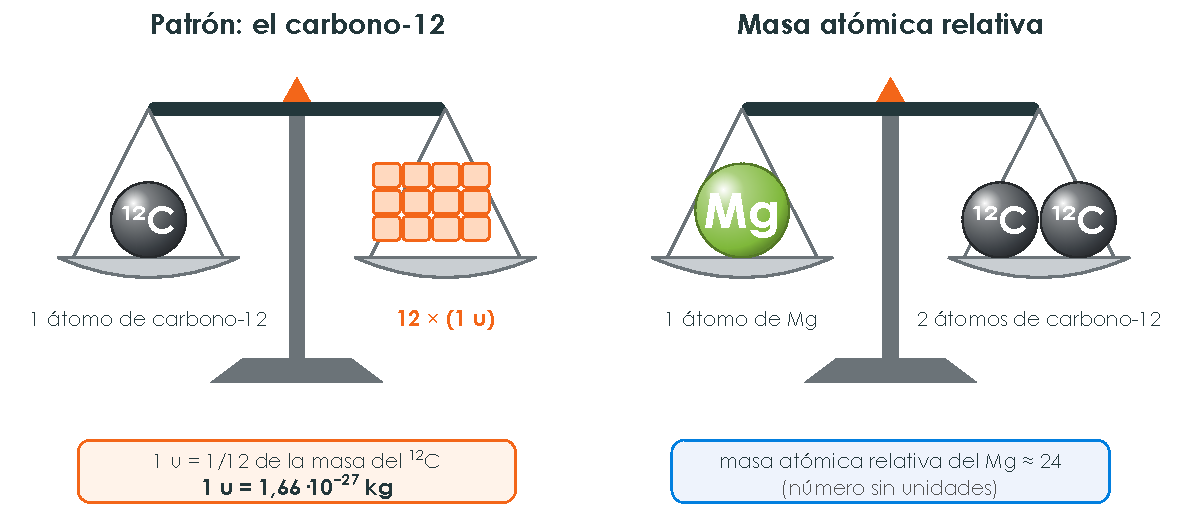
\includegraphics[width=0.75\linewidth]{FigurasSVG/UD0_Conocimientos_Basicos/pdf/UD0_01_unidad_masa_atomica.pdf}
    \caption{Unidad de masa atómica y masa atómica relativa}
    \label{fig:unidad-masa-atomica}
\end{figure}

\textbf{Masa atómica (promedio) de un elemento:} debido a la existencia de isótopos, se toma como masa atómica de un elemento a la masa promediada de sus isótopos.
\begin{centeredequation}
    M_{at}\ = \dfrac{\sum_{i=1}^{n} (\text{Abundancia relativa (en \%)} \times \text{masa atómica del isótopo})}{100}
\end{centeredequation}

\textbf{Masa molecular:} Se obtiene sumando la masa de los átomos que forman la molécula.

En los elementos que forman moléculas, no se debe confundir la masa atómica con la molecular.

En los compuestos iónicos no hay moléculas, sino iones, por lo cual algunos autores utilizan el término masa fórmula en vez de masa molecular, que se define como la masa de una fórmula de sólido iónico, y se calcula igual que la masa molecular.

\textbf{Mol:} cantidad de sustancia que contiene tantas partículas (átomos, moléculas, iones) como átomos hay en 12 gramos de Carbono-12.
Este número se llama \textbf{Número de Avogadro} \( N_A = \num{6.022e23} \).

\textbf{Mol de átomos de un elemento}, es la cantidad de dicho elemento que contiene el \( N_A \) de átomos.
\textbf{Mol de moléculas de un elemento o compuesto}, es la cantidad de dicho elemento o compuesto que contiene el \( N_A \) de moléculas.

\textbf{Masa molar:} es la masa de un mol de una sustancia.
\begin{itemize}
    \item Si es de 1 mol de átomos, también se llama átomo-gramo: es la masa del NA de átomos de dicho elemento, y es igual a la masa atómica expresada en gramos.
    \item Si es de 1 mol de moléculas, también se llama molécula-gramo: es la masa del NA de moléculas de dicho elemento o compuesto, y es igual a la masa molecular expresada en gramos.
\end{itemize}


\begin{itemize}
    \item M\textsubscript{atómica} H = \qty{1}{\uma} \( \Rightarrow \) masa de 1 mol de átomos (1 átomo-g) de H = \qty{1}{\g}, y contiene \num{6.022e23} átomos de H.
    \item M\textsubscript{molec} H2 = 2 u. Masa de 1 mol de moléculas (1 molécula-g) de H2 = 2 g, y contiene el NA de moléculas de H2.
    \item M\textsubscript{molec} H2O = 18 u. Masa de 1 mol de moléculas (1 molécula-g) de agua = 18 g, y contiene el NA de moléculas de H2O.
    \item Para hallar el número de moles de átomos o moles de moléculas:
    \begin{centeredequation}
        n = \dfrac{m(g)}{\text{M}_{\text{atómica}}\;\left( \unit{\g\per\mol}\right)}
    \end{centeredequation}
    También se puede hacer utilizando factores de conversión (se recomienda)
    Si partimos de \qty{10}{\g} de \ch{H20} el cálculo de los moles utilizando factores de conversión y sabiendo que la masa molar del \ch{H2O} es \qty{18}{\g\per\mol}:
    \begin{centeredequation}
        18 \cancelred{\unit{\g}} \cdot \dfrac{1\ \unit{\mol}}{18 \cancelred{\unit{\g}}} = \qty{1}{\mol}
    \end{centeredequation}
\end{itemize}


\begin{figure}[H]
    \centering
    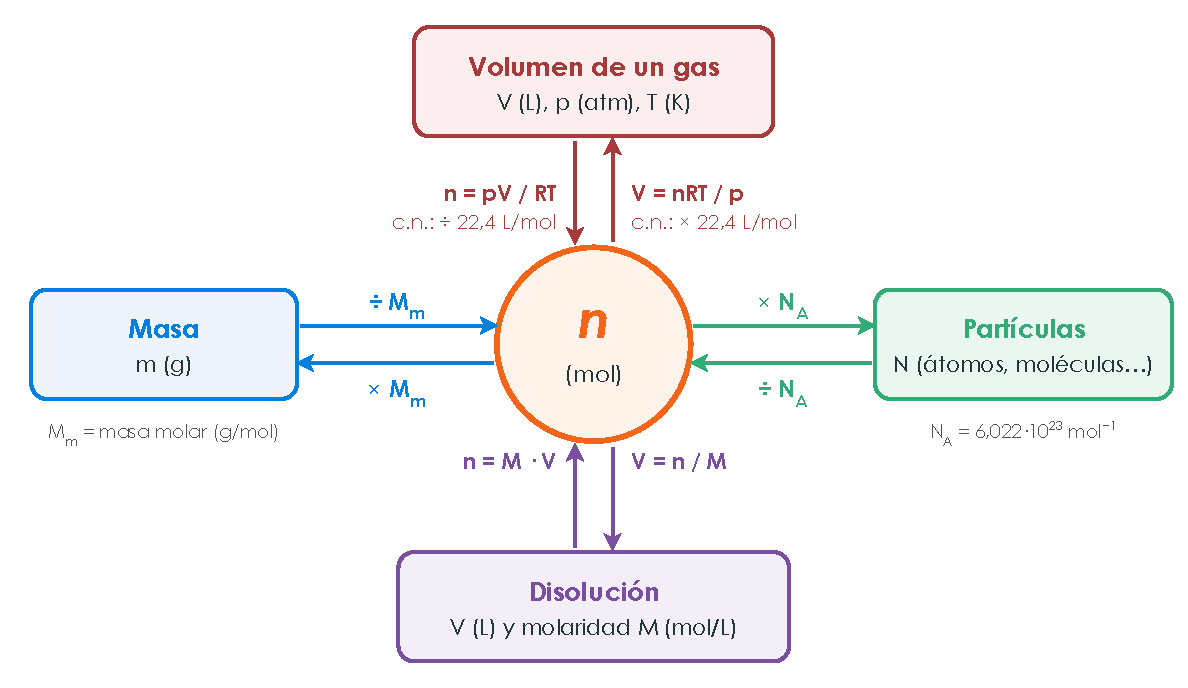
\includegraphics[width=0.8\linewidth]{FigurasSVG/UD0_Conocimientos_Basicos/pdf/UD0_02_mol_magnitud_central.pdf}
    \caption{El mol como magnitud central de los cálculos químicos}
    \label{fig:mol-magnitud-central}
\end{figure}

\section{Disoluciones}
\begin{definition}[Disolución]
    es una mezcla homogénea de dos o más sustancias puras y de composición variable, es decir, su composición y propiedades son las mismas en todos los puntos y además la composición se puede modificar.
\end{definition}

En una disolución tiene lugar la dispersión, la difusión, de las partículas de una sustancia llamada soluto entre las partículas de otra sustancia llamada disolvente.
Para distinguir el soluto del disolvente, hay que tener presente que el disolvente siempre tiene el mismo estado físico que la disolución y si ambos componentes tienen el mismo estado físico que la disolución, se toma como disolvente el que esté en mayor cantidad. Dependiendo del estado físico de los componentes hay 9 tipos de disoluciones, las más importantes son las disoluciones sólido-líquido y dentro de estas, las disoluciones acuosas, en las que se toma el agua como disolvente, aunque esté en menor cantidad.

\begin{figure}[H]
    \centering
    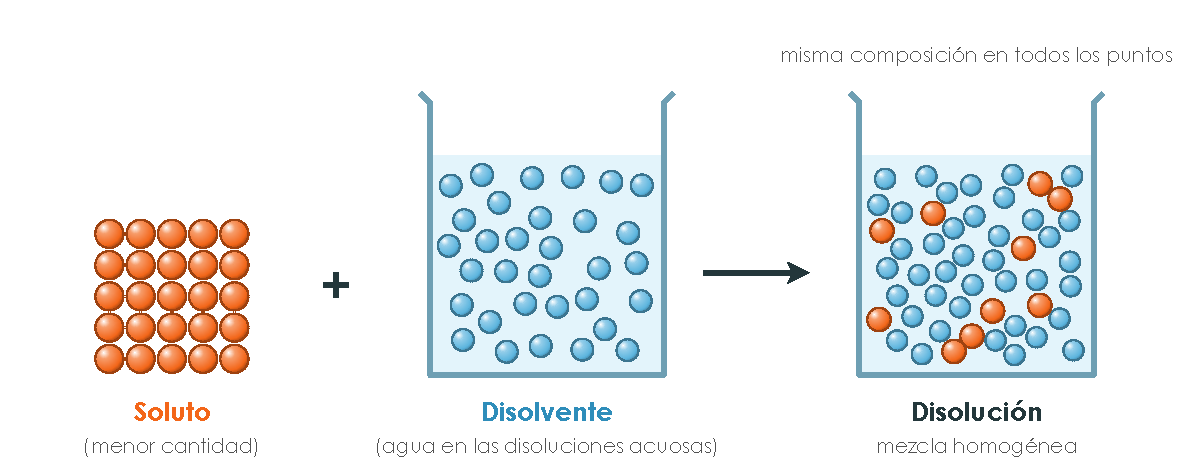
\includegraphics[width=0.8\linewidth]{FigurasSVG/UD0_Conocimientos_Basicos/pdf/UD0_03_disolucion_soluto_disolvente.pdf}
    \caption{El soluto se dispersa entre las partículas del disolvente}
    \label{fig:soluto-disolvente}
\end{figure}

\subsection{Concentración de una disolución}

\begin{definition}[Concentración]
    La \textbf{concentración} de una disolución indica la composición de la misma, es decir, la proporción entre el soluto y el disolvente.
\end{definition}
Se puede expresar de varias formas:
\begin{itemize}
    \item \textbf{\% en masa}: indica la masa de soluto que hay disuelta en 100 unidades de masa de disolución.
    \begin{centeredequation}
        \text{\% en masa} = \dfrac{\text{masa de soluto}}{\text{masa de disolución}} \times 100
    \end{centeredequation}
    \item \textbf{\% en volumen}: indica el volumen de soluto que hay disuelto en 100 unidades de volumen de disolución.
    \begin{centeredequation}
        \text{\% en volumen} = \dfrac{\text{volumen de soluto}}{\text{volumen de disolución}} \times 100
    \end{centeredequation}
    \item \textbf{g/L}: indica los gramos de soluto que hay disueltos en \qty{1}{\litre} de disolución.
    \begin{centeredequation}
        \text{g/L} = \dfrac{\text{m(g) de soluto}}{\text{V (L) de disolución}}
    \end{centeredequation}
    \begin{remark}
        Es importante no confundirlo con la densidad, en este caso el volumen es de la \textbf{disolución} mientras que la densidad nos dice la masa que hay por unidad de volumen de ese compuesto.
    \end{remark}
    \item \textbf{Molaridad (M)}: indica el número de moles disueltos en \qty{1}{\litre} de disolución.
    \begin{centeredequation}
        M = \dfrac{\text{n de soluto}}{\text{V (L) de disolución}}
    \end{centeredequation}
    Los moles (n) los podemos calcular:
    \begin{centeredequation}
        n = \dfrac{\text{m (g) de soluto}}{\text{M}_{\text{molar}} \left(\unit{g\per\mol} \right)}
    \end{centeredequation}
    \item \textbf{Normalidad (N)}: indica los equivalentes-gramo de soluto que hay disueltos en \qty{1}{\litre} de disolución.
    \begin{centeredequation}
        N = \dfrac{\text{nº de eq-g}}{\text{V (L) de disolución}}
    \end{centeredequation}
    El equivalente-gramo, representado como \textbf{eq-g}, es una unidad de medida química que representa la cantidad de una sustancia que reacciona con, o sustituye a, una cantidad estándar de otra sustancia química específica.
    \begin{centeredequation}
        \text{eq-g} = \dfrac{\text{m (g) de soluto}}{\text{P}_\text{eq}}
    \end{centeredequation}

    A diferencia del mol, que es una medida de sustancia basada puramente en el número de partículas, el equivalente-gramo depende de la \textbf{reactividad} de la sustancia y del tipo de reacción que tengamos. Siendo P\textsubscript{eq}:
    \begin{centeredequation}
        \text{P}_\text{eq} = \dfrac{\text{Masa molar}}{\text{valencia}}
    \end{centeredequation}
    La \textbf{valencia} es el número de \ch{H+} o \ch{OH-} transferidos en una reacción ácido-base o el número de electrones que ha perdido o ganado en una reacción redox.

    Podemos relacionar fácilmente la normalidad con la molaridad según la ecuación:
    \begin{centeredequation}
        N = M \cdot \text{valencia}
    \end{centeredequation}
    \item \textbf{Molalidad (m)}: indica los moles de soluto disueltos en \qty{1}{\kg} de disolvente.
    \begin{centeredequation}
        m = \dfrac{\text{n de soluto}}{\text{kg de disolvente}}
    \end{centeredequation}
    \item \textbf{Fracción molar del soluto (\( \chi_{s} \))}: indica los moles de soluto disueltos en \qty{1}{\mol} de disolución y se representa con el símbolo \( \chi_s \). Su valor siempre está entre 0 y 1.
    \begin{centeredequation}
        \chi_{s} = \dfrac{\text{moles de soluto}}{\text{moles de disolución}} = \dfrac{\text{moles de soluto}}{\text{moles de soluto} + \text{moles de disolvente}}
    \end{centeredequation}
    \item \textbf{Fracción molar del disolvente}: indica los moles de disolvente que tenemos en \qty{1}{\mol} de disolución y se representa con \( \chi_d \). Su valor también está entre 0 y 1.
    \begin{centeredequation}
        \chi_{d} = \dfrac{\text{moles de disolvente}}{\text{moles de disolución}} = \dfrac{\text{moles de disolvente}}{\text{moles de soluto} + \text{moles de disolvente}}
    \end{centeredequation}
    Se cumple también que:
    \begin{centeredequation}
        \chi_s + \chi_d = 1
    \end{centeredequation}
\end{itemize}


\section{Leyes de los gases}

\subsection{Ley de los gases ideales}

\begin{definition}[Gas ideal]
    es una sustancia simple compresible y pura de naturaleza especial y se considera un modelo \textbf{teórico} o \textbf{hipotético} en el que sus partículas se desplazan aleatoriamente y no \textbf{interactúan entre sí} y por tanto no existen fuerzas de atracción o repulsión.
\end{definition}

Las leyes de Boyle-Mariotte, Charles y Gay-Lussac se pueden combinar en una ecuación general denominada ecuación general de los gases ideales:

\begin{centeredequation}
    p\cdot V = n \cdot R \cdot T
\end{centeredequation}

\begin{figure}[H]
    \centering
    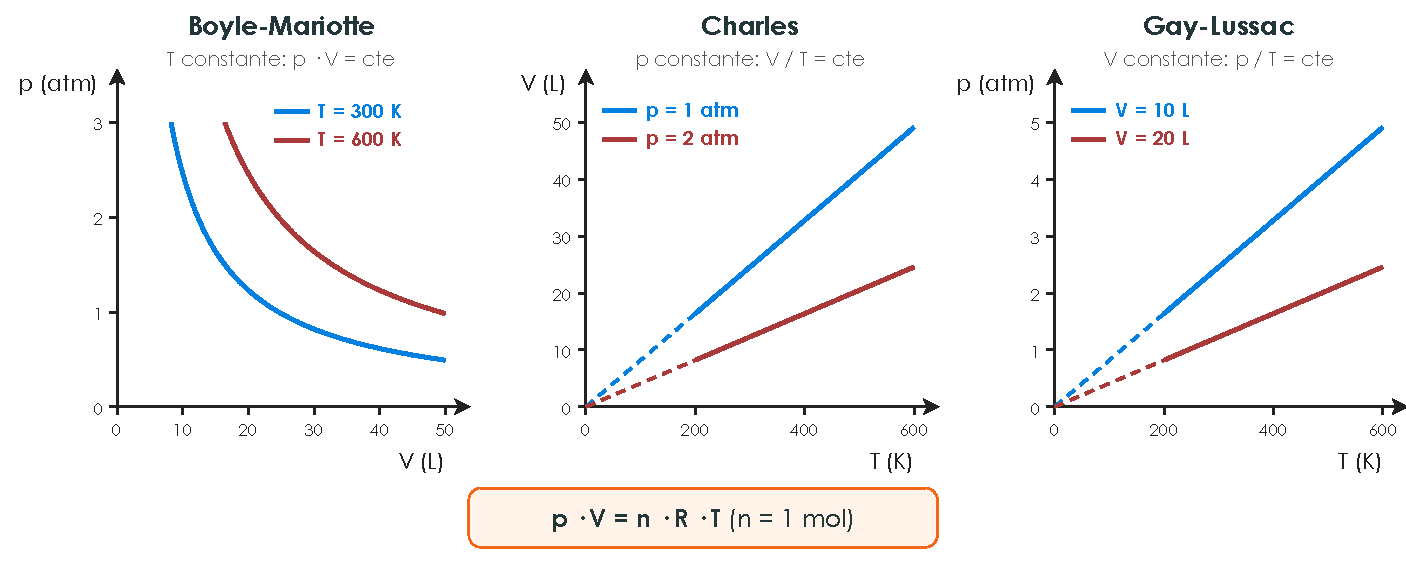
\includegraphics[width=1.0\linewidth]{FigurasSVG/UD0_Conocimientos_Basicos/pdf/UD0_04_leyes_gases.pdf}
    \caption{Leyes de Boyle-Mariotte, Charles y Gay-Lussac (calculadas para \qty{1}{\mol} de gas ideal)}
    \label{fig:leyes-gases}
\end{figure}

Si tomamos el valor \( R = \ctegases \), debemos tener la presión en atmósferas, la temperatura en Kelvin y el volumen en litros.

\begin{definition}[volumen molar]
    es el volumen ocupado por un mol de un gas ideal que será siempre el mismo en las mismas condiciones de presión y temperatura.
\end{definition}

Llamamos condiciones normales (cn) cuando la presión \( p = \qty{1}{\atmosphere} \) y la temperatura \( T = \qty{0}{\celsius} \longrightarrow T = \qty{273}{\kelvin}\). El volumen ocupado por cualquier gas ideal en estas condiciones siempre es de \( V_{{cn}} = \qty{22.4}{\litre} \). En la última actualización, la IUPAC acepta establecer este volumen molar en condiciones normales como \(V_{cn} = \qty{22.7}{\litre} \). Este cambio se debe a que la IUPAC ha modificado la presión de referencia para las condiciones normales, que ha pasado de \( \qty{1}{\atmosphere} = \qty{101325}{\pascal} \) a \( \qty{1}{\bar} = \qty{e5}{\pascal} \).

\subsection{Ley de Dalton}

\begin{ley}[Ley de Dalton]
    La ley de Dalton o también llamada ley de las presiones parciales dice que: en una mezcla de gases, la presión total es la suma de las presiones parciales que ejerce cada gas de manera individual.
    \begin{centeredequation}
        p_T = \sum_{i=m}^{n} p_i \longrightarrow p_T = p_{m} + p_{m+1} + p_{m+2} + ... + p_{n}
    \end{centeredequation}
\end{ley}

Si tenemos una mezcla de \( \ch{CO2} + \ch{CO} + \ch{H2} \) en un recipiente cerrado, la presión total de la mezcla será la suma de las presiones de cada compuesto, quedando que:
\begin{centeredequation*}
    p_T = p_{\ch{CO2}} + p_{\ch{CO}} + p_{\ch{H2}}
\end{centeredequation*}

De esta ley se deduce que la presión de un determinado componente de la mezcla será igual al producto de la fracción molar de ese componente por la presión total. Si consideramos el compuesto \( i \) en una mezcla tendremos que:
\begin{centeredequation}
    p_i = \chi_i \cdot p_T
\end{centeredequation}


\begin{figure}[H]
    \centering
    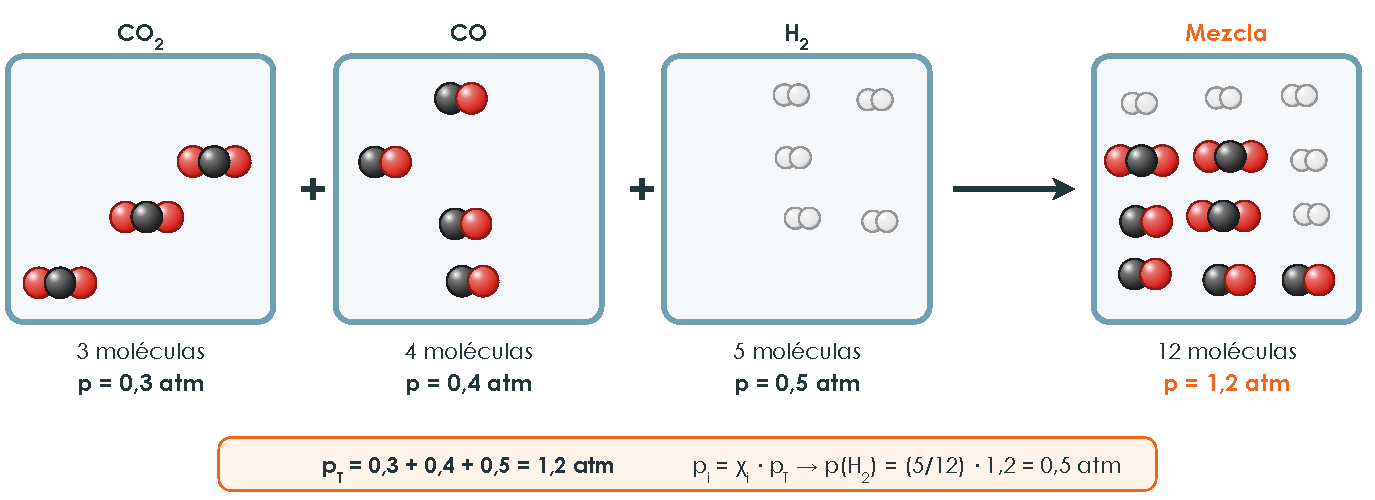
\includegraphics[width=1.0\linewidth]{FigurasSVG/UD0_Conocimientos_Basicos/pdf/UD0_05_ley_dalton.pdf}
    \caption{Ley de Dalton: la presión total es la suma de las presiones parciales}
    \label{fig:ley-dalton}
\end{figure}

\section{Fórmulas}

En los compuestos iónicos, la fórmula indica la proporción en la que se encuentran los iones en el cristal, mientras que para los compuestos covalentes se pueden utilizar varios tipos de fórmulas:
\begin{itemize}
    \item \negsubro{Fórmula empírica:} indica la mínima relación entre átomos de una molécula.
    \item \negsubro{Fórmula molecular:} indica el número real de átomos que forman la molécula.
    \item \negsubro{Fórmula estructural:} indica como están enlazados los átomos en la molécula.
\end{itemize}

En los compuestos inorgánicos (excepto los peróxidos), las fórmulas empírica y molecular coinciden, pero no es así en los compuestos orgánicos.

\begin{example}
    Para el agua tendremos que:
    \begin{itemize}
        \item La fórmula empírica es \ch{H2O}.
        \item La fórmula molecular es \ch{H2O}.
    \end{itemize}
    Para el peróxido de hidrógeno tendremos que:
    \begin{itemize}
        \item La fórmula empírica es \ch{HO}.
        \item La fórmula molecular es \ch{H2O2}.
    \end{itemize}
    Para el etano tendremos que:
    \begin{itemize}
        \item La fórmula empírica es \ch{CH3}.
        \item La fórmula molecular es \ch{C2H6}.
    \end{itemize}

\end{example}


\begin{figure}[H]
    \centering
    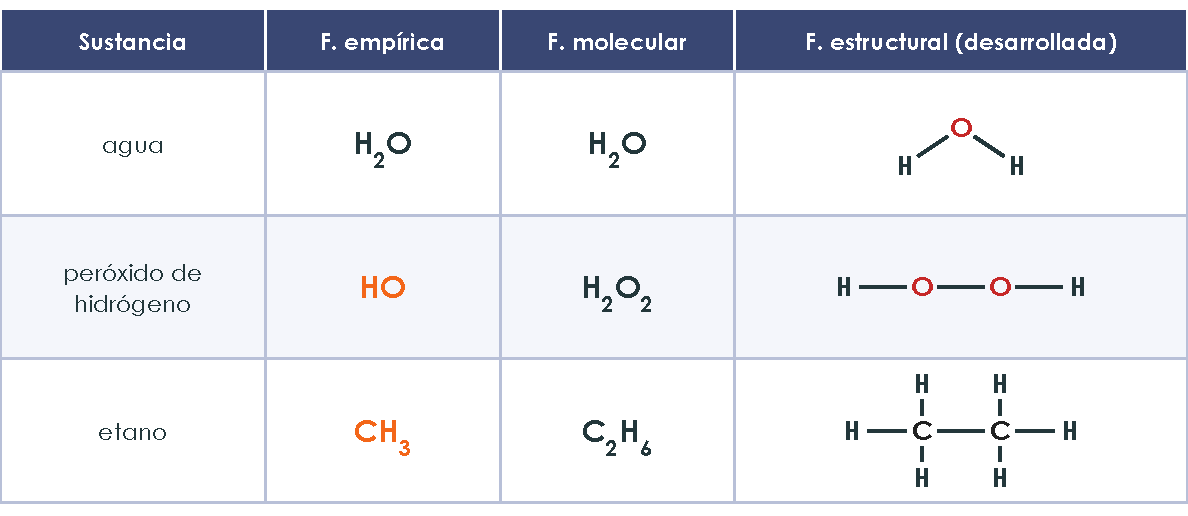
\includegraphics[width=0.8\linewidth]{FigurasSVG/UD0_Conocimientos_Basicos/pdf/UD0_06_tipos_formulas.pdf}
    \caption{Fórmulas empírica, molecular y estructural}
    \label{fig:tipos-formulas}
\end{figure}

\section{Reacciones químicas}

Una reacción química es el proceso mediante el cual, a partir de unas sustancias llamadas reactivos, se obtienen otras sustancias distintas llamadas productos.
Las reacciones se representan mediante las llamadas ecuaciones químicas, en las que aparecen las fórmulas de los reactivos y de los productos separados por una flecha, que indica el sentido en el que tiene lugar la reacción. Ahora bien, en una reacción la masa se conserva (ley de conservación de la masa de Lavoisier), ya que tan solo tiene lugar el reagrupamiento de los átomos: el número de átomos de cada elemento es el mismo antes y después de la reacción. Para que la ecuación química esté ajustada, se introducen unos coeficientes que indican el número de moléculas (y por tanto, también de moles) de cada sustancia que interviene en la reacción.

\begin{centeredequation}
    \ch{N2 + 3 H2 -> 2 NH3}
\end{centeredequation}


En este ejemplo, podemos ver como 1 molécula de \ch{N2} reacciona con 3 moléculas de \ch{H2} para formar 2 moléculas de \ch{NH3}. Podemos decir también que 1 mol de \ch{N2} reacciona con 3 moles de \ch{H2} para formar 2 moles de \ch{NH3}.

\begin{figure}[H]
    \centering
    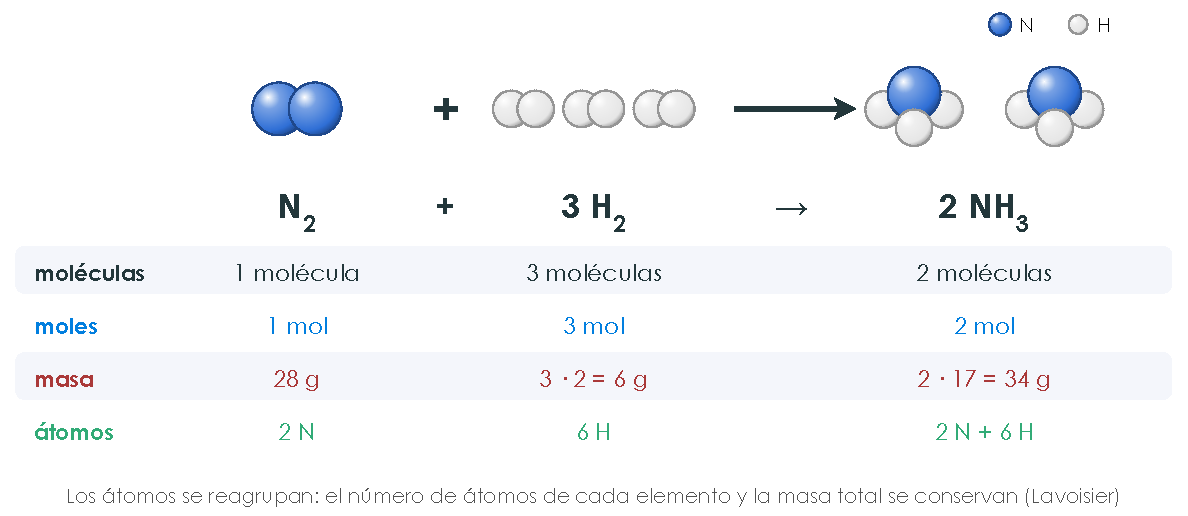
\includegraphics[width=0.8\linewidth]{FigurasSVG/UD0_Conocimientos_Basicos/pdf/UD0_07_reaccion_N2_H2.pdf}
    \caption{Interpretación de la ecuación química \ch{N2 + 3 H2 -> 2 NH3}}
    \label{fig:reaccion-N2-H2}
\end{figure}

\subsection{Cálculos estequiométricos}

La estequiometría es el estudio cuantitativo de las reacciones. Conocida la cantidad de una sustancia, se puede calcular la cantidad de otra sustancia que intervenga en la reacción, valiéndonos de los coeficientes estequiométricos, ya que éstos indican la relación en moles, y en el caso de que todas las sustancias sean gaseosas también indican la relación en volumen (litros, \unit{\cubic\centi\metre}, etc.), lo cual se deduce de la hipótesis de Avogadro.

Con la estequiometría, podemos:
\begin{itemize}
    \item Determinar las cantidades de reactivos y productos mediante relaciones mol-mol, masa-masa, masa-volumen y volumen-volumen.
    \item En muchas reacciones, las cantidades de los reactivos no están en las proporciones exactas de reacción; en tal caso, las cantidades obtenidas de los productos están determinadas por el reactivo limitante, esto es, el reactivo que se consume antes.
    \item En la práctica, la mayoría de las veces no se obtiene la cantidad de producto que se deduce de la estequiometría de la reacción, debido a que no llegan a consumirse totalmente los reactivos y que además de la reacción principal se producen otras reacciones secundarias, lo que hace que el rendimiento de la reacción no sea del 100\%.
    \begin{centeredequation}
        \text{\% de rendimiento} = \dfrac{\text{cantidad del producto obtenido experimentalmente}}{\text{cantidad del producto que se debe obtener de forma teórica}} \times 100
    \end{centeredequation}
    Por ejemplo, un rendimiento del 80\% significa que de cada \qty{100}{\mol} que teóricamente deberían obtenerse, en la práctica tan solo se han obtenido \qty{80}{\mol}.
    \begin{remark}
        Para evitar errores en los cálculos estequiométricos se aconseja siempre pasar todo y trabajar en los cálculos con moles y luego calcular los gramos de cada sustancia según se pida.
    \end{remark}
    \item A veces, el reactivo no es puro o se encuentra en disolución como soluto; en tal caso, hay que determinar la cantidad de reactivo que realmente interviene en la reacción. Si un compuesto tiene una pureza del 70\% (si no se especifica, supondremos que el porcentaje será en masa), quiere decir que de \qty{100}{\g} de ese compuesto, tan solo \qty{70}{\g} son puros.
\end{itemize}

\begin{figure}[H]
    \centering
    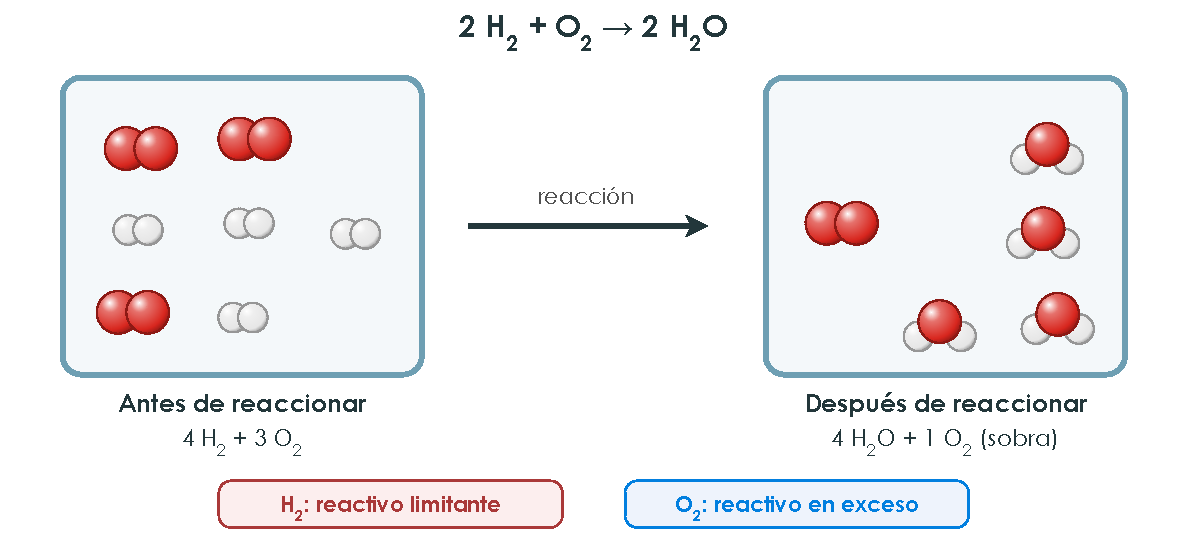
\includegraphics[width=0.75\linewidth]{FigurasSVG/UD0_Conocimientos_Basicos/pdf/UD0_08_reactivo_limitante.pdf}
    \caption{Reactivo limitante y reactivo en exceso}
    \label{fig:reactivo-limitante}
\end{figure}

\begin{figure}[H]
    \centering
    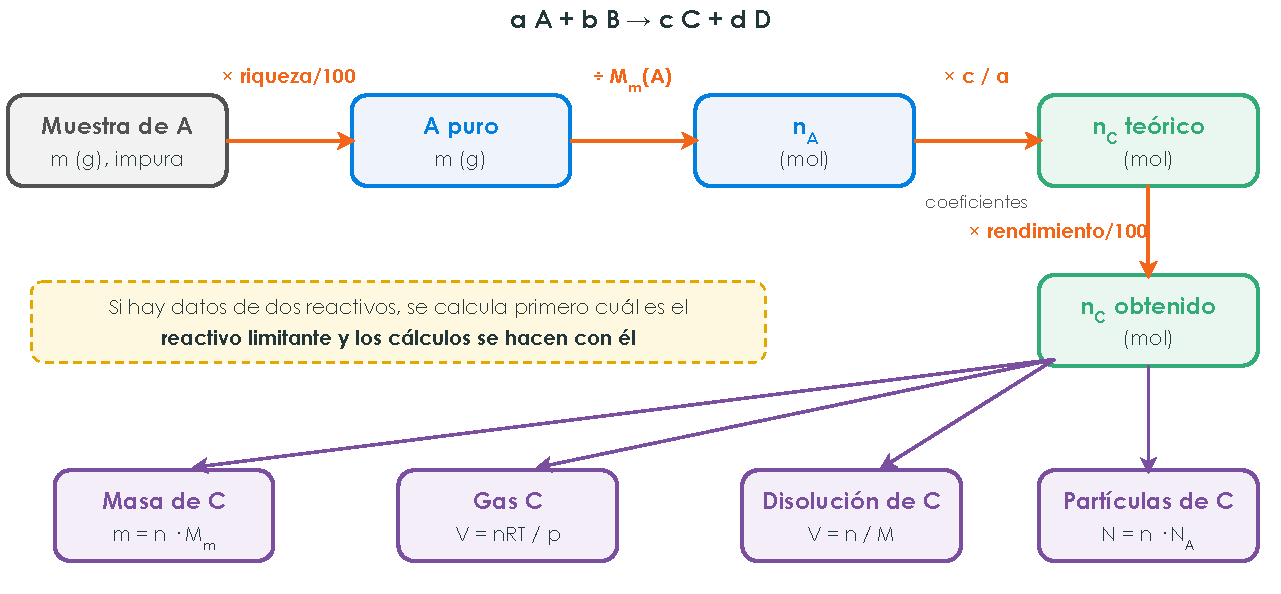
\includegraphics[width=0.9\linewidth]{FigurasSVG/UD0_Conocimientos_Basicos/pdf/UD0_09_ruta_estequiometrica.pdf}
    \caption{Pasos de un cálculo estequiométrico}
    \label{fig:ruta-estequiometrica}
\end{figure}


    \newpage

    
\section{Ejercicios}

\subsection{Ejercicios sobre disoluciones}

\begin{exercise}
    En 35 g de agua se disuelven 5 g de ácido clorhídrico. La densidad de la disolución resultante es \qty{1.06}{\g\per\cubic\centi\metre}. Halla la concentración de la disolución: a) en \% en masa , b) en \unit{\g\per\litre} , c) molaridad y d) normalidad.
    Sol: a) 12,5 \%,  b) \qty{132.5}{\g\per\litre},  c) \qty{3.63}{\M},  d) \qty{3.63}{\N}.

    \begin{solu}
        1. \textbf{Masa total:} $m_{dis} = 5\,\text{g (soluto)} + 35\,\text{g (disolvente)} = 40\,\text{g}$.

        a) \textbf{\% en masa:}
        \[ \% = \dfrac{\qty{5}{\g}}{\qty{40}{\g}} \cdot 100 = \mathbf{\textcolor{blue}{12,5 \%}} \]

        b) \textbf{Concentración en \unit{\g\per\litre}:}
        \[ C = \dfrac{\qty{5}{\g} \text{ sol.}}{\qty{40}{\g} \text{ dis.}} \cdot \dfrac{\qty{1.06}{\g} \text{ dis.}}{\qty{1}{\mL}} \cdot \dfrac{\qty{1000}{\mL}}{\qty{1}{\L}} = \mathbf{\textcolor{blue}{\qty{132.5}{\g\per\L}}} \]

        c) \textbf{Molaridad (M):} ($M_m HCl = \qty{36.5}{\g\per\mol}$)
        \[ M = \dfrac{\qty{132.5}{\g}}{\qty{1}{\L}} \cdot \dfrac{\qty{1}{\mol}}{\qty{36.5}{\g}} = \mathbf{\textcolor{blue}{\qty{3.63}{\M}}} \]

        d) \textbf{Normalidad (N):} Al ser $HCl$ monoprótico (un solo hidrógeno) ($v=1$), $N = M$. \textbf{\textcolor{blue}{\qty{3.63}{\N}}}.
    \end{solu}

\end{exercise}

\begin{exercise}
    Un ácido nítrico concentrado, de densidad \qty{1.405}{\g\per\cubic\centi\metre}, contiene 68,1 \% en masa de \ch{HNO3}. Calcula la molaridad, normalidad y molalidad de este ácido.
    Sol: \qty{15.18}{\M},  \qty{15.18}{\N} y  \qty{33.96}{\molal}.
    \begin{solu}
        Usamos factores de conversión sobre una base de \qty{1}{\L} de disolución:
        \[ M = \dfrac{\qty{1.405}{\g} \text{ dis.}}{\qty{1}{\mL} \text{ dis.}} \cdot \dfrac{\qty{1000}{\mL}}{\qty{1}{\L}} \cdot \dfrac{\qty{68.1}{\g} \text{ puro}}{\qty{100}{\g} \text{ dis.}} \cdot \dfrac{\qty{1}{\mol}}{\qty{63}{\g}} = \mathbf{\textcolor{blue}{\qty{15.18}{\M}}} \]
        $N = M \cdot 1 = \mathbf{\textcolor{blue}{\qty{15.18}{\N}}}$.

        Para la \textbf{molalidad}, en \qty{100}{\g} de disolución hay \qty{68.1}{\g} de soluto y \qty{31.9}{\g} de agua:
        \[ m = \dfrac{\qty{68.1}{\g} \text{ sol.}}{\qty{31.9}{\g} \text{ agua}} \cdot \dfrac{\qty{1000}{\g}}{\qty{1}{\kg}} \cdot \dfrac{\qty{1}{\mol}}{\qty{63}{\g}} = \mathbf{\textcolor{blue}{\qty{33.96}{\molal}}} \]
    \end{solu}

\end{exercise}

\begin{exercise}
    Calcula la fracción molar del metanol (\ch{CH3OH}) en una disolución acuosa \qty{0.1}{\M}. Sol: 1,79 . 10 3.
    \begin{solu}
        En una disolución acuosa diluida, el volumen de la disolución es aproximadamente el del agua ($\rho_{agua} \approx \qty{1}{\kg\per\L}$). En \qty{1}{\L} (\qty{1000}{\g}) de agua hay:
        \[ n_{agua} = \dfrac{\qty{1000}{\g}}{\qty{18}{\g\per\mol}} = \qty{55.55}{\mol} \]
        Moles de metanol = \qty{0.1}{\mol} (por definición de \qty{0.1}{\M}).
        \[ \chi_{metanol} = \dfrac{n_{sol}}{n_{sol} + n_{dis}} = \dfrac{0,1}{0,1 + 55,55} = \mathbf{\textcolor{blue}{1,79 \cdot 10^{-3}}} \]
    \end{solu}
\end{exercise}

\begin{exercise}
    Si \qty{9}{\L} de cloruro de hidrógeno, medidos a \qty{20}{\celsius} y \qty{750}{\mmhg}, se disuelven en el agua necesaria para dar \qty{290}{\mL} disolución, ¿cuál es la M de la disolución?.
    Sol: \qty{1.27}{\M}.

    \begin{solu}
        1. \textbf{Cálculo de moles de soluto (Gas):} Usamos $PV = nRT$.
        $P = \dfrac{750}{760} \unit{\atm} = \qty{0.987}{\atm}$; $V = \qty{9}{\L}$; $T = 20 + 273 = \qty{293}{\K}$.
        \[ n = \dfrac{P \cdot V}{R \cdot T} = \dfrac{\qty{0.987}{\atm} \cdot \qty{9}{\L}}{\qty{0.082}{\atm\L\per\mol\per\K} \cdot \qty{293}{\K}} = \qty{0.3694}{\mol} \]

        2. \textbf{Molaridad:} $V_{dis} = \qty{0.290}{\L}$.
        \[ M = \dfrac{\qty{0.3694}{\mol}}{\qty{0.290}{\L}} = \mathbf{\textcolor{blue}{\qty{1.27}{\M}}} \]
    \end{solu}
\end{exercise}

\begin{exercise}
    ¿Qué volumen de ácido nítrico con el 68\% de riqueza y \qty{1.4}{\g\per\cubic\centi\metre} de densidad se necesita para preparar \qty{3}{\L} de una disolución \qty{0.5}{\M} de ácido nítrico?.
    Sol: \qty{99.26}{\cc}

    \begin{solu}
        1. \textbf{Moles necesarios:} $n = \qty{3}{\L} \cdot \qty{0.5}{\mol\per\L} = \qty{1.5}{\mol}$.

        2. \textbf{Cálculo del volumen del ácido comercial:}
        \[ V = \qty{1.5}{\mol} \cdot \dfrac{\qty{63}{\g}}{\qty{1}{\mol}} \cdot \dfrac{\qty{100}{\g} \text{ dis.}}{\qty{68}{\g} \text{ puro}} \cdot \dfrac{\qty{1}{\mL} \text{ dis.}}{\qty{1.4}{\g} \text{ dis.}} = \mathbf{\textcolor{blue}{\qty{99.26}{\mL}}} \]
    \end{solu}
\end{exercise}

\begin{exercise}
    Disponemos de \qty{90}{\g} de cloruro de magnesio y queremos disolverlo en agua hasta obtener una disolución de concentración \qty{1.2}{\M}. ¿Qué volumen de disolución prepararemos?.
    Sol: \qty{0.787}{\L}.

    \begin{solu}
        1. \textbf{Moles de soluto ($MgCl_2$):} $M_m \approx 24.3 + 2(35.5) = \qty{95.3}{\g\per\mol}$.
        \[ n = \dfrac{\qty{90}{\g}}{\qty{95.3}{\g\per\mol}} = \qty{0.944}{\mol} \]

        2. \textbf{Volumen necesario:}
        \[ V = \dfrac{n}{M} = \dfrac{\qty{0.944}{\mol}}{\qty{1.2}{\mol\per\L}} = \mathbf{\textcolor{blue}{\qty{0.787}{\L}}} \]
    \end{solu}
\end{exercise}

\begin{exercise}
    Calcula la molaridad, normalidad, molalidad y fracción molar del soluto de una disolución de ácido sulfúrico de densidad \qty{1.198}{\g\per\cc} que contiene 27 \% de ácido sulfúrico en peso.
    Sol: \qty{3.3}{\M}, \qty{6.6}{\N},  \qty{3.78}{\molal} y 0,064.

    \begin{solu}
        Base: \qty{1}{\L} de disolución. $M_m \ch{H2SO4} = \qty{98}{\g\per\mol}$.

        a) \textbf{Molaridad:}
        \[ M = \dfrac{\qty{1198}{\g} \text{ dis.}}{\qty{1}{\L}} \cdot \dfrac{\qty{27}{\g} \text{ puro}}{\qty{100}{\g} \text{ dis.}} \cdot \dfrac{\qty{1}{\mol}}{\qty{98}{\g}} = \mathbf{\textcolor{blue}{\qty{3.3}{\M}}} \]

        b) \textbf{Normalidad:} Como tiene 2 hidrógenos: $N = 3.3 \cdot 2 = \mathbf{\textcolor{blue}{\qty{6.6}{\N}}}$.

        c) \textbf{Molalidad:} Masa agua en \qty{100}{\g} dis. = $100 - 27 = \qty{73}{\g}$.
        \[ m = \dfrac{\qty{27}{\g} \text{ sol.}}{\qty{73}{\g} \text{ agua}} \cdot \dfrac{\qty{1000}{\g}}{\qty{1}{\kg}} \cdot \dfrac{\qty{1}{\mol}}{\qty{98}{\g}} = \mathbf{\textcolor{blue}{\qty{3.78}{\molal}}} \]

        d) \textbf{Fracción molar ($\chi$):} $n_{sol} = \dfrac{27}{98} = \qty{0.2755}{\mol}$; $n_{agua} = \dfrac{73}{18} = \qty{4.055}{\mol}$.
        \[ \chi = \dfrac{0.2755}{0.2755 + 4.055} = \mathbf{\textcolor{blue}{0,064}} \]
    \end{solu}
\end{exercise}

\begin{exercise}
    ¿Cuál será la molaridad de una disolución de ácido nítrico preparada por dilución a \qty{500}{\mL}, de \qty{32}{\mL} de un ácido concentrado de densidad \qty{1.42}{\gpcc} y una riqueza de ácido nítrico de 69,5 \%?.
    Sol: \qty{1}{\M}.
    \begin{figure}[H]
        \centering
        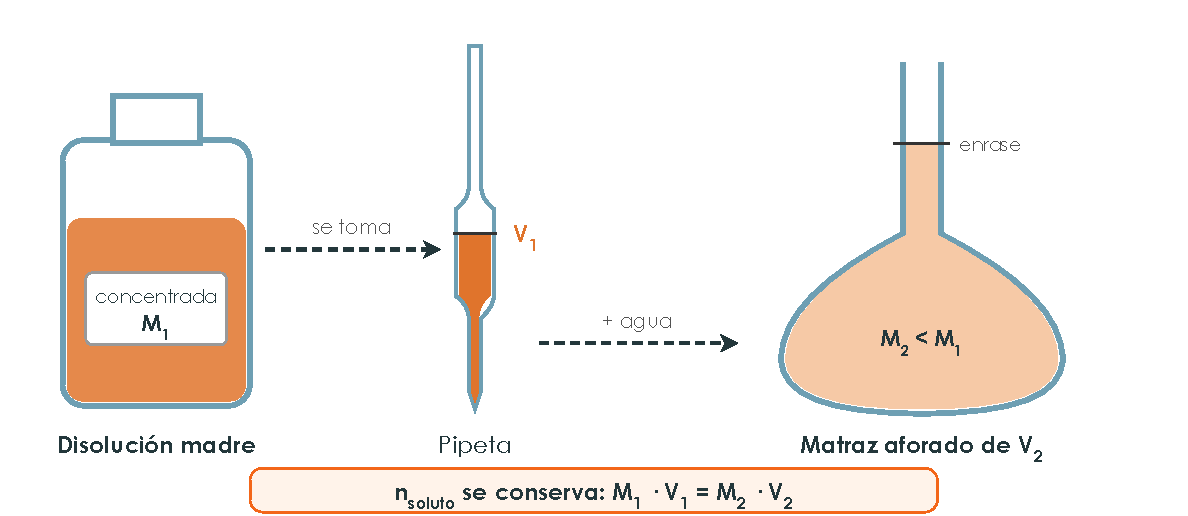
\includegraphics[width=0.75\linewidth]{FigurasSVG/UD0_Conocimientos_Basicos/pdf/UD0_E01_dilucion.pdf}
        \caption{Preparación de una disolución por dilución}
        \label{fig:dilucion}
    \end{figure}

    \begin{solu}
        1. \textbf{Moles en la porción de \qty{32}{\mL}:}
        \[ n = \qty{32}{\mL} \cdot \dfrac{\qty{1.42}{\g}}{\qty{1}{\mL}} \cdot \dfrac{69.5}{100} \cdot \dfrac{\qty{1}{\mol}}{\qty{63}{\g}} = \qty{0.501}{\mol} \]

        2. \textbf{Molaridad final:} Al diluir a \qty{500}{\mL} (\qty{0.5}{\L}):
        \[ M = \dfrac{\qty{0.501}{\mol}}{\qty{0.5}{\L}} = \mathbf{\textcolor{blue}{\qty{1}{\M}}} \]
    \end{solu}
\end{exercise}

\begin{exercise}
    Un litro de ácido clorhídrico del 35\% en masa y densidad \qty{1.18}{\gpcc}, debe diluirse de tal manera que se obtenga ácido al 20 \%. ¿ Qué cantidad de agua deberá añadirse?.
    Sol: \qty{885}{\mL}.

    \begin{solu}
        1. \textbf{Masa inicial de la disolución:} $m_1 = \qty{1000}{\mL} \cdot \qty{1.18}{\g\per\mL} = \qty{1180}{\g}$.

        2. \textbf{Masa de soluto (HCl):} $m_{sol} = \qty{1180}{\g} \cdot 0.35 = \qty{413}{\g}$.

        3. \textbf{Masa de la disolución final (20\%):} El soluto no cambia.
        \[ m_2 = \dfrac{\qty{413}{\g}}{0.20} = \qty{2065}{\g} \]

        4. \textbf{Agua añadida:} $m_{agua} = 2065 - 1180 = \mathbf{\textcolor{blue}{\qty{885}{\g}}} \rightarrow \mathbf{\textcolor{blue}{\qty{885}{\mL}}}$.
    \end{solu}
\end{exercise}

\begin{exercise}
    Calcula la M de una disolución preparada mezclando \qty{50}{\mL} de ácido sulfúrico \qty{0.136}{\M} con \qty{90}{\mL} de una disolución de ácido sulfúrico \qty{0.068}{\M}.
    Sol: \qty{0.092}{\M}.
    \begin{solu}
        1. \textbf{Moles totales:}
        $n_1 = \qty{0.050}{\L} \cdot \qty{0.136}{\mol\per\L} = \qty{0.0068}{\mol}$ \\
        $n_2 = \qty{0.090}{\L} \cdot \qty{0.068}{\mol\per\L} = \qty{0.00612}{\mol}$ \\
        $n_{tot} = \qty{0.01292}{\mol}$
        2. \textbf{Volumen total:} $V_{tot} = 50 + 90 = \qty{140}{\mL} = \qty{0.140}{\L}$.
        3. \textbf{Molaridad:}
        \[ M = \dfrac{\qty{0.01292}{\mol}}{\qty{0.140}{\L}} = \mathbf{\textcolor{blue}{\qty{0.092}{\M}}} \]
    \end{solu}
\end{exercise}

\begin{exercise}
    Una disolución de ácido acético al 10\% tiene \qty{1.055}{\gpcc} de densidad, se desea saber:
    a) ¿cuál es su molalidad?. b) si añadimos un litro de agua a \qty{500}{\cc} de la disolución anterior, ¿cuál es el \% en peso y la normalidad de la nueva disolución? Sol: \qty{1.55}{\molal} , 3,45 \%, \qty{0.58}{\N}
    \begin{solu}
        a) \textbf{Molalidad:} $M_m \approx \qty{60}{\g\per\mol}$. En \qty{100}{\g} dis.: \qty{10}{\g} sol. y \qty{90}{\g} agua.
        \[ m = \dfrac{\qty{10}{\g} \text{ sol.}}{\qty{90}{\g} \text{ agua}} \cdot \dfrac{\qty{1000}{\g}}{\qty{1}{\kg}} \cdot \dfrac{\qty{1}{\mol}}{\qty{60}{\g}} = \mathbf{\textcolor{blue}{\qty{1.85}{\molal}}} \]

        b) \textbf{Dilución:} En \qty{500}{\mL} (\qty{0.5}{\L}) iniciales: \\
        Masa dis. = $500 \cdot 1.055 = \qty{527.5}{\g}$. \\
        Masa soluto = $527.5 \cdot 0.10 = \qty{52.75}{\g}$. \\
        Añadimos \qty{1}{\L} (\qty{1000}{\g}) de agua: \\
        Masa final dis. = $527.5 + 1000 = \qty{1527.5}{\g}$. \\
        $\% \text{ peso} = \dfrac{52,75}{1527,5} \cdot 100 = \mathbf{\textcolor{blue}{3,45 \%}}$. \\
        Normalidad (suponiendo volúmenes aditivos $V \approx \qty{1.5}{\L}$): \\
        $n = 52.75 / 60 = \qty{0.879}{\mol}$. $M = 0.879 / 1.5 = \qty{0.58}{\M}$. Como es monoprótico, \textbf{\textcolor{blue}{\qty{0.58}{\N}}}.
    \end{solu}
\end{exercise}

\subsection{Ejercicios sobre gases}

\begin{exercise}
    Un neumático de una motocicleta tiene un volumen de 10 litros y se llena de aire a una presión de 3 atm, a 27ºC. Después de circular varias horas, la T se eleva a 57ºC y el volumen se supone invariable. Calcula: a) la presión que habrá en el neumático, b) el volumen del gas si la presión hubiera aumentado sin variar la T.
    Sol: a) \qty{3.3}{\atm}, b) \qty{9.09}{\L}.

    \begin{solu}
        Datos: $V_1 = \qty{10}{\L}$, $P_1 = \qty{3}{\atm}$, $T_1 = 27 + 273 = \qty{300}{\K}$. \\
        a) Presión a $T_2 = 57 + 273 = \qty{330}{\K}$ ($V$ cte):
        \[ P_2 = P_1 \cdot \dfrac{T_2}{T_1} = \qty{3}{\atm} \cdot \dfrac{\qty{330}{\K}}{\qty{300}{\K}} = \mathbf{\textcolor{blue}{\qty{3,3}{\atm}}} \]
        b) Volumen si $P_2 = \qty{3,3}{\atm}$ a $T_1$ cte:
        \[ V_2 = \dfrac{P_1 \cdot V_1}{P_2} = \dfrac{\qty{3}{\atm} \cdot \qty{10}{\L}}{\qty{3,3}{\atm}} = \mathbf{\textcolor{blue}{\qty{9,09}{\L}}} \]
    \end{solu}
\end{exercise}

\begin{exercise}
    Un volumen de \qty{2.38}{\litre} de un gas, medido a \qty{97}{\celsius} y \qty{720}{\mmhg}, tiene una masa de \qty{2.81}{\g}. Calcula la masa molecular de dicho gas.
    Sol: 37,8

    \begin{solu}
        Datos: $V = \qty{2,38}{\L}$, $T = \qty{370}{\K}$, $P = \dfrac{720}{760} = \qty{0,947}{\atm}$. \\
        Usamos $PV = nRT \Rightarrow M = \dfrac{mRT}{PV}$:
        \[ M = \dfrac{\qty{2,81}{\g} \cdot \qty{0,082}{\atm\L\per\mol\K} \cdot \qty{370}{\K}}{\qty{0,947}{\atm} \cdot \qty{2,38}{\L}} = \mathbf{\textcolor{blue}{\qty{37,8}{\g\per\mol}}} \]
    \end{solu}
\end{exercise}

\begin{exercise}
    Calcula la densidad del vapor del alcohol etílico cuando se encuentra en un recipiente cerrado: a) a \qty{0.8}{\atm} y \qty{37}{\celsius},  b) en c.n. .
    Sol: a) \qty{1.45}{\gpl},  b) \qty{2.05}{\gpl}.

    \begin{solu}
        $M_m = \qty{46}{\g\per\mol}$. \\
        a) $P = \qty{0,8}{\atm}$, $T = \qty{310}{\K}$:
        \[ d = \dfrac{P \cdot M}{R \cdot T} = \dfrac{0,8 \cdot 46}{0,082 \cdot 310} = \mathbf{\textcolor{blue}{\qty{1,45}{\g\per\L}}} \]
        b) c.n. ($P=1$, $T=273$):
        \[ d = \dfrac{1 \cdot 46}{0,082 \cdot 273} = \mathbf{\textcolor{blue}{\qty{2,05}{\g\per\L}}} \]
    \end{solu}
\end{exercise}

\begin{exercise}
    Sabiendo que la densidad de cierto gas a \qty{30}{\celsius} y \qty{310}{\mmhg} es de \qty{1.02}{\gpl}, calcula la masa molecular del gas.
    Sol: 62,1.
    \begin{solu}
        $P = \dfrac{310}{760} = \qty{0,408}{\atm}$, $T = \qty{303}{\K}$.
        \[ M = \dfrac{dRT}{P} = \dfrac{1,02 \cdot 0,082 \cdot 303}{0,408} = \mathbf{\textcolor{blue}{\qty{62,1}{\g\per\mol}}} \]
    \end{solu}
\end{exercise}

\begin{exercise}
    Un matraz de vidrio pesa vacío \qty{21.786}{\g}, lleno de nitrógeno pesa \qty{22.473}{\g} y lleno de un gas desconocido, en las mismas condiciones de p y T, con masa \qty{22.957}{\g}. Halla la masa molecular del gas. Sol: 47,7
    \begin{solu}
        $m_{N_2} = 22,473 - 21,786 = \qty{0,687}{\g}$. $m_{gas} = 22,957 - 21,786 = \qty{1,171}{\g}$. \\
        Como $n_{N_2} = n_{gas}$ en iguales $P, V, T$:
        \[ M_{gas} = M_{N_2} \cdot \dfrac{m_{gas}}{m_{N_2}} = 28 \cdot \dfrac{1,171}{0,687} = \mathbf{\textcolor{blue}{\qty{47,7}{\g\per\mol}}} \]
    \end{solu}
\end{exercise}

\begin{exercise}
    En un recipiente cerrado hay \qty{44}{\g} de dióxido de carbono y \qty{70}{\g} de nitrógeno a la presión total de \qty{0.5}{\atm}. Calcula la presión parcial de cada gas.
    Sol: \qty{0.143}{\atm} y \qty{0.357}{\atm}.
    \begin{solu}
        $n_{\ch{CO2}} = \dfrac{44}{44} = 1$; $n_{N_2} = \dfrac{70}{28} = 2,5$. $n_{tot} = \qty{3,5}{\mol}$.
        \[ P_{\ch{CO2}} = \dfrac{1}{3,5} \cdot 0,5 = \mathbf{\textcolor{blue}{\qty{0,143}{\atm}}} ; P_{N_2} = \dfrac{2,5}{3,5} \cdot 0,5 = \mathbf{\textcolor{blue}{\qty{0,357}{\atm}}} \]
    \end{solu}
\end{exercise}

\begin{exercise}
    Un recipiente de \qty{1}{\L} contiene a \qty{168}{\celsius} una mezcla gaseosa de \ch{H2} y de \ch{O2}, de presiones parciales 326 y 652 \unit{\mmhg} respectivamente. En esas condiciones se hace saltar la chispa eléctrica, produciéndose la explosión de la mezcla y alcanzándose una temperatura de  \qty{197}{\celsius}. Se pide: a) reacción que ha tenido lugar y la composición volumétrica o molar. b) presión final en el recipiente.
    Sol: a) 40 \% agua y 60 \% oxígeno. b) \qty{1.16}{\atm}.
    \begin{solu}
        Reacción: \ch{2 H2 + O2 -> 2 H2O}. $n \propto P$. \\
        $P_{H_2} = 326$; $P_{O_2} = 652$. El \ch{H2} es el limitante (necesita $652/2 = 326$). \\
        Sobran $652 - 163 = 489$ de \ch{O2}. Se forman 326 de \ch{H2O} vapor. \\
        $n_{tot_final} = 489 + 326 = 815$. Ajustamos por temperatura ($T_1 =\qty{441}{\kelvin} \rightarrow  T_2  = \qty{470}{\kelvin} $):
        \[ P_{f} = 815 \cdot \dfrac{470}{441} = \qty{868,5}{\mmHg} = \mathbf{\textcolor{blue}{\qty{1,14}{\atmosphere}}} \]
    \end{solu}
\end{exercise}

\begin{exercise}
    Si la densidad del nitrógeno líquido es \qty{1.25}{\gpcc}. a) ¿A qué volumen se reducirá 1 litro de nitrógeno gaseoso en c.n. al condensarse?. b) Calcula la fracción aproximada del volumen del gas que ocupan las moléculas (no considerar los huecos que hay entre las moléculas del líquido).
    Sol: a) \qty{1}{\cc},  b)  0,1 \%

    \begin{solu}
        1. \textbf{Moles de \ch{N2} en \qty{1}{\L} (c.n.):}
        \[ n = \dfrac{\qty{1}{\L}}{\qty{22.4}{\L\per\mol}} = \qty{0.0446}{\mol} \]

        2. \textbf{Masa de ese nitrógeno:} $M_m(\ch{N2}) = \qty{28}{\g\per\mol}$.
        \[ m = 0,0446 \cdot 28 = \qty{1.25}{\g} \]

        a) \textbf{Volumen líquido:} Con $\rho = \qty{1.25}{\g\per\cc}$:
        \[ V_{liq} = \dfrac{\qty{1.25}{\g}}{\qty{1.25}{\g\per\cc}} = \mathbf{\textcolor{blue}{\qty{1}{\cc}}} \]

        b) \textbf{Fracción del volumen ocupado por las moléculas:} Comparando el volumen líquido (donde las moléculas están prácticamente empaquetadas, sin huecos) frente al volumen gaseoso inicial:
        \[ \% = \dfrac{V_{liq}}{V_{gas}} \cdot 100 = \dfrac{\qty{1}{\cc}}{\qty{1000}{\cc}} \cdot 100 = \mathbf{\textcolor{blue}{0,1 \%}} \]
    \end{solu}
\end{exercise}

\begin{exercise}
    La composición volumétrica (molar) de una mezcla gaseosa es la siguiente: 30\% de metano, 50\% de dióxido de carbono y 20\% de monóxido de carbono. Si la presión total es de 2 atm ¿cuál es la presión parcial de cada uno de los gases?.
    Sol: 1,01 atm , 0,61 atm , 0,38 atm

    \begin{solu}
        En una mezcla de gases ideales, el \% en volumen (molar) coincide con la fracción molar $\chi_i$, y la presión parcial se calcula como $P_i = \chi_i \cdot P_{total}$.

        \[ P_{\ch{CH4}} = 0,30 \cdot \qty{2}{\atm} = \mathbf{\textcolor{blue}{\qty{0,6}{\atm}}} \]
        \[ P_{\ch{CO2}} = 0,50 \cdot \qty{2}{\atm} = \mathbf{\textcolor{blue}{\qty{1,0}{\atm}}} \]
        \[ P_{\ch{CO}} = 0,20 \cdot \qty{2}{\atm} = \mathbf{\textcolor{blue}{\qty{0,4}{\atm}}} \]

        (Los valores concuerdan, salvo el orden, con el enunciado: 1,0 atm para \ch{CO2}, 0,6 atm para \ch{CH4} y 0,4 atm para \ch{CO}).
    \end{solu}
\end{exercise}

\subsection{Fórmulas y estequiometría}

\begin{exercise}
    Halla el factor de conversión entre la u.m.a. y el gramo.
    \begin{solu}
        Por definición de mol y $N_A$:
        \[ 1 \text{ u.m.a.} = \dfrac{1}{N_A} \si{\g} = \dfrac{1}{6,022 \cdot 10^{23}} = \mathbf{\textcolor{blue}{1,66 \cdot 10^{-24} \si{\g}}} \]
    \end{solu}
\end{exercise}

\begin{exercise}
    ¿Cuántos moles de átomos y cuántos átomos de hidrógeno hay en \qty{0.04}{\g} de sulfuro de hidrógeno?.
    \begin{solu}
        $M(\ch{H2S}) = \qty{34}{\g\per\mol}$.
        \[ n_{at\_H} = \qty{0,04}{\g \ch{H2S}} \cdot \dfrac{1 \text{ mol}}{34 \si{\g}} \cdot \dfrac{2 \text{ mol at H}}{1 \text{ mol \ch{H2S}}} = \mathbf{\textcolor{blue}{2,35 \cdot 10^{-3} \text{ moles}}} \]
        \[ At\_H = 2,35 \cdot 10^{-3} \cdot 6,022 \cdot 10^{23} = \mathbf{\textcolor{blue}{1,41 \cdot 10^{21} \text{ átomos}}} \]
    \end{solu}
\end{exercise}

\begin{exercise}
    Para obtener óxido de estaño (IV) se han hecho reaccionar \qty{8.32}{\g} de estaño con \qty{2.51}{\g} de oxígeno. ¿Qué cantidad de óxido se formará?. Sol: \qty{10.55}{\g}
    \begin{solu}
        Ley de conservación de la masa:
        \[ \text{Masa óxido} = 8,32 + 2,51 = \mathbf{\textcolor{blue}{\qty{10,83}{\g}}} \]
        Nota: Según el ajuste estequiométrico \ch{Sn + O2 -> SnO2}, si reaccionan proporciones exactas es la suma.
    \end{solu}
\end{exercise}

\begin{exercise}
    Se desea formar un compuesto en el que entren dos átomos de cromo por cada tres de azufre. Si disponemos de 6 gramos de azufre, ¿cuántos gramos de cromo habrán de utilizarse?. Sol: \qty{6.5}{\g}
    \begin{solu}
        Fórmula \ch{Cr2S3}.
        \[ m_{\ch{Cr}} = \qty{6}{\g \ch{S}} \cdot \dfrac{1 \si{\mol \ch{S}}}{32 \si{\g \ch{S}}} \cdot \dfrac{2 \si{\mol \ch{Cr}}}{3 \si{\mol \ch{S}}} \cdot \dfrac{52 \si{\g \ch{Cr}}}{1 \si{\mol \ch{Cr}}} = \mathbf{\textcolor{blue}{\qty{6,5}{\g}}} \]
    \end{solu}
\end{exercise}

\begin{exercise}
    Si para formar un cloruro de titanio, este y el cloro entran en una relación en peso 1:3, ¿cuál será la fórmula del cloruro? Sol: \ch{TiCl4}
    \begin{solu}
        Tomamos como base \qty{1}{\g} de titanio y \qty{3}{\g} de cloro (relación en peso 1:3). $M_m(\ch{Ti}) = \qty{47.9}{\g\per\mol}$; $M_m(\ch{Cl}) = \qty{35.5}{\g\per\mol}$.
        \[ n_{\ch{Ti}} = \dfrac{1}{47,9} = 0,0209 \si{\mol} \qquad n_{\ch{Cl}} = \dfrac{3}{35,5} = 0,0845 \si{\mol} \]
        Dividiendo por el menor de los dos:
        \[ \dfrac{n_{\ch{Ti}}}{0,0209} = 1 \qquad \dfrac{n_{\ch{Cl}}}{0,0209} = 4,04 \approx 4 \]
        Por tanto la fórmula del cloruro es \(\mathbf{\textcolor{blue}{\ch{TiCl4}}}\).
    \end{solu}
\end{exercise}

\begin{exercise}
    Un compuesto tiene la siguiente composición centesimal: N = 14,29 \% , H = 4,11 \% , Mo = 48,95 \% , O = 32,65  \%. Calcula su fórmula. Sol: (NH4)2 MoO4
    \begin{solu}
        Tomamos como base \qty{100}{\g} de compuesto. Masas atómicas: $N=14$, $H=1$, $Mo=95,9$, $O=16$.
        \[ n_N = \dfrac{14,29}{14} = 1,021 \qquad n_H = \dfrac{4,11}{1} = 4,11 \]
        \[ n_{Mo} = \dfrac{48,95}{95,9} = 0,5105 \qquad n_O = \dfrac{32,65}{16} = 2,041 \]
        Dividiendo todos por el menor ($n_{Mo} = 0,5105$):
        \[ N: \dfrac{1,021}{0,5105} \approx 2 \quad H: \dfrac{4,11}{0,5105} \approx 8 \quad Mo: 1 \quad O: \dfrac{2,041}{0,5105} \approx 4 \]
        La fórmula empírica es \(N_2H_8MoO_4\), que se reagrupa como el molibdato de amonio:
        \[ \mathbf{\textcolor{blue}{\ch{(NH4)2MoO4}}} \]
    \end{solu}
\end{exercise}

\begin{exercise}
    La fórmula de la vitamina C es \ch{C6H8O6}. ¿Cuál es su composición centesimal?.
    \begin{solu}
        $M = \qty{176}{\g\per\mol}$. \\
        $\%C = \dfrac{72}{176} = \mathbf{\textcolor{blue}{40,9 \%}}$; $\%H = \dfrac{8}{176} = \mathbf{\textcolor{blue}{4,5 \%}}$; $\%O = \dfrac{96}{176} = \mathbf{\textcolor{blue}{54,6 \%}}$.
    \end{solu}
\end{exercise}

\begin{exercise}
    La nicotina es un producto compuesto por un 74\% de Carbono, 8,7\% de hidrógeno y 17,3\% de nitrógeno. ¿Qué porcentaje de los átomos de la nicotina son átomos de nitrógeno?. Sol: 7,7\%
    \begin{solu}
        Tomamos como base \qty{100}{\g} de nicotina. Masas atómicas: $C=12$, $H=1$, $N=14$.
        \[ n_C = \dfrac{74}{12} = 6,167 \qquad n_H = \dfrac{8,7}{1} = 8,7 \qquad n_N = \dfrac{17,3}{14} = 1,236 \]
        El \% de átomos de nitrógeno es el cociente entre sus moles y el total de moles de átomos:
        \[ n_{tot} = 6,167 + 8,7 + 1,236 = 16,10 \si{\mol\ at.} \]
        \[ \%N_{at} = \dfrac{1,236}{16,10} \cdot 100 = \mathbf{\textcolor{blue}{7,7 \%}} \]
    \end{solu}
\end{exercise}

\begin{exercise}
    La masa molar de la aspirina es 180,2 g. Si la composición centesimal es 60 \% de C, 4,5 \% de H, y 35,5 \% de O. ¿Cuáles son las fórmulas empírica y molecular?. Sol: \ch{C9H8O4}
    \begin{solu}
        Tomamos como base \qty{100}{\g}. Masas atómicas: $C=12$, $H=1$, $O=16$.
        \[ n_C = \dfrac{60}{12} = 5 \qquad n_H = \dfrac{4,5}{1} = 4,5 \qquad n_O = \dfrac{35,5}{16} = 2,22 \]
        Dividiendo por el menor ($n_O = 2,22$):
        \[ C: \dfrac{5}{2,22} = 2,25 \qquad H: \dfrac{4,5}{2,22} = 2,03 \qquad O: 1 \]
        Como no son enteros, multiplicamos por 4: $C = 9$, $H = 8,1 \approx 8$, $O = 4$. \\
        \textbf{Fórmula empírica:} \(\ch{C9H8O4}\), con masa $M_{emp} = 9(12)+8(1)+4(16) = \qty{180}{\g\per\mol}$.

        Como $M_{emp} \approx M_{molecular} = \qty{180.2}{\g\per\mol}$, la fórmula molecular coincide con la empírica:
        \[ \mathbf{\textcolor{blue}{\ch{C9H8O4}}} \]
    \end{solu}
\end{exercise}


\begin{exercise}
    En 4,83 g de un hidrocarburo gaseoso hay 4,14 g de carbono. Halla su fórmula molecular si esos gramos del mismo, a 18ºC y 740 mm de Hg, ocupan un volumen de 2,82 litros. Sol: C3H6
    \begin{solu}
        1. \textbf{Composición:} $m_H = 4,83 - 4,14 = \qty{0,69}{\g}$.
        \[ n_C = \dfrac{4,14}{12} = 0,345 \si{\mol} \qquad n_H = \dfrac{0,69}{1} = 0,69 \si{\mol} \]
        Dividiendo por el menor: $C = 1$, $H = 2 \Rightarrow$ fórmula empírica \ch{CH2} ($M_{emp} = \qty{14}{\g\per\mol}$).

        2. \textbf{Masa molecular real:} $P = \dfrac{740}{760} = \qty{0,974}{\atm}$; $T = 18+273 = \qty{291}{\K}$.
        \[ M = \dfrac{mRT}{PV} = \dfrac{4,83 \cdot 0,082 \cdot 291}{0,974 \cdot 2,82} = \qty{42,03}{\g\per\mol} \]

        3. \textbf{Fórmula molecular:} $n = \dfrac{42,03}{14} \approx 3 \Rightarrow$
        \[ \mathbf{\textcolor{blue}{\ch{C3H6}}} \]
    \end{solu}
\end{exercise}

\begin{exercise}
    El yeso es sulfato cálcico hidratado. a) Si al calentar 3,273 g de yeso se convierten en 2,588 g de sulfato cálcico anhidro, calcula la fórmula del yeso. b) ¿ Cuántos moles de agua hay en 25 g de yeso?. Sol: a) CaSO4 · 2H2O ,  b)
    \begin{solu}
        a) \textbf{Fórmula del yeso:} Al calentar se pierde el agua de hidratación:
        \[ m_{\ch{H2O}} = 3,273 - 2,588 = \qty{0,685}{\g} \]
        \[ n_{\ch{CaSO4}} = \dfrac{2,588}{136} = 0,01903 \si{\mol} \qquad n_{\ch{H2O}} = \dfrac{0,685}{18} = 0,0381 \si{\mol} \]
        \[ \dfrac{n_{\ch{H2O}}}{n_{\ch{CaSO4}}} = \dfrac{0,0381}{0,01903} \approx 2 \Rightarrow \mathbf{\textcolor{blue}{\ch{CaSO4.2H2O}}} \]

        b) \textbf{Moles de agua en \qty{25}{\g} de yeso:} $M_m(\ch{CaSO4.2H2O}) = 136 + 36 = \qty{172}{\g\per\mol}$.
        \[ n_{yeso} = \dfrac{25}{172} = 0,1453 \si{\mol} \]
        Como hay 2 moles de agua por mol de yeso:
        \[ n_{\ch{H2O}} = 2 \cdot 0,1453 = \mathbf{\textcolor{blue}{0,291 \si{\mol}}} \]
    \end{solu}
\end{exercise}

\begin{exercise}
    Una muestra de 1,20 g de un compuesto que contiene solo carbono e hidrógeno, ardió completamente en exceso de oxígeno, dando 3,6 g de CO2 y 1,96 g de H2O. Calcula la fórmula empírica del compuesto. Sol: C3H8.
    \begin{figure}[H]
        \centering
        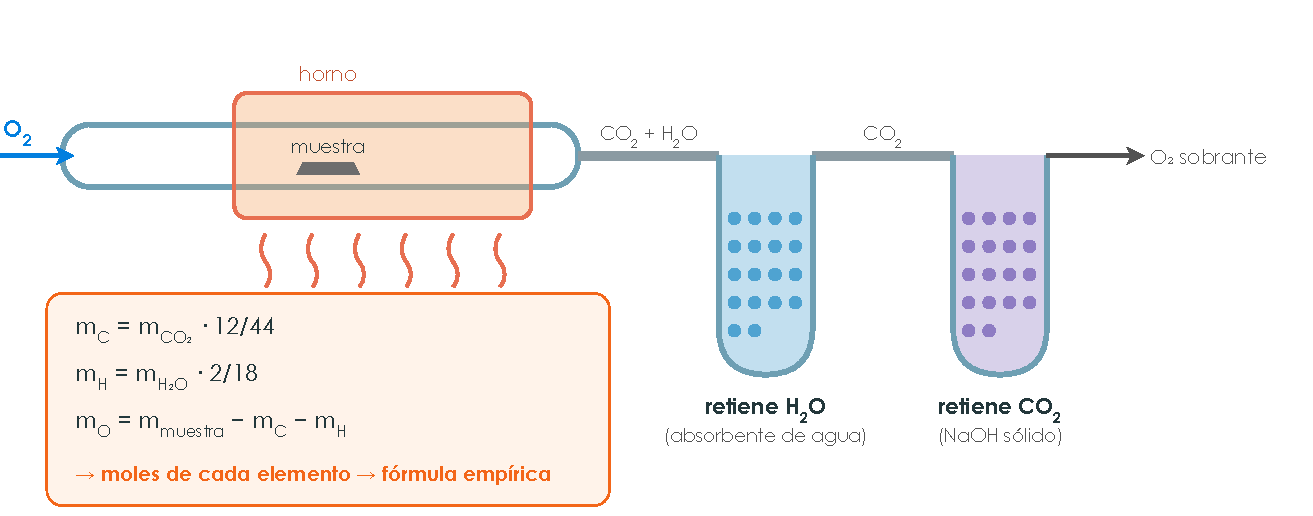
\includegraphics[width=0.85\linewidth]{FigurasSVG/UD0_Conocimientos_Basicos/pdf/UD0_E03_analisis_combustion.pdf}
        \caption{Análisis elemental por combustión}
        \label{fig:analisis-combustion}
    \end{figure}
    \begin{solu}
        \[ m_C = 3,6 \si{\g \ch{CO2}} \cdot \dfrac{12}{44} = \qty{0,982}{\g} \qquad m_H = 1,96 \si{\g \ch{H2O}} \cdot \dfrac{2}{18} = \qty{0,218}{\g} \]
        Comprobamos: $0,982 + 0,218 = \qty{1,20}{\g}$, coincide con la masa inicial (no hay oxígeno en el compuesto).
        \[ n_C = \dfrac{0,982}{12} = 0,0818 \si{\mol} \qquad n_H = \dfrac{0,218}{1} = 0,218 \si{\mol} \]
        Dividiendo por el menor:
        \[ C: \dfrac{0,0818}{0,0818} = 1 \qquad H: \dfrac{0,218}{0,0818} = 2,66 \]
        Multiplicando por 3 para obtener enteros: $C = 3$, $H = 8$. Fórmula empírica:
        \[ \mathbf{\textcolor{blue}{\ch{C3H8}}} \]
    \end{solu}
\end{exercise}

\begin{exercise}
    Un compuesto A se descompone por el calor formando un compuesto B y dióxido de carbono. Al calentar 300 g de A se obtuvieron 132 g de CO2 y se sabe que B tiene un 28\%  de O. ¿ Cuál será el porcentaje de O que contiene el compuesto A?. Sol: 47,68 \%
    \begin{solu}
        1. \textbf{Masa de B:} Por conservación de la masa, $A \rightarrow B + CO_2$:
        \[ m_B = 300 - 132 = \qty{168}{\g} \]

        2. \textbf{Masa de oxígeno en cada fragmento:}
        \[ m_{O(\ch{CO2})} = 132 \si{\g} \cdot \dfrac{32}{44} = \qty{96}{\g} \]
        \[ m_{O(B)} = 168 \si{\g} \cdot 0,28 = \qty{47,04}{\g} \]

        3. \textbf{Masa total de oxígeno en A y su porcentaje:}
        \[ m_{O(A)} = 96 + 47,04 = \qty{143,04}{\g} \]
        \[ \%O_A = \dfrac{143,04}{300} \cdot 100 = \mathbf{\textcolor{blue}{47,68 \%}} \]
    \end{solu}
\end{exercise}

\begin{exercise}
    Por tostación del sulfuro de cinc se obtiene el óxido del metal y se desprende dióxido de azufre. Si se dispone de 8,5 kg de sulfuro:
    a) ¿Qué cantidad de óxido se producirá?. b) ¿Con qué cantidad de oxígeno reacciona?
    Sol: a)  7.104 g de ZnO ; b) 4.189 g de oxígeno

    \begin{solu}
        \textbf{Reacción ajustada:} \ch{2 ZnS + 3 O2 -> 2 ZnO + 2 SO2}.

        1. \textbf{Moles de \ch{ZnS}:} $M_m(\ch{ZnS}) = 65,4 + 32 = \qty{97,4}{\g\per\mol}$.
        \[ n_{\ch{ZnS}} = \dfrac{8500}{97,4} = \qty{87,27}{\mol} \]

        a) \textbf{Masa de \ch{ZnO}:} Relación 1:1 con \ch{ZnS}. $M_m(\ch{ZnO}) = \qty{81,4}{\g\per\mol}$.
        \[ m_{\ch{ZnO}} = 87,27 \cdot 81,4 = \mathbf{\textcolor{blue}{\qty{7104}{\g}}} \]

        b) \textbf{Masa de \ch{O2}:} Relación 2:3 con \ch{ZnS}.
        \[ n_{\ch{O2}} = 87,27 \cdot \dfrac{3}{2} = \qty{130,9}{\mol} \]
        \[ m_{\ch{O2}} = 130,9 \cdot 32 = \mathbf{\textcolor{blue}{\qty{4189}{\g}}} \]
    \end{solu}
\end{exercise}

\begin{exercise}
    ¿ Qué masa de cloruro de plata puede obtenerse a partir de la reacción de 99,8 g de nitrato de plata con 35,4 g de cloruro de sodio?. Sol: 84,4 g
    \begin{solu}
        \textbf{Reacción:} \ch{AgNO3 + NaCl -> AgCl + NaNO3}.

        1. \textbf{Moles de cada reactivo:} $M_m(\ch{AgNO3}) = \qty{170}{\g\per\mol}$; $M_m(\ch{NaCl}) = \qty{58,5}{\g\per\mol}$.
        \[ n_{\ch{AgNO3}} = \dfrac{99,8}{170} = 0,587 \si{\mol} \qquad n_{\ch{NaCl}} = \dfrac{35,4}{58,5} = 0,605 \si{\mol} \]

        2. \textbf{Reactivo limitante:} Relación estequiométrica 1:1, luego \ch{AgNO3} (0,587 mol) es el limitante.

        3. \textbf{Masa de \ch{AgCl}:} $M_m(\ch{AgCl}) = \qty{143,4}{\g\per\mol}$.
        \[ m_{\ch{AgCl}} = 0,587 \cdot 143,4 = \mathbf{\textcolor{blue}{\qty{84,2}{\g}}} \]
    \end{solu}
\end{exercise}

\begin{exercise}
    ¿Cuántos \unit{\ml} de ácido clorhídrico del 25\% en peso y densidad \qty{0.91}{\gpml}  son necesarios para neutralizar \qty{32}{\g} de \ch{Ca(OH)2}. Sol: \qty{138.6}{\mL}
    \begin{solu}
        \ch{Ca(OH)2 + 2 HCl -> CaCl2 + 2 H2O}.
        \[ V = 32 \si{\g \ch{Ca(OH)2}} \cdot \dfrac{1 \si{\mol}}{74} \cdot \dfrac{2 \si{\mol \ch{HCl}}}{1 \si{\mol \ch{base}}} \cdot \dfrac{36,5 \si{\g}}{1 \si{\mol}} \cdot \dfrac{100 \si{\g \text{ dis.}}}{25 \si{\g \text{ ac.}}} \cdot \dfrac{1 \si{\mL}}{0,91 \si{\g}} = \mathbf{\textcolor{blue}{\qty{138,6}{\mL}}} \]
    \end{solu}
\end{exercise}

\begin{exercise}
    a) ¿Cuántos litros de oxígeno, medido en c.n., se necesitan para quemar \qty{36}{\g} de butano?. b) ¿Cuántos litros de \ch{CO2}, medidos en c.n., y cuántos gramos de agua se formarán?. Sol: a) \qty{90.4}{\L} de \ch{O}2. b) \qty{55.61}{\L} de \ch{CO2} y \qty{55.9}{\g} de agua.
    \begin{solu}
        1. \textbf{Reacción ajustada:} \( \ch{C4H10 + 13/2 O2 -> 4 CO2 + 5 H2O} \). \\
        2. \textbf{Moles de butano:} \( M(\ch{C4H10}) = \qty{58}{\g\per\mol} \). \\
        \( n = \dfrac{36}{58} = \qty{0,6207}{\mol} \). \\
        3. \textbf{Apartado a):} \\
        \( n_{\ch{O2}} = 0,6207 \cdot 6,5 = \qty{4,034}{\mol} \). \\
        \( V_{\ch{O2}} = 4,034 \si{\mol} \cdot 22,4 \si{\L\per\mol} = \textbf{\textcolor{blue}{\qty{90,37}{\L}}} \). \\
        4. \textbf{Apartado b):} \\
        \( V_{\ch{CO2}} = 0,6207 \cdot 4 \cdot 22,4 = \textbf{\textcolor{blue}{\qty{55,61}{\L}}} \). \\
        \( m_{\ch{H2O}} = 0,6207 \cdot 5 \cdot 18 = \textbf{\textcolor{blue}{\qty{55,86}{\g}}} \).
    \end{solu}

\end{exercise}

\begin{exercise}
    Halla el volumen de hidrógeno medido sobre agua, a \qty{25}{\celsius} y \qty{750}{\mmhg}, que se desprende al calentar \qty{1.52}{\g} de silicio con disolución de sosa cáustica, sabiendo que la presión de vapor del agua a \qty{25}{\celsius} es de \qty{23.8}{\mmhg} y que la reacción que tiene lugar es:
    \begin{reaction*}
        Si + 4 NaOH ->2 H2 + Na4SiO4
    \end{reaction*}
    Sol: \qty{2.77}{\L}
    \begin{figure}[H]
        \centering
        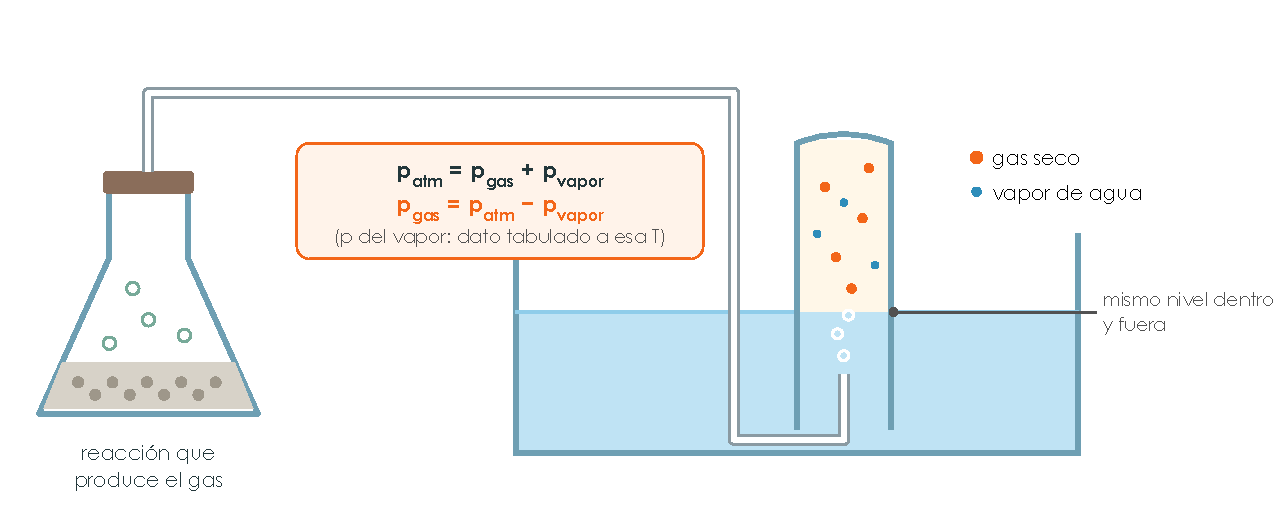
\includegraphics[width=0.8\linewidth]{FigurasSVG/UD0_Conocimientos_Basicos/pdf/UD0_E02_gas_sobre_agua.pdf}
        \caption{Gas recogido sobre agua}
        \label{fig:gas-sobre-agua}
    \end{figure}

    \begin{solu}
        1. \textbf{Moles de Si:} \( M(\text{Si}) = \qty{28,1}{\g\per\mol} \). \\
        \( n_{\text{Si}} = \dfrac{1,52}{28,1} = \qty{0,0541}{\mol} \). \\
        2. \textbf{Moles de \( \ch{H2} \):} Por estequiometría (1:2), \( n_{\ch{H2}} = 0,0541 \cdot 2 = \qty{0,1082}{\mol} \). \\
        3. \textbf{Presión del gas seco:} \( P_{\ch{H2}} = P_{total} - P_v = 750 - 23,8 = \qty{726,2}{\mmHg} = \qty{0,9555}{\atm} \). \\
        4. \textbf{Cálculo del volumen:} \\
        \( V = \dfrac{nRT}{P} = \dfrac{0,1082 \cdot 0,082 \cdot 298}{0,9555} = \textbf{\textcolor{blue}{\qty{2,77}{\L}}} \).
    \end{solu}

\end{exercise}

\begin{exercise}
    Halla la pureza de una muestra de sulfato de amonio, de la que tomados \qty{13.162}{\g} y tratados con exceso de sosa cáustica hacen desprender \qty{3.77}{\L}de amoniaco, medidos a \qty{18}{\celsius} y \qty{742}{\mmhg}, si además se origina sulfato de sodio y agua. Sol: 77,3\%

    \begin{solu}
        1. \textbf{Reacción:} \( \ch{(NH4)2SO4 + 2 NaOH -> 2 NH3 + Na2SO4 + 2 H2O} \). \\
        2. \textbf{Moles de \( \ch{NH3} \):} \( P = \dfrac{742}{760} = \qty{0,9763}{\atm} \); \( T = \qty{291}{\K} \). \\
        \( n_{\ch{NH3}} = \dfrac{0,9763 \cdot 3,77}{0,082 \cdot 291} = \qty{0,1544}{\mol} \). \\
        3. \textbf{Masa de \( \ch{(NH4)2SO4} \) pura:} (Relación 1:2) \\
        \( n_{sulfate} = \dfrac{0,1544}{2} = \qty{0,0772}{\mol} \). \\
        \( m_{puro} = 0,0772 \cdot 132,1 = \qty{10,198}{\g} \). \\
        4. \textbf{Pureza:} \( \% = \dfrac{10,198}{13,162} \cdot 100 = \textbf{\textcolor{blue}{77,5 \%}} \).
    \end{solu}

\end{exercise}

\begin{exercise}
    Calcula la pureza de una muestra de carburo cálcico (\ch{CaC2}) sabiendo que al tratar \qty{2.056}{\g} de carburo con agua se obtienen \qty{656}{\cc} de acetileno medidos sobre agua a \qty{22}{\celsius} y \qty{748}{\mmhg}. La presión de vapor del agua a \qty{22}{\celsius} es de \qty{19.8}{\mmhg}.
    \begin{reaction*}
        CaC2 + H2O -> C2H2 + Ca(OH)2.
    \end{reaction*}
    Sol: 81 \%
    \begin{solu}
        1. \textbf{Presión gas seco:} \( P = 748 - 19,8 = \qty{728,2}{\mmHg} = \qty{0,958}{\atm} \). \\
        2. \textbf{Moles de \( \ch{C2H2} \):} \( T = \qty{295}{\K} \); \( V = \qty{0,656}{\L} \). \\
        \( n = \dfrac{0,958 \cdot 0,656}{0,082 \cdot 295} = \qty{0,026}{\mol} \). \\
        3. \textbf{Masa de \( \ch{CaC2} \) pura:} (Relación 1:1) \\
        \( m_{puro} = 0,026 \si{\mol} \cdot 64,1 \si{\g\per\mol} = \qty{1,666}{\g} \). \\
        4. \textbf{Pureza:} \( \% = \dfrac{1,666}{2,056} \cdot 100 = \textbf{\textcolor{blue}{81,03 \%}} \).
    \end{solu}

\end{exercise}

\begin{exercise}
    Calcula la cantidad de caliza cuya riqueza en carbonato cálcico es del 85,3\%, que se necesita para obtener, por reacción con un exceso de ácido clorhídrico, \qty{10}{\L} de dióxido de carbono, medido a \qty{18}{\celsius} y \qty{752}{\mmhg}. Sol: \qty{48.6}{\g}
    \begin{solu}
        1. \textbf{Moles de \( \ch{CO2} \):} \( P = \dfrac{752}{760} = \qty{0,9895}{\atm} \); \( T = \qty{291}{\K} \). \\
        \( n = \dfrac{0,9895 \cdot 10}{0,082 \cdot 291} = \qty{0,415}{\mol} \). \\
        2. \textbf{Masa de \( \ch{CaCO3} \):} \( m = 0,415 \si{\mol} \cdot 100 \si{\g\per\mol} = \qty{41,5}{\g} \). \\
        3. \textbf{Masa de caliza:} \\
        \( m_{caliza} = \dfrac{41,5}{0,853} = \textbf{\textcolor{blue}{\qty{48,65}{\g}}} \).
    \end{solu}
\end{exercise}

\begin{exercise}
    ¿Cuántos gramos de cobre se obtendrán cuando el gas hidrógeno obtenido al hacer reaccionar \qty{41.6}{\g} de Al con un exceso de cloruro de hidrógeno se hace pasar sobre una cantidad en exceso de \ch{CuO}?. Las reacciones químicas son:
    \begin{reaction*}
        Al + HCl -> H2 + AlCl3
    \end{reaction*}
    \begin{reaction*}
        H2 + CuO -> Cu + H2O
    \end{reaction*}
    Sol: \qty{147}{\g}

    \begin{solu}
        1. \textbf{Moles de Al:} \( n = \dfrac{41,6}{27} = \qty{1,541}{\mol} \). \\
        2. \textbf{Moles de \( \ch{H2} \):} Ajuste \( \ch{2 Al + 6 HCl -> 2 AlCl3 + 3 H2} \). \\
        \( n_{\ch{H2}} = 1,541 \cdot \dfrac{3}{2} = \qty{2,3115}{\mol} \). \\
        3. \textbf{Moles de Cu:} Ajuste \( \ch{H2 + CuO -> Cu + H2O} \) (Relación 1:1). \\
        \( n_{\text{Cu}} = \qty{2,3115}{\mol} \). \\
        4. \textbf{Masa de Cu:} \( m = 2,3115 \si{\mol} \cdot 63,54 \si{\g\per\mol} = \textbf{\textcolor{blue}{\qty{146,87}{\g}}} \).
    \end{solu}

\end{exercise}

\begin{exercise}
    Una determinada cantidad de tricloruro de hierro ha sido oxidada completamente y todo el cloro se ha desprendido en forma de cloro. Este cloro gaseoso se ha empleado para transformar silicio en tetracloruro de silicio. Se han producido un total de \qty{7.44}{\mol} de tetracloruro de silicio. ¿Cuántos moles de tricloruro de hierro fueron oxidados?.
    \begin{reaction*}
        FeCl3 + O2 -> Cl2 + Fe2O3
    \end{reaction*}
    \begin{reaction*}
        Cl2 + Si -> SiCl4
    \end{reaction*}
    Sol: 9,92 moles
    \begin{solu}
        1. \textbf{Relación \( \ch{SiCl4} \) y \( \ch{Cl2} \):} \( \ch{Si + 2 Cl2 -> SiCl4} \). \\
        \( n_{\ch{Cl2}} = 7,44 \cdot 2 = \qty{14,88}{\mol} \). \\
        2. \textbf{Relación \( \ch{Cl2} \) y \( \ch{FeCl3} \):} \( \ch{4 FeCl3 + 3 O2 -> 2 Fe2O3 + 6 Cl2} \). \\
        Factor: \( 4 \si{\mol} \ch{FeCl3} \) producen \( 6 \si{\mol} \ch{Cl2} \). \\
        3. \textbf{Cálculo:} \\
        \( n_{\ch{FeCl3}} = 14,88 \si{\mol \ch{Cl2}} \cdot \dfrac{4 \si{\mol \ch{FeCl3}}}{6 \si{\mol \ch{Cl2}}} = \textbf{\textcolor{blue}{\qty{9,92}{\mol}}} \).
    \end{solu}

\end{exercise}

\begin{exercise}
    Se hace reaccionar 200 g de piedra caliza, que contiene un 60\% de carbonato cálcico con 200 cc de una disolución de ácido clorhídrico, de una concentración del 30\% (en peso) y densidad 1,15 g/ml. El proceso transcurre a 17ºC y 740 mmHg. Calcula: a) La masa de cloruro cálcico obtenido. b) el volumen de dióxido de carbono producido en las condiciones de la reacción. Sol: a) 104,9 g ,  b) 23,1 litros
    \begin{solu}
        \ch{CaCO3 + 2 HCl -> CaCl2 + CO2 + H2O}. \\
        $n_{\ch{CaCO3}} = \dfrac{200 \cdot 0,6}{100} = \qty{1,2}{\mol}$. $n_{\ch{HCl}} = \dfrac{200 \cdot 1,15 \cdot 0,3}{36,5} = \qty{1,89}{\mol}$. \\
        Limitante: \ch{HCl} (necesitaría 2,4 moles para todo el carbonato). \\
        a) $m_{\ch{CaCl2}} = \dfrac{1,89}{2} \cdot 111 = \mathbf{\textcolor{blue}{\qty{104,9}{\g}}}$. \\
        b) $V_{\ch{CO2}} = \dfrac{nRT}{P} = \dfrac{0,945 \cdot 0,082 \cdot 290}{740/760} = \mathbf{\textcolor{blue}{\qty{23,1}{\L}}}$.
    \end{solu}
\end{exercise}

\begin{exercise}
    En la valoración de 50 cc de una disolución de ácido sulfúrico se han gastado 37,6 cc de hidróxido de potasio 0,2 N. Halla su normalidad, así como los gramos de H2SO4 disueltos en los 50 cc. Sol: 0,15 N, 0,368 g
    \begin{solu}
        En una valoración ácido-base, en el punto de equivalencia los equivalentes de ácido y base coinciden: $N_{ac} \cdot V_{ac} = N_{base} \cdot V_{base}$.

        1. \textbf{Normalidad del ácido:}
        \[ N_{\ch{H2SO4}} = \dfrac{N_{base} \cdot V_{base}}{V_{ac}} = \dfrac{0,2 \cdot 37,6}{50} = \mathbf{\textcolor{blue}{0,15 \si{\normal}}} \]

        2. \textbf{Gramos de \ch{H2SO4} en los \qty{50}{\cc}:} Como \ch{H2SO4} tiene 2 hidrógenos, $M = N/2 = \qty{0,075}{\M}$. Equivalente-gramo $= M_m/2 = 98/2 = \qty{49}{\g}$.
        \[ n_{eq} = N \cdot V = 0,15 \si{\normal} \cdot 0,050 \si{\L} = 0,0075 \si{eq} \]
        \[ m = 0,0075 \si{eq} \cdot 49 \si{\g\per eq} = \mathbf{\textcolor{blue}{\qty{0,368}{\g}}} \]
    \end{solu}
\end{exercise}

\begin{exercise}
    Una muestra de 0,250 g de un ácido sólido se disolvió en agua y fue neutralizada exactamente por 40 cc de base 0,125 N. ¿ Cuánto vale el equivalente del ácido?. Sol: 50 g
    \begin{solu}
        En el punto de equivalencia, los equivalentes de ácido y base son iguales:
        \[ n_{eq,ac} = N_{base} \cdot V_{base} = 0,125 \si{\normal} \cdot 0,040 \si{\L} = \qty{0,005}{eq} \]
        El equivalente del ácido (masa por equivalente-gramo) es:
        \[ Eq = \dfrac{m_{ac}}{n_{eq}} = \dfrac{0,250 \si{\g}}{0,005 \si{eq}} = \mathbf{\textcolor{blue}{\qty{50}{\g\per eq}}} \]
    \end{solu}
\end{exercise}


\begin{exercise}
    El nitrógeno reacciona con el hidrógeno para formar amoniaco. ¿Qué volumen de amoniaco, medido a 27 ºC y 1,2 atm, se formarán al reaccionar 7 litros de nitrógeno, medidos en las mismas condiciones de P y T. ?. Sol: 14 l
    \begin{solu}
        \textbf{Reacción ajustada:} \ch{N2 + 3 H2 -> 2 NH3}.

        Al medirse los gases en las mismas condiciones de $P$ y $T$, la relación de volúmenes coincide con la relación estequiométrica molar (Ley de Avogadro): 1 volumen de \ch{N2} produce 2 volúmenes de \ch{NH3}.
        \[ V_{\ch{NH3}} = V_{\ch{N2}} \cdot \dfrac{2}{1} = \qty{7}{\L} \cdot 2 = \mathbf{\textcolor{blue}{\qty{14}{\L}}} \]
    \end{solu}
\end{exercise}


\begin{exercise}
    Se queman al aire 100 gramos de antracita, cuya riqueza en carbono es del 95\%. Calcula: a) el volumen de dióxido de carbono obtenido, medido en c.n.. b) el volumen de aire necesario para la combustión, sabiendo que el aire contiene un 21 \% de O2 en volumen. c) el volumen de dióxido de carbono obtenido, medido en c.n., suponiendo un rendimiento del 80\%. Sol: a) 177,3 l, b) 844,3 l, c) 141,84 l
    \begin{solu}
        \textbf{Reacción:} \ch{C + O2 -> CO2}.

        1. \textbf{Masa de carbono puro:} $m_C = 100 \cdot 0,95 = \qty{95}{\g}$.
        \[ n_C = \dfrac{95}{12} = \qty{7,917}{\mol} \]

        a) \textbf{Volumen de \ch{CO2} (c.n.):} Relación 1:1 con C.
        \[ V_{\ch{CO2}} = 7,917 \cdot 22,4 = \mathbf{\textcolor{blue}{\qty{177,3}{\L}}} \]

        b) \textbf{Volumen de aire necesario:} Relación 1:1 entre C y \ch{O2}, luego $n_{\ch{O2}} = \qty{7,917}{\mol}$ y $V_{\ch{O2}} = 7,917 \cdot 22,4 = \qty{177,3}{\L}$. Como el aire contiene 21\% de \ch{O2} en volumen:
        \[ V_{aire} = \dfrac{177,3}{0,21} = \mathbf{\textcolor{blue}{\qty{844,3}{\L}}} \]

        c) \textbf{Volumen de \ch{CO2} con rendimiento 80\%:}
        \[ V_{\ch{CO2}} = 177,3 \cdot 0,80 = \mathbf{\textcolor{blue}{\qty{141,84}{\L}}} \]
    \end{solu}
\end{exercise}

\begin{exercise}
    Se hacen reaccionar \qty{200}{\g} de una caliza que contiene un 60\% de carbonato cálcico con una disolución de ácido clorhídrico al 30\% en peso y densidad \qty{1.15}{\gpcc}. Calcula: a) volumen de \ch{CO2} obtenido, a \qty{18}{\celsius} y \qty{2}{\atm}. b) volumen de la disolución de ácido clorhídrico consumido. c) si en la práctica se obtuvieron \qty{100}{\g} de \ch{CaCl2}. ¿Cuál es el rendimiento de la reacción?. Sol: a) 14,31 l, b) 253,91 cm3, c) 75 \%
    \begin{solu}
        \textbf{Reacción:} \ch{CaCO3 + 2 HCl -> CaCl2 + CO2 + H2O}.

        1. \textbf{Moles de \ch{CaCO3} puro:} $m = 200 \cdot 0,60 = \qty{120}{\g}$.
        \[ n_{\ch{CaCO3}} = \dfrac{120}{100} = \qty{1,2}{\mol} \]
        (Se supone el \ch{HCl} en exceso, ya que no se indica su cantidad total, y el \ch{CaCO3} es el limitante.)

        a) \textbf{Volumen de \ch{CO2}:} Relación 1:1 con \ch{CaCO3}. $T = 18+273 = \qty{291}{\K}$.
        \[ V = \dfrac{nRT}{P} = \dfrac{1,2 \cdot 0,082 \cdot 291}{2} = \mathbf{\textcolor{blue}{\qty{14,31}{\L}}} \]

        b) \textbf{Volumen de \ch{HCl} consumido:} Relación 2:1 con \ch{CaCO3}.
        \[ n_{\ch{HCl}} = 1,2 \cdot 2 = \qty{2,4}{\mol} \]
        \[ V_{dis} = 2,4 \si{\mol} \cdot \dfrac{36,5 \si{\g}}{1 \si{\mol}} \cdot \dfrac{100 \si{\g\ dis.}}{30 \si{\g\ puro}} \cdot \dfrac{1 \si{\cc}}{1,15 \si{\g}} = \mathbf{\textcolor{blue}{\qty{253,91}{\cc}}} \]

        c) \textbf{Rendimiento:} Masa teórica de \ch{CaCl2} ($M_m = \qty{111}{\g\per\mol}$, relación 1:1 con \ch{CaCO3}):
        \[ m_{teor} = 1,2 \cdot 111 = \qty{133,2}{\g} \]
        \[ \% rendimiento = \dfrac{100}{133,2} \cdot 100 = \mathbf{\textcolor{blue}{75,1 \%}} \]
    \end{solu}
\end{exercise}

\subsection{Ejercicios EVAU}

\begin{exercise}
    En 1 kg de agua se disuelven 725 litros de gas amoniaco medidos a 20ºC y 744 mm de Hg. La densidad de la disolución obtenida es de 0,882 g/ml. Calcula: a) la concentración en g/l . b) la molaridad. c) la normalidad
    Sol: a) 295 g/l  ,   b) 17,35 M   ,   c) 17,35 N
    \begin{solu}
        $n_{\ch{NH3}} = \dfrac{(744/760) \cdot 725}{0,082 \cdot 293} = \qty{29,54}{\mol}$. \\
        Masa total = $1000 + (29,54 \cdot 17) = \qty{1502,2}{\g}$. \\
        $V_{dis} = \dfrac{1502,2}{0,882} = \qty{1703}{\mL}$. \\
        a) Conc: $\dfrac{29,54 \cdot 17}{1,703} = \mathbf{\textcolor{blue}{\qty{295}{\g\per\L}}}$. \\
        b) Molaridad: $\dfrac{29,54}{1,703} = \mathbf{\textcolor{blue}{\qty{17,35}{\M}}}$. \\
        c) Normalidad: $M=N$ para \ch{NH3}. \textbf{\textcolor{blue}{\qty{17,35}{\N}}}.
    \end{solu}
\end{exercise}

\begin{exercise}
    Cierta cantidad de hidrógeno recogido sobre agua a \qty{25}{\celsius} y \qty{737}{\mmhg} ocupa un volumen de \qty{245}{\mL}l. La presión de vapor de agua a esta temperatura es de 23,8 mm de Hg. Calcula el volumen de hidrógeno seco a 12 ºC y 770 mm de Hg. Sol: 217 ml
    \begin{solu}
        1. **Presión del gas seco:** Según la ley de Dalton, \( P_{total} = P_{H_2} + P_{v,H_2O} \). \\
        \( P_1 = 737 - 23,8 = \qty{713,2}{\mmHg} \). \\
        2. **Condiciones iniciales e ideales:** \\
        \( V_1 = \qty{245}{\mL} \), \( T_1 = 25 + 273 = \qty{298}{\K} \), \( P_1 = \qty{713,2}{\mmHg} \). \\
        3. **Condiciones finales:** \\
        \( P_2 = \qty{770}{\mmHg} \), \( T_2 = 12 + 273 = \qty{285}{\K} \). \\
        4. **Aplicación de la ley combinada de los gases:** \\
        \( \dfrac{P_1 \cdot V_1}{T_1} = \dfrac{P_2 \cdot V_2}{T_2} \Rightarrow V_2 = \dfrac{P_1 \cdot V_1 \cdot T_2}{P_2 \cdot T_1} \) \\
        \( V_2 = \dfrac{713,2 \cdot 245 \cdot 285}{770 \cdot 298} = \mathbf{\textcolor{blue}{\qty{217}{\mL}}} \)
    \end{solu}
\end{exercise}

\begin{exercise}
    Se dispone de una mezcla gaseosa formada por nitrógeno, oxígeno y dióxido de carbono que se encuentra a la presión de  \qty{700}{\mmhg} y a la temperatura de \qty{27}{\celsius}.
    Un análisis sobre la composición de la misma señaló que su contenido en peso era del 49\% de nitrógeno y del 40\% de oxígeno. Calcula: a) la presión parcial de cada uno de los gases. b) el volumen ocupado por \qty{100}{\g}  de la mezcla. c) la composición en volumen de la mezcla.
    Sol: a) \ch{N2}: \qty{376}{\mmhg}, \ch{O2}: \qty{269.2}{\mmhg}, \ch{CO2}:  \qty{53.9}{\mmhg}, b) \qty{86.8}{\L}
    c) \ch{N2}: \num{53,8}\%, \ch{O2}: \num{38,5}\%, \ch{CO2}: \num{7,7}\%

    \begin{solu}
        Tomamos una base de \( \qty{100}{\g} \)de mezcla: \\
        1. Cálculo de moles (\( n \)): \\
        \( n_{\ch{N2}} = \dfrac{49}{28} = \qty{1,75}{\mol} \). \\
        \( n_{\ch{O2}} = \dfrac{40}{32} = \qty{1,25}{\mol} \). \\
        \( n_{\ch{CO2}} = \dfrac{100 - (49+40)}{44} = \dfrac{11}{44} = \qty{0,25}{\mol} \). \\
        \( n_{total} = 1,75 + 1,25 + 0,25 = \qty{3,25}{\mol} \). \\
        2. Presiones parciales (\( P_i = \chi_i \cdot P_{total} \)): \\
        \( P_{\ch{N2}} = \dfrac{1,75}{3,25} \cdot 700 = \mathbf{\textcolor{blue}{\qty{376,9}{\mmHg}}} \). \\
        \( P_{\ch{O2}} = \dfrac{1,25}{3,25} \cdot 700 = \mathbf{\textcolor{blue}{\qty{269,2}{\mmHg}}} \). \\
        \( P_{\ch{CO2}} = \dfrac{0,25}{3,25} \cdot 700 = \mathbf{\textcolor{blue}{\qty{53,9}{\mmHg}}} \). \\
        3. Volumen total (\( V = \dfrac{nRT}{P} \)): \\
        \( V = \dfrac{3,25 \cdot 0,082 \cdot 300}{700/760} = \mathbf{\textcolor{blue}{\qty{86,8}{\L}}} \). \\
        4. Composición volumétrica (igual a \% molar): \\
        \( \%V_{\ch{N2}} = \dfrac{1,75}{3,25} \cdot 100 = \mathbf{\textcolor{blue}{53,8 \%}} \). \\
        \( \%V_{\ch{O2}} = \dfrac{1,25}{3,25} \cdot 100 = \mathbf{\textcolor{blue}{38,5 \%}} \). \\
        \( \%V_{\ch{CO2}} = \dfrac{0,25}{3,25} \cdot 100 = \mathbf{\textcolor{blue}{7,7 \%}} \).
    \end{solu}
\end{exercise}

\begin{exercise}
    Una muestra de \qty{0.580}{\g} de un compuesto orgánico, formado por carbono, hidrógeno y probablemente oxígeno, fue sometida a un proceso de combustión, obteniéndose \qty{1.274}{\g} de dióxido de carbono y \qty{0.696}{\g} de agua. Al volatilizar \qty{0.705}{\g} del compuesto, el gas que se produce, recogido sobre agua, ocupó un volumen de \qty{295}{\mL}, a \qty{27}{\celsius} y \qty{770}{\mmhg}. Calcula la fórmula del compuesto.
    Datos: Pv del agua = 26,7 mmHg;
    Sol: C3H8O

    \begin{solu}
        1. Masa de elementos en \( \qty{0,580}{\g} \): \\
        \( m_{\ch{C}} = 1,274 \si{\g \ch{CO2}} \cdot \dfrac{12}{44} = \qty{0,3475}{\g \ch{C}} \). \\
        \( m_{\ch{H}} = 0,696 \si{\g \ch{H2O}} \cdot \dfrac{2}{18} = \qty{0,0773}{\g \ch{H}} \). \\
        \( m_{\ch{O}} = 0,580 - 0,3475 - 0,0773 = \qty{0,1552}{\g \ch{O}} \). \\
        2. **Fórmula empírica:** \\
        \( n_{\ch{C}} = 0,0289 \); \( n_{\ch{H}} = 0,0773 \); \( n_{\ch{O}} = 0,0097 \). \\
        Dividiendo por el menor: \( \ch{C} \approx 3, \ch{H} \approx 8, \ch{O} = 1 \Rightarrow (\ch{C3H8O})_n \). \\
        3. **Masa molecular (\( M = \dfrac{mRT}{PV} \)):** \\
        \( P_{gas} = 770 - 26,7 = \qty{743,3}{\mmHg} = \qty{0,978}{\atm} \). \\
        \( M = \dfrac{0,705 \cdot 0,082 \cdot 300}{0,978 \cdot 0,295} = \qty{60,1}{\g\per\mol} \). \\
        Como \( M(\ch{C3H8O}) = 60 \), la fórmula es: \(\mathbf{\textcolor{blue}{\ch{C3H8O}}}\).
    \end{solu}
\end{exercise}

\begin{exercise}
    a) ¿Qué volumen de ácido sulfúrico (d = \qty{1.84}{\gpml} y del 96\% en peso) será necesario para disolver una muestra de  \qty{10}{\g} de cinc que contiene un 75\% de pureza?. b) ¿Cuántos gramos de sulfato de cinc se producirán?. c) ¿Cuántos litros de hidrógeno se desprenderán medidos a  \qty{740}{\mmhg} y \qty{37}{\celsius}?
    Sol: a) \qty{6.36}{\cc}, b) \qty{18.51}{\g}, c) \qty{3}{\L}.

    \begin{solu}
        Reacción: \( \ch{Zn + H2SO4 -> ZnSO4 + H2} \). \\
        Masa pura de \( \ch{Zn} = \qty{10}{\g} \cdot 0,75 = \qty{7,5}{\g} \). \\
        \( n_{\ch{Zn}} = \dfrac{7,5}{65,4} = \qty{0,1147}{\mol} \). \\
        a) **Volumen de ácido:** \\
        \( m_{ac. puro} = 0,1147 \si{\mol} \cdot 98 \si{\g\per\mol} = \qty{11,24}{\g} \). \\
        \( V_{dis} = \dfrac{11,24}{1,84 \cdot 0,96} = \mathbf{\textcolor{blue}{\qty{6,36}{\mL}}} \) (o \( \qty{6,36}{\cm^3} \)). \\
        b) **Masa de sulfato:** \\
        \( m_{\ch{ZnSO4}} = 0,1147 \si{\mol} \cdot 161,4 \si{\g\per\mol} = \mathbf{\textcolor{blue}{\qty{18,51}{\g}}} \). \\
        c) **Volumen de hidrógeno:** \\
        \( V = \dfrac{nRT}{P} = \dfrac{0,1147 \cdot 0,082 \cdot 310}{740/760} = \mathbf{\textcolor{blue}{\qty{3}{\L}}} \).
    \end{solu}

\end{exercise}



%----------------------------------------------------------------------------------------
%	PART
%----------------------------------------------------------------------------------------


    \part{Química Descriptiva}

%----------------------------------------------------------------------------------------
%	SECTIONING EXAMPLES CHAPTER
%----------------------------------------------------------------------------------------

    \chapterimage{orange3b.png} % Chapter heading image
    \chapterspaceabove{6.75cm} % Whitespace from the top of the page to the chapter title on chapter pages
    \chapterspacebelow{7.25cm} % Amount of vertical whitespace from the top margin to the start of the text on chapter pages

%------------------------------------------------


    \chapter{Estructura Atómica}

    \spacing{1.3}

\section{Introducción}
%Aunque los experimentos de Faraday sobre la electrolisis en 1830 sugirieron que el átomo estaba compuesto por cierto tipo de partículas, no fue hasta finales del siglo
%XIX cuando se comprobó la divisibilidad del átomo y su naturaleza eléctrica.
%Estos avances llegaron con el estudio de las descargas eléctricas sobre tubos de vacío, la radioactividad y los espectros atómicos.
Para estudiar la estructura atómica, es necesario establecer un modelo que nos permita tener una idea general de cómo está formado y qué partes lo componen; a esto lo llamamos \azuln{modelo atómico}.
% Así, los rayos catódicos descubiertos en 1886
% por Goldstein, el descubrimiento de los rayos catódicos en 1895 posteriormente identificados por J.J. Thomson como unas partículas cargadas a las que denominadas electrones;la radiactividad natural descubierta por Becquerel (1896), la cual permitió demostrar que todos los elementos químicos tendrán algo en común (partículas positivas, \(\alpha\), partículas negativas , \(\beta\), y radiación de muy alta energía) o el análisis espectroscópico descubierto por Bunsen en 1860 y mejorado por Balmer en 1885, trajeron consigo los primeros intentos por modelar al gran desconocido, el \textbf{átomo}.
% \section{Modelos atómicos}
\vspace{6pt}
\begin{definition}[Modelo atómico]
    Es una representación de la estructura del átomo que intenta explicar su comportamiento y propiedades.
\end{definition}
% A l largo de la historia se han ido proponiendo diferentes modelos atómicos. Los principales modelos atómicos propuestos se irán explicando en los siguientes apartados.


\section{Primeros modelos atómicos}

\subsection{Modelo atómico de Dalton}
El modelo atómico de Dalton se basaba en los siguientes postulados:
\begin{itemize}
    \item La materia está formada por partículas denominadas átomos.
    \item Todos los átomos de un mismo elemento son iguales.
    \item Los átomos son partículas muy pequeñas.
    \item Los átomos son partículas indivisibles.
    \item Dos o más átomos son iguales si tienen las mismas propiedades físicas y químicas.
    \item Dos o más átomos pueden unirse cuantitativamente para formar moléculas.
\end{itemize}
%    \begin{figure}[H]
%        \centering
%        \includegraphics[scale=0.3]{images/imagesUD1EstructuraAtomica/UD1_Teoria/dalton_atomic_model}
%        \caption{Modelo atómico de Dalton}
%        \label{fig:modelo_dalton}
%    \end{figure}

\subsection{Modelo de Thomson}\label{subsec:modelo-de-thomson}
Thomson pensaba que los átomos estaban constituidos por partículas más elementales y, a raíz del descubrimiento del electrón mediante el experimento con los rayos catódicos, postuló que:
\begin{itemize}
    \item El átomo es una masa de carga positiva en la que están incrustados los electrones.
    \item El átomo es neutro, tiene el mismo número de cargas positivas que de electrones.
\end{itemize}

Este modelo se conoce como \textbf{plum-pudding}, donde las cargas positivas estarían repartidas por todo el átomo y las negativas se encontrarían en unas posiciones fijas, pero en número suficiente para que el conjunto resultara neutro.

%    \begin{figure}[H]
%        \begin{subfigure}{0.45\linewidth}
%            \centering
%            \includegraphics[scale=1]{images/imagesUD1EstructuraAtomica/UD1_Teoria/Thomson_model.pdf}
%            %\caption{}
%            %\label{fig:}
%        \end{subfigure}
%        \hfill
%        \begin{subfigure}{0.45\linewidth}
%            \centering
%            \includegraphics[scale=0.5]{images/imagesUD1EstructuraAtomica/UD1_Teoria/thomson_model.jpeg}
%            \caption{Modelo atómico de Thomson}
%            %\label{fig:}
%        \end{subfigure}
%    \end{figure}
Este modelo explica la formación de iones positivos o negativos, la electricidad estática y la corriente eléctrica.
\begin{figure}[H]
    \centering
    \begin{subfigure}[b]{0.45\textwidth}
        \centering
        % [FIGURA ORIGINAL] \includegraphics[scale=0.2]{images/imagesUD1EstructuraAtomica/UD1_Teoria/dalton_atomic_model}
        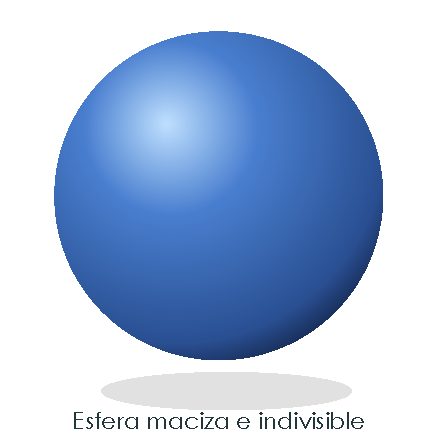
\includegraphics[width=0.75\linewidth]{FigurasSVG/UD1_Estructura_Atomica/pdf/UD1_01_modelo_dalton.pdf}
        \caption{Modelo atómico de Dalton}
        \label{fig:modelo_dalton}
    \end{subfigure}
    \hfill
    \begin{subfigure}[b]{0.45\textwidth}
        \centering
        % [FIGURA ORIGINAL] \includegraphics[scale=0.4]{images/imagesUD1EstructuraAtomica/UD1_Teoria/thomson_model.jpeg}
        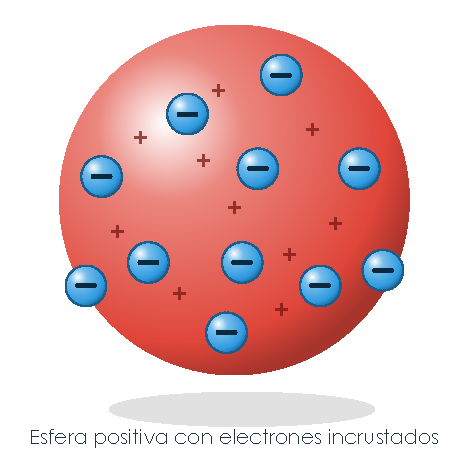
\includegraphics[width=0.8\linewidth]{FigurasSVG/UD1_Estructura_Atomica/pdf/UD1_02_modelo_thomson.pdf}
        \caption{Modelo atómico de Thomson}
        \label{fig:modelo_thomsom}
    \end{subfigure}
    \caption{Modelos atómicos de Dalton y Thomson}
    \label{fig:modelos_dalton_thomsom}
\end{figure}

\subsection{Modelo atómico de Rutherford}\label{subsec:modelo-atomico-de-rutherford}

Rutherford propuso el átomo formado por un núcleo y una periferia de electrones girando alrededor de este.
Este modelo se puede basar en los siguientes postulados:
\begin{itemize}
    \item El átomo tiene estructura planetaria.
    \item El átomo posee un núcleo central pequeño, con carga eléctrica positiva y que contiene casi toda la masa del átomo.
    \item Girando en órbitas circulares a grandes distancias alrededor del núcleo hay pequeñas masas con carga eléctrica negativa (los electrones).
    La atracción eléctrica entre los electrones y el núcleo es la fuerza centrípeta que permite a aquellos girar alrededor de este.
    \begin{centeredequation}
        F_e = F_c \Rightarrow K\ \dfrac{Q_n \cdot q_e}{r^2} = m_e\ \dfrac{v_e^2}{r}\label{eq:fuerzelectrica_fuerzacentripeta}
    \end{centeredequation}
    siendo:
    \begin{itemize}
        \item \(K = \text{Constante de Coulomb}\).
        En el vacío \(K = \SI{9e9}{\newton\square\metre\per\square\coulomb}\).
        \item \(Q_n\) es la carga del núcleo y depende del átomo.
        Se puede considerar como \(Q_n = Z\cdot q_e\) siendo \(Z\) el número atómico y, como la carga del protón es la misma en valor absoluto que la carga del electrón, se puede poner en función de esta.
        \item \(q_e\) es la carga del electrón, cuyo valor es de \qty{1.6e-19}{\coulomb}.
        \item \(r\) el radio de la órbita del electrón.
        \item \(m_e\) es la masa del electrón, cuyo valor es \qty{9.11e-31}{\kg}.
        \item \(v_e\) es la velocidad del electrón.
    \end{itemize}
    \item La suma de las cargas eléctricas negativas de los electrones debe ser igual a la carga positiva del núcleo, ya que el átomo es eléctricamente neutro.
    \item El átomo está prácticamente hueco.
\end{itemize}
\begin{figure}[H]
    \begin{subfigure}[c]{0.45\textwidth}
        \centering
        % [FIGURA ORIGINAL] \includegraphics[scale=0.25]{images/imagesUD1EstructuraAtomica/UD1_Teoria/rutherford_model_c}
        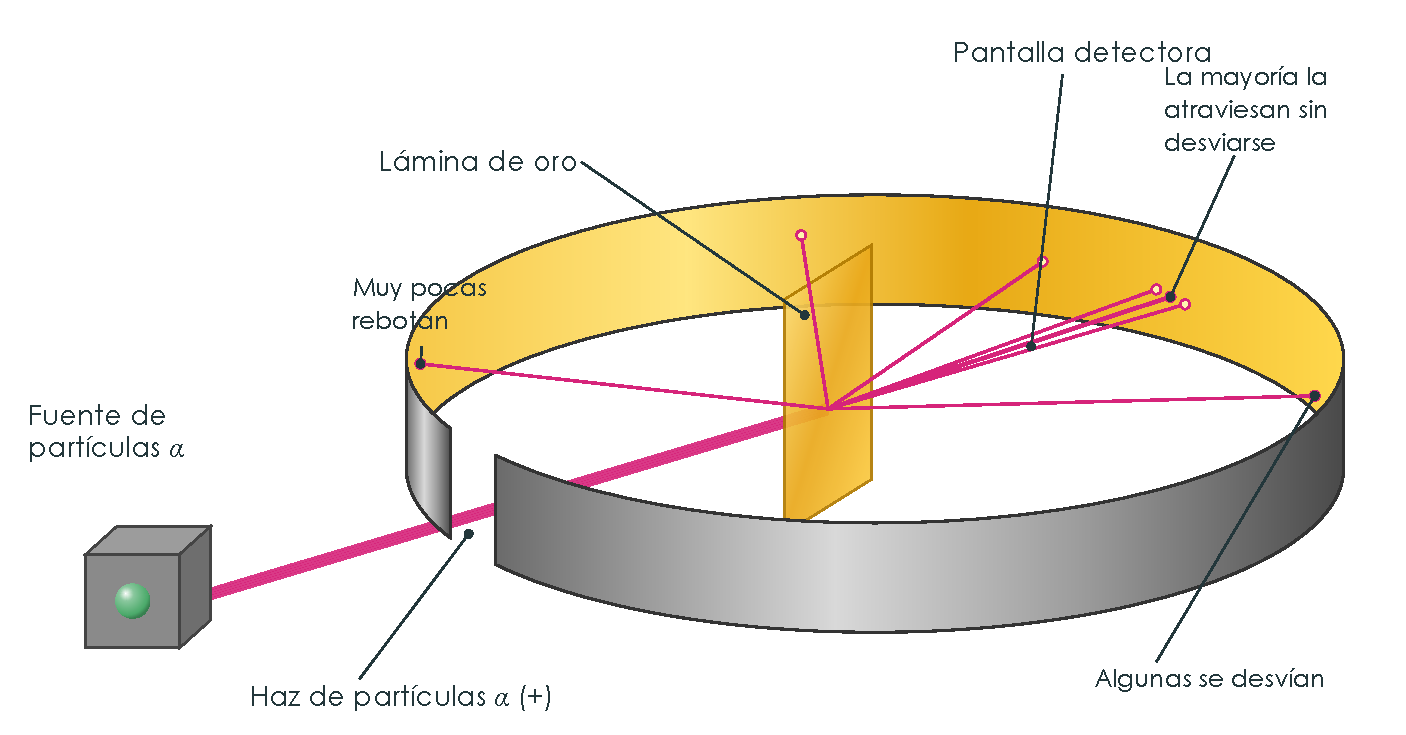
\includegraphics[width=1.0\linewidth]{FigurasSVG/UD1_Estructura_Atomica/pdf/UD1_03_experimento_rutherford.pdf}
        \caption{Experimento de Rutherford}
        \label{fig:experimento_rutherford}
    \end{subfigure}
    \hfill
    \begin{subfigure}[c]{0.45\textwidth}
        \centering
        % [FIGURA ORIGINAL] \includegraphics[scale=0.15]{images/imagesUD1EstructuraAtomica/UD1_Teoria/rutherford_model.png}
        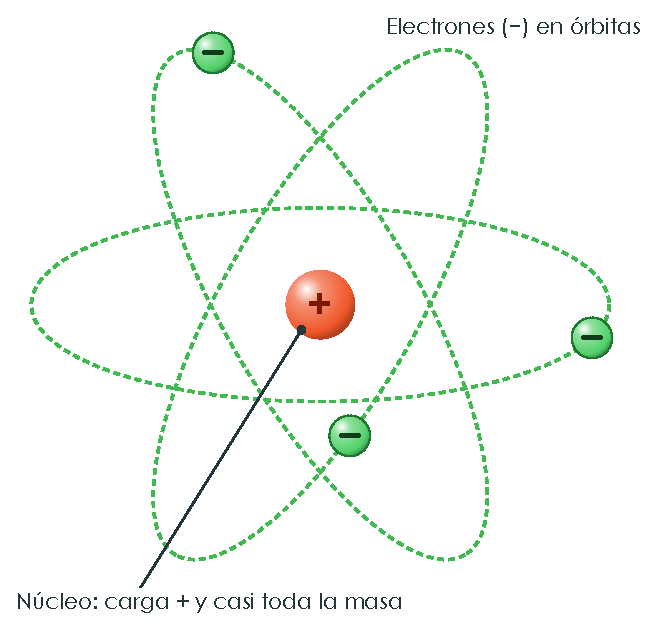
\includegraphics[width=0.85\linewidth]{FigurasSVG/UD1_Estructura_Atomica/pdf/UD1_04_modelo_rutherford.pdf}
        \caption{Modelo atómico de Rutherford}
        \label{fig:modelo_rutherford}
    \end{subfigure}
    \caption{Experimento y modelo atómico de Rutherford}
    \label{fig:experimento_modelo_rutherford}
\end{figure}
Para llegar a estas conclusiones, Rutherford se basó en un experimento en el que se hacía pasar partículas cargadas positivamente sobre una lámina de oro. La mayor parte de las partículas atravesaban la lámina del metal sin desviarse, por eso se propuso que el átomo estaba prácticamente hueco.
Solo una de cada \num{10000} chocaba contra el núcleo y rebotaba (\ref{fig:experimento_rutherford}).

En la figura \ref{fig:modelo_rutherford} tenemos la representación del modelo atómico de Rutherford.

\paragraph{Problemas o defectos del modelo de Rutherford:}

\begin{enumerate}[label=\numberballmDarkTeal]
        \item Una carga acelerada debería emitir ondas electromagnéticas y dicha emisión provocaría la pérdida de energía, lo que haría que el electrón describiera órbitas de radio decreciente hasta caer al núcleo.
        \item No daba explicación de los espectros atómicos.
        Según su modelo, los espectros serían continuos, algo que no sucede.
        Más adelante veremos lo que son los espectros de absorción y emisión.
\end{enumerate}


\section{Nuevos modelos atómicos}\label{sec:nuevos-modelos-atomicos}

\subsection{Modelo atómico de Bohr}\label{subsec:modelo-atomico-de-bohr}

El modelo atómico de Bohr se puede entender a partir de los siguientes postulados:

\begin{enumerate}[label=\numberballmDarkTeal]
        \item Los electrones giran en órbitas estables alrededor del núcleo.
        \item Las únicas órbitas permitidas por el electrón son las que cumplen:
        \begin{centeredequation}
            m_e\ v\ r = n\ \dfrac{h}{2\ \pi}
            \label{eq:cuantizacion_energia}
        \end{centeredequation}
        Donde \(\bm{n}\) solo puede tomar valores naturales (\(1,2,3,4,5\ \dots\)) y hace referencia al nivel energético, \(r\) es el radio de la órbita y \(h\) la constante de Planck.

        La expresión anterior viene de establecer que el momento angular está cuantizado, es decir, depende de números enteros de \(\hslash\).
        Donde:
        \begin{centeredequation}
            L = n\ \hslash \qquad \qquad \text{hay que tener en cuenta que: } \hslash = \dfrac{h}{2\pi}
        \end{centeredequation}
        \item Cuando un electrón pasa de una órbita superior a una órbita inferior, la diferencia de energía se emite en forma de energía electromagnética.

        La emisión o absorción de radiación electromagnética por los átomos se produce en forma de \azuln{cuantos}, unas diminutas cantidades elementales de energía según:
        \begin{centeredequation}
            \Delta E = h\;\nu
        \end{centeredequation}
        Si se produce el proceso inverso, de una órbita inferior a otra superior se absorbe energía.
        En ambos procesos la energía puesta en juego será:
        \begin{centeredequation}
            E_2-E_1 = h\;\nu
        \end{centeredequation}
        Siendo \(E_2\) la energía en la órbita final mientras que \(E_1\) será la energía en la órbita inicial.
\end{enumerate}
A partir de los postulados de Bohr podemos calcular:
\begin{enumerate}[label=\letraminuscula]
    % \item \textbf{Velocidad del electrón}. Estableciendo la condición de que el electrón realiza una trayectoria circular alrededor del núcleo tendremos que  $F_c=m\ a_c$. En este caso la fuerza centrípeta será la fuerza eléctrica lo que nos permite llegar a expresión:

    %     \begin{gather*}
    %         F_e = F_c \Rightarrow K\ \dfrac{Z \cdot q_e^2}{r^2} = m_e\ \dfrac{v_e^2}{r}\separ
    %         \kcoulomb\ \dfrac{Z \cdot q_e^2}{r^{\cancelred{2}}} =  m_e\ \dfrac{v_e^2}{\cancelred{r}}
    %     \end{gather*}
    %     despejando la velocidad de la última ecuación obtendríamos que:
    %     \begin{centeredequation}
    %         \tcboxmath[opteqA]{v^2 =  \dfrac{Q_n\  q_e}{m_e\ r}}
    %     \end{centeredequation}

    %     o bien

    %     \begin{centeredequation}
    %         \tcboxmath[opteqA]{v =\sqrt{ \dfrac{Q_n\  q_e}{m_e\ r}}}
    %     \end{centeredequation}
    \item \textbf{Velocidad del electrón}.
    Si tenemos en cuenta la ecuación \eqref{eq:cuantizacion_energia} podemos despejar la velocidad y obtendremos que:
    \begin{centeredequation}
        \tcboxmath[opteqA]{v = n\ \dfrac{h}{m_e\ 2 \pi\ r}}
        \label{eq:velocidad_electron}
    \end{centeredequation}
    \item \textbf{Cálculo del radio de las órbitas}:
    Si tenemos en cuenta la condición de que la fuerza de atracción electrostática entre el núcleo es igual a la que ejerce de fuerza centrípeta, podemos calcular el radio de la órbita del \el.
    Sabemos que la fuerza electroestática es:
    \begin{centeredequation}
        F_e = K\ \dfrac{Q_n\ q_e}{r^2}
    \end{centeredequation}
    Siendo \(K\) la constante de Coulomb, \(Q_n\) es la carga del núcleo y \(q_e\) la carga del electrón.
    Ya vimos anteriormente que la carga del núcleo la podemos escribir como \(Q_n = Z\ q_{proton}\) como la carga del protón y la carga del electrón es la misma, podemos decir que \(Q_n = Z\cdot q_e\).
    También sabemos que la fuerza centrípeta tiene la siguiente expresión:
    \begin{centeredequation}
        F_c = m_e\ \dfrac{v_e^2}{r}
    \end{centeredequation}
    Si igualamos la \(F_e\) y la \(F_c\) tendremos que:
    \begin{centeredequation}
        F_e = F_c \Rightarrow K\ \dfrac{Z \cdot q_e^2}{r^2} = m_e\ \dfrac{v_e^2}{r}
        \label{eq:centripeta_electrica}
    \end{centeredequation}
    y la ecuación \eqref{eq:velocidad_electron}, tras simplificar términos y despejar el radio llegamos a la expresión del radio.
    \begin{centeredequation}
        \begin{aligned}
            % F_e = F_c \Rightarrow K\ \dfrac{Q_n \cdot q_e}{r^2} = m_e\ \dfrac{v_e^2}{r}\separ
            K\ \dfrac{Q_n \cdot q_e}{r^2} = m_e\ n^2\ \dfrac{h^2}{4\pi^2\ m_e^2 \ r^3}\notag\separ
            \tcboxmath[opteqA]{r = n^2\ \dfrac{h^2}{4\pi^2\ m_e\ K\ Z\ q_e^2}}
        \end{aligned}
    \end{centeredequation}
    Debido a que \(h, m_e, K, q_e\) son constantes, podemos agruparlos en una nueva constante, denominada \(a\), que se corresponde al radio de la primera órbita de Bohr
    \begin{centeredequation}
        a = \dfrac{h^2}{4\pi^2\ m_e\ K\ Z\ q_e^2}
    \end{centeredequation}
    Por lo tanto, el radio de la órbita será:
    \begin{centeredequation}
        \tcboxmath[opteqA]{r = a\ n^2}
    \end{centeredequation}
    \item \textbf{Cálculo de la energía del electrón}: La energía total del electrón será la suma de la energía potencial eléctrica y la energía cinética debido al movimiento.
    \begin{centeredequation}
        E_T = E_p + E_c = -\kcoulomb\; \dfrac{Z\ q_e^2}{r} + \dfrac{1}{2}\; m_e\ v^2
        \label{eq:energiatotal}
    \end{centeredequation}
    De la ecuación \eqref{eq:centripeta_electrica} se deduce que:
    \begin{centeredequation}
        m_e\ v_e^2 = K\dfrac{Z\ q_e^2}{r}
    \end{centeredequation}
    Si esta última expresión la sustituimos en la ecuación \eqref{eq:energiatotal} tenemos que:
    \begin{centeredequation}
        E_T = -\dfrac{1}{2}\ K\ \dfrac{Z\ q_e^2}{r}
    \end{centeredequation}
    como \(K\) y \(q_e\) son constantes y como \(r = a\ n^2\) podemos escribir la última expresión como:
    \begin{centeredequation}
        E_T = -\dfrac{1}{2}\ K\ \dfrac{Z\ q_e^2}{a\ n^2} = - b \ \dfrac{1}{n^2}
    \end{centeredequation}
    siendo \(b = \dfrac{1}{2}\ K \dfrac{Z\ q_e^2}{a}\) quedando por tanto la energía total del electrón como:
    \begin{centeredequation}
        \tcboxmath[opteqA]{E_T = - b  \dfrac{1}{n^2}}
    \end{centeredequation}
    La constante \(\bm{b}\) coincide con el valor absoluto de la \textbf{energía de la primera órbita de Bohr} (\(n=1\)), que en el caso del átomo de hidrógeno tiene un valor de \energia[j]{-2.18e-18} que equivale a unos \energia[ev]{-13.6} ( \(\SI{1}{\electronvolt} =  \SI{1.6e-19}{\joule} \)).

    Por convenio de signos, el valor negativo significa que se trata de una \textbf{energía de estabilización}
    % Si en esta expresión se sustituye el valor de la velocidad y luego sustituimos el valor de $r$ la energía tendrá la forma:
    % \begin{centeredequation}
    %     E_T = -\dfrac{1}{n^2}\; \dfrac{m_eZ^2q_e^4}{8h^2\varepsilon_0^2}
    % \end{centeredequation}
    % Si al conjunto de todas estas constantes se engloba en una sola tendremos que
    % \begin{centeredequation}
    %     E_T = -\dfrac{1}{n^2}\;K^\prime
    % \end{centeredequation}
    \item \textbf{Cálculo de la diferencia de energía asociada entre dos órbitas}: Si un electrón pasa de una órbita $n_1$ a $n_2$ la variación de energía vendrá dada por:
    \begin{centeredequation}
        \Delta E = E_{2} - E_1 = b\ \left[\dfrac{1}{n_1^2} - \dfrac{1}{n_2^2} \right]
    \end{centeredequation}
    Si aplicamos que: $\Delta E = h\; \nu  \Rightarrow E_2-E_1 = h\; \nu \Rightarrow E_2-E_1= h\ \dfrac{c}{\lambda}$ tendremos que
    \begin{centeredequation}
        \Delta E = E_2 - E_1 =  b\  \biggl( \dfrac{1}{n_1^2} - \dfrac{1}{n_2^2} \biggr)  = h\ \dfrac{c}{\lambda}
    \end{centeredequation}
    despejando \(\dfrac{1}{\lambda}\) obtenemos la ecuación espectral derivada de la teoría de Bohr:
    \begin{centeredequation}
        \dfrac{1}{\lambda} = \dfrac{b}{h\ c}\biggl( \dfrac{1}{n_1^2} - \dfrac{1}{n_2^2} \biggr)
    \end{centeredequation}
    Ahora podemos comprobar que el factor constante, es decir \(\frac{b}{h\ c}\), es igual a la constante de Rydberg (ver ecuación \eqref{eq:ecucion_rydberg}). Para el átomo de hidrógeno:
    \begin{centeredequation}
        \dfrac{b}{h\ c} = \dfrac{\num{2.18e-18}}{\num{6.63e-34}\cdot \num{3e8}} = \SI{1.096e7}{\metre^{-1}}
    \end{centeredequation}
    % Si agregamos todas las constantes en una única constante $K^{\prime\prime}$
    % \begin{centeredequation}
    %     \nu = K^{\prime\prime}\; \left[\dfrac{1}{n_1^2} - \dfrac{1}{n_2^2} \right]
    % \end{centeredequation}
    % Si recordamos que $c = \lambda\;\nu$ se puede obtener la expresión:
    % \begin{centeredequation}
    %     \dfrac{1}{\lambda} = \dfrac{\nu}{c}= \dfrac{K^{\prime\prime}}{c}\; \left[\dfrac{1}{n_1^2} - \dfrac{1}{n_2^2} \right]
    % \end{centeredequation}
    % Si agrupamos todas las constantes en un única constante $R$ llamada contante de Rydberg tendremos que:
    % \begin{centeredequation}
    %     \tcboxmath[opteqA]{\dfrac{1}{\lambda} = R\; \left[\dfrac{1}{n_1^2} - \dfrac{1}{n_2^2} \right]}
    % \end{centeredequation}
    % Dando valores a $n_1$ y $n_2$ se obtienen las longitudes de onda de las series espectrales del hidrógeno (Lyman, Balmer, Paschen, Brackett, Pfund)
\end{enumerate}
De manera esquemática, el modelo atómico de Bohr lo podemos ver tal y como se muestra en la Figura \ref{fig:modelo_bohr}
\begin{figure}[H]
    \centering
    % [FIGURA ORIGINAL] \includegraphics[scale=0.3]{images/imagesUD1EstructuraAtomica/UD1_Teoria/modelo_bohr.jpeg}
    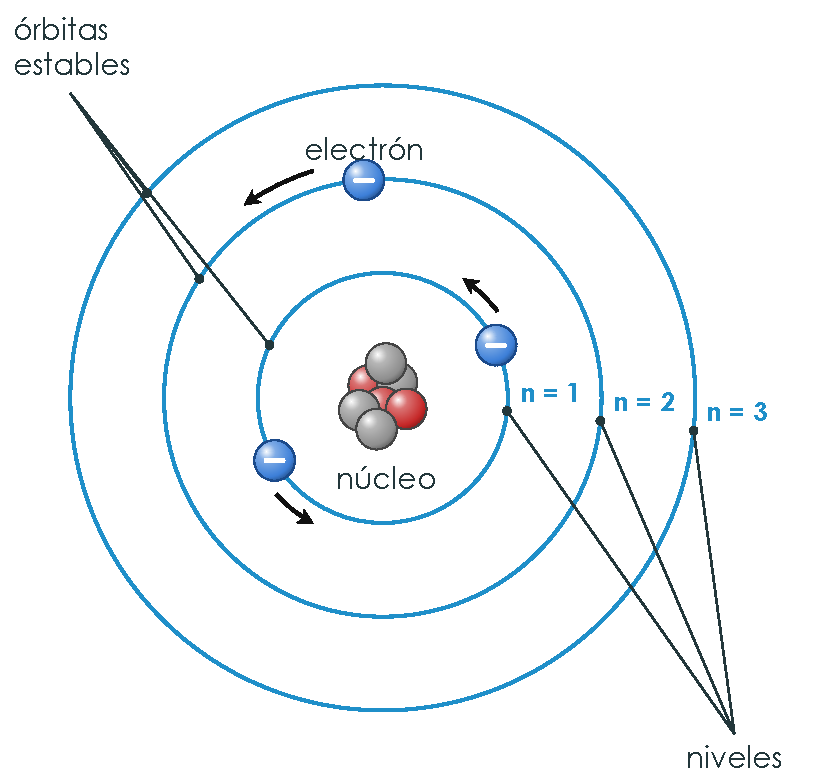
\includegraphics[width=0.5\linewidth]{FigurasSVG/UD1_Estructura_Atomica/pdf/UD1_05_modelo_bohr.pdf}
    \caption{Modelo atómico de Bohr}
    \label{fig:modelo_bohr}
\end{figure}

\paragraph{Aciertos del modelo de Bohr}
\begin{enumerate}[label=\numberballmDarkTeal]
        \item Permite deducir los radios de las órbitas.
        \item Permite deducir la fórmula que Balmer y Rydberg hallaron empíricamente.
        \item Esta deducción teórica proporciona unos valores de frecuencias y energías muy acordes con los hallados experimentalmente por los espectroscopistas.
\end{enumerate}
\paragraph{Limitaciones del modelo de Bohr}
\begin{enumerate}[label=\numberballmDarkTeal]
        \item Supone que las órbitas son circulares y no elípticas.
        \item Solo es aplicable de manera estricta al átomo de hidrógeno.
        \item Los avances en espectroscopia mostraron nuevas rayas que no se pueden explicar con este modelo.
\end{enumerate}

\subsection{Modelo atómico de Sommerfeld (Bohr-Sommerfeld)}

A medida que se iban mejorando las técnicas espectroscópicas, se fueron observando que las líneas espectrales eran en realidad \textbf{multipletes} es decir varias rayas juntas.
\begin{figure}[H]
    \centering
    % [FIGURA ORIGINAL] \includegraphics[scale=0.65]{images/imagesUD1EstructuraAtomica/UD1_Teoria/multipletes.PNG}
    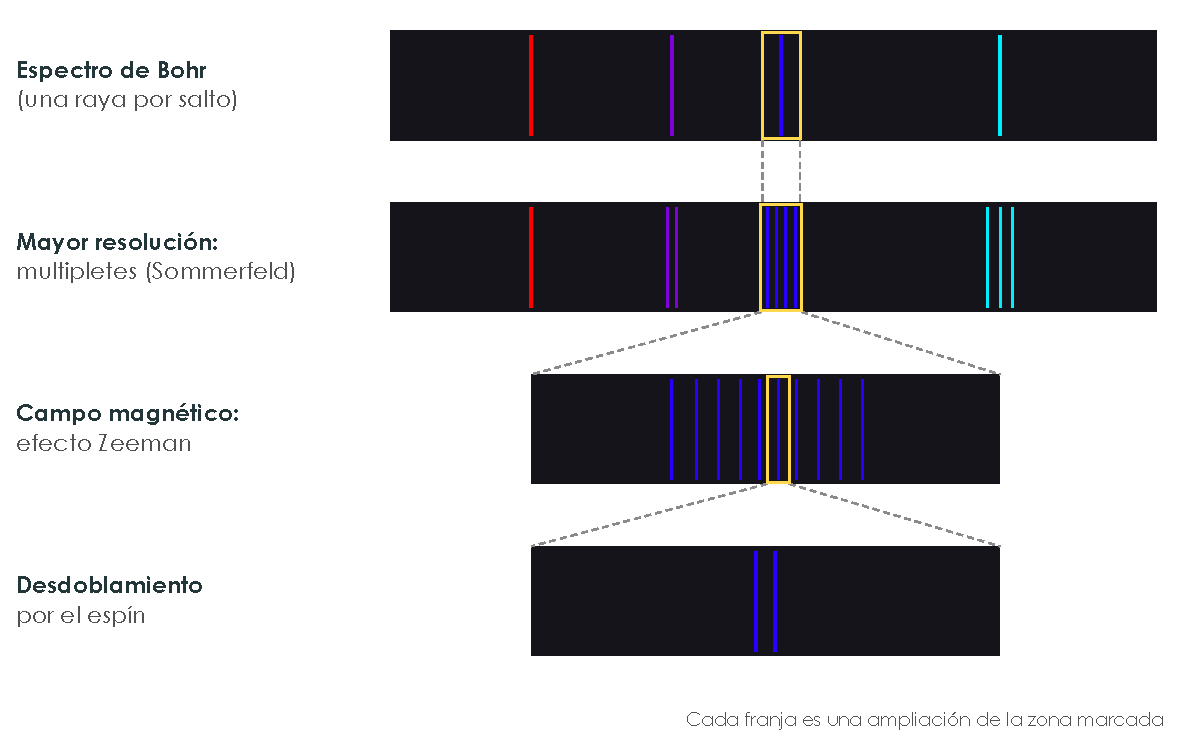
\includegraphics[width=0.7\linewidth]{FigurasSVG/UD1_Estructura_Atomica/pdf/UD1_06_multipletes.pdf}
    \caption{Desdoblamiento de las líneas espectrales}
    %\label{fig:}
\end{figure}
Sommerfeld propuso como explicación que cada órbita de Bohr, es decir cada nivel constaba en realidad de varias órbitas, o más exactamente de varios tipos de órbitas, que se diferenciaban en la forma en la que los electrones orbitaban alrededor del núcleo.
Supuso que siempre habría una órbita circular pero también órbitas elípticas con el núcleo situado en sus focos.

Matemáticamente, estas órbitas se representaban mediante un nuevo número cuántico  \(\bm{l}\) o también \(\bm{m_l}\) denominado \textbf{número cuántico secundario} o \textbf{azimutal}.
Los posibles valores de \(l\) van desde \(0 ... n-1\).
\begin{table}[H]
    \centering
    \caption{Nombre de los orbitales}
    \vspace{-5pt}
    \begin{tabular}{@{}ccc@{}}
        \toprule
        \textbf{Nº Cuántico} & \textbf{Orbital} & \textbf{Nombre} \\
        \bottomrule
        0                    & \(\bm{s}\)       & sharp \\[3pt]
        1                    & \(\bm{p}\)       & principal              \\[3pt]
        2                    & \(\bm{d}\)       & diffuse \\[3pt]
        3                    & \(\bm{f}\)       & fundamental     \\
        \bottomrule
    \end{tabular}
    \label{tab:nombre_orbitales}
\end{table}
%\begin{table}[H]
%    \centering
%    \begin{tblr}{
%        colspec = {Q[c,m]|Q[c,m]|Q[c,m]},
%        row{1} = {bg=mybluecolour, fg = white, font=\sffamily},
%        vlines = {1}{white},
%    }
%        \hline
%        \textbf{Nº. cuántico \(l\)} & \textbf{Órbita} & \textbf{Nombre} \\
%        \hline
%        0                           & \(\bm{s}\)      & sharp           \\
%        \hline
%        1                           & \(\bm{p}\)      & principal       \\
%        \hline
%        2                           & \(\bm{d}\)      & diffuse         \\
%        \hline
%        3                           & \(\bm{f}\)      & fundamental     \\
%        \hline
%    \end{tblr}
%\end{table}

\subsection{Modelo mecano-cuántico ondulatorio}

\textbf{Erwin Schrödinger} describió al electrón como una onda vibrando alrededor del núcleo y que estaba a su vez en todos los puntos de la órbita.

\begin{figure}[H]
    \centering
    % [FIGURA ORIGINAL] \includegraphics[scale=0.7]{images/imagesUD1EstructuraAtomica/UD1_Teoria/onda_atomo.PNG}
    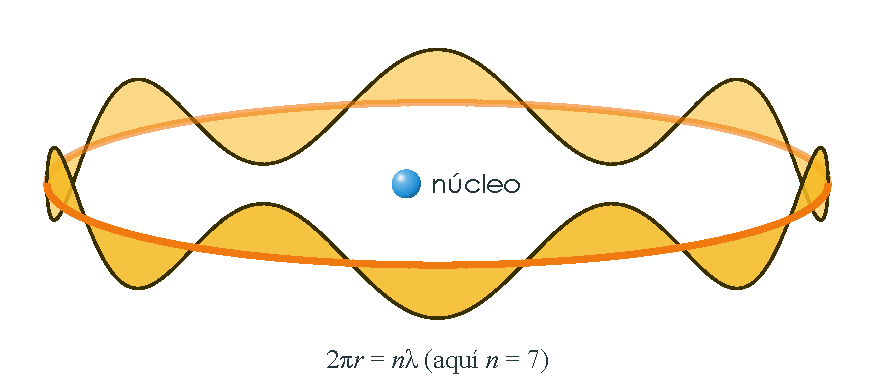
\includegraphics[width=0.6\linewidth]{FigurasSVG/UD1_Estructura_Atomica/pdf/UD1_07_onda_electron.pdf}
    \caption{}
    %\label{fig:}
\end{figure}
Schrödinger desarrolló una ecuación diferencial para obtener la función de onda \( \Psi \).
\begin{centeredequation}
    \dfrac{\delta^2\Psi}{\delta x^2} + \dfrac{\delta^2\Psi}{\delta y^2} + \dfrac{\delta^2\Psi}{\delta z^2} + \dfrac{8\pi^2m}{h^2}\;(E-V)\;\Psi = 0
\end{centeredequation}
\begin{enumerate}[label=\numberballmDarkTeal]
        \item $\Psi$ es la función de onda y no tiene por sí misma significado físico pero contiene información de la posición del electrón.
        Se le denomina también \blueremark{orbital}.
        \item El cuadrado de la función de onda $|\Psi|^2$ es la \textbf{densidad de probabilidad relativa del electrón} y representa la probabilidad de encontrar al electrón en un punto del espacio de coordenadas $(x, y, z)$
        \item \textbf{E}, la energía total del electrón.
        \item \textbf{V}, energía potencial el electrón.
\end{enumerate}
\begin{figure}[H]
    \centering
    % [FIGURA ORIGINAL] \includegraphics[scale=0.9]{images/imagesUD1EstructuraAtomica/UD1_Teoria/funciondeonda_distancia.PNG}
    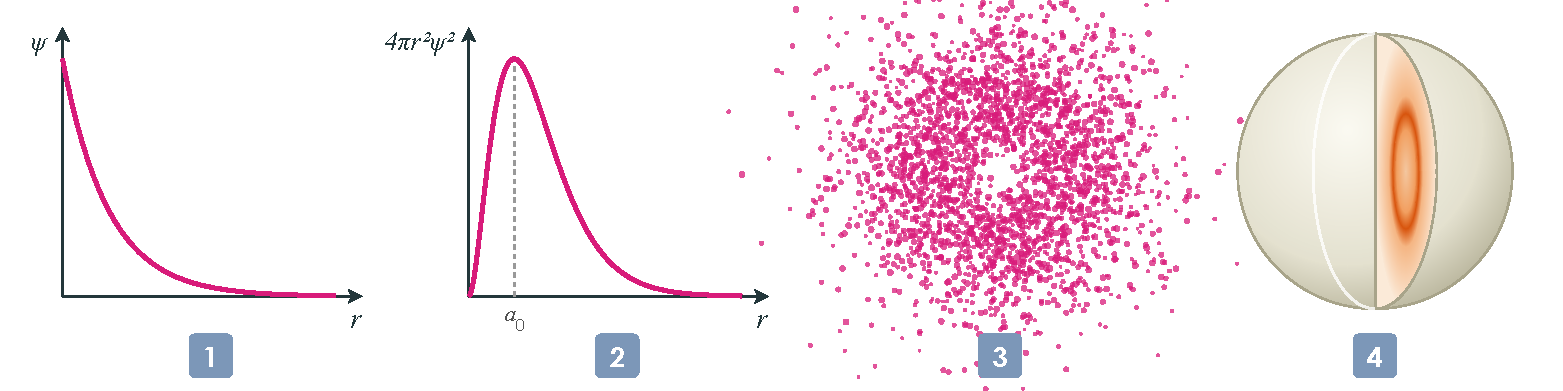
\includegraphics[width=1.0\linewidth]{FigurasSVG/UD1_Estructura_Atomica/pdf/UD1_08_funcion_onda_1s.pdf}
    \caption{1. Función de onda frente a la distancia con el núcleo. 2. Probabilidad de encontrar a un electrón frente a la distancia con el núcleo. 3. La probabilidad de encontrar al electrón en diferentes momentos. 4. Estructura espacial del orbital \(\bm{s}\)}
    %\label{fig:}
\end{figure}
Llegados a este punto, es importante conocer perfectamente el significado de órbita y de orbital.
\begin{itemize}
    \item \textbf{Órbita}: línea que describe el electrón en su movimiento alrededor del núcleo (Modelo de Bohr).
    \item \textbf{Orbital}: región en el espacio en la que hay probabilidad superior al 90\% de encontrar al electrón (Modelo mecánico ondulatorio).
\end{itemize}
% \subsubsection{Efecto Compton}

% Arthur Holly Compton, descubrió que algunos rayos X, al dispersarse a través de la materia, perdían energía y en consecuencia su longitud de onda aumentaba. La relación matemática entre la longitud de onda incidente y la resultante es:
% \begin{centeredequation}
%     \tcboxmath[opteqA]{\lambda = \lambda_0 + \; \dfrac{h}{m_e c}\; (1-\cos\theta)}
% \end{centeredequation}
% Donde:
% \begin{gather}
%     \lambda = \text{longitud de onda dispersada}\\\notag
%     \lambda_0 = \text{longitud de onda incidente}\\\notag
%     h = \text{constante de Plank }\SI{6,626e-34}{\joule\s}\\\notag
% \end{gather}

% \begin{gather}
%     m_e = \text{masa del electrón }\SI{9,109e-31}{\kilo\g}\\\notag
%     c = \text{velocidad de la luz } \SI{2,988e8}{\meter\per\s}\\\notag
%     \theta = \text{ángulo de dispersión}
% \end{gather}


\section{Bases experimentales de la mecánica cuántica}

Para entender los nuevos modelos atómicos indicados anteriormente, es necesario conocer algunas de las bases físicas que llevaron a su formulación.

\subsection{Teoría de Planck}\label{subsec:teoria-de-planck}

Planck llegó a la conclusión de que la radiación electromagnética (luz) no es un continuo, sino que se emite en forma de pequeños \textbf{paquetes} de energía, llamados cuantos de radiación o \textbf{fotones} cuya energía dependía de la frecuencia de la radiación según la ecuación.
\begin{definition}[Fotón]
    es un \textbf{cuanto} de radiación electromagnética o \textbf{cuanto de energía} y se trata de una partícula de energía en estado puro, que no tiene masa, según la siguiente ecuación:
    \begin{centeredequation}
        E = h\ \nu\label{eq:energia_relativista}
    \end{centeredequation}
    Siendo \(h\) la constante de Planck cuyo valor es \SI{6.63e-34}{\joule\s} y \(\nu\) la frecuencia de la radiación.
\end{definition}

La teoría de Planck es muy importante porque marca el inicio de la mecánica cuántica.

La energía de un fotón depende de su frecuencia: cuanto mayor sea esta, mayor será la energía que transporta. Sabemos que la frecuencia está relacionada con la longitud de onda según la expresión:
\begin{centeredequation*}
    c = \lambda\ \nu \longrightarrow \nu = \dfrac{c}{\lambda}
\end{centeredequation*}
Si lo sustituimos en la ecuación \eqref{eq:energia_relativista} tendremos que:

\begin{centeredequation}
    E = h\ \dfrac{c}{\lambda}
\end{centeredequation}

La \textbf{energía} de una radiación es la energía de cada uno de sus fotones, mientras que su \textbf{intensidad} viene determinada por el número de fotones.

La \textbf{frecuencia} (\(\nu\)) se mide en \unit{\hertz} (hercios), que equivale a \(1/\unit{\s}\), \si{\s^{-1}} o ciclos/s.

La \textbf{longitud de onda} (\(\lambda\)) se mide en unidades de longitud, como en \unit{\metre}, \unit{\nano\metre} o \unit{\angstrom} que equivale a \SI{e-10}{\metre}.

\subsection{Efecto fotoeléctrico}\label{subsec:efecto-fotoelectrico}

El efecto fotoeléctrico consiste en irradiar un material con una fuente de luz (onda).
La energía de la onda incidente se utiliza para arrancar y acelerar los electrones del material, siendo normalmente el material un metal.

\begin{definition}[Energía umbral o trabajo de extracción]
    Se representa con (\(W_0\)) o \( E_0 \) y es la energía justa para arrancar el electrón del metal, también se denomina \textbf{función de trabajo}, \textbf{trabajo de extracción} o \textbf{trabajo umbral} y es característica de cada metal o elemento.
\end{definition}

La energía aplicada durante el efecto fotoeléctrico sería igual a esa energía umbral o función de trabajo y la energía cinética máxima adquirida por dicho electrón.
El balance energético quedaría como:
\begin{centeredequation}
    E = W_0 + E_c\label{eq:efecto_fotoelectrico}
\end{centeredequation}
\begin{centeredequation}
    h\;\nu = W_0 + \dfrac{1}{2}\; m_e\; v_e^2 \label{eq:efecto_fotoelctrico_desarrollado}
\end{centeredequation}

\begin{consejo}[\textbf{Resolución de ejercicios sobre Efecto fotoeléctrico}]
    \phantom{a}

    \begin{enumerate}
        \item Debemos tener en cuenta que el trabajo umbral, también se llama función de trabajo o energía umbral y se representa con \(W_0\).
        \item Esta energía umbral, tendrá también una expresión del tipo: \(W_0 = h\cdot \nu_0\) donde \(\nu_0\) es la frecuencia que se necesita para arrancar un electrón.
        \item Debemos recordar que \(\nu_0\) se relaciona la longitud de onda (\(\lambda_0\)) según la expresión \(c = \lambda_0 \cdot \nu_0\).
        \item La energía \(E\) de la ecuación es la energía de la radiación incidente, si esa energía \(E < W_0 \) no se arrancará ningún electrón.
        \item Cuando me pidan la energía necesaria para arrancar un electrón, me están pidiendo esa energía umbral o trabajo umbral.
        \item Si me dan la longitud de onda o frecuencia, ya sea de la radiación incidente o de la energía umbral, me están dando la energía incidente o la energía umbral, ya que la podemos calcular según la ecuación: \( E = h\ \nu \) (ecuación \eqref{eq:energia_relativista}).
        \item La ecuación del efecto fotoeléctrico (ecuación \eqref{eq:efecto_fotoelectrico}) nos dice que, cuando se hace incidir una radiación de una determinada energía, esta energía primero se utilizará para arrancar el electrón, y si sobra energía, es decir, si la energía incidente es mayor que la energía umbral, lo que sobra se transforma en energía cinética, haciendo que el electrón adquiera una cierta velocidad.
    \end{enumerate}
\end{consejo}

A continuación veamos un posible ejemplo.

\begin{example}
    Calcula la frecuencia umbral y el trabajo de extracción del metal sodio, expresado en electronvoltios (\unit{\electronvolt}), sabiendo que al incidir sobre una superficie de dicho metal una radiación electromagnética cuya frecuencia es de \SI{1.18e15}{\hertz}, los electrones son arrancados con una energía cinética máxima de \energia[j]{4.18e-19}.
    Determina la velocidad máxima a la que salen los electrones.

        {\large{\negsubro{Solución:}}}

    Para evitar errores de cálculos, lo primero que debemos hacer es pasar todas unidades de las magnitudes a las correspondientes unidades del sistema internacional.

    Debemos recordar que el \si{\electronvolt} es una unidad de energía y por tanto debemos pasarla a \si{\joule}, el \si{\hertz} ya está en la unidad del sistema internacional porque equivale a \si{1\per\s}.

    En este caso como podemos ver, todo está en las unidades del sistema internacional.
    Lo primero que haremos es poner la fórmula del efecto fotoeléctrico donde \( E = W_0 + E_c\).
    Como nos piden que obtengamos el trabajo de extracción, lo que debemos hacer es despejar \(W_0\) y calcularlo:
    \begin{centeredequation}
        W_0 = E - E_c \rightarrow W_0 = h\ \nu - E_c =  (\num{6.63e-34}\cdot \num{1.18e15}) - \num{4.18e-19} \rightarrow W_0= \SI{3.64e-19}{\joule}
    \end{centeredequation}
    Como nos pide el trabajo de extracción en \unit{\electronvolt} lo que hacemos ahora es hacer el correspondiente cambio de unidades.
    \begin{centeredequation}
        \SI{3.64e-19}{\joule} \cdot \dfrac{\SI{1}{\electronvolt}}{\SI{1.6e-19}{\joule}} = \SI{2.28}{\electronvolt}
    \end{centeredequation}
    Ahora nos pide que calculemos la frecuencia umbral, si sabemos que \(W_ 0 = h\ \nu_0\) tan solo tenemos que despejar \( \nu_0 \) obteniendo que:
    \begin{centeredequation}
        \nu_0 = \dfrac{W_0}{h} \rightarrow \nu_0 = \dfrac{\num{3.64e-19}}{\num{6.63e-34}} \rightarrow \nu_0 = \SI{5.49e14}{\hertz}
    \end{centeredequation}
    También nos piden que calculemos la velocidad máxima de ese electrón, para ello sacaremos la velocidad de la energía cinética ya que nos dan su valor:
    \begin{gather*}
        E_c = \dfrac{1}{2}\ m_e \ v_e^2\separ
        v= \sqrt{\dfrac{2\ E_c}{m_e}} = \sqrt{\dfrac{2\cdot \num{4.18e-19}}{\num{9.1e-31}}} = \velocidad[ms]{9.6e5}
    \end{gather*}
    Quedando, por tanto, las soluciones como:
    \begin{centeredequation}
        \tcboxmath[opteqA]{W_0= \SI{2.28}{\electronvolt}} \qquad \tcboxmath[opteqA]{\nu_0= \SI{5.49e14}{\hertz}} \qquad \tcboxmath[opteqA]{v = \SI{9.6e5}{\mps}}
    \end{centeredequation}
\end{example}

\subsection{Espectros de absorción y de emisión}\label{subsec:espectros-de-absorcion-y-de-emision}

Los espectros de absorción o emisión se producen cuando existe la promoción de un electrón desde un orbital a otro.
Si durante este proceso se emite energía, tendremos un espectro de emisión y si absorbe energía tendremos un espectro de absorción.
\begin{itemize}
    \item \textbf{Espectros de absorción}: Se analiza la radiación absorbida por una muestra.
    Para ello se ilumina la muestra con una radiación compleja, por ejemplo luz blanca y luego se analiza la radiación obtenida tras irradiar la muestra.
    Los átomos de la muestra habrán absorbido algunas radiaciones (alguna parte del espectro electromagnético) y, por tanto, los electrones pasarán de un nivel inferior a otro nivel superior, puesto que ganan energía.
    Estas transiciones se observan con unas líneas negras que indican ese tránsito. Ver Figura \ref{fig:absorcion_atomica}.
%        \begin{figure}[H]
%            \centering
%            \includegraphics[scale=0.8]{images/imagesUD1EstructuraAtomica/UD1_Teoria/espectroelectromagnetico.PNG}
%            %\caption{}
%            %\label{fig:}
%        \end{figure}


%        \begin{figure}[H]
%            \centering
%            \includegraphics[scale=1]{images/imagesUD1EstructuraAtomica/UD1_Teoria/espectro_absorcion.PNG}
%            %\caption{}
%            %\label{fig:}
%        \end{figure}
    \item \textbf{Espectros de emisión}: en este caso se analiza la radiación emitida por una muestra sobre la cual no incide ninguna radiación externa. Algunos átomos emiten radiación de forma espontánea como sucede con los cuerpos fluorescentes mientras que los que no lo hacen tienen que ser excitados con una fuente de calor o eléctrica. Las emisiones de estos átomos se verán como unas líneas de color sobre un fondo negro indicando el paso de los electrones desde un nivel superior a un nivel inferior emitiendo, por tanto, energía. Ver Figura \ref{fig:emision_atomica}.
%        \begin{figure}[H]
%            \centering
%            \includegraphics[scale=1]{images/imagesUD1EstructuraAtomica/UD1_Teoria/espectro_emision.PNG}
%            %\caption{}
%            %\label{fig:}
%        \end{figure}
\end{itemize}

\begin{figure}[H]
    \centering
    \begin{subfigure}[b]{0.45\textwidth}
        \centering
        % [FIGURA ORIGINAL] \includegraphics[scale=0.75]{images/imagesUD1EstructuraAtomica/UD1_Teoria/espectro_absorcion_atomica}
        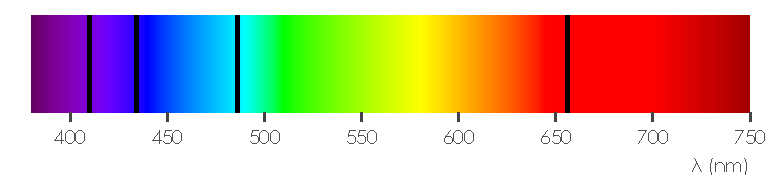
\includegraphics[width=1.0\linewidth]{FigurasSVG/UD1_Estructura_Atomica/pdf/UD1_09_espectro_absorcion_hidrogeno.pdf}
        \caption{Espectro de absorción atómica}
        \label{fig:absorcion_atomica}
    \end{subfigure}
    \hfill
    \begin{subfigure}[b]{0.45\textwidth}
        \centering
        % [FIGURA ORIGINAL] \includegraphics[scale=0.75]{images/imagesUD1EstructuraAtomica/UD1_Teoria/espectro_emision_atomica}
        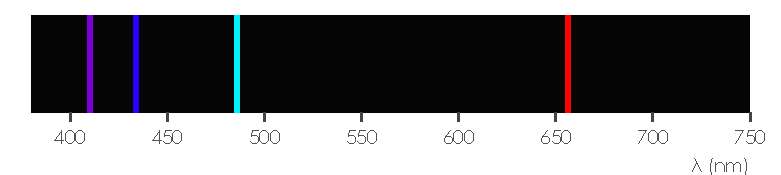
\includegraphics[width=1.0\linewidth]{FigurasSVG/UD1_Estructura_Atomica/pdf/UD1_10_espectro_emision_hidrogeno.pdf}
        \caption{Espectro emisión atómica}
        \label{fig:emision_atomica}
    \end{subfigure}
    \caption{Espectros de emisión y absorción atómica}
    \label{fig:emision_absorcion_atomica}
\end{figure}

\subsection{Series espectrales}

Las rayas obtenidas en los espectros de emisión y absorción podían obtenerse mediante una ecuación general llamada \textbf{fórmula de Rydberg}:
\begin{centeredequation}
    \dfrac{1}{\lambda} = R\ \biggl(\dfrac{1}{n_1^2} - \dfrac{1}{n_2^2} \biggr) \label{eq:ecucion_rydberg}
\end{centeredequation}
Siendo \(R\) la \textbf{constante de Rydberg} y tiene un valor de \SI{1.09677566e7}{\metre^{-1}} para el átomo de hidrógeno y \(n_1\) y \(n_2\) son los niveles energéticos en los que se producen el tránsito electrónico.
Son siempre números enteros que van desde el 1 hasta el 7.
El nivel energético menor siempre se asigna al \(n_1\) mientras que el nivel energético mayor a \(n_2\), ya que de la ecuación de Rydberg obtenemos la longitud de onda y esta debe ser siempre positiva.
Si tenemos un espectro de emisión, entonces le pondremos un signo negativo a la energía (desprende energía), y si tenemos un espectro de absorción, le pondremos un signo positivo a la energía (absorbe energía).

Tenemos principalmente 4 series espectrales cuyas fórmulas de Rydberg son las siguientes.
\vspace{-8pt}
\begin{multicols}{2}
    \begin{itemize}
        \item \textbf{Serie de Lyman}: \( \dfrac{1}{\lambda} = R\ \biggl(\dfrac{1}{1^2} - \dfrac{1}{n_2^2} \biggr)\)
        \item  \textbf{Serie de Balmer}: \( \dfrac{1}{\lambda} = R\ \biggl(\dfrac{1}{2^2} - \dfrac{1}{n_2^2} \biggr)\)
        \item  \textbf{Serie de Paschen}: \( \dfrac{1}{\lambda} = R\ \biggl(\dfrac{1}{3^2} - \dfrac{1}{n_2^2} \biggr)\)
        \item  \textbf{Serie de Brackett}: \( \dfrac{1}{\lambda} = R\ \biggl(\dfrac{1}{4^2} - \dfrac{1}{n_2^2} \biggr)\)
        \item \textbf{Serie de Pfund}: \( \dfrac{1}{\lambda} = R\ \biggl(\dfrac{1}{5^2} - \dfrac{1}{n_2^2} \biggr)\)
    \end{itemize}
\end{multicols}
Como podemos ver en las fórmulas la serie de Lyman, siempre parte o llega al nivel energético \(n = 1\), la de Balmer a \(n = 2\), la de Paschen a \(n = 3\), la de Brackett a \(n = 4\) y la de Pfund a \(n = 5\).
Estas series espectrales las podemos ver en la Figura \ref{fig:series_espectrales}.

\begin{figure}[H]
    \centering
    % [FIGURA ORIGINAL] \includegraphics[scale=1]{images/imagesUD1EstructuraAtomica/UD1_Teoria/series_espectrales}
    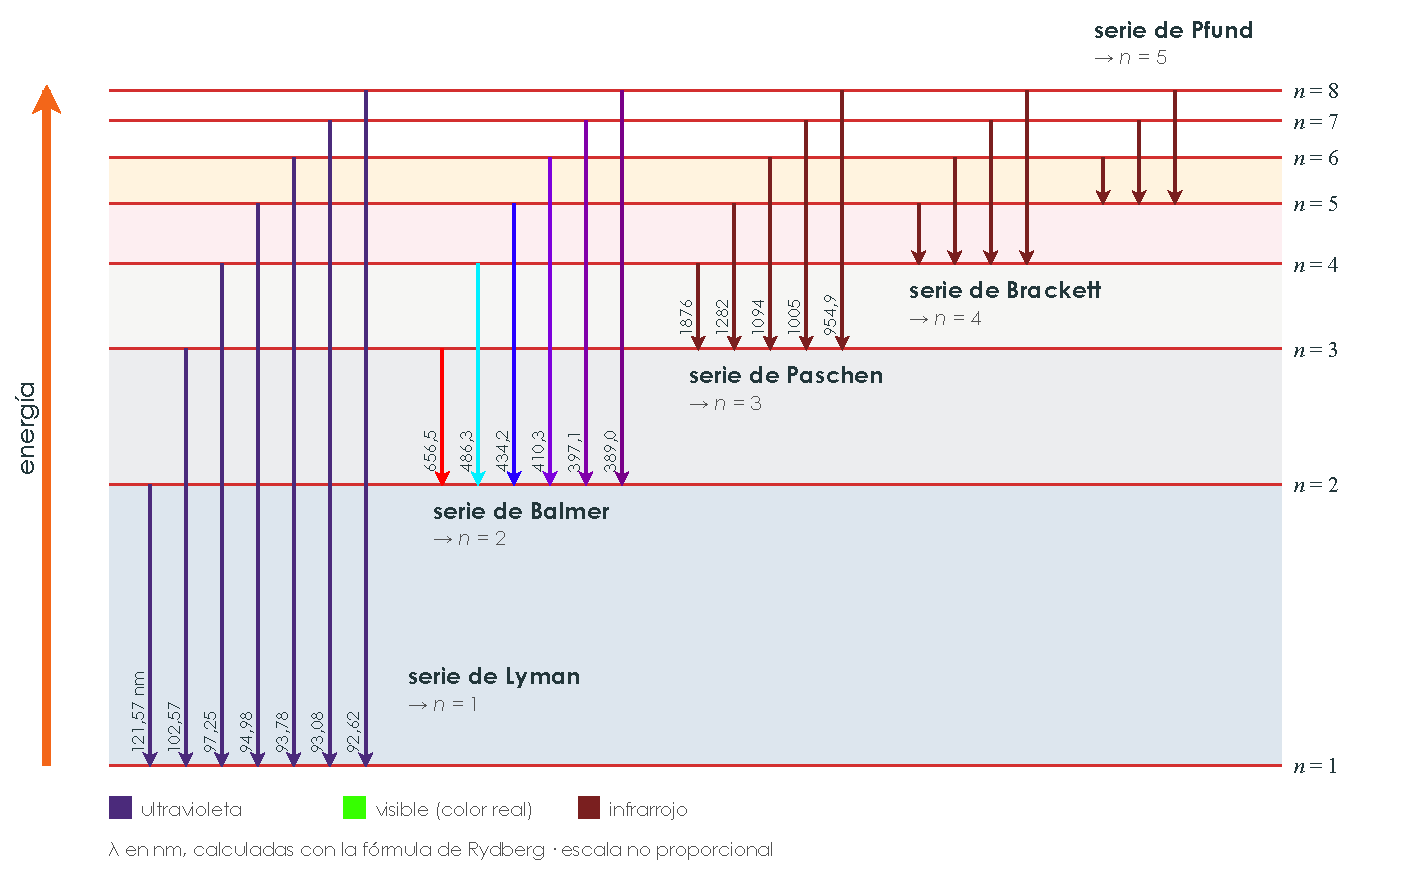
\includegraphics[width=0.9\linewidth]{FigurasSVG/UD1_Estructura_Atomica/pdf/UD1_11_series_espectrales.pdf}
    \caption{Series espectrales}
    \label{fig:series_espectrales}
\end{figure}

\subsection{Dualidad onda-corpúsculo. Principio de De Broglie}\label{subsec:dualidad-onda-corpusculo.-principio-de-de-broglie}
De Broglie recogió la idea de la naturaleza dual de la luz (se puede comportar como una onda y como un corpúsculo).

\begin{principio}[De Broglie]
    Las masas en movimiento se pueden comportar como ondas. Llegando a una expresión que relaciona la longitud de onda con la cantidad de movimiento según:
    \begin{centeredequation}
        \lambda = \dfrac{h}{p} \label{eq:debrolie}
    \end{centeredequation}
    Si tenemos en cuenta que \(p = m\ v\), la ecuación \eqref{eq:debrolie} quedaría como:
    \begin{centeredequation}
        \lambda = \dfrac{h}{mv} \label{eq:debrolie_desarrollada}
    \end{centeredequation}
    Siendo \(h\) la constante de Planck, \(v\) la velocidad de la partícula y \(m\) la masa de la partícula.
\end{principio}

\subsection{Principio de incertidumbre de Heisenberg}\label{subsec:principio-de-incertidumbre-de-heisenberg}

\begin{principio}[Principio de incertidumbre de Heisenberg]
    es imposible medir simultáneamente, y con precisión absoluta, el valor de dos variables conjugadas.
\end{principio}

Este principio establece que la precisión de la medida es limitada.
Si tomamos una única coordenada para la posición y la cantidad de movimiento podemos establecer la siguiente expresión:

\begin{centeredequation}
    \Delta x \cdot \Delta p_x \geq \dfrac{h}{4\pi} \label{eq:heisenberg}
\end{centeredequation}
Donde:
\begin{gather*}
    \Delta x = \text{indeterminación en la posición}\separ
    \Delta p_x = \text{indeterminación en el impulso}\separ
    h ( \text{Constante de Plank}) = \SI{6.63e-34}{\joule\s}
\end{gather*}


\section{Números cuánticos}\label{sec:numeros-cuanticos}

Al resolver la ecuación de Schrödinger se observó que solo se permitían ciertas energías porque las funciones de onda dependían de tres variables que solo podían tomar unos valores discretos.
Estas variables son los \textbf{números cuánticos} $\mathbf{n, l\; y\; m}$.
Posteriormente, \textbf{Paul Adrien Maurice Dirac} introdujo un número cuántico \textbf{spin \textit{s}}.

\begin{enumerate}[label=\numberballmDarkTeal]
        \item \textbf{\textit{n}} es el número cuántico principal, toma valores naturales excluido el cero $\bm{n} = 1, 2, 3, 4 \dots$.
        Este número cuántico determina el nivel energético.
        Determina la extensión espacial, cuanto mayor sea el valor de $n$ mayor será el orbital.
        \item \textbf{\textit{l}} es el número cuántico secundario o azimutal, toma valores $ l = 0 \dots n-1$.
        Determina la forma del orbital atómico.
        Siguiendo la terminología espectroscopista, los orbitales se designan como:
        \begin{enumerate}
            \item \textit{l} = 0.
            Orbital \blueremark{s} (sharp).
            Son esféricos.
            \begin{figure}[H]
                \centering
                % [FIGURA ORIGINAL] \includegraphics[scale=1]{images/imagesUD1EstructuraAtomica/UD1_Teoria/orbital_s}
                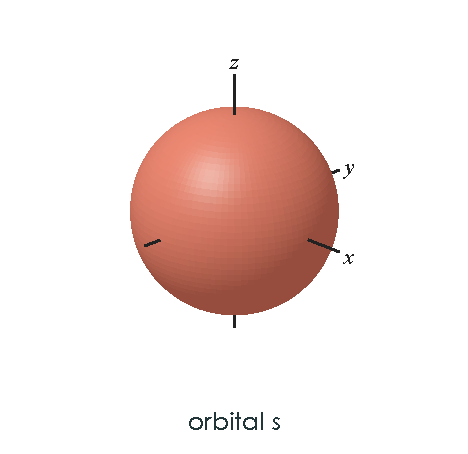
\includegraphics[width=0.3\linewidth]{FigurasSVG/UD1_Estructura_Atomica/pdf/UD1_12_orbital_s.pdf}
                \caption{Orbital \(\bm{s}\)}
                %\label{fig:}
            \end{figure}
            \item \textit{l} = 1.
            Orbital \blueremark{p} (principal).
            Presentan dos lóbulos idénticos a lo largo de un eje.
            La unión de ambos lóbulos coincide con el núcleo atómico.
            Tenemos tres orbitales tipo $p$: $p_x$, $p_y$, $p_z$.
            Cada uno de ellos llevará asociado un valor del número cuántico $m$ ($m=-1, m=0, m=+1$).
            \begin{figure}[H]
                \centering
                % [FIGURA ORIGINAL] \includegraphics[scale=0.6]{images/imagesUD1EstructuraAtomica/UD1_Teoria/orbital_p}
                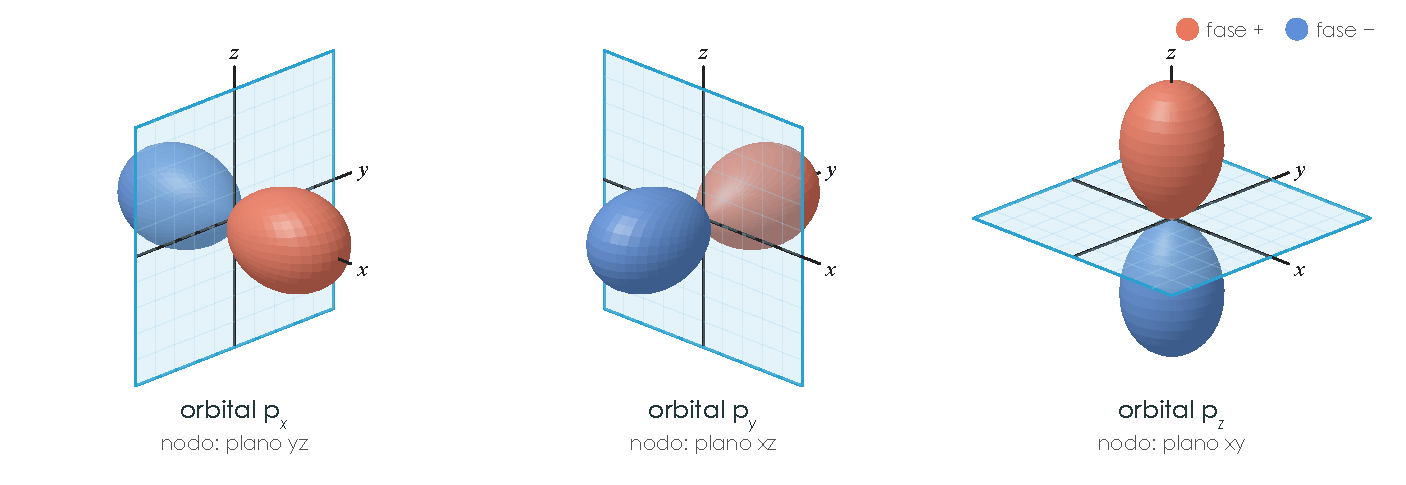
\includegraphics[width=0.9\linewidth]{FigurasSVG/UD1_Estructura_Atomica/pdf/UD1_13_orbitales_p.pdf}
                \caption{Orbitales \(\bm{p}\)}
                %\label{fig:}
            \end{figure}

            \item \textit{l} = 2.
            Orbital \blueremark{d} (diffuse).
            Están formados por lóbulos aunque más complejos. Los tenemos cuando $n\geq 3$.
            Hay 5 tipos de orbitales $d$. $d_{xy},\;d_{xz},\;d_{yz},\;d_{z^2},\;d_{x^2-y^2}$.
            Los valores asociados para el orbital $m$ serán ($m=-2, m=-1, m= 0, m=+1,m=+2$).

            \begin{figure}[H]
                \centering
                % [FIGURA ORIGINAL] \includegraphics[scale=0.6]{images/imagesUD1EstructuraAtomica/UD1_Teoria/orbital_d}
                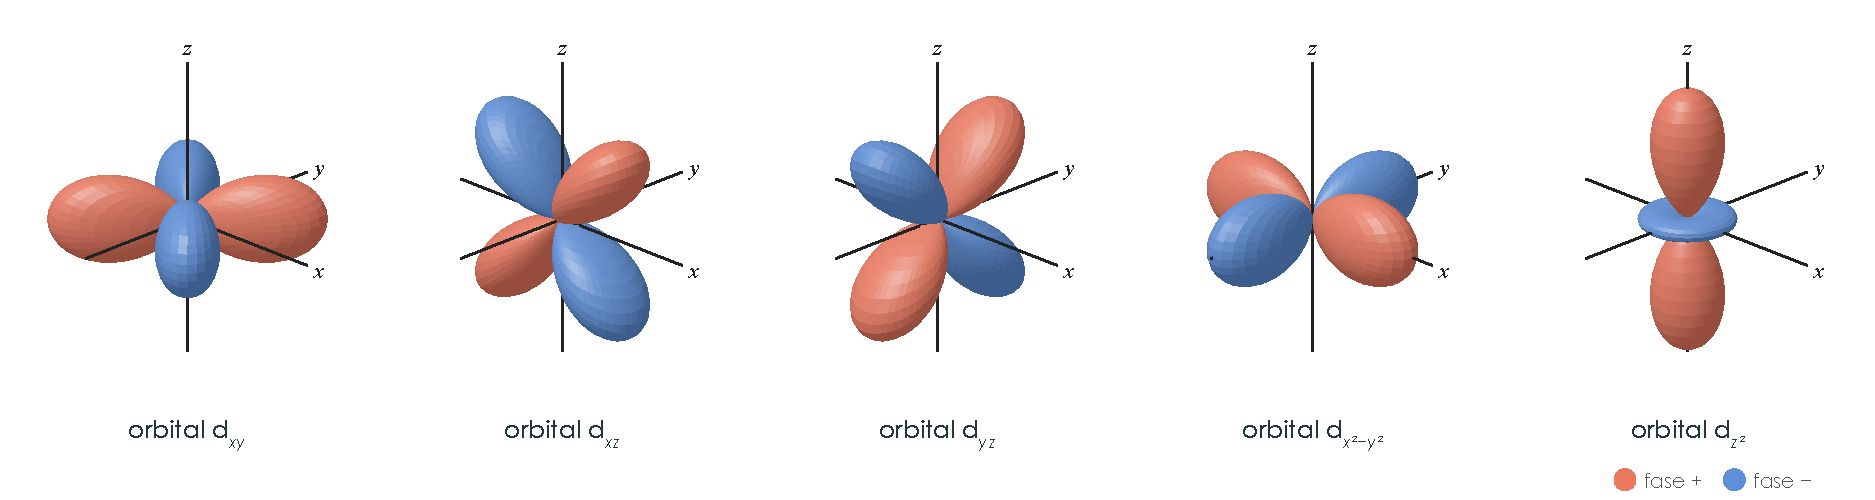
\includegraphics[width=1.0\linewidth]{FigurasSVG/UD1_Estructura_Atomica/pdf/UD1_14_orbitales_d.pdf}
                \caption{Orbitales \(\bm{d}\)}
                %\label{fig:}
            \end{figure}

            \item \textit{l} = 3.
            Orbital \blueremark{f} (fundamental).
            Los tenemos cuando $n\geq 4$.
            Tienen un aspecto multilobular.
            Existen 7 tipos de orbitales $f$ (que corresponden $m=-3, m=-2, m=-1, m= 0, m=+1,m=+2, m=+3$).

            \begin{figure}[H]
                \centering
                % [FIGURA ORIGINAL] \includegraphics[scale=0.7]{images/imagesUD1EstructuraAtomica/UD1_Teoria/orbitalesf}
                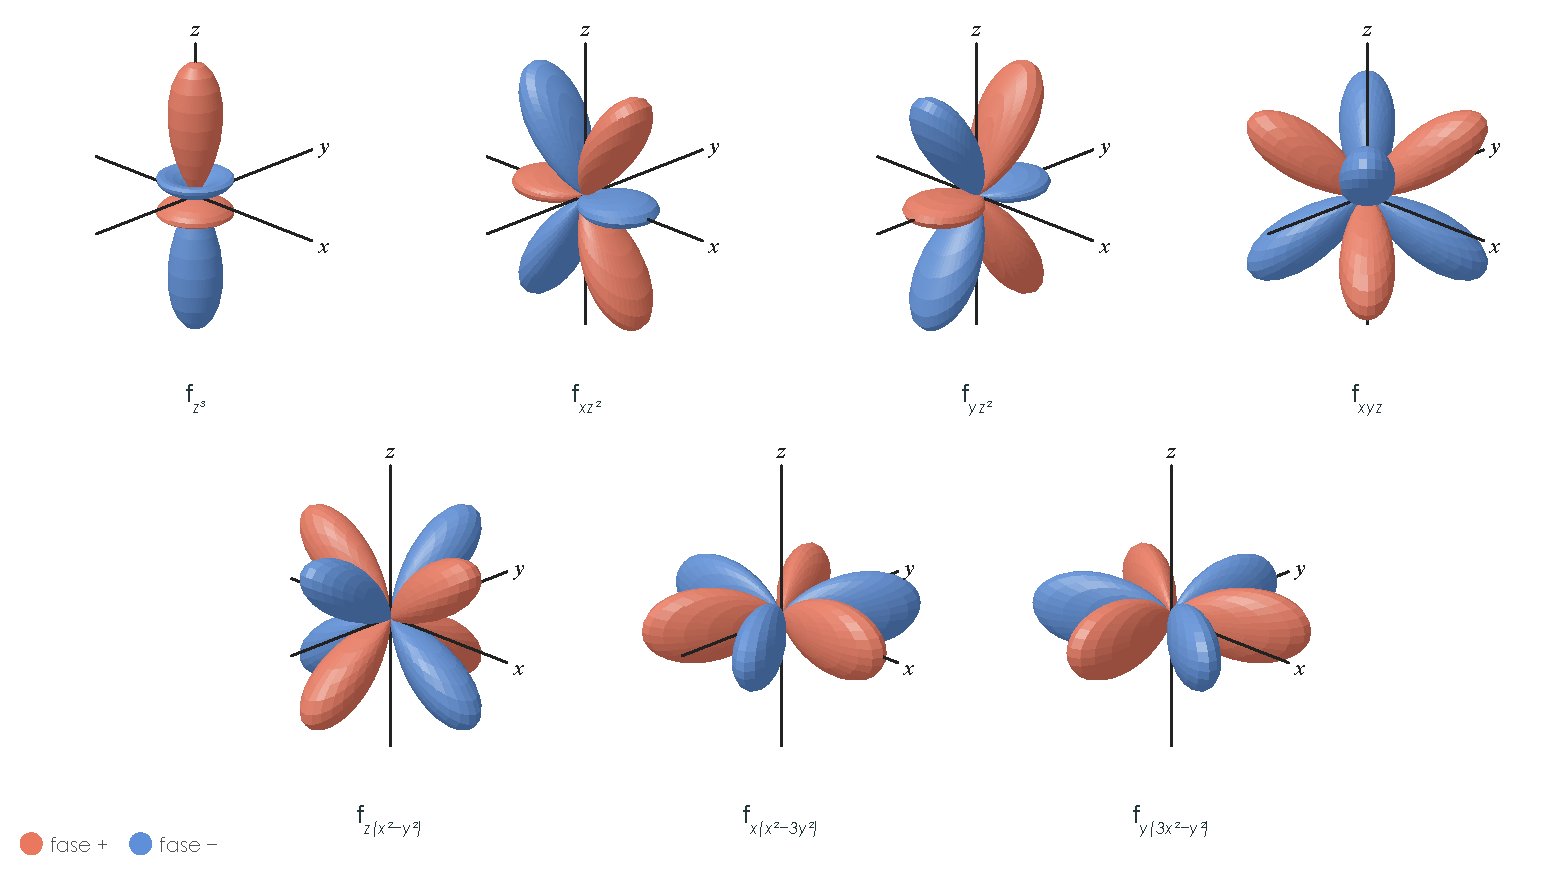
\includegraphics[width=0.9\linewidth]{FigurasSVG/UD1_Estructura_Atomica/pdf/UD1_15_orbitales_f.pdf}
                \caption{Orbitales \(\bm{f}\)}
                %\label{fig:}
            \end{figure}

        \end{enumerate}
        \item \textbf{\textit{m}} es el número cuántico magnético, toma valores desde $-l \dots 0 \dots +l$.
        Determina la orientación espacial del orbital.
        \item \textbf{\textit{s}} es el número cuántico de spin.
        Solo toma los valores $-\frac{1}{2}$ y $+\frac{1}{2}$.
        Determina el giro del electrón sobre sí mismo.
\end{enumerate}
% \begin{figure}
%     \centering
%     \includegraphics[scale=1]{forma_orbitales.png}
%     \caption{Forma de los orbitales atómicos}
%     \label{fig:forma_orbitales}
% \end{figure}

\subsection{Orden energético para los electrones de los átomos}\label{subsec:orden-energetico-para-los-electrones-de-los-atomos}

\subsubsection{Diferentes niveles de energía}

La energía de cada electrón depende de los cuatro números cuánticos.
Según el valor de estos podemos definir, el nivel, el subnivel y el orbital.
\begin{enumerate}[label=\numberballmDarkTeal]
        \item \textbf{Nivel}.
        Los electrones con el mismo número cuántico principal $n$ se dice que forman parte de la misma capa o nivel energético.
        \item \textbf{Subnivel}.
        Cada capa o nivel tiene a su vez subcapas o subniveles.
        Así se dice que en el nivel $n=3$ se encuentran los subniveles $3s\;(l=0)$, $3p\;(l=1)$, $3d\;(l=2)$.
        \item \textbf{Orbital}. Aquellos electrones que tienen los mismos números cuánticos $n$ y $l$ pero diferente $m$ se dice que pertenecen al mismo orbital.
        En cada orbital caben como máximo dos electrones que se diferencian por el número cuántico de spin $s$.
        En cada subnivel $l$ hay $2l+1$ orbitales, con lo que en un nivel $n$ caben $2n^2$ electrones.
\end{enumerate}

Para determinar la energía de cada orbital, se establece que los orbitales con una suma del número cuántico \(n\) y el \(l\) (\(n + l\)) más bajo, tendrán menos energía.
Otra manera de determinarlo es siguiendo el orden de llenado según el diagrama de Moeller.

\subsection{Distribución electrónica}\label{subsec:distribucion-electronica}

La distribución electrónica nos indica como se alojan los diferentes electrones en sus correspondientes orbitales y para ello siguen las siguientes reglas:

\begin{enumerate}[label=\numberballmDarkTeal]
        \item \textbf{Principio de exclusión de Pauli}: Un átomo no puede tener 2 electrones con los mismos 4 números cuánticos.
        En un orbital puede haber como máximo 2 electrones.
        \item \textbf{Principio de mínima energía}: los electrones se colocan en el orbital de menos energía que esté disponible.
        El orden de la energía está determinado por la suma de $n + l$.
        Si dos orbitales tienen el mismo valor de $n+l$, el de menor energía será aquel que tenga menor valor de $n$.

        \item \textbf{Principio de máxima multiplicidad de Hund}: a igualdad de los principios anteriores, la configuración más estable es la que permite el máximo desapareamiento de los electrones.
\end{enumerate}

El orden de llenado también se puede seguir según el diagrama de Moeller.
\begin{figure}[H]
    \centering
    \begin{tikzpicture}[>=stealth, font=\sffamily\LARGE\bfseries]

        % --- Configuración de Colores ---
        \definecolor{mygreen}{RGB}{0, 128, 0}
        \definecolor{myblue}{RGB}{91, 155, 213}

        % --- Dibujado de los Subniveles ---
        % Separación horizontal (2.2) y vertical (1.2) para que las diagonales sean perfectas
        \newcommand{\subnivel}[5]{
            \node (n#3#4) at (#1*2.2, -#2*1.2) {#3\textcolor{mygreen}{\textit{#4}}\textsuperscript{\textcolor{red}{#5}}};
        }

        % Columna s (x=0)
        \foreach \n in {1,...,7} \subnivel{0}{\n}{\n}{s}{2};
        % Columna p (x=1)
        \foreach \n in {2,...,7} \subnivel{1}{\n}{\n}{p}{6};
        % Columna d (x=2)
        \foreach \n in {3,...,7} \subnivel{2}{\n}{\n}{d}{10};
        % Columna f (x=3)
        \foreach \n in {4,...,7} \subnivel{3}{\n}{\n}{f}{14};

        % --- Dibujado de las Flechas Diagonales ---
        % Estilo: pasan por el centro, color azul, y se extienden 0.8cm hacia atrás y 1cm hacia adelante
        \tikzset{flecha/.style={myblue, very thick, *->, shorten <=-0.8cm, shorten >=-1cm}}

        % Para flechas que cruzan varios nodos (del centro del primero al centro del último)
        \draw[flecha] ($(n2p.center)+(1.5,0.7)$) -- (n3s.center);
        \draw[flecha] ($(n3p.center)+(1.5,0.7)$) -- (n4s.center);
        \draw[flecha] ($(n3d.center)+(1.5,0.7)$) -- (n5s.center);
        \draw[flecha] ($(n4d.center)+(1.5,0.7)$) -- (n6s.center);
        \draw[flecha] ($(n4f.center)+(1.5,0.7)$) -- (n7s.center);
        \draw[flecha] ($(n5f.center)+(1.5,0.7)$) -- (n7p.center);
        \draw[flecha] ($(n6f.center)+(1.5,0.7)$) -- (n7d.center);

        % Para las flechas de un solo nodo (1s, 2s y 7f), definimos una dirección manual
        % para que mantengan el mismo ángulo que las demás.
        \draw[flecha] ($(n1s.center)+(1.5,0.7)$) -- (n1s.center);
        \draw[flecha] ($(n2s.center)+(1.5,0.7)$) -- (n2s.center);
        \draw[flecha] (n7f.center) ++(1.5,0.8) -- (n7f.center);

    \end{tikzpicture}
    \caption{Moeller Diagram}
    \label{fig:diagrama_moeller}
\end{figure}
%\begin{figure}[H]
%    \centering
%    \includegraphics[scale=.5]{images/imagesUD1EstructuraAtomica/UD1_Teoria/diagrama_moeller}
%    \caption{Diagrama de Moeller}
%    \label{fig:diagrama_de_moeller}
%\end{figure}

Según estos principios, si un \el{} se encuentra en su estado fundamental estará, por tanto, en un estado de mínima energía.
Si ese \el{} se encuentra excitado, estará, en consecuencia, en un estado de mayor energía, mientras que si un \el{} se encuentra en un estado prohibido será un estado imposible desde el punto de vista cuántico, incumpliendo el principio de exclusión de Pauli.

\subsubsection{Excepciones al orden de llenado y justificación de los estados de oxidación}

Hay excepciones a las reglas de llenado, como por ejemplo:
\begin{itemize}
    \item \elementsymbol{24}(Z=\atomicnumber{Cr}) \elconf{Cr}
    \item \elementsymbol{29}(Z=\atomicnumber{Cu}) \elconf{Cu}
    \item \elementsymbol{47}(Z=\atomicnumber{Ag}) \elconf{Ag}
    \item \elementsymbol{79}(Z=\atomicnumber{Au}) \elconf{Au}
    \item \elementsymbol{42}(Z=\atomicnumber{Mo}) \elconf{Mo}
\end{itemize}

Estas excepciones se deben a que la configuración más estable es aquella que tenga los subniveles \textbf{llenos} / \textbf{capa cerrada}, es decir, aquellos que tienen como configuración electrónica \(ns^2\; np^6\), a excepción del He (\(1s^2\)), o \textbf{semillenos} / \textbf{semicapa cerrada}, es decir, aquellos que tienen como configuración electrónica \(ns^1, \; np^3, \; nd^5, \; nf^7\).

Los estados de oxidación de los elementos se pueden predecir teniendo en cuenta la configuración electrónica. El elemento perderá o ganará electrones de manera que adquiera la configuración electrónica más estable, siendo esta la de gas noble o bien con capas llenas o semillenas.



    \newpage

    %! Author = Profesor
%! Date = 31/05/2024


\section{Ejercicios, Cuestiones y Ejercicios PAU}

\subsection{Ejercicios}

\begin{exercise}
    Calcula la frecuencia umbral y el trabajo de extracción del metal sodio, expresado en electronvoltios (\unit{\electronvolt}), sabiendo qu al incidir sobre una superficie de dicho metal una radiación electromagnética cuya frecuencia es de \SI{1.18e15}{\hertz}, los electrones son arrancados con una energía cinética máxima de \energia[j]{4.18e-19}.
    Determina la velocidad máxima a la que salen los electrones.

    \begin{solu}
        Partimos de la ecuación del efecto fotoeléctrico donde \(h\ \nu = h\ \nu_0 + E_{c}\).
        Sustituyendo los valores y despejando, tenemos que:
        \begin{gather*}
            \num{6.63e-34}\cdot \num{1.18e15} = \num{6.63e-34}\cdot v_0 + \num{4.18e-19}\\
            v_0 = \dfrac{\num{6.63e-34}\cdot \num{1.18e15} - \num{4.18e-19}}{\num{6.63e-34}} = \SI{5.50e14}{\hertz}
        \end{gather*}
        El trabajo de extracción es:
        \begin{equation*}
            W_{umbral} = h\ \nu_0 =  \num{6.63e-34}\cdot \num{5.50e14} = \energia[j]{3.64e-19}
        \end{equation*}
        Ahora hacemos el cambio de julios a electronvoltios
        \begin{equation*}
            \SI{3.64e-19}{\joule}\cdot \dfrac{\SI{1}{\electronvolt}}{\SI{1.6e-19}{\joule}} = \energia[ev]{2.275}
        \end{equation*}
        Ahora el dato de la energía cinética, nos permite calcular la velocidad máxima de ese electrón según:
        \begin{gather*}
            E_c = \dfrac{1}{2}\ m_e \ v_e^2\separ
            v= \sqrt{\dfrac{2\ E_c}{m_e}} = \sqrt{\dfrac{2\cdot \num{4.18e-19}}{\num{9.1e-31}}} = \velocidad[ms]{9.6e5}
        \end{gather*}
        Para calcular el potencial de frenado (\(\Delta V_{frenado}\)), tenemos que saber que \(W = q_e \ \Delta V_{frenado}\) siendo en este caso \(E_c = W\) quedando la expresión de \(\Delta V_{frenado}\) como:
        \begin{equation*}
            \Delta V_{frenado} = \dfrac{\num{4.18e-19}}{\num{1.6e-19}} = \SI{2.6}{\volt}
        \end{equation*}
    \end{solu}
\end{exercise}

\begin{exercise}
    Sabiendo que el trabajo de extracción del cesio vale \energia[ev]{4.3}, ¿cuál es la frecuencia mínima que debe tener una radiación electromagnética para producir efecto fotoeléctrico sobre una lámina de dicho metal?
    ¿Cuál será la máxima longitud de onda?.
    \begin{solu}
%        \begin{figure}[H]
%            \centering
%            \includegraphics[scale=0.4]{images/imagesUD1EstructuraAtomica/UD1_Problemas/ejerciciogeneral_02}
%            %\caption{}
%            %\label{fig:}
%        \end{figure}
        La frecuencia mínima (frecuencia umbral) es aquella para la que toda la energía del fotón se invierte en el trabajo de extracción, es decir, \(h\ \nu_0 = W_0\). Pasando el trabajo de extracción a julios:
        \begin{equation*}
            W_0 = \SI{4.3}{\electronvolt}\cdot \dfrac{\SI{1.6e-19}{\joule}}{\SI{1}{\electronvolt}} = \energia[j]{6.88e-19}
        \end{equation*}
        Despejando la frecuencia umbral:
        \begin{equation*}
            \nu_0 = \dfrac{W_0}{h} = \dfrac{\num{6.88e-19}}{\num{6.63e-34}} = \SI{1.038e15}{\hertz}
        \end{equation*}
        La longitud de onda máxima capaz de producir efecto fotoeléctrico es la asociada a esa frecuencia umbral:
        \begin{equation*}
            \lambda_{max} = \dfrac{c}{\nu_0} = \dfrac{\num{3e8}}{\num{1.038e15}} = \distancia[nm]{289.1}
        \end{equation*}
    \end{solu}
\end{exercise}
%

\begin{exercise}
    Utilizando la ecuación espectral, comprueba los valores de la longitud de onda, la frecuencia y la energía de los fotones emitidos correspondientes a la serie de Balmer.
    \begin{solu}
%        \begin{figure}[H]
%            \centering
%            \includegraphics[scale=0.4]{images/imagesUD1EstructuraAtomica/UD1_Problemas/ejerciciogeneral_03_a.png}
%            \includegraphics[scale=0.4]{images/imagesUD1EstructuraAtomica/UD1_Problemas/ejerciciogeneral_03_b.png}
%            %\caption{}
%            %\label{fig:}
%        \end{figure}
        La serie de Balmer corresponde a las transiciones electrónicas hacia el nivel \(n=2\). La ecuación espectral (Rydberg) permite calcular la longitud de onda emitida:
        \begin{equation*}
            \dfrac{1}{\lambda} = R_H \left(\dfrac{1}{2^2} - \dfrac{1}{n^2}\right) \qquad \text{con } R_H = \SI{1.097e7}{\per\meter},\ n = 3, 4, 5, \ldots
        \end{equation*}
        Para las tres primeras líneas de la serie:
        \begin{gather*}
            n=3:\quad \dfrac{1}{\lambda} = \num{1.097e7}\left(\dfrac{1}{4}-\dfrac{1}{9}\right) = \SI{1.524e6}{\per\meter} \Rightarrow \lambda = \distancia[nm]{656.3}\separ
            n=4:\quad \dfrac{1}{\lambda} = \num{1.097e7}\left(\dfrac{1}{4}-\dfrac{1}{16}\right) = \SI{2.057e6}{\per\meter} \Rightarrow \lambda = \distancia[nm]{486.2}\separ
            n=5:\quad \dfrac{1}{\lambda} = \num{1.097e7}\left(\dfrac{1}{4}-\dfrac{1}{25}\right) = \SI{2.304e6}{\per\meter} \Rightarrow \lambda = \distancia[nm]{434.1}
        \end{gather*}
        A partir de estas longitudes de onda se obtienen la frecuencia (\(\nu = c/\lambda\)) y la energía del fotón (\(E = h\ \nu\)):
        \begin{gather*}
            n=3:\ \nu = \SI{4.571e14}{\hertz},\ E = \energia[j]{3.031e-19}\separ
            n=4:\ \nu = \SI{6.169e14}{\hertz},\ E = \energia[j]{4.090e-19}\separ
            n=5:\ \nu = \SI{6.911e14}{\hertz},\ E = \energia[j]{4.582e-19}
        \end{gather*}
        Estos valores coinciden con los proporcionados por la teoría, confirmando la validez de la ecuación espectral.
    \end{solu}
\end{exercise}

\begin{exercise}
    Calcula la longitud de la onda asociada a un electrón que se mueve con una velocidad igual a un 1\% de la velocidad de la luz.
    \begin{solu}
        La velocidad del electrón es \(v = 0.01\ c = 0.01\cdot \SI{3e8}{\meter\per\second} = \velocidad[ms]{3e6}\).
        Aplicando la ecuación de de Broglie:
        \begin{equation*}
            \lambda = \dfrac{h}{m_e\ v} = \dfrac{\num{6.63e-34}}{\num{9.1e-31}\cdot \num{3e6}} = \distancia[nm]{0.243}
        \end{equation*}
    \end{solu}
\end{exercise}

\begin{exercise}
    Calcula la longitud de la onda asociada a una pelota de tenis de aproximadamente de \masa[g]{50} y que se mueve a una velocidad de \velocidad[kmh]{200}.
    \begin{solu}
        Pasamos la velocidad a unidades del S.I.: \(v = \SI{200}{\kilo\meter\per\hour} = \velocidad[ms]{55.56}\), y la masa a kilogramos: \(m = \masa[kg]{0.05}\).
        Aplicando la ecuación de de Broglie:
        \begin{equation*}
            \lambda = \dfrac{h}{m\ v} = \dfrac{\num{6.63e-34}}{\num{0.05}\cdot \num{55.56}} = \distancia[m]{2.39e-34}
        \end{equation*}
        Esta longitud de onda es tan extremadamente pequeña, comparada con las dimensiones del propio cuerpo, que resulta indetectable; por ello no se observan fenómenos ondulatorios en los objetos macroscópicos.
    \end{solu}
\end{exercise}

\begin{exercise}
    Si un electrón tiene una onda asociada de \distancia[nm]{500}, ¿con qué velocidad se mueve?
    \begin{solu}
%        \begin{figure}[H]
%            \centering
%            \includegraphics[scale=0.4]{images/imagesUD1EstructuraAtomica/UD1_Problemas/ejerciciogeneral_06.png}
%            %\caption{}
%            %\label{fig:}
%        \end{figure}
        De la ecuación de de Broglie \(\lambda = \dfrac{h}{m_e\ v}\) despejamos la velocidad:
        \begin{equation*}
            v = \dfrac{h}{m_e\ \lambda} = \dfrac{\num{6.63e-34}}{\num{9.1e-31}\cdot \num{500e-9}} = \velocidad[ms]{1.46e3}
        \end{equation*}
    \end{solu}
\end{exercise}

%! De oxford libro nuevo lo de arriba.

\begin{exercise}
    Una radiación de \distancia[nm]{300} que incide sobre una lámina de cinc es capaz de provocar la emisión de electrones con una energía cinética de \energia[j]{9.9e-20}. Determina la frecuencia y energía umbral.
    \datos{} \(h = \SI{6.62e-34}{\joule\s}\)

    \begin{solu}
%        \begin{figure}[H]
%            \centering
%            \includegraphics[scale=0.75]{images/imagesUD1EstructuraAtomica/UD1_Problemas/Estrucura_de_la_materia_01.PNG}
%            %\caption{}
%            %\label{fig:}
%        \end{figure}
        La energía del fotón incidente es:
        \begin{equation*}
            E = \dfrac{h\ c}{\lambda} = \dfrac{\num{6.62e-34}\cdot \num{3e8}}{\num{300e-9}} = \energia[j]{6.62e-19}
        \end{equation*}
        Su frecuencia asociada es \(\nu = c/\lambda = \num{3e8}/\num{300e-9} = \SI{1e15}{\hertz}\).
        Aplicando la ecuación del efecto fotoeléctrico \(E = W_0 + E_c\), obtenemos el trabajo (energía) de extracción:
        \begin{equation*}
            W_0 = E - E_c = \num{6.62e-19} - \num{9.9e-20} = \energia[j]{5.63e-19}
        \end{equation*}
        Y la frecuencia umbral:
        \begin{equation*}
            \nu_0 = \dfrac{W_0}{h} = \dfrac{\num{5.63e-19}}{\num{6.62e-34}} = \SI{8.505e14}{\hertz}
        \end{equation*}
    \end{solu}
\end{exercise}

\begin{exercise}
    Una radiación verde monocromática de longitud de onda de \distancia[nm]{570} incide sobre un átomo de hidrógeno. Calcula la energía de un fotón y de un mol de fotones. Compárala con la de las transiciones electrónicas responsables de la primera y segunda línea del Balmer. \datos{} \(h = \SI{6.62e-34}{\joule\s}\); \(R_H = \SI{2.18e-18}{\joule}\).
    \begin{solu}
%        \begin{figure}[H]
%            \centering
%            \includegraphics[scale=0.75]{images/imagesUD1EstructuraAtomica/UD1_Problemas/Estrucura_de_la_materia_02.PNG}
%        \end{figure}
        La energía de un fotón de dicha radiación es:
        \begin{equation*}
            E = \dfrac{h\ c}{\lambda} = \dfrac{\num{6.62e-34}\cdot \num{3e8}}{\num{570e-9}} = \energia[j]{3.484e-19}
        \end{equation*}
        Para un mol de fotones, multiplicamos por el número de Avogadro:
        \begin{equation*}
            E_{mol} = E\cdot N_A = \num{3.484e-19}\cdot \num{6.022e23} = \SI{2.098e5}{\joule\per\mole} \approx \SI{209.8}{\kilo\joule\per\mole}
        \end{equation*}
        Las energías de las transiciones electrónicas de la serie de Balmer (hacia \(n=2\)) se calculan con \(\Delta E = R_H\left(\dfrac{1}{2^2}-\dfrac{1}{n^2}\right)\):
        \begin{gather*}
            n=3\rightarrow 2:\quad \Delta E = \num{2.18e-18}\left(\dfrac{1}{4}-\dfrac{1}{9}\right) = \energia[j]{3.03e-19}\separ
            n=4\rightarrow 2:\quad \Delta E = \num{2.18e-18}\left(\dfrac{1}{4}-\dfrac{1}{16}\right) = \energia[j]{4.09e-19}
        \end{gather*}
        La energía del fotón verde (\(\SI{3.48e-19}{\joule}\)) se encuentra entre la de la primera y la segunda línea de Balmer, por lo que no coincide exactamente con ninguna de las dos transiciones y, por tanto, no sería absorbida por el átomo de hidrógeno en su estado fundamental para producir esas transiciones concretas.
    \end{solu}
\end{exercise}

\begin{exercise}
    Al someter electrones a una diferencia de potencial de \SI{4e4}{\volt} se consigue acelerarlos hasta alcanzar una velocidad de \velocidad[kmh]{4.32e6}.


    \begin{enumerate}[label=\letraminuscula]
        \item Calcula la longitud de onda de los electrones.
        \item La imagen obtenida, ¿se verá en color? ¿Por qué?
    \end{enumerate}
    \datos{} \(h = \SI{6.62e-34}{\joule\s}\); \(m_e = \masa[kg]{9.1e-34}\).

    \begin{solu}
%        \begin{figure}[H]
%            \centering
%            \includegraphics[scale=0.75]{images/imagesUD1EstructuraAtomica/UD1_Problemas/Estrucura_de_la_materia_03.PNG}
%        \end{figure}
        Pasamos la velocidad a unidades del S.I.: \(v = \SI{4.32e6}{\kilo\meter\per\hour} = \velocidad[ms]{1.2e6}\).
        \begin{enumerate}[label=\letraminuscula]
            \item Aplicando la ecuación de de Broglie:
            \begin{equation*}
                \lambda = \dfrac{h}{m_e\ v} = \dfrac{\num{6.62e-34}}{\num{9.1e-31}\cdot \num{1.2e6}} = \distancia[nm]{0.606}
            \end{equation*}
            \item Esta longitud de onda (\(\approx \SI{0.6}{\nano\meter}\)) corresponde a la región de los rayos X, muy alejada del espectro visible (\SIrange{400}{700}{\nano\meter}). Por tanto, la imagen obtenida (propia de un microscopio electrónico) no se verá en color, ya que los electrones no producen radiación visible: la imagen se recoge en blanco y negro (escala de grises) mediante una pantalla fluorescente o un detector electrónico.
        \end{enumerate}
    \end{solu}
\end{exercise}

\begin{exercise}
    Dados los valores de números cuánticos (4,2,3,-1/2); (3,2,1,1/2); (2,0,-1,1/2) y (1,0,0,1/2).
    \begin{enumerate}[label=\letraminuscula]
        \item Indique cuáles de ellos no están permitidos.
        \item Indique el orbital en el que se encontrarían los electrones definidos por los valores de los números cuánticos permitidos.
    \end{enumerate}
    \begin{solu}
%        \begin{figure}[H]
%            \centering
%            \includegraphics[scale=0.75]{images/imagesUD1EstructuraAtomica/UD1_Problemas/Estrucura_de_la_materia_04.PNG}
%        \end{figure}
        Recordemos las restricciones de los números cuánticos \((n,l,m,s)\): \(l = 0, 1, \ldots, n-1\); \(m = -l, \ldots, 0, \ldots, +l\); \(s = \pm 1/2\).
        \begin{itemize}
            \item \((4,2,3,-1/2)\): con \(l=2\), \(m\) debe estar entre \(-2\) y \(2\); como \(m=3\), \textbf{no está permitido}.
            \item \((3,2,1,1/2)\): \(l=2 \leq n-1=2\) y \(m=1\) está entre \(-2\) y \(2\); \textbf{permitido}. Corresponde a un electrón del orbital \(3d\).
            \item \((2,0,-1,1/2)\): con \(l=0\) el único valor posible de \(m\) es \(0\); como \(m=-1\), \textbf{no está permitido}.
            \item \((1,0,0,1/2)\): \(l=0\leq n-1=0\) y \(m=0\); \textbf{permitido}. Corresponde a un electrón del orbital \(1s\).
        \end{itemize}
    \end{solu}
\end{exercise}

\begin{exercise}
    Dados los siguientes conjuntos de números cuánticos: (2,1,2,+1/2); (3,1,-1,+1/2); (2,2,1,-1/2) y (3,2,- 2,+1/2): a) Expresar el significado de los cuatro números cuánticos; b) Razonar cuáles son permitidos y cuales no.
    c) Explicar cuál de los permitidos se corresponde con un electrón en un orbital d.

    \begin{solu}
        \begin{enumerate}[label=\letraminuscula]
            \item Significado de los números cuánticos:
            \begin{itemize}
                \item \(n\) (principal): indica el nivel de energía y el tamaño del orbital.
                \item \(l\) (secundario o azimutal): indica la forma del orbital (subnivel \(s,p,d,f\)) y toma valores de \(0\) a \(n-1\).
                \item \(m\) (magnético): indica la orientación espacial del orbital y toma valores enteros entre \(-l\) y \(+l\).
                \item \(s\) (de espín): indica el sentido de giro del electrón sobre sí mismo, \(+1/2\) o \(-1/2\).
            \end{itemize}
            \item Análisis de cada conjunto:
            \begin{itemize}
                \item \((2,1,2,+1/2)\): con \(l=1\), \(m\) debe estar entre \(-1\) y \(1\); como \(m=2\), \textbf{no permitido}.
                \item \((3,1,-1,+1/2)\): \(l=1\leq n-1=2\) y \(m=-1\) está en el rango correcto; \textbf{permitido} (orbital \(3p\)).
                \item \((2,2,1,-1/2)\): con \(n=2\), \(l\) solo puede valer \(0\) o \(1\); como \(l=2\), \textbf{no permitido}.
                \item \((3,2,-2,+1/2)\): \(l=2\leq n-1=2\) y \(m=-2\) está entre \(-2\) y \(2\); \textbf{permitido} (orbital \(3d\)).
            \end{itemize}
            \item El conjunto permitido que corresponde a un electrón en un orbital \(d\) es \((3,2,-2,+1/2)\), ya que \(l=2\) define el subnivel \(d\).
        \end{enumerate}
    \end{solu}
\end{exercise}

\begin{exercise}
    Escribe la configuración electrónica para los siguientes elementos con los siguientes números atómicos: Z = 26, Z = 50, Z = 19.
    \begin{solu}
        Siguiendo el orden de llenado de orbitales (principio de Aufbau):
        \begin{itemize}
            \item \(Z=26\) (Fe): \(1s^2\ 2s^2\ 2p^6\ 3s^2\ 3p^6\ 4s^2\ 3d^6\)
            \item \(Z=50\) (Sn): \(1s^2\ 2s^2\ 2p^6\ 3s^2\ 3p^6\ 4s^2\ 3d^{10}\ 4p^6\ 5s^2\ 4d^{10}\ 5p^2\)
            \item \(Z=19\) (K): \(1s^2\ 2s^2\ 2p^6\ 3s^2\ 3p^6\ 4s^1\)
        \end{itemize}
    \end{solu}
\end{exercise}

\begin{exercise}
    Escribe la configuración electrónica para \ch{Cr}, \ch{Cu} y \ch{Ag}.
    Compara los resultados con las configuraciones electrónicas de los apuntes.
    \begin{solu}
        Estos tres elementos son excepciones al principio de Aufbau, ya que adquieren una mayor estabilidad con subniveles \(d\) semillenos o completamente llenos:
        \begin{itemize}
            \item \(\ch{Cr}\) (\(Z=24\)): configuración esperada \(4s^2\ 3d^4\); configuración real \([\ch{Ar}]\ 4s^1\ 3d^5\), más estable por tener el subnivel \(3d\) semilleno.
            \item \(\ch{Cu}\) (\(Z=29\)): configuración esperada \(4s^2\ 3d^9\); configuración real \([\ch{Ar}]\ 4s^1\ 3d^{10}\), más estable por tener el subnivel \(3d\) completamente lleno.
            \item \(\ch{Ag}\) (\(Z=47\)): configuración esperada \(5s^2\ 4d^9\); configuración real \([\ch{Kr}]\ 5s^1\ 4d^{10}\), más estable por tener el subnivel \(4d\) completamente lleno.
        \end{itemize}
        En los tres casos, la promoción de un electrón \(s\) al subnivel \(d\) inmediatamente inferior proporciona una configuración de menor energía (mayor estabilidad) que la predicha por el orden estricto de llenado.
    \end{solu}
\end{exercise}

\subsection{Cuestiones}

\begin{question}
    Indica qué diferencia existe entre energía e intensidad de la radiación.
    \begin{solu}
        La energía de una radiación es la energía de cada uno de sus
        fotones y se relaciona con la frecuencia de la radiación; tiene
        que ver con el efecto cualitativo que puede tener la radiación.
        La intensidad de una radiación depende del número de fotones
        y tiene que ver con el efecto cuantitativo de la radiación.
    \end{solu}

\end{question}

\begin{question}
    ¿Por qué la radiación ilumina una placa metálica (y no provoca en ella efecto fotoeléctrico) seguirá sin provocarlo aunque aumentemos mucho su intensidad?
    \begin{solu}
        Si la radiación no provoca el efecto fotoeléctrico es porque
        sus fotones no tienen energía suficiente para arrancar los
        electrones de la placa.
        Al aumentar la intensidad de la radiación
        solo crece el número de fotones, pero no cambia su
        energía.
    \end{solu}
\end{question}

\begin{question}
    Indica la diferencia entre órbita y orbital.
    \begin{solu}
        De acuerdo con la teoría de Bohr, órbita es la curva que describe
        el electrón cuando gira alrededor de su núcleo.
        Por
        su parte, el orbital es un concepto mecanocuántico que se
        refiere a la región del espacio donde existe una probabilidad
        de encontrar un electrón superior al 90 \%.
    \end{solu}
\end{question}

\begin{question}
    Teniendo en cuenta el modelo atómico de Bohr, indica si un electrón que se encuentra en la órbita de \(n = 4\) se mueve más rápido o más lento que uno que se halle en la órbita de \(n = 2\).

    \begin{solu}
        La velocidad del electrón es directamente
        proporcional al número cuántico principal e inversamente
        proporcional al radio de la órbita.
        Combinando ambos factores
        resulta que la velocidad es inversamente proporcional al
        número cuántico n, esto es, cuanto mayor es dicho número,
        menor es la velocidad del electrón.
    \end{solu}
\end{question}

\begin{question}
    Razona sobre la veracidad de la siguiente afirmación:

    «Un electrón que se encuentra en el nivel 4 de energía está a doble distancia del núcleo que uno que se halla en el nivel 2 de energía».
    \begin{solu}
        La distancia al núcleo viene determinada por el radio de la órbita, y esta depende de \(n^2\)  (\(r = a\ n^2\) ). El electrón que está en la órbita de \(n = 4\)  está a una distancia del núcleo \(r = 16a\) ,      mucho mayor que el doble de aquella a la que está en \(n = 2\) ,
        es decir, \(r = 4a\) .
    \end{solu}
\end{question}

\begin{question}
    Explica si la diferencia de energía entre los niveles 7 y 8 de un átomo es igual, mayor o menor que la diferencia de energía entre los niveles 2 y 3.
    \begin{solu}
        Cuanto más alejados estén los electrones del núcleo, menor será la diferencia de energía entre niveles consecutivos.
        Aplicando la fórmula:
%        \begin{figure}[H]
%            \centering
%            \includegraphics[scale=1]{images/imagesUD1EstructuraAtomica/UD1_Problemas/cuestion7}
%            %\caption{}
%            %\label{fig:}
%        \end{figure}

        \begin{align*}
            \Delta E_{7-8} &= -b\,\frac{1}{8^2} - \left(-b\,\frac{1}{7^2}\right) = b\left(\frac{1}{7^2} - \frac{1}{8^2}\right) = \num{4.78e-3}\,b \\
            \Delta E_{2-3} &= -b\,\frac{1}{3^2} - \left(-b\,\frac{1}{2^2}\right) = b\left(\frac{1}{2^2} - \frac{1}{3^2}\right) = \num{0.14}\,b
        \end{align*}
    \end{solu}
\end{question}

\begin{question}
    ¿Qué significa que un electrón se encuentra en su estado fundamental, en un estado excitado o en un estado prohibido?
    \begin{solu}
        Estado fundamental es el estado de menor energía para el electrón.
        Estado excitado es cualquier estado posible para el electrón con una energía mayor que la del estado fundamental. El electrón llega a ese estado cuando se le comunica energía y,
        en cuanto cesa la excitación, vuelve al estado fundamental.
        Estado prohibido es un estado cuánticamente imposible para
        el electrón, por ejemplo un estado en el que se incumple el
        principio de exclusión de Pauli.
    \end{solu}
\end{question}

\begin{question}
    Explica la siguiente frase: «El espectro de absorción de una sustancia es el complementario del de emisión».
    \begin{solu}
        El espectro de absorción es el análisis de las radiaciones que
        absorben los electrones de un átomo y que le permiten pasar
        de un nivel de energía a otro más exterior (estados excitados
        del electrón). Cuando el electrón deja de estar excitado, hace
        el tránsito inverso, lo que se recoge en el espectro de emisión.
        Por eso ambos espectros son complementarios.
    \end{solu}
\end{question}

\begin{question}
    ¿Por qué el espectro de un elemento químico es distinto del de cualquier otro y sirve para identificarlo?

    \begin{solu}
        El espectro mide diferencias de energía entre niveles de un electrón.
        La energía del electrón en un
        nivel depende de la carga del núcleo del átomo al que pertenezca,
        y esta es distinta para cada elemento químico, ya que depende de su número atómico.
    \end{solu}
\end{question}

\begin{question}
    Utilizando la fórmula de Rydberg, idea un método para medir la energía de ionización de un átomo.

    \begin{solu}
        Se tendrá que medir la energía correspondiente al tránsito entre el nivel en que se encuentra el electrón en la capa de valencia de un átomo y el nivel de \(n = \infty\).
%        \begin{figure}[H]
%            \centering
%            \includegraphics[scale=1]{images/imagesUD1EstructuraAtomica/UD1_Problemas/cuestion11}
%            %\caption{}
%            %\label{fig:}
%        \end{figure}

        \[
            \frac{1}{\lambda} = R\left(\frac{1}{n_1^2} - \frac{1}{\infty}\right); \qquad c = \lambda\,\nu; \qquad E = h\,\frac{c}{\lambda}
        \]
    \end{solu}
\end{question}

\begin{question}
    Explica por qué no se observan los fenómenos ondulatorios en el mundo macroscópico.
    ¿Sería posible observar la onda asociada a una pelota de tenis que va de un
    lado a otro de la cancha?

    \begin{solu}
        La longitud de onda asociada a un cuerpo que se mueve se calcula por la fórmula de Louis de Broglie:

        \begin{equation*}
            \lambda = \dfrac{h}{m\ v}
        \end{equation*}

        Como el valor de h es del orden de \num{e-34} , los cuerpos macroscópicos,
        cuya masa es del orden de 1 kg y cuya velocidad
        es del orden de 1 m/s, tendrán una longitud de onda asociada
        tan pequeña que no se podrán observar fenómenos
        ondulatorios. Para que se observara difracción, la radiación
        tendría que atravesar rendijas de un tamaño comparable a
        su longitud de onda. Las rendijas más pequeñas son las
        que corresponden a la distancia interatómica, que se puede
        obtener cuando una radiación atraviesa una red metálica.
        Solo partículas comparables a las partículas atómicas - como
        el electrón - presentan fenómenos ondulatorios observables.
    \end{solu}

\end{question}

\begin{question}
    Razona si se pueden determinar, con total precisión y a la vez, la posición y la cantidad de movimiento de una pelota de tenis. Extiende tu razonamiento para ver si es posible determinar, con la misma precisión, esos valores
    en el caso de un electrón. ¿Cabe esperar que el avance tecnológico permita en el futuro determinar dichas magnitudes sin ningún tipo de error?

    \begin{solu}
        El principio de incertidumbre permite determinar el grado de error con que se pueden conocer, a la vez, la posición y el estado de movimiento de los cuerpos. El límite inferior de esta incertidumbre es \(h/2\pi\).

        En los cuerpos macroscópicos, cuya masa es del orden de 1 kg y cuya velocidad es del orden de 1 m/s, la incertidumbre es inapreciable, por lo que podríamos establecer con total precisión y simultáneamente la posición y la cantidad de movimiento de la pelota de tenis.
        En el caso de un electrón, por su parte, tanto su masa como las dimensiones de sus
        órbitas entran en los órdenes de magnitud de h y, por tanto, habrá un error inevitable en la determinación de su posición y su estado de movimiento, que no se podrá superar con
        ningún avance tecnológico.
    \end{solu}
\end{question}

\begin{question}
    Utiliza el principio de dualidad onda-corpúsculo y el concepto de órbita estacionaria para justificar el segundo
    postulado de Bohr.
    \begin{solu}
        Según la dualidad onda-corpúsculo, a todo electrón en movimiento se le puede asociar una onda cuya longitud viene dada por la ecuación de de Broglie: \(\lambda = h/(m\ v)\).
        Para que una órbita sea estacionaria (que el electrón no pierda energía al girar), la onda asociada al electrón debe ser una onda estacionaria, es decir, debe encajar un número entero de veces en el perímetro de la órbita:
        \begin{equation*}
            2\pi\ r = n\ \lambda \qquad (n = 1, 2, 3, \ldots)
        \end{equation*}
        Sustituyendo \(\lambda\) por la expresión de de Broglie:
        \begin{gather*}
            2\pi\ r = n\ \dfrac{h}{m\ v}\separ
            m\ v\ r = n\ \dfrac{h}{2\pi}
        \end{gather*}
        Esta última expresión es precisamente el segundo postulado de Bohr: el momento angular del electrón (\(m\ v\ r\)) solo puede tomar valores múltiplos enteros de \(h/2\pi\), es decir, está cuantizado.
    \end{solu}
\end{question}

\begin{question}
    ¿Cuántos electrones caben en los orbitales del nivel \(n = 3\) ? ¿Y en los del nivel \(n = 4\)?
    \begin{solu}
        En los orbitales de \( n = 3\) caben 18 electrones y en los de \(n = 4\), 32 electrones.
    \end{solu}
\end{question}

\subsection{Ejercicios PAU}\label{subsec:ejercicios-evau-clm}

\begin{exerciseEVAU}
    Responda a las siguientes cuestiones:
    \begin{enumerate}[label=\letraminuscula]
        \item Explique cuáles de los siguientes grupos de números cuánticos son imposibles para un
electrón en un átomo: (4, 2, 0, +1/2) (3, 3, 2,-1/2) (2,0,1,+1/2) (3,1,1,-1/2).
        \item Explique los orbitales donde se sitúan los electrones que corresponden con los grupos de números cuánticos anteriores que están permitidos.
        \item Justifique cuál de dichos orbitales tiene mayor energía.
    \end{enumerate}
    \begin{solu}
        \begin{enumerate}[label=\letraminuscula]
            \item Recordando que \(l\) va de \(0\) a \(n-1\) y \(m\) de \(-l\) a \(+l\):
            \begin{itemize}
                \item \((4,2,0,+1/2)\): \(l=2\leq 3\) y \(m=0\in[-2,2]\); \textbf{permitido}.
                \item \((3,3,2,-1/2)\): con \(n=3\), \(l\) solo puede ser \(0,1,2\); como \(l=3\), \textbf{no permitido}.
                \item \((2,0,1,+1/2)\): con \(l=0\), \(m\) solo puede ser \(0\); como \(m=1\), \textbf{no permitido}.
                \item \((3,1,1,-1/2)\): \(l=1\leq 2\) y \(m=1\in[-1,1]\); \textbf{permitido}.
            \end{itemize}
            \item El conjunto \((4,2,0,+1/2)\) corresponde a un electrón del orbital \(4d\). El conjunto \((3,1,1,-1/2)\) corresponde a un electrón del orbital \(3p\).
            \item El orbital \(4d\) tiene mayor energía que el \(3p\), ya que al aumentar el número cuántico principal \(n\) aumenta la energía del electrón (el orbital está más alejado del núcleo y menos ligado a él).
        \end{enumerate}
    \end{solu}
\end{exerciseEVAU}


\begin{exerciseEVAU}
    \textbf{Año 2022}.
    Señale cuáles de las siguientes combinaciones de números cuánticos de un electrón en un átomo no son correctas e indique en su caso la razón.
    \begin{center}
        (2,1,-1,1/2) (3,2,-2,0) (2,2,1,1/2) (3,0,0,-1/2)
    \end{center}
    \begin{solu}
        \begin{itemize}
            \item \((2,1,-1,1/2)\): \(l=1\leq n-1=1\), \(m=-1\in[-1,1]\), \(s=1/2\); \textbf{correcta}.
            \item \((3,2,-2,0)\): el número de espín solo puede valer \(+1/2\) o \(-1/2\); como \(s=0\), \textbf{incorrecta}.
            \item \((2,2,1,1/2)\): con \(n=2\), \(l\) solo puede ser \(0\) o \(1\); como \(l=2\), \textbf{incorrecta}.
            \item \((3,0,0,-1/2)\): \(l=0\leq n-1=2\) y \(m=0\); \textbf{correcta}.
        \end{itemize}
    \end{solu}
\end{exerciseEVAU}

\begin{exerciseEVAU}
    \textbf{Año 2022}.
    Señale cuáles de las siguientes combinaciones de números cuánticos no son correctas e indique la razón: a) (4, 3, 2, 1); b) (1, 0, -1, -1/2); c) (4, 0, 1,1/2); d) (3, 2, -2, 1/2)
    \begin{solu}
%        \begin{figure}[H]
%            \centering
%            \includegraphics[scale=.6]{images/imagesUD1EstructuraAtomica/UD1_Problemas/evauclm12.png}
%        \end{figure}
        \begin{itemize}
            \item a) \((4,3,2,1)\): el número de espín solo puede ser \(\pm 1/2\); como \(s=1\), \textbf{incorrecta}.
            \item b) \((1,0,-1,-1/2)\): con \(l=0\), \(m\) solo puede ser \(0\); como \(m=-1\), \textbf{incorrecta}.
            \item c) \((4,0,1,1/2)\): con \(l=0\), \(m\) solo puede ser \(0\); como \(m=1\), \textbf{incorrecta}.
            \item d) \((3,2,-2,1/2)\): \(l=2\leq n-1=2\), \(m=-2\in[-2,2]\), \(s=1/2\); \textbf{correcta}.
        \end{itemize}
    \end{solu}
\end{exerciseEVAU}

\begin{exerciseEVAU}
    \textbf{Año 2022}.
    Copie y complete en el cuadernillo (no en este enunciado) los huecos de la siguiente tabla correspondientes a átomos
    neutros.
    \begin{table}[H]
        \centering
        \vspace{-5pt}
        % aumenta la altura de las filas
        \renewcommand{\arraystretch}{2}
        % --- tabla antigua ---
        % \begin{tabular}{|c|p{1.5cm}|p{1.5cm}|p{1.5cm}|p{1.5cm}|}
            % \cline{2-5}
            % \multicolumn{1}{c|}{\textbf{}} & \centering \textbf{\isotope{89,Sr}} & \centering  \textbf{\isotope{127,Sn}} & \textbf{} &   \\
            % \hline
            % Electrones                     &                                     &                                     &              & 6 \\
            % \hline
            % Neutrones                      &                                     &                                     &              & 6 \\
            % \hline
            % A                              &                                     &                                     & \centering 5 &   \\
            % \hline
            % Z                              &                                     &                                     & \centering 2 &   \\
            % \hline
        % \end{tabular}
        % --- tabla nueva ---
        \begin{tabular}{@{}cp{1.5cm}p{1.5cm}p{1.5cm}p{1.5cm}@{}}
            \toprule
            \multicolumn{1}{c|}{\textbf{}} & \centering \textbf{\isotope{89,Sr}} & \centering  \textbf{\isotope{127,Sn}} & \textbf{} &  \\
            \midrule
            Electrones &  &  &  & 6 \\[3pt]
            Neutrones &  &  &  & 6 \\[3pt]
            A &  &  & \centering 5 &  \\[3pt]
            Z &  &  & \centering 2 &  \\
            \bottomrule
        \end{tabular}
        \label{tab:}
    \end{table}

    \begin{solu}
%        \begin{figure}[H]
%            \centering
%            \includegraphics[scale=.6]{images/imagesUD1EstructuraAtomica/UD1_Problemas/evauclm12nuevo.png}
%        \end{figure}
        Para átomos neutros el número de electrones coincide con el número atómico \(Z\), y el número de neutrones es \(A - Z\).
        \begin{itemize}
            \item \(\isotope{89,Sr}\): \(Z=38\), \(A=89 \Rightarrow\) neutrones \(=89-38=51\); electrones \(=38\).
            \item \(\isotope{127,Sn}\): \(Z=50\), \(A=127 \Rightarrow\) neutrones \(=127-50=77\); electrones \(=50\).
            \item Tercera columna (\(A=5\), \(Z=2\), es decir \(\isotope{5,He}\)): neutrones \(=5-2=3\); electrones \(=Z=2\).
            \item Cuarta columna (electrones \(=6\), neutrones \(=6\)): al ser neutro, \(Z=6\) (carbono) y \(A=Z+\text{neutrones}=6+6=12\), es decir \(\isotope{12,C}\).
        \end{itemize}
    \end{solu}
\end{exerciseEVAU}

\begin{exerciseEVAU}
    \textbf{Año 2023}.
    Para un átomo en su estado fundamental, razone la veracidad o falsedad de las siguientes
    afirmaciones:
    \begin{enumerate}[label=\letraminuscula]
\item El número máximo de electrones con número cuántico n = 3 es 6.
\item En un orbital 2p solo puede haber 2 electrones.
\item Si en los orbitales 3d se sitúan 6 electrones, no habrá ninguno desapareado.
\item Para un orbital 4d, n = 4 y l = 2.
    \end{enumerate}
    \begin{solu}
%        \begin{figure}[H]
%            \centering
%            \includegraphics[scale=.7]{images/imagesUD1EstructuraAtomica/UD1_Problemas/evauclm13.png}
%        \end{figure}
        \begin{enumerate}[label=\letraminuscula]
            \item \textbf{Falsa}. El número máximo de electrones con \(n=3\) es \(2n^2 = 2\cdot 3^2 = 18\), no 6.
            \item \textbf{Verdadera}. Cada orbital, por el principio de exclusión de Pauli, puede alojar como máximo 2 electrones con espines opuestos.
            \item \textbf{Falsa}. El subnivel \(3d\) tiene 5 orbitales. Según la regla de Hund, los 6 electrones se distribuyen ocupando primero cada orbital de forma individual (5 electrones desapareados) y el sexto electrón se aparea en uno de ellos, quedando 4 electrones desapareados (no ninguno).
            \item \textbf{Verdadera}. En un orbital \(4d\), el número cuántico principal es \(n=4\) y, al tratarse de un orbital \(d\), el número cuántico secundario es \(l=2\).
        \end{enumerate}
    \end{solu}
\end{exerciseEVAU}

\begin{exerciseEVAU}
    \textbf{Año 2021}.
    Señale cuáles de las siguientes combinaciones de números cuánticos no son correctas e indique la razón: a) (3, 2, 0, +1/2); b) (1, 1, 0, -1/2); c) (2, 0, 1, + 1/2); d) (2, 1, -1, 0); e) (4, 2, -1, -1/2)
    \begin{solu}
%        \begin{figure}[H]
%            \centering
%            \includegraphics[scale=.5]{images/imagesUD1EstructuraAtomica/UD1_Problemas/evauclm17.png}
%        \end{figure}
        \begin{itemize}
            \item a) \((3,2,0,+1/2)\): \(l=2\leq n-1=2\), \(m=0\in[-2,2]\); \textbf{correcta}.
            \item b) \((1,1,0,-1/2)\): con \(n=1\), \(l\) solo puede ser \(0\); como \(l=1\), \textbf{incorrecta}.
            \item c) \((2,0,1,+1/2)\): con \(l=0\), \(m\) solo puede ser \(0\); como \(m=1\), \textbf{incorrecta}.
            \item d) \((2,1,-1,0)\): el espín solo puede valer \(\pm 1/2\); como \(s=0\), \textbf{incorrecta}.
            \item e) \((4,2,-1,-1/2)\): \(l=2\leq n-1=3\), \(m=-1\in[-2,2]\); \textbf{correcta}.
        \end{itemize}
    \end{solu}
\end{exerciseEVAU}

\begin{exerciseEVAU}
    \textbf{Año 2021}.
    Justifique, razonadamente, si es verdadera o falsa la siguiente propuesta:
    \begin{enumerate}[label=\letraminuscula]
        \item Todos los isótopos de un mismo elemento químico tienen el mismo número de neutrones y de protones.
        \item Complete los huecos de la siguiente tabla correspondientes a átomos neutros.
    \end{enumerate}
    \begin{table}[H]
        \centering
        \vspace{-5pt}
        % aumenta la altura de las filas
        \renewcommand{\arraystretch}{2}
        % --- tabla antigua ---
        % \begin{tabular}{|c|p{1.5cm}|p{1.5cm}|p{1.5cm}|p{1.5cm}|}
            % \cline{2-5}
            % \multicolumn{1}{c|}{\textbf{}} & \centering \textbf{\isotope{39,K}} & \centering  \textbf{\isotope{14,N}} & \textbf{} &   \\
            % \hline
            % Protones                     &                                     &                                     &  \centering   15         &  \\
            % \hline
            % Neutrones                      &                                     &                                     &              & 8 \\
            % \hline
            % Electrones                              &                                     &                                     & \centering  &  6 \\
            % \hline
            % A                              &                                     &                                     & \centering 31 &   \\
            % \hline
        % \end{tabular}
        % --- tabla nueva ---
        \begin{tabular}{@{}cp{1.5cm}p{1.5cm}p{1.5cm}p{1.5cm}@{}}
            \toprule
            \multicolumn{1}{c|}{\textbf{}} & \centering \textbf{\isotope{39,K}} & \centering  \textbf{\isotope{14,N}} & \textbf{} &  \\
            \midrule
            Protones &  &  & \centering   15 &  \\[3pt]
            Neutrones &  &  &  & 8 \\[3pt]
            Electrones &  &  & \centering & 6 \\[3pt]
            A &  &  & \centering 31 &  \\
            \bottomrule
        \end{tabular}
        \label{tab:}
    \end{table}
%    \begin{table}[H]
%        \centering
%        \vspace{-5pt}
%        % aumenta la altura de las filas
%        \renewcommand{\arraystretch}{2}
%        \begin{tabular}{|c|p{1.5cm}|p{1.5cm}|p{1.5cm}|p{1.5cm}|}
%            \cline{2-5}
%            \multicolumn{1}{c|}{\textbf{}} & \centering \textbf{\isotope{39,K}} & \centering  \textbf{\isotope{14,N}} & \textbf{} &   \\
%            \hline
%            Electrones                     &                                    &                                   & \centering 15 &              \\
%            \hline
%            Neutrones                      &                                    &                                   &               & \centering 8 \\
%            \hline
%            A                              &                                    &                                   &               & \centering 6 \\
%            \hline
%            Z                              &                                    &                                   & \centering 31 &              \\
%            \hline
%        \end{tabular}
%        \label{tab:}
%    \end{table}
%    \begin{table}[H]
%        \centering
%        \begin{tblr}{
%            colspec = {Q[c,m]|Q[c,m]|Q[c,m]|Q[c,m]|Q[c,m]},
%            row{1} = {bg=mybluecolour, fg = white, font=\sffamily},
%            vlines = {1}{white},
%        }
%            Símbolo    & \isotope{39,K} & \isotope{14,N} &    &   \\
%            \hline
%            Protones   &                &                & 15 &   \\
%            \hline
%            Neutrones  &                &                &    & 8 \\
%            \hline
%            Electrones &                &                &    & 6 \\
%            \hline
%            \(A\)      &                &                & 31 &   \\
%            \hline
%        \end{tblr}
%    \end{table}
    \begin{solu}
%        \begin{figure}[H]
%            \centering
%            \includegraphics[scale=.5]{images/imagesUD1EstructuraAtomica/UD1_Problemas/evauclm18.png}
%        \end{figure}
        \begin{enumerate}[label=\letraminuscula]
            \item \textbf{Falsa}. Los isótopos de un mismo elemento tienen el mismo número de protones (mismo \(Z\)), pero distinto número de neutrones (y por tanto distinta masa atómica \(A\)).
            \item Para átomos neutros, protones = electrones = \(Z\), y neutrones \(= A - Z\):
            \begin{itemize}
                \item \(\isotope{39,K}\): \(Z=19\), \(A=39 \Rightarrow\) protones \(=19\), electrones \(=19\), neutrones \(=39-19=20\).
                \item \(\isotope{14,N}\): \(Z=7\), \(A=14 \Rightarrow\) protones \(=7\), electrones \(=7\), neutrones \(=14-7=7\).
                \item Tercera columna (protones \(=15\), \(A=31\), fósforo): neutrones \(=31-15=16\); electrones \(=15\).
                \item Cuarta columna (neutrones \(=8\), electrones \(=6\)): al ser neutro, \(Z=6\) (carbono) y \(A=Z+\text{neutrones}=6+8=14\); protones \(=6\).
            \end{itemize}
        \end{enumerate}
    \end{solu}
\end{exerciseEVAU}

\begin{exerciseEVAU}
    \textbf{2021}.
    Explique el significado físico de cada uno de los números cuánticos. b) Escriba dos combinaciones posibles de números cuánticos para los electrones de valencia del átomo con Z = 20.
    \begin{solu}
%        \begin{figure}[H]
%            \centering
%            \includegraphics[scale=0.5]{images/imagesUD1EstructuraAtomica/UD1_Problemas/evauclm19.png}
%        \end{figure}
        Significado físico de los números cuánticos:
        \begin{itemize}
            \item \(n\) (principal): determina el nivel de energía del electrón y el tamaño del orbital.
            \item \(l\) (secundario o azimutal): determina la forma del orbital (subnivel \(s, p, d, f\)), con valores de \(0\) a \(n-1\).
            \item \(m\) (magnético): determina la orientación espacial del orbital, con valores enteros entre \(-l\) y \(+l\).
            \item \(s\) (de espín): indica el sentido del giro del electrón sobre sí mismo, \(+1/2\) o \(-1/2\).
        \end{itemize}
        El átomo con \(Z=20\) es el calcio, cuya configuración electrónica termina en \(4s^2\); sus electrones de valencia se encuentran, por tanto, en el orbital \(4s\) (\(n=4\), \(l=0\), \(m=0\)). Dos combinaciones posibles de números cuánticos para estos electrones son:
        \begin{center}
            \((4,0,0,+1/2)\) \qquad y \qquad \((4,0,0,-1/2)\)
        \end{center}
    \end{solu}
\end{exerciseEVAU}

\


    \chapter{Tabla Periódica}

    \spacing{1.3}
\renewcommand{\tablename}{Tabla}


%\section{Organización de la Tabla Periódica (TP) de los elementos}\label{sec:organizacion-de-la-tabla-periodica-(tp)-de-los-elementos}
%
%A partir del siglo XIX, la clasificación de los elementos químicos conocidos hasta el momento se convirtió en una necesidad.
%
%\subsection{Primeros intentos de clasificación}\label{subsec:primeros-intentos-de-clasificacion}
%
%\begin{enumerate}
%    \item \textbf{Distinción entre metales y no metales}.
%    \item \textbf{Triadas de Döbereiner}.
%    Consistía en agrupar los elementos de tres en tres de tal forma que la masa atómica del segundo constituyese aproximadamente la media de las masas atómicas de los otros dos, además, las propiedades químicas del elemento central eran intermedias con respecto a las de los otros dos.
%    \item \textbf{Octavas de Newlands}.
%    Disponía los elementos químicos por orden creciente de su masa atómica, resultaba que cada siete elementos se repetía la secuencia de propiedades.
%    \item \textbf{Tabla de Mendeléyev y Meyer}.
%    Trabajando de manera independiente, basaron la clasificación en la ordenación de los elementos según un orden creciente de su masa atómica teniendo en cuenta las propiedades físicas y químicas agrupándolos en la misma columna o grupo.
%\end{enumerate}

\section{Tabla periódica (TP) actual}\label{subsec:tabla-periodica-(tp)-actual}

En la TP actual, los elementos se ordenan según el orden creciente de su número atómico, y esta muestra cómo se repiten las propiedades químicas y físicas.
La TP está organizada en:
\begin{enumerate}[label=\numberballmDarkTeal]
        \item \textbf{Periodos}: son las filas de la TP y están formados por todos los elementos que tienen el mismo nivel energético superior ocupado, es decir, el mismo número cuántico $\bm{n}$ mayor con \el{}.
        \item \textbf{Grupos}: son las columnas y están formadas por elementos que presentan una configuración electrónica similar en su nivel más alto.
\end{enumerate}

Los nombres de los grupos y la configuración electrónica (siendo \(n\) el último nivel ocupado por los electrones) de su capa de valencia son:

\begin{itemize}
    \item \textbf{Grupo 1: Alcalinos}: $ns^1$
    \item \textbf{Grupo 2: Alcalinotérreos}: $ns^2$
    \item \textbf{Grupo 3: Metales de transición} $ns^2(n-1)d^1$
    \item \textbf{Grupo 4: Metales de transición} $ns^2(n-1)d^2$
    \item \textbf{Grupo 5: Metales de transición} $ns^2(n-1)d^3$
    \item \textbf{Grupo 6: Metales de transición} $ns^2(n-1)d^4$
    \item \textbf{Grupo 7: Metales de transición} $ns^2(n-1)d^5$
    \item \textbf{Grupo 8: Metales de transición} $ns^2(n-1)d^6$
    \item \textbf{Grupo 9: Metales de transición} $ns^2(n-1)d^7$
    \item \textbf{Grupo 10: Metales de transición} $ns^2(n-1)d^8$
    \item \textbf{Grupo 11: Metales de transición} $ns^2(n-1)d^9$
    \item \textbf{Grupo 12: Metales de transición} $ns^2(n-1)d^{10}$
    \item \textbf{Grupo 13: Boroideos} $ns^2np^1$
    \item \textbf{Grupo 14: Carbonoideos} $ns^2np^2$
    \item \textbf{Grupo 15: Nitrogenoideos} $ns^2np^3$
    \item \textbf{Grupo 16: Anfígenos} $ns^2np^4$
    \item \textbf{Grupo 17: Halógenos} $ns^2np^5$
    \item \textbf{Grupo 18: Gases nobles} $ns^2np^6$
    \item \textbf{Elementos de transición interna o grupo $f$} $ns^2(n-2)f^1 \longrightarrow ns^2(n-2)f^{14}$
\end{itemize}
Al final de la unidad, en Figura \ref{fig:tp} tenéis una tabla periódica.
% \newpage
% \begin{landscape}

%     \begin{figure}[H]
%         \centering
%         \includegraphics[scale=0.5]{images/UD2/tp.png}
%         \caption{Tabla Periódica}
%         \label{fig:tp}
%     \end{figure}

% \begin{figure}[H]
%     \centering
%     \includegraphics[scale=0.6]{tp.png}
%     \caption{Tabla periódica}
%     \label{fig:tp}
%\end{figure}

% \end{landscape}


\section{Propiedades Periódicas}\label{sec:propiedades-periodicas}

Las propiedades periódicas son propiedades de los elementos químicos cuyo valor se puede prever de manera cualitativa observando la posición que ocupan en la tabla periódica.
Su valor depende de:
\begin{enumerate}[label=\numberballmDarkTeal]
        \item \negrita{Carga nuclear (\( Z \))}: nos dice cómo de atraídos están los electrones por el núcleo. A mayor carga nuclear, mayor atracción. Por norma general, al aumentar el número atómico, aumenta la carga nuclear.
        \begin{remark}
            Aunque la carga nuclear y el número atómico se representan con la misma letra, no deben confundirse.
        \end{remark}
%         se trata de la carga positiva del núcleo del átomo.
%        La carga nuclear nos dice cómo están atraídos los electrones por el núcleo.
%        Podemos decir que al aumentar el número atómico \(Z\) también aumentará la carga nuclear debido a que tenemos más protones y, por tanto, aumenta la carga positiva.
%        A mayor valor de la carga nuclear mayor atracción de los electrones por el núcleo.
%        Es importante no confundir la carga nuclear con el número atómico.
        \item \negrita{Efecto pantalla (\( \sigma \))}: es la interacción que tienen los electrones de las diferentes capas que hace que se repelan unos con otros. Este apantallamiento hace que la carga nuclear disminuya.
        \begin{figure}[H]
            \centering
            % [FIGURA ORIGINAL] \includegraphics[scale=.5]{images/imagesUD2TablaPeriodica/UD2_Teoria/apantallamientod}
            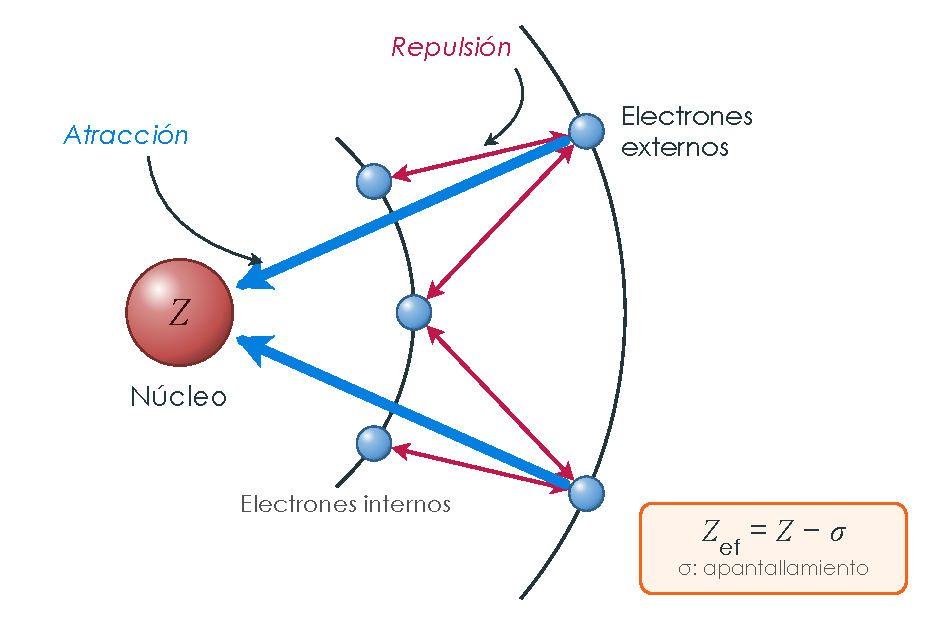
\includegraphics[width=0.65\linewidth]{FigurasSVG/UD2_Tabla_Periodica/pdf/UD2_01_apantallamiento.pdf}
            \caption{Apantallamiento de electrones}
            \label{fig:apantallamiento}
        \end{figure}
        El efecto pantalla no tiene sentido estimarlo entre los elementos de un mismo período porque todos los elementos tienen ocupado el mismo nivel energético.
        El efecto pantalla sí tiene sentido estudiarlo entre los elementos de un mismo grupo, ya que al ir bajando en el grupo, aumentarán los niveles energéticos llenados y, por tanto, el apantallamiento es mayor.
        \item \negrita{Capa de valencia}: capa en la que se encuentran los electrones más externos de un átomo.
        \item \negrita{Carga nuclear efectiva (\(\bm{Z_{eff}}\))}: es la carga nuclear teniendo en cuenta el apantallamiento y hace referencia a cómo los electrones están atraídos por el núcleo. Al $\uparrow\;Z_{eff}$ los electrones estarán más atraídos, mientras que si $\downarrow\;Z_{eff}$ los electrones estarán menos atraídos por el núcleo.
        La carga nuclear efectiva puede calcularse según la ecuación:
        \begin{centeredequation}
            Z_{eff} = Z - \sigma
        \end{centeredequation}

\end{enumerate}

\subsection{Radio atómico}\label{subsec:radio-atomico}

\begin{center}
    \begin{definition}[Radio atómico]
        Se puede definir como la distancia que separa el núcleo del átomo de su electrón más periférico.
        También lo podemos definir como la mitad de la distancia entre dos núcleos de átomos idénticos.
    \end{definition}
\end{center}

La variación del radio atómico está justificada por los siguientes factores:

\begin{enumerate}[label=\numberballmDarkTeal]
        \item Al aumentar la \textbf{carga nuclear}, el radio atómico tiende a ser menor, ya que aumenta la atracción electrostática del núcleo sobre la nube electrónica y hace que esta se aproxime más.
        Es el efecto más notorio en un período.
        \item Al descender en un grupo, aumenta el \textbf{efecto pantalla} y el radio atómico también aumenta.
        Al incrementarse el número de capas, aumenta la repulsión entre los electrones (aumenta el apantallamiento), por lo que su carga nuclear efectiva es menor y la nube electrónica se expande.
        Esto quiere decir que al bajar en un grupo hay más niveles energéticos con electrones, estos se repelen entre sí y, por tanto, se atraen menos por el núcleo, aumentando así el radio atómico.
        \item Al aumentar la \textbf{capa de valencia}, el radio atómico es \textbf{mayor}.
        La capa de valencia aumenta al descender en un grupo y no varía dentro de un período.
\end{enumerate}
% \begin{enumerate}[label=\numberballmDarkTeal]
%     \item \negrita{Grupo}: los radios atómicos crecen al aumentar el número atómico (al bajar en el grupo) y se debe a:
%     \begin{enumerate}
%         \item Al aumentar $Z$ tendremos un mayor número de electrones y por tanto el apantallamiento será mayor por lo que su $Z_{eff}$ será menor (los electrones menos atraídos por el núcleo).
%         \item Al bajar en el grupo aumentamos también el número de niveles y por lo tanto los electrones se encontrarán más alejados del número.
%     \end{enumerate}
%     \item \negrita{Periodo}: al ir de izquierda a derecha la carga nuclear irá aumentando y por lo tanto habrá más electrones que estarán mas atraídos por el núcleo disminuyendo así su radio. Aquí no tenemos en cuenta el apantallamiento porque al tener todos los mismos números de niveles energéticos el apantallamiento es similar.
% \end{enumerate}
Podemos decir que el radio atómico aumenta al descender en un grupo y al desplazarnos a la izquierda en un período, a excepción de los gases nobles.
Es decir, un átomo será tanto mayor cuanto más bajo y a la izquierda en la tabla periódica se encuentre el elemento correspondiente.
\begin{figure}[H]
    \centering
    % [FIGURA ORIGINAL] \includegraphics[scale=0.2]{images/imagesUD2TablaPeriodica/UD2_Teoria/variacionradio4}
    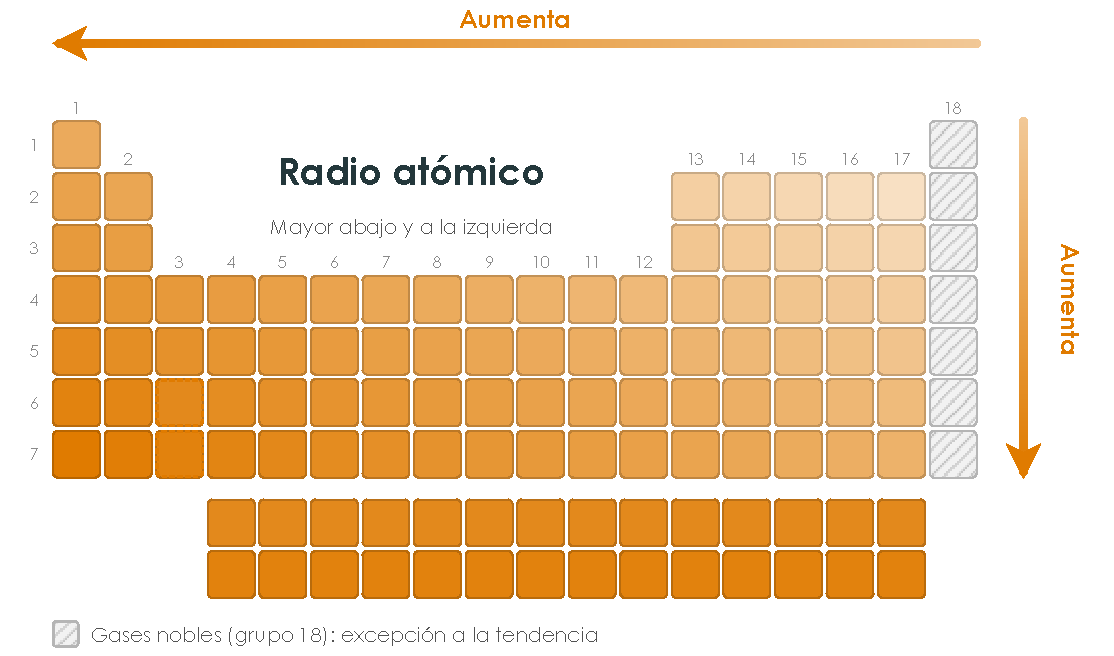
\includegraphics[width=0.85\linewidth]{FigurasSVG/UD2_Tabla_Periodica/pdf/UD2_02_variacion_radio_atomico.pdf}
    \caption{Variación del radio}
    \label{fig:variacionradio3}
\end{figure}

\subsubsection{Radio atómico en iones}

\begin{enumerate}[label=\numberballmDarkTeal]
        \item \negrita{Cationes}: tendrán siempre un radio \textbf{menor} que los elementos neutros, debido a que al perder un electrón, la atracción por el núcleo será mayor y, por tanto, disminuirá el radio.
        \item \negrita{Aniones}: tienen un radio \textbf{mayor} que los elementos neutros, ya que al aumentar el número de electrones, aumentará la repulsión disminuyendo así la atracción de los electrones por el núcleo.
\end{enumerate}
\begin{figure}[H]
    \centering
    % [FIGURA ORIGINAL] \includegraphics[scale=0.75]{images/imagesUD2TablaPeriodica/UD2_Teoria/variacioncationesaniones}
    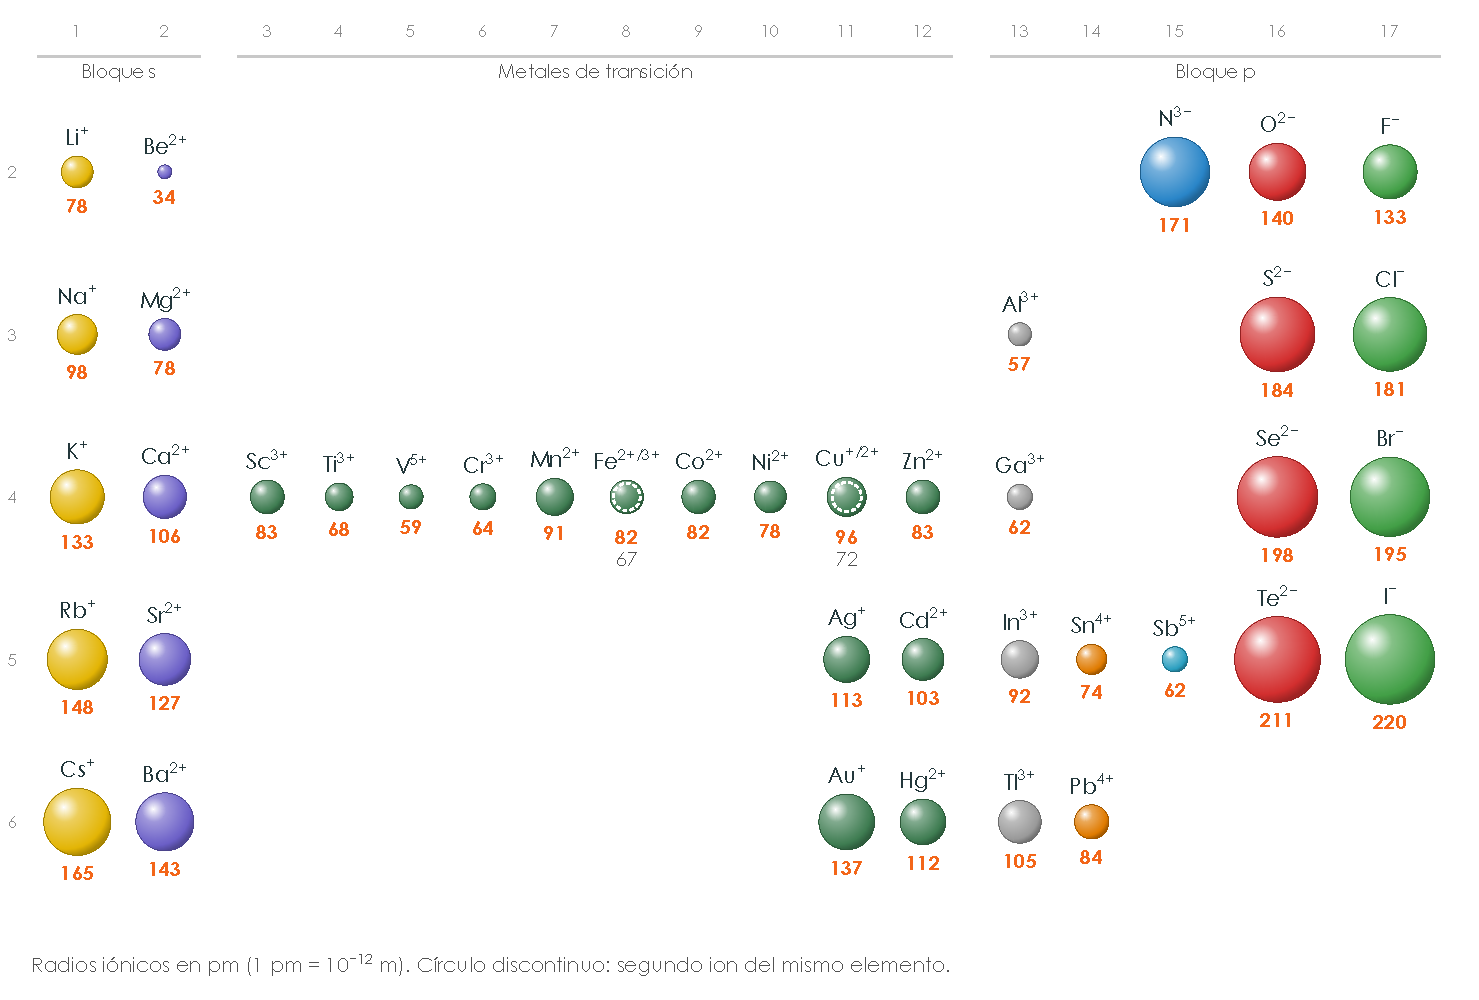
\includegraphics[width=1.0\linewidth]{FigurasSVG/UD2_Tabla_Periodica/pdf/UD2_03_radios_ionicos.pdf}
    \caption{Variación de cationes y aniones}
    \label{fig:variacioncationes}
\end{figure}

\subsection{Energía de ionización o potencial de ionización}\label{subsec:energia-de-ionizacion-o-potencial-de-ionizacion}


\begin{definition}[Energía de ionización (EI) o potencial de ionización (PI)]
        Es la energía necesaria para arrancar un electrón a un átomo en estado gaseoso.
        \begin{centeredequation}
             X(g)\longrightarrow X^+ (g) + e^-
        \end{centeredequation}
        Se mide en unidades de energía: \unit{\kilo\joule\per\mole}, \unit{\joule\per \text{átomo}}, \unit{\electronvolt\per \text{átomo}}.
\end{definition}

Los valores de las energías de ionización tienen signos positivos debido a que hay que administrar energía para provocar la eliminación de un electrón.

El primer electrón que se arranca es más fácil de extraer que el segundo y así sucesivamente, por lo que sus potenciales o energías de ionización van aumentando porque los electrones están cada vez más atraídos por el núcleo (1º PI \(<\) 2º PI \(<\) 3º PI ...).

La variación de la EI se justifica según los siguientes factores:

\begin{enumerate}[label=\numberballmDarkTeal]
        \item El potencial de ionización será mayor al aumentar la carga nuclear efectiva, puesto que los electrones están más atraídos por el núcleo.
        \item Al descender en un grupo, se intensifica el \textbf{efecto pantalla}, lo que provoca que disminuya la carga nuclear efectiva, disminuyendo así el potencial de ionización.
        \item Al avanzar en un período, aumenta la \textbf{carga nuclear}, aumentando así la atracción de los electrones por el núcleo, siendo más difícil extraer un electrón, lo que implica un mayor potencial de ionización.
        \item Al aumentar la capa de valencia (bajamos en un grupo), los electrones están más alejados del núcleo y, por ello, se necesita menos energía para arrancarlos.
\end{enumerate}
% \begin{enumerate}[label=\numberballmDarkTeal]
%     \item \negrita{Grupo}: al bajar en un grupo disminuye su EI ya que la carga nuclear efectiva será menor al ser el apantallamiento mayor y por tanto los electrones están menos atraídos por el núcleo.
%     \item \negrita{Periodo}: al ir de izquierda a derecha, la carga nuclear aumenta por lo que los electrones están más atraídos por el núcleo y por tanto su EI de ionización será mayor.
% \end{enumerate}

Podemos decir que el potencial de ionización aumenta al subir en un grupo y al desplazarse a la derecha del período, es decir, cuanto más arriba y a la derecha de la tabla periódica.

\begin{figure}[H]
    \centering
    % [FIGURA ORIGINAL] \includegraphics[scale=0.2]{images/imagesUD2TablaPeriodica/UD2_Teoria/variacionei2}
    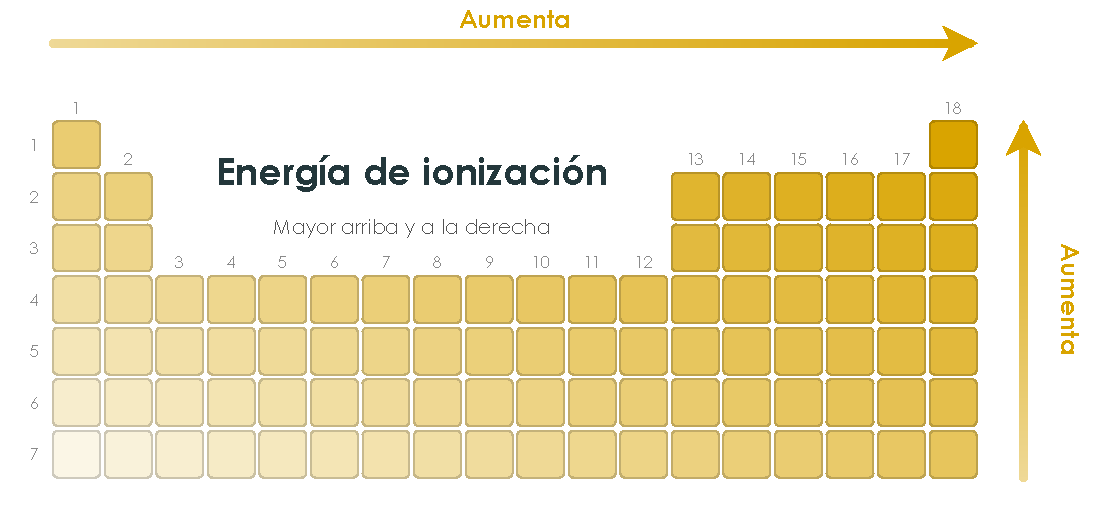
\includegraphics[width=0.85\linewidth]{FigurasSVG/UD2_Tabla_Periodica/pdf/UD2_04_variacion_energia_ionizacion.pdf}
    \caption{Variación de la EI}
    \label{fig:variacionei}
\end{figure}

A continuación, tenemos una tabla con los valores de EI. Como podemos apreciar, existe una anomalía entre la EI del \ch{Be} y el \ch{B}, que se debe a que el \ch{Be} tiene su capa de valencia llena y, por tanto, su tendencia a perder electrones es menor que en el caso del boro, que tiene un electrón en el orbital \( p \).
Algo similar ocurre entre el nitrógeno y el oxígeno.

\begin{table}[H]
    \centering
    \caption{Variación de la energía de ionización}
    \vspace*{-8pt}
    % --- tabla antigua ---
    % \begin{tblr}{|c|c|c|c|c|c|c|c|c|}
        % \hline
        % \SetColumn{mybluecolour} \textbf{\textcolor{white}{Elemento}} & \textbf{\ch{Li}} & \textbf{\ch{Be}} & \textbf{\ch{B}} & \textbf{\ch{C}} & \textbf{\ch{N}} & \textbf{\ch{O}} & \textbf{\ch{F}} & \textbf{\ch{Ne}}   \\
        % \hline
        % \textbf{\textcolor{white}{Valor (eV)}}:                       & 5.38             & 9.25             & 8.26            & 11.22           & 14.48           & 13.65           & 17.34           & 21.45            \\
        % \hline
    % \end{tblr}
    % --- tabla nueva ---
    \begin{tabular}{@{}ccccccccc@{}}
        \toprule
        \SetColumn{mybluecolour} \textbf{\textcolor{white}{Elemento}} & \textbf{\ch{Li}} & \textbf{\ch{Be}} & \textbf{\ch{B}} & \textbf{\ch{C}} & \textbf{\ch{N}} & \textbf{\ch{O}} & \textbf{\ch{F}} & \textbf{\ch{Ne}} \\[3pt]
        \textbf{\textcolor{white}{Valor (eV)}}: & 5.38 & 9.25 & 8.26 & 11.22 & 14.48 & 13.65 & 17.34 & 21.45 \\
        \bottomrule
    \end{tabular}
\end{table}
% \begin{figure}[H]
%     \centering
%     \includegraphics[scale=1]{images/UD2/ei1.png}
%     \caption{Variación EI}
%     \label{fig:variacionei2}
% \end{figure}
\begin{table}[H]
    \centering
    \caption{Configuración electrónica del Be, N, B y O}
    \vspace*{-8pt}
    % --- tabla antigua ---
    % \begin{tblr}[caption = {Configuración electrónica},]{|c|c|}
        % \hline
        % \textbf{\ch{Be}}: \elconf{Be} & \textbf{\ch{N}}: \elconf{N} \\
        % \hline
        % \textbf{\ch{B}}: \elconf{B}   & \textbf{\ch{O}}: \elconf{O} \\
        % \hline
    % \end{tblr}
    % --- tabla nueva ---
    \begin{tabular}{@{}cc@{}}
        \toprule
        \textbf{\ch{Be}}: \elconf{Be} & \textbf{\ch{N}}: \elconf{N} \\[3pt]
        \textbf{\ch{B}}: \elconf{B} & \textbf{\ch{O}}: \elconf{O} \\
        \bottomrule
    \end{tabular}
\end{table}
% \begin{figure}[H]
%     \centering
%     \includegraphics[scale=1]{images/UD2/ei2.png}
%     \caption{Configuración electrónica}
%     \label{fig:configuracionele}
% \end{figure}
\begin{consejo}[Analizar la tendencia del Radio y PI/EI]
    \begin{enumerate}
        \item Estas dos propiedades siempre se analizan teniendo en cuenta la carga nuclear y/o la carga nuclear efectiva.
        \item Cuando analicemos los elementos que están en un mismo período, se utilizará la \textbf{carga nuclear} como referencia, puesto que todos esos elementos tienen el mismo nivel energético con electrones y, por tanto, no tiene sentido hablar de apantallamiento (\(\sigma\)). En este caso debemos decir que, al aumentar el número atómico, aumentará la carga nuclear, quedando, en consecuencia, los electrones más atraídos por el núcleo.
        \item En el caso de que estemos analizando elementos del mismo grupo, hay que justificar su tendencia utilizando la carga nuclear efectiva, \(Z_{eff}\), ya que en este caso, al bajar en el grupo vamos aumentando los niveles energéticos, lo que aumenta el número de electrones y, por tanto, el apantallamiento será mayor (repulsión entre electrones).
        Cuando bajamos en un grupo, aumenta el apantallamiento, disminuyendo así la carga nuclear efectiva (recordamos que \(Z_{eff} = Z - \sigma\)).
    \end{enumerate}
\end{consejo}


\begin{example}
    Dados los elementos K (Z=19), Ca (Z=20), Zn (Z=30), F (Z=9) y Ne (Z=10), ordénalos razonadamente, de menor a mayor, de acuerdo con sus valores de: a) radio atómico; b) energía de ionización.

        {\negsubro{Solución:}}

    Lo primero que debemos hacer es situar el grupo y el período de cada elemento. Ayuda mucho poner la configuración de su capa de valencia, es decir, la configuración electrónica del último nivel ocupado.
    \begin{itemize}
        \item \ch{K}: \elconf{K}
        \item \ch{Ca}: \elconf{Ca}
        \item \ch{Zn}: \elconf{Zn}
        \item \ch{F}: \elconf{F}
        \item \ch{Ne}: \elconf{Ne}
    \end{itemize}

    \begin{enumerate}[label=\letraminuscula]
            \item Ordenación según el radio atómico.

            Aquí tenemos uno de los casos más complejos en los que nos podemos encontrar. Tenemos tres elementos que están en el período 4 (K, Ca y Zn) y otros elementos que están en el período 2 (F y Ne).
            Sabemos que al bajar en la tabla periódica, aumenta la carga nuclear, pero también aumenta el apantallamiento (más electrones que provocan repulsiones), provocando que la carga nuclear efectiva sea menor \( Z_{eff} = Z - \sigma \).
            Si disminuye la carga nuclear efectiva, los electrones estarán menos atraídos por el núcleo y, por tanto, su radio atómico aumentará.
            Llegados a este punto, podemos decir que los elementos K, Ca y Zn tendrán un radio atómico mayor que los elementos F y Ne.
            Los que tendrán menor radio serán el \ch{F} y el \ch{Ne}.
            Ambos están en el mismo período y, por tanto, no tiene sentido hablar de apantallamiento.
            Al tener el \ch{Ne} mayor número atómico, tendrá una mayor carga nuclear y, por tanto, los electrones estarán más atraídos por el núcleo, lo que hará que tenga un radio atómico menor que el del \ch{F}.
            Por lo tanto, \( \ch{Ne} < \ch{F} \).

            Ahora ordenemos los elementos \ch{K}, \ch{Ca} y \ch{Zn}.
            Estos también están todos en el mismo período. El de menor radio será el \ch{Zn}, ya que tiene una mayor carga nuclear, seguido del \ch{Ca} y finalmente el \ch{K}.

            Finalmente, la ordenación por radio atómico quedará de la siguiente manera:
            \[
                \ch{Ne} < \ch{F} < \ch{Zn} < \ch{Ca} < \ch{K}
            \]
            \item Ordenación de la energía de ionización.

            El grupo de los elementos \ch{K}, \ch{Ca} y \ch{Zn} tendrá una energía de ionización menor que los del grupo \ch{F} y \ch{Ne}, ya que los primeros tienen una carga nuclear efectiva menor que los otros y, por tanto, los electrones están menos atraídos por el núcleo, lo que facilita la extracción de un electrón, necesitándose así menor energía (menor energía de ionización).

            Vamos a ordenar primero este grupo.
            Al estar los tres en el mismo período, \ch{K} será el que tenga menor energía de ionización, ya que su carga nuclear es menor y, por tanto, los electrones estarán menos atraídos por el núcleo, luego le sigue el \ch{Ca} y luego el \ch{Zn}.
            Quedando este grupo como \( \ch{K} < \ch{Ca} < \ch{Zn} \).

            Ahora pasamos al grupo del \ch{F} y el \ch{Ne}.
            El \ch{Ne} tiene mayor carga nuclear, lo que incrementa la atracción de los electrones y, por tanto, una mayor energía de ionización (\( \ch{F} < \ch{Ne} \)).

            El resultado final quedará, por tanto, como:
            \begin{equation*}
                \ch{K} < \ch{Ca} < \ch{Zn} < \ch{F} < \ch{Ne}
            \end{equation*}
    \end{enumerate}
\end{example}

\subsection{Afinidad electrónica (AE)}

\begin{definition}[Afinidad electrónica (AE)]
        Es la energía involucrada cuando un átomo en estado gaseoso capta un electrón, formándose un ion negativo.
        \begin{centeredequation}
           X(g) + e^- \longrightarrow X^- (g)
        \end{centeredequation}
        Se mide en unidades de energía: \unit{\kilo\joule\per\mole}, \unit{\joule\per \text{átomo}}, \unit{\electronvolt\per \text{átomo}}.
\end{definition}

El signo negativo de estas AE indica que se trata de una energía desprendida cuando el átomo capta un electrón.
Los elementos con AE positivas no muestran tendencia a captar electrones.

También se puede dar el caso de una segunda o tercera AE, estos casos son difíciles de calcular y no tienen una variación regular.

\begin{enumerate}[label=\numberballmDarkTeal]
        \item En un grupo como en un período, al aumentar la carga nuclear se eleva la atracción electrostática del núcleo sobre el electrón y se libera más energía, es decir, la AE es mayor.
        \item Al descender en un grupo, se intensifica el \textbf{efecto pantalla}, provocando así una disminución de la carga nuclear efectiva, liberándose menor energía al capturar el electrón, lo que provoca una disminución de la AE.
        \item Al aumentar la capa de valencia, el electrón que se capta estará más alejado del núcleo, experimentando una menor atracción y, por tanto, una menor AE.
\end{enumerate}
% \begin{enumerate}[label=\numberballmDarkTeal]
%     \item \negrita{Grupo}: En un grupo, el valor de la AE disminuye al bajar en el grupo. En la siguiente table se muestra un valor anómalo para el \ch{F} debido a que este es más pequeño y la adición de un electrón provoca un aumento en la repulsión. Los valores están dados en valores absolutos.
%     \begin{figure}[H]
%         \centering
%         \includegraphics[scale=1]{aetabla.png}
%         \caption{Valores de AE}
%         \label{fig:valoresddeae}
%     \end{figure}
%     \item \negrita{Periodo}: aumenta de izquierda a derecha
% \end{enumerate}
Podemos decir que la AE aumenta al subir en un grupo y al desplazarse a la derecha en un período, a excepción de los gases nobles, es decir, es mayor cuanto más arriba y más a la derecha de la tabla periódica.
\begin{figure}[H]
    \centering
    % [FIGURA ORIGINAL] \includegraphics[scale=0.2]{images/imagesUD2TablaPeriodica/UD2_Teoria/variacionae2.png}
    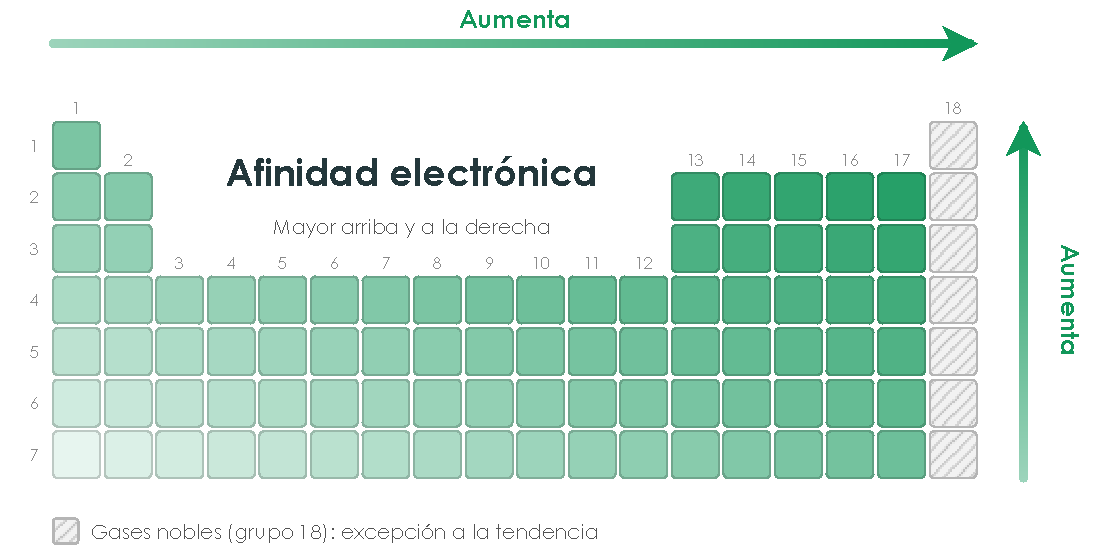
\includegraphics[width=0.85\linewidth]{FigurasSVG/UD2_Tabla_Periodica/pdf/UD2_05_variacion_afinidad_electronica.pdf}
    \caption{Variación de la AE}
    \label{fig:variacionae}
\end{figure}

\subsection{Electronegatividad}

    \begin{definition}[Electronegatividad (EN)]
        Es la tendencia que tiene un átomo a atraer hacia sí los electrones de un enlace químico.
        Se puede expresar en unidades de energía como \unit{\kilo\joule\per\mole}, pero es habitual expresarlo en una escala arbitraria que da una idea cualitativa de esa tendencia.
    \end{definition}

Es muy importante no confundir la electronegatividad con la afinidad electrónica.
Debemos tener en cuenta que la electronegatividad se debe a la tendencia de un átomo a llevarse los electrones cuando están formando un enlace mientras que la afinidad electrónica es la tendencia que tiene un átomo a ganar un electrón.

\begin{enumerate}[label=\numberballmDarkTeal]
        \item \negrita{Grupo}: disminuye a medida que aumenta el número atómico.
        \item \negrita{Periodo}: aumenta de izquierda a derecha.
\end{enumerate}

La \textbf{electronegatividad} aumenta al subir en un grupo y al desplazarse a la derecha en un período, a excepción de los gases nobles, es decir, es mayor cuanto más arriba y a la derecha de la tabla periódica se encuentre el elemento químico.
\begin{figure}[H]
    \centering
    % [FIGURA ORIGINAL] \includegraphics[scale=0.2]{images/imagesUD2TablaPeriodica/UD2_Teoria/variacionelectronegatividad2.png}
    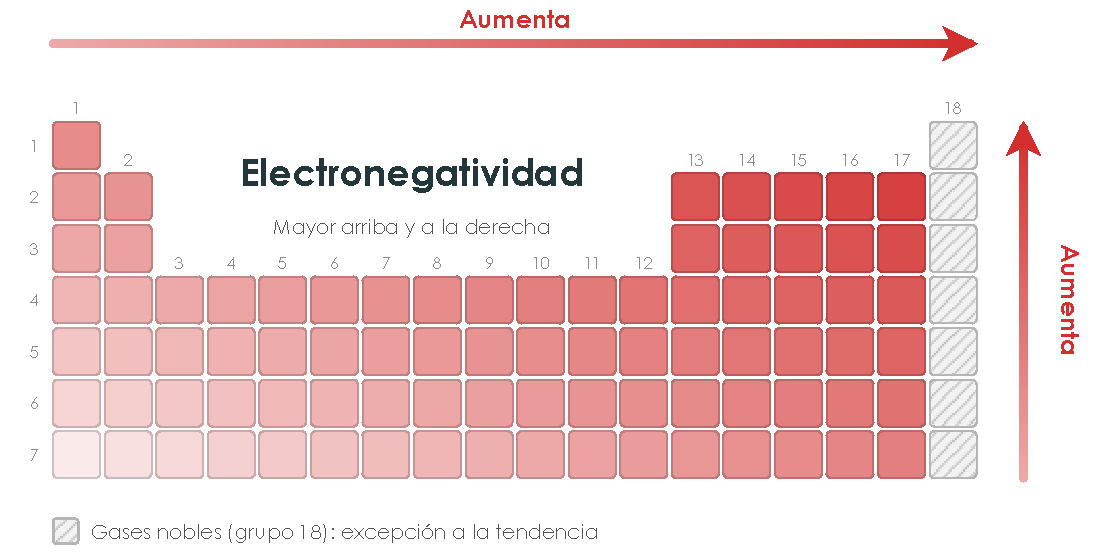
\includegraphics[width=0.85\linewidth]{FigurasSVG/UD2_Tabla_Periodica/pdf/UD2_06_variacion_electronegatividad.pdf}
    \caption{Variación de la electronegatividad}
    \label{fig:variacionelectronegatividad}
\end{figure}

Los valores de la electronegatividad se pueden obtener según la expresión:
\begin{centeredequation}
     \text{Electronegatividad} = \dfrac{EI + AE}{2}
\end{centeredequation}
A modo informativo, en la figura \ref{fig:tabla de electronegatividades de Pauling} tenemos una tabla con el valor de las electronegatividades de los elementos.

\begin{figure}[H]
    \centering
    % [FIGURA ORIGINAL] \includegraphics[scale=.3]{images/imagesUD2TablaPeriodica/UD2_Teoria/pauling electronegativity table_b.png}
    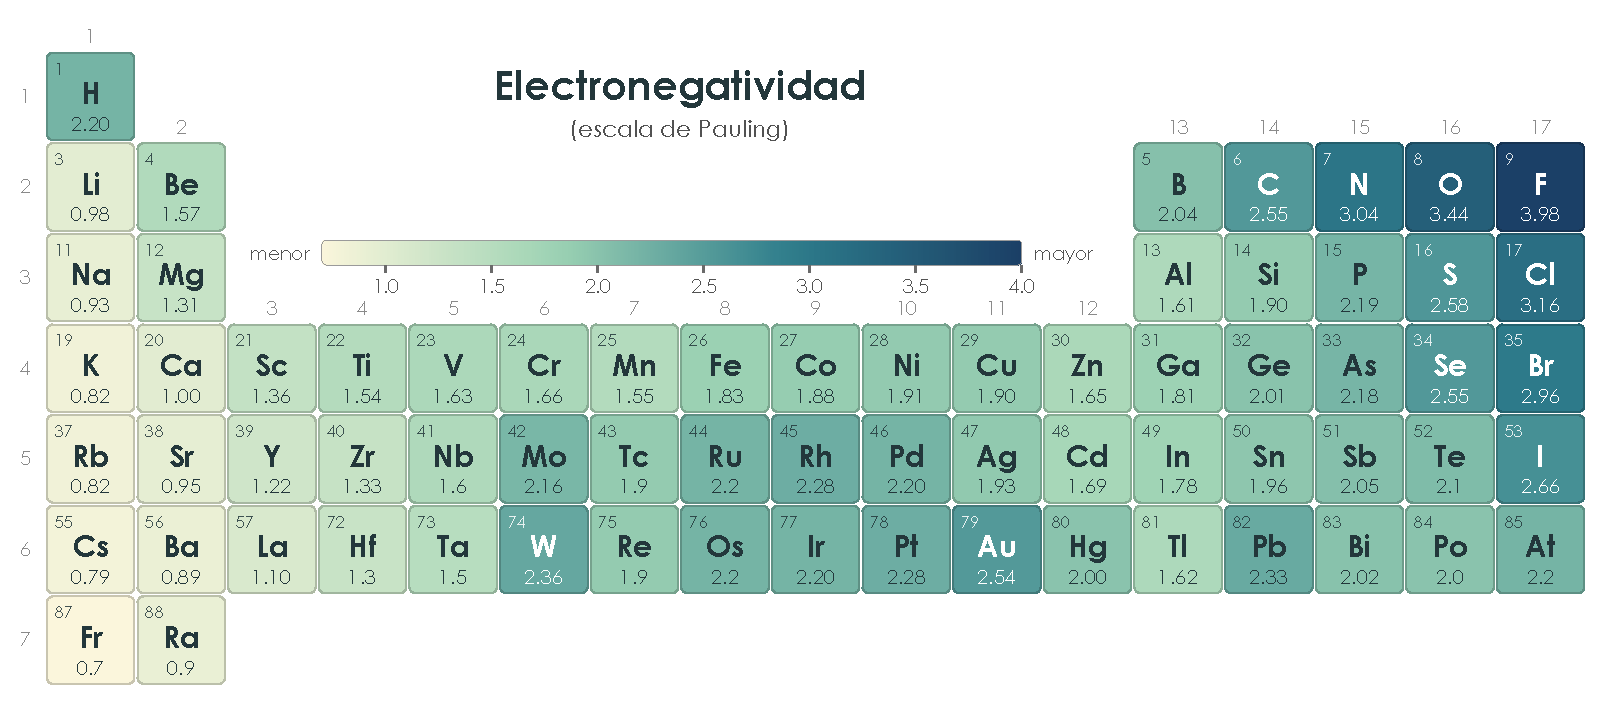
\includegraphics[width=1.0\linewidth]{FigurasSVG/UD2_Tabla_Periodica/pdf/UD2_07_tabla_electronegatividades_pauling.pdf}
    \caption{Tabla de electronegatividades de Pauling}
    \label{fig:tabla de electronegatividades de Pauling}
\end{figure}

\subsection{Otras propiedades químicas y físicas}

\begin{enumerate}[label=\numberballmDarkTeal]
        \item \negsubro{Número de oxidación}. Es una consecuencia directa de la configuración electrónica y, por lo tanto, de la situación de un elemento en la TP.
        \item \negsubro{Carácter metálico}. El carácter metálico lo podemos definir a partir de la electronegatividad.
        Los elementos metálicos tienen tendencia a ceder electrones.
        Los elementos con bajos potenciales de ionización y bajas afinidades electrónicas tendrán más carácter metálico.
\end{enumerate}




    \newpage

    \setcounter{cuestion}{0}
\setcounter{ejerciciogeneral}{0}
\setcounter{ejercicionumero}{0}

%\booltrue{soluciones}


\section{Ejercicios}

\subsection{Cuestiones}

\begin{question}
    Ordena los siguientes elementos según el tamaño creciente
    de sus átomos y justifica la respuesta: Si, Ne, F, Mg, S, K.

    \begin{solu}
        Debemos tener en cuenta la carga nuclear y la configuración
        de valencia de cada átomo:

%        \begin{figure}[H]
%            \centering
%            \includegraphics[scale=1]{images/imagesUD2TablaPeriodica/UD2_Problemas/cuestion1}
%            %\caption{}
%            %\label{fig:}
%        \end{figure}

        \begin{center}
            % --- tabla antigua ---
            % \begin{tblr}{hlines, vlines, colspec={Q[l,m,wd=2.9cm] c c c c c c}, row{1}={bg=mybluecolour!15, font=\bfseries}, column{1}={font=\bfseries}}
                                          % & \ch{Si}               & \ch{Ne}               & \ch{F}                & \ch{Mg}          & \ch{S}                & \ch{K}           \\
                % \(Z\)                     & 14                    & 10                    & 9                     & 12               & 16                    & 19               \\
                % Configuración de valencia & \(\mathrm{3s^2\,3p^2}\) & \(\mathrm{2s^2\,2p^6}\) & \(\mathrm{2s^2\,2p^5}\) & \(\mathrm{3s^2}\) & \(\mathrm{3s^2\,3p^4}\) & \(\mathrm{4s^1}\) \\
            % \end{tblr}
            % --- tabla nueva ---
            \begin{tabular}{@{}L{2.9cm} c c c c c c@{}}
                \toprule
                 & \textbf{\ch{Si}} & \textbf{\ch{Ne}} & \textbf{\ch{F}} & \textbf{\ch{Mg}} & \textbf{\ch{S}} & \textbf{\ch{K}} \\
                \midrule
                \textbf{\(Z\)} & 14 & 10 & 9 & 12 & 16 & 19 \\[3pt]
                \textbf{Configuración de valencia} & \(\mathrm{3s^2\,3p^2}\) & \(\mathrm{2s^2\,2p^6}\) & \(\mathrm{2s^2\,2p^5}\) & \(\mathrm{3s^2}\) & \(\mathrm{3s^2\,3p^4}\) & \(\mathrm{4s^1}\) \\
                \bottomrule
            \end{tabular}
        \end{center}

        El mayor tamaño lo tiene el K, pues sus electrones de valencia
        están en la capa más alejada del núcleo (mayor número cuántico
        principal), lo que pesa más que el aumento de la carga nuclear.

        Para los elementos que están en un mismo período (Mg, Si, S), la
        capa de valencia es la misma, por lo que la comparación depende
        de la carga nuclear efectiva, \(Z_{ef} = Z - \sigma\), siendo
        \(\sigma\) el apantallamiento que ejercen los electrones internos.
        Al recorrer el período de izquierda a derecha, la carga nuclear
        \(Z\) aumenta en una unidad por cada elemento, mientras que el
        apantallamiento de los electrones internos apenas varía; por
        ello, \(Z_{ef}\) crece a lo largo del período. Cuanto mayor es
        \(Z_{ef}\), mayor es la atracción del núcleo sobre los electrones
        de valencia y menor el tamaño de la corteza electrónica. El
        mismo razonamiento se aplica a F y Ne, que pertenecen al
        período 2.
        En consecuencia, el orden creciente es el siguiente:

        \[K > Mg > Si > S > F > Ne\]
    \end{solu}
\end{question}

\begin{question}
    Razona si es cierto que un ion siempre tiene un tamaño
    menor que el del átomo correspondiente.

    \begin{solu}
        El catión tiene menor tamaño que el átomo correspondiente,
        pero el anión es más grande que su átomo.
    \end{solu}
\end{question}

\begin{question}
    Ordena los siguientes elementos químicos por su radio
    atómico: Se, Br, Kr, Rb y Sr. Determina la configuración
    electrónica del ion más estable que se puede formar
    con cada uno de estos átomos y ordena dichos iones
    según su radio.


    \begin{solu}

%        \begin{figure}[H]
%            \centering
%            \includegraphics[scale=1]{ images/imagesUD2TablaPeriodica/UD2_Problemas/cuestion3.png}
%            %\caption{}
%            %\label{fig:}
%        \end{figure}

        Tienen mayor tamaño los elementos del período 5 (Rb, Sr) que los
        del 4 (Se, Br, Kr), porque sus electrones de valencia están más
        alejados del núcleo, lo que prevalece sobre el efecto de la
        carga nuclear. Dentro de cada período, el apantallamiento
        \(\sigma\) que ejercen los electrones internos es prácticamente
        el mismo para todos los elementos, mientras que la carga
        nuclear \(Z\) aumenta con el número atómico; por ello, la carga
        nuclear efectiva \(Z_{ef} = Z - \sigma\) crece a lo largo del
        período. Cuanto mayor es \(Z_{ef}\), mayor es la atracción que
        el núcleo ejerce sobre los electrones más periféricos y menor
        el radio atómico:
        \[Rb > Sr > Se > Br > Kr\]

        Los iones más estables de estos elementos son \(\ch{Se^2-}\),
        \(\ch{Br-}\), \(\ch{Kr}\) (no forma iones estables), \(\ch{Rb+}\)
        y \(\ch{Sr^2+}\), todos con la configuración electrónica de gas
        noble del \ch{Kr}. Al tener todos ellos el mismo número de
        electrones (36) e idéntico apantallamiento, el radio del ion
        depende únicamente de la carga nuclear: cuanto mayor es \(Z\),
        mayor es \(Z_{ef}\) sobre esos 36 electrones y menor el radio
        iónico. Como \(\ch{Se^2-}\) tiene la menor carga nuclear
        (\(Z=34\)) y \(\ch{Sr^2+}\) la mayor (\(Z=38\)), el orden
        creciente de radio iónico es:
        \[\ch{Sr^2+} < \ch{Rb+} < \ch{Br-} < \ch{Se^2-}\]
    \end{solu}
\end{question}

\begin{question}
    Justifica por qué los elementos de transición de un mismo
    período tienen tamaños tan parecidos.


    \begin{solu}
        Tienen tamaños tan parecidos porque todos poseen la misma
        configuración electrónica en su capa más exterior; el electrón
        diferenciador se sitúa en una capa más interior. Por otra
        parte, su número atómico es lo suficientemente alto como
        para que no sea muy significativa la presencia de un protón
        más en el núcleo del átomo de cada elemento.
    \end{solu}

\end{question}

\begin{question}
    Indica por qué no es correcta la siguiente definición:
    «El potencial de ionización es la energía que hay que
    comunicar a un átomo para arrancarle un electrón».


    \begin{solu}
        No es correcta la afirmación porque hay que precisar que el
        átomo debe estar aislado y que el electrón ha de hallarse en
        la capa de valencia del átomo
    \end{solu}

\end{question}

\begin{question}
    ¿Cuántas energías de ionización se pueden establecer
    en el caso del aluminio?

    \begin{solu}
        Para el aluminio se pueden establecer 13 energías de ionización,
        ya que tiene 13 electrones.
    \end{solu}

\end{question}

\begin{question}
    Explica por qué el segundo potencial de ionización de
    un elemento químico tiene el mismo signo que el primero,
    y la segunda afinidad electrónica, signo contrario
    a la primera.


    \begin{solu}
        El potencial de ionización es la energía que hay que comunicar
        a un átomo en estado gaseoso para arrancarle un electrón.
        Si se trata del segundo electrón, será el segundo potencial
        de ionización y habrá que comunicarle aún más energía
        para arrancárselo.

        La afinidad electrónica, por su parte, es la energía que desprende
        el átomo en estado gaseoso cuando capta un electrón. Si se trata del segundo electrón, será la segunda afinidad electrónica, pero un átomo nunca cederá energía al captar un
        segundo electrón; por el contrario, si se quiere que suceda
        esto habrá que comunicársela. Por eso, la segunda afinidad
        electrónica siempre tiene signo contrario a la primera.

    \end{solu}

\end{question}

\begin{question}
    El litio, el sodio y el potasio son tres metales alcalinos de
    número atómico 3, 11 y 19, respectivamente. Asigna de
    manera razonada a cada uno de estos metales uno de
    los siguientes valores posibles para la energía de ionización:
    100 kcal/mol, 119 kcal/mol y 124 kcal/mol.


    \begin{solu}
        Debemos tener en cuenta la carga nuclear y la configuración
        de valencia de cada átomo:

%        \begin{figure}[H]
%            \centering
%            \includegraphics[scale=1]{ images/imagesUD2TablaPeriodica/UD2_Problemas/cuestion8.png}
%            %\caption{}
%            %\label{fig:}
%        \end{figure}

        \begin{center}
            % --- tabla antigua ---
            % \begin{tblr}{hlines, vlines, colspec={l c c c}, row{1}={bg=mybluecolour!15, font=\bfseries}, column{1}={font=\bfseries}}
                                                                   % & \ch{Li}           & \ch{Na}           & \ch{K}            \\
                % \(Z\)                                              & 3                 & 11                & 19                \\
                % Configuración de valencia                          & \(\mathrm{2s^1}\) & \(\mathrm{3s^1}\) & \(\mathrm{4s^1}\) \\
                % Energía de ionización (\unit{\kilo\calorie\per\mole}) & 124               & 119               & 100               \\
            % \end{tblr}
            % --- tabla nueva ---
            \begin{tabular}{@{}lccc@{}}
                \toprule
                 & \textbf{\ch{Li}} & \textbf{\ch{Na}} & \textbf{\ch{K}} \\
                \midrule
                \textbf{\(Z\)} & 3 & 11 & 19 \\[3pt]
                \textbf{Configuración de valencia} & \(\mathrm{2s^1}\) & \(\mathrm{3s^1}\) & \(\mathrm{4s^1}\) \\[3pt]
                \textbf{Energía de ionización (\unit{\kilo\calorie\per\mole})} & 124 & 119 & 100 \\
                \bottomrule
            \end{tabular}
        \end{center}

        La energía de ionización es la que se requiere para arrancar
        el electrón de valencia a un mol de átomos del elemento en
        estado gaseoso. Todos estos elementos tienen un único electrón
        de valencia, pero situado en capas distintas (2, 3 y 4,
        respectivamente); al ser todos alcalinos, la carga nuclear
        efectiva sobre ese electrón de valencia es similar en los tres
        (\(Z_{ef} \approx +1\), ya que el resto de electrones internos
        apantalla casi por completo el aumento de \(Z\)), por lo que el
        factor decisivo es la distancia al núcleo. Resultará más fácil
        arrancárselo al potasio, pues en su caso ese electrón se
        encuentra en una capa más alejada del núcleo que en cualquiera
        de los otros dos. En consecuencia, el potasio tiene la menor
        energía de ionización (100 kcal/mol), seguido del sodio
        (119 kcal/mol) y del litio (124 kcal/mol).


    \end{solu}

\end{question}

\begin{question}
    Ordena según el valor creciente de su primera energía
    de ionización, justificando las posibles anomalías, los
    siguientes elementos: Al, Ne, P, Mg, S y K.


    \begin{solu}
        Debemos tener en cuenta la carga nuclear y la configuración
        de valencia de cada átomo:
%        \begin{figure}[H]
%            \centering
%            \includegraphics[scale=1]{ images/imagesUD2TablaPeriodica/UD2_Problemas/cuestion9}
%            %\caption{}
%            %\label{fig:}
%        \end{figure}

        \begin{center}
            % --- tabla antigua ---
            % \begin{tblr}{hlines, vlines, colspec={Q[l,m,wd=2.9cm] c c c c c c}, row{1}={bg=mybluecolour!15, font=\bfseries}, column{1}={font=\bfseries}}
                                          % & \ch{Al}               & \ch{Ne}               & \ch{P}                & \ch{Mg}          & \ch{S}                & \ch{K}           \\
                % \(Z\)                     & 13                    & 10                    & 15                    & 12               & 16                    & 19               \\
                % Configuración de valencia & \(\mathrm{3s^2\,3p^1}\) & \(\mathrm{2s^2\,2p^6}\) & \(\mathrm{3s^2\,3p^3}\) & \(\mathrm{3s^2}\) & \(\mathrm{3s^2\,3p^4}\) & \(\mathrm{4s^1}\) \\
            % \end{tblr}
            % --- tabla nueva ---
            \begin{tabular}{@{}L{2.9cm} c c c c c c@{}}
                \toprule
                 & \textbf{\ch{Al}} & \textbf{\ch{Ne}} & \textbf{\ch{P}} & \textbf{\ch{Mg}} & \textbf{\ch{S}} & \textbf{\ch{K}} \\
                \midrule
                \textbf{\(Z\)} & 13 & 10 & 15 & 12 & 16 & 19 \\[3pt]
                \textbf{Configuración de valencia} & \(\mathrm{3s^2\,3p^1}\) & \(\mathrm{2s^2\,2p^6}\) & \(\mathrm{3s^2\,3p^3}\) & \(\mathrm{3s^2}\) & \(\mathrm{3s^2\,3p^4}\) & \(\mathrm{4s^1}\) \\
                \bottomrule
            \end{tabular}
        \end{center}
        La energía de ionización es la que se requiere para arrancar
        el electrón de valencia a un mol de átomos del elemento en
        estado gaseoso. Su valor depende de la configuración de la
        capa de valencia y, sobre todo, de la carga nuclear efectiva
        \(Z_{ef} = Z - \sigma\) que percibe el electrón de valencia:
        cuanto mayor es \(Z_{ef}\), con más fuerza lo retiene el átomo y
        mayor es su energía de ionización.
        De todos los presentes, el K es el elemento de menor energía
        de ionización, ya que tiene el electrón de valencia en la capa
        más alejada del núcleo (\(n=4\)) y solo tiene uno, muy apantallado
        por el resto de electrones internos.
        De los elementos que están en el tercer período (Mg, Al, S y P),
        el apantallamiento interno es prácticamente el mismo para todos
        ellos, de modo que \(Z_{ef}\) aumenta con \(Z\) a lo largo del
        período; el Mg es el que tiene menor energía de ionización,
        pues es el que tiene menos protones en su núcleo (menor \(Z\) y,
        por tanto, menor \(Z_{ef}\)). Le sigue el Al. El S tiene
        un protón más en el núcleo que el P; por tanto, se podría
        pensar que su energía de ionización es mayor. No obstante,
        el P tiene estructura de semicapa cerrada (\(3p^13p^13p^1\)), una
        estructura de especial estabilidad que puede alcanzar el S si
        pierde un electrón de valencia; por este motivo, la energía de
        ionización del S es menor que la del P.
        Finalmente, el Ne es el elemento con la energía de ionización
        más alta, ya que tiene estructura de capa cerrada (es un gas
        noble) y es muy difícil que la pierda.
        75
        Sistema periódico de los elementos 2
        Unidades didácticas Química 2.º Bachillerato
        En conclusión, el orden de los elementos según su energía de
        ionización sería, de mayor a menor:
        \[Ne > P > S > Al > Mg > K\]
    \end{solu}

\end{question}

\begin{question}
    Ordena los siguientes elementos según su primer potencial
    de ionización: Br, K, Mg y S. Si atendemos a su segundo potencial de ionización, ¿estarían en el mismo orden?


    \begin{solu}

%        \begin{figure}[H]
%            \centering
%            \includegraphics[scale=1]{ images/imagesUD2TablaPeriodica/UD2_Problemas/cuestion10a.png}
%            %\caption{}
%            %\label{fig:}
%        \end{figure}
%
%        \begin{figure}[H]
%            \centering
%            \includegraphics[scale=1]{ images/imagesUD2TablaPeriodica/UD2_Problemas/cuestion10b.png}
%            %\caption{}
%            %\label{fig:}
%        \end{figure}

        La justificación reside en la configuración electrónica de la
        especie que va a perder el electrón y en la carga nuclear
        efectiva \(Z_{ef} = Z - \sigma\) que actúa sobre ese electrón.

        El Br y el S pertenecen al período 4 y al período 3
        respectivamente, mientras que el K y el Mg se encuentran en el
        mismo período que, en cada caso, el elemento con el que se
        comparan; en todos los casos, cuanto mayor es \(Z_{ef}\) sobre
        el electrón de valencia, mayor es el primer PI.
        El elemento con mayor 1.er PI es el Br, al que solo le falta un
        electrón para alcanzar la configuración de gas noble (elevada
        \(Z_{ef}\) por su posición al final del período) y que,
        por ello, tiene muy poca tendencia a perder electrones; le
        sigue el S, al que le faltan 2 electrones para tener configuración
        de gas noble. Entre estos dos elementos, el S es el que
        tiene mayor segundo PI, ya que posee estructura de semicapa
        cerrada, de especial estabilidad.

        El tercer elemento, en lo que al valor del primer PI se refiere,
        es el Mg, que solo tiene 2 electrones en su capa de valencia,
        poco apantallados frente a la \(Z_{ef}\) que ya ejerce su núcleo.
        Al perder el segundo electrón, adquiere configuración de gas
        noble; por eso, es el elemento que tiene menor segundo PI.

        El 1.er PI más bajo lo tiene el K, ya que su único electrón de
        valencia ocupa la capa \(n=4\), muy alejada del núcleo y muy
        apantallada por el resto de electrones internos (\(Z_{ef}\)
        pequeña); si lo pierde, adquiere configuración de gas noble.
        Por esta razón, es el elemento que
        tiene el segundo PI más alto.
    \end{solu}

\end{question}

\begin{question}
    Las especies H, \ch{He+} y \ch{Li\pch[2]} poseen un solo electrón.
    Razona
    cuál de ellas poseerá: a) la mayor energía de ionización;
    b) el radio más grande.


    \begin{solu}
        Consideramos la carga nuclear de estas especies:
%        \begin{figure}[H]
%            \centering
%            \includegraphics[scale=1]{images/imagesUD2TablaPeriodica/UD2_Problemas/cuestion11.png}
%            %\caption{}
%            %\label{fig:}
%        \end{figure}

        \begin{center}
            % --- tabla antigua ---
            % \begin{tblr}{hlines, vlines, colspec={l c c c}, row{1}={bg=mybluecolour!15, font=\bfseries}, column{1}={font=\bfseries}}
                      % & \ch{H} & \ch{He+} & \ch{Li\pch[2]} \\
                % \(Z\) & 1      & 2        & 3              \\
            % \end{tblr}
            % --- tabla nueva ---
            \begin{tabular}{@{}lccc@{}}
                \toprule
                 & \textbf{\ch{H}} & \textbf{\ch{He+}} & \textbf{\ch{Li\pch[2]}} \\
                \midrule
                \textbf{\(Z\)} & 1 & 2 & 3 \\
                \bottomrule
            \end{tabular}
        \end{center}
        Al tener un único electrón, no existe apantallamiento
        (\(\sigma = 0\)), por lo que la carga nuclear efectiva coincide
        con la carga nuclear real: \(Z_{ef} = Z\). Las cargas nucleares
        son \(Z=1\) para \ch{H}, \(Z=2\) para \ch{He+} y \(Z=3\) para
        \ch{Li\pch[2]}. Cuando mayor sea la carga nuclear (y, por tanto,
        \(Z_{ef}\)), mayor será la atracción
        que el núcleo ejerce sobre el electrón; en consecuencia, mayor
        será la energía de ionización y menor será el radio:

        \begin{enumerate}[label=\letraminuscula]
            \item  Energía de ionización: \ch{Li\pch[2]} \textgreater  \ch{He+} \textgreater \ch{H}
            \item Radio: \ch{Li\pch[2]} \textless \ch{He+} \textless \ch{H}
        \end{enumerate}

    \end{solu}

\end{question}

\begin{question}
    Indica si la energía que interviene en el siguiente proceso
    es la afinidad electrónica del cloro:

    \begin{equation*}
        \ch{1/2 Cl2 \gas{} + energía -> Cl-}
    \end{equation*}


    \begin{solu}
        No es la afinidad electrónica. Esta se define como la energía
        que cede el átomo del elemento cuando capta un electrón.
        Se representa mediante la ecuación:

        \begin{equation*}
            \ch{1/2 Cl2 \gas{} + \el{} -> Cl- + energía}
        \end{equation*}
    \end{solu}

\end{question}

\begin{question}
    Justifica por qué la afinidad electrónica del flúor es, en
    contra de lo que cabría esperar, menor que la del cloro.


    \begin{solu}
        Cabría esperar que la afinidad electrónica del F fuera mayor,
        ya que su carga nuclear efectiva \(Z_{ef}\) es ligeramente
        superior a la del Cl (menos capas internas que apantallen).
        Sin embargo, es más pequeña porque el electrón que capta el F
        se introduce en la capa 2, un volumen muy reducido, donde va a
        sufrir fuertes repulsiones con los demás electrones ya
        presentes en esa misma capa. Esas repulsiones electrón-electrón
        serán menos significativas en el caso del Cl, pues el electrón
        que se introduce lo hace en la capa 3, de mayor tamaño que la
        2, lo que compensa su menor \(Z_{ef}\).
    \end{solu}

\end{question}

\begin{question}
    Tanto la afinidad electrónica como la electronegatividad
    miden la tendencia de un átomo a atraer electrones.
    Explica en qué se diferencian ambas propiedades.


    \begin{solu}
        La afinidad electrónica es la energía de un proceso y se puede
        medir. Por su parte, la electronegatividad es una propiedad
        que se define, pero que no se mide de forma directa. La escala
        de electronegatividades se establece por comparación y
        no se mide en unas unidades concretas.
    \end{solu}
\end{question}

\begin{question}
    Teniendo en cuenta su electronegatividad, justifica por
    qué el hidrógeno actúa con números de oxidación +1 y -1. Ver tabla de electronegatividades de Pauling.


    \begin{solu}
        En la escala de electronegatividades (de 0 a 4), el H tiene
        una electronegatividad intermedia (2,2); por eso, cuando se
        combina con elementos más electronegativos, su estado de
        oxidación será +1, y cuando lo hace con los menos electronegativos,
        será -1.
    \end{solu}

\end{question}

\begin{question}
    El flúor es el elemento más electronegativo. ¿Por qué?
    ¿Cuál es el menos electronegativo? ¿Por qué?


    \begin{solu}
        Es el más electronegativo porque es el elemento para el cual
        la suma de PI + AE alcanza un valor mayor. Cuando se enlace
        a cualquier otro elemento de la tabla periódica, será el F el
        que lleve sobre sí los electrones del enlace.
        El elemento menos electronegativo es el Cs (no se considera
        el Fr por ser un elemento radiactivo). El Cs es el elemento
        para el cual la suma de PI + AE alcanza un valor menor. Cuando
        se una a cualquier otro elemento de la tabla periódica,
        será el Cs el que tenga menos carga electrónica de enlace
        sobre sí.
    \end{solu}

\end{question}

\begin{question}
    Dadas las siguientes configuraciones electrónicas asignadas
    a átomos en estado fundamental:

    \begin{itemize}
        \item \elconf{Na}.
        \item \elconf{F}
        \item \elconf{Ar}
    \end{itemize}

    \begin{enumerate}[label=\letraminuscula]
    \item ¿A qué elementos corresponden?
    \item ¿Cuál será el más electronegativo? ¿Por qué?
    \end{enumerate}


    \begin{solu}
        \begin{enumerate}[label=\letraminuscula]
            \item Un átomo tiene el mismo número de protones que de
            electrones, por lo que podemos conocer Z a partir de su
            configuración electrónica:
%            \begin{figure}[H]
%                \centering
%                \includegraphics[scale=1]{ images/imagesUD2TablaPeriodica/UD2_Problemas/cuestion17.png}
%            \end{figure}

            \begin{center}
                % --- tabla antigua ---
                % \begin{tblr}{hlines, vlines, colspec={l c c c}, row{1}={bg=mybluecolour!15, font=\bfseries}, column{1}={font=\bfseries}}
                             % & \(\mathrm{1s^2\,2s^2\,2p^6\,3s^1}\) & \(\mathrm{1s^2\,2s^2\,2p^5}\) & \(\mathrm{1s^2\,2s^2\,2p^6\,3s^2\,3p^6}\) \\
                    % \(Z\)    & 11                                  & 9                             & 18                                        \\
                    % Elemento & \ch{Na}                             & \ch{F}                        & \ch{Ar}                                   \\
                % \end{tblr}
                % --- tabla nueva ---
                \begin{tabular}{@{}lccc@{}}
                    \toprule
                     & \textbf{\(\mathrm{1s^2\,2s^2\,2p^6\,3s^1}\)} & \textbf{\(\mathrm{1s^2\,2s^2\,2p^5}\)} & \textbf{\(\mathrm{1s^2\,2s^2\,2p^6\,3s^2\,3p^6}\)} \\
                    \midrule
                    \textbf{\(Z\)} & 11 & 9 & 18 \\[3pt]
                    \textbf{Elemento} & \ch{Na} & \ch{F} & \ch{Ar} \\
                    \bottomrule
                \end{tabular}
            \end{center}
            \item La electronegatividad mide la tendencia que tiene un átomo
            a atraer sobre sí los electrones de enlace. El Ar es un gas noble y, por tanto, no tiene ninguna tendencia a enlazarse
            con otros átomos.
            De los otros dos elementos, el F es el más electronegativo,
            pues si capta un electrón adquiere configuración de capa
            cerrada; por este motivo, tiene una elevada afinidad electrónica
            y una elevada energía de ionización.
            El Na es el menos electronegativo. Solo tiene un electrón
            de valencia; por tanto, tenderá a perderlo y alcanzar así
            la configuración de capa cerrada; por este motivo, tiene
            baja energía de ionización.
        \end{enumerate}
    \end{solu}
\end{question}

\begin{question}
    ¿Qué relación hay entre la electronegatividad y el carácter
    metálico de un elemento?


    \begin{solu}
        Cuanto menor sea la electronegatividad, mayor será el carácter
        metálico de un elemento.
    \end{solu}

\end{question}

\begin{question}
    Los elementos A, B, C y D tienen las configuraciones
    electrónicas que se muestran a continuación:

    \begin{equation*}
        A: 1s^1; B: [Kr] 5s^2 4d^9; C: [Ne]3s^1; D:[Xe]6s^2 5d^9
    \end{equation*}
    Indica cuál de ellos es el que mejor cumple las propiedades
    que se señalan:
    \begin{enumerate}[label=\letraminuscula]
    \item  Actúa con estado de oxidación +1.
    \item Tiene un radio atómico más grande.
    \item Su segundo potencial de ionización es el más alto.
    \item Le falta un electrón para alcanzar la configuración
    de gas noble.
    \end{enumerate}

    \begin{solu}
        \begin{enumerate}[label=\letraminuscula]
            \item  Actúa con estado de oxidación +1.

            El C. Al perder un electrón, adquiere configuración de
            gas noble. El A puede actuar con estado de oxidación +1,
            pero también con -1.

            \item Tiene un radio atómico más grande.

            El D. Sus electrones de valencia están en una capa más
            exterior.

            \item Su segundo potencial de ionización es el más alto.
            El C. Al perder el primer electrón, adquiere configuración
            de gas noble; la pérdida del segundo electrón supondría
            la pérdida de esa configuración.

            \item Le falta un electrón para alcanzar la configuración
            de gas noble.

            El A. Si acepta un electrón alcanza la configuración del
            He.

        \end{enumerate}
    \end{solu}
\end{question}

\begin{question}
    A y B son dos elementos químicos que se encuentran
    en el mismo período de la tabla periódica. Teniendo en
    cuenta que A se halla a la derecha de B, justifica si son
    ciertas las siguientes afirmaciones:

    \begin{enumerate}[label=\letraminuscula]
    \item A es más electronegativo que B.
    \item A tiene un radio atómico más grande que B.
    \item Es más difícil arrancar un electrón a A que a B.
    \item Cuando A y B se enlazan, A es el elemento que soporta
    la carga positiva.
    \end{enumerate}


    \begin{solu}
        \begin{enumerate}[label=\letraminuscula]
            \item A es más electronegativo que B.

            La afirmación es cierta. Si A está a la derecha, tendrá un
            número atómico mayor; por ello, su carga nuclear será
            más elevada, y su PI y AE también lo serán.


            \item A tiene un radio atómico más grande que B.

            La afirmación es falsa. Si la carga nuclear de A es mayor,
            atraerá con mayor fuerza a los electrones de su capa de valencia; en consecuencia, el tamaño del átomo será
            menor.
            \item Es más difícil arrancar un electrón a A que a B.

            La afirmación es cierta, por lo expresado en a).

            \item Cuando A y B se enlazan, A es el elemento que soporta
            la carga positiva.

            La afirmación es falsa. A es el elemento más electronegativo;
            por tanto, es el que lleva sobre sí los electrones
            cuando se enlaza con B.
        \end{enumerate}
    \end{solu}

\end{question}

\begin{question}
    Escribe la configuración electrónica del carbono y del plomo.
    Explica por qué el primero se considera un no metal y
    el segundo un metal.

    \begin{gather*}
        \ch{C}: \elconf{C}\separ
        \ch{Pb}: \elconf{Pb}
    \end{gather*}


    \begin{solu}
        Aunque ambos tienen la misma configuración en su capa de
        valencia, el C posee mayor PI y mayor AE que el Pb, ya que
        su capa de valencia es la 2 frente a la capa 6 del Pb. Por esta
        razón, es más fácil arrancar los electrones de valencia al Pb,
        en cuyo caso se comportará como un metal.
    \end{solu}

\end{question}

\begin{question}
    El elemento de Z = 16 puede combinarse con los elementos
    de Z = 11 y de Z = 17.
    Analiza los compuestos
    que se pueden formar y el número de oxidación de los
    elementos en cada caso.


    \begin{solu}
        Analicemos la configuración electrónica de cada uno:

        \begin{itemize}
            \item A: Z = 16: \elconf{16}
            \item A: Z = 11: \elconf{11}
            \item A: Z = 17: \elconf{17}
        \end{itemize}
        Teniendo en cuenta lo anterior:
        \begin{itemize}
            \item C es el más electronegativo. Formará con B compuestos del
            tipo BC, donde B tiene estado de oxidación +1, y C, -1.
            \item A es mucho más electronegativo que B. Formarán un compuesto
            de tipo B2A, donde B tiene número de oxidación +1,
            y A, -2.
            \item C es más electronegativo que A. Formarán un compuesto
            de tipo \ch{AC2}, donde A tiene número de oxidación +2, y
            C, -1.
        \end{itemize}
    \end{solu}

\end{question}

\subsection{Ejercicios PAU}

\begin{exerciseEVAU}
    \textbf{2023}.
    Considere los elementos A, B, C y D, cuyos números atómicos (Z) son 16, 17, 18 y 19 respectivamente.
    Responda razonadamente a las siguientes cuestiones:
    \begin{enumerate}[label=\letraminuscula]
        \item Escriba la configuración electrónica de cada uno de ellos, e indique a qué grupo y período de
        la Tabla Periódica pertenecen.
        \item Ordene los elementos por orden creciente (de menor a mayor) de la primera energía de
        ionización.
        \item Escriba una posible combinación de números cuánticos (n, l, m, s) para el electrón
        diferenciador del elemento con número atómico 19.
        \item Deduzca la fórmula molecular del compuesto que se formaría entre los elementos A y D, e
        indique el tipo de enlace que les une
    \end{enumerate}
    \begin{solu}

        \textbf{a) Configuración electrónica, grupo y período}

        \begin{itemize}
            \item \(A\) (\(Z=16\), S): \(1s^2\,2s^2\,2p^6\,3s^2\,3p^4\) — grupo 16 (VIA), período 3.
            \item \(B\) (\(Z=17\), Cl): \(1s^2\,2s^2\,2p^6\,3s^2\,3p^5\) — grupo 17 (VIIA), período 3.
            \item \(C\) (\(Z=18\), Ar): \(1s^2\,2s^2\,2p^6\,3s^2\,3p^6\) — grupo 18 (gases nobles), período 3.
            \item \(D\) (\(Z=19\), K): \(1s^2\,2s^2\,2p^6\,3s^2\,3p^6\,4s^1\) — grupo 1 (IA), período 4.
        \end{itemize}

        \textbf{b) Orden creciente de la primera energía de ionización}

        El potasio (\(D\)), al ser un metal alcalino con un único electrón de valencia muy alejado del núcleo (\(n=4\)) y muy apantallado, tiene la menor energía de ionización. Dentro del período 3 (A, B, C), el apantallamiento de los electrones internos apenas cambia, de modo que la carga nuclear efectiva \(Z_{ef} = Z - \sigma\) aumenta con la carga nuclear \(Z\); por ello, la energía de ionización crece al aumentar \(Z\) (con la excepción habitual de la semicapa llena de \(p^3\), que aquí no afecta a S ni Cl), y el gas noble Ar, con la mayor \(Z_{ef}\) del período, presenta la mayor de las cuatro:

        \begin{equation*}
            D\,(\ch{K}) < A\,(\ch{S}) < B\,(\ch{Cl}) < C\,(\ch{Ar})
        \end{equation*}

        \textbf{c) Números cuánticos del electrón diferenciador de \(Z=19\)}

        El electrón diferenciador del potasio ocupa el orbital \(4s^1\), por lo que una combinación válida de números cuánticos es:

        \begin{equation*}
            n=4, \quad l=0, \quad m_l=0, \quad m_s=+\dfrac{1}{2}
        \end{equation*}

        \textbf{d) Compuesto entre A y D}

        El azufre (\(A\)) es un no metal que necesita ganar 2 electrones para completar su octeto (\(\ch{S^2-}\)), mientras que el potasio (\(D\)) es un metal alcalino que cede fácilmente su único electrón de valencia (\(\ch{K+}\)). Se combinan en proporción 2:1, dando lugar al compuesto iónico:

        \begin{equation*}
            \ch{K2S}
        \end{equation*}

        (sulfuro de potasio), unido mediante \textbf{enlace iónico}, típico entre un metal muy electropositivo y un no metal muy electronegativo.

    \end{solu}
\end{exerciseEVAU}

\begin{exerciseEVAU}
    \textbf{2023}
    Para un átomo en su estado fundamental, razone la veracidad o falsedad de las siguientes
    afirmaciones:
    \begin{enumerate}[label=\letraminuscula]
        \item El número máximo de electrones con número cuántico \( n = 3 \) es 6.
        \item En un orbital \( 2p \) solo puede haber 2 electrones.
        \item Si en los orbitales \( 3d \) se sitúan 6 electrones, no habrá ninguno desapareado.
        \item Para un orbital \( 4d \), \( n = 4 \) y \( l = 2 \).
    \end{enumerate}
    \begin{solu}

        \textbf{a) «El número máximo de electrones con \(n=3\) es 6»: FALSO.}

        El número máximo de electrones para un valor de \(n\) dado es \(2n^2\). Para \(n=3\):

        \begin{equation*}
            2n^2 = 2(3)^2 = 18
        \end{equation*}

        Por tanto, el número máximo de electrones con \(n=3\) es 18, no 6 (este último sería, en todo caso, el número máximo de electrones en el subnivel \(3p\), no en todo el nivel \(n=3\)).

        \textbf{b) «En un orbital 2p solo puede haber 2 electrones»: VERDADERO.}

        Cualquier orbital atómico, definido por una terna \((n,l,m_l)\) concreta, puede alojar como máximo 2 electrones (con espines opuestos), según el principio de exclusión de Pauli. Esto es válido para un orbital \(2p\) individual (aunque el subnivel \(2p\) en su conjunto, formado por 3 orbitales, pueda alojar hasta 6 electrones).

        \textbf{c) «Si en los orbitales 3d se sitúan 6 electrones, no habrá ninguno desapareado»: FALSO.}

        Según la regla de máxima multiplicidad de Hund, los 5 orbitales \(3d\) se ocupan primero con un electrón cada uno (con el mismo espín), dando 5 electrones desapareados. El sexto electrón debe aparearse obligatoriamente con uno de ellos, quedando así \textbf{4 electrones desapareados}, no ninguno.

        \textbf{d) «Para un orbital 4d, \(n=4\) y \(l=2\)»: VERDADERO.}

        El número cuántico secundario (o azimutal) \(l\) determina el tipo de orbital: \(l=0\) (s), \(l=1\) (p), \(l=2\) (d), \(l=3\) (f). Por tanto, un orbital \(4d\) tiene, efectivamente, \(n=4\) y \(l=2\).

    \end{solu}
\end{exerciseEVAU}


\begin{exerciseEVAU}
    \textbf{2020} Considere los elementos A (Z = 11), B (Z = 15) y C (Z =17). a)  Escriba la configuración electrónica de cada elemento, indicando grupo y periodo. b)  Justifique cuál es el elemento que tiene menor energía de ionización.
    \begin{solu}
%        \begin{figure}[H]
%            \centering
%            \includegraphics[scale=.6]{ images/imagesUD2TablaPeriodica/UD2_Problemas/evauclm1.png}
%        \end{figure}

        \textbf{a) Configuración electrónica, grupo y período}

        \begin{itemize}
            \item \(A\) (\(Z=11\), Na): \(1s^2\,2s^2\,2p^6\,3s^1\) — grupo 1, período 3.
            \item \(B\) (\(Z=15\), P): \(1s^2\,2s^2\,2p^6\,3s^2\,3p^3\) — grupo 15, período 3.
            \item \(C\) (\(Z=17\), Cl): \(1s^2\,2s^2\,2p^6\,3s^2\,3p^5\) — grupo 17, período 3.
        \end{itemize}

        \textbf{b) Elemento con menor energía de ionización}

        Los tres elementos pertenecen al mismo período (3), por lo que la energía de ionización aumenta con la carga nuclear (de izquierda a derecha). El elemento \(A\) (sodio) es el que tiene menor carga nuclear de los tres y, además, al perder su único electrón de valencia (\(3s^1\)) adquiere la configuración de gas noble del neón, lo que facilita especialmente su pérdida. Por tanto, \textbf{\(A\) (Na) es el elemento con menor energía de ionización}.

    \end{solu}
\end{exerciseEVAU}


\begin{exerciseEVAU}
    \textbf{2019}. Dados los elementos K (Z=19), Ca (Z=20), Zn (Z=30), F (Z=9) y Ne (Z=10), ordénalos razonadamente, de menor a mayor, de acuerdo con sus valores de: a) radio atómico; b) energía de ionización.

    \begin{solu}
%        \begin{figure}[H]
%            \centering
%            \includegraphics[scale=.5]{ images/imagesUD2TablaPeriodica/UD2_Problemas/evauclm2.png}
%        \end{figure}

        Los elementos \ch{F} y \ch{Ne} pertenecen al período 2, mientras que \ch{K}, \ch{Ca} y \ch{Zn} pertenecen al período 4.

        \textbf{a) Radio atómico, de menor a mayor}

        Dentro de un mismo período, el apantallamiento de los electrones internos apenas varía, por lo que la carga nuclear efectiva \(Z_{ef} = Z - \sigma\) aumenta con el número atómico y el radio disminuye al aumentar \(Z\); por ello \(\ch{Ne} < \ch{F}\). Dentro del período 4, el radio disminuye desde el grupo 1 hacia los elementos de transición conforme aumenta \(Z_{ef}\), por lo que \(\ch{K} > \ch{Ca} > \ch{Zn}\). Además, los elementos del período 4 son mucho más grandes que los del período 2 (sus electrones de valencia ocupan una capa \(n=4\), mucho más externa que \(n=2\), lo que prevalece sobre el efecto de \(Z_{ef}\)):

        \begin{equation*}
            \ch{Ne} < \ch{F} < \ch{Zn} < \ch{Ca} < \ch{K}
        \end{equation*}

        \textbf{b) Energía de ionización, de menor a mayor}

        La energía de ionización sigue la tendencia opuesta al radio atómico: a mayor carga nuclear efectiva \(Z_{ef}\) sobre el electrón de valencia, mayor es la atracción del núcleo sobre él y, por tanto, mayor la energía necesaria para arrancarlo. El \ch{K}, metal alcalino con un único electrón de valencia muy alejado del núcleo y muy apantallado (\(Z_{ef}\) baja), presenta la menor energía de ionización, mientras que el \ch{Ne}, gas noble de capa cerrada con la mayor \(Z_{ef}\) de su período, presenta la mayor:

        \begin{equation*}
            \ch{K} < \ch{Ca} < \ch{Zn} < \ch{F} < \ch{Ne}
        \end{equation*}

    \end{solu}
\end{exerciseEVAU}



\begin{exerciseEVAU}
    \textbf{2018}.
    Los elementos designados con las letras A, B, C, D y E ocupan las posiciones
    indicadas en el siguiente esquema de tabla periódica:
    \begin{figure}[H]
        \centering
        % [FIGURA ORIGINAL] \includegraphics[scale=1]{images/imagesUD2TablaPeriodica/UD2_Problemas/ejercicio_tabla.png}
        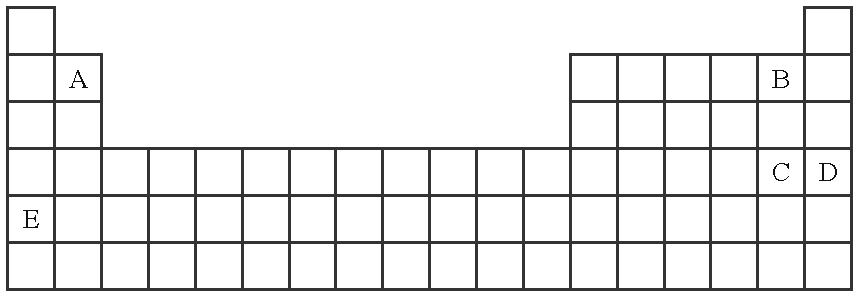
\includegraphics[width=0.6\linewidth]{FigurasSVG/UD2_Tabla_Periodica/pdf/UD2_E01_ejercicio_tabla.pdf}
        \caption{Tabla periódica}
        \label{fig:ejercicio_2}
    \end{figure}
    \begin{solu}
%        \begin{figure}[H]
%            \centering
%            \includegraphics[scale=.5]{ images/imagesUD2TablaPeriodica/UD2_Problemas/evauclm3a.png}
%            \includegraphics[scale=.5]{ images/imagesUD2TablaPeriodica/UD2_Problemas/evauclm3b.png}
%        \end{figure}

        Según su posición en el esquema de la tabla periódica: \(A\) está en el grupo 2, período 2 (berilio, \(Z=4\)); \(B\) está en el grupo 17, período 2 (flúor, \(Z=9\)); \(C\) y \(D\) están al final del período 3, en los grupos 17 y 18 respectivamente (cloro, \(Z=17\), y argón, \(Z=18\)); y \(E\) está en el grupo 1, período 4 (potasio, \(Z=19\)).

        \textbf{Configuraciones electrónicas}

        \begin{itemize}
            \item \(A\) (Be, \(Z=4\)): \(1s^2\,2s^2\)
            \item \(B\) (F, \(Z=9\)): \(1s^2\,2s^2\,2p^5\)
            \item \(C\) (Cl, \(Z=17\)): \(1s^2\,2s^2\,2p^6\,3s^2\,3p^5\)
            \item \(D\) (Ar, \(Z=18\)): \(1s^2\,2s^2\,2p^6\,3s^2\,3p^6\)
            \item \(E\) (K, \(Z=19\)): \(1s^2\,2s^2\,2p^6\,3s^2\,3p^6\,4s^1\)
        \end{itemize}

        Véase el ejercicio siguiente para el análisis razonado de las afirmaciones sobre estos elementos.

    \end{solu}

\end{exerciseEVAU}

\begin{exerciseEVAU}
    \textbf{2018 (continuación)}. Los elementos A, B, C, D y E son los mismos del ejercicio anterior, situados en el esquema de tabla periódica: \(A\) = Be (\(Z=4\)), \(B\) = F (\(Z=9\)), \(C\) = Cl (\(Z=17\)), \(D\) = Ar (\(Z=18\)) y \(E\) = K (\(Z=19\)).
    \begin{enumerate}[label=\letraminuscula]
    \item Escribe las configuraciones electrónicas de dichos elementos.
    \item Basándote en ellas justifica si son o no ciertas las siguientes afirmaciones:
    \begin{enumerate}
        \item La primera energía de ionización de E es mayor que la de A
        \item D es un gas noble y E un metal alcalinotérreo.
        \item La afinidad electrónica de B es mayor que la de A.
        \item El radio atómico de C es mayor que el de B.
    \end{enumerate}
    \end{enumerate}

    \begin{solu}

        \textbf{a) Configuraciones electrónicas}

        \begin{itemize}
            \item \(A\) (Be, \(Z=4\)): \(1s^2\,2s^2\)
            \item \(B\) (F, \(Z=9\)): \(1s^2\,2s^2\,2p^5\)
            \item \(C\) (Cl, \(Z=17\)): \(1s^2\,2s^2\,2p^6\,3s^2\,3p^5\)
            \item \(D\) (Ar, \(Z=18\)): \(1s^2\,2s^2\,2p^6\,3s^2\,3p^6\)
            \item \(E\) (K, \(Z=19\)): \(1s^2\,2s^2\,2p^6\,3s^2\,3p^6\,4s^1\)
        \end{itemize}

        \textbf{b) Análisis de las afirmaciones}

        \textbf{b.1) «La primera energía de ionización de E es mayor que la de A»: FALSO.}

        \(E\) (K) es un metal alcalino del grupo 1, con un único electrón de valencia muy alejado del núcleo (período 4), por lo que su energía de ionización es muy baja. \(A\) (Be) pertenece al grupo 2, con mayor carga nuclear efectiva sobre sus electrones de valencia y en una capa más interna (período 2), lo que le confiere una energía de ionización considerablemente mayor que la de \(E\).

        \textbf{b.2) «D es un gas noble y E un metal alcalinotérreo»: FALSO.}

        \(D\) (Ar) sí es un gas noble (grupo 18), pero \(E\) (K) tiene configuración \(4s^1\), propia de un \textbf{metal alcalino} (grupo 1), no de un metal alcalinotérreo (grupo 2, que tendría configuración \(ns^2\)). Por tanto, la primera parte es cierta, pero la segunda es falsa.

        \textbf{b.3) «La afinidad electrónica de B es mayor que la de A»: VERDADERO.}

        \(B\) (F) tiene mayor carga nuclear (\(Z=9\)) que \(A\) (Be, \(Z=4\)) y, al pertenecer ambos al período 2 con un apantillamiento interno similar, también mayor carga nuclear efectiva \(Z_{ef}\) sobre su capa de valencia. \(B\) es además un halógeno al que solo le falta un electrón para alcanzar la configuración de gas noble, por lo que su afinidad electrónica es muy alta (proceso muy favorable). \(A\) (Be), en cambio, tiene la subcapa \(2s\) completa, una configuración de especial estabilidad que dificulta la entrada de un electrón adicional; su afinidad electrónica es prácticamente nula o incluso desfavorable. Por tanto, la afinidad electrónica de \(B\) es, efectivamente, mayor que la de \(A\).

        \textbf{b.4) «El radio atómico de C es mayor que el de B»: VERDADERO.}

        \(C\) (Cl) y \(B\) (F) pertenecen al mismo grupo (17), pero \(C\) se encuentra en el período 3 y \(B\) en el período 2. Al descender en un grupo, el radio atómico aumenta porque los electrones de valencia ocupan capas cada vez más alejadas del núcleo. Por tanto, el radio de \(C\) es mayor que el de \(B\).

    \end{solu}
\end{exerciseEVAU}

\begin{exerciseEVAU}
    \textbf{2021}.
    A partir de los átomos A (Z =19) y B (Z = 35): a) Escriba sus configuraciones electrónicas, indique el grupo y el periodo al que pertenecen. b) ¿El radio del ion más estable de A es inferior al del ion más estable de B? Justifíquelo. c) ¿Qué se entiende por primera energía de ioniza ión de un átomo? ¿Cuál de los átomos A y B tendría mayor energía de ionización? d) Formule el compuesto binario que podrían formar A y B razonando el tipo de enlace que se generaría.

    \begin{solu}
%        \begin{figure}[H]
%            \centering
%            \includegraphics[scale=.5]{ images/imagesUD2TablaPeriodica/UD2_Problemas/evauclm4.png}
%        \end{figure}

        \textbf{a) Configuraciones electrónicas, grupo y período}

        \begin{itemize}
            \item \(A\) (\(Z=19\), K): \(1s^2\,2s^2\,2p^6\,3s^2\,3p^6\,4s^1\) — grupo 1, período 4.
            \item \(B\) (\(Z=35\), Br): \(1s^2\,2s^2\,2p^6\,3s^2\,3p^6\,4s^2\,3d^{10}\,4p^5\) — grupo 17, período 4.
        \end{itemize}

        \textbf{b) Comparación de los radios iónicos}

        El ion más estable de \(A\) es \(\ch{K+}\) (pierde su único electrón de valencia y adquiere la configuración del \ch{Ar}, con capa de valencia \(n=3\)). El ion más estable de \(B\) es \(\ch{Br-}\) (gana un electrón y adquiere la configuración del \ch{Kr}, con capa de valencia \(n=4\)).

        Como \(\ch{Br-}\) tiene su capa de valencia en \(n=4\) (más externa) y muchos más electrones que \(\ch{K+}\) (36 frente a 18), su radio es considerablemente mayor: la mayor extensión de la nube electrónica prevalece sobre el hecho de que la carga nuclear de \(\ch{Br-}\) (\(Z=35\)) sea mayor que la de \(\ch{K+}\) (\(Z=19\)). Por tanto, \textbf{sí}, el radio de \(\ch{K+}\) es inferior al de \(\ch{Br-}\).

        \textbf{c) Primera energía de ionización}

        La primera energía de ionización es la energía necesaria para arrancar el electrón más externo (el menos retenido) a un átomo aislado en estado fundamental y gaseoso, dando lugar a un catión monopositivo.

        Entre \(A\) y \(B\), el bromo (\(B\)) tiene mayor carga nuclear (\(Z=35\)) y, al ser un no metal próximo a la configuración de gas noble, una elevada carga nuclear efectiva \(Z_{ef}\) sobre sus electrones de valencia, por lo que los retiene con mucha más fuerza que el potasio (\(A\)), un metal alcalino con un único electrón de valencia muy alejado del núcleo y muy apantallado (\(Z_{ef}\) baja). Por tanto, \(\boldsymbol{B}\) \textbf{(Br) tiene mayor energía de ionización}.

        \textbf{d) Compuesto binario entre A y B}

        El potasio (metal muy electropositivo) cede su electrón de valencia al bromo (no metal muy electronegativo), formando el compuesto iónico:

        \begin{equation*}
            \ch{KBr}
        \end{equation*}

        (bromuro de potasio), unido mediante \textbf{enlace iónico}.

    \end{solu}
\end{exerciseEVAU}


\begin{exerciseEVAU}
    \textbf{2017}. Los átomos neutros A, B, C y D tienen las siguientes configuraciones electrónicas: $A = 1s^2 2s^2 2p^1$; $B = 1s^2 2s^2 2p^5$; $C = 1s^2 2s^2 2p^6 3s^2$; $D = 1s^2 2s^2 2p^6$
    a) Indica el grupo y período en el que se encuentran.
    b) El nombre y símbolo de cada elemento
    c) Ordena razonadamente, de mayor a menor electronegatividad.
    d) ¿Cuál de ellos presentará mayor potencial de ionización?

    \begin{solu}
%        \begin{figure}[H]
%            \centering
%            \includegraphics[scale=.5]{ images/imagesUD2TablaPeriodica/UD2_Problemas/evauclm3a.png}
%        \end{figure}

        A partir de las configuraciones electrónicas dadas, identificamos cada elemento: \(A\) tiene 5 electrones (\(Z=5\), boro), \(B\) tiene 9 electrones (\(Z=9\), flúor), \(C\) tiene 12 electrones (\(Z=12\), magnesio) y \(D\) tiene 10 electrones (\(Z=10\), neón).

        \textbf{a) Grupo y período}

        \begin{itemize}
            \item \(A\) (B, \(Z=5\)): grupo 13, período 2.
            \item \(B\) (F, \(Z=9\)): grupo 17, período 2.
            \item \(C\) (Mg, \(Z=12\)): grupo 2, período 3.
            \item \(D\) (Ne, \(Z=10\)): grupo 18, período 2.
        \end{itemize}

        \textbf{b) Nombre y símbolo}

        \(A\) = boro (\ch{B}); \(B\) = flúor (\ch{F}); \(C\) = magnesio (\ch{Mg}); \(D\) = neón (\ch{Ne}).

        \textbf{c) Orden de mayor a menor electronegatividad}

        El flúor es el elemento más electronegativo de toda la tabla periódica. El magnesio, al ser un metal, tiene una electronegatividad baja. El neón, al ser un gas noble prácticamente inerte, no forma enlaces en condiciones normales y carece de un valor de electronegatividad de Pauling definido (o se considera nulo a estos efectos). Entre los elementos con electronegatividad definida:

        \begin{equation*}
            B\,(\ch{F}) > A\,(\ch{B}) > C\,(\ch{Mg})
        \end{equation*}

        \textbf{d) Elemento con mayor potencial de ionización}

        Los cuatro elementos pertenecen al período 2, por lo que el apantallamiento interno es similar para todos ellos y la carga nuclear efectiva \(Z_{ef} = Z - \sigma\) aumenta con el número atómico: \(D\) (Ne, \(Z=10\)) tiene la mayor \(Z_{ef}\) del grupo. \(D\) (neón) presenta el mayor potencial de ionización, ya que posee configuración de capa cerrada (gas noble), de especial estabilidad, lo que, junto con su elevada carga nuclear efectiva, dificulta enormemente arrancarle un electrón.

    \end{solu}
\end{exerciseEVAU}





    \chapter{Enlace Químico}

    \section{Concepto de enlace químico}\label{sec:concepto-de-enlace-quimico}

    \begin{definition}[Enlace Químico]
        El \textbf{enlace químico} es el conjunto de fuerzas que mantienen unidos los átomos cuando forman moléculas o cristales, así como las fuerzas que mantienen unidas las moléculas cuando se presentan en estado sólido o líquido.
    \end{definition}

Los tres enlaces que conocemos son: \textbf{enlace iónico}, \textbf{enlace covalente} y \textbf{enlace metálico}.

%    \subsection{Teorías del enlace químico}
%
%    Para explicar la formación de estos enlaces, se han ido estableciendo diferentes teorías de las que podemos destacar:
%
%    \begin{enumerate}[label=\numberballmDarkTeal]
%        \item \negrita{Teoria de Lewis}: los átomos se unen con otros átomos ganando, perdiendo o compartiendo electrones de las capas externas, en un número que les permita conseguir la configuración de gas noble.
%        A esta teoría se le conoce como \blueremark{regla del octeto}.
%        Esta teoría es acertada para el enlace iónico pero no para muchos aspectos del enlace covalente y por eso se propusieron otras teorías.
%        \item \negrita{Teoría del enlace de valencia}: trata la formación del enlace covalente desde un punto de vista del apareamiento de los espines electrónicos y del máximo solapamiento de los orbitales atómicos.
%        \item \negrita{Teoría de los orbitales moleculares}: considera la molécula como un conjunto y explica cómo situar los electrones en una serie de orbitales moleculares, del mismo modo que se colocan los electrones en los átomos en los correspondientes orbitales atómicos.
%    \end{enumerate}


\section{Enlace iónico}\label{sec:enlace-ionico}


    \begin{definition}[Enlace iónico]
        El \textbf{enlace iónico} se establece cuando se combinan elementos con electronegatividades muy diferentes:
        \begin{itemize}
            \item El más electronegativo (no metal) formará iones negativos y el menos electronegativo (metal), iones positivos.
            \item El enlace se produce por atracción electrostática entre iones que tienen carga de distinto signo.
        \end{itemize}
    \end{definition}


Normalmente, los enlaces iónicos se forman entre halógenos (grupo 17) y algún alcalino (grupo 1, a excepción del hidrógeno) o alcalinotérreo (grupo 2).

Una característica fundamental de los compuestos con enlace iónico es que forman redes cristalinas donde los iones de un signo están rodeados por los de signo contrario.

\begin{figure}[H]
    \centering
    % [FIGURA ORIGINAL] \includegraphics[scale=0.8]{images/imagesUD3EnlaceQuimico/UD3_Teoria/redes_cristalinas}
    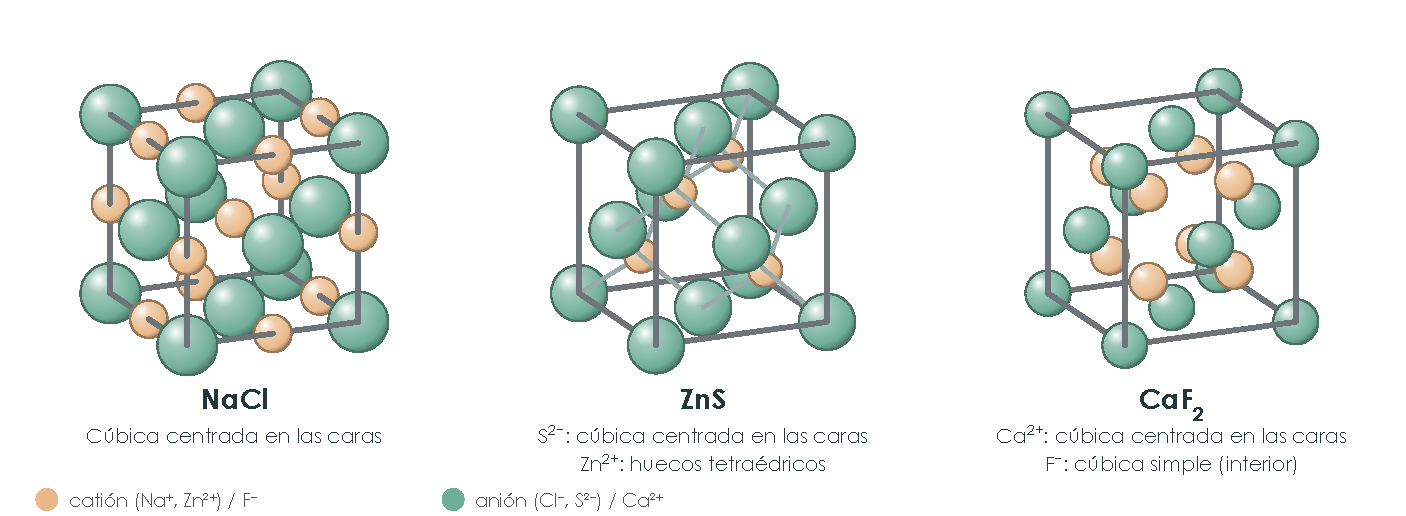
\includegraphics[width=0.95\linewidth]{FigurasSVG/UD3_Enlace_Quimico/pdf/UD3_01_redes_cristalinas.pdf}
    \caption{Redes cristalinas}
    \label{fig:redes_cristalinas}
\end{figure}

%    La descripción geométrica de estas agrupaciones de iones se hacen en función del:
%
%    \begin{enumerate}
%        \item Tipo de \blueremark{malla} u ordenación regular que adoptan.
%        \item \negrita{Número} ó \negrita{índice de coordinación}, siendo el número de iones de signo contrario que envuelven a un ion de signo contrario.
%    \end{enumerate}

% \begin{figure}[H]
%     \centering
%     \includegraphics[scale=0.45]{images/imagesUD3EnlaceQuimico/UD3_Teoria/redes_ionicas_tabla}
%     \caption{Tipos de principales redes iónicas y ejemplos de compuestos}
%     \label{fig:tipos_redes_ionicas}
% \end{figure}

\subsection{Teoría de Lewis sobre el enlace iónico}\label{subsec:teoria-de-lewis-sobre-el-enlace-ionico}

Según la teoría de Lewis, el enlace iónico es el proceso por el cual los átomos ganan, ceden o comparten electrones de las capas externas hasta conseguir la configuración de un gas noble.

Es importante introducir la \blueremark{estructura de Lewis} como aquella representación de los electrones del último nivel o capa de un átomo, ion o molécula, mediante puntos, círculos, cruces, rayas \dots

A continuación vemos la estructura de Lewis para algunos átomos neutros

\begin{figure}[H]
    \centering
    % [FIGURA ORIGINAL] \includegraphics[scale=0.45]{images/imagesUD3EnlaceQuimico/UD3_Teoria/lewis_atomos_neustros}
    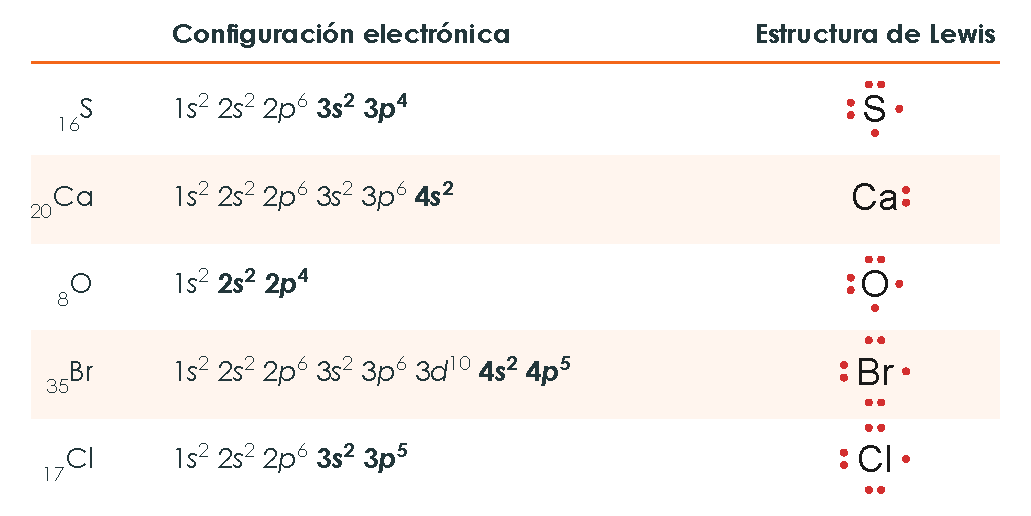
\includegraphics[width=0.8\linewidth]{FigurasSVG/UD3_Enlace_Quimico/pdf/UD3_02_lewis_atomos_neutros.pdf}
    \caption{Estructura de Lewis para átomos neutros}
    \label{fig:lewis_newtros}
\end{figure}

En el momento de la formación de un enlace iónico, se forman cationes y aniones, quedando, por tanto, su estructura de Lewis de la siguiente forma:

\begin{figure}[H]
    \centering
    % [FIGURA ORIGINAL] \includegraphics[scale=.45]{images/imagesUD3EnlaceQuimico/UD3_Teoria/lewis_iones}
    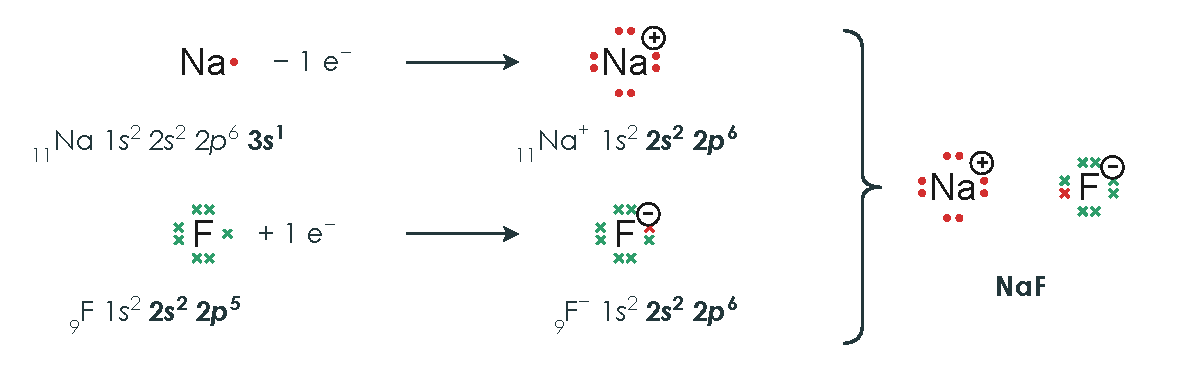
\includegraphics[width=0.85\linewidth]{FigurasSVG/UD3_Enlace_Quimico/pdf/UD3_03_lewis_iones.pdf}
    \caption{Estructura de Lewis para iones}
    \label{fig:lewis_iones}
\end{figure}

\subsection{Energía reticular \texorpdfstring{$\bm{U}$}{U}. Balance energético de la formación de un cristal iónico}\label{subsec:energia-reticular-texorpdfstring{$bm{u}$}{u}.-balance-energetico-de-la-formacion-de-un-cristal-ionico}

La \blueremark{energía reticular} (\(\bm{U}\)) la podemos definir de tres maneras diferentes:


    \begin{enumerate}[label=\letraminuscula]
            \item La energía necesaria para separar los iones que forman una red cristalina hasta una distancia infinita.
            En este caso la energía será positiva.
            \item \textbf{La energía que se desprende cuando dos iones en estado gaseoso se aproximan para formar un compuesto iónico. En este caso la energía será negativa.}
            \item La energía que hay que comunicar a un mol de un compuesto iónico para que sus iones se separen a una distancia que dejen de interaccionar.
            En este caso la energía será positiva.
    \end{enumerate}

La energía reticular nos determinará:
\begin{enumerate}[label=\letraminuscula]
        \item Estabilidad.
        \item Solubilidad.
        \item Dureza.
\end{enumerate}

\subsection{Cálculo de la energía reticular}\label{subsec:calculo-de-la-energia-reticular}

La energía reticular la podemos calcular de manera experimental utilizando el ciclo de Born-Haber o de manera teórica usando la ecuación de Born-Landé.

\begin{enumerate}[label=\numberballmDarkTeal]
        \item \negrita{Ciclo de Born-Haber}.
        El ciclo de \textbf{Born-Haber} es un ciclo termodinámico en que se estudian, desde el punto de vista energético, todos los procesos que intervienen en la formación de un mol de un compuesto iónico a partir de las sustancias simples que lo integran cuando se encuentran en su estado termodinámico más estable.

        Como ejemplo veremos la formación del \ch{NaCl \sld{}} a partir de \ch{Na \sld{}} y \ch{Cl2 \gas{}} en su estado más estable.

        La energía del proceso se llama \textbf{entalpía de formación} del \ch{NaCl}, \(\Delta H_f\).

        \begin{equation*}
            \ch{Na \sld{} + 1/2 Cl2 \gas{} -> NaCl \sld{}} \qquad \qquad \Delta H_f = \energia[kjmol]{-411} \rightarrow \text{1 mol serán } \energia[kj]{-411}
        \end{equation*}

        Este paso global, lo podemos dividir en otros más sencillos o elementales:

        \begin{enumerate}[label=\numberballmDarkTeal]
            \item Sublimación del \ch{Na \sld{}} a \ch{Na \gas{}} para obtener los átomos de sodio aislados:
            \begin{equation*}
                \ch{Na \sld{}  -> Na \gas{}} \qquad  \Delta H_{sub} = \energia[kjmol]{107.3} \rightarrow \text{1 mol serán } \energia[kj]{107.3}
            \end{equation*}

            \item Disociación de las moléculas de \ch{Cl2 \gas{}} para obtener átomos de \ch{Cl} aislados, en este proceso tenemos que disociar \(\dfrac{1}{2}\) mol de moléculas de cloro:

            \begin{equation*}
                \ch{1/2 Cl2 \gas{}  -> Cl \gas{}} \qquad   \Delta H_{dis} = \energia[kjmol]{244} \rightarrow \dfrac{1}{2} \text{mol} \cdot 244 \unit{\kilo\joule\per\mole} =  \energia[kj]{122}
            \end{equation*}

            \item Ionización del \ch{Na \gas{}} a \ch{Na+ \gas{}} y para ello habrá que administrar la energía equivalente a la primera energía o potencial de ionización del sodio:

            \begin{equation*}
                \ch{Na \gas{}  -> Na+ \gas{}} \qquad   EI = \energia[kjmol]{495.8} \rightarrow  \text{1 mol serán }  \energia[kj]{495.8}
            \end{equation*}

            \item Ionización del \ch{Cl \gas{}} a \ch{Cl- \gas{}} en la que se desprenderá una energía equivalente a la primera afinidad electrónica del cloro:

            \begin{equation*}
                \ch{Cl \gas{}  -> Cl- \gas{}} \qquad   AE = \energia[kjmol]{-348.6} \rightarrow  \text{1 mol serán }  \energia[kj]{-348.6}
            \end{equation*}
            \item Energía reticular \(\bm{U}\), es la energía que se desprende al formar un mol de \ch{NaCl \sld{}} a partir de los iones constituyentes del estado gaseoso:

            \begin{equation*}
                \ch{Na+ \gas{} + Cl- \gas{} -> NaCl \sld{}} \qquad  \Delta U_r = \energia[kjmol]{-787} \rightarrow \text{1 mol serán } \energia[kj]{-787}
            \end{equation*}

        \end{enumerate}

        Si aplicamos la Ley de Hess (el cambio de energía requerido en una reacción entre reactivos para dar productos es el mismo independientemente de que si la reacción se efectúe en un paso o en una serie de pasos):

        \begin{equation}
            \Delta H_{f} = \Delta H_{sub} + EI + \dfrac{1}{2} \Delta H_{dis} + AE + {\color {red} U_r}
        \end{equation}

        Si lo que queremos es obtener el valor de la energía reticular, basta con despejar y obtendremos:
        \begin{equation}
            {\color {red} U_r}
            = \Delta H_{f} - \Delta H_{sub} - EI - \dfrac{1}{2} \Delta H_{dis} - AE
        \end{equation}

        A continuación, se muestra un esquema del proceso:

        %   El \ch{NaCl} lo podemos formar a partir de sodio sólido y cloro molecular en estado gaseoso. Si mezclamos ambos reactivos no dará el \ch{NaCl} en estado sólido requiriéndose o desprendiéndose una determinada energía a la que llamamos entalpía de formación ($\Delta H_f$).

        \begin{figure}[H]
            \centering
            % [FIGURA ORIGINAL] \includegraphics[scale=1]{images/imagesUD3EnlaceQuimico/UD3_Teoria/cicloborhhabberNaCl}
            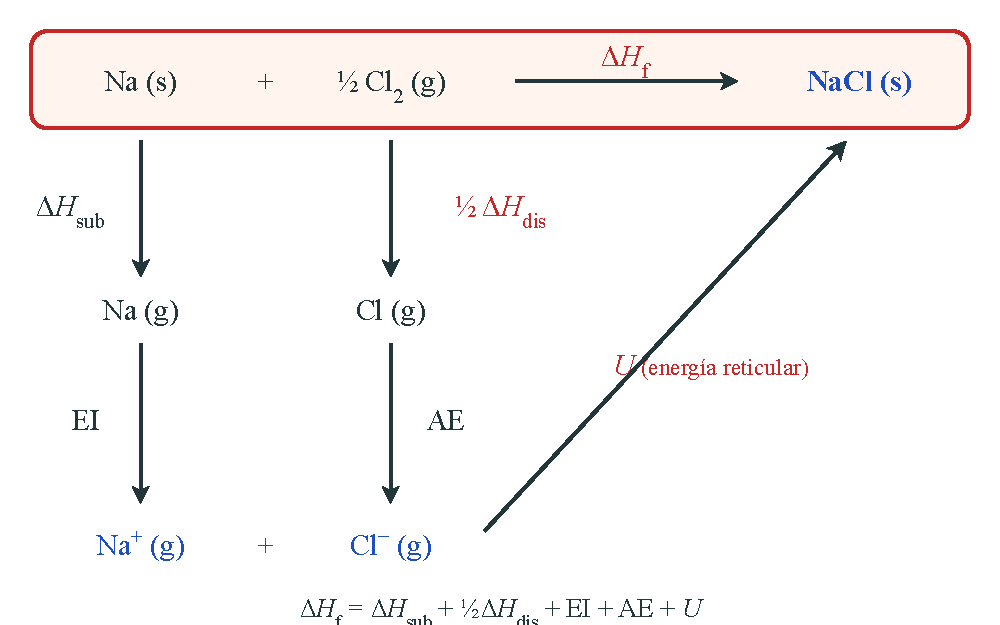
\includegraphics[width=0.75\linewidth]{FigurasSVG/UD3_Enlace_Quimico/pdf/UD3_04_ciclo_born_haber_NaCl.pdf}
            \caption{Ciclo de Born-Haber para el NaCl}
        \end{figure}

        \item \negrita{Ecuación de Born-Landé}
        \begin{equation}
            U_r = -\; N_A\ K\ \dfrac{Q_{\text{anión}}\ Q_{\text{catión}}}{d_0}\; A\ \left(1 - \dfrac{1}{n} \right)
            \label{eq:ecuacion_born_lande}
        \end{equation}

        Siendo:
        \begin{gather*}
            K = \text{Constante de Coulomb} = \dfrac{1}{4\pi\varepsilon_0} = \SI{9e9}{\N\square\metre\per\square \coulomb} (\text{en el vacío})\\
            Q_{\text{catión}} = \text{Carga del catión en Culombios}\\
            Q_{\text{anión}} = \text{Carga del anión en Culombios} \\
            A = \text{Constante de Madelung} \\
            d_0 = \text{distancia entre iones} = r_{\text{anión}} + r_{\text{catión}}\\
            n = \text{factor de Born}
        \end{gather*}
        A efectos prácticos, la \( Q_{\text{catión}} \) y \( Q_{\text{anión}} \) se le asignará el estado de oxidación de dicho ión.
%        Para calcular la carga tanto del anión como del catión sería: \(Q = | \text{carga de la especie} | \cdot | q_{\el} |\) siendo \(q_{\el} = \text{carga del electrón} = \SI{-1.6e-19}{\coulomb} \)
\end{enumerate}
El factor de Born es propio de cada par de iones.

La constante de Madelung es una constante que depende del tipo de red cristalina que forma el compuesto iónico.
%    ,siendo sus principales valores:
%
%    \begin{figure}[H]
%        \centering
%        \includegraphics[scale=0.45]{images/imagesUD3EnlaceQuimico/UD3_Teoria/valores_cte_madelung}
%        \caption{Valores de la constante de Madelung para algunas celdas iónicas}
%        \label{fig:constantedemadelungvalores}
%    \end{figure}

%    Para obtener el valor del factor de Born o compresibilidad que depende de la configuración electrónica de los iones, tenemos que conocer la siguiente tabla:
%
%
%    \begin{figure}[H]
%        \centering
%        \includegraphics[scale=.45]{images/imagesUD3EnlaceQuimico/UD3_Teoria/factor_de_born}
%        \caption{Factor de Born}
%        \label{fig:factor_born}
%    \end{figure}
%
%    Para conocer el valor del factor de Born para cada ión, tenemos que ver que configuración electronica adquiere cuando gana o pierde electrones. Luego determinamos que gas noble tiene la configuración electrónica adoptada y le asignamos a ese ión el valor que tenemos en la tabla anterior. Para conocer el valor total del compuesto iónico se hace la media aritmética de ambos factores de Born asignados a cada ión:
%
%
%    \begin{equation}
%        n_{\text{iónico}} = \dfrac{(n_{\text{anion}} + n_{\text{cation}})}{2}
%    \end{equation}
%
%    Por ejemplo, para determinar el el factor de Born par el \ch{NaCl}:
%
%    \begin{enumerate}[label=\numberballred]
%        \item \ch{Na}: \rojo{\elconf{11}} \ch{->} \ch{Na^+} quedando \azul{\elconf{10}} quedando la configuración de \negrita{\textcolor{mygreen}{\elementsymbol{10}}} quedando $n_{cation} = 7$.
%        \item \ch{Cl}: \rojo{\elconf{17}} \ch{->} \ch{Cl^-} quedando \azul{\elconf{18}} quedando la configuración de \negrita{\textcolor{mygreen}{\elementsymbol{18}}} quedando $n_{anion} = 9$.
%        \item Por lo tanto, el factor del Born para el \ch{NaCl} será:
%        \begin{equation*}
%            n_{NaCl} = \dfrac{7 + 9}{2} = 8
%        \end{equation*}
%    \end{enumerate}

\subsection{Propiedades de los compuestos iónicos}

Las propiedades de los compuestos iónicos, se derivan de su propia \blueremark{estructura} y de su naturaleza \blueremark{electrostática} del enlace entre los iones.

Entre sus propiedades podemos destacar:

\begin{enumerate}[label=\numberballmDarkTeal]
        \item A temperatura ambiente, los compuestos iónicos son \negrita{\azul{sólidos cristalinos}}.
        \item Tienen elevados puntos de fusión y ebullición, debido a que hay que administrar mucha energía para destruir la estructura cristalina.
        \item A mayor ($\uparrow$) energía reticular mayor punto de fusión ($\uparrow$).
        \item No conducen la electricidad en estado sólido pero \negrita{\rojo{SI}} cuando están fundidos o en disolución, debido a la movilidad de sus iones.
        \item Son duros, a mayor energía reticular mayor dureza.
        \item Son frágiles y poco flexibles.
        \item Son solubles en disolventes polares, como el agua.
        Las moléculas de agua se van colocando alrededor de la estructura cristalina hasta que consigue romperla impidiendo que vuelvan a unirse.
        A la energía implicada en este proceso se le conoce como \azuln{energía de solvatación}
        \item Si la energía de solvatación es negativa y en valor absoluto superior a la \verden{energía reticular} la disolución será un proceso \verden{exotérmico} produciéndose así un aumento en la temperatura.
\end{enumerate}


\section{Enlace covalente}

El enlace covalente se da entre dos \azuln{no metales} o elementos del bloque \verden{p} de la tabla periódica.
La diferencia de electronegatividad no debe ser superior a 1.

El enlace covalente se da normalmente entre elementos de los grupos 13 al 17 incluido el hidrógeno.

\subsection{Teoría de Lewis del enlace covalente}

Un \azuln{enlace covalente} se forma cuando dos átomos \azuln{comparten} un par de electrones. Por ejemplo:
    \begin{center}
        \lewis{H}{}{}{}{}{.}{}{}{} + \lewis{H}{}{.}{}{}{}{}{}{} \ch{->} \lewis{H}{}{}{}{}{}{}{}{}\hspace{-0.5em}---\hspace{-0.75em}\lewis{H}{}{}{}{}{}{}{}{}
    \end{center}


Lewis pensó que los gases nobles tenían la configuración más estable posible, ya que no formaban compuestos y, por tanto, los demás elementos hacían todo lo posible por adquirir una configuración de gas noble que le diera estabilidad.
Al tener los gases nobles ocho electrones en su última capa (a excepción del \ch{He}) se le llamó  \azuln{regla del octeto}.
Esto se demuestra con la formación de \ch{F2}.

%    \begin{figure}[H]
%        \centering
%        \includegraphics[scale=1]{images/imagesUD3EnlaceQuimico/UD3_Teoria/formacionf2_lewis}
%        \caption{Formación de \ch{F2}. Estructura de Lewis}
%        \label{fig:f2_covalente}
%    \end{figure}

\begin{figure}[H]
    \centering
    % [FIGURA ORIGINAL] \includegraphics[scale=0.5]{images/imagesUD3EnlaceQuimico/UD3_Teoria/lewis_F2}
    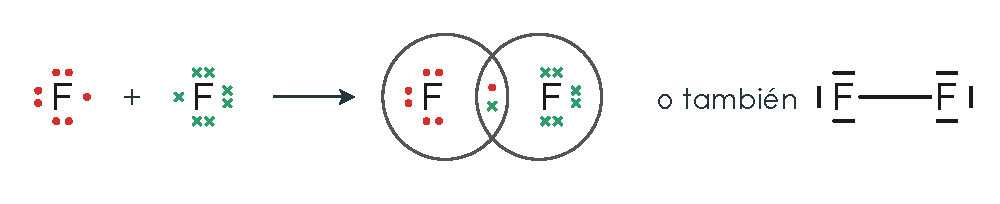
\includegraphics[width=0.7\linewidth]{FigurasSVG/UD3_Enlace_Quimico/pdf/UD3_05_formacion_F2_lewis.pdf}
    \caption{Formación de \ch{F2}. Estructura de Lewis}
    \label{fig:f2_covalente}
\end{figure}
Algo similar tendremos para el agua, amoniaco o nitrógeno
\begin{figure}[H]
    \centering
    % [FIGURA ORIGINAL] \includegraphics[scale=0.5]{images/imagesUD3EnlaceQuimico/UD3_Teoria/lewis_agua_amoniaco_nitrogeno}
    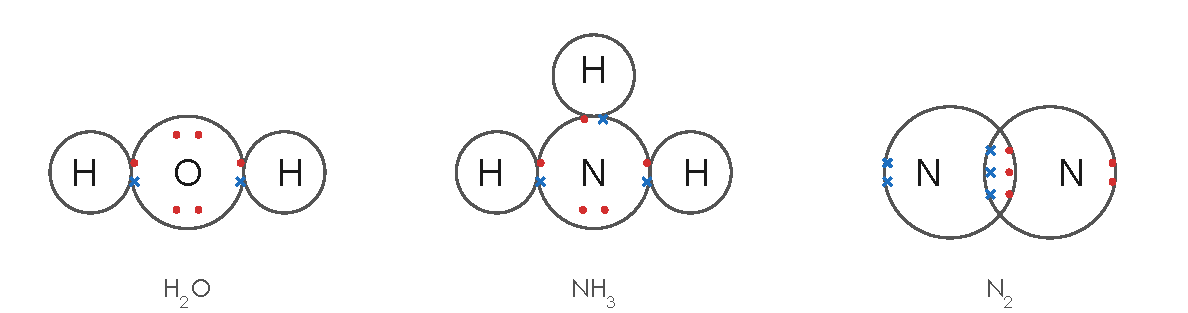
\includegraphics[width=0.85\linewidth]{FigurasSVG/UD3_Enlace_Quimico/pdf/UD3_06_lewis_agua_amoniaco_nitrogeno.pdf}
    \caption{Formación agua, amoniaco y nitrógeno}
    \label{fig:agua_amoniaco_nitrogeno}
\end{figure}

Algunas veces los átomos pueden alcanzar su octeto compartiendo dos o tres pares de electrones para formar así un doble o un triple enlace (ver Figura~\ref{fig:estructuras_lewis} más adelante)

Llamamos \azuln{orden de enlace} al número de pares de electrones compartidos en una molécula.

\subsection{Reglas para escribir estructuras de Lewis}
Para escribir correctamente las estructuras de Lewis podemos seguir los siguientes pasos (tomaremos como ejemplo la formación de \ch{F2}):

\begin{enumerate}[label=\numberballmDarkTeal]
        \item Sumar los electrones de valencia de los átomos $7 + 7 = 14$ \elec.
        Los llamaremos electrones de valencia (EV).

        \item Calculamos los pares de electrones de valencia (PEV) según $\dfrac{\text{electrones de valencia}}{2}$.Para el \ch{F2} tendremos $\dfrac{14}{2} = 7$.

        \item Contar los electrones que necesitaríamos para que todos los átomos completaran la configuración de gas noble, es decir completaran el octeto a excepción del hidrógeno que le contabilizaríamos 2 electrones. $8 \times 2 = 16$ \elec.
        Los llamaremos electrones del octeto.

        \item Calculamos los pares de electrones enlazantes (PE) según:
        \begin{equation}
            PE = \dfrac{\text{electrones del octeto} - \text{electrones de valencia}}{2}
        \end{equation}
        En el caso del \ch{F2} tendremos que: $\dfrac{16 - 14}{2} = 1$
        \item Ahora calculamos los pares de electrones no enlazantes (PEN) según:
        \begin{equation}
            PEN = PEV - PE
        \end{equation}
        En el caso del \ch{F2} tendremos que: $PEN = 7 - 1 = 6$
        \item Situamos ahora los átomos poniendo el átomo central aquel que sea menos electronegativo a excepción del hidrógeno que nunca se pondrá en el centro.

        \item Ahora vamos colocando los pares de electrones enlazantes (son los que enlazan a otros átomos) y no enlazantes (se sitúan alrededor de cada átomo) de manera que se vayan completando el octeto en todos los átomos
        \begin{figure}[H]
            \centering
            % [FIGURA ORIGINAL] \includegraphics[scale=1]{images/imagesUD3EnlaceQuimico/UD3_Teoria/F2_lewis}
            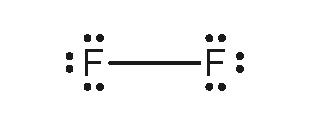
\includegraphics[width=0.22\linewidth]{FigurasSVG/UD3_Enlace_Quimico/pdf/UD3_07_F2_lewis.pdf}
            \caption{Estructura de Lewis para el \ch{F2}}
            \label{fig:fluor_lewis}
        \end{figure}
\end{enumerate}
A continuación se muestran más ejemplos de estructuras de Lewis:
\begin{figure}[H]
    \centering
    % [FIGURA ORIGINAL] \includegraphics[scale=1]{images/imagesUD3EnlaceQuimico/UD3_Teoria/lewis_varios}
    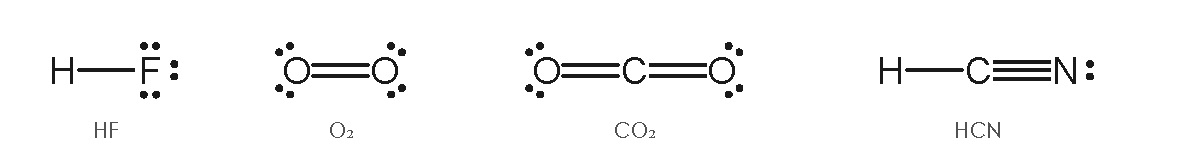
\includegraphics[width=0.8\linewidth]{FigurasSVG/UD3_Enlace_Quimico/pdf/UD3_08_lewis_varios.pdf}
    \caption{Estructuras de Lewis}
    \label{fig:estructuras_lewis}
\end{figure}

\subsection{Excepciones a la regla del octeto}

Podemos tener dos posibles casos, octetos incompletos y octetos ampliados.

\begin{enumerate}[label=\numberballmDarkTeal]
        \item \textbf{Octetos incompletos}: existen átomos que puede formar compuestos sin llegar a completar el octeto, son el caso del \blueremark{boro} y \blueremark{aluminio}.
        En estos casos, llegaran a tener 6 electrones en lugar de 8.
        \begin{figure}[H]
            \centering
            % [FIGURA ORIGINAL] \includegraphics[scale=1]{images/imagesUD3EnlaceQuimico/UD3_Teoria/octeto_incomleto}
            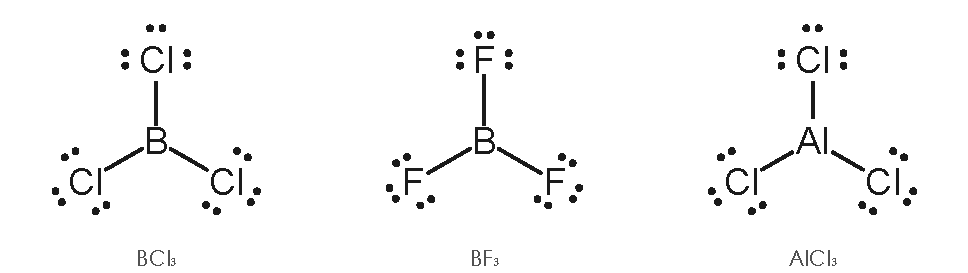
\includegraphics[width=0.7\linewidth]{FigurasSVG/UD3_Enlace_Quimico/pdf/UD3_09_octeto_incompleto.pdf}
            \caption{\ch{BCl3}, \ch{BF3} y \ch{AlCl3}}
            \label{fig:octetoincompleto}
        \end{figure}
        \item \textbf{Octeto ampliado}: a partir del tercer periodo, los elementos presentan orbitales $d$ vacíos y por lo tanto los átomos pueden ampliar su capa de valencia a 10, 12 o más electrones.
        Esto nos permite formar más enlaces de los previstos según la regla de Lewis, estos casos los encontramos principalmente en el \blueremark{azufre} y en el \blueremark{fósforo}.
        \begin{figure}[H]
            \centering
            % [FIGURA ORIGINAL] \includegraphics[scale=1]{images/imagesUD3EnlaceQuimico/UD3_Teoria/Lewis_Octeto_Ampliado}
            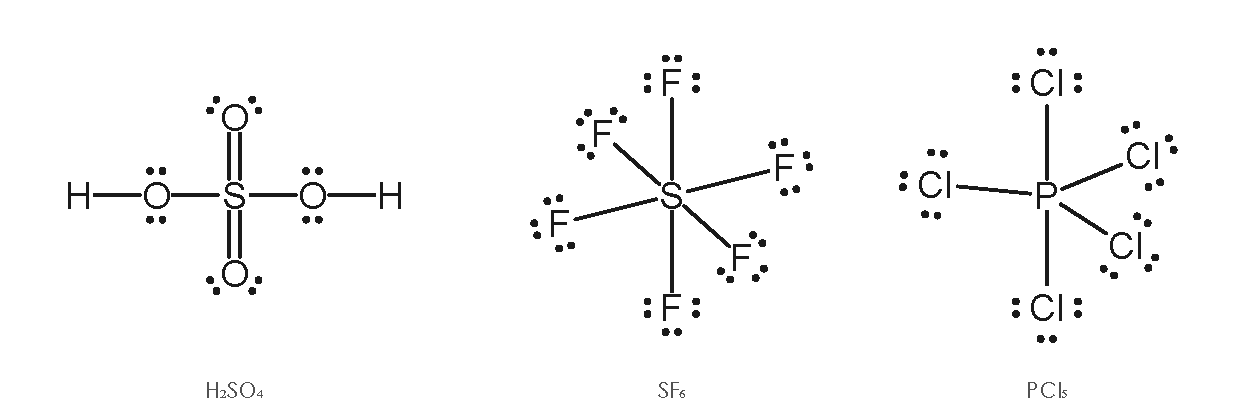
\includegraphics[width=0.8\linewidth]{FigurasSVG/UD3_Enlace_Quimico/pdf/UD3_10_octeto_ampliado.pdf}
            \caption{\ch{H2SO4}, \ch{SF6} y \ch{PCl5}}
            \label{fig:octetoampliado}
        \end{figure}
        \item \textbf{Moléculas con número impar de electrones}: se da cuando la suma de los electrones de valencia suman un número impar.
        En estos casos al menos uno de los átomos no conseguirá completar el octeto.
        Un ejemplo sería el \ch{NO}
        \begin{figure}[H]
            \centering
            % [FIGURA ORIGINAL] \includegraphics[scale=1]{images/imagesUD3EnlaceQuimico/UD3_Teoria/NO}
            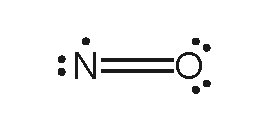
\includegraphics[width=0.18\linewidth]{FigurasSVG/UD3_Enlace_Quimico/pdf/UD3_11_NO_lewis.pdf}
            \caption{\ch{NO}}
            \label{fig:numeroimparelectrones}
        \end{figure}
\end{enumerate}

\marcador{Escribir las siguientes estructuras de Lewis}: \ch{H2SO3}, \ch{HNO3}, \ch{CH4}, \ch{CCl4}

\subsection{Resonancia}\label{subsec:resonancia}

En algunas ocasiones, podemos escribir más de una estructura de Lewis para un mismo compuesto.
Al conjunto de estas estructuras de Lewis se les denomina \negrita{estructuras resonantes}.

\begin{figure}[H]
    \centering
    % [FIGURA ORIGINAL] \includegraphics[scale=1]{images/imagesUD3EnlaceQuimico/UD3_Teoria/estructuras_resonantes_NO3}
    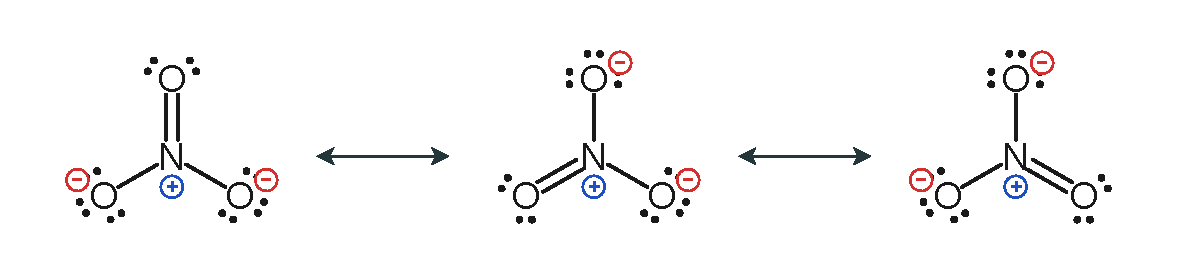
\includegraphics[width=0.85\linewidth]{FigurasSVG/UD3_Enlace_Quimico/pdf/UD3_12_resonancia_NO3.pdf}
    \caption{Estructuras resonantes de ión nitrato \ch{NO3-}}
    %\label{fig:}
\end{figure}

Aunque podamos escribir varias estructuras resonantes, siempre habrá una que contribuya más y sea la mayoritaria.
%    y para ello podemos seguir las siguientes reglas:
%    \begin{enumerate}[label=\numberballmDarkTeal]
%        \item Las estructuras resonantes sólo suponen movimiento de electrones desde posiciones adyacentes (nunca de átomos).
%        El movimiento de electrones se representan con flechas.
%        \item Las estructuras resonantes en las que los átomos del segundo periodo poseen octetos completos son más importantes que las que tienen octetos incompletos.
%        \item Las estructuras más importantes son aquellas que supongan la \negrita{mínima separación de cargas}.
%        Se debe intentar no tener cargas en los átomos.
%        \item En los casos en que una estructura de Lewis con octetes completos no puede representarse sin separación de cargas, la estructura más importante será aquella en la que la carga negativa se sitúa sobre el átomo más electronegativo y la carga positiva en el átomo menos electronegativo (más electropositivo).
%    \end{enumerate}
Las estructuras resonantes sólo suponen movimiento de electrones desde posiciones adyacentes (nunca de átomos).
El movimiento de electrones se representan con flechas.

\subsection{Conceptos importantes del enlace covalente}

Existen una serie de definiciones, propiedades o parámetros relevantes del enlace covalente que las podemos resumir de la siguiente manera:

\begin{enumerate}[label=\numberballmDarkTeal]
        \item \negrita{Longitud de enlace}: distancia entre los átomos enlazados.
        \item \negrita{Ángulo de enlace}: solo tiene sentido en moléculas de 3 o más átomos y será el ángulo que forman dos enlaces compartiendo un átomo común.
        \item \negrita{Entalpía de enlace}: es la energía que se debe suministrar o se libera cuando se rompe un enlace, un enlace sencillo tendrá menos energía que un enlace doble y este a su vez que un enlace triple.
        \begin{figure}[H]
            \centering
            % [FIGURA ORIGINAL] \includegraphics[scale=0.45]{images/imagesUD3EnlaceQuimico/UD3_Teoria/entalpiasyenlacespromedio}
            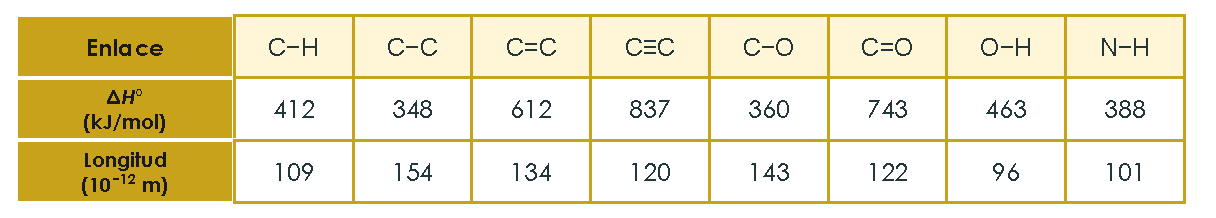
\includegraphics[width=0.95\linewidth]{FigurasSVG/UD3_Enlace_Quimico/pdf/UD3_13_entalpias_longitudes_enlace.pdf}
            \caption{Entalpías promedio y longitudes de enlace promedio.}
            \label{fig:entalpiasyenlaces}
        \end{figure}
        \item \negsubro{Polaridad de enlaces y moléculas}: se produce cuando existen electronegatividades diferentes entre dos átomos que forman un enlace introduciendo así una carga parcial positiva ($\delta +$)  en el elemento menos electronegativo o negativa ($\delta -$) en el elemento más electronegativo.

        Para cuantificar la polaridad de un enlace utilizaremos el \azuln{momento dipolar, $\mu$} que equivale al producto entre la carga neta ($q$) y la distancia internuclear ($r$) según la expresión.
        \begin{centeredequation}
            \tcboxmath[opteqA]{\mu = q\; r}
        \end{centeredequation}

        El momento dipolar es un vector orientado desde el polo positivo (átomo menos electronegativo) hacia el polo negativo (átomo más electronegativo).
        La unidad en el S.I es el \azuln{\si{\coulomb\metre}}.
        Hay que tener en cuenta que el momento dipolar nos da una medida de la polarización de dicho enlace y no hay que confundirlo con la \azuln{polaridad de una molécula}.
        Para saber si una molécula es polar, es decir presenta un momento dipolar distinto de cero, tenemos que sumar todos los momentos dipolares de todos los enlaces de la molécula y si el momento dipolar resultante es distinto de cero entonces diremos que la molécula es \azuln{polar} y si el resultado del momento dipolar resultante es cero, entonces decimos que la molécula es \azuln{apolar}
        \begin{figure}[H]
            \centering
            % [FIGURA ORIGINAL] \includegraphics[scale=1]{images/imagesUD3EnlaceQuimico/UD3_Teoria/polaridad_nuevo}
            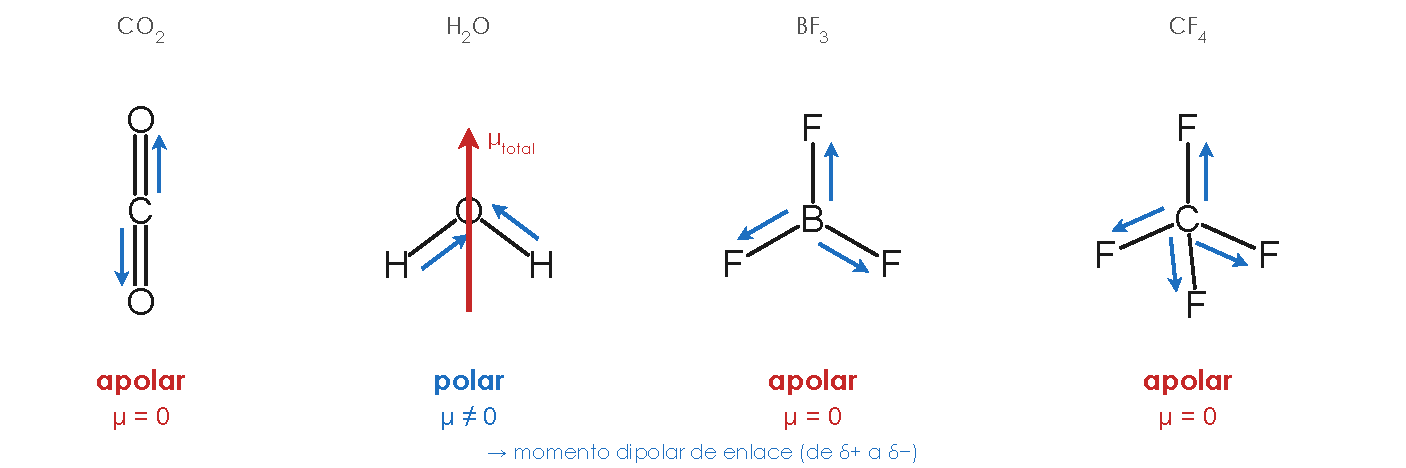
\includegraphics[width=0.9\linewidth]{FigurasSVG/UD3_Enlace_Quimico/pdf/UD3_14_polaridad_moleculas.pdf}
            \caption{Moléculas polares y apolares}
            \label{fig:moleculaspolaresyapolares}
        \end{figure}

        Los \textbf{pares de electrones no enlazantes} también contribuyen al momento dipolar de las moléculas, pues estos pares electrónicos tienden a concentrar la carga electrónica sobre el átomo al que pertenecen.
        Este efecto justifica por qué la molécula de \ch{NH3} tiene un momento dipolar mayor que \ch{NF3}

        Por norma general (aunque no siempre, habrá que estudiar cada caso en concreto), si sobre un átomo central los átomos a los que está unido no son todos iguales, la molécula suele ser \textbf{polar}, mientras que si son todos iguales, la polaridad dependerá de la geometría de la molécula y del número de pares de electrones enlazantes.
        En la siguiente tabla se muestra el tipo de polaridad que tendría una molécula si todos los átomos a los que se une el átomo central son iguales.

        % --- tabla antigua ---
        % \begin{longtblr}[
            % caption = {Polaridad de una molécula según su geometría cuando los átomos unidos al átomo central son iguales},
        % ]{
            % colspec = {|Q[c,m]|Q[c,m]|},
            % rowhead = 1,
            % row{1} = {bg=mybluecolour, fg = white, font=\sffamily},
        % %vlines = {1}{white},
        % }
            % \hline
            % Geometría                                   & Polaridad \\
            % \hline
            % Lineal                                      & Apolar    \\
            % \hline
            % Trigonal plana (triangular)                 & Apolar    \\
            % \hline
            % Angular                                     & Polar     \\
            % \hline
            % Tetraédrica                                 & Apolar    \\
            % \hline
            % Pirámide trigonal                           & Polar     \\
            % \hline
            % Bipirámide trigonal (bipirámide triangular) & Polar     \\
            % \hline
            % Tetraédrica distorsionada                   & Polar     \\
            % \hline
            % En forma de T                               & Polar     \\
            % \hline
            % Octaédrica                                  & Apolar    \\
            % \hline
            % Pirámide cuadrada                           & Polar     \\
            % \hline
            % Plano cuadrada                              & Apolar    \\
            % \hline
        % \end{longtblr}
        % --- tabla nueva ---
        \begin{longtable}{@{}cc@{}}
            \caption{Polaridad de una molécula según su geometría cuando los átomos unidos al átomo central son iguales} \\
            \toprule
            \textbf{Geometría} & \textbf{Polaridad} \\
            \midrule
            \endfirsthead
            \toprule
            \textbf{Geometría} & \textbf{Polaridad} \\
            \midrule
            \endhead
            \bottomrule
            \endlastfoot
            Lineal & Apolar \\[3pt]
            Trigonal plana (triangular) & Apolar \\[3pt]
            Angular & Polar \\[3pt]
            Tetraédrica & Apolar \\[3pt]
            Pirámide trigonal & Polar \\[3pt]
            Bipirámide trigonal (bipirámide triangular) & Polar \\[3pt]
            Tetraédrica distorsionada & Polar \\[3pt]
            En forma de T & Polar \\[3pt]
            Octaédrica & Apolar \\[3pt]
            Pirámide cuadrada & Polar \\[3pt]
            Plano cuadrada & Apolar \\
        \end{longtable}



        \item \negsubro{Polarizables y polarizantes}: podemos decir que un átomo o ion es \azuln{polarizable} cuando su nube electrónica experimenta fácilmente grandes deformaciones de modo que puede inducirse en un extremo del átomo más carga electrónica que en el otro extremo, dando lugar así a la aparición de un dipolo (molécula con un $\delta +$ y $\delta -$). En general, los iones grandes como el \ch{I-} son altamente polarizables.
        Un átomo o ion es \azuln{polarizante} cuando puede producir esas grandes deformaciones en las nubes electrónicas.
        Son buenos polarizantes los cationes pequeños y de carga elevada.
\end{enumerate}

%    \begin{enumerate}[label=\numberballmDarkBrown]
%        \item \negsubro{Radicales}: es un fragmento de molécula con algún electrón desapareado, provienen fundamentalmente de la ruptura homolítica de enlaces en el cual el par de electrones que formaban el enlace se reparte uno para cada átomo. Como ejemplos vemos el radical metilo y el radical hidroxilo.
%        \begin{figure}[H]
%            \centering
%            \includegraphics[scale=1]{images/imagesUD3EnlaceQuimico/UD3_Teoria/radicales.eps}
%            \caption{Radicales metilo e hidroxilo}
%            \label{fig:radicalmetilohidroxilo}
%        \end{figure}
%        \item \negrita{\coloruline{red}{Parámetros del enlace covalente}}
%        \begin{enumerate}
%            \item \negrita{Longitud de enlace}: distancia entre los átomos enlazados.
%            \item \negrita{Ángulo de enlace}: solo tiene sentido en moléculas de 3 o más átomos y será el ángulo que forman dos enlaces compartiendo un átomo común.
%            \item \negrita{Entalpía de enlace}: es la energía que se debe suministrar o se libera cuando se rompe un enlace, un enlace sencillo tendrá menos energía que un enlace doble y este a su vez que un enlace triple.
%            \begin{figure}[H]
%                \centering
%                \includegraphics[scale=0.45]{images/imagesUD3EnlaceQuimico/UD3_Teoria/entalpiasyenlacespromedio.png}
%                \caption{Entalpías promedio y longitudes de enlace promedio.}
%                \label{fig:entalpiasyenlaces}
%            \end{figure}
%        \end{enumerate}
%        \item \negsubro{Polaridad de enlaces y moléculas}: se produce cuando existen electronegatividades diferentes entre dos átomos que forman un enlace introduciendo así una carga parcial positiva ($\delta +$) o negativa ($\delta -$) en cada átomo.
%
%        Para cuantificar la polaridad de un enlace utilizaremos el \azuln{momento dipolar, $\mu$} que equivale al producto entre la carga neta ($q$) y la distancia internuclear ($r$) según la expresión.
%        \begin{equation}
%            \tcboxmath[opteqA]{\mu = q\; r}
%        \end{equation}
%        El momento dipolar es un vector orientado desde el polo positivo (átomo menos electronegativo) hacia el polo negativo (átomo más electronegativo). La unidad en el S.I es el \azuln{\si{\coulomb\metre}}.
%        Hay que tener en cuenta que el momento dipolar nos da una medida de la polarización de dicho enlace y no hay que confundirlo con la \azuln{polaridad de una molécula}. Para saber si una molécula es polar, es decir presenta un momento dipolar distinto de cero, tenemos que sumar todos los momentos dipolares de todos los enlaces de la molécula y si el momento dipolar resultante es distinto de cero entonces diremos que la molécula es \azuln{polar} y si el resultado del momento dipolar resultante es cero, entonces decimos que la molécula es \azuln{apolar}
%        \begin{figure}[H]
%            \centering
%            \includegraphics[scale=1]{images/imagesUD3EnlaceQuimico/UD3_Teoria/polaridad.eps}
%            \caption{Moléculas polares y apolares}
%            \label{fig:moleculaspolaresyapolares}
%        \end{figure}
%
%        Los \textbf{pares de electrones no enlazantes} también contribuyen al momento dipolar de las moléculas, pues estos pares electrónicos tienden a concentrar la carga electrónica sobre el átomo al que pertenecen. Este efecto justifica por qué la molécula de \ch{NH3} tiene un momento dipolar mayor que el \ch{NF3}
%
%        Por norma general (aunque no siempre, habrá que estudiar cada caso en concreto), si sobre un átomo central los átomos a los que está unido no son todos iguales, la molécula suele ser \textbf{polar}, mientras que si son todos iguales, la polaridad dependerá de la geometría de la molécula y del número de pares de electrones enlazantes. En la siguiente tabla se muestra el tipo de polaridad que tendría una molécula si todos los átomos a los que se une el átomo central son iguales.
%
%        \begin{longtblr}[
%            caption = {Polaridad de una molécula según su geometría cuando los átomos unidos al átomo central son iguales},
%        ]{
%            colspec = {|Q[c,m]|Q[c,m]|},
%            rowhead = 1,
%            row{1} = {bg=mybluecolour, fg = white, font=\sffamily},
%            vlines = {1}{white},
%        }
%            \hline
%            Geometría                                                                                                                                & Polaridad \\
%            \hline
%            {\includegraphics[scale=.5]{images/imagesUD3EnlaceQuimico/UD3_Teoria/lineal.png}  Lineal}                                                  & Apolar    \\
%            \hline
%            {\includegraphics[scale=0.5]{images/imagesUD3EnlaceQuimico/UD3_Teoria/trigonal.png}  Trigonal plana (triangular)}                          & Apolar     \\
%            \hline
%            {\includegraphics[scale=0.5]{images/imagesUD3EnlaceQuimico/UD3_Teoria/angular.png} Angular}                                                & Polar     \\
%            \hline
%            {\includegraphics[scale=0.5]{images/imagesUD3EnlaceQuimico/UD3_Teoria/tetraedrica.png} Tetraédrica }                                       & Apolar    \\
%            \hline
%            {\includegraphics[scale=.5]{images/imagesUD3EnlaceQuimico/UD3_Teoria/piramidetrigonal.png}  Pirámide trigonal}                             & Polar     \\
%            \hline
%            {\includegraphics[scale=.5]{images/imagesUD3EnlaceQuimico/UD3_Teoria/bipiramidetrigonal.png}  Bipirámide trigonal (bipirámide triangular)} & Polar     \\
%            \hline
%            {\includegraphics[scale=.5]{images/imagesUD3EnlaceQuimico/UD3_Teoria/tetraedricadistorsionada.png} Tetraédrica distorsionada }             & Polar     \\
%            \hline
%            {\includegraphics[scale=.5]{images/imagesUD3EnlaceQuimico/UD3_Teoria/enformadeT} En forma de T}                                        & Polar     \\
%            \hline
%            {\includegraphics[scale=.5]{images/imagesUD3EnlaceQuimico/UD3_Teoria/octaedrica.png}  Octaédrica}                                          & Apolar    \\
%            \hline
%            {\includegraphics[scale=.5]{images/imagesUD3EnlaceQuimico/UD3_Teoria/piramidalcuadrada.png}  Pirámide cuadrada}                            & Polar     \\
%            \hline
%            {\includegraphics[scale=.5]{images/imagesUD3EnlaceQuimico/UD3_Teoria/planacuadrada.png}  Plano cuadrada}                                   & Apolar    \\
%            \hline
%        \end{longtblr}
%
%
%
%        \item \negsubro{Polarizables y polarizantes}: podemos decir que un átomo o ion es \azuln{polarizable} cuando su nube electrónica experimenta fácilmente grandes deformaciones de modo que puede inducirse en un extremo del átomo más carga electrónica que en el otro extremo y por lo tanto aparición de un dipolo (molécula con un $\delta +$ y $\delta -$). En general, los iones grandes como el \ch{I-} son altamente polarizables.
%        Un átomo o ion es \azuln{polarizante} cuando puede producir esas grandes deformaciones en las nubes electrónicas.
%        Son buenos polarizantes los cationes pequeños y elevadas cargas.
%    \end{enumerate}

\subsection{Enlace covalente dativo o coordinado}

En un \azuln{enlace covalente dativo} es aquel en el que los dos electrones son donados por un átomo. Para que el enlace se produzca uno de los átomos tiene que disponer de un par electrones libre y el otro debe disponer de un orbital libre para aceptarlos.

El enlace covalente dativo se representa mediante una flecha que va desde el átomo donador al átomo aceptor ($A \rightarrow B$)

%    \begin{figure}[H]
%        \centering
%        \includegraphics[scale=1]{images/imagesUD3EnlaceQuimico/UD3_Teoria/dativoamonio}
%        \caption{Enlace covalente dativo}
%        \label{fig:enlacecovalentedativo}
%    \end{figure}


% \begin{figure}[H]
%     \centering
%     \includegraphics[scale=1]{covalente dativo.png}
%     \caption{Enlace covalente dativo}
%     \label{fig:enlacecovalentedativo}
% \end{figure}

Ejemplos de la formación del enlace covalente dativo, lo podemos encontrar en:
\begin{enumerate}[label=\numberballmDarkBrown]
        \item \negsubro{Ion Amonio (\ch{NH4^+})}:
        \begin{figure}[H]
            \centering
            % [FIGURA ORIGINAL] \includegraphics[scale=.5]{images/imagesUD3EnlaceQuimico/UD3_Teoria/dativoamonio}
            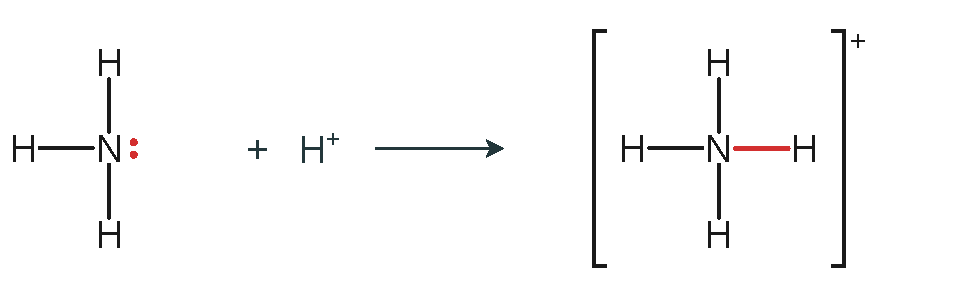
\includegraphics[width=0.7\linewidth]{FigurasSVG/UD3_Enlace_Quimico/pdf/UD3_15_dativo_amonio.pdf}
            \caption{Enlace dativo en el ion amonio}
            \label{fig:dativoamonio}
        \end{figure}
        \item \negsubro{Ion Oxonio (\ch{H3O^+})}:
        \begin{figure}[H]
            \centering
            % [FIGURA ORIGINAL] \includegraphics[scale=.5]{images/imagesUD3EnlaceQuimico/UD3_Teoria/dativooxonio}
            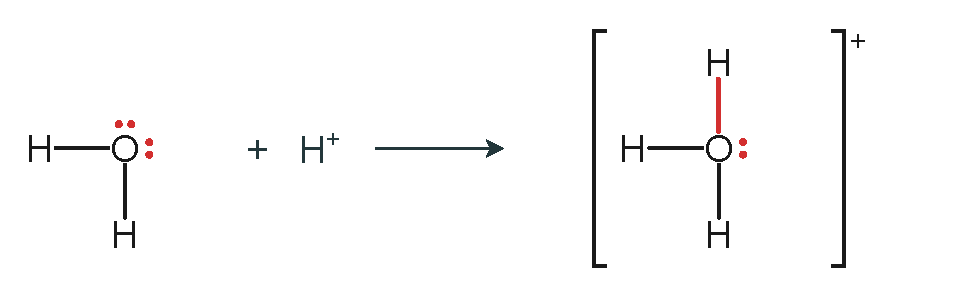
\includegraphics[width=0.7\linewidth]{FigurasSVG/UD3_Enlace_Quimico/pdf/UD3_16_dativo_oxonio.pdf}
            \caption{Enlace dativo en el ion oxonio}
            \label{fig:dativoxonio}
        \end{figure}
\end{enumerate}

\subsection{Teoría de la repulsión entre pares de electrones de valencia (TRPECV)}\label{subsec:teoria-de-la-repulsion-entre-pares-de-electrones-de-valencia-(trpecv)}

Todos los pares electrónicos (enlazantes y no enlazantes) de la capa de valencia de los átomos que forman los enlaces covalentes se sitúan lo más alejado posible unos de los otros, de manera que las repulsiones sean las mínimas. Esta teoría explica la \rojon{geometría} de las sustancias covalentes

El factor determinante de la geometría de la molécula es el número de pares de electrones de valencia, tanto enlazantes como no enlazantes que tenemos alrededor del átomo central.
En la siguiente figura, podemos ver como las repulsiones electrónicas entre los pares de electrones no enlazantes y los enlazantes-no enlazantes en la molécula de agua hacen que el ángulo teórico de \ang{180} se cierre quedando finalmente en un ángulo real de \ang{104.5}.
Esta geometría es angular y no lineal.
\begin{figure}[H]
    \centering
    % [FIGURA ORIGINAL] \includegraphics[scale=0.5]{images/imagesUD3EnlaceQuimico/UD3_Teoria/respulsiones electrónicas}
    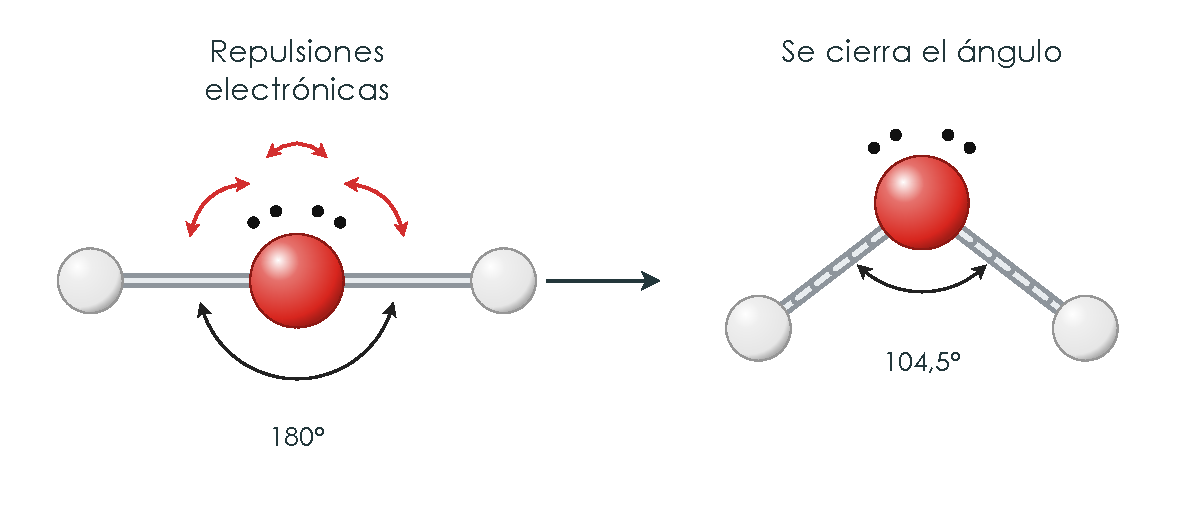
\includegraphics[width=0.75\linewidth]{FigurasSVG/UD3_Enlace_Quimico/pdf/UD3_17_repulsiones_electronicas.pdf}
    \caption{Repulsiones electrónicas en la molécula de agua.}
    \label{fig:repulsionesagua}
\end{figure}

%    {\large{} \textbf{\textcolor{blue}{Postulados del modelo TRPECV}}}

% Los postulados básicos de la TRPECV son:
%    \begin{enumerate}[label=\numberballmDarkBrown]
%        \item El factor determinante de la geometría de la molécula es el número de pares de electrones de valencia, tanto enlazantes como no enlazantes que tenemos alrededor del átomo central.
%        \item Se cuenta el número de zonas de alta densidad electrónica entorno al átomo central sin distinguir entre enlaces y pares de electrones solitarios.
%        \item Se representan gráficamente las orientaciones espaciales de mínima repulsión (los pares no compartidos ocupan más espacio que los compartidos).
%        \item Se colocan los átomos que rodean al átomo central en los extremos de las nubes electrónicas.
%        \item Se obtiene la geometría molecular a partir de la disposición espacial de los núcleos de los átomos presentes (no de las nubes electrónicas). La geometría real se predice teniendo en cuenta las distorsiones angulares generadas por los diferentes pares de enlace o pares solitarios.
%
%        En la siguiente figura, podemos ver como las repulsiones electrónicas entre los pares de electrones no enlazantes y los enlazantes-no enlazantes en la molécula de agua hacen que el ángulo teórico de \ang{180} se cierre quedando finalmente en un ángulo real de \ang{104.5}. Esta geometría es angular y no lineal.
%        \begin{figure}[H]
%            \centering
%            \includegraphics[scale=0.5]{images/imagesUD3EnlaceQuimico/UD3_Teoria/respulsiones electrónicas.png}
%            \caption{Repulsiones electrónicas en la molécula de agua.}
%            \label{fig:repulsionesagua}
%        \end{figure}
%    \end{enumerate}

\subsubsection[Geometría sin pares de electrones no enlazantes]{Geometría de las moléculas cuyo átomo central carece de pares de electrones solitarios o no enlazantes}

Vamos a suponer que la molécula a estudiar tiene un átomo central (A) y unido a el, otro átomo o conjunto de átomos (pueden ser iguales o diferentes) que los nombraremos como B.
Al no tener pares de electrones no enlazantes la geometría general de la molécula la podemos escribir como \ch{AB_n} donde $n$ puede variar entre 2 y 6.
Siendo \( n \) el número de átomo unidos al átomo central que pueden ser todos iguales o diferentes, por ejemplo la molécula \ch{H2O} sería del tipo \( AB_2 \) (el \ch{O} es el átomo central \( A \) mientras que los hidrógenos serán los átomos \( B \) ), la molécula \ch{CH4} (el \ch{C} es el átomo central \( A \) y los hidrógenos los átomos \( B \)) sería del tipo \( AB_4 \) y la molécula \ch{BF2Cl} (el átomo central \( A  \) sería el boro mientras que que los átomos \( B \) serían en este caso el \ch{F} y el \ch{Cl}) sería del tipo \( AB_3 \)

\begin{enumerate}[label=\numberballmDarkTeal]
        \item \negrita{Molécula del tipo \ch{AB2}}: son moléculas con geometría \azuln{lineal} y tienen un ángulo de \rojon{\ang{180}}.
        Ejemplos: \ch{CO2}, \ch{BeH2}.
        \begin{figure}[H]
            \centering
            % [FIGURA ORIGINAL] \includegraphics[scale=0.5]{images/imagesUD3EnlaceQuimico/UD3_Teoria/GEOMETriaCO2}
            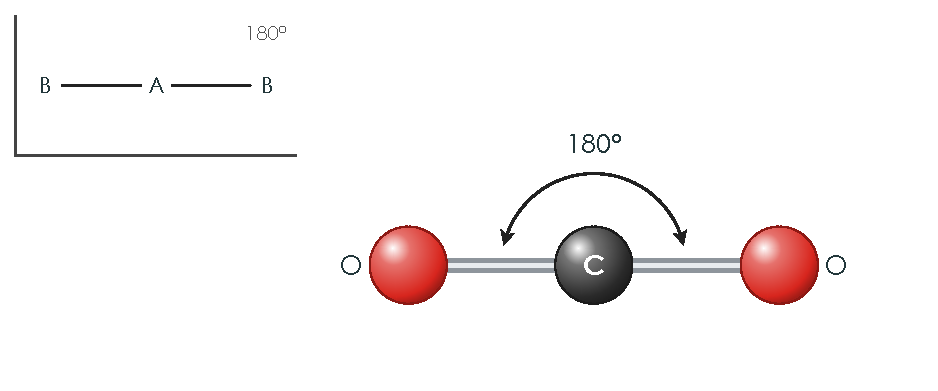
\includegraphics[width=0.6\linewidth]{FigurasSVG/UD3_Enlace_Quimico/pdf/UD3_18_geometria_CO2.pdf}
            \caption{Geometría de la molécula \ch{CO2}}
            \label{fig:GeometriadelamoleculaCO2}
        \end{figure}
        \item \negrita{Molécula del tipo \ch{AB3}}: son moléculas con geometría \azuln{trigonal plana}, con ángulos de enlace de \rojon{\ang{120}}. Ejemplos: \ch{BCl3}, \ch{NO3-}, \ch{CO3^{2-}}, \ch{BI3}, \ch{BH3}.
        \begin{figure}[H]
            \centering
            % [FIGURA ORIGINAL] \includegraphics[scale=0.5]{images/imagesUD3EnlaceQuimico/UD3_Teoria/trigonal_BI3}
            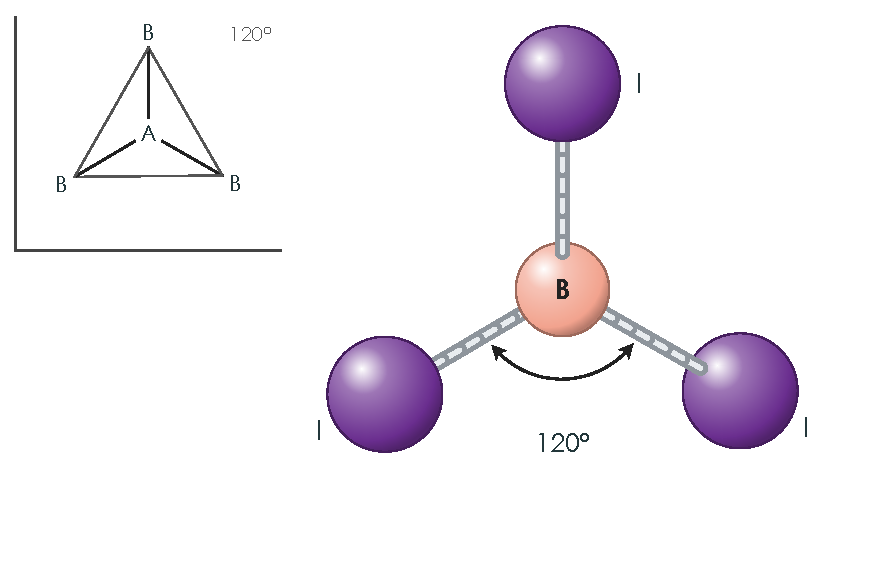
\includegraphics[width=0.6\linewidth]{FigurasSVG/UD3_Enlace_Quimico/pdf/UD3_19_geometria_trigonal_BI3.pdf}
            \caption{Geometría de la molécula \ch{BI3}}
            \label{fig:trigonalBI3}
        \end{figure}
        \item \negrita{Molécula del tipo \ch{AB4}}: son moléculas con geometría \azuln{tetraédrica} con ángulos de enlace de \rojo{\ang{109.5}}.
        Ejemplos: \ch{CH4}, \ch{NH4^+}, \ch{CCl4}, \ch{SO4^{2-}}.
        \begin{figure}[H]
            \centering
            % [FIGURA ORIGINAL] \includegraphics[scale=0.5]{images/imagesUD3EnlaceQuimico/UD3_Teoria/tetraedrica_CCl4}
            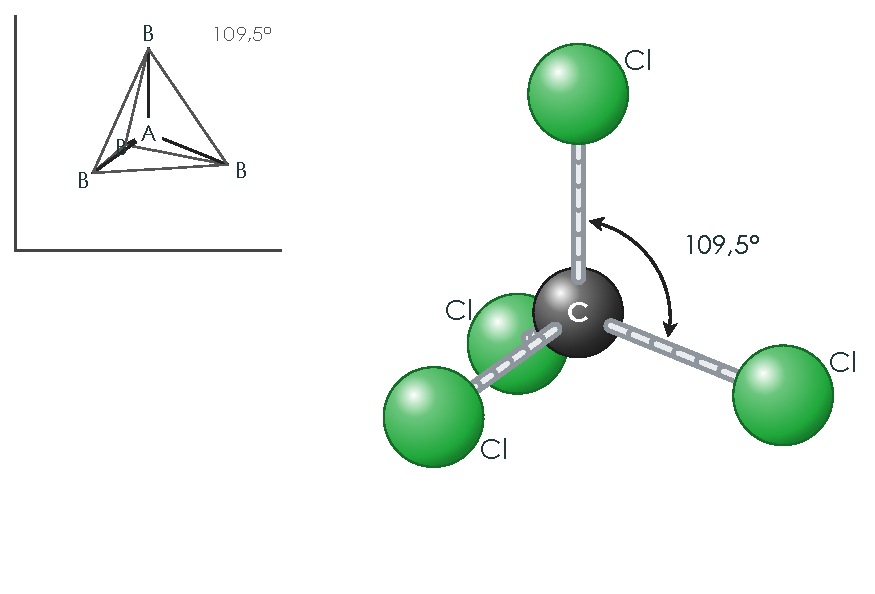
\includegraphics[width=0.6\linewidth]{FigurasSVG/UD3_Enlace_Quimico/pdf/UD3_20_geometria_tetraedrica_CCl4.pdf}
            \caption{Geometría de la molécula \ch{CCl4}}
            \label{fig:geometriaccl4}
        \end{figure}
        \item \negrita{Molécula del tipo \ch{AB5}}: tienen geometría \azuln{bipirámide trigonal}.
        Coexisten dos ángulos tipos de ángulos, unos de \rojo{\ang{120}} y otros de \rojo{\ang{90}}.
        Ejemplo: \ch{PCl5}
        \begin{figure}[H]
            \centering
            % [FIGURA ORIGINAL] \includegraphics[scale=0.5]{images/imagesUD3EnlaceQuimico/UD3_Teoria/bipiramidetrigonal_PCl5}
            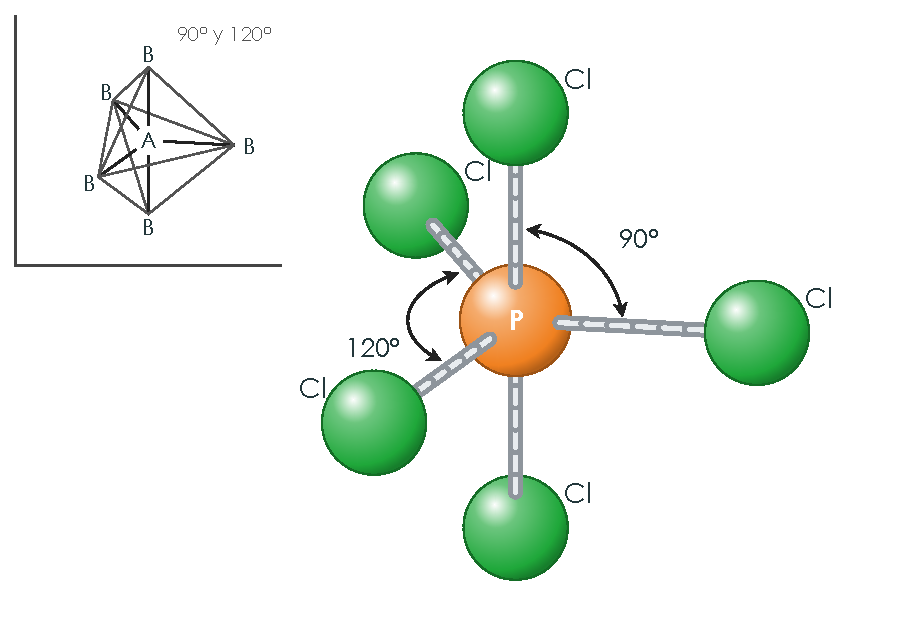
\includegraphics[width=0.6\linewidth]{FigurasSVG/UD3_Enlace_Quimico/pdf/UD3_21_geometria_bipiramide_PCl5.pdf}
            \caption{Geometría de la molécula \ch{PCl5}}
            \label{fig:GeometriadelPCl5}
        \end{figure}
        \item \negrita{Molécula del tipo \ch{AB6}}: son moléculas con geometría \azuln{octaédrica} con ángulos de enlace de \rojo{\ang{90}}.
        Ejemplos: \ch{SF6}
        \begin{figure}[H]
            \centering
            % [FIGURA ORIGINAL] \includegraphics[scale=0.5]{images/imagesUD3EnlaceQuimico/UD3_Teoria/octaedrica_SF6}
            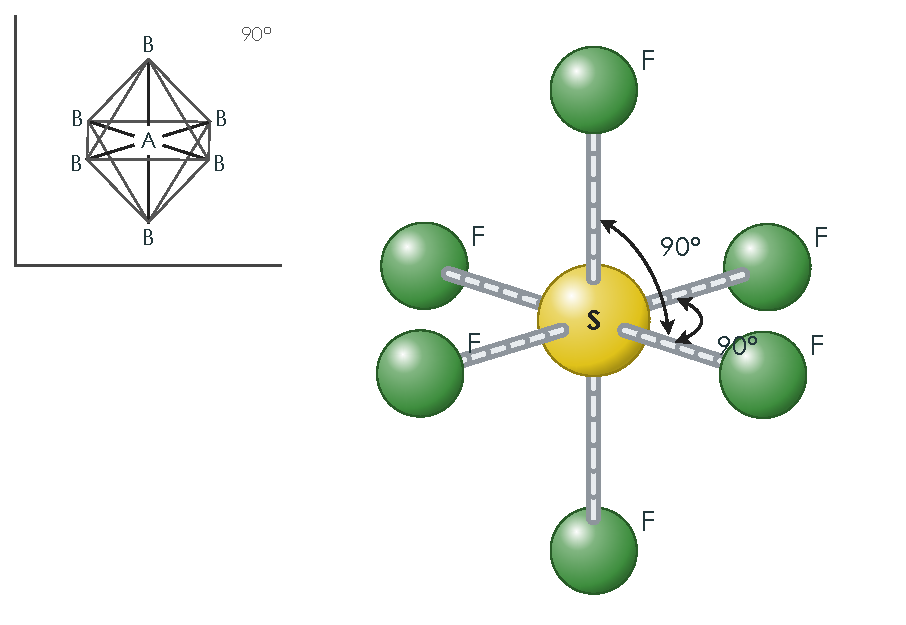
\includegraphics[width=0.6\linewidth]{FigurasSVG/UD3_Enlace_Quimico/pdf/UD3_22_geometria_octaedrica_SF6.pdf}
            \caption{Geometría de la molécula \ch{SF6}}
            \label{fig:GeometriadelamoleculaSF6}
        \end{figure}
\end{enumerate}

\subsubsection[Geometría con pares de electrones no enlazantes]{Geometría de moléculas cuyo átomo central tiene pares de electrones no compartidos o solitarios}
La presencia de pares no enlazantes en una molécula varía el ángulo de enlace por efecto de la repulsión electrónica y por lo tanto modifica su geometría molecular.
Los ángulos disminuyen a medida de que aumenta el número de pares de electrones no enlazantes o no compartidos.

Si usamos el símbolo X para describir los pares de electrones no enlazantes del átomo central, la fórmula general de estas moléculas será: \ch{AB_nX_m}.

\begin{enumerate}[label=\numberballmDarkTeal]
        \item \negrita{Molécula del tipo \ch{AB2X}}: son moléculas con geometría \azuln{angular} y tienen un ángulo de enlace \verden{menor} de \rojon{\ang{120}}.
        Ejemplos: \ch{SO2}, \ch{O3}, \ch{NO2-}, \ch{SnCl2}, \ch{IBr2-}, \ch{ClO2-}.
        \begin{figure}[H]
            \centering
            % [FIGURA ORIGINAL] \includegraphics[scale=0.5]{images/imagesUD3EnlaceQuimico/UD3_Teoria/angular_O3}
            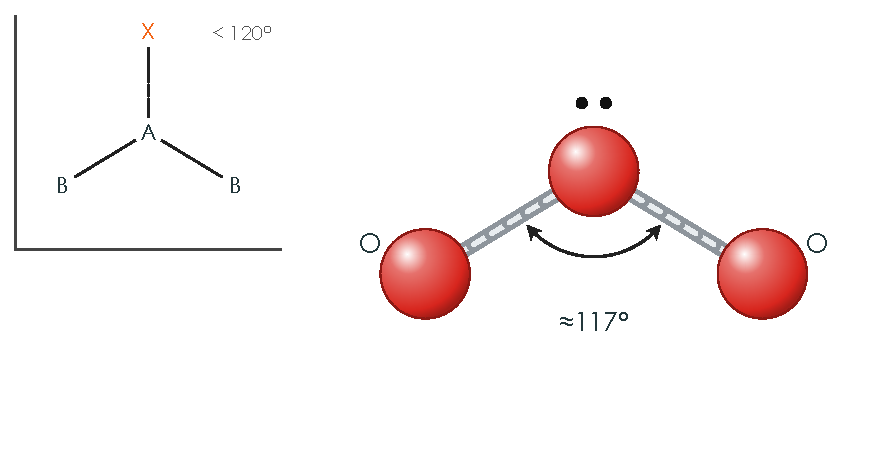
\includegraphics[width=0.6\linewidth]{FigurasSVG/UD3_Enlace_Quimico/pdf/UD3_23_geometria_angular_O3.pdf}
            \caption{Geometría de la molécula \ch{O3}}
            \label{fig:GeometriadelamoleculaO3}
        \end{figure}
        \item \negrita{Molécula del tipo \ch{AB3X}}: son moléculas con una geometría de \azuln{pirámide trigonal}, con ángulos de enlace \verden{menores} de  \rojon{\ang{109.5}}.
        Ejemplos: \ch{NH3}, \ch{H3O+}, \ch{AsH3}, \ch{PH3}, \ch{NF3}, \ch{PBr3}, \ch{PF3}, \ch{ClO3-}.
        \begin{figure}[H]
            \centering
            % [FIGURA ORIGINAL] \includegraphics[scale=0.5]{images/imagesUD3EnlaceQuimico/UD3_Teoria/priamidetrigonal_NH3}
            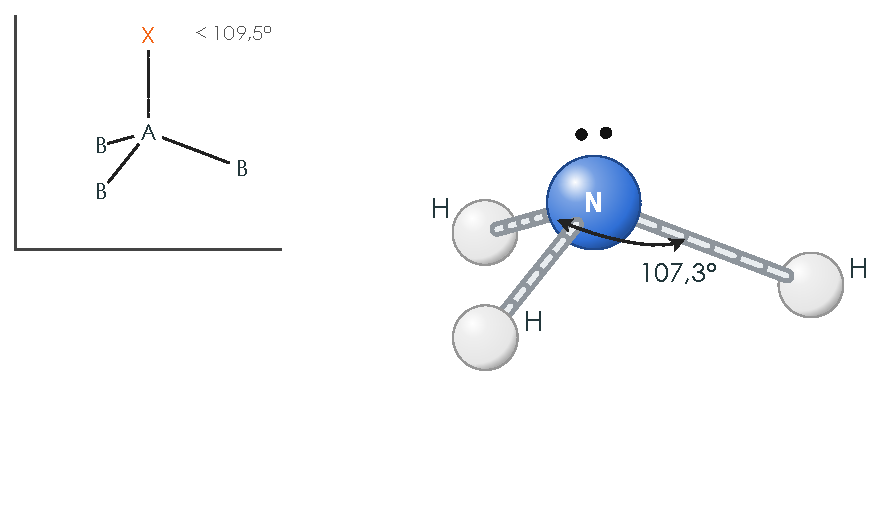
\includegraphics[width=0.6\linewidth]{FigurasSVG/UD3_Enlace_Quimico/pdf/UD3_24_geometria_piramide_NH3.pdf}
            \caption{Geometría de la molécula \ch{NH3}}
            \label{fig:geometriaNH3}
        \end{figure}
        \item \negrita{Molécula del tipo \ch{AB2X2}}: son moléculas con geometría \azuln{angular} con ángulos de enlace \verden{menor} de \rojo{\ang{120}}.
        Ejemplos: \ch{H2O}, \ch{H2S}, \ch{SF2}.
        \begin{figure}[H]
            \centering
            % [FIGURA ORIGINAL] \includegraphics[scale=0.5]{images/imagesUD3EnlaceQuimico/UD3_Teoria/angular_H2S}
            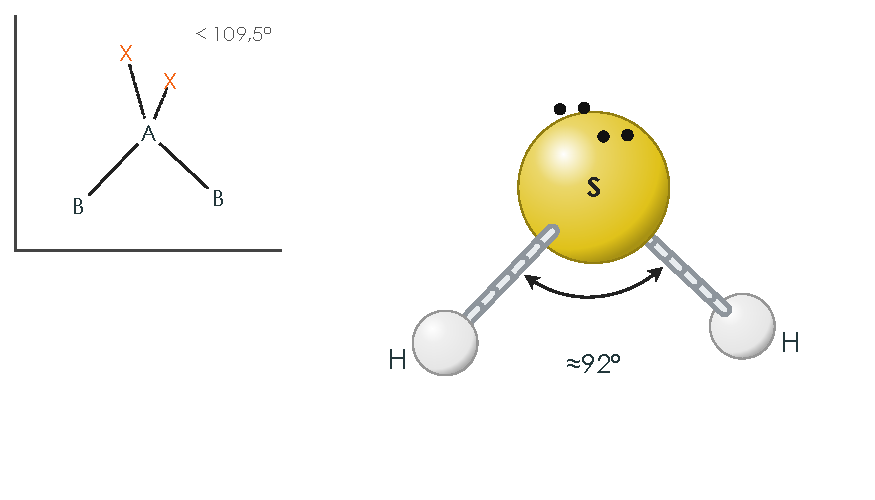
\includegraphics[width=0.6\linewidth]{FigurasSVG/UD3_Enlace_Quimico/pdf/UD3_25_geometria_angular_H2S.pdf}
            \caption{Geometría de la molécula \ch{H2S}}
            \label{fig:geometriaH2S}
        \end{figure}
\end{enumerate}


A modo de resumen en la siguiente tabla se incluyen todos los casos.

%    \begin{longtblr}[
%        caption = {Tabla resumen de la geometría según la TRPECV},
%    ]
%    {
%        colspec = {|Q[c,m]|Q[c,m]|Q[c,m]|Q[c,m]|Q[c,m]|},
%        rowhead = 1,
%        row{1} = {bg=mybluecolour, fg = white, font=\sffamily},
%        vlines = {1}{white},
%    }
%        \hline
%        {\textbf{nº total de} \\ \textbf{pares de \el}}                  & {\textbf{nº total de pares} \\ \textbf{de \el enlazantes}} & {\textbf{nº total de pares} \\ \textbf{de \el no enlazantes}}                   & \textbf{Geometría} & \textbf{Ejemplo} \\
%        \hline
%        2 & 2 & 0 & {\includegraphics[scale=.5]{images/imagesUD3EnlaceQuimico/UD3_Teoria/lineal.png}                                                      Lineal}                       & \ch{BeF2}  \\
%        \hline
%        \SetCell[r=2]{m} 3                   & 3 & 0 & {\includegraphics[scale=.5]{images/imagesUD3EnlaceQuimico/UD3_Teoria/trigonal.png}                                                     Trigonal plana (triangular)} & \ch{BF3}  \\
%        \hline
%        & 2 & 1 & {\includegraphics[scale=.5]{images/imagesUD3EnlaceQuimico/UD3_Teoria/angular.png} Angular   }                                  & \ch{SnCl2}   \\
%        \hline
%        \SetCell[r=3]{m} 4 & 4 & 0 & {\includegraphics[scale=.5]{images/imagesUD3EnlaceQuimico/UD3_Teoria/tetraedrica.png} Tetraédrica }                                                                 & \ch{CH4}   \\
%        \hline
%        & 3 & 1 & {\includegraphics[scale=.5]{images/imagesUD3EnlaceQuimico/UD3_Teoria/piramidetrigonal.png} Pirámide trigonal }                                                      & \ch{NH3}   \\
%        \hline
%        & 2 & 2 & {\includegraphics[scale=.5]{images/imagesUD3EnlaceQuimico/UD3_Teoria/angularb.png} Angular }                           & \ch{H2O}  \\
%        \hline
%        \SetCell[r=4]{m} 5                   & 5 & 0 & {\includegraphics[scale=.5]{images/imagesUD3EnlaceQuimico/UD3_Teoria/bipiramidetrigonal.png} Bipirámide triangular}                                     & \ch{PCl5}  \\
%        \hline
%        & 4 & 1 & {\includegraphics[scale=.5]{images/imagesUD3EnlaceQuimico/UD3_Teoria/tetraedricadistorsionada.png} Tetraédrica distorsionada}                                       & \ch{SF4}   \\
%        \hline
%        & 3 & 2 & {\includegraphics[scale=.5]{images/imagesUD3EnlaceQuimico/UD3_Teoria/enformadeT.png} En forma de T  }                                                               & \ch{ClF3}  \\
%        \hline
%        & 2 & 3 & {\includegraphics[scale=.5]{images/imagesUD3EnlaceQuimico/UD3_Teoria/linealb.png} Lineal  }                       & \ch{XeF2}  \\
%        \hline
%        \SetCell[r=3]{m}6                   & 6 & 0 & {\includegraphics[scale=.5]{images/imagesUD3EnlaceQuimico/UD3_Teoria/octaedrica.png} Octaédrica}                       & \ch{SF6}  \\
%        \hline
%        & 5 & 1 & {\includegraphics[scale=.5]{images/imagesUD3EnlaceQuimico/UD3_Teoria/piramidalcuadrada.png} Pirámide cuadrada}                       & \ch{ICl5}  \\
%        \hline
%        & 4 & 2 & {\includegraphics[scale=.5]{images/imagesUD3EnlaceQuimico/UD3_Teoria/planacuadrada.png} Plano cuadrada}                       & \ch{XeF4}  \\
%        \hline
%    \end{longtblr}

% --- tabla antigua ---
% \begin{longtblr}[
    % caption = {Tabla resumen de la geometría según la TRPECV},
% ]
% {
    % colspec = {|Q[c,m]|Q[c,m]|Q[c,m]|Q[c,m]|Q[c,m]|},
    % rowhead = 1,
    % row{1} = {bg=mybluecolour, fg = white},
    % vlines = {1}{white},
% }
    % \hline
    % {\textbf{nº total de} \\ \textbf{pares de \el}}                  & {\textbf{nº total de pares} \\ \textbf{de \el enlazantes}} & {\textbf{nº total de pares} \\ \textbf{de \el no enlazantes}}                   & \textbf{Geometría} & \textbf{Ejemplo} \\
    % \hline
    % 2 & 2 & 0 & Lineal                 & \ch{BeF2}   \\
    % \hline
    % \SetCell[r=2]{m} 3                   & 3 & 0 & Trigonal plana (triangular)           & \ch{BF3}   \\
    % \hline
    % & 2 & 1 & Angular                     & \ch{SnCl2}   \\
    % \hline
    % \SetCell[r=3]{m} 4 & 4 & 0 & Tetraédrica       & \ch{CH4}  \\
    % \hline
    % & 3 & 1 & Pirámide trigonal   & \ch{NH3}   \\
    % \hline
    % & 2 & 2 & Angular               & \ch{H2O}  \\
    % \hline
    % \SetCell[r=4]{m} 5                   & 5 & 0 & Bipirámide triangular                      & \ch{PCl5}  \\
    % \hline
    % & 4 & 1 & Tetraédrica distorsionada                  & \ch{SF4}   \\
    % \hline
    % & 3 & 2 & En forma de T           & \ch{ClF3}  \\
    % \hline
    % & 2 & 3 & Lineal              & \ch{XeF2}  \\
    % \hline
    % \SetCell[r=3]{m}6                   & 6 & 0 & Octaédrica              & \ch{SF6}  \\
    % \hline
    % & 5 & 1 & Pirámide cuadrada              & \ch{ICl5}  \\
    % \hline
    % & 4 & 2 & Plano cuadrada              & \ch{XeF4}  \\
    % \hline
% \end{longtblr}
% --- tabla nueva ---
\begin{longtable}{@{}ccccc@{}}
    \caption{Tabla resumen de la geometría según la TRPECV} \\
    \toprule
    \makecell{\textbf{nº total de} \\ \textbf{pares de \el}} & \makecell{\textbf{nº total de pares} \\ \textbf{de \el enlazantes}} & \makecell{\textbf{nº total de pares} \\ \textbf{de \el no enlazantes}} & \textbf{Geometría} & \textbf{Ejemplo} \\
    \midrule
    \endfirsthead
    \toprule
    \makecell{\textbf{nº total de} \\ \textbf{pares de \el}} & \makecell{\textbf{nº total de pares} \\ \textbf{de \el enlazantes}} & \makecell{\textbf{nº total de pares} \\ \textbf{de \el no enlazantes}} & \textbf{Geometría} & \textbf{Ejemplo} \\
    \midrule
    \endhead
    \bottomrule
    \endlastfoot
    2 & 2 & 0 & Lineal & \ch{BeF2} \\[3pt]
    \multirow{2}{*}{3} & 3 & 0 & Trigonal plana (triangular) & \ch{BF3} \\[3pt]
     & 2 & 1 & Angular & \ch{SnCl2} \\[3pt]
    \multirow{3}{*}{4} & 4 & 0 & Tetraédrica & \ch{CH4} \\[3pt]
     & 3 & 1 & Pirámide trigonal & \ch{NH3} \\[3pt]
     & 2 & 2 & Angular & \ch{H2O} \\[3pt]
    \multirow{4}{*}{5} & 5 & 0 & Bipirámide triangular & \ch{PCl5} \\[3pt]
     & 4 & 1 & Tetraédrica distorsionada & \ch{SF4} \\[3pt]
     & 3 & 2 & En forma de T & \ch{ClF3} \\[3pt]
     & 2 & 3 & Lineal & \ch{XeF2} \\[3pt]
    \multirow{3}{*}{6} & 6 & 0 & Octaédrica & \ch{SF6} \\[3pt]
     & 5 & 1 & Pirámide cuadrada & \ch{ICl5} \\[3pt]
     & 4 & 2 & Plano cuadrada & \ch{XeF4} \\
\end{longtable}


\begin{example}
    \textbf{Indica la geometría molecular de los compuestos \ch{SF2}, \ch{SF4}, \ch{SF6} según la TRPECV.}
    \vspace*{6pt}

    En general para resolver este tipo de ejercicios, deberemos seguir los siguientes pasos:

    \begin{enumerate}
        \item Realizar la estructura de lewis de la molécula.
        \item Contabilizar el número de pares de electrones enlazantes, no enlazantes y pares de electrones totales alrededor del átomo central.
        \item Asignar la geometría según la tabla dada anteriormente.
    \end{enumerate}

    \begin{itemize}
        \item \ch{SF2}.
        \begin{itemize}
            \item Estructura de Lewis:

            % [FIGURA ORIGINAL] \includegraphics[scale=1]{images/imagesUD3EnlaceQuimico/UD3_Teoria/ejemplo3_1}
            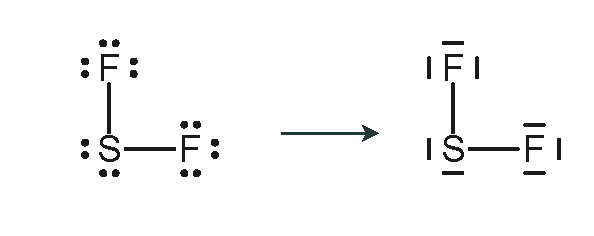
\includegraphics[width=0.4\linewidth]{FigurasSVG/UD3_Enlace_Quimico/pdf/UD3_26_ejemplo_SF2.pdf}

            \item Contabilización del número de pares de electrones.
            \begin{itemize}
                \item Pares de electrones totales = 4
                \item Pares de electrones no enlazantes = 2
                \item Pares de electrones enlazantes = 2
            \end{itemize}
            \item La geometría será en este caso \textbf{angular}.
        \end{itemize}

        \item \ch{SF4}

        \begin{itemize}
            \item Estructura de Lewis:

            % [FIGURA ORIGINAL] \includegraphics[scale=1]{images/imagesUD3EnlaceQuimico/UD3_Teoria/ejemplo3_1_b}
            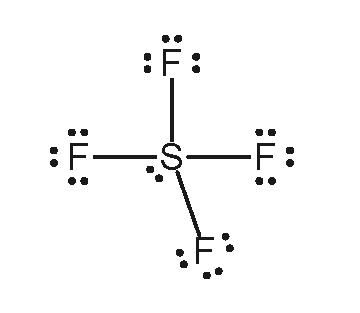
\includegraphics[width=0.25\linewidth]{FigurasSVG/UD3_Enlace_Quimico/pdf/UD3_27_ejemplo_SF4.pdf}

            \item Contabilización del número de pares de electrones.
            \begin{itemize}
                \item Pares de electrones totales = 5
                \item Pares de electrones no enlazantes = 1
                \item Pares de electrones enlazantes = 4
            \end{itemize}
            \item La geometría será en este caso \textbf{tetraédrica distorsionada}.
        \end{itemize}

        \item \ch{SF6}

        \begin{itemize}
            \item Estructura de Lewis:

            % [FIGURA ORIGINAL] \includegraphics[scale=1]{images/imagesUD3EnlaceQuimico/UD3_Teoria/ejemplo3_1_c}
            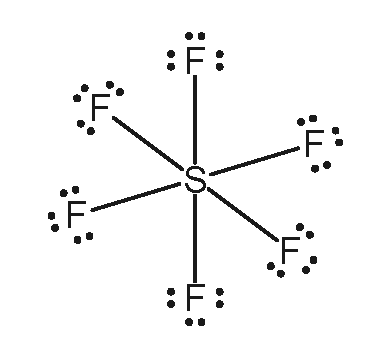
\includegraphics[width=0.27\linewidth]{FigurasSVG/UD3_Enlace_Quimico/pdf/UD3_28_ejemplo_SF6.pdf}

            \item Contabilización del número de pares de electrones.
            \begin{itemize}
                \item Pares de electrones totales = 6
                \item Pares de electrones no enlazantes = 0
                \item Pares de electrones enlazantes = 6
            \end{itemize}
            \item La geometría será en este caso \textbf{octaédrica}.
        \end{itemize}

    \end{itemize}

\end{example}

\subsection{Teoría del enlace de valencia (TEV)}\label{subsec:teoria-del-enlace-de-valencia-(tev)}

En la sección anterior, hemos visto como la TRPECV nos permitía explicar la geometría de la molécula analizando la disposición de los pares de electrones del átomo central, pero ¿en qué orbitales se sitúan esos electrones?

Para resolver este y otros problemas \textbf{Linus Pauling} propuso la teoría del enlace de valencia.

\begin{center}
    \begin{definition}[Enlace covalente]
        Un enlace covalente es el solapamiento de un orbital de un átomo con otro orbital de otro átomo, de modo que en los dos orbitales solapados existan dos electrones con sus momentos de \textit{spin} apareados
    \end{definition}
\end{center}


\begin{figure}[H]
    \centering
    % [FIGURA ORIGINAL] \includegraphics[scale=1]{images/imagesUD3EnlaceQuimico/UD3_Teoria/F2TEV}
    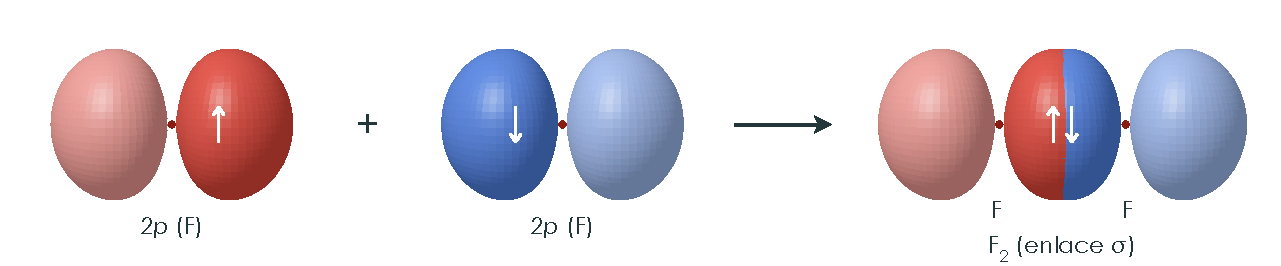
\includegraphics[width=0.8\linewidth]{FigurasSVG/UD3_Enlace_Quimico/pdf/UD3_29_F2_TEV_orbitales.pdf}
    \caption{Los orbitales se aproximan en la orientación adecuada. Se forma un enlace entre los dos átomos de flúor.}\label{fig:f2tev}
\end{figure}

Según el tipo de solapamiento, podemos encontrar dos tipos de enlace:
\begin{enumerate}
    \item \negsubro{Enlace tipo sigma ($\sigma$)}.
    Si ambos orbitales se solapan frontalmente, es decir, en el eje internuclear.
    Ejemplos: orbital $s$ con orbital $s$ (\chemfig{H-H}), orbital $s$ con orbital $p$ (\chemfig{H-Cl}) o orbital $p$ con orbital $p$ (\chemfig{Cl-Cl}).
    \begin{figure}[H]
        \centering
        % [FIGURA ORIGINAL] \includegraphics[scale=0.5]{images/imagesUD3EnlaceQuimico/UD3_Teoria/enlacesigma}
        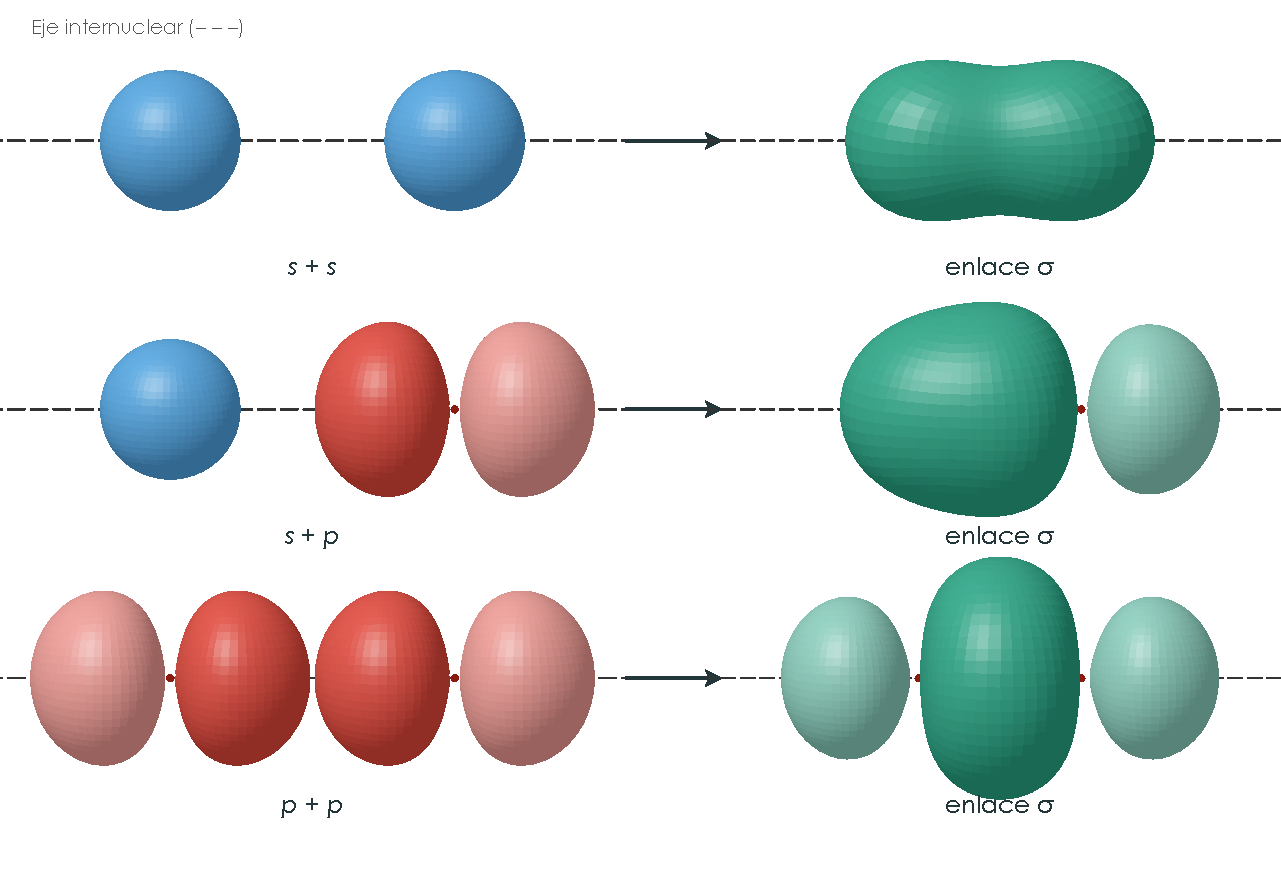
\includegraphics[width=0.8\linewidth]{FigurasSVG/UD3_Enlace_Quimico/pdf/UD3_30_enlace_sigma.pdf}
        \caption{Enlace sigma}
        \label{fig:enlacesigma}
    \end{figure}
    \item \negsubro{Enlace tipo pi ($\pi$)}.
    Se produce cuando el solapamiento es lateral, es decir, a cada lado de la línea internuclear es decir $p_y$ con $p_y$, $p_z$ con $p_z$, $p_y$ con $d$.
    \begin{figure}[H]
        \centering
        % [FIGURA ORIGINAL] \includegraphics[scale=0.5]{images/imagesUD3EnlaceQuimico/UD3_Teoria/enlacepi}
        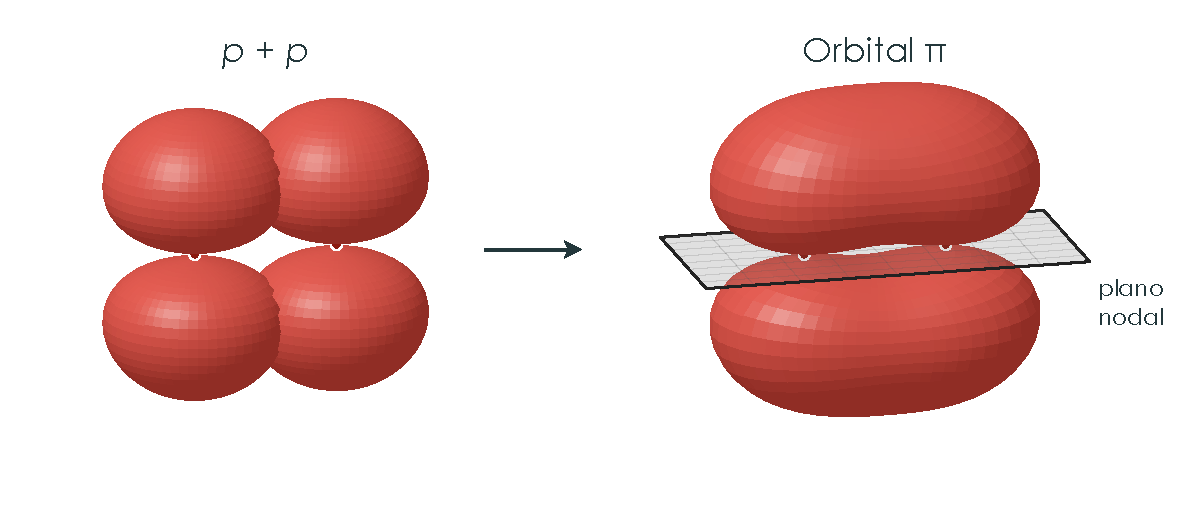
\includegraphics[width=0.75\linewidth]{FigurasSVG/UD3_Enlace_Quimico/pdf/UD3_31_enlace_pi.pdf}
        \caption{Enlace pi}
        \label{fig:enlacepi}
    \end{figure}
\end{enumerate}

Como ejemplos más representativos podemos mencionar:

\begin{enumerate}[label=\numberballmDarkTeal]

        \item \negrita{\ch{H2}}: en este caso, tenemos un solo enlace \(\sigma\) entre los orbitales \(s\) del hidrógeno.

        \begin{figure}[H]
            \centering
            % [FIGURA ORIGINAL] \includegraphics[scale=0.5]{images/imagesUD3EnlaceQuimico/UD3_Teoria/h2tev}
            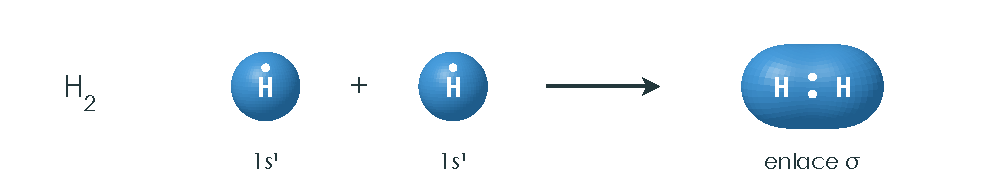
\includegraphics[width=0.7\linewidth]{FigurasSVG/UD3_Enlace_Quimico/pdf/UD3_32_H2_TEV_orbitales.pdf}
            % [FIGURA ORIGINAL] \includegraphics[scale=0.5]{images/imagesUD3EnlaceQuimico/UD3_Teoria/H2tev2}
            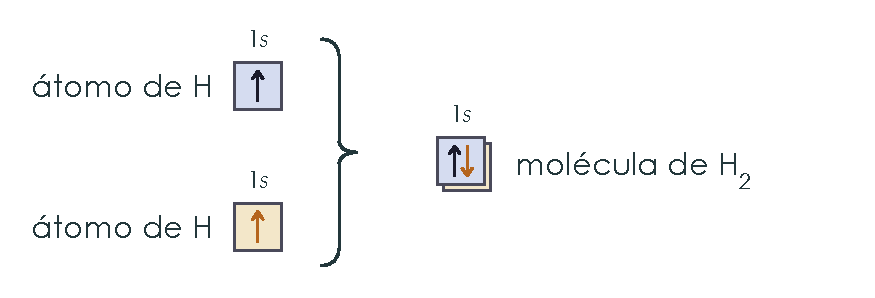
\includegraphics[width=0.55\linewidth]{FigurasSVG/UD3_Enlace_Quimico/pdf/UD3_33_H2_TEV_cajas.pdf}
            \caption{Enlace de \ch{H2} según TEV}
            \label{fig:h2tev}
        \end{figure}

        \item \negrita{\ch{HF}}: en este caso tenemos un enlace \(\sigma\) entre un orbital \(s\) del hidrógeno y un orbital \(p\) del flúor.

        \begin{figure}[H]
            \centering
            % [FIGURA ORIGINAL] \includegraphics[scale=0.5]{images/imagesUD3EnlaceQuimico/UD3_Teoria/HFtev}
            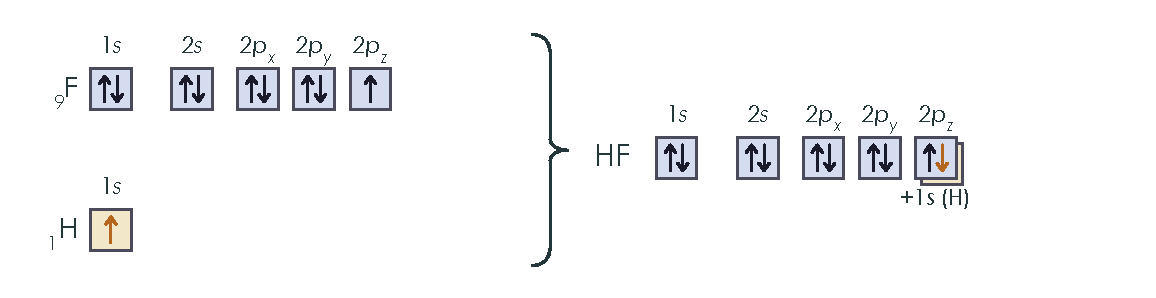
\includegraphics[width=0.75\linewidth]{FigurasSVG/UD3_Enlace_Quimico/pdf/UD3_34_HF_TEV_cajas.pdf}
            \caption{Enlace de \ch{HF} según TEV}
            \label{fig:hftev}
        \end{figure}
        \item \negrita{\ch{H2O}}: en este caso tenemos dos enlaces \(\sigma\) entre un orbital \(p\) del oxígeno y el orbital \(s\) del hidrógeno.
        \begin{figure}[H]
            \centering
            % [FIGURA ORIGINAL] \includegraphics[scale=0.5]{images/imagesUD3EnlaceQuimico/UD3_Teoria/H2Otev}
            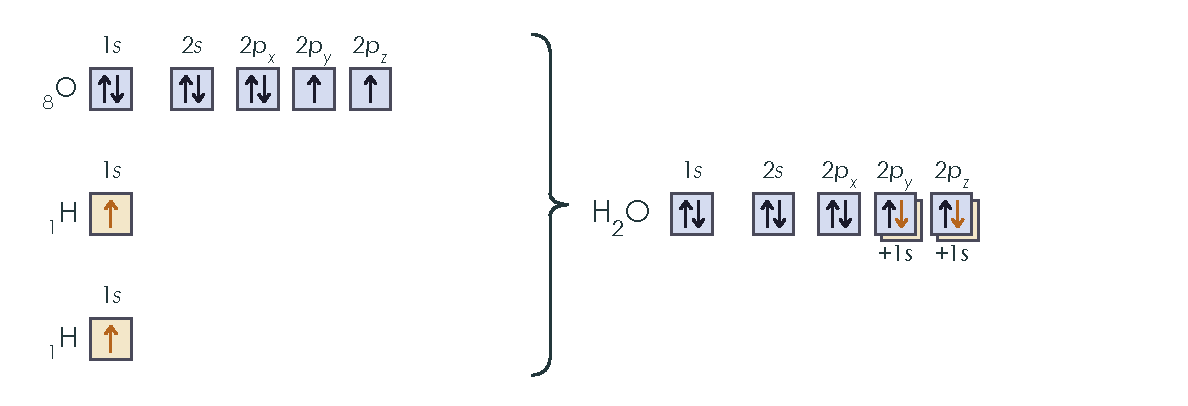
\includegraphics[width=0.75\linewidth]{FigurasSVG/UD3_Enlace_Quimico/pdf/UD3_35_H2O_TEV_cajas.pdf}
            \caption{Enlace de \ch{H2O} según TEV}
            \label{fig:h2otev}
        \end{figure}
        \item \negrita{\ch{O2}}: este es un caso más complejo, en el que tenemos un enlace \(\sigma\) entre un orbital \(p\) de cada átomo de oxígeno y un enlace \(\pi\) entre otro orbital \(p\) de cada átomo de oxígeno.
        \begin{figure}[H]
            \centering
            % [FIGURA ORIGINAL] \includegraphics[scale=0.5]{images/imagesUD3EnlaceQuimico/UD3_Teoria/o2tev}
            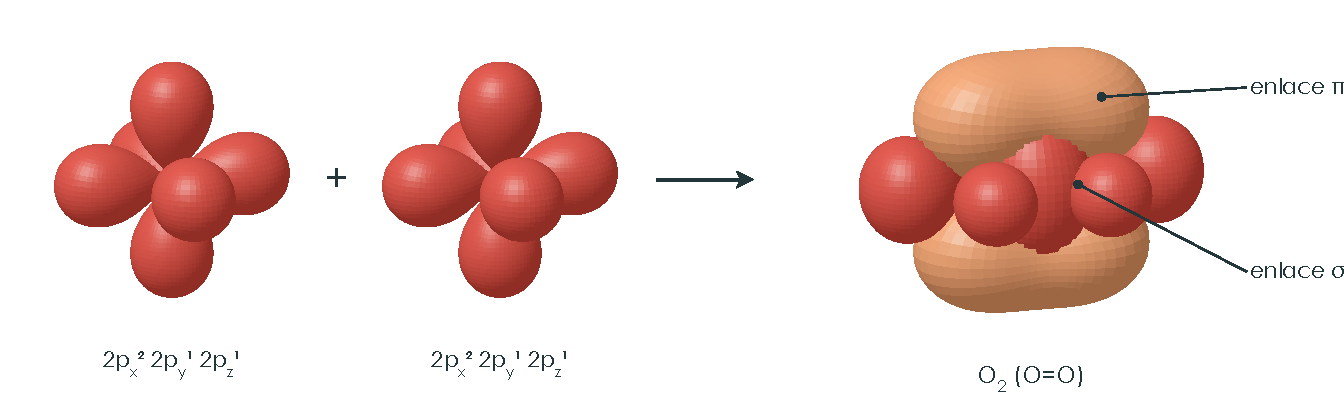
\includegraphics[width=0.85\linewidth]{FigurasSVG/UD3_Enlace_Quimico/pdf/UD3_36_O2_TEV_orbitales.pdf}
            \caption{Enlace de \ch{O2} según TEV}
            \label{fig:o2tev}
        \end{figure}

        Sabemos también que existen moléculas que pueden formar cuatro e incluso 6 enlaces covalentes (\ch{SO2}, \ch{SO3}, \ch{H2SO4}, \ch{SF6}). Estos enlaces los explicaba la teoría de Lewis con las excepciones del octeto expandido.
        Para explicarlo según la teoría del enlace de valencia, tenemos que tener en cuenta que a partir del tercer periodo existen orbitales $d$ que pueden estar vacíos y por tanto se puede producir una expansión de uno de los electrones a estos orbitales, tal y como se muestra en la siguiente figura.
        \begin{figure}[H]
            \centering
            % [FIGURA ORIGINAL] \includegraphics[scale=0.5]{images/imagesUD3EnlaceQuimico/UD3_Teoria/soctetotev}
            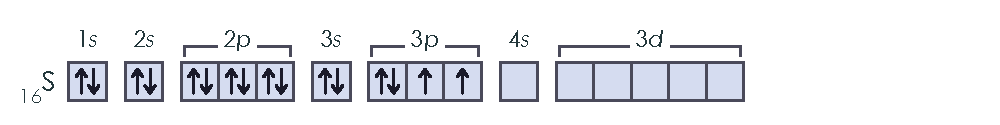
\includegraphics[width=0.75\linewidth]{FigurasSVG/UD3_Enlace_Quimico/pdf/UD3_37_S_covalencia_2.pdf}
            % [FIGURA ORIGINAL] \includegraphics[scale=0.5]{images/imagesUD3EnlaceQuimico/UD3_Teoria/soctetotev2}
            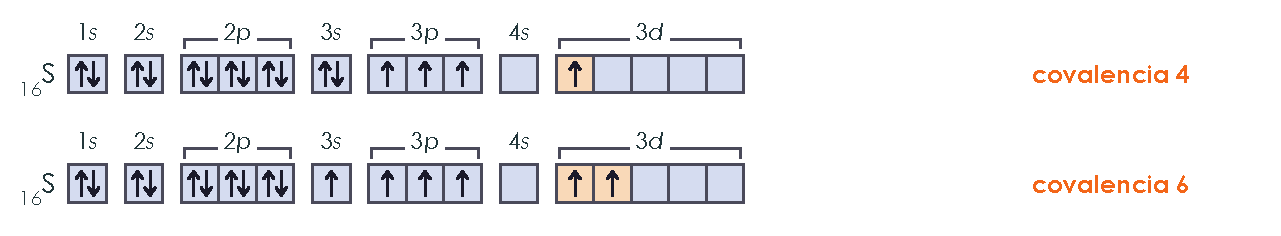
\includegraphics[width=0.85\linewidth]{FigurasSVG/UD3_Enlace_Quimico/pdf/UD3_38_S_covalencias_4_6.pdf}
            \caption{Octeto ampliado según TEV}
            \label{fig:soctetotev}
        \end{figure}
\end{enumerate}

\subsection{Teoría de los orbitales híbridos atómicos}\label{subsec:teoria-de-los-orbitales-hibridos-atomicos}

La TRPECV no puede explicar la geometría de todas las moléculas, del mismo modo que tampoco la teoría del enlace de valencia podía explicar los ángulos de enlace de algunas moléculas.
La \azuln{teoría de hibridación de orbitales atómicos} resolvía estas cuestiones en la que se propuso que durante la reacción y previa formación del enlace, se produce la hibridación o combinación de los orbitales atómicos puros dando lugar a unos nuevos orbitales híbridos.

\subsubsection{Hibridación: concepto y tipos}

\begin{center}
    \begin{definition}[Hibridación]
        La \textbf{hibridación} es un proceso mediante el cual orbitales atómicos puros de energía parecida se combinan entre sí, transformándose en otros orbitales denominados \textbf{orbitales atómicos híbridos}.
    \end{definition}
\end{center}


Los orbitales híbridos se caracterizan por:
\begin{enumerate}[label=\numberballmDarkTeal]
        \item Se forman tantos orbitales híbridos como orbitales atómicos combinados.
        \item Los orbitales híbridos son iguales energéticamente y solo se diferencian en su distribución espacial.
        \item Se disponen en direcciones que facilitan el solapamiento con los orbitales del otro átomo al formar el enlace.
\end{enumerate}

Los tipos de hibridación que nos podemos encontrar son:

\begin{enumerate}[label=\numberballmDarkBrown]
        \item \negsubro{Hibridación $\bm{sp^3}$}.
        Tomaremos como ejemplo el metano \ch{CH4}.
        En este caso los orbitales atómicos que se hibridan son los del carbono.
        El carbono tiene una configuración electrónica: \ch{C}: $\color{blue}{1s^2\;2s^2\;2p_x^1\;2p_y^1\;2p_z^0}$.
        Vemos que uno de los electrones del $2s$ puede promocionar al orbital $2p_z$ vacío quedando una configuración del carbono excitado (se ha producido la promoción de un electrón) \ch{C^*}: $\color{red}{1s^2\;2s^1\;2p_x^1\;2p_y^1\;2p_z^1}$.
        A partir de la combinación de un orbital $s$ (en este caso $2s$) y 3 orbitales $p$ (en este caso $2p$) resultan cuatro orbitales $sp^3$ con una disposición \azuln{tetraédrica} y ángulos de enlace de \rojon{\ang{109.5}}.
        Una vez producida la hibridación del átomo de carbono, se produce el acoplamiento \azuln{frontal} del orbital $s$ del hidrógeno con cada uno de los orbitales $sp^3$ del carbono.
        \begin{figure}[H]
            \centering
            % [FIGURA ORIGINAL] \includegraphics[scale=0.5]{images/imagesUD3EnlaceQuimico/UD3_Teoria/metanosp3}
            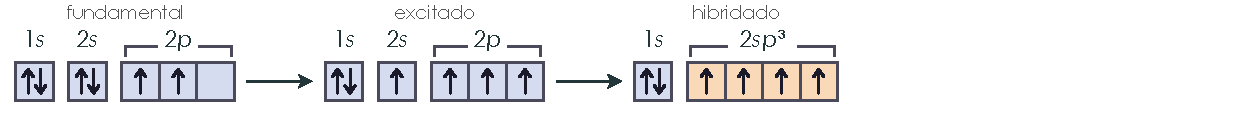
\includegraphics[width=0.85\linewidth]{FigurasSVG/UD3_Enlace_Quimico/pdf/UD3_39_CH4_sp3_cajas.pdf}
            % [FIGURA ORIGINAL] \includegraphics[scale=0.5]{images/imagesUD3EnlaceQuimico/UD3_Teoria/metanosp3_e}
            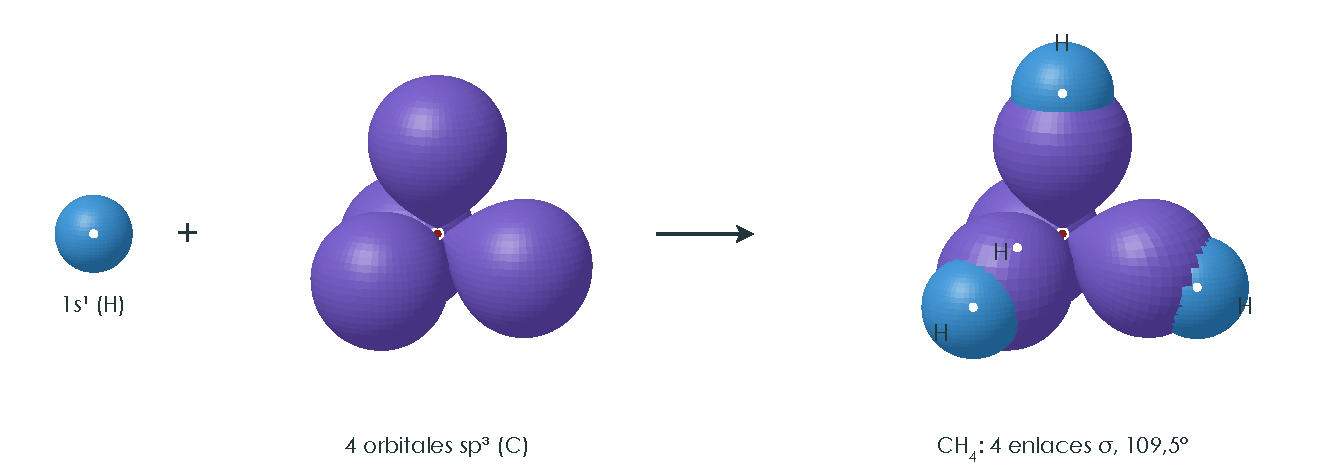
\includegraphics[width=0.85\linewidth]{FigurasSVG/UD3_Enlace_Quimico/pdf/UD3_40_CH4_sp3_orbitales.pdf}
            \caption{Formación del \ch{CH4}}
            \label{fig:formacionmetano}
        \end{figure}

        Cuando se combinen dos orbitales $sp^3$ o un orbital $s$ con un orbital $sp^3$ se forma un enlace de tipo $\sigma$ debido a que se produce un acoplamiento frontal.

        \item \negsubro{Hibridación $\bm{sp^2}$}.
        Tomaremos como ejemplo el \ch{BF3}.
        En este caso los orbitales atómicos que se hibridan son los del boro.
        El boro tiene una configuración electrónica: \ch{B}: $\color{blue}{1s^2\;2s^2\;2p_x^1\;2p_y^0\;2p_z^0}$.
        Vemos que \azuln{uno}  de los electrones del $2s$ puede promocionar al orbital $2p_y$ vacío quedando una configuración del boro excitado (se ha producido la promoción de un electrón) \ch{B^*}: $\color{red}{1s^2\;2s^1\;2p_x^1\;2p_y^1\;2p_z^0}$.
        A partir de la combinación de un orbital $s$ (en este caso $2s$) y 2 orbitales $p$ (en este caso $2p_x$ y $2p_y$ ) resultan tres orbitales $sp^2$ con una disposición \azuln{trigonal plana} y ángulos de enlace de \rojon{\ang{120}}.
        Una vez producida la hibridación del átomo de boro, se produce el acoplamiento \azuln{frontal} del orbital $p$ del flúor con cada uno de los orbitales $sp^2$ del boro.
        \begin{figure}[H]
            \centering
            % [FIGURA ORIGINAL] \includegraphics[scale=0.75]{images/imagesUD3EnlaceQuimico/UD3_Teoria/BF3sp2}
            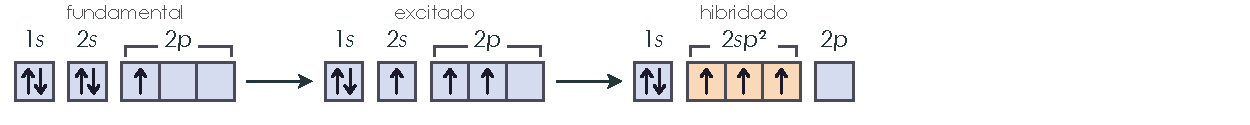
\includegraphics[width=0.85\linewidth]{FigurasSVG/UD3_Enlace_Quimico/pdf/UD3_41_BF3_sp2_cajas.pdf}
            \caption{Formación del \ch{BF3}}
            \label{fig:formacionbf3}
        \end{figure}
        Otro ejemplo sería la formación del \ch{AlCl3}.
        En este caso se hibridaría el átomo de aluminio según:
        \begin{figure}[H]
            \centering
            % [FIGURA ORIGINAL] \includegraphics[scale=0.75]{images/imagesUD3EnlaceQuimico/UD3_Teoria/AlCl3sp2}
            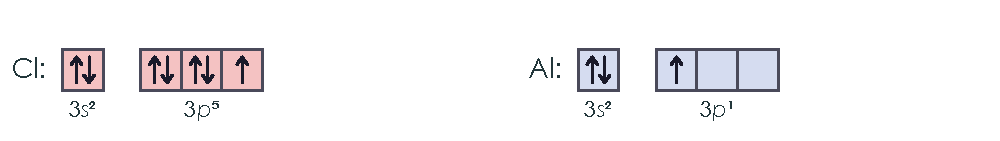
\includegraphics[width=0.7\linewidth]{FigurasSVG/UD3_Enlace_Quimico/pdf/UD3_42_AlCl3_cajas_fundamental.pdf}
            % [FIGURA ORIGINAL] \includegraphics[scale=0.75]{
            % [FIGURA ORIGINAL] images/imagesUD3EnlaceQuimico/UD3_Teoria/AlCl3sp2_b}
            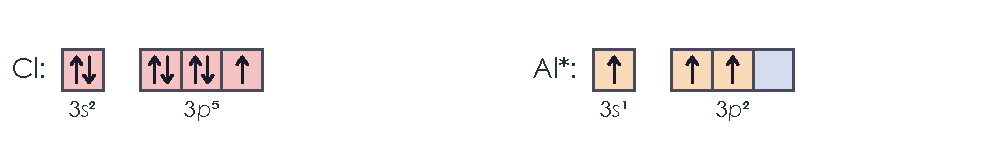
\includegraphics[width=0.7\linewidth]{FigurasSVG/UD3_Enlace_Quimico/pdf/UD3_43_AlCl3_cajas_excitado.pdf}
            \caption{Formación del \ch{AlCl3}}
            \label{fig:formacionalcl3}
        \end{figure}
        En este caso el orbital $3s$ se combina con dos orbitales $2p$ para formar tres orbitales híbridos $sp^2$.
        Estos orbitales híbridos del aluminio se combinarán en este caso con orbitales $p$ del cloro para formar la molécula de \ch{AlCl3}
        \begin{figure}[H]
            \centering
            % [FIGURA ORIGINAL] \includegraphics[scale=0.75]{images/imagesUD3EnlaceQuimico/UD3_Teoria/AlCl3sp2_c}
            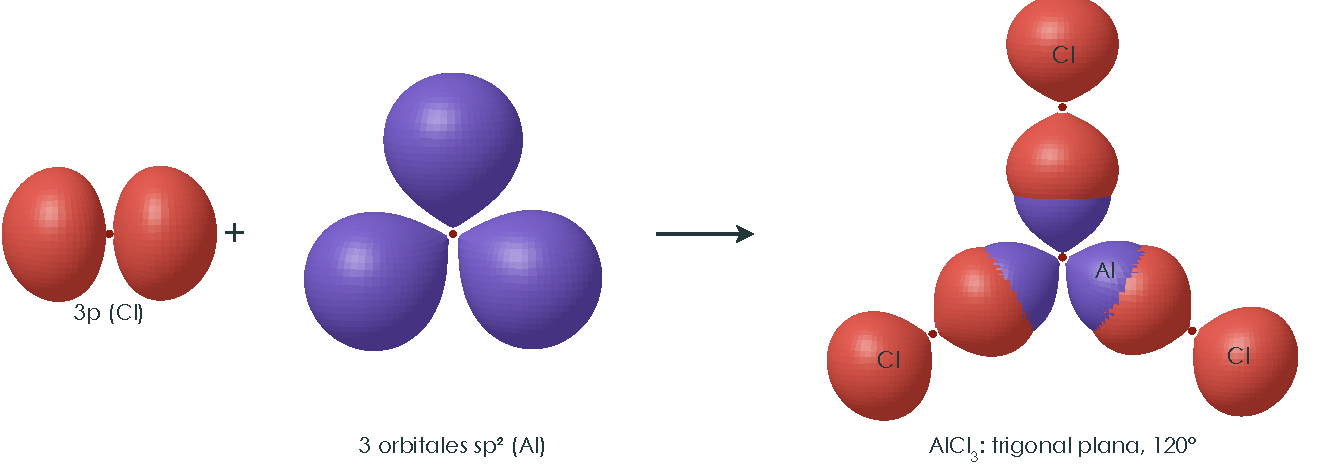
\includegraphics[width=0.85\linewidth]{FigurasSVG/UD3_Enlace_Quimico/pdf/UD3_44_AlCl3_sp2_orbitales.pdf}
            \caption{Formación del \ch{AlCl3}}
            \label{fig:formacionalcl3_b}
        \end{figure}

        \item \negsubro{Hibridación $\bm{sp}$}.
        Tomaremos como ejemplo el \ch{BeF2}.
        En este caso los orbitales atómicos que se hibridan son los del berilio.
        El berilio tiene una configuración electrónica: \ch{Be}: $\color{blue}{1s^2\;2s^2\;2p_x^0\;2p_y^0\;2p_z^0}$.
        Vemos que \azuln{uno} de los electrones del $2s$ puede promocionar al orbital $2p_x$ vacío quedando una configuración del berilio excitado (se ha producido la promoción de un electrón) \ch{Be^*}: $\color{red}{1s^2\;2s^1\;2p_x^1\;2p_y^0\;2p_z^0}$.

        \begin{figure}[H]
            \centering
            % [FIGURA ORIGINAL] \includegraphics[scale=0.5]{images/imagesUD3EnlaceQuimico/UD3_Teoria/BeF2sp}
            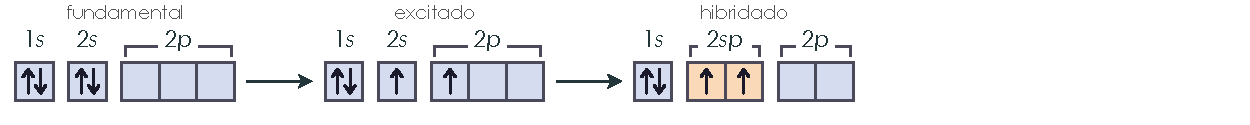
\includegraphics[width=0.85\linewidth]{FigurasSVG/UD3_Enlace_Quimico/pdf/UD3_45_BeF2_sp_cajas.pdf}
            % [FIGURA ORIGINAL] \includegraphics[scale=0.5]{images/imagesUD3EnlaceQuimico/UD3_Teoria/BeF2sp_b}
            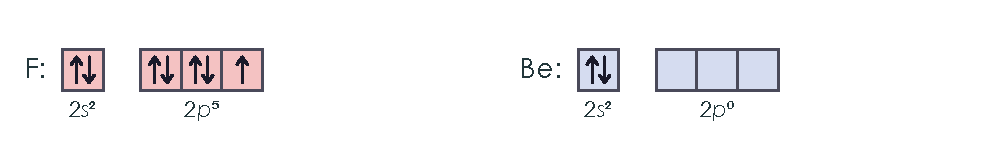
\includegraphics[width=0.7\linewidth]{FigurasSVG/UD3_Enlace_Quimico/pdf/UD3_46_BeF2_cajas_fundamental.pdf}
            % [FIGURA ORIGINAL] \includegraphics[scale=0.5]{images/imagesUD3EnlaceQuimico/UD3_Teoria/BeF2sp_c}
            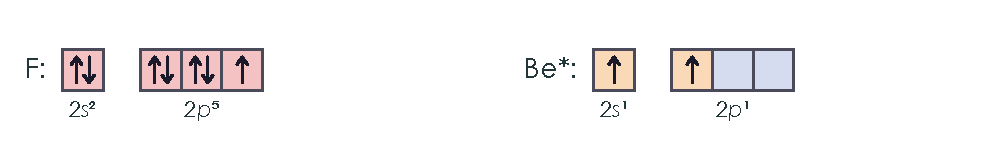
\includegraphics[width=0.7\linewidth]{FigurasSVG/UD3_Enlace_Quimico/pdf/UD3_47_BeF2_cajas_excitado.pdf}
            \caption{Formación del \ch{BeF2}}
            \label{fig:formacionbef2}
        \end{figure}

        A partir de la combinación de un orbital $s$ (en este caso $2s$) y 1 orbital $p$ (en este caso $2p_x$) resultan dos orbitales $sp$ con una disposición \azuln{lineal} y ángulos de enlace de \rojon{\ang{180}}.
        Una vez producida la hibridación del átomo de berilio, se produce el acoplamiento \azuln{frontal} del orbital $p$ del flúor con cada uno de los orbitales $sp$ del berilio.

        \begin{figure}[H]
            \centering
            % [FIGURA ORIGINAL] \includegraphics[scale=0.5]{images/imagesUD3EnlaceQuimico/UD3_Teoria/BeF2sp_d}
            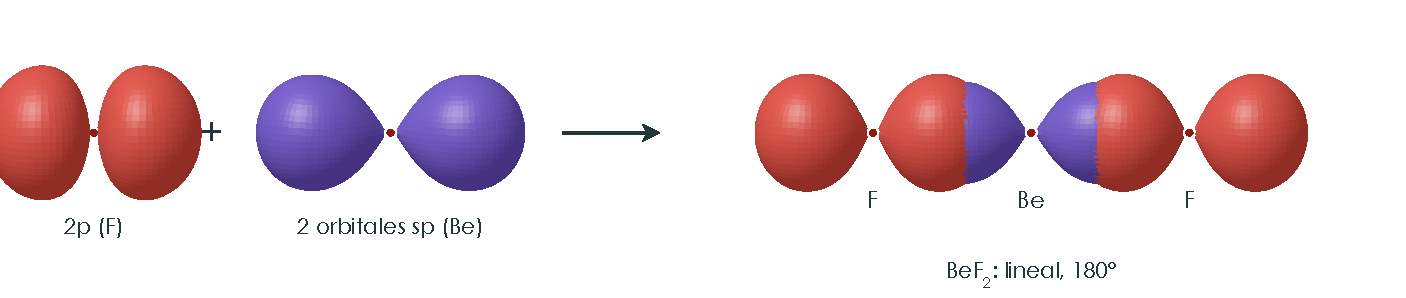
\includegraphics[width=0.85\linewidth]{FigurasSVG/UD3_Enlace_Quimico/pdf/UD3_48_BeF2_sp_orbitales.pdf}
            \caption{Formación del \ch{BeF2}}
            \label{fig:formacionBeF2_b}
        \end{figure}

        \item \negsubro{Hibridación $dsp^2$}.
        A partir de un orbital $d$, un orbital $s$ y dos orbitales $p$ resultan cuatro orbitales de un mismo plano formando ángulos \rojon{\ang{90}} entre sí.
        Ejemplos: \ch{Ni(CO)4}

        \item \negsubro{Hibridación $d^2sp^3$}.
        A partir de dos orbitales $d$, un orbital $s$ y tres orbitales $p$ dan lugar a 6 orbitales híbridos $d^2sp^3$.
        Forma una geometría \azuln{octaédrica} con ángulos de enlace \rojon{\ang{90}}.
        Ejemplo: \ch{SF6}.
        \item \negsubro{Hibridación $dsp^3$}.
        A partir de 1 orbital $d$, un orbital $s$ y tres orbitales $p$ dan lugar a 5 orbitales híbridos $dsp^3$.
        Forma una geometría \azuln{bipirámide trigonal} con ángulos de enlace de \rojon{\ang{120}} y \rojon{\ang{90}}.
        Ejemplo: \ch{PCl5}
\end{enumerate}

\subsubsection{Tipos de enlaces entre los orbitales cuando se produce hibridaciones}
Cuando tenemos hibridaciones los enlaces $\sigma$ y enlaces $\pi$ se producen por el acoplamiento de los siguientes tipos de orbitales:
\begin{enumerate}[label=\numberballmDarkTeal]
        \item \negsubro{Enlace $\sigma$}.
        Tendremos un acoplamiento frontal
        \begin{enumerate}
            \item Orbital híbrido -- orbital híbrido siempre y cuando sean del mismo tipo
            \item Cualquier orbital híbrido -- s
            \item Cualquier orbital híbrido -- p
        \end{enumerate}
        \item \negsubro{Enlace $\pi$}.
        Tendremos un acoplamiento lateral.
        Y se produce por acoplamiento de cualquier orbital $p$ siempre y cuando se produzca de manera transversal.
\end{enumerate}

\marcador{Ejercicio}: Explicar los enlaces de las moléculas de \azuln{etano}, \azuln{eteno} y \azuln{etino}

\subsection{Teoría de los orbitales moleculares (OOMM)}\label{subsec:teoria-de-los-orbitales-moleculares-(oomm)}

Un orbital molecular es una zona en la que es probable que se encuentre un determinado electrón.

Los orbitales moleculares se forman por combinaciones lineales de orbitales atómicos.
La combinación de $\bm{n}$ orbitales atómicos producen la formación de $\bm{2n}$ orbitales moleculares teniendo siempre un orbital molecular \azuln{enlazante} (máxima probabilidad de encontrar los electrones) y un orbital molecular \azuln{antienlazante} (mínima probabilidad de encontrar los electrones.).
Los orbitales moleculares se representan mediante su correspondiente función de onda ($\Psi$)
\begin{gather}
    \text{\textbf{Orbital molecular enlazante: }}\quad \Psi_{enlazante} = c_1\Psi_A + c_2\Psi_B\separ
    \text{\textbf{Orbital molecular antienlazante: }}\quad \Psi_{antienlazante} = c_1\Psi_A - c_2\Psi_B
\end{gather}

\subsubsection{Tipos de orbitales moleculares}

Los orbitales moleculares los podemos resumir en dos tipos $\sigma$ y tipo $\pi$
\begin{enumerate}[label=\numberballmDarkTeal]
        \item \negsubro{Orbitales $\sigma$}.
        Se obtienen por interacción frontal de forma similar a lo visto anteriormente y cuando se forman siempre tendremos orbitales $\sigma$ enlazantes representados por $\sigma$ y orbitales $\sigma$ antienlazantes representados por $\sigma^*$.
        \item \negsubro{Orbitales $\pi$}.
        Se obtienen por interacción lateral de forma similar a lo visto anteriormente y cuando se forman siempre tendremos orbitales $\pi$ enlazantes representados por $\pi$ y orbitales $\pi$ antienlazantes representados por $\pi^*$.
\end{enumerate}

\begin{figure}[h]
    \centering
    % [FIGURA ORIGINAL] \includegraphics[scale=0.5]{images/imagesUD3EnlaceQuimico/UD3_Teoria/orbitales_moleculares}
    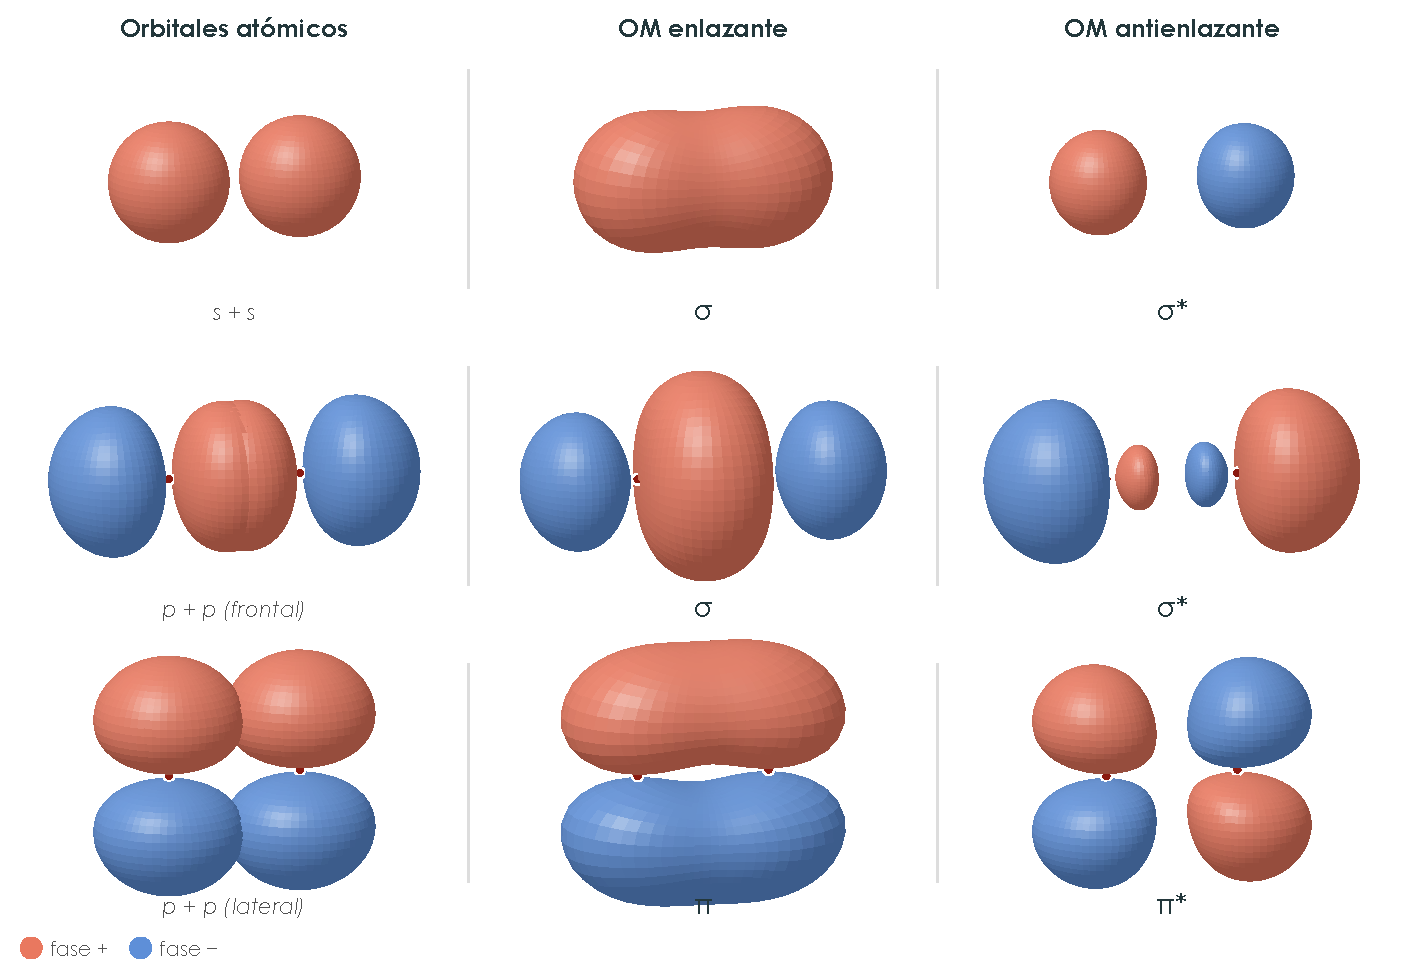
\includegraphics[width=0.85\linewidth]{FigurasSVG/UD3_Enlace_Quimico/pdf/UD3_49_orbitales_moleculares.pdf}
    \caption{(a) Orbitales moleculares $\sigma$ enlazantes y antienlazantes formados a partir de orbitales atómicos $s$ y $p$. (b) orbitales moleculares $\pi$ enlazantes y antienlazantes formados a partir de orbitales atómicos $p$ y $d$}
    \label{fig:Orbitalesatomicos}
\end{figure}

%    \subsection{Diagramas de energía y configuración electrónica}\label{subsec:diagramas-de-energia-y-configuracion-electronica}
%
%    En el caso de moléculas formadas por dos átomos iguales, el orden creciente de energías es, para los dos primeros niveles el siguiente:
%    \begin{figure}[H]
%        \centering
%        \includegraphics[scale=0.5]{images/imagesUD3EnlaceQuimico/UD3_Teoria/diagrama_energia_oomm}
%        \caption{Origen energético moléculas homoatómicas}
%        \label{fig:orgenenergeticooomm}
%    \end{figure}
%
%    A continuación, se muestra el diagrama energético para las moléculas de \ch{H2} y de \ch{O2}.
%
%    \begin{figure}[h]
%        \centering
%        \includegraphics[scale=0.5]{images/imagesUD3EnlaceQuimico/UD3_Teoria/diagrama_oomm_h2}
%        \caption{Diagrama energético OOMM para el \ch{H2}}
%        \includegraphics[scale=0.5]{images/imagesUD3EnlaceQuimico/UD3_Teoria/diagrama_oomm_o2}
%        \caption{Diagrama energético OOMM para el \ch{O2}}
%        \label{fig:Diagramaoommh2yo2}
%    \end{figure}

% \subsection{Propiedades de los compuestos covalentes}

% A diferencia de las sustancias iónicas, las sustancias iónicas tendrán un tipo de propiedades según se enlacen como moléculas discretas o formen redes tridimensionales.

% \begin{enumerate}[label=\numberballmDarkTeal]
%     \item \negsubro{Sustancias moleculares}. Suelen ser moléculas discretas pero que en determinadas ocasiones y en las condiciones ópticas de presión y temperatura pueden formar \azuln{cristales moleculares}
%           \begin{enumerate}
%               \item \negrita{Estado de agregación}. Tienen baja densidad, suelen ser gases o líquidos de bajo punto de ebullición o en algunos casos sólidos blandos de bajo punto de fusión y subliman fácilmente.
%               \item \negrita{Solubilidad}. Dependerá de las fuerzas intermoleculares (se verá más adelante). Las sustancias polares se disolverán en disolventes polares y las sustancias apolares en sustancias apolares (\textit{lo semejante disuelve a lo semejante})
%               \item \negrita{Conductividad eléctrica}. No conducen la electricidad, son buenos \azuln{aislantes}
%           \end{enumerate}
%     \item \negsubro{Sustancias atómicas}. Son sustancias que se agrupan de manera que forman redes moleculares similares a las redes cristalinas de los compuestos iónicos. Ejemplos: grafito, \ch{SiO2}
%           \begin{enumerate}
%               \item \negrita{Estado de agregación}. Suelen ser sólidos de alto punto de fusión y ebullición.
%               \item \negrita{Solubilidad}. Suelen ser insolubles en cualquier disolvente
%               \item \negrita{Conductividad eléctrica}. Son malos conductores de la electricidad con la excepción del grafito.
%           \end{enumerate}
% \end{enumerate}

\subsection{Sólidos covalentes}\label{subsec:solidos-covalentes}

Hay sustancias sólidas formadas por un número indeterminado de átomos unidos mediante un enlace covalente.
Se llaman \textbf{sólidos covalentes}.

Los sólidos covalentes más comunes son el diamante, grafito y la sílice

\begin{enumerate}[label=\numberballmDarkTeal]
        \item El \textbf{diamante} está formado por átomos de carbono con hibridación \(\bm{sp^3}\).
        Cada átomo de carbono está unido a otros cuatro átomos mediante enlaces covalentes.
        Es el material más duro que existe teniendo por tanto también un elevado \textbf{punto de fusión}.
        \begin{figure}[H]
            \centering
            % [FIGURA ORIGINAL] \includegraphics[scale=0.2]{images/imagesUD3EnlaceQuimico/UD3_Teoria/diamante}
            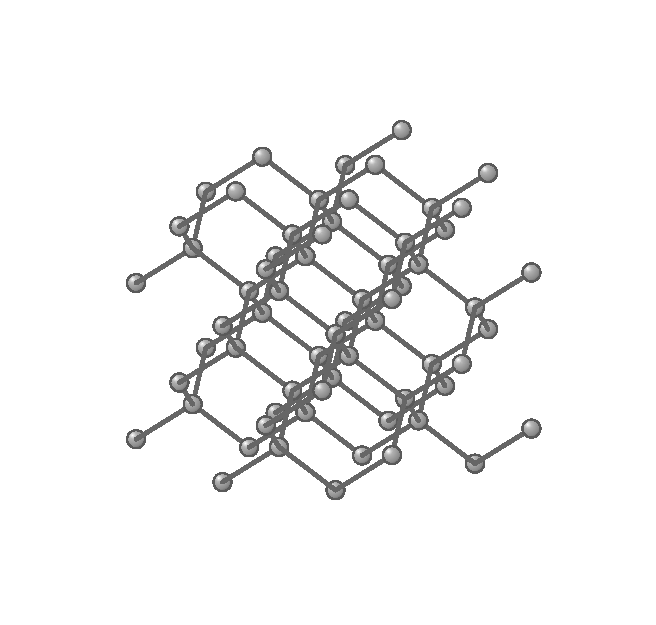
\includegraphics[width=0.45\linewidth]{FigurasSVG/UD3_Enlace_Quimico/pdf/UD3_50_diamante.pdf}
            \caption{Estructura atómica del diamante}\label{fig:diamante}
        \end{figure}
        \item El \textbf{grafito} está formado por carbono con una hibridación \(\bm{sp^2}\).
        Forma anillos planos con una geometría trigonal plana.
        Los electrones que están en los orbitales \(\bm{p}\) perpendiculares al plano forman una nube \(\bm{\pi}\) que permite la conductividad eléctrica.

        \begin{figure}[H]
            \centering
            % [FIGURA ORIGINAL] \includegraphics[scale=1.6]{images/imagesUD3EnlaceQuimico/UD3_Teoria/grafitob}
            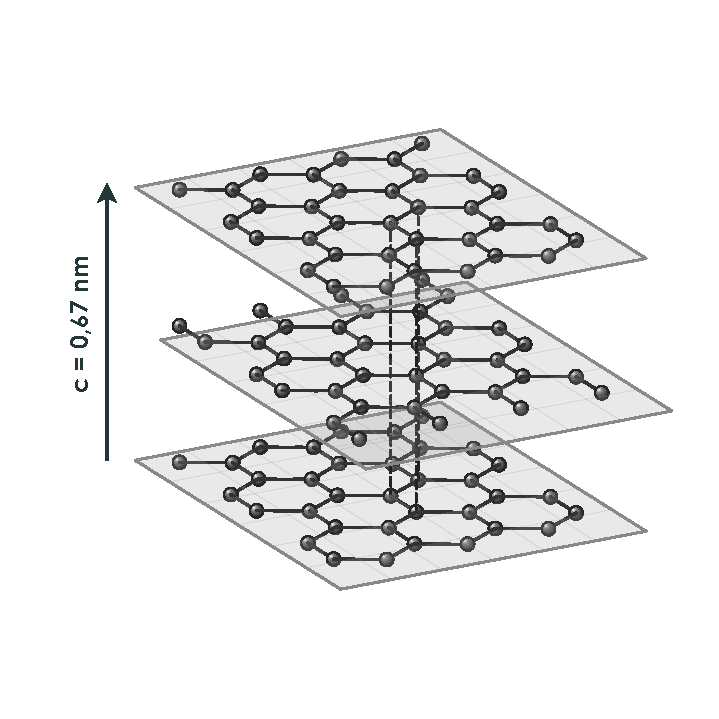
\includegraphics[width=0.45\linewidth]{FigurasSVG/UD3_Enlace_Quimico/pdf/UD3_51_grafito.pdf}
            \caption{Estructura atómica del grafito}
            \label{fig:grafito}
        \end{figure}

        \item La sílice (\ch{SiO2}) es un material muy duro formado por átomos de Si con una estructura tetraédrica en la que en cada extremo hay un átomo de oxígeno.
        La arena de la playa y el cuarzo son de sílice.
\end{enumerate}

\subsection{Propiedades de los compuestos covalentes}\label{subsec:propiedades-de-los-compuestos-covalentes}

A diferencia de las sustancias iónicas, las sustancias covalentes tendrán un tipo de propiedades según se enlacen como moléculas discretas o formen redes tridimensionales.

\begin{enumerate}[label=\numberballmDarkTeal]
        \item Los \textbf{sólidos covalentes} son sólidos de elevado \textbf{punto de fusión}, ya que, para fundirlos, hay que romper los enlaces covalentes que existen entre los átomos.
        \item Las \textbf{sustancias covalentes moleculares}  se pueden presentar a temperatura ambiente como sólidos, líquidos o gases dependiendo del tipo de fuerzas intermoleculares (se verán en el siguiente apartado) que presenten.
        En cualquier caso, estos compuestos presentan puntos de fusión y ebullición inferiores a los de los compuestos iónicos y metálicos.
        \item Las sustancias covalentes moleculares son \textbf{solubles en disolventes de polaridad similar}.
        Por ejemplo una sustancia polar como el etanol, se disuelve en disolventes polares como el agua o una sustancia apolar como las grasas se disuelven en disolventes apolares como el hexano.
        \item Las sustancias covalentes localizadas \textbf{no conducen la electricidad en ningún estado,} pero sí son conductoras de la electricidad sustancias como el grafito que presentan una nube \(\bm{\pi}\) en la que puede existir la movilidad de los electrones.
        \item Las sustancias covalentes son \textbf{blandas y elásticas}.
        \item Los \textbf{sólidos covalentes} son \textbf{duros} y \textbf{frágiles}
\end{enumerate}


\section{Fuerzas intermoleculares}\label{sec:fuerzas-intermoleculares}

\begin{center}
    \begin{definition}[Fuerzas intermoleculares]
        Son aquellas que se producen entre las distintas moléculas y, por tanto, no implica un enlace como tal
    \end{definition}
\end{center}


Las fuerzas intermoleculares serán las que determine finalmente el \textbf{estado de agregación} y los \textbf{puntos de fusión y ebullición} de ese compuesto.
Además, estas fuerzas disminuyen al aumentar la distancia entre las moléculas por lo que es obvio decir que estas fuerzas son menos importantes o prácticamente irrelevantes en los gases, siendo relevantes en los sólidos y los líquidos.

Tenemos principalmente dos tipos de fuerzas:
\begin{enumerate}[label=\numberballmDarkTeal]
        \item \negsubro{Enlaces de hidrógeno}.
        Es un tipo de interacción \textbf{especial} que se da siempre entre un átomo de hidrógeno (\ch{H}) y un átomo electronegativo que suele ser el flúor (\ch{F}), oxígeno (\ch{O}) o nitrógeno (\ch{N}).

        La aparición de una carga parcial positiva ($\delta +$) en el hidrógeno y una carga parcial negativa ($\delta -$) en el átomo de \ch{F}, \ch{N} ó \ch{O} origina una atracción electrostática entre el átomo de hidrógeno de una molécula y el átomo más electronegativo de otra molécula.
        \begin{figure}[H]
            \centering
            % [FIGURA ORIGINAL] \includegraphics[scale=0.4]{images/imagesUD3EnlaceQuimico/UD3_Teoria/puentes_hidrogeno}
            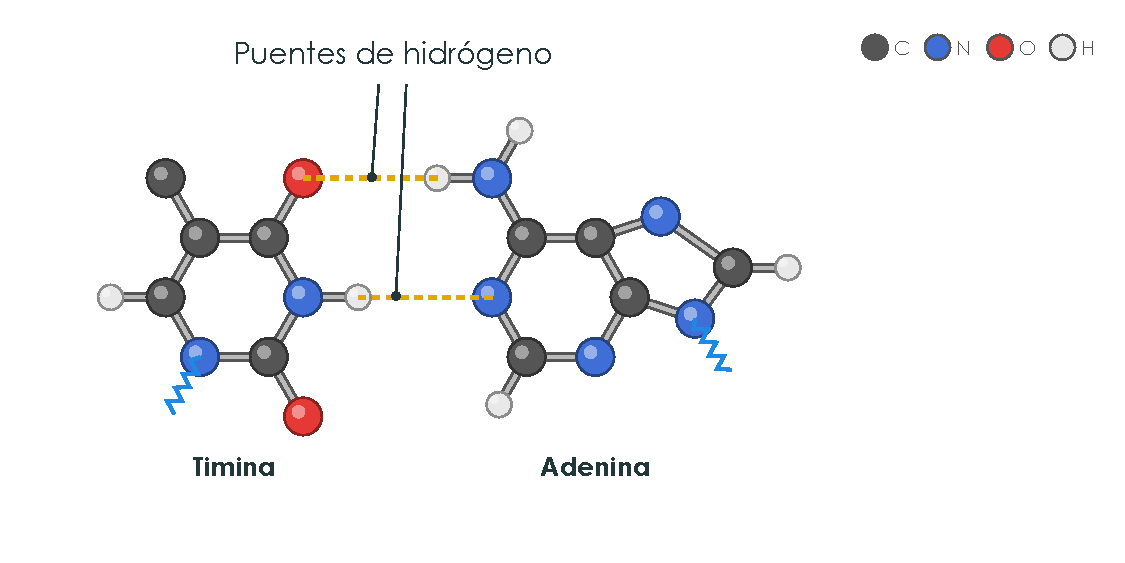
\includegraphics[width=0.6\linewidth]{FigurasSVG/UD3_Enlace_Quimico/pdf/UD3_52_puentes_hidrogeno_ADN.pdf}
            % [FIGURA ORIGINAL] \includegraphics[scale=0.3]{images/imagesUD3EnlaceQuimico/UD3_Teoria/puentes_hidrogeno_b}
            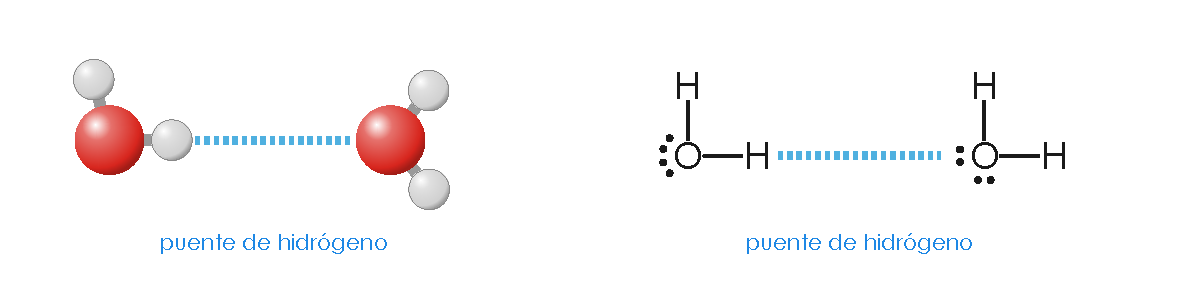
\includegraphics[width=0.6\linewidth]{FigurasSVG/UD3_Enlace_Quimico/pdf/UD3_53_puentes_hidrogeno_agua.pdf}
            \caption{Puentes de hidrógeno en la molécula de \ch{H2O}}\label{fig:puentes-de-hidrogeno}
        \end{figure}
        \begin{figure}[H]
            \centering
            % [FIGURA ORIGINAL] \includegraphics[scale=0.4]{images/imagesUD3EnlaceQuimico/UD3_Teoria/puentes_hidrogeno_c}
            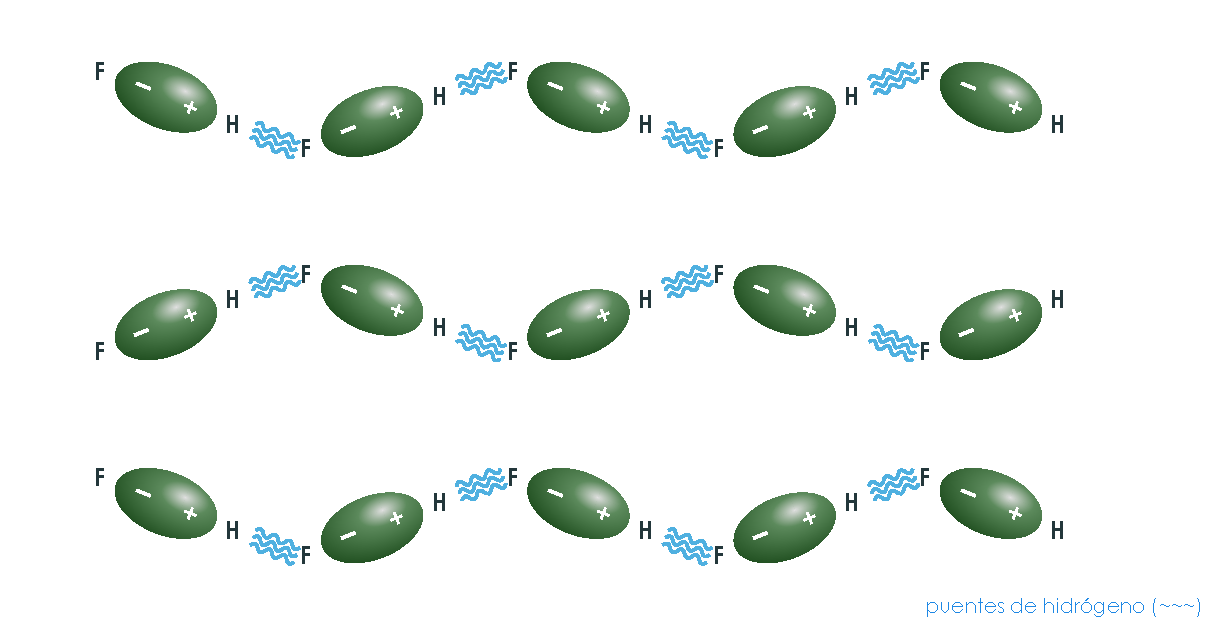
\includegraphics[width=0.6\linewidth]{FigurasSVG/UD3_Enlace_Quimico/pdf/UD3_54_puentes_hidrogeno_HF.pdf}
            \caption{Puentes de hidrógeno en la molécula de \ch{HF}}
            \label{fig:puentesdehidrogeno}
        \end{figure}
        \item \negsubro{Fuerzas de Van der Waals}
        \begin{enumerate}[label=\letraminuscula]
            \item \negrita{Fuerzas de London o dispersión}.
            Se da en moléculas \textbf{apolares}.
            La interacción se produce porque debido a las fluctuaciones de los electrones en la molécula se producen pequeños dipolos.
            \begin{figure}[H]
                \centering
                % [FIGURA ORIGINAL] \includegraphics[scale=0.5]{images/imagesUD3EnlaceQuimico/UD3_Teoria/fuerzaslondon}
                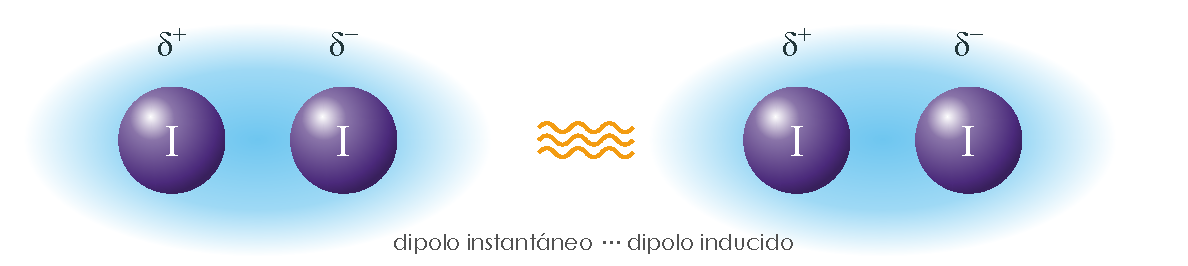
\includegraphics[width=0.6\linewidth]{FigurasSVG/UD3_Enlace_Quimico/pdf/UD3_55_fuerzas_london.pdf}
                \caption{Fuerzas de London en la molécula de \ch{F2}}
                \label{fig:fuerzasdelondon}
            \end{figure}
            \item \negrita{Fuerzas dipolo--dipolo}.
            Se produce entre moléculas \textbf{covalentes polares}.
            \begin{figure}[H]
                \centering
                % [FIGURA ORIGINAL] \includegraphics[scale=0.5]{images/imagesUD3EnlaceQuimico/UD3_Teoria/dipolodipolo}
                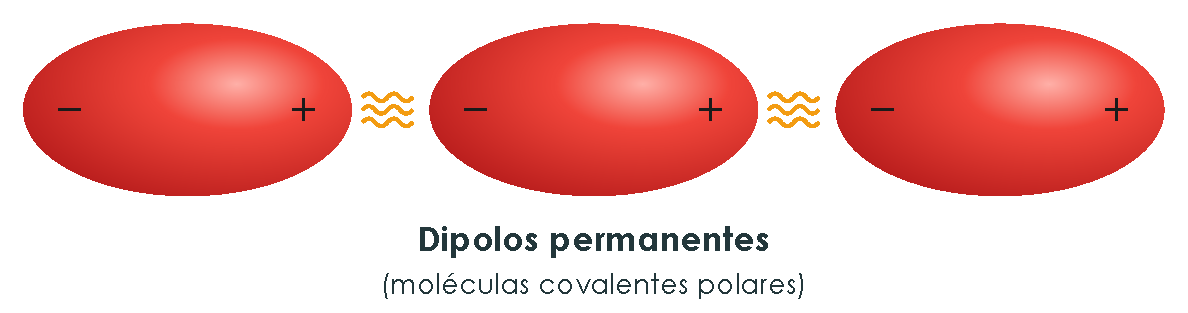
\includegraphics[width=0.6\linewidth]{FigurasSVG/UD3_Enlace_Quimico/pdf/UD3_56_dipolo_dipolo.pdf}
                \caption{Fuerzas dipolo--dipolo en la molécula de \ch{H2S}}
                \label{fig:fuerzasdipolodipolo}
            \end{figure}
            \item \negrita{Fuerzas dipolo--dipolo inducido}.
            Estas fuerzas aparecen cuando mezclamos moléculas \textbf{polares} con \textbf{apolares}, las moléculas polares ya tienen un dipolo y estas inducen la generación de un dipolo en las moléculas apolares (dipolo inducido).
            \begin{figure}[H]
                \centering
                % [FIGURA ORIGINAL] \includegraphics[scale=0.5]{images/imagesUD3EnlaceQuimico/UD3_Teoria/dipolodipoloinducido}
                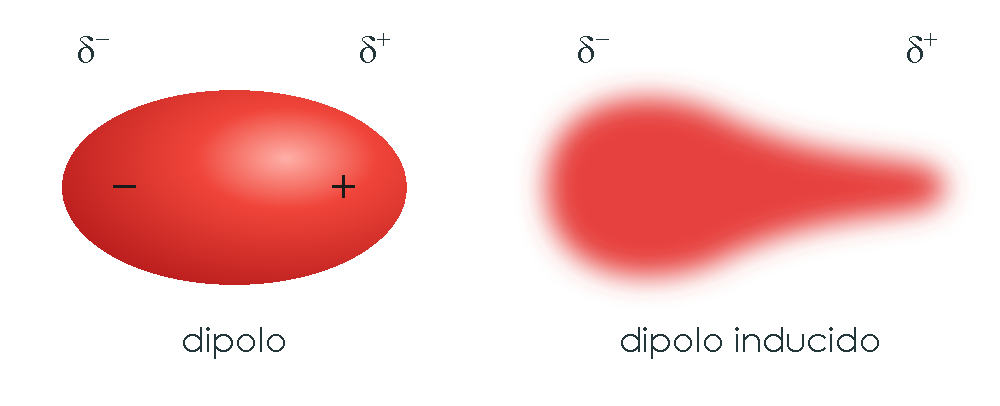
\includegraphics[width=0.55\linewidth]{FigurasSVG/UD3_Enlace_Quimico/pdf/UD3_57_dipolo_dipolo_inducido.pdf}
                \caption{Fuerzas dipolo--dipolo inducido}
                \label{fig:dipolodipoloinducido}
            \end{figure}
        \end{enumerate}
\end{enumerate}

\subsection{Fortaleza de las interacciones intermoleculares}\label{subsec:fortaleza-de-las-interacciones-intermoleculares}

No todos los enlaces intermoleculares presentan la misma fortaleza, el orden creciente en la fortaleza de las fuerzas intermoleculares es:

Enlaces de hidrógeno $>$ Fuerzas dipolo-dipolo $>$ Fuerzas dipolo-dipolo inducido $>$ Fuerzas de London.


\section{Enlace metálico}\label{sec:enlace-metalico}

Los metales constituyen el 80\% de los elementos químicos.
Las teorías para explicar el enlace metálico deben por tanto justificar las distintas propiedades de los metales.
Podemos destacar dos teorías:

\begin{enumerate}[label=\numberballmDarkTeal]
        \item \negsubro{Modelo de la nube electrónica: modelo de Drude}.
        Los cationes metálicos forman una red cristalina en cuyo interior hay una \azuln{nube de electrones} de valencia que se mueven libremente actuando también como unión de los iones positivos.
        La atracción electrostática entre los electrones y cationes mantiene fuertemente unidos a todos los átomos del metal.
        \begin{figure}[H]
            \centering
            % [FIGURA ORIGINAL] \includegraphics[scale=0.5]{images/imagesUD3EnlaceQuimico/UD3_Teoria/enlacemetalico_nubeelectronica}
            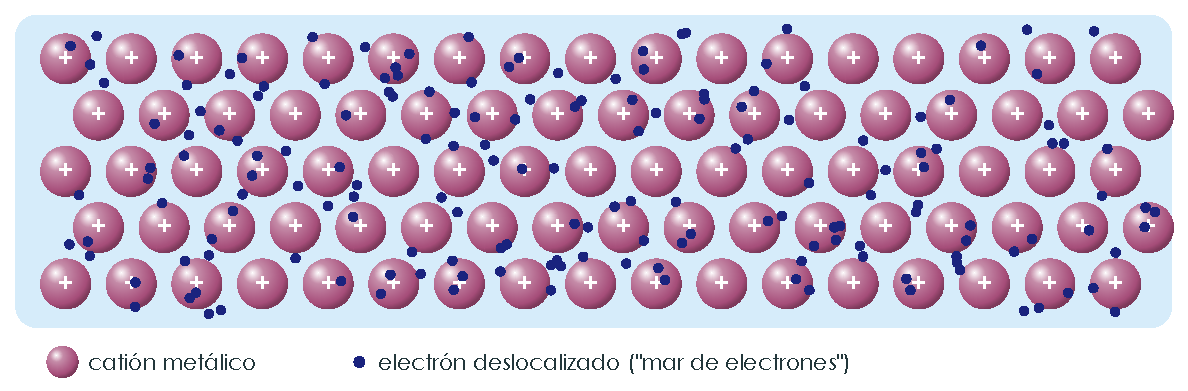
\includegraphics[width=0.8\linewidth]{FigurasSVG/UD3_Enlace_Quimico/pdf/UD3_58_enlace_metalico.pdf}
            \caption{Modelo de la nube electrónica del enlace metálico}
            \label{fig:modelonubeelectronica}
        \end{figure}
        Este modelo explica algunas propiedades de los metales como la conductividad eléctrica, brillo metálico etc., pero no otras como el comportamiento de los semiconductores.
        \item \negsubro{Teoría de bandas}.
        Es un modelo que se basa en el modelo cuántico de la teoría de los OOMM. A medida que aumentamos el número de orbitales atómicos, aumentamos el número de orbitales moleculares y si es lo suficientemente grande los niveles energéticos se suceden dando lugar a \azuln{bandas de energía}.

        \xmybox{\negrita{Teoría de bandas para el \ch{Mg}}}. \ch{Mg} = \elconf{12}.
        El magnesio tiene dos electrones situados en el orbital $3s$, quedando los orbitales $3p$ vacíos.
        Si consideramos el metal como muchos átomos de magnesio juntos, podemos imaginar la aparición de bandas formadas por muchos orbitales superpuestos.

%        \begin{figure}[H]
%            \centering
%            \includegraphics[scale=.75]{images/imagesUD3EnlaceQuimico/UD3_Teoria/teoriadebandas}
%            \caption{Teoría de bandas}
%            \label{fig:teoria-de-bandas}
%        \end{figure}

        Una banda, correspondiente a la superposición de orbitales $3s$, estará llena de electrones y se llamará \azuln{banda de valencia} y otra banda compuesta por los orbitales $3p$ vacíos se denominará \azuln{banda de conducción}.


        Dichas bandas, en general están separadas por regiones de energía prohibidas llamadas \blueremark{gap} aunque en algunos casos se puede producir la superposición entre bandas con solapamiento energético.

        Con esta teoría se puede comprender fácilmente el comportamiento como \azuln{conductores}, \azuln{semiconductores}, \azuln{aislantes}.
        \begin{figure}[H]
            \centering
            % [FIGURA ORIGINAL] \includegraphics[scale=.5]{images/imagesUD3EnlaceQuimico/UD3_Teoria/teoriadebandas}
            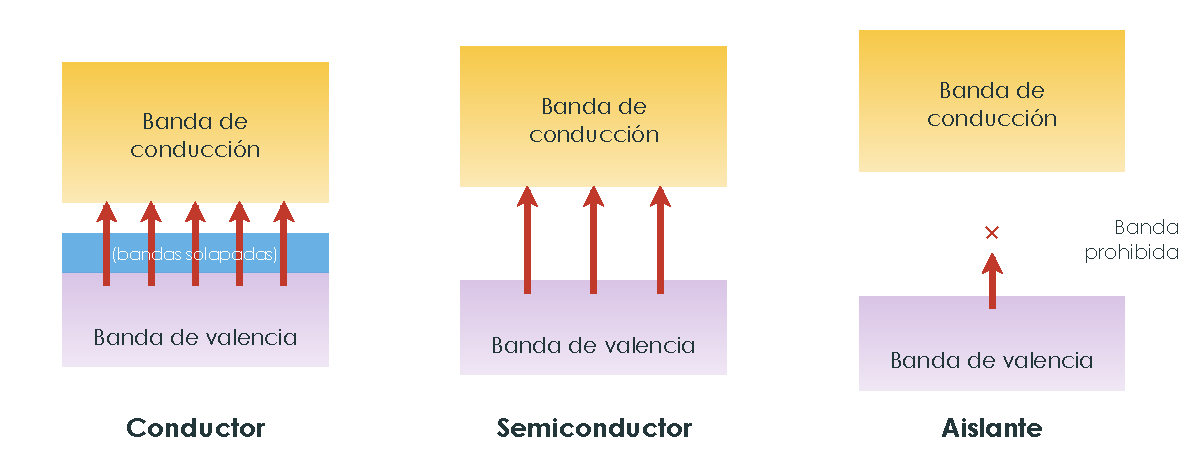
\includegraphics[width=0.75\linewidth]{FigurasSVG/UD3_Enlace_Quimico/pdf/UD3_59_teoria_bandas.pdf}
            \caption{Teoría de bandas}
            \label{fig:teoriadebandas}
        \end{figure}
        \begin{enumerate}[label=\numberballred]
            \item \negrita{Conductores}.
            Son aquellos en los que la banda de valencia y la banda de conducción presentan una diferencia energética muy pequeña o bien están solapando.
            \item \negrita{Semiconductores}.
            Son aquellos en los que la diferencia de la banda de valencia y la banda de conducción no es muy grande.
            \item \negrita{Aislantes}.
            Son aquellos en los que la diferencia de la banda de valencia y la banda de conducción es muy grande.
        \end{enumerate}
\end{enumerate}

\subsection{Propiedades del enlace metálico}\label{subsec:propiedades-del-enlace-metalico}
Las principales propiedades de los metales son:

\begin{enumerate}[label=\numberballmDarkTeal]
        \item Los compuestos metálicos presentan un \textbf{brillo metálico}.
        \item Suelen ser \textbf{sólidos} a excepción del mercurio \ch{Hg}.
        \item Presentan una \textbf{elevada densidad}.
        \item Son \textbf{dúctiles} es decir se deforman en hilos y también son \textbf{maleables} es decir capacidad para deformarse en láminas.
        \item Son buenos \textbf{conductores de la electricidad y el calor}.
        \item Son \textbf{insolubles}.
\end{enumerate}

% \begin{enumerate}[label=\numberballred]
%     \item \negrita{Brillo}. Los compuestos metálicos tienen brillo.
%     \item \negrita{Estado de agregación}. Son sólidos con elevados puntos de ebullición y de fusión.
%     \item \negrita{Densidad}. Presentan una densidad elevada.
%     \item \negrita{Propiedades mecánicas}. Son dúctiles (al deformarse se forman hilos) y maleables (capacidad de deformarse en láminas).
%     \item \negrita{Conductividad eléctrica y térmica}. Son buenos conductores de la electricidad y el calor.
%     \item \negrita{Solubilidad}. Son insolubles en disolventes moléculas.
% \end{enumerate}


%
    \newpage

    %! Author = Profesor
%! Date = 05/06/2024


\section{Ejercicios}\label{sec:ejercicios-UD3}

\subsection{Ejercicios Generales}\label{subsec:ejercicios-generales-UD3}

\begin{exercise}
    Representa las estructuras de Lewis de los compuestos
    \ch{HClO}, \ch{HClO2}, \ch{HClO3} y \ch{HClO4} (ten presente que el átomo
    de H está unido a un átomo de O).
    \begin{solu}
%        \begin{figure}[H]
%            \centering
%            \includegraphics[scale=.5]{images/imagesUD3EnlaceQuimico/UD3_Problemas/cuestiongeneral01}\label{fig:cuestiongeneral01}
%        \end{figure}
        En los cuatro oxoácidos el H está unido a un O (no directamente al Cl), y el Cl es el átomo central unido al resto de átomos de O.

        \textbf{\ch{HClO}}: \(\ch{H-O-Cl}\). El O tiene dos pares solitarios y el Cl tiene tres pares solitarios. Todos los átomos cumplen el octeto.

        \textbf{\ch{HClO2}}: \(\ch{H-O-Cl=O}\). El Cl forma un enlace sencillo con el O del \ch{OH} y un enlace doble con el otro O; le queda un par solitario al Cl. El O del \ch{OH} tiene dos pares solitarios y el O doblemente enlazado tiene dos pares solitarios.

        \textbf{\ch{HClO3}}: \(\ch{H-O-Cl(=O)2}\). El Cl forma un enlace sencillo con el O del \ch{OH} y dos enlaces dobles con los otros dos átomos de O; el Cl no tiene pares solitarios (expande su octeto).

        \textbf{\ch{HClO4}}: \(\ch{H-O-Cl(=O)3}\). El Cl forma un enlace sencillo con el O del \ch{OH} y tres enlaces dobles con los otros tres átomos de O; el Cl no tiene pares solitarios (expande su octeto al máximo).

        En los cuatro casos el Cl expande su capa de valencia por encima de ocho electrones (salvo en el \ch{HClO}), lo cual es posible porque el Cl dispone de orbitales \(d\) de valencia accesibles.
    \end{solu}
\end{exercise}

\begin{exercise}
    Representa las estructuras de Lewis de los iones \ch{ClO-},
    \ch{ClO2-}, \ch{ClO3-}, \ch{ClO4-}(ten presentes las estructuras de los
    oxoácidos que hiciste en el ejercicio anterior).
    \begin{solu}

%        \begin{figure}[H]
%            \centering
%            \includegraphics[scale=.5]{images/imagesUD3EnlaceQuimico/UD3_Problemas/cuestiongeneral02}
%        \end{figure}

        Estos iones se obtienen quitando el H de los oxoácidos del ejercicio anterior; el par de electrones del enlace \ch{O-H} queda íntegramente sobre el O, que adquiere la carga negativa.

        \textbf{\ch{ClO-}}: \([\ch{Cl-O}]^-\). El O tiene tres pares solitarios y carga \(-1\); el Cl tiene tres pares solitarios.

        \textbf{\ch{ClO2-}}: \([\ch{O-Cl=O}]^-\). Existen dos estructuras resonantes equivalentes en las que el enlace doble y la carga negativa se intercambian entre los dos átomos de O; en la estructura real la carga \(-1\) está deslocalizada por igual entre ambos O.

        \textbf{\ch{ClO3-}}: \([\ch{O-Cl(=O)2}]^-\). Hay tres estructuras resonantes; la carga negativa se reparte por igual entre los tres átomos de O.

        \textbf{\ch{ClO4-}}: \([\ch{Cl(=O)4}]^-\). Estructura tetraédrica con resonancia entre los cuatro átomos de O; la carga \(-1\) se distribuye equitativamente entre los cuatro O, lo que explica la gran estabilidad del ion perclorato.
    \end{solu}
\end{exercise}

\begin{exercise}
    Determina la entalpía de sublimación del cinc a partir de
    los siguientes datos, dados según el convenio de signos
    general de energías:
    \begin{figure}[H]
        \centering
        % [FIGURA ORIGINAL] \includegraphics[scale=.5]{images/imagesUD3EnlaceQuimico/UD3_Problemas/energiasejercicio12.png}
        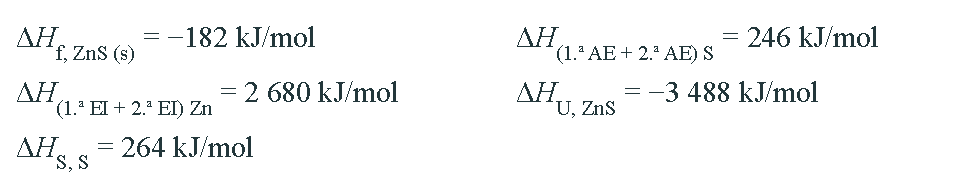
\includegraphics[width=0.7\linewidth]{FigurasSVG/UD3_Enlace_Quimico/pdf/UD3_E01_datos_ZnS.pdf}
    \end{figure}
    \begin{solu}

%        \begin{figure}[H]
%            \centering
%            \includegraphics[scale=.5]{images/imagesUD3EnlaceQuimico/UD3_Problemas/ejerciciogeneral03.png}
%        \end{figure}
%
        Los datos, según el convenio de signos general de energías, son:
        \(\entalpia{f, \ch{ZnS(s)}} = \energia[kj]{-182}\), \(\entalpia{S, S} = \energia[kj]{264}\), \(\entalpia{(1.ª EI + 2.ª EI), Zn} = \energia[kj]{2680}\), \(\entalpia{(1.ª AE + 2.ª AE), S} = \energia[kj]{246}\), \(U_{r, \ch{ZnS}} = \energia[kj]{-3488}\).

        El ciclo de Born-Haber para la formación de \ch{ZnS(s)} a partir de \ch{Zn(s)} y \ch{S(s)} es:
        \[
            \entalpia{f} = \entalpia{sub, Zn} + \entalpia{S, S} + \entalpia{(1.ª EI + 2.ª EI), Zn} + \entalpia{(1.ª AE + 2.ª AE), S} + U_r
        \]

        Despejando la entalpía de sublimación del cinc:
        \[
            \entalpia{sub, Zn} = \entalpia{f} - \entalpia{S, S} - \entalpia{(1.ª EI + 2.ª EI), Zn} - \entalpia{(1.ª AE + 2.ª AE), S} - U_r
        \]
        \[
            \entalpia{sub, Zn} = -182 - 264 - 2680 - 246 - (-3488) = \energia[kj]{116}
        \]

        La entalpía de sublimación del cinc es, por tanto, de \(\energia[kj]{116}\).
    \end{solu}
\end{exercise}


\begin{exercise}
    Asigna los valores de la energía de red correspondientes
    a los siguientes compuestos: \ch{AlCl3}, \ch{KCl}, \ch{CaCl2}, \ch{SrO},
    \ch{CsCl} y \ch{MgO}. Justifica tu respuesta.
    5 376 kJ/mol; 3 796 kJ/mol; 3 217 kJ/mol; 2 268 kJ/mol;
    701 kJ/mol; 657 kJ/mol.

    \begin{solu}

%        \begin{figure}[H]
%            \centering
%            \includegraphics[scale=.5]{images/imagesUD3EnlaceQuimico/UD3_Problemas/ejerciciogeneral04a.png}
%        \end{figure}

        La energía reticular (energía de red) es tanto mayor cuanto mayor es el producto de las cargas de los iones y cuanto menor es la distancia entre ellos (suma de sus radios iónicos), de acuerdo con la ley de Coulomb.

        \begin{itemize}
            \item \ch{AlCl3}: aunque el \ch{Al^{3+}} es pequeño, su carga (\(+3\)) es la más alta de todo el grupo, lo que domina el producto de cargas y le confiere la mayor energía reticular: \(\energia[kjmol]{5376}\).
            \item \ch{MgO} y \ch{SrO}: ambos con producto de cargas \(2\times2=4\), superior al de los cloruros univalentes. Como \ch{Mg^{2+}} es más pequeño que \ch{Sr^{2+}}, \ch{MgO} tiene mayor energía reticular: \(\energia[kjmol]{3796}\), frente a \(\energia[kjmol]{3217}\) del \ch{SrO}.
            \item \ch{CaCl2}: producto de cargas \(2\times1=2\), menor que en los óxidos anteriores: \(\energia[kjmol]{2268}\).
            \item \ch{KCl} y \ch{CsCl}: ambos con producto de cargas \(1\times1=1\), los menores del grupo. Como \ch{K+} es más pequeño que \ch{Cs+}, \ch{KCl} tiene mayor energía reticular: \(\energia[kjmol]{701}\), frente a \(\energia[kjmol]{657}\) del \ch{CsCl}.
        \end{itemize}
    \end{solu}
\end{exercise}


\begin{exercise}
    Ordena los compuestos \ch{AlCl3}, \ch{KCl}, \ch{CaCl2}, \ch{SrO}, \ch{CsCl} y \ch{MgO} según su solubilidad en agua.
    \begin{solu}
        La solubilidad depende de la energía de red. Serán más solubles
        los compuestos de menor energía de red, ya que es más probable
        que la energía de solvatación, debida a las interacciones de
        las moléculas del disolvente con los iones de la red, la compense:

        CsCl \textgreater KCl \textgreater \ch{CaCl2} \textgreater SrO \textgreater MgO \textgreater \ch{AlCl3}
    \end{solu}
\end{exercise}


\begin{exercise}
    Según la TRPECV, indica la geometría y la polaridad de
    estas moléculas (precisa la dirección y el sentido del momento
    dipolar de los enlaces y de las moléculas): \ch{PF3},
    \ch{H2S}, \ch{NH2OH}, \ch{CCl4}, \ch{CClH3}, \ch{BH3}, \ch{PF5}, \ch{OF2} y \ch{BeF2}.

    \begin{solu}

        Primero se hace la representación de Lewis de las moléculas
        y se determina la geometría de la molécula analizando los
        pares de electrones enlazantes y no enlazantes que rodean al
        átomo central. Después se analiza la polaridad de los enlaces
        que forma el átomo central con los otros átomos. Finalmente,
        se determina la polaridad de la molécula, teniendo en cuenta
        que \(\vec{\mu}_{\text{molécula}} = \sum \vec{\mu}_{\text{enlace}} \)

%        \begin{figure}[H]
%            \centering
%            \includegraphics[scale=.5]{images/imagesUD3EnlaceQuimico/UD3_Problemas/ejerciciogeneral06a.png}
%        \end{figure}
%
%        \begin{figure}[H]
%            \centering
%            \includegraphics[scale=.5]{images/imagesUD3EnlaceQuimico/UD3_Problemas/ejerciciogeneral06c.png}
%        \end{figure}
%
%        \begin{figure}[H]
%            \centering
%            \includegraphics[scale=.5]{images/imagesUD3EnlaceQuimico/UD3_Problemas/ejerciciogeneral06c.png}
%        \end{figure}
%
%        \begin{figure}[H]
%            \centering
%            \includegraphics[scale=.5]{images/imagesUD3EnlaceQuimico/UD3_Problemas/ejerciciogeneral06d.png}
%        \end{figure}
%        \begin{figure}[H]
%            \centering
%            \includegraphics[scale=.5]{images/imagesUD3EnlaceQuimico/UD3_Problemas/ejerciciogeneral06e.png}
%        \end{figure}

        % Los momentos dipolares de enlace se dibujan como flechas dirigidas hacia el átomo más electronegativo.
        \begin{center}
            % --- tabla antigua ---
            % \begin{tblr}{hlines, vlines, rows={abovesep=6pt, belowsep=6pt}, colspec={Q[l,m,wd=3.6cm] Q[c,m,wd=4.6cm] Q[c,m,wd=4.6cm]}, row{1}={bg=mybluecolour!15, font=\bfseries}, column{1}={font=\bfseries}}
                                                 % & \ch{PF3} & \ch{H2S} \\
                % Representación de Lewis          & \chemfig{\charge{90=\|,180=\|,270=\|}{F}-\charge{90=\:}{P}(-[6]\charge{0=\|,180=\|,270=\|}{F})-\charge{0=\|,90=\|,270=\|}{F}}
                                                 % & \chemfig{H-\charge{90=\:,270=\:}{S}-H} \\
                % Pares enlazantes                 & 3 & 2 \\
                % Pares no enlazantes              & 1 & 2 \\
                % Geometría del átomo central      & Tetraédrica & Tetraédrica \\
                % Geometría de la molécula         & Piramidal & Angular \\
                % \(EN\) de los elementos          & P (\num{2.1}); F (\num{4.0}) & S (\num{2.5}); H (\num{2.1}) \\
                % {Polaridad de la molécula \\ {\footnotesize\(\left(\vec{\mu}_{\text{molécula}} = \sum \vec{\mu}_{\text{enlace}}\right)\)}}
                                                 % & {\chemfig{\charge{90=\:}{P}(-[:-150,,,,-stealth]F)(-[:-30,,,,-stealth]F)-[:15,,,,-stealth]F} \\ \rule{0pt}{3.5ex}\(\vec{\mu}_{\text{molécula}} \neq 0\)}
                                                 % & {\chemfig{H-[:30,,,,-stealth]\charge{45=\:,135=\:}{S}-[:-30,,,,stealth-]H} \\ \rule{0pt}{3.5ex}\(\vec{\mu}_{\text{molécula}} \neq 0\)} \\
            % \end{tblr}
            % --- tabla nueva ---
            \begin{tabular}{@{}L{3.6cm} C{4.6cm} C{4.6cm}@{}}
                \toprule
                 & \textbf{\ch{PF3}} & \textbf{\ch{H2S}} \\
                \midrule
                \textbf{Representación de Lewis} & \chemfig{\charge{90=\|,180=\|,270=\|}{F}-\charge{90=\:}{P}(-[6]\charge{0=\|,180=\|,270=\|}{F})-\charge{0=\|,90=\|,270=\|}{F}} & \chemfig{H-\charge{90=\:,270=\:}{S}-H} \\[3pt]
                \textbf{Pares enlazantes} & 3 & 2 \\[3pt]
                \textbf{Pares no enlazantes} & 1 & 2 \\[3pt]
                \textbf{Geometría del átomo central} & Tetraédrica & Tetraédrica \\[3pt]
                \textbf{Geometría de la molécula} & Piramidal & Angular \\[3pt]
                \textbf{\(EN\) de los elementos} & P (\num{2.1}); F (\num{4.0}) & S (\num{2.5}); H (\num{2.1}) \\[3pt]
                \textbf{Polaridad de la molécula \newline {\footnotesize\(\left(\vec{\mu}_{\text{molécula}} = \sum \vec{\mu}_{\text{enlace}}\right)\)}} & \chemfig{\charge{90=\:}{P}(-[:-150,,,,-stealth]F)(-[:-30,,,,-stealth]F)-[:15,,,,-stealth]F} \newline \rule{0pt}{3.5ex}\(\vec{\mu}_{\text{molécula}} \neq 0\) & \chemfig{H-[:30,,,,-stealth]\charge{45=\:,135=\:}{S}-[:-30,,,,stealth-]H} \newline \rule{0pt}{3.5ex}\(\vec{\mu}_{\text{molécula}} \neq 0\) \\
                \bottomrule
            \end{tabular}
        \end{center}

        \begin{center}
            % --- tabla antigua ---
            % \begin{tblr}{hlines, vlines, rows={abovesep=6pt, belowsep=6pt}, colspec={Q[l,m,wd=3.6cm] Q[c,m,wd=4.6cm] Q[c,m,wd=4.6cm]}, row{1}={bg=mybluecolour!15, font=\bfseries}, column{1}={font=\bfseries}}
                                                 % & \ch{NH2OH} & \ch{CCl4} \\
                % Representación de Lewis          & \chemfig{H-\charge{90=\:}{N}(-[6]H)-\charge{90=\:,270=\:}{O}-H}
                                                 % & \chemfig{C(-[2]\charge{0=\|,90=\|,180=\|}{Cl})(-[4]\charge{90=\|,180=\|,270=\|}{Cl})(-[6]\charge{0=\|,180=\|,270=\|}{Cl})-\charge{0=\|,90=\|,270=\|}{Cl}} \\
                % Pares enlazantes                 & 3 & 4 \\
                % Pares no enlazantes              & 1 & 0 \\
                % Geometría del átomo central      & Tetraédrica & Tetraédrica \\
                % Geometría de la molécula         & Piramidal & Tetraédrica \\
                % \(EN\) de los elementos          & N (\num{3.0}); O (\num{3.5}); H (\num{2.1}) & C (\num{2.5}); Cl (\num{3.0}) \\
                % {Polaridad de la molécula \\ {\footnotesize\(\left(\vec{\mu}_{\text{molécula}} = \sum \vec{\mu}_{\text{enlace}}\right)\)}}
                                                 % & {\chemfig{\charge{90=\:}{N}(-[:-150,,,,stealth-]H)(-[:-30,,,,-stealth]OH)-[:15,,,,stealth-]H} \\ \rule{0pt}{3.5ex}\(\vec{\mu}_{\text{molécula}} \neq 0\)}
                                                 % & {\chemfig{C(-[2,,,,-stealth]Cl)(-[0,,,,-stealth]Cl)(-[:-130,,,,-stealth]Cl)-[:-50,,,,-stealth]Cl} \\ \rule{0pt}{3.5ex}\(\vec{\mu}_{\text{molécula}} = 0\)} \\
            % \end{tblr}
            % --- tabla nueva ---
            \begin{tabular}{@{}L{3.6cm} C{4.6cm} C{4.6cm}@{}}
                \toprule
                 & \textbf{\ch{NH2OH}} & \textbf{\ch{CCl4}} \\
                \midrule
                \textbf{Representación de Lewis} & \chemfig{H-\charge{90=\:}{N}(-[6]H)-\charge{90=\:,270=\:}{O}-H} & \chemfig{C(-[2]\charge{0=\|,90=\|,180=\|}{Cl})(-[4]\charge{90=\|,180=\|,270=\|}{Cl})(-[6]\charge{0=\|,180=\|,270=\|}{Cl})-\charge{0=\|,90=\|,270=\|}{Cl}} \\[3pt]
                \textbf{Pares enlazantes} & 3 & 4 \\[3pt]
                \textbf{Pares no enlazantes} & 1 & 0 \\[3pt]
                \textbf{Geometría del átomo central} & Tetraédrica & Tetraédrica \\[3pt]
                \textbf{Geometría de la molécula} & Piramidal & Tetraédrica \\[3pt]
                \textbf{\(EN\) de los elementos} & N (\num{3.0}); O (\num{3.5}); H (\num{2.1}) & C (\num{2.5}); Cl (\num{3.0}) \\[3pt]
                \textbf{Polaridad de la molécula \newline {\footnotesize\(\left(\vec{\mu}_{\text{molécula}} = \sum \vec{\mu}_{\text{enlace}}\right)\)}} & \chemfig{\charge{90=\:}{N}(-[:-150,,,,stealth-]H)(-[:-30,,,,-stealth]OH)-[:15,,,,stealth-]H} \newline \rule{0pt}{3.5ex}\(\vec{\mu}_{\text{molécula}} \neq 0\) & \chemfig{C(-[2,,,,-stealth]Cl)(-[0,,,,-stealth]Cl)(-[:-130,,,,-stealth]Cl)-[:-50,,,,-stealth]Cl} \newline \rule{0pt}{3.5ex}\(\vec{\mu}_{\text{molécula}} = 0\) \\
                \bottomrule
            \end{tabular}
        \end{center}

        \begin{center}
            % --- tabla antigua ---
            % \begin{tblr}{hlines, vlines, rows={abovesep=6pt, belowsep=6pt}, colspec={Q[l,m,wd=3.6cm] Q[c,m,wd=4.6cm] Q[c,m,wd=4.6cm]}, row{1}={bg=mybluecolour!15, font=\bfseries}, column{1}={font=\bfseries}}
                                                 % & \ch{CClH3} & \ch{BH3} \\
                % Representación de Lewis          & \chemfig{C(-[2]H)(-[4]H)(-[0]H)-[6]\charge{0=\|,180=\|,270=\|}{Cl}}
                                                 % & \chemfig{H-B(-[6]H)-H} \\
                % Pares enlazantes                 & 4 & 3 \\
                % Pares no enlazantes              & 0 & 0 \\
                % Geometría del átomo central      & Tetraédrica & Triangular \\
                % Geometría de la molécula         & Tetraédrica & Triangular \\
                % \(EN\) de los elementos          & C (\num{2.5}); H (\num{2.1}); Cl (\num{3.0}) & B (\num{2.0}); H (\num{2.1}) \\
                % {Polaridad de la molécula \\ {\footnotesize\(\left(\vec{\mu}_{\text{molécula}} = \sum \vec{\mu}_{\text{enlace}}\right)\)}}
                                                 % & {\chemfig{C(-[2,,,,-stealth]Cl)(-[0,,,,stealth-]H)(-[:-130,,,,stealth-]H)-[:-50,,,,stealth-]H} \\ \rule{0pt}{3.5ex}\(\vec{\mu}_{\text{molécula}} \neq 0\)}
                                                 % & {\chemfig{B(-[:150,,,,-stealth]H)(-[:30,,,,-stealth]H)-[6,,,,-stealth]H} \\ \rule{0pt}{3.5ex}\(\vec{\mu}_{\text{molécula}} = 0\)} \\
            % \end{tblr}
            % --- tabla nueva ---
            \begin{tabular}{@{}L{3.6cm} C{4.6cm} C{4.6cm}@{}}
                \toprule
                 & \textbf{\ch{CClH3}} & \textbf{\ch{BH3}} \\
                \midrule
                \textbf{Representación de Lewis} & \chemfig{C(-[2]H)(-[4]H)(-[0]H)-[6]\charge{0=\|,180=\|,270=\|}{Cl}} & \chemfig{H-B(-[6]H)-H} \\[3pt]
                \textbf{Pares enlazantes} & 4 & 3 \\[3pt]
                \textbf{Pares no enlazantes} & 0 & 0 \\[3pt]
                \textbf{Geometría del átomo central} & Tetraédrica & Triangular \\[3pt]
                \textbf{Geometría de la molécula} & Tetraédrica & Triangular \\[3pt]
                \textbf{\(EN\) de los elementos} & C (\num{2.5}); H (\num{2.1}); Cl (\num{3.0}) & B (\num{2.0}); H (\num{2.1}) \\[3pt]
                \textbf{Polaridad de la molécula \newline {\footnotesize\(\left(\vec{\mu}_{\text{molécula}} = \sum \vec{\mu}_{\text{enlace}}\right)\)}} & \chemfig{C(-[2,,,,-stealth]Cl)(-[0,,,,stealth-]H)(-[:-130,,,,stealth-]H)-[:-50,,,,stealth-]H} \newline \rule{0pt}{3.5ex}\(\vec{\mu}_{\text{molécula}} \neq 0\) & \chemfig{B(-[:150,,,,-stealth]H)(-[:30,,,,-stealth]H)-[6,,,,-stealth]H} \newline \rule{0pt}{3.5ex}\(\vec{\mu}_{\text{molécula}} = 0\) \\
                \bottomrule
            \end{tabular}
        \end{center}

        \begin{center}
            % --- tabla antigua ---
            % \begin{tblr}{hlines, vlines, rows={abovesep=6pt, belowsep=6pt}, colspec={Q[l,m,wd=3.6cm] Q[c,m,wd=4.6cm] Q[c,m,wd=4.6cm]}, row{1}={bg=mybluecolour!15, font=\bfseries}, column{1}={font=\bfseries}}
                                                 % & \ch{PF5} & \ch{OF2} \\
                % Representación de Lewis          & \chemfig{P(-[2]\charge{0=\|,90=\|,180=\|}{F})(-[:160]\charge{90=\|,180=\|,270=\|}{F})(-[:20]\charge{0=\|,90=\|,270=\|}{F})(-[:-120]\charge{0=\|,180=\|,270=\|}{F})-[:-60]\charge{0=\|,180=\|,270=\|}{F}}
                                                 % & \chemfig{\charge{90=\|,180=\|,270=\|}{F}-\charge{90=\:,270=\:}{O}-\charge{0=\|,90=\|,270=\|}{F}} \\
                % Pares enlazantes                 & 5 & 2 \\
                % Pares no enlazantes              & 0 & 2 \\
                % Geometría del átomo central      & Bipirámide triangular & Tetraédrica \\
                % Geometría de la molécula         & Bipirámide triangular & Angular \\
                % \(EN\) de los elementos          & P (\num{2.1}); F (\num{4.0}) & O (\num{3.5}); F (\num{4.0}) \\
                % {Polaridad de la molécula \\ {\footnotesize\(\left(\vec{\mu}_{\text{molécula}} = \sum \vec{\mu}_{\text{enlace}}\right)\)}}
                                                 % & {\chemfig{P(-[2,,,,-stealth]F)(-[6,,,,-stealth]F)(-[4,,,,-stealth]F)(-[:30,,,,-stealth]F)-[:-30,,,,-stealth]F} \\ \rule{0pt}{3.5ex}\(\vec{\mu}_{\text{molécula}} = 0\)}
                                                 % & {\chemfig{\charge{60=\:,120=\:}{O}(-[:-135,,,,-stealth]F)-[:-45,,,,-stealth]F} \\ \rule{0pt}{3.5ex}\(\vec{\mu}_{\text{molécula}} \neq 0\)} \\
            % \end{tblr}
            % --- tabla nueva ---
            \begin{tabular}{@{}L{3.6cm} C{4.6cm} C{4.6cm}@{}}
                \toprule
                 & \textbf{\ch{PF5}} & \textbf{\ch{OF2}} \\
                \midrule
                \textbf{Representación de Lewis} & \chemfig{P(-[2]\charge{0=\|,90=\|,180=\|}{F})(-[:160]\charge{90=\|,180=\|,270=\|}{F})(-[:20]\charge{0=\|,90=\|,270=\|}{F})(-[:-120]\charge{0=\|,180=\|,270=\|}{F})-[:-60]\charge{0=\|,180=\|,270=\|}{F}} & \chemfig{\charge{90=\|,180=\|,270=\|}{F}-\charge{90=\:,270=\:}{O}-\charge{0=\|,90=\|,270=\|}{F}} \\[3pt]
                \textbf{Pares enlazantes} & 5 & 2 \\[3pt]
                \textbf{Pares no enlazantes} & 0 & 2 \\[3pt]
                \textbf{Geometría del átomo central} & Bipirámide triangular & Tetraédrica \\[3pt]
                \textbf{Geometría de la molécula} & Bipirámide triangular & Angular \\[3pt]
                \textbf{\(EN\) de los elementos} & P (\num{2.1}); F (\num{4.0}) & O (\num{3.5}); F (\num{4.0}) \\[3pt]
                \textbf{Polaridad de la molécula \newline {\footnotesize\(\left(\vec{\mu}_{\text{molécula}} = \sum \vec{\mu}_{\text{enlace}}\right)\)}} & \chemfig{P(-[2,,,,-stealth]F)(-[6,,,,-stealth]F)(-[4,,,,-stealth]F)(-[:30,,,,-stealth]F)-[:-30,,,,-stealth]F} \newline \rule{0pt}{3.5ex}\(\vec{\mu}_{\text{molécula}} = 0\) & \chemfig{\charge{60=\:,120=\:}{O}(-[:-135,,,,-stealth]F)-[:-45,,,,-stealth]F} \newline \rule{0pt}{3.5ex}\(\vec{\mu}_{\text{molécula}} \neq 0\) \\
                \bottomrule
            \end{tabular}
        \end{center}

        \begin{center}
            % --- tabla antigua ---
            % \begin{tblr}{hlines, vlines, rows={abovesep=6pt, belowsep=6pt}, colspec={Q[l,m,wd=6cm] Q[c,m,wd=4.6cm]}, row{1}={bg=mybluecolour!15, font=\bfseries}, column{1}={font=\bfseries}}
                                                 % & \ch{BeF2} \\
                % Representación de Lewis          & \chemfig{\charge{90=\:,180=\:,270=\:}{F}-Be-\charge{0=\:,90=\:,270=\:}{F}} \\
                % Pares enlazantes                 & 2 \\
                % Pares no enlazantes              & 0 \\
                % Geometría del átomo central      & Lineal \\
                % Geometría de la molécula         & Lineal \\
                % \(EN\) de los elementos          & Be (\num{1.5}); F (\num{4.0}) \\
                % {Polaridad de la molécula \\ {\footnotesize\(\left(\vec{\mu}_{\text{molécula}} = \sum \vec{\mu}_{\text{enlace}}\right)\)}}
                                                 % & {\chemfig{F-[,,,,stealth-]Be-[,,,,-stealth]F} \\ \rule{0pt}{3.5ex}\(\vec{\mu}_{\text{molécula}} = 0\)} \\
            % \end{tblr}
            % --- tabla nueva ---
            \begin{tabular}{@{}L{6cm} C{4.6cm}@{}}
                \toprule
                 & \textbf{\ch{BeF2}} \\
                \midrule
                \textbf{Representación de Lewis} & \chemfig{\charge{90=\:,180=\:,270=\:}{F}-Be-\charge{0=\:,90=\:,270=\:}{F}} \\[3pt]
                \textbf{Pares enlazantes} & 2 \\[3pt]
                \textbf{Pares no enlazantes} & 0 \\[3pt]
                \textbf{Geometría del átomo central} & Lineal \\[3pt]
                \textbf{Geometría de la molécula} & Lineal \\[3pt]
                \textbf{\(EN\) de los elementos} & Be (\num{1.5}); F (\num{4.0}) \\[3pt]
                \textbf{Polaridad de la molécula \newline {\footnotesize\(\left(\vec{\mu}_{\text{molécula}} = \sum \vec{\mu}_{\text{enlace}}\right)\)}} & \chemfig{F-[,,,,stealth-]Be-[,,,,-stealth]F} \newline \rule{0pt}{3.5ex}\(\vec{\mu}_{\text{molécula}} = 0\) \\
                \bottomrule
            \end{tabular}
        \end{center}

    \end{solu}
\end{exercise}

\begin{exercise}
    Haz un estudio de la estructura de la molécula
    \chemfig{CH_2Cl-C~N}. Indica qué orbitales forman cada enlace y
    cómo son los ángulos de enlace.
    \begin{solu}
%        \begin{figure}[H]
%            \centering
%            \includegraphics[scale=.6]{images/imagesUD3EnlaceQuimico/UD3_Problemas/ejerciciogeneral07.png}
%        \end{figure}
        La molécula \(\ch{CH2Cl-C+N}\) (cloroacetonitrilo) tiene dos átomos de carbono con hibridaciones distintas:

        \begin{itemize}
            \item El carbono metilénico (\(\ch{CH2Cl}\)) presenta hibridación \(sp^3\): forma cuatro enlaces \(\sigma\) sencillos (dos con H, mediante solapamiento \(sp^3\)-\(s\); uno con Cl, mediante solapamiento \(sp^3\)-\(p\); y uno con el otro C, mediante solapamiento \(sp^3\)-\(sp\)). Los ángulos de enlace en torno a este carbono son de, aproximadamente, \(109{,}5°\) (geometría tetraédrica).
            \item El carbono nitrílico presenta hibridación \(sp\): forma un enlace \(\sigma\) sencillo con el carbono anterior (solapamiento \(sp\)-\(sp^3\)) y un enlace triple con el N, constituido por un enlace \(\sigma\) (solapamiento \(sp\)-\(sp\)) y dos enlaces \(\pi\) (solapamiento de los dos orbitales \(p\) no hibridados de cada átomo, perpendiculares entre sí). El ángulo \(\ch{C-C+N}\) es de \(180°\) (geometría lineal en torno a este carbono).
            \item El átomo de N, también con hibridación \(sp\), completa el enlace triple con el carbono y aloja un par de electrones solitario en el orbital \(sp\) restante, dirigido en línea recta con el resto de la molécula.
        \end{itemize}
    \end{solu}
\end{exercise}


\begin{exercise}
    Para las moléculas \chemfig{H-CHO}, \ch{CH3OH} y \ch{CH3OCH3}:
    a) Deduce a partir de sus estructuras de Lewis cuál tiene
    menor longitud de enlace CO.
    b) Justifica si alguna de ellas presenta enlace de H.
    \begin{solu}
%        \begin{figure}[H]
%            \centering
%            \includegraphics[scale=.6]{images/imagesUD3EnlaceQuimico/UD3_Problemas/ejerciciogeneral08.png}
%        \end{figure}
        a) El \ch{H-CHO} (metanal) tiene un enlace \ch{C=O} doble, con longitud de enlace corta (mayor orden de enlace, dos pares de electrones compartidos), mientras que el \ch{CH3OH} y el \ch{CH3OCH3} tienen un enlace \ch{C-O} sencillo, más largo. Por tanto, el \ch{H-CHO} presenta \textbf{menor longitud de enlace \ch{C-O}} que los otros dos compuestos.

        b) El enlace de hidrógeno se establece entre un átomo de H unido a un átomo muy electronegativo (F, O, N) y un par solitario de otro átomo electronegativo de una molécula vecina; requiere, por tanto, un grupo \ch{O-H} (o \ch{N-H}, \ch{F-H}). Solo el \ch{CH3OH} posee un grupo \ch{-OH}, por lo que es la única de las tres moléculas capaz de establecer enlaces de H entre sus propias moléculas (actuando a la vez como dador y aceptor). El \ch{H-CHO} y el \ch{CH3OCH3} tienen átomo de O, por lo que pueden actuar como \emph{aceptores} de enlace de H frente a otras moléculas que sí tengan \ch{-OH} (como el agua), pero no pueden formar enlaces de H entre sus propias moléculas, al carecer de H unido a un átomo electronegativo.
    \end{solu}
\end{exercise}

\begin{exercise}
    Dadas las moléculas \ch{H2O}, \ch{HF}, \ch{H2}, \ch{CH4} y \ch{NH3}, contesta
    justificadamente a cada una de las siguientes cuestiones:
    a) ¿Cuál o cuáles son polares?
    b) ¿Cuál presenta el enlace con mayor contribución iónica?
    c) ¿Cuál presenta el enlace con mayor contribución covalente?
    d) ¿Cuál o cuáles pueden presentar enlace de hidrógeno?
    \begin{solu}
%        \begin{figure}[H]
%            \centering
%            \includegraphics[scale=.6]{images/imagesUD3EnlaceQuimico/UD3_Problemas/ejerciciogeneral08.png}
%        \end{figure}
        a) \ch{H2O}: molécula angular con enlaces polares → molécula polar;
        \ch{HF}: enlace polar, molécula polar; \ch{H2}: enlace apolar, molécula
        apolar; \ch{CH4}: enlaces poco polares, molécula tetraédrica
        perfectamente simétrica → molécula apolar; NH3: enlaces
        polares, molécula piramidal → molécula polar.
        b) El enlace con mayor contribución iónica es el enlace más
        polar: enlace \ch{H-F}.
        c) El enlace con mayor contribución covalente es el enlace
        menos polar: enlace \ch{H-H}.
        d) Pueden presentar enlaces de H las moléculas que contengan
        enlaces \ch{-OH}, \ch{F-H} y \ch{-NH}. En este caso, las moléculas
        de \ch{H2O}, \ch{HF} y \ch{NH3}.
    \end{solu}
\end{exercise}


\begin{exercise}
    Indica, razonadamente, qué tipo de interacción o enlace
    químico se rompe para:
    a) Fundir cloruro de potasio. c) Hervir agua.
    b) Disolver yodo en benceno. d) Sublimar sodio.
    \begin{solu}

%        \begin{figure}[H]
%            \centering
%            \includegraphics[scale=.6]{images/imagesUD3EnlaceQuimico/UD3_Problemas/ejerciciogeneral10a.png}
%            \includegraphics[scale=.6]{images/imagesUD3EnlaceQuimico/UD3_Problemas/ejerciciogeneral10b.png}
%        \end{figure}

        \begin{itemize}
            \item[a)] \textbf{Fundir cloruro de potasio}: se rompe el \textbf{enlace iónico}, es decir, la red cristalina que mantiene unidos los iones \ch{K+} y \ch{Cl-}.
            \item[b)] \textbf{Disolver yodo en benceno}: se rompen las \textbf{fuerzas de dispersión de London} (van der Waals) que mantienen unidas entre sí las moléculas apolares de \ch{I2}.
            \item[c)] \textbf{Hervir agua}: se rompen los \textbf{enlaces de hidrógeno} que mantienen unidas las moléculas de \ch{H2O} en estado líquido.
            \item[d)] \textbf{Sublimar sodio}: se rompe el \textbf{enlace metálico} que mantiene unidos los átomos de Na en la red metálica.
        \end{itemize}
    \end{solu}
\end{exercise}



\begin{exercise}
    A la presión atmosférica, el \ch{H2O} tiene un punto de ebullición
    de 100 °C; el \ch{CH3OH}, de 64,5 °C, y el \ch{C2H5OH}, de
    78 °C. Justifica este hecho sobre la base de los enlaces
    intermoleculares que se dan en esas sustancias.
    \begin{solu}
        Las tres sustancias presentan enlace de H, ya que tienen
        \ch{O-H}. Cada molécula de agua puede formar dos enlaces de
        H, ya que tiene dos grupos OH, mientras que una molécula
        de etanol o de metanol solo puede formar uno; por esta razón,
        el punto de ebullición del agua es mayor. Entre los dos
        alcoholes, el de mayor punto de ebullición es el etanol, ya
        que, tratándose de moléculas de la misma serie homóloga,
        la de mayor masa molar es la que presenta mayor punto de
        ebullición.
    \end{solu}
\end{exercise}


\begin{exercise}
    Calcula la energía de red (energía reticular) del cloruro de magnesio tomando como datos: $\entalpia{sub} =  \energia[kj]{147.7}$, $EI (\text{1º y 2º}) = \energia[kj]{2188}$,  $\entalpia{dis} =  \energia[kj]{244}$, $AE = \energia[kj]{-348}$, $\entalpia{f} =  \energia[kjmol]{-642}$
    \begin{solu}

        El ciclo de Born-Haber para la formación de \ch{MgCl2(s)} a partir de \ch{Mg(s)} y \ch{Cl2(g)} es:
        \[
            \entalpia{f} = \entalpia{sub} + EI(\text{1º y 2º}) + \entalpia{dis} + 2 \, AE + U_r
        \]

        El factor 2 en la afinidad electrónica se debe a que se forman dos iones \ch{Cl-} por cada unidad de \ch{MgCl2}, mientras que la disociación de \ch{Cl2} ya proporciona directamente los dos átomos de Cl necesarios.

        Despejando la energía reticular:
        \[
            U_r = \entalpia{f} - \entalpia{sub} - EI(\text{1º y 2º}) - \entalpia{dis} - 2 \, AE
        \]
        \[
            U_r = -642 - 147{,}7 - 2188 - 244 - 2\cdot(-348) = \energia[kj]{-2525,7}
        \]

        La energía de red del cloruro de magnesio es, por tanto, de \(\energia[kj]{-2525,7}\) (energía liberada al formarse el sólido iónico a partir de los iones gaseosos).
    \end{solu}
\end{exercise}

\begin{exercise}
    Calcula la afinidad electrónica del oxígeno para dar \ch{O\mch[2]} (suma de la primera y segunda AE), a partir del ciclo de Born-Haber del óxido de sodio. Datos: $\entalpia{f, \ch{Na2O (s)}} = \energia[kjmol]{-414,2} -414.2$, $\entalpia{dis,\ch{O2}} = \energia[kjmol]{494}$, $\entalpia{sub, \ch{Na}} = \energia[kjmol]{107,3}$, $EI_{Na} = \energia[kjmol]{495,8}$, $U_r{\ch{Na2O(s)}} = \energia[kjmol]{-2604,4}$
    \begin{solu}

%        \begin{figure}[H]
%            \centering
%            \includegraphics[scale=.5]{images/imagesUD3EnlaceQuimico/UD3_Problemas/ejerciciogeneral13.png}
%            %\caption{}
%            %\label{fig:}
%        \end{figure}

        El ciclo de Born-Haber para la formación de \ch{Na2O(s)} a partir de \ch{2Na(s)} y \(\frac{1}{2}\)\ch{O2(g)} es:
        \[
            \entalpia{f} = 2\,\entalpia{sub, Na} + 2\,EI_{Na} + \tfrac{1}{2}\entalpia{dis, \ch{O2}} + AE_{(1.ª+2.ª), O} + U_r
        \]

        Despejando la suma de la primera y segunda afinidad electrónica del oxígeno:
        \[
            AE_{(1.ª+2.ª), O} = \entalpia{f} - 2\,\entalpia{sub, Na} - 2\,EI_{Na} - \tfrac{1}{2}\entalpia{dis, \ch{O2}} - U_r
        \]
        \[
            AE_{(1.ª+2.ª), O} = -414{,}2 - 2\cdot107{,}3 - 2\cdot495{,}8 - \tfrac{1}{2}\cdot494 - (-2604{,}4) = \energia[kjmol]{737,0}
        \]

        La suma de la primera y segunda afinidad electrónica del oxígeno es de \(\energia[kjmol]{737,0}\), un valor positivo (proceso globalmente endotérmico), ya que la primera AE del O es exotérmica pero la segunda (incorporar un electrón a un ion \ch{O-} ya negativo) es muy endotérmica, y esta última domina la suma.
    \end{solu}
\end{exercise}



\begin{exercise}
    Asigna los puntos de fusión \temperatura[c]{642}, \temperatura[c]{734}, \temperatura[c]{996} aproximados a cada una de estas sustancias, \ch{KBr}, \ch{RbI} y \ch{NaF}.
    Justifícalo según los datos de la tabla.
    \begin{figure}[H]
        \centering
        \begin{tblr}{|c|c|c|c|}
            \hline
            Compuesto            & \ch{KBr} & \ch{RbI} & \ch{NaF } \\
            \hline
            Energía de reticular & 682      & 630      & 923       \\
            \hline
            Punto de fusión & 734 & 642 & 996 \\
            \hline
        \end{tblr}

    \end{figure}
%    \begin{figure}[H]
%        \centering
%        \includegraphics[scale=0.5]{images/imagesUD3EnlaceQuimico/UD3_Problemas/tabla_ejer_fusion.png}
%        %\caption{}
%        \label{fig:tabla_ejer}
%    \end{figure}
    \begin{solu}

        Para fundir un compuesto iónico, hay que romper la red cristalina. Por tanto, el punto de fusión es tanto más alto cuanto mayor sea la energía reticular (energía de red).

    \end{solu}
\end{exercise}


\begin{exercise}
    Explica qué le ocurre a la energía reticular de los compuestos iónicos del tipo \ch{A^{x+}} y \ch{B^{y-}} si:
    \begin{enumerate}[label=\letraminuscula]
        \item Se duplica la carga del anión.
        \item Se reduce a la mitad la carga del catión.
        \item Aumenta el tamaño del anión.
        \item Aumenta el tamaño del catión.
        \item Se incrementa el coeficiente o factor de Born.
        \item Los iones pasan de tener estructura de tipo Ar a tenerla tipo Ne.
        \item Disminuye la constante de Madelung.
    \end{enumerate}
    \begin{solu}

        La energía reticular sigue, de forma aproximada, la expresión de Born-Landé:
        \[
            U_r = -\frac{N_A \, M \, z_+ \, z_- \, e^2}{4\pi\varepsilon_0 \, r_0}\left(1-\frac{1}{n}\right)
        \]
        donde \(z_+\) y \(z_-\) son las cargas de los iones, \(r_0\) la distancia entre sus centros (suma de radios iónicos), \(M\) la constante de Madelung y \(n\) el factor (exponente) de Born.

        \begin{enumerate}[label=\letraminuscula]
            \item Al duplicarse la carga del anión, el producto \(z_+ z_-\) se duplica, por lo que la energía reticular \textbf{se duplica aproximadamente} (en valor absoluto aumenta).
            \item Al reducirse a la mitad la carga del catión, el producto \(z_+ z_-\) se reduce a la mitad, por lo que la energía reticular \textbf{se reduce aproximadamente a la mitad}.
            \item Al aumentar el tamaño del anión, aumenta \(r_0\), por lo que la energía reticular \textbf{disminuye} (en valor absoluto).
            \item Al aumentar el tamaño del catión, aumenta \(r_0\), por lo que la energía reticular \textbf{disminuye} (en valor absoluto), igual que en el caso anterior.
            \item Al incrementarse el factor de Born \(n\), el término \(\left(1-\dfrac{1}{n}\right)\) aumenta (se acerca a 1), por lo que la energía reticular \textbf{aumenta ligeramente} en valor absoluto.
            \item Los iones con estructura tipo Ar tienen un factor de Born mayor (\(n\approx9\)) que los de tipo Ne (\(n\approx7\)). Al pasar de tipo Ar a tipo Ne, \(n\) disminuye, el término \(\left(1-\dfrac{1}{n}\right)\) disminuye y, por tanto, la energía reticular \textbf{disminuye ligeramente} en valor absoluto.
            \item Como \(U_r\) es directamente proporcional a la constante de Madelung \(M\), si esta disminuye, la energía reticular \textbf{disminuye} en valor absoluto.
        \end{enumerate}
    \end{solu}
\end{exercise}

\begin{exercise}
    %!Página 112 Ejercicio 1
    \begin{enumerate}[label=\letraminuscula]
        \item ¿Qué es un enlace químico?
        \item ¿Qué tipos de enlace conoces?
        \item ¿Entre qué elementos de la tabla periódica se produce cada uno de los enlaces?
    \end{enumerate}
    Cita tres sustancias con cada uno de los tres tipos principales de enlace que conoces.
    \begin{solu}

        \begin{enumerate}[label=\letraminuscula]
            \item Un enlace químico es el conjunto de fuerzas que mantiene unidos a los átomos o iones cuando forman moléculas, cristales o redes metálicas.
            \item Los tres tipos principales de enlace son el \textbf{iónico}, el \textbf{covalente} y el \textbf{metálico}.
            \item El enlace \textbf{iónico} se produce entre un elemento metálico (grupos 1-2 y metales de transición, baja electronegatividad) y un elemento no metálico (grupos 16-17, alta electronegatividad), con una diferencia de electronegatividad grande. El enlace \textbf{covalente} se produce entre elementos no metálicos (parte derecha de la tabla), con electronegatividades altas y similares. El enlace \textbf{metálico} se produce entre átomos de elementos metálicos entre sí.
        \end{enumerate}

        Ejemplos: enlace iónico: \ch{NaCl}, \ch{CaO}, \ch{KBr}. Enlace covalente: \ch{H2O}, \ch{CO2}, \ch{HCl}. Enlace metálico: Fe, Cu, Na.
    \end{solu}
\end{exercise}

\begin{exercise}
    %!Página 112 Ejercicio 10 Bruño
    ¿Es cierta la siguiente afirmación: Solo los compuestos pueden tener enlace iónico?
    \begin{solu}

        Sí, es cierta. El enlace iónico se produce por transferencia de electrones entre átomos de electronegatividades muy distintas (un metal, que cede electrones, y un no metal, que los capta), formando un catión y un anión que se atraen electrostáticamente. Como esta transferencia solo tiene sentido entre átomos de \textbf{elementos diferentes}, el enlace iónico siempre da lugar a un \textbf{compuesto} (sustancia formada por al menos dos elementos distintos), y nunca a una sustancia elemental (formada por átomos de un único elemento, con igual electronegatividad, entre los que no puede haber transferencia neta de electrones).
    \end{solu}
\end{exercise}

\begin{exercise}
    %!Página 112 Ejercicio 11
    Escribe los iones que pueden formar los elementos: Li, Cs, Ag, Zn, Cu, Ti, F, O, As, N, I, Se, Te.
    \begin{solu}

        Los metales tienden a perder sus electrones de valencia para adquirir configuración de gas noble (o de capa \(d\) completa), formando cationes; los no metales tienden a ganar electrones hasta completar el octeto, formando aniones:

        \begin{itemize}
            \item Li \(\rightarrow\) \ch{Li+}
            \item Cs \(\rightarrow\) \ch{Cs+}
            \item Ag \(\rightarrow\) \ch{Ag+}
            \item Zn \(\rightarrow\) \ch{Zn^{2+}}
            \item Cu \(\rightarrow\) \ch{Cu+} y \ch{Cu^{2+}} (presenta dos estados de oxidación habituales)
            \item Ti \(\rightarrow\) \ch{Ti^{2+}}, \ch{Ti^{3+}} y \ch{Ti^{4+}} (siendo este último el más estable)
            \item F \(\rightarrow\) \ch{F-}
            \item O \(\rightarrow\) \ch{O^{2-}}
            \item As \(\rightarrow\) \ch{As^{3-}}
            \item N \(\rightarrow\) \ch{N^{3-}}
            \item I \(\rightarrow\) \ch{I-}
            \item Se \(\rightarrow\) \ch{Se^{2-}}
            \item Te \(\rightarrow\) \ch{Te^{2-}}
        \end{itemize}
    \end{solu}
\end{exercise}

\begin{exercise}
    %!Página 112 Ejercicio 12
    Escribe las estructuras de Lewis para los átomos neutros y para los iones del ejercicio anterior.
    \begin{solu}

        La estructura de Lewis de un átomo o ion se representa mediante su símbolo rodeado de puntos, uno por cada electrón de su capa de valencia:

        \begin{itemize}
            \item \textbf{Li} (1 e\(^-\) de valencia, \(2s^1\)) \(\rightarrow\) \textbf{Li\(^+\)}: pierde su único electrón de valencia y queda \textbf{sin electrones de valencia} (isoelectrónico con el He).
            \item \textbf{Cs} (1 e\(^-\) de valencia) \(\rightarrow\) \textbf{Cs\(^+\)}: pierde su electrón de valencia, sin electrones de valencia (isoelectrónico con el Xe).
            \item \textbf{Ag} (1 e\(^-\) de valencia, \(5s^1\)) \(\rightarrow\) \textbf{Ag\(^+\)}: pierde el electrón \(5s\), sin electrones de valencia \(s\)/\(p\) (queda con la subcapa \(4d^{10}\) completa).
            \item \textbf{Zn} (2 e\(^-\) de valencia, \(4s^2\)) \(\rightarrow\) \textbf{Zn\(^{2+}\)}: pierde los dos electrones \(4s\), sin electrones de valencia \(s\)/\(p\) (queda con la subcapa \(3d^{10}\) completa).
            \item \textbf{Cu} (1 e\(^-\) de valencia, \(4s^1\)) \(\rightarrow\) \textbf{Cu\(^+\)}: pierde el electrón \(4s\) (subcapa \(3d^{10}\) completa); \textbf{Cu\(^{2+}\)}: pierde además un electrón \(3d\) (subcapa \(3d^9\)).
            \item \textbf{Ti} (4 e\(^-\) de valencia, \(4s^23d^2\)) \(\rightarrow\) \textbf{Ti\(^{4+}\)}: pierde los cuatro electrones de valencia, sin electrones de valencia.
            \item \textbf{F} (7 e\(^-\) de valencia, tres pares y un electrón desapareado) \(\rightarrow\) \textbf{F\(^-\)}: gana un electrón y completa el octeto (cuatro pares de electrones).
            \item \textbf{O} (6 e\(^-\) de valencia, dos pares y dos electrones desapareados) \(\rightarrow\) \textbf{O\(^{2-}\)}: gana dos electrones y completa el octeto (cuatro pares).
            \item \textbf{As} (5 e\(^-\) de valencia) \(\rightarrow\) \textbf{As\(^{3-}\)}: gana tres electrones y completa el octeto (cuatro pares).
            \item \textbf{N} (5 e\(^-\) de valencia) \(\rightarrow\) \textbf{N\(^{3-}\)}: gana tres electrones y completa el octeto (cuatro pares).
            \item \textbf{I} (7 e\(^-\) de valencia) \(\rightarrow\) \textbf{I\(^-\)}: gana un electrón y completa el octeto (cuatro pares).
            \item \textbf{Se} (6 e\(^-\) de valencia) \(\rightarrow\) \textbf{Se\(^{2-}\)}: gana dos electrones y completa el octeto (cuatro pares).
            \item \textbf{Te} (6 e\(^-\) de valencia) \(\rightarrow\) \textbf{Te\(^{2-}\)}: gana dos electrones y completa el octeto (cuatro pares).
        \end{itemize}

        En todos los casos, los cationes metálicos quedan sin electrones de valencia \(s\)/\(p\) (o con subcapas \(d\) completas), mientras que los aniones no metálicos completan el octeto con cuatro pares de electrones alrededor del símbolo.
    \end{solu}
\end{exercise}

\begin{exercise}
    %!Página 112 Ejercicio 13
    \begin{enumerate}[label=\letraminuscula]
        \item ¿Por qué los compuestos iónicos no pueden conducir la corriente eléctrica si no están fundidos o en disolución?
        \item ¿Qué ocurre cuando se funden?
        \item ¿Y cuando se disuelven?
    \end{enumerate}
    \begin{solu}

        \begin{enumerate}[label=\letraminuscula]
            \item En estado sólido, los iones ocupan posiciones fijas en los nudos de la red cristalina, unidos por fuertes fuerzas electrostáticas, y no pueden desplazarse; al no existir portadores de carga móviles, el compuesto \textbf{no conduce la corriente eléctrica}.
            \item Al fundir el compuesto, se rompe la red cristalina y los iones quedan libres para desplazarse por el líquido; al poder moverse, actúan como \textbf{portadores de carga} y el compuesto fundido \textbf{conduce la electricidad}.
            \item Al disolverse en un disolvente polar (como el agua), las moléculas del disolvente rodean y separan (solvatan) a los iones de la red, que quedan libres y móviles en la disolución; de igual modo, estos iones solvatados pueden desplazarse y \textbf{conducir la corriente eléctrica}.
        \end{enumerate}
    \end{solu}
\end{exercise}

\begin{exercise}
    %!Página 112 Ejercicio 15
    Define el concepto de energía iónica de la red cristalina.
    Establece, mediante un balance energético, la relación
    entre la energía iónica y la entalpía de formación.
    \begin{solu}

        La energía reticular (o energía de red) es la energía que se libera cuando se forma un mol de compuesto iónico sólido a partir de sus iones en estado gaseoso, situados inicialmente a distancia infinita entre sí:
        \[
            \ch{X^{+}(g) + Y^{-}(g) -> XY(s)} \qquad U_r < 0
        \]
        (según el convenio contrario, se define como la energía necesaria para separar completamente el sólido en sus iones gaseosos, en cuyo caso \(U_r>0\); ambos criterios son equivalentes salvo el signo).

        Mediante la ley de Hess, y a través del ciclo de Born-Haber, la entalpía de formación del compuesto a partir de sus elementos en estado estándar se puede expresar como la suma algebraica de las etapas del ciclo: sublimación (o atomización) del metal, ionización del metal, disociación (o sublimación) del no metal, afinidad electrónica del no metal y energía reticular:
        \[
            \entalpia{f} = \entalpia{sub} + EI + \entalpia{dis} + AE + U_r
        \]

        De este balance energético se deduce que la energía reticular puede calcularse indirectamente, despejándola de esta ecuación, a partir de magnitudes que sí son medibles experimentalmente (entalpía de formación, de sublimación, energías de ionización, de disociación y afinidad electrónica).
    \end{solu}
\end{exercise}
% \myboxcapitulo{Página 112 Ejercicio 19}

% \myboxcapitulo{Página 112 Ejercicio 23}

% \myboxcapitulo{Página 112 Ejercicio 24}

% \myboxcapitulo{ Página 112 Ejercicio 25}

% \myboxcapitulo{Página 112 Ejercicio 26}

% \myboxcapitulo{Página 112 Ejercicio 27 (ciblo Born-Haber)}

% \myboxcapitulo{Página 112 Ejercicio 28 (ciblo Born-Haber)}

\subsection{Cuestiones}
\begin{question}
    Define qué se entiende por enlace químico.
    \begin{solu}
        Se denomina enlace químico al conjunto de fuerzas que mantiene
        unidos a los átomos cuando forman moléculas o cristales,
        así como a las fuerzas que mantienen unidas a las moléculas
        cuando estas se presentan en estado sólido o líquido.
    \end{solu}
\end{question}



\begin{question}
    Explica la diferencia entre enlaces intermoleculares y enlaces
    intramoleculares.
    \begin{solu}

        Enlaces intermoleculares son los que se dan entre dos moléculas
        o entre una molécula y un ion (por ejemplo, el establecido
        entre una molécula de H2O y otra de H2O o un ion Na+).
        Enlaces intramoleculares son los que se dan entre los átomos
        que forman una molécula o un ion complejo (por ejemplo,
        los enlaces que se producen entre el H y el O en el \ch{H2O} o
        entre el S y el O en el \ch{SO4\mch[2]}).

    \end{solu}
\end{question}



\begin{question}
    Justifica qué tipo de enlace se establece cuando se combinan
    átomos de Ba con átomos de O. ¿Y si se combinan
    átomos de Ba con átomos de Ca? ¿Y en el caso de
    combinarse átomos de O con átomos de S?
    \begin{solu}

        Los tipos de enlace son los siguientes:

        \begin{itemize}
            \item Átomos de Ba con átomos de O: enlace iónico. Son elementos
            con electronegatividades muy dispares.
            \item Átomos de Ba con átomos de Ca: enlace metálico. Se
            trata de elementos con electronegatividades parecidas y
            bajas.
            \item Átomos de O con átomos de S: enlace covalente. Son elementos
            con electronegatividades parecidas y altas.
        \end{itemize}


    \end{solu}
\end{question}




\begin{question}
    ¿Qué enlaces se rompen cuando se licua un cubo de
    hielo? ¿Y cuando hervimos agua?
    \begin{solu}

        Cuando se licua un cubo de hielo o se hierve agua, se rompen
        los enlaces de H que mantienen unidas las moléculas de
        agua.

    \end{solu}
\end{question}



\begin{question}
    ¿En qué consiste la regla del octeto? ¿Se cumple siempre?
    Explícalo con varios ejemplos.
    \begin{solu}

        La regla del octeto establece que los átomos se enlazan a
        otros átomos ganando, perdiendo o compartiendo electrones
        hasta que alcanzan la configuración del gas noble más
        próximo.
        Esta configuración representa 2 electrones en la
        capa de valencia, para los elementos más pequeños, u 8,
        para el resto.
        Esta regla no se cumple siempre, ya que hay
        moléculas en las que algunos átomos tienen menos de
        8 electrones en su capa de valencia (moléculas deficientes
        en electrones, como el \ch{BF3}), y otras con átomos que tienen
        más de 8 electrones en su capa de valencia (moléculas con
        exceso de electrones, como el \ch{PCl5}, el SF6 o el IF7).

    \end{solu}
\end{question}




\begin{question}
    Si los átomos se aproximan para formar enlaces entre sí,
    explica por qué no llegan a tener sus núcleos completamente
    unidos.
    \begin{solu}

        La razón es que se producen repulsiones entre los núcleos
        y entre los electrones de ambos átomos que impiden una
        mayor aproximación.

    \end{solu}
\end{question}



\begin{question}
    Tanto el grafito como el diamante están formados, exclusivamente,
    por átomos de carbono.
    Explica por qué el primero es un conductor de la electricidad y de color
    negro, mientras que el segundo es aislante, incoloro y transparente.
    \begin{solu}
        En el grafito, los átomos de C adoptan hibridación \(sp^2\) .
        Los
        átomos se unen formando estructuras hexagonales planares
        que se extienden a todo lo largo del fragmento de grafito.
        Perpendicularmente, a este plano, cada C tiene un orbital p
        con un electrón; de la interacción de los orbitales p de cada
        plano resulta una nube \(\pi\) que se extiende por todo el fragmento
        y que aloja a esos electrones, que gozarán de cierta
        libertad de movimiento.
        Por esta razón, el grafito es un material
        conductor.
        Además, esos electrones captan los fotones
        de cualquier radiación visible que les llegue; de ahí su color
        negro.
        Por su parte, el diamante está formado por átomos de C
        con hibridación \(sp^3\).
        Cada átomo de C está unido a otros
        cuatro átomos de C, formando una estructura tridimensional
        tetraédrica en la que todos los electrones están comprometidos
        en enlaces localizados.
        Por esta razón, el C es aislante y
        transparente, ya que no tiene electrones libres que absorban
        radiaciones.
    \end{solu}
\end{question}

\subsection{Ejercicios PAU}
\begin{exerciseEVAU}
\begin{enumerate}[label=\letraminuscula]
    \item Escriba las estructuras de Lewis y describa la geometría de las siguientes moléculas usando
la teoría de repulsión de pares de electrones (TRPECV): \ch{BeCl2}, \ch{PF5}, \ch{N2}, \ch{CCl4}.
    \item Describa la hibridación de los átomos de C de la molécula de eteno (\ch{C2H4}) y de la molécula
de metano (\ch{CH4}).
\end{enumerate}
\begin{solu}

\end{solu}
\end{exerciseEVAU}

\begin{exerciseEVAU}
    Dadas las siguientes moléculas: \ch{OCl2}, \ch{CH4}:
    \begin{enumerate}[label=\letraminuscula]
    \item Escriba su estructura de Lewis.
    \item Describa su geometría molecular utilizando la teoría de repulsión de pares de electrones de
    la capa de valencia (TRPECV).
    \item Indique si son o no moléculas polares, justificando su respuesta.
    \end{enumerate}
    \begin{solu}
        \begin{enumerate}[label=\letraminuscula]
            \item \textbf{\ch{OCl2}}: el átomo central O tiene 6 electrones de valencia; forma un enlace sencillo con cada Cl y le quedan dos pares de electrones no enlazantes. Cada Cl completa su octeto con tres pares solitarios.
            \(\ch{Cl-O-Cl}\), con dos pares libres sobre el O y tres sobre cada Cl.

            \textbf{\ch{CH4}}: el átomo central C tiene 4 electrones de valencia y forma cuatro enlaces sencillos C--H, sin pares no enlazantes.

            \item \textbf{\ch{OCl2}}: 2 pares de electrones enlazantes y 2 pares no enlazantes alrededor del O $\Rightarrow$ tipo \(AB_2E_2\). Geometría electrónica tetraédrica y geometría molecular \textbf{angular}.

            \textbf{\ch{CH4}}: 4 pares de electrones enlazantes y ningún par no enlazante alrededor del C $\Rightarrow$ tipo \(AB_4\). Geometría \textbf{tetraédrica}.

            \item \textbf{\ch{OCl2}}: los enlaces O--Cl son polares (el O es más electronegativo que el Cl) y, al ser la molécula angular, los momentos dipolares de enlace no se cancelan. La molécula es \textbf{polar}.

            \textbf{\ch{CH4}}: los enlaces C--H son poco polares y, al ser la molécula tetraédrica perfectamente simétrica, los momentos dipolares se cancelan vectorialmente. La molécula es \textbf{apolar}.
        \end{enumerate}
    \end{solu}
\end{exerciseEVAU}

\begin{exerciseEVAU}
    Los iones \ch{X2+} e \ch{Y–} presentan las siguientes configuraciones electrónicas: \ch{X2+} (\( 1s^22s^22p^63s^23p^6 \)) e \ch{Y–} (\( 1s^22s^22p^63s^23p^6 \)). Responda a las siguientes cuestiones.
    \begin{enumerate}[label=\letraminuscula]
        \item Justifique el número atómico de los elementos X e Y, e indique su posición (periodo y grupo)
        en el sistema periódico.
        \item Razone qué elemento, X o Y, tiene mayor radio atómico.
        \item Indique qué tipo de enlace presenta a temperatura ambiente cada una de las sustancias X e
        Y por separado.
        \item Justifique la estequiometría y el tipo de enlace del compuesto que forma el elemento X con
        el elemento Y.
    \end{enumerate}
    \begin{solu}
        \begin{enumerate}[label=\letraminuscula]
            \item El ion \ch{X2+} tiene 18 electrones (la configuración \( 1s^22s^22p^63s^23p^6 \)), por lo que el átomo neutro X tiene \(18+2=20\) electrones, es decir, \(Z_X=20\) (\textbf{Ca}, calcio). Se sitúa en el periodo 4, grupo 2 (alcalinotérreos).

            El ion \ch{Y-} tiene 18 electrones, por lo que el átomo neutro Y tiene \(18-1=17\) electrones, es decir, \(Z_Y=17\) (\textbf{Cl}, cloro). Se sitúa en el periodo 3, grupo 17 (halógenos).

            \item El radio atómico aumenta al bajar en un grupo y al aumentar el número de capas ocupadas. Como el Ca (periodo 4) tiene una capa más que el Cl (periodo 3), \textbf{X (Ca) tiene mayor radio atómico} que Y (Cl).

            \item A temperatura ambiente, el Ca es un metal, por lo que presenta \textbf{enlace metálico}. El Cl se encuentra como \ch{Cl2}, molécula covalente, por lo que presenta \textbf{enlace covalente} entre sus átomos, con fuerzas de dispersión de London (Van der Waals) entre moléculas.

            \item El catión es \ch{Ca^{2+}} y el anión \ch{Cl-}. Para neutralizar las cargas se necesitan dos aniones \ch{Cl-} por cada catión \ch{Ca^{2+}}, por lo que la fórmula del compuesto es \ch{CaCl2}. Al tratarse de la unión de un metal (Ca) con un no metal (Cl), con gran diferencia de electronegatividad, el enlace es \textbf{iónico}.
        \end{enumerate}
    \end{solu}
\end{exerciseEVAU}

\begin{exerciseEVAU}
    Considere las sustancias \ch{I2}, Cu y \ch{CaO} y conteste razonadamente:
    \begin{enumerate}[label=\letraminuscula]
    \item ¿Qué tipo de enlace presenta cada una de ellas?
    \item ¿Cuál tiene menor punto de fusión?
    \item ¿Cuál conduce la electricidad cuando está fundido, pero es aislante en estado sólido?
    \item Si son o no solubles en agua
    \end{enumerate}
    \begin{solu}
        \begin{enumerate}[label=\letraminuscula]
            \item \ch{I2}: molécula covalente apolar, unida a otras moléculas de \ch{I2} por fuerzas de dispersión de London (\textbf{enlace covalente} intramolecular). Cu: \textbf{enlace metálico}. \ch{CaO}: \textbf{enlace iónico} (metal alcalinotérreo + no metal, gran diferencia de electronegatividad).

            \item El \ch{I2} tiene el \textbf{menor punto de fusión}, ya que las fuerzas de dispersión de London entre moléculas apolares son mucho más débiles que el enlace metálico del Cu o la red iónica del \ch{CaO}.

            \item El \ch{CaO} \textbf{conduce fundido pero es aislante en estado sólido}, característica típica de los compuestos iónicos: en estado sólido los iones están fijos en la red y no pueden desplazarse, mientras que fundidos quedan libres para moverse y transportar la corriente.

            \item El \ch{CaO} es \textbf{soluble en agua} (compuesto iónico, se disocia en \ch{Ca^{2+}} y \ch{O^{2-}} solvatados por las moléculas polares de agua). El \ch{I2} es \textbf{prácticamente insoluble en agua} (molécula apolar, no interacciona favorablemente con el agua polar). El Cu es \textbf{insoluble en agua} (sólido metálico).
        \end{enumerate}
    \end{solu}
\end{exerciseEVAU}

\begin{exerciseEVAU}
    Los investigadores han descubierto los elementos X, Y y Z en un meteorito. Los últimos hallazgos muestran
    que los átomos presentan 1, 5 y 7 electrones de valencia, respectivamente y en los tres casos, el número
    de protones está entre 11 y 18.
    \begin{enumerate}[label=\letraminuscula]
    \item Los investigadores han descubierto los elementos X, Y y Z en un meteorito. Los últimos hallazgos muestran que los átomos presentan 1, 5 y 7 electrones de valencia, respectivamente y en los tres casos, el número de protones está entre 11 y 18.
    \item Dibuje la estructura de Lewis de la molécula \ch{YZ3}. ¿Cuál es su geometría molecular? ¿Es la
    molécula polar?
    \end{enumerate}
    \begin{solu}
        \begin{enumerate}[label=\letraminuscula]
            \item Con número de protones entre 11 y 18 (periodo 3) y los electrones de valencia indicados:

            X, con 1 electrón de valencia $\Rightarrow$ grupo 1 $\Rightarrow$ \textbf{Na} (\(Z=11\)).

            Y, con 5 electrones de valencia $\Rightarrow$ grupo 15 $\Rightarrow$ \textbf{P} (\(Z=15\)).

            Z, con 7 electrones de valencia $\Rightarrow$ grupo 17 $\Rightarrow$ \textbf{Cl} (\(Z=17\)).

            \item La molécula \ch{YZ3} es \ch{PCl3}. El P (átomo central) aporta 5 electrones de valencia, forma tres enlaces sencillos con los tres Cl y le queda un par de electrones no enlazante. Cada Cl completa su octeto con tres pares solitarios.

            Alrededor del P hay 3 pares enlazantes y 1 par no enlazante $\Rightarrow$ tipo \(AB_3E\). La geometría electrónica es tetraédrica y la \textbf{geometría molecular es pirámide trigonal}.

            Los enlaces P--Cl son polares (el Cl es más electronegativo que el P) y, debido a la geometría piramidal (no simétrica), los momentos dipolares de enlace no se cancelan. La \textbf{molécula es polar}.
        \end{enumerate}
    \end{solu}
\end{exerciseEVAU}

\begin{exerciseEVAU}

    Considerando la molécula de tetrafluoruro de carbono, \ch{CF4}:
    \begin{enumerate}[label=\letraminuscula]
        \item Justifique el tipo de hibridación que presenta el átomo de carbono.
        \item Justifique la polaridad de los enlaces y de la molécula.
        \item Razone si es soluble en agua.
    \end{enumerate}

    \begin{solu}
        \begin{enumerate}[label=\letraminuscula]
            \item El átomo de C tiene 4 electrones de valencia y forma cuatro enlaces sencillos con los cuatro átomos de F, sin pares de electrones no enlazantes. Para formar cuatro enlaces equivalentes y dirigidos hacia los vértices de un tetraedro, el carbono presenta hibridación \(\bm{sp^3}\).

            \item Los enlaces C--F son polares, ya que el F es mucho más electronegativo que el C. Sin embargo, al tener el C hibridación \(sp^3\) sin pares no enlazantes, la molécula es un tetraedro perfecto (tipo \(AB_4\)), y los cuatro momentos dipolares de enlace se cancelan vectorialmente por simetría. Por tanto, la \textbf{molécula \ch{CF4} es apolar}, a pesar de tener enlaces polares.

            \item Al ser una molécula apolar, no puede establecer interacciones favorables (dipolo-dipolo o enlace de H) con las moléculas de agua, que sí son polares. Por tanto, el \ch{CF4} es \textbf{prácticamente insoluble en agua}.
        \end{enumerate}
    \end{solu}
\end{exerciseEVAU}

\begin{exerciseEVAU}
    Dada las moléculas \ch{BF3} y \ch{PF3}:
    \begin{enumerate}[label=\letraminuscula]
        \item Represente las estructuras de Lewis de cada una de ellas.
        \item Razone la geometría molecular de cada una de las sustancias a partir de la teoría RPECV.
        \item Justifique su polaridad
    \end{enumerate}
    Datos: Números atómicos B (Z= 5 ), F (Z = 9) y P (Z= 15)

    \begin{solu}
        \begin{enumerate}[label=\letraminuscula]
            \item El B (\(Z=5\), config. \(1s^22s^22p^1\)) tiene 3 electrones de valencia y forma tres enlaces sencillos con los tres átomos de F, sin par no enlazante (el B queda con sexteto, es deficiente en electrones).

            El P (\(Z=15\), config. \([\text{Ne}]3s^23p^3\)) tiene 5 electrones de valencia; forma tres enlaces sencillos con los tres átomos de F y le queda un par de electrones no enlazante.

            \item \textbf{\ch{BF3}}: 3 pares enlazantes y 0 pares no enlazantes alrededor del B $\Rightarrow$ tipo \(AB_3\). Geometría \textbf{trigonal plana (triangular)}.

            \textbf{\ch{PF3}}: 3 pares enlazantes y 1 par no enlazante alrededor del P $\Rightarrow$ tipo \(AB_3E\). Geometría \textbf{pirámide trigonal}.

            \item \textbf{\ch{BF3}}: los enlaces B--F son polares, pero al ser la molécula trigonal plana perfectamente simétrica, los momentos dipolares se cancelan. \textbf{Molécula apolar}.

            \textbf{\ch{PF3}}: los enlaces P--F son polares y, al ser la geometría piramidal (asimétrica, con un par no enlazante), los momentos dipolares no se cancelan. \textbf{Molécula polar}.
        \end{enumerate}
    \end{solu}
\end{exerciseEVAU}

\begin{exerciseEVAU}
    \textbf{2024} Sean las moléculas \ch{PCl5}, \ch{NH3}, \ch{BCl3} y \ch{H2O}.
    \begin{enumerate}[label=\letraminuscula]
        \item Escriba la estructura de Lewis de cada una de ellas.
        \item Deduzca su geometría usando la Teoría de Repulsión de Pares de electrones (TRPECV).
    \end{enumerate}

    \begin{solu}
        \begin{enumerate}[label=\letraminuscula]
            \item Las estructuras de lewis son:
%            \begin{figure}[H]
%                \centering
%                \includegraphics{images/imagesUD3EnlaceQuimico/UD3_Problemas/Evau_3_1_Lewis}
%            \end{figure}

            \begin{center}
                \chemfig{P(-[2]\charge{0=\:,90=\:,180=\:}{Cl})(-[6]\charge{0=\:,180=\:,270=\:}{Cl})(-[0]\charge{0=\:,90=\:,270=\:}{Cl})(-[:150]\charge{90=\:,180=\:,270=\:}{Cl})-[:210]\charge{90=\:,180=\:,270=\:}{Cl}}
                \hspace{1.5cm}
                \chemfig{\charge{90=\:}{N}(-[:210]H)(-[:260]H)-[:-40]H}
                \hspace{1.5cm}
                \chemfig{B(-[:120]\charge{90=\:,180=\:,270=\:}{Cl})(-[:240]\charge{90=\:,180=\:,270=\:}{Cl})-\charge{0=\:,90=\:,270=\:}{Cl}}
                \hspace{1.5cm}
                \chemfig{\charge{60=\:,120=\:}{O}(-[:225]H)-[:-45]H}
            \end{center}
            \item
            \begin{enumerate}[label=\letraminuscula]
                \item {\ch{PCl3}}. Geometría bipirámide trigonal, tiene cinco pares de electrones compartidos y ningún par de electrones sin compartir alrededor del átomo de P. Es del tipo \( AB_5 \).
                \item \textbf{NH3}. Geometría pirámide trigonal, tiene tres pares de electrones compartidos y un par de electrones sin compartir alrededor del átomo de N. Es del tipo \( AB_3X \).
                \item \textbf{\ch{BCl3}}. Geometría trigonal plana. Tiene tres pares de electrones compartidos y ninguno sin compartir el B. Es del tipo \( AB_3 \).
                \item \textbf{\ch{H2O}}. Angular, tiene dos pares de electrones compartidos y un dos pares de electrones sin compartir el O. Es del tipo \( AB_2X_2 \)
            \end{enumerate}
        \end{enumerate}
    \end{solu}
\end{exerciseEVAU}

\begin{exerciseEVAU}
    \textbf{2023} Dadas las siguientes moléculas: eteno (\ch{C2H4}), etino (\ch{C2H2}) y metanol (\ch{CH3OH}):
    \begin{enumerate}[label=\letraminuscula]
        \item Escriba sus estructuras de Lewis.
        \item Indique la hibridación del átomo de carbono en estas moléculas, explicando el número de enlaces \( \sigma \) (sigma) y \( \pi \) (pi).
    \end{enumerate}

    \begin{solu}
        \begin{enumerate}[label=\letraminuscula]
            \item Las estructuras de Lewis son:
%            \begin{figure}[H]
%                \centering
%                \includegraphics{images/imagesUD3EnlaceQuimico/UD3_Problemas/Evau_3_2_eteno_etino_etanol}
%%                \caption{}
%%                \label{fig:}
%            \end{figure}

            \begin{center}
                \chemfig{C(-[:120]H)(-[:240]H)=C(-[:60]H)-[:-60]H}
                \hspace{1.5cm}
                \chemfig{H-C~C-H}
                \hspace{1.5cm}
                \chemfig{H-C(-[2]H)(-[6]H)-\charge{270=\:,110=\:}{O}-[:30]H}
            \end{center}
            \item \textbf{Eteno}: 1 enlace \( \pi \) y 5 enlaces \( \sigma \)

            \textbf{Etino}: 2 enlace \( \pi \) y 3 enlaces \( \sigma \).

            \textbf{Etanol}: 5 enlaces \( \sigma \)
        \end{enumerate}
    \end{solu}
\end{exerciseEVAU}

\begin{exerciseEVAU}
    \textbf{2023}. Justifique la veracidad o falsedad de las siguientes afirmaciones:
    \begin{enumerate}[label=\letraminuscula]
        \item El cloruro de cesio es conductor de la electricidad mientras que un metal alcalino (ej. Sodio) no lo es.
        \item El amoniaco (\ch{NH3}) tiene un punto de ebullición más elevado que el del metano (\ch{CH4}).
    \end{enumerate}

    \begin{solu}
        \begin{enumerate}[label=\letraminuscula]
            \item Falso.
            El cloruro de cesio no es conductor de la electricidad (solo es conductor en disolución o fundido) mientras que un metal alcalino siempre será conductor de la electricidad.
            \item Verdadero.
            El amoniaco tiene puedes de hidrógeno y fuerzas dipolo-dipolo que son mayores que las fuerzas de London que presenta metano molecular aumentando así su punto de ebullición.
        \end{enumerate}
    \end{solu}
\end{exerciseEVAU}


\begin{exerciseEVAU}
    \textbf{2022}
    Sean las siguientes moléculas:
    \begin{center}
        1) \ch{CH4} 2) \ch{H2S} 3) \ch{BCl3} 4) \ch{Cl2}
    \end{center}
    \begin{enumerate}[label=\letraminuscula]
        \item Represente las estructuras de Lewis de las cuatro moléculas.
        \item Indique cuál será la geometría de las moléculas de \ch{CH4} y \ch{BCl3}, según la teoría de repulsión
        de pares de electrones de la capa de valencia (TRPECV).
        \item Razone cuál es la hibridación del carbono en la molécula de \ch{CH4}.
        \item Indique si alguna de las cuatro moléculas presenta polaridad y justifique la respuesta.
    \end{enumerate}

    \datos{}: Números atómicos: C: Z=6; H: Z=1; S: Z=16; B: Z=5; Cl: Z= 17.

    \begin{solu}
        \begin{enumerate}[label=\letraminuscula]
            \item \textbf{\ch{CH4}}: el C (4 e\textsuperscript{-} de valencia) forma cuatro enlaces sencillos C--H, sin pares no enlazantes.

            \textbf{\ch{H2S}}: el S (6 e\textsuperscript{-} de valencia) forma dos enlaces sencillos S--H y le quedan dos pares no enlazantes.

            \textbf{\ch{BCl3}}: el B (3 e\textsuperscript{-} de valencia) forma tres enlaces sencillos con los tres Cl, sin par no enlazante (sexteto sobre el B).

            \textbf{\ch{Cl2}}: cada Cl (7 e\textsuperscript{-} de valencia) forma un enlace sencillo Cl--Cl, quedando con tres pares no enlazantes cada uno.

            \item \textbf{\ch{CH4}}: 4 pares enlazantes, 0 no enlazantes $\Rightarrow$ tipo \(AB_4\), geometría \textbf{tetraédrica}.

            \textbf{\ch{BCl3}}: 3 pares enlazantes, 0 no enlazantes $\Rightarrow$ tipo \(AB_3\), geometría \textbf{trigonal plana}.

            \item En el \ch{CH4}, el C rodeado de cuatro pares de electrones enlazantes dirigidos hacia los vértices de un tetraedro presenta hibridación \(\bm{sp^3}\).

            \item De las cuatro moléculas, la única polar es \textbf{\ch{H2S}}: tiene geometría angular (tipo \(AB_2E_2\)) con dos pares no enlazantes, por lo que los momentos dipolares de los enlaces S--H no se cancelan. El \ch{CH4} (tetraédrico) y el \ch{BCl3} (trigonal plano) son simétricos y apolares, y el \ch{Cl2} es una molécula homonuclear, sin diferencia de electronegatividad, también apolar.
        \end{enumerate}
    \end{solu}
\end{exerciseEVAU}


\begin{exerciseEVAU}
    \textbf{2022}
    Explique los siguientes hechos:
    \begin{enumerate}[label=\letraminuscula]
        \item El LiBr funde a \qty{552}{\degreeCelsius}, sin embargo, el cloro (\ch{Cl2}) es un gas a \qty{25}{\degreeCelsius}.
        \item El grafito no conduce la electricidad, mientras que el cobre (\ch{Cu}) si la conduce
    \end{enumerate}

    \begin{solu}
        \begin{enumerate}[label=\letraminuscula]
            \item El LiBr es un compuesto \textbf{iónico}: sus iones \(\text{Li}^+\) y \(\text{Br}^-\) forman una red cristalina tridimensional mantenida por fuertes fuerzas electrostáticas (energía de red elevada), lo que exige mucha energía para separarlos y explica su elevado punto de fusión.

            El \ch{Cl2} es una molécula \textbf{covalente apolar}; entre las moléculas de \ch{Cl2} solo existen fuerzas de dispersión de London, muy débiles, que se vencen con poca energía. Por ello el cloro es gaseoso a temperatura ambiente.

            \item En realidad, el grafito \textbf{sí conduce la electricidad} (a diferencia del diamante, que es aislante). En el grafito, los átomos de C tienen hibridación \(sp^2\) y forman láminas hexagonales planas; el orbital \(p\) no hibridado de cada C, perpendicular al plano, se solapa con los de los átomos vecinos formando una nube de electrones \(\pi\) deslocalizados que se mueven libremente a lo largo de cada lámina, confiriéndole conductividad (aunque anisótropa: buena en el plano de las láminas, mala en la dirección perpendicular).

            El Cu conduce la electricidad porque presenta \textbf{enlace metálico}: los electrones de valencia están deslocalizados en una ``nube electrónica'' o ``mar de electrones'' que rodea a los cationes metálicos y se mueve libremente en todas las direcciones ante un campo eléctrico, dando una conductividad isótropa y, en general, muy superior a la del grafito.
        \end{enumerate}
    \end{solu}
\end{exerciseEVAU}


\begin{exerciseEVAU}
    \textbf{2022} Considere las moléculas \ch{BF3} y \ch{NH3}.

    \begin{enumerate}[label=\letraminuscula]
        \item Escriba su estructura de Lewis.
        \item Indique su geometría molecular utilizando la teoría de repulsión de pares de electrones de la capa de valencia.
        \item Indique cuál es la hibridación del átomo central de cada una de ellas.
        \item Explique la polaridad de ambas moléculas
    \end{enumerate}

    \begin{solu}
        \begin{enumerate}[label=\letraminuscula]
            \item Las estructuras de Lewis se muestran al final de la solución.
            \item \begin{itemize}
                      \item \negsubro{\ch{BF3}}.
                      Geometría triongal plana (triangular).
                      Tres pares de electrones compartidos y ningún par de electrones sin compartir alrededor del átomo central.
                      \item \negsubro{\ch{NH3}}.
                      Geometría pirámide trigonal.
                      Tres pares de electrones compartidos y un par de electrones sin compartir alrededor del átomo central (N).
            \end{itemize}

            \item El B en \ch{BF3}, con tres pares de electrones a su alrededor en disposición plana, presenta hibridación \(\bm{sp^2}\). El N en \ch{NH3}, con cuatro pares de electrones a su alrededor (3 enlazantes + 1 no enlazante) en disposición tetraédrica, presenta hibridación \(\bm{sp^3}\).

            \item El \ch{BF3} tiene enlaces B--F polares, pero su geometría trigonal plana simétrica hace que los momentos dipolares se cancelen: \textbf{molécula apolar}. El \ch{NH3} tiene enlaces N--H polares y una geometría piramidal asimétrica (con un par no enlazante), por lo que los momentos dipolares no se cancelan: \textbf{molécula polar}.
        \end{enumerate}

%        \begin{figure}[H]
%            \centering
%            \includegraphics[scale=.5]{images/imagesUD3EnlaceQuimico/UD3_Problemas/evauclm1}
%        \end{figure}

        Estructuras de Lewis y momentos dipolares de enlace (hacia el átomo más electronegativo) de \ch{BF3} y \ch{NH3}:
        \begin{center}
            \chemfig{F-B(-[6]F)-F}
            \hspace{1cm}
            \chemfig{H-\charge{90=\|}{N}(-[6]H)-H}
            \hspace{1.5cm}
            \chemfig{B(-[2,,,,-stealth]F)(-[:-150,,,,-stealth]F)-[:-30,,,,-stealth]F}
            \hspace{1cm}
            \chemfig{\charge{90=\:}{N}(-[:-160,,,,stealth-]H)(-[:-100,,,,stealth-]H)-[:-30,,,,stealth-]H}
        \end{center}

    \end{solu}
\end{exerciseEVAU}
\begin{exerciseEVAU}
    \textbf{2023} Teniendo en cuenta los elementos A, B y C, con sus correspondientes números atómicos: A (Z =9), B (Z =11) y C (Z=17), conteste razonadamente:

    \begin{enumerate}[label=\letraminuscula]
        \item Cuáles pertenecen al mismo periodo y cuáles pertenecen al mismo grupo, indicando la identidad
        de los elementos a los que corresponden.
        \item Cuál de los dos elementos B o C tiene el primer potencial de ionización mayor y cual tiene un radio
        atómico mayor.
        \item Deduzca la fórmula del compuesto que se formaría entre los elementos B y C indicando el tipo
        de enlace.
        \item Escriba la combinación de números cuánticos para el último electrón del elemento B

    \end{enumerate}



    \begin{solu}

%        \begin{figure}[H]
%            \centering
%            \includegraphics[scale=.5]{images/imagesUD3EnlaceQuimico/UD3_Problemas/evauclm2a}
%            \includegraphics[scale=.5]{images/imagesUD3EnlaceQuimico/UD3_Problemas/evauclm2b}
%        \end{figure}

        \begin{enumerate}[label=\letraminuscula]
            \item Configuraciones electrónicas: A (\(Z=9\)): \(1s^22s^22p^5\), periodo 2, grupo 17 (\textbf{F}). B (\(Z=11\)): \(1s^22s^22p^63s^1\), periodo 3, grupo 1 (\textbf{Na}). C (\(Z=17\)): \(1s^22s^22p^63s^23p^5\), periodo 3, grupo 17 (\textbf{Cl}).

            Pertenecen al \textbf{mismo periodo} (periodo 3) B (Na) y C (Cl). Pertenecen al \textbf{mismo grupo} (grupo 17, halógenos) A (F) y C (Cl).

            \item El primer potencial de ionización aumenta hacia la derecha en un periodo. Como B (Na) es un metal alcalino y C (Cl) un halógeno del mismo periodo, \textbf{C tiene mayor energía de ionización} que B.

            El radio atómico disminuye hacia la derecha en un periodo, por lo que \textbf{B (Na) tiene mayor radio atómico} que C (Cl).

            \item B forma el catión \(\text{Na}^+\) y C el anión \(\text{Cl}^-\); para neutralizar cargas se combinan en proporción 1:1, dando la fórmula \textbf{NaCl}. Al unirse un metal alcalino con un halógeno (gran diferencia de electronegatividad), el enlace es \textbf{iónico}.

            \item El último electrón de B (Na), en el orbital \(3s^1\), tiene la combinación de números cuánticos \(n=3\), \(l=0\), \(m_l=0\), \(m_s=+\tfrac{1}{2}\).
        \end{enumerate}
    \end{solu}
\end{exerciseEVAU}
\begin{exerciseEVAU}
    \textbf{2023} Dadas las siguientes moléculas: eteno (\ch{C2H4}), etino (\ch{C2H2}) y metanol (\ch{CH3OH}):
    \begin{enumerate}[label=\letraminuscula]
        \item Escriba sus estructuras de Lewis.
        \item Indique la hibridación del átomo de carbono en estas moléculas, explicando el número de enlaces
        \(\sigma\) (sigma) y \(\pi\) (pi).
    \end{enumerate}

    \begin{solu}

%        \begin{figure}[H]
%            \centering
%            \includegraphics[scale=.5]{images/imagesUD3EnlaceQuimico/UD3_Problemas/evauclm3.png}
%        \end{figure}

        \begin{enumerate}[label=\letraminuscula]
            \item Las estructuras de Lewis se muestran en la imagen: eteno \ch{H2C=CH2} (doble enlace C=C), etino \ch{HC} \(\equiv\) \ch{CH} (triple enlace \(\text{C}\equiv\text{C}\)) y metanol \ch{CH3-OH} (todos enlaces sencillos).

            \item \textbf{Eteno}: los dos átomos de C tienen hibridación \(\bm{sp^2}\) (rodeados de 3 grupos de electrones: 2 enlaces \ch{C-H} y 1 doble enlace \ch{C=C}); presentan 1 enlace \(\pi\) y 5 enlaces \(\sigma\) en total.

            \textbf{Etino}: los dos átomos de C tienen hibridación \(\bm{sp}\) (rodeados de 2 grupos de electrones: 1 enlace \ch{C-H} y 1 triple enlace \(\text{C}\equiv\text{C}\)); presentan 2 enlaces \(\pi\) y 3 enlaces \(\sigma\).

            \textbf{Metanol}: el átomo de C tiene hibridación \(\bm{sp^3}\) (cuatro enlaces sencillos); la molécula presenta únicamente 5 enlaces \(\sigma\), sin enlaces \(\pi\).
        \end{enumerate}
    \end{solu}
\end{exerciseEVAU}
\begin{exerciseEVAU}
    \textbf{2023} Considere los elementos A, B, C y D, cuyos números atómicos (Z) son 16, 17, 18 y 19, respectivamente. Responda razonadamente a las siguientes cuestiones:

    \begin{enumerate}[label=\letraminuscula]
        \item Escriba la configuración electrónica de cada uno de ellos, e indique a qué grupo y período de
        la Tabla Periódica pertenecen.
        \item Ordene los elementos por orden creciente (de menor a mayor) de la primera energía de
        ionización.Escriba una posible combinación de números cuánticos (n, l, m, s) para el electrón
        diferenciador del elemento con número atómico 19.
        \item Deduzca la fórmula molecular del compuesto que se formaría entre los elementos A y D, e
        indique el tipo de enlace que les une
    \end{enumerate}

    \begin{solu}

%        \begin{figure}[H]
%            \centering
%            \includegraphics[scale=.5]{images/imagesUD3EnlaceQuimico/UD3_Problemas/evauclm4.png}
%        \end{figure}

        \begin{enumerate}[label=\letraminuscula]
            \item A (\(Z=16\)): \(1s^22s^22p^63s^23p^4\), grupo 16, periodo 3 (\textbf{S}).

            B (\(Z=17\)): \(1s^22s^22p^63s^23p^5\), grupo 17, periodo 3 (\textbf{Cl}).

            C (\(Z=18\)): \(1s^22s^22p^63s^23p^6\), grupo 18, periodo 3 (\textbf{Ar}).

            D (\(Z=19\)): \(1s^22s^22p^63s^23p^64s^1\), grupo 1, periodo 4 (\textbf{K}).

            \item El potencial de ionización aumenta hacia la derecha en un periodo y disminuye al bajar en un grupo. Orden creciente: \(\text{D (K)} < \text{A (S)} < \text{B (Cl)} < \text{C (Ar)}\).

            El electrón diferenciador del elemento con \(Z=19\) (K) está en el orbital \(4s^1\); una combinación posible de números cuánticos es \(n=4\), \(l=0\), \(m_l=0\), \(m_s=+\tfrac{1}{2}\).

            \item El elemento A (S) forma el anión \(\text{S}^{2-}\) y el D (K) el catión \(\text{K}^+\); para neutralizar cargas se necesitan dos cationes \(\text{K}^+\) por cada \(\text{S}^{2-}\), dando la fórmula molecular \textbf{\ch{K2S}}. Al combinarse un metal alcalino con un no metal, con gran diferencia de electronegatividad, el enlace es \textbf{iónico}.
        \end{enumerate}
    \end{solu}
\end{exerciseEVAU}


\begin{exerciseEVAU}
    \textbf{2022} Sean las moléculas \ch{CH4}, \ch{CO2} y \ch{NO3-} a) Deduzca la estructura de Lewis de cada una de ellas. b) Describa la geometría de estas moléculas usando la teoría de repulsión de pares de electrones, indicando la hibridación del átomo central. c) Indique el tipo de enlaces $\sigma$/ $\pi$ que se dan en estas moléculas. d) Comente la polaridad de cada molécula.

    \begin{solu}

%        \begin{figure}[H]
%            \centering
%            \includegraphics[scale=.5]{images/imagesUD3EnlaceQuimico/UD3_Problemas/evauclm7a.png}
%            \includegraphics[scale=.5]{images/imagesUD3EnlaceQuimico/UD3_Problemas/evauclm7b.png}
%        \end{figure}

        \begin{enumerate}[label=\letraminuscula]
            \item Las estructuras de Lewis se muestran en la imagen: \ch{CH4} con cuatro enlaces sencillos C--H; \ch{CO2} con dos dobles enlaces \ch{O=C=O}; \ch{NO3-} con un enlace N--O de mayor carácter en el que la carga negativa y el doble enlace están deslocalizados entre los tres oxígenos (resonancia).

            \item \textbf{\ch{CH4}}: tipo \(AB_4\), geometría \textbf{tetraédrica}, hibridación del C: \(\bm{sp^3}\).

            \textbf{\ch{CO2}}: tipo \(AB_2\) (sin pares no enlazantes sobre el C), geometría \textbf{lineal}, hibridación del C: \(\bm{sp}\).

            \textbf{\ch{NO3-}}: tipo \(AB_3\), geometría \textbf{trigonal plana}, hibridación del N: \(\bm{sp^2}\).

            \item \textbf{\ch{CH4}}: 4 enlaces \(\sigma\), sin enlaces \(\pi\).

            \textbf{\ch{CO2}}: 2 enlaces \(\sigma\) y 2 enlaces \(\pi\) (uno por cada doble enlace C=O).

            \textbf{\ch{NO3-}}: 3 enlaces \(\sigma\) y 1 enlace \(\pi\) deslocalizado sobre los tres enlaces N--O (por resonancia).

            \item \textbf{\ch{CH4}}: tetraédrica y simétrica $\Rightarrow$ \textbf{apolar}. \textbf{\ch{CO2}}: lineal y simétrica (los dos momentos dipolares C=O se cancelan) $\Rightarrow$ \textbf{apolar}. \textbf{\ch{NO3-}}: trigonal plana y simétrica $\Rightarrow$ los momentos dipolares de enlace se cancelan, aunque el ion posee carga neta \(-1\).
        \end{enumerate}
    \end{solu}
\end{exerciseEVAU}

\begin{exerciseEVAU}
    \textbf{2021} Escriba las estructuras de Lewis y describa la geometría de las siguientes moléculas usando la teoría de repulsión de pares de electrones: \formula{BF3}, \formula{SF6} y \formula{PCl5} b) Describa usando la teoría de hibridación la estructura de la molécula de etino.

    \begin{solu}

%        \begin{figure}[H]
%            \centering
%            \includegraphics[scale=.5]{images/imagesUD3EnlaceQuimico/UD3_Problemas/evauclm8a.png}
%            \includegraphics[scale=.5]{images/imagesUD3EnlaceQuimico/UD3_Problemas/evauclm8b.png}
%        \end{figure}

        \begin{enumerate}[label=\letraminuscula]
            \item[a)] Las estructuras de Lewis se muestran en la imagen.

            \textbf{\ch{BF3}}: 3 pares enlazantes, 0 no enlazantes sobre el B $\Rightarrow$ tipo \(AB_3\), geometría \textbf{trigonal plana}.

            \textbf{\ch{SF6}}: 6 pares enlazantes, 0 no enlazantes sobre el S $\Rightarrow$ tipo \(AB_6\), geometría \textbf{octaédrica}.

            \textbf{\ch{PCl5}}: 5 pares enlazantes, 0 no enlazantes sobre el P $\Rightarrow$ tipo \(AB_5\), geometría \textbf{bipirámide trigonal}.

            \item[b)] En el etino (\ch{HC} \(\equiv\) \ch{CH}), cada átomo de C está unido a un H mediante un enlace \(\sigma\) y forma un triple enlace \(\text{C}\equiv\text{C}\) con el otro carbono (1 \(\sigma\) + 2 \(\pi\)). Cada C está rodeado de solo 2 grupos de electrones (1 enlace sencillo y 1 triple enlace), por lo que presenta hibridación \(\bm{sp}\): dos orbitales híbridos \(sp\) colineales (180°) forman los enlaces \(\sigma\) C--H y C--C, y los dos orbitales \(p\) puros sin hibridar de cada carbono se solapan perpendicularmente entre sí para formar los dos enlaces \(\pi\) del triple enlace.
        \end{enumerate}
    \end{solu}
\end{exerciseEVAU}

\begin{exerciseEVAU}
    \textbf{2019} Dados los siguientes compuestos \formula{NaF}, \formula{CH4} y \formula{CH3OH}. a) Ordénalos de mayor a menor de acuerdo con su punto de ebullición. b) Discute su solubilidad en agua. Razona todas tus respuestas.

    \begin{solu}

%        \begin{figure}[H]
%            \centering
%            \includegraphics[scale=.5]{images/imagesUD3EnlaceQuimico/UD3_Problemas/evauclm9.png}
%        \end{figure}

        \begin{enumerate}[label=\letraminuscula]
            \item El NaF es un compuesto \textbf{iónico}, con una red cristalina de fuerte atracción electrostática que exige mucha energía para romperse (punto de ebullición muy alto). El \ch{CH3OH} es una molécula polar que forma \textbf{enlaces de hidrógeno} a través de su grupo --OH (punto de ebullición intermedio). El \ch{CH4} es una molécula apolar que solo presenta \textbf{fuerzas de dispersión de London}, muy débiles (punto de ebullición muy bajo).

            Orden de mayor a menor punto de ebullición: \(\textbf{NaF} > \textbf{CH3OH} > \textbf{CH4}\).

            \item El NaF es \textbf{soluble en agua}: al ser iónico, el agua (polar) solvata y separa los iones \(\text{Na}^+\) y \(\text{F}^-\) de la red. El \ch{CH3OH} es \textbf{soluble (miscible) en agua}, ya que su grupo --OH puede formar enlaces de hidrógeno con las moléculas de agua. El \ch{CH4} es \textbf{prácticamente insoluble en agua}, al ser una molécula apolar que no puede establecer interacciones favorables con el agua polar.
        \end{enumerate}
    \end{solu}
\end{exerciseEVAU}
\begin{exerciseEVAU}
    \textbf{2019} Justifica la certeza o falsedad de las siguientes afirmaciones: a) El radio del átomo de carbono (Z = 6) es mayor que el del átomo de neón (Z = 10). b) Toda molécula con enlaces polares es polar. c) El enlace en la molécula de etino puede explicarse suponiendo una hibridación $sp^2$ a los átomos de carbono. d) El ácido 2,3-dihidroxibutanoico no presenta dos parejas de enantiómeros.

    \begin{solu}

%        \begin{figure}[H]
%            \centering
%            \includegraphics[scale=.5]{images/imagesUD3EnlaceQuimico/UD3_Problemas/evauclm10.png}
%        \end{figure}

        \begin{enumerate}[label=\letraminuscula]
            \item \textbf{Verdadero}. El radio atómico disminuye al avanzar en un periodo (mayor carga nuclear efectiva atrae con más fuerza a los electrones de valencia). Como el C (\(Z=6\)) está antes que el Ne (\(Z=10\)) en el periodo 2, el C tiene mayor radio atómico.

            \item \textbf{Falso}. Una molécula puede tener enlaces polares y ser apolar en conjunto si su geometría es simétrica y los momentos dipolares de enlace se cancelan vectorialmente (por ejemplo, \ch{CO2} o \ch{CCl4}).

            \item \textbf{Falso}. En el etino, cada átomo de C forma un triple enlace \(\text{C}\equiv\text{C}\), por lo que está rodeado de solo 2 grupos de electrones y presenta hibridación \(sp\), no \(sp^2\).

            \item \textbf{Falso}. El ácido 2,3-dihidroxibutanoico (\ch{CH3-CH(OH)-CH(OH)-COOH}) posee dos carbonos asimétricos (C2 y C3), lo que da lugar a \(2^2=4\) estereoisómeros, agrupados en \textbf{dos parejas de enantiómeros}.
        \end{enumerate}
    \end{solu}
\end{exerciseEVAU}
\begin{exerciseEVAU}
    \textbf{2020} Dados los elementos K (Z = 19), Ca (Z = 20), Zn (Z = 30), F (Z = 9) y Ne (Z = 10), ordénalos razonadamente, de menor a mayor, de acuerdo con sus valores de: a) radio atómico; b) energía de ionización.

    \begin{solu}

%        \begin{figure}[H]
%            \centering
%            \includegraphics[scale=.5]{images/imagesUD3EnlaceQuimico/UD3_Problemas/evauclm11.png}
%        \end{figure}

        \begin{enumerate}[label=\letraminuscula]
            \item El F y el Ne pertenecen al periodo 2 y el K, Ca y Zn al periodo 4, por lo que estos últimos tienen, en general, mayor radio (más capas ocupadas). Dentro de cada periodo, el radio disminuye al aumentar Z. Orden creciente de radio atómico:
            \[
            \text{Ne} < \text{F} < \text{Zn} < \text{Ca} < \text{K}
            \]

            \item La energía de ionización aumenta al avanzar en un periodo y disminuye al bajar en un grupo; los elementos de periodo 2 (F, Ne) tienen energías de ionización mucho mayores que los de periodo 4. Dentro del periodo 4, el K (alcalino) tiene la menor y el Zn (con capa 3d completa, muy estable) mayor que el Ca. Orden creciente de energía de ionización:
            \[
            \text{K} < \text{Ca} < \text{Zn} < \text{F} < \text{Ne}
            \]
        \end{enumerate}
    \end{solu}
\end{exerciseEVAU}

\begin{exerciseEVAU}
    \textbf{2019} Con los datos recogidos a continuación, contesta razonadamente a las siguientes preguntas: a) ¿Por qué la temperatura de ebullición normal del HF es mayor que la del HCl? b) ¿Por qué la temperatura de ebullición normal del \ch{H2O} es mayor que la del \ch{Cl2}? c) ¿Por qué la temperatura de ebullición normal del \ch{HCl} es menor que la del \ch{Cl2} d) Predice cuál de las sustancias anteriores presentará
    mayor punto de fusión.
    \begin{figure}[H]
        \centering
        % [FIGURA ORIGINAL] \includegraphics[scale=0.5]{images/imagesUD3EnlaceQuimico/UD3_Problemas/tabja_ejer_ud3.png}
        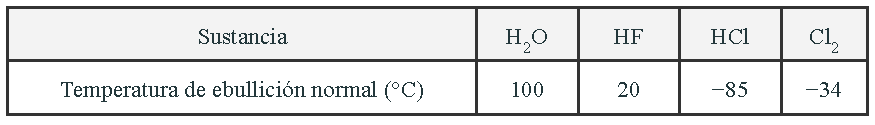
\includegraphics[width=0.65\linewidth]{FigurasSVG/UD3_Enlace_Quimico/pdf/UD3_E02_tabla_ebullicion.pdf}
        \caption{}
        \label{fig:tablaejercicios}
    \end{figure}

    \begin{solu}

%        \begin{figure}[H]
%            \centering
%            \includegraphics[scale=.5]{images/imagesUD3EnlaceQuimico/UD3_Problemas/evauclm12.png}
%        \end{figure}

        \begin{enumerate}[label=\letraminuscula]
            \item El HF es una molécula muy polar en la que el H está unido a un átomo muy electronegativo y pequeño (F), lo que le permite formar \textbf{enlaces de hidrógeno} entre sus moléculas. El HCl, aunque también es polar, no puede formar enlaces de H (el Cl no es lo bastante electronegativo ni pequeño) y solo presenta fuerzas dipolo-dipolo, más débiles. Por eso el punto de ebullición del HF es mayor.

            \item El \ch{H2O} forma \textbf{enlaces de hidrógeno} (además puede formar hasta dos por molécula, ya que tiene dos pares no enlazantes y dos H), mientras que el \ch{Cl2} es una molécula apolar que solo presenta débiles fuerzas de dispersión de London. Por ello, el punto de ebullición del \ch{H2O} es mucho mayor que el del \ch{Cl2}.

            \item Aunque el HCl es una molécula polar (fuerzas dipolo-dipolo) y el \ch{Cl2} es apolar (solo dispersión de London), el \ch{Cl2} tiene muchos más electrones y mayor masa molar que el HCl, lo que genera fuerzas de dispersión más intensas que compensan la ausencia de dipolo permanente. Por eso el punto de ebullición del HCl es menor que el del \ch{Cl2}.

            \item De las cuatro sustancias, el \ch{H2O} presentará el mayor punto de fusión, ya que es la que forma la red de enlaces de hidrógeno más extensa y fuerte (cada molécula puede establecer hasta cuatro enlaces de H con sus vecinas).
        \end{enumerate}
    \end{solu}
\end{exerciseEVAU}

\begin{exerciseEVAU}
    \textbf{2020} Para las siguientes sustancias: \ch{Br2}, \ch{NaCl}, \ch{H2O} y Fe: a) Explicar el tipo de enlace que presentan. b) Indicar el tipo de interacción que debe romperse para fundir cada compuesto.c) ¿Cuál de ellas tendrá un menor punto de fusión? d) Razonar qué compuesto(s) conducirá(n) la corriente en estado sólido, cuál(es) lo hará(n) en estado fundido y cuál(es) no conducirá(n) la corriente eléctrica en ningún caso.


    \begin{solu}

%        \begin{figure}[H]
%            \centering
%            \includegraphics[scale=.5]{images/imagesUD3EnlaceQuimico/UD3_Problemas/evauclm13.png}
%            \includegraphics[scale=.5]{images/imagesUD3EnlaceQuimico/UD3_Problemas/evauclm13b.png}
%        \end{figure}

        \begin{enumerate}[label=\letraminuscula]
            \item \ch{Br2}: molécula \textbf{covalente} apolar. \ch{NaCl}: \textbf{iónico}. \ch{H2O}: molécula \textbf{covalente} polar. Fe: \textbf{metálico}.

            \item Para fundir cada sustancia hay que romper las interacciones \emph{entre} unidades: \ch{Br2} $\to$ fuerzas de dispersión de London; \ch{NaCl} $\to$ atracciones electrostáticas de la red iónica; \ch{H2O} $\to$ enlaces de hidrógeno (y dipolo-dipolo); Fe $\to$ enlace metálico.

            \item El \ch{Br2} tiene el \textbf{menor punto de fusión}, ya que las fuerzas de dispersión de London entre sus moléculas apolares son mucho más débiles que la red iónica del NaCl, los enlaces de H del agua o el enlace metálico del Fe.

            \item El Fe \textbf{conduce en estado sólido} (enlace metálico, electrones deslocalizados libres en todo momento). El NaCl \textbf{no conduce en sólido, pero sí fundido} (o en disolución), ya que solo así los iones quedan libres para desplazarse. El \ch{Br2} y el \ch{H2O} (pura) \textbf{no conducen la corriente en ningún caso}, al ser sustancias covalentes sin iones ni electrones libres.
        \end{enumerate}
    \end{solu}
\end{exerciseEVAU}

\begin{exerciseEVAU}
    \textbf{2020} Explica razonadamente los siguientes hechos: a) El cloruro de sodio tiene un punto de fusión de 801 ºC,
    mientras que el cloro es un gas a temperatura ambiente. b) El metanol es un compuesto muy soluble en agua, mientras que el metano no lo es.
    c) El hierro y el yodo son sólidos a temperatura ambiente; pero el hierro conduce la corriente eléctrica, mientras que el yodo no. d) El cloruro de magnesio es más duro que el cloruro de calcio.

    \begin{solu}

%        \begin{figure}[H]
%            \centering
%            \includegraphics[scale=.5]{images/imagesUD3EnlaceQuimico/UD3_Problemas/evauclm15.png}
%        \end{figure}

        \begin{enumerate}[label=\letraminuscula]
            \item El NaCl es un compuesto \textbf{iónico}, con una red cristalina muy estable mantenida por fuertes fuerzas electrostáticas (alta energía de red), lo que requiere mucha energía para fundirlo. El \ch{Cl2} es una molécula \textbf{covalente apolar} en la que solo actúan débiles fuerzas de dispersión de London entre moléculas, por lo que es gas a temperatura ambiente.

            \item El metanol (\ch{CH3OH}) tiene un grupo --OH capaz de formar \textbf{enlaces de hidrógeno} con el agua, lo que lo hace muy soluble (miscible). El metano (\ch{CH4}) es una molécula apolar, sin capacidad de interaccionar favorablemente con el agua polar, por lo que es prácticamente insoluble.

            \item El Fe tiene \textbf{enlace metálico}: sus electrones de valencia están deslocalizados formando una nube libre de moverse, lo que le confiere conductividad eléctrica. El \ch{I2} es un sólido \textbf{covalente molecular} unido por fuerzas de dispersión de London; sus electrones están localizados en enlaces covalentes y pares solitarios, sin electrones libres, por lo que no conduce la corriente.

            \item El \(\text{Mg}^{2+}\) tiene menor radio iónico que el \(\text{Ca}^{2+}\), por lo que en el \ch{MgCl2} la distancia interiónica es menor y la atracción electrostática (energía de red) es mayor que en el \ch{CaCl2}. Una energía de red mayor implica una red cristalina más fuerte y, por tanto, un compuesto más duro. Por eso el \ch{MgCl2} es más duro que el \ch{CaCl2}.
        \end{enumerate}
    \end{solu}
\end{exerciseEVAU}
\begin{exerciseEVAU}
    \textbf{2021} Sean las moléculas \formula{NH3}, \formula{SO2} y \formula{CO2} a) Deduzca la estructura de Lewis de cada una de ellas. b) Describa la geometría de estas moléculas indicando la hibridación del átomo central. c) Indique el tipo de enlaces $\sigma$/ $\pi$ que se dan en estas moléculas. d) Comente la polaridad de cada molécula.

    \begin{solu}

%        \begin{figure}[H]
%            \centering
%            \includegraphics[scale=.5]{images/imagesUD3EnlaceQuimico/UD3_Problemas/evauclm16a.png}
%            \includegraphics[scale=.5]{images/imagesUD3EnlaceQuimico/UD3_Problemas/evauclm16b.png}
%        \end{figure}

        \begin{enumerate}[label=\letraminuscula]
            \item Las estructuras de Lewis se muestran en la imagen: \ch{NH3} con tres enlaces sencillos N--H y un par no enlazante sobre el N; \ch{SO2} con un doble enlace S=O y un enlace sencillo S--O (estructura resonante) y un par no enlazante sobre el S; \ch{CO2} con dos dobles enlaces \ch{O=C=O}.

            \item \textbf{\ch{NH3}}: tipo \(AB_3E\), geometría \textbf{pirámide trigonal}, hibridación del N: \(\bm{sp^3}\).

            \textbf{\ch{SO2}}: tipo \(AB_2E\), geometría \textbf{angular}, hibridación del S: \(\bm{sp^2}\).

            \textbf{\ch{CO2}}: tipo \(AB_2\), geometría \textbf{lineal}, hibridación del C: \(\bm{sp}\).

            \item \textbf{\ch{NH3}}: 3 enlaces \(\sigma\), sin enlaces \(\pi\). \textbf{\ch{SO2}}: 2 enlaces \(\sigma\) y 1 enlace \(\pi\) deslocalizado entre los dos enlaces S--O. \textbf{\ch{CO2}}: 2 enlaces \(\sigma\) y 2 enlaces \(\pi\).

            \item \textbf{\ch{NH3}}: geometría piramidal asimétrica $\Rightarrow$ \textbf{polar}. \textbf{\ch{SO2}}: geometría angular asimétrica $\Rightarrow$ \textbf{polar}. \textbf{\ch{CO2}}: geometría lineal simétrica, los momentos dipolares se cancelan $\Rightarrow$ \textbf{apolar}.
        \end{enumerate}
    \end{solu}
\end{exerciseEVAU}


\begin{exerciseEVAU}
    \textbf{2021} Justifique, en términos del enlace químico, por qué el \formula{H2O} es un líquido a presión y temperatura ambiente mientras que el \formula{H2S} es un gas en las mismas condiciones. b) Razone que tienen en común los siguientes átomos e iones: \formula{Cl^-}, \formula{Ar} y \formula{K^-}
    \datos{} Z (Cl) =17; Z (Ar) = 18; Z (K) = 19.

    \begin{solu}

%        \begin{figure}[H]
%            \centering
%            \includegraphics[scale=.5]{images/imagesUD3EnlaceQuimico/UD3_Problemas/evauclm17.png}
%        \end{figure}

        El O es mucho más electronegativo y pequeño que el S, lo que permite que las moléculas de \ch{H2O} formen \textbf{enlaces de hidrógeno} entre sí, una interacción intermolecular fuerte que exige mucha energía para separar las moléculas (de ahí que el agua sea líquida a temperatura ambiente). El \ch{H2S}, con un átomo central más grande y menos electronegativo, solo presenta fuerzas dipolo-dipolo y de dispersión, mucho más débiles, por lo que es gaseoso en las mismas condiciones.

        b) (Se entiende el ion del K como \ch{K+}, ya que un anión \ch{K-} no es una especie habitual en química básica). Las especies \ch{Cl-} (\(17+1=18\) electrones), \ch{Ar} (\(18\) electrones) y \ch{K+} (\(19-1=18\) electrones) son \textbf{isoelectrónicas}: todas tienen 18 electrones y la misma configuración electrónica, \( 1s^22s^22p^63s^23p^6 \), la del gas noble Ar.
    \end{solu}
\end{exerciseEVAU}
\begin{exerciseEVAU}
    Considere las moléculas \formula{BF3} y \formula{NH3}. a) Escriba su estructura de Lewis. b) Indique su geometría molecular utilizando la teoría de repulsión de pares de electrones de la capa de valencia. c) Indique cuál es la hibridación del átomo central de cada una de ellas. d) Explique la polaridad de ambas moléculas.

    \begin{solu}
        \begin{enumerate}[label=\letraminuscula]
            \item \textbf{\ch{BF3}}: el B (3 e\textsuperscript{-} de valencia) forma tres enlaces sencillos con los tres F, sin par no enlazante (sexteto sobre el B).

            \textbf{\ch{NH3}}: el N (5 e\textsuperscript{-} de valencia) forma tres enlaces sencillos con los tres H y le queda un par no enlazante.

            \item \textbf{\ch{BF3}}: 3 pares enlazantes, 0 no enlazantes $\Rightarrow$ tipo \(AB_3\), geometría \textbf{trigonal plana}.

            \textbf{\ch{NH3}}: 3 pares enlazantes, 1 no enlazante $\Rightarrow$ tipo \(AB_3E\), geometría \textbf{pirámide trigonal}.

            \item El B en \ch{BF3}, con tres pares de electrones a su alrededor dispuestos en un plano, presenta hibridación \(\bm{sp^2}\).

            El N en \ch{NH3}, con cuatro pares de electrones a su alrededor (3 enlazantes + 1 no enlazante) dispuestos tetraédricamente, presenta hibridación \(\bm{sp^3}\).

            \item \textbf{\ch{BF3}}: los enlaces B--F son polares, pero la simetría trigonal plana hace que los momentos dipolares se cancelen $\Rightarrow$ \textbf{molécula apolar}.

            \textbf{\ch{NH3}}: los enlaces N--H son polares y, debido a la geometría piramidal (asimétrica, con un par no enlazante que refuerza el momento dipolar resultante), los momentos dipolares no se cancelan $\Rightarrow$ \textbf{molécula polar}.
        \end{enumerate}
    \end{solu}
\end{exerciseEVAU}


\begin{exerciseEVAU}
    \textbf{2020} a) La propanona es la cetona más sencilla. a.1) Escribir la fórmula e indicar los enlaces \(\sigma\) y \(\pi\) que forma el átomo de carbono del grupo funcional. a.2) ¿Qué hibridación de los átomos de C puede explicar la estructura de la molécula? a.3) ¿Es una molécula polar? b) Dados los compuestos: ácido 2-hidroxipropanoico, 2-clorobutano y 1-aminoprop-1-eno b.1) Escribir su fórmula semidesarrollada. b.2) ¿Presentan isomería óptica? b.3) ¿Presentan isomería geométrica? Razonar las respuestas.

    \begin{solu}

%        \begin{figure}[H]
%            \centering
%            \includegraphics[scale=.5]{images/imagesUD3EnlaceQuimico/UD3_Problemas/evauclm19.png}
%            \includegraphics[scale=.5]{images/imagesUD3EnlaceQuimico/UD3_Problemas/evauclm19b.png}
%        \end{figure}

        \begin{enumerate}[label=\letraminuscula]
            \item[a.1)] La propanona es \ch{CH3-CO-CH3}. El carbono del grupo carbonilo forma 2 enlaces \(\sigma\) con los dos grupos metilo y, con el oxígeno, un doble enlace C=O formado por 1 enlace \(\sigma\) y 1 enlace \(\pi\).

            \item[a.2)] El carbono carbonílico, rodeado de 3 grupos de electrones (2 enlaces \ch{C-C} y 1 doble enlace C=O), tiene hibridación \(\bm{sp^2}\); los carbonos de los grupos metilo tienen hibridación \(\bm{sp^3}\).

            \item[a.3)] Sí, es una \textbf{molécula polar}: el doble enlace C=O es muy polar (el O es mucho más electronegativo) y la geometría trigonal plana alrededor del carbono carbonílico no permite que ese momento dipolar se cancele con los débiles enlaces C--C.

            \item[b.1)] Ácido 2-hidroxipropanoico (ácido láctico): \ch{CH3-CH(OH)-COOH}. 2-clorobutano: \ch{CH3-CHCl-CH2-CH3}. 1-aminoprop-1-eno: \ch{CH3-CH=CH-NH2}.

            \item[b.2)] El ácido 2-hidroxipropanoico y el 2-clorobutano presentan \textbf{isomería óptica}, ya que ambos tienen un átomo de carbono asimétrico (unido a cuatro sustituyentes distintos): el C2 en cada caso. El 1-aminoprop-1-eno no tiene ningún carbono asimétrico, por lo que \textbf{no presenta isomería óptica}.

            \item[b.3)] Solo el 1-aminoprop-1-eno presenta \textbf{isomería geométrica} (cis-trans), ya que tiene un doble enlace C=C con dos sustituyentes distintos en cada carbono del doble enlace (H/CH3 en un extremo y H/NH2 en el otro), lo que permite las formas cis y trans. Los otros dos compuestos no tienen dobles enlaces C=C y, por tanto, no presentan este tipo de isomería.
        \end{enumerate}
    \end{solu}
\end{exerciseEVAU}
\begin{exerciseEVAU}
    \textbf{ 2020} El propino es un hidrocarburo insaturado. a) Formula el propino y representa el diagrama de Lewis de la molécula. b) ¿Qué hibridación puede explicar los enlaces de los átomos de carbono? c) Escribe la reacción química del propino con bromo en proporción molar 1:1; indica de qué tipo es y nombra el compuesto orgánico formado. d) ¿Cómo afecta la reacción anterior a la hibridación del carbono?

    \begin{solu}

%        \begin{figure}[H]
%            \centering
%            \includegraphics[scale=.5]{images/imagesUD3EnlaceQuimico/UD3_Problemas/evauclm20.png}
%        \end{figure}

        \begin{enumerate}[label=\letraminuscula]
            \item El propino es \ch{HC} \(\equiv\) \ch{C-CH3}. Diagrama de Lewis: triple enlace entre C1 y C2 (cada uno con un par de electrones compartidos triple), C2 unido por enlace sencillo a C3 (\ch{CH3}), y el H terminal unido a C1.

            \item El C1 y el C2 (unidos por el triple enlace) están rodeados de solo 2 grupos de electrones, por lo que tienen hibridación \(\bm{sp}\). El C3 (\ch{CH3}), con cuatro enlaces sencillos, tiene hibridación \(\bm{sp^3}\).

            \item La adición de \ch{Br2} en proporción 1:1 al triple enlace es una \textbf{reacción de adición electrófila}. El \ch{Br2} se adiciona sobre el triple enlace, transformándolo en un doble enlace:
            \begin{center}
                \ch{HC} \(\equiv\) \ch{C-CH3 + Br2 -> CHBr=CBr-CH3}
            \end{center}
            El compuesto orgánico formado es el \textbf{1,2-dibromoprop-1-eno}.

            \item Los dos carbonos que reaccionan (C1 y C2), que partían de hibridación \(sp\) (triple enlace), pasan a tener hibridación \(\bm{sp^2}\) al quedar unidos por un doble enlace tras la adición.
        \end{enumerate}
    \end{solu}
\end{exerciseEVAU}

\begin{exerciseEVAU}
    \textbf{ 2018 } Justifica en términos del enlace químico los siguientes hechos: a) Los metales son dúctiles y maleables, pero los sólidos iónicos no. b) A presión y temperatura ambiente, el cloro (\ch{Cl2}) es un gas, mientras que el bromo (\ch{Br2}) es un líquido.

    \begin{solu}

%        \begin{figure}[H]
%            \centering
%            \includegraphics[scale=.5]{images/imagesUD3EnlaceQuimico/UD3_Problemas/evauclm20nuevo.png}
%        \end{figure}

        \begin{enumerate}[label=\letraminuscula]
            \item En el enlace metálico, los cationes metálicos están rodeados de una nube de electrones deslocalizados que no pertenecen a ningún ion en particular. Al aplicar una fuerza, las capas de cationes pueden deslizarse unas sobre otras sin romper el enlace, ya que la nube electrónica se reajusta y sigue rodeándolos: por eso los metales son dúctiles y maleables. En un sólido iónico, en cambio, cada ion ocupa una posición fija en la red y está unido a sus vecinos de carga opuesta por atracción electrostática; al desplazar una capa, iones de igual carga quedan enfrentados y se repelen fuertemente, lo que fractura el cristal.

            \item Tanto el \ch{Cl2} como el \ch{Br2} son moléculas apolares que solo interaccionan mediante fuerzas de dispersión de London, cuya intensidad aumenta con el tamaño y el número de electrones de la molécula. El \ch{Br2} tiene más electrones y mayor masa molar que el \ch{Cl2}, por lo que sus fuerzas de dispersión son más intensas, dando lugar a un punto de ebullición mayor: por eso el \ch{Br2} es líquido y el \ch{Cl2} gaseoso a temperatura y presión ambiente.
        \end{enumerate}
    \end{solu}
\end{exerciseEVAU}

\begin{exerciseEVAU}
    \textbf{ 2018 } Justifica la certeza o falsedad de las siguientes afirmaciones: a) Los iones \ch{S\mch[2]} y \ch{Ca\pch[2]} son isoelectrónicos. b) Arrancar un electrón a un átomo de K cuesta menos energía que arrancarlo a uno de Cs. c) El átomo de Fe tiene dos electrones desapareados. d) El enlace de la molécula de HF es más polar que el de la molécula de HI.

    \datos{} Números atómicos: F=9; S=16; K=19; Ca=20; Fe=26; I=53; Cs=55.

    \begin{solu}

%        \begin{figure}[H]
%            \centering
%            \includegraphics[scale=.5]{images/imagesUD3EnlaceQuimico/UD3_Problemas/evauclm21.png}
%        \end{figure}

        \begin{enumerate}[label=\letraminuscula]
            \item \textbf{Verdadero}. El \ch{S^{2-}} tiene \(16+2=18\) electrones y el \ch{Ca^{2+}} tiene \(20-2=18\) electrones; ambos comparten la configuración \( 1s^22s^22p^63s^23p^6 \), luego son isoelectrónicos.

            \item \textbf{Falso}. El K (periodo 4) tiene mayor energía de ionización que el Cs (periodo 6), ya que el radio atómico del Cs es mucho mayor (más capas de apantallamiento), lo que hace que su electrón de valencia esté menos atraído por el núcleo. Por tanto, arrancar un electrón cuesta \emph{más} energía en el K que en el Cs.

            \item \textbf{Falso}. La configuración electrónica del Fe es \([\text{Ar}]3d^64s^2\). Según la regla de Hund, los 6 electrones del subnivel \(3d\) (5 orbitales) se distribuyen: los 5 primeros orbitales reciben un electrón cada uno (5 desapareados) y el sexto electrón se aparea en el primer orbital. Por tanto, el Fe tiene \textbf{4 electrones desapareados}, no 2.

            \item \textbf{Verdadero}. La diferencia de electronegatividad entre H y F es mayor que entre H e I (el F es mucho más electronegativo que el I), por lo que el enlace H--F es más polar que el H--I.
        \end{enumerate}
    \end{solu}
\end{exerciseEVAU}
\begin{exerciseEVAU}

    \textbf{ 2018 } Sólo UNA de las siguientes afirmaciones es CORRECTA. Identifícala razonando tu respuesta. a) Los metales son malos conductores de la electricidad. b) Todos los compuestos iónicos son sólidos. c) La unión de un metal con un no metal se produce por enlace covalente. d) Los compuestos iónicos no se disuelven en agua.

    \begin{solu}

%        \begin{figure}[H]
%            \centering
%            \includegraphics[scale=.5]{images/imagesUD3EnlaceQuimico/UD3_Problemas/evauclm22.png}
%        \end{figure}

        La afirmación correcta es la \textbf{b) Todos los compuestos iónicos son sólidos} (a temperatura ambiente, dada su elevada energía de red).

        Las otras son falsas: a) los metales son \emph{buenos} conductores de la electricidad (enlace metálico, electrones deslocalizados); c) la unión de un metal con un no metal da lugar a enlace \textbf{iónico}, no covalente; d) muchos compuestos iónicos, como el NaCl, \textbf{sí se disuelven} en agua.
    \end{solu}
\end{exerciseEVAU}

\begin{exerciseEVAU}
    \textbf{ 2017 } Para los elementos con Z = 9, 12, 16 y 28, a) Indica a qué grupo del sistema periódico pertenece cada uno de ellos. b) ¿Cuál de los cuatro elementos tendrá mayor afinidad electrónica? c) ¿Alguna combinación binaria entre ellos tendrá carácter iónico? d) ¿Cuál o cuáles de los cuatro elementos podrán formar enlace metálico?


    \begin{solu}

%        \begin{figure}[H]
%            \centering
%            \includegraphics[scale=.5]{images/imagesUD3EnlaceQuimico/UD3_Problemas/evauclm23.png}
%        \end{figure}

        \begin{enumerate}[label=\letraminuscula]
            \item \(Z=9\): \(1s^22s^22p^5\), grupo 17 (\textbf{F}, halógenos). \(Z=12\): \(1s^22s^22p^63s^2\), grupo 2 (\textbf{Mg}, alcalinotérreos). \(Z=16\): \(1s^22s^22p^63s^23p^4\), grupo 16 (\textbf{S}, anfígenos). \(Z=28\): \([\text{Ar}]3d^84s^2\), grupo 10 (\textbf{Ni}, metales de transición).

            \item El \(F\) (\(Z=9\)) tendrá la \textbf{mayor afinidad electrónica}, ya que los halógenos, pequeños y muy electronegativos, son los elementos con mayor tendencia a captar un electrón.

            \item Sí: por ejemplo, la combinación entre Mg (metal) y F o S (no metales) presenta gran diferencia de electronegatividad, dando lugar a compuestos de carácter \textbf{iónico} (\ch{MgF2} o \ch{MgS}).

            \item El Mg y el Ni son los dos elementos metálicos, por lo que ambos pueden formar enlace metálico.
        \end{enumerate}
    \end{solu}
\end{exerciseEVAU}

\begin{exerciseEVAU}
    \textbf{ 2017 } Formula el compuesto 2-propenol (propen-2-ol, 1-propen-2-ol) y responde a las siguientes cuestiones: a) ¿Cuál es la hibridación de los átomos de carbono 2 y 3? b) De todos los enlaces de esta molécula, cuál es el enlace más polar? Indica, además, un enlace sigma (\(\sigma\)) y un enlace pi (\(\pi\)). c) Formula y nombra un isómero de función del 2-propenol.

    \begin{solu}

%        \begin{figure}[H]
%            \centering
%            \includegraphics[scale=.5]{images/imagesUD3EnlaceQuimico/UD3_Problemas/evauclm24.png}
%        \end{figure}

        El 2-propenol es \ch{CH2=C(OH)-CH3} (\(\text{C1}{=}\text{CH}_2\), \(\text{C2}{=}\text{C(OH)}\), \(\text{C3}{=}\text{CH}_3\)).

        \begin{enumerate}[label=\letraminuscula]
            \item El C2, que forma parte del doble enlace \ch{C1=C2} y está además unido al --OH, está rodeado de 3 grupos de electrones, por lo que tiene hibridación \(\bm{sp^2}\). El C3 (\ch{CH3}), con cuatro enlaces sencillos, tiene hibridación \(\bm{sp^3}\).

            \item El enlace más polar de la molécula es el \textbf{O--H} (mayor diferencia de electronegatividad entre O y H que entre C y O). Un ejemplo de enlace \(\sigma\) es el enlace \ch{C2-C3}; un ejemplo de enlace \(\pi\) es el que forma parte del doble enlace \ch{C1=C2}.

            \item Un isómero de función del 2-propenol (fórmula \ch{C3H6O}) es la \textbf{propanona (acetona)}, \ch{CH3-CO-CH3} (o también el propanal, \ch{CH3-CH2-CHO}): mismo número y tipo de átomos, pero con función cetona (o aldehído) en lugar de enol.
        \end{enumerate}
    \end{solu}
\end{exerciseEVAU}

\begin{exerciseEVAU}
    \textbf{2017}. Sólo UNA de las siguientes afirmaciones es FALSA. Identifícala razonando todas tus respuestas. a) El cloruro de potasio (KCl) conduce la electricidad en estado fundido. b) A temperatura ambiente, todas las sustancias covalentes son gases. c) El diamante, siendo una sustancia covalente, tiene un punto de fusión muy alto. d) Todos los metales son buenos conductores de la electricidad.
    \begin{solu}
%        \begin{figure}[H]
%            \centering
%            \includegraphics[scale=.5]{images/imagesUD3EnlaceQuimico/UD3_Problemas/evauclm25.png}
%        \end{figure}

        La afirmación \textbf{falsa} es la \textbf{b) A temperatura ambiente, todas las sustancias covalentes son gases}: existen sustancias covalentes moleculares sólidas (como el diamante o el propio azúcar) y líquidas (como el agua), no solo gaseosas.

        Las otras son verdaderas: a) el KCl, compuesto iónico, conduce fundido (los iones quedan libres para moverse); c) el diamante, sólido covalente atómico con una red tridimensional de enlaces C--C muy fuertes, tiene un punto de fusión muy elevado; d) todos los metales, gracias al enlace metálico, son buenos conductores de la electricidad.
    \end{solu}
\end{exerciseEVAU}

% \newpage

% \begin{table}[H]
%     \centering
%     \begin{tblr}{|Q[c,m]|Q[c,m]|}
%         \hline
%         {\textbf{Geometría}                                                                                                   \\ (cuando los átomos unidos al átomo central son iguales)} & \textbf{Polaridad}\\
%         \hline
%         {\includegraphics[scale=.5]{images/imagesUD3EnlaceQuimico/UD3_Problemas/lineal.png}  Lineal}                                                  & Apolar \\
%         \hline
%         {\includegraphics[scale=0.5]{images/imagesUD3EnlaceQuimico/UD3_Problemas/trigonal.png}  Trigonal plana (triangular)}                          & Polar  \\
%         \hline
%         {\includegraphics[scale=0.5]{images/imagesUD3EnlaceQuimico/UD3_Problemas/angular.png} Angular}                                                & Polar  \\
%         \hline
%         {\includegraphics[scale=0.5]{images/imagesUD3EnlaceQuimico/UD3_Problemas/tetraedrica.png} Tetraédrica }                                       & Apolar \\
%         \hline
%         {\includegraphics[scale=.5]{images/imagesUD3EnlaceQuimico/UD3_Problemas/piramidetrigonal.png}  Pirámide trigonal}                             & Polar  \\
%         \hline
%         {\includegraphics[scale=.5]{images/imagesUD3EnlaceQuimico/UD3_Problemas/bipiramidetrigonal.png}  Bipirámide trigonal (bipirámide triangular)} & Polar  \\
%         \hline
%         {\includegraphics[scale=.5]{images/imagesUD3EnlaceQuimico/UD3_Problemas/tetraedricadistorsionada.png} Tetraédrica distorsionada }             & Polar  \\
%         \hline
%         {\includegraphics[scale=.5]{images/imagesUD3EnlaceQuimico/UD3_Problemas/enformadeT.png} En forma de T}                                        & Polar  \\
%         \hline
%         {\includegraphics[scale=.5]{images/imagesUD3EnlaceQuimico/UD3_Problemas/octaedrica.png}  Octaédrica}                                          & Apolar \\
%         \hline
%         {\includegraphics[scale=.5]{images/imagesUD3EnlaceQuimico/UD3_Problemas/piramidalcuadrada.png}  Pirámide cuadrada}                            & Polar  \\
%         \hline
%         {\includegraphics[scale=.5]{images/imagesUD3EnlaceQuimico/UD3_Problemas/planacuadrada.png}  Plano cuadrada}                                   & Apolar \\
%         \hline
%     \end{tblr}
% \end{table}

% \begin{table}[H]
%     \centering
%     \begin{tblr}{|Q[c,m]|Q[c,m]|Q[c,m]|Q[c,m]|Q[c,m]|}
%         \hline
%         {\textbf{nº total de}                                                                                                                                                           \\ \textbf{pares de \el}} & {\textbf{nº total de pares} \\ \textbf{de \el enlazantes}} & {\textbf{nº total de pares} \\ \textbf{de \el no enlazantes}} &\textbf{Geometría} & \textbf{Ejemplo}\\
%         \hline
%         2                  & 2 & 0 & {\includegraphics[scale=.5]{images/imagesUD3EnlaceQuimico/UD3_Problemas/lineal.png}                                                      Lineal}                       & \ch{BeF2}  \\
%         \hline
%         \SetCell[r=2]{m} 3 & 3 & 0 & {\includegraphics[scale=.5]{images/imagesUD3EnlaceQuimico/UD3_Problemas/trigonal.png}                                                     Trigonal plana (triangular)} & \ch{BeF2}  \\
%         \hline
%                            & 2 & 1 & {\includegraphics[scale=.5]{images/imagesUD3EnlaceQuimico/UD3_Problemas/angular.png} Angular   }                                                                       & \ch{SnCl2} \\
%         \hline
%         \SetCell[r=3]{m} 4 & 4 & 0 & {\includegraphics[scale=.5]{images/imagesUD3EnlaceQuimico/UD3_Problemas/tetraedrica.png} Tetraédrica }                                                                 & \ch{CH4}   \\
%         \hline
%                            & 3 & 1 & {\includegraphics[scale=.5]{images/imagesUD3EnlaceQuimico/UD3_Problemas/piramidetrigonal.png} Pirámide trigonal }                                                      & \ch{NH3}   \\
%         \hline
%                            & 2 & 2 & {\includegraphics[scale=.5]{images/imagesUD3EnlaceQuimico/UD3_Problemas/angularb.png} Angular }                                                                        & \ch{H2O}   \\
%         \hline
%         \SetCell[r=4]{m} 5 & 5 & 0 & {\includegraphics[scale=.5]{images/imagesUD3EnlaceQuimico/UD3_Problemas/bipiramidetrigonal.png} Bipirámide triangular}                                                 & \ch{PCl5}  \\
%         \hline
%                            & 4 & 1 & {\includegraphics[scale=.5]{images/imagesUD3EnlaceQuimico/UD3_Problemas/tetraedricadistorsionada.png} Tetraédrica distorsionada}                                       & \ch{SF4}   \\
%         \hline
%                            & 3 & 2 & {\includegraphics[scale=.5]{images/imagesUD3EnlaceQuimico/UD3_Problemas/enformadeT.png} En forma de T  }                                                               & \ch{ClF3}  \\
%         \hline
%                            & 2 & 3 & {\includegraphics[scale=.5]{images/imagesUD3EnlaceQuimico/UD3_Problemas/linealb.png} Lineal  }                                                                         & \ch{XeF2}  \\
%         \hline
%         \SetCell[r=3]{m}6  & 6 & 0 & {\includegraphics[scale=.5]{images/imagesUD3EnlaceQuimico/UD3_Problemas/octaedrica.png} Octaédrica}                                                                    & \ch{SF6}   \\
%         \hline
%                            & 5 & 1 & {\includegraphics[scale=.5]{images/imagesUD3EnlaceQuimico/UD3_Problemas/piramidalcuadrada.png} Pirámide cuadrada}                                                      & \ch{ICl5}  \\
%         \hline
%                            & 4 & 2 & {\includegraphics[scale=.5]{images/imagesUD3EnlaceQuimico/UD3_Problemas/planacuadrada.png} Plano cuadrada}                                                             & \ch{XeF4}  \\
%         \hline
%     \end{tblr}
% \end{table}




%----------------------------------------------------------------------------------------
%	PART
%----------------------------------------------------------------------------------------


    \part{Termodinámica}

%----------------------------------------------------------------------------------------
%	SECTIONING EXAMPLES CHAPTER
%----------------------------------------------------------------------------------------

    \chapterimage{orange4b.png} % Chapter heading image
    \chapterspaceabove{6.75cm} % Whitespace from the top of the page to the chapter title on chapter pages
    \chapterspacebelow{7.25cm} % Amount of vertical whitespace from the top margin to the start of the text on chapter pages

%------------------------------------------------


    \chapter{Termodinámica}

    \spacing{1.3}


\section{Introducción}


\begin{definition}[Termodin\'amica]
    Se denomina \textbf{termodinámica} a la parte de la física que estudia los intercambios de calor y trabajo que acompañan a los procesos fisicoquímicos; si estos son reacciones químicas, la parte de la ciencia que los estudia se denomina \textbf{termoquímica}
\end{definition}


\section{Termodinámica. Conceptos básicos}\label{sec:termodinamica.-conceptos-basicos}

\subsection{Equivalente mecánico del calor}\label{subsec:equivalente-mecanico-del-calor}

\textbf{James Prescott Joule} diseñó un dispositivo que permitía efectuar medidas muy precisas de la equivalencia entre el trabajo mecánico y el calor.

\begin{itemize}
    \item La caída de las pesas (trabajo mecánico) produce la fricción interna de las paletas con el agua (entra calor al sistema), lo que provoca un aumento de temperatura de esta.
    \item Joule demostró que, cuando entra \SI{1}{\calorie} de calor, las pesas hacen \num{4.184} unidades de trabajo mecánico que más tarde, y en su honor, se denominaron julios (\unit{\joule}).
\end{itemize}

Podemos decir, por tanto, que \(\SI{1}{\calorie} = \SI{4.18}{\joule}\)

\subsection{Sistema termodinámico}\label{subsec:sistema-termodinamico}

Se llama \textbf{sistema termodinámico} aquella parte del \textbf{universo} que aislamos para someterla a un estudio fisicoquímico.
Lo que rodea a este sistema recibe el nombre de \textbf{entorno}.

Según sea la relación entre sistema y entorno tendremos:

\begin{enumerate}[label=\numberballmDarkTeal]
        \item \textbf{Sistema abierto}.
        Intercambia materia y energía con el entorno.
        \item \textbf{Sistema cerrado}.
        Intercambia energía con el entorno, pero no materia.
        \item \textbf{Sistema aislado}.
        No intercambia materia ni energía con el entorno.
\end{enumerate}

\begin{figure}[H]
    \centering
    % [FIGURA ORIGINAL] \includegraphics[scale=.7]{images/imagesUD4Termidonamica/UD4_Teoria/sistemas}\label{fig:sistemas}
    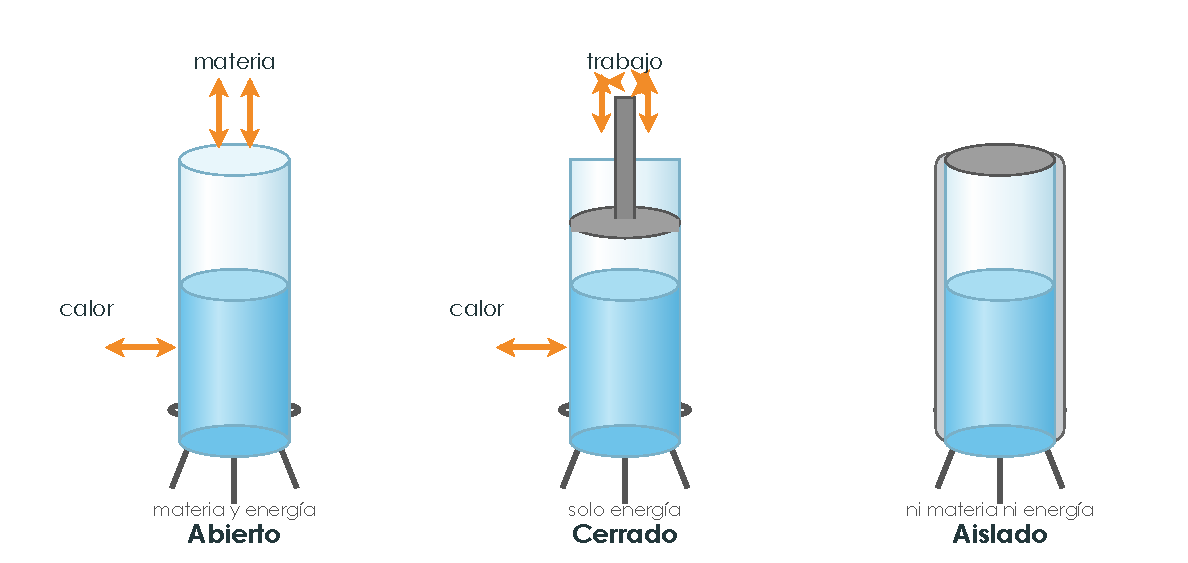
\includegraphics[width=0.75\linewidth]{FigurasSVG/UD4_Termodinamica/pdf/UD4_01_sistemas.pdf}\label{fig:sistemas}
\end{figure}

Para describir un sistema termodinámico es preciso conocer el valor de sus propiedades.
A estas propiedades / magnitudes se les conoce como \textbf{variables termodinámicas} como por ejemplo el volumen, temperatura, presión, composición etc.

Algunas variables dependen solo del estado en que se encuentra el sistema y no de cómo evolucionó para llegar a él, como el volumen, la presión o la temperatura.
A este tipo de variables se les denomina \textbf{variables de estado} o \textbf{funciones de estado}.

A las variables que dependen de como evoluciona el sistema se les conoce como \textbf{variables de transferencia} como puede ser el calor, trabajo, etc.

\subsection{Procesos termodinámicos}\label{subsec:procesos-termodinamicos}


\begin{definition}[Poceso termodinámico]
    Se denomina \textbf{proceso termodinámico} a la evolución seguida por un sistema cuando pasa de un estado inicial (\(p_0, T_0, V_0\)) a otro final (\(p_f, T_f, V_f\)).
\end{definition}


Estos procesos termodinámicos se clasifican en:

\begin{enumerate}[label=\numberballmDarkTeal]
        \item Atendiendo al sentido de la evolución:
        \begin{itemize}
            \item \textbf{Irreversibles}: si lo hacen en un único sentido.
            La mayor parte de los procesos son de este tipo:
            \begin{equation*}
                \ch{4 Fe + 3 O2 -> 2 Fe2O3}
            \end{equation*}
            \item \textbf{Reversibles}: si lo hacen a través de múltiples estados de equilibrio.
            \begin{equation*}
                \ch{N2 + 3 H2 <=> 2 NH3}
            \end{equation*}
        \end{itemize}
        \item Atendiendo a si en la evolución hay alguna variable de estado que permanezca constante:
        \begin{itemize}
            \item \textbf{Isobáricos}: si la presión no varía.
            La mayoría de las reacciones químicas se hacen a presión constante puesto que se realizan en recipientes abiertos.
            \item \textbf{Isocóricos}: si el volumen no varía.
            Ocurre en recipientes cerrados.
            \item \textbf{Isotérmicos}: si la temperatura no varía.
        \end{itemize}
\end{enumerate}


\section{Calor y trabajo en un proceso}\label{sec:calor-y-trabajo-en-un-proceso}

\subsection{Intercambio de calor en un proceso}\label{subsec:intercambio-de-calor-en-un-proceso}


\begin{definition}[Calor]
    Se define \textbf{calor} (\(\bm{Q}\)) como aquella energía en tránsito (intercambiada entre el sistema y su entorno) que produce cambios de temperatura o cambios de estado.
\end{definition}


El cálculo del calor variará si existen cambios de temperatura o cambios de estado:

\begin{itemize}
    \item Si existe cambio de temperatura:

    \begin{centeredequation}
        Q = m\ c_e\ \Delta T
    \end{centeredequation}

    Donde \(c_e\) es el llamado \textbf{calor específico} que nos dice la relación entre el calor agregado por unidad de masa y la variación de la temperatura que en ella se produce y es característico de cada sustancia.
    Sus unidades son \unit{\joule\per\kilo\g} o \unit{\calorie\per\g\per\celsius} y \(\Delta T\) es el incremento de temperatura experimentado.
    \item Si existe un cambio de estado:

    \begin{centeredequation}
        Q = m\ L_{\text{fus}} \qquad  Q = m\ L_{\text{vap}}
    \end{centeredequation}

    donde \(L_{\text{fus}}\) o \(L_{\text{vap}}\) son los llamados \textbf{calor latente de cambio de estado} siendo el primero para el cambio de sólido a líquido y el segundo de líquido a gas.
    Este calor latente de cambio de estado se define como la cantidad de calor que hay que suministrar a la unidad de masa de una sustancia para que, sin variar su temperatura, cambie de estado, midiéndose, por tanto, en \unit{\joule\per\kilo\g} o \unit{\calorie\per\g}
\end{itemize}

\subsection{Intercambio de trabajo en un proceso}\label{subsec:intercambio-de-trabajo-en-un-proceso}

Se define \textbf{trabajo} (\(\bm{W}\)) como aquella energía en tránsito que sucede a través de fuerzas y desplazamientos.
Su unidad sería \unit{\joule} o \unit{\atmosphere\litre}.

La relación del julio con el \unit{\atmosphere\litre}:
\begin{centeredequation}
    \SI{1}{\atmosphere\litre} = \SI{101300}{\pascal}\cdot \SI{e-3}{\cubic\metre} = \SI{101.3}{\joule}
\end{centeredequation}

Según el criterio de signos:

\begin{itemize}
    \item Si \(W<0\) el trabajo lo \textbf{realiza el sistema}.
    \item Si \(W>0\) el trabajo lo \textbf{realiza el entorno}.
\end{itemize}

En las reacciones químicas el trabajo está relacionado con las expansiones y compresiones.

\begin{itemize}
    \item El trabajo en una expansión:
    \begin{gather*}
        dW = -F\ dx = -p\ S\ dx = -p\ dV \separ
        W = - \int_{V_1}^{V_2} p\ dV
    \end{gather*}
    \item El trabajo en una compresión:
    \begin{gather*}
        dW = F\ dx = p\ S\ dx = p\ dV \separ
        W =  \int_{V_1}^{V_2} p\ dV
    \end{gather*}
\end{itemize}

Para resolver las integrales, es preciso conocer como varía la \(p\) en función del \(V\).
Según el tipo de proceso tendremos que:

\begin{itemize}
    \item \textbf{Isobáricos} (\(p = \text{cte}\))
    \begin{gather*}
        W = - \int_{V_1}^{V_2} p\ dV = - p \int_{V_1}^{V_2}  dV \separ
        W = -p\ (V_2 - V_1)
    \end{gather*}
    \begin{figure}[H]
        \centering
        % [FIGURA ORIGINAL] \includegraphics[scale=1]{images/imagesUD4Termidonamica/UD4_Teoria/trabajo_isobarico}\label{fig:trabajo-isobarico}
        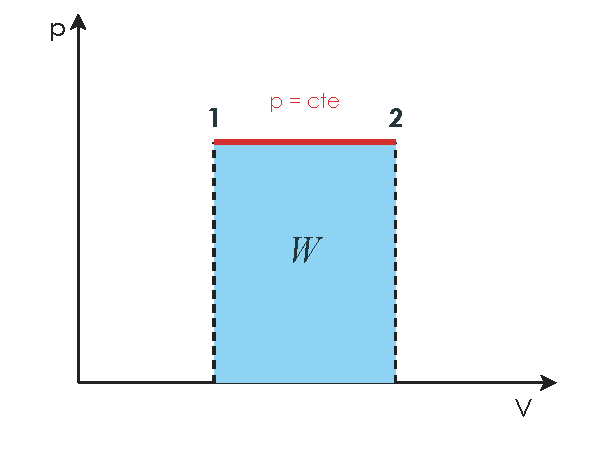
\includegraphics[width=0.45\linewidth]{FigurasSVG/UD4_Termodinamica/pdf/UD4_02_trabajo_isobarico.pdf}\label{fig:trabajo-isobarico}
    \end{figure}
    \item \textbf{Isotérmicos} (\(T = \text{cte}\))
    \begin{gather*}
        W = - \int_{V_1}^{V_2} p\ dV = - \int_{V_1}^{V_2} \dfrac{n\ R\ T}{V} \ dV = - n\ R\ T \int_{V_1}^{V_2} \dfrac{dV}{V} \separ
        W = -n\ R\ T\ ln\ \dfrac{V_2}{V_1}
    \end{gather*}
    \begin{figure}[H]
        \centering
        % [FIGURA ORIGINAL] \includegraphics[scale=1]{images/imagesUD4Termidonamica/UD4_Teoria/trabajo_isotermico}\label{fig:trabajo-isotermico}
        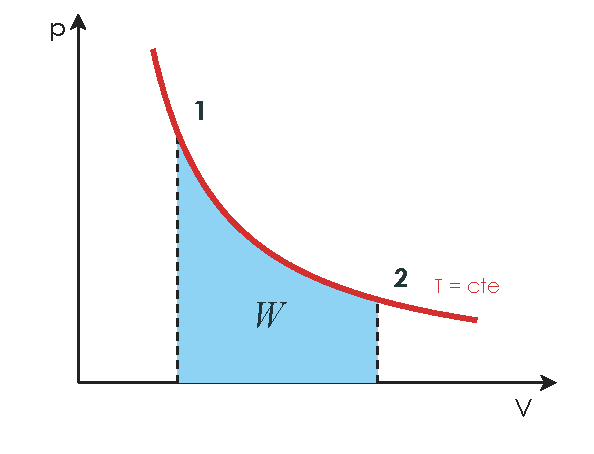
\includegraphics[width=0.45\linewidth]{FigurasSVG/UD4_Termodinamica/pdf/UD4_03_trabajo_isotermico.pdf}\label{fig:trabajo-isotermico}
    \end{figure}
    \item \textbf{Isocóricos} (\(V = \text{cte}\)).
    En este caso al no existir variación de volumen el \(V_2 = V_1\) y por tanto el trabajo será \(W = 0\)
    \begin{equation*}
        W = - \int_{V_1}^{V_2} p\ dV = 0
    \end{equation*}
    \begin{figure}[H]
        \centering
        % [FIGURA ORIGINAL] \includegraphics[scale=1]{images/imagesUD4Termidonamica/UD4_Teoria/trabajo_isocorico}\label{fig:trabajo-isocorico}
        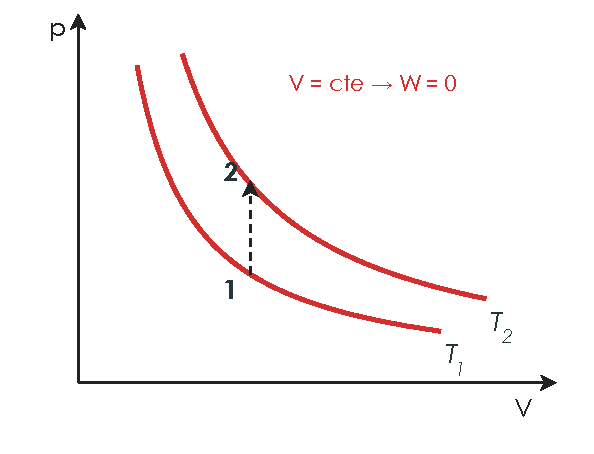
\includegraphics[width=0.45\linewidth]{FigurasSVG/UD4_Termodinamica/pdf/UD4_04_trabajo_isocorico.pdf}\label{fig:trabajo-isocorico}
    \end{figure}
\end{itemize}


\section{Primer principio de la termodinámica}\label{sec:primer-principio-de-la-termodinamica}

Cuando un sistema experimenta una transformación, suele intercambiar calor y trabajo con su entorno; el resultado es una variación de su \textbf{energía interna}

\begin{center}
    \begin{definition}[Energía Interna]
        La \textbf{energía interna} de un sistema es la suma de las energías de todas las partículas que lo forman.
        Se representa con la letra \(U\) y en el sistema internacional se mide en \textbf{julios}.
        Es una función de estado ya que su valor solo depende del estado en el que se encuentra el sistema.
    \end{definition}
\end{center}



\begin{figure}[H]
    \centering
    % [FIGURA ORIGINAL] \includegraphics[scale=1]{images/imagesUD4Termidonamica/UD4_Teoria/energia_interna}
    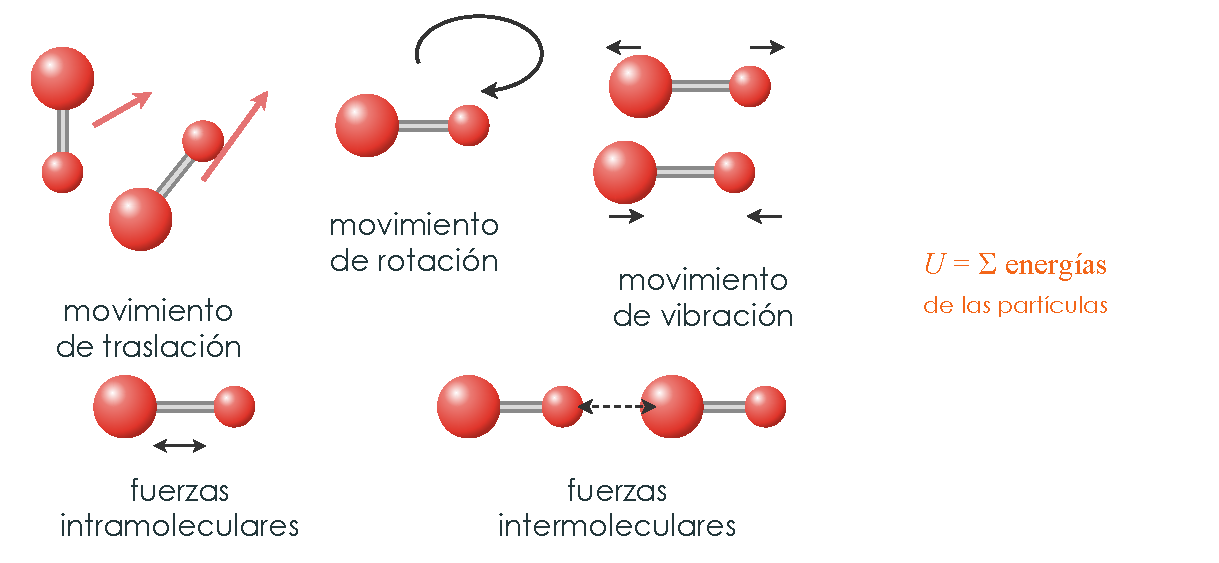
\includegraphics[width=0.8\linewidth]{FigurasSVG/UD4_Termodinamica/pdf/UD4_05_energia_interna.pdf}
    \caption{Representación de la energía interna}
    \label{fig:energia_interna}
\end{figure}

Las partículas de un sistema tienen energía cinética (por el movimiento de las moléculas) y energía potencial (por la atracción entre electrones y núcleos dentro de una molécula y las interacciones entre las moléculas).

\begin{ley}[Primer Principio de la Termodinámica]
    El \textbf{Primer principio de la Termodinámica} establece que, cuando un sistema evoluciona de un estado inicial a otro final, la variación que experimenta su energía interna coincide con la suma del calor y trabajo que intercambia con el entorno en esa transformación:
    \begin{centeredequation}
        \Delta U = Q + W
    \end{centeredequation}

\end{ley}


Si nos fijamos, este primer principio no es más que una conservación de la energía.

Es importante conocer los \textbf{criterios de signos} que recomienda la IUPAC para el calor y el trabajo que intercambia un sistema con su entorno.

\begin{itemize}
    \item Si se transfiere calor o trabajo desde el entorno al sistema consideraremos \(Q>0\) y \(W>0\).
    \item Si es el propio sistema el que cede calor o trabajo al entorno, entonces consideraremos \(Q<0\) y \(W<0\).
\end{itemize}

\begin{figure}[H]
    \centering
    % [FIGURA ORIGINAL] \includegraphics[scale=1]{images/imagesUD4Termidonamica/UD4_Teoria/criteriosdesignos}
    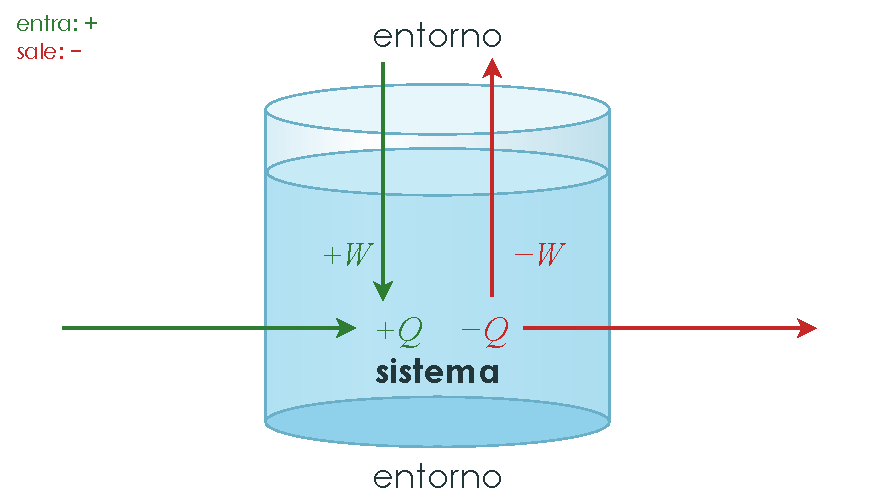
\includegraphics[width=0.6\linewidth]{FigurasSVG/UD4_Termodinamica/pdf/UD4_06_criterio_signos.pdf}
    \caption{Criterio de signos}
    \label{fig:cristerio-de-signos}
\end{figure}

\subsection{Aplicación del primer principio a diversos procesos termodinámicos}\label{subsec:aplicacion-del-primer-principio-a-diversos-procesos-termodinamicos.}

\begin{enumerate}[label=\numberballmDarkTeal]
        \item \textbf{Proceso isotérmico} (\(T = \text{cte}\)).
        En este caso, \(\Delta U = 0\) ya que la energía interna solo depende de la temperatura y, al ser esta constante, su variación es \num{0}.
        Si aplicamos el primer principio llegamos a la conclusión de que \(Q = - W\).
        \begin{gather*}
            \Delta U = Q + W \Rightarrow 0 = Q + W \separ
            Q = -W
        \end{gather*}
        \item \textbf{Proceso adiabático}.
        Es aquel en el que no hay intercambio de calor con el entorno (\(Q = 0\)). Aplicando el primer principio tendríamos:
        \begin{gather*}
            \Delta U = Q + W \Rightarrow \Delta U = 0 + W \separ
            \Delta U = W
        \end{gather*}
        Por lo tanto de aquí podemos determinar que si un gas se expande disminuirá su energía interna (\(\Delta U < 0\)) puesto que \(W < 0\).
        Si un gas se comprime aumentará su energía interna (\(\Delta U > 0\)) puesto que \(W > 0\).
        \item \textbf{Proceso isocórico} (\(V = \text{cte}\)).
        En este caso el trabajo será \(W = 0\) puesto que no hay cambio en el volumen (\(W = -p\ dV\)). Si aplicamos el primer principio tendremos que:
        \begin{gather*}
            \Delta U = Q + W \Rightarrow \Delta U = Q + 0 \separ
            \Delta U = Q
        \end{gather*}
        En este caso vemos como la variación de energía interna es igual al calor puesto en juego en el proceso.
        Por norma general en este caso se suele representar el calor como \(Q_V\) para indicar que es a volumen constante.
        \begin{centeredequation}
            \Delta U = Q_V
        \end{centeredequation}

        \item \textbf{Proceso isobárico} (\(p = \text{cte}\)).
        Aplicando el primer principio tendremos que:
        \begin{centeredequation}
            \Delta U = Q + W \Rightarrow \Delta U = Q_p - p\ \Delta V
        \end{centeredequation}

        Como vemos en este caso, el calor lo hemos denominado \(Q_p\) para indicar que estamos en un proceso a \(p = \text{cte}\).
\end{enumerate}


\section{Entalpía. Ecuaciones termoquímicas}\label{sec:entalpia.-ecuaciones-termoquimicas}

Por norma general, las reacciones químicas transcurren a presión constante.
Si aplicamos el primer principio a esta situación tendríamos que:
\begin{centeredequation}
    \Delta U = Q_p - p\ (V_2-V_1) \Rightarrow U_2-U_1 = Q_p - p\ (V_2-V_1)
\end{centeredequation}
Si reordenamos la expresión de manera que:
\begin{centeredequation}
(U_2 + pV_2) -  (U_1 + pV_1) = Q_p \label{eq:definicion_entalpia}
\end{centeredequation}

Podemos definir una función que denominamos \textbf{entalpía} y la representamos con la letra \(\bm{H}\) de la siguiente manera:
\begin{centeredequation}
    H = U + pV
\end{centeredequation}

De esta manera, la expresión de la ecuación~\eqref{eq:definicion_entalpia} quedará como:
\begin{centeredequation}
    Q_p = H_2 - H_1 = \Delta H
\end{centeredequation}


\begin{center}
    \begin{definition}[Entalp\'ia]
        Se denomina  \textbf{entalpía} de un sistema (\(H\)) a la magnitud suma de la energía interna y el producto de la presión por el volumen de dicho sistema \(H = U + pV\).
        Es una función de estado y su unidad es el julio.

        La entalpía, por tanto, representa el calor que intercambia con el entorno cuando el proceso se realiza a presión constante.
    \end{definition}
\end{center}

\subsection{Relación ente \texorpdfstring{\(\Delta U\)}{U} y \texorpdfstring{\(\Delta H\)}{H}}\label{subsec:relacion-ente-texorpdfstring{(delta-u)}{u}-y-texorpdfstring{(delta-h)}{h}}

Es posible establecer la relación entre la variación de entalpía y la de energía interna utilizando la propia definición de entalpía vista anteriormente.
\begin{centeredequation}
    H = U + pV \Rightarrow \Delta H = \Delta U + \Delta (pV)
\end{centeredequation}

\begin{itemize}
    \item Si en el sistema solo intervienen \textbf{sólidos} o \textbf{líquidos}, la presión y el volumen prácticamente no varían siendo, por tanto, el trabajo de expansión cero.
    En esos casos:
    \begin{gather}
        \Delta H = \Delta U \notag \separ
        Q_p = Q_v
    \end{gather}
    \item Si en el sistema intervienen \textbf{gases ideales}:
    \begin{gather}
        \Delta H = \Delta U + \Delta (nRT) = \Delta U + (\Delta n)RT \notag \separ
        Q_p = Q_v + (\Delta n) R T
    \end{gather}
\end{itemize}

\subsection{Ecuación termoquímica}\label{subsec:ecuacion-termoquimica}

La ecuación termoquímica es la ecuación química ajustada en la que, además de indicar el estado de agregación de todas las sustancias que intervienen y la presión y la temperatura a la que se realiza, hay que especificar la cantidad de calor intercambiado con el entorno.
\begin{centeredequation}
    \ch{1/2 N2 \gas{} + 1/2 O2 \gas{} -> NO \gas{}}\quad  \Delta H^0 = \energia[kj]{90.2}
\end{centeredequation}

Según el signo de este calor puesto en juego tendremos reacciones \textbf{endotérmicas} o \textbf{exotérmicas}

\begin{itemize}
    \item Si para pasar de reactivos a productos el sistema cede calor al entorno, el proceso se denomina \textbf{exotérmico} y \(\Delta H < 0\).
    \item Si para pasar de reactivos a productos el sistema absorbe calor del entorno, el proceso se llama \textbf{endotérmico} y \(\Delta H > 0\).
\end{itemize}

\subsection{Diagramas entálpicos}\label{subsec:diagramas-entalpicos}

Los diagramas entálpicos son la representación gráfica del contenido energético de los reactivos (\textbf{R}), los productos (\textbf{P})  y la variación de entalpía que ha sufrido el proceso.

\begin{center}
    \begin{endiagram}[
        x-label-text = {Tiempo de reacci\'on},
        y-label-text = {Energ\'ia},
        scale={1.2}
    ]
            \ENcurve{3,4,0}
            \ShowNiveaus[niveau={N1-1,N1-2,N1-3}]
            \node[below] at (N1-1) {R} ;
            \node[below] at (N1-3) {P} ;
            \ShowGain[label=Exotérmica (\( \Delta H < 0 \))]
    \end{endiagram}
    \begin{endiagram}[
        x-label-text = {Tiempo de reacci\'on},
        y-label-text = {Energ\'ia},
        scale = {1.2}
    ]
            \ENcurve{1,5,3}
            \ShowNiveaus[niveau={N1-1,N1-2,N1-3}]
            \node[below] at (N1-1) {R} ;
            \node[below] at (N1-3) {P} ;
            \ShowGain[label=Endotérmica (\( \Delta H > 0 \))]
    \end{endiagram}
\end{center}


%
%    \begin{figure}[H]
%        \centering
%        \includegraphics[scale=.6]{images/imagesUD4Termidonamica/UD4_Teoria/diagramaentalpicoendotérmico}\hspace{2cm}
%        \includegraphics[scale=.6]{images/imagesUD4Termidonamica/UD4_Teoria/diagramaentalpicoexotermico}
%        \caption{Diagramas entálpicos}
%        %\label{fig:}
%    \end{figure}

\subsection{Formas de determinar \texorpdfstring{\(\Delta H\)}{H} de una reacción química.}\label{subsec:formas-de-determinar-texorpdfstring{(delta-h)}{h}-de-una-reaccion-quimica.}

La entalpía de una reacción se puede calcular usando varios métodos:

\begin{enumerate}[label=\numberballmDarkTeal]
        \item \textbf{Determinación experimental}: se hace en el laboratorio.
        \item \textbf{Ley de Hess}: combinando algebraicamente las \(\Delta H\) de otras reacciones, de forma que a partir de la suma o resta de ellas se pueda obtener la reacción problema.
        Por ejemplo, tenemos la reacción problema:
        \begin{equation*}
            \ch{1/2 N2 \gas{} + O2 \gas{} -> NO2 \gas{}}\quad  \Delta H^0_r = \text{?}
        \end{equation*}

        Como datos nos dan las siguientes ecuaciones:

        Ecuación A:

        \begin{equation*}
            \ch{2 NO \gas{}  -> N2 \gas{} + O2 \gas{}} \quad  \Delta H^0 = \SI{-180.4}{\kj}
        \end{equation*}

        Ecuación B:
        \begin{equation*}
            \ch{ NO \gas{} + 1/2 O2 \gas{} -> NO2 \gas{}} \quad  \Delta H^0 = \SI{-57.1}{\kj}
        \end{equation*}

        Si la ecuación A, la invertimos (en este caso tendríamos que restar) y además la multiplicamos por \( \dfrac{1}{2} \) y la sumamos a la ecuación B, tendremos la ecuación problema requerida.

        \begin{table}[H]
            \centering
            % --- tabla antigua ---
            % \begin{tblr}{
            %     colspec = {Q[c]X[c]X[c]X[c]X[c]Q[c]},
            %     vline{3} = {text = \clap{\ch{+}}},
            %     vline{3} = {1}{text = \clap{}},
            %     vline{3} = {2}{text = \clap{}},
            %     vline{4} = {text = \clap{\ch{ -> }}},
            %     vline{4} = {1}{text = \clap{}},
            %     vline{5} = {text = \clap{\ch{+}}},
            %     vline{5} = {1}{text = \clap{}},
            %     vline{5} = {3}{text = \clap{}},
            %     vline{5} = {4}{text = \clap{}},
            % }
            %     Ecuación               &                    &                    &                 &                 &                                                           \\
            %     \(  -\dfrac{1}{2}\ \text{A} \)                   &                    & \( \dfrac{1}{2}\cdot \) \ch{2 NO \gas{}}   & \( \dfrac{1}{2}\cdot \) \ch{N2 \gas{}}  & \( \dfrac{1}{2}\cdot \) \ch{ O2 \gas{}} & \( -\dfrac{1}{2}\ \Delta H_{A} \)                   \\
            %     B                      & \ch{NO \gas{}}     & \ch{1/2 O2 \gas{}} & \ch{NO2 \gas{}} &                 & \(\Delta H_{B} \)                    \\
            %     \hline[1pt]
            %     \(B - \dfrac{1}{2} A\) & \ch{1/2 N2 \gas{}} & \ch{1/2 O2 \gas{}} & \ch{NO2 \gas{}} &                 & \(\Delta H^0_r = \Delta H_{B} - \dfrac{1}{2} \Delta H_{A}\)
            % \end{tblr}
            % --- tabla nueva ---
            \begin{tabular}{@{}lc@{\,}c@{\,}c@{\,}c@{\,}c@{\,}c@{\,}cc@{}}
                \toprule
                \textbf{Ecuación} & & & & & & & & \textbf{Entalpía} \\
                \midrule
                \(  -\dfrac{1}{2}\ \text{A} \) & & & \( \dfrac{1}{2}\cdot \) \ch{2 NO \gas{}} & \ch{->} & \( \dfrac{1}{2}\cdot \) \ch{N2 \gas{}} & \ch{+} & \( \dfrac{1}{2}\cdot \) \ch{ O2 \gas{}} & \( -\dfrac{1}{2}\ \Delta H_{A} \) \\[8pt]
                B & \ch{NO \gas{}} & \ch{+} & \ch{1/2 O2 \gas{}} & \ch{->} & \ch{NO2 \gas{}} & & & \(\Delta H_{B} \) \\[3pt]
                \midrule
                \(B - \dfrac{1}{2} A\) & \ch{1/2 N2 \gas{}} & \ch{+} & \ch{1/2 O2 \gas{}} & \ch{->} & \ch{NO2 \gas{}} & & & \(\Delta H^0_r = \Delta H_{B} - \dfrac{1}{2} \Delta H_{A}\) \\
                \bottomrule
            \end{tabular}
        \end{table}

        Para esta reacción tendremos por tanto que:

        \begin{gather*}
            \Delta H^0 = \Delta H_{B} - \dfrac{1}{2} \Delta H_{A} \Rightarrow  \Delta H = -57.1 - \dfrac{1}{2} (-180.4) \separ
            \Delta H^0 = \energia[kj]{33.1}
        \end{gather*}

        \item Conociendo las \textbf{entalpías de formación estándar} (\(\Delta H^0_f\))

        \begin{center}
            \begin{definition}[Entalpía de formación estándar]
                La \textbf{entalpía de formación estándar}(\(\bm{\Delta H^0_f}\)) de un compuesto es la variación de entalpía del proceso en el cual se forma \textbf{1 mol} de ese compuesto a partir de sus elementos, que se encuentran en condiciones estándar y en su estado termodinámico más estable
            \end{definition}
        \end{center}

        Según la IUPAC las condiciones estándar son a \SI{e5}{\pascal}, una concentración de \concentracion[m]{1} y una temperatura de \temperatura[k]{273.15}.
        A nivel termodinámico, la temperatura de las condiciones estándar pasa a ser \temperatura[c]{25} es decir \temperatura[k]{298}.

        Para determinar la variación de entalpía de un proceso, es util conocer de manera independiente la entalpía de cada una de las sustancias que participan en la reacción.

        Debido a que la entalpía es una magnitud extensiva (depende de la cantidad de sustancia) y, además, es una función de estado (solo dependerá del estado inicial y el final, pero no del camino seguido) para un proceso que podemos representar de manera genérica:

        \begin{centeredequation}
            \ch{a A + b B -> c C + d D}
        \end{centeredequation}

        La entalpía de reacción en condiciones estándar se puede calcular según la expresión:
        \begin{centeredequation}
            \Sigma \Delta H_{\text{reacción}}^0 = \Sigma \Delta H_{\text{productos}}^0 - \Sigma \Delta H_{\text{reactivos}}^0
        \end{centeredequation}

        Siendo:
        \begin{itemize}
            \item La entalpía de los productos:
            \begin{centeredequation}
                \Sigma \Delta H_{\text{productos}}^0 = c\cdot H^0_C + d\cdot H^0_D
            \end{centeredequation}

            \item La entalpía de los reactivos:
            \begin{centeredequation}
                \Sigma \Delta H_{\text{reactivos}}^0 = a\cdot H^0_A + b\cdot H^0_B
            \end{centeredequation}
        \end{itemize}

        siendo \( a,b,c,d \) los correspondientes coeficientes estequiométricos de la reacción.

        \begin{example}
            Calcula la entalpía de reacción en condiciones estándar para:
            \begin{equation*}
                \ch{C6H6 \lqd{} + 15/2 O2 \gas{} -> 6 CO2 \gas{} + 3 H2O \lqd{}}
            \end{equation*}

            Según lo visto anteriormente, podemos calcular la entalpía de reacción en condiciones estándar usando la siguiente ecuación:

            \begin{equation*}
                \Sigma \Delta H_{\text{reacción}}^0 = \Sigma \Delta H_{\text{productos}}^0 - \Sigma \Delta H_{\text{reactivos}}^0
            \end{equation*}

            Si consultamos la figura~\ref{fig:entalpias_de_formacion} al final de la unidad, tendremos que:

            \begin{gather*}
                \Delta H_{\text{reacción}}^0 (\ch{C6H6 \lqd{}}) = [ 6\cdot \Delta H_f^0 (\ch{CO2 \gas{}}) + 3\cdot \Delta H_f^0 (\ch{H2O \lqd{}})] - [\Delta H_f^0 (\ch{C6H6 \lqd{}})  \\
                + \dfrac{15}{2}\cdot \Delta H_f^0 (\ch{O2 \gas{}})] \separ
                \Delta H_{\text{reacción}}^0 (\ch{C6H6 \lqd{}}) = [ 6\cdot \energia[kjmol]{-393.1} + 3\cdot \energia[kjmol]{-285.8}] - [\energia[kjmol]{82.8} \\
                + \dfrac{15}{2}\cdot \energia[kjmol]{0}] = \energia[kjmol]{-3298.8}
            \end{gather*}
        \end{example}

        \item A partir de las \textbf{entalpías de enlace}.

        \begin{center}
            \begin{definition}[Entalpía de Enlace]
                La \textbf{entalpía de enlace} es la energía que hace falta para romper un enlace determinado.
            \end{definition}
        \end{center}

        La entalpía de enlace siempre es positiva, ya que esta se absorbe por la molécula cuando se rompe uno de sus enlaces químicos.

        A partir de las entalpías de enlace podemos calcular la variación de la entalpía de una reacción, considerando esta reacción como un proceso en el que se rompen ciertos enlaces, y se forman otros nuevos.
        De esta forma:
\begin{centeredequation}
            \Delta H^0_{\text{reacción}} = \Sigma H_{\text{enlaces rotos}} - \Sigma H_{\text{enlaces formados}}
\end{centeredequation}

\end{enumerate}

En la figura~\ref{fig:entalpias_de_enlace} tenemos un listado de las principales entalpías de enlace en condiciones estándar.

\begin{example}
    \textbf{Calcula la variación de entalpía de la reacción en condiciones estándar para la reacción}:
    \begin{equation*}
        \ch{N2 \gas{} + 3 H2 \gas{} -> 2 NH3 \gas}
    \end{equation*}

    Calculamos la variación de entalpía a partir de la expresión:

    \begin{equation}
        \Delta H^0_{\text{reacción}} = \Sigma H_{\text{enlaces rotos}} - \Sigma H_{\text{enlaces formados}}
    \end{equation}
    La energía asociada a la ruptura de enlaces viene determinada por un triple enlace \ch{N~N}, y un enlace \ch{H-H}
    \begin{equation*}
        \Delta H^0_{\text{enlaces rotos}} = \left(1\cdot \moles{1}\cdot \energia[kjmol]{946} + 1\cdot \moles{3}\cdot \energia[kjmol]{436} \right) = \energia[kj]{2254}
    \end{equation*}
    La energía asociada a la formación de enlaces viene determinada por la formación de 3 enlaces \ch{N-H}.
    \begin{equation*}
        \Delta H^0_{\text{enlaces formados}} = 3\cdot \moles{2}\cdot \energia[kjmol]{390}  = \energia[kj]{2340}
    \end{equation*}

    Por tanto, la variación de entalpía asociada a la reacción tiene el siguiente valor:
    \begin{equation*}
        \Delta H^0_{\text{reacción}} = \Sigma H_{\text{enlaces rotos}} - \Sigma H_{\text{enlaces formados}} = \energia[kj]{2254}- \energia[kj]{2340} = \energia[kj]{-86}
    \end{equation*}
\end{example}


\section{Segundo principio de la termodinámica. Entropía}\label{sec:segundo-principio-de-la-termodinamica.-entropia}

\subsection{Entropía}\label{subsec:entropia}


\begin{definition}[Entrop\'ia]
    La \textbf{entropía} es una magnitud que mide el grado de desorden molecular de un sistema.
    Todos los sistemas poseen entropía, cuanto más elevada sea, mayor será el grado de desorden
\end{definition}


La entropía es una función de estado extensiva por lo que no puede calcularse su valor absoluto, sino únicamente su variación en el proceso.
Se define como:
\begin{centeredequation}
    \Delta S = \dfrac{\Delta Q}{T}\label{eq:segundo-principio-termodinamica}
\end{centeredequation}


donde \(\Delta Q\) es el calor absorbido o cedido y \(T\) es la temperatura absoluta (en kelvin)

Debido a que la entropía mide el grado de desorden, esta es mayor en un gas que en un líquido, y en este a su vez mayor que en un sólido.

\subsection{Concepto de proceso reversible e irreversible}\label{subsec:concepto-de-proceso-reversible-e-irreversible}

Los procesos \textbf{irreversibles} son los que, partiendo de una situación inicial, transcurren en un sentido sin que se pueda recuperar la situación inicial, a no ser que intervenga un agente externo.

Los procesos \textbf{reversibles} son aquellos que transcurren a través de una sucesión de estados de equilibrio, de forma que en cualquier instante se puede invertir el sentido del proceso y hacerlo evolucionar hasta el estado inicial.

\subsection{Segundo principio de la termodinámica}\label{subsec:segundo-principio-de-la-termodinamica}

%    En un proceso reversible, la entropía del universo permanece constante y matemáticamente nos encontramos:
%
%    \begin{equation}
%        \Delta S_{\text{universo}} =  \Delta S_{\text{sistema aislado}} =  \Delta S_{\text{sistema cerrado}} + \Delta S_{\text{entorno}} = 0
%    \end{equation}
%
%    Esto nos dice que la entropía ganada o perdida por el sistema debe coincidir con la ganada o perdida por el entorno.
%
%    En el caso de un proceso irreversible donde el sistema evoluciona hacia un mayor desorden, nos encontramos que:
%
%    \begin{equation}
%        \Delta S_{\text{universo}} =  \Delta S_{\text{sistema aislado}} =  \Delta S_{\text{sistema cerrado}} + \Delta S_{\text{entorno}} > 0
%    \end{equation}
%
%    Entonces, para un sistema aislado siempre se cumple que:
%
%    \begin{equation}
%        \Delta S_{\text{universo}} =  \Delta S_{\text{sistema aislado}} =  \Delta S_{\text{sistema cerrado}} + \Delta S_{\text{entorno}} \geq 0
%    \end{equation}
%
%    Tras estas ecuaciones podemos decir que:

En un proceso reversible la entropía del universo es constante pero, si es irreversible, la entropía aumenta.

Por lo tanto, si sabemos que:
\begin{centeredequation}
      \Delta S = \dfrac{\Delta Q}{T}
\end{centeredequation}


En un proceso irreversible:
\begin{centeredequation}
     \Delta S = \dfrac{\Delta Q}{T} > 0\label{eq:entropia-mayor-cero}
\end{centeredequation}


\subsection{Entropía de reacción}\label{subsec:entropia-de-reaccion}

Al igual que en el caso de la entalpía de reacción, la entropía de reacción se puede calcular a partir de sus correspondientes entropías de formación estándar que se definen de manera similar a la entalpía de formación estándar.

Se define igual que la entalpía estándar pudiendo también calcular la entropía estándar de una reacción según la ecuación:

\begin{center}
    \begin{definition}[Entropía de Formación Estándar]

        La \textbf{entropía de formación} de un compuesto químico o de una sustancia en estado elemental es la diferencia (incremento o decremento) de entropía en el proceso de su formación a partir de sus elementos constituyentes (en estado atómico o en cierta forma predefinida).

    \end{definition}
\end{center}


Cuanto mayor (más positiva) sea la entropía de formación de una especie química, más favorable (por entropía) será su formación.
Por el contrario, cuanto más negativa sea su entropía de formación, menos favorable será su formación.

La entropía de una reacción se puede calcular a partir de las entropías de formación de sus correspondientes especies según la ecuación:
\begin{centeredequation}
     \Delta S^0_{\text{reacción}} = \Sigma (n_P\cdot S^0_P) - \Sigma (n_R\cdot S^0_R)\label{eq:entropia-de-reaccion}
\end{centeredequation}


Donde la \textbf{P} hace referencia a los productos y \textbf{R} hace referencia a los reactivos y tanto \(n_P\) como \(n_R\) hacen referencia a la cantidad de sustancia de productos y reactivos (moles de cada uno de ellos, coeficientes estequiométricos)


%\section{Criterios de espontaneidad}


\section{Energía libre de Gibbs o entalpía libre}\label{sec:energia-libre-de-gibbs-o-entalpia-libre}


\begin{definition}[Energía Libre de Gibbs]
    Se define \textbf{energía libre de Gibbs} de un sistema (\(G\)) como la diferencia entre la entalpía y el producto de la entropía por la temperatura del sistema según:
    \begin{centeredequation}
        G = H - T\ S\label{eq:energia-libre-de-gibbs}
    \end{centeredequation}
\end{definition}




\(G\) es una función de estado extensiva, a la que contribuyen tanto la entalpía como la entropía, y es la que determina el carácter espontáneo de una reacción química.
Para un proceso a \textbf{temperatura constante} su variación es:
\begin{centeredequation}
    \Delta G = \Delta H - T\ \Delta S\label{eq:energia-libre}
\end{centeredequation}

\subsection{Energías libre de Gibbs de estándar de formación \texorpdfstring{\(\Delta G^0_f\)}{G}}\label{subsec:energias-libre-de-gibbs-de-estandar-de-formacion-texorpdfstring}

\begin{center}
    \begin{definition}[Energía Libre de Gibbs de formación estándar]
        La energía libre de Gibbs de formación estándar  (\(\Delta G^0_f\)) es el cambio de energía libre necesario para formar un mol de compuesto a partir de los elementos en estado fundamental en esas condiciones estándar de presión y temperatura.
    \end{definition}
\end{center}



La energía libre de formación estándar de una reacción se puede obtener a partir de las energías libres estándar de formación de todas las sustancias que intervienen en ella según la expresión:
\begin{centeredequation}
    \Delta G^0_{\text{reacción}} = \Sigma (n_P\cdot G^0_P) - \Sigma (n_R\cdot G^0_R)\label{eq:entalpia-de-reaccion}
\end{centeredequation}


\subsection{Condiciones de equilibrio y espontaneidad}\label{subsec:condiciones-de-equilibrio-y-espontaneidad}

Según el signo de \(\Delta G\) nos podemos encontrar los siguientes casos


\begin{itemize}
    \item Si \(\Delta G < 0 \) la reacción es espontánea.
    \item Si \(\Delta G > 0 \) la reacción no es espontánea.
    \item Si \(\Delta G = 0 \) la reacción está en equilibrio.
\end{itemize}

Como hemos indicado, un proceso será espontáneo cuando \(\Delta G < 0\) y, por tanto:
\begin{centeredequation}
     \Delta H - T\ \Delta S < 0
\end{centeredequation}


Toda reacción que transcurre con disminución de entalpía (\(\Delta H < 0\)) y aumento de entropía (\(\Delta S > 0\)) será espontánea y la variación de \(\Delta G\) será negativa.

La espontaneidad de un proceso depende de si es endotérmico (\(\Delta H > 0\)) o exotérmico (\(\Delta H < 0\)) y de si induce orden (\(\Delta S < 0\)) o desorden (\(\Delta S > 0\)).

Para estudiar la variación de energía libre de Gibbs, hay que tener en cuenta dos factores:

\begin{enumerate}[label=\letraminuscula]
        \item La disminución o el aumento de la entalpía.
        \item El aumento o disminución del desorden, es decir de la entropía.
\end{enumerate}

De acuerdo con ello, existen cuatro posibilidades:

\begin{enumerate}[label=\numberballmDarkTeal]
        \item \textbf{Proceso exotérmico con aumento del desorden (\(\bm{\Delta H} < 0 \), \(\bm{\Delta S} > 0 \))}.
        En este caso tiene tendencia a desplazarse hacia la formación de los productos y esta tendencia no se revertirá a ninguna temperatura, siendo por tanto siempre espontánea.
        \item \textbf{Proceso exotérmico con aumento del orden (\(\bm{\Delta H} < 0 \), \(\bm{\Delta S} < 0 \))}.
        En estos casos la reacción tenderá a desplazarse hacia los productos siendo espontánea si \(|\Delta H| > |T\cdot \Delta S|\).
        A temperaturas elevadas, tiende a ir hacia la formación de los reactivos y por tanto no será espontánea si \(|\Delta H| < |T\cdot \Delta S|\).
        \item \textbf{Proceso endotérmico con aumento del desorden (\(\bm{\Delta H} > 0 \), \(\bm{\Delta S} > 0 \))}. La reacción a temperatura ordinaria no puede ir hacia los productos y, por tanto, no será espontánea ya que  \(|\Delta H| > |T\cdot \Delta S|\).
        Sin embargo, si elevamos la temperatura de forma que \(|\Delta H| < |T\cdot \Delta S|\), la reacción sí será espontánea porque tenderá a desplazarse hacia los productos.
        \item \textbf{Proceso endotérmico con aumento del orden (\(\bm{\Delta H} > 0 \), \(\bm{\Delta S} < 0 \))}.
        En este caso no existe ninguna temperatura a la que la reacción pueda desplazarse hacia los productos y por lo tanto la reacción no será espontánea.
\end{enumerate}

En todos los casos, debemos tener en cuenta que una reacción no espontánea en un sentido es espontánea en el sentido contrario.

A modo de resumen, en la siguiente figura podéis ver resumidos los 4 casos.

\begin{table}[H]
    \centering
    % --- tabla antigua ---
    % \begin{tblr}{
        % colspec = {|Q[c,m]|Q[c,m]|Q[c,m]|Q[m]|},
        % rowhead = 1,
        % row{1} = {bg=mybluecolour, fg = white, font=\sffamily},
        % column{1} = {mode=math},
        % column{2} = {mode=dmath},
        % column{3} = {mode=dmath},
        % column{4} = {mode=text}
    % }
        % \hline
        % \Delta H & \Delta S & \Delta G & Observaciones                                                                                   \\
        % \hline
        % < 0      & > 0      & < 0      & Espontánea a cualquier temperatura                                                              \\
        % \hline
        % > 0      & < 0      & > 0      & No es espontánea, \(\Delta G > 0\) a cualquier temperatura.                                     \\
        % \hline
        % > 0      & > 0      & > 0      & Si \( T \) es suficientemente baja, la reacción no es espontánea                                \\
        % \hline
        % > 0      & > 0      & < 0      & Si \( T \) es suficientemente alta, la reacción es espontánea \( |\Delta H| < |T\cdot \Delta S|\) \\
        % \hline
        % < 0      & < 0      & > 0      & Si \( T \) es suficientemente alta, la reacción no es espontánea                                \\
        % \hline
        % < 0      & < 0      & < 0      & Si \( T \) es suficientemente baja, la reacción es espontánea \( |\Delta H| < T\cdot \Delta S\) \\
        % \hline
    % \end{tblr}
    % --- tabla nueva ---
    \begin{tabular}{@{}cccl@{}}
        \toprule
        \textbf{\(\Delta H\)} & \textbf{\(\displaystyle \Delta S\)} & \textbf{\(\displaystyle \Delta G\)} & \textbf{Observaciones} \\
        \midrule
        \(< 0\) & \(\displaystyle > 0\) & \(\displaystyle < 0\) & Espontánea a cualquier temperatura \\[3pt]
        \(> 0\) & \(\displaystyle < 0\) & \(\displaystyle > 0\) & No es espontánea, \(\Delta G > 0\) a cualquier temperatura. \\[3pt]
        \(> 0\) & \(\displaystyle > 0\) & \(\displaystyle > 0\) & Si \( T \) es suficientemente baja, la reacción no es espontánea \\[3pt]
        \(> 0\) & \(\displaystyle > 0\) & \(\displaystyle < 0\) & Si \( T \) es suficientemente alta, la reacción es espontánea \( |\Delta H| < |T\cdot \Delta S|\) \\[3pt]
        \(< 0\) & \(\displaystyle < 0\) & \(\displaystyle > 0\) & Si \( T \) es suficientemente alta, la reacción no es espontánea \\[3pt]
        \(< 0\) & \(\displaystyle < 0\) & \(\displaystyle < 0\) & Si \( T \) es suficientemente baja, la reacción es espontánea \( |\Delta H| < T\cdot \Delta S\) \\
        \bottomrule
    \end{tabular}
\end{table}

%    \begin{figure}[H]
%        \centering
%        \includegraphics[scale=.5]{images/imagesUD4Termidonamica/UD4_Teoria/relacion_entalpia_entropia_gibbs}
%        \caption{Relación entre \(\Delta H\), \(\Delta S\) y \(\Delta G\)}
%        \label{fig:relacion-entalpia-entropia-gibbs}
%    \end{figure}



    \newpage

    %! Author = Profesor
%! Date = 06/06/2024


\section{Ejercicios}

\subsection{Ejercicios}


\begin{exercise}
    En condiciones estándar, en la combustión de 1 g de etanol se desprenden 29,8 kJ y en la
    combustión de 1 g de ácido acético se liberan 14,5 kJ. Calcula: a) La entalpía de combustión estándar del etanol y la del ácido acético. b) La variación de entalpía estándar de la siguiente reacción: \ch{CH3CH2OH + O2 -> CH3COOH + H2O}. Datos: masas atómicas: M(C) = 12 u, M(O) = 16 u, M(H) = 1 u.

    \begin{solu}
%        \begin{figure}[H]
%            \centering
%            \includegraphics[scale=.5]{images/imagesUD4Termidonamica/UD4_Problemas/ejercicio_general_01.png}
%        \end{figure}
        a) Las masas molares son \(M(\ch{CH3CH2OH}) = 2(12)+6(1)+16 = \energia[j]{46}\,\ch{g/mol}\) y \(M(\ch{CH3COOH}) = 2(12)+4(1)+2(16) = \ch{60\ g/mol}\).

        La entalpía de combustión (por mol) se obtiene multiplicando el calor desprendido por gramo por la masa molar:
        \[
            \entalpia{comb, etanol} = -29{,}8 \; \ch{kJ/g} \times 46 \; \ch{g/mol} = \energia[kjmol]{-1370,8}
        \]
        \[
            \entalpia{comb, ácido acético} = -14{,}5 \; \ch{kJ/g} \times 60 \; \ch{g/mol} = \energia[kjmol]{-870}
        \]

        b) La reacción \(\ch{CH3CH2OH + O2 -> CH3COOH + H2O}\) se puede obtener combinando la combustión completa del etanol con la combustión completa (invertida) del ácido acético, mediante la ley de Hess:

        \begin{gather*}
            \ch{CH3CH2OH + 3 O2 -> 2 CO2 + 3 H2O} \qquad \entalpia{1} = \energia[kjmol]{-1370,8}\\
            \ch{2 CO2 + 2 H2O -> CH3COOH + 2 O2} \qquad -\entalpia{2} = \energia[kjmol]{+870}
        \end{gather*}

        Sumando ambas ecuaciones se cancelan \(2\;\ch{CO2}\), \(2\;\ch{O2}\) y \(2\;\ch{H2O}\), quedando la reacción pedida:
        \[
            \Delta H = \entalpia{1} - \entalpia{2} = -1370{,}8 - (-870) = \energia[kjmol]{-500,8}
        \]

        La reacción de oxidación del etanol a ácido acético es, por tanto, exotérmica, con \(\Delta H \approx \energia[kjmol]{-500,8}\).
    \end{solu}
\end{exercise}

\begin{exercise}
    Calcula: a) La variación de entalpía estándar para la descomposición de 1 mol de carbonato de calcio, en dióxido de carbono, y óxido de calcio. b) La energía necesaria para preparar 3 kg de óxido de calcio. Datos: M(Ca) = 40 u, M(O) = 16 u, \(\Delta H^0 \ch{CO2 \gas{}} = \energia[kjmol]{-393.5}\), \(\Delta H^0 \ch{CaCO3 \sld{}} = \energia[kjmol]{-1206}\), \(\Delta H^0 \ch{CaO \sld{}} = \energia[kjmol]{-635.6}\).

    \begin{solu}
%
%        \begin{figure}[H]
%            \centering
%            \includegraphics[scale=.5]{images/imagesUD4Termidonamica/UD4_Problemas/ejercicio_general_02.png}
%        \end{figure}

        a) La reacción de descomposición es \(\ch{CaCO3 (s) -> CaO (s) + CO2 (g)}\). Aplicando la ley de Hess:
        \[
            \Delta H^0 = \left[ \Delta H^0 (\ch{CaO}) + \Delta H^0 (\ch{CO2}) \right] - \Delta H^0 (\ch{CaCO3})
        \]
        \[
            \Delta H^0 = \left[ -635{,}6 + (-393{,}5) \right] - (-1206) = -1029{,}1 + 1206 = \energia[kjmol]{176,9}
        \]

        La descomposición del carbonato de calcio es, por tanto, endotérmica.

        b) La masa molar del óxido de calcio es \(M(\ch{CaO}) = 40+16 = \ch{56\ g/mol}\). Los moles de \ch{CaO} en 3 kg son:
        \[
            n(\ch{CaO}) = \frac{3000\ \ch{g}}{56\ \ch{g/mol}} = 53{,}57\ \text{mol}
        \]

        Como se forma 1 mol de \ch{CaO} por cada mol de \ch{CaCO3} descompuesto, con \(\Delta H^0 = \energia[kjmol]{176,9}\) por mol de \ch{CaO}:
        \[
            Q = 53{,}57\ \text{mol} \times \energia[kjmol]{176,9} = \energia[kj]{9476,8}
        \]

        Se necesitan, aproximadamente, \(\energia[kj]{9476,8}\) para preparar 3 kg de óxido de calcio.
    \end{solu}
\end{exercise}

\begin{exercise}
    Considera las siguientes reacciones químicas:

    I) \ch{A + B -> C}  \(\Delta H_1 = \energia[kj]{-145}\)

    II) \ch{3 A -> D + E}  \(\Delta H_2 = \energia[kj]{250}\)

    Dibuja un diagrama entálpico para cada una de las reacciones, justificando los dibujos.


    \begin{solu}

%        \begin{figure}[H]
%            \centering
%            \includegraphics[scale=.5]{images/imagesUD4Termidonamica/UD4_Problemas/ejercicio_general_03.png}
%        \end{figure}

        En un diagrama entálpico se representa la entalpía (energía) en el eje vertical, situando en un nivel horizontal a los reactivos y en otro nivel horizontal a los productos; una flecha vertical entre ambos niveles indica el sentido y el valor de \(\Delta H\).

        \textbf{Reacción I} (\(\ch{A + B -> C}\), \(\Delta H_1 = \energia[kj]{-145}\)): al ser \(\Delta H_1 < 0\), la reacción es \textbf{exotérmica}. Los reactivos (\(\ch{A+B}\)) se sitúan en un nivel de energía \textbf{superior} y el producto (C) en un nivel \textbf{inferior}, con una flecha descendente de \(A+B\) hacia \(C\) de magnitud \(\energia[kj]{145}\), que representa la energía liberada al entorno.

        \textbf{Reacción II} (\(\ch{3 A -> D + E}\), \(\Delta H_2 = \energia[kj]{250}\)): al ser \(\Delta H_2 > 0\), la reacción es \textbf{endotérmica}. Los reactivos (\(3\ch{A}\)) se sitúan en un nivel de energía \textbf{inferior} y los productos (\(\ch{D+E}\)) en un nivel \textbf{superior}, con una flecha ascendente de \(3A\) hacia \(D+E\) de magnitud \(\energia[kj]{250}\), que representa la energía absorbida del entorno.
    \end{solu}

\end{exercise}

\begin{exercise}
    Sabiendo que en la combustión de 1 kg de carbón se desprenden \energia[kj]{3.81e4}. Calcula:
    a) La entalpía estándar de combustión.
    b) La energía que se desprende en la combustión de 1 kg de \ch{CH4}.
    c) El volumen de \ch{CH4}, medido a 25 ºC y 1 atm de presión, que es necesario quemar para
    producir la misma energía que en la combustión de 1 kg de carbón.


    \begin{solu}

%        \begin{figure}[H]
%            \centering
%            \includegraphics[scale=.5]{images/imagesUD4Termidonamica/UD4_Problemas/ejercicio_general_04.png}
%        \end{figure}

        a) Suponiendo que el carbón es esencialmente carbono, \(M(\ch{C}) = \ch{12\ g/mol}\), en 1 kg hay:
        \[
            n(\ch{C}) = \frac{1000\ \ch{g}}{12\ \ch{g/mol}} = 83{,}33\ \text{mol}
        \]

        La entalpía estándar de combustión (por mol) es:
        \[
            \entalpia{comb} = \frac{-\energia[kj]{3,81e4}}{83{,}33\ \text{mol}} = \energia[kjmol]{-457,2}
        \]

        b) Tomando el valor tabulado de la entalpía de combustión del metano, \(\entalpia{comb, \ch{CH4}} = \energia[kjmol]{-890}\), y con \(M(\ch{CH4}) = \ch{16\ g/mol}\), en 1 kg hay:
        \[
            n(\ch{CH4}) = \frac{1000\ \ch{g}}{16\ \ch{g/mol}} = 62{,}5\ \text{mol}
        \]
        \[
            Q = 62{,}5\ \text{mol} \times \energia[kjmol]{890} = \energia[kj]{55625}
        \]

        c) Los moles de \ch{CH4} necesarios para desprender la misma energía que 1 kg de carbón (\(\energia[kj]{3,81e4}\)) son:
        \[
            n(\ch{CH4}) = \frac{\energia[kj]{3,81e4}}{\energia[kjmol]{890}} = 42{,}81\ \text{mol}
        \]

        Aplicando la ecuación de los gases ideales a 25 ºC (298 K) y 1 atm:
        \[
            V = \frac{nRT}{P} = \frac{42{,}81 \times 0{,}082 \times 298}{1} = \volumen[l]{1046}
        \]
    \end{solu}
\end{exercise}

\begin{exercise}
    La entalpía de combustión del benceno es \energia[kjmol]{-3267.4}. Calcula: a) El valor de la entalpía de formación del benceno líquido. b) La energía implicada en la combustión de 100 g
    de benceno líquido.


    \begin{solu}

%        \begin{figure}[H]
%            \centering
%            \includegraphics[scale=.5]{images/imagesUD4Termidonamica/UD4_Problemas/ejercicio_general_05.png}
%        \end{figure}

        a) La combustión del benceno líquido es \(\ch{C6H6 (l) + 15/2 O2 (g) -> 6 CO2 (g) + 3 H2O (l)}\). Usando \(\Delta H^0_f (\ch{CO2}) = \energia[kjmol]{-393,5}\) y \(\Delta H^0_f (\ch{H2O, l}) = \energia[kjmol]{-285,8}\):
        \[
            \Delta H^0_{comb} = \left[6\,\Delta H^0_f(\ch{CO2}) + 3\,\Delta H^0_f(\ch{H2O})\right] - \Delta H^0_f(\ch{C6H6})
        \]
        \[
            -3267{,}4 = \left[6(-393{,}5)+3(-285{,}8)\right] - \Delta H^0_f(\ch{C6H6}) = -3218{,}4 - \Delta H^0_f(\ch{C6H6})
        \]
        \[
            \Delta H^0_f(\ch{C6H6}) = -3218{,}4 + 3267{,}4 = \energia[kjmol]{49,0}
        \]

        b) La masa molar del benceno es \(M(\ch{C6H6}) = 6(12)+6(1) = \ch{78\ g/mol}\). Los moles en 100 g son:
        \[
            n = \frac{100\ \ch{g}}{78\ \ch{g/mol}} = 1{,}282\ \text{mol}
        \]
        \[
            Q = 1{,}282\ \text{mol} \times \energia[kjmol]{3267,4} = \energia[kj]{4189,1}
        \]

        Se liberan, aproximadamente, \(\energia[kj]{4189,1}\) en la combustión de 100 g de benceno.
    \end{solu}
\end{exercise}

\begin{exercise}
    Se almacena propano, \ch{C3H8}, en una cisterna para utilizarlo como combustible:
    a) Calcula su entalpía estándar de combustión.
    b) Calcula la energía que se desprenderá al quemar \volumen[metroscubicos]{1} de dicho combustible gaseoso
    medido en condiciones normales de presión y temperatura.


    \begin{solu}

%        \begin{figure}[H]
%            \centering
%            \includegraphics[scale=.5]{images/imagesUD4Termidonamica/UD4_Problemas/ejercicio_general_06.png}
%        \end{figure}

        a) La combustión del propano es \(\ch{C3H8 (g) + 5 O2 (g) -> 3 CO2 (g) + 4 H2O (l)}\). Con \(\Delta H^0_f (\ch{C3H8}) = \energia[kjmol]{-103,8}\), \(\Delta H^0_f (\ch{CO2}) = \energia[kjmol]{-393,1}\) y \(\Delta H^0_f (\ch{H2O, l}) = \energia[kjmol]{-285,8}\):
        \[
            \Delta H^0_{comb} = \left[3\,\Delta H^0_f(\ch{CO2}) + 4\,\Delta H^0_f(\ch{H2O})\right] - \Delta H^0_f(\ch{C3H8})
        \]
        \[
            \Delta H^0_{comb} = \left[3(-393{,}1)+4(-285{,}8)\right] - (-103{,}8) = -2322{,}5 + 103{,}8 = \energia[kjmol]{-2218,7}
        \]

        b) A condiciones normales (0 ºC = 273 K, 1 atm), en \volumen[metroscubicos]{1} = 1000 L de propano gaseoso hay:
        \[
            n = \frac{PV}{RT} = \frac{1 \times 1000}{0{,}082 \times 273} = 44{,}67\ \text{mol}
        \]
        \[
            Q = 44{,}67\ \text{mol} \times \energia[kjmol]{2218,7} = \energia[kj]{99111}
        \]

        Se desprenden, aproximadamente, \(\energia[kj]{99111}\) (unos \energia[kj]{9,91e4}) al quemar 1 \si{\cubic\metre} de propano en condiciones normales.
    \end{solu}
\end{exercise}
\begin{exercise}
    El sulfuro de zinc al tratarlo con oxígeno reacciona según:

    \begin{equation*}
        \ch{ZnS \sld{} + O2 \gas{} → ZnO \sld{} + SO2 \gas{}}
    \end{equation*}

    Si las entalpías de formación de las diferentes especies son:  \(\Delta H^0_f (\ch{ZnS}) = \energia[kjmol]{-184.1}\), \(\Delta H^0_f (\ch{ZnO}) = \energia[kjmol]{-349.3}\), \(\Delta H^0_f (\ch{SO2}) = \energia[kjmol]{-70.9}\)

    a) Ajusta la ecuación química.
    b) ¿Cuál será el calor, a presión constante de 1 atm, que se desprenderá cuando reacciones
    17 g de sulfuro de zinc en exceso de oxígeno?
    c) ¿Cuántos litros de SO2 medidos a 25 ºC y 1 atm se obtendrán?
    Datos: M(S) = 32 u, M(O) = 16 u,  \ctegases{}

    \begin{solu}

%        \begin{figure}[H]
%            \centering
%            \includegraphics[scale=.5]{images/imagesUD4Termidonamica/UD4_Problemas/ejercicio_general_07.png}
%        \end{figure}

        a) Ajustando la ecuación (Zn y S ya están ajustados; se ajusta el O contando 1 O en \ch{ZnO} y 2 en \ch{SO2}, total 3 O en productos, por lo que se necesitan 3/2 \ch{O2}; multiplicando por 2 para evitar fracciones):
        \[
            \ch{2 ZnS (s) + 3 O2 (g) -> 2 ZnO (s) + 2 SO2 (g)}
        \]

        b) La entalpía de esta reacción (para 2 mol de \ch{ZnS}) es:
        \[
            \Delta H^0 = \left[2\,\Delta H^0_f(\ch{ZnO}) + 2\,\Delta H^0_f(\ch{SO2})\right] - 2\,\Delta H^0_f(\ch{ZnS})
        \]
        \[
            \Delta H^0 = \left[2(-349{,}3)+2(-70{,}9)\right] - 2(-184{,}1) = -840{,}4+368{,}2 = \energia[kj]{-472,2}
        \]

        Por mol de \ch{ZnS}: \(\Delta H^0 = -472{,}2/2 = \energia[kjmol]{-236,1}\).

        Con \(M(\ch{ZnS}) = 65{,}4+32 = \ch{97,4\ g/mol}\) (tomando \(M(\ch{Zn}) = 65{,}4\ \ch{u}\)), los moles en 17 g son:
        \[
            n(\ch{ZnS}) = \frac{17\ \ch{g}}{97{,}4\ \ch{g/mol}} = 0{,}1745\ \text{mol}
        \]
        \[
            Q = 0{,}1745\ \text{mol} \times \energia[kjmol]{236,1} = \energia[kj]{41,2}
        \]

        Se desprenden, aproximadamente, \(\energia[kj]{41,2}\).

        c) Como la relación estequiométrica \ch{ZnS}:\ch{SO2} es 1:1, se forman también \(0{,}1745\) mol de \ch{SO2}. A 25 ºC (298 K) y 1 atm:
        \[
            V = \frac{nRT}{P} = \frac{0{,}1745 \times 0{,}082 \times 298}{1} = \volumen[l]{4,27}
        \]
    \end{solu}
\end{exercise}

\begin{exercise}
    a) Calcula la entalpía estándar de la reacción:

    \begin{equation*}
        \ch{CaC2 \sld{} + 2 H2O \lqd{} -> Ca (OH)2 \sld{} + C2H2 \lqd{}}
    \end{equation*}

    b) ¿Qué calor se desprende en la combustión de 100 dm3 de acetileno, medidos a 25 ºC y
    1 atm?
    Datos: \(\Delta H^0_f (\ch{CaC2}) = \energia[kjmol]{-59}\), \(\Delta H^0_f (\ch{C2H2}) = \energia[kjmol]{227}\), \(\Delta H^0_f (\ch{H2O}) = \energia[kjmol]{-285.8}\), \(\Delta H^0_f (\ch{Ca(OH)2}) = \energia[kjmol]{-986}\), \(\Delta H^0_f (\ch{CO2}) = \energia[kjmol]{-393.5}\).


    \begin{solu}

%        \begin{figure}[H]
%            \centering
%            \includegraphics[scale=.5]{images/imagesUD4Termidonamica/UD4_Problemas/ejercicio_general_08.png}
%            \includegraphics[scale=.5]{images/imagesUD4Termidonamica/UD4_Problemas/ejercicio_general_08b.png}
%        \end{figure}

        a) Aplicando la ley de Hess a la reacción \(\ch{CaC2 (s) + 2 H2O (l) -> Ca(OH)2 (s) + C2H2 (l)}\):
        \[
            \Delta H^0 = \left[\Delta H^0_f(\ch{Ca(OH)2}) + \Delta H^0_f(\ch{C2H2})\right] - \left[\Delta H^0_f(\ch{CaC2}) + 2\,\Delta H^0_f(\ch{H2O})\right]
        \]
        \[
            \Delta H^0 = \left[-986+227\right] - \left[-59+2(-285{,}8)\right] = -759 - (-630{,}6) = \energia[kjmol]{-128,4}
        \]

        b) La combustión del acetileno es \(\ch{C2H2 (g) + 5/2 O2 (g) -> 2 CO2 (g) + H2O (l)}\):
        \[
            \Delta H^0_{comb} = \left[2\,\Delta H^0_f(\ch{CO2}) + \Delta H^0_f(\ch{H2O})\right] - \Delta H^0_f(\ch{C2H2})
        \]
        \[
            \Delta H^0_{comb} = \left[2(-393{,}5)+(-285{,}8)\right] - 227 = -1072{,}8-227 = \energia[kjmol]{-1299,8}
        \]

        A 25 ºC (298 K) y 1 atm, los moles de acetileno en 100 \si{\deci\metre\cubed} = 100 L son:
        \[
            n = \frac{PV}{RT} = \frac{1 \times 100}{0{,}082 \times 298} = 4{,}092\ \text{mol}
        \]
        \[
            Q = 4{,}092\ \text{mol} \times \energia[kjmol]{1299,8} = \energia[kj]{5319,3}
        \]

        Se desprenden, aproximadamente, \(\energia[kj]{5319,3}\) en la combustión de 100 \si{\deci\metre\cubed} de acetileno.
    \end{solu}
\end{exercise}

\begin{exercise}
    Considera la reacción de combustión del butano gaseoso:
    a) Formula y ajusta dicha reacción.
    b) Estima la variación de entalpía de la reacción a partir de las energías de enlace.


    \begin{solu}

%        \begin{figure}[H]
%            \centering
%            \includegraphics[scale=.5]{images/imagesUD4Termidonamica/UD4_Problemas/ejercicio_general_09.png}
%        \end{figure}

        a) El butano es \(\ch{CH3-CH2-CH2-CH3}\) (\ch{C4H10}). Su combustión, ajustada (multiplicando por 2 para evitar fracciones), es:
        \[
            \ch{2 C4H10 (g) + 13 O2 (g) -> 8 CO2 (g) + 10 H2O (g)}
        \]

        b) El butano tiene, por molécula, 3 enlaces \ch{C-C} y 10 enlaces \ch{C-H}. Usando la tabla de entalpías de enlace (Figura \ref{fig:entalpias_de_enlace}): \(\ch{C-C}=\SI{347}{\kjpmol}\), \(\ch{C-H}=\SI{415}{\kjpmol}\), \(\ch{O=O}=\SI{494}{\kjpmol}\), \(\ch{C=O}=\SI{735}{\kjpmol}\), \(\ch{O-H}=\SI{460}{\kjpmol}\).

        Enlaces rotos (2 mol de butano + 13 mol de \ch{O2}):
        \[
            \sum \Delta H_{rotos} = 2\left[3(347)+10(415)\right] + 13(494) = 2(1041+4150)+6422 = 10382+6422 = \energia[kj]{16804}
        \]

        Enlaces formados (8 mol \ch{CO2}, con 2 \ch{C=O} cada una, y 10 mol \ch{H2O}, con 2 \ch{O-H} cada una):
        \[
            \sum \Delta H_{formados} = 16(735)+20(460) = 11760+9200 = \energia[kj]{20960}
        \]

        Para 2 mol de butano:
        \[
            \Delta H = 16804-20960 = \energia[kj]{-4156}
        \]

        Por mol de butano:
        \[
            \Delta H_{comb} = \frac{-4156}{2} = \energia[kjmol]{-2078}
        \]

        Este valor es una estimación (el método de las entalpías de enlace es aproximado, y además supone agua en estado gaseoso); el valor experimental real es más negativo.
    \end{solu}
\end{exercise}
\begin{exercise}
    Dadas las reacciones:
    \begin{gather*}
        a) \ch{KCl \sld{} -> K^+ \gas{} + Cl^- \gas{}} \Delta H = \energia[kj]{718}\\
        b) \ch{KCl \sld{} -> K \sld{} + 1/2 Cl2 \gas{}} \Delta H = \energia[kj]{436} \\
        c) \ch{K \sld{} + 1/2 Cl2 \gas{} -> K \gas{} + Cl \gas{}} \Delta H = \energia[kj]{211}
    \end{gather*}
    Calcula la \(\Delta H\) para la reacción

    \begin{equation*}
        \ch{K \gas{} + Cl \gas{} → K^+ \gas{} + Cl^- \gas{}}
    \end{equation*}


    \begin{solu}

%        \begin{figure}[H]
%            \centering
%            \includegraphics[scale=.5]{images/imagesUD4Termidonamica/UD4_Problemas/ejercicio_general_10.png}
%        \end{figure}

        Aplicando la ley de Hess, la reacción pedida, \(\ch{K (g) + Cl (g) -> K^+ (g) + Cl^- (g)}\), se obtiene combinando la reacción (c) invertida, la reacción (b) invertida y la reacción (a):

        \begin{gather*}
            \ch{K (g) + Cl (g) -> K (s) + 1/2 Cl2 (g)} \qquad -\Delta H_c = \energia[kj]{-211} \\
            \ch{K (s) + 1/2 Cl2 (g) -> KCl (s)} \qquad -\Delta H_b = \energia[kj]{-436} \\
            \ch{KCl (s) -> K^+ (g) + Cl^- (g)} \qquad \Delta H_a = \energia[kj]{718}
        \end{gather*}

        Sumando las tres ecuaciones se cancelan \ch{K(s)} y \ch{1/2 Cl2(g)} y \ch{KCl(s)}, quedando la reacción pedida:
        \[
            \Delta H = -\Delta H_c - \Delta H_b + \Delta H_a = -211-436+718 = \energia[kj]{71}
        \]

        La formación de los iones gaseosos \(\ch{K+}\) y \(\ch{Cl-}\) a partir de los átomos gaseosos K y Cl es, por tanto, endotérmica, con \(\Delta H = \energia[kj]{71}\) (coherente con que la energía de ionización del K es mayor, en valor absoluto, que la afinidad electrónica del Cl).
    \end{solu}
\end{exercise}
\begin{exercise}
    La entropía, \(S^0\), del etanol líquido es \energia[kjmol]{161}. Si la entalpía de vaporización del etanol es \energia[kjmol]{36.4}, a 25 ºC. ¿Cuál es el valor de la entropía absoluta, \(S^0\), del vapor de etanol en equilibrio con el líquido?


    \begin{solu}

%        \begin{figure}[H]
%            \centering
%            \includegraphics[scale=.5]{images/imagesUD4Termidonamica/UD4_Problemas/ejercicio_general_11.png}
%        \end{figure}

        Si el líquido y el vapor están en equilibrio a 25 ºC (298 K), la transición de fase es un proceso reversible en el que \(\Delta G_{vap} = 0\), por lo que:
        \[
            \Delta G_{vap} = \Delta H_{vap} - T \, \Delta S_{vap} = 0 \quad \Rightarrow \quad \Delta S_{vap} = \frac{\Delta H_{vap}}{T}
        \]
        \[
            \Delta S_{vap} = \frac{36{,}4 \; \text{kJ/mol}}{298\ \text{K}} = 0{,}1222\ \text{kJ/(mol·K)} = 122{,}2\ \text{J/(mol·K)}
        \]

        La entropía absoluta del vapor es la del líquido más el incremento de entropía en la vaporización:
        \[
            S^0_{vapor} = S^0_{líquido} + \Delta S_{vap} = 161 + 122{,}2 = \SI{283,2}{\joule\per\mole\per\kelvin}
        \]
    \end{solu}
\end{exercise}
\begin{exercise}
    Predice el signo de la entropía en las siguientes reacciones:
    \begin{gather*}
        a) \ch{2 NH3 \gas{} -> N2 \gas{} + 3 H2 \gas{}} \\
        b) \ch{C3H8 \gas{} + 5 O2 \gas{} -> 3 CO2 (g) + 4 H2O \lqd{}} \\
        c) \ch{2 KClO3 \sld{} -> 2 KCl \sld{} + 3 O2 \gas{}}
    \end{gather*}


    \begin{solu}

        La entropía es la magnitud termodinámica que da una medida del grado de desorden molecular
        de un sistema; por tanto, cuanto mayor sea el desorden interno de un sistema, mayor será su
        entropía.

        Las entropías de los gases son muy superiores a las de los líquidos y a su vez, las de los líquidos
        superan a las de los sólidos.

        En un sólido, los átomos están muy ordenados, su entropía es baja. En un líquido, los átomos
        pueden moverse, están más desordenados, su entropía es mayor. En un gas, los átomos están
        muy separados y se mueven rápidamente, el desorden y la entropía son máximas.

        a) \(\Delta S > 0\) En este caso, todas las sustancias son gaseosas. Al ser \(\Delta n = 4-2 > 0\), hay una variación positiva del número de moles de sustancias gaseosas (la cantidad de gas final es mayor
        que la cantidad de gas inicial) y el desorden ha aumentado.

        b) \(\Delta S < 0\) En este caso, la entropía de los productos de la ecuación (un gas y un líquido) es
        menor que la de los reactivos (dos gases).

        c) \(\Delta S > 0\)  En este caso, la entropía de los productos (un gas y un sólido) es mayor que la de
        los reactivos (un sólido).

    \end{solu}
\end{exercise}
\begin{exercise}
    Para la reacción de descomposición del peróxido de hidrógeno para dar agua y oxígeno a \temperatura[k]{298}. Calcula \(\Delta S^0\) estándar de la reacción. Datos: \(S^0 [\ch{H2O \lqd{}}] = \SI{69.9}{\joule\per\mole\per\kelvin}\), \(S^0 [\ch{H2O2 \lqd{}}] = \SI{109.6}{\joule\per\mole\per\kelvin}\), \(S^0 [\ch{O2 \gas{}}] = \SI{205.1}{\joule\per\mole\per\kelvin}\).


    \begin{solu}

%        \begin{figure}[H]
%            \centering
%            \includegraphics[scale=.5]{images/imagesUD4Termidonamica/UD4_Problemas/ejercicio_general_13.png}
%        \end{figure}

        La reacción de descomposición es \(\ch{2 H2O2 (l) -> 2 H2O (l) + O2 (g)}\). La variación de entropía estándar es:
        \[
            \Delta S^0 = \left[2\,S^0(\ch{H2O}) + S^0(\ch{O2})\right] - 2\,S^0(\ch{H2O2})
        \]
        \[
            \Delta S^0 = \left[2(69{,}9)+205{,}1\right] - 2(109{,}6) = 344{,}9-219{,}2 = \SI{125,7}{\joule\per\mole\per\kelvin}
        \]

        El valor positivo es coherente con el aumento de desorden al pasar de un líquido a una mezcla de líquido y gas (se genera 1 mol de gas, \ch{O2}, que no existía en los reactivos).
    \end{solu}
\end{exercise}

\begin{exercise}
    El acetileno o etino, \ch{C2H2}, se hidrogena para producir etano. Calcula a 298 K:

    a) La entalpía estándar de la reacción.
    b) La energía de Gibbs estándar de reacción.
    c) La entropía estándar de reacción.

    \datos{}: \(\Delta H^0_f (\ch{C2H2}) = \energia[kjmol]{227}\),  \(\Delta H^0_f (\ch{C2H6}) = \energia[kjmol]{-85}\), \(\Delta G^0_f (\ch{C2H2}) = \energia[kjmol]{209}\), \( \Delta G^0_f (\ch{C2H6}) = \energia[kjmol]{-33} \), \(S^0 [\ch{C2H2}] = \SI{200}{\joule\per\mole\per\kelvin}\), \(S^0 [\ch{C2H6}] = \SI{230}{\joule\per\mole\per\kelvin}\)


    \begin{solu}

%        \begin{figure}[H]
%            \centering
%            \includegraphics[scale=.5]{images/imagesUD4Termidonamica/UD4_Problemas/ejercicio_general_14.png}
%        \end{figure}

        La reacción de hidrogenación es \(\ch{C2H2 (g) + 2 H2 (g) -> C2H6 (g)}\).

        a) Entalpía estándar de reacción:
        \[
            \Delta H^0 = \Delta H^0_f(\ch{C2H6}) - \left[\Delta H^0_f(\ch{C2H2}) + 2\,\Delta H^0_f(\ch{H2})\right] = -85 - \left[227+0\right] = \energia[kjmol]{-312}
        \]

        b) Energía de Gibbs estándar de reacción:
        \[
            \Delta G^0 = \Delta G^0_f(\ch{C2H6}) - \left[\Delta G^0_f(\ch{C2H2}) + 2\,\Delta G^0_f(\ch{H2})\right] = -33 - \left[209+0\right] = \energia[kjmol]{-242}
        \]

        c) A partir de \(\Delta G^0 = \Delta H^0 - T\,\Delta S^0\), la entropía estándar de reacción es:
        \[
            \Delta S^0 = \frac{\Delta H^0 - \Delta G^0}{T} = \frac{-312-(-242)}{298}\ \text{kJ/(mol·K)} = \frac{-70}{298} = -0{,}2349\ \text{kJ/(mol·K)}
        \]
        \[
            \Delta S^0 = \SI{-234,9}{\joule\per\mole\per\kelvin}
        \]

        El valor negativo es coherente con la disminución del número de moles de gas (3 mol de gas en los reactivos frente a 1 mol de gas en los productos), lo que reduce el desorden del sistema.
    \end{solu}
\end{exercise}
\begin{exercise}
    Para la reacción:
    \begin{equation*}
        \ch{2 NO \gas{} + O2 \gas{} → 2 NO2 \gas{}}
    \end{equation*}

    Calcula: a) La entalpía de reacción a 25 ºC. b) Hasta qué temperatura la reacción será espontánea, sabiendo que para esta reacción \(S^0 = \SI{-146.4}{\joule\per\mole\per\kelvin}\). c) Si reaccionan 2 litros de \ch{NO}, medidos a 293 K y 1,2 atm con exceso de \ch{O2}. ¿Cuánto calor se desprende? \datos{}: \(\Delta H^0_f (\ch{NO \gas{}}) = \energia[kjmol]{90.25}\), \(\Delta H^0_f (\ch{NO2 \gas{}}) = \energia[kjmol]{227}\), \ctegases{}


    \begin{solu}

%        \begin{figure}[H]
%            \centering
%            \includegraphics[scale=.5]{images/imagesUD4Termidonamica/UD4_Problemas/ejercicio_general_14.png}
%        \end{figure}

        a) Entalpía de reacción a 25 ºC:
        \[
            \Delta H^0 = 2\,\Delta H^0_f(\ch{NO2}) - 2\,\Delta H^0_f(\ch{NO}) = 2(227) - 2(90{,}25) = 454-180{,}5 = \energia[kj]{273,5}
        \]

        b) Como \(\Delta H^0 = \energia[kj]{273,5} > 0\) y \(S^0 = \SI{-146,4}{\joule\per\mole\per\kelvin} < 0\), la energía de Gibbs
        \[
            \Delta G = \Delta H^0 - T\,\Delta S^0 = 273{,}5\ \text{kJ} - T \times (-0{,}1464\ \text{kJ/K}) = 273{,}5 + 0{,}1464\,T
        \]
        es siempre positiva para cualquier temperatura \(T>0\) (ambos sumandos son positivos), por lo que, con estos datos, \textbf{la reacción no es espontánea a ninguna temperatura} (no existe una temperatura de equilibrio real, ya que al igualar \(\Delta G=0\) se obtendría una temperatura negativa, sin sentido físico). Se trata del caso «\(\Delta H>0\), \(\Delta S<0\)», en el que el proceso directo nunca es favorable.

        c) A 293 K y 1,2 atm, los moles de \ch{NO} en 2 L son:
        \[
            n(\ch{NO}) = \frac{PV}{RT} = \frac{1{,}2 \times 2}{0{,}082 \times 293} = 0{,}0999\ \text{mol}
        \]

        Por cada 2 mol de \ch{NO} que reaccionan se intercambian \(\energia[kj]{273,5}\), es decir, \(136{,}75\) kJ/mol de \ch{NO}:
        \[
            Q = 0{,}0999\ \text{mol} \times \energia[kjmol]{136,75} = \energia[kj]{13,66}
        \]

        Según estos datos, el proceso absorbería (no desprendería) \(\energia[kj]{13,66}\), en coherencia con el carácter endotérmico obtenido en el apartado a).
    \end{solu}
\end{exercise}

\begin{exercise}
    Razona si son correctas o incorrectas las siguientes afirmaciones:

    \begin{enumerate}[label=\letraminuscula]
    \item En una reacción química no puede ser nunca \(\Delta G = 0\).
    \item \(\Delta G\) es independiente de la temperatura.
    \item La reacción no es espontánea si \(\Delta G > 0\).
    \item La reacción es muy rápida si \(\Delta G < 0\).
    \end{enumerate}


    \begin{solu}

        a) La afirmación «En una reacción química no puede ser nunca \(\Delta G = 0\) » es correcta. Cuando se
        alcanza un equilibrio químico, necesariamente ha de cumplirse que \(\Delta G = 0\), ya que se están
        verificando simultáneamente las reacciones directa e inversa con igual velocidad.

        b) La afirmación «\(\Delta G\) es independiente de la temperatura» es incorrecta. La variación de la energía libre de Gibbs vale: \(\Delta G = \Delta H - T\ \Delta S\), por lo que salvo que \(\Delta S = 0\), la variación de energía libre de Gibbs si depende de la temperatura.

        c) La afirmación «La reacción no es espontánea si \(\Delta G > 0\)» es correcta. Sabemos que si \(\Delta G < 0\) el proceso es espontáneo a la temperatura correspondiente, por tanto, si \(\Delta G > 0\), el proceso no
        será espontáneo a esa temperatura.

        d) La afirmación «La reacción es muy rápida si \(\Delta G < 0\)» es incorrecta. La magnitud energética
        relacionada con la velocidad de reacción es la energía de activación y no la energía libre de
        Gibbs. Un incremento en la energía de activación provoca una disminución de la velocidad de
        reacción

    \end{solu}
\end{exercise}
\begin{exercise}
    Calcula la entalpía de formación del etano a partir de la hidrogenación de eteno (reacción de eteno con hidrógeno). Las entalpías de enlace las tienes al final del documento.

    \begin{solu}

        La reacción de hidrogenación del eteno es:

        \begin{equation*}
            \ch{C2H4 \gas{} + H2 \gas{} -> C2H6 \gas{}}
        \end{equation*}

        A partir de las estructuras de Lewis, el eteno (\ch{CH2=CH2}) tiene 1 enlace \ch{C=C} y 4 enlaces \ch{C-H}; el hidrógeno tiene 1 enlace \ch{H-H}; y el etano (\ch{CH3-CH3}) tiene 1 enlace \ch{C-C} y 6 enlaces \ch{C-H}.

        Usando la tabla de entalpías de enlace (Figura \ref{fig:entalpias_de_enlace}): \(\ch{C=C} = \SI{610}{\kjpmol}\), \(\ch{C-H} = \SI{415}{\kjpmol}\), \(\ch{H-H} = \SI{436}{\kjpmol}\), \(\ch{C-C} = \SI{347}{\kjpmol}\).

        La variación de entalpía se calcula como la energía necesaria para romper los enlaces de los reactivos menos la energía liberada al formar los enlaces de los productos:

        \begin{equation*}
            \Delta H = \sum \Delta H_{enlaces \ rotos} - \sum \Delta H_{enlaces \ formados}
        \end{equation*}

        Enlaces rotos (reactivos): 1 \ch{C=C} + 4 \ch{C-H} (del eteno) + 1 \ch{H-H}:

        \begin{equation*}
            \sum \Delta H_{rotos} = 610 + 4(415) + 436 = 610 + 1660 + 436 = \energia[kjmol]{2706}
        \end{equation*}

        Enlaces formados (productos): 1 \ch{C-C} + 6 \ch{C-H} (del etano):

        \begin{equation*}
            \sum \Delta H_{formados} = 347 + 6(415) = 347 + 2490 = \energia[kjmol]{2837}
        \end{equation*}

        Por tanto:

        \begin{equation*}
            \Delta H = 2706 - 2837 = \energia[kjmol]{-131}
        \end{equation*}

        La hidrogenación del eteno para dar etano es exotérmica, con \(\Delta H \approx \energia[kjmol]{-131}\), un valor muy próximo al obtenido mediante entalpías de formación/combustión (\energia[kjmol]{-132}), lo que confirma la coherencia del método aproximado de las entalpías de enlace.

    \end{solu}
\end{exercise}

\begin{exercise}
    Calcula la entalpía de combustión del propano (\ch{C3H8}) a partir de los datos de entalpías de enlace que tienes al final del documento.

    \begin{solu}

        La reacción de combustión del propano, ajustada, es:

        \begin{equation*}
            \ch{C3H8 \gas{} + 5 O2 \gas{} -> 3 CO2 \gas{} + 4 H2O \gas{}}
        \end{equation*}

        El propano (\ch{CH3-CH2-CH3}) tiene 2 enlaces \ch{C-C} y 8 enlaces \ch{C-H}. Con la tabla de entalpías de enlace (Figura \ref{fig:entalpias_de_enlace}): \(\ch{C-C} = \SI{347}{\kjpmol}\), \(\ch{C-H} = \SI{415}{\kjpmol}\), \(\ch{O=O} = \SI{494}{\kjpmol}\), \(\ch{C=O} = \SI{735}{\kjpmol}\) (en el \ch{CO2}), \(\ch{O-H} = \SI{460}{\kjpmol}\).

        Enlaces rotos (reactivos): 2 \ch{C-C}, 8 \ch{C-H} (del propano) y 5 \ch{O=O} (del oxígeno):

        \begin{equation*}
            \sum \Delta H_{rotos} = 2(347) + 8(415) + 5(494) = 694 + 3320 + 2470 = \energia[kjmol]{6484}
        \end{equation*}

        Enlaces formados (productos): cada \ch{CO2} tiene 2 enlaces \ch{C=O} (3 mol de \ch{CO2} → 6 enlaces \ch{C=O}) y cada \ch{H2O} tiene 2 enlaces \ch{O-H} (4 mol de \ch{H2O} → 8 enlaces \ch{O-H}):

        \begin{equation*}
            \sum \Delta H_{formados} = 6(735) + 8(460) = 4410 + 3680 = \energia[kjmol]{8090}
        \end{equation*}

        Por tanto:

        \begin{equation*}
            \Delta H_{comb} = \sum \Delta H_{rotos} - \sum \Delta H_{formados} = 6484 - 8090 = \energia[kjmol]{-1606}
        \end{equation*}

        La combustión del propano es, como cabía esperar, muy exotérmica (\(\Delta H_{comb} \approx \energia[kjmol]{-1606}\)). El valor difiere del obtenido experimentalmente con datos de formación (en torno a \energia[kjmol]{-2220}, con agua líquida) porque el método de las entalpías de enlace es una aproximación que supone todas las especies en estado gaseoso, sin tener en cuenta la entalpía de condensación del agua ni las particularidades estructurales de cada compuesto.

    \end{solu}
\end{exercise}

\subsection{Cuestiones}


\begin{question}
    Establece las diferencias existentes entre una transformación isócora, isobara, una isoterma y una adiabática.


    \begin{solu}

%        \begin{figure}[H]
%            \centering
%            \includegraphics[scale=.3]{images/imagesUD4Termidonamica/UD4_Problemas/cuestion_01.png}
%        \end{figure}

        \begin{itemize}
            \item \textbf{Transformación isócora} (a volumen constante, \(V = \text{cte}\)): el sistema no realiza trabajo de expansión/compresión (\(W=0\)), por lo que todo el calor intercambiado se invierte en variar la energía interna: \(\Delta U = Q_v\).
            \item \textbf{Transformación isobara} (a presión constante, \(P = \text{cte}\)): el sistema puede realizar o recibir trabajo de expansión, \(W = P\,\Delta V\); el calor intercambiado a presión constante coincide con la variación de entalpía: \(Q_p = \Delta H\).
            \item \textbf{Transformación isoterma} (a temperatura constante, \(T = \text{cte}\)): para un gas ideal, la energía interna solo depende de la temperatura, por lo que \(\Delta U = 0\) y, por el primer principio, \(Q = W\) (todo el calor absorbido se transforma en trabajo, o viceversa).
            \item \textbf{Transformación adiabática} (sin intercambio de calor con el entorno, \(Q = 0\)): toda la variación de energía interna se debe al trabajo realizado: \(\Delta U = -W\).
        \end{itemize}
    \end{solu}
\end{question}

\begin{question}
    En un proceso, un sistema recibe 500 J de calor y realiza un trabajo de expansión de 280 J.
    ¿Qué cambio experimenta su energía interna?


    \begin{solu}

%        \begin{figure}[H]
%            \centering
%            \includegraphics[scale=.5]{images/imagesUD4Termidonamica/UD4_Problemas/cuestion_02.png}
%        \end{figure}

        Según el primer principio de la termodinámica, \(\Delta U = Q - W\), donde \(Q\) es el calor recibido por el sistema y \(W\) el trabajo realizado por el sistema. Con \(Q = \energia[j]{500}\) (recibido, positivo) y \(W = \energia[j]{280}\) (trabajo de expansión realizado por el sistema, positivo):
        \[
            \Delta U = Q - W = 500 - 280 = \energia[j]{220}
        \]

        La energía interna del sistema \textbf{aumenta} en \(\energia[j]{220}\).
    \end{solu}
\end{question}

\begin{question}
    Al quemarse la gasolina en un cilindro del motor de un coche se liberan 135 kJ. Si el trabajo
    realizado por los gases producidos en la combustión es de 54 kJ, calcula cuánto valdrá la
    variación de energía interna del sistema.


    \begin{solu}
%        \begin{figure}[H]
%            \centering
%            \includegraphics[scale=.5]{images/imagesUD4Termidonamica/UD4_Problemas/cuestion_03.png}
%        \end{figure}
        El sistema (los gases de combustión) libera calor al entorno, por lo que \(Q = \energia[kj]{-135}\), y realiza trabajo de expansión sobre el entorno, \(W = \energia[kj]{54}\). Aplicando el primer principio, \(\Delta U = Q - W\):
        \[
            \Delta U = -135 - 54 = \energia[kj]{-189}
        \]

        La energía interna del sistema \textbf{disminuye} en \(\energia[kj]{189}\).
    \end{solu}
\end{question}

\begin{question}
    ¿Por qué es necesario indicar en las ecuaciones termoquímicas el estado de agregación de
    las sustancias que intervienen en la reacción?


    \begin{solu}
        Porque el estado de agregación de los reactivos y de los productos, incluso las distintas formas
        cristalinas de un compuesto o las modificaciones alotrópicas de un elemento, junto con la temperatura y la presión, influyen en los valores de los calores de reacción
    \end{solu}
\end{question}

\subsection{Ejercicios PAU}

\begin{exerciseEVAU}
Las entalpías estándar de formación del butano gas \ch{C4H10}, dióxido de carbono gas \ch{CO2} y del agua líquida H2O son \num{-124,7}, \num{-393,5} y \num{-285,8} \unit{kjpmol}, respectivamente.
\begin{enumerate}[label=\letraminuscula]
    \item Escriba las reacciones ajustadas correspondientes a los procesos anteriores, así como la
correspondiente a la combustión del butano.
    \item Calcule la entalpía de combustión del butano en esas condiciones.
    \item Calcule a partir de los datos siguientes la variación de entropía de la reacción, su variación
de energía libre y determine si el proceso será espontáneo a la temperatura de 298 K.
\end{enumerate}
\textbf{Datos:}
% [FIGURA ORIGINAL] \includegraphics[scale=0.5]{images/imagesUD4Termidonamica/UD4_Problemas/pau_2023_julio_datos}
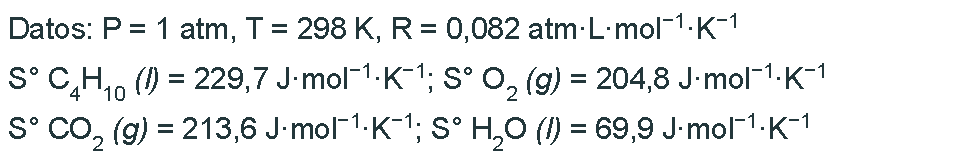
\includegraphics[width=0.75\linewidth]{FigurasSVG/UD4_Termodinamica/pdf/UD4_E01_datos_pau_2023_julio.pdf}
\begin{solu}

\end{solu}
\end{exerciseEVAU}

\begin{exerciseEVAU}
    Dada ls ecuación de la reacción de combustión del etanol:
    \begin{equation*}
        \ch{C2H6 \lqd{} + O2 \gas{} -> CO2 \gas{} + H2O \lqd{}}
    \end{equation*}
    \begin{enumerate}[label=\letraminuscula]
        \item Ajuste la ecuación y calcula la entalpía de combustión del etanol.
        \item Calcule la variación de entropía de esta reacción.
        \item Determine si el proceso será espontáneo a 25 ºC
    \end{enumerate}
    \textbf{Datos:}
    % [FIGURA ORIGINAL] \includegraphics[scale=0.5]{images/imagesUD4Termidonamica/UD4_Problemas/pau_2023_datos}
    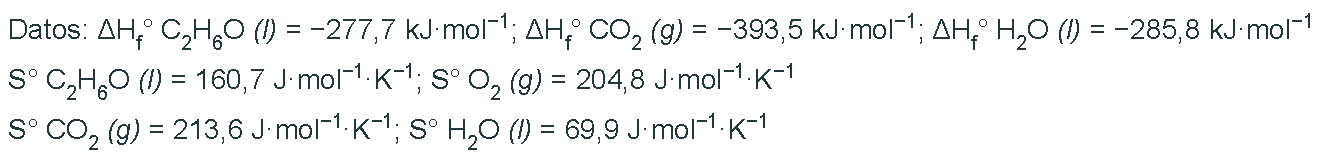
\includegraphics[width=0.95\linewidth]{FigurasSVG/UD4_Termodinamica/pdf/UD4_E02_datos_pau_2023.pdf}
\begin{solu}

\end{solu}
\end{exerciseEVAU}

\begin{exerciseEVAU}
    El aluminio es un agente eficiente para la reducción de óxidos metálicos. Un ejemplo de ello es la reducción
    del óxido de hierro (III), \ch{Fe2O3}, a hierro metálico según la siguiente reacción.
    \begin{centeredequation}
        \ch{Fe2O3 \sld{} + 2 Al \sld{} -> Al2O3 \sld{} + 2 Fe \sld{}}
    \end{centeredequation}
    \begin{enumerate}[label=\letraminuscula]
        \item Calcule la variación de entalpía estándar de esta reacción.
        \item Calcule el calor desprendido en la reducción de 100 g de \ch{Fe2O3}.
        \item Calcule la variación de energía libre de Gibbs a 298 K. ¿Es espontánea la reacción a esa
        temperatura? Justifique la respuesta.
    \end{enumerate}
    \textbf{Datos:} \(  \Delta H^{0}_{f}  [\ch{Fe2O3 \sld{}}] = \qty{- 821,37}{\kjpmol}; \Delta H^{0}_{f}  [\ch{Al2O3 \sld{}}] = \qty{- 1668,24}{\kjpmol};
%    S^0 [\ch{Fe2O3 \sld{}}]= \qty{90}{\jpmol}; S^{0} [\ch{Al2O3 \sld{}}] = \qty{51}{\jpmol}; S^0 [\ch{Al \sld{}}]= \qty{28,3}{\jpmol}; S^{0} [\ch{Fe \sld{}}]= \qty{27,2}{\jpmol}
    \)

    \begin{solu}

        \textbf{a) Entalpía estándar de la reacción}

        La reacción ya está ajustada:
        \begin{equation*}
            \ch{Fe2O3 \sld{} + 2 Al \sld{} -> Al2O3 \sld{} + 2 Fe \sld{}}
        \end{equation*}

        Aplicando la ley de Hess, la entalpía de reacción se calcula como la diferencia entre las entalpías de formación de productos y reactivos (recordando que la entalpía de formación de un elemento en su forma más estable, como \ch{Al \sld{}} y \ch{Fe \sld{}}, es cero):

        \begin{equation*}
            \Delta H^0_{rxn} = \left[ \Delta H^0_f (\ch{Al2O3}) + 2\, \Delta H^0_f (\ch{Fe}) \right] - \left[ \Delta H^0_f (\ch{Fe2O3}) + 2\, \Delta H^0_f (\ch{Al}) \right]
        \end{equation*}

        \begin{equation*}
            \Delta H^0_{rxn} = \left[ -1668,24 + 0 \right] - \left[ -821,37 + 0 \right] = \energia[kj]{-846.87}
        \end{equation*}

        Como \(\Delta H^0 < 0\), la reacción es exotérmica.

        \textbf{b) Calor desprendido en la reducción de 100 g de \ch{Fe2O3}}

        Calculamos la masa molar del \ch{Fe2O3} (M(Fe) = 55,85 u, M(O) = 16 u):

        \begin{equation*}
            M(\ch{Fe2O3}) = 2(55,85) + 3(16) = \SI{159.7}{\gram\per\mole}
        \end{equation*}

        Los moles de \ch{Fe2O3} que reaccionan son:

        \begin{equation*}
            n(\ch{Fe2O3}) = \dfrac{100 \ \si{\gram}}{159,7 \ \si{\gram\per\mole}} = 0,626 \ \text{mol}
        \end{equation*}

        Como la reacción libera \(846,87\) kJ por cada mol de \ch{Fe2O3} que reacciona:

        \begin{equation*}
            q = 0,626 \ \text{mol} \times \energia[kjmol]{846.87} = \energia[kj]{530.3}
        \end{equation*}

        Se desprenden, por tanto, \energia[kj]{530.3} en la reducción de 100 g de \ch{Fe2O3}.

        \textbf{c) Energía de Gibbs a 298 K y espontaneidad}

        En esta reacción todas las especies (reactivos y productos) son sólidos, por lo que no hay una variación significativa en el grado de desorden del sistema: el número de partículas gaseosas no cambia (de hecho no hay ninguna especie gaseosa), así que \(\Delta S^0 \approx 0\).

        En estas condiciones:

        \begin{equation*}
            \Delta G^0 = \Delta H^0 - T \Delta S^0 \approx \Delta H^0 = \energia[kj]{-846.87}
        \end{equation*}

        Como \(\Delta G^0 < 0\), la reacción \textbf{es espontánea} a 298 K. Esto es coherente con el hecho de que el aluminio es, en la práctica, un potente reductor de óxidos metálicos (proceso conocido como aluminotermia).

    \end{solu}
\end{exerciseEVAU}

\begin{exerciseEVAU}
    Existen bacterias que degradan la glucosa (\ch{C6H12O6}) mediante un proceso denominado fermentación
    alcohólica, en el cual se produce etanol (\ch{CH3-CH2OH}) y dióxido de carbono (\ch{CO2}) según la siguiente
    reacción:
    \begin{centeredequation}
        \ch{C6H12O6 \gas{} -> 2 CH3-CH3OH \lqd{} + 2 CO2 \gas{}}
    \end{centeredequation}
    \begin{enumerate}[label=\letraminuscula]
    \item Utilizando la Ley de Hess, determine la energía intercambiada en la fermentación de un mol
    de glucosa.
    \item Indique si dicha reacción es endotérmica o exotérmica, justificando la respuesta.
    \item Calcule la cantidad de calor que se produce en la fermentación de 1 Kg de glucosa.
    \end{enumerate}
    \textbf{Datos:}  Las entalpías de combustión de la glucosa y del etanol son –2815 kJ/mol y –1372 kJ/mol,
    respectivamente. Masas atómicas: (C) = 12 u; (O) = 16 u; (H) = 1 u.

    \begin{solu}

        \textbf{a) Energía intercambiada en la fermentación de un mol de glucosa (Ley de Hess)}

        La reacción de fermentación es:

        \begin{equation*}
            \ch{C6H12O6 \sld{} -> 2 CH3CH2OH \lqd{} + 2 CO2 \gas{}}
        \end{equation*}

        Para aplicar la ley de Hess necesitamos las reacciones de combustión de la glucosa y del etanol:

        \begin{align*}
            \text{(1)} \quad & \ch{C6H12O6 \sld{} + 6 O2 \gas{} -> 6 CO2 \gas{} + 6 H2O \lqd{}} \quad \Delta H_1 = \energia[kjmol]{-2815} \\
            \text{(2)} \quad & \ch{CH3CH2OH \lqd{} + 3 O2 \gas{} -> 2 CO2 \gas{} + 3 H2O \lqd{}} \quad \Delta H_2 = \energia[kjmol]{-1372}
        \end{align*}

        Para obtener la reacción de fermentación a partir de estas dos, mantenemos la reacción (1) y restamos dos veces la reacción (2) (es decir, invertimos dos veces la combustión del etanol y la sumamos a la de la glucosa):

        \begin{equation*}
            \Delta H_{ferm} = \Delta H_1 - 2 \Delta H_2 = -2815 - 2(-1372) = -2815 + 2744 = \energia[kjmol]{-71}
        \end{equation*}

        Por tanto, en la fermentación de 1 mol de glucosa se desprenden \energia[kjmol]{71}.

        \textbf{b) Carácter endotérmico o exotérmico}

        Como \(\Delta H_{ferm} = \energia[kjmol]{-71} < 0\), el proceso desprende calor al entorno, por lo que la reacción es \textbf{exotérmica}.

        \textbf{c) Calor producido en la fermentación de 1 kg de glucosa}

        La masa molar de la glucosa (\ch{C6H12O6}) es:

        \begin{equation*}
            M(\ch{C6H12O6}) = 6(12) + 12(1) + 6(16) = \SI{180}{\gram\per\mole}
        \end{equation*}

        Los moles contenidos en 1 kg (1000 g) de glucosa son:

        \begin{equation*}
            n = \dfrac{1000 \ \si{\gram}}{180 \ \si{\gram\per\mole}} = 5,56 \ \text{mol}
        \end{equation*}

        El calor desprendido será:

        \begin{equation*}
            q = 5,56 \ \text{mol} \times \energia[kjmol]{71} = \energia[kj]{394.4}
        \end{equation*}

        Se desprenden, por tanto, aproximadamente \energia[kj]{394.4} en la fermentación de 1 kg de glucosa.

    \end{solu}
\end{exerciseEVAU}


\begin{exerciseEVAU}
    \textbf{2024}.
    \begin{reaction*}
        C2H6O \lqd{} + O2 \gas{} -> CO2 \gas{} + H2O \lqd{}
    \end{reaction*}

    \begin{enumerate}[label=\letraminuscula]
         \item Ajuste la ecuación y calcule la entalpía de combustión del etanol.
         \item Calcule la variación de entropía de esta reacción.
         \item Determine si este proceso será espontáneo a \SI{25}{\celsius}.
    \end{enumerate}

    \datos{}: \( \Delta H^0_f\  \ch{C2H6O \lqd{}} = \SI{-277.7}{\kjpmol}  \); \( \Delta H^0_f\ \ch{CO2 \gas{}} = \SI{-393.5}{\kjpmol} \); \( \Delta H^0_f\ \ch{H2O \lqd{}} = \SI{-285.8}{\kjpmol} \); \( \Delta S^0_f\ \ch{C2H6O \lqd{}} = \SI{160.7}{\jpmolpk} \); \( \Delta S^0_f\ \ch{O2 \gas{}} = \SI{204.8}{\jpmolpk} \); \( \Delta S^0_f\ \ch{CO2 \gas{}} = \SI{213.6}{\jpmolpk} \); \( \Delta S^0_f\ \ch{H2O \lqd{}} = \SI{69.9}{\jpmolpk} \)
    \begin{solu}

        \textbf{a) Ajuste de la ecuación y entalpía de combustión del etanol}

        La ecuación ajustada de la combustión del etanol es:

        \begin{equation*}
            \ch{C2H6O \lqd{} + 3 O2 \gas{} -> 2 CO2 \gas{} + 3 H2O \lqd{}}
        \end{equation*}

        Aplicando la ley de Hess:

        \begin{equation*}
            \Delta H^0_{rxn} = \left[ 2\, \Delta H^0_f (\ch{CO2}) + 3\, \Delta H^0_f (\ch{H2O}) \right] - \left[ \Delta H^0_f (\ch{C2H6O}) + 3\, \Delta H^0_f (\ch{O2}) \right]
        \end{equation*}

        \begin{equation*}
            \Delta H^0_{rxn} = \left[ 2(-393,5) + 3(-285,8) \right] - \left[ -277,7 + 0 \right] = -1644,4 + 277,7 = \energia[kjmol]{-1366.7}
        \end{equation*}

        \textbf{b) Variación de entropía de la reacción}

        \begin{equation*}
            \Delta S^0_{rxn} = \left[ 2\, S^0 (\ch{CO2}) + 3\, S^0 (\ch{H2O}) \right] - \left[ S^0 (\ch{C2H6O}) + 3\, S^0 (\ch{O2}) \right]
        \end{equation*}

        \begin{equation*}
            \Delta S^0_{rxn} = \left[ 2(213,6) + 3(69,9) \right] - \left[ 160,7 + 3(204,8) \right] = 636,9 - 775,1 = \SI{-138.2}{\jpmolpk}
        \end{equation*}

        El signo negativo es coherente: se pasa de 1 mol de líquido más 3 mol de gas (4 mol de gas) a 2 mol de gas más 3 mol de líquido (2 mol de gas), disminuyendo el número de moles gaseosos y, por tanto, el desorden del sistema.

        \textbf{c) Espontaneidad del proceso a 25 ºC}

        A \(T = \SI{298}{\kelvin}\):

        \begin{equation*}
            \Delta G^0 = \Delta H^0 - T \Delta S^0 = -1366,7 - 298 \cdot (-0,1382) = -1366,7 + 41,2 = \energia[kj]{-1325.5}
        \end{equation*}

        Como \(\Delta G^0 < 0\), el proceso \textbf{es espontáneo} a \SI{25}{\celsius}.

    \end{solu}
\end{exerciseEVAU}

\begin{exerciseEVAU}
    \textbf{2020}. Para la reacción química \ch{A + B -> 2 C}, se conoce el valor absoluto de la variación de entalpía, \(|\Delta H | = \SI{68}{\kilo\joule}\), y la variación de entropía, \(\Delta S = \SI{2}{\joule\per\kelvin}\).
    Coméntese razonadamente si la reacción es espontánea a \temperatura[c]{25}.

    \begin{solu}

        Como solo se nos da el valor absoluto de \(\Delta H\), debemos estudiar los dos casos posibles.

        A \(T = \SI{298}{\kelvin}\), el término entrópico vale:

        \begin{equation*}
            T \Delta S = 298 \ \si{\kelvin} \times \SI{2}{\joule\per\kelvin} = \SI{596}{\joule} = \SI{0.596}{\kilo\joule}
        \end{equation*}

        Este valor es muy pequeño frente a los \(\SI{68}{\kilo\joule}\) de \(|\Delta H|\), por lo que el signo de \(\Delta G\) va a estar determinado, prácticamente en su totalidad, por el signo de \(\Delta H\).

        \textbf{Caso a) Si la reacción es exotérmica} (\(\Delta H = \energia[kj]{-68}\)):

        \begin{equation*}
            \Delta G = \Delta H - T \Delta S = -68 - 0,596 = \energia[kj]{-68.6}
        \end{equation*}

        Como \(\Delta G < 0\), la reacción \textbf{sería espontánea} a \SI{25}{\celsius}.

        \textbf{Caso b) Si la reacción es endotérmica} (\(\Delta H = \energia[kj]{68}\)):

        \begin{equation*}
            \Delta G = \Delta H - T \Delta S = 68 - 0,596 = \energia[kj]{67.4}
        \end{equation*}

        Como \(\Delta G > 0\), la reacción \textbf{no sería espontánea} a \SI{25}{\celsius}.

        En conclusión, dado que la contribución entrópica (\(T \Delta S\)) es muy pequeña, la espontaneidad de esta reacción a \SI{25}{\celsius} depende casi exclusivamente de si el proceso es exotérmico (espontáneo) o endotérmico (no espontáneo), sin que la temperatura ambiente sea capaz de invertir dicha tendencia.

    \end{solu}
\end{exerciseEVAU}

\begin{exerciseEVAU}
    \textbf{2017} En los siguientes sistemas en equilibrio,
    \begin{enumerate}[label=\letraminuscula]
     \item \(\ch{A <=> 2 B}\quad \Delta H^0 = \energia[kjmol]{20.0}\)
     \item \(\ch{A + B <=>  B}\quad \Delta H^0 = \energia[kjmol]{-5.4}\)
     \item \(\ch{A <=>  B}\quad \Delta H^0 = \energia[kjmol]{0.0}\)
    \end{enumerate}
    predice razonadamente el cambio que se produciría en cada uno de ellos al aumentar la temperatura.
    \begin{solu}

        Un aumento de la temperatura desplaza siempre el equilibrio en el sentido de la reacción \textbf{endotérmica}, ya que de esa forma el sistema absorbe parte de la energía suministrada, contrarrestando la perturbación (principio de Le Chatelier).

        \textbf{a)} \(\ch{A <=> 2 B}\), con \(\Delta H^0 = \energia[kjmol]{20.0} > 0\) (reacción directa endotérmica).

        Al aumentar la temperatura, el equilibrio se desplaza hacia la \textbf{derecha}, es decir, hacia la formación de \ch{B}, aumentando su concentración y disminuyendo la de \ch{A}.

        \textbf{b)} \(\ch{A + B <=> B}\), con \(\Delta H^0 = \energia[kjmol]{-5.4} < 0\) (reacción directa exotérmica).

        Al aumentar la temperatura, el equilibrio se desplaza hacia la \textbf{izquierda} (sentido endotérmico, el inverso), favoreciendo la formación de \ch{A}, es decir, disminuye la conversión de \ch{A} en el sentido directo.

        \textbf{c)} \(\ch{A <=> B}\), con \(\Delta H^0 = \energia[kjmol]{0.0}\) (la reacción no absorbe ni desprende calor).

        Al no haber intercambio de calor asociado a la reacción, un aumento de la temperatura \textbf{no modifica la posición del equilibrio}: la constante de equilibrio \(K\) prácticamente no varía con la temperatura (según la ecuación de Van't Hoff, si \(\Delta H^0 = 0\), \(K\) es independiente de \(T\)).

    \end{solu}
\end{exerciseEVAU}


\begin{exerciseEVAU}
    \textbf{2016} La hidracina, \ch{N2H4}, es un combustible líquido que ha sido utilizado para la propulsión de misiles y cohetes espaciales. La reacción de combustión de la hidracina con oxígeno gas da como resultado nitrógeno
    molecular y agua gas.
    \begin{enumerate}[label=\letraminuscula]
    \item  Escribe la ecuación ajustada de la reacción anterior así como las de formación de la hidracina
    líquida y el agua gas.
    \item Calcula la entalpía de la reacción de combustión de la hidracina sabiendo que al reaccionar
    100 g de esta sustancia se desprenden 1672 kJ.
    \item Calcula la entalpía estándar de formación de la hidracina líquida.
    \end{enumerate}
    \datos{}: \(\Delta H^0_f (\ch{H2O \gas{}}) = \energia[kjmol]{-241.8}\). Masas atómicas: N = 14, H = 1.
    \begin{solu}

        \textbf{a) Ecuaciones ajustadas}

        Combustión de la hidracina (da nitrógeno molecular y agua gas):

        \begin{equation*}
            \ch{N2H4 \lqd{} + O2 \gas{} -> N2 \gas{} + 2 H2O \gas{}}
        \end{equation*}

        Formación de la hidracina líquida:

        \begin{equation*}
            \ch{N2 \gas{} + 2 H2 \gas{} -> N2H4 \lqd{}}
        \end{equation*}

        Formación del agua gas:

        \begin{equation*}
            \ch{H2 \gas{} + 1/2 O2 \gas{} -> H2O \gas{}}
        \end{equation*}

        \textbf{b) Entalpía de combustión de la hidracina}

        La masa molar de la hidracina es:

        \begin{equation*}
            M(\ch{N2H4}) = 2(14) + 4(1) = \SI{32}{\gram\per\mole}
        \end{equation*}

        Los moles que reaccionan al quemar 100 g de hidracina son:

        \begin{equation*}
            n = \dfrac{100 \ \si{\gram}}{32 \ \si{\gram\per\mole}} = 3,125 \ \text{mol}
        \end{equation*}

        Como al reaccionar esos 3,125 mol se desprenden 1672 kJ, la entalpía molar de combustión es:

        \begin{equation*}
            \Delta H^0_{comb} = \dfrac{-1672 \ \si{\kilo\joule}}{3,125 \ \text{mol}} = \energia[kjmol]{-535.0}
        \end{equation*}

        \textbf{c) Entalpía estándar de formación de la hidracina líquida}

        Aplicando la ley de Hess a la reacción de combustión:

        \begin{equation*}
            \Delta H^0_{comb} = \left[ \Delta H^0_f (\ch{N2}) + 2\, \Delta H^0_f (\ch{H2O \gas{}}) \right] - \left[ \Delta H^0_f (\ch{N2H4}) + \Delta H^0_f (\ch{O2}) \right]
        \end{equation*}

        Como \(\Delta H^0_f (\ch{N2}) = \Delta H^0_f (\ch{O2}) = 0\) (elementos en su estado estándar):

        \begin{equation*}
            -535,0 = \left[ 0 + 2(-241,8) \right] - \Delta H^0_f (\ch{N2H4}) = -483,6 - \Delta H^0_f (\ch{N2H4})
        \end{equation*}

        \begin{equation*}
            \Delta H^0_f (\ch{N2H4}) = -483,6 + 535,0 = \energia[kjmol]{51.4}
        \end{equation*}

        La entalpía de formación de la hidracina líquida es positiva (\energia[kjmol]{51.4}), lo que indica que se trata de un compuesto endotérmico, con un elevado contenido energético; precisamente por ello es adecuada como combustible de alta energía para cohetes.

    \end{solu}
\end{exerciseEVAU}

\begin{exerciseEVAU}
    \textbf{2015} Sabiendo que las entalpías estándar de combustión del eteno y del etano son \energia[kjmol]{-1386.1} y \energia[kjmol]{-1539.9} kJ/mol respectivamente, y que la entalpía estándar de formación del agua es \energia[kjmol]{-285,8}:
    \begin{enumerate}[label=\letraminuscula]
    \item Escribe las reacciones correspondientes a los procesos citados y a la hidrogenación del eteno para dar etano.
    \item Calcula la entalpía estándar de hidrogenación del eteno.
    \item  Calcula la energía que se desprenderá al obtener 4,89 L de \ch{CO2},medidos a 760 mm de Hg de presión y \temperatura[c]{25} de temperatura, mediante la combustión del etano.
    \end{enumerate}
    \datos{}: \(R = \ctegases\)
    \begin{solu}

        \textbf{a) Ecuaciones de los procesos}

        Combustión del eteno:

        \begin{equation*}
            \ch{C2H4 \gas{} + 3 O2 \gas{} -> 2 CO2 \gas{} + 2 H2O \lqd{}} \quad \Delta H^0_1 = \energia[kjmol]{-1386.1}
        \end{equation*}

        Combustión del etano:

        \begin{equation*}
            \ch{C2H6 \gas{} + 7/2 O2 \gas{} -> 2 CO2 \gas{} + 3 H2O \lqd{}} \quad \Delta H^0_2 = \energia[kjmol]{-1539.9}
        \end{equation*}

        Hidrogenación del eteno para dar etano:

        \begin{equation*}
            \ch{C2H4 \gas{} + H2 \gas{} -> C2H6 \gas{}}
        \end{equation*}

        \textbf{b) Entalpía estándar de hidrogenación del eteno}

        Para aplicar la ley de Hess necesitamos también la reacción de combustión (formación de agua) del hidrógeno:

        \begin{equation*}
            \ch{H2 \gas{} + 1/2 O2 \gas{} -> H2O \lqd{}} \quad \Delta H^0_3 = \Delta H^0_f (\ch{H2O}) = \energia[kjmol]{-285.8}
        \end{equation*}

        La reacción de hidrogenación se obtiene sumando la combustión del eteno y la del hidrógeno, y restando la combustión del etano (\(\Delta H_{hidrog} = \Delta H^0_1 + \Delta H^0_3 - \Delta H^0_2\)):

        \begin{equation*}
            \Delta H^0_{hidrog} = -1386,1 + (-285,8) - (-1539,9) = -1386,1 - 285,8 + 1539,9 = \energia[kjmol]{-132.0}
        \end{equation*}

        \textbf{c) Energía desprendida al obtener 4,89 L de \ch{CO2} en la combustión del etano}

        Calculamos los moles de \ch{CO2} mediante la ecuación de los gases ideales, con \(P = \SI{760}{\mmhg} = \SI{1}{\atmospher}\) y \(T = \temperatura[k]{298}\):

        \begin{equation*}
            n(\ch{CO2}) = \dfrac{PV}{RT} = \dfrac{1 \cdot 4,89}{0,082 \cdot 298} = 0,200 \ \text{mol}
        \end{equation*}

        En la combustión del etano se producen 2 mol de \ch{CO2} por cada mol de \ch{C2H6} quemado, liberando \(1539,9\) kJ. Por tanto, la energía liberada por mol de \ch{CO2} formado es:

        \begin{equation*}
            \dfrac{\Delta H^0_2}{2} = \dfrac{-1539,9}{2} = \energia[kjmol]{-770.0}
        \end{equation*}

        La energía desprendida al formarse 0,200 mol de \ch{CO2} es:

        \begin{equation*}
            q = 0,200 \ \text{mol} \times \energia[kjmol]{770.0} = \energia[kj]{154.0}
        \end{equation*}

    \end{solu}
\end{exerciseEVAU}

\begin{exerciseEVAU}
    \textbf{2015} Las entalpías estándar de combustión del benceno (\ch{C6H6}) y del carbono son \energia[kjmol]{-3267} y \energia[kjmol]{-393,7}, respectivamente, y la entalpía estándar de formación del agua líquida es \energia[kjmol]{-285,8}.
    \begin{enumerate}[label=\letraminuscula]
    \item Escribe las reacciones correspondientes a los procesos citados y al de formación del benceno.
    \item Calcula la entalpía estándar de formación del benceno.
    \item Calcula la energía que se desprenderá o absorberá en la combustión de 500 g de benceno en condiciones estándar.
    \end{enumerate}
    \datos{}: Masas atómicas: C = 12; H = 1.

    \begin{solu}

        \textbf{a) Ecuaciones de los procesos}

        Combustión del benceno:

        \begin{equation*}
            \ch{C6H6 \lqd{} + 15/2 O2 \gas{} -> 6 CO2 \gas{} + 3 H2O \lqd{}} \quad \Delta H^0_1 = \energia[kjmol]{-3267}
        \end{equation*}

        Combustión del carbono (formación del \ch{CO2}):

        \begin{equation*}
            \ch{C \sld{} + O2 \gas{} -> CO2 \gas{}} \quad \Delta H^0_2 = \energia[kjmol]{-393.7}
        \end{equation*}

        Formación del agua líquida:

        \begin{equation*}
            \ch{H2 \gas{} + 1/2 O2 \gas{} -> H2O \lqd{}} \quad \Delta H^0_3 = \energia[kjmol]{-285.8}
        \end{equation*}

        Formación del benceno:

        \begin{equation*}
            \ch{6 C \sld{} + 3 H2 \gas{} -> C6H6 \lqd{}} \quad \Delta H^0_f = \ ?
        \end{equation*}

        \textbf{b) Entalpía estándar de formación del benceno}

        Por la ley de Hess, la entalpía de combustión se relaciona con las entalpías de formación de productos y reactivos:

        \begin{equation*}
            \Delta H^0_1 = \left[ 6\, \Delta H^0_2 + 3\, \Delta H^0_3 \right] - \Delta H^0_f (\ch{C6H6})
        \end{equation*}

        \begin{equation*}
            -3267 = \left[ 6(-393,7) + 3(-285,8) \right] - \Delta H^0_f (\ch{C6H6}) = -3219,6 - \Delta H^0_f (\ch{C6H6})
        \end{equation*}

        \begin{equation*}
            \Delta H^0_f (\ch{C6H6}) = -3219,6 + 3267 = \energia[kjmol]{47.4}
        \end{equation*}

        El valor positivo indica que el benceno es un compuesto endotérmico (su formación a partir de los elementos absorbe energía).

        \textbf{c) Energía en la combustión de 500 g de benceno}

        La masa molar del benceno es:

        \begin{equation*}
            M(\ch{C6H6}) = 6(12) + 6(1) = \SI{78}{\gram\per\mole}
        \end{equation*}

        \begin{equation*}
            n = \dfrac{500 \ \si{\gram}}{78 \ \si{\gram\per\mole}} = 6,41 \ \text{mol}
        \end{equation*}

        \begin{equation*}
            q = 6,41 \ \text{mol} \times \energia[kjmol]{3267} = \energia[kj]{20942}
        \end{equation*}

        Al ser la combustión un proceso exotérmico, se \textbf{desprenden} aproximadamente \energia[kj]{20942} al quemar 500 g de benceno.

    \end{solu}
\end{exerciseEVAU}

\begin{exerciseEVAU}
    \textbf{2014} Sabiendo que las entalpías estándar de formación del \ch{CO2 \gas{}} y del \ch{H2O \lqd{}}  son \energia[kjmol]{-393,3} y \energia[kjmol]{-285,8}, respectivamente, y que el calor de combustión del ácido acético líquido (ácido etanoico), a \temperatura[c]{25}, es \energia[kjmol]{-874}:
    \begin{enumerate}[label=\letraminuscula]
    \item Escribe las reacciones correspondientes a los procesos citados y la de formación del ácido acético líquido.
    \item Calcula la entalpía estándar de formación del ácido acético líquido.
    \item Calcula la energía que se desprenderá al obtener 25 litros de \ch{CO2}, medidos a 740 mm de Hg de presión y \temperatura[c]{25}, mediante la combustión del ácido acético líquido.
    \end{enumerate}
    \datos{}: \(R = \ctegases\)

    \begin{solu}

        \textbf{a) Ecuaciones de los procesos}

        Combustión del ácido acético líquido:

        \begin{equation*}
            \ch{CH3COOH \lqd{} + 2 O2 \gas{} -> 2 CO2 \gas{} + 2 H2O \lqd{}} \quad \Delta H^0_1 = \energia[kjmol]{-874}
        \end{equation*}

        Formación del \ch{CO2}:

        \begin{equation*}
            \ch{C \sld{} + O2 \gas{} -> CO2 \gas{}} \quad \Delta H^0_2 = \energia[kjmol]{-393.3}
        \end{equation*}

        Formación del agua líquida:

        \begin{equation*}
            \ch{H2 \gas{} + 1/2 O2 \gas{} -> H2O \lqd{}} \quad \Delta H^0_3 = \energia[kjmol]{-285.8}
        \end{equation*}

        Formación del ácido acético líquido:

        \begin{equation*}
            \ch{2 C \sld{} + 2 H2 \gas{} + O2 \gas{} -> CH3COOH \lqd{}} \quad \Delta H^0_f = \ ?
        \end{equation*}

        \textbf{b) Entalpía estándar de formación del ácido acético líquido}

        \begin{equation*}
            \Delta H^0_1 = \left[ 2\, \Delta H^0_2 + 2\, \Delta H^0_3 \right] - \Delta H^0_f (\ch{CH3COOH})
        \end{equation*}

        \begin{equation*}
            -874 = \left[ 2(-393,3) + 2(-285,8) \right] - \Delta H^0_f (\ch{CH3COOH}) = -1358,2 - \Delta H^0_f (\ch{CH3COOH})
        \end{equation*}

        \begin{equation*}
            \Delta H^0_f (\ch{CH3COOH}) = -1358,2 + 874 = \energia[kjmol]{-484.2}
        \end{equation*}

        \textbf{c) Energía desprendida al obtener 25 L de \ch{CO2}}

        Con \(P = \dfrac{740}{760} = 0,974 \ \si{\atmospher}\) y \(T = \temperatura[k]{298}\), calculamos los moles de \ch{CO2} mediante la ecuación de los gases ideales:

        \begin{equation*}
            n(\ch{CO2}) = \dfrac{PV}{RT} = \dfrac{0,974 \times 25}{0,082 \times 298} = 0,996 \ \text{mol}
        \end{equation*}

        Como en la combustión se forman 2 mol de \ch{CO2} por cada mol de ácido, liberando \(874\) kJ, la energía por mol de \ch{CO2} es:

        \begin{equation*}
            \dfrac{\Delta H^0_1}{2} = \dfrac{-874}{2} = \energia[kjmol]{-437}
        \end{equation*}

        \begin{equation*}
            q = 0,996 \ \text{mol} \times \energia[kjmol]{437} = \energia[kj]{435.3}
        \end{equation*}

    \end{solu}
\end{exerciseEVAU}

\begin{exerciseEVAU}
    \textbf{2014} La entalpía estándar de combustión de la propanona (\ch{CH3-CO-CH3}) es \energia[kjmol]{-1787,2}. Las entalpías estándar de formación del dióxido de carbono gaseoso y del agua líquida son \energia[kjmol]{-393,5} y \energia[kjmol]{-285,8}, respectivamente.
    \begin{enumerate}[label=\letraminuscula]
    \item Escribe las reacciones anteriores y la de formación de la propanona.
    \item Calcula la entalpía estándar de formación de la propanona.
    \item Calcula los gramos de propanona que deben quemarse para generar \energia[kj]{3500} de energía calorífica.
    \end{enumerate}
    \datos{}: Masas atómicas: C = 12; H = 1; O = 16.

    \begin{solu}

        \textbf{a) Ecuaciones de los procesos}

        Combustión de la propanona:

        \begin{equation*}
            \ch{CH3-CO-CH3 \lqd{} + 4 O2 \gas{} -> 3 CO2 \gas{} + 3 H2O \lqd{}} \quad \Delta H^0_1 = \energia[kjmol]{-1787.2}
        \end{equation*}

        Formación del \ch{CO2}:

        \begin{equation*}
            \ch{C \sld{} + O2 \gas{} -> CO2 \gas{}} \quad \Delta H^0_2 = \energia[kjmol]{-393.5}
        \end{equation*}

        Formación del agua líquida:

        \begin{equation*}
            \ch{H2 \gas{} + 1/2 O2 \gas{} -> H2O \lqd{}} \quad \Delta H^0_3 = \energia[kjmol]{-285.8}
        \end{equation*}

        Formación de la propanona:

        \begin{equation*}
            \ch{3 C \sld{} + 3 H2 \gas{} + 1/2 O2 \gas{} -> CH3-CO-CH3 \lqd{}} \quad \Delta H^0_f = \ ?
        \end{equation*}

        \textbf{b) Entalpía estándar de formación de la propanona}

        \begin{equation*}
            \Delta H^0_1 = \left[ 3\, \Delta H^0_2 + 3\, \Delta H^0_3 \right] - \Delta H^0_f (\ch{propanona})
        \end{equation*}

        \begin{equation*}
            -1787,2 = \left[ 3(-393,5) + 3(-285,8) \right] - \Delta H^0_f (\ch{propanona}) = -2037,9 - \Delta H^0_f (\ch{propanona})
        \end{equation*}

        \begin{equation*}
            \Delta H^0_f (\ch{propanona}) = -2037,9 + 1787,2 = \energia[kjmol]{-250.7}
        \end{equation*}

        \textbf{c) Gramos de propanona para generar 3500 kJ}

        La masa molar de la propanona (\ch{C3H6O}) es:

        \begin{equation*}
            M(\ch{C3H6O}) = 3(12) + 6(1) + 16 = \SI{58}{\gram\per\mole}
        \end{equation*}

        Como cada mol de propanona quemado libera 1787,2 kJ, los moles necesarios para generar 3500 kJ son:

        \begin{equation*}
            n = \dfrac{3500 \ \si{\kilo\joule}}{1787,2 \ \si{\kjpmol}} = 1,958 \ \text{mol}
        \end{equation*}

        \begin{equation*}
            m = 1,958 \ \text{mol} \times 58 \ \si{\gram\per\mole} = \SI{113.6}{\gram}
        \end{equation*}

    \end{solu}
\end{exerciseEVAU}

\begin{exerciseEVAU}
    \textbf{2014} Justifica el signo de \(\Delta S\) y la espontaneidad de la reacción de formación del amoniaco gaseoso:
    \begin{equation*}
        \ch{N2 \gas{} + 3 H2 \gas{} -> 2 NH3 \gas{}} \quad \Delta H <0
    \end{equation*}

    \begin{solu}

        \textbf{Signo de \(\Delta S\)}

        En esta reacción, todas las especies son gaseosas. El número de moles de gas pasa de \(1 + 3 = 4\) mol en los reactivos a \(2\) mol en los productos, es decir, \(\Delta n_{gas} = 2 - 4 = -2 < 0\).

        Al disminuir el número de moles gaseosos, el sistema pasa a un estado más ordenado (menor número de partículas libres en fase gas), por lo que \(\boldsymbol{\Delta S < 0}\).

        \textbf{Espontaneidad}

        La espontaneidad viene determinada por el signo de \(\Delta G = \Delta H - T \Delta S\). Aquí \(\Delta H < 0\) (dato del enunciado) y \(\Delta S < 0\) (deducido arriba), por lo que el término \(-T\Delta S\) es siempre positivo y crece con la temperatura.

        \begin{itemize}
            \item A \textbf{bajas temperaturas}, el término \(\Delta H\) (negativo) predomina sobre \(-T\Delta S\) (positivo, pero pequeño), de modo que \(\Delta G < 0\): la reacción es \textbf{espontánea}.
            \item A \textbf{temperaturas suficientemente altas}, el término \(-T\Delta S\) puede superar en magnitud a \(\Delta H\), haciendo que \(\Delta G > 0\): la reacción deja de ser espontánea.
        \end{itemize}

        Por tanto, la síntesis de amoniaco es termodinámicamente más favorable a bajas temperaturas, lo cual concuerda con la necesidad de emplear un catalizador en el proceso Haber-Bosch para conseguir una velocidad de reacción aceptable sin tener que recurrir a temperaturas muy elevadas (que perjudicarían el rendimiento termodinámico).

    \end{solu}
\end{exerciseEVAU}

\begin{exerciseEVAU}
    \textbf{2013} A partir de los datos de la tabla adjunta:

    \begin{figure}[H]
        \centering
        % [FIGURA ORIGINAL] \includegraphics[scale=0.6]{images/imagesUD4Termidonamica/UD4_Problemas/EvAU_2013.png}
        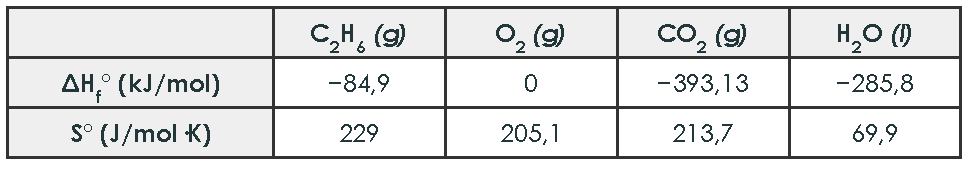
\includegraphics[width=0.75\linewidth]{FigurasSVG/UD4_Termodinamica/pdf/UD4_E03_tabla_EvAU_2013.pdf}
        %\caption{}
        %\label{fig:}
    \end{figure}

    \begin{enumerate}[label=\letraminuscula]
    \item Calcula la variación de entalpía y de entropía, en condiciones estándar, para la combustión del etano.
    \item Calcula \(\Delta G^0\) para la reacción anterior e indica si esta es espontánea a 298 K y 1 atm
    \end{enumerate}
    \begin{solu}

        La tabla adjunta proporciona los siguientes datos:

        \begin{center}
        \begin{tabular}{lcccc}
            \toprule
            & \ch{C2H6 \gas{}} & \ch{O2 \gas{}} & \ch{CO2 \gas{}} & \ch{H2O \lqd{}} \\
            \midrule
            \(\Delta H^0_f\) (kJ/mol) & \(-84,9\) & \(0\) & \(-393,13\) & \(-285,8\) \\
            \(S^0\) (J/mol·K) & \(229\) & \(205,1\) & \(213,7\) & \(69,9\) \\
            \bottomrule
        \end{tabular}
        \end{center}

        \textbf{a) Entalpía y entropía de la combustión del etano}

        La reacción de combustión del etano, ajustada, es:

        \begin{equation*}
            \ch{C2H6 \gas{} + 7/2 O2 \gas{} -> 2 CO2 \gas{} + 3 H2O \lqd{}}
        \end{equation*}

        \begin{equation*}
            \Delta H^0 = \left[ 2\, \Delta H^0_f (\ch{CO2}) + 3\, \Delta H^0_f (\ch{H2O}) \right] - \left[ \Delta H^0_f (\ch{C2H6}) + \dfrac{7}{2}\, \Delta H^0_f (\ch{O2}) \right]
        \end{equation*}

        \begin{equation*}
            \Delta H^0 = \left[ 2(-393,13) + 3(-285,8) \right] - \left[ -84,9 + 0 \right] = -1643,66 + 84,9 = \energia[kjmol]{-1558.76}
        \end{equation*}

        \begin{equation*}
            \Delta S^0 = \left[ 2\, S^0 (\ch{CO2}) + 3\, S^0 (\ch{H2O}) \right] - \left[ S^0 (\ch{C2H6}) + \dfrac{7}{2}\, S^0 (\ch{O2}) \right]
        \end{equation*}

        \begin{equation*}
            \Delta S^0 = \left[ 2(213,7) + 3(69,9) \right] - \left[ 229 + 3,5(205,1) \right] = 637,1 - 946,85 = \SI{-309.75}{\jpmolpk}
        \end{equation*}

        \textbf{b) Energía de Gibbs y espontaneidad}

        A \(T = \SI{298}{\kelvin}\):

        \begin{equation*}
            \Delta G^0 = \Delta H^0 - T \Delta S^0 = -1558,76 - 298 \cdot (-0,30975) = -1558,76 + 92,3 = \energia[kj]{-1466.5}
        \end{equation*}

        Como \(\Delta G^0 < 0\), la reacción \textbf{es espontánea} a 298 K y 1 atm.

    \end{solu}
\end{exerciseEVAU}

\begin{exerciseEVAU}
    \textbf{2013} Sabiendo que, a 298 K y 1 atm, las entalpías de combustión del hidrógeno, carbono y eteno son,
    respectivamente, \energia[kjmol]{-285,5},  \energia[kjmol]{-393,13} y \energia[kjmol]{-1421,2}, a) escribe las reacciones correspondientes a las combustiones citadas; b) calcula la entalpía de formación del eteno; c) calcula la energía que se desprenderá, en las condiciones de presión y temperatura anteriores, al obtener 40 L de \ch{CO2} mediante combustión del eteno.
    \datos{}: \(R = \ctegases\)

    \begin{solu}

        \textbf{a) Ecuaciones de combustión}

        Combustión del hidrógeno (formación del agua):

        \begin{equation*}
            \ch{H2 \gas{} + 1/2 O2 \gas{} -> H2O \lqd{}} \quad \Delta H^0_1 = \energia[kjmol]{-285.5}
        \end{equation*}

        Combustión del carbono (formación del \ch{CO2}):

        \begin{equation*}
            \ch{C \sld{} + O2 \gas{} -> CO2 \gas{}} \quad \Delta H^0_2 = \energia[kjmol]{-393.13}
        \end{equation*}

        Combustión del eteno:

        \begin{equation*}
            \ch{C2H4 \gas{} + 3 O2 \gas{} -> 2 CO2 \gas{} + 2 H2O \lqd{}} \quad \Delta H^0_3 = \energia[kjmol]{-1421.2}
        \end{equation*}

        \textbf{b) Entalpía de formación del eteno}

        La reacción de formación del eteno es \(\ch{2 C \sld{} + 2 H2 \gas{} -> C2H4 \gas{}}\). Por la ley de Hess:

        \begin{equation*}
            \Delta H^0_3 = \left[ 2\, \Delta H^0_2 + 2\, \Delta H^0_1 \right] - \Delta H^0_f (\ch{C2H4})
        \end{equation*}

        \begin{equation*}
            -1421,2 = \left[ 2(-393,13) + 2(-285,5) \right] - \Delta H^0_f (\ch{C2H4}) = -1357,26 - \Delta H^0_f (\ch{C2H4})
        \end{equation*}

        \begin{equation*}
            \Delta H^0_f (\ch{C2H4}) = -1357,26 + 1421,2 = \energia[kjmol]{63.9}
        \end{equation*}

        \textbf{c) Energía desprendida al obtener 40 L de \ch{CO2}}

        A \(T = \temperatura[k]{298}\) y \(P = \SI{1}{\atmospher}\):

        \begin{equation*}
            n(\ch{CO2}) = \dfrac{PV}{RT} = \dfrac{1 \times 40}{0,082 \times 298} = 1,637 \ \text{mol}
        \end{equation*}

        Como en la combustión del eteno se forman 2 mol de \ch{CO2} por cada mol de \ch{C2H4}, liberando \(1421,2\) kJ, la energía por mol de \ch{CO2} es:

        \begin{equation*}
            \dfrac{\Delta H^0_3}{2} = \dfrac{-1421,2}{2} = \energia[kjmol]{-710.6}
        \end{equation*}

        \begin{equation*}
            q = 1,637 \ \text{mol} \times \energia[kjmol]{710.6} = \energia[kj]{1163.5}
        \end{equation*}

    \end{solu}
\end{exerciseEVAU}

\begin{exerciseEVAU}
    \textbf{2013} Justifica el signo (positivo o negativo) de la variación de entropía y de entalpía de una reacción
    química sabiendo que esta se produce espontáneamente a temperaturas elevadas, pero que no lo hace a baja temperatura.

    \begin{solu}

        La espontaneidad de una reacción viene dada por el signo de \(\Delta G = \Delta H - T \Delta S\).

        Para que la reacción \textbf{no sea espontánea a baja temperatura} pero \textbf{sí lo sea a temperatura elevada}, el término \(-T \Delta S\) debe ser el que, al aumentar \(T\), termine dominando sobre \(\Delta H\) y haga que \(\Delta G\) pase de ser positivo a negativo.

        Esto solo es posible si:
        \begin{itemize}
            \item \(\boldsymbol{\Delta H > 0}\) (reacción endotérmica): a baja temperatura, \(\Delta H\) domina y \(\Delta G > 0\) (no espontánea).
            \item \(\boldsymbol{\Delta S > 0}\) (aumenta el desorden): así, al crecer \(T\), el término \(-T\Delta S\) se hace cada vez más negativo, hasta lograr que \(\Delta G = \Delta H - T\Delta S\) sea negativo (espontánea) a temperaturas suficientemente altas.
        \end{itemize}

        Si \(\Delta S\) fuera negativo, el término \(-T\Delta S\) sería siempre positivo y, sumado a un \(\Delta H>0\), la reacción nunca sería espontánea, independientemente de la temperatura; y si \(\Delta H\) fuera negativo, la reacción sería espontánea también a bajas temperaturas. Por tanto, la única combinación coherente con el enunciado es \(\Delta H > 0\) y \(\Delta S > 0\).

    \end{solu}
\end{exerciseEVAU}

\begin{exerciseEVAU}
    \textbf{2013} Sabiendo que las entalpías de combustión, en condiciones estándar, del monóxido de carbono
    (obteniéndose dióxido de carbono), del hidrógeno (obteniéndose agua líquida) y del metano son \energia[kjmol]{-283,0}, \energia[kjmol]{-285,8} y \energia[kjmol]{-890,3}: a) escribe las reacciones de combustión ajustadas; b) calcula \(\Delta H^0\) para la reacción siguiente: \ch{4 CO \gas{} + 8 H2 \gas{} -> 3 CH4 \gas{} + CO2 \gas{} + 2 H2O \lqd{}} ; c) calcula la energía desprendida en la obtención de 56 gramos de metano mediante la reacción anterior.
    \datos{}: Masas atómicas: C = 12; H = 1.

    \begin{solu}

        \textbf{a) Reacciones de combustión ajustadas}

        \begin{align*}
            \text{(1)} \quad & \ch{CO \gas{} + 1/2 O2 \gas{} -> CO2 \gas{}} \quad \Delta H^0_1 = \energia[kjmol]{-283.0} \\
            \text{(2)} \quad & \ch{H2 \gas{} + 1/2 O2 \gas{} -> H2O \lqd{}} \quad \Delta H^0_2 = \energia[kjmol]{-285.8} \\
            \text{(3)} \quad & \ch{CH4 \gas{} + 2 O2 \gas{} -> CO2 \gas{} + 2 H2O \lqd{}} \quad \Delta H^0_3 = \energia[kjmol]{-890.3}
        \end{align*}

        \textbf{b) \(\Delta H^0\) de la reacción} \(\ch{4 CO \gas{} + 8 H2 \gas{} -> 3 CH4 \gas{} + CO2 \gas{} + 2 H2O \lqd{}}\)

        Combinamos las reacciones anteriores mediante la ley de Hess: tomamos 4 veces la reacción (1), 8 veces la reacción (2) y restamos 3 veces la reacción (3) (para que el \ch{CH4} pase, invertido, al lado de los productos):

        \begin{equation*}
            \Delta H^0 = 4\, \Delta H^0_1 + 8\, \Delta H^0_2 - 3\, \Delta H^0_3
        \end{equation*}

        \begin{equation*}
            \Delta H^0 = 4(-283,0) + 8(-285,8) - 3(-890,3) = -1132,0 - 2286,4 + 2670,9 = \energia[kjmol]{-747.5}
        \end{equation*}

        Comprobación de la suma de ecuaciones: \(4\,\ch{CO} + 2\,\ch{O2} + 8\,\ch{H2} + 4\,\ch{O2} + 3\,\ch{CO2} + 6\,\ch{H2O} \to 4\,\ch{CO2} + 8\,\ch{H2O} + 3\,\ch{CH4} + 6\,\ch{O2}\), que al cancelar especies comunes a ambos lados (\(6\,\ch{O2}\), \(3\,\ch{CO2}\) y \(6\,\ch{H2O}\)) da exactamente la reacción del enunciado.

        \textbf{c) Energía desprendida al obtener 56 g de metano}

        La masa molar del metano es \(M(\ch{CH4}) = 12 + 4(1) = \SI{16}{\gram\per\mole}\), por lo que:

        \begin{equation*}
            n(\ch{CH4}) = \dfrac{56 \ \si{\gram}}{16 \ \si{\gram\per\mole}} = 3,5 \ \text{mol}
        \end{equation*}

        Como la reacción, tal y como está ajustada, produce 3 mol de \ch{CH4} liberando \(747,5\) kJ, la energía liberada por mol de \ch{CH4} formado es \(747,5/3 = \energia[kjmol]{249.2}\), y para 3,5 mol:

        \begin{equation*}
            q = 3,5 \ \text{mol} \times \energia[kjmol]{249.2} = \energia[kj]{872.1}
        \end{equation*}

    \end{solu}
\end{exerciseEVAU}

\begin{exerciseEVAU}
    \textbf{2013} El hierro se obtiene en los altos hornos mediante la reacción siguiente, cuya variación de entalpía
    estándar es \energia[kjmol]{-24,77} de \ch{Fe2O3}: \ch{Fe2O3 \sld{} + 3 CO \gas{} -> 2 Fe \sld{} + 3 CO2 \gas{}} . Calcula: a) la energía desprendida en la obtención de 1 tonelada de hierro; b) la entalpía estándar de formación del monóxido de carbono, sabiendo que las entalpías estándar de formación del \ch{Fe2O3 \sld{}} y del \ch{CO2 \gas{}} son \energia[kjmol]{-824,2} y \energia[kjmol]{-393,51}, respectivamente. c) Si \(\Delta S^0\) de la reacción de obtención del hierro es \SI{14,63}{\joule\per\mole\per\kelvin}, indica razonadamente si dicha reacción es espontánea a cualquier temperatura. (\datos{}: Masas atómicas: Fe = 55,85 ; O = 16).

    \begin{solu}

        \textbf{a) Energía desprendida en la obtención de 1 tonelada de hierro}

        Los moles de hierro contenidos en 1 tonelada (\(10^6\) g) son:

        \begin{equation*}
            n(\ch{Fe}) = \dfrac{10^6 \ \si{\gram}}{55,85 \ \si{\gram\per\mole}} = 17\,904,7 \ \text{mol}
        \end{equation*}

        Como la reacción, tal como está ajustada, produce 2 mol de \ch{Fe} por cada mol de \ch{Fe2O3} que reacciona, liberando \(24,77\) kJ, la energía por mol de \ch{Fe} formado es \(24,77/2 = \energia[kjmol]{12.385}\):

        \begin{equation*}
            q = 17\,904,7 \ \text{mol} \times \energia[kjmol]{12.385} \approx \energia[kj]{221821}
        \end{equation*}

        \textbf{b) Entalpía estándar de formación del monóxido de carbono}

        Aplicando la ley de Hess a la reacción de obtención del hierro:

        \begin{equation*}
            \Delta H^0 = \left[ 2\, \Delta H^0_f (\ch{Fe}) + 3\, \Delta H^0_f (\ch{CO2}) \right] - \left[ \Delta H^0_f (\ch{Fe2O3}) + 3\, \Delta H^0_f (\ch{CO}) \right]
        \end{equation*}

        \begin{equation*}
            -24,77 = \left[ 0 + 3(-393,51) \right] - \left[ -824,2 + 3\, \Delta H^0_f (\ch{CO}) \right]
        \end{equation*}

        \begin{equation*}
            -24,77 = -1180,53 + 824,2 - 3\, \Delta H^0_f (\ch{CO}) = -356,33 - 3\, \Delta H^0_f (\ch{CO})
        \end{equation*}

        \begin{equation*}
            \Delta H^0_f (\ch{CO}) = \dfrac{-356,33 + 24,77}{-3} = \dfrac{-331,56}{-3} = \energia[kjmol]{-110.5}
        \end{equation*}

        \textbf{c) Espontaneidad a cualquier temperatura}

        Tenemos \(\Delta H^0 = \energia[kjmol]{-24.77} < 0\) (exotérmica) y \(\Delta S^0 = \SI{14.63}{\jpmolpk} > 0\) (aumenta el desorden, coherente con que se forman 3 mol de gas \ch{CO2} a partir de 3 mol de gas \ch{CO} más un sólido, sin apenas variación neta del número de moles gaseosos, aunque sí de la naturaleza de las especies).

        Como en \(\Delta G^0 = \Delta H^0 - T \Delta S^0\) el primer término es negativo y el segundo término, \(-T\Delta S^0\), también es negativo para cualquier \(T>0\) (ya que \(\Delta S^0>0\)), se cumple que \(\Delta G^0 < 0\) para \textbf{cualquier temperatura}. Por tanto, la reacción de obtención de hierro en el alto horno es espontánea a cualquier temperatura.

    \end{solu}
\end{exerciseEVAU}

\begin{exerciseEVAU}
    \textbf{2012} Sea la reacción química \ch{F2 \gas{} + 2 HCl \gas{} -> 2 HF \gas{} + Cl2 \gas{}}, cuya variación de entropía estándar vale \SI{-6,04}{\joule\per\mole\per\kelvin}. Se sabe que en la reacción de 2 litros de \ch{F2 \gas{}} en condiciones estándar se desprenden \energia[kj]{28,87}. Calcula:
    \begin{enumerate}[label=\letraminuscula]
    \item \(\Delta H^0\) de la reacción.
    \item \(\Delta G^0\) de la reacción.
    \item ¿Será espontánea la reacción a \temperatura[c]{300}? Justifica tu respuesta.
    \end{enumerate}
    (\datos{}:  \(R = \ctegases\))

    \begin{solu}

        \textbf{a) \(\Delta H^0\) de la reacción}

        En condiciones estándar (\(T = \temperatura[k]{298}\), \(P = \SI{1}{\atmospher}\)), los moles de \ch{F2} contenidos en 2 L son:

        \begin{equation*}
            n(\ch{F2}) = \dfrac{PV}{RT} = \dfrac{1 \times 2}{0,082 \times 298} = 0,0819 \ \text{mol}
        \end{equation*}

        Como la reacción, tal como está ajustada, consume 1 mol de \ch{F2} y en la reacción de esos 0,0819 mol se desprenden 28,87 kJ:

        \begin{equation*}
            \Delta H^0 = \dfrac{-28,87 \ \si{\kilo\joule}}{0,0819 \ \text{mol}} = \energia[kjmol]{-352.7}
        \end{equation*}

        \textbf{b) \(\Delta G^0\) de la reacción}

        \begin{equation*}
            \Delta G^0 = \Delta H^0 - T \Delta S^0 = -352,7 - 298 \cdot (-0,00604) = -352,7 + 1,8 = \energia[kjmol]{-350.9}
        \end{equation*}

        \textbf{c) Espontaneidad a \SI{300}{\celsius}}

        A \(T = \SI{573}{\kelvin}\):

        \begin{equation*}
            \Delta G^0_{573} = \Delta H^0 - T \Delta S^0 = -352,7 - 573 \cdot (-0,00604) = -352,7 + 3,46 = \energia[kjmol]{-349.2}
        \end{equation*}

        Como \(\Delta G^0_{573} < 0\), la reacción \textbf{sigue siendo espontánea} a \SI{300}{\celsius}. De hecho, dado que \(|\Delta H^0|\) es muy grande frente al término \(T\Delta S^0\) (que apenas varía con la temperatura, ya que \(\Delta S^0\) es pequeño), esta reacción es espontánea prácticamente a cualquier temperatura.

    \end{solu}
\end{exerciseEVAU}

\begin{exerciseEVAU}
    \textbf{2012} La entalpía estándar de combustión del propano es \energia[kjmol]{-2200} y las entalpías estándar de formación del agua en estado líquido y del dióxido de carbono son, respectivamente, \energia[kjmol]{-285,5} y \energia[kjmol]{-393}. Calcula: a) los kg de antracita que se deben quemar para producir la misma cantidad de energía que la obtenida en la combustión de 100 g de propano, sabiendo que al quemar 1 g de antracita se desprenden \energia[kj]{34,3}; b) la entalpía estándar de formación del propano; c) el volumen de dióxido de carbono obtenido en la combustión de 100 gramos
    de propano en condiciones estándar. (\datos{}: \(R = \ctegases\); masas atómicas: C = 12; O = 16; H = 1).

    \begin{solu}

        \textbf{a) Kg de antracita equivalentes a 100 g de propano}

        La masa molar del propano es \(M(\ch{C3H8}) = 3(12) + 8(1) = \SI{44}{\gram\per\mole}\), por lo que:

        \begin{equation*}
            n(\ch{C3H8}) = \dfrac{100 \ \si{\gram}}{44 \ \si{\gram\per\mole}} = 2,273 \ \text{mol}
        \end{equation*}

        La energía liberada al quemar esos 100 g de propano es:

        \begin{equation*}
            q = 2,273 \ \text{mol} \times \energia[kjmol]{2200} = \energia[kj]{5000}
        \end{equation*}

        Como cada gramo de antracita libera 34,3 kJ, la masa de antracita necesaria para obtener esos 5000 kJ es:

        \begin{equation*}
            m = \dfrac{5000 \ \si{\kilo\joule}}{34,3 \ \si{\kilo\joule\per\gram}} = 145,8 \ \si{\gram} = \SI{0.1458}{\kilo\gram}
        \end{equation*}

        \textbf{b) Entalpía estándar de formación del propano}

        La reacción de combustión es \(\ch{C3H8 \gas{} + 5 O2 \gas{} -> 3 CO2 \gas{} + 4 H2O \lqd{}}\). Por la ley de Hess:

        \begin{equation*}
            \Delta H^0_{comb} = \left[ 3\, \Delta H^0_f (\ch{CO2}) + 4\, \Delta H^0_f (\ch{H2O}) \right] - \Delta H^0_f (\ch{C3H8})
        \end{equation*}

        \begin{equation*}
            -2200 = \left[ 3(-393) + 4(-285,5) \right] - \Delta H^0_f (\ch{C3H8}) = -2321 - \Delta H^0_f (\ch{C3H8})
        \end{equation*}

        \begin{equation*}
            \Delta H^0_f (\ch{C3H8}) = -2321 + 2200 = \energia[kjmol]{-121}
        \end{equation*}

        \textbf{c) Volumen de \ch{CO2} obtenido en la combustión de 100 g de propano}

        Como cada mol de propano produce 3 mol de \ch{CO2}:

        \begin{equation*}
            n(\ch{CO2}) = 3 \times 2,273 = 6,818 \ \text{mol}
        \end{equation*}

        En condiciones estándar (\(T = \temperatura[k]{298}\), \(P = \SI{1}{\atmospher}\)):

        \begin{equation*}
            V = \dfrac{nRT}{P} = \dfrac{6,818 \times 0,082 \times 298}{1} = 166,6 \ \si{\litre}
        \end{equation*}

    \end{solu}
\end{exerciseEVAU}

\begin{exerciseEVAU}
    \textbf{2012} Una reacción es espontánea a altas temperaturas y no lo es a bajas temperaturas. Justifica los signos, positivos o negativos, de los valores de su variación de entalpía, \(\Delta H\), y de su variación de entropía, \(\Delta S\).

    \begin{solu}

        Al igual que en el razonamiento anterior, la espontaneidad depende del signo de \(\Delta G = \Delta H - T \Delta S\).

        Para que la reacción \textbf{no sea espontánea a baja temperatura} (\(\Delta G > 0\)) pero \textbf{sí lo sea a temperatura elevada} (\(\Delta G < 0\)), es necesario que:

        \begin{itemize}
            \item \(\boldsymbol{\Delta H > 0}\) (reacción endotérmica), de forma que a baja temperatura, donde el término \(-T\Delta S\) es pequeño, predomine \(\Delta H\) y \(\Delta G\) resulte positivo.
            \item \(\boldsymbol{\Delta S > 0}\) (aumenta el desorden del sistema), de forma que al aumentar la temperatura el término \(-T\Delta S\) se haga cada vez más negativo, hasta compensar y superar a \(\Delta H\), logrando \(\Delta G < 0\).
        \end{itemize}

    \end{solu}
\end{exerciseEVAU}

\begin{exerciseEVAU}
    \textbf{2012} La variación de entalpía estándar de la reacción de combustión del etano es \energia[kjmol]{-1559,8}, considerando que el agua queda en estado líquido. Sabiendo que las entalpías de formación del agua líquida y del dióxido de carbono gaseoso son \energia[kjmol]{-285,8}  y \energia[kjmol]{-393,5}, respectivamente, calcula: a) \(\Delta H^0\) de la reacción de formación del etano; b) la energía desprendida en la combustión de 3 litros de etano medidos a 300 K y 2 atm; c) los gramos de agua que se obtienen en la reacción anterior.
    (\datos{}: \(R = \ctegases\); masas atómicas: H = 1 ; O = 16)

    \begin{solu}

        \textbf{a) \(\Delta H^0\) de formación del etano}

        La reacción de combustión es \(\ch{C2H6 \gas{} + 7/2 O2 \gas{} -> 2 CO2 \gas{} + 3 H2O \lqd{}}\). Por la ley de Hess:

        \begin{equation*}
            \Delta H^0_{comb} = \left[ 2\, \Delta H^0_f (\ch{CO2}) + 3\, \Delta H^0_f (\ch{H2O}) \right] - \Delta H^0_f (\ch{C2H6})
        \end{equation*}

        \begin{equation*}
            -1559,8 = \left[ 2(-393,5) + 3(-285,8) \right] - \Delta H^0_f (\ch{C2H6}) = -1644,4 - \Delta H^0_f (\ch{C2H6})
        \end{equation*}

        \begin{equation*}
            \Delta H^0_f (\ch{C2H6}) = -1644,4 + 1559,8 = \energia[kjmol]{-84.6}
        \end{equation*}

        \textbf{b) Energía desprendida en la combustión de 3 L de etano a 300 K y 2 atm}

        \begin{equation*}
            n(\ch{C2H6}) = \dfrac{PV}{RT} = \dfrac{2 \times 3}{0,082 \times 300} = 0,2439 \ \text{mol}
        \end{equation*}

        \begin{equation*}
            q = 0,2439 \ \text{mol} \times \energia[kjmol]{1559.8} = \energia[kj]{380.5}
        \end{equation*}

        \textbf{c) Gramos de agua obtenidos}

        Como se forman 3 mol de \ch{H2O} por cada mol de etano quemado:

        \begin{equation*}
            n(\ch{H2O}) = 3 \times 0,2439 = 0,7317 \ \text{mol}
        \end{equation*}

        \begin{equation*}
            m(\ch{H2O}) = 0,7317 \ \text{mol} \times 18 \ \si{\gram\per\mole} = \SI{13.2}{\gram}
        \end{equation*}

    \end{solu}
\end{exerciseEVAU}

\begin{exerciseEVAU}
    \textbf{2012} Justifica el signo (\(+\) o \(-\)) de la variación de entalpía y de energía libre de Gibbs del siguiente proceso a
    temperatura y presión ambiente: “un cohete pirotécnico que explota únicamente cuando se enciende la mecha”.

    \begin{solu}

        \textbf{Signo de \(\Delta H\)}

        La explosión de un cohete pirotécnico libera luz y una gran cantidad de calor de forma súbita, por lo que se trata de un proceso claramente exotérmico: \(\boldsymbol{\Delta H < 0}\).

        \textbf{Signo de \(\Delta G\)}

        En la explosión, el material sólido (o líquido) de la carga pirotécnica se transforma en una gran cantidad de gases a alta temperatura, lo que supone un enorme aumento del desorden del sistema (\(\Delta S \gg 0\)). Junto con \(\Delta H < 0\), esto hace que \(\Delta G = \Delta H - T \Delta S\) sea muy negativo: \(\boldsymbol{\Delta G < 0}\), es decir, el proceso es termodinámicamente muy favorable (espontáneo) una vez que se inicia.

        \textbf{¿Por qué necesita entonces la mecha?}

        Aunque el proceso es termodinámicamente espontáneo (\(\Delta G < 0\)), esto no implica que ocurra por sí solo a temperatura ambiente: la reacción tiene una elevada energía de activación (barrera cinética) que impide que se inicie de manera espontánea. La mecha aporta la energía necesaria para superar esa barrera y desencadenar la reacción, que después se automantiene y acelera gracias al enorme calor liberado (exotermicidad). Esto ilustra que la espontaneidad termodinámica (\(\Delta G\)) y la velocidad de una reacción (cinética) son cuestiones independientes.

    \end{solu}
\end{exerciseEVAU}

\begin{exerciseEVAU}
    \textbf{2012}. La gasolina puede ser considerada como una mezcla de hidrocarburos de ocho átomos de carbono, de
    fórmula \ch{C8H18}. Sabiendo que las entalpías estándar de formación del agua líquida, del dióxido de carbono y de la
    gasolina son \energia[kjmol]{-285,5}, \energia[kjmol]{-393} y \energia[kjmol]{-268,8}, respectivamente, calcula:
    a) La entalpía estándar de combustión de la gasolina. b) La energía desprendida en la combustión de 5 litros de gasolina, sabiendo que su densidad es \SI{800}{\kilo\g\per\cubic\metre}. c) El volumen de dióxido de carbono medido en condiciones estándar que se producirá en dicha combustión.
    (\datos{}: \(R = \ctegases{}\); masas atómicas: C = 12 ; H = 1)

    \begin{solu}

        \textbf{a) Entalpía estándar de combustión de la gasolina}

        La reacción de combustión ajustada del octano es:

        \begin{equation*}
            \ch{C8H18 \lqd{} + 25/2 O2 \gas{} -> 8 CO2 \gas{} + 9 H2O \lqd{}}
        \end{equation*}

        Por la ley de Hess:

        \begin{equation*}
            \Delta H^0_{comb} = \left[ 8\, \Delta H^0_f (\ch{CO2}) + 9\, \Delta H^0_f (\ch{H2O}) \right] - \Delta H^0_f (\ch{C8H18})
        \end{equation*}

        \begin{equation*}
            \Delta H^0_{comb} = \left[ 8(-393) + 9(-285,5) \right] - (-268,8) = -5713,5 + 268,8 = \energia[kjmol]{-5444.7}
        \end{equation*}

        \textbf{b) Energía desprendida en la combustión de 5 L de gasolina}

        Con una densidad de \(\SI{800}{\kilo\g\per\cubic\metre} = \SI{0.8}{\kilo\g\per\litre}\), la masa de 5 L de gasolina es:

        \begin{equation*}
            m = 5 \ \si{\litre} \times 0,8 \ \si{\kilo\g\per\litre} = \SI{4}{\kilo\gram} = \SI{4000}{\gram}
        \end{equation*}

        La masa molar de la gasolina (\ch{C8H18}) es \(M = 8(12) + 18(1) = \SI{114}{\gram\per\mole}\), por lo que:

        \begin{equation*}
            n = \dfrac{4000 \ \si{\gram}}{114 \ \si{\gram\per\mole}} = 35,09 \ \text{mol}
        \end{equation*}

        \begin{equation*}
            q = 35,09 \ \text{mol} \times \energia[kjmol]{5444.7} \approx \energia[kj]{191041}
        \end{equation*}

        \textbf{c) Volumen de \ch{CO2} obtenido}

        Como por cada mol de gasolina se forman 8 mol de \ch{CO2}:

        \begin{equation*}
            n(\ch{CO2}) = 8 \times 35,09 = 280,7 \ \text{mol}
        \end{equation*}

        En condiciones estándar (\(T = \temperatura[k]{298}\), \(P = \SI{1}{\atmospher}\)):

        \begin{equation*}
            V = \dfrac{nRT}{P} = \dfrac{280,7 \times 0,082 \times 298}{1} \approx \SI{6859}{\litre} \approx \SI{6.86}{\cubic\metre}
        \end{equation*}

    \end{solu}
\end{exerciseEVAU}

\newpage

\begin{figure}[H]
    \centering
    % [FIGURA ORIGINAL] \includegraphics[scale=1]{images/imagesUD4Termidonamica/UD4_Problemas/entalpias_de_formacion_estandar.png}
    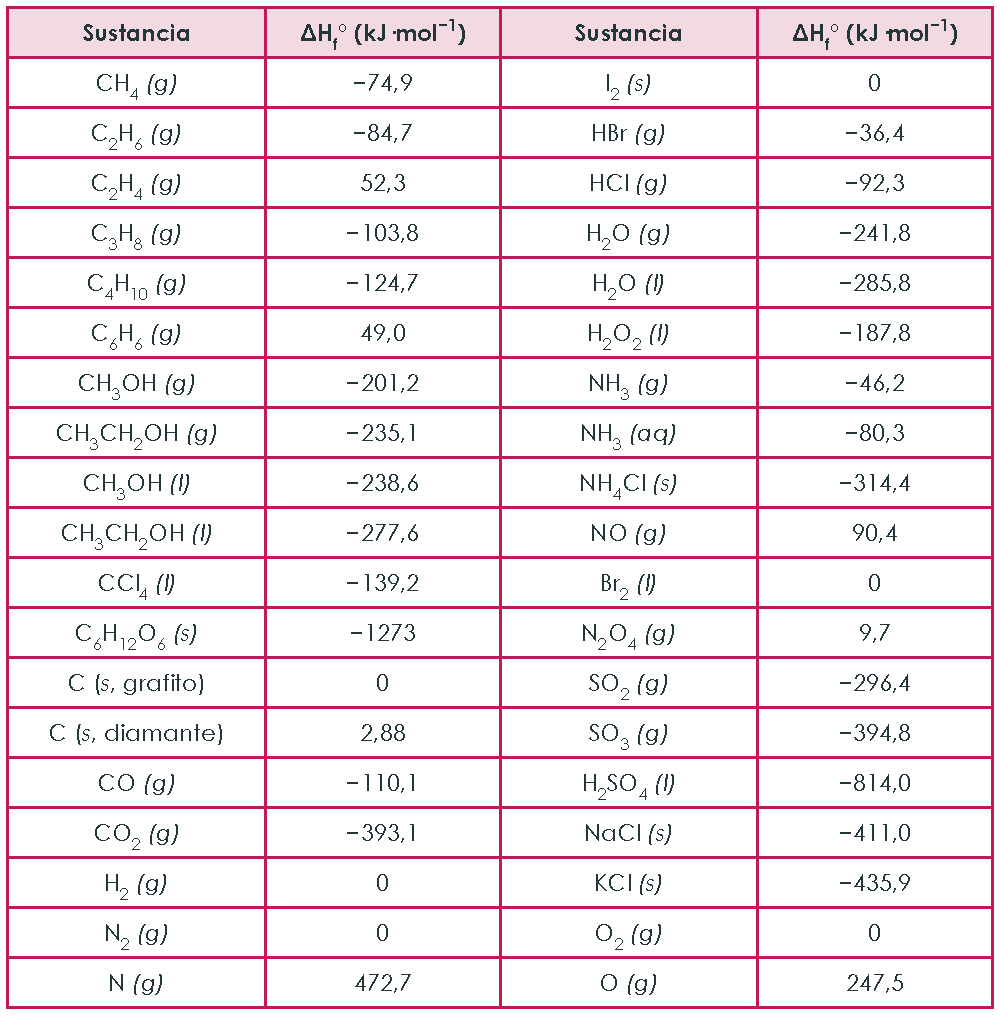
\includegraphics[width=0.8\linewidth]{FigurasSVG/UD4_Termodinamica/pdf/UD4_E04_entalpias_formacion.pdf}
    \caption{Entalpías de formación}
    \label{fig:entalpias_de_formacion}
\end{figure}

\begin{figure}[H]
    \centering
    % [FIGURA ORIGINAL] \includegraphics[scale=.5]{images/imagesUD4Termidonamica/UD4_Problemas/entalpias_de_enlace.png}
    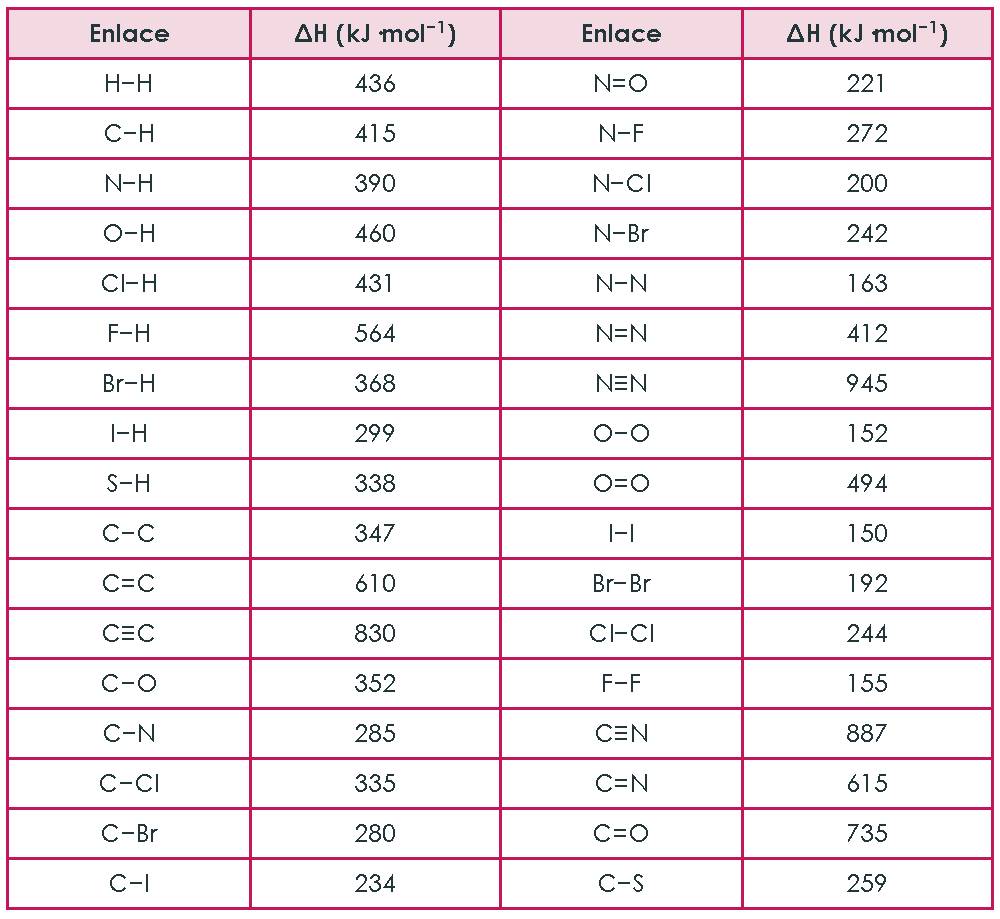
\includegraphics[width=0.75\linewidth]{FigurasSVG/UD4_Termodinamica/pdf/UD4_E05_entalpias_enlace.pdf}
    \caption{Entalpías de enlace}
    \label{fig:entalpias_de_enlace}
\end{figure}



%----------------------------------------------------------------------------------------
%	PART
%----------------------------------------------------------------------------------------


    \part{Cinética Química}

%----------------------------------------------------------------------------------------
%	SECTIONING EXAMPLES CHAPTER
%----------------------------------------------------------------------------------------

    \chapterimage{orange5b.png} % Chapter heading image
    \chapterspaceabove{6.75cm} % Whitespace from the top of the page to the chapter title on chapter pages
    \chapterspacebelow{7.25cm} % Amount of vertical whitespace from the top margin to the start of the text on chapter pages

%------------------------------------------------

    \chapter{Cinética Química}

    \vspace*{18pt}
\section{Cinética química}\label{sec:cinetica-quimica}

\begin{center}
    \begin{definition}[Cinética Química]
        La \rojon{Cinética química} se encarga del estudio de la velocidad de las reacciones químicas y los factores que la afectan.
    \end{definition}
\end{center}

La cinética química relaciona los mecanismos moleculares de ruptura y formación de enlaces tomando en consideración el \negrita{tiempo} a partir de magnitudes macroscópicas y microscópicas.


\section{Velocidad de reacción}\label{sec:velocidad-de-reaccion}

De manera general, podemos decir que la velocidad de reacción nos mide la aparición o desaparición de una sustancia con el tiempo en una reacción química.

\begin{center}
    \begin{definition}[Velocidad Instantánea de Reacción]
        Definimos \rojon{Velocidad instantánea} como la derivada de la concentración de una especie respecto del tiempo y podemos definir la velocidad de desaparición de los reactivos así como la velocidad de aparición de los productos.

        Su unidad, por tanto, será: \unit{\mole\per\litre\per\s} o bien \unit{\m\per\s}
    \end{definition}
\end{center}

Sea una reacción general del tipo:
\begin{centeredequation}
    \ch{a\ A + b\ B -> c\ C + d\ D} \label{eq:general}
\end{centeredequation}

Por tanto, podemos definir tanto las velocidades de desaparición como las velocidades de aparición de la siguiente manera:
\begin{enumerate}[label=\numberballmDarkTeal]
        \item \negsubro{Velocidades de desaparición}: tenemos que poner signo negativo para que la velocidad obtenga un signo positivo debido a que las concentraciones de los reactivos disminuyen con el tiempo.
        \begin{paracol}{2}
            \begin{equation}
                v_A = -\ \dfrac{1}{a}\ \dfrac{d[A]}{dt}\label{eq:velocidad-a}
            \end{equation}
            \switchcolumn
            \begin{equation}
                v_B = -\ \dfrac{1}{b}\ \dfrac{d[B]}{dt}\label{eq:velocidadb}
            \end{equation}
        \end{paracol}
        También lo podemos escribir como:
        \begin{paracol}{2}
            \begin{equation}
                v_A = -\ \dfrac{1}{a}\ \dfrac{\Delta[A]}{\Delta t}\label{eq:velocidad-a-incremento}
            \end{equation}
            \switchcolumn
            \begin{equation}
                v_B = -\ \dfrac{1}{b}\ \dfrac{\Delta[B]}{\Delta t}\label{eq:velicudad-b-incremento}
            \end{equation}
        \end{paracol}
        \item \negsubro{Velocidad de aparición}: se hace tomando como referencia los productos quedando por tanto sus velocidades como:
        \begin{paracol}{2}
            \begin{equation}
                v_C = +\ \dfrac{1}{c}\ \dfrac{d[C]}{dt}\label{eq:velocidad-c}
            \end{equation}
            \switchcolumn
            \begin{equation}
                v_D= +\ \dfrac{1}{d}\ \dfrac{d[D]}{dt}\label{eq:velocidadd-d}
            \end{equation}
        \end{paracol}
        o bien,
        \begin{paracol}{2}
            \begin{equation}
                v_C = +\ \dfrac{1}{c}\ \dfrac{\Delta[C]}{\Delta t}\label{eq:velocidad-c-incremento}
            \end{equation}
            \switchcolumn
            \begin{equation}
                v_D= +\ \dfrac{1}{d}\ \dfrac{\Delta [D]}{\Delta t}\label{eq:velocidad-d-incremento}
            \end{equation}
        \end{paracol}
        Las concentraciones de los productos a diferencia de los reactivos aumentan con el tiempo.
\end{enumerate}
A continuación, tenemos la representación de como varía la concentración de las especies con el tiempo de la reacción:
\begin{centeredequation}
    \ch{H2 + I2 -> 2 HI}
\end{centeredequation}

\begin{figure}[h]
    \centering
    % [FIGURA ORIGINAL] \includegraphics[scale=.5]{images/imagesUD5CineticaQuimica/UD5_Teoria/velocidadreaccion}
    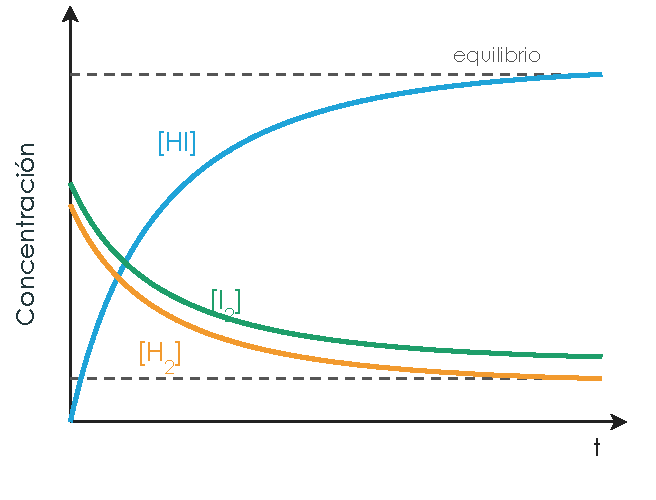
\includegraphics[width=0.55\linewidth]{FigurasSVG/UD5_Cinetica_Quimica/pdf/UD5_01_velocidad_reaccion_HI.pdf}
    \caption{Variación de las concentraciones de reactivos y productos con relación al tiempo en la reacción de hidrógeno molecular con yodo molecular}
    \label{fig:velocidadreaccion}
\end{figure}

Al introducir estos coeficientes estequiométricos en la velocidad conseguimos que \ul{la velocidad calculada respecto a cualquier reactivo o producto sea la misma}, es decir:
\begin{equation}
    v = -\ \dfrac{1}{a}\ \dfrac{d[A]}{dt} =  -\ \dfrac{1}{b}\ \dfrac{d[B]}{dt} =  \dfrac{1}{c}\ \dfrac{d[C]}{dt} =   \dfrac{1}{d}\ \dfrac{d[D]}{dt}\label{eq:velocidad-todas}
\end{equation}

Con esto en lugar de velocidades de reacción referidas a un reactivo o un producto podemos hablar de una única velocidad de reacción.

Por ejemplo, veamos la obtención de metanal a partir de metanol según la ecuación:
\begin{center}
    \ch{2 CH3OH\ (g) + O2\ (g) -> 2 HCOH\ (g) + 2 H2O\ (g) }
\end{center}
La velocidad calculada a partir de cualquier reactivo sería:
\begin{centeredequation}
    v = -\ \dfrac{1}{2}\ \dfrac{d[\ch{CH3OH}]}{dt} =  -\  \dfrac{d[\ch{O2}]}{dt} =  \dfrac{1}{2}\ \dfrac{d[\ch{HCHO}]}{dt} =   \dfrac{1}{2}\ \dfrac{d[\ch{H2O}]}{dt}\label{eq:velocidad-todas-ejemplo}
\end{centeredequation}

\negsubro{IMPORTANTE:} la velocidad al ser una magnitud tendrá, por tanto, su unidad.
La concentración se suele representar en \si{\mole\per\litre}.
Si el tiempo lo tenemos en segundos, tendremos, en consecuencia, que la unidad de la velocidad será: \si{\mole\per\litre\per\s}  o lo que es lo mismo \si{\mole\litre^{-1}\s^{-1}}


\section{Ecuación de velocidad}\label{sec:ecuacion-de-velocidad}

Las velocidades vistas anteriormente las podemos expresar mediante una ecuación a la que denominaremos \azuln{ecuación de velocidad} que expresa la velocidad de una reacción en un determinado instante en función de las concentraciones de las sustancias presentes en ese momento.
Si consideramos la reacción general de la expresión \eqref{eq:general} tendríamos:
\begin{centeredequation}
    v = K\ [A]^\alpha\ [B]^\beta\label{eq:ecuacion-velocidad-general}
\end{centeredequation}

\vspace*{-6pt}
siendo:
\begin{itemize}
    \item La constante $\bm{k}$ se llama \azuln{constante de velocidad}.
    Esta constante tendrá unidades y sus unidades dependerán del orden total o global de la reacción (ver más adelante)
    \item Los exponentes $\bm{\alpha}$ y $\bm{\beta}$ a los que están elevadas las concentraciones de los reactivos se llama \azuln{órdenes parciales de reacción}.
    \item A la suma de $\bm{\alpha}$ y $\bm{\beta}$ se le conoce como \azuln{orden total} o \azuln{orden global}  de la reacción.
    \item Las unidades de la constante de velocidad $\bm{k}$ dependerán, por tanto, del orden global de la reacción.
    \item Conociendo las unidades de la constante de velocidad \( \bm{k} \) podemos obtener fácilmente el orden global de la reacción.
    \item A un mayor valor de $\bm{k}$ la velocidad de reacción será mayor.
\end{itemize}

\negsubro{IMPORTANTE}: los órdenes parciales de reacción no deben confundirse con los coeficientes estequiométricos ($a\ , b\ , c\ , d\ $) y se deben calcular de manera independiente.
Es cierto que cuando una reacción es \azuln{elemental} (más adelante se verá lo que es una reacción elemental) los órdenes parciales y los coeficientes estequiométricos coinciden.

Como podemos ver en la ecuación \eqref{eq:ecuacion-velocidad-general}, solo aparecen los reactivos mientras que los productos han desaparecido.
En la ecuación de velocidad solo tendremos en cuenta la concentración de los reactivos.

\subsection{Ecuación de velocidad de los casos más significativos}\label{sec:casos_significativos}

Consideremos un caso muy simple en el que tenemos una reacción del tipo:
\begin{centeredequation}
    \ch{A -> Productos}
\end{centeredequation}

y además, consideraremos que la reacción que se produce es elemental de modo que podemos escribir que  $v = k\ [A]^\alpha $ o bien $v = - \dfrac{d[A]}{dt}$.
Si igualamos ambas expresiones tendremos que:
\begin{centeredequation}
    k\ [A]^\alpha = - \dfrac{d[A]}{dt}
\end{centeredequation}
reorganizando términos tendremos que:
\begin{centeredequation}
    \dfrac{d[A]}{[A]^\alpha} = -k\  dt
\end{centeredequation}

Si integramos entre el instante $t=0$ donde tendremos una concentración de $A$ de $[A]_0$ y entre el instante $t$ donde la concentración de $A$ es de $[A]_t$ tendremos que:
\begin{centeredequation}
    \int_{[A]_0}^{[A]_t} \dfrac{d[A]}{[A]^\alpha}= -k\int_{t_0}^{t} dt
\end{centeredequation}

\begin{enumerate}[label=\numberballmDarkTeal]
        \item \negsubro{Orden cero}. $\alpha = 0$.
        Tendremos que:
        \begin{equation}
            [A]
            _t = [A]_0 -K\ t\label{eq:cinetica-orden-cero}
        \end{equation}
        Si representamos $[A]$ frente el tiempo tendremos una gráfica lineal del tipo:
        \begin{figure}[H]
            \centering
            % [FIGURA ORIGINAL] \includegraphics[scale=.5]{images/imagesUD5CineticaQuimica/UD5_Teoria/ordencero}
            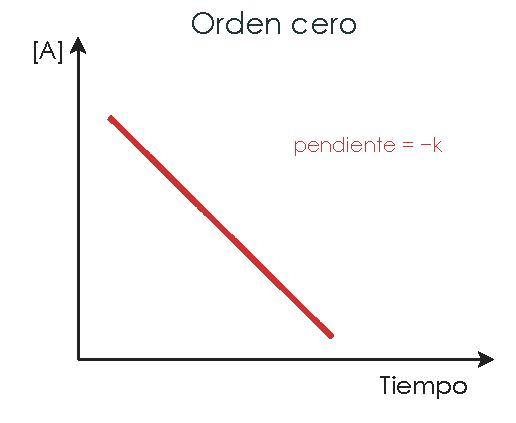
\includegraphics[width=0.45\linewidth]{FigurasSVG/UD5_Cinetica_Quimica/pdf/UD5_02_orden_cero.pdf}
            \caption{Cinética de orden cero}
            \label{fig:ordencero}
        \end{figure}
        \item \negsubro{Orden uno}. $\alpha = 1$.
        Tendremos que:
        \begin{equation}
            [A]
            _t = [A]_0\ e^{-K\ t}\label{eq:cinetica-orden-uno}
        \end{equation}
        esta ecuación la podríamos escribir como:
        \begin{equation*}
            [A]
            _t = [A]_0\ \exp\left(-K\ t\right)\label{eq:cinetica-orden-uno-integrada}
        \end{equation*}
        Si tomamos logaritmos neperianos
        \begin{equation}
            \ln [A]_t = \ln [A]_0 - K\ t\label{eq:cinetica-orden-uno-ln}
        \end{equation}
        Si representamos $\ln [A]$ frente el tiempo tendremos una gráfica lineal del tipo:
        \begin{figure}[H]
            \centering
            % [FIGURA ORIGINAL] \includegraphics[scale=.5]{images/imagesUD5CineticaQuimica/UD5_Teoria/ordenuno}
            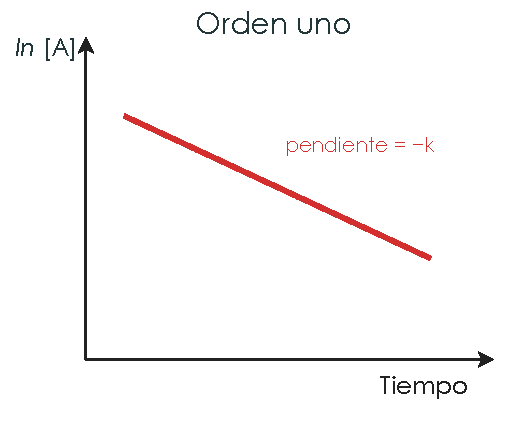
\includegraphics[width=0.45\linewidth]{FigurasSVG/UD5_Cinetica_Quimica/pdf/UD5_03_orden_uno.pdf}
            \caption{Cinética de orden uno}
            \label{fig:ordenuno}
        \end{figure}
        \item \negsubro{Orden dos}. $\alpha = 2$.
        Tendremos que:
        \begin{equation}
            \dfrac{1}{[A]_t} - \dfrac{1}{[A]_0} = k\ t\label{eq:cinetica-orden-dos}
        \end{equation}
        Reagrupando la ecuación la podemos escribir como:
        \begin{equation}
            \dfrac{1}{[A]_t}  =  \dfrac{1}{[A]_0} + k\ t  \label{eq:cinetica-orden-dos-ordenada}
        \end{equation}
%          \begin{equation}
%              [A]_t = \dfrac{[A]_0}{1 + [A]_0\ k\ t}\label{eq:cinetica-orden-dos-integrada}
%          \end{equation}
        Si representamos $\frac{1}{[A]}$ frente el tiempo tendremos una gráfica lineal del tipo:
        \begin{figure}[H]
            \centering
            % [FIGURA ORIGINAL] \includegraphics[scale=.5]{images/imagesUD5CineticaQuimica/UD5_Teoria/ordendos}
            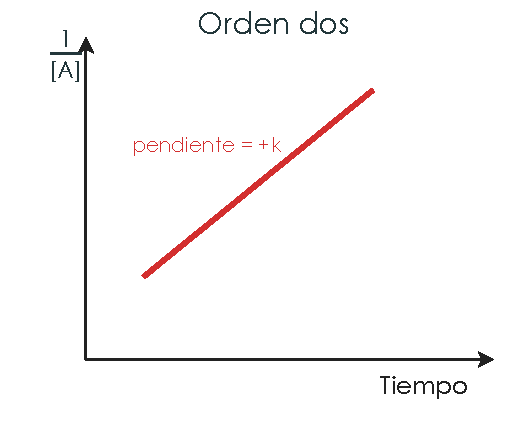
\includegraphics[width=0.45\linewidth]{FigurasSVG/UD5_Cinetica_Quimica/pdf/UD5_04_orden_dos.pdf}
            \caption{Cinética de orden dos}
            \label{fig:ordendos}
        \end{figure}
\end{enumerate}


\begin{enumerate}
    \item Todas las gráficas mostradas consiste en una línea recta, eso es así para obtener con facilidad los parámetros que necesitamos.
    \item Debemos fijarnos en lo que se representa en el eje \( y \) ya que en el eje \( x \) siempre tendremos el tiempo.
\end{enumerate}

\subsection{Cálculo de las órdenes parciales y orden global de la reacción}\label{subsec:calculo-de-las-ordenes-parciales-y-orden-global-de-la-reaccion}

\subsubsection{Método de las velocidades iniciales}

Es el método más utilizado y muy útil, ya que nos permite obtener los órdenes parciales y el orden global de la reacción, así como la constante de velocidad.
Para su explicación veamos el siguiente ejemplo:

Sea la reacción:
\begin{centeredequation}
    \ch{CO\ (g) + NO2\ (g) -> CO2\ (g) + NO\ (g) }
\end{centeredequation}

De esta reacción nos dan los siguientes datos experimentales:
%\begin{table}[H]
%    \centering
%    \begin{tblr}{|c|c|c|c|}
%        \hline
%        \negrita{Experiencia} & $[\ch{CO}]_0$ (\si{\mole\per\litre}) & $[\ch{NO2}]_0$ (\si{\mole\per\litre}) & $v_0$ (\si{\mole\per\litre\per\s}) \\
%        \hline
%        1                     & \num{2e-4}                           & \num{0.5e-4}                          & \num{1.9e-8}                       \\
%        \hline
%        2                     & \num{2e-4}                           & \num{1.0e-4}                          & \num{3.8e-8}                       \\
%        \hline
%        3                     & \num{4e-4}                           & \num{0.5e-4}                          & \num{3.8e-8}                       \\
%        \hline
%    \end{tblr}\label{tab:table-ejemplo-orden-de-reaccion}
%\end{table}
\begin{table}[H]
    \centering
    \caption{Tabla con velocidades iniciales de reacción y concentraciones}
    \vspace{-5pt}
    \begin{tabular}{@{}lccc@{}}
        \toprule
        \textbf{Exp.} & \textbf{$[\ch{CO}]_0$ (\si{\mole\per\litre})} & \textbf{$[\ch{NO2}]_0$ (\si{\mole\per\litre})}         & \textbf{$v_0$ (\si{\mole\per\litre\per\s})}               \\
        \midrule
        1             & \num{2e-4}                                    & \num{0.5e-4}                                   & \num{1.9e-8}  \\[3pt]
        2             & \num{2e-4}                                    & \num{1.0e-4}                                   & \num{3.8e-8} \\[3pt]
        3             & \num{4e-4}                                    & \num{0.5e-4}                                   & \num{3.8e-8}                                \\
        \bottomrule
    \end{tabular}
    \label{tab:}
\end{table}
Primero lo que debemos hacer es poner la ecuación de la velocidad que en este caso sería:
\begin{centeredequation}
    v = k\ [\ch{CO}]^\alpha \ [\ch{NO2}]^\beta
\end{centeredequation}

Como podemos ver, para escribir la ecuación de velocidad, debemos poner \(v\), igualarla a la correspondiente constante de velocidad \(k\) y multiplicarla por la concentración de los REACTIVOS elevada a sus correspondientes órdenes de reacción (en este caso parciales).

Como lo que nos dan son velocidades iniciales, podemos escribir la expresión anterior de la siguiente manera:
\begin{centeredequation}
    v_0 = k\ [\ch{CO}]_0^\alpha \ [\ch{NO2}]_0^\beta
\end{centeredequation}

Como tenemos tres experimentos, podemos plantear entonces que:


    \begin{gather*}
        v_{01} = k\ [\ch{CO}]_{01}^\alpha \ [\ch{NO2}]_{01}^\beta \separ
        v_{02} = k\ [\ch{CO}]_{02}^\alpha \ [\ch{NO2}]_{02}^\beta \separ
        v_{03} = k\ [\ch{CO}]_{03}^\alpha \ [\ch{NO2}]_{03}^\beta \separ
    \end{gather*}
Si dividimos las velocidades $v_{01}$ y $v_{02}$ podemos ver como la concentración del monóxido de carbono desaparece quedando tan solo la del dióxido de nitrógeno, permitiendo así obtener $\beta$.
\begin{gather*}
    \dfrac{v_{01}}{v_{02}} = \dfrac{k\ [\ch{CO}]_{01}^\alpha \ [\ch{NO2}]_{01}^\beta}{k\ [\ch{CO}]_{02}^\alpha \ [\ch{NO2}]_{02}^\beta}\separ
    \dfrac{v_{01}}{v_{02}} = \dfrac{k\ [(\num{2e-4})^\alpha \ [(\num{0.5e-4})^\beta}{k\ [(\num{2e-4})^\alpha \ [(\num{1.0e-4})^\beta}
\end{gather*}
Si operamos tendremos que:
\begin{gather*}
    \dfrac{\num{1.9e-8}}{\num{3.8e-8}} = \dfrac{k\ [\ch{CO}]_{01}^\alpha \ [\ch{NO2}]_{01}^\beta}{k\ [\ch{CO}]_{02}^\alpha \ [\ch{NO2}]_{02}^\beta}\separ
    \dfrac{\num{1.9e-8}}{\num{3.8e-8}} = \dfrac{\cancelred{k}\ \cancelred{[(\num{2e-4})^\alpha} \ [(\num{0.5e-4})^\beta}{\cancelred{k}\ \cancelred{[(\num{2e-4})^\alpha} \ [(\num{1.0e-4})^\beta}\separ
    \dfrac{1}{2} = \left( \dfrac{1}{2} \right)^\beta\separ
    0.5 = 0.5^\beta \separ
    \beta = \log_{0.5}(0.5)\separ
    \tcboxmath[opteqA]{\beta = 1}
\end{gather*}
Si en vuestra calculadora no podéis poner los logaritmos con la base que salga, podéis hacer un cambio de base según (siendo $c$ la nueva base):
\begin{equation*}
    log_{b}(x) = \dfrac{log_{c}(x)}{log_{c}(b)}
\end{equation*}
Si ahora hacemos un tratamiento similar, pero dividiendo $v_{01}$ y $v_{03}$ obtendríamos el valor de $\alpha = 1$.
Para obtener el valor del orden total de la reacción tendremos que sumar $\alpha$ y $\beta$ siendo en este caso $2$.

Para obtener el valor de la constante de velocidad, solo tenemos que irnos a cualquier expresión de la velocidad y sustituir los valores de las órdenes parciales de reacción por su valor, obteniendo finalmente que $k = 1.9\ \si{\mole^{-1}\litre\s^{-1}}$ es decir $k = \SI{1.9}{\litre\per\mole\per\s}$

\subsubsection{Método gráfico}
Consiste en realizar representaciones gráficas según las ecuaciones vistas en el apartado \ref{sec:casos_significativos} y ver qué gráficas encajan mejor según el orden de reacción.


\section{Reacciones directas e inversas}

Hasta ahora hemos visto siempre la reacción directa, es decir el paso en el que los reactivos $A$ y $B$ pasan a los productos $C$ y $D$.
Sin embargo, en ocasiones esos productos cuando se van formando, vuelven a reaccionar entre sí para dar de nuevo los reactivos de partida.
A esta reacción entre los productos para dar de nuevo los reactivos se denomina \azuln{reacción inversa}.
Cuando tenemos un caso así, se suele representar con una doble flecha de la siguiente manera:
\begin{centeredequation}
    \ch{a\ A + b\ B <=> [reacción\ directa\ (d)][reacción\ inversa\ (i)] c\ C + d\ D} \label{eq:general_equilibrio}
\end{centeredequation}

Ambas velocidades quedarían, por tanto:
\begin{paracol}{2}
    \begin{equation*}
        v_d = k_d\ [A]^a\ [B]^b
    \end{equation*}
    \switchcolumn
    \begin{equation*}
        v_i = k_i\ [C]^c\ [D]^d
    \end{equation*}
\end{paracol}
En este caso, podemos poner los coeficientes estequiométricos como órdenes parciales de reacción porque nos encontramos en una reacción elemental en cada sentido.

Cuando las velocidades de la reacción directa se igualan con las velocidades de la reacción inversa se dice que se alcanza el \rojon{equilibrio químico} y al cociente entre ambas constantes de velocidad se le denomina \rojon{constante de equilibrio químico}
\begin{gather*}
    v_d = v_i\separ
    k_d\ [A]^a\ [B]^b = k_i\ [C]^c\ [D]^d
\end{gather*}
Podemos deducir que:
\begin{centeredequation}
    \dfrac{k_d}{k_i} = \dfrac{[C]^c\ [D]^d}{[A]^a\ [B]^b}
\end{centeredequation}
Por lo tanto
\begin{centeredequation}
    k_{\text{equilibrio}} = \dfrac{k_d}{k_i}
\end{centeredequation}

Y también podemos decir que:
\begin{centeredequation}
    k_{\text{equilibrio}} = \dfrac{[C]^c\ [D]^d}{[A]^a\ [B]^b}
\end{centeredequation}

\begin{figure}[H]
    \centering
    % [FIGURA ORIGINAL] \includegraphics[scale=.5]{images/imagesUD5CineticaQuimica/UD5_Teoria/equilibrio_cinetica}
    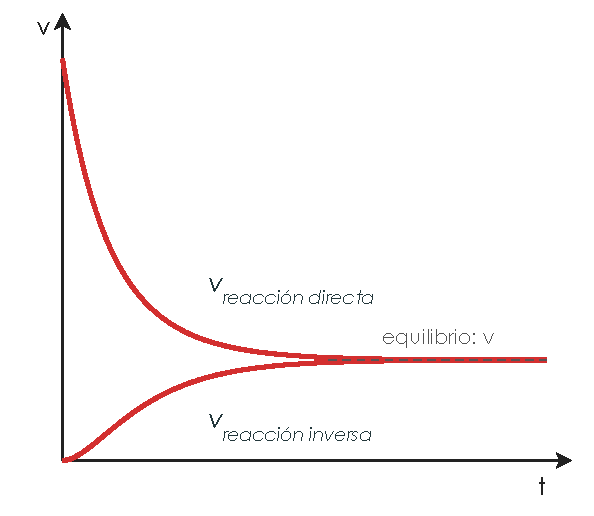
\includegraphics[width=0.5\linewidth]{FigurasSVG/UD5_Cinetica_Quimica/pdf/UD5_05_equilibrio_velocidades.pdf}
    \caption{Equilibrio químico}
    \label{fig:equilibrio_cinetica.png}
\end{figure}


\section{Teorías sobre las reacciones químicas}\label{sec:teorias-sobre-las-reacciones-quimicas}

\subsection{Teoría de colisiones}\label{subsec:teoria-de-colisiones}
Esta teoría fue enunciada por Lewis en 1918 y dice:
\begin{ley}[Teoría de colisiones]
    La \rojon{teoría de colisiones} de Lewis propone que las reacciones químicas se producen por choques entre las moléculas
\end{ley}

La velocidad de reacción según esta teoría dependerá, por tanto, de los siguientes factores:
\begin{enumerate}[label=\numberballmDarkTeal]
        \item \azuln{Frecuencia de choque por unidad de volumen}.
        A mayor número de choques, la velocidad de reacción será mayor.
        \item \azuln{Eficacia del choque}.
        Además de tener una alta frecuencia, los choques deben ser lo suficientemente efectivos para que se lleve a cabo la reacción y para ello se necesitará:
        \begin{enumerate}
            \item Los choques deben tener una energía cinética que sea suficiente para romper los enlaces necesarios.
            A esta energía suficiente se le denomina \azuln{energía de activación, $E_a$}.
            \item La fracción de moléculas que tiene esa energía o una energía superior fue calculada por Ludwig Boltzmann y es:
            \begin{centeredequation}
                e^{-\frac{E_a}{R\ T}}
            \end{centeredequation}
            A partir de este momento, esta expresión la escribiremos como:
            \begin{centeredequation}
                \exp\biggl(-\dfrac{E_a}{RT}\biggr)\label{eq:expresion_Boltzman}
            \end{centeredequation}

            \item Orientación adecuada además de tener la suficiente energía.
        \end{enumerate}
\end{enumerate}

Teniendo en cuenta todas estas consideraciones, la \azuln{ecuación de Arrhenius} permite calcular el valor de la constante de velocidad según la expresión:
\begin{centeredequation}
    k = A\ e^{-\frac{E_a}{R T}}\label{eq:Arrhenius}
\end{centeredequation}

La ecuación \eqref{eq:Arrhenius} a partir de ahora la escribiremos de la siguiente forma:
\begin{centeredequation}
    k = A\exp\biggl(-\dfrac{E_a}{RT}\biggr)\label{eq:Arrhenius_b}
\end{centeredequation}

\begin{itemize}
    \item $A$: factor de frecuencia.
    \item $R$: constante de los gases ideales en julios.
    \item $T$: temperatura absoluta, es decir en kelvin.
    \item $E_a$: energía de activación.
\end{itemize}

\subsection{Teoría del estado de transición o complejo activado}\label{subsec:teoria-del-estado-de-transicion-o-complejo-activado}

\negrita{H. Eyring} propuso que cuando las moléculas de los reactivos chocan, se forma una especie intermedia denominada \azuln{complejo activado} o \azuln{complejo de transición}.

\begin{figure}[H]
    \centering
    \subfloat[Exotérmica]{
        % [FIGURA ORIGINAL] \includegraphics[scale=.45]{images/imagesUD5CineticaQuimica/UD5_Teoria/exotermica}
        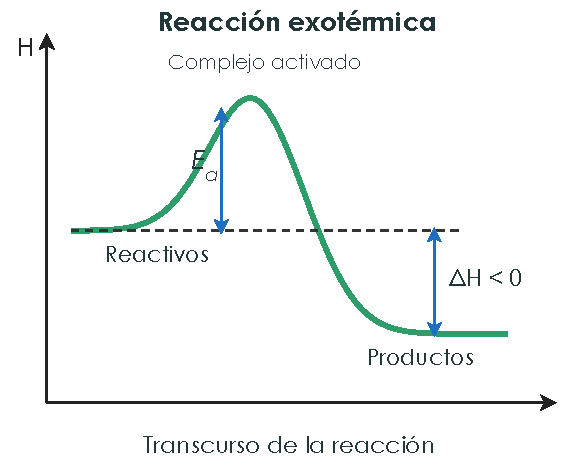
\includegraphics[width=0.31\linewidth]{FigurasSVG/UD5_Cinetica_Quimica/pdf/UD5_06_perfil_exotermica.pdf}
        \label{fig:exotermica}
    }
    \subfloat[Endotérmica]{
        % [FIGURA ORIGINAL] \includegraphics[scale=.45]{images/imagesUD5CineticaQuimica/UD5_Teoria/endotermica}
        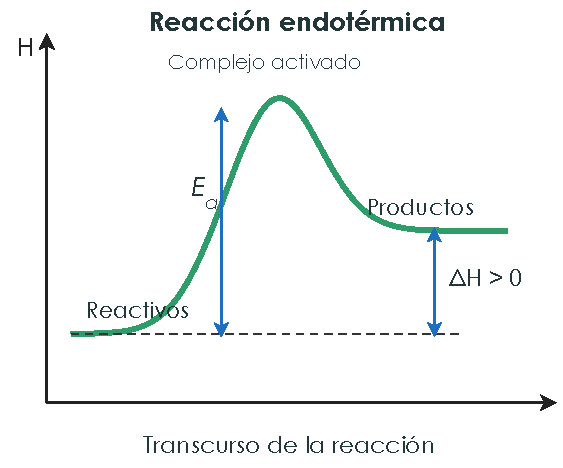
\includegraphics[width=0.31\linewidth]{FigurasSVG/UD5_Cinetica_Quimica/pdf/UD5_07_perfil_endotermica.pdf}
        \label{fig:endotermica}
    }
    \subfloat[Complejo Activado]{
        \vspace*{6pt}
        % [FIGURA ORIGINAL] \includegraphics[scale=.35]{images/imagesUD5CineticaQuimica/UD5_Teoria/complejo_activado}
        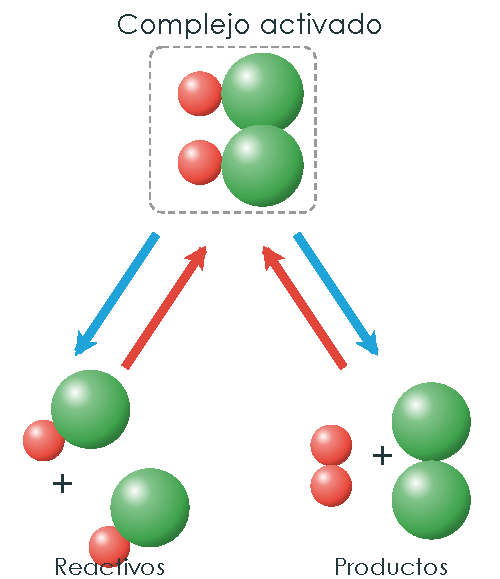
\includegraphics[width=0.25\linewidth]{FigurasSVG/UD5_Cinetica_Quimica/pdf/UD5_08_complejo_activado.pdf}
        \label{fig:complejo_activado}
    }
    \caption{}
\end{figure}


En la imagen, podemos ver como en este caso la energía de activación ($E_a$) es la energía que debemos suministrar para formar dicho complejo activado, así cuanto menor sea la energía más fácil será que las moléculas del reactivo se dispongan para formar dicho complejo y más rápida, por tanto, será la reacción.

Ese complejo activado es una especie de muy alta energía y de una corta duración.


\section{Mecanismo de reacción}\label{sec:mecanismo-de-reaccion}

Existen reacciones que se producen en una sola etapa como:
\begin{center}
    \formula{Cl2 \gas{} + H2 \gas{} -> 2 HCl \gas{}}\\
    \formula{CH3Br \aq{} + OH- \aq{} -> CH3OH \aq{} + Br- \aq{}}
\end{center}

A las reacciones que se producen en una sola etapa se les denomina \rojon{reacciones elementales}.

Sin embargo, muchas reacciones químicas se llevan a cabo en varias etapas.
Cada etapa será una \negrita{reacción elemental}.

\subsection{Velocidad de las etapas elementales y la reacción global}\label{subsec:velocidad-de-las-etapas-elementales-y-la-reaccion-global}
Cuando una reacción se realiza en varias etapas, su velocidad global dependerá de la velocidad de cada etapa o reacción elemental siendo, por tanto, su velocidad la combinación lineal de todas ellas.

Si se diera el caso de que una de esas etapas fuera mucho más lenta que las demás, las velocidades de las otras reacciones se pueden despreciar.
A esta etapa o reacción que determina la velocidad de la reacción global se le denomina \negrita{etapa limitante} o \negrita{etapa controlante de la velocidad}.

Sea por ejemplo la reacción:
\begin{center}
    \formula{NO2 \gas{} + CO \gas{} -> NO \gas{} + CO2 \gas{}}
\end{center}
Esta reacción tiene como ecuación de velocidad $v = k\ [\formula{NO2}]^2$.
A partir de su ecuación de velocidad podemos ver que no se trata de una reacción elemental puesto que no aparece \conc{CO}.
Las etapas propuestas para su mecanismo sería:
\begin{gather*}
    \formula{NO2 \gas{} + NO2 \gas{} -> NO3 \gas{} + NO \gas{}};\quad v_1 = k_1\ \conc{NO2}^2\separ
    \formula{NO3 \gas{} + CO \gas{} -> NO2 \gas{} + CO2 \gas{}};\quad v_2 = k_2\ \conc{NO3}\ \conc{CO}
\end{gather*}
La primera etapa es mucho más lenta que la segunda y, por tanto, actúa como etapa limitante pudiéndose descartar la segunda reacción.
Como vemos también el mecanismo de reacción, en la reacción global no aparece el \conc{NO3}, esto es debido a que es un \negrita{intermedio de reacción}, es decir es una especie que no está presente ni en los reactivos ni en los productos, pero que se forma y desaparece durante el proceso.

\subsection{Molecularidad}\label{subsec:molecularidad}

Llamamos \negrita{molecularidad} al número de moléculas de reactivos que colisionan simultáneamente para formar el complejo activado de una reacción elemental.
Generalmente, coinciden con el orden de reacción aunque no siempre.

Por norma general las reacciones suelen ser \negrita{unimoleculares} (una especie) o \negrita{bimuleculares} (dos especies)

\begin{itemize}
    \item \negsubro{Reacción elemental unimolecular}
    \begin{equation*}
        \formula{A -> Productos};\quad v= k\ \conc{A}
    \end{equation*}
    \item \negsubro{Reacción elemental bimolecular}
    \begin{equation*}
        \formula{A + B -> Productos};\quad v= k\ \conc{A}\ \conc{B}
    \end{equation*}
\end{itemize}


\section{Factores que influyen en la velocidad de reacción}\label{sec:factores-que-influyen-en-la-velocidad-de-reaccion}

La velocidad de una reacción química depende de múltiples factores y que de alguna manera pueden aparecer en la ecuación de velocidad.
Estos factores son:

\begin{enumerate}[label=\numberballmDarkTeal]
        \item \negsubro{Concentración de los reactivos}.
        Como ya hemos visto en la ecuación de la velocidad, la concentración de los reactivos es directamente proporcional a la velocidad, por lo que podemos decir que:
        \caja{Un aumento en la concentración de los reactivos conlleva un aumento de la velocidad}
        \item \negsubro{Efecto de la temperatura}.
        Tal y como hemos visto en la expresión de \negrita{Arrhenius} (ecuación \eqref{eq:Arrhenius_b}) si aumentamos la temperatura aumentará la constante de velocidad y al aumentar la constante de velocidad aumentará por tanto la velocidad de reacción.

        Si aumentamos la temperatura, la fracción de moléculas con una energía más elevada aumenta, por lo que será más fácil pasar la barrera de la energía de activación y, por tanto, habrá más moléculas que la superen aumentando así la velocidad de reacción.

        Si tomamos logaritmos neperianos en la expresión de Arrhenius, tendremos que:
        \begin{centeredequation}
            \ln k = \ln A - \dfrac{E_a}{R}\ \dfrac{1}{T} \label{eq:Arrhenius_neperiano}
        \end{centeredequation}

        La ecuación \eqref{eq:Arrhenius_neperiano} corresponde a una ecuación de una línea recta del tipo $y = ax + b$ siendo:
        \begin{gather*}
            a = - \dfrac{E_a}{R}\separ
            b = \ln A
        \end{gather*}
        Si representamos los distintos valores de $\ln k$ frente a $\frac{1}{T}$ podemos calcular gráficamente la energía de activación del proceso.

        De esta ecuación podemos sacar las siguientes conclusiones:
        \begin{itemize}
            \item Las reacciones con $E_a$ pequeñas tienen velocidades que aumentan solo ligeramente con la temperatura.
            \item Las reacciones con $E_a$ elevadas tienen velocidades que dependen fuertemente de la temperatura.
        \end{itemize}
        Si conocemos la constante de velocidad $k$ a una determinada temperatura, $T$, la ecuación de Arrhenius permite conocer la constante de velocidad $k\prima$ a una temperatura distinta $T\prima$ según:
        \begin{gather*}
            \ln k = \ln A - \dfrac{E_a}{R}\ \dfrac{1}{T}\separ
            \ln k\prima = \ln A - \dfrac{E_a}{R}\ \dfrac{1}{T\prima}
        \end{gather*}
        Si restamos ambas ecuaciones y las reordenamos tendremos que:
        \begin{centeredequation}
            \ln\dfrac{k\prima}{k} = \dfrac{E_a}{R}\biggl( \dfrac{1}{T} - \dfrac{1}{T\prima}\biggr)
        \end{centeredequation}

        \item \negsubro{Estado físico de los reactivos}.
        Cuando los reactivos se encuentran en estado gaseoso o en disolución las reacciones son más rápidas que si se encuentran en estado líquido o sólido.
        \item \negsubro{Naturaleza de la reacción}.
        En reacciones covalentes (intervienen sustancias covalentes) la velocidad de reacción suele ser menor, debido a que se necesitan romper y formar nuevos enlaces, que en reacciones de tipo iónico, donde las especies ya se encuentran en disolución estando ya ``rotos'' los enlaces.
        \item \negsubro{Catalizadores}.
        Son sustancias que intervienen en alguna etapa de la reacción, pero no se consumen y, por tanto, no aparecen en la reacción global ajustada.

        Los catalizadores \negrita{modifican} el \negrita{mecanismo} de la reacción y, en consecuencia, modificará la energía de activación modificando así la velocidad de la misma.

        Es importante tener claro que los catalizadores \negrita{no modifican las constantes de los equilibrios}
\end{enumerate}

\begin{example}
    ¿Cuál es el valor de la energía de activación para una reacción si la constante de velocidad se duplica cuando la temperatura aumenta de \temperatura[c]{15} a \temperatura[c]{25}?
\end{example}


% \marcador{Hacer los ejercicios 25, 26, 27, 30 y 31 de la página 191}




    \newpage

    %! Author = Profesor
%! Date = 06/06/2024


\section{Ejercicios}

\subsection{Ejercicios}


\begin{exercise}
    Los siguientes datos de velocidades de reacción se obtuvieron a \temperatura[c]{25} para la siguiente reacción:

    \begin{equation*}
        \ch{2 A + B -> C}
    \end{equation*}

    \begin{table}[H]
        \centering
        % --- tabla antigua ---
        % \begin{tblr}{Q[c,m]|Q[c,m]|Q[c,m]|Q[c,m]}
            % \hline
            % \SetRow{blue!5!white} Exp. & {\(v_{\text{formación}}\) \\ \unit{\Molar\per\minute}} & {\ch{[A]_i} \\ \unit{\Molar}} & {\ch{[B]_i} \\ \unit{\Molar}} \\
            % \hline
            % 1 & \num{4.0e-4} & \num{0.1} & \num{0.1} \\
            % \hline
            % 2 & \num{1.2e-3} & \num{0.3} & \num{0.3} \\
            % \hline
            % 3 & \num{4.0e-4} & \num{0.1} & \num{0.3} \\
            % \hline
            % 4 & \num{8.0e-4} & \num{0.2} & \num{0.4} \\
            % \hline
        % \end{tblr}
        % --- tabla nueva ---
        \begin{tabular}{@{}cccc@{}}
            \toprule
            \textbf{Exp.} & \textbf{\makecell{\(v_{\text{formación}}\) \\ \unit{\Molar\per\minute}}} & \textbf{\makecell{\ch{[A]_i} \\ \unit{\Molar}}} & \textbf{\makecell{\ch{[B]_i} \\ \unit{\Molar}}} \\
            \midrule
            1 & \num{4.0e-4} & \num{0.1} & \num{0.1} \\[3pt]
            2 & \num{1.2e-3} & \num{0.3} & \num{0.3} \\[3pt]
            3 & \num{4.0e-4} & \num{0.1} & \num{0.3} \\[3pt]
            4 & \num{8.0e-4} & \num{0.2} & \num{0.4} \\
            \bottomrule
        \end{tabular}
    \end{table}


% \begin{figure}[H]
%     \centering
%     \includegraphics[scale=.5]{velocidadesinicialesanaya.png}
%     \caption{\negrita{Datos experimentales}}
%     \label{fig:velocidadesinicialesanaya.png}
% \end{figure}

    \begin{enumerate}[label=\letraminuscula]
        \item Determina los órdenes parciales y el orden total de reacción.
        \item Calcula el valor de la constante cinética
    \end{enumerate}

    \begin{solu}

%        \begin{figure}[H]
%            \centering
%            \includegraphics[scale=0.6]{images/imagesUD5CineticaQuimica/UD5_Problemas/ejerciciogeneral01.png}
%        \end{figure}
    \end{solu}

\end{exercise}

\begin{exercise}
    Escribe la ecuación de velocidad de una reacción: \ch{3 A + 2 B + C -> Productos}, para la cual

    \begin{table}[H]
        \centering
        % --- tabla antigua ---
        % \begin{tblr}{Q[c,m]|Q[c,m]|Q[c,m]|Q[c,m]}
            % \hline
            % \SetRow{blue!5!white} [A] & [B]              & [C]              & Velocidad inicial \\
            % \hline
            % \SI{0.4}{\Molar}          & \SI{0.1}{\Molar} & \SI{0.2}{\Molar} & \(v\)             \\
            % \hline
            % \SI{0.4}{\Molar}          & \SI{0.2}{\Molar} & \SI{0.4}{\Molar} & \(8\ v\)          \\
            % \hline
            % \SI{0.2}{\Molar}          & \SI{0.2}{\Molar} & \SI{0.2}{\Molar} & \(v\)             \\
            % \hline
            % \SI{0.4}{\Molar}          & \SI{0.1}{\Molar} & \SI{0.4}{\Molar} & \(4\ v\)          \\
            % \hline
        % \end{tblr}
        % --- tabla nueva ---
        \begin{tabular}{@{}cccc@{}}
            \toprule
            \textbf{[A]} & \textbf{[B]} & \textbf{[C]} & \textbf{Velocidad inicial} \\
            \midrule
            \SI{0.4}{\Molar} & \SI{0.1}{\Molar} & \SI{0.2}{\Molar} & \(v\) \\[3pt]
            \SI{0.4}{\Molar} & \SI{0.2}{\Molar} & \SI{0.4}{\Molar} & \(8\ v\) \\[3pt]
            \SI{0.2}{\Molar} & \SI{0.2}{\Molar} & \SI{0.2}{\Molar} & \(v\) \\[3pt]
            \SI{0.4}{\Molar} & \SI{0.1}{\Molar} & \SI{0.4}{\Molar} & \(4\ v\) \\
            \bottomrule
        \end{tabular}
    \end{table}

    \begin{solu}
%        \begin{figure}[H]
%            \centering
%            \includegraphics[scale=0.6]{images/imagesUD5CineticaQuimica/UD5_Problemas/ejerciciogeneral02.png}
%        \end{figure}
    \end{solu}
\end{exercise}

\begin{exercise}
    Una reacción de un reactivo A con un reactivo B muestra los siguientes datos de velocidad cuando se estudia a diferentes concentraciones de A y de B:
    \begin{table}[H]
        \centering
        % --- tabla antigua ---
        % \begin{tblr}{Q[c,m]|Q[c,m]|Q[c,m]}
            % \hline
            % \SetRow{blue!5!white} [A] & [B]              & Velocidad inicial                  \\
            % \hline
            % \SI{0.1}{\Molar}          & \SI{0.1}{\Molar} & \SI{4e-4}{\mole\per\litre\per\s}   \\
            % \hline
            % \SI{0.2}{\Molar}          & \SI{0.1}{\Molar} & \SI{1.6e-3}{\mole\per\litre\per\s} \\
            % \hline
            % \SI{0.5}{\Molar}          & \SI{0.1}{\Molar} & \SI{1e-2}{\mole\per\litre\per\s}   \\
            % \hline
            % \SI{0.5}{\Molar}          & \SI{0.5}{\Molar} & \SI{1e-2}{\mole\per\litre\per\s}   \\
            % \hline
        % \end{tblr}
        % --- tabla nueva ---
        \begin{tabular}{@{}ccc@{}}
            \toprule
            \textbf{[A]} & \textbf{[B]} & \textbf{Velocidad inicial} \\
            \midrule
            \SI{0.1}{\Molar} & \SI{0.1}{\Molar} & \SI{4e-4}{\mole\per\litre\per\s} \\[3pt]
            \SI{0.2}{\Molar} & \SI{0.1}{\Molar} & \SI{1.6e-3}{\mole\per\litre\per\s} \\[3pt]
            \SI{0.5}{\Molar} & \SI{0.1}{\Molar} & \SI{1e-2}{\mole\per\litre\per\s} \\[3pt]
            \SI{0.5}{\Molar} & \SI{0.5}{\Molar} & \SI{1e-2}{\mole\per\litre\per\s} \\
            \bottomrule
        \end{tabular}
    \end{table}

    Halla: a) El orden respecto a A, respecto a B y el orden global de la reacción.
    b) El valor de la constante de velocidad.
    c) Su ecuación de velocidad.
    d) Velocidad cuando [A] y [B] valen \SI{0.3}{\Molar}

    \begin{solu}

%        \begin{figure}[H]
%            \centering
%            \includegraphics[scale=0.6]{images/imagesUD5CineticaQuimica/UD5_Problemas/ejerciciogeneral03}
%        \end{figure}

    \end{solu}
\end{exercise}

\begin{exercise}
    A partir de los datos siguientes, calcula la constante de velocidad y comprueba que la reacción es de primer orden:

    \begin{equation*}
        \ch{2 N2O5 -> 4 NO2 + O2}
    \end{equation*}

    \begin{table}[H]
        \centering
        % --- tabla antigua ---
        % \begin{tblr}{Q[c,m]|Q[c,m]|Q[c,m]|Q[c,m]|Q[c,m]|Q[c,m]}
            % \hline
            % \SetColumn{blue!5!white} t (\unit{\minute}) & \num{0}   & \num{67}  & \num{133} & \num{200} & \num{267}  \\
            % \hline
            % \ch{[N2O5]} \SI{e-3}{\Molar}                & \num{2.6} & \num{1.5} & \num{0.9} & \num{0.5} & \num{0.3} \\
            % \hline
        % \end{tblr}
        % --- tabla nueva ---
        \begin{tabular}{@{}cccccc@{}}
            \toprule
            \SetColumn{blue!5!white} t (\unit{\minute}) & \num{0} & \num{67} & \num{133} & \num{200} & \num{267} \\[3pt]
            \ch{[N2O5]} \SI{e-3}{\Molar} & \num{2.6} & \num{1.5} & \num{0.9} & \num{0.5} & \num{0.3} \\
            \bottomrule
        \end{tabular}
    \end{table}

    \begin{solu}

%        \begin{figure}[H]
%            \centering
%            \includegraphics[scale=0.6]{images/imagesUD5CineticaQuimica/UD5_Problemas/ejerciciogeneral04.png}
%        \end{figure}

    \end{solu}

\end{exercise}

\begin{exercise}
    A partir de los datos siguientes, calcula la constante de velocidad y comprueba que la reacción es de segundo orden:

    \begin{equation*}
        \ch{2 HI -> H2 + I2}
    \end{equation*}

    \begin{table}[H]
        \centering
        % --- tabla antigua ---
        % \begin{tblr}{Q[c,m]|Q[c,m]|Q[c,m]|Q[c,m]|Q[c,m]|Q[c,m]}
            % \hline
            % \SetColumn{blue!5!white} t (\unit{\minute}) & \num{0}   & \num{16.67} & \num{33.3} & \num{50} & \num{66.7}  \\
            % \hline
            % \ch{[HI]} \SI{e-3}{\Molar}                  & \num{200} & \num{120}   & \num{61}   & \num{41} & \num{31}   \\
            % \hline
        % \end{tblr}
        % --- tabla nueva ---
        \begin{tabular}{@{}cccccc@{}}
            \toprule
            \SetColumn{blue!5!white} t (\unit{\minute}) & \num{0} & \num{16.67} & \num{33.3} & \num{50} & \num{66.7} \\[3pt]
            \ch{[HI]} \SI{e-3}{\Molar} & \num{200} & \num{120} & \num{61} & \num{41} & \num{31} \\
            \bottomrule
        \end{tabular}
    \end{table}

    \begin{solu}

%        \begin{figure}[H]
%            \centering
%            \includegraphics[scale=0.6]{images/imagesUD5CineticaQuimica/UD5_Problemas/ejerciciogeneral05.png}
%        \end{figure}

    \end{solu}

\end{exercise}

\begin{exercise}
    Una reacción duplica su constante de velocidad cuando pasa de \temperatura[c]{25} a \temperatura[c]{50}.
    Calcula el valor de su energía de activación.

    \begin{solu}

        Aplicamos la ecuación de Arrhenius en su forma integrada entre dos temperaturas:

        \begin{equation*}
            \ln \left( \dfrac{k_2}{k_1} \right) = \dfrac{E_a}{R} \left( \dfrac{1}{T_1} - \dfrac{1}{T_2} \right)
        \end{equation*}

        Con \(T_1 = \temperatura[k]{298}\), \(T_2 = \temperatura[k]{323}\) y \(k_2 = 2\, k_1\) (la constante se duplica), tenemos:

        \begin{equation*}
            \ln(2) = \dfrac{E_a}{R} \left( \dfrac{1}{298} - \dfrac{1}{323} \right)
        \end{equation*}

        Calculamos el paréntesis:

        \begin{equation*}
            \dfrac{1}{298} - \dfrac{1}{323} = 0,0033557 - 0,0030960 = \SI{2.597e-4}{\per\kelvin}
        \end{equation*}

        Despejando \(E_a\):

        \begin{equation*}
            E_a = \dfrac{R \ln(2)}{2,597 \times 10^{-4}} = \dfrac{8,314 \times 0,6931}{2,597 \times 10^{-4}} = \SI{22185}{\joule\per\mole} \approx \energia[kjmol]{22.2}
        \end{equation*}

    \end{solu}
\end{exercise}

\begin{exercise}
    Una reacción tiene una energía de activación de \energia[j]{9e4} y a 30 °C, su constante de velocidad vale \num{8.9e-3}.
    ¿A qué temperatura será \(k = \SI{1e-2}{\litre\per\mole\per\s}\)?

    \begin{solu}

        Aplicamos la ecuación de Arrhenius entre dos temperaturas:

        \begin{equation*}
            \ln \left( \dfrac{k_2}{k_1} \right) = \dfrac{E_a}{R} \left( \dfrac{1}{T_1} - \dfrac{1}{T_2} \right)
        \end{equation*}

        Con \(T_1 = \temperatura[k]{303}\), \(k_1 = \num{8.9e-3}\), \(k_2 = \num{1e-2}\) y \(E_a = \SI{9e4}{\joule\per\mole}\):

        \begin{equation*}
            \ln \left( \dfrac{0,01}{0,0089} \right) = \ln(1,1236) = 0,1165
        \end{equation*}

        \begin{equation*}
            0,1165 = \dfrac{90\,000}{8,314} \left( \dfrac{1}{303} - \dfrac{1}{T_2} \right) = 10\,825,6 \left( \dfrac{1}{303} - \dfrac{1}{T_2} \right)
        \end{equation*}

        Despejando el paréntesis:

        \begin{equation*}
            \dfrac{1}{303} - \dfrac{1}{T_2} = \dfrac{0,1165}{10\,825,6} = 1,076 \times 10^{-5}
        \end{equation*}

        \begin{equation*}
            \dfrac{1}{T_2} = \dfrac{1}{303} - 1,076 \times 10^{-5} = 0,0033003 - 0,0000108 = 0,0032896
        \end{equation*}

        \begin{equation*}
            T_2 = \dfrac{1}{0,0032896} = \SI{304.0}{\kelvin} \approx \temperatura[c]{31}
        \end{equation*}

        La constante de velocidad alcanzará el valor \(k = \SI{1e-2}{\litre\per\mole\per\s}\) a una temperatura de, aproximadamente, \(\SI{304}{\kelvin}\) (\SI{31}{\celsius}).

    \end{solu}
\end{exercise}

\begin{exercise}
    La constante de velocidad de una reacción se expresa según: \(k = A\ e^{\dfrac{-E_a}{R\ T}}\).
    Indica y razona:
    \begin{enumerate}[label=\letraminuscula]
        \item Unidades y significado de cada término.
        \item ¿Qué término se modifica por un catalizador?
        \item La reacción transcurre mediante etapas elementales cuyas energías de activación son: \(E_{a1} = 93\ ; E_{a2} = 148\ ; E_{a3} = 73\).
        ¿Cuál será la etapa más lenta?
        \item ¿Qué
        influencia ejercerá la temperatura?
    \end{enumerate}

    \begin{solu}

        \textbf{a) Unidades y significado de cada término}

        \begin{itemize}
            \item \(k\): constante de velocidad. Su significado es la constante de proporcionalidad entre la velocidad de reacción y las concentraciones de los reactivos elevadas a sus respectivos órdenes parciales. Sus unidades dependen del orden total de la reacción (por ejemplo, \(\si{\s^{-1}}\) para orden 1, \(\si{\litre\per\mole\per\s}\) para orden 2, etc.).
            \item \(A\): factor de frecuencia o factor preexponencial. Está relacionado con la frecuencia de los choques entre las moléculas de reactivos y con la orientación favorable de dichos choques. Tiene las mismas unidades que \(k\).
            \item \(E_a\): energía de activación. Es la energía mínima que deben poseer las moléculas al chocar para que la colisión sea efectiva y se forme el complejo activado. Se expresa en unidades de energía por mol, \(\si{\joule\per\mole}\) o \(\si{\kilo\joule\per\mole}\).
            \item \(R\): constante de los gases ideales, \(\SI{8.314}{\joule\per\mole\per\kelvin}\).
            \item \(T\): temperatura absoluta, en \(\si{\kelvin}\).
        \end{itemize}

        \textbf{b) Término modificado por un catalizador}

        Un catalizador actúa proporcionando un mecanismo de reacción alternativo con una \textbf{menor energía de activación} (\(E_a\)), sin consumirse en el proceso global ni alterar la constante de equilibrio. Por tanto, el término que se modifica es \(E_a\) (disminuye), lo que provoca un aumento del valor de \(k\) y, por tanto, de la velocidad de reacción.

        \textbf{c) Etapa más lenta}

        En un mecanismo de varias etapas, la \textbf{etapa determinante de la velocidad} (la más lenta) es la que presenta la \textbf{mayor energía de activación}, ya que es la que ofrece mayor resistencia a que se produzcan choques efectivos. De los valores dados, \(E_{a2} = 148\) es el mayor, por lo que la \textbf{etapa 2} es la etapa más lenta y, por tanto, la que determina la velocidad global de la reacción.

        \textbf{d) Influencia de la temperatura}

        Según la ecuación de Arrhenius, al aumentar la temperatura \(T\), el exponente \(-E_a/(RT)\) se hace menos negativo, por lo que \(k\) aumenta de forma exponencial. Esto se debe a que, a mayor temperatura, aumenta la energía cinética media de las moléculas y, por tanto, la fracción de choques con energía igual o superior a \(E_a\), es decir, de choques efectivos. En consecuencia, un aumento de la temperatura siempre provoca un \textbf{aumento de la velocidad de reacción}.

    \end{solu}
\end{exercise}

\subsection{Cuestiones}

\begin{question}
    Define el concepto de velocidad de reacción.
    ¿Cuáles son las unidades de la velocidad de reacción? ¿De qué factores depende?

    \begin{solu}
        La velocidad de reacción es la rapidez con la que se produce el consumo de un reactivo o la formación de un producto.
        Definiéndola como la derivada de la concentración respecto del tiempo.

        La unidad de la velocidad de reacción es \si{\mole\per\litre\per\s}

        La velocidad dependerá de: temperatura, concentración, naturaleza de los reactivos, estado físico de las sustancias, presencia o no de catalizadores.
    \end{solu}
\end{question}

\begin{question}
    Define: a) Velocidad de reacción.
    b) Orden de reacción.
    c) Degeneración.
    d) Constante de velocidad.


    \begin{solu}

        \begin{enumerate}[label=\letraminuscula]
            \item La velocidad de reacción es la rapidez con la que un reactivo desaparece o un producto aparece.
            \item Los órdenes parciales de reacción son los exponentes a los que están elevadas las concertaciones en la ecuación de velocidad.
            El orden global de reacción es la suma de los órdenes parciales de reacción.
            \item \negrita{Degeneración}: Es cuando tenemos un orden de reacción cero o algún orden parcial de reacción es cero.
            Cuando tenemos esta situación decimos que la reacción está degenerada respecto de ese reactivo y que su concentración no influirá en la velocidad de reacción.
        \end{enumerate}
    \end{solu}
\end{question}

\begin{question}
    ¿En qué tipo de reacciones es más fácil variar la velocidad variando la concentración de reactivos?

    \begin{solu}

        La velocidad de reacción dependerá de la concentración de los reactivos y por tanto, será más fácil variar la velocidad cuanto más dependa de la concentración, es decir cuando el orden de reacción sea mayor. Por ejemplo, en la ecuación de velocidad de $v = k\ \conc{A}\ \conc{B}^4$ será más fácil variar la velocidad de la reacción variando la concentración de $B$ que la concentración de $A$.

    \end{solu}

\end{question}

\begin{question}
    Un modo de estimar el orden de reacción es mediante las unidades de la constante de velocidad. Para la ecuación:
    \begin{equation*}
        \formula{A -> Productos}
    \end{equation*}
    escribe las correspondientes ecuaciones de velocidad de orden 1 y orden 2 y deduce, para cada caso, las unidades de la constante de velocidad.

    \begin{solu}
        % --- tabla antigua ---
        % \begin{tblr}{|c|c|c|}
            % \hline
            % & \negrita{Orden 1}  & \negrita{Orden 2}              \\
            % \hline
            % Ec. de Velocidad & $ v = k\ \conc{A}$ & $ v = k\ \conc{A}^2$           \\
            % \hline
            % Unidades de $k$  & \unit{\s^{-1}}     & \unit{\litre\mole^{-1}\s^-1{}} \\
            % \hline
        % \end{tblr}
        % --- tabla nueva ---
        \begin{tabular}{@{}ccc@{}}
            \toprule
             & \negrita{Orden 1} & \negrita{Orden 2} \\[3pt]
            Ec. de Velocidad & $ v = k\ \conc{A}$ & $ v = k\ \conc{A}^2$ \\[3pt]
            Unidades de $k$ & \unit{\s^{-1}} & \unit{\litre\mole^{-1}\s^-1{}} \\
            \bottomrule
        \end{tabular}
    \end{solu}
\end{question}

\begin{question}
    Indica cómo afectaría a la velocidad de una reacción:
    \begin{enumerate}[label=\letraminuscula]
        \item El tiempo.
        \item La reducción del volumen del recipiente en una reacción en fase gaseosa.
        \item La presencia de un catalizador.
    \end{enumerate}

    \begin{solu}

        \begin{enumerate}[label=\letraminuscula]
            \item A medida que transcurre el tiempo, los reactivos se van consumiendo y su concentración disminuye; como la velocidad de reacción depende de la concentración de los reactivos, la \textbf{velocidad de reacción disminuye} progresivamente a lo largo del tiempo.
            \item Al reducir el volumen del recipiente en una reacción en fase gaseosa, aumenta la concentración (y la presión parcial) de todas las especies gaseosas, ya que el mismo número de moles ocupa un volumen menor. Al aumentar las concentraciones de los reactivos, \textbf{aumenta la velocidad de reacción}.
            \item Un catalizador proporciona un mecanismo de reacción alternativo con menor energía de activación, facilitando que un mayor número de choques sean efectivos. Por tanto, la presencia de un catalizador \textbf{aumenta la velocidad de reacción}, sin consumirse ni alterar la posición del equilibrio.
        \end{enumerate}

    \end{solu}
\end{question}

\subsection{Ejercicios PAU}

\begin{exerciseEVAU}
    El cloro y el monóxido de nitrógeno reaccionan según la ecuación:
    \begin{centeredequation}
        \ch{2 NO \gas{} + Cl2 \gas{} -> 2 NOCl \gas{}}
    \end{centeredequation}
    Variando las concentraciones iniciales de ambos reactivos se han obtenido los siguientes datos:
    \begin{table}[H]
            \centering
            \caption{}
            \vspace{-5pt}
            \begin{tabular}{@{}lccc@{}}
                \toprule
                \textbf{Expreimento} & \textbf{\( [\ch{NO}]_0 \) (\unit{\M})}       & \textbf{\( [\ch{Cl2}]_0 \) (\unit{\M})}        & \textbf{\( v_0 \) (\unit{\M\per\s})}              \\
                \midrule
                   1      &   0.250      &  0.250  & \num{1.43e-6} \\[3pt]
                2 & 0.5 &  0.250 &  \num{5.72e-6}\\[3pt]
                3 & 0.5 & 0.5 & \num{1.14e-5}\\
                \bottomrule
            \end{tabular}
            \label{tab:}
        \end{table}
    \begin{enumerate}[label=\letraminuscula]
        \item Calcule el orden total de la reacción y escriba la ecuación de velocidad.
        \item Halle la constante de velocidad y determine sus unidades.
        \item Explique cómo afectaría a la velocidad de la reacción, la adición de un catalizador. ¿La
variación de la concentración de qué reactivo afectaría más a la velocidad de reacción? Razónelo.
    \end{enumerate}
\begin{solu}

    \textbf{a) Orden total y ecuación de velocidad}

    Comparamos los experimentos 1 y 2, donde \([\ch{Cl2}]_0\) se mantiene constante y \([\ch{NO}]_0\) se duplica (de 0,250 a 0,5 M):

    \begin{equation*}
        \dfrac{v_2}{v_1} = \dfrac{5,72 \times 10^{-6}}{1,43 \times 10^{-6}} = 4,0 = \left( \dfrac{0,5}{0,250} \right)^n = 2^n \ \Rightarrow \ n = 2
    \end{equation*}

    El orden parcial respecto a \ch{NO} es 2.

    Comparamos ahora los experimentos 2 y 3, donde \([\ch{NO}]_0\) se mantiene constante y \([\ch{Cl2}]_0\) se duplica (de 0,250 a 0,5 M):

    \begin{equation*}
        \dfrac{v_3}{v_2} = \dfrac{1,14 \times 10^{-5}}{5,72 \times 10^{-6}} = 1,99 \approx 2,0 = \left( \dfrac{0,5}{0,250} \right)^m = 2^m \ \Rightarrow \ m = 1
    \end{equation*}

    El orden parcial respecto a \ch{Cl2} es 1. El orden total de la reacción es \(n + m = 2 + 1 = 3\), y la ecuación de velocidad es:

    \begin{equation*}
        v = k\, [\ch{NO}]^2\, [\ch{Cl2}]
    \end{equation*}

    \textbf{b) Constante de velocidad y unidades}

    Sustituyendo los datos del experimento 1:

    \begin{equation*}
        k = \dfrac{v_1}{[\ch{NO}]_1^2\, [\ch{Cl2}]_1} = \dfrac{1,43 \times 10^{-6}}{(0,250)^2 (0,250)} = \dfrac{1,43 \times 10^{-6}}{0,015625} = 9,15 \times 10^{-5}
    \end{equation*}

    (Se obtiene un valor equivalente, \(k \approx 9{,}1$–$9{,}2 \times 10^{-5}\), sustituyendo los datos de los experimentos 2 o 3.)

    Como la reacción es de orden total 3, y \(v\) se mide en \(\unit{\Molar\per\s}\) mientras que las concentraciones se miden en \(\unit{\Molar}\), las unidades de \(k\) son:

    \begin{equation*}
        [k] = \dfrac{\unit{\Molar\per\s}}{\unit{\Molar^3}} = \si{\square\litre\per\square\mole\per\s} = \si{\Molar^{-2}\per\s}
    \end{equation*}

    \textbf{c) Efecto de un catalizador y sensibilidad a cada reactivo}

    Un catalizador proporciona un mecanismo de reacción alternativo con menor energía de activación, por lo que \textbf{aumenta la velocidad de la reacción} (tanto la directa como la inversa, si la reacción fuese reversible), sin consumirse ni modificar la posición del equilibrio, ya que afecta por igual a la cinética de ambos sentidos.

    En cuanto a la sensibilidad a la concentración de cada reactivo, como el orden parcial respecto a \ch{NO} es 2 y respecto a \ch{Cl2} es 1, la velocidad depende de forma cuadrática de \([\ch{NO}]\) y de forma lineal de \([\ch{Cl2}]\). Por tanto, una variación en la concentración de \ch{NO} \textbf{afecta más} a la velocidad de reacción que la misma variación relativa en la concentración de \ch{Cl2}.

\end{solu}
\end{exerciseEVAU}

\begin{exerciseEVAU}
    Si la reacción \ch{A + B -> C} es de segundo orden con respecto al reactivo A y de primer orden con respecto al reactivo B:
    \begin{enumerate}[label=\letraminuscula]
        \item Escriba la ecuación de velocidad de la reacción.
        \item ¿Cuáles son las unidades de la velocidad de reacción (v) y de la constante de
        velocidad (k)?
        \item Justifique cómo variarán la velocidad de reacción (v) y la constante de
        velocidad (k) si se duplica la concentración del reactivo A, manteniendo constante la
        concentración de B.
        \item ¿Cómo afectará a la velocidad de reacción (v) una disminución de la T?

    \end{enumerate}

    \begin{solu}

        \textbf{a) Ecuación de velocidad}

        Como la reacción es de segundo orden respecto a A y de primer orden respecto a B, la ecuación de velocidad es:

        \begin{equation*}
            v = k\, [A]^2\, [B]
        \end{equation*}

        \textbf{b) Unidades de \(v\) y de \(k\)}

        La velocidad de reacción se expresa siempre en unidades de concentración partido de tiempo:

        \begin{equation*}
            [v] = \si{\mole\per\litre\per\s} = \si{\Molar\per\s}
        \end{equation*}

        El orden total de la reacción es \(2 + 1 = 3\), por lo que, despejando \(k\) de la ecuación de velocidad, sus unidades son:

        \begin{equation*}
            [k] = \dfrac{[v]}{[A]^2[B]} = \dfrac{\si{\Molar\per\s}}{\si{\Molar^3}} = \si{\square\litre\per\square\mole\per\s}
        \end{equation*}

        \textbf{c) Efecto de duplicar \([A]\), manteniendo \([B]\) constante}

        La velocidad de reacción es proporcional al cuadrado de \([A]\), por lo que, si \([A]\) se duplica:

        \begin{equation*}
            v' = k\, (2[A])^2\, [B] = 4\, k\, [A]^2\, [B] = 4\, v
        \end{equation*}

        La \textbf{velocidad de reacción se cuadruplica}. Sin embargo, la \textbf{constante de velocidad \(k\) no varía}, ya que \(k\) solo depende de la temperatura (y de la presencia de catalizador), no de las concentraciones de los reactivos.

        \textbf{d) Efecto de una disminución de la temperatura}

        Según la ecuación de Arrhenius, \(k = A\, e^{-E_a/RT}\), al disminuir la temperatura \(T\) disminuye el valor de la constante de velocidad \(k\) (el exponente se hace más negativo), y por tanto \textbf{disminuye la velocidad de reacción}, ya que hay menos moléculas con energía suficiente para superar la energía de activación en cada choque efectivo.

    \end{solu}

\end{exerciseEVAU}

\begin{exerciseEVAU}
    \textbf{2024} La ecuación de velocidad de la reacción entre el monóxido de nitrógeno y el
    dioxígeno es: \( v = K\conc{NO}^2\ \conc{O2} \).
    \begin{enumerate}[label=\letraminuscula]
        \item Determine el orden de reacción respecto a cada reactivo y el orden total
        \item Explique qué ocurriría a la velocidad de la reacción si se duplica la concentración de NO
        y la concentración de \ch{O2} se reduce a la mitad.
    \end{enumerate}

    \begin{solu}

        \textbf{a) Órdenes de reacción}

        En la ecuación de velocidad \(v = k\, [\ch{NO}]^2\, [\ch{O2}]\), el exponente al que está elevada la concentración de cada reactivo es su orden parcial:

        \begin{itemize}
            \item Orden respecto a \ch{NO}: 2
            \item Orden respecto a \ch{O2}: 1
        \end{itemize}

        El orden total de la reacción es la suma de los órdenes parciales: \(2 + 1 = 3\).

        \textbf{b) Efecto de duplicar \([\ch{NO}]\) y reducir a la mitad \([\ch{O2}]\)}

        Sustituyendo los nuevos valores de concentración en la ecuación de velocidad:

        \begin{equation*}
            v' = k\, (2\, [\ch{NO}])^2\, \left( \dfrac{1}{2}\, [\ch{O2}] \right) = k\, \cdot 4\, [\ch{NO}]^2 \cdot \dfrac{1}{2}\, [\ch{O2}] = 2\, k\, [\ch{NO}]^2\, [\ch{O2}] = 2\, v
        \end{equation*}

        Por tanto, la \textbf{velocidad de la reacción se duplicaría}: el efecto de cuadruplicar la velocidad (por duplicar \([\ch{NO}]\), que tiene orden 2) se combina con el efecto de reducirla a la mitad (por reducir a la mitad \([\ch{O2}]\), que tiene orden 1), dando un aumento neto de \(4 \times 0,5 = 2\) veces.

    \end{solu}
\end{exerciseEVAU}

\begin{exerciseEVAU}
    \textbf{2023} Para la reacción:
    \begin{reaction*}
        2 HNO2 + 2 HI -> I2 + 2 NO + 2 H2O
    \end{reaction*}
    se ha calculado experimentalmente la expresión de la velocidad de reacción, la cual es \( v = k [\ch{HNO2}][HI]^2 \).
    Justifique cómo se modifica la velocidad de reacción si:
    \begin{enumerate}[label=\letraminuscula]
    \item Duplicamos la concentración de \ch{HI} y se mantiene constante la de \ch{HNO2}.
    \item Se añade un catalizador positivo al medio.
    \end{enumerate}

    \begin{solu}

        \textbf{a) Efecto de duplicar \([\ch{HI}]\)}

        La ecuación de velocidad es \(v = k\, [\ch{HNO2}]\, [\ch{HI}]^2\), de modo que la velocidad depende del cuadrado de la concentración de \ch{HI}. Si duplicamos \([\ch{HI}]\) manteniendo constante \([\ch{HNO2}]\):

        \begin{equation*}
            v' = k\, [\ch{HNO2}]\, (2\, [\ch{HI}])^2 = 4\, k\, [\ch{HNO2}]\, [\ch{HI}]^2 = 4\, v
        \end{equation*}

        La \textbf{velocidad de reacción se cuadruplica}.

        \textbf{b) Efecto de un catalizador positivo}

        Un catalizador positivo proporciona un mecanismo de reacción alternativo con una energía de activación menor, lo que aumenta la fracción de moléculas capaces de superar la barrera energética en cada choque. Por tanto, \textbf{la velocidad de reacción aumenta}. El catalizador no se consume durante el proceso ni modifica la constante de equilibrio ni las entalpías de reacción; únicamente acelera la velocidad con la que se alcanza el equilibrio.

    \end{solu}
\end{exerciseEVAU}

\begin{exerciseEVAU}
    Para la reacción química en fase gaseosa:
    \begin{equation*}
        \ch{4 HBr + O2 -> 2 H2O + 2 Br2}
    \end{equation*}

    Se sabe que la velocidad de reacción viene dada por la expresión $v = k\ [\ch{HBr}]\ [\formula{O2}]$.
    \begin{enumerate}[label=\letraminuscula]
        \item Indique el orden de reacción.
        \item Para la constante de velocidad, indique sus unidades, sabiendo que las unidades de la velocidad de reacción son \unit{\mole\per\litre\per\s} y las unidades de concentración son \si{\mole\ \litre^{-1}}
    \end{enumerate}

    \begin{solu}

        \begin{enumerate}[label=\letraminuscula]
            \item El orden de reacción sería $1+1 = 2$
            \item Al ser de orden 2 la reacción, las unidades de la constante $k$ serán:

            \si{\litre\per\mole\per\s}
        \end{enumerate}
    \end{solu}
\end{exerciseEVAU}

\begin{exerciseEVAU}
    La ecuación de velocidad de la reacción entre un compuesto A y otro B puede expresarse mediante: $v = K [A][B]^2$.
    Indique cómo debe modificarse la concentración de A para que se mantenga la velocidad de la reacción si la concentración de B se reduce a la mitad.
    \begin{solu}

        Supongamos que se trata de una reacción elemental, y también sabemos que la concentración es directamente proporcional a la velocidad.
        Según la ecuación de velocidad, para que la velocidad de reacción se mantenga con el mismo valor, si la concentración de $B$ se reduce a la mitad, entonces \conc{A} debe ser 4 veces la concentración inicial de $A$.
        Matemáticamente podemos establecer que:
        \begin{equation*}
            v_i = \conc{A}\ \conc{B}^2 \qquad v_f = n\cdot \conc{A}\ (0.5^2\cdot \conc{B}^2)
        \end{equation*}
        Como la condición de es que $v_i = v_f$, igualamos ambas expresiones:
        \begin{gather*}
            \cancelred{\conc{A}}\ \cancelred{\conc{B}^2} = n\cdot \cancelred{\conc{A}}\ (0.5^2\cdot \cancelred{\conc{B}^2}) \separ
            n = \dfrac{1}{0.5^2}\separ
            n = 4
        \end{gather*}

    \end{solu}
\end{exerciseEVAU}

\begin{exerciseEVAU}
    La ecuación de velocidad de la reacción entre el monóxido de nitrógeno y el dihidrógeno es $v = k\;[\ch{NO}]^2\;[\ch{H2}]$ Indique cómo variará la velocidad de la reacción si se duplica la concentración de monóxido de nitrógeno.
    \begin{solu}

        Sabemos que $v = k[\ch{NO}]^2\ [\ch{H2}]$ y, por lo tanto, la velocidad de reacción es directamente proporcional al cuadrado de la concentración de monóxido de nitrógeno, así si se duplica la concentración de \ch{NO} entonces la velocidad aumentará cuatro veces.

        Matemáticamente, también lo podemos establecer de la siguiente manera:
        \begin{equation*}
            v_i = k\;[\ch{NO}]^2\;[\ch{H2}]
        \end{equation*}
        Al duplicar la concentración de \ch{NO} tendremos que:
        \begin{equation*}
            n\ v_i = k\ (2^2\ [\ch{NO}]^2)\ [\ch{H2}]
        \end{equation*}
        Despejamos $n$ que será el que nos dará la información de cuantas veces aumentará la velocidad:
        \begin{equation*}
            v_i = \dfrac{k\ (2^2\ [\ch{NO}]^2)\ [\ch{H2}]}{n}
        \end{equation*}
        Si igualamos ambas expresiones tendremos que:
        \begin{gather*}
            k\;[\ch{NO}]^2\;[\ch{H2}] = \dfrac{k\ (2^2\ [\ch{NO}]^2)\ [\ch{H2}]}{n}
        \end{gather*}
        Despejamos $n$.
        \begin{gather*}
            n = \dfrac{\cancelred{k}\ (2^2\ \cancelred{[\ch{NO}]^2})\ \cancelred{[\ch{H2}]}}{\cancelred{k}\;\cancelred{[\ch{NO}]^2}\;\cancelred{[\ch{H2}]}}\separ
            n = 4
        \end{gather*}

    \end{solu}
\end{exerciseEVAU}

\begin{exerciseEVAU}
    Se encuentra experimentalmente que la ecuación de velocidad para la reacción gaseosa \ch{A + B -> productos}, tiene la forma $v = k\; [A]^2\; [B]$
    \begin{enumerate}[label=\letraminuscula]
        \item Indica el orden de reacción respecto a cada reactivo y el orden total de reacción.
        \item ¿Cuáles son las unidades de la constante de velocidad?
        \item ¿Cómo afecta a la velocidad de la reacción duplicar la concentración de A al tiempo que se reduce a la mitad la de B?
    \end{enumerate}
    \begin{solu}
        \begin{enumerate}[label=\letraminuscula]
            \item El orden de reacción parcial respecto a A es $2$ y de B es $1$ siendo, por tanto, el orden total de la reacción $3$.
            \item Al ser la reacción de orden $3$.
            Las unidades serán:
            \begin{equation}
                \si{\square\litre\per\square\mole\per\s}
            \end{equation}
            \item  Primero duplicar la concentración de A, la velocidad aumentará 4 veces.
            Luego al reducir la concentración de B a la mitad, la reacción disminuirá a la mitad.
            Juntando ambos efectos, tendremos, por tanto, que la reacción aumentará el doble.
        \end{enumerate}
    \end{solu}
\end{exerciseEVAU}

\begin{exerciseEVAU}
     Justifica la certeza o falsedad de las siguientes afirmaciones acerca de la velocidad de una reacción:
    \begin{enumerate}[label=\letraminuscula]
        \item Se modifica cuando se adiciona un catalizador.
        \item Su valor numérico es constante durante todo el tiempo que dura la reacción.
        \item Su valor numérico aumenta al hacerlo la temperatura a la que se realiza la reacción.
        \item Sus unidades pueden ser \si{\mole\s\litre^{-1}}
    \end{enumerate}
    \begin{solu}

        \begin{enumerate}[label=\letraminuscula]
            \item Verdadero, los catalizadores modifican el mecanismo de reacción para diminuir la energía de activación, aumentando así la velocidad de la misma.
            \item Falso, a medida de que el transcurso de la velocidad aumenta, la velocidad disminuye debido a que existen menor reactivos (la velocidad es directamente proporcional a la concentración de los reactivos)
            \item Verdadero, al aumentar la temperatura, las moléculas adquieren mayor velocidad y por lo tanto los choques serán más violentos, alcanzándose más fácilmente la energía de activación aumentando así la velocidad de reacción.
            \item Falso, las unidades de la velocidad siempre son: \si{\mole\per\litre\s}
        \end{enumerate}

    \end{solu}

\end{exerciseEVAU}

\begin{exerciseEVAU}
    La ecuación de velocidad de cierto proceso químico es $v = k\; [A]\; [B]^2$.
    \begin{enumerate}[label=\letraminuscula]
        \item Indica el orden de reacción respecto al reactivo A, respecto al reactivo B y el orden de reacción total.
        \item ¿Cómo variará la velocidad de la reacción si se reduce a la mitad la concentración del reactivo B, manteniendo inalterados el resto de factores?
    \end{enumerate}

    \begin{solu}
        \begin{enumerate}[label=\letraminuscula]
            \item El orden de reacción parcial para A es de $1$ mientras que para B es $2$, siendo el orden total de reacción de $3$.
            \item Si reducimos la concentración de B a la mitad, la velocidad disminuirá 4 veces.
        \end{enumerate}

    \end{solu}
\end{exerciseEVAU}

\newpage

% \subsection{Madrid}

% \myboxcapitulo{} La reacción:
% \begin{center}
%     \ch{CHCl3 (g) + Cl2 (g) -> CCl4 (g) + HCl (g)}
% \end{center}
% es de primer orden con respecto a \ch{CHCl3} y de orden $1/2$ con respecto a \ch{Cl2}. a) Escriba la ecuación de velocidad y determine el orden total de la reacción. b) Deduzca las unidades de la constante de velocidad. c) Justifique cómo afecta a la velocidad de reacción un aumento de volumen a temperatura constante. d) Justifique cómo afecta a la velocidad de reacción un aumento de la temperatura.
% \begin{solu}
%

%
% \end{solu}

% \vspace{6pt}
% \myboxcapitulo{} Para la reacción:
% \begin{center}
%     \ch{2 NO (g) + 2 H2 (g) -> N2 (g) + 2 H2O (g)}
% \end{center}
% el orden parcial de cada reactivo es uno. a) Escriba una expresión para su ecuación de velocidad y calcule el orden total de la reacción. b) Para un valor inicial de \ch{[NO]} y \ch{[H2]} de \concentracion[molar]{0,0025} y \concentracion[molar]{0.075}, respectivamente, la velocidad es $\SI{4,5e-4}{\mole\litre^{-1}\s^{-1}}$.
% \begin{solu}
%

%
% \end{solu}

% \vspace{6pt}
% \myboxcapitulo{} La ecuación de velocidad de la reacción:
% \begin{center}
%     \ch{CO (g) + NO2 (g) -> CO2 (g) + NO (g)}
% \end{center}
% es $v = k\;[NO2]^2$. Justifique si son verdaderas o falsas las siguientes afirmaciones: a) La velocidad de desaparición de ambos reactivos es la misma. b) Las unidades de la constante de velocidad son: \si{\mol\litre\s^-1} c) La velocidad de la reacción aumenta al duplicar la concentración inicial de CO (g). d) En esta reacción en particular, la constante de velocidad no depende de la temperatura, porque la reacción se produce en fase gaseosa.
% \begin{solu}
%

%
% \end{solu}

% \vspace{6pt}
% \myboxcapitulo{} Para la reacción en fase gaseosa:
% \begin{center}
%     \ch{2 NO2 (g) + F2 (g) -> 2 NO2F (g)}
% \end{center}
% la ecuación de velocidad es $v = k\; [\formula{NO2}]\; [\formula{F2}]$. Responda las siguientes cuestiones: a) Indique los órdenes parciales respecto de los reactivos y el orden total de la reacción. b) Razone si es una reacción elemental. c) Determine las unidades de la constante de velocidad. d) Justifique, mediante la ecuación de Arrhenius, cómo afecta un aumento de temperatura a la velocidad de reacción.
% \begin{solu}
%

%
% \end{solu}

% \vspace{6pt}
% \myboxcapitulo{} Se ha llevado a cabo la reacción:
% \begin{center}
%     \ch{A (g)\ + 2 B\ (g) -> 2 C\ (gas)}
% \end{center}
% en dos condiciones experimentales diferentes, obteniéndose la ecuación de velocidad $v = k\; [B]$ y los siguientes valores de energías:
% a) Justifique en cuál de los dos experimentos la reacción es más lenta. b) Explique cómo se modifica la velocidad de la reacción al duplicar la concentración inicial de A. c) Determine el orden total de la reacción y las unidades de la constante de velocidad. d) Justifique cómo afecta a la velocidad de reacción un aumento de temperatura.
% \begin{table}[H]
%     \centering
%     \begin{tblr}{|c|c|c|}
%         \hline
%         \negrita{Experimento} & \negrita{$E_a$ (\si{\kilo\joule\per\mole})} & \negrita{$\Delta H$ (\si{\kilo\joule\per\mole})} \\
%         \hline
%         1                     & \num{2}                                     & \num{-0,3}                                       \\
%         \hline
%         2                     & \num{0,5}                                   & \num{-0,3}                                       \\
%         \hline
%     \end{tblr}
% \end{table}
% \begin{solu}
%

%
% \end{solu}

% \vspace{6pt}
% \myboxcapitulo{} Sabiendo que la ecuación de velocidad $v = k\; [A]^2$ corresponde a la reacción ajustada:
% \begin{center}
%     \formula{ A + 2 B -> C}
% \end{center}
% conteste razonadamente. a) ¿Cuáles son los órdenes parciales de reacción respecto a cada reactivo? ¿Y el orden total de la reacción? b) Deduzca las unidades de la constante de velocidad. c) Indique cómo se modifica la velocidad de la reacción al duplicar la concentración inicial de B. d) Explique cómo afecta a la velocidad de la reacción una disminución de la temperatura.
% \begin{solu}
%

%
% \end{solu}

% \vspace{6pt}
% \myboxcapitulo{} La reacción:
% \begin{center}
%     \ch{3 A (g) + B (g) -> 2 C (g) + D (g)}
% \end{center}
% es de orden 1 respecto de A y de orden 2 respecto de B. a) Escriba la velocidad de la reacción en función de cada especie y justifique si la velocidad de desaparición de B es doble de la velocidad de desaparición de A. b) Obtenga las unidades de la constante de velocidad. c) Razone si la reacción directa es endotérmica sabiendo que la energía de activación es 35 KJ y la de la reacción inversa es \energia[kj]{62}. d) Explique cómo afecta a la velocidad de reacción un aumento de volumen a temperatura constante.
% \begin{solu}
%

%
% \end{solu}

% \vspace{6pt}
% \myboxcapitulo{} Se ha encontrado que la velocidad de la reacción
% \begin{center}
%     \ch{A (g) + 2 B (g) -> C (g)}
% \end{center}
% solo depende de la temperatura y de la concentración de A, de manera que si ésta se triplica, también se triplica la velocidad de la reacción. a) Indica los órdenes de reacción parciales respecto de A y B, así como el orden total. b) Escribe la ley de velocidad. c) Justifica si para el reactivo A cambia más deprisa la concentración que para el reactivo B. d) Explica cómo afecta a la velocidad de reacción una disminución de volumen a temperatura constante.
% \begin{solu}
%

%
% \end{solu}

% \vspace{6pt}
% \myboxcapitulo{} Para la reacción elemental:
% \begin{center}
%     \ch{A(g) + 2 B(g) -> 3 C(g)}
% \end{center}

% a) Escribe la expresión de su ley de velocidad. ¿Cuál es el orden total de la reacción? b) Indica razonadamente cuáles son las unidades de su constante de velocidad. c) ¿Cómo afectará a la velocidad de reacción una disminución de la temperatura a volumen constante? d) Si en un momento determinado se alcanza el estado de equilibrio, indica cómo variarían las cantidades de reactivo si aumentase la presión. ¿Y si se elimina C del medio de reacción?
% \begin{solu}
%

%
% \end{solu}
% \newpage
% \subsection{Comunidad Valenciana}
% \vspace{6pt}
% \myboxcapitulo{} Para el siguiente sistema en equilibrio en fase gaseosa:
% \begin{equation*}
%     \ch{2 NOCl\ (g) <=> 2 NO\ (g) + Cl2\ (g)}
% \end{equation*}
% responda razonadamente a las siguientes cuestiones:
% \begin{enumerate}[label=\letraminuscula]
%     \item Si se extrae del reactor parte del \ch{Cl2\ (g)}, ¿la relación \ch{[NOCl]} / \ch{[NO]} aumenta, disminuye o permanece constante?
%     \item Se observa que al aumentar la temperatura se forma más NOCl. ¿La reacción es exotérmica o endotérmica?
%     \item Si se desea aumentar la cantidad de \ch{NOCl}, manteniendo constante la temperatura, ¿se ha de aumentar o disminuir el volumen del reactor?.
%     \item En un reactor a volumen y temperatura constantes se introducen inicialmente \ch{NOCl} y \ch{Cl2}. Razone si la presión total en el equilibrio será mayor, menor o igual que la inicial.
% \end{enumerate}


% \vspace{6pt}
% \myboxcapitulo{} Considere la reacción:
% \begin{equation*}
%     \ch{3 A\ (g) + 2 B\ (g) -> 2 C\ (g)}
% \end{equation*}
% Se ha observado que, al duplicar la concentración de A, la velocidad de la reacción aumenta cuatro veces mientras que, al disminuir la concentración de B a la mitad, la velocidad disminuye en esa misma proporción. a) Obtenga razonadamente la ley de velocidad de la reacción. b) Cuando las concentraciones iniciales de A y B fueron \SI{0,1}{\molar} y \SI{0,05}{\molar}, respectivamente, la velocidad inicial de la reacción resultó ser \SI{2,82e-4}{\molar\per\s}. Calcule el valor de la constante de velocidad. c) En las condiciones del apartado b), calcule la velocidad de desaparición de A y la velocidad de aparición de C. d) Justifique por qué la velocidad de la reacción aumenta con la temperatura

% \vspace{6pt}
% \myboxcapitulo{} Indique razonadamente si, al disminuir el volumen del reactor a la mitad, manteniendo la temperatura constante, el porcentaje de disociación del \ch{PCl5} aumentará o disminuirá.
% % \negrita{\ul{Datos}}: $R = \R $

% \vspace{6pt}
% \myboxcapitulo{} La cinética de la descomposición del peróxido de hidrógeno, \ch{H2O2}, al reaccionar con el ion yoduro, \formula{I-}, es de primer orden tanto respecto del \formula{H2O2}  como del \formula{I-}. Discuta razonadamente si las siguientes afirmaciones son verdaderas o falsas: a) Un aumento en la concentración de \formula{H2O2} no tiene ningún efecto sobre la velocidad de reacción. b) Al aumentar la temperatura a la que se produce la descomposición del peróxido de hidrógeno, aumenta la velocidad de la reacción. c) La variación en la concentración del ion yoduro afecta más al valor de la velocidad de reacción que la variación de la concentración de \formula{H2O2}. d) La velocidad de la reacción se duplica al duplicar el volumen del reactor, manteniendo constante la temperatura.

% \vspace{6pt}
% \myboxcapitulo{} A una temperatura determinada, se ha estudiado la transformación del NO2 en N2O4 midiendo las velocidades iniciales de la reacción:
% \begin{equation*}
%     \formula{2 NO2\ (g) <=> N2O4\ (g)}
% \end{equation*}
% Se ha determinado que, cuando la concentración inicial de \formula{NO2} es de \SI{0,1}{\molar}, la velocidad inicial de la reacción es \SI{1,45e-4}{\molar\per\s}, mientras que si la concentración inicial de \formula{NO2} es de \SI{0,2}{\molar}, la velocidad inicial de la reacción resulta ser \SI{5,80e-4}{\molar\per\s}. Responda cada una de las siguientes cuestiones:  a) Deduzca la ley de velocidad de la reacción. b) Calcule la constante de velocidad de la reacción en estas condiciones. c) Obtenga la velocidad de desaparición de \formula{NO2} cuando su concentración es \SI{0,14}{\molar} d) Discuta si la velocidad de la reacción aumentará o disminuirá al reducir la temperatura a la cual tiene lugar.

% \vspace{6pt}
% \myboxcapitulo{} En un reactor químico tiene lugar, a \temperatura[c]{800}, la siguiente reacción química:
% \begin{equation*}
%     \formula{CH4\ (g) + H2O\ (g) <=> CO\ (g) + 3 H2\ (g)} \Delta H = \SI{206}{\kilo\joule}
% \end{equation*}

% Responda razonadamente a las siguientes cuestiones: a) Inicialmente, en el recipiente se introducen 1 mol de \formula{CO} y 1 mol de \formula{H2}, manteniendo el volumen y la temperatura constantes. La presión total del recipiente, una vez se alcanza el equilibrio, ¿será mayor, igual o menor que la inicial? Una vez alcanzado el equilibrio: b) Si se quiere que aumente la cantidad de \formula{H2}, ¿habrá que aumentar o disminuir la temperatura? c) Si se quiere que disminuya la cantidad de \formula{CO}, ¿habrá que disminuir o aumentar el volumen? d) Si inyectamos 1 mol de \formula{CO}, manteniendo constantes el volumen y la temperatura, la cantidad de \formula{CH4} aumentará y la cantidad de \formula{H2O} disminuirá. ¿Verdadero o falso?

% \vspace{6pt}
% \myboxcapitulo{} Para la siguiente reacción en fase gaseosa:
% \begin{equation*}
%     \formula{}
% \end{equation*}
% La ecuación de velocidad es $v = k\ [A]^2$ Razone si las siguientes afirmaciones son verdaderas o falsas. a) El reactivo A se consume más deprisa que el reactivo B. b) Las unidades de k son \unit{\litre\; \mole^{-1}\; \min^{-1}}. c) Una vez iniciada la reacción, la velocidad de reacción es constante si la temperatura no varía. d) Al duplicar la concentración de A, a temperatura constante, el valor de la constante de velocidad se cuadruplica.

% \vspace{6pt}
% \myboxcapitulo{} a) La descomposición del pentaóxido de dinitrógeno,
% \begin{equation*}
%     \formula{2 N2O5\ (g) -> 4 NO2\ (g) + O2\ (g)}
% \end{equation*}

% sigue la ecuación de velocidad $v = k\ [\formula{N2O5}]$. Responda las siguientes cuestiones: a1) Compare la velocidad de aparición de \ch{NO2} con la de aparición de \formula{O2}. a2) Indique el orden de reacción total y el orden de reacción respecto del \formula{N2O5}. a3) Indique las unidades de la velocidad de reacción y de la constante de velocidad. a4) Discuta si la constante de velocidad depende de la temperatura a la que se lleva a cabo la reacción. b) Nombre los compuestos siguientes: b1) \formula{K2Cr2O7} b2) \formula{PCl3} b3)\formula{NaClO3}  b4) \formula{Co(OH)2} b5) \formula{FePO4}

% \vspace{6pt}
% \myboxcapitulo{} Discuta razonadamente si las siguientes afirmaciones son verdaderas o falsas.  a) La velocidad para cualquier reacción se expresa en \unit{\mole\; \litre^{-1}\; \s^{-1}} b) Cuando se añade un catalizador a una reacción, esta se hace más exotérmica. c) La velocidad de reacción depende de la temperatura a la que tenga lugar la reacción. d) Para la reacción de segundo orden \formula{A -> B + C}, si la concentración inicial de A es \SI{0.17}{\molar} y la velocidad inicial de la reacción alcanza el valor de \SI{6.8e-3}{\mole\; \litre^{-1}\; \s^{-1}}, la constante de velocidad vale \SI{0.04}{\mole^{-1}\; \litre\; \s^{-1}}.


% \vspace{6pt}
% \myboxcapitulo{} Considere la siguiente reacción:
% \begin{equation*}
%     \formula{CO\ (g) + NO2\ (g) -> CO2\ (g) + NO\ (g)}
% \end{equation*} , cuya ley de velocidad es $v = k\ [\formula{NO2}]^2$. Razone si las siguientes afirmaciones son verdaderas o falsas: a) La velocidad de desaparición del \formula{CO} es igual que la del \formula{NO2}. b) La constante de velocidad no depende de la temperatura porque la reacción se produce en fase gaseosa. c) El orden total de la reacción es cuatro. d) Las unidades de la constante de velocidad serán: \si{\litre\; \mole^{-1}\; \s^{-1}}

% \vspace{6pt}
% \myboxcapitulo{} Considere la reacción:
% \begin{equation*}
%     \formula{2 A + 3 B -> 2 C}
% \end{equation*}
% Se ha observado que al aumentar al doble la concentración de A, la velocidad de la reacción se duplica mientras que al triplicar la concentración de B la velocidad de la reacción aumenta en un factor de 9. Responda razonadamente las siguientes cuestiones:  a) Determine los órdenes de reacción respecto de A y B y escriba la ley de velocidad de la reacción. b) Si en un determinado momento la velocidad de formación de C es \SI{6.12e-4}{\molar\per\s}, calcule la velocidad de la reacción. c) En las mismas condiciones del apartado b), calcule la velocidad de desaparición de B. d) Se ha determinado que cuando las concentraciones iniciales de A y B son \concentracion[m]{0.1} y \concentracion[m]{0.2} respectivamente, la velocidad de la reacción es \SI{2.32e-3}{\molar\per\s}. Calcule la constante de velocidad de la reacción.

% \vspace{6pt}
% \myboxcapitulo{} Considere la reacción:
% \begin{equation*}
%     \formula{A + B -> C}
% \end{equation*}
% Se ha observado que cuando se duplica la concentración de A la velocidad de la reacción se cuadruplica. Por su parte, al disminuir la concentración de B a la mitad, la velocidad de la reacción permanece inalterada. Responda razonadamente las siguientes cuestiones: a) Deduzca el orden de reacción respecto de cada reactivo y escriba la ley de velocidad de la reacción. b) Cuando las concentraciones iniciales de A y B son \concentracion[m]{0.2} y \concentracion[m]{0.1} respectivamente, la velocidad inicial de la reacción alcanza el valor de \SI{3.6e-3}{\molar\; \s^{-1}}. Obtenga el valor de la constante de velocidad. c) ¿Cómo variará la velocidad de la reacción a medida que avance el tiempo? d) ¿Qué efecto tendrá sobre la velocidad de la reacción un aumento de la temperatura a la cual se lleva a cabo?

% \vspace{6pt}
% \myboxcapitulo{} Para la reacción:
% \begin{equation*}
%     \formula{4 NH3\ (g) + 3 O2\ (g) -> 2 N2\ (g) + 6 H2O\ (g)}
% \end{equation*}
% Experimentalmente se determinó que, en un momento dado, la velocidad de formación del \formula{N2} era de \SI{0.27}{\mole\; \litre^{-1}\; \s^{-1}}. Responda a las siguientes cuestiones: a) ¿Cuál era la velocidad de la reacción en ese momento? b) ¿Cuál era la velocidad de formación del agua en ese momento? c) ¿A qué velocidad se estaba consumiendo el \formula{NH3} en ese momento? d) Si la ley de velocidad para esta reacción fuera $v = k\; [\ch{NH3}]^2\; [\ch{O2}]$. ¿Cuáles serían las unidades de la constante de velocidad?

% \newpage

% \subsection{Andalucía}
% \vspace{6pt}
% \myboxcapitulo{} Para la siguiente reacción:
% \begin{center}
%     \formula{2 NO\ (g) + 2 H2\ (g) -> N2\ (g) + 2 H2O\ (g)}
% \end{center}

% la ecuación de velocidad hallada experimentalmente es: $v = k \conc{NO}^2 \conc{H2}$ a) ¿Cuáles son los órdenes parciales de reacción? ¿Y el orden total? b) Si la constante de velocidad para esta reacción a \temperatura[k]{1000} es \SI{6,0e4}{\square\litre\mole^{-2}\s^{-1}}, calcule la velocidad de reacción cuando \conc{NO} = \concentracion[m]{0,015}  y  \conc{H2} = \concentracion[m]{0,035}. c) ¿Cómo afectará a la velocidad de reacción un aumento de la presión, si se mantiene constante la temperatura? Justifique la respuesta.

% \vspace{6pt}
% \myboxcapitulo{} La reacción
% \begin{center}
%     \formula{CO\ (g) + NO2\ (g) -> CO2\ (g) + NO\ (g)}
% \end{center}
% tiene la siguiente ley de velocidad, obtenida experimentalmente: $v = k\ \conc{NO2}^2$ Justifique si son verdaderas o falsas las siguientes afirmaciones: a) La velocidad de desaparición del CO es igual a la velocidad de desaparición del \formula{NO2} b) La constante de velocidad no depende de la temperatura porque la reacción se produce en fase gaseosa. c) El orden total de la reacción es 1 porque la velocidad solo depende de la concentración de \formula{NO2}

% \vspace{6pt}
% \myboxcapitulo{} Indique de forma razonada si las siguientes afirmaciones son verdaderas o falsas: a) La velocidad de una reacción es independiente de la concentración de reactivos. b) La unidad de la constante de velocidad de una reacción de orden uno es \si{\s^{-1}}. c) El uso de catalizadores aumenta la energía de activación de la reacción.

% \vspace{6pt}
% \myboxcapitulo{} La reacción:
% \begin{equation*}
%     \formula{A + 2 B -> C}
% \end{equation*}
% es de orden cero con respecto a A, orden 2 respecto a B y su constante de velocidad vale \SI{0,053}{\litre\mole^{-1}\s{-1}}. a) ¿Cuál es el orden total de la reacción? b) ¿Cuál es la velocidad si las concentraciones iniciales de A y de B son \concentracion[m]{0,48} y \concentracion[m]{0,35}, respectivamente? c) ¿Cómo se modifica la velocidad si la concentración inicial de A se reduce a la mitad?

% \vspace{6pt}
% \myboxcapitulo{} Si la reacción:
% \begin{center}
%     \formula{2 A + B -> C}
% \end{center}
% es de primer orden, justifique si son verdaderas o falsas las siguientes afirmaciones: a) La velocidad de la reacción disminuye al formarse cantidades crecientes de B y C. b) La ecuación de velocidad es $v = k\ \conc{A}^2$. c) Al aumentar la temperatura aumenta la velocidad de la reacción.

% \vspace{6pt}
% \myboxcapitulo{} La reacción elemental:
% \begin{center}
%     \formula{A + B -> C}
% \end{center}
% es de orden 1 para cada reactivo. a) Escriba la ecuación de velocidad correspondiente a dicha reacción. b) A una determinada temperatura la velocidad inicial es de \SI{6,8}{\mole\litre{-1}\s{-1}} y las concentraciones de A y B son \concentracion[molar]{0,17}, calcule la constante de velocidad indicando sus unidades. c) Justifique qué le ocurriría a la velocidad de la reacción si se adiciona un catalizador.

% \vspace{6pt}
% \myboxcapitulo{} La reacción:
% \begin{center}
%     \formula{CO\ (g) + NO2\ (g) ->  CO2\ (g) + NO\ (g)}
% \end{center}
% Tiene la siguiente ecuación de velocidad obtenida experimentalmente: $v = k\ \conc{NO2}^2$. Justifique si son verdaderas o falsas las siguientes afirmaciones: a) La velocidad de desaparición del \ch{CO} es igual a la velocidad de desaparición del \ch{NO2}. b) La constante de velocidad no depende de la temperatura porque la reacción se produce en fase gaseosa. c) El orden total de la reacción es 1 porque la velocidad solo depende de la concentración de \ch{NO2}.

% \vspace{6pt}
% \myboxcapitulo{} Experimentalmente se halla que la reacción:
% \begin{center}
%     \formula{A -> B + C}
% \end{center}
% En fase gaseosa, es de orden 2 respecto de A. a) Escriba la ecuación de velocidad. b) Explique cómo variará la velocidad de reacción si el volumen disminuye a la mitad. c) Calcule la velocidad cuando \conc{A} = \concentracion[m]{0,3}, si la constante de velocidad es $k=\SI{0,36}{\litre\mole^{-1}\s{-1}}$.

% \vspace{6pt}
% \myboxcapitulo{} La reacción:
% \begin{center}
%     \formula{A + 2B + C → D + E}
% \end{center}
% tiene como ecuación de velocidad $v= k\ \conc{A}^2\ \conc{B}$ a) ¿Cuáles son los órdenes parciales de la reacción y el orden total? b) Deduzca las unidades de la constante de velocidad. c) Justifique cuál es el reactivo que se consume más rápidamente

% \vspace{6pt}
% \myboxcapitulo{} Indique verdadero o falso para las siguientes afirmaciones, justificando la respuesta: a) En una reacción del tipo:
% \begin{center}
%     \formula{A + B -> C}
% \end{center}
% el orden total es siempre 2. b) Al aumentar la temperatura a la que se realiza una reacción aumenta siempre la velocidad. c) En un equilibrio la presencia de un catalizador aumenta únicamente la velocidad de la reacción directa.



%----------------------------------------------------------------------------------------
%	PART
%----------------------------------------------------------------------------------------


    \part{Equilibrio}

%----------------------------------------------------------------------------------------
%	SECTIONING EXAMPLES CHAPTER
%----------------------------------------------------------------------------------------

    \chapterimage{orange5b.png} % Chapter heading image
    \chapterspaceabove{6.75cm} % Whitespace from the top of the page to the chapter title on chapter pages
    \chapterspacebelow{7.25cm} % Amount of vertical whitespace from the top margin to the start of the text on chapter pages

%------------------------------------------------





    \chapter{Equilibrio Químico}

    \vspace*{18pt}

\section{Concepto de equilibrio químico}\label{sec:concepto-de-equilibrio-quimico}

\begin{center}
    \begin{definition}[Equilibrio Químico]
        Un sistema cerrado está en \negrita{equilibrio químico} cuando no se observan cambios en su composición química a medida que transcurre el tiempo.
    \end{definition}
\end{center}

Imaginemos que en un recipiente añadimos \ch{H2} y \ch{I2}, ambos reactivos reaccionarán para formar \ch{HI} según la reacción (la llamaremos reacción directa):

\begin{reaction}[Formación de HI]
    H2\gas{} + I2\gas{} ->[kd] HI\gas{} \label{rxn:formacionHI}
\end{reaction}

Pero a medida que se van formando \ch{HI}, estas moléculas pueden reaccionar entre sí, para formar de nuevo los reactivos de partida \ch{H2} y \ch{I2} según la reacción (la llamaremos reacción inversa):
\begin{reaction}[Descomposición de HI]
    HI\gas{} + HI\gas{} ->[ki] H2\gas{} + I2\gas{} \label{rxn:descomposicionHI}
\end{reaction}

La coexistencia de ambas reacciones la podemos escribir:

\begin{reaction}[Equilibrio HI]
    H2\gas{} + I2\gas{} <=>[kd][ki] 2 HI\gas{} \label{rxn:equilibrioHI}
\end{reaction}

Cuando la velocidad de reacción de la reacción directa se iguala a la velocidad de reacción de la reacción inversa diremos que hemos alcanzado el \negrita{equilibrio químico}.

Si escribimos la ecuación de velocidad de la reacción directa tendremos que: $v_d = \conc{H2}\ \conc{I2}$.
En este caso al tratarse de una reacción elemental, los órdenes parciales de reacción coinciden con los coeficientes estequiométricos.
Si escribimos también la ecuación de velocidad de la reacción inversa, tendremos que: $v_i = \conc{HI}^2$.
Hemos dicho que cuando se alcanza el equilibrio $v_d = v_i$.
A la fracción entre $k_d$ y $k_i$ se le denomina \negrita{constante de equilibrio} ($k_{\text{eq}}$)

\begin{gather}
    v_d = v_i \notag \separ
    \dfrac{k_d\ \conc{H2}\ \conc{I2}}{k_i\ \conc{HI}^2} = 1 \notag \separ
    \dfrac{k_d}{k_i} = \dfrac{\conc{HI}^2}{\conc{H2}\ \conc{I2}} = k_{\text{eq}} \notag  \separ
    k_{\text{eq}} = \dfrac{\conc{HI}^2}{\conc{H2}\ \conc{I2}} \label{eq:cteequilibrio}
\end{gather}

Puesto que la expresión~\eqref{eq:cteequilibrio} está expresada en función de las concentraciones molares, también la podemos denotar como $K_c$.
Así para una reacción general tendremos una expresión:
\begin{reaction}[Reacción general]
    a\ A\gas{} + b\ B \gas{} <=> c\ C \gas{} + d\ D\gas{} \label{rxn:reacciongeneral}
\end{reaction}

\begin{centeredequation}
    \tcboxmath[opteqA]{k_c= \dfrac{\conc{C}^c\ \conc{D}^d }{\conc{A}^a\ \conc{B}^b}}
\end{centeredequation}

A la relación de las concentraciones de los productos y los reactivos elevadas a sus correspondientes coeficientes estequiométricos se le conoce como \negrita{ley de acción de masas} (l.a.m).

\negsubro{Importante}: En la expresión de la constante de equilibrio (\( K_c \)) \rojon{solo deben aparecer las especies en estado gaseoso o en disolución} ya que las especies en estado sólido o líquido no variarán su concentración y su valor está incluido ya en la constante de equilibrio.
En la expresión de $\bm{K_c}$ las concentraciones de los reactivos y los productos son las \azuln{concentraciones una vez alcanzado el equilibrio}.

El equilibrio químico también se puede definir como la situación en la que, en un sistema cerrado, no se observan cambios en su composición química a medida que transcurre el tiempo.

\begin{example}
    Sea el caso de la reacción:

    \begin{centeredequation}
        \ch{Zn\ (s) + CuSO4 \ (aq) -> Cu \ (s) + ZnSO4\ (aq)}
    \end{centeredequation}
    La expresión de la constante de equilibrio quedaría de la forma:
    \begin{centeredequation}
        K_c = \dfrac{\conc{ZnSO4}}{\conc{CuSO4}}
    \end{centeredequation}
\end{example}

\begin{example}
    En la síntesis de \ch{SO3 \gas{}} a partir de \ch{SO2\ (g)} y \ch{O2\ (g)} y una vez alcanzado el equilibrio tenemos \moles{0,3} de \ch{SO2\ (g)} y \moles{1,15} de \ch{O2\ (g)} y  \moles{1,7} de \ch{SO3\ (g)} en un reactor de \volumen[l]{10}.
    Escribe la reacción química ajustada que tiene lugar y la constante de equilibrio \( K_c \).

    Escribimos primero la reacción ajustada:
    \begin{reaction*}
        2 SO2 \gas{} + O2 \gas{} -> 2 SO3 \gas{}
    \end{reaction*}
%    \begin{centeredequation}
%        \formula{SO2\ (g) + O2\ (g) -> 2 SO3\ (g)}
%    \end{centeredequation}
    Sabemos que la \( K_c \) tiene la siguiente expresión:
    \begin{centeredequation}
        k_c = \dfrac{\conc{SO3}^2}{\conc{SO2}^2\ \conc{O2}}
    \end{centeredequation}
    Primero debemos calcular las concentraciones molares de cada especie:
    \begin{centeredequation}
        \conc{SO2} = \dfrac{0,3}{10} = \moles{0,03}; \qquad \conc{O2} = \dfrac{1,15}{10} = \moles{0,115};\qquad \conc{SO3} = \dfrac{1,7}{10} = \moles{0,17}
    \end{centeredequation}
    Una vez calculadas las concentraciones, las sustituimos en la expresión de la constante de equilibrio para obtener:
    \begin{centeredequation}
        K_c = \dfrac{0.17^2}{0.03^2\cdot 0.115} = 279 \left( \dfrac{\si{\mole}}{\si{\litre}}\right)^{-1}
    \end{centeredequation}
\end{example}

\begin{example}
    En un recipiente de \volumen[l]{10} se introduce una mezcla de \moles{4} de \ch{N2\ (g)} y \moles{12} de \ch{H2\ (g)}.
    \begin{enumerate}[label=\letraminuscula]
            \item Escribir la reacción que tiene lugar.
            \item Una vez se ha establecido el equilibrio, se observa que tenemos \moles{0,92} de \ch{NH3\ (g)}, determinar las concentraciones de \conc{N2} y \conc{H2} en el equilibrio.
            \item La constante de equilibrio \( K_c \).

            Primero ponemos la reacción ajustada de la siguiente manera:

            \begin{table}[H]
                % --- tabla antigua ---
                % \begin{tblr}{%
                    % colspec = {X[c]X[c]X[c]X[c]},
                % % cell{3}{2} = {red9},
                    % row{2} = {blue9},
                    % row{5} = {red9},
                    % vline{2} = {1}{ text = \clap{} },
                    % vline{3} = {1}{ text = \clap{\ch{+}} },
                    % vline{4} = {1}{ text = \clap{\ch{->}} },
                % }
                    % Ecuación         & \ch{N2\ (g)}        & \ch{3 H2 \ (g)}       & \ch{2 NH3\ (g)}    \\
                    % $ n_0 $          & $ 4 $               & $ 12 $                & $ - $              \\
                    % $ n $ reaccionan & $ -x $              & $ -3x $               & $ - $              \\
                    % $ n $ forman     & $ - $               & $ - $                 & $ +2x $            \\
                    % $ n $ equilibrio & $ 4-x $             & $ 12-3x $             & $ 2x $             \\
                    % $ \conc{eq} $    & $ \dfrac{4-x}{10} $ & $ \dfrac{12-3x}{10} $ & $ \dfrac{2x}{10} $ \\
                % \end{tblr}
                % --- tabla nueva ---
                \begin{tabular}{@{}c @{\,}c@{\,} c @{\,}c@{\,} c @{\,}c@{\,} c@{}}
                    \toprule
                    \textbf{Ecuación} &  & \textbf{\ch{N2\ (g)}} & \ch{+} & \textbf{\ch{3 H2 \ (g)}} & \ch{->} & \textbf{\ch{2 NH3\ (g)}} \\
                    \midrule
                    $ n_0 $ &  & $ 4 $ &  & $ 12 $ &  & $ - $ \\[3pt]
                    $ n $ reaccionan &  & $ -x $ &  & $ -3x $ &  & $ - $ \\[3pt]
                    $ n $ forman &  & $ - $ &  & $ - $ &  & $ +2x $ \\[3pt]
                    $ n $ equilibrio &  & $ 4-x $ &  & $ 12-3x $ &  & $ 2x $ \\[3pt]
                    $ \conc{eq} $ &  & $ \dfrac{4-x}{10} $ &  & $ \dfrac{12-3x}{10} $ &  & $ \dfrac{2x}{10} $ \\
                    \bottomrule
                \end{tabular}
            \end{table}


            Primero de todo, tenemos que calcular $x$ para poder ver así el número de moles que tenemos en el equilibrio.
            Sabemos que en el equilibrio tenemos $\moles{0.92}$ de \ch{NH3} y hemos visto que en equilibrio deberíamos tener $2x$\ moles.
            Igualando ambas expresiones tendremos que:
            \begin{gather*}
                2x = 0.92 \rightarrow x = \dfrac{0.92}{2} = \moles{0.46}
            \end{gather*}
            Sabiendo \(x\) podemos calcular la cantidad de cada especie en el equilibrio.
            \begin{multicols}{2}
                \begin{itemize}
                    \item $n\ \ch{N2} = 4 - 0.46  =  \moles{3.54}$.
                    \item  $n\ \ch{H2} = 12 - 3\cdot (0.46)  =  \moles{10.62}$.
                    \item $n\ \ch{NH3} =  \moles{0.92}$.
                \end{itemize}
            \end{multicols}
            Necesitamos calcular ahora las concentraciones de cada especie, como el volumen del recipiente es de \volumen[l]{10} tendremos que:

            \begin{multicols}{2}
                \begin{itemize}
                    \item $[\ch{N2}] = \dfrac{3.54}{10} = \SI{0.354}{\M}$.
                    \item $[\ch{H2}] = \dfrac{10.62}{10} = \SI{1.062}{\M}$.
                    \item $[\ch{NH3}] = \dfrac{0.92}{10} = \SI{0.092}{\M}$.
                \end{itemize}
            \end{multicols}

            Sabemos que:
            \begin{centeredequation}
                k_c = \dfrac{\conc{NH3}^2}{\conc{N2}\ \conc{H2}^3}
            \end{centeredequation}
            su constante de equilibrio será:
            \begin{centeredequation}
                k_c = \dfrac{0,092^2}{0,354\cdot 1,062^3} = \SI{0,01996}{\per\square\M}
            \end{centeredequation}
    \end{enumerate}
\end{example}

\subsection{Cociente de reacción Q}

En una reacción general del tipo \rxref{rxn:reacciongeneral}
% \begin{centeredequation}
%     \ch{a\ A\ (g) + b\ B \ (g) <=> c\ C \ (g) + d\ D\ (g)}
% \end{centeredequation}
se llama \negrita{cociente de reacción Q} a la relación que existe entre el producto de la concentración de los productos elevados a sus correspondientes coeficientes estequiométricos y el producto de la concentración de los reactivos elevados a sus correspondientes coeficientes estequiométricos de tal manera que:
\begin{centeredequation}
    Q = \dfrac{\conc{C}^c\ \conc{D}^d }{\conc{A}^a\ \conc{B}^b}
\end{centeredequation}
Como podemos ver, tiene la misma fórmula que $\bm{K_c}$, pero a diferencia de esta, las concentraciones en \( Q \) \textbf{no tienen que ser las del equilibrio}.

\(\bm{Q}\) nos dirá la relación que existe entre las concentraciones de los productos y reactivos en un determinado momento, mientras que \(K_c\) nos dice qué relación existe, pero cuando se ha alcanzado el equilibrio.

Si comparamos el valor obtenido para \(Q\) con \(K_c\) nos podemos encontrar los siguientes casos:

\begin{itemize}
    \item Si \( Q = K_c \) entonces el sistema está en equilibrio.
    \item Si $Q < K_c$ entonces el sistema evolucionará hacia la derecha, es decir, aumentarán las concentraciones de los productos y disminuirán la de los reactivos hasta que $Q = K_c$.
    \item Si $Q > K_c$ entonces el sistema evolucionará hacia la izquierda, es decir aumentarán las concentraciones de los reactivos y disminuirán las de los productos hasta que $Q = K_c$.
\end{itemize}

La evolución producida en la reacción se debe a que todos los sistemas tenderán a buscar la situación de equilibrio químico.

\begin{example}
    En un recipiente de 3 litros se introducen \moles{0.6} de \ch{HI}, \moles{0.3} de \ch{H2} y \moles{0.3} de \ch{I2} a \temperatura[c]{490}.
    La constante  $K_c = 0.022$ a la temperatura de \temperatura[c]{490} para la reacción:
    \begin{centeredequation}
        \ch{2 HI\ (g) -> H2\ (g) + I2\ (g)}
    \end{centeredequation}
    \begin{enumerate}[label=\letraminuscula]
            \item ¿Se encuentra en equilibrio?
            Calculamos primero las concentraciones de todas las especies:
            \begin{gather*}
                \conc{H2} = \dfrac{\moles{0.3}}{\volumen[l]{3}} = \concentracion[m]{0.1}; \quad \conc{I2} = \dfrac{\moles{0.3}}{\volumen[l]{3}} = \concentracion[m]{0.1}; \quad \conc{HI} = \dfrac{\moles{0.6}}{\volumen[l]{3}} = \concentracion[m]{0.2}
            \end{gather*}
            Ahora, calculamos \( Q \)
            \begin{centeredequation}
                Q = \dfrac{\conc{H2}\conc{I2}}{\conc{HI}^2} = \dfrac{0.1\cdot 0.1}{0.2^2} = 0.25
            \end{centeredequation}
            Vemos que $Q>K_c$ por lo que la reacción no está en equilibrio y tenderá a desplazarse hacia la izquierda (formación de reactivos) para alcanzar el equilibrio.
            \item En caso de no encontrarse, ¿cuántos moles de \ch{HI}, \ch{H2} y \ch{I2} habrá en el equilibrio?

            % --- tabla antigua ---
            % \begin{tblr}{%
                % colspec = {X[c]X[c]X[c]X[c]},
            % %cell{1}{1} = {gray!20},
                % row{2} = {blue9},
                % row{6} = {red9},
                % vline{2} = {1}{ text = \clap{} },
            % %vline{3} = {1}{ text = \clap{\ch{+}} },
                % vline{3} = {1}{ text = \clap{\ch{->}} },
                % vline{4} = {1}{ text = \clap{\ch{+}} },
            % }
                % Ecuación       & \ch{2 HI}              & \ch{H2}                & \ch{I2}              \\
                % $n$ iniciales  & $ 0.6 $                & 0.3                    & 0.3                  \\
                % $n$ reaccionan & --                     & $ -x $                 & $ -x $               \\
                % $n$ forman     & 2x                     & --                     & --                   \\
                % $n$ equilibrio & $ 0.6+ 2x $            & $ 0.3 - x $            & $ 0.3-x $            \\
                % \conc{eq}      & $ \dfrac{0.6+ 2x}{3} $ & $ \dfrac{0.3 - x}{3} $ & $ \dfrac{0.3-x}{3} $ \\
            % \end{tblr}
            % --- tabla nueva ---
            \begin{tabular}{@{}c @{\,}c@{\,} c @{\,}c@{\,} c @{\,}c@{\,} c@{}}
                \toprule
                \textbf{Ecuación} &  & \textbf{\ch{2 HI}} & \ch{->} & \textbf{\ch{H2}} & \ch{+} & \textbf{\ch{I2}} \\
                \midrule
                $n$ iniciales &  & $ 0.6 $ &  & 0.3 &  & 0.3 \\[3pt]
                $n$ reaccionan &  & -- &  & $ -x $ &  & $ -x $ \\[3pt]
                $n$ forman &  & 2x &  & -- &  & -- \\[3pt]
                $n$ equilibrio &  & $ 0.6+ 2x $ &  & $ 0.3 - x $ &  & $ 0.3-x $ \\[3pt]
                \conc{eq} &  & $ \dfrac{0.6+ 2x}{3} $ &  & $ \dfrac{0.3 - x}{3} $ &  & $ \dfrac{0.3-x}{3} $ \\
                \bottomrule
            \end{tabular}
            Si ahora los datos los ponemos en la ecuación de la constante de equilibrio tendremos:
            \begin{gather*}
                k_c = \dfrac{\conc{H2}\ \conc{I2}}{\conc{HI}^2} = \dfrac{\dfrac{0.3-x}{3}\ \dfrac{0.3 - x}{3}}{\left(\dfrac{0.6+ 2x}{3}\right)^2} = \dfrac{(0,3-x)^2}{(0,6+2x)^2}
            \end{gather*}
            resolviendo el sistema, tenemos que $x = \moles{0,163}$
            Por lo tanto tendremos los siguientes moles en equilibrio de las siguientes sustancias: $\conc{HI} = 0,6 + (2\cdot 0,163) = \moles{0,93} $; $\conc{I2} = 0,3 - 0,163 = \moles{0,14}$; $\conc{H2} = 0,3 - 0,163 = \moles{0,14} $
    \end{enumerate}
\end{example}


\section{Factores que afectan al equilibrio. Principio de Le Châtelier}\label{sec:factores-que-afectan-al-equilibrio.-principio-de-le-chatelier}

\begin{ley}[Principio de Le Châtelier]
     Cuando una variación de algún factor afecta al equilibrio del sistema, dicho equilibrio se desplaza en el sentido que permita contrarrestar dicha variación
Esta reorganización de las condiciones se lleva a cabo para volver a alcanzar el equilibrio químico.
\end{ley}


\subsection{Efecto de la presión}\label{subsec:efecto-de-la-presion}

Solo tiene efecto cuando intervienen gases en la reacción.
\begin{enumerate}[label=\numberballmDarkTeal]
\item Un \negrita{aumento de la presión} desplaza el equilibrio en el sentido en el que disminuya el número de moles de las sustancias gaseosas, debido a que, si tenemos un menor número de moléculas gaseosas, mejor contrarrestaremos el aumento de presión.
\item Un \negrita{descenso en la presión} desplaza el equilibrio en el sentido en el que aumente el número de moles de las sustancias gaseosas, ya que cuanto mayor sea el número de moles, mejor se contrarrestará la disminución de presión.
\item Si el número de moles gaseosos en los productos es igual al número de moles gaseosos en los reactivos, al ser \(\Delta \text{moles} = 0\) entonces la presión no tendrá ningún efecto en el equilibrio.
\end{enumerate}
\begin{example}
    Sea la reacción:
    \begin{center}
        \formula{3 H2\ (g) + N2\ (g) <=> 2 NH3\ (g)}\hspace{12pt} $\Delta H = \energia[kjmol]{-92.4}$
    \end{center}
    Según esta reacción 4 moles de reactivos ( 3 moles de \ch{H2} y 1 mol de \ch{N2}) reaccionan para dar tan solo 2 moles de productos (2 moles de \ch{NH3}). Por lo tanto:
    \begin{itemize}
        \item Un aumento de la presión hará que el equilibrio se desplace hacia donde existen menos moles, es decir, hacia la derecha, aumentando así la cantidad de productos.
        \item Una disminución de presión hará que el equilibrio se desplace hacia donde existe un mayor número de moles, es decir, el equilibrio se desplazaría hacia la izquierda y, por tanto, aumentaría la cantidad de reactivos.
    \end{itemize}
\end{example}

\begin{example}
    Sea ahora el caso de la reacción:
    \begin{centeredequation}
        \ch{C\ (s) + O2 \ (g) <=> 2 CO\ (g)}
    \end{centeredequation}
    En este caso:
    \begin{itemize}
        \item Un aumento de la presión produciría que la reacción se desplazara a la izquierda, que es donde menos moles en estado gaseoso tenemos (no contamos al carbono puesto que está en estado sólido y anteriormente se comentó que en el equilibrio solo tendremos en cuenta las especies gaseosas o en disolución).
        \item Una disminución de la presión, provocaría que la reacción se desplazara hacia la derecha.
    \end{itemize}
\end{example}

\subsection{Efecto de la variación del volumen}\label{subsec:efecto-de-la-variacion-del-volumen}

Los efectos en la variación del volumen son equivalentes a los de la presión pero de sentido contrario, ya que \(p\) y \(V\) son inversamente proporcionales.
En una mezcla gaseosa, sabemos por la ecuación de los gases ideales ($p\ V = n\ R\ T$) que la presión es inversamente proporcional al volumen.

\begin{itemize}
    \item Un \negrita{aumento de volumen} hará que el equilibrio se desplace hacia donde \negrita{aumente el número de moles} de las sustancias gaseosas.
    \item Una \negrita{disminución del volumen} hará que el equilibrio se desplace hacia donde exista \negrita{un menor número de moles} de sustancias gaseosas.
\end{itemize}

\subsection{Efecto de la variación de la concentración}\label{subsec:efecto-de-la-variacion-de-la-concentracion}
\begin{itemize}
    \item Un \negrita{aumento} de la concentración de una sustancia \negrita{participante} en la reacción desplaza el equilibrio en el sentido que propicia la desaparición de dicha sustancia.
    \item Una \negrita{disminución} de concentración de una sustancia desplaza el equilibrio en el sentido de formación de dicha sustancia.
\end{itemize}

El efecto de la concentración, también lo podemos explicar mediante \( Q \).
Cuando tenemos un equilibrio tendremos que \( K_c = Q \).
Si modificamos la concentración de alguno de los productos, entonces \( Q \) cambiará e, inmediatamente, tenderá a buscar de nuevo el equilibrio con el fin de igualar su valor al de la constante de equilibrio, ya que dicha constante no varía (si mantenemos la temperatura constante).

\begin{example}
    Sea la reacción: \ch{PCl5\ (g) <=> PCl3\ (g) + Cl2\ (g)}  sabemos que, partiendo de 2 moles de \ch{PCl5\ (g)} en un volumen de 5 litros, el equilibrio se consigue con 1,45 moles de \ch{PCl5}, 0,55 moles de \ch{PCl3} y 0,55 moles de \ch{Cl2} ¿cuántos moles habrá en el nuevo equilibrio si una vez alcanzado el primero añadimos 1 mol de \ch{Cl2} al matraz? (\( Kc = 0,042 \) ).

    \begin{table}[H]
        % --- tabla antigua ---
        % \begin{tblr}{%
            % colspec = {X[c]X[c]X[c]X[c]},
% % cell{3}{2} = {red9},
            % row{2} = {blue9},
            % row{6} = {red9},
            % vline{2} = {1}{ text = \clap{} },
% % vline{3} = {1}{ text = \clap{\ch{+}} },
            % vline{3} = {1}{ text = \clap{\ch{->}} },
            % vline{4} = {1}{ text = \clap{\ch{+}} },
        % }
            % Ecuación              & \ch{PCl5}              & \ch{PCl3}               & \ch{Cl2}               \\
            % $ n_0 $               & $ 1.45 $               & $ 0.55 $                & $ 0.55 + 1 $           \\
            % $ n $ reaccionan      & $ - $                  & $ 0.55 -x $             & $ 1.55-x $             \\
            % $ n $ forman          & $ 1.45+x $             & $ - $                   & $ - $                  \\
            % $ n $ equilibrio      & $ 1.45+x $             & $ 0.55 -x $             & $ 1.55-x $             \\
            % \([\; ]_{\text{eq}}\) & \(\dfrac{1.45+x}{5} \) & \(\dfrac{0.55 -x}{5} \) & \(\dfrac{1.55-x}{5} \)
        % \end{tblr}
        % --- tabla nueva ---
        \begin{tabular}{@{}c @{\,}c@{\,} c @{\,}c@{\,} c @{\,}c@{\,} c@{}}
            \toprule
            \textbf{Ecuación} &  & \textbf{\ch{PCl5}} & \ch{->} & \textbf{\ch{PCl3}} & \ch{+} & \textbf{\ch{Cl2}} \\
            \midrule
            $ n_0 $ &  & $ 1.45 $ &  & $ 0.55 $ &  & $ 0.55 + 1 $ \\[3pt]
            $ n $ reaccionan &  & $ - $ &  & $ 0.55 -x $ &  & $ 1.55-x $ \\[3pt]
            $ n $ forman &  & $ 1.45+x $ &  & $ - $ &  & $ - $ \\[3pt]
            $ n $ equilibrio &  & $ 1.45+x $ &  & $ 0.55 -x $ &  & $ 1.55-x $ \\[3pt]
            \([\; ]_{\text{eq}}\) &  & \(\dfrac{1.45+x}{5} \) &  & \(\dfrac{0.55 -x}{5} \) &  & \(\dfrac{1.55-x}{5} \) \\
            \bottomrule
        \end{tabular}
    \end{table}
    Si aplicamos la definición de constante equilibrio tendremos que:
    \begin{centeredequation}
        K_c = \dfrac{\conc{PCl3}\ \conc{Cl2}}{\conc{PCl5}} = \cfrac{\cfrac{1.55-x}{5}\ \cfrac{0.55 -x}{5}}{\cfrac{1.45+x}{5}} = 0.042
    \end{centeredequation}
    Resolviendo la ecuación, tendremos que \(x=0.268\) (sale también una posible solución de \(x=2.041\) pero esta solución no es posible).
    Con esto podemos calcular por tanto las nuevas concentraciones en el equilibrio que serán:
    \begin{multicols}{2}
        \begin{itemize}
            \item \(\conc{PCl5}= \dfrac{1.45 + 0.268}{5} = 0.3436 \)
            \item \(\conc{PCl3} =\dfrac{0.55 - 0.268}{5} = 0.0564 \)
            \item \(\conc{Cl2} = \dfrac{1.55 - 0.268}{5} = 0.2564\)
        \end{itemize}
    \end{multicols}

\end{example}

\subsection{Efecto de la variación de la temperatura}\label{subsec:efecto-de-la-variacion-de-la-temperatura}

\begin{itemize}
    \item El \negrita{aumento} de la temperatura desplaza el equilibrio en el sentido en el que la reacción absorbe calor.
    \item El \negrita{descenso} de temperatura desplaza el equilibrio en el sentido en el que la reacción desprende calor.
\end{itemize}
Para ello veamos un ejemplo:

\begin{reaction}[Hidrogenación de eteno]
    C2H4 \gas{} + H2 \gas{}  <=>[exotérmica][endotérmica] C2H6 \gas{} \label{rxn:hidrogenacionEteno}
%        \ \Delta H = \energia[kjmol]{-136}
\end{reaction}

Como vemos, la reacción de izquierda a derecha es exotérmica y, por tanto, la reacción de derecha a izquierda será endotérmica, mismo valor de energía pero con signo contrario.
Si en este caso, aumentamos la temperatura, el equilibrio se irá hacia donde absorba calor, es decir en el sentido de la reacción endotérmica y, en consecuencia, se desplazará hacia la izquierda.
Si se disminuye la temperatura, la reacción irá en el sentido en el que desprenda calor, es decir hacia la reacción exotérmica y, por tanto, la reacción se desplazará hacia la derecha.

\subsection{Resumen de los cambios en una reacción}\label{subsec:resumen-de-los-cambios-en-una-reaccion}

Como resumen, podemos establecer que:
\begin{itemize}
    \item Un aumento en la concentración de los reactivos \( \Delta [\text{reactivos}] > 0 \) hace que el equilibrio se desplaza hacia la formación de los productos (hacia la derecha).
    \item Una disminución de la concentración de los reactivos \( \Delta [\text{reactivos}] < 0 \) hace que el equilibrio se desplace hacia la formación de los reactivos (hacia la izquierda).
    \item Un aumento en la concentración de los productos \( \Delta [\text{productos}] > 0 \) hará que el equilibrio se desplace hacia la formación de reactivos (hacia la izquierda).
    \item Una disminución de la concentración de los productos \( \Delta [\text{productos}] < 0 \) hará que el equilibrio se desplace hacia la formación de los productos (hacia la derecha).
    \item Un aumento en la temperatura \( \Delta T > 0 \) en una reacción exotérmica hará que el equilibrio se desplace hacia la formación de los reactivos (hacia la izquierda).
    \item Un aumento en la temperatura \( \Delta T > 0 \) en una reacción endotérmica hará que el equilibrio se desplace hacia la formación de los productos (hacia la derecha).
    \item Una disminución de la temperatura \( \Delta T < 0 \) en una reacción exotérmica hará que el equilibrio se desplace hacia la formación de los productos (hacia la derecha).
    \item Una disminución de la temperatura \( \Delta T < 0 \) en una reacción endotérmica hará que el equilibrio se desplace hacia la formación de los reactivos (hacia la izquierda).
    \item Un incremento en la presión \( \Delta p > 0 \) hará que el equilibrio se desplace hacia donde exista un menor número de moles gaseosos.
    \item Una disminución en la presión \( \Delta p < 0 \) hará que el equilibrio se desplace hacia donde exista un mayor número de moles gaseosos.
\end{itemize}


\section{Grado de disociación \texorpdfstring{\( \alpha \)}{alfa}}\label{sec:grado-de-disociacion}
\setcounter{ejemplo}{0}

\begin{center}
    \begin{definition}[Grado de disociación]
        El \negrita{grado de disociación} \(\bm{\alpha}\) se define como el cociente entre la cantidad disociada y la cantidad inicial según la expresión (referida a moles):
        \begin{centeredequation}
            \alpha = \dfrac{n_{\text{disociado}}}{n_0} \label{eq:grado_de_disociacion}
        \end{centeredequation}
    \end{definition}
\end{center}

El grado de disociación se suele indicar en porcentaje por lo que la expresión \eqref{eq:grado_de_disociacion} la podemos escribir como:
\begin{centeredequation}
    \alpha\ (\%)= \dfrac{n_{\text{disociado}}}{n_0}\cdot 100 \label{eq:grado_de_disociacion_porcentaje}
\end{centeredequation}

De manera análoga, también podemos expresar el grado de disociación en función de la concentración (\(c\)) según las expresiones:
\begin{gather}
    \alpha= \dfrac{c_{\text{disociado}}}{c_0} \label{eq:grado_de_disociacion_concentracion}\separ
    \alpha\ (\%) = \dfrac{c_{\text{disociado}}}{c_0}\cdot 100 \label{eq:grado_de_disociacion__concentracion_porcentaje}
\end{gather}

%
%    \section{\texorpdfstring{\(\Delta G\)}{G} en un proceso isotermo (T = constante)}\label{sec:g-en-un-proceso-isotermo-(t-=-constante)}
%    \setcounter{ejemplo}{0}
%
%    Sabemos que:
%    \begin{centeredequation}
%        G = H - TS \label{eq:ecuacion_gibbs}
%    \end{centeredequation}
%    y que
%    \[
%        H = U + PV
%    \]
%    Siendo \(G\) la energía libre de Gibbs, \(H\) la entalpía, \(U\) la energía interna y \(S\) la entropía.
%    Si la ecuación \eqref{eq:ecuacion_gibbs} la expresamos en forma de diferencial tendremos que:
%    \[
%        dG = dU + pdV + vdp - TdS - SdT
%    \]
%    Como el proceso es a temperatura constante entonces:
%    \[
%        dG = dU + pdV + vdp - TdS - \cancelred{SdT}
%    \]
%    Haciendo uso de la expresión de la energía interna y de la entropía podemos deducir la expresión de \(dG\) en función de \(V\) y de \(p\).
%    \begin{centeredequation}
%        \begin{rcases}
%            dG = dU + dV + Vdp - TdS \\
%            dU = dQ - pdV            \\
%            dS = \dfrac{dQ}{T}
%        \end{rcases}
%        dG = Vdp \label{eq:ecuacion_vdp}
%    \end{centeredequation}
%    Si ahora aplicamos la ecuación de los gases ideales donde \(pV=nRT\), despejamos el volumen \[v=\dfrac{nRT}{p}\] y lo sustituimos en la ecuación \eqref{eq:ecuacion_vdp} quedaría:
%    \begin{centeredequation}
%        dG = nRT\dfrac{dp}{p}
%    \end{centeredequation}
%    Si integramos entre las condiciones \(1\) y \(2\) tendremos que:
%    \begin{gather*}
%        \int_1^2 dG = nRT\int_1^2\dfrac{dp}{p}\separ
%        \tcboxmath[opteqA]{\Delta G = G_2 - G_1 = nRT\ln \dfrac{p_2}{p_1}}
%    \end{gather*}
%
%    Si establecemos las siguientes condiciones:
%    \begin{gather*}
%        \text{Condiciones estándar}\begin{cases}
%                                       T_1 = 273.15 \si{\kelvin} \\
%                                       p_1 = \SI{1}{\atmospher}  \\
%        \end{cases}\\
%        \text{Condiciones general}\begin{cases}
%                                      T_2 = T \si{\kelvin}    \\
%                                      p_2 = p \si{\atmospher} \\
%        \end{cases}
%    \end{gather*}
%    A las condiciones estándar se las representa con el superíndice \(0\) y a las condiciones generales establecidas no se le pone subíndice ya que serán las condiciones que queremos calcular.
%    Tendremos que:
%    \begin{centeredequation}
%        \Delta G = G - G^0 = nRT\ln \dfrac{p}{\SI{1}{\atmospher}}
%    \end{centeredequation}
%    O mejor
%    \begin{centeredequation}
%        \tcboxmath[opteqA]{G  = G^0 + nRT\ln p}\label{eq:gibbs_presion}
%    \end{centeredequation}


\section{Constante de equilibrio referida a las presiones \texorpdfstring{\(K_p\)}{Kp}}\label{sec:constante-de-equilibrio-referida-a-las-presiones}
Sea la reacción general:
\begin{reaction*}
    a\ A\gas{} + b\ B \gas{} <=> c\ C \gas{} + d\ D\gas{}
\end{reaction*}

%    En una reacción química, el incremento de energía libre de Gibbs \(\Delta G\) lo podemos escribir como:
%    \begin{centeredequation}
%        \Delta G_{\text{reacción}} = \sum(n_{\text{productos}}\ G_{\text{productos}}) - \sum(n_{\text{reactivos}}\ G_{\text{reactivos}})
%    \end{centeredequation}
%    siendo \(n\) el número de moles de cada especie (coeficientes estequiométricos) y \(G\) la entalpía de formación de cada especie.
%
%    Consideremos el caso general:
%    \begin{reaction*}
%        a\ A + b\ B <=> c\ C + d\ D
%    \end{reaction*}
%    tendremos que
%
%    \begin{centeredequation}
%        \Delta G_{\text{reacción}} = (c\ G_c + d\ G_D) - (a\ G_A + b\ G_B)
%    \end{centeredequation}
%    Si ahora sustituimos la expresión de \eqref{eq:gibbs_presion} en cada especie tendremos que:
%    \begin{centeredequation}
%        \Delta G_{\text{reacción}} = (c\ G_C^0 + \ln p_C) + (d\ G_D^0 + \ln p_D) - (a\ G_A^0 + \ln p_A) - (b\ G_B^0 + \ln p_B)
%    \end{centeredequation}
%    siendo \(p_i\) las presiones parciales de cada especie.
%    Si ahora reordenamos las expresión tendremos que:
%    \begin{centeredequation}
%        \Delta G_{\text{reacción}} = \Delta G^0 + RT\ln \dfrac{p_C^c\ p_D^d}{p_A^a\ p_B^b}
%    \end{centeredequation}
%    si además establecemos que cuando se establezca el equilibrio \(\Delta G_{\text{reacción}} = 0\) entonces la expresión anterior quedaría como:
%    \begin{gather}
%        0 = \Delta G^0 + RT\ln \dfrac{p_C^c\ p_D^d}{p_A^a\ p_B^b}\notag \separ
%        \Delta G^0 = - RT\ln \dfrac{p_C^c\ p_D^d}{p_A^a\ p_B^b} \label{eq:gibbs_y_presiones}
%    \end{gather}
Al cociente entre las presiones parciales, elevadas a sus correspondientes coeficientes estequiométricos, se le denomina constante de equilibrio referida a las presiones, quedando que:
\begin{centeredequation}
    K_p = \dfrac{p_C^c\ p_D^d}{p_A^a\ p_B^b} \label{eq:k_p}
\end{centeredequation}

La expresión de la constante de equilibrio referida a las presiones parciales (\( K_p \)) la podemos relacionar con la energía libre de Gibbs en condiciones estándar según la siguiente ecuación:
%    Si ahora la expresión de \eqref{eq:k_p} la sustituimos en \eqref{eq:gibbs_y_presiones} tendremos que:
\begin{centeredequation}
    \Delta G^0 = - RT\ln K_p \label{eq:Gykp}
\end{centeredequation}


\section{Constante de equilibrio referida a las concentraciones molares}\label{sec:constante-de-equilibrio-referida-a-las-concentraciones-molares}

Anteriormente, ya hemos visto que la constante de equilibrio referida a las concentraciones molares tenía la expresión:
\begin{centeredequation}
    K_c= \dfrac{\conc{C}^c\ \conc{D}^d }{\conc{A}^a\ \conc{B}^b}
\end{centeredequation}

\subsection{Relación entre \texorpdfstring{\(K_c\)}{Kc} y \texorpdfstring{\(K_p\)}{Kp}}\label{subsec:relacion-entre-y-kp}

Un procedimiento habitual es relacionar \(K_p\) con \(K_c\).
Para ello tenemos que tener en cuenta que:
\begin{gather*}
    p\ V = n\ R\ T \rightarrow p = \dfrac{n}{V}\ R\ T  \separ
    \text{y que} \separ
    \conc{\; \;} = \dfrac{n}{V}\separ
    \text{tendremos que:}\separ
    p = \conc{\; \;}\ R\ T
\end{gather*}

Si ahora sustituimos estas nuevas presiones en la ecuación de \(K_p\) tendremos que:
\begin{gather}
    K_p = \dfrac{p_C^c\ p_D^d}{p_A^a\ p_B^b} \notag \separ
    K_p = \dfrac{\conc{C}^c\ (R\ T)^c\ \conc{D}^d\ (R\ T)^d}{\conc{A}^a\ (R\ T)^a\ \conc{B}^b\ (R\ T)^b} \notag\separ
    \text{agrupando términos} \notag \separ
    K_p= \dfrac{\conc{C}^c\ \conc{D}^d }{\conc{A}^a\ \conc{B}^b}\ (R\ T)^{(c+d)-(a+b)} \notag \separ
    \text{como } K_c = \dfrac{\conc{C}^c\ \conc{D}^d}{\conc{A}^a\ \conc{B}^b} \notag \separ
    K_p = K_c\ (R\ T)^{(c+d)-(a+b)} \notag \separ
    \text{Si llamamos } \Delta n = (c+d)-(a+b) \text{ tendremos que:} \notag \separ
    K_p = K_c\ (R\ T)^{\Delta n} \label{eq:relacion-kp-kc}
\end{gather}


\section{Constante de equilibrio referida a las fracciones molares \texorpdfstring{\(k_\chi\)}{kx}}\label{sec:constante-de-equilibrio-referida-a-las-fracciones-molares}

De manera análoga podemos escribir la constante de equilibrio referida a las fracciones molares (\(K_{\chi}\)) según la expresión:
\begin{centeredequation}
    K_{\chi} = \dfrac{\chi_C^c\ \chi_D^d}{\chi_A^a\ \chi_B^b}
\end{centeredequation}

\subsection{Relación entre \texorpdfstring{\(K_\chi\)}{Kx} y \texorpdfstring{\(K_p\)}{Kp}}\label{subsec:relacion-entre-kx-y-kp}

Al igual que hicimos en el caso anterior, podemos relacionar \(K_p\) con \(K_\chi\).
Para ello debemos hacer uso de la ley de Dalton que dice:
\begin{centeredequation}
    p_i = \chi_i\ p_T
\end{centeredequation}

Siendo \(p_i\) la presión parcial de cada componente, \(\chi_i\) la fracción molar de cada componente y \(p_T\) la presión total del sistema.
Si sustituimos las presiones parciales de cada componente por la expresión de Dalton en ecuación de \(K_p\) tendremos que:
\begin{gather}
    K_p = \dfrac{p^c\ \chi_C^c\ p^d\ \chi_D^d}{p^a\ \chi_A^a\ p^b\ \chi_B^b} = \dfrac{\chi_C^c\ \chi_D^d}{\chi_A^a\ \chi_B^b}\ p^{(c+d)-(a+b)} \notag\separ
    K_p = K_\chi\ p^{\Delta n} \label{eq:relacion-Kp-Kx}
\end{gather}


\section{Equilibrio en varias etapas}\label{sec:equilibrio-en-varias-etapas}

Existen ecuaciones que se producen en varias etapas, la reacción global o total será la suma de cada una de ellas según el esquema siguiente.
\begin{centeredequation}
    \begin{array}{cccccccr}
        A\hspace*{-3cm}  & + & B & \ch{<=>} & C &   &        & K_1 \\
        C\hspace*{-3cm}  & + & D & \ch{<=>} & E & + & M      & K_2 \\
        E\hspace*{-3cm}  & + & F & \ch{<=>} & P & + & R      & K_3 \\
        \hline
        A\ + B\ + D\ + E & + & F & \ch{<=>} & M & + & P\ + R & K   \\
    \end{array}
\end{centeredequation}

La constante \( K \) se puede expresar como la combinación lineal de todas las demás según la expresión
\begin{centeredequation}
    K = K_1\cdot K_2\cdot K_3
\end{centeredequation}

En el caso de que la reacción global se pueda obtener como resta de dos ecuaciones según el siguiente esquema:
\begin{centeredequation}
    \begin{array}{cccccccr}
        A & + & B & \ch{<=>} & C &   &   & K_1 \\
        E & + & F & \ch{<=>} & C &   &   & K_2 \\
        \hline
        A & + & B & \ch{<=>} & E & + & F & K
    \end{array}
\end{centeredequation}
Ahora la constante \( K \) tendrá la siguiente expresión:
\begin{centeredequation}
    K = \dfrac{K_1}{K_2}
\end{centeredequation}

Como resumen, podemos decir que:
\begin{itemize}
    \item Cuando la reacción global se puede expresar como \negrita{suma} de dos o más reacciones parciales, la constante de equilibrio total, se obtendrá realizando el \negrita{producto} de las constantes de equilibrio de las reacciones parciales.
    \item Cuando la reacción global se puede expresar como \negrita{resta} de dos o más reacciones parciales, la constante de equilibrio total, se obtendrá realizando el \negrita{cociente} de las constantes de equilibrio de las reacciones parciales.
\end{itemize}
\begin{example}
    Calcula la constante de equilibrio de formación de \formula{CO} dadas las constantes correspondientes a la formación de \formula{CO2} y a la oxidación de \formula{CO} a \formula{CO2}

    \negsubro{Solución:}

    Escribimos primero la reacción de formación del \ch{CO} tal y como nos pide el problema, debemos tener en cuenta que cuando nos pidan una reacción de formación, debemos partir de sus elementos fundamentales, en este caso sería el \ch{C \sld{}} y el \ch{O2 \gas{}}.

    \begin{reaction}[Formación de CO]
        C \sld{} + 1/2 O2 \gas{} -> CO \gas{}
        "\label{rxn:formacionCO}"
    \end{reaction}

    Ahora escribimos las reacciones a partir de la que hay que obtener la reacción que nos piden:

    \begin{reactions}
        C \sld{} + O2 \gas{} & -> CO2 \gas{} "\label{rxn:formacionCO2}"\\
        CO \gas{} + 1/2 O2 \gas{} & -> CO2 \gas{} "\label{rxn:oxidacionCOaCO2}"
    \end{reactions}

    Para obtener la reacción problema [R\textcolor{blue}{\textbf{\ref{rxn:formacionCO}}}], debemos invertir la reacción
    [R\textcolor{blue}{\textbf{\ref{rxn:oxidacionCOaCO2}}}], por lo que tendremos que cambiarle el signo (resta) y sumarla a la reacción [R\textcolor{blue}{\textbf{\ref{rxn:formacionCO2}}}] quedando por tanto: [R\textcolor{blue}{\textbf{\ref{rxn:formacionCO}}}] = [R\textcolor{blue}{\textbf{\ref{rxn:formacionCO2}}}] - [R\textcolor{blue}{\textbf{\ref{rxn:oxidacionCOaCO2}}}].

    \begin{centeredequation}
        \begin{array}{cccccccr}
            \ch{C \sld{}} & + & \ch{O2 \gas{}} & \ch{->} & \ch{CO2} & & & K_{\text{formación}\ \ch{CO2}} \\
            \ch{CO \gas{}} & + & \ch{1/2 O2 \gas{}} & \ch{->} & \ch{CO2 \gas{}} & & & K_{\text{oxidación}\ \ch{CO2}}  \separ
            \hline
            \ch{C \sld{}}  & + & \ch{1/2 O2 \gas{}}  & \ch{->} & \ch{CO \gas{}}  &  &  & K_{\text{formación}\ \ch{CO}}
        \end{array}
    \end{centeredequation}

    Como la constante de formación de \ch{CO} se puede escribir como la resta de otras dos, podemos concluir que:
    \begin{centeredequation}
        K_{\text{formación}\ \ch{CO}} = \dfrac{K_{\text{formación}\ \ch{CO2}}}{K_{\text{oxidación}\ \ch{CO2}}}
    \end{centeredequation}
\end{example}


\section{Dependencia de la constante de equilibrio respecto de la temperatura}\label{sec:dependencia-de-la-constante-de-equilibrio-respecto-de-la-temperatura}

\setcounter{ejemplo}{0}
La expresión \(\Delta G^0 = - RT\ln K_p\) nos permite calcular la constante de equilibrio a una determinada temperatura si se conoce la constante de equilibrio a otra temperatura.
Si reordenamos la ecuación anterior despejando \(K_p\) tendremos que:
\begin{centeredequation}
    \ln K_p = \dfrac{-\Delta G^0}{R\ T}
\end{centeredequation}
Si además sabemos que \(\Delta G^0 = \Delta H^0 - T\Delta S^0\) tendremos que:
\begin{centeredequation}
    \ln K_p = \dfrac{-(\Delta H^0 - T\Delta S^0)}{R\ T} = \dfrac{-\Delta H^0}{R\ T} + \dfrac{\Delta S^0}{R}
\end{centeredequation}
Si consideramos también que \(\Delta H^0\) y \(\Delta S^0\) permanecen constantes con la temperatura, podemos escribir las siguientes ecuaciones a la temperatura \(T_1\) y a la temperatura \(T_2\).
\begin{gather*}
    \ln K_{p1} =  \dfrac{-\Delta H^0}{R\ T_1} + \dfrac{\Delta S^0}{R}\separ
    \ln K_{p2} =  \dfrac{-\Delta H^0}{R\ T_2} + \dfrac{\Delta S^0}{R}
\end{gather*}
Si ahora restamos ambas expresiones tendremos que:
\begin{centeredequation}
    \ln\left(\dfrac{K_{p1}}{K_{p2}}\right) = \dfrac{\Delta H^0}{R} \left[\dfrac{1}{T_2} - \dfrac{1}{T_1} \right] \label{eq:relacion-kp-temperatura}
\end{centeredequation}
\negsubro{IMPORTANTE}: Aquí las temperaturas deben ser siempre temperaturas absolutas, es decir, las temperaturas en kelvin.
%    \begin{example}
%        La descomposición de óxido de mercurio en vapor de mercurio y oxígeno a \temperatura[c]{420} tiene una \(K_p = \SI{0.01956}{\square\atmospher}.\)
%        Calcula la \(K_p\) para la reacción a \temperatura[c]{429}.
%
%        \negsubro{Solución:}
%
%        Lo primero que debemos hacer es pasar las temperaturas a \si{\kelvin} para evitar problemas luego, seguidamente debemos la ecuación~\ref{eq:relacion-kp-temperatura}.
%
%        \begin{gather*}
%            \ln\left(\dfrac{K_{p1}}{K_{p2}}\right) = \dfrac{\Delta H^0}{R} \left[\dfrac{1}{T_2} - \dfrac{1}{T_1} \right] \separ
%            \ln\left(\dfrac{K_{}}{K_{p2}}\right) = \dfrac{\Delta H^0}{R} \left[\dfrac{1}{T_2} - \dfrac{1}{T_1} \right]
%        \end{gather*}
%
%    \end{example}


\section{Unidades de las constantes \texorpdfstring{\(K_c\)}{Kc}, \texorpdfstring{\(K_p\)}{Kp} y  \texorpdfstring{\(K_{\chi}\)}{Kx}}

Las constantes {\(K_c\)}, {\(K_p\)} o {\(K_{\chi}\)} tienen todas sus correspondientes unidades e incluso alguna vez puede que sea adimensional dependiendo del tipo de reacción.
Para determinar las unidades de las constantes veremos un ejemplo.
Sea la reacción de descomposición del fosgeno (\ch{COCl2}):

\begin{reaction}[Descomposición del fosgeno]
    COCl2 \gas{} <=> CO \gas{} + Cl2 \gas{}
    "\label{rxn:Descomposicionfosgeno}"
\end{reaction}

La constante de equilibrio referida a las concentraciones tendrá la siguiente expresión:

\begin{centeredequation}
    K_c = \dfrac{[\ch{CO}]\ [\ch{Cl2}]}{\conc{COCl2}}
\end{centeredequation}

Las unidades de la concentración son \si{\mole\per\litre} o \si{\M}.
La expresión anterior de la constante de equilibrio quedaría como:
\begin{centeredequation}
    K_c = \dfrac{\si{\M}\ \cancelred{\si{\M}}}{\cancelred{\si{\M}}} = \si{\M}
\end{centeredequation}

En este caso podemos decir que las unidades de \( K_c \) para esta reacción serán \si{\M}

Sea ahora la reacción:

\begin{reaction}[Síntesis del amoniaco]
    N2 \gas{} + 3 H2 \gas{} <=> 2 NH3 \gas{}
    "\label{rxn:descomposicionamoniaco}"
\end{reaction}

Ahora las unidades serían:

\begin{centeredequation}
    K_c = \dfrac{\conc{NH3}^2}{\conc{N2}\ \conc{H2}^3} = \dfrac{\si{\M}^2}{\si{\M}\ \si{\M}^3 } = \dfrac{1}{\si{\M}^2}
\end{centeredequation}

De manera análoga podríamos obtener las unidades para \( K_p \) para las reacciones anteriores.
Si las presiones están en \si{\atmosphere}, para la reacción~[R\textcolor{blue}{\textbf{\ref{rxn:Descomposicionfosgeno}}}] tendremos:

\begin{centeredequation}
    K_p = \dfrac{p_{\ch{CO} }\ p_{Cl2}}{p_{\ch{COCl2}}} = \dfrac{\si{\atmosphere}\ \si{\atmosphere}}{\si{\atmosphere}} = \si{\atmosphere}
\end{centeredequation}

Para la reacción~[R\textcolor{blue}{\textbf{\ref{rxn:descomposicionamoniaco}}}] las unidades de \( K_p \) son:

\begin{centeredequation}
    K_p = \dfrac{p_{\ch{NH3}}^2}{p_{\ch{N2}}\ p_{\ch{H2}}^3} = \dfrac{\si{\atmosphere}^2}{\si{\atmosphere}\ \si{\atmosphere}^3 } = \dfrac{1}{\si{\atmosphere}^2}
\end{centeredequation}

La \( K_{\chi} \) es una constante \textbf{adimensional} debido a que las fracciones molares son adimensionales y, por tanto, su constante también lo será.

\section{Equilibrios heterogéneos}\label{sec:equilibrios-heterogeneos}

\setcounter{ejemplo}{0}
Cuando en una reacción tengamos especies en estado sólido o líquido, estas especies \negrita{no deben aparecer} en la expresión de la constante de equilibrio ya que su concentración no varía durante el transcurso de la reacción y, en consecuencia, su valor estaría ya incluida en el propio valor de la constante de equilibrio.

Tan solo las especies en estado gaseoso o acuoso son las que deben aparecer en la expresión de la constante.
\begin{reaction*}
    C \sld{} + O2 \gas{} <=> CO2 \gas{}
\end{reaction*}
La constante referida a las concentraciones sería:
\begin{centeredequation}
    K_c = \dfrac{\conc{CO2}}{\conc{C}\ \conc{O2}}
\end{centeredequation}
que quedaría convertida en:
\begin{centeredequation}
    K\prima_c = K_c\ \conc{C} = \dfrac{\conc{CO2}}{\conc{O2}}
\end{centeredequation}

Aunque en esta última expresión, la nueva constante se ha expresado como \(K\prima\) normalmente se expresa como \(K_c\)
Por lo tanto, para la reacción:
\begin{center}
    \formula{Zn\ (s) + CuSO4\ (aq) <=> Cu\ (s) + ZnSO4\ (aq)}
\end{center}
Tendremos la siguiente constante:
\begin{centeredequation}
    K_c = \dfrac{\conc{ZnSO4}}{\conc{CuSO4}}
\end{centeredequation}

\subsection{Concepto de solubilidad}\label{subsec:concepto-de-solubilidad}

\begin{center}
    \begin{definition}[Solubilidad]
        Se entiende por \negrita{solubilidad} a la máxima cantidad de soluto que podemos disolver en un disolvente (concentración de un soluto que presenta una disolución saturada), es decir, la concentración de soluto disuelta en equilibrio con el soluto sin disolver.

        Las unidades de la solubilidad serán unas unidades de concentración, siendo normalmente la unidad más usada la \si{{\M}}.
    \end{definition}
\end{center}


\begin{itemize}
    \item Normalmente, la solubilidad de los \negrita{sólidos} aumenta al aumentar la temperatura.
    \item En los \negrita{gases}, la solubilidad disminuye con la temperatura.
\end{itemize}

En general podemos decir que:
\begin{enumerate}[label=\numberballmDarkTeal]
\item \negrita{Soluble} es cuando su solubilidad es igual o superior a \concentracion[m]{0.1}.
\item \negrita{Poco soluble} es cuando su solubilidad está entre \num{0.1} y \concentracion[m]{0.001}.
\item \negrita{Insoluble} cuando la solubilidad está por debajo de \concentracion[m]{0.001}.
\end{enumerate}
La solubilidad dependerá de:
\begin{enumerate}[label=\numberballmDarkTeal]
\item \negrita{Temperatura}.
Ya hemos visto anteriormente el caso de los sólidos y los gases.
\item \negrita{Energía reticular}.
Si la energía de solvatación es mayor que la energía reticular (\(U_r\)) se favorece la disolución.
A mayor carácter covalente mayor \(U_r\) y por tanto menor solubilidad.
\item \negrita{Entropía}.
Al diluirse una sal se produce un sistema más desordenado, por lo que la disolución se ve favorecida entrópicamente; así, aunque energéticamente no esté favorecida, esta puede llegar a producirse.
\end{enumerate}

\subsection{Producto de solubilidad \texorpdfstring{\(K_s\)}{Ks}, \texorpdfstring{\(K_{ps}\)}{Kps} o \texorpdfstring{\(PS\)}{PS}}

Sea una sustancia sólida disuelta según la expresión:

\begin{reaction}[Solubilidad general]
    A_nB_m \sld{} <=> n A^{m+} \aq{} + m B^{n-} \aq{} \label{rx:solubilidadgeneral}
\end{reaction}

El producto de solubilidad tendrá la siguiente expresión:

\begin{centeredequation}
    K_{ps} = \conc{A^{m+}}^n\ \conc{B^{n-}}^m
\end{centeredequation}

A la solubilidad se le suele representar con \negrita{s}.
Sea la solubilidad del \ch{NaCl} según la ecuación:

\begin{reaction}[Solubilidad del NaCl]
    NaCl \sld{} <=> Na^{+} \aq{} + Cl^{-} \aq{} \label{rx:solublidaddelNaCl}
\end{reaction}

\begin{table}[H]
    % --- tabla antigua ---
    % \begin{tblr}{%
        % colspec = {X[c]X[c]X[c]X[c]},
% % cell{3}{2} = {red9},
        % vline{2} = {1}{ text = \clap{:} },
% % vline{3} = {1}{ text = \clap{\ch{+}} },
        % vline{3} = {1}{ text = \clap{\ch{->}} },
        % vline{4} = {1}{ text = \clap{\ch{+}} },
    % }
        % Ecuación             & \ch{NaCl \sld{}} & \ch{Na+ \aq{}} & \ch{Cl- \aq{}} \\
        % \(\conc{\;\;}_{0}\)  & $ c $            & $ - $          & $- $           \\
        % \(\conc{\;\;}_{eq}\) & $ c $            & $ s $          & $ s $          \\
    % \end{tblr}
    % --- tabla nueva ---
    \begin{tabular}{@{}c @{\,}c@{\,} c @{\,}c@{\,} c @{\,}c@{\,} c@{}}
        \toprule
        \textbf{Ecuación} & : & \textbf{\ch{NaCl \sld{}}} & \ch{->} & \textbf{\ch{Na+ \aq{}}} & \ch{+} & \textbf{\ch{Cl- \aq{}}} \\
        \midrule
        \(\conc{\;\;}_{0}\) &  & $ c $ &  & $ - $ &  & $- $ \\[3pt]
        \(\conc{\;\;}_{eq}\) &  & $ c $ &  & $ s $ &  & $ s $ \\
        \bottomrule
    \end{tabular}
\end{table}

Quedando, por tanto, la expresión de la constante de solubilidad como:
\begin{gather*}
    K_{ps} = \conc{Na+}\ \conc{Cl-}\separ
    K_{ps} = s\ s\separ
    K_{ps} = s^2
\end{gather*}
Para conocer el valor de la solubilidad solo tenemos que despejar la \(s\) de la expresión anterior y tendremos que:
\begin{centeredequation}
    s = \sqrt{K_{ps}}
\end{centeredequation}

Si tenemos una disolución con una concentración determinada de cada especie, podemos decir fácilmente si tendremos precipitado calculando el cociente de reacción (\(Q\)) visto anteriormente y comparándolo con el \(K_{ps}\).
\begin{itemize}
    \item Si \(Q < K_{ps}\) entonces no tendremos precipitado.
    \item Si \(Q = K_{ps}\) no tendremos precipitado, teniendo en este caso una disolución saturada.
    \item Si \(Q > K_{ps}\) entonces sí tendremos precipitado.
\end{itemize}

\subsection{Precipitación fraccionada}\label{subsec:precipitacion-fraccionada}

Algunas veces se encuentra en disolución diferentes iones que precipitan con un mismo reactivo, pero al ser los productos de solubilidad de las especies formadas lo suficientemente diferentes se pueden separar ambos iones.
A este proceso se le denomina \negrita{precipitación fraccionada.}

\subsection{Factores que afectan a la solubilidad}\label{subsec:factores-que-afectan-a-la-solubilidad}

\begin{enumerate}[label=\numberballmDarkTeal]
\item \negsubro{Efecto ion común}.
Si a una disolución saturada de un compuesto poco soluble añadimos una sustancia que aporta uno de los iones,  la concentración de este aumentará y, por tanto, para que no varíe el producto de solubilidad  \( K_{ps} \)  la concentración de la otra especie deberá disminuir desplazándose, en consecuencia, el equilibrio hacia la formación de los reactivos (el equilibrio se desplaza hacia la izquierda).

Al desplazarse el equilibrio hacia la izquierda, la solubilidad disminuirá en consecuencia.
%
%        Sea por ejemplo \ch{AgCl} con un producto de solubilidad de \(K_{ps} = \num{1.6e-10}\).
%        Sacamos primero la solubilidad \(s\)
%        \begin{table}[H]
%            \begin{tblr}{%
%                colspec = {X[c]X[c]X[c]X[c]},
%            % cell{3}{2} = {red9},
%                vline{2} = {1}{ text = \clap{:} },
%            % vline{3} = {1}{ text = \clap{\ch{+}} },
%                vline{3} = {1}{ text = \clap{\ch{->}} },
%                vline{4} = {1}{ text = \clap{\ch{+}} },
%            }
%                Ecuación             & \ch{AgCl \sld{}} & \ch{Ag+ \aq{}} & \ch{Cl- \aq{}} \\
%                \(\conc{\;\;}_{0}\)  & \(c\)            & \(-\)          & \(-\)          \\
%                \(\conc{\;\;}_{eq}\) & \(c\)            & \(s\)          & \(s\)          \\
%            \end{tblr}
%        \end{table}
%        Si:
%        \begin{gather*}
%            K_{ps} = s^2\separ
%            s = \sqrt{K_{ps}} = \concentracion[m]{1.265e-1}
%        \end{gather*}
%        Si añadimos ahora nitrato de plata (\ch{AgNO3}) hasta una concentración de \concentracion[m]{0.002} la concentración de \conc{Ag+} sube hasta \concentracion[m]{0.002} y, por lo tanto, para que la constante de solubilidad se mantenga constante, el equilibrio se deberá desplazar hacia la izquierda disminuyendo así la \conc{Cl-}.

\item \negsubro{Influencia del pH}.
Sea la ecuación general:
\begin{reaction*}
    AB \sld{} <=> A- \aq{} + B+ \aq{}
\end{reaction*}

\begin{itemize}
    \item \textbf{Adición de un ácido}.
    Si añadimos un ácido (fuente de \ch{H\pch[]}) este reaccionará con la especie \( A\mch[] \) para formar \ch{HA} lo que provocará una disminución en la concentración de \ch{A\mch[]} provocando que el equilibrio se desplace hacia los productos (hacia la derecha) aumentando así su solubilidad.
    \item \textbf{Adición de una base}.
    Ahora si añadimos una base, fuente de iones hidroxilo (\ch{OH\mch[]}) reaccionará con la especie \ch{B\pch[]} formando \ch{BOH} lo que provocará que la concentración de la especie \ch{B\pch[]} disminuya desplazándose el equilibrio hacia la formación de los productos (hacia la derecha) aumentando así la solubilidad.
\end{itemize}

\end{enumerate}
%
%        Si el anión \ch{A-} en que se disocia la especie \ch{AB} forma un ácido débil \ch{HA}, al aumentar la acidez (es decir al aumentar \conc{H+}) el equilibrio de la disociación del ácido se desplazará hacia la izquierda y en consecuencia disminuiría \conc{A-} con lo que solubilizará más la especie \ch{AB}.
%
%        El equilibrio de la formación del ácido sería:
%        \begin{center}
%            \formula{HA\ (ac) <=> A- \ (ac) + H+ \ (ac)}
%        \end{center}
%
%        También podemos tener el caso de producirse la formación de una base débil.
%        Consideremos la disolución del \ch{NH4Cl} según el siguiente equilibrio:
%        \begin{center}
%            \formula{NH4Cl\ (s) <=> Cl- \ (ac) + NH4+ \ (ac)}
%        \end{center}
%        Los cationes \ch{NH4+} reaccionan con \ch{OH-} formándose \ch{NH4OH} al desplazar el equilibro hace la izquierda en la disociación del dicho hidróxido de amonio según el equilibrio:
%        \begin{center}
%            \formula{NH4OH\ (ac) <=> NH4+ \ (ac) + OH- \ (ac)}
%        \end{center}
%        Al quitar del medio iones \ch{NH4+} entonces el equilibrio de la disolución se desplazará hacia la derecha y, por tanto, aumentará su solubilidad.
%        Este método es el utilizado para disolver hidróxidos poco solubles tales como \ch{Mg(OH)2}.
%        \begin{center}
%            \ch{Mg(OH)2\ (s) <=> Mg2+ \ (ac) + 2 OH- \ (ac)}
%        \end{center}
%        Disminuirá la \conc{OH-}, con lo que solubilizará más \ch{MHg(OH)2}
%        \item \negsubro{Formación de complejos estables}.
%        Un ion complejo es un ion formado por más de un átomo o grupo de átomos.
%        \item \negsubro{Reacciones redox}.
%    \end{enumerate}

%    \begin{example}
%        Al añadir un ácido fuerte sobre el \ch{ZnCO3}, se formará \ch{H2CO3}, ácido débil, y al disminuir \conc{CO3^{2-}}, se disolverá más \ch{ZnCO3}, pudiéndose llegar a disolver por completo.
%    \end{example}

%    \listofreactions



    \newpage

    %! Author = Profesor
%! Date = 06/06/2024


\section{Ejercicios}

\subsection{Ejercicios generales}

\begin{exercise}
%? \problema{\marcador{Ejercicio 33, página 191}}
    Se dispone de tres recipientes en los cuales tiene lugar una reacción química gaseosa que llega al equilibrio:
    \begin{equation*}
        a)\ \formula{A + B <=> C} \qquad b)\ \formula{D  <=> E + F} \qquad c)\ \formula{G + H <=> L + M}
    \end{equation*}
    Hay que elegir un único procedimiento que, en los tres casos, haga aumentar la proporción de los productos.
    ¿Sería alguno de los siguientes?: Aumento de la presión total.
    Disminución de la concentración de reactivos.
    Presencia de un catalizador.
    \begin{solu}
        \begin{itemize}
            \item El aumento de presión no, porque, en el segundo caso, desplazaría la reacción hacia la izquierda.
            \item La disminución de la concentración de reactivos en ninguna producirá un aumento de productos.
            \item La presencia de un catalizador puede aumentar la velocidad de una reacción pero en ningún caso variar las proporciones de productos y reactivos en el equilibrio.
        \end{itemize}
        Un procedimiento general sería aumentar las concentraciones de los reactivos y/o disminuir las de
        los productos.
    \end{solu}
\end{exercise}

\begin{exercise} %?\problema{\marcador{Ejercicio 34, página 191}}
    Para que una reacción alcance el equilibrio, ¿es necesario que se realice en un recipiente cerrado?
    \begin{solu}
        Para que se alcance el equilibrio, los productos de la reacción deben permanecer en el recipiente.
        En algunos casos se consigue sin necesidad de cerrarlo, por ejemplo, en las reacciones entre especies
        químicas solubles que no originen desprendimientos gaseosos. En cambio, en las reacciones
        entre gases o en las que se produzcan productos gaseosos, el recipiente deberá ser cerrado para
        evitar que escapen.
    \end{solu}
\end{exercise}

\begin{exercise} %?\problema{\marcador{Ejercicio 35, página 191}}
    Indica los factores que afecta al equilibrio de una reacción aplícalo al equilibrio de la síntesis de amoniaco, a partir de hidrógeno y nitrógeno.
    \begin{solu}
        El equilibrio de una reacción puede verse afectado por variaciones de la temperatura, de la presión
        o de la concentración de los productos y de los reactivos. Cuando esto ocurre, la reacción evoluciona
        en uno u otro sentido hasta alcanzar una nueva situación de equilibrio. El desplazamiento
        se produce precisamente en el sentido que contrarresta la perturbación (principio de Le Châtelier).
        \begin{reaction*}
            N2 \gas{} + 3 H2 \gas{} <-> 2 NH3 \gas{}
        \end{reaction*}
        La entalpía de esta reacción es: \( \Delta H = \qty{-92.4}{\kilo\joule\per\mole} \).

        De acuerdo con el principio de Le Châtelier, la formación de amoniaco se verá favorecida por una
        adición de reactivos (N2 y H2), por una retirada del producto (NH3), por un aumento de presión (hay
        menos moles gaseosos de productos que de reactivos) y por una disminución de la temperatura
        (al ser la reacción exotérmica). Sin embargo, si desciende demasiado la temperatura, el proceso es
        demasiado lento y ello obliga a trabajar a temperaturas
        de compromiso entre el factor termodinámico
        y el cinético.
    \end{solu}
\end{exercise}

\begin{exercise} %?\problema{\marcador{Ejercicio 44, página 191}}
    AB se disocia según: \formula{AB\ (g) <=> A\ (g) + B\ (g)} con \(\Delta H > 0\).
    ¿Qué sucede si aumenta la temperatura?, ¿y si disminuye el volumen?, ¿se alterará la constante de equilibrio?
    \begin{solu}
        Según el principio de Le Châtelier, las perturbaciones sobre el equilibrio desplazan a este en el
        sentido que tiende a corregirlas.
        \begin{itemize}
            \item Un aumento de temperatura desplazará el equilibrio en el sentido que tienda a rebajarla. Por tanto, hacia la derecha, en el sentido en el que la reacción es endotérmica (\( \Delta H > 0 \)).
            \item Si disminuye el volumen, el equilibrio se desplazará hacia la izquierda, ya que es menor el número
            de moles gaseosos en los reactivos (AB) que en los productos (A + B), según se aprecia en la estequiometría
            de la reacción.
            \item La variación de la presión o la disminución del volumen (apartado b) no alteran la constante de
            equilibrio. En cambio, si la reacción se lleva a cabo a otra temperatura (apartado a), sí cambia
            el valor de esta constante.
        \end{itemize}
    \end{solu}
\end{exercise}

\begin{exercise} %?\problema{\marcador{Ejercicio 46, página 191}}
    Si el siguiente equilibrio posee \(\Delta H = \energia[kj]{-100}\)
    \begin{center}
        \ch{SO3\ (g) + 1/2 O2\ (g) <=> SO3\ (g)}
    \end{center}
    predice en qué sentido se desplazará el equilibrio cuando se perturbe por:
    \begin{enumerate}[label=\letraminuscula]
        \item Aumento del volumen del recipiente.
        \item Adición de \ch{SO3}.
        \item Aumento de la temperatura.
        \item Adición de oxígeno.
        \item ¿En qué casos variará el valor de la constante de equilibrio?
    \end{enumerate}
    \begin{solu}
        \begin{enumerate}[label=\letraminuscula]
            \item Si aumenta el volumen, disminuye la presión. La reacción se desplazará en el sentido que tienda
            a contrarrestar
            dicha disminución. Concretamente, hacia la izquierda, produciendo un aumento
            del número de moles que aumente la presión.
            \item Un aumento de la concentración de SO3 desplazará la reacción hacia la izquierda, propiciando
            el consumo de SO3.
            \item Al ser la reacción exotérmica hacia la derecha (\(\Delta H < 0  \)), un aumento de temperatura la desplazará
            hacia la izquierda propiciando la absorción de calor.
            \item Si aumenta la [O2] se desplazará hacia la derecha, hacia el consumo del exceso de O2.
            \item Solo en el apartado c), puesto que la constante de equilibrio solo depende de la temperatura.
            47
        \end{enumerate}
    \end{solu}
\end{exercise}

\begin{exercise}    %?\problema{\marcador{Ejercicio 43, página 191}}
    Enuncia el principio de Le Châtelier.
    Si en una reacción: \formula{A + B <=> AB}, en fase gaseosa, la \(Kp\) vale \num{4,3} a \temperatura[c]{250} y tiene un valor de \num{1,8} acción será exotérmica o endotérmica y en qué sentido se desplazará el equilibrio al aumentar la temperatura
    \begin{solu}
%        \begin{figure}[H]
%            \centering
%            \includegraphics[scale=0.8]{images/imagesUD6EquilibrioQuimico/UD6_Problemas/Ejercicio_general_06}
%        \end{figure}
        El \textbf{principio de Le Châtelier} establece que si un sistema en equilibrio se ve sometido a una perturbación externa (cambio de concentración, presión, volumen o temperatura), el sistema evoluciona espontáneamente en el sentido que tiende a contrarrestar dicha perturbación, hasta alcanzar un nuevo estado de equilibrio.

        En este caso, la constante \(K_p\) de la reacción \(\ch{A + B <=> AB}\) \textbf{disminuye} al aumentar la temperatura (pasa de \(4{,}3\) a \(250\) ºC a \(1{,}8\) a una temperatura superior). Como un aumento de temperatura desplaza siempre el equilibrio en el sentido endotérmico, y aquí ese aumento de temperatura hace disminuir \(K_p\) (es decir, desplaza el equilibrio hacia la izquierda, hacia los reactivos A y B), se deduce que la reacción \textbf{directa} (formación de AB) es \textbf{exotérmica} (\(\Delta H<0\)), y la reacción inversa (disociación de AB) es endotérmica.

        Por tanto, al aumentar la temperatura, el equilibrio se desplaza hacia la \textbf{izquierda} (hacia A + B), favoreciendo el sentido endotérmico, en consonancia con la disminución observada de \(K_p\).
    \end{solu}
\end{exercise}

\begin{exercise}    %?\problema{\marcador{Ejercicio 49, página 192}}
    A 227 °C y 10 atm, el pentacloruro de fósforo, \ch{PCl5}, se disocia en tricloruro de fósforo, \ch{PCl3}, y cloro, \ch{Cl2}.
    La mezcla de reacción en equilibrio contiene un 20 \% en volumen de cloro.
    Calcula \(K_p\) y \(K_c\).
    \begin{solu}
%        \begin{figure}[H]
%            \centering
%            \includegraphics[scale=0.8]{images/imagesUD6EquilibrioQuimico/UD6_Problemas/Ejercicio_general_07}
%        \end{figure}
        La reacción de disociación es \(\ch{PCl5 (g) <=> PCl3 (g) + Cl2 (g)}\). Tomando como base 1 mol inicial de \ch{PCl5} y llamando \(\alpha\) al grado de disociación:

        \begin{center}
            \begin{tabular}{lccc}
                & \ch{PCl5} & \ch{PCl3} & \ch{Cl2} \\
                Equilibrio & \(1-\alpha\) & \(\alpha\) & \(\alpha\)
            \end{tabular}
        \end{center}

        Moles totales en el equilibrio: \(1+\alpha\). Como el \ch{Cl2} supone el 20 \% en volumen (fracción molar, ya que en una mezcla de gases ideales la fracción en volumen coincide con la fracción molar):
        \[
            x_{\ch{Cl2}} = \frac{\alpha}{1+\alpha} = 0{,}20 \quad \Rightarrow \quad \alpha = 0{,}20 + 0{,}20\,\alpha \quad \Rightarrow \quad \alpha = \frac{0{,}20}{0{,}80} = 0{,}25
        \]

        Moles totales: \(1+\alpha = 1{,}25\). Las fracciones molares son \(x_{\ch{PCl5}} = 0{,}75/1{,}25 = 0{,}6\), \(x_{\ch{PCl3}} = x_{\ch{Cl2}} = 0{,}25/1{,}25 = 0{,}2\).

        Con \(P_{total} = \presion{10}\) (10 atm), las presiones parciales son:
        \[
            P_{\ch{PCl5}} = 0{,}6 \times 10 = 6\ \text{atm}, \qquad P_{\ch{PCl3}} = P_{\ch{Cl2}} = 0{,}2 \times 10 = 2\ \text{atm}
        \]

        La constante \(K_p\) es:
        \[
            K_p = \frac{P_{\ch{PCl3}} \cdot P_{\ch{Cl2}}}{P_{\ch{PCl5}}} = \frac{2 \times 2}{6} = 0{,}667\ \text{atm}
        \]

        Para calcular \(K_c\), con \(\Delta n = 2-1 = 1\), \(T = 227+273 = 500\ \text{K}\) y \(R = \ctegases{}\):
        \[
            K_c = \frac{K_p}{(RT)^{\Delta n}} = \frac{0{,}667}{(0{,}082 \times 500)^1} = \frac{0{,}667}{41} = \num{0.0163}\ \text{mol/L}
        \]
    \end{solu}
\end{exercise}

\begin{exercise}    %?\problema{\marcador{Ejercicio 50, página 192}}
    A 100 °C y 1 atm, el hierro es oxidado por el vapor de agua hasta óxido ferroso y se desprende hidrógeno.
    Cuando se llega al equilibrio en la reacción, la presión parcial del hidrógeno es de 490 mmHg, y la del agua, 270 mmHg. Si el
    grado de disociación del agua a \temperatura[c]{100} y a la presión de 1 atm vale \num{6.4e-7}, calcula la presión de disociación del
    óxido ferroso.
    \begin{solu}
%        \begin{figure}[H]
%            \centering
%            \includegraphics[scale=0.8]{images/imagesUD6EquilibrioQuimico/UD6_Problemas/Ejercicio_general_08}
%        \end{figure}
        Se combinan dos equilibrios mediante la ley de Hess (los equilibrios se pueden sumar o restar igual que las reacciones termoquímicas, multiplicando o dividiendo sus constantes):

        \textbf{Equilibrio A} (oxidación del hierro): \(\ch{Fe (s) + H2O (g) <=> FeO (s) + H2 (g)}\)
        \[
            K_A = \frac{P_{\ch{H2}}}{P_{\ch{H2O}}} = \frac{490}{270} = 1{,}815
        \]

        \textbf{Equilibrio B} (disociación del agua): \(\ch{H2O (g) <=> H2 (g) + 1/2 O2 (g)}\), con grado de disociación \(\alpha = \num{6.4e-7}\) a 1 atm. Tomando 1 mol inicial de \ch{H2O}, en el equilibrio (con \(\alpha\) tan pequeño, los moles totales \(\approx 1\)):
        \[
            P_{\ch{H2O}} \approx (1-\alpha)\cdot 1 \approx 1\ \text{atm}, \quad P_{\ch{H2}} = \alpha \cdot 1 = \num{6.4e-7}\ \text{atm}, \quad P_{\ch{O2}} = \frac{\alpha}{2}\cdot 1 = \num{3.2e-7}\ \text{atm}
        \]
        \[
            K_B = \frac{P_{\ch{H2}} \cdot P_{\ch{O2}}^{1/2}}{P_{\ch{H2O}}} = \frac{\num{6.4e-7} \times \sqrt{\num{3.2e-7}}}{1} = \num{3.62e-10}
        \]

        La presión de disociación del óxido ferroso corresponde al equilibrio \textbf{C}: \(\ch{FeO (s) <=> Fe (s) + 1/2 O2 (g)}\), con \(K_C = P_{\ch{O2}}^{1/2}\). Esta reacción se obtiene como (B) \(-\) (A) (equilibrio B menos equilibrio A, ya que al sumar B con el inverso de A se cancelan \ch{H2O} y \ch{H2}):
        \[
            K_C = \frac{K_B}{K_A} = \frac{\num{3.62e-10}}{1{,}815} = \num{1.995e-10}
        \]

        Por tanto, la presión de disociación del óxido ferroso (presión parcial de \ch{O2} en el equilibrio \ch{FeO <=> Fe + 1/2 O2}) es:
        \[
            P_{\ch{O2}} = K_C^2 = \left(\num{1.995e-10}\right)^2 = \num{3.98e-20}\ \text{atm}
        \]

        Este valor tan extremadamente pequeño indica que el óxido ferroso es una sustancia muy estable, que prácticamente no se descompone en Fe y O2 en condiciones normales.
    \end{solu}
\end{exercise}

\begin{exercise}
    Deduce si se formará precipitado de cloruro de plata cuyo \(K_s = \num{1.7e-10}\) a \temperatura[c]{25} al añadir a \volumen[centimetroscubicos]{250} de cloruro de sodio \concentracion[m]{0.02} \volumen[centimetroscubicos]{50} de nitrato de plata \concentracion[m]{0.5}
    \begin{solu}

        Al mezclar ambas disoluciones, los moles de cada ion no varían (no hay reacción entre ellos hasta comprobar si precipita), pero sí su concentración, al diluirse en el volumen total de la mezcla.

        Moles de \ch{Cl-} aportados por el \ch{NaCl}:

        \begin{equation*}
            n(\ch{Cl-}) = 0,250 \ \si{\litre} \times 0,02 \ \si{\Molar} = \num{5e-3} \ \text{mol}
        \end{equation*}

        Moles de \ch{Ag+} aportados por el \ch{AgNO3}:

        \begin{equation*}
            n(\ch{Ag+}) = 0,050 \ \si{\litre} \times 0,5 \ \si{\Molar} = \num{2.5e-2} \ \text{mol}
        \end{equation*}

        El volumen total de la mezcla es \(V = 250 + 50 = \SI{300}{\centi\metre\cubed} = \SI{0.300}{\litre}\), por lo que las concentraciones tras la mezcla son:

        \begin{equation*}
            [\ch{Cl-}] = \dfrac{5 \times 10^{-3}}{0,300} = \num{1.67e-2} \ \si{\Molar} \qquad [\ch{Ag+}] = \dfrac{2,5 \times 10^{-2}}{0,300} = \num{8.33e-2} \ \si{\Molar}
        \end{equation*}

        Calculamos el producto iónico \(Q\) con estas concentraciones y lo comparamos con \(K_s\):

        \begin{equation*}
            Q = [\ch{Ag+}][\ch{Cl-}] = (8,33 \times 10^{-2})(1,67 \times 10^{-2}) = 1,39 \times 10^{-3}
        \end{equation*}

        Como \(Q = 1,39 \times 10^{-3} \gg K_s = 1,7 \times 10^{-10}\), la disolución está sobresaturada respecto al \ch{AgCl}, por lo que \textbf{sí se formará precipitado} de cloruro de plata.

    \end{solu}
\end{exercise}

\subsection{Ejercicios PAU}
\begin{exerciseEVAU}
    Conociendo la solubilidad del \ch{Ca(IO3)2}, calcule su producto de solubilidad.

    Datos: s = \qty{5,6e-3}{\M}
\begin{solu}

\end{solu}
\end{exerciseEVAU}
\begin{exerciseEVAU}
    El fosgeno (\ch{COCl2}) es un producto gaseoso que se descompone en monóxido de
carbono y cloro según el proceso:
    \begin{equation*}
        \ch{COCl2 \gas{} <=> CO \gas{} + Cl2 \gas{}}
    \end{equation*}
En un recipiente de 250 mL de capacidad se introdujeron 0,213 gramos de fosgeno, de manera que cuando
se alcanzó el equilibrio a la temperatura de 27 ºC, la presión en el interior del matraz fue de 230 mm de
Hg. A partir de estos datos, calcule:
    \begin{enumerate}[label=\letraminuscula]
        \item El grado de disociación del fosgeno.
        \item La presión parcial de cada componente gaseoso en la mezcla.
        \item El valor de las constantes Kp y Kc.
    \end{enumerate}

\begin{solu}

\end{solu}
\end{exerciseEVAU}

\begin{exerciseEVAU}
    En un recipiente cerrado y vacío de 5 L de capacidad, a 727ºC, se introducen 1 mol de selenio y 1 mol de
hidrógeno, alcanzándose el equilibrio siguiente:
    \begin{centeredequation}
        Se \gas{} + H2 \gas{} <-> H2Se \gas{}
    \end{centeredequation}
    Cuando se alcanza el equilibrio se observa que la presión en el interior del recipiente es de 18,1 atm.
    \begin{enumerate}[label=\letraminuscula]
        \item Calcule las concentraciones de cada una de las especies en el equilibrio.
        \item Calcule el valor de Kp y de Kc.
    \end{enumerate}
\begin{solu}

    La reacción es \(\ch{Se \gas{} + H2 \gas{} <=> H2Se \gas{}}\), cuyo número de moles gaseosos totales disminuye en 1 por cada mol de \ch{H2Se} formado (2 mol de reactivos por 1 mol de producto).

    \textbf{a) Concentraciones en el equilibrio}

    Con \(T = \SI{1000}{\kelvin}\) (\(727+273\)), calculamos los moles totales en el equilibrio a partir de la presión total:

    \begin{equation*}
        n_T = \dfrac{P_T\, V}{R\, T} = \dfrac{18,1 \times 5}{0,082 \times 1000} = 1,104 \ \text{mol}
    \end{equation*}

    Si llamamos \(x\) a los moles de \ch{Se} (y de \ch{H2}) que reaccionan, en el equilibrio: \(n(\ch{Se}) = 1-x\), \(n(\ch{H2}) = 1-x\), \(n(\ch{H2Se}) = x\), con \(n_T = (1-x)+(1-x)+x = 2-x\).

    \begin{equation*}
        2 - x = 1,104 \ \Rightarrow \ x = 0,896 \ \text{mol}
    \end{equation*}

    Por tanto: \(n(\ch{Se}) = n(\ch{H2}) = 1 - 0,896 = 0,104\) mol, y \(n(\ch{H2Se}) = 0,896\) mol. Dividiendo entre el volumen (5 L):

    \begin{equation*}
        [\ch{Se}] = [\ch{H2}] = \dfrac{0,104}{5} = \SI{0.0208}{\Molar} \qquad [\ch{H2Se}] = \dfrac{0,896}{5} = \SI{0.1793}{\Molar}
    \end{equation*}

    \textbf{b) Kp y Kc}

    \begin{equation*}
        K_c = \dfrac{[\ch{H2Se}]}{[\ch{Se}][\ch{H2}]} = \dfrac{0,1793}{(0,0208)^2} = 414{,}3
    \end{equation*}

    Como \(\Delta n = 1 - 2 = -1\):

    \begin{equation*}
        K_p = K_c\, (R T)^{\Delta n} = \dfrac{K_c}{R T} = \dfrac{414,3}{0,082 \times 1000} = 5,05
    \end{equation*}

\end{solu}
\end{exerciseEVAU}

\begin{exerciseEVAU}
    En un matraz de un litro se introducen 0,2 moles de \ch{PCl5} y se calienta a 300ºC. A esta temperatura, el \ch{PCl5} se disocia según la reacción mostrada, y la presión parcial de \ch{PCl3} observada en equilibrio fue de 0,5 atm.
    \begin{centeredequation}
        \ch{PCl5 <-> PCl3 + Cl2}
    \end{centeredequation}
    \begin{enumerate}[label=\letraminuscula]
    \item Calcule el número de moles de todas las especies en el equilibrio, y el valor de la presión
    parcial del \ch{PCl5} en equilibrio.
    \item Calcule el grado de disociación del \ch{PCl5}.
    \item Calcule Kp y Kc a 300ºC
    \end{enumerate}
    \begin{solu}

        La reacción es \(\ch{PCl5 \gas{} <=> PCl3 \gas{} + Cl2 \gas{}}\), con \(T = \SI{573}{\kelvin}\) (\(300+273\)) y \(V = \SI{1}{\litre}\).

        \textbf{a) Moles en el equilibrio y presión parcial del \ch{PCl5}}

        Si llamamos \(x\) a los moles de \ch{PCl5} que se disocian, \(n(\ch{PCl3}) = n(\ch{Cl2}) = x\). Usando la presión parcial de \ch{PCl3} (gas ideal, \(V=1\) L):

        \begin{equation*}
            x = n(\ch{PCl3}) = \dfrac{p_{\ch{PCl3}}\, V}{R\, T} = \dfrac{0,5 \times 1}{0,082 \times 573} = 0,01064 \ \text{mol}
        \end{equation*}

        Por tanto \(n(\ch{PCl5})_{eq} = 0,2 - 0,01064 = 0,18936\) mol, y su presión parcial:

        \begin{equation*}
            p_{\ch{PCl5}} = \dfrac{n(\ch{PCl5})\, R\, T}{V} = \dfrac{0,18936 \times 0,082 \times 573}{1} = \SI{8.90}{\atmospher}
        \end{equation*}

        \textbf{b) Grado de disociación}

        \begin{equation*}
            \alpha = \dfrac{x}{n_0} = \dfrac{0,01064}{0,2} = 0,0532 \ (5,32\ \%)
        \end{equation*}

        \textbf{c) Kp y Kc}

        Con \(V=1\) L, las concentraciones coinciden numéricamente con los moles: \([\ch{PCl5}] = 0,18936\ \si{\Molar}\), \([\ch{PCl3}] = [\ch{Cl2}] = 0,01064\ \si{\Molar}\).

        \begin{equation*}
            K_c = \dfrac{[\ch{PCl3}][\ch{Cl2}]}{[\ch{PCl5}]} = \dfrac{(0,01064)^2}{0,18936} = \num{5.98e-4} \ \si{\Molar}
        \end{equation*}

        Como \(\Delta n = 2 - 1 = 1\):

        \begin{equation*}
            K_p = K_c\, (R T) = 5,98 \times 10^{-4} \times (0,082 \times 573) = 0,0281 \ \si{\atmospher}
        \end{equation*}

        (Puede comprobarse directamente: \(K_p = p_{\ch{PCl3}}\, p_{\ch{Cl2}} / p_{\ch{PCl5}} = 0,5^2/8,90 = 0,0281\), coherente.)

    \end{solu}
\end{exerciseEVAU}

\begin{exerciseEVAU}
    En un laboratorio de control de calidad de aguas, se emplea el equilibrio de precipitación del cromato de
    plata (\ch{Ag2CrO4}) para detectar la presencia de iones plata en muestras contaminadas. Para ello, se trabaja
    con disoluciones que ya contienen cromato potásico (\ch{K2CrO4}) como reactivo, a una concentración de 0,01
    M.
    \begin{enumerate}[label=\letraminuscula]
    \item Escriba el equilibrio de disolución del \ch{Ag2CrO4} en agua pura, la expresión de su producto de
    solubilidad y la solubilidad de \ch{Ag2CrO4} en mol/L.
    \item  La solubilidad del \ch{Ag2CrO4} en presencia de la sal de \ch{K2CrO4}, expresada en mol/L y en g/L.
    \end{enumerate}
    \textbf{Datos:} \( K_s \ch{Ag2CrO2} = \num{3.9e-12} \)
    \begin{solu}

        \textbf{a) Equilibrio, producto de solubilidad y solubilidad en agua pura}

        \begin{equation*}
            \ch{Ag2CrO4 \sld{} <=> 2 Ag+ \aq{} + CrO4^2- \aq{}} \qquad K_s = [\ch{Ag+}]^2 [\ch{CrO4^2-}]
        \end{equation*}

        Si \(s\) es la solubilidad, \([\ch{Ag+}] = 2s\) y \([\ch{CrO4^2-}] = s\), por lo que:

        \begin{equation*}
            K_s = (2s)^2 (s) = 4 s^3 = 3,9 \times 10^{-12}
        \end{equation*}

        \begin{equation*}
            s = \sqrt[3]{\dfrac{3,9 \times 10^{-12}}{4}} = \sqrt[3]{9,75 \times 10^{-13}} = \num{9.92e-5} \ \si{\Molar}
        \end{equation*}

        \textbf{b) Solubilidad en presencia de \ch{K2CrO4} 0,01 M}

        El \ch{K2CrO4} aporta un ion común, \ch{CrO4^2-}. Si \(s'\) es la nueva solubilidad, \([\ch{Ag+}] = 2s'\) y \([\ch{CrO4^2-}] = 0,01 + s' \approx 0,01\ \si{\Molar}\) (ya que, por el efecto del ion común, \(s'\) será mucho menor que 0,01):

        \begin{equation*}
            K_s = (2s')^2 (0,01) = 3,9 \times 10^{-12}
        \end{equation*}

        \begin{equation*}
            s'^2 = \dfrac{3,9 \times 10^{-12}}{4 \times 0,01} = 9,75 \times 10^{-11} \ \Rightarrow \ s' = \num{9.87e-6} \ \si{\Molar}
        \end{equation*}

        Comprobamos que la aproximación es válida, ya que \(s' = 9,87 \times 10^{-6} \ll 0,01\).

        Expresando la solubilidad en g/L, con \(M(\ch{Ag2CrO4}) = 2(107,87) + 52,00 + 4(16,00) = \SI{331.74}{\gram\per\mole}\):

        \begin{equation*}
            s' = 9,87 \times 10^{-6} \ \text{mol/L} \times 331,74 \ \si{\gram\per\mole} = \num{3.27e-3} \ \si{\gram\per\litre}
        \end{equation*}

        Como cabía esperar por el efecto del ion común, la solubilidad del \ch{Ag2CrO4} en presencia de \ch{K2CrO4} (\(9,87 \times 10^{-6}\) M) es muy inferior a la que tiene en agua pura (\(9,92 \times 10^{-5}\) M).

    \end{solu}
\end{exerciseEVAU}

\begin{exerciseEVAU}

    La empresa AgroFer S.A. busca optimizar la producción de amoníaco (\ch{NH3}) mediante el proceso HaberBosch, clave en la fabricación de fertilizantes. Dado su alto consumo energético, pequeñas mejoras pueden tener gran impacto económico y ambiental. Este proceso combina nitrógeno del aire (\ch{N2}) y gas hidrógeno (\ch{H2}) a alta presión y temperatura, dando lugar a amoníaco (\ch{NH3}), un compuesto fundamental para la producción de fertilizantes que permiten mejorar los rendimientos agrícolas. Como parte del equipo técnico, ¿podría analizar cómo afectan distintas condiciones al rendimiento de la síntesis de amoníaco (\ch{NH3}) para proponer soluciones eficientes y sostenibles?. En la planta piloto se introduce una mezcla de gases en un reactor de 10 L a 400 °C con las cantidades de 1 mol de nitrógeno (\ch{N2}) y 3 moles de hidrógeno (\ch{H2}) como cantidades iniciales. Cuando se alcanza el equilibrio, se ha formado 1 mol de \ch{NH3} (g) y se ha observado que la entalpía obtenida (\( \Delta H \)) en la reacción es de -92 KJ/mol.
    Las cuestiones a resolver son las siguientes:
    \begin{enumerate}[label=\letraminuscula]
        \item Formular la reacción de síntesis del amoníaco según los datos que indica el enunciado
        y ajustarla.
        \item Determinar el valor de las constantes de equilibrio Kc y Kp a 400 °C.
        \item Explicar cómo se vería afectado el equilibrio si se aumentara la presión del sistema,
        manteniendo la temperatura constante. Y analizar qué ocurriría si se eleva la temperatura del
        proceso.
    \end{enumerate}

    \begin{solu}

        \textbf{a) Reacción ajustada}

        \begin{equation*}
            \ch{N2 \gas{} + 3 H2 \gas{} <=> 2 NH3 \gas{}}
        \end{equation*}

        \textbf{b) Constantes de equilibrio a 400 ºC}

        Con \(T = \SI{673}{\kelvin}\) (\(400+273\)) y \(V = \SI{10}{\litre}\). Como se forma 1 mol de \ch{NH3} y la estequiometría indica que por cada mol de \ch{N2} que reacciona se forman 2 mol de \ch{NH3}, el número de moles de \ch{N2} que reaccionan es \(x = 1/2 = 0,5\) mol.

        \begin{equation*}
            n(\ch{N2})_{eq} = 1 - 0,5 = 0,5 \ \text{mol} \qquad n(\ch{H2})_{eq} = 3 - 3(0,5) = 1,5 \ \text{mol} \qquad n(\ch{NH3})_{eq} = 1 \ \text{mol}
        \end{equation*}

        Las concentraciones en el equilibrio son:

        \begin{equation*}
            [\ch{N2}] = \dfrac{0,5}{10} = \SI{0.05}{\Molar} \qquad [\ch{H2}] = \dfrac{1,5}{10} = \SI{0.15}{\Molar} \qquad [\ch{NH3}] = \dfrac{1}{10} = \SI{0.1}{\Molar}
        \end{equation*}

        \begin{equation*}
            K_c = \dfrac{[\ch{NH3}]^2}{[\ch{N2}][\ch{H2}]^3} = \dfrac{(0,1)^2}{0,05 \times (0,15)^3} = 59,3 \ \si{\square\litre\per\square\mole}
        \end{equation*}

        Como \(\Delta n = 2 - 4 = -2\):

        \begin{equation*}
            K_p = K_c\, (R T)^{-2} = \dfrac{59,3}{(0,082 \times 673)^2} = \dfrac{59,3}{3045,9} = 0,0195 \ \si{\per\square\atmospher}
        \end{equation*}

        \textbf{c) Efecto de la presión y de la temperatura}

        Al \textbf{aumentar la presión} manteniendo constante la temperatura, el equilibrio se desplaza en el sentido en el que hay menos moles de gas, es decir, \textbf{hacia la derecha} (2 mol de \ch{NH3} frente a 4 mol de \ch{N2}+\ch{H2}), aumentando el rendimiento de la síntesis de amoníaco.

        Como la reacción es exotérmica (\(\Delta H = \energia[kjmol]{-92}\)), al \textbf{elevar la temperatura} el equilibrio se desplaza hacia la izquierda (sentido endotérmico), \textbf{disminuyendo} la cantidad de \ch{NH3} formada, aunque la reacción alcanza el equilibrio más rápidamente. Por ello, en la práctica industrial (proceso Haber-Bosch) se trabaja a una temperatura de compromiso, ni demasiado baja (poca velocidad) ni demasiado alta (poco rendimiento), junto con un catalizador para acelerar el proceso sin necesidad de subir la temperatura.

    \end{solu}

\end{exerciseEVAU}

\begin{exerciseEVAU}
    \textbf{2024}. A una temperatura de \SI{460}{\celsius}  se introdujeron \num{2,5} moles de \ch{NOCl} en un recipiente cerrado de volumen \SI{1}{\litre}.
    Una vez alcanzado el equilibrio se determinó que se habían formado \num{0,78} moles de \ch{NO}.
    \begin{reaction*}
        2 NOCl \gas{} <=> Cl2 \gas{} + 2 NO \gas{}
    \end{reaction*}
    \begin{enumerate}[label=\letraminuscula]
        \item Calcule la constante de equilibrio Kc.
        \item Calcule la constante de equilibrio Kp.
        \item Calcule la presión total de la mezcla en equilibrio a esa temperatura.
    \end{enumerate}

    \datos{}: \ctegases{}

    \begin{solu}

        La reacción es \(\ch{2 NOCl \gas{} <=> Cl2 \gas{} + 2 NO \gas{}}\), con \(T = \SI{733}{\kelvin}\) (\(460+273\)) y \(V = \SI{1}{\litre}\).

        Como se han formado 0,78 mol de \ch{NO}, y por estequiometría \(n(\ch{NO}) = 2x\) siendo \(x\) el número de moles de \ch{Cl2} formados:

        \begin{equation*}
            x = \dfrac{0,78}{2} = 0,39 \ \text{mol}
        \end{equation*}

        \begin{equation*}
            n(\ch{NOCl})_{eq} = 2,5 - 2(0,39) = 1,72 \ \text{mol} \qquad n(\ch{Cl2})_{eq} = 0,39 \ \text{mol} \qquad n(\ch{NO})_{eq} = 0,78 \ \text{mol}
        \end{equation*}

        Como \(V = 1\) L, las concentraciones coinciden numéricamente con los moles.

        \textbf{a) Constante \(K_c\)}

        \begin{equation*}
            K_c = \dfrac{[\ch{Cl2}][\ch{NO}]^2}{[\ch{NOCl}]^2} = \dfrac{0,39 \times (0,78)^2}{(1,72)^2} = 0,0802 \ \si{\Molar}
        \end{equation*}

        \textbf{b) Constante \(K_p\)}

        Como \(\Delta n = 3 - 2 = 1\):

        \begin{equation*}
            K_p = K_c\, (R T) = 0,0802 \times (0,082 \times 733) = 4,82 \ \si{\atmospher}
        \end{equation*}

        \textbf{c) Presión total en el equilibrio}

        \begin{equation*}
            n_T = 1,72 + 0,39 + 0,78 = 2,89 \ \text{mol}
        \end{equation*}

        \begin{equation*}
            P_T = \dfrac{n_T\, R\, T}{V} = \dfrac{2,89 \times 0,082 \times 733}{1} = \SI{173.7}{\atmospher}
        \end{equation*}

    \end{solu}

\end{exerciseEVAU}



\begin{exerciseEVAU}
    \textbf{2024}. Sabiendo que el producto de solubilidad de \ch{CaF2} es \( \Kps = \num{3.4e-11} \) a \SI{25}{\celsius}, calcule la solubilidad molar de \ch{CaF2} a esa temperatura.

    \begin{solu}

        El equilibrio de solubilidad es:

        \begin{equation*}
            \ch{CaF2 \sld{} <=> Ca^2+ \aq{} + 2 F- \aq{}}
        \end{equation*}

        Si \(s\) es la solubilidad molar, en el equilibrio \([\ch{Ca^2+}] = s\) y \([\ch{F-}] = 2s\), por lo que:

        \begin{equation*}
            K_{ps} = [\ch{Ca^2+}][\ch{F-}]^2 = s\, (2s)^2 = 4 s^3
        \end{equation*}

        \begin{equation*}
            s = \sqrt[3]{\dfrac{K_{ps}}{4}} = \sqrt[3]{\dfrac{3,4 \times 10^{-11}}{4}} = \sqrt[3]{8,5 \times 10^{-12}} = \num{2.04e-4} \ \si{\Molar}
        \end{equation*}

    \end{solu}
\end{exerciseEVAU}

\begin{exerciseEVAU}
    \textbf{2023}.
    En un recipiente de 2L se introducen \SI{92,4}{\g} de \ch{CO2} y \SI{3,2}{\g} de \ch{H2}, calentándose la mezcla a 1800 ºC. Una vez alcanzado el siguiente equilibrio: \ch{CO2 \gas{} + H2 \gas{} <=> CO \gas{} + H2O \gas{}} se analiza la mezcla, encontrándose que quedan \num{0,9} moles de \ch{CO2}.

    \begin{enumerate}[label=\letraminuscula]
        \item Calcule la concentración de cada especie en el equilibrio.
        \item Calcule \Kc{} y \Kp{} a \SI{1800}{\celsius}.
        \item Justifique si una disminución del volumen del recipiente afectaría al equilibrio.
    \end{enumerate}

    \datos{}: Masas atómicas (u): C = 12, O = 16, H = 1; \(R = \ctegases\)

    \begin{solu}

        La reacción es \(\ch{CO2 \gas{} + H2 \gas{} <=> CO \gas{} + H2O \gas{}}\), con \(T = \SI{2073}{\kelvin}\) (\(1800+273\)) y \(V = \SI{2}{\litre}\).

        Los moles iniciales son:

        \begin{equation*}
            n_0(\ch{CO2}) = \dfrac{92,4}{44} = 2,1 \ \text{mol} \qquad n_0(\ch{H2}) = \dfrac{3,2}{2} = 1,6 \ \text{mol}
        \end{equation*}

        Como quedan 0,9 mol de \ch{CO2} en el equilibrio, han reaccionado \(x = 2,1 - 0,9 = 1,2\) mol (estequiometría 1:1:1:1):

        \begin{equation*}
            n(\ch{H2})_{eq} = 1,6 - 1,2 = 0,4 \ \text{mol} \qquad n(\ch{CO})_{eq} = n(\ch{H2O})_{eq} = 1,2 \ \text{mol}
        \end{equation*}

        \textbf{a) Concentraciones en el equilibrio}

        \begin{equation*}
            [\ch{CO2}] = \dfrac{0,9}{2} = \SI{0.45}{\Molar} \qquad [\ch{H2}] = \dfrac{0,4}{2} = \SI{0.2}{\Molar} \qquad [\ch{CO}] = [\ch{H2O}] = \dfrac{1,2}{2} = \SI{0.6}{\Molar}
        \end{equation*}

        \textbf{b) \(K_c\) y \(K_p\) a 1800 ºC}

        \begin{equation*}
            K_c = \dfrac{[\ch{CO}][\ch{H2O}]}{[\ch{CO2}][\ch{H2}]} = \dfrac{0,6 \times 0,6}{0,45 \times 0,2} = 4,0
        \end{equation*}

        Como \(\Delta n = 2 - 2 = 0\), \(K_p = K_c\, (RT)^0 = K_c = 4,0\) (adimensional).

        \textbf{c) Efecto de una disminución del volumen}

        Como el número de moles gaseosos es el mismo en reactivos que en productos (\(\Delta n = 0\)), una variación de la presión (por ejemplo, al disminuir el volumen del recipiente) \textbf{no desplaza el equilibrio}, ya que ambos sentidos de la reacción se ven afectados por igual.

    \end{solu}
\end{exerciseEVAU}


\begin{exerciseEVAU}
    \textbf{2023} Sabiendo que a \SI{298}{\kelvin}, la solubilidad del \ch{CaBr2} en agua es \SI{2}{\mole\per\litre}:
    \begin{enumerate}[label=\letraminuscula]
        \item Calcule la constante del producto de solubilidad (\Kps{}) de dicha sal.
        \item Calcule la solubilidad del CaBr2 en presencia de una disolución \SI{0.2}{\M} de \ch{NaBr}.
    \end{enumerate}

    \begin{solu}

        \textbf{a) Producto de solubilidad}

        \begin{equation*}
            \ch{CaBr2 \sld{} <=> Ca^2+ \aq{} + 2 Br- \aq{}}
        \end{equation*}

        Con \(s = \SI{2}{\mole\per\litre}\), \([\ch{Ca^2+}] = s\) y \([\ch{Br-}] = 2s\):

        \begin{equation*}
            K_{ps} = [\ch{Ca^2+}][\ch{Br-}]^2 = s\, (2s)^2 = 4 s^3 = 4 (2)^3 = 32
        \end{equation*}

        \textbf{b) Solubilidad en presencia de \ch{NaBr} 0,2 M}

        Llamando \(s'\) a la nueva solubilidad, \([\ch{Ca^2+}] = s'\) y \([\ch{Br-}] = 0,2 + 2s'\) (el ion \ch{Br-} procede tanto del \ch{NaBr} como del \ch{CaBr2} disuelto):

        \begin{equation*}
            K_{ps} = s'\, (0,2 + 2s')^2 = 32
        \end{equation*}

        Dado que \(K_{ps}\) es muy grande, no puede despreciarse \(2s'\) frente a 0,2 M (la sal es muy soluble). Resolviendo la ecuación de forma numérica se obtiene:

        \begin{equation*}
            s' \approx \SI{1.93}{\mole\per\litre}
        \end{equation*}

        (Comprobación: \(1,93 \times (0,2 + 3,86)^2 = 1,93 \times 4,06^2 = 1,93 \times 16,48 \approx 31,8 \approx 32\).)

        Como cabe esperar por el efecto del ion común, la solubilidad en presencia de \ch{NaBr} (1,93 M) es ligeramente inferior a la solubilidad en agua pura (2 M).

    \end{solu}
\end{exerciseEVAU}

\begin{exerciseEVAU}
    \textbf{2023}. A una temperatura determinada, la \Kc{} para la descomposición del fluoruro de hidrógeno según la reacción:
    \begin{reaction*}
        2 HF \gas{} <-> H2 \gas{} + F2 \gas{}
    \end{reaction*}
    tiene un valor de \num{1.0e-13}.
    Al cabo de cierto tiempo se encuentran las siguientes concentraciones: [\ch{HF}] = \qty{0.5}{\M}; [\ch{H2}] = \qty{e-3}{\M}1; [\ch{F2}] = \qty{4e-3}{\M}.
    \begin{enumerate}[label=\letraminuscula]
        \item Justifique porqué el sistema no se encuentra en equilibrio.
        \item ¿Cómo ha de evolucionar el sistema para alcanzar el equilibrio
    \end{enumerate}

    \begin{solu}

        \textbf{a) El sistema no está en equilibrio}

        Para comprobar si el sistema está en equilibrio, calculamos el cociente de reacción \(Q\) con las concentraciones dadas y lo comparamos con \(K_c\):

        \begin{equation*}
            Q = \dfrac{[\ch{H2}][\ch{F2}]}{[\ch{HF}]^2} = \dfrac{(10^{-3})(4 \times 10^{-3})}{(0,5)^2} = \dfrac{4 \times 10^{-6}}{0,25} = 1,6 \times 10^{-5}
        \end{equation*}

        Como \(Q = 1,6 \times 10^{-5} \neq K_c = 1,0 \times 10^{-13}\), el sistema \textbf{no se encuentra en equilibrio}.

        \textbf{b) Evolución hacia el equilibrio}

        Como \(Q > K_c\) (de hecho, \(Q\) es unos 8 órdenes de magnitud mayor que \(K_c\)), hay un exceso de productos (\ch{H2} y \ch{F2}) respecto a la situación de equilibrio. Para que el sistema evolucione hacia el equilibrio, la reacción debe transcurrir en el sentido en el que \(Q\) disminuya hasta igualar a \(K_c\), es decir, \textbf{hacia la izquierda} (formación de \ch{HF} a partir de \ch{H2} y \ch{F2}), consumiendo \ch{H2} y \ch{F2} y aumentando \([\ch{HF}]\).

    \end{solu}
\end{exerciseEVAU}

\begin{exerciseEVAU}
    \textbf{2023}. En un recipiente cerrado de \qty{400}{\mL} 400 mL, se añaden \qty{1.280}{\g} de bromo (\ch{Br2}) y \qty{2.032}{\g} de yodo (\ch{I2}). Se eleva la temperatura a \qty{150}{\celsius}  y se alcanza el siguiente equilibrio:
    \begin{reaction*}
        Br2 \gas{} + I2 \gas{} -> 2 BrI \gas{}
    \end{reaction*}
    En estas condiciones el valor de \Kc es 280.
    \begin{enumerate}[label=\letraminuscula]
        \item Calcule el valor del grado de disociación (expresado en \%)
        \item Calcule el valor de Kp para este equilibrio a \qty{150}{\celsius}.
        \item Calcule los gramos de yodo en el equilibrio.
    \end{enumerate}

    \datos{}: Masas atómicas (u): Br = 80, I = 127; R = \ctegases{}

    \begin{solu}

        La reacción es \(\ch{Br2 \gas{} + I2 \gas{} <=> 2 BrI \gas{}}\), con \(T = \SI{423}{\kelvin}\) (\(150+273\)) y \(V = \SI{0.4}{\litre}\).

        Los moles iniciales son:

        \begin{equation*}
            n_0(\ch{Br2}) = \dfrac{1,280}{160} = 8 \times 10^{-3} \ \text{mol} \qquad n_0(\ch{I2}) = \dfrac{2,032}{254} = 8 \times 10^{-3} \ \text{mol}
        \end{equation*}

        Las concentraciones iniciales, iguales para ambos reactivos, son \([\ch{Br2}]_0 = [\ch{I2}]_0 = 8\times 10^{-3}/0,4 = \SI{0.02}{\Molar}\).

        \textbf{a) Grado de disociación}

        Llamando \(x\) a la concentración de \ch{Br2} (e \ch{I2}) que reacciona:

        \begin{equation*}
            K_c = \dfrac{(2x)^2}{(0,02-x)^2} = 280 \ \Rightarrow \ \dfrac{2x}{0,02-x} = \sqrt{280} = 16,73
        \end{equation*}

        \begin{equation*}
            2x = 16,73(0,02 - x) \ \Rightarrow \ 18,73\, x = 0,3347 \ \Rightarrow \ x = \num{1.787e-2} \ \si{\Molar}
        \end{equation*}

        \begin{equation*}
            \alpha = \dfrac{x}{0,02} = \dfrac{0,01787}{0,02} = 0,893 \ (89,3\ \%)
        \end{equation*}

        \textbf{b) Constante \(K_p\)}

        Como \(\Delta n = 2 - 2 = 0\), \(K_p = K_c\, (RT)^0 = K_c = 280\) (adimensional).

        \textbf{c) Gramos de yodo en el equilibrio}

        \begin{equation*}
            [\ch{I2}]_{eq} = 0,02 - 0,01787 = \num{2.13e-3} \ \si{\Molar}
        \end{equation*}

        \begin{equation*}
            n(\ch{I2})_{eq} = 2,13 \times 10^{-3} \times 0,4 = \num{8.54e-4} \ \text{mol}
        \end{equation*}

        \begin{equation*}
            m(\ch{I2}) = 8,54 \times 10^{-4} \times 254 = \SI{0.217}{\gram}
        \end{equation*}

    \end{solu}
\end{exerciseEVAU}

\begin{exerciseEVAU}
    En un recipiente de 1 litro de capacidad, en el que previamente se ha hecho el vacío, se introducen 0,1 mol de \ch{NO}; \moles{0,05} de \ch{H2} y \moles{0,1} de agua.
    Se calienta el matraz y se establece el equilibrio:
    \begin{center}
        \formula{2 NO\ (g) + 2 H2\ (g) <=> N2\ (g) + 2 H2O\ (g)}
    \end{center}
    Sabiendo que cuando se establece el equilibrio la concentración de NO es 0,062 M, calcule:
    \begin{enumerate}[label=\letraminuscula]
        \item Las concentraciones de todas las especies en el equilibrio.
        \item El valor de la constante \(K_c\) a esa temperatura.
    \end{enumerate}

% \solution{a)\(\conc{NO} = \concentracion[m]{0,062}\); \(\conc{H2} = \concentracion[m]{0,012}\); \(\conc{N2} = \concentracion[m]{0,019}\); \(\conc{H20} = \concentracion[m]{0,138}\). b) \(k_c = \SI{656,68}{\molar}\)}

    \begin{solu}
%        \begin{figure}[H]
%            \centering
%            \includegraphics[scale=0.8]{images/imagesUD6EquilibrioQuimico/UD6_Problemas/UD6_EVAU_07}
%        \end{figure}

        La reacción es \(\ch{2 NO \gas{} + 2 H2 \gas{} <=> N2 \gas{} + 2 H2O \gas{}}\), en un recipiente de \(V = \SI{1}{\litre}\) (las concentraciones coinciden numéricamente con los moles).

        \textbf{a) Concentraciones en el equilibrio}

        Si llamamos \(2\xi\) a los moles de \ch{NO} que reaccionan, como \([\ch{NO}]_{eq} = 0,062\ \si{\Molar}\):

        \begin{equation*}
            0,1 - 2\xi = 0,062 \ \Rightarrow \ 2\xi = 0,038 \ \Rightarrow \ \xi = 0,019
        \end{equation*}

        \begin{equation*}
            [\ch{H2}]_{eq} = 0,05 - 2\xi = 0,05 - 0,038 = \SI{0.012}{\Molar}
        \end{equation*}

        \begin{equation*}
            [\ch{N2}]_{eq} = \xi = \SI{0.019}{\Molar} \qquad [\ch{H2O}]_{eq} = 0,1 + 2\xi = 0,1 + 0,038 = \SI{0.138}{\Molar}
        \end{equation*}

        \textbf{b) Constante \(K_c\)}

        \begin{equation*}
            K_c = \dfrac{[\ch{N2}][\ch{H2O}]^2}{[\ch{NO}]^2[\ch{H2}]^2} = \dfrac{0,019 \times (0,138)^2}{(0,062)^2 \times (0,012)^2} \approx 654 \ \si{\per\Molar}
        \end{equation*}

    \end{solu}

\end{exerciseEVAU}

\begin{exerciseEVAU}
    La solubilidad del hidróxido de manganeso (II) en agua es de \concentracion[mgl]{1,96}.
    Calcule la constante del producto de solubilidad de dicha sustancia.

    \datos{}: masas atómicas: Mn = 54,94; O = 16; H = 1

% \solution{\(k_{ps} = \num{4,26e-14}\)}

    \begin{solu}
%        \begin{figure}[H]
%            \centering
%            \includegraphics[scale=0.8]{images/imagesUD6EquilibrioQuimico/UD6_Problemas/UD6_EVAU_08}
%        \end{figure}

        Expresamos la solubilidad en mol/L. Con \(M(\ch{Mn(OH)2}) = 54,94 + 2(16+1) = \SI{88.94}{\gram\per\mole}\):

        \begin{equation*}
            s = \dfrac{1,96 \times 10^{-3} \ \si{\gram\per\litre}}{88,94 \ \si{\gram\per\mole}} = \num{2.20e-5} \ \si{\Molar}
        \end{equation*}

        El equilibrio de solubilidad es:

        \begin{equation*}
            \ch{Mn(OH)2 \sld{} <=> Mn^2+ \aq{} + 2 OH- \aq{}}
        \end{equation*}

        Con \([\ch{Mn^2+}] = s\) y \([\ch{OH-}] = 2s\):

        \begin{equation*}
            K_{ps} = [\ch{Mn^2+}][\ch{OH-}]^2 = s\, (2s)^2 = 4 s^3 = 4 \times (2,20 \times 10^{-5})^3 = \num{4.28e-14}
        \end{equation*}

    \end{solu}

\end{exerciseEVAU}

\begin{exerciseEVAU}
    Se coloca cierta cantidad de \ch{SO3} en un matraz de \volumen[l]{0,80}.
    A cierta temperatura se establece el equilibrio de disociación:
    \begin{center}
        \formula{2 SO3\ (g) <=> 2 SO2\ (g) + O2\ (g)}
    \end{center}
    Se comprueba que en el equilibrio hay 2 moles de \ch{O2}.
    Si \(k_c\) es \concentracion[m]{0,22} a la temperatura de la experiencia,
    \begin{enumerate}[label=\letraminuscula]
        \item Calcule las concentraciones de las sustancias presentes en el equilibrio.
        \item Calcule el grado de disociación del \ch{SO3}.
    \end{enumerate}

% \solution{a) \(\conc{SO3} = \concentracion[m]{19,9}\); \(\conc{SO2} = \concentracion[m]{5}\); \(\conc{O2} = \concentracion[m]{2,5}\). b) \(\alpha = 0.23\)}

    \begin{solu}
%        \begin{figure}[H]
%            \centering
%            \includegraphics[scale=0.8]{images/imagesUD6EquilibrioQuimico/UD6_Problemas/UD6_EVAU_09}
%        \end{figure}

        La reacción de disociación es \(\ch{2 SO3 \gas{} <=> 2 SO2 \gas{} + O2 \gas{}}\), en \(V = \SI{0.80}{\litre}\), con \(n(\ch{O2})_{eq} = 2\) mol.

        \textbf{a) Concentraciones en el equilibrio}

        Como se han formado 2 mol de \ch{O2}, y por estequiometría se forman 2 mol de \ch{SO2} por cada mol de \ch{O2}:

        \begin{equation*}
            [\ch{O2}]_{eq} = \dfrac{2}{0,80} = \SI{2.5}{\Molar} \qquad [\ch{SO2}]_{eq} = \dfrac{4}{0,80} = \SI{5}{\Molar}
        \end{equation*}

        Con estos valores y \(K_c = 0,22\ \si{\Molar}\), obtenemos la concentración de \ch{SO3} en el equilibrio:

        \begin{equation*}
            K_c = \dfrac{[\ch{SO2}]^2[\ch{O2}]}{[\ch{SO3}]^2} \ \Rightarrow \ [\ch{SO3}]^2 = \dfrac{[\ch{SO2}]^2[\ch{O2}]}{K_c} = \dfrac{(5)^2 (2,5)}{0,22} = 284,1
        \end{equation*}

        \begin{equation*}
            [\ch{SO3}]_{eq} = \sqrt{284,1} = \SI{16.86}{\Molar}
        \end{equation*}

        \textbf{b) Grado de disociación}

        La cantidad inicial de \ch{SO3} es la que queda en el equilibrio más la que se ha disociado:

        \begin{equation*}
            n_0(\ch{SO3}) = n(\ch{SO3})_{eq} + n(\ch{SO3})_{disociado} = (16,86 \times 0,80) + 4 = 13,49 + 4 = 17,49 \ \text{mol}
        \end{equation*}

        \begin{equation*}
            \alpha = \dfrac{n_{disociado}}{n_0} = \dfrac{4}{17,49} = 0,229 \ (22,9\ \%)
        \end{equation*}

    \end{solu}

\end{exerciseEVAU}

\begin{exerciseEVAU}
    Calcule el producto de solubilidad del \ch{Cd(OH)2} sabiendo que la solubilidad de esta sal en agua es \concentracion[m]{1,4e-5}.

% \solution{\(k_{ps} = \num{1,1e-14}\)}

    \begin{solu}
%        \begin{figure}[H]
%            \centering
%            \includegraphics[scale=0.8]{images/imagesUD6EquilibrioQuimico/UD6_Problemas/UD6_EVAU_10}
%        \end{figure}

        El equilibrio de solubilidad es:

        \begin{equation*}
            \ch{Cd(OH)2 \sld{} <=> Cd^2+ \aq{} + 2 OH- \aq{}}
        \end{equation*}

        Con \(s = \num{1.4e-5}\ \si{\Molar}\), \([\ch{Cd^2+}] = s\) y \([\ch{OH-}] = 2s\):

        \begin{equation*}
            K_{ps} = [\ch{Cd^2+}][\ch{OH-}]^2 = s\, (2s)^2 = 4 s^3 = 4 \times (1,4 \times 10^{-5})^3 = \num{1.10e-14}
        \end{equation*}

    \end{solu}


\end{exerciseEVAU}

\begin{exerciseEVAU}
    En un recipiente de \volumen[l]{2} se introducen \moles{0,40} de \ch{COCl2} y se calienta a \temperatura[k]{900}, con lo que se establece el equilibrio:
    \begin{center}
        \ch{COCl2\ (g) <=> CO\ (g) + Cl2\ (g)}
    \end{center}
    Sabiendo que en ese momento la concentración de \ch{Cl2} es \concentracion[molar]{0,094}:
    \begin{enumerate}[label=\letraminuscula]
        \item Calcule el valor del grado de disociación del \ch{COCl2}.
        \item Calcule el valor de \(kc\)  y \(kp\) .
        \item Explique cómo afectaría a la concentración de \ch{COCl2} en la mezcla gaseosa en equilibrio la adición de \moles{0,2} de \ch{Cl2} manteniendo constante la temperatura.
        (No se requiere cálculo numérico)
    \end{enumerate}
    \datos{} R = \ctegases{}

% \solution{a) \(\alpha = 0.47\). b) \(k_c = \SI{0,083}{\molar}\). c) Aumenta la concentración de \ch{COCl2}}

    \begin{solu}
%        \begin{figure}[H]
%            \centering
%            \includegraphics[scale=0.8]{images/imagesUD6EquilibrioQuimico/UD6_Problemas/UD6_EVAU_11}
%        \end{figure}

        La reacción es \(\ch{COCl2 \gas{} <=> CO \gas{} + Cl2 \gas{}}\), con \(V = \SI{2}{\litre}\) y \(T = \SI{900}{\kelvin}\). La concentración inicial es \([\ch{COCl2}]_0 = 0,40/2 = \SI{0.20}{\Molar}\).

        \textbf{a) Grado de disociación}

        Como \([\ch{Cl2}]_{eq} = x = \SI{0.094}{\Molar}\):

        \begin{equation*}
            \alpha = \dfrac{x}{[\ch{COCl2}]_0} = \dfrac{0,094}{0,20} = 0,47 \ (47\ \%)
        \end{equation*}

        \textbf{b) \(K_c\) y \(K_p\)}

        \begin{equation*}
            [\ch{COCl2}]_{eq} = 0,20 - 0,094 = \SI{0.106}{\Molar}
        \end{equation*}

        \begin{equation*}
            K_c = \dfrac{[\ch{CO}][\ch{Cl2}]}{[\ch{COCl2}]} = \dfrac{(0,094)^2}{0,106} = \SI{0.083}{\Molar}
        \end{equation*}

        Como \(\Delta n = 2 - 1 = 1\):

        \begin{equation*}
            K_p = K_c\, (RT) = 0,083 \times (0,082 \times 900) = \SI{6.15}{\atmospher}
        \end{equation*}

        \textbf{c) Efecto de añadir 0,2 mol de \ch{Cl2}}

        Al añadir \ch{Cl2}, aumenta la concentración de uno de los productos, por lo que, según el principio de Le Châtelier, el equilibrio se desplaza hacia la izquierda (hacia los reactivos), consumiendo parte del \ch{Cl2} añadido y del \ch{CO} presente. Esto provoca que \textbf{aumente la concentración de \ch{COCl2}} en la mezcla en equilibrio (sin necesidad de cálculo numérico, ya que \(K_c\) se mantiene constante a temperatura constante).

    \end{solu}

\end{exerciseEVAU}

\begin{exerciseEVAU}

    La solubilidad del \ch{Ag2CrO4} en agua a \temperatura[c]{25} es \concentracion[molar]{1e-4}, calcule el producto de solubilidad de esta sal.

% \solution{\(k_{ps} = \num{4e-12}\)}

    \begin{solu}
%        \begin{figure}[H]
%            \centering
%            \includegraphics[scale=0.8]{images/imagesUD6EquilibrioQuimico/UD6_Problemas/UD6_EVAU_12}
%        \end{figure}

        El equilibrio de solubilidad es:

        \begin{equation*}
            \ch{Ag2CrO4 \sld{} <=> 2 Ag+ \aq{} + CrO4^2- \aq{}}
        \end{equation*}

        Con \(s = \num{1e-4}\ \si{\Molar}\), \([\ch{Ag+}] = 2s\) y \([\ch{CrO4^2-}] = s\):

        \begin{equation*}
            K_{ps} = [\ch{Ag+}]^2[\ch{CrO4^2-}] = (2s)^2\, s = 4 s^3 = 4 \times (1 \times 10^{-4})^3 = \num{4e-12}
        \end{equation*}

    \end{solu}

\end{exerciseEVAU}

\begin{exerciseEVAU}
    El alcohol etílico y el ácido acético reaccionan de acuerdo con la ecuación:
    \begin{center}
        \ch{C2H5OH + CH3COOH <=> CH3COOC2H5 + H2O}
    \end{center}
    Si en un recipiente de 1 litro se mezcla 1 mol de etanol y 1 mol de ácido acético se alcanza el equilibrio cuando se han formado 2/3 de moles de \ch{CH3COOC2H5} y 2/3 de moles de agua.
    \begin{enumerate}[label=\letraminuscula]
\item Calcule la constante de equilibrio para la anterior ecuación de reacción.
\item La presión total cuando se alcanza el equilibrio a \temperatura[c]{200}.
\item La composición del equilibrio al mezclar \moles{1} de \ch{CH3COOC2H5} y \moles{1} de agua
    \end{enumerate}

    \begin{solu}
        \begin{table}[H]
            % --- tabla antigua ---
            % \begin{tblr}{%
                % colspec = {X[c]X[c]X[c]X[c]X[c]},
                % vline{2} = {1}{ text = \clap{:} },
                % vline{3} = {1}{ text = \clap{\ch{+}} },
                % vline{4} = {1}{ text = \clap{\ch{->}} },
                % vline{5} = {1}{ text = \clap{\ch{+}} },
            % }
                % Ecuación         & \ch{C2H5OH}        & \ch{CH3COOH}       & \ch{CH3COOC2H5} & \ch{H2O}         \\
                % \(n_0\)          & \(1\)              & \(1\)              & \(-\)           & \(-\)            \\
                % \(n\) reaccionan & \(-x\)             & \(-x\)             & \(-\)           & \(-\)            \\
                % \(n\) forman     & \(-\)              & \( - \)            & \(+x \)         & \(+x\)           \\
                % \(n\) equilibrio & \(1-x\)            & \(1-x\)            & \(x\)           & \(x\)            \\
                % \(eq\)           & \(\dfrac{1-x}{1}\) & \(\dfrac{1-x}{1}\) & \(\dfrac{x}{1}\) & \(\dfrac{x}{1}\) \\
            % \end{tblr}
            % --- tabla nueva ---
            \begin{tabular}{@{}c @{\,}c@{\,} c @{\,}c@{\,} c @{\,}c@{\,} c @{\,}c@{\,} c@{}}
                \toprule
                \textbf{Ecuación} & : & \textbf{\ch{C2H5OH}} & \ch{+} & \textbf{\ch{CH3COOH}} & \ch{->} & \textbf{\ch{CH3COOC2H5}} & \ch{+} & \textbf{\ch{H2O}} \\
                \midrule
                \(n_0\) &  & \(1\) &  & \(1\) &  & \(-\) &  & \(-\) \\[3pt]
                \(n\) reaccionan &  & \(-x\) &  & \(-x\) &  & \(-\) &  & \(-\) \\[3pt]
                \(n\) forman &  & \(-\) &  & \( - \) &  & \(+x \) &  & \(+x\) \\[3pt]
                \(n\) equilibrio &  & \(1-x\) &  & \(1-x\) &  & \(x\) &  & \(x\) \\[3pt]
                \(eq\) &  & \(\dfrac{1-x}{1}\) &  & \(\dfrac{1-x}{1}\) &  & \(\dfrac{x}{1}\) &  & \(\dfrac{x}{1}\) \\
                \bottomrule
            \end{tabular}
        \end{table}

        Como \(V = \SI{1}{\litre}\), las concentraciones coinciden numéricamente con los moles.

        \begin{enumerate}[label=\letraminuscula]
\item Sabemos que en el equilibrio se han formado \(x = 2/3\) mol de \ch{CH3COOC2H5} y de \ch{H2O}, por lo que:
\begin{equation*}
    n(\ch{C2H5OH})_{eq} = n(\ch{CH3COOH})_{eq} = 1 - \dfrac{2}{3} = \dfrac{1}{3} \ \text{mol}
\end{equation*}
Las concentraciones en el equilibrio son, por tanto, \([\ch{C2H5OH}] = [\ch{CH3COOH}] = \SI{0.333}{\Molar}\) y \([\ch{CH3COOC2H5}] = [\ch{H2O}] = \SI{0.667}{\Molar}\). La constante de equilibrio vale:
\begin{equation*}
    k_c = \dfrac{\conc{CH3COOC2H5}\ \conc{H2O}}{\conc{C2H5OH}\ \conc{CH3COOH}} = \dfrac{(2/3)(2/3)}{(1/3)(1/3)} = \dfrac{4/9}{1/9} = 4
\end{equation*}
\item Como el número de moles gaseosos no cambia en la reacción (2 mol de reactivos dan 2 mol de productos, \(\Delta n = 0\)), los moles totales en el equilibrio son siempre \(n_T = 1+1 = 2\) mol, independientemente del grado de avance. A \(T = \SI{473}{\kelvin}\) (\(200+273\)) y \(V = \SI{1}{\litre}\):
\begin{equation*}
    p = \dfrac{n_T\, R\, T}{V} = \dfrac{2 \times 0,082 \times 473}{1} = \SI{77.57}{\atmospher}
\end{equation*}
\item Partimos ahora de 1 mol de \ch{CH3COOC2H5} y 1 mol de \ch{H2O} (los productos), y llamamos \(y\) a los moles que reaccionan en sentido inverso, formando \ch{C2H5OH} y \ch{CH3COOH}:
\begin{equation*}
    n(\ch{CH3COOC2H5})_{eq} = n(\ch{H2O})_{eq} = 1-y \qquad n(\ch{C2H5OH})_{eq} = n(\ch{CH3COOH})_{eq} = y
\end{equation*}
Como la constante de equilibrio es la misma (\(k_c = 4\)), sustituyendo en su expresión:
\begin{equation*}
    k_c = \dfrac{(1-y)^2}{y^2} = 4 \ \Rightarrow \ \dfrac{1-y}{y} = 2 \ \Rightarrow \ 1-y = 2y \ \Rightarrow \ y = \dfrac{1}{3}
\end{equation*}
Por tanto, la composición en el equilibrio es:
\begin{equation*}
    [\ch{CH3COOC2H5}] = [\ch{H2O}] = 1 - \dfrac{1}{3} = \SI{0.667}{\Molar} \qquad [\ch{C2H5OH}] = [\ch{CH3COOH}] = \dfrac{1}{3} = \SI{0.333}{\Molar}
\end{equation*}
Como cabía esperar, al ser la reacción de estequiometría simétrica (1:1:1:1) con la misma cantidad total de moles (2) en ambos casos, se alcanza exactamente la misma composición de equilibrio partiendo de reactivos puros o de productos puros.
        \end{enumerate}

    \end{solu}

\end{exerciseEVAU}

\begin{exerciseEVAU}
    Se mezclan \volumen[ml]{10} de \ch{BaCl2} \concentracion[m]{0,1} con \volumen[ml]{40} de \ch{Na2SO4} \concentracion[m]{0,1}.

    \datos{} \(K_{ps} \ch{BaSO4} = \num{1,1e-10}\)
    \begin{enumerate}[label=\letraminuscula]
\item ¿Precipitará \ch{BaSO4}?
\item Escriba el equilibrio de solubilidad del \ch{BaSO4}
    \end{enumerate}

    \begin{solu}
%        \begin{figure}[H]
%            \centering
%            \includegraphics[scale=0.8]{images/imagesUD6EquilibrioQuimico/UD6_Problemas/UD6_EVAU_14}
%        \end{figure}

        \textbf{a) ¿Precipitará \ch{BaSO4}?}

        Calculamos los moles de cada ion aportados y, tras la mezcla, sus concentraciones en el volumen total:

        \begin{equation*}
            n(\ch{Ba^2+}) = 0,010 \ \si{\litre} \times 0,1 \ \si{\Molar} = \num{1e-3} \ \text{mol} \qquad n(\ch{SO4^2-}) = 0,040 \ \si{\litre} \times 0,1 \ \si{\Molar} = \num{4e-3} \ \text{mol}
        \end{equation*}

        El volumen total es \(V = 10 + 40 = \SI{50}{\milli\litre} = \SI{0.050}{\litre}\), por lo que:

        \begin{equation*}
            [\ch{Ba^2+}] = \dfrac{10^{-3}}{0,050} = \SI{0.02}{\Molar} \qquad [\ch{SO4^2-}] = \dfrac{4 \times 10^{-3}}{0,050} = \SI{0.08}{\Molar}
        \end{equation*}

        \begin{equation*}
            Q = [\ch{Ba^2+}][\ch{SO4^2-}] = 0,02 \times 0,08 = \num{1.6e-3}
        \end{equation*}

        Como \(Q = 1,6 \times 10^{-3} \gg K_{ps} = 1,1 \times 10^{-10}\), la disolución está sobresaturada y \textbf{sí precipitará} \ch{BaSO4}.

        \textbf{b) Equilibrio de solubilidad}

        \begin{equation*}
            \ch{BaSO4 \sld{} <=> Ba^2+ \aq{} + SO4^2- \aq{}} \qquad K_{ps} = [\ch{Ba^2+}][\ch{SO4^2-}]
        \end{equation*}

    \end{solu}

% \solution{a) Si precipitará el \ch{BaSO4}. b) \(k_{ps} = \conc{Ba^{2+}}\ \conc{SO4^{2-}}\)}

\end{exerciseEVAU}

\begin{exerciseEVAU}
    En un recipiente de \volumen[l]{2,0} de capacidad se introduce una mezcla gaseosa que contiene \moles{0,1} de \ch{SO2} y \num{0,5} de \ch{SO2Cl2} (cloruro de sulfonilo). A \temperatura[c]{150} se establece el equilibrio :
    \begin{center}
        \ch{SO2Cl2\ (g) <=> SO2\ (g) + Cl2\ (g)}
    \end{center}
    cuya constante \(Kc\) vale \num{0,011}.
    \begin{enumerate}[label=\letraminuscula]
\item Calcular la concentración de todas las sustancias en equilibrio.
\item Calcular la presión total en el equilibrio a \temperatura[c]{150}
\item Calcular Kp y los valores de las presiones parciales de los componentes de la mezcla en equilibrio.
    \end{enumerate}

    \datos{}: R = \ctegases

% \solution{a) \(\conc{SO2Cl2} = \concentracion[m]{0,22}\); \(\conc{SO2} = \concentracion[m]{0,08}\); \(\conc{Cl2} = \concentracion[m]{0,03}\). b) \(p=\SI{11,45}{\atmospher}\). c) \(k_p = \SI{0,38}{\atmospher}\); \(p_{\ch{SO2Cl2}} = \SI{7,63}{\atmospher}\); \(p_{\ch{SO2}} = \SI{2,78}{\atmospher}\); \(p_{\ch{Cl2}} = \SI{1,04}{\atmospher}\) }

    \begin{solu}
%        \begin{figure}[H]
%            \centering
%            \includegraphics[scale=0.8]{images/imagesUD6EquilibrioQuimico/UD6_Problemas/UD6_EVAU_15A}
%            \includegraphics[scale=0.8]{images/imagesUD6EquilibrioQuimico/UD6_Problemas/UD6_EVAU_15B}
%        \end{figure}

        La reacción es \(\ch{SO2Cl2 \gas{} <=> SO2 \gas{} + Cl2 \gas{}}\), con \(V=\SI{2.0}{\litre}\) y \(T = \SI{423}{\kelvin}\) (\(150+273\)). Las concentraciones iniciales son \([\ch{SO2Cl2}]_0 = 0,5/2 = \SI{0.25}{\Molar}\) y \([\ch{SO2}]_0 = 0,1/2 = \SI{0.05}{\Molar}\).

        \textbf{a) Concentraciones en el equilibrio}

        Llamando \(x\) a la concentración de \ch{SO2Cl2} que se disocia:

        \begin{equation*}
            K_c = \dfrac{(0,05+x)\, x}{0,25 - x} = 0,011
        \end{equation*}

        Desarrollando: \(x^2 + 0,061\, x - 0,00275 = 0\), cuya raíz positiva es \(x = 0,0302\ \si{\Molar}\). Por tanto:

        \begin{equation*}
            [\ch{SO2Cl2}]_{eq} = 0,25 - 0,0302 \approx \SI{0.22}{\Molar} \qquad [\ch{SO2}]_{eq} = 0,05 + 0,0302 \approx \SI{0.08}{\Molar} \qquad [\ch{Cl2}]_{eq} \approx \SI{0.03}{\Molar}
        \end{equation*}

        \textbf{b) Presión total en el equilibrio}

        \begin{equation*}
            n_T = ([\ch{SO2Cl2}]+[\ch{SO2}]+[\ch{Cl2}]) \times V = (0,22+0,08+0,03) \times 2 = 0,66 \ \text{mol}
        \end{equation*}

        \begin{equation*}
            P_T = \dfrac{n_T\, R\, T}{V} = \dfrac{0,66 \times 0,082 \times 423}{2} = \SI{11.45}{\atmospher}
        \end{equation*}

        \textbf{c) \(K_p\) y presiones parciales}

        Como \(\Delta n = 2-1 = 1\):

        \begin{equation*}
            K_p = K_c\, (RT) = 0,011 \times (0,082 \times 423) = \SI{0.38}{\atmospher}
        \end{equation*}

        Las presiones parciales se obtienen con \(p_i = [i]\, R\, T\):

        \begin{equation*}
            p_{\ch{SO2Cl2}} = 0,22 \times 34,69 = \SI{7.63}{\atmospher} \qquad p_{\ch{SO2}} = 0,08 \times 34,69 = \SI{2.78}{\atmospher} \qquad p_{\ch{Cl2}} = 0,03 \times 34,69 = \SI{1.04}{\atmospher}
        \end{equation*}

    \end{solu}

\end{exerciseEVAU}

\begin{exerciseEVAU}
    El \ch{Al(OH)3} es una sustancia muy poco soluble en agua (\(Ks=\num{3,7e-15}\)).
    \begin{enumerate}[label=\letraminuscula]
\item Escribir el equilibrio de solubilidad y la expresión del producto de solubilidad.
\item ¿Cuál es su solubilidad en agua pura, expresada en \si{\g\per\litre}?
\item ¿Cómo afectaría a la solubilidad del \ch{Al(OH)3} una disminución del \(pH\) de la disolución? Razone en términos del principio de Le Chatelier-Braun.
    \end{enumerate}

    \datos{}: Masas atómicas Al = 27,0; O = 16,0.

% \solution{\(k_{ps} = 27\ s^4\). b) \(s = \SI{8,6e-3}{\g\per\litre}\). c) aumentará la solubilidad}

    \begin{solu}
%        \begin{figure}[H]
%            \centering
%            \includegraphics[scale=0.8]{images/imagesUD6EquilibrioQuimico/UD6_Problemas/UD6_EVAU_16A}
%        \end{figure}

        \textbf{a) Equilibrio de solubilidad}

        \begin{equation*}
            \ch{Al(OH)3 \sld{} <=> Al^3+ \aq{} + 3 OH- \aq{}} \qquad K_s = [\ch{Al^3+}][\ch{OH-}]^3
        \end{equation*}

        \textbf{b) Solubilidad en agua pura}

        Si \(s\) es la solubilidad, \([\ch{Al^3+}] = s\) y \([\ch{OH-}] = 3s\):

        \begin{equation*}
            K_s = s\, (3s)^3 = 27 s^4 = \num{3.7e-15} \ \Rightarrow \ s^4 = \num{1.37e-16} \ \Rightarrow \ s = \num{1.08e-4} \ \si{\Molar}
        \end{equation*}

        Con \(M(\ch{Al(OH)3}) = 27,0 + 3(16,0+1,0) = \SI{78.0}{\gram\per\mole}\):

        \begin{equation*}
            s = 1,08 \times 10^{-4} \ \text{mol/L} \times 78,0 \ \si{\gram\per\mole} = \num{8.44e-3} \ \si{\gram\per\litre}
        \end{equation*}

        \textbf{c) Efecto de una disminución del pH}

        Al disminuir el pH, aumenta \([\ch{H+}]\), que reacciona con el \ch{OH-} presente en disolución (neutralización), disminuyendo \([\ch{OH-}]\). Según el principio de Le Châtelier-Braun, el equilibrio de solubilidad se desplaza hacia la derecha (más disolución del sólido) para reponer parte del \ch{OH-} consumido, por lo que \textbf{aumenta la solubilidad} del \ch{Al(OH)3}.

    \end{solu}

\end{exerciseEVAU}

\begin{exerciseEVAU}
    Para la reacción química \ch{A + B -> 2 C}, se conoce el valor absoluto de la variación de entalpía, \(|\Delta H| = \energia[kj]{68}\) y la variación de entropía, \(\Delta S = \SI{2}{\joule\per\kelvin}\).
    \begin{enumerate}[label=\letraminuscula]
\item Comente razonadamente si la reacción es espontánea a \temperatura[c]{25}.
\item Si la ecuación de velocidad de reacción tiene la forma \(v = k\ \conc{A}^2\ \conc{B}\), ¿cómo afecta a la velocidad reducir a la mitad la concentración de A al tiempo que se duplica la de B?
    \end{enumerate}

    \begin{solu}
%        \begin{figure}[H]
%            \centering
%            \includegraphics[scale=0.8]{images/imagesUD6EquilibrioQuimico/UD6_Problemas/UD6_EVAU_17}
%        \end{figure}

        \textbf{a) Espontaneidad a 25 ºC}

        A \(T = \SI{298}{\kelvin}\), el término entrópico vale:

        \begin{equation*}
            T \Delta S = 298 \times 2 = \SI{596}{\joule} = \SI{0.596}{\kilo\joule}
        \end{equation*}

        Este valor es muy pequeño frente a \(|\Delta H| = \SI{68}{\kilo\joule}\), por lo que la espontaneidad depende, prácticamente en su totalidad, del signo de \(\Delta H\):

        \begin{itemize}
            \item Si la reacción es \textbf{exotérmica} (\(\Delta H = \energia[kj]{-68}\)): \(\Delta G = -68 - 0,596 = \energia[kj]{-68.6} < 0\), \textbf{espontánea}.
            \item Si la reacción es \textbf{endotérmica} (\(\Delta H = \energia[kj]{68}\)): \(\Delta G = 68 - 0,596 = \energia[kj]{67.4} > 0\), \textbf{no espontánea}.
        \end{itemize}

        \textbf{b) Efecto sobre la velocidad de reacción}

        Con \(v = k\, [A]^2\, [B]\), si \([A]\) se reduce a la mitad y \([B]\) se duplica:

        \begin{equation*}
            v' = k\, \left( \dfrac{[A]}{2} \right)^2 (2[B]) = k\, \dfrac{[A]^2}{4}\, (2[B]) = \dfrac{2}{4}\, k\, [A]^2 [B] = \dfrac{1}{2}\, v
        \end{equation*}

        La velocidad de reacción se \textbf{reduce a la mitad}.

    \end{solu}

\end{exerciseEVAU}

\begin{exerciseEVAU}
    En un recipiente de 2 litros se introduce inicialmente una mezcla de 1,5 moles del compuesto gaseoso A y 2,5 moles del compuesto gaseoso B y se calienta a \temperatura[k]{500}, estableciéndose el equilibrio indicado por la reacción:
    \begin{center}
        \ch{A\ (g) + 2 B\ (g) <=> 2 C\ (g)}
    \end{center}
    Sabiendo que la fracción molar del compuesto C en la mezcla en equilibrio es 0,35 calcula:
    \begin{enumerate}[label=\letraminuscula]
\item Las concentraciones molares de todos los compuestos en el equilibrio.
\item El valor de las constantes de equilibrio \(K_c\) y \(K_p\).
\item La presión total en el recipiente cuando se alcanza el equilibrio a \temperatura[k]{500}.
    \end{enumerate}
    \datos{}: R = \ctegases

    \begin{solu}
%        \begin{figure}[H]
%            \centering
%            \includegraphics[scale=0.8]{images/imagesUD6EquilibrioQuimico/UD6_Problemas/UD6_EVAU_18}
%        \end{figure}

        La reacción es \(\ch{A \gas{} + 2 B \gas{} <=> 2 C \gas{}}\), con \(V = \SI{2}{\litre}\) y \(T = \SI{500}{\kelvin}\). Llamando \(\xi\) a los moles de A que reaccionan:

        \begin{equation*}
            n(A) = 1,5-\xi \qquad n(B) = 2,5-2\xi \qquad n(C) = 2\xi \qquad n_T = 4 - \xi
        \end{equation*}

        \textbf{a) Concentraciones en el equilibrio}

        Con \(x_C = \dfrac{2\xi}{4-\xi} = 0,35\):

        \begin{equation*}
            2\xi = 0,35(4-\xi) \ \Rightarrow \ 2,35\, \xi = 1,4 \ \Rightarrow \ \xi = 0,596 \ \text{mol}
        \end{equation*}

        \begin{equation*}
            n(A) = 0,904 \ \text{mol} \qquad n(B) = 1,309 \ \text{mol} \qquad n(C) = 1,191 \ \text{mol} \qquad n_T = 3,404 \ \text{mol}
        \end{equation*}

        \begin{equation*}
            [A] = \dfrac{0,904}{2} = \SI{0.452}{\Molar} \qquad [B] = \dfrac{1,309}{2} = \SI{0.654}{\Molar} \qquad [C] = \dfrac{1,191}{2} = \SI{0.596}{\Molar}
        \end{equation*}

        \textbf{b) Constantes \(K_c\) y \(K_p\)}

        \begin{equation*}
            K_c = \dfrac{[C]^2}{[A][B]^2} = \dfrac{(0,596)^2}{0,452 \times (0,654)^2} = 1,83
        \end{equation*}

        Como \(\Delta n = 2-3=-1\):

        \begin{equation*}
            K_p = K_c\, (RT)^{-1} = \dfrac{1,83}{0,082 \times 500} = 0,0447 \ \si{\per\atmospher}
        \end{equation*}

        \textbf{c) Presión total}

        \begin{equation*}
            P_T = \dfrac{n_T\, R\, T}{V} = \dfrac{3,404 \times 0,082 \times 500}{2} = \SI{69.8}{\atmospher}
        \end{equation*}

    \end{solu}


\end{exerciseEVAU}

\begin{exerciseEVAU}
    El diyoduro de plomo es un compuesto muy poco soluble en agua.
    \begin{enumerate}[label=\letraminuscula]
\item Escribe el equilibrio de solubilidad del diyoduro de plomo.
\item Dónde será más soluble el diyoduro de plomo: en agua pura o en una disolución 0,1 M de yoduro de potasio? Justifica la respuesta en términos del principio de Le Chatelier
    \end{enumerate}

    \begin{solu}
%        \begin{figure}[H]
%            \centering
%            \includegraphics[scale=0.8]{images/imagesUD6EquilibrioQuimico/UD6_Problemas/UD6_EVAU_19}
%        \end{figure}

        \textbf{a) Equilibrio de solubilidad}

        \begin{equation*}
            \ch{PbI2 \sld{} <=> Pb^2+ \aq{} + 2 I- \aq{}} \qquad K_s = [\ch{Pb^2+}][\ch{I-}]^2
        \end{equation*}

        \textbf{b) Comparación de solubilidades}

        En la disolución de \ch{KI} 0,1 M ya existe una concentración inicial de ion \ch{I-} (ion común con el equilibrio de solubilidad del \ch{PbI2}). Según el principio de Le Châtelier, la presencia de este exceso de \ch{I-} desplaza el equilibrio de solubilidad hacia la \textbf{izquierda} (hacia el sólido), dificultando la disolución del \ch{PbI2}.

        Por tanto, el \ch{PbI2} será \textbf{más soluble en agua pura} que en la disolución 0,1 M de \ch{KI}, donde su solubilidad se ve reducida por el efecto del ion común.

    \end{solu}

\end{exerciseEVAU}

\begin{exerciseEVAU}
    Por deshidrogenación del metilciclohexano (\ch{C7H14}) a \temperatura[k]{700} se obtiene tolueno (\ch{C7H8}), de acuerdo con el equilibrio:
    \begin{equation*}
        \ch{C7H14\ (g) <=> C7H8\ (g) + 3 H2\ (g)}\; \Delta H > 0
    \end{equation*}

    En un recipiente de 1 litro, inicialmente vacío, se introducen \moles{0,6} de metilciclohexano y se calientan a \temperatura[k]{700}, de forma que, establecido el equilibrio, hay \moles{0,45} de \ch{H2} en la mezcla gaseosa. Calcula:
    \begin{enumerate}[label=\letraminuscula]
\item La constante Kp a dicha temperatura.
\item El grado de disociación del metilciclohexano.
\item ¿Qué efecto tendrá sobre la fracción molar del tolueno en la mezcla un aumento de la temperatura? ¿Y la adición de un catalizador adecuado? Razona las respuestas.
    \end{enumerate}
    \datos{} R = \ctegases

    \begin{solu}

        Primero ponemos el equilibrio:
        \begin{table}[H]
            % --- tabla antigua ---
            % \begin{tblr}{%
                % colspec = {X[c]X[c]X[c]X[c]},
% % cell{3}{2} = {red9},
                % vline{2} = {1}{ text = \clap{:} },
% % vline{3} = {1}{ text = \clap{\ch{+}} },
                % vline{3} = {1}{ text = \clap{\ch{->}} },
                % vline{4} = {1}{ text = \clap{\ch{+}} },
            % }
                % Ecuación             & \ch{C7H14\ (g)}        & \ch{C7H8}\ (g)    & \ch{3 H2}\ (g)      \\
                % \( n_0 \)            & \(0.6\)                & \(-\)             & \(-\)               \\
                % \( n_{reaccionan} \) & \(-x\)                 & \(-\)             & \(-\)               \\
                % \( n_{forman} \)     & \(-\)                  & \(+x\)            & \(+3x\)             \\
                % \( n_{equilibrio}\)  & \( 0.6-x \)            & \( x \)           & \( 3x \)            \\
                % \conc{eq}            & \( \dfrac{0.6-x}{1} \) & \(\dfrac{x}{1} \) & \( \dfrac{3x}{1} \) \\
            % \end{tblr}
            % --- tabla nueva ---
            \begin{tabular}{@{}c @{\,}c@{\,} c @{\,}c@{\,} c @{\,}c@{\,} c@{}}
                \toprule
                \textbf{Ecuación} & : & \textbf{\ch{C7H14\ (g)}} & \ch{->} & \textbf{\ch{C7H8}\ (g)} & \ch{+} & \textbf{\ch{3 H2}\ (g)} \\
                \midrule
                \( n_0 \) &  & \(0.6\) &  & \(-\) &  & \(-\) \\[3pt]
                \( n_{reaccionan} \) &  & \(-x\) &  & \(-\) &  & \(-\) \\[3pt]
                \( n_{forman} \) &  & \(-\) &  & \(+x\) &  & \(+3x\) \\[3pt]
                \( n_{equilibrio}\) &  & \( 0.6-x \) &  & \( x \) &  & \( 3x \) \\[3pt]
                \conc{eq} &  & \( \dfrac{0.6-x}{1} \) &  & \(\dfrac{x}{1} \) &  & \( \dfrac{3x}{1} \) \\
                \bottomrule
            \end{tabular}
        \end{table}

        \begin{enumerate}[label=\letraminuscula]
\item Cuando se alcanza el equilibrio sabemos que tenemos \moles{0.45} de \ch{H2} y por lo tanto tendremos \(3x=0.45\) es decir que \(x=\dfrac{0.45}{3} = \moles{0.15}\).

Ahora, podemos calcular las concentraciones en equilibrio:

\begin{multicols}{2}
    \begin{itemize}
        \item \([\ch{C7H14}] = \dfrac{0.6-0.15}{1} = \SI{0.45}{\molar}\).
        \item \([\ch{C7H8}] = \dfrac{0.15}{1} = \SI{0.15}{\molar}\).
        \item \([\ch{H2}] = \dfrac{0.45}{1} = \SI{0.45}{\molar}\).
    \end{itemize}
\end{multicols}
Primero, calculamos la \(k_c\) según:
\begin{gather*}
    k_c = \dfrac{\conc{H2}^3\ \conc{C7H8}}{\conc{C7H14}}\separ
    k_c = \dfrac{0.45^3 \cdot 0.15}{0.45} = 0.03
\end{gather*}
Para calcular la \(k_p\):
\begin{gather*}
    k_p = k_c\ (R\ T)^{\Delta n} \rightarrow k_p = 0.03\cdot (0.082\cdot 700)^{4-1} \rightarrow k_p = \SI{5673}{\atmospher}
\end{gather*}

Otra posible manera de hacerlo sería, calcular en primer lugar el número total de moles en el equilibrio, una vez obtenidos podríamos sacar la presión total en el equilibrio y a partir de ahí, obtener las presiones parciales de cada componente utilizando la ley de Dalton.

\item Para calcular el grado de disociación:
\begin{gather*}
    \alpha = \dfrac{n_{\text{disociado}}}{n_0} = \dfrac{0.15}{0.6} = 0.25.
\end{gather*}
\item Un aumento de la temperatura, favorecería una aumento en la concentración de tolueno, ya que la reacción se desplazaría hacia donde absorberá energía, es decir hacia la derecha.
Si añadimos un catalizador, las concentraciones se mantendrán inalteradas, pero aumentará la velocidad de reacción.
        \end{enumerate}

    \end{solu}


\end{exerciseEVAU}

\begin{exerciseEVAU}
    El \ch{Fe(OH)3} es un compuesto poco soluble en agua.
    a) Escribe el equilibrio de solubilidad del \ch{Fe(OH)3}.
    b) ¿Cómo afecta a la solubilidad de este compuesto un aumento del \(pH\)? Justifica la respuesta.

    \begin{solu}
%        \begin{figure}[H]
%            \centering
%            \includegraphics[scale=0.8]{images/imagesUD6EquilibrioQuimico/UD6_Problemas/UD6_EVAU_21}
%        \end{figure}

        \textbf{a) Equilibrio de solubilidad}

        \begin{equation*}
            \ch{Fe(OH)3 \sld{} <=> Fe^3+ \aq{} + 3 OH- \aq{}} \qquad K_s = [\ch{Fe^3+}][\ch{OH-}]^3
        \end{equation*}

        \textbf{b) Efecto de un aumento del pH}

        Un aumento del pH implica un aumento de \([\ch{OH-}]\) en la disolución. Según el principio de Le Châtelier, este aumento de la concentración de uno de los iones del equilibrio de solubilidad desplaza dicho equilibrio hacia la \textbf{izquierda} (hacia el sólido, es decir, favoreciendo la precipitación), por lo que \textbf{disminuye la solubilidad} del \ch{Fe(OH)3}.

    \end{solu}

\end{exerciseEVAU}

\begin{exerciseEVAU}
    El\ch{Cd(OH)2} es una sustancia cuyo producto de solubilidad en agua a \temperatura[c]{25} es \num{7,2e-15}\begin{enumerate}[label=\letraminuscula]
\item Escribe el equilibrio de solubilidad del \ch{Cd(OH)2}.
\item Calcula su solubilidad en \si{\g\per\litre} a \temperatura[c]{25}.
\item Razona cómo afectará a la solubilidad de esta sustancia una reducción del pH del medio.
    \end{enumerate}
    \datos{}Masas atómicas: H = 1,0; = = 16,0; Cd = 112,4

    \begin{solu}
%        \begin{figure}[H]
%            \centering
%            \includegraphics[scale=0.8]{images/imagesUD6EquilibrioQuimico/UD6_Problemas/UD6_EVAU_22}
%        \end{figure}

        \textbf{a) Equilibrio de solubilidad}

        \begin{equation*}
            \ch{Cd(OH)2 \sld{} <=> Cd^2+ \aq{} + 2 OH- \aq{}} \qquad K_s = [\ch{Cd^2+}][\ch{OH-}]^2
        \end{equation*}

        \textbf{b) Solubilidad en g/L}

        Si \(s\) es la solubilidad molar, \([\ch{Cd^2+}] = s\) y \([\ch{OH-}] = 2s\):

        \begin{equation*}
            K_s = s\, (2s)^2 = 4 s^3 = \num{7.2e-15} \ \Rightarrow \ s^3 = \num{1.8e-15} \ \Rightarrow \ s = \num{1.22e-5} \ \si{\Molar}
        \end{equation*}

        Con \(M(\ch{Cd(OH)2}) = 112,4 + 2(16,0+1,0) = \SI{146.4}{\gram\per\mole}\):

        \begin{equation*}
            s = 1,22 \times 10^{-5} \ \text{mol/L} \times 146,4 \ \si{\gram\per\mole} = \num{1.78e-3} \ \si{\gram\per\litre}
        \end{equation*}

        \textbf{c) Efecto de una reducción del pH}

        Al reducir el pH aumenta \([\ch{H+}]\), que neutraliza al \ch{OH-} presente en disolución. Según el principio de Le Châtelier, el equilibrio de solubilidad se desplaza hacia la derecha (más disolución) para reponer parte del \ch{OH-} consumido, por lo que \textbf{aumenta la solubilidad} del \ch{Cd(OH)2}.

    \end{solu}


\end{exerciseEVAU}

\begin{exerciseEVAU}
    En un recipiente de \volumen[l]{5,00} se introducen un mol de dióxido de azufre y un mol de oxígeno, y se calienta el sistema a \temperatura[c]{1000} con lo que se produce la reacción: \ch{2 SO2\ (g) + O2\ (g) <=> 2 SO3\ (g)}. Sabiendo que en el equilibrio hay \moles{0,15} de dióxido de azufre, calcula:
    \begin{enumerate}[label=\letraminuscula]
\item Las concentraciones molares de todos los compuestos en el equilibrio.
\item Los valores de \(K_c\) y \(K_p\) .
\item ¿Cómo afecta a la concentración de \ch{SO3} en la mezcla gaseosa un aumento de la presión en el recipiente manteniendo constante la temperatura? Razona la respuesta.
    \end{enumerate}
    \datos{} R = \ctegases

    \begin{solu}
        \begin{table}[H]
            % --- tabla antigua ---
            % \begin{tblr}{%
                % colspec = {X[c]X[c]X[c]X[c]},
% % cell{3}{2} = {red9},
                % vline{2} = {1}{ text = \clap{:} },
                % vline{3} = {1}{ text = \clap{\ch{+}} },
                % vline{4} = {1}{ text = \clap{\ch{->}} },
            % }
                % \textbf{Ecuación}              & \ch{2 SO2\ (g)}                                                         & \ch{O2 \ (g)}                                                         & \ch{2 SO3\ (g)}                                                     \\
                % $ \bm{n_0} $                   & $ 1 $                                                                   & $ 1 $                                                                 & $ - $                                                               \\
                % $ \bm{n_{\text{reaccionan}}} $ & $ -2x $                                                                 & $ -x $                                                                & $ - $                                                               \\
                % $ \bm{n}_{\text{forman}} $     & $ - $                                                                   & $ - $                                                                 & $ 2x $                                                              \\
                % $ \bm{n}_{\text{eq}} $         & $ \underbrace{1-2x}_{{\color{red} 0.15}}  $                               & $ \underbrace{1-x}_{{\color{red} 0.575}}$                             & $ \underbrace{2x}_{{\color{red} \moles{0.85}}} $                    \\
                % \( \conc{\ \ }_{eq}\)          & $\underbrace{\dfrac{1-2x}{5}}_{{\color{blue}\concentracion[m]{0.03}}} $ & $\underbrace{\dfrac{1-x}{5}}_{{\color{blue}\concentracion[m]{0.11}}}$ & $\underbrace{\dfrac{x}{5}}_{{\color{blue}\concentracion[m]{0.17}}}$ \\
            % \end{tblr}
            % --- tabla nueva ---
            \begin{tabular}{@{}C{0.21\linewidth} @{\,}c@{\,} C{0.21\linewidth} @{\,}c@{\,} C{0.21\linewidth} @{\,}c@{\,} C{0.21\linewidth}@{}}
                \toprule
                \textbf{Ecuación} & : & \textbf{\ch{2 SO2\ (g)}} & \ch{+} & \textbf{\ch{O2 \ (g)}} & \ch{->} & \textbf{\ch{2 SO3\ (g)}} \\
                \midrule
                $ \bm{n_0} $ &  & $ 1 $ &  & $ 1 $ &  & $ - $ \\[3pt]
                $ \bm{n_{\text{reaccionan}}} $ &  & $ -2x $ &  & $ -x $ &  & $ - $ \\[3pt]
                $ \bm{n}_{\text{forman}} $ &  & $ - $ &  & $ - $ &  & $ 2x $ \\[3pt]
                $ \bm{n}_{\text{eq}} $ &  & $ \underbrace{1-2x}_{{\color{red} 0.15}}  $ &  & $ \underbrace{1-x}_{{\color{red} 0.575}}$ &  & $ \underbrace{2x}_{{\color{red} \moles{0.85}}} $ \\[3pt]
                \( \conc{\ \ }_{eq}\) &  & $\underbrace{\dfrac{1-2x}{5}}_{{\color{blue}\concentracion[m]{0.03}}} $ &  & $\underbrace{\dfrac{1-x}{5}}_{{\color{blue}\concentracion[m]{0.11}}}$ &  & $\underbrace{\dfrac{x}{5}}_{{\color{blue}\concentracion[m]{0.17}}}$ \\
                \bottomrule
            \end{tabular}
        \end{table}
        \begin{enumerate}[label=\letraminuscula]
\item Si sabemos que en el equilibrio tenemos \moles{0.15} de \ch{SO2} entonces:
\begin{equation*}
    1-2x = 0.15 \rightarrow x = \dfrac{1-0.15}{2} = \moles{0.425}
\end{equation*}
Ahora podemos calcular las concentraciones en equilibrio:
\begin{multicols}{2}
    \begin{itemize}
        \item \([\ch{SO2}] = \dfrac{0.15}{5} = \SI{0.03}{\molar}\).
        \item \([\ch{O2}] = \dfrac{0.85}{5} = \SI{0.115}{\molar}\).
        \item \([\ch{SO3}] = \dfrac{0.15}{5} = \SI{0.17}{\molar}\).
    \end{itemize}
\end{multicols}
\item Primero calculamos la \(k_c\) según:
\begin{equation*}
    k_c = \dfrac{\conc{SO3}^2}{\conc{SO2}^2\ \conc{O2}}
\end{equation*}
Sustituimos las concentraciones calculadas en el apartado anterior teniendo finalmente que:
\begin{equation*}
    k_c =\dfrac{0.17^2}{0.03^2\cdot 0.115} = 279.23\ \si{\per\molar}
\end{equation*}
Ahora calculamos la \(k_p\) según la relación:
\begin{equation*}
    k_p = k_c\ (R\ T)^{\Delta n} = 5.88\cdot (0.082\cdot 1273)^{-1} = \SI{2.67}{\per\atmospher}
\end{equation*}
\item Si aumentamos la presión del recipiente el equilibrio se desplazará hacia donde existan menos número de moles gaseosos, es decir aumentará la concentración de \ch{SO3} (equilibrio se desplaza hacia la derecha)
        \end{enumerate}
    \end{solu}

\end{exerciseEVAU}

\begin{exerciseEVAU}
    En un recipiente de \volumen[l]{10,0} se introduce una mezcla de \moles{4,0} de nitrógeno y \moles{12,0} moles de hidrógeno. Se eleva la temperatura hasta \temperatura[k]{1000} estableciéndose el equilibrio:
    \begin{equation*}
        \ch{N2\ (g) + 3 H2\ (g) <=> 2 NH3\ (g)}
    \end{equation*}
    En ese instante, se observa que hay \moles{0,8} de amoniaco en la mezcla gaseosa.
    Calcula:
    \begin{enumerate}[label=\letraminuscula]
\item La constante de concentraciones \(K_c\)
\item La constante de presiones \(K_p\)  y la presión total de la mezcla gaseosa en equilibrio.
\item Las presiones parciales de los componentes en el equilibrio.
    \end{enumerate}
    \datos{}: R = \ctegases

    \begin{solu}
%        \begin{figure}[H]
%            \centering
%            \includegraphics[scale=0.8]{images/imagesUD6EquilibrioQuimico/UD6_Problemas/UD6_EVAU_24A}
%            \includegraphics[scale=0.8]{images/imagesUD6EquilibrioQuimico/UD6_Problemas/UD6_EVAU_24B}
%        \end{figure}

        La reacción es \(\ch{N2 \gas{} + 3 H2 \gas{} <=> 2 NH3 \gas{}}\), con \(V = \SI{10.0}{\litre}\) y \(T = \SI{1000}{\kelvin}\). Como se han formado 0,8 mol de \ch{NH3}, y por estequiometría \(n(\ch{NH3}) = 2\xi\):

        \begin{equation*}
            \xi = \dfrac{0,8}{2} = 0,4 \ \text{mol}
        \end{equation*}

        \begin{equation*}
            n(\ch{N2})_{eq} = 4,0 - 0,4 = 3,6 \ \text{mol} \qquad n(\ch{H2})_{eq} = 12,0 - 3(0,4) = 10,8 \ \text{mol} \qquad n(\ch{NH3})_{eq} = 0,8 \ \text{mol}
        \end{equation*}

        \textbf{a) Constante \(K_c\)}

        \begin{equation*}
            [\ch{N2}] = \SI{0.36}{\Molar} \qquad [\ch{H2}] = \SI{1.08}{\Molar} \qquad [\ch{NH3}] = \SI{0.08}{\Molar}
        \end{equation*}

        \begin{equation*}
            K_c = \dfrac{[\ch{NH3}]^2}{[\ch{N2}][\ch{H2}]^3} = \dfrac{(0,08)^2}{0,36 \times (1,08)^3} = \num{0.0141}
        \end{equation*}

        \textbf{b) Constante \(K_p\) y presión total}

        Como \(\Delta n = 2-4=-2\):

        \begin{equation*}
            K_p = K_c\, (RT)^{-2} = \dfrac{0,0141}{(0,082 \times 1000)^2} = \num{2.10e-6}
        \end{equation*}

        \begin{equation*}
            n_T = 3,6+10,8+0,8 = 15,2 \ \text{mol} \qquad P_T = \dfrac{n_T\, R\, T}{V} = \dfrac{15,2 \times 0,082 \times 1000}{10,0} = \SI{124.6}{\atmospher}
        \end{equation*}

        \textbf{c) Presiones parciales}

        \begin{equation*}
            p_{\ch{N2}} = [\ch{N2}]\, RT = 0,36 \times 82 = \SI{29.5}{\atmospher} \qquad p_{\ch{H2}} = 1,08 \times 82 = \SI{88.6}{\atmospher} \qquad p_{\ch{NH3}} = 0,08 \times 82 = \SI{6.6}{\atmospher}
        \end{equation*}

    \end{solu}

\end{exerciseEVAU}

\begin{exerciseEVAU}
    El gas fosgeno, \ch{COCl2}, se obtiene con gran rendimiento mediante el proceso de equilibrio siguiente:
    \begin{equation*}
        \ch{CO\ (g) + Cl2\ (g) <=> COCl2\ (g)}
    \end{equation*}
    Si la concentración de \ch{CO} se incrementa mediante la adición de más \ch{CO} al sistema en equilibrio, sin cambio de temperatura, ¿cómo se verá afectada?:
    \begin{enumerate}[label=\letraminuscula]
\item ¿La concentración de \ch{COCl2} una vez que se haya alcanzado de nuevo el equilibrio?
\item ¿La constante de equilibrio de la reacción?
    \end{enumerate}

    \begin{solu}
        La constante de equilibrio referida a las concentraciones tendrá una expresión:
        \begin{equation*}
            k_c = \dfrac{\conc{COCl2}}{\conc{CO}\ \conc{Cl2}}
        \end{equation*}
        \begin{enumerate}[label=\letraminuscula]
\item Si la temperatura se mantiene constante, al aumentar la concentración de \ch{CO} el equilibrio se desplazará hacia los productos, es decir la concentración de fosgeno aumentará.
\item La constante de equilibrio no se ve afectada, ya que su valor solo se vería afectado si cambiamos la temperatura.
        \end{enumerate}
    \end{solu}

\end{exerciseEVAU}

\begin{exerciseEVAU}
    A \temperatura[c]{25}, la constante de equilibrio \(K_c\) de la reacción:
    \begin{equation*}
        \ch{N2O4\ (g)  <=> 2 NO2\ (g)}
    \end{equation*}
    vale \num{4,63e-3}.
    En un recipiente de \volumen[l]{2} se introducen \moles{1,6} de \ch{N2O4} a dicha temperatura.
    \begin{enumerate}[label=\letraminuscula]
\item ¿Cuáles serán las concentraciones de ambos gases en el equilibrio?
\item Calcula el valor de Kp y la presión total.
\item ¿Cómo afectaría a las concentraciones de los gases en el equilibrio una reducción del volumen del recipiente sin variar la temperatura? ¿Y la adición de un catalizador?
    \end{enumerate}

% \solution{a) \conc{NO2} = \concentracion[m]{0.06}; \conc{N2O4} = \concentracion[m]{0.77}; b) \(p_T = \SI{20.28}{\atmospher} \), \(k_p = 0.11\); c) La reducción del volumen desplaza el equilibrio hacia los reactivos y un catalizador solo aumenta la velocidad de la reacción}

    \begin{solu}
%        \begin{figure}[H]
%            \centering
%            \includegraphics[scale=0.8]{images/imagesUD6EquilibrioQuimico/UD6_Problemas/UD6_EVAU_26A}
%            \includegraphics[scale=0.8]{images/imagesUD6EquilibrioQuimico/UD6_Problemas/UD6_EVAU_26B}
%        \end{figure}

        La reacción es \(\ch{N2O4 \gas{} <=> 2 NO2 \gas{}}\), con \(V = \SI{2}{\litre}\) y \(T = \SI{298}{\kelvin}\). La concentración inicial es \([\ch{N2O4}]_0 = 1,6/2 = \SI{0.8}{\Molar}\).

        \textbf{a) Concentraciones en el equilibrio}

        \begin{equation*}
            K_c = \dfrac{(2x)^2}{0,8-x} = \num{4.63e-3} \ \Rightarrow \ 4x^2 + 0,00463\, x - 0,003704 = 0
        \end{equation*}

        Resolviendo la ecuación de segundo grado, \(x = 0,0299\ \si{\Molar}\), por lo que:

        \begin{equation*}
            [\ch{N2O4}]_{eq} = 0,8 - 0,0299 \approx \SI{0.770}{\Molar} \qquad [\ch{NO2}]_{eq} = 2(0,0299) \approx \SI{0.060}{\Molar}
        \end{equation*}

        \textbf{b) \(K_p\) y presión total}

        Como \(\Delta n = 2-1=1\):

        \begin{equation*}
            K_p = K_c\, (RT) = 4,63 \times 10^{-3} \times (0,082 \times 298) = \num{0.113}
        \end{equation*}

        \begin{equation*}
            n_T = ([\ch{N2O4}]+[\ch{NO2}]) \times V = (0,770+0,060) \times 2 = 1,66 \ \text{mol}
        \end{equation*}

        \begin{equation*}
            P_T = \dfrac{n_T\, R\, T}{V} = \dfrac{1,66 \times 0,082 \times 298}{2} = \SI{20.28}{\atmospher}
        \end{equation*}

        \textbf{c) Efecto de reducir el volumen y de un catalizador}

        Al \textbf{reducir el volumen} (aumentar la presión) manteniendo la temperatura, el equilibrio se desplaza hacia el lado con menos moles gaseosos, es decir, hacia el \ch{N2O4} (reactivos), disminuyendo la concentración de \ch{NO2}.

        La \textbf{adición de un catalizador} no modifica las concentraciones de equilibrio ni el valor de \(K_c\), ya que un catalizador solo aumenta la velocidad con la que se alcanza el equilibrio, sin afectar a su posición.

    \end{solu}

\end{exerciseEVAU}

\begin{exerciseEVAU}
    \moles{2.3e-2} moles de gas fosgeno (\ch{COCl2}) puro se introdujeron en un reactor de \volumen[l]{1,50}, calentándose entonces éste hasta alcanzar los \temperatura[k]{800} de temperatura. Alcanzado el equilibrio, la presión parcial de \ch{CO} fue \presion[atm]{0,497}. Para el equilibrio
    \begin{equation*}
        \ch{COCl2\ (g) <=> CO\ (g) + Cl2\ (g)}
    \end{equation*}
    calcula:
    \begin{enumerate}[label=\letraminuscula]
\item La constante de presiones \(K_p\).
\item El número total de moles en el equilibrio.
\item El grado de disociación del gas fosgeno
    \end{enumerate}
    \datos{}: R = \ctegases

% \solution{a) \(k_p = 0.487\), b) \(n_T = \moles{0.0344}\), c) \(\alpha = 0.5\)}

    \begin{solu}
%        \begin{figure}[H]
%            \centering
%            \includegraphics[scale=0.8]{images/imagesUD6EquilibrioQuimico/UD6_Problemas/UD6_EVAU_27}
%        \end{figure}

        La reacción es \(\ch{COCl2 \gas{} <=> CO \gas{} + Cl2 \gas{}}\), con \(n_0 = \num{2.3e-2}\) mol, \(V = \SI{1.50}{\litre}\) y \(T = \SI{800}{\kelvin}\). Como \([\ch{CO}] = [\ch{Cl2}]\) (parten de cero en igual proporción), y \(p_{\ch{CO}} = \SI{0.497}{\atmospher}\):

        \begin{equation*}
            n(\ch{CO})_{eq} = n(\ch{Cl2})_{eq} = \dfrac{p_{\ch{CO}}\, V}{R\, T} = \dfrac{0,497 \times 1,50}{0,082 \times 800} = \num{1.136e-2} \ \text{mol}
        \end{equation*}

        \begin{equation*}
            n(\ch{COCl2})_{eq} = 0,023 - 0,01136 = \num{1.164e-2} \ \text{mol}
        \end{equation*}

        \begin{equation*}
            p_{\ch{COCl2}} = \dfrac{n(\ch{COCl2})\, R\, T}{V} = \dfrac{0,01164 \times 0,082 \times 800}{1,50} = \SI{0.509}{\atmospher}
        \end{equation*}

        \textbf{a) Constante \(K_p\)}

        \begin{equation*}
            K_p = \dfrac{p_{\ch{CO}}\, p_{\ch{Cl2}}}{p_{\ch{COCl2}}} = \dfrac{(0,497)^2}{0,509} = \num{0.485}
        \end{equation*}

        \textbf{b) Moles totales en el equilibrio}

        \begin{equation*}
            n_T = 0,01164 + 0,01136 + 0,01136 = \num{0.0344} \ \text{mol}
        \end{equation*}

        \textbf{c) Grado de disociación}

        \begin{equation*}
            \alpha = \dfrac{n(\ch{CO})_{eq}}{n_0} = \dfrac{0,01136}{0,023} = 0,494 \approx 0,5 \ (50\ \%)
        \end{equation*}

    \end{solu}


\end{exerciseEVAU}

\begin{exerciseEVAU}
    \moles{2,50} de \ch{NOCl} puro se introdujeron en un reactor de \volumen[l]{1,50} a \temperatura[c]{400}. Una vez alcanzado el equilibrio, se comprobó que el 28.0\% del \ch{NOCl} inicial se había disociado según la reacción:
    \begin{equation*}
        \ch{2 NOCl\ (g) <=> 2 NO\ (g) + Cl2\ (g)}
    \end{equation*}
    Calcula:
    \begin{enumerate}[label=\letraminuscula]
\item La constante de concentraciones \(K_c\)  para este equilibrio.
\item La presión total en el equilibrio.
\item La constante de presiones \(K_p\)  para este equilibrio.
    \end{enumerate}
    \datos{}: R = \ctegases

% \solution{a) \(k_c=0.0357\); b) \(p_T = \SI{104.83}{\atmospher} \); c) \(k_p = 1.95\) }

    \begin{solu}
%        \begin{figure}[H]
%            \centering
%            \includegraphics[scale=0.8]{images/imagesUD6EquilibrioQuimico/UD6_Problemas/UD6_EVAU_28}
%        \end{figure}

        La reacción es \(\ch{2 NOCl \gas{} <=> 2 NO \gas{} + Cl2 \gas{}}\), con \(n_0(\ch{NOCl}) = 2,50\) mol, \(V = \SI{1.50}{\litre}\) y \(T = \SI{673}{\kelvin}\) (\(400+273\)).

        Como se disocia el 28,0\,\% del \ch{NOCl} inicial:

        \begin{equation*}
            n(\ch{NOCl})_{disociado} = 0,28 \times 2,50 = 0,70 \ \text{mol}
        \end{equation*}

        \begin{equation*}
            n(\ch{NOCl})_{eq} = 2,50 - 0,70 = 1,80 \ \text{mol} \qquad n(\ch{NO})_{eq} = 0,70 \ \text{mol} \qquad n(\ch{Cl2})_{eq} = \dfrac{0,70}{2} = 0,35 \ \text{mol}
        \end{equation*}

        \textbf{a) Constante \(K_c\)}

        \begin{equation*}
            [\ch{NOCl}] = \dfrac{1,80}{1,50} = \SI{1.20}{\Molar} \qquad [\ch{NO}] = \dfrac{0,70}{1,50} = \SI{0.467}{\Molar} \qquad [\ch{Cl2}] = \dfrac{0,35}{1,50} = \SI{0.233}{\Molar}
        \end{equation*}

        \begin{equation*}
            K_c = \dfrac{[\ch{NO}]^2[\ch{Cl2}]}{[\ch{NOCl}]^2} = \dfrac{(0,467)^2 \times 0,233}{(1,20)^2} = \num{0.0353}
        \end{equation*}

        \textbf{b) Presión total}

        \begin{equation*}
            n_T = 1,80+0,70+0,35 = 2,85 \ \text{mol}
        \end{equation*}

        \begin{equation*}
            P_T = \dfrac{n_T\, R\, T}{V} = \dfrac{2,85 \times 0,082 \times 673}{1,50} = \SI{104.86}{\atmospher}
        \end{equation*}

        \textbf{c) Constante \(K_p\)}

        Como \(\Delta n = 3-2=1\):

        \begin{equation*}
            K_p = K_c\, (RT) = 0,0353 \times (0,082 \times 673) = \num{1.95}
        \end{equation*}

    \end{solu}

\end{exerciseEVAU}

\begin{exerciseEVAU}
    En el equilibrio:
    \begin{equation*}
        \ch{PCl5\ (g) <=> PCl3\ (g) + Cl2\ (g)},\; \Delta H^0 = \energia[kjmol]{92,5}
    \end{equation*}
    predice razonadamente el cambio que se producirá cuando:
    \begin{enumerate}[label=\letraminuscula]
\item Se eleva la temperatura.
\item Se añade más gas cloro a la mezcla de reacción.
\item Se extrae \ch{PCl3} de la mezcla de reacción.
\item Se incrementa la presión total del sistema
    \end{enumerate}

    \begin{solu}
%        \begin{figure}[H]
%            \centering
%            \includegraphics[scale=0.8]{images/imagesUD6EquilibrioQuimico/UD6_Problemas/UD6_EVAU_29}
%        \end{figure}

        La reacción \(\ch{PCl5 \gas{} <=> PCl3 \gas{} + Cl2 \gas{}}\) tiene \(\Delta H^0 = \energia[kjmol]{92.5} > 0\), es decir, es \textbf{endotérmica} en el sentido de la disociación (hacia la derecha).

        \textbf{a) Aumento de la temperatura}

        Un aumento de temperatura desplaza el equilibrio en el sentido que tiende a absorber el exceso de energía, es decir, en el sentido endotérmico. El equilibrio se desplaza \textbf{hacia la derecha}, aumentando la disociación del \ch{PCl5}.

        \textbf{b) Adición de más \ch{Cl2}}

        Al añadir \ch{Cl2}, aumenta la concentración de uno de los productos, por lo que, según el principio de Le Châtelier, el equilibrio se desplaza \textbf{hacia la izquierda}, consumiendo parte del \ch{Cl2} añadido y formando más \ch{PCl5}.

        \textbf{c) Extracción de \ch{PCl3}}

        Al extraer \ch{PCl3} de la mezcla, disminuye su concentración, por lo que el equilibrio se desplaza \textbf{hacia la derecha} para reponer parte del \ch{PCl3} extraído, aumentando la disociación del \ch{PCl5}.

        \textbf{d) Aumento de la presión total}

        Un aumento de la presión total del sistema (por ejemplo, al reducir el volumen) desplaza el equilibrio hacia el lado con menor número de moles gaseosos. Como hay 1 mol de gas en reactivos frente a 2 mol en productos, el equilibrio se desplaza \textbf{hacia la izquierda}, disminuyendo la disociación del \ch{PCl5}.

    \end{solu}
\end{exerciseEVAU}




    % ============================================================
% SOLUCIONES EJERCICIOS EVAU — EQUILIBRIO QUÍMICO Y SOLUBILIDAD
% ============================================================

% ─────────────────────────────────────────────────────────────
% EJERCICIO: NOCl 2024
% ─────────────────────────────────────────────────────────────
\begin{exerciseEVAU}
    \textbf{2024}. A una temperatura de \SI{460}{\celsius} se introdujeron \num{2,5} moles de \ch{NOCl} en un recipiente cerrado de volumen \SI{1}{\litre}.
    Una vez alcanzado el equilibrio se determinó que se habían formado \num{0,78} moles de \ch{NO}.
    \begin{reaction*}
        2 NOCl \gas{} <=> Cl2 \gas{} + 2 NO \gas{}
    \end{reaction*}
    \begin{enumerate}[label=\letraminuscula]
        \item Calcule la constante de equilibrio Kc.
        \item Calcule la constante de equilibrio Kp.
        \item Calcule la presión total de la mezcla en equilibrio a esa temperatura.
    \end{enumerate}
    \datos{}: \ctegases{}

    \begin{solu}

    Planteamos la tabla de equilibrio. Como se forman \num{0,78} mol de \ch{NO} y según la estequiometría cada 2 mol de \ch{NOCl} que reaccionan producen 2 mol de \ch{NO}, tenemos que \(x = 0{,}39\) mol (moles de \ch{NOCl} que reaccionan por cada mol de paso estequiométrico, pero como los coeficientes son iguales, \(n_{\ch{NO}} = 2x \Rightarrow x = 0{,}39\) mol).

        \begin{table}[H]
            % --- tabla antigua ---
            % \begin{tblr}{%
                % colspec = {X[c]X[c]X[c]X[c]},
                % vline{2} = {1}{ text = \clap{:} },
                % vline{3} = {1}{ text = \clap{\ch{->}} },
                % vline{4} = {1}{ text = \clap{\ch{+}} },
            % }
                % \textbf{Ecuación}              & \ch{2 NOCl \gas{}}                                                     & \ch{Cl2 \gas{}}                                                    & \ch{2 NO \gas{}}                                                        \\
                % \(\bm{n_0}\)                   & \(2{,}5\)                                                              & \(0\)                                                              & \(0\)                                                                   \\
                % \(\bm{n_{\text{reaccionan}}}\) & \(-2x\)                                                                & \(-\)                                                              & \(-\)                                                                   \\
                % \(\bm{n_{\text{forman}}}\)     & \(-\)                                                                  & \(+x\)                                                             & \(+2x\)                                                                 \\
                % \(\bm{n_{\text{eq}}}\)         & \(\underbrace{2{,}5-2x}_{{\color{red}1{,}72}}\)                        & \(\underbrace{x}_{{\color{red}0{,}39}}\)                           & \(\underbrace{2x}_{{\color{red}0{,}78}}\)                               \\
                % \(\conc{\ \ }_{eq}\)           & \({\color{blue}\dfrac{1{,}72}{1} = \qty{1{,}72}{\M}}\)                 & \({\color{blue}\dfrac{0{,}39}{1} = \qty{0{,}39}{\M}}\)             & \({\color{blue}\dfrac{0{,}78}{1} = \qty{0{,}78}{\M}}\)                  \\
            % \end{tblr}
            % --- tabla nueva ---
            \begin{tabular}{@{}C{0.21\linewidth} @{\,}c@{\,} C{0.21\linewidth} @{\,}c@{\,} C{0.21\linewidth} @{\,}c@{\,} C{0.21\linewidth}@{}}
                \toprule
                \textbf{Ecuación} & : & \textbf{\ch{2 NOCl \gas{}}} & \ch{->} & \textbf{\ch{Cl2 \gas{}}} & \ch{+} & \textbf{\ch{2 NO \gas{}}} \\
                \midrule
                \(\bm{n_0}\) &  & \(2{,}5\) &  & \(0\) &  & \(0\) \\[3pt]
                \(\bm{n_{\text{reaccionan}}}\) &  & \(-2x\) &  & \(-\) &  & \(-\) \\[3pt]
                \(\bm{n_{\text{forman}}}\) &  & \(-\) &  & \(+x\) &  & \(+2x\) \\[3pt]
                \(\bm{n_{\text{eq}}}\) &  & \(\underbrace{2{,}5-2x}_{{\color{red}1{,}72}}\) &  & \(\underbrace{x}_{{\color{red}0{,}39}}\) &  & \(\underbrace{2x}_{{\color{red}0{,}78}}\) \\[3pt]
                \(\conc{\ \ }_{eq}\) &  & \({\color{blue}\dfrac{1{,}72}{1} = \qty{1{,}72}{\M}}\) &  & \({\color{blue}\dfrac{0{,}39}{1} = \qty{0{,}39}{\M}}\) &  & \({\color{blue}\dfrac{0{,}78}{1} = \qty{0{,}78}{\M}}\) \\
                \bottomrule
            \end{tabular}
        \end{table}

    \textcolor{blue}{Sabemos que se forman \(2x = 0{,}78\) mol de \ch{NO}, por tanto:}
    \[
        x = \frac{0{,}78}{2} = 0{,}39 \text{ mol}
    \]

    \begin{enumerate}[label=\letraminuscula]
        \item \textcolor{blue}{Calculamos \Kc{} con la expresión del cociente de equilibrio:}
        \[
            \boxed{K_c = \frac{\conc{Cl_2}\cdot\conc{NO}^2}{\conc{NOCl}^2}}
        \]
        Sustituimos las concentraciones calculadas:
        \[
            K_c = \frac{0{,}39 \cdot (0{,}78)^2}{(1{,}72)^2} = \frac{0{,}39 \cdot 0{,}6084}{2{,}9584} = \textcolor{red}{\num{8,02e-2}\ \unit{\M}}
        \]

        \item \textcolor{blue}{Calculamos \Kp{} a partir de \Kc{}. La variación de moles gaseosos es:}
        \[
            \Delta n = (1+2) - 2 = 1
        \]
        \[
            \boxed{K_p = K_c\,(R\,T)^{\Delta n}}
        \]
        La temperatura en kelvin es \(T = 460 + 273 = \qty{733}{\K}\):
        \[
            K_p = 0{,}0802 \cdot (0{,}082 \cdot 733)^{1} = 0{,}0802 \cdot 60{,}1 = \textcolor{red}{\num{4,82}\ \unit{\atmospher}}
        \]

        \item \textcolor{blue}{Para la presión total usamos la ley del gas ideal \(p\,V = n\,R\,T\).}
        El número total de moles en el equilibrio es:
        \[
            n_T = 1{,}72 + 0{,}39 + 0{,}78 = 2{,}89 \text{ mol}
        \]
        \[
            p_T = \frac{n_T\,R\,T}{V} = \frac{2{,}89 \cdot 0{,}082 \cdot 733}{1} = \textcolor{red}{\qty{173,7}{\atmospher}}
        \]
    \end{enumerate}

    \end{solu}
\end{exerciseEVAU}


% ─────────────────────────────────────────────────────────────
% EJERCICIO: CaF₂ — Kps 2024
% ─────────────────────────────────────────────────────────────
\begin{exerciseEVAU}
    \textbf{2024}. Sabiendo que el producto de solubilidad de \ch{CaF2} es \( \Kps = \num{3.4e-11} \) a \SI{25}{\celsius}, calcule la solubilidad molar de \ch{CaF2} a esa temperatura.

    \begin{solu}

    \textcolor{blue}{Escribimos el equilibrio de solubilidad del \ch{CaF2}:}
    \begin{reaction*}
        CaF2 \sld{} <=> Ca^{2+} \aq{} + 2 F^{-} \aq{}
    \end{reaction*}

    \textcolor{blue}{Si llamamos \(s\) a la solubilidad molar (en \unit{\M}), en el equilibrio tendremos:}
    \[
        [\ch{Ca^{2+}}] = s \qquad [\ch{F^-}] = 2s
    \]

    \textcolor{blue}{La expresión del producto de solubilidad es:}
    \[
        \boxed{K_{ps} = [\ch{Ca^{2+}}]\cdot[\ch{F^-}]^2 = s\cdot(2s)^2 = 4s^3}
    \]

    \textcolor{blue}{Despejamos \(s\):}
    \[
        4s^3 = \num{3.4e-11} \implies s^3 = \frac{\num{3.4e-11}}{4} = \num{8.5e-12}
    \]
    \[
        s = \sqrt[3]{\num{8.5e-12}} = \textcolor{red}{\qty{2.04e-4}{\M}}
    \]

    \end{solu}
\end{exerciseEVAU}


% ─────────────────────────────────────────────────────────────
% EJERCICIO: CO₂ + H₂ 2023
% ─────────────────────────────────────────────────────────────
\begin{exerciseEVAU}
    \textbf{2023}.
    En un recipiente de 2L se introducen \SI{92,4}{\g} de \ch{CO2} y \SI{3,2}{\g} de \ch{H2}, calentándose la mezcla a 1800 ºC. Una vez alcanzado el siguiente equilibrio: \ch{CO2 \gas{} + H2 \gas{} <=> CO \gas{} + H2O \gas{}} se analiza la mezcla, encontrándose que quedan \num{0,9} moles de \ch{CO2}.

    \begin{enumerate}[label=\letraminuscula]
        \item Calcule la concentración de cada especie en el equilibrio.
        \item Calcule \Kc{} y \Kp{} a \SI{1800}{\celsius}.
        \item Justifique si una disminución del volumen del recipiente afectaría al equilibrio.
    \end{enumerate}

    \datos{}: Masas atómicas (u): C = 12, O = 16, H = 1; \(R = \ctegases\)

    \begin{solu}

    \textcolor{blue}{Primero calculamos los moles iniciales de cada reactivo:}
    \begin{itemize}
        \item \ch{CO2}: \(M = 12 + 2\cdot16 = \qty{44}{\g\per\mol}\) \(\Rightarrow n_0 = \dfrac{92{,}4}{44} = \num{2{,}1}\) mol
        \item \ch{H2}: \(M = 2\cdot1 = \qty{2}{\g\per\mol}\) \(\Rightarrow n_0 = \dfrac{3{,}2}{2} = \num{1{,}6}\) mol
    \end{itemize}

    \textcolor{blue}{Planteamos la tabla de equilibrio:}

        \begin{table}[H]
            % --- tabla antigua ---
            % \begin{tblr}{%
                % colspec = {X[c]X[c]X[c]X[c]X[c]},
                % vline{2} = {1}{ text = \clap{:} },
                % vline{3} = {1}{ text = \clap{\ch{+}} },
                % vline{4} = {1}{ text = \clap{\ch{->}} },
                % vline{5} = {1}{ text = \clap{\ch{+}} },
            % }
                % \textbf{Ecuación}              & \ch{CO2 \gas{}}                                        & \ch{H2 \gas{}}                                         & \ch{CO \gas{}}                                & \ch{H2O \gas{}}                               \\
                % \(\bm{n_0}\)                   & \(2{,}1\)                                              & \(1{,}6\)                                              & \(0\)                                         & \(0\)                                         \\
                % \(\bm{n_{\text{reaccionan}}}\) & \(-x\)                                                 & \(-x\)                                                 & \(-\)                                         & \(-\)                                         \\
                % \(\bm{n_{\text{forman}}}\)     & \(-\)                                                  & \(-\)                                                  & \(+x\)                                        & \(+x\)                                        \\
                % \(\bm{n_{\text{eq}}}\)         & \(\underbrace{2{,}1-x}_{{\color{red}0{,}9}}\)          & \(\underbrace{1{,}6-x}_{{\color{red}0{,}4}}\)          & \(\underbrace{x}_{{\color{red}1{,}2}}\)       & \(\underbrace{x}_{{\color{red}1{,}2}}\)       \\
                % \(\conc{\ \ }_{eq}\)           & \({\color{blue}\qty{0{,}45}{\M}}\)                     & \({\color{blue}\qty{0{,}20}{\M}}\)                     & \({\color{blue}\qty{0{,}60}{\M}}\)            & \({\color{blue}\qty{0{,}60}{\M}}\)            \\
            % \end{tblr}
            % --- tabla nueva ---
            \begin{tabular}{@{}C{0.16\linewidth} @{\,}c@{\,} C{0.16\linewidth} @{\,}c@{\,} C{0.16\linewidth} @{\,}c@{\,} C{0.16\linewidth} @{\,}c@{\,} C{0.16\linewidth}@{}}
                \toprule
                \textbf{Ecuación} & : & \textbf{\ch{CO2 \gas{}}} & \ch{+} & \textbf{\ch{H2 \gas{}}} & \ch{->} & \textbf{\ch{CO \gas{}}} & \ch{+} & \textbf{\ch{H2O \gas{}}} \\
                \midrule
                \(\bm{n_0}\) &  & \(2{,}1\) &  & \(1{,}6\) &  & \(0\) &  & \(0\) \\[3pt]
                \(\bm{n_{\text{reaccionan}}}\) &  & \(-x\) &  & \(-x\) &  & \(-\) &  & \(-\) \\[3pt]
                \(\bm{n_{\text{forman}}}\) &  & \(-\) &  & \(-\) &  & \(+x\) &  & \(+x\) \\[3pt]
                \(\bm{n_{\text{eq}}}\) &  & \(\underbrace{2{,}1-x}_{{\color{red}0{,}9}}\) &  & \(\underbrace{1{,}6-x}_{{\color{red}0{,}4}}\) &  & \(\underbrace{x}_{{\color{red}1{,}2}}\) &  & \(\underbrace{x}_{{\color{red}1{,}2}}\) \\[3pt]
                \(\conc{\ \ }_{eq}\) &  & \({\color{blue}\qty{0{,}45}{\M}}\) &  & \({\color{blue}\qty{0{,}20}{\M}}\) &  & \({\color{blue}\qty{0{,}60}{\M}}\) &  & \({\color{blue}\qty{0{,}60}{\M}}\) \\
                \bottomrule
            \end{tabular}
        \end{table}

    \textcolor{blue}{De \(2{,}1 - x = 0{,}9\) obtenemos \(x = 1{,}2\) mol.}

    \begin{enumerate}[label=\letraminuscula]
        \item Las concentraciones en el equilibrio (\(V = \qty{2}{\L}\)):
        \begin{multicols}{2}
            \begin{itemize}
                \item \([\ch{CO2}] = \dfrac{0{,}9}{2} = \textcolor{red}{\qty{0{,}45}{\M}}\)
                \item \([\ch{H2}] = \dfrac{0{,}4}{2} = \textcolor{red}{\qty{0{,}20}{\M}}\)
                \item \([\ch{CO}] = \dfrac{1{,}2}{2} = \textcolor{red}{\qty{0{,}60}{\M}}\)
                \item \([\ch{H2O}] = \dfrac{1{,}2}{2} = \textcolor{red}{\qty{0{,}60}{\M}}\)
            \end{itemize}
        \end{multicols}

        \item \textcolor{blue}{Calculamos \Kc{}:}
        \[
            K_c = \frac{[\ch{CO}]\cdot[\ch{H2O}]}{[\ch{CO2}]\cdot[\ch{H2}]} = \frac{0{,}60 \cdot 0{,}60}{0{,}45 \cdot 0{,}20} = \textcolor{red}{\num{4{,}0}}
        \]
        \textcolor{blue}{Para \Kp{}, como \(\Delta n = (1+1)-(1+1) = 0\):}
        \[
            K_p = K_c\,(R\,T)^{\Delta n} = K_c\,(R\,T)^0 = \textcolor{red}{\num{4{,}0}}
        \]

        \item \textcolor{blue}{Al disminuir el volumen aumenta la presión. Según el Principio de Le Chatelier, el equilibrio se desplazará hacia donde haya menos moles gaseosos.} Como \(\Delta n = 0\), el número de moles gaseosos es igual en reactivos y productos, por tanto \textcolor{red}{una disminución del volumen \emph{no afecta} a la posición del equilibrio} (las concentraciones aumentarán proporcionalmente en ambos lados, pero el cociente de reacción sigue siendo igual a \Kc{}).
    \end{enumerate}

    \end{solu}
\end{exerciseEVAU}


% ─────────────────────────────────────────────────────────────
% EJERCICIO: CaBr₂ — Kps y efecto ión común 2023
% ─────────────────────────────────────────────────────────────
\begin{exerciseEVAU}
    \textbf{2023} Sabiendo que a \SI{298}{\kelvin}, la solubilidad del \ch{CaBr2} en agua es \SI{2}{\mole\per\litre}:
    \begin{enumerate}[label=\letraminuscula]
        \item Calcule la constante del producto de solubilidad (\Kps{}) de dicha sal.
        \item Calcule la solubilidad del CaBr2 en presencia de una disolución \SI{0.2}{\M} de \ch{NaBr}.
    \end{enumerate}
    \begin{solu}

    \textcolor{blue}{Escribimos el equilibrio de solubilidad del \ch{CaBr2}:}
    \begin{reaction*}
        CaBr2 \sld{} <=> Ca^{2+} \aq{} + 2 Br^{-} \aq{}
    \end{reaction*}

    \begin{enumerate}[label=\letraminuscula]
        \item \textcolor{blue}{Si la solubilidad es \(s = \qty{2}{\M}\), en el equilibrio:}
        \[
            [\ch{Ca^{2+}}] = s = 2\text{ M} \qquad [\ch{Br^-}] = 2s = 4\text{ M}
        \]
        \[
            \boxed{K_{ps} = [\ch{Ca^{2+}}]\cdot[\ch{Br^-}]^2 = s\cdot(2s)^2 = 4s^3}
        \]
        \[
            K_{ps} = 4\cdot(2)^3 = 4\cdot 8 = \textcolor{red}{\num{32}}
        \]

        \item \textcolor{blue}{En presencia de \ch{NaBr} \qty{0.2}{\M}, el \ch{NaBr} se disocia completamente aportando \qty{0.2}{\M} de \ch{Br^-} (efecto del ión común). Si \(s'\) es la nueva solubilidad:}
        \[
            [\ch{Ca^{2+}}] = s' \qquad [\ch{Br^-}] = 2s' + 0{,}2
        \]
        \textcolor{blue}{Planteamos la expresión de \Kps{}:}
        \[
            s'\cdot(2s'+0{,}2)^2 = 32
        \]
        \textcolor{blue}{Como \Kps{} es grande (sal bastante soluble), \(s'\) será del mismo orden que sin el ión común, por lo que hay que resolver la ecuación cúbica. Expandiendo:}
        \[
            s'(4s'^2 + 0{,}8s' + 0{,}04) = 32
        \]
        \[
            4s'^3 + 0{,}8s'^2 + 0{,}04s' - 32 = 0
        \]
        \textcolor{blue}{Resolviendo numéricamente (por iteración o calculadora):}
        \[
            s' \approx \textcolor{red}{\qty{1{,}83}{\M}}
        \]
        \textcolor{blue}{Como era de esperar, el efecto del ión común \emph{disminuye} la solubilidad del \ch{CaBr2} (de \qty{2}{\M} a \qty{1{,}83}{\M}).}
    \end{enumerate}

    \end{solu}
\end{exerciseEVAU}


% ─────────────────────────────────────────────────────────────
% EJERCICIO: HF — Cociente de reacción 2023
% ─────────────────────────────────────────────────────────────
\begin{exerciseEVAU}
    \textbf{2023}. A una temperatura determinada, la \Kc{} para la descomposición del fluoruro de hidrógeno según la reacción:
    \begin{reaction*}
        2 HF \gas{} <-> H2 \gas{} + F2 \gas{}
    \end{reaction*}
    tiene un valor de \num{1.0e-13}.
    Al cabo de cierto tiempo se encuentran las siguientes concentraciones: [\ch{HF}] = \qty{0.5}{\M}; [\ch{H2}] = \qty{e-3}{\M}; [\ch{F2}] = \qty{4e-3}{\M}.
    \begin{enumerate}[label=\letraminuscula]
        \item Justifique por qué el sistema no se encuentra en equilibrio.
        \item ¿Cómo ha de evolucionar el sistema para alcanzar el equilibrio?
    \end{enumerate}
    \begin{solu}

    \textcolor{blue}{Para determinar el estado del sistema calculamos el cociente de reacción \(Q_c\) con las concentraciones dadas:}
    \[
        \boxed{Q_c = \frac{[\ch{H2}]\cdot[\ch{F2}]}{[\ch{HF}]^2}}
    \]
    \[
        Q_c = \frac{(\num{e-3})\cdot(\num{4e-3})}{(0{,}5)^2} = \frac{\num{4e-6}}{0{,}25} = \num{1.6e-5}
    \]

    \begin{enumerate}[label=\letraminuscula]
        \item \textcolor{blue}{Comparamos \(Q_c\) con \Kc{}:}
        \[
            Q_c = \num{1.6e-5} \gg K_c = \num{1.0e-13}
        \]
        Como \(Q_c > K_c\), \textcolor{red}{el sistema \emph{no} se encuentra en equilibrio}, pues la concentración de productos (\ch{H2} y \ch{F2}) es excesivamente elevada en relación a la de reactivos (\ch{HF}) para las condiciones de equilibrio.

        \item \textcolor{blue}{Dado que \(Q_c > K_c\), el sistema tiene un exceso de productos respecto al equilibrio.} Para alcanzar el equilibrio, \textcolor{red}{la reacción debe desplazarse hacia la izquierda} (hacia los reactivos): la concentración de \ch{H2} y \ch{F2} disminuirá y la de \ch{HF} aumentará hasta que \(Q_c = K_c\).
    \end{enumerate}

    \end{solu}
\end{exerciseEVAU}


% ─────────────────────────────────────────────────────────────
% EJERCICIO: Br₂ + I₂ 2023
% ─────────────────────────────────────────────────────────────
\begin{exerciseEVAU}
    \textbf{2023}. En un recipiente cerrado de \qty{400}{\mL}, se añaden \qty{1.280}{\g} de bromo (\ch{Br2}) y \qty{2.032}{\g} de yodo (\ch{I2}). Se eleva la temperatura a \qty{150}{\celsius} y se alcanza el siguiente equilibrio:
    \begin{reaction*}
        Br2 \gas{} + I2 \gas{} -> 2 BrI \gas{}
    \end{reaction*}
    En estas condiciones el valor de \Kc{} es 280.
    \begin{enumerate}[label=\letraminuscula]
        \item Calcule el valor del grado de disociación (expresado en \%)
        \item Calcule el valor de Kp para este equilibrio a \qty{150}{\celsius}.
        \item Calcule los gramos de yodo en el equilibrio.
    \end{enumerate}
    \datos{}: Masas atómicas (u): Br = 80, I = 127; R = \ctegases{}
    \begin{solu}

    \textcolor{blue}{Calculamos los moles iniciales:}
    \begin{itemize}
        \item \ch{Br2}: \(M = 2\cdot80 = \qty{160}{\g\per\mol}\) \(\Rightarrow n_0 = \dfrac{1{,}280}{160} = \num{8{,}0e-3}\) mol
        \item \ch{I2}: \(M = 2\cdot127 = \qty{254}{\g\per\mol}\) \(\Rightarrow n_0 = \dfrac{2{,}032}{254} = \num{8{,}0e-3}\) mol
    \end{itemize}

    \textcolor{blue}{Las concentraciones iniciales (\(V = \qty{0.4}{\L}\)):}
    \[
        [\ch{Br2}]_0 = [\ch{I2}]_0 = \frac{\num{8{,}0e-3}}{0{,}4} = \qty{0{,}020}{\M}
    \]

    \textcolor{blue}{Planteamos la tabla de equilibrio:}

        \begin{table}[H]
            % --- tabla antigua ---
            % \begin{tblr}{%
                % colspec = {X[c]X[c]X[c]X[c]},
                % vline{2} = {1}{ text = \clap{:} },
                % vline{3} = {1}{ text = \clap{\ch{+}} },
                % vline{4} = {1}{ text = \clap{\ch{->}} },
            % }
                % \textbf{Ecuación}              & \ch{Br2 \gas{}}                                           & \ch{I2 \gas{}}                                            & \ch{2 BrI \gas{}}                    \\
                % \(\bm{[\,]_0}\)                & \(0{,}020\)                                               & \(0{,}020\)                                               & \(0\)                                \\
                % \(\bm{\Delta[\,]}\)            & \(-x\)                                                    & \(-x\)                                                    & \(+2x\)                              \\
                % \(\bm{[\,]_{eq}}\)             & \(0{,}020-x\)                                             & \(0{,}020-x\)                                             & \(2x\)                               \\
            % \end{tblr}
            % --- tabla nueva ---
            \begin{tabular}{@{}c @{\,}c@{\,} c @{\,}c@{\,} c @{\,}c@{\,} c@{}}
                \toprule
                \textbf{Ecuación} & : & \textbf{\ch{Br2 \gas{}}} & \ch{+} & \textbf{\ch{I2 \gas{}}} & \ch{->} & \textbf{\ch{2 BrI \gas{}}} \\
                \midrule
                \(\bm{[\,]_0}\) &  & \(0{,}020\) &  & \(0{,}020\) &  & \(0\) \\[3pt]
                \(\bm{\Delta[\,]}\) &  & \(-x\) &  & \(-x\) &  & \(+2x\) \\[3pt]
                \(\bm{[\,]_{eq}}\) &  & \(0{,}020-x\) &  & \(0{,}020-x\) &  & \(2x\) \\
                \bottomrule
            \end{tabular}
        \end{table}

    \textcolor{blue}{Expresión de \Kc{}:}
    \[
        K_c = \frac{[\ch{BrI}]^2}{[\ch{Br2}]\cdot[\ch{I2}]} = \frac{(2x)^2}{(0{,}020-x)^2} = \left(\frac{2x}{0{,}020-x}\right)^2 = 280
    \]
    \[
        \frac{2x}{0{,}020-x} = \sqrt{280} = 16{,}73
    \]
    \[
        2x = 16{,}73\,(0{,}020 - x) \implies 2x = 0{,}3346 - 16{,}73x \implies 18{,}73x = 0{,}3346
    \]
    \[
        x = \frac{0{,}3346}{18{,}73} = \qty{0{,}01786}{\M}
    \]

    \begin{enumerate}[label=\letraminuscula]
        \item \textcolor{blue}{El grado de disociación es la fracción de reactivo (limitante) consumido. Como \ch{Br2} e \ch{I2} tienen las mismas concentraciones iniciales, tomamos cualquiera:}
        \[
            \alpha = \frac{x}{[\ch{Br2}]_0} = \frac{0{,}01786}{0{,}020} = 0{,}893 \implies \textcolor{red}{\alpha = 89{,}3\%}
        \]

        \item \textcolor{blue}{Como \(\Delta n = 2 - (1+1) = 0\):}
        \[
            K_p = K_c\,(R\,T)^{\Delta n} = K_c\,(R\,T)^0 = \textcolor{red}{280}
        \]
        \(\Delta n = 0\), por lo que \Kp{} = \Kc{} = \textcolor{red}{280} (adimensional).

        \item \textcolor{blue}{Moles de \ch{I2} en el equilibrio:}
        \[
            [\ch{I2}]_{eq} = 0{,}020 - 0{,}01786 = \qty{2{,}14e-3}{\M}
        \]
        \[
            n_{\ch{I2}} = 2{,}14\times10^{-3} \cdot 0{,}4 = \num{8{,}56e-4} \text{ mol}
        \]
        \[
            m_{\ch{I2}} = \num{8{,}56e-4} \cdot 254 = \textcolor{red}{\qty{0{,}218}{\g}}
        \]
    \end{enumerate}

    \end{solu}
\end{exerciseEVAU}


% ─────────────────────────────────────────────────────────────
% EJERCICIO: NO + H₂ (sin año)
% ─────────────────────────────────────────────────────────────
\begin{exerciseEVAU}
    En un recipiente de 1 litro de capacidad, en el que previamente se ha hecho el vacío, se introducen 0,1 mol de \ch{NO}; \moles{0,05} de \ch{H2} y \moles{0,1} de agua.
    Se calienta el matraz y se establece el equilibrio:
    \begin{center}
        \formula{2 NO\ (g) + 2 H2\ (g) <=> N2\ (g) + 2 H2O\ (g)}
    \end{center}
    Sabiendo que cuando se establece el equilibrio la concentración de NO es 0,062 M, calcule:
    \begin{enumerate}[label=\letraminuscula]
        \item Las concentraciones de todas las especies en el equilibrio.
        \item El valor de la constante \(K_c\) a esa temperatura.
    \end{enumerate}
    \begin{solu}

    \textcolor{blue}{Las concentraciones iniciales en \qty{1}{\L}:}
    \[
        [\ch{NO}]_0 = \qty{0{,}1}{\M},\quad [\ch{H2}]_0 = \qty{0{,}05}{\M},\quad [\ch{N2}]_0 = \qty{0}{\M},\quad [\ch{H2O}]_0 = \qty{0{,}1}{\M}
    \]

        \begin{table}[H]
            % --- tabla antigua ---
            % \begin{tblr}{%
                % colspec = {X[c]X[c]X[c]X[c]X[c]},
                % vline{2} = {1}{ text = \clap{:} },
                % vline{3} = {1}{ text = \clap{\ch{+}} },
                % vline{4} = {1}{ text = \clap{\ch{->}} },
                % vline{5} = {1}{ text = \clap{\ch{+}} },
            % }
                % \textbf{Ecuación}  & \ch{2 NO}                                           & \ch{2 H2}                                           & \ch{N2}                              & \ch{2 H2O}                              \\
                % \(\bm{[\,]_0}\)    & \(0{,}1\)                                           & \(0{,}05\)                                          & \(0\)                                & \(0{,}1\)                               \\
                % \(\bm{\Delta[\,]}\)& \(-2x\)                                             & \(-2x\)                                             & \(+x\)                               & \(+2x\)                                 \\
                % \(\bm{[\,]_{eq}}\) & \(\underbrace{0{,}1-2x}_{{\color{red}0{,}062}}\)   & \(0{,}05-2x\)                                       & \(x\)                                & \(0{,}1+2x\)                            \\
            % \end{tblr}
            % --- tabla nueva ---
            \begin{tabular}{@{}c @{\,}c@{\,} C{0.3\linewidth} @{\,}c@{\,} c @{\,}c@{\,} c @{\,}c@{\,} c@{}}
                \toprule
                \textbf{Ecuación} & : & \textbf{\ch{2 NO}} & \ch{+} & \textbf{\ch{2 H2}} & \ch{->} & \textbf{\ch{N2}} & \ch{+} & \textbf{\ch{2 H2O}} \\
                \midrule
                \(\bm{[\,]_0}\) &  & \(0{,}1\) &  & \(0{,}05\) &  & \(0\) &  & \(0{,}1\) \\[3pt]
                \(\bm{\Delta[\,]}\) &  & \(-2x\) &  & \(-2x\) &  & \(+x\) &  & \(+2x\) \\[3pt]
                \(\bm{[\,]_{eq}}\) &  & \(\underbrace{0{,}1-2x}_{{\color{red}0{,}062}}\) &  & \(0{,}05-2x\) &  & \(x\) &  & \(0{,}1+2x\) \\
                \bottomrule
            \end{tabular}
        \end{table}

    \begin{enumerate}[label=\letraminuscula]
        \item \textcolor{blue}{De \(0{,}1 - 2x = 0{,}062\):}
        \[
            x = \frac{0{,}1 - 0{,}062}{2} = 0{,}019 \text{ mol/L}
        \]
        Las concentraciones en el equilibrio son:
        \begin{multicols}{2}
            \begin{itemize}
                \item \([\ch{NO}] = \textcolor{red}{\qty{0{,}062}{\M}}\)
                \item \([\ch{H2}] = 0{,}05 - 2\cdot0{,}019 = \textcolor{red}{\qty{0{,}012}{\M}}\)
                \item \([\ch{N2}] = 0{,}019 = \textcolor{red}{\qty{0{,}019}{\M}}\)
                \item \([\ch{H2O}] = 0{,}1 + 2\cdot0{,}019 = \textcolor{red}{\qty{0{,}138}{\M}}\)
            \end{itemize}
        \end{multicols}

        \item \textcolor{blue}{La expresión de \(K_c\) para este equilibrio es:}
        \[
            K_c = \frac{[\ch{N2}]\cdot[\ch{H2O}]^2}{[\ch{NO}]^2\cdot[\ch{H2}]^2}
        \]
        Sustituimos:
        \[
            K_c = \frac{0{,}019\cdot(0{,}138)^2}{(0{,}062)^2\cdot(0{,}012)^2} = \frac{0{,}019\cdot\num{1{,}904e-2}}{\num{3{,}844e-3}\cdot\num{1{,}44e-4}} = \frac{\num{3{,}617e-4}}{\num{5{,}535e-7}} = \textcolor{red}{\num{653}\ \unit{\per\square\M}}
        \]
    \end{enumerate}

    \end{solu}
\end{exerciseEVAU}


% ─────────────────────────────────────────────────────────────
% EJERCICIO: Mn(OH)₂ — Solubilidad
% ─────────────────────────────────────────────────────────────
\begin{exerciseEVAU}
    La solubilidad del hidróxido de manganeso (II) en agua es de \concentracion[mgl]{1,96}.
    Calcule la constante del producto de solubilidad de dicha sustancia.

    \datos{}: masas atómicas: Mn = 54,94; O = 16; H = 1

    \begin{solu}

    \textcolor{blue}{Calculamos la masa molar del \ch{Mn(OH)2}:}
    \[
        M = 54{,}94 + 2\cdot(16+1) = 54{,}94 + 34 = \qty{88{,}94}{\g\per\mol}
    \]

    \textcolor{blue}{Convertimos la solubilidad de \unit{\mg\per\L} a \unit{\M}:}
    \[
        s = \frac{1{,}96\ \unit{\mg\per\L}}{88{,}94\ \unit{\g\per\mol}} = \frac{\num{1{,}96e-3}\ \unit{\g\per\L}}{88{,}94\ \unit{\g\per\mol}} = \qty{2{,}204e-5}{\M}
    \]

    \textcolor{blue}{Escribimos el equilibrio de solubilidad:}
    \begin{reaction*}
        Mn(OH)2 \sld{} <=> Mn^{2+} \aq{} + 2 OH^{-} \aq{}
    \end{reaction*}

    \textcolor{blue}{Con \(s = \qty{2{,}204e-5}{\M}\):}
    \[
        [\ch{Mn^{2+}}] = s \qquad [\ch{OH^-}] = 2s
    \]

    \[
        \boxed{K_{ps} = [\ch{Mn^{2+}}]\cdot[\ch{OH^-}]^2 = s\cdot(2s)^2 = 4s^3}
    \]

    \[
        K_{ps} = 4\cdot(\num{2{,}204e-5})^3 = 4\cdot\num{1{,}069e-14} = \textcolor{red}{\num{4{,}28e-14}}
    \]

    \end{solu}
\end{exerciseEVAU}


% ─────────────────────────────────────────────────────────────
% EJERCICIO: SO₃ — Disociación
% ─────────────────────────────────────────────────────────────
\begin{exerciseEVAU}
    Se coloca cierta cantidad de \ch{SO3} en un matraz de \volumen[l]{0,80}.
    A cierta temperatura se establece el equilibrio de disociación:
    \begin{center}
        \formula{2 SO3\ (g) <=> 2 SO2\ (g) + O2\ (g)}
    \end{center}
    Se comprueba que en el equilibrio hay 2 moles de \ch{O2}.
    Si \(k_c\) es \concentracion[m]{0,22} a la temperatura de la experiencia,
    \begin{enumerate}[label=\letraminuscula]
        \item Calcule las concentraciones de las sustancias presentes en el equilibrio.
        \item Calcule el grado de disociación del \ch{SO3}.
    \end{enumerate}
    \begin{solu}

    \textcolor{blue}{En el equilibrio hay \qty{2}{\mol} de \ch{O2} en \qty{0.80}{\L}, por tanto:}
    \[
        [\ch{O2}]_{eq} = \frac{2}{0{,}80} = \qty{2{,}5}{\M}
    \]

    \textcolor{blue}{Por estequiometría, por cada mol de \ch{O2} formado se forman 2 mol de \ch{SO2}, luego si \([\ch{O2}] = 2{,}5\) M entonces \([\ch{SO2}] = 2\cdot2{,}5 = \qty{5{,}0}{\M}\).}

    \begin{enumerate}[label=\letraminuscula]
        \item \textcolor{blue}{Planteamos la expresión de \(K_c\):}
        \[
            K_c = \frac{[\ch{SO2}]^2\cdot[\ch{O2}]}{[\ch{SO3}]^2} = 0{,}22
        \]
        \textcolor{blue}{Despejamos \([\ch{SO3}]\):}
        \[
            [\ch{SO3}]^2 = \frac{[\ch{SO2}]^2\cdot[\ch{O2}]}{K_c} = \frac{(5{,}0)^2\cdot 2{,}5}{0{,}22} = \frac{62{,}5}{0{,}22} = 284{,}1
        \]
        \[
            [\ch{SO3}] = \sqrt{284{,}1} = \textcolor{red}{\qty{16{,}86}{\M}}
        \]

        Concentraciones en el equilibrio:
        \begin{itemize}
            \item \([\ch{SO3}] = \textcolor{red}{\qty{16{,}86}{\M}}\)
            \item \([\ch{SO2}] = \textcolor{red}{\qty{5{,}0}{\M}}\)
            \item \([\ch{O2}] = \textcolor{red}{\qty{2{,}5}{\M}}\)
        \end{itemize}

        \item \textcolor{blue}{Los moles iniciales de \ch{SO3} (antes de reaccionar) se obtienen sumando los presentes en el equilibrio con los que se han disociado. Por estequiometría, 2 mol de \ch{SO3} producen 1 mol de \ch{O2}, por tanto los moles de \ch{SO3} disociados son \(2\cdot n_{\ch{O2}} = 2\cdot2 = 4\) mol, es decir \(\dfrac{4}{0{,}80} = \qty{5{,}0}{\M}\) en concentración.}

        Los moles iniciales de \ch{SO3} (en concentración):
        \[
            [\ch{SO3}]_0 = [\ch{SO3}]_{eq} + [\ch{SO3}]_{\text{disociado}} = 16{,}86 + 5{,}0 = \qty{21{,}86}{\M}
        \]

        \textcolor{blue}{El grado de disociación:}
        \[
            \alpha = \frac{[\ch{SO3}]_{\text{disociado}}}{[\ch{SO3}]_0} = \frac{5{,}0}{21{,}86} = \textcolor{red}{0{,}229 \approx 22{,}9\%}
        \]
    \end{enumerate}

    \end{solu}
\end{exerciseEVAU}


% ─────────────────────────────────────────────────────────────
% EJERCICIO: Cd(OH)₂ — Kps (primera aparición)
% ─────────────────────────────────────────────────────────────
\begin{exerciseEVAU}
    Calcule el producto de solubilidad del \ch{Cd(OH)2} sabiendo que la solubilidad de esta sal en agua es \concentracion[m]{1,4e-5}.
    \begin{solu}

    \textcolor{blue}{Escribimos el equilibrio de solubilidad:}
    \begin{reaction*}
        Cd(OH)2 \sld{} <=> Cd^{2+} \aq{} + 2 OH^{-} \aq{}
    \end{reaction*}

    \textcolor{blue}{Con \(s = \qty{1{,}4e-5}{\M}\):}
    \[
        [\ch{Cd^{2+}}] = s = \num{1{,}4e-5}\ \unit{\M} \qquad [\ch{OH^-}] = 2s = \num{2{,}8e-5}\ \unit{\M}
    \]

    \[
        \boxed{K_{ps} = [\ch{Cd^{2+}}]\cdot[\ch{OH^-}]^2 = s\cdot(2s)^2 = 4s^3}
    \]

    \[
        K_{ps} = 4\cdot(\num{1{,}4e-5})^3 = 4\cdot\num{2{,}744e-15} = \textcolor{red}{\num{1{,}098e-14} \approx \num{1{,}1e-14}}
    \]

    \end{solu}
\end{exerciseEVAU}


% ─────────────────────────────────────────────────────────────
% EJERCICIO: COCl₂ en 2 L
% ─────────────────────────────────────────────────────────────
\begin{exerciseEVAU}
    En un recipiente de \volumen[l]{2} se introducen \moles{0,40} de \ch{COCl2} y se calienta a \temperatura[k]{900}, con lo que se establece el equilibrio:
    \begin{center}
        \ch{COCl2\ (g) <=> CO\ (g) + Cl2\ (g)}
    \end{center}
    Sabiendo que en ese momento la concentración de \ch{Cl2} es \concentracion[molar]{0,094}:
    \begin{enumerate}[label=\letraminuscula]
        \item Calcule el valor del grado de disociación del \ch{COCl2}.
        \item Calcule el valor de \(kc\) y \(kp\).
        \item Explique cómo afectaría a la concentración de \ch{COCl2} en la mezcla gaseosa en equilibrio la adición de \moles{0,2} de \ch{Cl2} manteniendo constante la temperatura.
    \end{enumerate}
    \datos{} R = \ctegases{}
    \begin{solu}

    \textcolor{blue}{La concentración inicial de \ch{COCl2} es:}
    \[
        [\ch{COCl2}]_0 = \frac{0{,}40}{2} = \qty{0{,}20}{\M}
    \]

        \begin{table}[H]
            % --- tabla antigua ---
            % \begin{tblr}{%
                % colspec = {X[c]X[c]X[c]X[c]},
                % vline{2} = {1}{ text = \clap{:} },
                % vline{3} = {1}{ text = \clap{\ch{->}} },
                % vline{4} = {1}{ text = \clap{\ch{+}} },
            % }
                % \textbf{Ecuación}   & \ch{COCl2}                                              & \ch{CO}                                 & \ch{Cl2}                                         \\
                % \(\bm{[\,]_0}\)     & \(0{,}20\)                                              & \(0\)                                   & \(0\)                                            \\
                % \(\bm{\Delta[\,]}\) & \(-x\)                                                  & \(+x\)                                  & \(+x\)                                           \\
                % \(\bm{[\,]_{eq}}\)  & \(\underbrace{0{,}20-x}_{}\)                            & \(x\)                                   & \(\underbrace{x}_{{\color{red}0{,}094}}\)        \\
            % \end{tblr}
            % --- tabla nueva ---
            \begin{tabular}{@{}c @{\,}c@{\,} c @{\,}c@{\,} c @{\,}c@{\,} C{0.46\linewidth}@{}}
                \toprule
                \textbf{Ecuación} & : & \textbf{\ch{COCl2}} & \ch{->} & \textbf{\ch{CO}} & \ch{+} & \textbf{\ch{Cl2}} \\
                \midrule
                \(\bm{[\,]_0}\) &  & \(0{,}20\) &  & \(0\) &  & \(0\) \\[3pt]
                \(\bm{\Delta[\,]}\) &  & \(-x\) &  & \(+x\) &  & \(+x\) \\[3pt]
                \(\bm{[\,]_{eq}}\) &  & \(\underbrace{0{,}20-x}_{}\) &  & \(x\) &  & \(\underbrace{x}_{{\color{red}0{,}094}}\) \\
                \bottomrule
            \end{tabular}
        \end{table}

    \textcolor{blue}{Como \([\ch{Cl2}]_{eq} = x = \qty{0{,}094}{\M}\):}
    \[
        [\ch{CO}]_{eq} = \qty{0{,}094}{\M} \qquad [\ch{COCl2}]_{eq} = 0{,}20 - 0{,}094 = \qty{0{,}106}{\M}
    \]

    \begin{enumerate}[label=\letraminuscula]
        \item \textcolor{blue}{El grado de disociación:}
        \[
            \alpha = \frac{x}{[\ch{COCl2}]_0} = \frac{0{,}094}{0{,}20} = \textcolor{red}{0{,}47 \ (47\%)}
        \]

        \item \textcolor{blue}{Calculamos \(k_c\):}
        \[
            k_c = \frac{[\ch{CO}]\cdot[\ch{Cl2}]}{[\ch{COCl2}]} = \frac{0{,}094\cdot0{,}094}{0{,}106} = \frac{0{,}008836}{0{,}106} = \textcolor{red}{\qty{0{,}083}{\M}}
        \]

        \textcolor{blue}{Para \(k_p\) con \(\Delta n = 2 - 1 = 1\):}
        \[
            k_p = k_c\,(R\,T)^{\Delta n} = 0{,}083\cdot(0{,}082\cdot900)^1 = 0{,}083\cdot73{,}8 = \textcolor{red}{\qty{6{,}13}{\atmospher}}
        \]

        \item \textcolor{blue}{Al añadir \ch{Cl2}, el sistema se aleja del equilibrio con \(Q_c > k_c\) (exceso de productos). Por el Principio de Le Chatelier, el equilibrio se desplaza hacia la izquierda (hacia los reactivos).} Por tanto, \textcolor{red}{la concentración de \ch{COCl2} \emph{aumenta}} hasta alcanzar el nuevo equilibrio.
    \end{enumerate}

    \end{solu}
\end{exerciseEVAU}


% ─────────────────────────────────────────────────────────────
% EJERCICIO: Ag₂CrO₄ — Kps
% ─────────────────────────────────────────────────────────────
\begin{exerciseEVAU}
    La solubilidad del \ch{Ag2CrO4} en agua a \temperatura[c]{25} es \concentracion[molar]{1e-4}, calcule el producto de solubilidad de esta sal.
    \begin{solu}

    \textcolor{blue}{Escribimos el equilibrio de solubilidad:}
    \begin{reaction*}
        Ag2CrO4 \sld{} <=> 2 Ag^{+} \aq{} + CrO4^{2-} \aq{}
    \end{reaction*}

    \textcolor{blue}{Con \(s = \qty{e-4}{\M}\):}
    \[
        [\ch{Ag^+}] = 2s = \num{2e-4}\ \unit{\M} \qquad [\ch{CrO4^{2-}}] = s = \num{e-4}\ \unit{\M}
    \]

    \[
        \boxed{K_{ps} = [\ch{Ag^+}]^2\cdot[\ch{CrO4^{2-}}] = (2s)^2\cdot s = 4s^3}
    \]

    \[
        K_{ps} = 4\cdot(\num{e-4})^3 = 4\cdot\num{e-12} = \textcolor{red}{\num{4e-12}}
    \]

    \end{solu}
\end{exerciseEVAU}


% ─────────────────────────────────────────────────────────────
% EJERCICIO: BaCl₂ + Na₂SO₄ — Precipitación
% ─────────────────────────────────────────────────────────────
\begin{exerciseEVAU}
    Se mezclan \volumen[ml]{10} de \ch{BaCl2} \concentracion[m]{0,1} con \volumen[ml]{40} de \ch{Na2SO4} \concentracion[m]{0,1}.

    \datos{} \(K_{ps} \ch{BaSO4} = \num{1,1e-10}\)
    \begin{enumerate}[label=\letraminuscula]
        \item ¿Precipitará \ch{BaSO4}?
        \item Escriba el equilibrio de solubilidad del \ch{BaSO4}
    \end{enumerate}

    \begin{solu}

    \textcolor{blue}{Al mezclar las disoluciones, el volumen total es \(V_T = 10 + 40 = \qty{50}{\mL} = \qty{0{,}05}{\L}\).}

    \textcolor{blue}{Calculamos las concentraciones de los iones \ch{Ba^{2+}} y \ch{SO4^{2-}} tras la mezcla:}
    \[
        [\ch{Ba^{2+}}] = \frac{C_1 V_1}{V_T} = \frac{0{,}1\cdot0{,}010}{0{,}050} = \qty{0{,}020}{\M}
    \]
    \[
        [\ch{SO4^{2-}}] = \frac{C_2 V_2}{V_T} = \frac{0{,}1\cdot0{,}040}{0{,}050} = \qty{0{,}080}{\M}
    \]

    \begin{enumerate}[label=\letraminuscula]
        \item \textcolor{blue}{Calculamos el producto iónico \(Q_s\) y comparamos con \(K_{ps}\):}
        \[
            Q_s = [\ch{Ba^{2+}}]\cdot[\ch{SO4^{2-}}] = 0{,}020\cdot0{,}080 = \num{1{,}6e-3}
        \]
        \[
            Q_s = \num{1{,}6e-3} \gg K_{ps} = \num{1{,}1e-10}
        \]
        \textcolor{red}{Sí precipitará el \ch{BaSO4}}, ya que \(Q_s > K_{ps}\): la disolución está sobresaturada respecto al \ch{BaSO4}.

        \item El equilibrio de solubilidad del \ch{BaSO4} es:
        \begin{reaction*}
            BaSO4 \sld{} <=> Ba^{2+} \aq{} + SO4^{2-} \aq{}
        \end{reaction*}
        \[
            K_{ps} = [\ch{Ba^{2+}}]\cdot[\ch{SO4^{2-}}] = \num{1{,}1e-10}
        \]
    \end{enumerate}

    \end{solu}
\end{exerciseEVAU}


% ─────────────────────────────────────────────────────────────
% EJERCICIO: SO₂Cl₂
% ─────────────────────────────────────────────────────────────
\begin{exerciseEVAU}
    En un recipiente de \volumen[l]{2,0} de capacidad se introduce una mezcla gaseosa que contiene \moles{0,1} de \ch{SO2} y \num{0,5} de \ch{SO2Cl2} (cloruro de sulfonilo). A \temperatura[c]{150} se establece el equilibrio :
    \begin{center}
        \ch{SO2Cl2\ (g) <=> SO2\ (g) + Cl2\ (g)}
    \end{center}
    cuya constante \(Kc\) vale \num{0,011}.
    \begin{enumerate}[label=\letraminuscula]
        \item Calcular la concentración de todas las sustancias en equilibrio.
        \item Calcular la presión total en el equilibrio a \temperatura[c]{150}
        \item Calcular Kp y los valores de las presiones parciales de los componentes de la mezcla en equilibrio.
    \end{enumerate}
    \datos{}: R = \ctegases

    \begin{solu}

    \textcolor{blue}{Las concentraciones iniciales en \qty{2{,}0}{\L}:}
    \[
        [\ch{SO2Cl2}]_0 = \frac{0{,}5}{2{,}0} = \qty{0{,}25}{\M} \qquad [\ch{SO2}]_0 = \frac{0{,}1}{2{,}0} = \qty{0{,}05}{\M} \qquad [\ch{Cl2}]_0 = \qty{0}{\M}
    \]

        \begin{table}[H]
            % --- tabla antigua ---
            % \begin{tblr}{%
                % colspec = {X[c]X[c]X[c]X[c]},
                % vline{2} = {1}{ text = \clap{:} },
                % vline{3} = {1}{ text = \clap{\ch{->}} },
                % vline{4} = {1}{ text = \clap{\ch{+}} },
            % }
                % \textbf{Ecuación}   & \ch{SO2Cl2}                  & \ch{SO2}                     & \ch{Cl2}    \\
                % \(\bm{[\,]_0}\)     & \(0{,}25\)                   & \(0{,}05\)                   & \(0\)       \\
                % \(\bm{\Delta[\,]}\) & \(-x\)                       & \(+x\)                       & \(+x\)      \\
                % \(\bm{[\,]_{eq}}\)  & \(0{,}25-x\)                 & \(0{,}05+x\)                 & \(x\)       \\
            % \end{tblr}
            % --- tabla nueva ---
            \begin{tabular}{@{}c @{\,}c@{\,} c @{\,}c@{\,} c @{\,}c@{\,} c@{}}
                \toprule
                \textbf{Ecuación} & : & \textbf{\ch{SO2Cl2}} & \ch{->} & \textbf{\ch{SO2}} & \ch{+} & \textbf{\ch{Cl2}} \\
                \midrule
                \(\bm{[\,]_0}\) &  & \(0{,}25\) &  & \(0{,}05\) &  & \(0\) \\[3pt]
                \(\bm{\Delta[\,]}\) &  & \(-x\) &  & \(+x\) &  & \(+x\) \\[3pt]
                \(\bm{[\,]_{eq}}\) &  & \(0{,}25-x\) &  & \(0{,}05+x\) &  & \(x\) \\
                \bottomrule
            \end{tabular}
        \end{table}

    \textcolor{blue}{Planteamos la expresión de \(K_c\):}
    \[
        K_c = \frac{[\ch{SO2}]\cdot[\ch{Cl2}]}{[\ch{SO2Cl2}]} = \frac{(0{,}05+x)\cdot x}{0{,}25-x} = 0{,}011
    \]
    \[
        x^2 + 0{,}05x = 0{,}011\,(0{,}25-x) = 0{,}00275 - 0{,}011x
    \]
    \[
        x^2 + 0{,}061x - 0{,}00275 = 0
    \]
    \textcolor{blue}{Resolvemos la ecuación de segundo grado:}
    \[
        x = \frac{-0{,}061 + \sqrt{(0{,}061)^2 + 4\cdot0{,}00275}}{2} = \frac{-0{,}061 + \sqrt{0{,}003721+0{,}011}}{2} = \frac{-0{,}061 + \sqrt{0{,}014721}}{2}
    \]
    \[
        x = \frac{-0{,}061 + 0{,}1213}{2} = \frac{0{,}0603}{2} = \qty{0{,}0302}{\M}
    \]

    \begin{enumerate}[label=\letraminuscula]
        \item Concentraciones en el equilibrio:
        \begin{itemize}
            \item \([\ch{SO2Cl2}] = 0{,}25 - 0{,}0302 = \textcolor{red}{\qty{0{,}220}{\M}}\)
            \item \([\ch{SO2}] = 0{,}05 + 0{,}0302 = \textcolor{red}{\qty{0{,}0802}{\M}}\)
            \item \([\ch{Cl2}] = \textcolor{red}{\qty{0{,}0302}{\M}}\)
        \end{itemize}

        \item \textcolor{blue}{El número total de moles en el equilibrio:}
        \[
            n_T = (0{,}220 + 0{,}0802 + 0{,}0302)\cdot2{,}0 = 0{,}3304\cdot2 = 0{,}661 \text{ mol}
        \]
        \textcolor{blue}{Con \(T = 150 + 273 = \qty{423}{\K}\):}
        \[
            p_T = \frac{n_T\,R\,T}{V} = \frac{0{,}661\cdot0{,}082\cdot423}{2{,}0} = \textcolor{red}{\qty{11{,}47}{\atmospher}}
        \]

        \item \textcolor{blue}{Con \(\Delta n = (1+1)-1 = 1\):}
        \[
            K_p = K_c\,(R\,T)^{\Delta n} = 0{,}011\cdot(0{,}082\cdot423)^1 = 0{,}011\cdot34{,}69 = \textcolor{red}{\qty{0{,}381}{\atmospher}}
        \]
        \textcolor{blue}{Las presiones parciales (usando la fracción molar de cada especie):}
        \begin{itemize}
            \item \(p_{\ch{SO2Cl2}} = \dfrac{0{,}220}{0{,}3304}\cdot11{,}47 = \textcolor{red}{\qty{7{,}64}{\atmospher}}\)
            \item \(p_{\ch{SO2}} = \dfrac{0{,}0802}{0{,}3304}\cdot11{,}47 = \textcolor{red}{\qty{2{,}79}{\atmospher}}\)
            \item \(p_{\ch{Cl2}} = \dfrac{0{,}0302}{0{,}3304}\cdot11{,}47 = \textcolor{red}{\qty{1{,}05}{\atmospher}}\)
        \end{itemize}
    \end{enumerate}

    \end{solu}
\end{exerciseEVAU}


% ─────────────────────────────────────────────────────────────
% EJERCICIO: Al(OH)₃
% ─────────────────────────────────────────────────────────────
\begin{exerciseEVAU}
    El \ch{Al(OH)3} es una sustancia muy poco soluble en agua (\(Ks=\num{3,7e-15}\)).
    \begin{enumerate}[label=\letraminuscula]
        \item Escribir el equilibrio de solubilidad y la expresión del producto de solubilidad.
        \item ¿Cuál es su solubilidad en agua pura, expresada en \si{\g\per\litre}?
        \item ¿Cómo afectaría a la solubilidad del \ch{Al(OH)3} una disminución del \(pH\) de la disolución? Razone en términos del principio de Le Chatelier-Braun.
    \end{enumerate}
    \datos{}: Masas atómicas Al = 27,0; O = 16,0.

    \begin{solu}

    \begin{enumerate}[label=\letraminuscula]
        \item El equilibrio de solubilidad del \ch{Al(OH)3} es:
        \begin{reaction*}
            Al(OH)3 \sld{} <=> Al^{3+} \aq{} + 3 OH^{-} \aq{}
        \end{reaction*}
        La expresión del producto de solubilidad:
        \[
            \boxed{K_s = [\ch{Al^{3+}}]\cdot[\ch{OH^-}]^3}
        \]
        Si llamamos \(s\) a la solubilidad molar: \([\ch{Al^{3+}}] = s\), \([\ch{OH^-}] = 3s\), por tanto:
        \[
            K_s = s\cdot(3s)^3 = 27s^4
        \]

        \item \textcolor{blue}{Despejamos \(s\):}
        \[
            s^4 = \frac{K_s}{27} = \frac{\num{3{,}7e-15}}{27} = \num{1{,}370e-16}
        \]
        \[
            s = \sqrt[4]{\num{1{,}370e-16}} = \qty{1{,}082e-4}{\M}
        \]
        \textcolor{blue}{Convertimos a \unit{\g\per\L}. Masa molar del \ch{Al(OH)3}:}
        \[
            M = 27{,}0 + 3\cdot(16{,}0+1{,}0) = 27{,}0 + 51{,}0 = \qty{78{,}0}{\g\per\mol}
        \]
        \[
            s = \num{1{,}082e-4}\ \unit{\mol\per\L} \cdot \qty{78{,}0}{\g\per\mol} = \textcolor{red}{\qty{8{,}44e-3}{\g\per\L}}
        \]

        \item \textcolor{blue}{Una disminución del pH implica un aumento de la concentración de \ch{H+}. Los iones \ch{H+} reaccionan con los \ch{OH^-} del equilibrio de solubilidad formando agua:}
        \[
            \ch{H^+ + OH^- -> H2O}
        \]
        \textcolor{blue}{Al consumirse \ch{OH^-}, por el Principio de Le Chatelier-Braun, el equilibrio de solubilidad se desplaza hacia la derecha (hacia los productos) para reponer los iones \ch{OH^-} consumidos.} En consecuencia, \textcolor{red}{la solubilidad del \ch{Al(OH)3} \emph{aumenta} al disminuir el pH}: se disuelve más \ch{Al(OH)3} a medida que el medio se vuelve más ácido.
    \end{enumerate}

    \end{solu}
\end{exerciseEVAU}


% ─────────────────────────────────────────────────────────────
% EJERCICIO: Termoquímica A + B → 2C
% ─────────────────────────────────────────────────────────────
\begin{exerciseEVAU}
    Para la reacción química \ch{A + B -> 2 C}, se conoce el valor absoluto de la variación de entalpía, \(|\Delta H| = \energia[kj]{68}\) y la variación de entropía, \(\Delta S = \SI{2}{\joule\per\kelvin}\).
    \begin{enumerate}[label=\letraminuscula]
        \item Comente razonadamente si la reacción es espontánea a \temperatura[c]{25}.
        \item Si la ecuación de velocidad de reacción tiene la forma \(v = k\ \conc{A}^2\ \conc{B}\), ¿cómo afecta a la velocidad reducir a la mitad la concentración de A al tiempo que se duplica la de B?
    \end{enumerate}

    \begin{solu}

    \begin{enumerate}[label=\letraminuscula]
        \item \textcolor{blue}{Para determinar la espontaneidad usamos la energía libre de Gibbs:}
        \[
            \boxed{\Delta G = \Delta H - T\,\Delta S}
        \]
        \textcolor{blue}{Necesitamos conocer el signo de \(\Delta H\). Dado que solo se nos indica \(|\Delta H| = \qty{68}{\kJ}\), debemos analizar ambos casos:}

        \textbf{Caso 1: reacción exotérmica (\(\Delta H = -68\) kJ)}
        \[
            T = 25 + 273 = \qty{298}{\K}
        \]
        \[
            \Delta G = -68\,000\ \unit{\J} - 298\cdot 2\ \unit{\J} = -68\,000 - 596 = \qty{-68\,596}{\J} < 0
        \]
        \textcolor{red}{La reacción es espontánea a \qty{25}{\celsius}} porque \(\Delta G < 0\).

        \textbf{Caso 2: reacción endotérmica (\(\Delta H = +68\) kJ)}
        \[
            \Delta G = +68\,000 - 298\cdot2 = 68\,000 - 596 = \qty{+67\,404}{\J} > 0
        \]
        \textcolor{red}{La reacción \emph{no} sería espontánea a \qty{25}{\celsius}} porque \(\Delta G > 0\).

        \item \textcolor{blue}{Partimos de la ecuación de velocidad \(v_0 = k\,[\ch{A}]^2\,[\ch{B}]\). Aplicamos los cambios:}
        \[
            [\ch{A}]' = \frac{[\ch{A}]}{2} \qquad [\ch{B}]' = 2\,[\ch{B}]
        \]
        \[
            v' = k\left(\frac{[\ch{A}]}{2}\right)^2\cdot 2[\ch{B}] = k\cdot\frac{[\ch{A}]^2}{4}\cdot 2[\ch{B}] = \frac{2}{4}\,k\,[\ch{A}]^2\,[\ch{B}] = \frac{1}{2}\,v_0
        \]
        \textcolor{red}{La nueva velocidad es la mitad de la velocidad inicial}: al reducir \([\ch{A}]\) a la mitad (efecto cuadrático: divide por 4) y doblar \([\ch{B}]\) (multiplica por 2), el resultado neto es un factor \(\tfrac{1}{2}\).
    \end{enumerate}

    \end{solu}
\end{exerciseEVAU}


% ─────────────────────────────────────────────────────────────
% EJERCICIO: N₂O₄ ⇌ 2 NO₂
% ─────────────────────────────────────────────────────────────
\begin{exerciseEVAU}
    A \temperatura[c]{25}, la constante de equilibrio \(K_c\) de la reacción:
    \begin{equation*}
        \ch{N2O4\ (g) <=> 2 NO2\ (g)}
    \end{equation*}
    vale \num{4,63e-3}.
    En un recipiente de \volumen[l]{2} se introducen \moles{1,6} de \ch{N2O4} a dicha temperatura.
    \begin{enumerate}[label=\letraminuscula]
        \item ¿Cuáles serán las concentraciones de ambos gases en el equilibrio?
        \item Calcula el valor de Kp y la presión total.
        \item ¿Cómo afectaría a las concentraciones de los gases en el equilibrio una reducción del volumen del recipiente sin variar la temperatura? ¿Y la adición de un catalizador?
    \end{enumerate}

    \begin{solu}

    \textcolor{blue}{La concentración inicial de \ch{N2O4}:}
    \[
        [\ch{N2O4}]_0 = \frac{1{,}6}{2} = \qty{0{,}80}{\M}
    \]

        \begin{table}[H]
            % --- tabla antigua ---
            % \begin{tblr}{%
                % colspec = {X[c]X[c]X[c]},
                % vline{2} = {1}{ text = \clap{:} },
                % vline{3} = {1}{ text = \clap{\ch{->}} },
            % }
                % \textbf{Ecuación}   & \ch{N2O4}               & \ch{2 NO2}          \\
                % \(\bm{[\,]_0}\)     & \(0{,}80\)              & \(0\)               \\
                % \(\bm{\Delta[\,]}\) & \(-x\)                  & \(+2x\)             \\
                % \(\bm{[\,]_{eq}}\)  & \(0{,}80-x\)            & \(2x\)              \\
            % \end{tblr}
            % --- tabla nueva ---
            \begin{tabular}{@{}c @{\,}c@{\,} c @{\,}c@{\,} c@{}}
                \toprule
                \textbf{Ecuación} & : & \textbf{\ch{N2O4}} & \ch{->} & \textbf{\ch{2 NO2}} \\
                \midrule
                \(\bm{[\,]_0}\) &  & \(0{,}80\) &  & \(0\) \\[3pt]
                \(\bm{\Delta[\,]}\) &  & \(-x\) &  & \(+2x\) \\[3pt]
                \(\bm{[\,]_{eq}}\) &  & \(0{,}80-x\) &  & \(2x\) \\
                \bottomrule
            \end{tabular}
        \end{table}

    \begin{enumerate}[label=\letraminuscula]
        \item \textcolor{blue}{Expresión de \(K_c\):}
        \[
            K_c = \frac{[\ch{NO2}]^2}{[\ch{N2O4}]} = \frac{(2x)^2}{0{,}80-x} = \frac{4x^2}{0{,}80-x} = \num{4{,}63e-3}
        \]
        \[
            4x^2 = \num{4{,}63e-3}\cdot(0{,}80-x) = \num{3{,}704e-3} - \num{4{,}63e-3}x
        \]
        \[
            4x^2 + \num{4{,}63e-3}x - \num{3{,}704e-3} = 0
        \]
        \textcolor{blue}{Resolvemos con la fórmula cuadrática:}
        \[
            x = \frac{-\num{4{,}63e-3} + \sqrt{(\num{4{,}63e-3})^2 + 4\cdot4\cdot\num{3{,}704e-3}}}{2\cdot4}
        \]
        \[
            x = \frac{-\num{4{,}63e-3} + \sqrt{\num{2{,}144e-5} + \num{5{,}927e-2}}}{8} = \frac{-\num{4{,}63e-3} + \sqrt{0{,}05929}}{8}
        \]
        \[
            x = \frac{-\num{4{,}63e-3} + 0{,}2435}{8} = \frac{0{,}2388}{8} = 0{,}02985
        \]
        Las concentraciones en el equilibrio:
        \[
            [\ch{NO2}] = 2x = 2\cdot0{,}02985 = \textcolor{red}{\qty{0{,}0597}{\M}}
        \]
        \[
            [\ch{N2O4}] = 0{,}80 - 0{,}02985 = \textcolor{red}{\qty{0{,}770}{\M}}
        \]

        \item \textcolor{blue}{Con \(\Delta n = 2 - 1 = 1\) y \(T = 298\) K:}
        \[
            K_p = K_c\,(R\,T)^{\Delta n} = \num{4{,}63e-3}\cdot(0{,}082\cdot298)^1 = \num{4{,}63e-3}\cdot24{,}436 = \textcolor{red}{\num{0{,}1131}\ \unit{\atmospher}}
        \]
        \textcolor{blue}{El número total de moles en el equilibrio:}
        \[
            n_T = (0{,}770 + 0{,}0597)\cdot2 = 0{,}8297\cdot2 = 1{,}659 \text{ mol}
        \]
        \[
            p_T = \frac{n_T\,R\,T}{V} = \frac{1{,}659\cdot0{,}082\cdot298}{2} = \textcolor{red}{\qty{20{,}29}{\atmospher}}
        \]

        \item \textbf{Reducción del volumen:} \textcolor{blue}{Al reducir el volumen aumenta la presión. Por Le Chatelier, el equilibrio se desplaza hacia donde hay menos moles gaseosos, es decir hacia la izquierda (reactivos, \(\Delta n < 0\) en esa dirección).} \textcolor{red}{La concentración de \ch{N2O4} aumentará y la de \ch{NO2} disminuirá} respecto al equilibrio inicial.

        \textbf{Adición de catalizador:} \textcolor{blue}{Un catalizador aumenta la velocidad de reacción tanto directa como inversa por igual, pero \emph{no} modifica las concentraciones de equilibrio ni la constante de equilibrio.} \textcolor{red}{Las concentraciones no varían}, solo se alcanza el equilibrio en menor tiempo.
    \end{enumerate}

    \end{solu}
\end{exerciseEVAU}


% ─────────────────────────────────────────────────────────────
% EJERCICIO: COCl₂ fosgeno 2.3e-2 mol
% ─────────────────────────────────────────────────────────────
\begin{exerciseEVAU}
    \moles{2.3e-2} moles de gas fosgeno (\ch{COCl2}) puro se introdujeron en un reactor de \volumen[l]{1,50}, calentándose entonces éste hasta alcanzar los \temperatura[k]{800} de temperatura. Alcanzado el equilibrio, la presión parcial de \ch{CO} fue \presion[atm]{0,497}. Para el equilibrio
    \begin{equation*}
        \ch{COCl2\ (g) <=> CO\ (g) + Cl2\ (g)}
    \end{equation*}
    calcula:
    \begin{enumerate}[label=\letraminuscula]
        \item La constante de presiones \(K_p\).
        \item El número total de moles en el equilibrio.
        \item El grado de disociación del gas fosgeno
    \end{enumerate}
    \datos{}: R = \ctegases

    \begin{solu}

    \textcolor{blue}{La presión parcial de \ch{CO} nos da directamente \(p_{\ch{CO}} = \qty{0{,}497}{\atmospher}\). Como la estequiometría es 1:1:1, \(p_{\ch{Cl2}} = p_{\ch{CO}} = \qty{0{,}497}{\atmospher}\).}

    \textcolor{blue}{Para hallar la presión parcial de \ch{COCl2} usamos la presión inicial total. Antes de la reacción, todos los moles son de \ch{COCl2}:}
    \[
        p_0(\ch{COCl2}) = \frac{n_0\,R\,T}{V} = \frac{\num{2{,}3e-2}\cdot0{,}082\cdot800}{1{,}50} = \frac{1{,}509}{1{,}50} = \qty{1{,}006}{\atmospher}
    \]
    \textcolor{blue}{Si llamamos \(x\) a la presión parcial de \ch{CO} formado (igual a la de \ch{Cl2}), la presión de \ch{COCl2} en el equilibrio es:}
    \[
        p_{\ch{COCl2}} = p_0 - x = 1{,}006 - 0{,}497 = \qty{0{,}509}{\atmospher}
    \]

    \begin{enumerate}[label=\letraminuscula]
        \item \textcolor{blue}{Calculamos \(K_p\):}
        \[
            K_p = \frac{p_{\ch{CO}}\cdot p_{\ch{Cl2}}}{p_{\ch{COCl2}}} = \frac{0{,}497\cdot0{,}497}{0{,}509} = \frac{0{,}2470}{0{,}509} = \textcolor{red}{\qty{0{,}485}{\atmospher}}
        \]

        \item \textcolor{blue}{La presión total en el equilibrio:}
        \[
            p_T = p_{\ch{COCl2}} + p_{\ch{CO}} + p_{\ch{Cl2}} = 0{,}509 + 0{,}497 + 0{,}497 = \qty{1{,}503}{\atmospher}
        \]
        \textcolor{blue}{El número total de moles a partir de \(pV = nRT\):}
        \[
            n_T = \frac{p_T\,V}{R\,T} = \frac{1{,}503\cdot1{,}50}{0{,}082\cdot800} = \frac{2{,}2545}{65{,}6} = \textcolor{red}{\qty{0{,}0344}{\mol}}
        \]

        \item \textcolor{blue}{Los moles de \ch{CO} formados:}
        \[
            n_{\ch{CO}} = \frac{p_{\ch{CO}}\,V}{R\,T} = \frac{0{,}497\cdot1{,}50}{0{,}082\cdot800} = \frac{0{,}7455}{65{,}6} = \num{0{,}01136} \text{ mol}
        \]
        \textcolor{blue}{Esto es igual a los moles de \ch{COCl2} disociados. El grado de disociación:}
        \[
            \alpha = \frac{n_{\text{disociado}}}{n_0} = \frac{0{,}01136}{\num{2{,}3e-2}} = \textcolor{red}{0{,}494 \approx 49{,}4\%}
        \]
    \end{enumerate}

    \end{solu}
\end{exerciseEVAU}


% ─────────────────────────────────────────────────────────────
% EJERCICIO: NOCl 2.50 mol, 28% disociado
% ─────────────────────────────────────────────────────────────
\begin{exerciseEVAU}
    \moles{2,50} de \ch{NOCl} puro se introdujeron en un reactor de \volumen[l]{1,50} a \temperatura[c]{400}. Una vez alcanzado el equilibrio, se comprobó que el 28.0\% del \ch{NOCl} inicial se había disociado según la reacción:
    \begin{equation*}
        \ch{2 NOCl\ (g) <=> 2 NO\ (g) + Cl2\ (g)}
    \end{equation*}
    Calcula:
    \begin{enumerate}[label=\letraminuscula]
        \item La constante de concentraciones \(K_c\) para este equilibrio.
        \item La presión total en el equilibrio.
        \item La constante de presiones \(K_p\) para este equilibrio.
    \end{enumerate}
    \datos{}: R = \ctegases

    \begin{solu}

    \textcolor{blue}{El 28\% del \ch{NOCl} se disocia, por tanto los moles disociados son:}
    \[
        n_{\text{disociado}} = 0{,}28\cdot2{,}50 = 0{,}70 \text{ mol de \ch{NOCl}}
    \]

        \begin{table}[H]
            % --- tabla antigua ---
            % \begin{tblr}{%
                % colspec = {X[c]X[c]X[c]X[c]},
                % vline{2} = {1}{ text = \clap{:} },
                % vline{3} = {1}{ text = \clap{\ch{->}} },
                % vline{4} = {1}{ text = \clap{\ch{+}} },
            % }
                % \textbf{Ecuación}              & \ch{2 NOCl}                                               & \ch{2 NO}                                & \ch{Cl2}                                 \\
                % \(\bm{n_0}\)                   & \(2{,}50\)                                                & \(0\)                                    & \(0\)                                    \\
                % \(\bm{n_{\text{reaccionan}}}\) & \(-2x = -0{,}70\)                                         & \(-\)                                    & \(-\)                                    \\
                % \(\bm{n_{\text{forman}}}\)     & \(-\)                                                     & \(+2x = +0{,}70\)                        & \(+x = +0{,}35\)                         \\
                % \(\bm{n_{\text{eq}}}\)         & \({\color{red}1{,}80}\)                                   & \({\color{red}0{,}70}\)                  & \({\color{red}0{,}35}\)                  \\
                % \(\conc{\ \ }_{eq}\)           & \({\color{blue}\qty{1{,}20}{\M}}\)                        & \({\color{blue}\qty{0{,}467}{\M}}\)      & \({\color{blue}\qty{0{,}233}{\M}}\)      \\
            % \end{tblr}
            % --- tabla nueva ---
            \begin{tabular}{@{}C{0.21\linewidth} @{\,}c@{\,} C{0.21\linewidth} @{\,}c@{\,} C{0.21\linewidth} @{\,}c@{\,} C{0.21\linewidth}@{}}
                \toprule
                \textbf{Ecuación} & : & \textbf{\ch{2 NOCl}} & \ch{->} & \textbf{\ch{2 NO}} & \ch{+} & \textbf{\ch{Cl2}} \\
                \midrule
                \(\bm{n_0}\) &  & \(2{,}50\) &  & \(0\) &  & \(0\) \\[3pt]
                \(\bm{n_{\text{reaccionan}}}\) &  & \(-2x = -0{,}70\) &  & \(-\) &  & \(-\) \\[3pt]
                \(\bm{n_{\text{forman}}}\) &  & \(-\) &  & \(+2x = +0{,}70\) &  & \(+x = +0{,}35\) \\[3pt]
                \(\bm{n_{\text{eq}}}\) &  & \({\color{red}1{,}80}\) &  & \({\color{red}0{,}70}\) &  & \({\color{red}0{,}35}\) \\[3pt]
                \(\conc{\ \ }_{eq}\) &  & \({\color{blue}\qty{1{,}20}{\M}}\) &  & \({\color{blue}\qty{0{,}467}{\M}}\) &  & \({\color{blue}\qty{0{,}233}{\M}}\) \\
                \bottomrule
            \end{tabular}
        \end{table}

    \textcolor{blue}{Las concentraciones en el equilibrio (\(V = \qty{1{,}50}{\L}\)):}
    \[
        [\ch{NOCl}] = \frac{1{,}80}{1{,}50} = \qty{1{,}20}{\M},\quad [\ch{NO}] = \frac{0{,}70}{1{,}50} = \qty{0{,}467}{\M},\quad [\ch{Cl2}] = \frac{0{,}35}{1{,}50} = \qty{0{,}233}{\M}
    \]

    \begin{enumerate}[label=\letraminuscula]
        \item \textcolor{blue}{Expresión y cálculo de \(K_c\):}
        \[
            K_c = \frac{[\ch{NO}]^2\cdot[\ch{Cl2}]}{[\ch{NOCl}]^2} = \frac{(0{,}467)^2\cdot 0{,}233}{(1{,}20)^2} = \frac{0{,}2181\cdot0{,}233}{1{,}44} = \frac{0{,}05082}{1{,}44} = \textcolor{red}{\qty{0{,}0353}{\M}}
        \]

        \item \textcolor{blue}{El número total de moles en el equilibrio:}
        \[
            n_T = 1{,}80 + 0{,}70 + 0{,}35 = 2{,}85 \text{ mol}
        \]
        \textcolor{blue}{Con \(T = 400 + 273 = \qty{673}{\K}\):}
        \[
            p_T = \frac{n_T\,R\,T}{V} = \frac{2{,}85\cdot0{,}082\cdot673}{1{,}50} = \frac{157{,}1}{1{,}50} = \textcolor{red}{\qty{104{,}7}{\atmospher}}
        \]

        \item \textcolor{blue}{Con \(\Delta n = (2+1) - 2 = 1\):}
        \[
            K_p = K_c\,(R\,T)^{\Delta n} = 0{,}0353\cdot(0{,}082\cdot673)^1 = 0{,}0353\cdot55{,}19 = \textcolor{red}{\num{1{,}948}\ \unit{\atmospher}}
        \]
    \end{enumerate}

    \end{solu}
\end{exerciseEVAU}


% ─────────────────────────────────────────────────────────────
% EJERCICIO: PCl₅ — Le Chatelier
% ─────────────────────────────────────────────────────────────
\begin{exerciseEVAU}
    En el equilibrio:
    \begin{equation*}
        \ch{PCl5\ (g) <=> PCl3\ (g) + Cl2\ (g)},\; \Delta H^0 = \energia[kjmol]{92,5}
    \end{equation*}
    predice razonadamente el cambio que se producirá cuando:
    \begin{enumerate}[label=\letraminuscula]
        \item Se eleva la temperatura.
        \item Se añade más gas cloro a la mezcla de reacción.
        \item Se extrae \ch{PCl3} de la mezcla de reacción.
        \item Se incrementa la presión total del sistema
    \end{enumerate}

    \begin{solu}

    \textcolor{blue}{La reacción es \emph{endotérmica} (\(\Delta H^0 = +\qty{92{,}5}{\kJ\per\mol} > 0\)): el calor actúa como reactivo. Analizamos cada perturbación aplicando el Principio de Le Chatelier-Braun: el sistema se desplaza para contrarrestar la perturbación.}

    \begin{enumerate}[label=\letraminuscula]
        \item \textbf{Aumento de temperatura:} Al aportar calor a un sistema endotérmico, el equilibrio se desplaza hacia la derecha (hacia los productos) para absorber el exceso de energía. \textcolor{red}{Aumenta la concentración de \ch{PCl3} y \ch{Cl2}, y disminuye la de \ch{PCl5}. La constante \(K_c\) aumenta.}

        \item \textbf{Adición de \ch{Cl2}:} Al aumentar la concentración de \ch{Cl2} (producto), \(Q_c > K_c\) y el sistema se desplaza hacia la izquierda para restablecer el equilibrio. \textcolor{red}{Aumenta la concentración de \ch{PCl5} y disminuye la de \ch{PCl3} y \ch{Cl2} (parcialmente).}

        \item \textbf{Extracción de \ch{PCl3}:} Al disminuir la concentración de \ch{PCl3} (producto), \(Q_c < K_c\) y el sistema se desplaza hacia la derecha para reponerlo. \textcolor{red}{Aumentan las concentraciones de \ch{PCl3} y \ch{Cl2}, y disminuye la de \ch{PCl5}.}

        \item \textbf{Aumento de presión:} Al aumentar la presión, el equilibrio se desplaza hacia donde hay menos moles gaseosos: \(\Delta n = (1+1)-1 = +1\) (la reacción directa produce más moles). El sistema se desplaza hacia la izquierda (hacia donde hay menos moles, es decir hacia los reactivos). \textcolor{red}{Aumenta la concentración de \ch{PCl5} y disminuyen las de \ch{PCl3} y \ch{Cl2}.}
    \end{enumerate}

    \end{solu}
\end{exerciseEVAU}


% ─────────────────────────────────────────────────────────────
% EJERCICIO: Fe(OH)₃
% ─────────────────────────────────────────────────────────────
\begin{exerciseEVAU}
    El \ch{Fe(OH)3} es un compuesto poco soluble en agua.
    \begin{enumerate}[label=\letraminuscula]
        \item Escribe el equilibrio de solubilidad del \ch{Fe(OH)3}.
        \item ¿Cómo afecta a la solubilidad de este compuesto un aumento del \(pH\)? Justifica la respuesta.
    \end{enumerate}

    \begin{solu}

    \begin{enumerate}[label=\letraminuscula]
        \item El equilibrio de solubilidad del \ch{Fe(OH)3} es:
        \begin{reaction*}
            Fe(OH)3 \sld{} <=> Fe^{3+} \aq{} + 3 OH^{-} \aq{}
        \end{reaction*}
        La expresión del producto de solubilidad:
        \[
            K_{ps} = [\ch{Fe^{3+}}]\cdot[\ch{OH^-}]^3
        \]

        \item \textcolor{blue}{Un aumento del pH implica una disminución de la concentración de \ch{H+} y, consecuentemente, un \emph{aumento} de la concentración de \ch{OH^-} (ya que \(K_w = [\ch{H+}][\ch{OH^-}]\) es constante a temperatura fija).}

        \textcolor{blue}{Al aumentar \([\ch{OH^-}]\), el cociente de reacción \(Q_s > K_{ps}\) y el equilibrio se desplaza hacia la izquierda (hacia el sólido) para disminuir \([\ch{OH^-}]\) hasta alcanzar el equilibrio.}

        \textcolor{red}{En consecuencia, la solubilidad del \ch{Fe(OH)3} \emph{disminuye} al aumentar el pH}: cuanto más básico es el medio, menos \ch{Fe(OH)3} se disuelve (efecto del ión común \ch{OH^-}).
    \end{enumerate}

    \end{solu}
\end{exerciseEVAU}


% ─────────────────────────────────────────────────────────────
% EJERCICIO: Cd(OH)₂ Kps = 7.2e-15
% ─────────────────────────────────────────────────────────────
\begin{exerciseEVAU}
    El \ch{Cd(OH)2} es una sustancia cuyo producto de solubilidad en agua a \temperatura[c]{25} es \num{7,2e-15}.
    \begin{enumerate}[label=\letraminuscula]
        \item Escribe el equilibrio de solubilidad del \ch{Cd(OH)2}.
        \item Calcula su solubilidad en \si{\g\per\litre} a \temperatura[c]{25}.
        \item Razona cómo afectará a la solubilidad de esta sustancia una reducción del pH del medio.
    \end{enumerate}
    \datos{} Masas atómicas: H = 1,0; O = 16,0; Cd = 112,4

    \begin{solu}

    \begin{enumerate}[label=\letraminuscula]
        \item El equilibrio de solubilidad del \ch{Cd(OH)2}:
        \begin{reaction*}
            Cd(OH)2 \sld{} <=> Cd^{2+} \aq{} + 2 OH^{-} \aq{}
        \end{reaction*}
        \[
            K_{ps} = [\ch{Cd^{2+}}]\cdot[\ch{OH^-}]^2 = \num{7{,}2e-15}
        \]

        \item \textcolor{blue}{Con \(s = [\ch{Cd^{2+}}]\) y \([\ch{OH^-}] = 2s\):}
        \[
            s\cdot(2s)^2 = 4s^3 = \num{7{,}2e-15}
        \]
        \[
            s^3 = \frac{\num{7{,}2e-15}}{4} = \num{1{,}8e-15} \implies s = \sqrt[3]{\num{1{,}8e-15}} = \qty{1{,}216e-5}{\M}
        \]
        \textcolor{blue}{Masa molar del \ch{Cd(OH)2}:}
        \[
            M = 112{,}4 + 2\cdot(16{,}0+1{,}0) = 112{,}4 + 34{,}0 = \qty{146{,}4}{\g\per\mol}
        \]
        \[
            s = \num{1{,}216e-5}\ \unit{\mol\per\L} \cdot \qty{146{,}4}{\g\per\mol} = \textcolor{red}{\qty{1{,}780e-3}{\g\per\L}}
        \]

        \item \textcolor{blue}{Una reducción del pH implica un aumento de \([\ch{H+}]\) y una disminución de \([\ch{OH^-}]\). Al disminuir \([\ch{OH^-}]\), el cociente \(Q_s < K_{ps}\) y el equilibrio se desplaza hacia la derecha (hacia los iones): se disuelve más \ch{Cd(OH)2}.}

        \textcolor{red}{La solubilidad del \ch{Cd(OH)2} \emph{aumenta} al disminuir el pH}: en medio ácido, los iones \ch{H+} neutralizan los \ch{OH^-} producidos, desplazando el equilibrio hacia la disolución del precipitado.
    \end{enumerate}

    \end{solu}
\end{exerciseEVAU}


% ─────────────────────────────────────────────────────────────
% EJERCICIO: N₂ + 3 H₂ ⇌ 2 NH₃
% ─────────────────────────────────────────────────────────────
\begin{exerciseEVAU}
    En un recipiente de \volumen[l]{10,0} se introduce una mezcla de \moles{4,0} de nitrógeno y \moles{12,0} moles de hidrógeno. Se eleva la temperatura hasta \temperatura[k]{1000} estableciéndose el equilibrio:
    \begin{equation*}
        \ch{N2\ (g) + 3 H2\ (g) <=> 2 NH3\ (g)}
    \end{equation*}
    En ese instante, se observa que hay \moles{0,8} de amoniaco en la mezcla gaseosa.
    Calcula:
    \begin{enumerate}[label=\letraminuscula]
        \item La constante de concentraciones \(K_c\)
        \item La constante de presiones \(K_p\) y la presión total de la mezcla gaseosa en equilibrio.
        \item Las presiones parciales de los componentes en el equilibrio.
    \end{enumerate}
    \datos{}: R = \ctegases

    \begin{solu}

    \textcolor{blue}{Se forman \(2x\) mol de \ch{NH3}, por tanto \(2x = 0{,}8\) mol \(\Rightarrow x = 0{,}4\) mol.}

        \begin{table}[H]
            % --- tabla antigua ---
            % \begin{tblr}{%
                % colspec = {X[c]X[c]X[c]X[c]},
                % vline{2} = {1}{ text = \clap{:} },
                % vline{3} = {1}{ text = \clap{\ch{+}} },
                % vline{4} = {1}{ text = \clap{\ch{->}} },
            % }
                % \textbf{Ecuación}              & \ch{N2}                                              & \ch{3 H2}                                             & \ch{2 NH3}                                   \\
                % \(\bm{n_0}\)                   & \(4{,}0\)                                            & \(12{,}0\)                                            & \(0\)                                        \\
                % \(\bm{n_{\text{reaccionan}}}\) & \(-x = -0{,}4\)                                      & \(-3x = -1{,}2\)                                      & \(-\)                                        \\
                % \(\bm{n_{\text{forman}}}\)     & \(-\)                                                & \(-\)                                                 & \(+2x = +0{,}8\)                             \\
                % \(\bm{n_{\text{eq}}}\)         & \({\color{red}3{,}6}\)                               & \({\color{red}10{,}8}\)                               & \({\color{red}0{,}8}\)                       \\
                % \(\conc{\ \ }_{eq}\)           & \({\color{blue}\qty{0{,}36}{\M}}\)                   & \({\color{blue}\qty{1{,}08}{\M}}\)                    & \({\color{blue}\qty{0{,}08}{\M}}\)           \\
            % \end{tblr}
            % --- tabla nueva ---
            \begin{tabular}{@{}C{0.21\linewidth} @{\,}c@{\,} C{0.21\linewidth} @{\,}c@{\,} C{0.21\linewidth} @{\,}c@{\,} C{0.21\linewidth}@{}}
                \toprule
                \textbf{Ecuación} & : & \textbf{\ch{N2}} & \ch{+} & \textbf{\ch{3 H2}} & \ch{->} & \textbf{\ch{2 NH3}} \\
                \midrule
                \(\bm{n_0}\) &  & \(4{,}0\) &  & \(12{,}0\) &  & \(0\) \\[3pt]
                \(\bm{n_{\text{reaccionan}}}\) &  & \(-x = -0{,}4\) &  & \(-3x = -1{,}2\) &  & \(-\) \\[3pt]
                \(\bm{n_{\text{forman}}}\) &  & \(-\) &  & \(-\) &  & \(+2x = +0{,}8\) \\[3pt]
                \(\bm{n_{\text{eq}}}\) &  & \({\color{red}3{,}6}\) &  & \({\color{red}10{,}8}\) &  & \({\color{red}0{,}8}\) \\[3pt]
                \(\conc{\ \ }_{eq}\) &  & \({\color{blue}\qty{0{,}36}{\M}}\) &  & \({\color{blue}\qty{1{,}08}{\M}}\) &  & \({\color{blue}\qty{0{,}08}{\M}}\) \\
                \bottomrule
            \end{tabular}
        \end{table}

    \begin{enumerate}[label=\letraminuscula]
        \item \textcolor{blue}{Expresión y cálculo de \(K_c\):}
        \[
            K_c = \frac{[\ch{NH3}]^2}{[\ch{N2}]\cdot[\ch{H2}]^3} = \frac{(0{,}08)^2}{0{,}36\cdot(1{,}08)^3} = \frac{0{,}0064}{0{,}36\cdot1{,}2597} = \frac{0{,}0064}{0{,}4535} = \textcolor{red}{\qty{1{,}411e-2}{\per\square\M}}
        \]

        \item \textcolor{blue}{Con \(\Delta n = 2 - (1+3) = -2\) y \(T = \qty{1000}{\K}\):}
        \[
            K_p = K_c\,(R\,T)^{\Delta n} = \num{1{,}411e-2}\cdot(0{,}082\cdot1000)^{-2} = \num{1{,}411e-2}\cdot\frac{1}{(82)^2} = \frac{\num{1{,}411e-2}}{6724} = \textcolor{red}{\num{2{,}099e-6}\ \unit{\per\square\atmospher}}
        \]
        \textcolor{blue}{El número total de moles y la presión total:}
        \[
            n_T = 3{,}6 + 10{,}8 + 0{,}8 = 15{,}2 \text{ mol}
        \]
        \[
            p_T = \frac{n_T\,R\,T}{V} = \frac{15{,}2\cdot0{,}082\cdot1000}{10{,}0} = \textcolor{red}{\qty{124{,}6}{\atmospher}}
        \]

        \item \textcolor{blue}{Las presiones parciales usando la fracción molar:}
        \[
            p_{\ch{N2}} = \frac{3{,}6}{15{,}2}\cdot124{,}6 = \textcolor{red}{\qty{29{,}5}{\atmospher}}
        \]
        \[
            p_{\ch{H2}} = \frac{10{,}8}{15{,}2}\cdot124{,}6 = \textcolor{red}{\qty{88{,}5}{\atmospher}}
        \]
        \[
            p_{\ch{NH3}} = \frac{0{,}8}{15{,}2}\cdot124{,}6 = \textcolor{red}{\qty{6{,}56}{\atmospher}}
        \]
    \end{enumerate}

    \end{solu}
\end{exerciseEVAU}


% ─────────────────────────────────────────────────────────────
% EJERCICIO: Diyoduro de plomo — Solubilidad
% ─────────────────────────────────────────────────────────────
\begin{exerciseEVAU}
    El diyoduro de plomo es un compuesto muy poco soluble en agua.
    \begin{enumerate}[label=\letraminuscula]
        \item Escribe el equilibrio de solubilidad del diyoduro de plomo.
        \item ¿Dónde será más soluble el diyoduro de plomo: en agua pura o en una disolución 0,1 M de yoduro de potasio? Justifica la respuesta en términos del principio de Le Chatelier.
    \end{enumerate}
    \begin{solu}

    \begin{enumerate}[label=\letraminuscula]
        \item El diyoduro de plomo es \ch{PbI2}. Su equilibrio de solubilidad es:
        \begin{reaction*}
            PbI2 \sld{} <=> Pb^{2+} \aq{} + 2 I^{-} \aq{}
        \end{reaction*}
        La expresión del producto de solubilidad:
        \[
            K_{ps} = [\ch{Pb^{2+}}]\cdot[\ch{I^-}]^2
        \]

        \item \textcolor{blue}{El \ch{KI} es una sal soluble que se disocia completamente en agua:}
        \begin{reaction*}
            KI \sld{} -> K^{+} \aq{} + I^{-} \aq{}
        \end{reaction*}
        \textcolor{blue}{En la disolución \qty{0{,}1}{\M} de \ch{KI} ya existe una concentración de \([\ch{I^-}] = \qty{0{,}1}{\M}\) antes de añadir el \ch{PbI2}. Al intentar disolver \ch{PbI2} en este medio, los \ch{I^-} aportados por el \ch{KI} aumentan el producto iónico \(Q_s > K_{ps}\), desplazando el equilibrio hacia la izquierda (hacia el sólido) según el Principio de Le Chatelier-Braun.}

        \textcolor{red}{El \ch{PbI2} es \emph{más soluble en agua pura} que en la disolución de \ch{KI}}: la presencia del ión común \ch{I^-} reduce la solubilidad del \ch{PbI2} (efecto del ión común).
    \end{enumerate}

    \end{solu}
\end{exerciseEVAU}



    \chapter{Equilibrio Ácido-Base}

    %\section{Propiedades de los ácidos y bases}\label{sec:propiedades-de-los-acidos-y-bases}
%
%\begin{enumerate}[label=\numberballmDarkTeal]
%    \item \negsubro{Ácidos}
%    \begin{enumerate}[label=\(\bullet\)]
%        \item Tienen sabor agrio.
%        \item Son corrosivos para la piel.
%        \item Enrojecen ciertos colorantes vegetales.
%        \item Disuelven sustancias.
%        \item Atacan a los metales desprendiendo \ch{H2}.
%        \item Pierden sus propiedades al reaccionar con bases.
%    \end{enumerate}
%    \item \negsubro{Bases}:
%    \begin{enumerate}[label=\(\bullet\)]
%        \item Tienen sabor amargo.
%        \item Suaves al tacto pero corrosivos para la piel.
%        \item Dan color azul a ciertos colorantes vegetales.
%        \item Precipitan sustancias disueltas por ácidos.
%        \item Disuelven grasas.
%        \item Pierden sus propiedades al reaccionar con ácidos.
%    \end{enumerate}
%\end{enumerate}

\section{Teoría de Arrhenius}
El químico sueco \negrita{Svante August Arrhenius} propuso en \num{1887} la teoría de la \negrita{disolución iónica} para las sustancias llamadas \negrita{electrolitos}.

\caja{Los \negrita{electrolitos}, al disolverse, se disocian en dos o más componentes llamados \negrita{iones} que tienen carga eléctrica positiva o negativa}.

Previamente, Faraday había descubierto que las disoluciones acuosas de ácidos y bases conducían la electricidad por lo que pasaron a considerarse electrolitos.

Tras este hallazgo, Arrhenius propuso:

\begin{enumerate}[label=\numberballmDarkTeal]
        \item \negsubro{Ácidos}: compuestos eléctricamente neutros que en disolución acuosa se disocian produciendo hidrones \footnote{Al \ch{H+} se le conoce como hidrón, o también como ion hidrógeno} (\ch{H+}) e iones negativos.
        \begin{reactions*}
            HA & -> H+ + A- \\
            HCl & -> H+ + Cl-\\
            H2SO4 & -> 2 H+ + SO4^{2-}\\
            CH3-COOH & -> H+ + CH3-COO-
        \end{reactions*}

        \item \negsubro{Bases}: compuestos eléctricamente neutros que en disolución acuosa se disocian produciendo iones hidroxilo (\ch{OH-}) e iones positivos.
        \begin{reactions*}
            BOH &-> OH- + B+\\
            NaOH &-> OH- + Na+\\
            Ba(OH)2 &-> 2 OH- + Ba^{2+}\\
        \end{reactions*}
\end{enumerate}

\begin{center}
    \begin{definition}[Neutralización]
        Definimos \azuln{neutralización} como la reacción entre los \azuln{ácidos} y \rojon{las bases}.
    \end{definition}
\end{center}

Para Arrhenius, por tanto, la \negrita{neutralización} consistiría en la reacción entre hidrones y iones hidroxilo para formar agua según la reacción:
\begin{reaction}
    H+ + OH- -> H2O
\end{reaction}

Según esta definición, la reacción entre un ácido y una base es siempre muy parecida independientemente del ácido y de la base usados, ya que los iones que reaccionan son siempre \ch{H+} y \ch{OH-}, quedando los iones positivos y negativos restantes que forman los ácidos y las bases como meros \negrita{espectadores} de la reacción.

\begin{reaction*}
    HCl + NaOH -> {\color{blue} H+} + \color{red} Cl- + Na+ + {\color{blue} OH-} \color{black} -> \color{blue} H2O \color{black} + \color{red} NaCl
\end{reaction*}

\subsection{Limitaciones de la teoría de Arrhenius}

Las principales limitaciones de esta teoría son:
\begin{enumerate}[label=\numberballmDarkTeal]
        \item Solo lo podemos aplicar a sustancias neutras y disueltas en agua.
        \item No es capaz de explicar el comportamiento ácido y básico de todas las especies. No podía explicar el comportamiento básico del \ch{NH3} ya que en disolución no produce iones hidroxilo.
\end{enumerate}


\section{Teoría de Br\o{}nsted y Lowry: ácidos y bases conjugados}
Esta teoría fue publicada en \num{1923} de manera independiente por el científico danés \negrita{Johannes Nicolaus Br\o{}nsted} y el inglés \negrita{Thomas Martin Lowry}.

La gran diferencia de esta teoría con respecto a la publicada por Arrhenius es que ahora el comportamiento ácido y básico de las sustancias no se establecía como algo aislado sino como algo interrelacionado, es decir, un ácido para actuar como tal necesita la presencia de una base y viceversa.

\begin{enumerate}[label=\numberballmDarkTeal]
        \item \negsubro{Ácido}: sustancia que cede hidrones (\ch{H+}) a una base.
        \item \negsubro{Base}: sustancia que capta hidrones (\ch{H\pch}) de un ácido.
\end{enumerate}

Con esta nueva teoría, las reacciones de neutralización se entienden como una transferencia de hidrones entre ácidos y bases en las que el ácido cede hidrones y la base los capta.
\begin{centeredequation}
    \ch{!( "\textcolor{blue}{ácido}" )(\color{blue}HA) + !( "\textcolor{red}{base}" )(\color{red}B) -> \color{red}A- \color{black} + \color{blue} HB+}
\end{centeredequation}

Como la transferencia de hidrones es reversible, la reacción también puede transcurrir al revés, ahora la especie \ch{BH+} actúa como ácido cediendo hidrones y la especie \ch{A-} actúa como base, aceptando hidrones según:
\begin{centeredequation}
    \ch{HA + B <- !( "\textcolor{red}{base}" )(\color{red}A-) + !( "\textcolor{blue}{ácido}" )(\color{blue} HB+ )}
\end{centeredequation}


Al ver ambas reacciones, podemos ver que las especies químicas \ch{HA} (forma ácida) y la especie \ch{A-} (forma básica) son interconvertibles mediante la ganancia o pérdida de \ch{H+}.
Se dice, por tanto, que ambas especies forman un \azuln{par ácido-base conjugados} representándose como \ch{HA/A-}.

Podemos decir que \ch{HA} es el ácido conjugado de la base \ch{A-} o que la especie \ch{A-} es la base conjugada del ácido \ch{HA}.

El mismo razonamiento, pero a la inversa podemos hacer de las especies \ch{B/BH+}.

\vspace{10mm}
\begin{minipage}{\textwidth}
    \centering
    \OX{a1,\ch{!( "\textcolor{red}{ácido 1}" )(\color{red} HA)}} \ch{+} \OX{b2,\ch{!( "\textcolor{blue}{base 2}" )(\color{blue}B)}} \ch{<=>} \OX{b1,\ch{!( "\textcolor{red}{base 1}" )(\color{red}A-)}} \ch{+} \OX{a2,\ch{!( "\textcolor{blue}{ácido 2}" )(\color{blue}BH+ )}}
%    \redox(a1,b1)[red]{}
%    \redox(b2,a2)[blue][-1]{}
\end{minipage}
\vspace{10mm}

Para el caso particular del amoniaco y el ácido clorhídrico tendríamos:

\vspace{10mm}
\begin{minipage}{0.8\textwidth}
    \centering
    \OX{a1,\ch{!( "\textcolor{red}{ácido 1}" )(\color{red} HCl)}} \ch{+} \OX{b2,\ch{!( "\textcolor{blue}{base 2}" )(\color{blue}NH3)}} \ch{<=>} \OX{b1,\ch{!( "\textcolor{red}{base 1}" )(\color{red}Cl-)}} \ch{+} \OX{a2,\ch{!( "\textcolor{blue}{ácido 2}" )(\color{blue}NH4+ )}}
%    \redox(a1,b1)[red]{}
%    \redox(b2,a2)[blue][-1]{}
\end{minipage}
%\vspace{10mm}

\subsection{Ácidos en disoluciones acuosas}\label{subsec:acidos-en-disoluciones-acuosas}

Según la teoría de Br\o{}nsted y Lowry los ácidos reaccionarían con el agua (disolvente) actuando en este caso como base:
\begin{gather*}
    \ch{HA + H2O <=> A- + H3O+}\separ
    \ch{HCl + H2O <=> Cl- + H3O+}\separ
    \ch{HClO4 + H2O <=> ClO4- + H3O+}\separ
    \ch{CH3COOH + H2O <=> CH3COO- + H3O+}\separ
    \ch{H2SO4 + 2 H2O <=> SO4^{2-} + 2 H3O+}
\end{gather*}
La teoría de Arrhenius se limitaba a especies neutras.
Esta nueva teoría amplía el concepto a las especies iónicas.
\begin{gather*}
    \ch{NH4+ + H2O <=> NH3 + H3O+}\separ
    \ch{HSO4- + H2O <=> SO4^{2-} + H3O+}\separ
    \ch{H2PO4- + H2O <=> HPO4^{2-} + H3O+}
\end{gather*}

\subsection{Bases en disoluciones acuosas}\label{subsec:bases-en-disoluciones-acuosas}
Las bases según la teoría de Arrhenius siguen siendo bases en esta nueva teoría ya que estas especies producen iones hidroxilo, que es la verdadera base según la teoría de los ácidos y bases conjugados.

Consideremos el \ch{KOH}, que se disociará según:
\begin{centeredequation}
    \ch{KOH <=> K+ + OH-}
\end{centeredequation}

Después, estos iones \ch{OH-} reaccionarán con el agua actuando en este caso el agua como ácido según la reacción.
\begin{centeredequation}
    \ch{!(base 1)(OH-) + !(ácido 2)(H2O) <=> !(base 2)(OH-) + !(ácido 1)(H2O)}
\end{centeredequation}


Con esta nueva teoría, podemos ampliar el concepto también a especies iónicas.
\begin{gather*}
    \ch{NH3 + H2O <=> NH4+ + OH-}\separ
    \ch{PH3 + H2O <=> PH4+ + OH-}\separ
    \ch{HCO3- + H2O <=> H2CO3 + OH-}\separ
    \ch{CO3^{2-} + H2O <=> HCO3- + OH-}
\end{gather*}

\subsection{Disoluciones no acuosas}\label{subsec:disoluciones-no-acuosas}

Esta teoría de Br\o{}nsted y Lowry permite explicar el concepto ácido-base en disolventes distintos al agua.

Así, sustancias ácidas en disoluciones amoniacales, el amoniaco actuará como base según la reacción:
\begin{centeredequation}
    \ch{HClO + NH3 <=> ClO- + NH4+}
\end{centeredequation}

Igualmente, sustancias básicas en disoluciones amoniacales, el amoniaco ahora actuará como ácido según:
\begin{centeredequation}
    \ch{N^{3-} + NH3 <=> NH^{2-} + NH2-}
\end{centeredequation}

\subsection{Comportamiento anfótero}\label{subsec:comportamiento-anfotero}

\begin{center}
    \begin{definition}[Anfótero]
        Decimos que una especie tiene carácter \negrita{anfótero} cuando pueda comportarse como ácidos o como bases dependiendo de las sustancias con las que reaccionen.
    \end{definition}
\end{center}


A las especies con carácter anfótero se les denominan \negrita{anfóteros} y no debemos confundirlo con los \negrita{anfolitos}, siendo estos últimos una especie que puede donar y aceptar un hidrón de manera simultánea como es el caso de los aminoácidos.

Un ejemplo de anfótero, sería el ion hidrogenosulfuro \ch{HS \mch}, es un anfótero porque puede reaccionar como:
\begin{itemize}
    \item \negrita{Ácido}: \hspace{2mm}\ch{!(ácido 1)(HS \mch) + !(base 2)(NH3) <=> !(base 1)(S^{2-}) + !(ácido 2)(NH4+ )}.
    \item \negrita{Base}: \hspace{2mm}\ch{!(base 1)(HS \mch) + !(ácido 2)(H2O) <=> !(ácido 1)(H2S) + !(base 2)(OH\mch)}
\end{itemize}


\section{Teoría de Lewis}

El norteamericano \negrita{Gilbert Newton Lewis} introdujo un nuevo concepto de ácido y de base que acabó de desarrollar en \num{1938}.

La teoría de Lewis plantea las reacciones ácido-base de una manera mucho más general que la transferencia de hidrones y por tanto según Lewis:

\begin{enumerate}[label=\numberballmDarkTeal]
        \item \negsubro{Ácidos}: sustancia capaz de aceptar un par de electrones y formar un enlace covalente dativo coordinado.
        \item \negsubro{Bases}: sustancia capaz de ceder un par de electrones y formar un enlace covalente dativo coordinado
\end{enumerate}

\begin{figure}[H]
    \centering
    % [FIGURA ORIGINAL] \includegraphics[scale=1]{images/imagesUD7EquilibrioAcidoBase/UD7_Teoria/acidoybaselewis}
    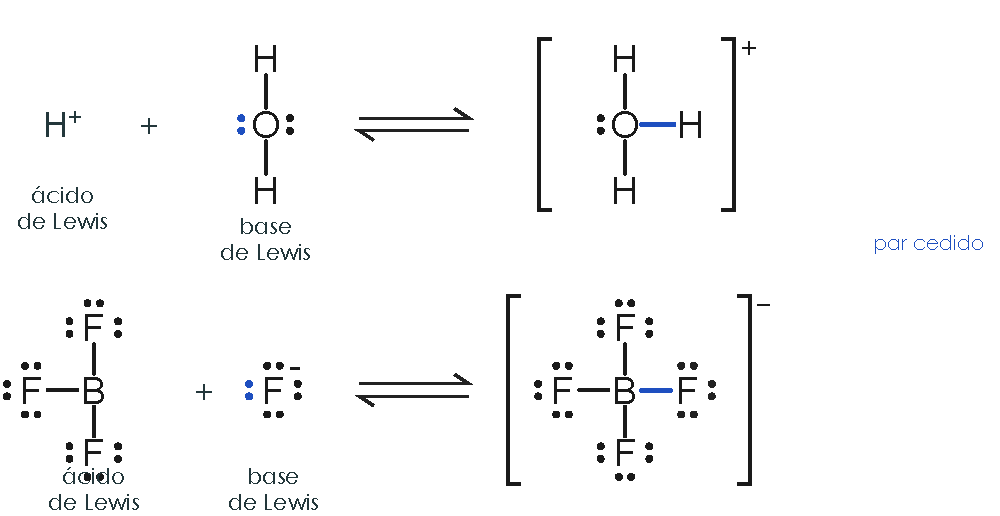
\includegraphics[width=0.7\linewidth]{FigurasSVG/UD7_Equilibrio_Acido_Base/pdf/UD7_01_acidos_bases_lewis.pdf}
    \caption{Ácidos y bases de Lewis}
    \label{fig:acidoybaselewis}
\end{figure}

% \begin{figure}[H]
%     \centering
%     \includegraphics[scale=.7]{lewis_teoria.png}
% \end{figure}


\section{Fortaleza de los ácidos y bases: constante de acidez y constante de basicidad}\label{sec:fortaleza-de-los-acidos-y-bases:-constante-de-acidez-y-constante-de-basicidad}

La disociación de un ácido o una base está gobernada, como todas las reacciones por su constante de equilibrio.
Por norma general se usa la constante de disociación o de acidez \(k_a\) para un ácido o la constante de basicidad \(k_b\) para una base donde ya está incluida la \conc{H2O} que se considera invariable.

Sea la reacción entre un ácido general \ch{HA} y \water.
\begin{centeredequation}
    \ch{!(ácido 1)(HA) + !(base 2)(H2O) <=> !(base 1)(A-) + !(ácido 2)(H3O+ )}
\end{centeredequation}


Su constante de equilibrio sería:

\begin{gather*}
    K = \dfrac{\conc{A-}\ \conc{H3O+}}{\conc{HA}\ \conc{H2O}}\separ
    k_a = k\conc{H2O} = \dfrac{\conc{A-}\ \conc{H3O+}}{\conc{HA}}
\end{gather*}

A mayor valor de la constante de acidez \(k_a\) mayor será la disociación y por tanto más fuerte será el ácido.

\begin{enumerate}[label=\numberballmDarkTeal]
        \item \negsubro{Ácidos fuertes}: están completamente disociados o casi completamente disociados en disolución diluida, es decir una concentración menor a\concentracion[m]{0.1}.
        En estos ácidos tenemos prácticamente la base conjugada (\ch{A-}) y no existen moléculas sin disociar (\ch{HA}), esto provoca que el valor de \(k_a\) sea muy alto (superior a \num{e3}) y se dice que el grado de disociación \(\bm{\alpha}\) es de prácticamente la unidad.
        En el caso de los ácidos fuertes no es necesario dar un valor de \Ka{} porque se considera al ácido completamente disociado quedando todo el ácido en sus correspondientes iones.
        \item \negsubro{Ácidos débiles}: no se disocian completamente en disolución diluida.
        Estas especies presentan simultáneamente las formas \ch{HA} y \ch{A-}.
        La proporción entre ambas especies vendrá dada por la correspondiente \Ka{}
\end{enumerate}
Debido a que algunas veces los valores de \Ka suelen ser muy pequeños y las potencias en base \num{10} no son muy manejables, se introduce una nueva magnitud llamada \pKa como:
\begin{centeredequation}
    pK_a = -\log K_a  \label{eq:pka}
\end{centeredequation}


Un tratamiento similar se puede hacer para las especies básicas.
% ? \marcador{poner ejercicios tipo página 206}

% ?\subsection{Relación entre la estructura de los ácidos y su fuerza}
% ? \marcador{duda por si poner esto}

\subsection{Fortaleza de los ácidos y bases conjugados}\label{subsec:fortaleza-de-los-acidos-y-bases-conjugados}

\begin{itemize}
    \item La base conjugada de un ácido fuerte, es una base débil.
    \item La base conjugada de un ácido débil, es una base fuerte.
    \item El ácido conjugado de una base fuerte, es un ácido débil.
    \item El ácido conjugado de una base débil, es un ácido fuerte.
\end{itemize}


\section{Medida de la acidez. pH}\label{sec:medida-de-la-acidez.-ph}

\subsection{Equilibrio de ionización del agua}\label{subsec:equilibrio-de-ionizacion-del-agua}

Anteriormente, se ha indicado que el agua es una especie anfótera que puede comportarse como ácido o como base según la sustancia con la que interactúe.
Esto permite que las moléculas de agua reaccionen entre ellas, actuando unas como ácidos y otras como bases:
\begin{centeredequation}
    \ch{!(ácido 1)(H2O) + !(base 2)(H2O) <=> !(base 1)(OH-) + !(ácido 2)(H3O+ )}
\end{centeredequation}

La constante de equilibrio sería por tanto:
\begin{centeredequation}
    \Kw = \dfrac{\conc{OH-}\ \conc{H3O+}}{\conc{H2O}\ \conc{H2O}}\label{eq:cte-agua-inicio}
\end{centeredequation}

Como hemos dicho anteriormente, la \conc{H2O} se puede considerar constante por lo que podemos escribir la constante de equilibrio del agua \Kw{} como:
\begin{centeredequation}
    \Kw = \conc{H3O+}\ \conc{OH-}\label{eq:cte-agua}
\end{centeredequation}


A esta \(k_w\) se le conoce como \negrita{producto iónico del agua}.
Su valor dependerá de la temperatura y a \temperatura[c]{25} es de:
\begin{centeredequation}
    \Kw = \num{e-14}
    \label{eq:valor-de-k-agua}
\end{centeredequation}


El bajo valor de \(k_w\) indica que el agua se encuentra muy poco disociada.

\begin{itemize}
    \item \negrita{En disoluciones neutras}: la \(\conc{H3O+} = \conc{OH-}\) siendo esta la condición de neutralidad sea cual sea la temperatura.
    A \temperatura[c]{25} tendremos que:
    \begin{gather*}
        \conc{H3O+} = \concentracion[m]{e-7}\separ
        \conc{OH-} = \concentracion[m]{e-7}
    \end{gather*}
    \item \negrita{En disoluciones ácidas}: \(\conc{H3O+} > \conc{OH-}\).
    Si disolvemos un ácido, este aportará iones oxonio \ch{H3O+} y disminuye por tanto la concentración de iones hidroxilo \ch{OH-}. A \temperatura[c]{25} tendremos que:
    \begin{gather*}
        \conc{H3O+} > \concentracion[m]{e-7}\separ
        \conc{OH-} < \concentracion[m]{e-7}
    \end{gather*}
    \item \negrita{En disoluciones básicas}: \(\conc{H3O+} < \conc{OH-}\).
    Si disolvemos una base, esta aportará iones hidroxilo disminuyendo así la concentración de iones oxonio.
    A \temperatura[c]{25} tendremos que:
    \begin{gather*}
        \conc{H3O+} < \concentracion[m]{e-7}\separ
        \conc{OH-} > \concentracion[m]{e-7}
    \end{gather*}
\end{itemize}

\subsection{Concepto y escala de pH}\label{subsec:concepto-y-escala-de-ph}

El químico danés \negrita{S\o{}ren Peter S\o{}rensen} introdujo en \num{1909} el concepto de \negrita{pH} para facilitar el manejo de las concentraciones de \ch{H3O+}.
Para expresar la concentración en forma de números sencillos, S\o{}rensen definió una escala logarítmica del modo que:
\begin{centeredequation}
    \pH = -\log\ \conc{H3O+}\label{eq:pH}
\end{centeredequation}


Si por ejemplo una disolución tiene \conc{H3O+} = \concentracion[m]{e-4}, entonces su pH será:
\begin{centeredequation}
    pH = -\log\ \conc{H3O+} = 4
\end{centeredequation}

De manera análoga podemos definir el pOH como:
\begin{centeredequation}
    \pOH = -\log\ \conc{OH-}\label{eq:pOH}
\end{centeredequation}

\begin{itemize}
    \item En las \negrita{disoluciones ácidas}, \(\conc{H3O+} > \concentracion[m]{e-7}\) y \(\conc{OH-} < \concentracion[m]{e-7}\) entonces tendremos que \(pH < 7\) y \(pOH > 7\).
    \item En las \negrita{disoluciones neutras}, \(\conc{H3O+} = \concentracion[m]{e-7}\) y \(\conc{OH-} = \concentracion[m]{e-7}\) entonces tendremos que \(pH = 7\) y \(pOH = 7\).
    \item En las \negrita{disoluciones básicas}, \(\conc{H3O+} < \concentracion[m]{e-7}\) y \(\conc{OH-} > \concentracion[m]{e-7}\) entonces tendremos que \(pH > 7\) y \(pOH < 7\).
\end{itemize}

A partir de la expresión del producto iónico del agua, a una temperatura de \temperatura[c]{25} tendremos que:
\begin{gather*}
    k_w = \conc{H3O+}\ \conc{OH-}\separ
    \num{e-14} = \conc{H3O+}\ \conc{OH-}
\end{gather*}

Si tomamos \(-\log\) de la última expresión tendríamos que:

\begin{gather*}
    -\log\ \num{e-14} =\underbrace{-\log\ \conc{H3O+}}_{\color{blue}\text{pH}} + \underbrace{-\log\ \conc{OH-}}_{\color{red}{\text{pOH}}} \separ
    14 = \text{pH} + \text{pOH}
\end{gather*}

Por lo tanto, podemos decir que en una disolución acuosa a \temperatura[c]{25} tendremos que:
\begin{centeredequation}
    \text{pH} + \text{pOH} = 14\label{eq:sumapHypOH}
\end{centeredequation}


\begin{figure}[H]
    \centering
    % [FIGURA ORIGINAL] \includegraphics[scale=.7]{images/imagesUD7EquilibrioAcidoBase/UD7_Teoria/escala_ph}
    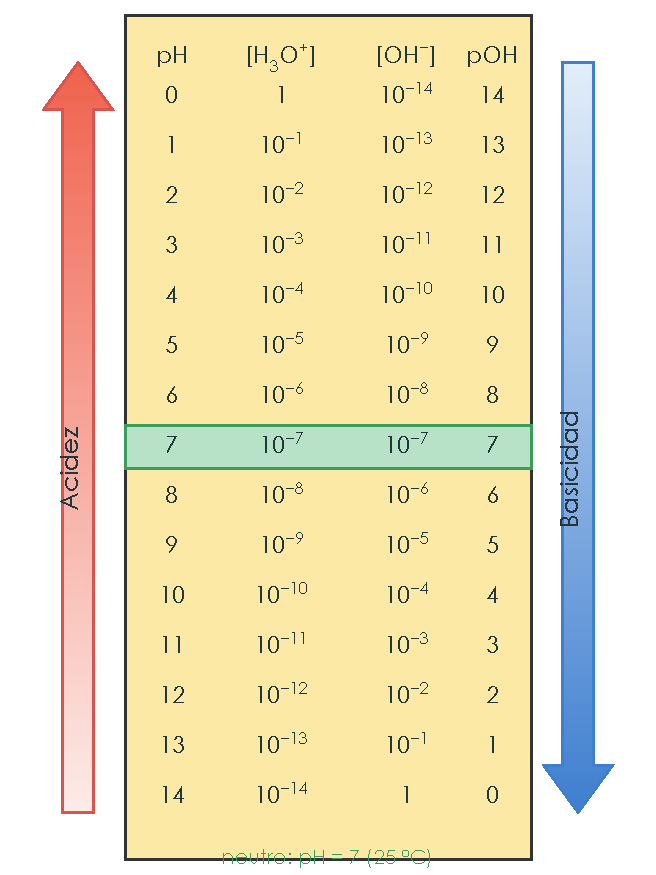
\includegraphics[width=0.5\linewidth]{FigurasSVG/UD7_Equilibrio_Acido_Base/pdf/UD7_02_escala_pH.pdf}
    \caption{Escala del pH y pOH junto con las concentraciones de \ch{H3O+} y \ch{OH-}}
    \label{fig:escala_ph}
\end{figure}


\section{Relación entre la constante de acidez de un ácido y la constante de basicidad de su base conjugada}

La constante de acidez de un ácido (\Ka) la podemos relacionar con la constante de basicidad de su base conjugada (\Kb) a partir de la constante \Kw según la expresión:
\begin{centeredequation}
    \Ka \cdot \Kb = \Kw
\end{centeredequation}

Si tomamos \( -\log \) en ambos términos y sabiendo que \( \Kw = \num{e-14} \) tendremos que:
\begin{centeredequation}
    \pKa + \pKb = 14
\end{centeredequation}


\section{Indicadores químicos}\label{sec:indicadores-quimicos}

Para detectar las variaciones de pH normalmente se han utilizado \negrita{sustancias indicadoras} llamados \negrita{Indicadores} que a partir de ahora se abreviarán como \azuln{HIn} (forma ácida) o \rojon{\ch{In-}} (forma básica).

Estos indicadores son ácidos o bases débiles que también experimentan un equilibrio pero tienen la peculiaridad de que tienen un color diferente en la forma ácida \negrita{\ch{HIn}} y en la forma básica \negrita{\negrita{\ch{In-}}} por lo que podemos escribir su correspondiente equilibrio y por tanto obtener su correspondiente constante de equilibrio que la representaremos como \(k_{\text{HIn}}\)

\begin{centeredequation}
    \ch{!( "\textcolor{red}{Color\ A}" )(\color{red}HIn) + H2O <=> !( "\textcolor{blue}{Color\ B}" )(\color{blue}In-) + H3O+}
\end{centeredequation}

\begin{centeredequation}
    k_{\text{HIn}} = \dfrac{\conc{In-}\ \conc{H3O+}}{\conc{HIn}}
\end{centeredequation}

Al tratarse de ácidos y/o bases débiles ambas especies estarán presentes en el equilibrio.
Para poder apreciar correctamente el cambio de color, la concentración de una de las especies debe ser al menos diez veces mayor que la concentración de la otra es decir:

\begin{itemize}
    \item \negrita{Color ácido}: para ver el color de la forma ácida necesitaremos que al menos \(\conc{HIn} = 10\ \conc{In-}\).
    \item \negrita{Color básico}: para ver el color de la forma básica necesitaremos que al menos \(\conc{In-} = 10\ \conc{HIn}\).
\end{itemize}

Según lo visto, el cambio de color no se producirá a un valor fijo de pH sino que se hará en un intervalo de pH que vendrá determinado por la \(k_{\text{HIn}}\).

Y ese intervalo será:
\begin{centeredequation}
    \text{pH} = \text{pk\subin{HIn}} \pm 1\label{eq:intervalo-indicar}
\end{centeredequation}

A este intervalo de pH en el que se produce el cambio de color se le denomina \negrita{intervalo de viraje}.


Para llegar a la ecuación \eqref{eq:intervalo-indicar} debemos hacerlo en dos partes, estableciendo dos condiciones que se detallan a continuación:

\begin{itemize}
    \item \textbf{Predomina el color de la forma ácida}, sería el \rojo{color A}. Si predomina el color de la forma ácida tendremos que \( \conc{HIn} = 10\ \conc{In-}  \).
    \begin{gather}
        K_{\ch{HIn}} = \dfrac{\conc{H3O+}\conc{In-}}{\conc{HIn}} \longrightarrow \conc{H3O+} = K_{\ch{HIn}} \cdot \dfrac{\conc{HIn}}{\conc{In-}} \notag \\[2mm]
        \text{tomamos } -\log \text{ en ambos términos}\notag \\[2mm]
        -\log{\conc{H3O+}} = -\log{\left( \dfrac{\conc{HIn}}{\conc{In-}} \right)} \notag \\[2mm]
        \pH = \text{pk\subin{HIn}}  -\log{\left( \dfrac{\conc{HIn}}{\conc{In-}} \right)} \notag \\[2mm]
        \pH = \text{pk\subin{HIn}}  -\log{\left( \dfrac{10\ \conc{In-}}{\conc{In-}} \right)} \notag \\[2mm]
        \pH = \text{pk\subin{HIn}}  -\log{10} \notag \\[2mm]
        \pH = \text{pk\subin{HIn}}  - 1 \label{eq:intervalo_ph_resta_1}
    \end{gather}
    \item \textbf{Predomina el color de la forma básica}, sería el \azul{color B}.
    Si predomina el color de la forma básica tendremos que \( \conc{In-} = 10\ \conc{HIn}  \).
    \begin{gather}
        K_{\ch{HIn}} = \dfrac{\conc{H3O+}\conc{In-}}{\conc{HIn}} \longrightarrow \conc{H3O+} = K_{\ch{HIn}} \cdot \dfrac{\conc{HIn}}{\conc{In-}} \notag \\[2mm]
        \text{tomamos } -\log \text{ en ambos términos}\notag \\[2mm]
        -\log{\conc{H3O+}} = -\log{\left( \dfrac{\conc{HIn}}{\conc{In-}} \right)} \notag \\[2mm]
        \pH = \text{pk\subin{HIn}}  -\log{\left( \dfrac{\conc{HIn}}{\conc{In-}} \right)} \notag \\[2mm]
        \pH = \text{pk\subin{HIn}}  -\log{\left( \dfrac{\conc{HIn}}{10\ \conc{HIn}} \right)} \notag \\[2mm]
        \pH = \text{pk\subin{HIn}}  -\log{\dfrac{1}{10}} \notag \\[2mm]
        \pH = \text{pk\subin{HIn}}  + 1 \label{eq:intervalo_ph_suma_1}
    \end{gather}
\end{itemize}

Si combinamos las ecuaciones \eqref{eq:intervalo_ph_suma_1} y la ecuación \eqref{eq:intervalo_ph_resta_1} tendremos la ecuación \eqref{eq:intervalo-indicar}


%\begin{ejemplo}
%    Demostrar matemáticamente que el intervalo de viraje de un indicador estará en un intervalo de \(\text{pH} = \text{pk\subin{HIn}} \pm 1\)
%\end{ejemplo}

\subsection{Elección del indicador}

Debido a que el intervalo de viraje depende del propio indicador, no todos los indicadores son válidos para todas las disoluciones.


El \negrita{indicador} apropiado será aquel que cambie de color en el intervalo de pH en el que se produzca la neutralización.

A continuación tenemos una tabla donde se indican los indicadores más comunes así como su intervalo de viraje y los colores de cada una de las formas.


\begin{figure}[H]
    \centering
    % [FIGURA ORIGINAL] \includegraphics[scale=.7]{images/imagesUD7EquilibrioAcidoBase/UD7_Teoria/indicadores}
    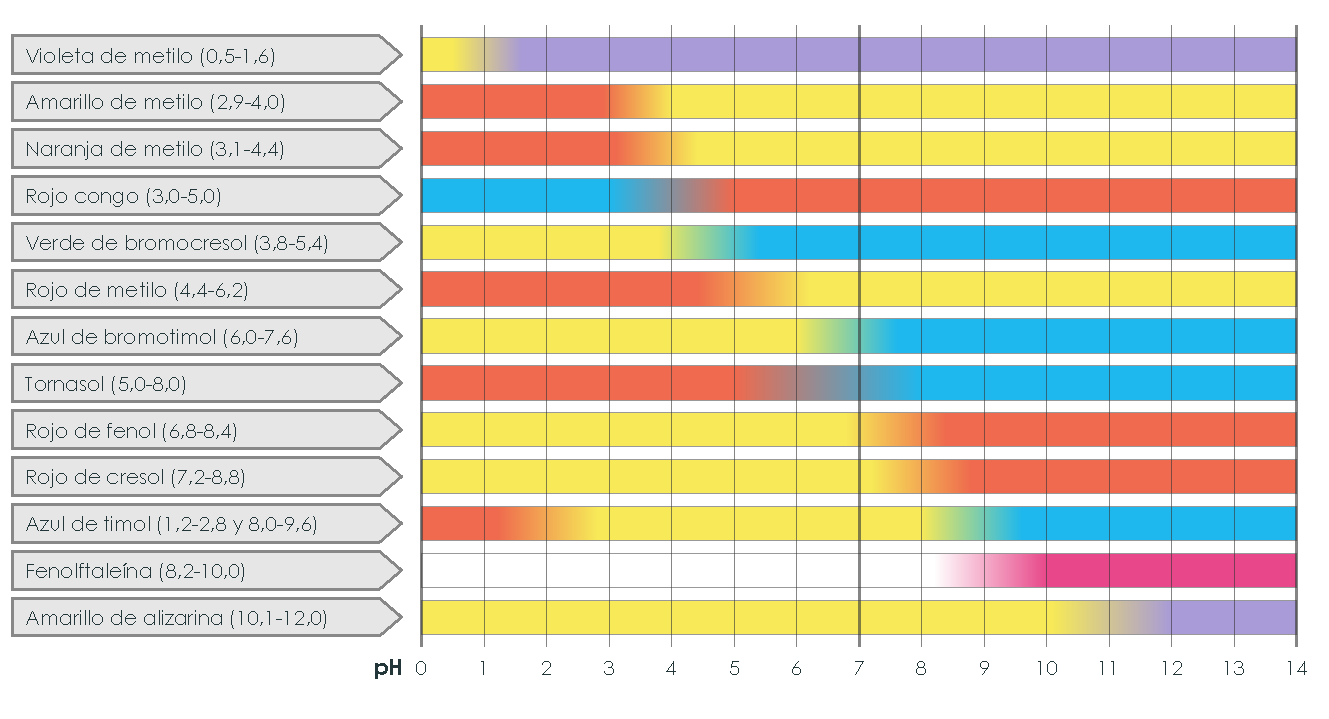
\includegraphics[width=0.95\linewidth]{FigurasSVG/UD7_Equilibrio_Acido_Base/pdf/UD7_03_indicadores.pdf}
    \caption{Colores de varios indicadores en función del pH}
    \label{fig:indicadores}
\end{figure}

%\section{Ácidos y bases poliionizables}\label{sec:acidos-y-bases-poliionizables}
%
%Existen ácidos y bases que pueden experimentar sucesivas ionizaciones (tantas disociaciones como número de hidrógenos que tenga) y cada una de ellas tendrán su correspondiente equilibrio y por tanto su correspondiente constante.
%
%Consideremos primero el ejemplo del ácido sulfúrico \ch{H2SO4}.
%La disociación de este ácido sería:
%
%\begin{gather*}
%    \ch{H2SO4 + H2O -> HSO4- + H3O+}; \separ
%    \ch{HSO4- + H2O <=> SO4^{2-} + H3O+}; \quad k_{a2} = \num{e-2}\separ
%\end{gather*}
%
%La primera disociación del sulfúrico, se considera que se encuentra totalmente disociado y, por tanto, no tiene sentido dar un valor de \Ka{}.
%El segundo equilibrio, si se considera un ácido débil y, por tanto, se da su correspondiente constante de equilibrio.
%
%Para el caso del ácido carbónico, ahora ambas disociaciones se consideran débiles y, por tanto, se dan dos constantes de acidez.
%
%\begin{table}[H]
%    \centering
%    \begin{tblr}{c}
%        \( \ch{H2CO3 + H2O <=> HCO3- + H3O+}; \quad k_{a1} = \num{4.3e-7}\)\\
%        \(\ch{HCO3- + H2O <=> CO3^{2-} + H3O+}; \quad k_{a2} = \num{5.61e-11}\)\\
%    \hline
%    \( \ch{H2CO3 + 2 H2O <=> CO3^{2-} + 2 H3O+}; \quad k = k_{a1}\cdot k_{a2}\)
%    \end{tblr}
%\end{table}


\section{Hidrólisis}\label{sec:hidrolisis}

\begin{center}
    \begin{definicion}[width=0.9\textwidth]{Hidrólisis}
        La \negrita{hidrólisis} es la reacción de los iones de una sal con el agua, que regenera un ácido o una base
    \end{definicion}
\end{center}


Para su tratamiento, tenemos que disociar primero la sal en sus correspondientes iones y luego llevar a cabo la reacción entre cada ion con el agua.

\subsection{Sal de ácido fuerte y base fuerte}\label{subsec:sal-de-acido-fuerte-y-base-fuerte}

Consideremos un ácido fuerte como \ch{HCl} y una base fuerte \ch{NaOH}.
Ambos reaccionan según la siguiente reacción produciendo \ch{NaCl} y agua:
\begin{centeredequation}
    \ch{HCl + NaOH -> NaCl + H2O}
\end{centeredequation}

La sal formada, por tanto, será el \ch{NaCl}, si disociamos esta sal tendremos:
\begin{centeredequation}
    \ch{NaCl -> Na+ + Cl-}
\end{centeredequation}


Como el \ch{Na+} es el ácido conjugado de una base fuerte, entonces será un ácido débil y \negrita{no} reaccionará con el agua.

Como el \ch{Cl-} es base conjugada de un ácido fuerte, entonces será una base débil y \negrita{no} reaccionará con el agua.

Podemos resumir entonces, que los ácidos y bases conjugadas procedentes de ácidos y bases fuertes no reaccionarán con el agua, es decir no se producirá hidrólisis de los mismos.

\caja{En este tipo de caso tendremos una disolución con \(\pH=7\) es decir una disolución \negrita{neutra}.}

\subsection{Sal de ácido débil y base fuerte}\label{subsec:sal-de-acido-debil-y-base-fuerte}

Consideremos ahora la reacción entre un ácido débil por ejemplo el ácido acético, que lo podemos esquematizar como \ch{HAc} y el hidróxido de potasio \ch{KOH} que es una base fuerte.
La reacción que tendrá lugar será:
\begin{centeredequation}
    \ch{HAc + KOH -> AcK + H2O}
\end{centeredequation}


Ahora, el acetato de potasio formado, lo podemos disociar en:
\begin{centeredequation}
    \ch{AcK -> Ac- + K+}
\end{centeredequation}


El ácido conjugado \ch{K+} al proceder de una base fuerte, no reaccionará con el agua puesto que es un ácido débil.
Ahora, la base conjugada acetato \ch{Ac-} es una base fuerte, puesto que procede de un ácido débil y por tanto si reaccionará con el agua según la reacción:
\begin{centeredequation}
    \ch{ Ac- + H2O <=> HAc + OH-}
\end{centeredequation}


Como vemos, se vuelve a formar el ácido conjugado del que procede y también iones hidroxilo.
La constante de este equilibrio y, en consecuencia, la constante de hidrólisis \Kh{} será.
\begin{centeredequation}
    \Kh = \dfrac{\conc{HAc}\ \conc{OH-}}{\conc{Ac-}} \label{eq:cte_hidrolisis_base}
\end{centeredequation}


\caja{En este tipo de caso tendremos una disolución con \(\text{pH}>7\) es decir una disolución \negrita{básica}.}

Esta constante de hidrólisis \Kh la podemos relacionar con la correspondiente constante de acidez del ácido conjugado \ch{HAc} y con el producto iónico del agua sabiendo que:
\begin{gather*}
    \ch{HAc + H2O <=> Ac- + H3O+}\separ
    \Ka = \dfrac{\conc{Ac-}\ \conc{H3O+}}{\conc{HAc}}
\end{gather*}

Si la expresión \eqref{eq:cte_hidrolisis_base} la multiplicamos y dividimos por la concentración de iones oxonio \ch{H3O+} tendremos que:
\begin{centeredequation}
    \Kh = \dfrac{{\color{blue}\conc{HAc}}\ {\color{red}\conc{OH-}}}{{\color{blue}\conc{Ac-}}}\dfrac{{\color{red}\conc{H3O+}}}{{\color{blue}\conc{H3O+}}}
\end{centeredequation}

como podemos ver:
\begin{centeredequation}
    \color{blue} \dfrac{1}{\Ka} = \dfrac{\conc{HAc}}{\conc{Ac-}\ \conc{H3O+}}
\end{centeredequation}

y que:
\begin{centeredequation}
    \color{red} \Kh = \conc{H3O+}\ \conc{OH-}
\end{centeredequation}

Por lo tanto, podemos decir que:
\begin{centeredequation}
    \Kh = \dfrac{{\color{red}\Kw}}{{\color{blue}\Ka}}
\end{centeredequation}


Esta \Kh hace referencia en este caso a la constante de equilibrio de la especie \ch{Ac-} por lo que la podemos escribir como K\textsubscript{\ch{Ac-}} y como el acetato es una base también la podemos escribir como \Kb

\subsection{Sal de ácido fuerte y base débil}\label{subsec:sal-de-acido-fuerte-y-base-debil}

Consideremos ahora el caso entre la reacción entre un ácido fuerte \ch{HCl} y una base débil como el amoniaco \ch{NH3}.
Ambas especies darán lugar a la siguiente reacción:
\begin{centeredequation}
    \ch{HCl + NH3 -> NH4Cl + H2O}
\end{centeredequation}

Ahora el cloruro de amonio formado lo podemos disociar en:
\begin{centeredequation}
    \ch{NH4Cl -> NH4+ + Cl-}
\end{centeredequation}


El ion \ch{Cl-} es una base débil, ya que proviene de un ácido fuerte y, por tanto, no reaccionará con el agua.
El \ch{NH4+} es un ácido fuerte, ya que proviene de una base débil y, por tanto, si reaccionará con el agua según la reacción:
\begin{centeredequation}
    \ch{NH4+ + H2O  <=> NH3 + H3O+}
\end{centeredequation}

En este caso, la constante de hidrólisis será:
\begin{centeredequation}
    \Kh = \dfrac{\conc{NH3}\ \conc{H3O+}}{\conc{NH4+}} \label{eq:cte_hidrolisis_acido}
\end{centeredequation}


\caja{En este tipo de casos tendremos una disolución de \(\text{pH}<7\) es decir una disolución \negrita{ácida}.}


De manera análoga al caso anterior, podemos relacionar la constante de hidrólisis con la constante de basicidad de la base formada en la hidrólisis, siendo en este caso el \ch{NH3}.

Si la expresión \eqref{eq:cte_hidrolisis_acido} la multiplicamos y dividimos por la concentración de iones oxonio \ch{OH-} tendremos que:
\begin{centeredequation}
    \Kh = \dfrac{{\color{blue}\conc{NH3}}\ {\color{red}\conc{H3O+}}}{{\color{blue}\conc{NH4+}}}\dfrac{{\color{red}\conc{OH-}}}{{\color{blue}\conc{OH-}}}
\end{centeredequation}

como podemos ver:
\begin{centeredequation}
    \color{blue} \dfrac{1}{k_a} = \dfrac{\conc{NH3}}{\conc{NH4+}\ \conc{OH-}}
\end{centeredequation}

y que:
\begin{centeredequation}
    \color{red} \Kh = \conc{H3O+}\ \conc{OH-}
\end{centeredequation}


Por lo tanto, podemos decir que:
\begin{centeredequation}
    \Kh = \dfrac{{\color{red}\Kw}}{{\color{blue}\Kb}}
\end{centeredequation}


Esta \Kh hace referencia en este caso a la constante de equilibrio de la especie \ch{NH4+} por lo que la podemos escribir como K\textsubscript{\ch{NH4+}} y como el amonio es un ácido también la podemos escribir como \Ka

\subsection{Sal de ácido débil y base débil}\label{subsec:sal-de-acido-debil-y-base-debil}

Imaginemos ahora la reacción entre ácido acético \ch{HAc} y \ch{NH3}.
\begin{centeredequation}
    \ch{HAc + NH3 -> AcNH4}
\end{centeredequation}


La sal formada \ch{AcNH4} se disociará según:
\begin{centeredequation}
    \ch{AcNH4 -> Ac- + NH4+}
\end{centeredequation}


En este caso, ambas especies reaccionarán con el agua al proceder de ácidos y bases débiles, teniendo entonces que:
\begin{centeredequation}
    \begin{aligned}
        \ch{NH4+ + H2O & <=> NH3 + H3O+}\separ
        \ch{ Ac- + H2O & <=> HAc + OH-}\separ
        \midrule
        \ch{NH4+ + Ac- +} \cancelred{\ch{2 H2O}} & <=> \ch{NH3 + HAc +} \cancelred{\ch{OH- + H3O+}}
    \end{aligned}
\end{centeredequation}

En este caso, la constante de hidrólisis quedaría como:
\begin{centeredequation}
    \Kh = \dfrac{\conc{NH3}\ \conc{HAc}}{\conc{NH4+}\ \conc{Ac-}} \label{eq:cte_hidrolisis_acido_base}
\end{centeredequation}

Si ahora la expresión \eqref{eq:cte_hidrolisis_acido_base} la multiplicamos y dividimos por \conc{H3O+} \conc{OH-} tendremos que:
\begin{centeredequation}
    \Kh = \dfrac{{\color{red}\Kw}}{{\color{blue}\Ka \cdot \Kb}}
\end{centeredequation}

\caja{En este caso, el valor del \pH{} dependerá de la fortaleza de cada especie, si \(\Ka>\Kb\) entonces la disolución será ácida y si \( \Ka < \Kb \) entonces la disolución será básica.}


\section{Disoluciones tampón}\label{sec:disoluciones-tampon}

Las disoluciones tampón también se llaman disoluciones \negrita{buffers}, \negrita{reguladoras} o \negrita{amortiguadoras} y son disoluciones que permiten mantener sin variar el pH de la disolución tras añadir un ácido o una base.

¿Cómo lo consiguen?
Estas disoluciones absorben un exceso de iones hidroxilo o un exceso de iones oxonio.

Estas disoluciones pueden ser de dos tipos:
\begin{enumerate}[label=\numberballmDarkTeal]
        \item \negsubro{Ácido débil y su sal}.
        Por ejemplo la mezcla entre \ch{CH3COOH + CH3COONa}.

        Cuando tenemos estas mezclas tendremos, por tanto, el siguiente equilibrio:
\begin{centeredequation}
    \ch{CH3COOH + H2O <=> CH3COO- + H3O+}
\end{centeredequation}


        Si escribimos la ecuación de la constante de equilibrio del \ch{CH3COOH}, despejamos la concentración de oxonio y luego tomamos \( -\log  \) en ambos términos tendremos una expresión que nos permite calcular el \pH{} de esa disolución reguladora:

%        Para calcular el pH de esta disolución reguladora se realiza según la expresión:
%        \begin{equation*}
%            \pH = \pKa + \log\dfrac{\conc{Sal}}{\conc{Ácido}}
%        \end{equation*}

%        En este caso tendríamos que:

        \begin{centeredequation}
            \pH = \pKa + \log\dfrac{\conc{CH3COO-}}{\conc{CH3COOH}}
        \end{centeredequation}

        En esta expresión, las cantidades disociadas se desprecian, puesto que son muy pequeñas comparadas con las cantidades de sal y de ácido que se añaden, simplificando así los cálculos.

        Al añadir una base, los iones hidroxilo reaccionan con el acético neutralizándose.
        De esta manera se evita que la disolución se vuelva básica.
        \begin{centeredequation}
            \ch{CH3COOH + OH- -> CH3COO- + H2O}
        \end{centeredequation}
        Cuando se añade un ácido, los iones oxonio se retiran de la disolución combinándose con \ch{CH3COO-} evitando así que la disolución se vuelva ácida.
        \begin{centeredequation}
            \ch{CH3COO- + H3O+ -> CH3COOH + H2O}
        \end{centeredequation}
        \item \negsubro{Base débil y su sal}.
        Por ejemplo la mezcla entre \ch{NH3 + NH4Cl}.

        Cuando tenemos estas mezclas tendremos, por tanto, el siguiente equilibrio:

        \begin{centeredequation}
            \ch{NH3 + H2O <=> NH4+ + OH-}
        \end{centeredequation}

        Para calcular el pH de esta disolución reguladora se calcula primero el \pOH{} según la expresión:
        \begin{centeredequation}
            \pOH = \pKb + \log\dfrac{\conc{Sal}}{\conc{Base}}
        \end{centeredequation}

        En este caso tendríamos que:

        \begin{centeredequation}
            \pOH = \pKb + \log\dfrac{\conc{NH4+}}{\conc{NH3}}
        \end{centeredequation}

        Una vez calculado el \pOH{} calculamos el \pH{} según:

        \begin{centeredequation}
            \pH + \pOH = 14
        \end{centeredequation}

        Al añadir una base, los iones hidroxilo reaccionan con el amonio neutralizándose evitando así que la disolución se vuelva básica.
        \begin{centeredequation}
            \ch{NH4+ + OH- -> NH3 + H2O}
        \end{centeredequation}
        Cuando se añade un ácido, los iones oxonio se retiran de la disolución combinándose con \ch{NH3} evitando así que la disolución se vuelva ácida.
        \begin{centeredequation}
            \ch{NH3 + H3O+ -> NH4+ + H2O}
        \end{centeredequation}
\end{enumerate}

% \begin{problemas}
%     \problema{. 86}. 
%     % Si se tienen \volumen[ml]{100} de una disolución de ácido etanoico \concentracion[m]{0.2}, ¿con cuál de las siguientes disoluciones lo mezclarías para formar la mejor disolución tampón posible?
%     % \begin{enumerate}[label=\letraminuscula]
%     %     \item \volumen[ml]{100} de disolución de \ch{CH3COONa} a \concentracion[m]{0.1}.
%     %     \item \volumen[ml]{100} de disolución de \ch{NaOH} a \concentracion[m]{0.1}.
%     %     \item \volumen[ml]{200} de disolución de \ch{CH3COONa} a \concentracion[m]{0.1}.
%     %     \item \volumen[ml]{100} de disolución de \ch{NaOH} a \concentracion[m]{0.2}.
%     % \end{enumerate}

%     \problema{. 96} 

%     \problema{. 105}. ¿Cuál es la variación en el \pH característico de una disolución reguladora que es \concentracion[m]{0.1} en ácido acético y 0,1 M en acetato de sodio, cuando a 1 L de la misma se le añaden 0,005 moles de  \ch{HCl}? Se desprecia la variación de volumen. 
% \end{problemas}


\section{Valoraciones ácido-base}\label{sec:valoraciones-acido-base}

Para determinar la concentración de una disolución de un ácido o una base se recurre a neutralizarla con otra disolución (base o ácido respectivamente) cuya concentración es conocida obteniéndose la concentración de la disolución desconocida a partir de las cantidades gastadas de una y de otra.

A este procedimiento se le denomina \negrita{volumetría ácido-base}.

Cuando ha reaccionado todo el ácido con toda la base, decimos que hemos llegado al \negrita{punto de equivalencia}

\subsection{Procedimiento operativo}\label{subsec:procedimiento-operativo}

Un procedimiento general sería:
\begin{itemize}
    \item Medir con exactitud un volumen de la disolución de concentración desconocida con una pipeta y ponerlo en un matraz Erlenmeyer.
    \item Verter en una bureta, la disolución de concentración conocida.
    \item Añadir 1 ó 2 gotas de un indicador químico a la disolución de concentración desconocida que tenemos en el matraz Erlenmeyer.
    \item Añadir gota a gota desde la bureta hasta el matraz Erlenmeyer removiendo la disolución desconocida durante la adición.
    Se recomienda poner un papel blanco debajo del Erlenmeyer para visualizar mejor el cambio de color.
    \item Cuando se produce el cambio de color del indicador, leer el volumen gastado en la bureta.
\end{itemize}

\subsection{Cálculos estequiométricos}\label{subsec:calculos-estequiometricos}

Al llegar a la neutralización, los moles de \ch{H3O+} y los moles de \ch{OH-} que han reaccionado tienen que ser los mismos.
Podemos realizar los cálculos de varias maneras:

\negsubro{Método 1}:

\begin{enumerate}[label=\numberballmDarkTeal]
        \item Escribiendo la reacción ajustada que tiene lugar y llevar a cabo los cálculos estequiométricos.
        \item Si nos dan los datos de concentración molar y volumen podremos, escribir la reacción ajustada que tiene lugar y aplicar la fórmula:

        \begin{centeredequation}
            n_{\text{ácido}}\cdot M_{\text{ácido}}\cdot V_{\text{ácido}} = n_{\text{base}}\cdot M_{\text{Base}}\cdot V_{\text{Base}}\label{eq:valoracion-acido-base-ecuacion}
        \end{centeredequation}

        Siendo \(n_{\text{base}}\) el coeficiente estequiométrico de la base, \(n_{\text{ácido}}\) el coeficiente estequiométrico del ácido y \(M_{\text{ácido}}\) y \(M_{\text{Base}}\) las concentraciones molares del ácido y de la base, respectivamente.
\end{enumerate}

\negsubro{Método 2}:

\begin{enumerate}[label=\numberballmDarkTeal]
        \item Utilizando la Normalidad y la ecuación:

        \begin{centeredequation}
            \text{nº eq-g ácido} =  \text{nº eq-g base}
        \end{centeredequation}

        Esta última expresión lo podemos poner en función de la normalidad y del volumen según:

        \begin{centeredequation}
            N_{\text{ácido}}\cdot V_{\text{ácido}} =  N_{\text{Base}}\cdot V_{\text{Base}}
        \end{centeredequation}

        Si lo que queremos es una expresión, en la que se tenga la molaridad, sabiendo que \(N = M \cdot \text{valencia}\) tendremos que:

        \begin{centeredequation}
            \text{valencia\subin{ácido}}\cdot M_{\text{ácido}}\cdot V_{\text{ácido}} = \text{valencia\subin{base}}\cdot M_{\text{Base}}\cdot V_{\text{Base}}
        \end{centeredequation}

\end{enumerate}

\negsubro{RECORDATORIO}:

\begin{centeredequation}
    N = \dfrac{n^\text{º}\ eq-g}{\text{V(L)}}; \qquad n^\text{º}\ eq-g = \dfrac{m(g)}{P_{eq}} \qquad P_{eq} = \dfrac{M_w}{Valencia}
\end{centeredequation}

Siendo \(n^\text{º}\ eq-g\) el número de equivalentes gramo de dicha especie, \(P_{eq}\) es el peso equivalente, \(M_w\) es la masa molecular.

Para calcular la valencia en los equilibrios ácido-base, podemos seguir la siguiente regla.

\begin{itemize}
    \item \negrita{Ácidos}: Será el número de hidrógenos que se transfiera en la reacción.
    \item \negrita{Bases}: Será el número de iones hidroxilo que tenga dicha especie.
    En el caso de no tener grupos hidroxilo como es el caso del amoniaco, será el número de hidrones que pueda aceptar.
\end{itemize}

\subsection{Curvas de valoración}\label{subsec:curvas-de-valoracion}

Una curva de valoración es la representación del pH frente al volumen de agente valorante.
Dependiendo de la naturaleza de cada reactivo, la curva de valoración será diferente.
\begin{enumerate}[label=\numberballmDarkTeal]
        \item \negsubro{Ácido débil - Base fuerte}: el punto de equivalencia se encuentra en un intervalo no muy grande en un pH ligeramente básico.
        Siendo su gráfica:

        \begin{figure}[H]
            \centering
            % [FIGURA ORIGINAL] \includegraphics[scale=0.7]{images/imagesUD7EquilibrioAcidoBase/UD7_Teoria/acido_debil_base_fuerte}\label{fig:acidodebil-base-fuerte}
            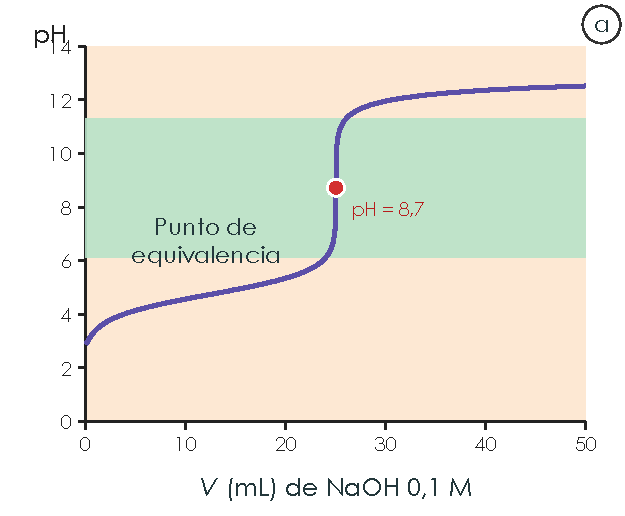
\includegraphics[width=0.55\linewidth]{FigurasSVG/UD7_Equilibrio_Acido_Base/pdf/UD7_04_valoracion_acido_debil_base_fuerte.pdf}\label{fig:acidodebil-base-fuerte}
        \end{figure}

        \item \negsubro{Base débil - Ácido fuerte}: muy parecido al caso anterior, pero en este caso el intervalo de viraje en el pH será ligeramente ácido.

        \begin{figure}[H]
            \centering
            % [FIGURA ORIGINAL] \includegraphics[scale=0.7]{images/imagesUD7EquilibrioAcidoBase/UD7_Teoria/base_debel_acido_fuerte}\label{fig:basedebil-acido-fuerte}
            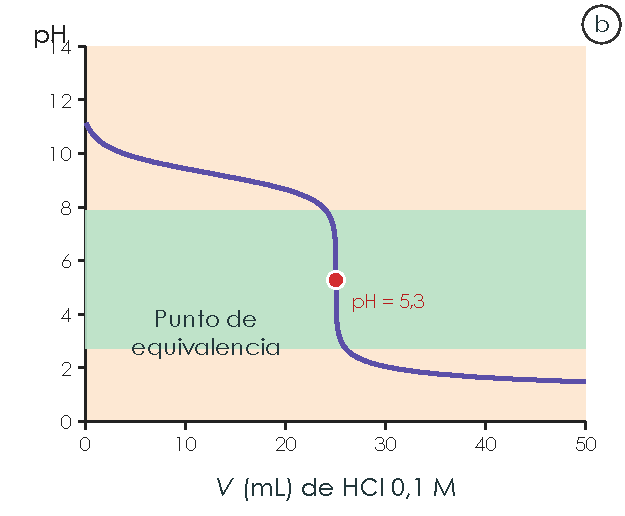
\includegraphics[width=0.55\linewidth]{FigurasSVG/UD7_Equilibrio_Acido_Base/pdf/UD7_05_valoracion_base_debil_acido_fuerte.pdf}\label{fig:basedebil-acido-fuerte}
        \end{figure}

        \item \negsubro{Ácido fuerte - Base fuerte}: el intervalo del pH en el punto de equivalencia es muy grande lo que permite usar muchos indicadores.

        \begin{figure}[H]
            \centering
            % [FIGURA ORIGINAL] \includegraphics[scale=0.7]{images/imagesUD7EquilibrioAcidoBase/UD7_Teoria/acido_fuerte_base_fuerte}\label{fig:acidofuerte-base-fuerte}
            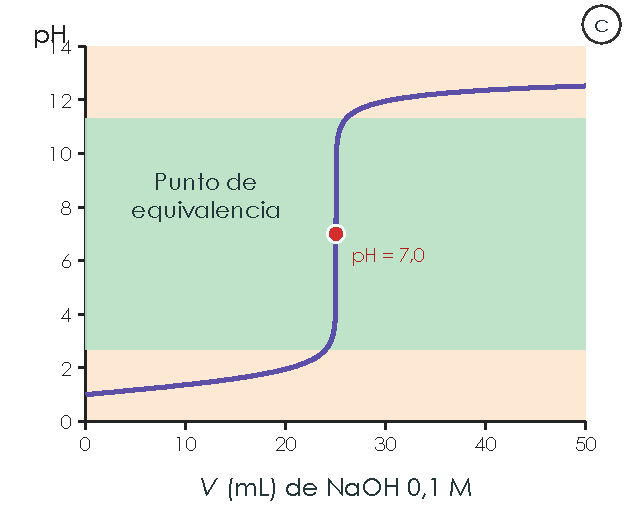
\includegraphics[width=0.55\linewidth]{FigurasSVG/UD7_Equilibrio_Acido_Base/pdf/UD7_06_valoracion_acido_fuerte_base_fuerte.pdf}\label{fig:acidofuerte-base-fuerte}
        \end{figure}

        \item \negsubro{Ácido débil - Base débil}: el intervalo en el pH en el punto de equivalencia es muy estrecho lo que resulta muy difícil su determinación.

        \begin{figure}[H]
            \centering
            % [FIGURA ORIGINAL] \includegraphics[scale=.7]{images/imagesUD7EquilibrioAcidoBase/UD7_Teoria/acido_debil_base_debil}\label{fig:acido-debil-base-debil}
            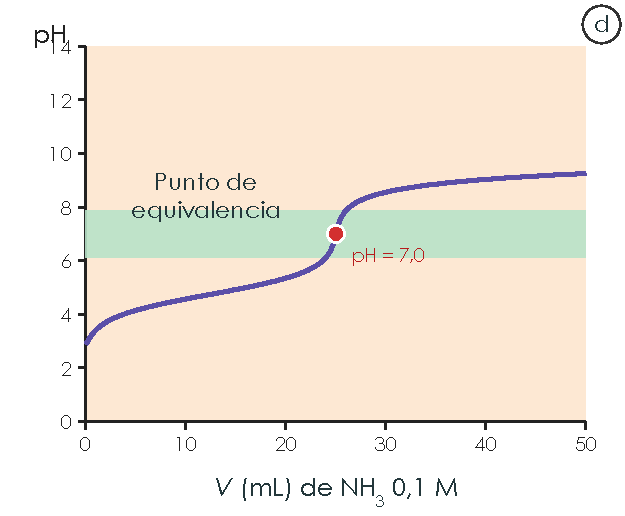
\includegraphics[width=0.55\linewidth]{FigurasSVG/UD7_Equilibrio_Acido_Base/pdf/UD7_07_valoracion_acido_debil_base_debil.pdf}\label{fig:acido-debil-base-debil}
        \end{figure}

\end{enumerate}




    \newpage

    %! Author = Profesor
%! Date = 06/06/2024


\section{Ejercicios}

\subsection{Ejercicios}

\begin{exercise}
    Se dispone de\ch{NaOH} con impurezas de \ch{Ca(OH)2}. Una muestra de \masa[g]{0.77} de esta mezcla se disuelve en agua hasta obtener \SI{100}{\cubic\centi\metre} de disolución. \SI{10}{\cubic\centi\metre} de disolución necesitan \SI{20}{\cubic\centi\metre} de HCl \concentracion[m]{0.1} para su neutralización.
    Calcula el \% en peso de NaOH en la muestra.

    \begin{solu}
%        \begin{figure}[H]
%            \centering
%            \includegraphics[scale=.5]{images/imagesUD7EquilibrioAcidoBase/UD7_Problemas/general_01}
%            %\caption{}
%            %\label{fig:}
%        \end{figure}

        Sean \(x\) los moles de \ch{NaOH} e \(y\) los moles de \ch{Ca(OH)2} presentes en los \SI{100}{\centi\metre\cubed} de disolución.

        En \SI{10}{\centi\metre\cubed} (una décima parte de la muestra) hay \(x/10\) mol de \ch{NaOH} e \(y/10\) mol de \ch{Ca(OH)2}. Los moles de \ch{HCl} empleados en la neutralización son:

        \begin{equation*}
            n(\ch{HCl}) = 0,020 \ \si{\litre} \times 0,1 \ \si{\Molar} = \num{2e-3} \ \text{mol}
        \end{equation*}

        Como cada mol de \ch{NaOH} neutraliza 1 mol de \ch{HCl} y cada mol de \ch{Ca(OH)2} neutraliza 2 mol de \ch{HCl}:

        \begin{equation*}
            \dfrac{x}{10} + 2\, \dfrac{y}{10} = 2 \times 10^{-3} \ \Rightarrow \ x + 2y = 0,02 \qquad \text{(i)}
        \end{equation*}

        Además, la masa total de la muestra es (\(M(\ch{NaOH}) = 40\), \(M(\ch{Ca(OH)2}) = 74\)):

        \begin{equation*}
            40 x + 74 y = 0,77 \qquad \text{(ii)}
        \end{equation*}

        De (i): \(x = 0,02 - 2y\). Sustituyendo en (ii):

        \begin{equation*}
            40(0,02-2y) + 74y = 0,77 \ \Rightarrow \ 0,8 - 80y + 74y = 0,77 \ \Rightarrow \ -6y = -0,03 \ \Rightarrow \ y = 0,005 \ \text{mol}
        \end{equation*}

        \begin{equation*}
            x = 0,02 - 2(0,005) = 0,01 \ \text{mol de \ch{NaOH}}
        \end{equation*}

        La masa de \ch{NaOH} en la muestra es \(m = 0,01 \times 40 = \SI{0.4}{\gram}\), por lo que el porcentaje en peso de \ch{NaOH} es:

        \begin{equation*}
            \%\, \ch{NaOH} = \dfrac{0,4}{0,77} \times 100 = 51,9\ \%
        \end{equation*}

    \end{solu}
\end{exercise}

\begin{exercise}
    La densidad de un vinagre comercial (5 \% en peso de \chemfig{CH_3COOH} es de \densidad[gml]{1.0055}. Expresa la concentración del soluto en molaridad y fracción molar. ¿Qué volumen de hidróxido sódico \concentracion[m]{0.5} se necesitará para neutralizar \volumen[ml]{250} del mencionado vinagre?
    \begin{solu}
%        \begin{figure}[H]
%            \centering
%            \includegraphics[scale=.5]{images/imagesUD7EquilibrioAcidoBase/UD7_Problemas/general_02}
%            %\caption{}
%            %\label{fig:}
%        \end{figure}

        Tomamos como base de cálculo 1 L de disolución. La masa de esta disolución es:

        \begin{equation*}
            m = 1000 \ \si{\milli\litre} \times 1,0055 \ \si{\gram\per\milli\litre} = \SI{1005.5}{\gram}
        \end{equation*}

        La masa de ácido acético (5\,\% en peso) y de agua son:

        \begin{equation*}
            m(\ch{CH3COOH}) = 0,05 \times 1005,5 = \SI{50.28}{\gram} \qquad m(\ch{H2O}) = 1005,5 - 50,28 = \SI{955.22}{\gram}
        \end{equation*}

        \textbf{Molaridad}

        Con \(M(\ch{CH3COOH}) = \SI{60}{\gram\per\mole}\):

        \begin{equation*}
            n(\ch{CH3COOH}) = \dfrac{50,28}{60} = 0,838 \ \text{mol} \ \Rightarrow \ [\ch{CH3COOH}] = \SI{0.838}{\Molar}
        \end{equation*}

        \textbf{Fracción molar}

        Con \(M(\ch{H2O}) = \SI{18}{\gram\per\mole}\):

        \begin{equation*}
            n(\ch{H2O}) = \dfrac{955,22}{18} = 53,07 \ \text{mol}
        \end{equation*}

        \begin{equation*}
            x_{\ch{CH3COOH}} = \dfrac{0,838}{0,838+53,07} = 0,0155
        \end{equation*}

        \textbf{Volumen de \ch{NaOH} 0,5 M necesario}

        La reacción de neutralización es \(\ch{CH3COOH + NaOH -> CH3COONa + H2O}\) (1:1). Los moles de ácido en \volumen[ml]{250} de vinagre son:

        \begin{equation*}
            n(\ch{CH3COOH}) = 0,838 \ \si{\Molar} \times 0,250 \ \si{\litre} = 0,2095 \ \text{mol}
        \end{equation*}

        \begin{equation*}
            V(\ch{NaOH}) = \dfrac{0,2095}{0,5} = 0,419 \ \si{\litre} = \SI{418.9}{\milli\litre}
        \end{equation*}

    \end{solu}
\end{exercise}

\begin{exercise}
    Se mezclan \volumen[ml]{75} de una disolución de \ch{HCl} \concentracion[m]{0.2} con \volumen[ml]{50} de otra solución también de \ch{HCl} pero \concentracion[m]{0.5}. Con la disolución resultante se valoran \volumen[ml]{20} de una solución de \ch{NaOH}, empleándose \volumen[ml]{25}. ¿Cuál es la molaridad de la solución de hidróxido sódico?
    \begin{solu}
%        \begin{figure}[H]
%            \centering
%            \includegraphics[scale=.5]{images/imagesUD7EquilibrioAcidoBase/UD7_Problemas/general_03}
%            %\caption{}
%            %\label{fig:}
%        \end{figure}

        Al mezclar las dos disoluciones de \ch{HCl}, los moles totales de \ch{HCl} son:

        \begin{equation*}
            n(\ch{HCl}) = 0,075 \times 0,2 + 0,050 \times 0,5 = 0,015 + 0,025 = 0,04 \ \text{mol}
        \end{equation*}

        El volumen total de la mezcla es \(75+50 = \SI{125}{\milli\litre}\), por lo que:

        \begin{equation*}
            [\ch{HCl}] = \dfrac{0,04}{0,125} = \SI{0.32}{\Molar}
        \end{equation*}

        Al valorar \volumen[ml]{20} de esta disolución (\(\ch{HCl}\) es un ácido fuerte, totalmente disociado), los moles de \ch{H3O+} (y de \ch{HCl}) son:

        \begin{equation*}
            n(\ch{HCl}) = 0,32 \times 0,020 = \num{6.4e-3} \ \text{mol}
        \end{equation*}

        Como la reacción de neutralización \(\ch{HCl + NaOH -> NaCl + H2O}\) es 1:1, estos moles deben coincidir con los moles de \ch{NaOH} empleados (\volumen[ml]{25}):

        \begin{equation*}
            [\ch{NaOH}] = \dfrac{6,4 \times 10^{-3}}{0,025} = \SI{0.256}{\Molar}
        \end{equation*}

    \end{solu}
\end{exercise}

\begin{exercise}
    El \ch{CaCO3} reacciona con una disolución de \ch{HNO3}, obteniéndose \ch{CO2}, \ch{Ca(NO3)2} y \ch{H2O}. Escribe el proceso que tiene lugar. ¿Qué volumen de \ch{CO2}, medido en condiciones normales, se formará por reacción de \volumen[ml]{60} de \ch{HNO3} \concentracion[m]{2.5} con exceso de \ch{CaCO3}? ¿Qué volumen de ácido nítrico comercial, del 64\% en peso y \densidad[gml]{1.4}  de densidad, se debe tomar para preparar los \volumen[ml]{60} \concentracion[m]{2.5} a los que se refiere el apartado anterior?
    \begin{solu}
%        \begin{figure}[H]
%            \centering
%            \includegraphics[scale=.5]{images/imagesUD7EquilibrioAcidoBase/UD7_Problemas/general_04}
%            %\caption{}
%            %\label{fig:}
%        \end{figure}

        La reacción ajustada es:

        \begin{equation*}
            \ch{CaCO3 \sld{} + 2 HNO3 \aq{} -> CO2 \gas{} + Ca(NO3)2 \aq{} + H2O \lqd{}}
        \end{equation*}

        \textbf{Volumen de \ch{CO2} en condiciones normales}

        Los moles de \ch{HNO3} son:

        \begin{equation*}
            n(\ch{HNO3}) = 0,060 \ \si{\litre} \times 2,5 \ \si{\Molar} = 0,15 \ \text{mol}
        \end{equation*}

        Como la estequiometría es 2 mol de \ch{HNO3} por cada mol de \ch{CO2} formado:

        \begin{equation*}
            n(\ch{CO2}) = \dfrac{0,15}{2} = 0,075 \ \text{mol}
        \end{equation*}

        En condiciones normales (0 ºC, 1 atm), el volumen molar es \SI{22.4}{\litre\per\mole}:

        \begin{equation*}
            V(\ch{CO2}) = 0,075 \times 22,4 = \SI{1.68}{\litre}
        \end{equation*}

        \textbf{Volumen de ácido nítrico comercial necesario}

        La masa de \ch{HNO3} puro necesaria (\(M(\ch{HNO3}) = \SI{63}{\gram\per\mole}\)) es:

        \begin{equation*}
            m(\ch{HNO3}) = 0,15 \times 63 = \SI{9.45}{\gram}
        \end{equation*}

        Como el ácido comercial tiene una riqueza del 64\,\% en peso:

        \begin{equation*}
            m_{disolución} = \dfrac{9,45}{0,64} = \SI{14.77}{\gram}
        \end{equation*}

        Y, con \(\rho = \SI{1.4}{\gram\per\milli\litre}\):

        \begin{equation*}
            V = \dfrac{14,77}{1,4} = \SI{10.55}{\milli\litre}
        \end{equation*}

    \end{solu}
\end{exercise}

\subsection{Ejercicios PAU}
\begin{exerciseEVAU}
Una disolución acuosa 0,3 M de ácido hipocloroso (HClO) tiene un pH de 3,98. Calcule:
  \begin{enumerate}[label=\letraminuscula]
      \item La concentración molar de todas las especies presentes en equilibrio.
      \item El grado de disociación del ácido hipocloroso.
      \item El valor de la constante de acidez (\Ka) del ácido hipocloroso y el valor de la constante de
basicidad (\Kb) de su base conjugada.
  \end{enumerate}
\begin{solu}

\end{solu}
\end{exerciseEVAU}

\begin{exerciseEVAU}
    En una planta de tratamiento de aguas se utiliza una disolución de hidróxido sódico (NaOH) para neutralizar
contaminantes ácidos. Para ajustar el pH antes del vertido, se añade ácido nítrico (HNO3) de concentración
conocida. Se dispone de 75 mL de una disolución de NaOH 0,20 M, a la que se añade HNO3 0,10 M.
Se supone que los volúmenes son aditivos. Calcule:
\begin{enumerate}[label=\letraminuscula]
    \item El pH cuando se han añadido 50 mL de \ch{HNO3}.
    \item Escriba la reacción de neutralización. Calcule el volumen de HNO3 necesario para alcanzar el
punto de equivalencia y el pH en dicho punto.
    \item Si en lugar de ácido nítrico se utilizara ácido acético (\ch{CH3COOH}), prediga sin cálculo
numérico, el valor de pH (pH > 7 ó pH < 7 ) de una disolución acuosa de acetato sódico (\ch{CH3COONa}). Razone el resultado.
\end{enumerate}
\begin{solu}

    \textbf{a) pH al añadir 50 mL de \ch{HNO3}}

    Los moles iniciales de \ch{NaOH} y los de \ch{HNO3} añadidos son:

    \begin{equation*}
        n(\ch{NaOH}) = 0,075 \times 0,20 = 0,015 \ \text{mol} \qquad n(\ch{HNO3}) = 0,050 \times 0,10 = 0,005 \ \text{mol}
    \end{equation*}

    Como ambos son fuertes y reaccionan 1:1, queda un exceso de base:

    \begin{equation*}
        n(\ch{OH-})_{exceso} = 0,015 - 0,005 = 0,010 \ \text{mol}
    \end{equation*}

    Con \(V_T = 75+50 = \SI{125}{\milli\litre}\):

    \begin{equation*}
        [\ch{OH-}] = \dfrac{0,010}{0,125} = \SI{0.08}{\Molar} \ \Rightarrow \ pOH = -\log(0,08) = 1,10 \ \Rightarrow \ pH = 14 - 1,10 = 12,90
    \end{equation*}

    \textbf{b) Reacción de neutralización, volumen y pH en el punto de equivalencia}

    \begin{equation*}
        \ch{NaOH \aq{} + HNO3 \aq{} -> NaNO3 \aq{} + H2O \lqd{}}
    \end{equation*}

    En el punto de equivalencia, los moles de \ch{HNO3} añadidos deben igualar a los moles iniciales de \ch{NaOH} (0,015 mol):

    \begin{equation*}
        V(\ch{HNO3}) = \dfrac{0,015}{0,10} = 0,15 \ \si{\litre} = \SI{150}{\milli\litre}
    \end{equation*}

    Como se trata de la neutralización de un ácido fuerte con una base fuerte, la sal formada (\ch{NaNO3}) no se hidroliza, por lo que el \textbf{pH en el punto de equivalencia es 7} (neutro).

    \textbf{c) pH con ácido acético en lugar de ácido nítrico}

    Si se empleara ácido acético (ácido débil) en lugar de ácido nítrico, la sal formada en la neutralización sería acetato sódico (\ch{CH3COONa}). El ion acetato, \ch{CH3COO-}, es la base conjugada de un ácido débil, por lo que se hidroliza en agua:

    \begin{equation*}
        \ch{CH3COO- + H2O <=> CH3COOH + OH-}
    \end{equation*}

    Esta hidrólisis genera un exceso de \ch{OH-}, por lo que la disolución acuosa de acetato sódico tendrá \( pH > 7 \) (básico).

\end{solu}
\end{exerciseEVAU}

\begin{exerciseEVAU}
En una pequeña explotación agrícola, el responsable del invernadero utiliza una disolución de amoniaco
(\ch{NH3}) para regular el pH del agua de riego. Para preparar una nueva disolución, disuelve 7 g de amoniaco
en agua hasta obtener 500 mL de disolución.
\begin{enumerate}[label=\letraminuscula]
    \item Indique la reacción de equilibrio básico del NH3 en agua. Calcule la concentración de todas
las especies en el equilibrio y el grado de disociación del amoniaco en la disolución preparada.
    \item Determine el pH de la disolución resultante.
    \item Sin realizar cálculos numéricos, prediga si una disolución acuosa de cloruro amónico (\ch{NH4Cl})
tendrá pH ácido, básico o neutro. Justifique la respuesta explicando los procesos químicos que tienen
lugar.
\end{enumerate}
\textbf{Datos:} \Kb (\ch{NH3}) = \num{1.8e-5}
\begin{solu}

    \textbf{a) Equilibrio, concentraciones y grado de disociación}

    \begin{equation*}
        \ch{NH3 \aq{} + H2O \lqd{} <=> NH4+ \aq{} + OH- \aq{}}
    \end{equation*}

    La concentración inicial de amoniaco es (\(M(\ch{NH3}) = \SI{17}{\gram\per\mole}\)):

    \begin{equation*}
        n(\ch{NH3}) = \dfrac{7}{17} = 0,4118 \ \text{mol} \ \Rightarrow \ C_0 = \dfrac{0,4118}{0,500} = \SI{0.8235}{\Molar}
    \end{equation*}

    Llamando \(x = [\ch{NH4+}] = [\ch{OH-}]\) en el equilibrio:

    \begin{equation*}
        K_b = \dfrac{x^2}{C_0 - x} \approx \dfrac{x^2}{C_0} \ \Rightarrow \ x = \sqrt{K_b\, C_0} = \sqrt{1,8 \times 10^{-5} \times 0,8235} = \num{3.85e-3} \ \si{\Molar}
    \end{equation*}

    Por tanto:

    \begin{equation*}
        [\ch{NH4+}] = [\ch{OH-}] = \num{3.85e-3} \ \si{\Molar} \qquad [\ch{NH3}] = 0,8235 - 0,00385 = \SI{0.8197}{\Molar}
    \end{equation*}

    \begin{equation*}
        \alpha = \dfrac{x}{C_0} = \dfrac{3,85 \times 10^{-3}}{0,8235} = \num{4.68e-3} \ (0,47\ \%)
    \end{equation*}

    \textbf{b) pH de la disolución}

    \begin{equation*}
        pOH = -\log(3,85 \times 10^{-3}) = 2,41 \  \Rightarrow \  pH = 14 - 2,41 = 11,59
    \end{equation*}

    \textbf{c) pH de una disolución de \ch{NH4Cl}}

    El ion \ch{NH4+} es el ácido conjugado de la base débil \ch{NH3}, por lo que en agua se hidroliza cediendo un protón:

    \begin{equation*}
        \ch{NH4+ + H2O <=> NH3 + H3O+}
    \end{equation*}

    Esta reacción genera un exceso de \ch{H3O+}, por lo que la disolución acuosa de \ch{NH4Cl} tendrá \textbf{pH ácido} (pH \(<7\)).

\end{solu}
\end{exerciseEVAU}

\begin{exerciseEVAU}

Se dispone de 70 mL de una disolución acuosa de KOH 0,3 M, a la que se añade una disolución acuosa
de HCl 0,15 M. Suponiendo que los volúmenes son aditivos. Calcule:
    \begin{enumerate}[label=\letraminuscula]
        \item El pH cuando se han añadido 50 mL de la disolución acuosa de HCl.
        \item El volumen de la disolución acuosa de HCl que es necesario añadir a la disolución inicial de KOH para neutralizarla.
        \item Justifique el valor final del pH correspondiente al apartado b.
    \end{enumerate}

    \begin{solu}

        \textbf{a) pH al añadir 50 mL de HCl}

        \begin{equation*}
            n(\ch{KOH}) = 0,070 \times 0,3 = 0,021 \ \text{mol} \qquad n(\ch{HCl}) = 0,050 \times 0,15 = 0,0075 \ \text{mol}
        \end{equation*}

        Como ambos son fuertes (reacción 1:1), queda un exceso de base:

        \begin{equation*}
            n(\ch{OH-})_{exceso} = 0,021 - 0,0075 = 0,0135 \ \text{mol}
        \end{equation*}

        Con \(V_T = 70+50 = \SI{120}{\milli\litre}\):

        \begin{equation*}
            [\ch{OH-}] = \dfrac{0,0135}{0,120} = \SI{0.1125}{\Molar} \ \Rightarrow \ pOH = 0,95 \ \Rightarrow \ pH = 14 - 0,95 = 13,05
        \end{equation*}

        \textbf{b) Volumen de HCl para neutralizar}

        \begin{equation*}
            V(\ch{HCl}) = \dfrac{n(\ch{KOH})}{[\ch{HCl}]} = \dfrac{0,021}{0,15} = 0,14 \ \si{\litre} = \SI{140}{\milli\litre}
        \end{equation*}

        \textbf{c) pH en el punto de neutralización}

        La reacción es \(\ch{KOH + HCl -> KCl + H2O}\). Como tanto el \ch{KOH} como el \ch{HCl} son un ácido y una base fuertes, la sal formada, \ch{KCl}, procede de un ácido fuerte y una base fuerte, por lo que ni el ion \ch{K+} ni el ion \ch{Cl-} se hidrolizan en agua. Por tanto, el \textbf{pH en el punto de neutralización es 7} (disolución neutra).

    \end{solu}
\end{exerciseEVAU}

\begin{exerciseEVAU}

Mariana es una investigadora en un centro de biotecnología ambiental y está desarrollando un
método para el tratamiento de aguas contaminadas con compuestos nitrogenados provenientes de
desechos industriales. Durante un muestreo, detecta la presencia de metilamina (\ch{CH3-NH2}) en una
planta de tratamiento de efluentes, lo que podría alterar la eficiencia de los procesos biológicos
encargados de la depuración del agua. En dicho muestreo, también ha encontrado una concentración
de iones hidronio en la muestra de \( \conc{H3O+} = \qty{6.67e-12}{\M} \).


Para evaluar el impacto de la metilamina en el sistema, Mariana necesita resolver una serie de
cuestiones. ¿Podría ayudarla a resolver las siguientes?:
\begin{enumerate}[label=\letraminuscula]
    \item Escribir la reacción ácido-base de la metilamina teniendo en cuenta el valor de la
concentración de iones hidronio obtenidos en el muestreo, y calcular el pH de la disolución.
    \item Calcular la concentración inicial de metilamina.
    \item Calcular la concentración de una disolución de NaOH que tenga el mismo pH
que la disolución de metilamina.
    \item Proponer una estrategia para neutralizar la metilamina y así minimizar su
impacto en el tratamiento del agua.

Datos: \Kb (\ch{CH3NH2}) = \num{4.38e-4}


\end{enumerate}

\begin{solu}

    \textbf{a) Reacción ácido-base y pH}

    La metilamina, como el amoniaco, es una base débil que reacciona con el agua:

    \begin{equation*}
        \ch{CH3NH2 + H2O <=> CH3NH3+ + OH-}
    \end{equation*}

    Con \([\ch{H3O+}] = \num{6.67e-12} \ \si{\Molar}\):

    \begin{equation*}
        pH = -\log(6,67 \times 10^{-12}) = 11,18
    \end{equation*}

    \textbf{b) Concentración inicial de metilamina}

    \begin{equation*}
        [\ch{OH-}] = \dfrac{K_w}{[\ch{H3O+}]} = \dfrac{10^{-14}}{6,67 \times 10^{-12}} = \num{1.50e-3} \ \si{\Molar}
    \end{equation*}

    Llamando \(x = [\ch{OH-}] = [\ch{CH3NH3+}]\), y despejando \(C_0\) de la constante de basicidad sin despreciar \(x\) frente a \(C_0\) (ya que \(K_b\) no es muy pequeña):

    \begin{equation*}
        K_b = \dfrac{x^2}{C_0-x} \ \Rightarrow \ C_0 = x + \dfrac{x^2}{K_b} = 1,50\times10^{-3} + \dfrac{(1,50\times10^{-3})^2}{4,38\times10^{-4}} = \num{6.63e-3} \ \si{\Molar}
    \end{equation*}

    \textbf{c) Concentración de NaOH con el mismo pH}

    El \ch{NaOH} es una base fuerte, totalmente disociada, por lo que su concentración coincide directamente con \([\ch{OH-}]\):

    \begin{equation*}
        [\ch{NaOH}] = [\ch{OH-}] = \num{1.50e-3} \ \si{\Molar}
    \end{equation*}

    \textbf{d) Estrategia de neutralización}

    Para neutralizar la metilamina (base débil) y minimizar su impacto, se puede añadir una cantidad controlada de un ácido fuerte (por ejemplo, \ch{HCl}) en proporción estequiométrica, de modo que reaccione con la \ch{CH3NH2} formando su sal soluble, el cloruro de metilamonio (\ch{CH3NH3Cl}):

    \begin{equation*}
        \ch{CH3NH2 + HCl -> CH3NH3Cl}
    \end{equation*}

    De esta forma se consigue ajustar el pH del efluente hacia la neutralidad antes de su vertido, evitando así que la metilamina, en su forma básica libre, interfiera en los procesos biológicos de depuración.

\end{solu}

\end{exerciseEVAU}
%  AÑO 2024
\begin{exerciseEVAU}
    Se preparó una disolución de ácido acético (\ch{CH3-COOH}) disolviendo \SI{2}{\g} de éste en \SI{250}{\milli\litre}  250 mL de agua.
    Sabiendo que su constante de acidez es \( \Ka = \num{1.8e-5} \).
    \begin{enumerate}[label=\letraminuscula]
        \item Calcule la concentración de todas las especies en equilibrio.
        \item Calcule el grado de disociación del ácido acético.
        \item Calcule el pH de la disolución.
    \end{enumerate}

    \datos{} Masas atómicas relativas: C = 12; O = 16; H = 1
    \begin{solu}

        La concentración inicial de ácido acético es (\(M(\ch{CH3COOH}) = \SI{60}{\gram\per\mole}\)):

        \begin{equation*}
            n(\ch{CH3COOH}) = \dfrac{2}{60} = 0,0333 \ \text{mol} \ \Rightarrow \ C_0 = \dfrac{0,0333}{0,250} = \SI{0.1333}{\Molar}
        \end{equation*}

        \textbf{a) Concentraciones en el equilibrio}

        \begin{equation*}
            \ch{CH3COOH + H2O <=> CH3COO- + H3O+}
        \end{equation*}

        Llamando \(x = [\ch{H3O+}] = [\ch{CH3COO-}]\):

        \begin{equation*}
            K_a = \dfrac{x^2}{C_0-x} = \num{1.8e-5}
        \end{equation*}

        Resolviendo la ecuación de segundo grado (\(x^2 + 1,8\times10^{-5}x - 2,4\times10^{-6}=0\)):

        \begin{equation*}
            x = \num{1.54e-3} \ \si{\Molar}
        \end{equation*}

        \begin{equation*}
            [\ch{H3O+}] = [\ch{CH3COO-}] = \num{1.54e-3} \ \si{\Molar} \qquad [\ch{CH3COOH}] = 0,1333-0,00154 = \SI{0.1318}{\Molar}
        \end{equation*}

        \textbf{b) Grado de disociación}

        \begin{equation*}
            \alpha = \dfrac{x}{C_0} = \dfrac{1,54\times10^{-3}}{0,1333} = 0,01155 \ (1,16\ \%)
        \end{equation*}

        \textbf{c) pH de la disolución}

        \begin{equation*}
            pH = -\log(1,54 \times 10^{-3}) = 2,81
        \end{equation*}

    \end{solu}
\end{exerciseEVAU}

\begin{exerciseEVAU}
    Se añaden \SI{7}{\g}  de amoniaco a la cantidad necesaria de agua para obtener \SI{500}{\milli\litre}  500 mL de disolución.
    \begin{enumerate}[label=\letraminuscula]
        \item Calcule el grado de disociación del amoniaco.
        \item Calcule el pH de la disolución resultante.
        \item Prediga que tipo de pH (sin cálculo numérico) presentará una disolución acuosa de cloruro amónico (\ch{NH4Cl} ) y justifique la respuesta explicando los procesos químicos que tienen lugar.
    \end{enumerate}

    Datos: Masas atómicas (u): N = 14, H = 1. \Kb (\ch{NH3}) = \num{1.8e-5}
    \begin{solu}

        \begin{equation*}
            \ch{NH3 + H2O <=> NH4+ + OH-}
        \end{equation*}

        La concentración inicial es (\(M(\ch{NH3}) = \SI{17}{\gram\per\mole}\)):

        \begin{equation*}
            n(\ch{NH3}) = \dfrac{7}{17} = 0,4118 \ \text{mol} \ \Rightarrow \ C_0 = \dfrac{0,4118}{0,500} = \SI{0.8235}{\Molar}
        \end{equation*}

        \textbf{a) Grado de disociación}

        \begin{equation*}
            x = \sqrt{K_b\, C_0} = \sqrt{1,8\times10^{-5} \times 0,8235} = \num{3.85e-3} \ \si{\Molar}
        \end{equation*}

        \begin{equation*}
            \alpha = \dfrac{x}{C_0} = \dfrac{3,85\times10^{-3}}{0,8235} = 0,00468 \ (0,47\ \%)
        \end{equation*}

        \textbf{b) pH de la disolución}

        \begin{equation*}
            pOH = -\log(3,85\times10^{-3}) = 2,41 \ \Rightarrow \ pH = 14-2,41 = 11,59
        \end{equation*}

        \textbf{c) pH de una disolución de \ch{NH4Cl}}

        El ion \ch{NH4+}, ácido conjugado de la base débil \ch{NH3}, se hidroliza en agua:

        \begin{equation*}
            \ch{NH4+ + H2O <=> NH3 + H3O+}
        \end{equation*}

        Esta hidrólisis genera un exceso de \ch{H3O+}, por lo que la disolución de \ch{NH4Cl} tendrá \textbf{pH ácido}.

    \end{solu}
\end{exerciseEVAU}

\begin{exerciseEVAU}
     Una disolución de cianuro de hidrógeno (\ch{HCN}) \qty{0.01}{\M} tiene un \pH = \num{5.6}. Basándose en la reacción química correspondiente, calcule:
    \begin{enumerate}[label=\letraminuscula]
        \item El grado de disociación del \ch{HCN}.
        \item El valor de la constante de acidez.
        \item La concentración molar de todas las especies químicas presentes en el equilibrio
    \end{enumerate}
    \begin{solu}

        \begin{equation*}
            \ch{HCN + H2O <=> CN- + H3O+}
        \end{equation*}

        A partir del pH: \([\ch{H3O+}] = 10^{-5,6} = \num{2.51e-6} \ \si{\Molar}\).

        \textbf{a) Grado de disociación}

        \begin{equation*}
            \alpha = \dfrac{[\ch{H3O+}]}{C_0} = \dfrac{2,51\times10^{-6}}{0,01} = \num{2.51e-4} \ (0,0251\ \%)
        \end{equation*}

        \textbf{b) Constante de acidez}

        Como \(\alpha\) es muy pequeño, \([\ch{HCN}]_{eq} \approx C_0 = 0,01 \ \si{\Molar}\):

        \begin{equation*}
            K_a = \dfrac{[\ch{H3O+}][\ch{CN-}]}{[\ch{HCN}]} = \dfrac{(2,51\times10^{-6})^2}{0,01} = \num{6.31e-10}
        \end{equation*}

        \textbf{c) Concentraciones en el equilibrio}

        \begin{equation*}
            [\ch{H3O+}] = [\ch{CN-}] = \num{2.51e-6} \ \si{\Molar} \qquad [\ch{HCN}] \approx \SI{0.01}{\Molar}
        \end{equation*}

        \begin{equation*}
            [\ch{OH-}] = \dfrac{K_w}{[\ch{H3O+}]} = \dfrac{10^{-14}}{2,51\times10^{-6}} = \num{3.98e-9} \ \si{\Molar}
        \end{equation*}

    \end{solu}
\end{exerciseEVAU}

\begin{exerciseEVAU}

    Dadas las siguientes especies químicas: \ch{CH3COOH}, \ch{HCO3\mch[]}, \ch{NH3} y \ch{HNO3}, justifique, según
    la teoría de Brönsted-Lowry:
    \begin{enumerate}[label=\letraminuscula]
        \item Cuáles pueden actuar sólo como ácidos y cuáles sólo como bases.
        \item Cuáles pueden actuar como ácidos y como bases (anfótero)
    \end{enumerate}
    \begin{solu}

        Según la teoría de Brönsted-Lowry, un ácido es toda especie capaz de ceder un protón (\ch{H+}), y una base es toda especie capaz de aceptarlo.

        \begin{itemize}
            \item \(\ch{CH3COOH}\): puede ceder un protón (\(\ch{CH3COOH -> CH3COO- + H+}\)), pero no dispone de pares de electrones no compartidos accesibles ni de hidrógenos adicionales para aceptar un protón en condiciones habituales. \textbf{Actúa solo como ácido.}
            \item \(\ch{HNO3}\): ácido fuerte, cede fácilmente su protón (\(\ch{HNO3 -> NO3- + H+}\)) y no puede aceptar otro. \textbf{Actúa solo como ácido.}
            \item \(\ch{NH3}\): dispone de un par de electrones no compartido en el nitrógeno que le permite aceptar un protón (\(\ch{NH3 + H+ -> NH4+}\)), pero no tiene ningún hidrógeno ácido que ceder en disolución acuosa. \textbf{Actúa solo como base.}
        \end{itemize}

        \textbf{b) Especie anfótera}

        \begin{itemize}
            \item \(\ch{HCO3-}\): puede ceder un protón, actuando como ácido (\(\ch{HCO3- -> CO3^2- + H+}\)), o aceptar un protón, actuando como base (\(\ch{HCO3- + H+ -> H2CO3}\)). Por tanto, es una especie \textbf{anfótera}.
        \end{itemize}

    \end{solu}
\end{exerciseEVAU}

\begin{exerciseEVAU}
    Disponemos de dos disoluciones acuosas, una disolución de \concentracion[m]{0.10} de \ch{NaOH} y otra y otra disolución \concentracion[m]{0.5} de \ch{ HCl}
    \begin{enumerate}[label=\letraminuscula]
        \item Calcule el pH de cada una de las disoluciones.
        \item Calcular el pH de la disolución resultante si mezclamos 80 mL de la primera disolución y 20 mL de la segunda disolución, considere volúmenes aditivos.
        \item Calcular el volumen de disolución de \ch{HCl} que hay que añadir a 100 mL de la disolución de NaOH para neutralizarla.
    \end{enumerate}
    \solutionCM{a) pH (\ch{HCl}) = \num{0.3} y pH (\ch{NaOH}) = \num{13}; b) pH = \num{1.7}; V = \volumen[l]{0.02}}

    \begin{solu}
        Se la reacción:
        \begin{reaction*}
            NaOH + HCl -> NaCl + H2O
        \end{reaction*}
        En este caso que tenemos que tanto el \ch{NaOH} como el \ch{HCl} son fuertes, por lo tanto están completamente disociados. Podemos decir que la concentración de iones \ch{OH\mch[]} y \ch{H3O\pch[]} son iguales a las concentraciones iniciales de \ch{NaOH} y \ch{HCl} respectivamente.
        \begin{reactions*}
            NaOH & -> OH\mch[] + Na\\
            HCl + H2O & -> H3O\pch[] + Cl-\\
        \end{reactions*}
        En este caso tendremos que:
        % \begin{itemize}
        %     \item \(\conc{NaOH}=\conc{OH-} = 0.1\)

        %     \( pOH = -\log{0.1} = 1 \rightarrow pOH + pH = 14 \rightarrow pH = 14 - pOH = 14 - 1 \rightarrow pH = 13\).
        %     \item \(\conc{HCl}=\conc{H3O+} = 0.5\)

        %     \( pH = -\log{0.5} = 0.3\).
        % \end{itemize}
%        \begin{figure}[H]
%            \centering
%            \includegraphics[scale=.5]{images/imagesUD7EquilibrioAcidoBase/UD7_Problemas/EvAU_01}
%            %\caption{}
%            %\label{fig:}
%        \end{figure}

        \begin{enumerate}[label=\letraminuscula]
            \item El \ch{NaOH} es una base fuerte y el \ch{HCl} es un ácido fuerte, por lo que ambos están totalmente disociados. Por ello, las concentraciones de iones hidroxilo e iones hidronio son iguales a las de \ch{NaOH} y \ch{HCl}:
            \begin{align*}
                \conc{OH-}  &= \num{0.1}\,\unit{\M} & \mathrm{pOH} &= -\log \num{0.1} = 1 & & \textcolor{red}{\mathrm{pH} = 13} \\
                \conc{H3O+} &= \num{0.5}\,\unit{\M} &              &                      & & \textcolor{red}{\mathrm{pH} = -\log \num{0.5} = \num{0.3}}
            \end{align*}

            \item Moles iniciales de cada especie:
            \begin{align*}
                n_0(\ch{OH-})  &= M \cdot V = \num{0.1} \cdot \num{0.08} = \qty{0.008}{\mol} \\
                n_0(\ch{H3O+}) &= M \cdot V = \num{0.5} \cdot \num{0.02} = \qty{0.01}{\mol}
            \end{align*}
            Después de la neutralización quedan \(\num{0.01} - \num{0.008} = \qty{0.002}{\mol}\) de iones hidronio en \(\qty{80}{\mL} + \qty{20}{\mL} = \qty{0.1}{\litre}\) de disolución:
            \[
                \conc{H3O+} = \frac{\qty{0.002}{\mol}}{\qty{0.1}{\litre}} = \qty{0.02}{\M} \qquad \textcolor{red}{\mathrm{pH} = -\log \num{0.02} = \num{1.7}}
            \]

            \item Para neutralizar, los moles de \ch{HCl} deben ser iguales a los de \ch{NaOH}:
            \begin{gather*}
                n(\ch{NaOH}) = M \cdot V = \num{0.1} \cdot \num{0.1} = \qty{0.01}{\mol} \\
                n(\ch{HCl}) = n(\ch{NaOH}) = \qty{0.01}{\mol} = M \cdot V \\
                V = \frac{\num{0.01}}{\num{0.5}} = \qty{0.02}{\litre} = \textcolor{red}{\qty{20}{\mL}}
            \end{gather*}
        \end{enumerate}

    \end{solu}

\end{exerciseEVAU}

\begin{exerciseEVAU}
    Se disuelven \masa[g]{23} de ácido metanoico, \ch{HCOOH}, en agua hasta obtener 10 litros de disolución.
    La concentración de iones \ch{H3O+} es \num{0,003} M. Calcule:

    \begin{enumerate}[label=\letraminuscula]
        \item El pH de la disolución y el grado de disociación.
        \item La constante \Ka{} del ácido metanoico.
    \end{enumerate}

    Masas atómicas: H = 1; C = 12; O = 16.

    \solutionCM{a) \(\alpha = 0.06\), pH = 2.52; b) \(K_a = \num{1.9e-4}\)}
    \begin{solu}
%        \begin{figure}[H]
%            \centering
%            \includegraphics[scale=.5]{images/imagesUD7EquilibrioAcidoBase/UD7_Problemas/EvAU_02.png}
%            %\caption{}
%            %\label{fig:}
%        \end{figure}

        La concentración inicial de ácido metanoico es (\(M(\ch{HCOOH}) = \SI{46}{\gram\per\mole}\)):

        \begin{equation*}
            n(\ch{HCOOH}) = \dfrac{23}{46} = 0,5 \ \text{mol} \ \Rightarrow \ C_0 = \dfrac{0,5}{10} = \SI{0.05}{\Molar}
        \end{equation*}

        \textbf{a) pH y grado de disociación}

        \begin{equation*}
            pH = -\log(0,003) = 2,52
        \end{equation*}

        \begin{equation*}
            \alpha = \dfrac{[\ch{H3O+}]}{C_0} = \dfrac{0,003}{0,05} = 0,06 \ (6\ \%)
        \end{equation*}

        \textbf{b) Constante \(K_a\)}

        \begin{equation*}
            \ch{HCOOH + H2O <=> HCOO- + H3O+}
        \end{equation*}

        \begin{equation*}
            K_a = \dfrac{[\ch{H3O+}][\ch{HCOO-}]}{[\ch{HCOOH}]} = \dfrac{(0,003)^2}{0,05-0,003} = \dfrac{9\times10^{-6}}{0,047} = \num{1.9e-4}
        \end{equation*}

    \end{solu}
\end{exerciseEVAU}


\begin{exerciseEVAU}
    Se dispone de dos disoluciones, una de \ch{HCl} \concentracion[m]{0,1}  y otra de \ch{NaOH} \concentracion[m]{0.05} a) Calcule el pH de cada una de ellas. b) ¿Qué pH tendrá la mezcla de \volumen[ml]{500} de cada una de las disoluciones? c) Calcule el volumen de disolución de  \ch{NaOH} que hay que añadir a \volumen[ml]{100} de la de \ch{HCl} para neutralizarla. En todos los casos suponga volúmenes aditivos.

    \solutionCM{a) \pH (\ch{HCl}) = 1, \pH (\ch{NaOH}) = 12.70; b) \pH = 1.60; c) V\subin{\ch{NaOH}} = \volumen[ml]{200}}

    \begin{solu}

%        \begin{figure}[H]
%            \centering
%            \includegraphics[scale=.5]{images/imagesUD7EquilibrioAcidoBase/UD7_Problemas/EvAU_03.png}
%            %\caption{}
%            %\label{fig:}
%        \end{figure}

        \textbf{a) pH de cada disolución}

        \begin{equation*}
            pH(\ch{HCl}) = -\log(0,1) = 1
        \end{equation*}

        \begin{equation*}
            pOH(\ch{NaOH}) = -\log(0,05) = 1,30 \ \Rightarrow \ pH(\ch{NaOH}) = 14-1,30 = 12,70
        \end{equation*}

        \textbf{b) pH de la mezcla de 500 mL de cada una}

        \begin{equation*}
            n(\ch{HCl}) = 0,5\times0,1 = 0,05 \ \text{mol} \qquad n(\ch{NaOH}) = 0,5\times0,05 = 0,025 \ \text{mol}
        \end{equation*}

        \begin{equation*}
            n(\ch{H+})_{exceso} = 0,05-0,025 = 0,025 \ \text{mol} \ \Rightarrow \ [\ch{H+}] = \dfrac{0,025}{1,0} = \SI{0.025}{\Molar}
        \end{equation*}

        \begin{equation*}
            pH = -\log(0,025) = 1,60
        \end{equation*}

        \textbf{c) Volumen de \ch{NaOH} para neutralizar 100 mL de \ch{HCl}}

        \begin{equation*}
            n(\ch{HCl}) = 0,1\times0,1 = 0,01 \ \text{mol} \ \Rightarrow \ V(\ch{NaOH}) = \dfrac{0,01}{0,05} = 0,2 \ \si{\litre} = \SI{200}{\milli\litre}
        \end{equation*}

    \end{solu}
\end{exerciseEVAU}

%\solutionCM{} a) pH (\ch{HCl}) = \num{1.0}, pH (\ch{NaOH}) = \num{12.7}; b) pH = \num{1.6}; c) V = \volumen{ml}{200}

\begin{exerciseEVAU}
    El grado de disociación de una disolución de ácido acético en agua es del \num{2.53}\%.
    \begin{enumerate}[label=\letraminuscula]
        \item Escriba la ecuación de disociación del ácido acético.
        \item Calcule la concentración inicial de ácido acético antes de disociarse.
        \item Calcule el pH de la disolución resultante.
    \end{enumerate}
    \datos{}: \(K_a = \num{1.76e-5}\)

    \solutionCM{a) \ch{CH3COOH + H2O <=> CH3COO^{-} + H3O^{+}}; b) \conc{CH3COOH}\subin{0} = \concentracion[m]{0.027} ;c) \ph{3.17}}

    \begin{solu}

%        \begin{figure}[H]
%            \centering
%            \includegraphics[scale=.5]{images/imagesUD7EquilibrioAcidoBase/UD7_Problemas/EvAU_04.png}
%            %\caption{}
%            %\label{fig:}
%        \end{figure}

        \textbf{a) Ecuación de disociación}

        \begin{equation*}
            \ch{CH3COOH + H2O <=> CH3COO- + H3O+}
        \end{equation*}

        \textbf{b) Concentración inicial}

        A partir de la relación exacta \(K_a = \dfrac{\alpha^2\, C_0}{1-\alpha}\), con \(\alpha = 0,0253\):

        \begin{equation*}
            C_0 = \dfrac{K_a\,(1-\alpha)}{\alpha^2} = \dfrac{1,76\times10^{-5}\times(1-0,0253)}{(0,0253)^2} = \SI{0.027}{\Molar}
        \end{equation*}

        \textbf{c) pH de la disolución}

        \begin{equation*}
            [\ch{H3O+}] = \alpha\, C_0 = 0,0253 \times 0,027 = \num{6.78e-4} \ \si{\Molar}
        \end{equation*}

        \begin{equation*}
            pH = -\log(6,78\times10^{-4}) = 3,17
        \end{equation*}

    \end{solu}
\end{exerciseEVAU}



\begin{exerciseEVAU}
    Disponemos de dos disoluciones una de \ch{HNO3} \concentracion[m]{0.5} y otra de \ch{NaOH} \concentracion[m]{0.4}.
    \begin{enumerate}[label=\letraminuscula]
        \item Calcule el pH de cada una de ellas.
        \item ¿Qué pH tendría la mezcla de \volumen[ml]{100} de cada una de las disoluciones
        \item Calcule el volumen de la disolución de \ch{NaOH} \concentracion[m]{0.4} que hay que añadir a \volumen[ml]{100} de  \ch{HNO3} \concentracion[m]{0.5} para neutralizarla.
    \end{enumerate}
    Suponer en todos los casos, volúmenes aditivos.

    \solutionCM{a) pH (\ch{NaOH})= \num{13.6}, pH (\ch{HCl})= \num{0.3}; b) \ph{1.3}; c) V = \volumen[ml]{125}}

    \begin{solu}

%        \begin{figure}[H]
%            \centering
%            \includegraphics[scale=.5]{images/imagesUD7EquilibrioAcidoBase/UD7_Problemas/EvAU_05.png}
%            %\caption{}
%            %\label{fig:}
%        \end{figure}

        \textbf{a) pH de cada disolución}

        \begin{equation*}
            pH(\ch{HNO3}) = -\log(0,5) = 0,30
        \end{equation*}

        \begin{equation*}
            pOH(\ch{NaOH}) = -\log(0,4) = 0,40 \ \Rightarrow \ pH(\ch{NaOH}) = 14-0,40 = 13,60
        \end{equation*}

        \textbf{b) pH de la mezcla de 100 mL de cada una}

        \begin{equation*}
            n(\ch{HNO3}) = 0,1\times0,5 = 0,05 \ \text{mol} \qquad n(\ch{NaOH}) = 0,1\times0,4 = 0,04 \ \text{mol}
        \end{equation*}

        \begin{equation*}
            n(\ch{H+})_{exceso} = 0,05-0,04 = 0,01 \ \text{mol} \ \Rightarrow \ [\ch{H+}] = \dfrac{0,01}{0,2} = \SI{0.05}{\Molar}
        \end{equation*}

        \begin{equation*}
            pH = -\log(0,05) = 1,30
        \end{equation*}

        \textbf{c) Volumen de \ch{NaOH} para neutralizar 100 mL de \ch{HNO3}}

        \begin{equation*}
            n(\ch{HNO3}) = 0,1\times0,5 = 0,05 \ \text{mol} \ \Rightarrow \ V(\ch{NaOH}) = \dfrac{0,05}{0,4} = 0,125 \ \si{\litre} = \SI{125}{\milli\litre}
        \end{equation*}

    \end{solu}
\end{exerciseEVAU}


\begin{exerciseEVAU}
    Se preparó una disolución que contenía \masa[g]{2.48} de amoniaco en un volumen de 1 litro de agua.
    \begin{enumerate}[label=\letraminuscula]
        \item Escriba la ecuación de hidrólisis del amoniaco.
        \item Calcule el grado de disociación del amoniaco.
        \item Calcule el pH de la disolución resultante.
    \end{enumerate}
    \datos{}: \(k_b = \num{1.81e-5}\); Masas atómicas: N = \num{14.00}; H = \num{1.00}

    \solutionCM{a) \ch{NH3 + H2O <=> NH4+ + OH-}; b) \(\alpha = 1.1\%\) ;c) \(\pH = 11.21\)}

    \begin{solu}

%        \begin{figure}[H]
%            \centering
%            \includegraphics[scale=.5]{images/imagesUD7EquilibrioAcidoBase/UD7_Problemas/EvAU_06.png}
%            %\caption{}
%            %\label{fig:}
%        \end{figure}

        \textbf{a) Ecuación de hidrólisis}

        \begin{equation*}
            \ch{NH3 + H2O <=> NH4+ + OH-}
        \end{equation*}

        La concentración inicial es (\(M(\ch{NH3}) = 14,00+3(1,00) = \SI{17.00}{\gram\per\mole}\)):

        \begin{equation*}
            n(\ch{NH3}) = \dfrac{2,48}{17,00} = 0,1459 \ \text{mol} \ \Rightarrow \ C_0 = \dfrac{0,1459}{1} = \SI{0.1459}{\Molar}
        \end{equation*}

        \textbf{b) Grado de disociación}

        \begin{equation*}
            x = \sqrt{k_b\, C_0} = \sqrt{1,81\times10^{-5}\times0,1459} = \num{1.625e-3} \ \si{\Molar}
        \end{equation*}

        \begin{equation*}
            \alpha = \dfrac{x}{C_0} = \dfrac{1,625\times10^{-3}}{0,1459} = 0,0111 \ (1,1\ \%)
        \end{equation*}

        \textbf{c) pH de la disolución}

        \begin{equation*}
            pOH = -\log(1,625\times10^{-3}) = 2,79 \ \Rightarrow \ pH = 14-2,79 = 11,21
        \end{equation*}

    \end{solu}
\end{exerciseEVAU}

\begin{exerciseEVAU}
    Se prepara una disolución disolviendo \masa[g]{4} de \ch{NaOH} en \volumen[l]{2} de agua.
    \begin{enumerate}[label=\letraminuscula]
        \item Calcule el pH de la disolución.
        \item Si ahora se le añaden \volumen[ml]{500} de disolución \concentracion[m]{0.5} de \ch{HCl}, ¿cuál es el pH de la disolución resultante?.
        \item Calcule el volumen de disolución \concentracion[m]{0.5} de \ch{HCl} necesario para neutralizar \volumen[ml]{50.0} de la disolución inicial de  \ch{NaOH}.
    \end{enumerate}
    \datos{}: \ch{Na} = \num{23.0}, \ch{H} = \num{1}, \ch{O} = \num{16}, \ch{Cl} = \num{35.5}

    \solutionCM{a= \ph{12.7}; b) \ph{1.22}; c) \volumen[ml]{25}}

    \begin{solu}
%
%        \begin{figure}[H]
%            \centering
%            \includegraphics[scale=.5]{images/imagesUD7EquilibrioAcidoBase/UD7_Problemas/EvAU_07.png}
%            %\caption{}
%            %\label{fig:}
%        \end{figure}

        La concentración inicial de \ch{NaOH} es (\(M(\ch{NaOH}) = 23,0+16+1 = \SI{40.0}{\gram\per\mole}\)):

        \begin{equation*}
            n(\ch{NaOH}) = \dfrac{4}{40} = 0,1 \ \text{mol} \ \Rightarrow \ C_0 = \dfrac{0,1}{2} = \SI{0.05}{\Molar}
        \end{equation*}

        \textbf{a) pH de la disolución inicial}

        \begin{equation*}
            pOH = -\log(0,05) = 1,30 \ \Rightarrow \ pH = 14-1,30 = 12,70
        \end{equation*}

        \textbf{b) pH tras añadir 500 mL de HCl 0,5 M}

        \begin{equation*}
            n(\ch{HCl}) = 0,5\times0,5 = 0,25 \ \text{mol} \ \Rightarrow \ n(\ch{H+})_{exceso} = 0,25-0,1 = 0,15 \ \text{mol}
        \end{equation*}

        Con \(V_T = 2+0,5 = \SI{2.5}{\litre}\):

        \begin{equation*}
            [\ch{H+}] = \dfrac{0,15}{2,5} = \SI{0.06}{\Molar} \ \Rightarrow \ pH = -\log(0,06) = 1,22
        \end{equation*}

        \textbf{c) Volumen de HCl para neutralizar 50,0 mL de la disolución inicial}

        \begin{equation*}
            n(\ch{NaOH})_{50\,mL} = 0,05 \times 0,050 = \num{2.5e-3} \ \text{mol}
        \end{equation*}

        \begin{equation*}
            V(\ch{HCl}) = \dfrac{2,5\times10^{-3}}{0,5} = \num{5e-3} \ \si{\litre} = \SI{5.0}{\milli\litre}
        \end{equation*}

    \end{solu}
\end{exerciseEVAU}

\begin{exerciseEVAU}
    Se dispone de dos disoluciones: una de \ch{HNO3} \concentracion[m]{0.5} y otra de \ch{NaOH} \concentracion[m]{0.25}.
    \begin{enumerate}[label=\letraminuscula]
        \item Calcula el pH de ambas disoluciones.
        \item Se valoran \volumen[ml]{20} de la disolución de \ch{HNO3} con la disolución de \ch{NaOH}. ¿Qué volumen de ésta será necesario añadir para alcanzar el punto final de la valoración? ¿Qué reacción tiene lugar en la misma?
        \item ¿Cuánto valdrá el pH cuando se hayan añadido \volumen[ml]{20} de \ch{NaOH}
    \end{enumerate}

    \begin{solu}
%
%        \begin{figure}[H]
%            \centering
%            \includegraphics[scale=.5]{images/imagesUD7EquilibrioAcidoBase/UD7_Problemas/EvAU_08.png}
%            %\caption{}
%            %\label{fig:}
%        \end{figure}

        \textbf{a) pH de ambas disoluciones}

        \begin{equation*}
            pH(\ch{HNO3}) = -\log(0,5) = 0,30
        \end{equation*}

        \begin{equation*}
            pOH(\ch{NaOH}) = -\log(0,25) = 0,60 \ \Rightarrow \ pH(\ch{NaOH}) = 14-0,60 = 13,40
        \end{equation*}

        \textbf{b) Volumen de NaOH para alcanzar el punto de equivalencia}

        La reacción es \(\ch{HNO3 + NaOH -> NaNO3 + H2O}\). Con \(n(\ch{HNO3}) = 0,020\times0,5 = 0,01\) mol:

        \begin{equation*}
            V(\ch{NaOH}) = \dfrac{0,01}{0,25} = 0,04 \ \si{\litre} = \SI{40}{\milli\litre}
        \end{equation*}

        \textbf{c) pH tras añadir 20 mL de NaOH}

        Como aún no se ha añadido el volumen de equivalencia (40 mL), queda ácido en exceso:

        \begin{equation*}
            n(\ch{NaOH})_{añadido} = 0,020\times0,25 = 0,005 \ \text{mol} \ \Rightarrow \ n(\ch{H+})_{exceso} = 0,01-0,005 = 0,005 \ \text{mol}
        \end{equation*}

        Con \(V_T = 20+20 = \SI{40}{\milli\litre}\):

        \begin{equation*}
            [\ch{H+}] = \dfrac{0,005}{0,040} = \SI{0.125}{\Molar} \ \Rightarrow \ pH = -\log(0,125) = 0,90
        \end{equation*}

    \end{solu}
\end{exerciseEVAU}

\begin{exerciseEVAU}
    Se dispone en el laboratorio de una disolución de ácido benzoico (disolución A), de concentración desconocida. \volumen[ml]{100} de esta disolución se diluyen con agua hasta un volumen total de \volumen[ml]{500} para obtener otra disolución (disolución B) cuyo pH resulta ser \num{2.90}. Calcula: a) Las concentraciones molares de todas las especies presentes en la disolución B. b) El grado de disociación del ácido benzoico en la disolución B. c) La concentración inicial de ácido benzoico en la disolución A.

    \datos{}: \(K_a = \num{6.3e-5}\)

    \solutionCM{a) \conc{PhCOOH}\subin{eq} = \concentracion[m]{0.0252}; \(\conc{H3O+} = \conc{PhCOO-} = \concentracion[m]{1.26e-3}\)  b) \(\alpha = \num{0.051}\), despreciando el grado de disociación con respecto a la unidad; c) \concentracion[m]{0.1323}}

    \begin{solu}

%        \begin{figure}[H]
%            \centering
%            \includegraphics[scale=.5]{images/imagesUD7EquilibrioAcidoBase/UD7_Problemas/EvAU_09.png}
%            %\caption{}
%            %\label{fig:}
%        \end{figure}

        La disolución B (\SI{500}{\milli\litre}) se obtuvo diluyendo \SI{100}{\milli\litre} de la disolución A, con un factor de dilución de \(500/100 = 5\).

        \textbf{a) Concentraciones en la disolución B}

        \begin{equation*}
            [\ch{H3O+}] = 10^{-2,90} = \num{1.259e-3} \ \si{\Molar} = [\ch{PhCOO-}]
        \end{equation*}

        Llamando \(C_B\) a la concentración inicial de ácido benzoico en B:

        \begin{equation*}
            K_a = \dfrac{[\ch{H3O+}]^2}{C_B - [\ch{H3O+}]} \ \Rightarrow \ C_B = [\ch{H3O+}] + \dfrac{[\ch{H3O+}]^2}{K_a} = 1,259\times10^{-3} + \dfrac{(1,259\times10^{-3})^2}{6,3\times10^{-5}}
        \end{equation*}

        \begin{equation*}
            C_B = \num{2.64e-2} \ \si{\Molar} \ \Rightarrow \ [\ch{PhCOOH}]_{eq} = 0,02642 - 0,00126 = \num{2.52e-2} \ \si{\Molar}
        \end{equation*}

        \textbf{b) Grado de disociación en B}

        \begin{equation*}
            \alpha = \dfrac{[\ch{H3O+}]}{C_B} = \dfrac{1,259\times10^{-3}}{0,02642} = 0,0477 \ (4,8\ \%)
        \end{equation*}

        \textbf{c) Concentración inicial en la disolución A}

        Como B se obtuvo diluyendo A cinco veces, la concentración de A era 5 veces mayor:

        \begin{equation*}
            C_A = 5 \times C_B = 5 \times 0,02642 = \SI{0.132}{\Molar}
        \end{equation*}

    \end{solu}
\end{exerciseEVAU}

\begin{exerciseEVAU}
    Se prepara \volumen[ml]{100} de disolución \concentracion[m]{0.15} de \ch{HCl}.
    \begin{enumerate}[label=\letraminuscula]
        \item ¿Cuánto vale el pH de la disolución?
        \item  ¿Qué volumen de una disolución 0,25 M de NaOH será necesario para neutralizar los 100 mL del ácido? Escribe la reacción que tiene lugar.
        \item ¿Qué volumen de HCl comercial del 35 \% en masa y densidad 1,18 g/mL ha sido necesario para preparar por dilución los 100 mL de la disolución 0,15 M de partida?
    \end{enumerate}

    \datos{} Masas atómicas: Cl=35,5; H=1,0

    \solutionCM{ a) \(\pH = 0.82\); b) \(V_{\ch{NaOH}} = \volumen[ml]{60}\) ; c) \(V_{\ch{HCl}} = \volumen[ml]{1.33}\)}

    \begin{solu}

%        \begin{figure}[H]
%            \centering
%            \includegraphics[scale=.5]{images/imagesUD7EquilibrioAcidoBase/UD7_Problemas/EvAU_10.png}
%            %\caption{}
%            %\label{fig:}
%        \end{figure}

        \textbf{a) pH de la disolución}

        \begin{equation*}
            pH = -\log(0,15) = 0,82
        \end{equation*}

        \textbf{b) Volumen de NaOH necesario}

        \begin{equation*}
            \ch{HCl + NaOH -> NaCl + H2O}
        \end{equation*}

        \begin{equation*}
            n(\ch{HCl}) = 0,1\times0,15 = 0,015 \ \text{mol} \ \Rightarrow \ V(\ch{NaOH}) = \dfrac{0,015}{0,25} = 0,06 \ \si{\litre} = \SI{60}{\milli\litre}
        \end{equation*}

        \textbf{c) Volumen de HCl comercial necesario}

        La masa de \ch{HCl} puro necesaria (\(M(\ch{HCl}) = 35,5+1,0 = \SI{36.5}{\gram\per\mole}\)) es:

        \begin{equation*}
            m(\ch{HCl}) = 0,015\times36,5 = \SI{0.5475}{\gram}
        \end{equation*}

        Con una riqueza del 35\,\% en peso:

        \begin{equation*}
            m_{disolución} = \dfrac{0,5475}{0,35} = \SI{1.564}{\gram} \ \Rightarrow \ V = \dfrac{1,564}{1,18} = \SI{1.33}{\milli\litre}
        \end{equation*}

    \end{solu}
\end{exerciseEVAU}

\begin{exerciseEVAU}
    Se dispone de disoluciones de igual concentración de las siguientes sales: \ch{NaCl} y \ch{NH4Cl} ¿Cuál de ellas tendrá mayor pH? Justifica la respuesta escribiendo las correspondientes reacciones de equilibrio.

    \datos{}: \(K_b(\ch{NH3}) = \num{1.8e-5}\)

    \solutionCM{ \(\pH \ch{Nacl} > \pH \ch{NH4Cl}\) }

    \begin{solu}
%
%        \begin{figure}[H]
%            \centering
%            \includegraphics[scale=.5]{images/imagesUD7EquilibrioAcidoBase/UD7_Problemas/EvAU_11.png}
%            %\caption{}
%            %\label{fig:}
%        \end{figure}

        El \ch{NaCl} procede de un ácido fuerte (\ch{HCl}) y una base fuerte (\ch{NaOH}), por lo que ni el \ch{Na+} ni el \ch{Cl-} se hidrolizan en agua: la disolución es \textbf{neutra} (\(pH = 7\)).

        El \ch{NH4Cl} procede de una base débil (\ch{NH3}) y un ácido fuerte (\ch{HCl}). El ion \ch{NH4+} es el ácido conjugado de \ch{NH3} y se hidroliza:

        \begin{equation*}
            \ch{NH4+ + H2O <=> NH3 + H3O+}
        \end{equation*}

        Esta hidrólisis genera un exceso de \ch{H3O+}, por lo que la disolución de \ch{NH4Cl} es \textbf{ácida} (\(pH < 7\)).

        Por tanto, \( pH(\ch{NaCl}) > pH(\ch{NH4Cl}) \).

    \end{solu}
\end{exerciseEVAU}

\begin{exerciseEVAU}
    Se dispone de dos muestras de \volumen[ml]{100}  de dos disoluciones distintas, una \concentracion[m]{0.1}  en \ch{HNO3} y otra \concentracion[m]{0.5} en \ch{KOH}.
    \begin{enumerate}[label=\letraminuscula]
        \item Calcula el pH de cada disolución.
        \item ¿Qué reacción tendrá lugar al mezclar las? Escribe la correspondiente ecuación química.
        \item ¿Qué pH tendrá la disolución resultante de la mezcla? Supón volúmenes aditivos
    \end{enumerate}
    \solutionCM{a) a) pH (\ch{KOH})= \num{13.7}, a) pH (\ch{HNO3})= \num{1.0}; b) \ch{HNO3 + KOH -> KNO3 + H2O}; c) \ph{13.3}}

    \begin{solu}

%        \begin{figure}[H]
%            \centering
%            \includegraphics[scale=.5]{images/imagesUD7EquilibrioAcidoBase/UD7_Problemas/EvAU_12.png}
%            %\caption{}
%            %\label{fig:}
%        \end{figure}

        \textbf{a) pH de cada disolución}

        \begin{equation*}
            pH(\ch{HNO3}) = -\log(0,1) = 1,0
        \end{equation*}

        \begin{equation*}
            pOH(\ch{KOH}) = -\log(0,5) = 0,30 \ \Rightarrow \ pH(\ch{KOH}) = 14-0,30 = 13,70
        \end{equation*}

        \textbf{b) Reacción al mezclarlas}

        \begin{equation*}
            \ch{HNO3 + KOH -> KNO3 + H2O}
        \end{equation*}

        \textbf{c) pH de la mezcla}

        \begin{equation*}
            n(\ch{HNO3}) = 0,1\times0,1 = 0,01 \ \text{mol} \qquad n(\ch{KOH}) = 0,1\times0,5 = 0,05 \ \text{mol}
        \end{equation*}

        \begin{equation*}
            n(\ch{OH-})_{exceso} = 0,05-0,01 = 0,04 \ \text{mol} \ \Rightarrow \ [\ch{OH-}] = \dfrac{0,04}{0,2} = \SI{0.2}{\Molar}
        \end{equation*}

        \begin{equation*}
            pOH = -\log(0,2) = 0,70 \ \Rightarrow \ pH = 14-0,70 = 13,30
        \end{equation*}

    \end{solu}
\end{exerciseEVAU}

\begin{exerciseEVAU}
    Ordena de menor a mayor pH las disoluciones \concentracion[m]{0.1}  de los siguientes compuestos: a) \ch{NH4Cl}; b) \ch{NaOH}, c) \ch{NaCl}, d) \ch{NH3}. Justifica tu respuesta.

    \solutionCM{ \(\ch{NaOH} > \ch{NH3} > \ch{NaCl} > \ch{NH4Cl} \) }

    \begin{solu}

%        \begin{figure}[H]
%            \centering
%            \includegraphics[scale=.5]{images/imagesUD7EquilibrioAcidoBase/UD7_Problemas/EvAU_13.png}
%            %\caption{}
%            %\label{fig:}
%        \end{figure}

        \begin{itemize}
            \item \(\ch{NaOH}\): base fuerte, totalmente disociada. Es la disolución más básica (mayor pH).
            \item \(\ch{NH3}\): base débil, parcialmente disociada; su pH es básico, pero menor que el de una base fuerte de igual concentración.
            \item \(\ch{NaCl}\): sal de ácido fuerte y base fuerte, no se hidroliza; disolución neutra, \(pH = 7\).
            \item \(\ch{NH4Cl}\): sal de base débil y ácido fuerte; el \ch{NH4+} se hidroliza liberando \ch{H3O+} (\(\ch{NH4+ + H2O <=> NH3 + H3O+}\)), por lo que la disolución es ácida (menor pH de las cuatro).
        \end{itemize}

        Ordenando de menor a mayor pH:

        \begin{equation*}
            \ch{NH4Cl} < \ch{NaCl} < \ch{NH3} < \ch{NaOH}
        \end{equation*}

    \end{solu}
\end{exerciseEVAU}
\begin{exerciseEVAU}
    Se dispone de 50 mL de disolución acuosa 0,5 M de \ch{NH3}. a) Calcula el pH y el grado de disociación del amoniaco en la disolución. b) Escribe la reacción química que tiene lugar en la valoración de la disolución anterior con HCl 0,75 M. ¿Qué volumen del ácido se necesita para alcanzar el punto de equivalencia? c) ¿Qué volumen de amoniaco comercial del 24 \% (p/p) y densidad \densidad[gml]{0.91}  será necesario para preparar por dilución la disolución del enunciado?
    \datos{}: \(K_b(NH3)=\num{1.8e-5}\)); N = \num{14.0} u; H = \num{1.0} u.

    \begin{solu}

%        \begin{figure}[H]
%            \centering
%            \includegraphics[scale=.5]{images/imagesUD7EquilibrioAcidoBase/UD7_Problemas/EvAU_14.png}
%            %\caption{}
%            %\label{fig:}
%        \end{figure}

        \textbf{a) pH y grado de disociación}

        \begin{equation*}
            \ch{NH3 + H2O <=> NH4+ + OH-}
        \end{equation*}

        \begin{equation*}
            x = \sqrt{K_b\, C_0} = \sqrt{1,8\times10^{-5}\times0,5} = \num{3.0e-3} \ \si{\Molar}
        \end{equation*}

        \begin{equation*}
            \alpha = \dfrac{x}{C_0} = \dfrac{3,0\times10^{-3}}{0,5} = 0,006 \ (0,6\ \%)
        \end{equation*}

        \begin{equation*}
            pOH = -\log(3,0\times10^{-3}) = 2,52 \ \Rightarrow \ pH = 14-2,52 = 11,48
        \end{equation*}

        \textbf{b) Reacción de valoración y volumen de HCl}

        \begin{equation*}
            \ch{NH3 + HCl -> NH4Cl}
        \end{equation*}

        \begin{equation*}
            n(\ch{NH3}) = 0,050\times0,5 = 0,025 \ \text{mol} \ \Rightarrow \ V(\ch{HCl}) = \dfrac{0,025}{0,75} = 0,0333 \ \si{\litre} = \SI{33.3}{\milli\litre}
        \end{equation*}

        \textbf{c) Volumen de amoniaco comercial necesario}

        La masa de \ch{NH3} puro necesaria (\(M(\ch{NH3}) = \SI{17.0}{\gram\per\mole}\)) es:

        \begin{equation*}
            m(\ch{NH3}) = 0,025\times17,0 = \SI{0.425}{\gram}
        \end{equation*}

        Con una riqueza del 24\,\% (p/p):

        \begin{equation*}
            m_{disolución} = \dfrac{0,425}{0,24} = \SI{1.771}{\gram} \ \Rightarrow \ V = \dfrac{1,771}{0,91} = \SI{1.95}{\milli\litre}
        \end{equation*}

    \end{solu}
\end{exerciseEVAU}

\begin{exerciseEVAU}
    Escribe las fórmulas de las bases conjugadas de los siguientes ácidos: a) \ch{HCN} b) \ch{HCO3-} c) \ch{NH4+} d) \ch{HCl}

    \solutionCM{ a) \ch{CN-} ; b) \ch{CN\mch[2]} ; c) \ch{NH3} ; d) \ch{Cl-} }

    \begin{solu}

%        \begin{figure}[H]
%            \centering
%            \includegraphics[scale=.5]{images/imagesUD7EquilibrioAcidoBase/UD7_Problemas/EvAU_15.png}
%            %\caption{}
%            %\label{fig:}
%        \end{figure}

        La base conjugada de un ácido se obtiene eliminando un protón (\ch{H+}):

        \begin{itemize}
            \item a) \(\ch{HCN} \ \rightarrow \ \ch{CN-}\)
            \item b) \(\ch{HCO3-} \ \rightarrow \ \ch{CO3^{2-}}\)
            \item c) \(\ch{NH4+} \ \rightarrow \ \ch{NH3}\)
            \item d) \(\ch{HCl} \ \rightarrow \ \ch{Cl-}\)
        \end{itemize}

    \end{solu}
\end{exerciseEVAU}

\begin{exerciseEVAU}
    El ácido fluorhídrico está disociado al \num{0.5}\% en una disolución cuya concentración es \concentracion[m]{0.3}. Calcula: a) La constante de disociación del ácido. b) El pH de la disolución. c) La concentración molar de todos los iones presentes en la disolución.

    \solutionCM{a) \(\Ka = \num{7.54e-6}\); b) \(\pH = 2.82\); c) \(\conc{F-} = \conc{H3O+} = \concentracion[m]{1.5e-3}\) \conc{HF} = \concentracion[m]{0.2985} }

%\solutionCM{ a) \(K_a = \num{7.89e-4}\) ; b) pH = ; c) \con{HF} = \concentracion[m]{0.285} ; \conc{F-} = \conc{H3O+} = \concentracion[m]{0.015} }

    \begin{solu}

%        \begin{figure}[H]
%            \centering
%            \includegraphics[scale=.5]{images/imagesUD7EquilibrioAcidoBase/UD7_Problemas/EvAU_16.png}
%            %\caption{}
%            %\label{fig:}
%        \end{figure}

        Con \(\alpha = 0,005\) y \(C_0 = \SI{0.3}{\Molar}\), la concentración disociada es:

        \begin{equation*}
            x = \alpha\, C_0 = 0,005\times0,3 = \num{1.5e-3} \ \si{\Molar}
        \end{equation*}

        \textbf{a) Constante de disociación}

        \begin{equation*}
            \ch{HF + H2O <=> F- + H3O+}
        \end{equation*}

        \begin{equation*}
            K_a = \dfrac{x^2}{C_0-x} = \dfrac{(1,5\times10^{-3})^2}{0,3-0,0015} = \num{7.54e-6}
        \end{equation*}

        \textbf{b) pH de la disolución}

        \begin{equation*}
            pH = -\log(1,5\times10^{-3}) = 2,82
        \end{equation*}

        \textbf{c) Concentraciones de los iones}

        \begin{equation*}
            [\ch{F-}] = [\ch{H3O+}] = \num{1.5e-3} \ \si{\Molar} \qquad [\ch{HF}]_{eq} = 0,3-0,0015 = \SI{0.2985}{\Molar}
        \end{equation*}

    \end{solu}
\end{exerciseEVAU}
\begin{exerciseEVAU}
    El ácido fórmico o metanoico es un ácido monoprótico débil (\(\Ka = \num{1.8e-4}\) que se encuentra en la naturaleza en los aguijones de algunas especies de hormigas, de ahí su nombre. Se prepara una disolución \concentracion[m]{0.05}  de ácido fórmico. Calcula:
    \begin{enumerate}[label=\letraminuscula]
        \item El grado de disociación del ácido.
        \item El pH de la disolución.
        \item ¿Qué volumen de disolución de KOH 0,025 M será necesario para neutralizar 50 mL de la disolución de ácido fórmico? Escribe la reacción de neutralización.
        \item Razona en términos del principio de Le Chatelier qué le sucederá al grado de disociación del ácido si se incrementa el pH de la disolución, por ejemplo, añadiendo una base.
    \end{enumerate}


    \solutionCM{a) \(\alpha = 0.06\); b) \ph{2.52}; c) \(V_{\ch{KOH}}\) = \volumen[ml]{100} }

    \begin{solu}

%        \begin{figure}[H]
%            \centering
%            \includegraphics[scale=.5]{images/imagesUD7EquilibrioAcidoBase/UD7_Problemas/EvAU_17.png}
%            %\caption{}
%            %\label{fig:}
%        \end{figure}

        \begin{equation*}
            \ch{HCOOH + H2O <=> HCOO- + H3O+}
        \end{equation*}

        \textbf{a) Grado de disociación}

        \begin{equation*}
            x = \sqrt{K_a\, C_0} = \sqrt{1,8\times10^{-4}\times0,05} = \num{3.0e-3} \ \si{\Molar}
        \end{equation*}

        \begin{equation*}
            \alpha = \dfrac{x}{C_0} = \dfrac{3,0\times10^{-3}}{0,05} = 0,06 \ (6\ \%)
        \end{equation*}

        \textbf{b) pH de la disolución}

        \begin{equation*}
            pH = -\log(3,0\times10^{-3}) = 2,52
        \end{equation*}

        \textbf{c) Volumen de KOH necesario}

        \begin{equation*}
            \ch{HCOOH + KOH -> HCOOK + H2O}
        \end{equation*}

        \begin{equation*}
            n(\ch{HCOOH}) = 0,050\times0,05 = 0,0025 \ \text{mol} \ \Rightarrow \ V(\ch{KOH}) = \dfrac{0,0025}{0,025} = 0,1 \ \si{\litre} = \SI{100}{\milli\litre}
        \end{equation*}

        \textbf{d) Efecto de un aumento del pH (principio de Le Chatelier)}

        Si se aumenta el pH (por ejemplo, añadiendo una base), disminuye \([\ch{H3O+}]\). Como \([\ch{H3O+}]\) es uno de los productos del equilibrio de disociación del ácido, su disminución desplaza el equilibrio hacia la derecha para reponerlo parcialmente, es decir, \textbf{aumenta el grado de disociación} del ácido fórmico.

    \end{solu}
\end{exerciseEVAU}

\begin{exerciseEVAU}
    Justifica, escribiendo las ecuaciones químicas necesarias, por qué una disolución acuosa de \ch{NaClO} tiene \(\pH > 7\).

    \datos{\(\Ka (\ch{HClO}) = \num{2.9e-8}\)}


    \solutionCM{\ch{ClO- + H2O <=> HClO + OH-}}

    \begin{solu}

%        \begin{figure}[H]
%            \centering
%            \includegraphics[scale=.5]{images/imagesUD7EquilibrioAcidoBase/UD7_Problemas/EvAU_18.png}
%            %\caption{}
%            %\label{fig:}
%        \end{figure}

        El \ch{NaClO} es la sal de un ácido débil, el ácido hipocloroso \ch{HClO} (\(K_a = \num{2.9e-8}\)), y una base fuerte, \ch{NaOH}. El ion \ch{Na+} no se hidroliza, pero el ion hipoclorito, \ch{ClO-}, es la base conjugada de un ácido débil y sí se hidroliza en agua:

        \begin{equation*}
            \ch{ClO- + H2O <=> HClO + OH-}
        \end{equation*}

        Esta reacción produce un exceso de iones \ch{OH-} en la disolución. Como \(K_a(\ch{HClO})\) es muy pequeña, el equilibrio anterior (cuya constante es \(K_b = K_w/K_a\)) está bastante desplazado hacia la derecha, generando una concentración apreciable de \ch{OH-}. Por ello, una disolución acuosa de \ch{NaClO} tiene \(pH > 7\) (básico).

    \end{solu}
\end{exerciseEVAU}
\begin{exerciseEVAU}
    Ordena razonadamente de menor a mayor el pH de las disoluciones \concentracion[m]{0.1} de los siguientes compuestos: (a) \ch{NH4Cl}; (b) \ch{HCl}; (c) \ch{NaNO3}.


    \solutionCM{\ch{HCl} \(<\)  \ch{NH4Cl} \(<\) \ch{NaNO3}}

    \begin{solu}

%        \begin{figure}[H]
%            \centering
%            \includegraphics[scale=.5]{images/imagesUD7EquilibrioAcidoBase/UD7_Problemas/EvAU_19.png}
%            %\caption{}
%            %\label{fig:}
%        \end{figure}

        \begin{itemize}
            \item \(\ch{HCl}\): ácido fuerte, totalmente disociado. Es la disolución más ácida (menor pH).
            \item \(\ch{NH4Cl}\): sal de ácido fuerte y base débil; el ion \ch{NH4+} se hidroliza (\(\ch{NH4+ + H2O <=> NH3 + H3O+}\)), dando una disolución ácida, pero menos ácida que un ácido fuerte de igual concentración.
            \item \(\ch{NaNO3}\): sal de ácido fuerte y base fuerte, no se hidroliza; disolución neutra (\(pH = 7\)), la de mayor pH de las tres.
        \end{itemize}

        Ordenando de menor a mayor pH:

        \begin{equation*}
            \ch{HCl} < \ch{NH4Cl} < \ch{NaNO3}
        \end{equation*}

    \end{solu}
\end{exerciseEVAU}
\begin{exerciseEVAU}
    El pH medido en una botella de amoniaco doméstico es \num{11.97}. La etiqueta de dicha botella, indica que la densidad de la disolución de este amoniaco comercial es \densidad[gml]{0.97} . A partir de estos valores, calcula:
    \begin{enumerate}[label=\letraminuscula]
        \item La concentración del amoniaco en la disolución expresada en \% en volumen.
        \item El grado de ionización del mismo.
        \item ¿Cuál será el pOH que mediremos si diluimos 100 mL del amoniaco comercial con \volumen[ml]{150}de agua?
    \end{enumerate}
    \datos{}: \(k_b = \num{1.8e-5}\) ; masas atómicas: N = 14; H = 1; O = 16

    \solutionCM{a) \(11.23 \%\); b) \(\alpha = 0.0019\); \(\poh{2.52}\)}


    \begin{solu}

%        \begin{figure}[H]
%            \centering
%            \includegraphics[scale=.5]{images/imagesUD7EquilibrioAcidoBase/UD7_Problemas/EvAU_20.png}
%            %\caption{}
%            %\label{fig:}
%        \end{figure}

        A partir del pH obtenemos la concentración de \ch{OH-} en el amoniaco comercial:

        \begin{equation*}
            pOH = 14 - 11,97 = 2,03 \ \Rightarrow \ [\ch{OH-}] = 10^{-2,03} = \num{9.33e-3} \ \si{\Molar}
        \end{equation*}

        \textbf{a) Concentración del amoniaco comercial}

        Llamando \(x = [\ch{OH-}] = [\ch{NH4+}]\) y despejando la concentración inicial \(C_0\) a partir de \(K_b\):

        \begin{equation*}
            K_b = \dfrac{x^2}{C_0-x} \ \Rightarrow \ C_0 = x + \dfrac{x^2}{K_b} = 9,33\times10^{-3} + \dfrac{(9,33\times10^{-3})^2}{1,8\times10^{-5}} = \SI{4.85}{\Molar}
        \end{equation*}

        Expresando esta concentración como \% en masa, con \(M(\ch{NH3}) = \SI{17}{\gram\per\mole}\) y tomando 1 L de disolución como base de cálculo (masa de disolución \(= 1000 \times 0,97 = \SI{970}{\gram}\)):

        \begin{equation*}
            m(\ch{NH3}) = 4,85 \times 17 = \SI{82.4}{\gram} \ \Rightarrow \ \%(m/m) = \dfrac{82,4}{970}\times100 \approx 8,5\ \%
        \end{equation*}

        \textbf{b) Grado de ionización}

        \begin{equation*}
            \alpha = \dfrac{x}{C_0} = \dfrac{9,33\times10^{-3}}{4,85} = \num{1.92e-3} \ (0,19\ \%)
        \end{equation*}

        \textbf{c) pOH tras diluir 100 mL con 150 mL de agua}

        El factor de dilución es \((100+150)/100 = 2,5\), por lo que la nueva concentración inicial es:

        \begin{equation*}
            C_0' = \dfrac{4,85}{2,5} = \SI{1.94}{\Molar}
        \end{equation*}

        \begin{equation*}
            x' = \sqrt{K_b\, C_0'} = \sqrt{1,8\times10^{-5}\times1,94} = \num{5.91e-3} \ \si{\Molar}
        \end{equation*}

        \begin{equation*}
            pOH = -\log(5,91\times10^{-3}) = 2,23
        \end{equation*}

    \end{solu}
\end{exerciseEVAU}

\begin{exerciseEVAU}
    La Aspirina (ácido acetilsalicílico, \ch{C9H8O4}) es un ácido monoprótico débil, al cual podemos representar abreviadamente como HAsp, que da lugar al equilibrio de disociación:
    \begin{equation*}
        \ch{HAsp <=> H+ + Asp^{-}}
    \end{equation*}
    Para determinar experimentalmente su constante de disociación, un estudiante disolvió \masa[g]{2.00}  de aspirina en \volumen[ml]{600}  de agua encontrando que el pH de la disolución era \num{2.61}. Calcula:
    \begin{enumerate}[label=\letraminuscula]
        \item El valor de la constante de ionización \(K_a\)  de la aspirina.
        \item El grado de ionización de la misma en la disolución preparada por el estudiante.
        \item ¿Qué pH se habría medido si el alumno hubiese disuelto los 2.00 g de Aspirina en 1.00 L de agua?
    \end{enumerate}
    \datos{}: masas atómicas: C = 12, O= 16 y H=1

    \solutionCM{a) \(k_a = \num{3.74e-4}\); \(\alpha = 0.132\); c) \ph{2.73} }


    \begin{solu}

%        \begin{figure}[H]
%            \centering
%            \includegraphics[scale=.5]{images/imagesUD7EquilibrioAcidoBase/UD7_Problemas/EvAU_21.png}
%            %\caption{}
%            %\label{fig:}
%        \end{figure}

        La concentración inicial de aspirina es (\(M(\ch{C9H8O4}) = 9(12)+8(1)+4(16) = \SI{180}{\gram\per\mole}\)):

        \begin{equation*}
            n(\ch{HAsp}) = \dfrac{2,00}{180} = 0,01111 \ \text{mol} \ \Rightarrow \ C_0 = \dfrac{0,01111}{0,600} = \SI{0.01852}{\Molar}
        \end{equation*}

        \textbf{a) Constante de ionización \(K_a\)}

        \begin{equation*}
            [\ch{H+}] = 10^{-2,61} = \num{2.455e-3} \ \si{\Molar}
        \end{equation*}

        \begin{equation*}
            K_a = \dfrac{[\ch{H+}]^2}{C_0-[\ch{H+}]} = \dfrac{(2,455\times10^{-3})^2}{0,01852-0,002455} = \num{3.75e-4}
        \end{equation*}

        \textbf{b) Grado de ionización}

        \begin{equation*}
            \alpha = \dfrac{[\ch{H+}]}{C_0} = \dfrac{2,455\times10^{-3}}{0,01852} = 0,1326 \ (13,3\ \%)
        \end{equation*}

        \textbf{c) pH al disolver en 1,00 L}

        La nueva concentración inicial es:

        \begin{equation*}
            C_0' = \dfrac{0,01111}{1,00} = \SI{0.01111}{\Molar}
        \end{equation*}

        Resolviendo la ecuación de segundo grado \(K_a = \dfrac{x^2}{C_0'-x}\) con \(K_a = 3,75\times10^{-4}\):

        \begin{equation*}
            x^2 + 3,75\times10^{-4}\, x - 4,167\times10^{-6} = 0 \ \Rightarrow \ x = \num{1.86e-3} \ \si{\Molar}
        \end{equation*}

        \begin{equation*}
            pH = -\log(1,86\times10^{-3}) = 2,73
        \end{equation*}

    \end{solu}
\end{exerciseEVAU}
\begin{exerciseEVAU}
    Escribe los ácidos conjugados de las siguientes bases: (a) \ch{CN-} ; (b) \ch{HCO3-}; (c) \ch{N2H4}

    \solutionCM{a) \ch{HCN}; b) \ch{H2CO3} ; c) \ch{N2H5+}}

%
%  \begin{enumerate}[label=\letraminuscula]
%     \item ¿Qué volumen de disolución de \ch{KOH} \concentracion[m]{0,025} será necesario para neutralizar \volumen[ml]{50} de la disolución de ácido fórmico?.
%     \item Escribe la reacción de neutralización.
%     \item Razona en términos del principio de Le Chatelier qué le sucederá al grado de disociación del ácido si se incrementa el \(pH\) de la disolución, por ejemplo, añadiendo una base.
% \end{enumerate}

    \begin{solu}
%
%        \begin{figure}[H]
%            \centering
%            \includegraphics[scale=.5]{images/imagesUD7EquilibrioAcidoBase/UD7_Problemas/EvAU_22.png}
%            %\caption{}
%            %\label{fig:}
%        \end{figure}

        El ácido conjugado de una base se obtiene añadiendo un protón (\ch{H+}):

        \begin{itemize}
            \item a) \(\ch{CN-} \ \longrightarrow \ \ch{HCN}\)
            \item b) \(\ch{HCO3-} \ \longrightarrow \ \ch{H2CO3}\)
            \item c) \(\ch{N2H4} \ \longrightarrow \ \ch{N2H5+}\)
        \end{itemize}

    \end{solu}
\end{exerciseEVAU}




%----------------------------------------------------------------------------------------
%	PART
%----------------------------------------------------------------------------------------


    \part{Reacciones Redox y Pilas}

%----------------------------------------------------------------------------------------
%	SECTIONING EXAMPLES CHAPTER
%----------------------------------------------------------------------------------------

    \chapterimage{orange6b.png} % Chapter heading image
    \chapterspaceabove{6.75cm} % Whitespace from the top of the page to the chapter title on chapter pages
    \chapterspacebelow{7.25cm} % Amount of vertical whitespace from the top margin to the start of the text on chapter pages


%------------------------------------------------
%

    \chapter{Reacciones Redox}

    \vspace*{24pt}
\section{Número de oxidación}\label{subsec:numero-de-oxidacion}

\begin{center}
    \begin{definition}[Número de Oxidación]
        El \negrita{número de oxidación} es una carga eléctrica asignada a cada átomo (proviene de perder o ganar electrones).
    \end{definition}
\end{center}


Podemos tener en cuenta las siguientes consideraciones para facilitar obtener el estado de oxidación:

\begin{enumerate}[label=\numberballmDarkTeal]
        \item Es cero para todos los elementos en estado neutro.
        \item Para las especies iónicas monoatómicas coincide con la carga del ion. \ch{Al^{3+}} tiene un número de oxidación de \num{+3}, el del \ch{S^2-} es de \num{-2}.
        \item Para el hidrógeno en los hidruros metálicos es siempre \num{-1}.
        \item En los elementos del grupo 1 (alcalinos) es siempre \num{+1} y en los del grupo 2 (alcalinotérreos) es \num{+2}.
        \item En los halógenos (en compuestos binarios) es siempre \num{-1}.
        \item En las moléculas neutras, la suma de todos los números de oxidación es \num{0}.
        \item En los iones poliatómicos, la suma de todos los números de oxidación es igual a su carga neta.
\end{enumerate}

Siempre que en una reacción se produzcan cambios en los números de oxidación será una reacción redox.
En la siguiente reacción de formación de \ch{CO2} vemos como el carbono pasa de \num{0} a \num{+4} mientras que el oxígeno pasa de \num{0} a \num{-2}.

\begin{centeredequation}
    \ox{0,C} \ch{+} \ox{0,O2} \ch{->} \ox{+4,C}\ \ox{-2,O2}
\end{centeredequation}

En este otro ejemplo vemos como el manganeso pasa de \num{+7} a \num{+4} mientras que el yodo pasa de \num{-1} a \num{0}.

\begin{centeredequation}
    \ox{1,K}\ \ox{7,Mn}\ \ox{-2,O4}\ \ch{+} \ox{1,K}\ \ox{-1,I}\ + \ox{1,H2}\ \ox{-2,O}\ \ch{->} \ox{0,I2} \ch{+} \ox{4,Mn}\ \ox{-2,O2} \ch{+} \ox{1,K}\ \ox{-2,O}\ \ox{1,H}
\end{centeredequation}

\subsection{Concepto de oxidación y reducción}\label{subsec:concepto-de-oxidacion-y-reduccion}

Antiguamente, el concepto de oxidación se utilizaba para indicar que un compuesto aumentaba el número de átomos de oxígeno mientras que la reducción se utilizaba para indicar la pérdida de átomos de oxígeno.
Estas definiciones no son aplicables a todos los procesos redox por lo que se tuvieron que redefinir los términos de reducción y oxidación de manera que pudieran ser aplicables a todos los casos.
Actualmente, la oxidación y la reducción la podemos definir como:

\caja{La \negrita{oxidación} es la pérdida de \el{} por lo que aumentará su número de oxidación.
    \begin{align*}
        \ch{M  & -> M+ + 1 \el}\separ
        \ch{Na & -> Na+ + 1 \el}\separ
        \ch{Ca & -> Ca^{2+} + 2 \el}
    \end{align*}
}

\caja{La \negrita{reducción} es la ganancia de \el{} por lo que disminuirá su número de oxidación.
    \begin{align*}
        \ch{X + 1 \el & -> X- }\separ
        \ch{S + 2 \el & -> S^{2-} }\separ
        \ch{F + 1 \el & -> F^- }
    \end{align*}
}

\subsection{Pares redox}\label{subsec:pares-redox}

En las reacciones de \negrita{transferencia de electrones} se necesita una especie que se oxide y otra especie que se reduzca, por este motivo siempre hablamos de \negrita{pares redox}.

En las reacciones redox debemos introducir dos nuevos conceptos:


\caja{\negrita{Oxidante} es la especie que se reduce aceptando electrones de la otra especie.
    \begin{centeredequation}
        \text{Oxidante}_1 + {\color{myGreen} n\ \el} \ch{->[Reducción]} \text{Reductor}_1
    \end{centeredequation}
}

\caja{\negrita{Reductor} es la especie que se oxida cediendo electrones a la otra especie.
    \begin{centeredequation}
        \text{Reductor}_2  \ch{->[Oxidación]} \text{Oxidante}_2 \ch{+} {\color{myGreen} n\ \el}
    \end{centeredequation}
}

Por lo tanto, una reacción redox la podemos representar como:

\begin{centeredequation}
    \text{Oxidante}_1 + \text{Reductor}_2  \ch{->} \text{Reductor}_1 + \text{Oxidante}_2
\end{centeredequation}

Si nos damos cuenta, el tratamiento es muy similar a las reacciones ácido-base pudiendo decir por tanto que tendremos \negrita{pares redox conjugados}.

De manera general (similar a los ácidos y bases) podemos decir que:

\begin{enumerate}[label=\(\bullet\)]
        \item Un reductor fuerte tendrá un oxidante conjugado débil y viceversa.
        \item Un oxidante fuerte tendrá un reductor débil y viceversa.
\end{enumerate}

Al igual que en los ácidos y las bases, una especie actuará como oxidante o como reductor dependiendo de la naturaleza de la otra especie.

\subsection{Separación de ácidos, bases y sales}\label{subsec:separacion-de-acido-bases-y-sales}

Para el ajuste de reacciones químicas, es fundamental saber separar los iones en los ácidos y en las sales que intervienen en el proceso.
A continuación se dan algunas reglas que nos permitan separarlos correctamente, pero antes debemos identificar qué es un ácido, una base y una sal.

\begin{enumerate}[label=\numberballmDarkTeal]
        \item \negsubro{Ácidos}.
        Para separar correctamente los ácidos debemos seguir las siguientes reglas:

        \begin{enumerate}[label=\letraminuscula]
            \item Solo podemos separar los hidrógenos del ácido.
            \item El oxígeno que está unido al átomo central, nunca se puede separar de ese átomo.
            \item El hidrógeno que separaremos siempre tendrá carga positiva, quedando como \ch{H\pch[]}.
            \item El átomo central unido al oxígeno no se puede separar.
            \item El átomo central junto al oxígeno tendrán tantas cargas negativas como hidrógenos hayamos quitado.
            Por ejemplo, en el caso del \ch{H2SO4} tendremos: \ch{2 H\pch[]} y \ch{SO4\mch[2]}.
        \end{enumerate}
        \item \negsubro{Bases}
        Para separar correctamente las bases debemos seguir las siguientes reglas:
        \begin{enumerate}[label=\letraminuscula]
            \item En los hidróxidos se separa el metal del grupo hidroxilo, el grupo hidroxilo tendrá siempre carga negativa (\ch{OH-}) mientras que el metal tendrá tantas cargas positivas como número de grupos \ch{OH} tenga.
            \item Una base que no sea un hidróxido no se puede separar.
        \end{enumerate}
        \item \negsubro{Sales}
        Para separar las sales debemos saber que:
        \begin{enumerate}[label=\letraminuscula]
            \item La especie de la derecha tendrá carga negativa.
            \item La especie de la izquierda tendrá carga positiva.
            \item En las oxosales debemos separar el metal (elemento de la izquierda) del átomo central junto al oxígeno. Para conocer su carga se siguen las mismas reglas que en los ácidos.
        \end{enumerate}
\end{enumerate}

\subsection{Ajuste de ecuaciones redox. Método del ion-electrón}\label{subsec:ajuste-de-ecuaciones-redox.-metodo-del-ion-electron}

En las reacciones redox, ajustar una reacción por tanteo puede ser algo complejo y por este motivo, se utiliza el \negrita{método del ion-electrón}.

\subsubsection{Ajuste de reacciones redox en medio ácido}

Consideremos la siguiente reacción:

\begin{centeredequation}
    \ch{KI + KMnO4 + H2SO4 -> K2SO4 + MnSO4 + H2O + I2}
\end{centeredequation}

\begin{enumerate}[label=\numberballmDarkTeal]
        \item Escribimos los números de oxidación encima de cada símbolo atómico.
        \begin{centeredequation}
            \ox{1,K}\ \ \ox{-1,I}\ \ch{+} \ox{1,K}\ \ox{7,Mn}\ \ox{-2,O4}\ \ch{+} \ox{1,H2}\ \ox{6,S}\ \ox{-2,O4}\ \ch{->} \ox{1,K2}\ \ox{6,S}\ \ox{-2,O4}\ \ch{+} \ox{2,Mn}\ \ox{6,S}\ \ox{-2,O4}\ \ch{+} \ox{1,H2}\ \ox{-2,O}\ \ch{+} \ox{0,I2}
        \end{centeredequation}
        \item Detectar las especies que se reducen y se oxidan: Vemos que el \ch{Mn} se reduce pasando de \num{+7} a \num{+2} mientras que el yodo se oxida pasando de \num{-1} a \num{0}.
        \item Separamos los iones en las sales (esta opción puede omitirse).
        \begin{centeredequation}
            \ch{K+ + I- + K+ + MnO4- + 2 H+ + SO4^{2-} -> 2 K+ + SO4^{2-} + Mn^{2+} + SO4^{2-} + H2O + I2}
        \end{centeredequation}
        \item Escribimos las semirreacciones de oxidación y reducción:
        \begin{centeredequation}
            \text{Semirreacción. Oxidación:}\qquad \ch{I- -> I2}
        \end{centeredequation}
        \begin{centeredequation}
            \text{Semirreacción. Reducción:}\qquad \ch{MnO4- -> Mn\pch[2]}
        \end{centeredequation}
        \item Se ajustan las semirreacciones.
        Si en algún término falta oxígeno, se añade en forma de moléculas de \water.
        Si necesitamos añadir \ch{H}, se hace directamente como \ch{H+}.
        Una vez terminado, igualamos eléctricamente la reacción sumando o restando electrones que hagan falta.
        \item
        \begin{gather*}
            \text{Ox:}\qquad \ch{2 I- -> I2 + 2 \el} \separ
            \text{ó}\separ
            \text{Ox:}\qquad \ch{2 I- ->[{\color{red} \(-\) 2 \el}] I2}
        \end{gather*}

        Para la otra reacción de reducción tendremos que:

        \begin{centeredequation}
            \text{Red:}\qquad \ch{MnO4- + 8 H+ ->[{\color{blue}\(+ 5\ \el\)}] Mn^{2+} + 4 \water }
        \end{centeredequation}

        \item Ahora multiplicamos una o ambas semirreacciones por el número de electrones ganados o perdidos en la otra reacción.
        Si podemos simplificar los números, lo hacemos.

        A continuación sumamos ambas ecuaciones.
        \begin{centeredequation}
            \begin{aligned}
                5 \times \biggl( \ch{2 I-}        & \ch{->[{\color{red} \(-\) 2 \el}]} \ch{I2} \biggr)\separ
                2 \times \biggl(\ch{MnO4- + 8 H+} & \ch{->[{\color{blue}\(+ 5\ \el\)}]} \ch{Mn^{2+} + 4 \water }\biggr)\separ
                \midrule
                \ch{10 I- + 2 MnO4- + 16 H+       & -> 5 I2 + 2 Mn^{2+} + 8 \water}                                           \\
            \end{aligned}
        \end{centeredequation}
        La ecuación obtenida se denomina \negrita{ecuación iónica}
        \item Simplificamos el número de moléculas de agua y el número de \ch{H+}.
        En este caso no es necesario.
        \item Ahora trasladamos los coeficientes estequiométricos de la ecuación iónica a la ecuación global.
        % \azuln{Si una  especie química se ve afectada por dos posibles coeficientes, se escoge siempre el de mayor y los iones sobrantes se tienen en cuenta al otro lado de la reacción.}
        \begin{centeredequation}
            10\ {\color{red}\ch{K}}\ch{I} + \ch{2 KMnO4} + {\color{red}\ch{8 H2}}\ch{SO4} \ch{->} \ch{5 I2 + 2 MnSO4 + 8 \water}
        \end{centeredequation}
        \item Ahora realizamos un ajuste final por tanteo.
        \begin{centeredequation}
            10\ {\color{red}\ch{K}}\ch{I} + \ch{2 KMnO4} + {\color{red}\ch{8 H2}}\ch{SO4} \ch{->}{\color{blue}\ch{6 K2SO4}}\ch{+} \ch{5 I2 + 2 MnSO4 + 8 \water}
        \end{centeredequation}
        \item A esta última reacción se le conoce como \negrita{reacción molecular}.
\end{enumerate}

\subsubsection{Medio básico}

Llevaremos a cabo el ajuste de la reacción entre el clorato sódico y cloruro de cromo (III) en presencia de hidróxido de sodio para formar cromato de sodio, cloruro de sodio y agua.

La reacción sin ajustar sería:

\begin{centeredequation}
    \ch{CrCl3 + NaClO3 + NaOH -> Na2CrO4 + H2O + NaCl}
\end{centeredequation}


\begin{enumerate}[label=\numberballmDarkTeal]
        \item Escribimos los números de oxidación encima de cada símbolo atómico para detectar los cambios que se producen.
        \begin{centeredequation}
            \ox{3,Cr}\ \ox{-1,Cl3}\ \ch{+} \ox{1,Na}\ \ox{+5,Cl}\ \ox{-2,O3}\ \ch{+} \ox{1,Na}\ \ox{-2,O}\ \ox{1,H}\ \ch{->} \ox{1,Na2}\ \ox{6,Cr}\ \ox{-2,O4}\ \ch{+} \ox{1,H2}\ \ox{-2,O}\ \ch{+} \ox{1,Na}\ \ox{-1,Cl}
        \end{centeredequation}
        \item Detectar las especies que se reducen y se oxidan: Vemos que el \ch{Cl} se reduce pasando de \num{+5} a \num{-1} mientras que el \ch{Cr} se oxida pasando de \num{+3} a \num[retain-explicit-plus]{+6}.
        \item Separamos los iones de las sales (esta opción puede omitirse).
        \begin{centeredequation}
            \ch{Cr^{3+} + 3 Cl- + Na+ + ClO3- + Na+ + \Hyd -> 2 Na+ + CrO4^{2-} + H2O + Na+ + Cl-}
        \end{centeredequation}
        \item Escribimos las semirreacciones de oxidación y reducción:
        \begin{centeredequation}
            \text{Ox:}\qquad \ch{Cr^{3+} -> CrO4^{2-} }
        \end{centeredequation}
        \begin{centeredequation}
            \text{Red:}\qquad \ch{ClO3- -> Cl-}
        \end{centeredequation}
        \item Se ajustan las semirreacciones.
        Si en algún término falta \ch{O}, se añade en forma de moléculas de \water.
        Si necesitamos añadir \ch{H}, se hace directamente como \ch{H+}.
        Una vez terminado, igualamos eléctricamente la reacción sumando o restando electrones que hagan falta.
        \begin{gather*}
            \text{Ox:}\qquad \ch{Cr^{3+} + 4 \water->[{\color{red}\num{-3}\ \el}] CrO4^{2-} + 8 H+}
        \end{gather*}
        Para la otra reacción de reducción tendremos que:
        \begin{centeredequation}
            \text{Red:}\qquad \ch{ClO3- + 6 H+ ->[{\color{blue}\num{+6}\ \el }] Cl- + 3 \water }
        \end{centeredequation}
        \item Ahora multiplicamos una o ambas semirreacciones por el número de electrones ganados o perdidos en la otra reacción.
        Si podemos simplificar los números, lo hacemos.
        Finalmente sumamos ambas ecuaciones.

        \begin{centeredequation}
            \begin{aligned}
                {\color{blue}2\ \cancel{6}}
                \times \biggl( \ch{Cr^{3+} + 4 \water         & ->[{\color{red}\num{-3}\ \el}] CrO4^{2-} + 8 H+}\biggr)\separ
                {\color{red}1\ \cancel{3}} \times \biggl(\ch{ClO3- + 6 H+                 & ->[{\color{blue}\num{+6}\ \el }] Cl- + 3 \water }\biggr)\separ
                \midrule
                \ch{2 Cr^{3+} + \(\cancelto{5}{8}\) H2O + ClO3- + \(\cancelto{0}{6}\) H+ & -> 2 CrO4^{2-} + \(\cancelto{10}{16}\) H+ + Cl- + \(\cancelto{0}{3}\) H2O} \\
                \text{Simplificamos:}                                                                                                                                  \\
                \ch{2 Cr^{3+} + 5 H2O + ClO3-                                            & -> 2 CrO4^{2-} + 10 H+ + Cl- }
            \end{aligned}
        \end{centeredequation}

        \hdashrule{\textwidth}{1pt}{1pt}

        \begin{center}
            Hasta aquí todo igual que en el caso del medio ácido.
        \end{center}
        \hdashrule{\textwidth}{1pt}{1pt}

        \item Ahora, para conseguir el medio básico, lo que hacemos es añadir a ambos lados tantos iones \Hyd\ como iones \ch{H\pch} tengamos:
        \begin{reaction*}
            2 Cr^{3+} + 5 H2O + ClO3- + 10 OH- -> 2 CrO4^{2-} + 10 H+ + Cl- + 10 OH-
        \end{reaction*}
        Los grupos \Hyd y \ch{H+} formarán moléculas de \water\ quedando finalmente tras simplificar como:
        \begin{reaction}
            2 Cr\pch[3] + ClO3\mch{} + 10 OH- -> 2 CrO4\mch[2] + 5 H2O + Cl-  "\label{rxn:ionica_medio_basico}"
        \end{reaction}
        La reacción~\eqref{rxn:ionica_medio_basico} es la \negrita{reacción / ecuación iónica}.
        \item Ahora trasladamos los coeficientes estequiométricos de la ecuación iónica a la ecuación global.
        % \azuln{Si una  especie químicas se ve afectada por dos posibles coeficientes, se escoge siempre el de mayor y los iones sobrantes se tienen en cuenta al otro lado de la reacción.}
        \begin{centeredequation}
            2\ {\color{red}\ch{Cr}}\ch{Cl3} + \ch{NaClO3} + {\color{red}\ch{10 NaOH}} \ch{->} \ch{2 Na2CrO4 + 5 H2O + 7 NaCl}
        \end{centeredequation}
        A esta última reacción se le conoce como \negrita{reacción molecular}.
\end{enumerate}


\section{Valoraciones redox}\label{sec:valoraciones-redox}

Del mismo modo que en las valoraciones ácido-base, podemos calcular la concentración de un reactivo oxidante o reductor a partir de su valoración con otro reactivo de concentración conocida.

Sea la siguiente reacción general donde:
\begin{centeredequation}
    \ch{a\ Oxidante1 + b\ Reductor2 -> m\ Reductor1 + n\ Oxidante2}
\end{centeredequation}

Al igual que en el caso ácido base, se tiene que cumplir que:
\begin{centeredequation}
    b\cdot V_{\text{Oxidante\subin{1}}}\cdot \conc{Oxidante1} = a\cdot V_{\text{Reductor\subin{2}}}\cdot \conc{Reductor2}\label{eq:volumentria_molaridad}
\end{centeredequation}

En la ecuación \eqref{eq:volumentria_molaridad} la concentración de las especies se representa en molaridad.
Si nos fijamos, se trata de un tratamiento muy similar al utilizado en las valoraciones ácido-base.

Otra forma de llevar a cabo es haciendo uso de la normalidad y teniendo en cuenta que:
\begin{centeredequation}
    n\text{º equivalente-gramo Oxidante\subin{1}} = n\text{º equivalente-gramo Reductor\subin{2}}
\end{centeredequation}

Si sabemos que:

\begin{centeredequation}
    n\text{º equivalente-gramo} = N\cdot V
\end{centeredequation}

tendremos por tanto que:

\begin{centeredequation}
    N_{\text{oxidante}}\cdot V_ {\text{oxidante}} = N_{\text{reductor}}\cdot V_ {\text{reductor}}
\end{centeredequation}

Sin embargo aunque esta última ecuación es muy útil, en la mayoría de las ocasiones las concentraciones se dan en molaridad.
En este caso, esta última expresión la podemos transformar en:

\begin{centeredequation}
    \text{Valencia oxidante}\ V_{\text{oxidante}} \ M_{\text{oxidante}} = \text{Valencia reductor}\ V_{\text{reductor}} \ M_{\text{reductor}}
\end{centeredequation}

En este caso, la valencia del oxidante o el reductor será el número de electrones ganados (si es el caso del oxidante) o el número de electrones perdidos (si es el reductor)

Sea la siguiente ecuación:
\begin{centeredequation}
    \ch{Fe\pch[2] + Ce\pch[4] -> Fe\pch[3] + Ce\pch[3]}
\end{centeredequation}

Vemos que en este caso el reductor es el \ch{Fe\pch[2]} puesto que es la especie que se oxida según la ecuación:
\begin{centeredequation}
    \ch{Fe\pch[2] -> Fe\pch[3] + 1 \el}
\end{centeredequation}

Por lo tanto, el número de equivalente gramo del \ch{Fe} será: \(1\cdot \text{moles de } \ch{Fe}\)


\section{Tipos de reacciones Redox según su espontaneidad}\label{sec:tipos-de-reacciones-redox-segun-su-espontaneidad}

Las reacciones las podemos dividir en:

\begin{enumerate}[label=\numberballmDarkTeal]
        \item \negsubro{Reacciones espontáneas}.
        Se produce energía eléctrica a partir de la energía liberada en la reacción química. \textbf{Pilas galvánicas}.
        \item \negsubro{Reacciones no espontáneas}.
        Se producen sustancias químicas a partir de energía eléctrica suministrada. \textbf{Electrólisis}.
\end{enumerate}


\section{Pilas galvánicas (células galvánicas)}\label{sec:pilas-galvanicas-(celulas-galvanicas)}

Una Pila o célula galvánica, es un dispositivo por el que se obtiene una corriente eléctrica a partir de una reacción química.


\subsection{Partes de una pila}

Una pila está formada principalmente por las siguientes partes:

\begin{enumerate}[label=\numberballmDarkTeal]
        \item \negsubro{Ánodo}.
        Se lleva a cabo la \textbf{oxidación}.
        En el caso anterior, el \ch{Zn} sería el que actuaría como ánodo.
        \item \negsubro{Cátodo}.
        Se lleva a cabo la \textbf{reducción}.
        En el ejemplo anterior sería el \ch{Cu} el que actuaría como cátodo.
        \item \negsubro{Conductor sólido}.
        Permite que los electrones pasen de un electrodo a otro, desde el más negativo al más positivo.
        \item \negsubro{Puente salino / tabique poroso}.
        Formado por un tubo en \(U\) taponado con algodón o lana de vidrio en los extremos y que contiene una solución conductora de una sal inerte como por ejemplo \ch{KCl} o \ch{HNO3}.

        La función de este puente poroso es permitir que la reacción continúe hasta que se acaben los reactivos, evitando que se llegue al equilibrio iónico.

        \begin{figure}[H]
            \centering
            % [FIGURA ORIGINAL] \includegraphics[scale=.4]{images/imagesUD8ReaccionesRedox/UD8_Teoria/redox_electrodo_conexion_puente_salino}
            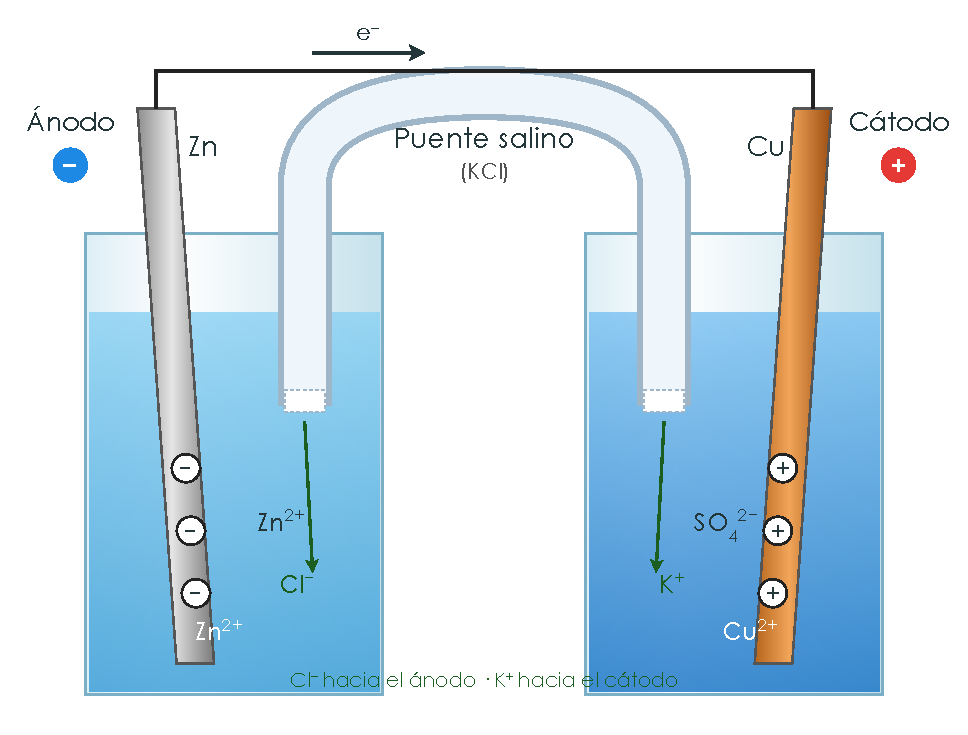
\includegraphics[width=0.6\linewidth]{FigurasSVG/UD8_Reacciones_Redox/pdf/UD8_01_puente_salino.pdf}
            \caption{Conexión del puente salino}
            \label{fig:electrodo-puente-salito}
        \end{figure}
\end{enumerate}

Este puente salino es fundamental para permitir el flujo de los iones entre las celdas para mantener un equilibrio de la carga eléctrica permitiendo así que la reacción redox continúe.

En el ejemplo anterior, podemos ver como en el caso del electrodo de \ch{Zn} se irá perdiendo cargas negativas por lo que será necesario introducir más cargas negativas en forma de \ch{Cl-} o bien eliminando del sistema cargas positivas en forma de \ch{Zn\pch[2]}.
Justamente lo contrario sucede en el caso del electrodo de cobre.
En este caso, se irá eliminando de la disolución iones positivos por lo que tendremos que introducir más iones positivos en forma de \ch{K+} o bien eliminando carga negativa en forma del anión que forme el electrodo de cobre.

\subsection{Funcionamiento de una Pila}\label{subsec:funcionamiento-de-una-pila}



Las conocidas pilas galvánicas están basadas en reacciones entre especies en disolución acuosa y están formadas por dos electrodos comunicados eléctricamente e iónicamente.
% Esta comunicación está formado por:


En el ánodo (polo negativo de la pila), se produce la oxidación, y los electrones pasan a través del sólido conductor al cátodo, donde se produce la reducción, produciéndose así el movimiento de los electrones hasta que se iguale la carga neta y se llegue al equilibrio.
La función del puente salino será evitar que se llegue a ese equilibrio hasta que no se hayan agotado los reactivos tal y como se comentó en el apartado anterior.


Consideremos la Pila de Daniell formada por los electrodos de \ch{Zn} y de \ch{Cu} sumergidos en disoluciones de sus correspondientes sulfatos.
\begin{center}
    \begin{itemize}
        \item \negsubro{Ánodo (Polo negativo)}. \(\ch{Zn - 2 \el -> Zn\pch[2]}\)
        \item \negsubro{Cátodo (Polo positivo)}. \( \ch{Cu^{2+} + 2 \el -> Cu}\)
    \end{itemize}
\end{center}

\begin{figure}[H]
    \centering
    % [FIGURA ORIGINAL] \includegraphics[scale=.45]{images/imagesUD8ReaccionesRedox/UD8_Teoria/pila_de_daniell}
    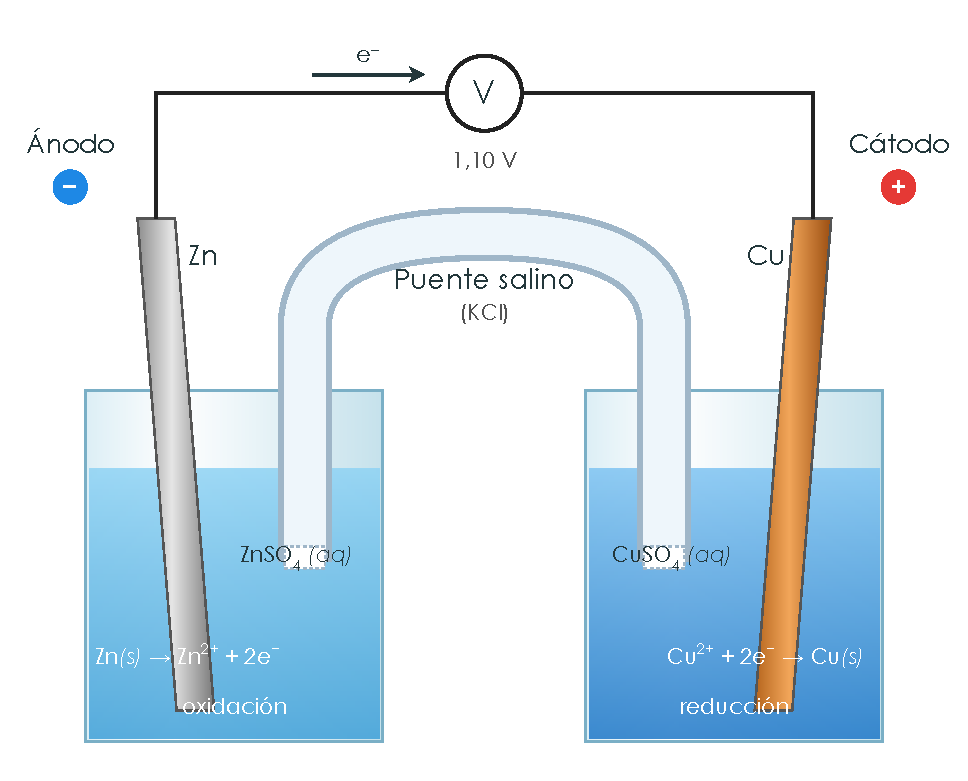
\includegraphics[width=0.65\linewidth]{FigurasSVG/UD8_Reacciones_Redox/pdf/UD8_02_pila_daniell.pdf}
    \caption{Pila de Daniell}
    \label{fig:Pila-de-Daniell}
\end{figure}

\subsection{Notación de una pila}\label{subsec:notacion-de-una-pila}

Una pila se describe a partir de la notación de los electrodos pero separando ahora ambos electrodos con una doble barra \(||\).

Por convenio, se escribe la reacción que tiene lugar en el ánodo (oxidación) a la izquierda y la reacción que tiene lugar en el cátodo (reducción) a la derecha.
Para un electrodo formado por los electrodos vistos anteriormente tendríamos que:
\begin{centeredequation}
    \underbrace{\ch{(Pt)\  Fe\pch[2]}\ |\ \ch{Fe\pch[3]} (0.05 \si{\M})}_{\text{\rojon{Ánodo}}}  \ || \ \underbrace{\ch{Cl2} (\SI{1}{\atmospher})\ | \ \ch{2 Cl-} (0.75 \si{\M})\ \ch{(Pt)}}_{\text{\azuln{Cátodo}}}
\end{centeredequation}


\subsection{Potenciales del electrodo y de la pila}\label{subsec:potenciales-del-electrodo-y-de-la-pila}

La diferencia de potencial entre los electrodos y la disolución con la que están en contacto se denomina \negrita{potencial de contacto} o \negrita{potencial eléctrico}.


\begin{center}
    \begin{definition}[Fuerza Electromotriz]
        Llamamos \negrita{fuerza electromotriz (fem)} de una pila a la diferencia de potencial entre sus electrodos.
    \end{definition}
\end{center}


Esta diferencia de potencial la podemos medir con un voltímetro y se define como el potencial de reducción del cátodo menos el potencial de reducción del ánodo:

\begin{gather*}
    \varepsilon_{\text{pila}} = \varepsilon_{\text{red cátodo}} - \varepsilon_{\text{red ánodo} } \separ
    \varepsilon_{\text{pila}}  = \varepsilon_+ - \varepsilon_-
\end{gather*}


\caja{Las especies con mayores potenciales de reducción tendrán más tendencia a reducirse actuando como oxidantes}

Mientras que:

\caja{Las especies con menores potenciales de reducción tenderán a oxidarse actuando en este caso como reductores}

Para determinar las especies que se reducen (están en el cátodo) y las especies que se oxidan (en el ánodo) debemos fijarnos en los correspondientes potenciales normales o estándar de reducción.
La especie con mayor potencial, mayor tendencia a reducirse (estará en el cátodo) mientras que la especie con menor potencial de reducción tendrá menos tendencia a reducirse (más tendencia a oxidarse)

\subsection{Electrodo de hidrógeno}\label{subsec:electrodo-de-hidrogeno}

Está constituido por una disolución de hidrones de concentración \concentracion[m]{1}, a través de la cual, se burbujea \ch{H2} a la presión de \SI{1}{\bar}.
Una varilla de platino sirve para establecer el contacto eléctrico.
La reacción que tiene lugar en el electrodo es:
\begin{centeredequation}
    \ch{2 H+ \aq{} + 2 \el -> H2 \gas{}}
\end{centeredequation}

Siendo la notación, por tanto, de dicho electrodo como:

\begin{centeredequation}
    \ch{(Pt)\ 2 H+ } \ (\SI{1}{\m})\ | \ \ch{H2 \gas}
\end{centeredequation}

\subsection{Trabajo o energía de una pila}\label{subsec:trabajo-o-energia-de-una-pila}

Al ser la pila un sistema termodinámico realizará por tanto un trabajo eléctrico que consiste en transportar la carga eléctrica desde el ánodo al cátodo siendo este trabajo la multiplicación entre la carga transportada \(Q\) y la \(fem\).

\begin{centeredequation}
    W = -Q\ \varepsilon
\end{centeredequation}

Esta carga \(Q\) la podemos tomar como \(Q = n\ F\) siendo \(n\) el \negrita{número de moles de electrones} transportados y \(F\) la constante de Faraday que establece la carga por mol de electrones, siendo su aproximado de \(F = \SI{96500}{\coulomb\per\mol}\)

La expresión anterior del trabajo la podemos escribir como:

\begin{centeredequation}
    W = -n\ F\ \varepsilon
    \label{eq:trabajo-fuerza-electromotriz}
\end{centeredequation}

En todo proceso termodinámico que se lleve a cabo a presión y temperatura constante, se cumple que \(\Delta G  = W_{\text{rev}} \).
Por lo tanto en el caso de la pila tendremos que:

\begin{centeredequation}
    \Delta G = -n\ F\ \varepsilon
    \label{eq:energia-libre-giibs-fuerza-electromotriz}
\end{centeredequation}

O en condiciones estándar

\begin{centeredequation}
    \Delta G\text{º} = -n\ F\ \varepsilon\text{º}\label{eq:G-vs-faraday}
\end{centeredequation}

Analizando la \(fem\) tendremos que:

\begin{itemize}
    \item Si \(\varepsilon_{\text{pila}} > 0\), entonces la reacción será \negrita{espontánea} debido a que \(\Delta G <0\).
    \item Si \(\varepsilon_{\text{pila}} < 0\), entonces la reacción \negrita{no} será \negrita{espontánea} debido a que \(\Delta G > 0\).
    \item Si \(\varepsilon_{\text{pila}} = 0\), la reacción estará en equilibrio debido a que \(\Delta G = 0\).
\end{itemize}



\section{Electrólisis}\label{sec:electrolisis}

\begin{center}
    \begin{definition}[Electrólisis]
        La \negrita{electrólisis} consiste en una reacción química desencadenada por el paso de corriente eléctrica a través de un electrolito o disolución conductora de la electricidad.
    \end{definition}
\end{center}


La electrólisis tiene muchas aplicaciones como la producción de metales así como la producción de no metales como el cloro y el flúor.

Para realizar una electrólisis necesitamos:

\begin{itemize}
    [label={\color{myOrange3} \(\blacksquare\)}]
    \item \negsubro{Fuente de corriente continua}.
    Proporciona la corriente eléctrica y tiene que ser continua y con un voltaje lo suficiente para que se produzca la reacción.
    Esta fuente está unida a los electrodos mediante un hilo conductor.
    Este generador ni crea ni destruye electrones, tan solo los aporta al polo negativo y los absorbe por el polo positivo.
    \item Un \negsubro{electrodo negativo} denominado \negrita{cátodo} es donde se produce la reducción.
    \item Un \negsubro{electrodo positivo} denominado \negrita{ánodo} es donde se produce la oxidación.
    \item \negsubro{Cuba o celda electrolítica}.
    Es donde se contiene la disolución o el electrolito fundido donde se sumergen los electrodos.
\end{itemize}

Un error común es asignar al ánodo el polo negativo siempre y al cátodo el polo positivo, pero como vemos ahora el proceso es a la inversa.
En realidad ánodo hace referencia al polo por el cual salen los electrones y cátodo al polo por donde entran los electrones.

Cuando establezcamos las correspondientes reacciones que suceden en una electrólisis con sus correspondientes potenciales, veremos que el potencial final de la reacción será negativo.
Este potencial nos indicará qué potencial externo debemos administrar para que se produzca la electrólisis.

\subsection{Electrólisis del agua}\label{subsec:electrolisis-del-agua}

\negsubro{NOTA IMPORTANTE:} los potenciales que se pondrán en las siguientes reacciones serán los correspondientes a dicha reacción y no deben tomarse como potenciales de reducción.
Para calcular el potencial de sistema tendremos que sumar ambos potenciales.

Si introducimos dos electrodos en una celda electrolítica y aplicamos una diferencia de potencial de \SI{2.06}{\volt} el agua se descompondrá en hidrógeno y en oxígeno tal y como se muestran en las siguientes reacciones.

\begin{centeredequation}
    \begin{array}{rrcll}
        {\color{blue} \text{Cátodo}\ (-)\ \text{Reducción}}
            : & \ch{2 H2O + 2 \el{}} & \ch{->} & \ch{ H2 + 2 OH-}    & \varepsilon\text{º} = \SI{-0.83}{\volt}                \separ
            {\color{blue}\text{Ánodo}\ (+)\ \text{Oxidación}}:   & \ch{2 H2O}        & \ch{->} & \ch{O2 + 4 H+ + 4 \el}   & \varepsilon\text{º} = \SI{-1.23}{\volt} \separ
            \midrule
            {\color{blue} \text{Reacción global} }:              & \ch{2 H2O\lqd{}}    & \ch{->} & \ch{2 H2\gas{} + O2\gas{}}  & \varepsilon\text{º}_\text{reacción} = \SI{-2.06}{\volt}
    \end{array}
\end{centeredequation}

En este caso, tendríamos que aplicar un potencial de al menos \SI{2.06}{\volt} para llevar a cabo la electrólisis.


\subsubsection{Técnicas de electrólisis del agua}

Estas técnicas varían en función de la cantidad de \ch{H2} y de \ch{O2} que se quiera generar.

\negsubro{Electrólisis con agua ácida}

Si la reacción de electrólisis se realiza en medio ácido, las reacciones que tendríamos serían:

\begin{centeredequation}
    \begin{array}{rrcll}
        {\color{blue} \text{Cátodo}\ (-)\ \text{Reducción}}
            : & \ch{2 H+ + 2 \el{}} & \ch{->} & \ch{  H2 }    & \varepsilon\text{º} = \SI{0.00}{\volt}                \separ
            {\color{blue}\text{Ánodo}\ (+)\ \text{Oxidación}}:   & \ch{2 H2O }        & \ch{->} & \ch{ O2 + 4 H+ + 4 \el{}}   & \varepsilon\text{º} = \SI{-1.23}{\volt} \separ
            \midrule
            {\color{blue} \text{Reacción global} }:              & \ch{2 H2O\lqd{}}    & \ch{->} & \ch{2 H2\gas{} + O2\gas{}}  & \varepsilon\text{º}_\text{reacción} = \SI{-1.23}{\volt}
    \end{array}
\end{centeredequation}

En este caso, tendríamos que aplicar un potencial de al menos \SI{1.23}{\volt} para llevar a cabo la electrólisis.

\negsubro{Electrólisis con agua alcalina}

La electrólisis también se puede llevar a cabo con soluciones básicas como \ch{KOH} o \ch{NaOH}.
En este caso, las reacciones que tendrían lugar serían:

\begin{centeredequation}
    \begin{array}{rrcll}
        {\color{blue} \text{Cátodo}\ (-)\ \text{Reducción}}
            : & \ch{2 H2O + 2 \el{}} & \ch{->} & \ch{ H2 + 2 OH-}    & \varepsilon\text{º} = \SI{-0.83}{\volt}                \separ
            {\color{blue}\text{Ánodo}\ (+)\ \text{Oxidación}}:   & \ch{4 OH- }        & \ch{->} & \ch{O2 + 2 H2O + 4 \el{}}   & \varepsilon\text{º} = \SI{-0.41}{\volt} \separ
            \midrule
            {\color{blue} \text{Reacción global} }:              & \ch{2 H2O\lqd{}}    & \ch{->} & \ch{2 H2\gas{} + O2\gas{}}  & \varepsilon\text{º}_\text{reacción} = \SI{-1.24}{\volt}
    \end{array}
\end{centeredequation}

\subsection{Electrólisis de una sal fundida}\label{subsec:electrolisis-de-una-sal-fundida}

Si tenemos una sal como el \ch{NaCl} fundida, al sumergir los electrodos y conectar la corriente continua, los iones \ch{Cl-} se oxidan en el ánodo, descargándose según la reacción siguiente:

\begin{centeredequation}
    \begin{array}{rrcll}
        {\color{blue} \text{Cátodo}\ (-)\ \text{Reducción}}
            : & \ch{ Na+ + 1 \el{}} & \ch{->} & \ch{Na}  & \varepsilon\text{º} = \SI{-2.71}{\volt}                 \separ
            {\color{blue}\text{Ánodo}\ (+)\ \text{Oxidación}}:   & \ch{2 Cl-}        & \ch{->} & \ch{Cl2 + 2 \el{}}  & \varepsilon\text{º} = \SI{-1.36}{\volt}  \separ
            \midrule
            {\color{blue} \text{Reacción global} }:              & \ch{2 NaCl}    & \ch{->} & \ch{2 Na + Cl2} & \varepsilon\text{º}\subin{reacción} = \SI{-4.07}{\volt}
    \end{array}
\end{centeredequation}

Otro ejemplo sería el de la sal \ch{CuCl2}: analizando los potenciales normales de reducción de ambas especies, en el ánodo se desprenderá \ch{Cl2} y en el cátodo se recubrirá de una película brillante de \ch{Cu}.
Las reacciones que tienen lugar son:

\begin{centeredequation}
    \begin{array}{rrcll}
        {\color{blue} \text{Cátodo}\ (-)\ \text{Reducción}}
            : & \ch{Cu\pch[2] + 2 \el} & \ch{->} & \ch{Cu}                   & \varepsilon\text{º} = \SI{0.346}{\volt} \separ
            {\color{blue}\text{Ánodo}\ (+)\ \text{Oxidación}}:   & \ch{2 Cl-}             & \ch{->} & \ch{Cl2 + 2 \el}          & \varepsilon\text{º} = \SI{-1.359}{\volt} \separ
            \midrule
            {\color{blue} \text{Reacción global} }:              & \ch{CuCl2\aq{}}        & \ch{->} & \ch{Cu\sld{} + Cl2\gas{}} & \varepsilon\text{º}_{\text{reacción}} = \SI{-1.013}{\volt}
    \end{array}
\end{centeredequation}

\subsection{Electrólisis de una sal disuelta}\label{subsec:electrolisis-de-una-sal-disuelta}

Si realizamos la electrólisis con sales disueltas en disolución acuosa, el agua presente en la disolución compite con los iones provenientes de la sal y la electrólisis sufre algunas modificaciones.

Como ejemplo, estudiaremos la electrólisis de una disolución acuosa de \ch{NaCl}.

En este caso tendremos dos posibles reacciones de oxidación y debemos determinar cuál de ellas es la que se produce:

\begin{centeredequation}
    \begin{array}{rcll}
        \ch{2 H2O } & \ch{->} & \ch{O2 + 4 H+ + 4 \el{}}  & \varepsilon\text{º} = \SI{-1.23}{\volt}   \separ
        \ch{2 Cl-}        & \ch{->} & \ch{Cl2 + 2 \el{}}  & \varepsilon\text{º} = \SI{-1.36}{\volt}
    \end{array}
\end{centeredequation}


Debido a que en un disolución de una sal además de la correspondiente sal tenemos \water{} esta puede competir en la reacción de hidrólisis y por tanto hay que analizar los correspondientes potenciales normales de reducción.
Así por ejemplo en el caso de la hidrólisis de una disolución acuosa de \ch{NaCl}, las reacciones que tienen lugar son:

\begin{centeredequation}
    \begin{array}{rrcll}
        {\color{blue} \text{Cátodo}\ (-)\ \text{Reducción}}
            : & \ch{2 H+ + 2 \el{}}& \ch{->} & \ch{ H2} & \varepsilon\text{º} = \SI{0}{\volt} \separ
            {\color{blue}\text{Ánodo}\ (+)\ \text{Oxidación}}: & \ch{2 Cl-}& \ch{->} & \ch{Cl2 + 2 \el} & \varepsilon\text{º} = \SI{-1.359}{\volt} \separ
            \midrule
            {\color{blue} \text{Reacción global} }: & \ch{2 H+ \aq{} + 2 Cl- \aq{}} & \ch{->} & \ch{H2\gas{} + Cl2\gas{}} & \varepsilon\text{º}_{\text{reacción}} = \SI{-1.359}{\volt}
    \end{array}
\end{centeredequation}

Como vemos, ahora en el cátodo, se produce la reducción de los iones  \ch{H+} en lugar de producirse la reducción del \ch{Na+} a \ch{Na} según la reacción:

\begin{centeredequation}
    \ch{Na+ \aq{} + \el -> Na\sld{}}
\end{centeredequation}

Esto es debido a que el potencial normal de reducción del sodio (\(\varepsilon\text{º} = \SI{-2.71}{\volt}\)) es menor que el del hidrógeno  (\(\varepsilon\text{º} = \SI{0}{\volt}\)). Esto demuestra que los iones \ch{H+} tienen una mayor apetencia por los electrones que los iones \ch{Na+} y, por tanto, se reducen los iones  \ch{H+} y no los iones \ch{Na+}.

De manera general podemos decir que:

\begin{itemize}
    \item En el cátodo que es donde se producirá la reducción.
    Los cationes de mayor potencial normal de reducción serán los primeros en descargarse.
    \item En el ánodo que es donde se producirá la oxidación, los iones negativos de menor potencial normal de reducción serán los primeros en descargarse.
\end{itemize}


\section{Leyes de Faraday}\label{sec:leyes-de-faraday}

\negrita{Michael Faraday} formuló las leyes fundamentales de la electrólisis.

\caja{La cantidad de sustancia que sufre oxidación o reducción en cada electrodo durante una electrólisis es directamente proporcional a la cantidad de electricidad que pasa a través de la disolución.}

\begin{enumerate}[label=\numberballmDarkTeal]
        \item \negsubro{Primera ley de Faraday}.
        Las \negrita{masas} de las sustancias depositadas o liberadas en cada electrodo durante una electrólisis son proporcionales a la \negrita{cantidad de electricidad} que ha pasado a través de la celda electrolítica.
        \item \negsubro{Segunda ley de Faraday}.
        Para una misma cantidad de carga eléctrica, la masa de las sustancias depositadas o liberadas en los electrodos es proporcional a su masa atómica y al número de electrones intercambiados por cada una de ellas según la expresión:

        \begin{gather}
            Q = z\ \dfrac{m}{M_a}\cdot F  \notag \separ
            m(g) = \dfrac{M_a}{z\cdot F}\cdot Q
        \end{gather}

        \begin{itemize}
            \item \(Q\) = carga que circula en culombios.
            \item \(z\) = número de electrones intercambiados.
            \item \(m\) = masa depositada o liberada en gramos.
            \item \(M_a\) = masa atómica.
            \item \(F\) = constante de Faraday
        \end{itemize}

        Hay que tener en cuenta que:

        \begin{itemize}
            \item \textbf{Carga eléctrica(\(\bm{Q}\))}: es la carga que circula por la cuba electrolítica, y se puede expresar en función de la intensidad de corriente eléctrica, según la expresión.
            \begin{centeredequation}
                Q = I\cdot t
            \end{centeredequation}
            \item \textbf{Número de electrones (\(\bm{z}\))}: es la cantidad de electrones (mol) que necesita una sustancia para oxidarse o reducirse en un electrodo.

            Para semirreacción: \ch{Ag+ \aq{} + 1 \el{} -> Ag \sld{}} \(\Rightarrow z = 1\).

            Para la semirreacción: \ch{Cl- \aq{}  -> Cl2 \gas{} + 2 \el{}} \(\Rightarrow z = 2\).
        \end{itemize}

\end{enumerate}




    \newpage

    %! Author = Profesor
%! Date = 06/06/2024


\section{Ejercicios y Ejercicios EVAU}

\subsection{Ejercicios}


\begin{exercise}
    En medio ácido, el permanganato de potasio oxida el ion cloruro a cloro reduciéndose a manganeso (III). Escribe y ajusta la reacción usando el método del ion-electrón.
    \begin{solu}

        \textbf{Semirreacción de reducción} (\ch{Mn^{+7} -> Mn^{+3}}, gana 4 electrones):

        \begin{equation*}
            \ch{MnO4- + 8 H+ + 4 e- -> Mn^{3+} + 4 H2O}
        \end{equation*}

        \textbf{Semirreacción de oxidación} (\ch{Cl^{-1} -> Cl^{0}}, pierde 1 electrón por átomo):

        \begin{equation*}
            \ch{2 Cl- -> Cl2 + 2 e-}
        \end{equation*}

        Para igualar los electrones intercambiados (mínimo común múltiplo de 4 y 2 es 4), multiplicamos la semirreacción de oxidación por 2:

        \begin{equation*}
            \ch{4 Cl- -> 2 Cl2 + 4 e-}
        \end{equation*}

        Sumando ambas semirreacciones:

        \begin{equation*}
            \ch{MnO4- + 8 H+ + 4 Cl- -> Mn^{3+} + 4 H2O + 2 Cl2}
        \end{equation*}

        Pasando a la forma molecular con \ch{KMnO4} y \ch{HCl} (que aporta tanto los \ch{H+} como los \ch{Cl-} necesarios, incluyendo los 3 \ch{Cl-} que acompañan al \ch{Mn^{3+}} en el \ch{MnCl3} y 1 \ch{Cl-} para el \ch{KCl}):

        \begin{equation*}
            \ch{KMnO4 + 8 HCl -> MnCl3 + KCl + 2 Cl2 + 4 H2O}
        \end{equation*}

        Comprobación: K (1=1), Mn (1=1), O (4=4), H (8=8), Cl (\(8 = 3+1+4\)).

    \end{solu}
\end{exercise}

\begin{exercise}
    Las siguientes reacciones se dan en medio ácido:

    \begin{enumerate}
        \item \ch{MnO2\sld{} + Cl- \aq{} -> Mn\pch[2]\aq{} + Cl2\gas{}}
        \item \ch{I- \aq{} + Br2\lqd{} -> IO3- \aq{} + Br- \aq{}}
    \end{enumerate}
    \begin{solu}

        \textbf{1) \ch{MnO2 + Cl- -> Mn^2+ + Cl2}}

        Reducción (\ch{Mn^{+4} -> Mn^{+2}}, gana 2 e\textsuperscript{-}):

        \begin{equation*}
            \ch{MnO2 + 4 H+ + 2 e- -> Mn^{2+} + 2 H2O}
        \end{equation*}

        Oxidación (\ch{Cl^{-1} -> Cl^{0}}, pierde 2 e\textsuperscript{-} por cada \ch{Cl2}):

        \begin{equation*}
            \ch{2 Cl- -> Cl2 + 2 e-}
        \end{equation*}

        Como ambas ceden/ganan 2 electrones, se suman directamente:

        \begin{equation*}
            \ch{MnO2 + 4 H+ + 2 Cl- -> Mn^{2+} + 2 H2O + Cl2}
        \end{equation*}

        En forma molecular (con \ch{HCl}):

        \begin{equation*}
            \ch{MnO2 + 4 HCl -> MnCl2 + Cl2 + 2 H2O}
        \end{equation*}

        \textbf{2) \ch{I- + Br2 -> IO3- + Br-}}

        Oxidación (\ch{I^{-1} -> I^{+5}}, pierde 6 e\textsuperscript{-}):

        \begin{equation*}
            \ch{I- + 3 H2O -> IO3- + 6 H+ + 6 e-}
        \end{equation*}

        Reducción (\ch{Br^{0} -> Br^{-1}}, gana 2 e\textsuperscript{-} por cada \ch{Br2}):

        \begin{equation*}
            \ch{Br2 + 2 e- -> 2 Br-}
        \end{equation*}

        Igualando electrones (m.c.m. de 6 y 2 es 6), multiplicamos la reducción por 3:

        \begin{equation*}
            \ch{3 Br2 + 6 e- -> 6 Br-}
        \end{equation*}

        Sumando:

        \begin{equation*}
            \ch{I- + 3 H2O + 3 Br2 -> IO3- + 6 H+ + 6 Br-}
        \end{equation*}

        En forma molecular (con \ch{HI} y \ch{HBr}):

        \begin{equation*}
            \ch{HI + 3 H2O + 3 Br2 -> HIO3 + 6 HBr}
        \end{equation*}

    \end{solu}
\end{exercise}

\begin{exercise}
    Ajusta las siguientes reacciones por el método del ion-electrón:

    \begin{enumerate}[label=\letraminuscula]
        \item \ch{Cl2 + NaOH -> NaCl + NaClO + H2O}
        \item \ch{HNO3 + Cu -> Cu(NO3)2 + NO2 + H2O}
        \item \ch{HCl + K2Cr2O7 -> KCl + CrCl3 + Cl2 + H2O}
        \item \ch{KNO3 + Al + KOH + H2O -> NH3 + KAlO2}
        \item \ch{Na2SO4 + C -> Na2S + CO2}
        \item \ch{MnO4- + SO2 -> Mn\pch[2] + HSO4-}
        \item \ch{MnO2- + I- -> MnO4- + IO3-}
        \item \ch{I2 + HNO3 -> HIO3 + NO2 + H2O}
        \item \ch{MnO4- + SO3\mch[2] -> Mn\pch[2] + SO4\mch[2]} (medio ácido)
        \item \ch{TiO2 + Al -> Al2O3 + Ti}
        \item \ch{HNO3\aq{} + C\sld{} -> CO2\gas{} + NO2\gas{} + H2O\lqd{}}
        \item \ch{Bi(OH)3\aq{} + Na2SnO2\aq{} -> Bi\sld{} + Na2SnO3\aq{} + H2O\lqd{}}
    \end{enumerate}
    \begin{solu}

        \textbf{a) \ch{Cl2 + NaOH -> NaCl + NaClO + H2O}} (dismutación del cloro en medio básico)

        Reducción: \(\ch{Cl2 + 2 e- -> 2 Cl-}\). Oxidación: \(\ch{Cl2 + 4 OH- -> 2 ClO- + 2 H2O + 2 e-}\).

        Sumando (mismos electrones): \(\ch{2 Cl2 + 4 OH- -> 2 Cl- + 2 ClO- + 2 H2O}\), que simplificado da:

        \begin{equation*}
            \ch{Cl2 + 2 NaOH -> NaCl + NaClO + H2O}
        \end{equation*}

        \textbf{b) \ch{HNO3 + Cu -> Cu(NO3)2 + NO2 + H2O}} (ácido nítrico concentrado)

        Reducción: \(\ch{NO3- + 2 H+ + e- -> NO2 + H2O}\) (\(\times 2\)). Oxidación: \(\ch{Cu -> Cu^{2+} + 2 e-}\).

        \begin{equation*}
            \ch{Cu + 4 HNO3 -> Cu(NO3)2 + 2 NO2 + 2 H2O}
        \end{equation*}

        \textbf{c) \ch{HCl + K2Cr2O7 -> KCl + CrCl3 + Cl2 + H2O}}

        Reducción: \(\ch{Cr2O7^2- + 14 H+ + 6 e- -> 2 Cr^{3+} + 7 H2O}\). Oxidación: \(\ch{2 Cl- -> Cl2 + 2 e-}\) (\(\times 3\)).

        \begin{equation*}
            \ch{K2Cr2O7 + 14 HCl -> 2 KCl + 2 CrCl3 + 3 Cl2 + 7 H2O}
        \end{equation*}

        \textbf{d) \ch{KNO3 + Al + KOH + H2O -> NH3 + KAlO2}} (medio básico)

        Reducción: \(\ch{NO3- + 6 H2O + 8 e- -> NH3 + 9 OH-}\) (\(\times 3\)). Oxidación: \(\ch{Al + 4 OH- -> AlO2- + 2 H2O + 3 e-}\) (\(\times 8\)).

        Sumando y simplificando \ch{H2O} y \ch{OH-} sobrantes:

        \begin{equation*}
            \ch{3 KNO3 + 8 Al + 5 KOH + 2 H2O -> 3 NH3 + 8 KAlO2}
        \end{equation*}

        \textbf{e) \ch{Na2SO4 + C -> Na2S + CO2}}

        \ch{S}: \(+6 \to -2\) (gana 8 e\textsuperscript{-}); \ch{C}: \(0 \to +4\) (pierde 4 e\textsuperscript{-}). Se necesitan 2 mol de C por cada mol de S:

        \begin{equation*}
            \ch{Na2SO4 + 2 C -> Na2S + 2 CO2}
        \end{equation*}

        \textbf{f) \ch{MnO4- + SO2 -> Mn^2+ + HSO4-}} (medio ácido)

        Reducción: \(\ch{MnO4- + 8 H+ + 5 e- -> Mn^{2+} + 4 H2O}\) (\(\times 2\)). Oxidación: \(\ch{SO2 + 2 H2O -> HSO4- + 3 H+ + 2 e-}\) (\(\times 5\)).

        \begin{equation*}
            \ch{2 MnO4- + 5 SO2 + 2 H2O + H+ -> 2 Mn^{2+} + 5 HSO4-}
        \end{equation*}

        \textbf{g) \ch{MnO2- + I- -> MnO4- + IO3-}}

        \textit{Nota:} tal como está escrita, esta ecuación no se puede ajustar como proceso redox, ya que tanto el manganeso (que pasaría de un estado de oxidación \(+3\) en \ch{MnO2-} a \(+7\) en \ch{MnO4-}) como el yodo (que pasaría de \(-1\) en \ch{I-} a \(+5\) en \ch{IO3-}) se \textbf{oxidarían}, sin que exista ninguna especie que se reduzca. Es muy probable que se trate de una errata en el enunciado (por ejemplo, el reactivo de manganeso debería ser una especie donde el Mn se reduzca, o falte algún otro reactivo oxidante). Por ello, esta reacción no puede ajustarse tal como está planteada.

        \textbf{h) \ch{I2 + HNO3 -> HIO3 + NO2 + H2O}}

        Oxidación: \(\ch{I2 + 6 H2O -> 2 IO3- + 12 H+ + 10 e-}\). Reducción: \(\ch{NO3- + 2 H+ + e- -> NO2 + H2O}\) (\(\times 10\)).

        \begin{equation*}
            \ch{I2 + 10 HNO3 -> 2 HIO3 + 10 NO2 + 4 H2O}
        \end{equation*}

        \textbf{i) \ch{MnO4- + SO3^2- -> Mn^2+ + SO4^2-}} (medio ácido)

        Reducción: \(\ch{MnO4- + 8 H+ + 5 e- -> Mn^{2+} + 4 H2O}\) (\(\times 2\)). Oxidación: \(\ch{SO3^2- + H2O -> SO4^2- + 2 H+ + 2 e-}\) (\(\times 5\)).

        \begin{equation*}
            \ch{2 MnO4- + 5 SO3^2- + 6 H+ -> 2 Mn^{2+} + 5 SO4^2- + 3 H2O}
        \end{equation*}

        \textbf{j) \ch{TiO2 + Al -> Al2O3 + Ti}}

        \ch{Ti}: \(+4 \to 0\) (gana 4 e\textsuperscript{-}); \ch{Al}: \(0 \to +3\) (pierde 3 e\textsuperscript{-}). m.c.m.(4,3) = 12:

        \begin{equation*}
            \ch{3 TiO2 + 4 Al -> 2 Al2O3 + 3 Ti}
        \end{equation*}

        \textbf{k) \ch{HNO3 + C -> CO2 + NO2 + H2O}}

        Oxidación: \(\ch{C + 2 H2O -> CO2 + 4 H+ + 4 e-}\). Reducción: \(\ch{NO3- + 2 H+ + e- -> NO2 + H2O}\) (\(\times 4\)).

        \begin{equation*}
            \ch{C + 4 HNO3 -> CO2 + 4 NO2 + 2 H2O}
        \end{equation*}

        \textbf{l) \ch{Bi(OH)3 + Na2SnO2 -> Bi + Na2SnO3 + H2O}} (medio básico)

        Reducción: \(\ch{Bi(OH)3 + 3 e- -> Bi + 3 OH-}\) (\(\times 2\)). Oxidación: \(\ch{SnO2^2- + 2 OH- -> SnO3^2- + H2O + 2 e-}\) (\(\times 3\)).

        Sumando y cancelando los \ch{OH-} que se repiten en ambos lados:

        \begin{equation*}
            \ch{2 Bi(OH)3 + 3 Na2SnO2 -> 2 Bi + 3 Na2SnO3 + 3 H2O}
        \end{equation*}

    \end{solu}
\end{exercise}

%* Libro Santillana página 300
\begin{exercise}
    Se hace pasar una corriente eléctrica de \SI{5}{\ampere} durante \num{2.5} horas a través de una celda electrolítica que contiene una disolución de cloruro de cobre (II). Calcule:
    \begin{enumerate}[label=\letraminuscula]
        \item La masa de cobre metálico depositado en el cátodo.
        \item El volumen de cloro molecular medido en condiciones normales que se genera en el ánodo.
    \end{enumerate}
    \datos{} \(F = \num{96500}\ \dfrac{\text{C}}{\text{mol}}\); masa atómica Cu = \num{63.5}
    \begin{solu}

        La carga total que atraviesa la celda es:

        \begin{equation*}
            Q = I \cdot t = 5 \ \si{\ampere} \times (2,5 \times 3600) \ \si{\s} = \SI{45000}{\coulomb}
        \end{equation*}

        Los moles de electrones intercambiados son:

        \begin{equation*}
            n(e^-) = \dfrac{Q}{F} = \dfrac{45000}{96500} = 0,4663 \ \text{mol}
        \end{equation*}

        \textbf{a) Masa de cobre depositada en el cátodo}

        En el cátodo tiene lugar la reducción \(\ch{Cu^{2+} + 2 e- -> Cu}\), por lo que:

        \begin{equation*}
            n(\ch{Cu}) = \dfrac{n(e^-)}{2} = \dfrac{0,4663}{2} = 0,2332 \ \text{mol}
        \end{equation*}

        \begin{equation*}
            m(\ch{Cu}) = 0,2332 \times 63,5 = \SI{14.8}{\gram}
        \end{equation*}

        \textbf{b) Volumen de \ch{Cl2} en condiciones normales}

        En el ánodo tiene lugar la oxidación \(\ch{2 Cl- -> Cl2 + 2 e-}\), por lo que:

        \begin{equation*}
            n(\ch{Cl2}) = \dfrac{n(e^-)}{2} = 0,2332 \ \text{mol}
        \end{equation*}

        \begin{equation*}
            V(\ch{Cl2}) = 0,2332 \times 22,4 = \SI{5.22}{\litre}
        \end{equation*}

    \end{solu}
\end{exercise}
\begin{exercise}
    Dos cubas electrolíticas que contienen disoluciones acuosas de nitrato de plata y nitrato de cobre (II), respectivamente están montadas en serie (pasa la misma intensidad por ambas). Si en 1 hora se depositan en la segunda cuba \masa[g]{54.5} de cobre, calcule:
    \begin{enumerate}[label=\letraminuscula]
        \item La intensidad de corriente que atraviesa las cubas.
        \item Los gramos de plata que se depositarán en la primera cuba tras dos horas de paso de la misma intensidad de corriente.
    \end{enumerate}
    \datos{} \(F = \num{96500}\ \dfrac{\text{C}}{\text{mol}}\); masa atómica Cu = \num{63.5}; masa atómica Ag = \num{107.9}
    \begin{solu}

        \textbf{a) Intensidad de corriente}

        En la segunda cuba (\ch{Cu(NO3)2}), la reducción es \(\ch{Cu^{2+} + 2 e- -> Cu}\). Los moles de \ch{Cu} depositados son:

        \begin{equation*}
            n(\ch{Cu}) = \dfrac{54,5}{63,5} = 0,8583 \ \text{mol} \ \Rightarrow \ n(e^-) = 2 \times 0,8583 = 1,7165 \ \text{mol}
        \end{equation*}

        \begin{equation*}
            Q = n(e^-) \cdot F = 1,7165 \times 96500 = \SI{165642}{\coulomb}
        \end{equation*}

        Como \(t = \SI{1}{\hour} = \SI{3600}{\s}\):

        \begin{equation*}
            I = \dfrac{Q}{t} = \dfrac{165642}{3600} = \SI{46.0}{\ampere}
        \end{equation*}

        \textbf{b) Gramos de plata depositados en la primera cuba tras 2 horas}

        Al estar las cubas en serie, la misma intensidad \(I = \SI{46.0}{\ampere}\) atraviesa ambas. Con \(t = \SI{2}{\hour} = \SI{7200}{\s}\):

        \begin{equation*}
            Q' = I \cdot t = 46,0 \times 7200 = \SI{331200}{\coulomb} \ \Rightarrow \ n(e^-) = \dfrac{331200}{96500} = 3,432 \ \text{mol}
        \end{equation*}

        Como en la primera cuba la reducción es \(\ch{Ag+ + e- -> Ag}\) (1 electrón por ion), los moles de \ch{Ag} depositados coinciden con los moles de electrones:

        \begin{equation*}
            n(\ch{Ag}) = 3,432 \ \text{mol} \ \Rightarrow \ m(\ch{Ag}) = 3,432 \times 107,9 = \SI{370.3}{\gram}
        \end{equation*}

    \end{solu}
    %* Libro Santillana página 307
\end{exercise}
\begin{exercise}
    Cuando se realiza la electrolisis en una disolución de una sal soluble de un metal divalente, pasando una corriente de \SI{3}{\ampere} durante cinco horas, se depositan \masa[g]{18.29}.
    \begin{enumerate}[label=\letraminuscula]
        \item Calcule la masa atómica del metal.
        \item Indique el nombre del electrodo donde se deposita el metal, escriba la reacción que tiene lugar en él y razone si se trata de una oxidación o de una reducción.
        \item Considerando el significado de la constante de Faraday, calcule expresando el resultado en culombios, la carga del ión divalente del metal.
    \end{enumerate}
    \datos{} \(F = \num{96500}\ \dfrac{\text{C}}{\text{mol}}\); \(N_A = \num{6.022e23}\).
    \begin{solu}

        \textbf{a) Masa atómica del metal}

        La carga total es:

        \begin{equation*}
            Q = I \cdot t = 3 \times (5 \times 3600) = \SI{54000}{\coulomb} \ \Rightarrow \ n(e^-) = \dfrac{54000}{96500} = 0,5596 \ \text{mol}
        \end{equation*}

        Como el metal es divalente, \(\ch{M^{2+} + 2 e- -> M}\):

        \begin{equation*}
            n(M) = \dfrac{n(e^-)}{2} = \dfrac{0,5596}{2} = 0,2798 \ \text{mol}
        \end{equation*}

        \begin{equation*}
            M_{at} = \dfrac{m}{n} = \dfrac{18,29}{0,2798} = \SI{65.4}{\gram\per\mole}
        \end{equation*}

        (Este valor corresponde, muy probablemente, al del cinc, \(M(\ch{Zn}) \approx \SI{65.4}{\gram\per\mole}\).)

        \textbf{b) Electrodo de deposición}

        El metal se deposita en el \textbf{cátodo}, donde tiene lugar la semirreacción:

        \begin{equation*}
            \ch{M^{2+} + 2 e- -> M}
        \end{equation*}

        Se trata de una \textbf{reducción}, ya que el catión metálico gana electrones para formar el metal neutro.

        \textbf{c) Carga del ion divalente}

        La constante de Faraday es la carga de 1 mol de electrones, \(F = N_A \cdot e\), por lo que la carga de un electrón es:

        \begin{equation*}
            e = \dfrac{F}{N_A} = \dfrac{96500}{6,022\times10^{23}} = \num{1.602e-19} \ \si{\coulomb}
        \end{equation*}

        Como el ion es divalente (carga \(2+\)), su carga es el doble de la del electrón (en valor absoluto):

        \begin{equation*}
            q(\ch{M^{2+}}) = 2 \times 1,602\times10^{-19} = \num{3.204e-19} \ \si{\coulomb}
        \end{equation*}

    \end{solu}
\end{exercise}

\subsection{Ejercicios PAU}
\begin{exerciseEVAU}
    Indique si las siguientes afirmaciones son verdaderas o falsas, justificando su
respuesta:
\begin{enumerate}[label=\letraminuscula]
    \item Cuanto mayor sea el \( E^0 \) de una sustancia, mayor será su carácter oxidante.
    \item La reacción de una pila en condiciones estándar transcurre sin necesidad de una fuente
de energía externa (proceso espontaneo), generando corriente eléctrica, si \( \Delta G > 0 \).
\end{enumerate}
\begin{solu}
    Indique si las siguientes afirmaciones son verdaderas o falsas, justificando su
respuesta:
letra
\end{solu}
\end{exerciseEVAU}
\begin{exerciseEVAU}
Sea la siguiente reacción redox:
\begin{equation*}
    \ch{Cu \sld{} + HNO3 -> Cu(NO3)2 + NO + H2O}
\end{equation*}
\begin{enumerate}[label=\letraminuscula]
    \item Escriba las semirreacciones de oxidación y reducción. Señale claramente cuál es el oxidante
y el reductor.
    \item  Ajuste las ecuaciones iónica y molecular por el método del ion-electrón.
    \item Calcule los gramos de Cu(s) necesarios para obtener 10 g de NO si el rendimiento de la
reacción es del 75\%.
\end{enumerate}
\begin{solu}

\end{solu}
\end{exerciseEVAU}

\begin{exerciseEVAU}
    Una forma de estimar la contaminación del agua es medir la Demanda Química de Oxígeno (DQO). Para
ello, el carbono (C) se transforma en dióxido de carbono (\ch{CO2}) al reaccionar en medio ácido con dicromato
de potasio (\ch{K2Cr2O7}), según la siguiente reacción:
    \begin{centeredequation}
        \ch{C + K2Cr2O7 + HCl -> CO2 + CrCl3 + KCl + H2O}
    \end{centeredequation}
    \begin{enumerate}[label=\letraminuscula]
        \item Escriba y ajuste las semirreacciones iónicas de oxidación y de reducción.
        \item Indique qué especie actúa como oxidante y cuál como reductor.
        \item Ajuste la reacción iónica global y la reacción molecular.
        \item Si \( E^0(\ch{Cr2O7^{2–}}/Cr^{3+}) \) = \qty{1.44}{\volt}  ¿qué valor debería tener \( E^00(\ch{CO2}/C) \) para que la reacción estuviera en equilibrio?
    \end{enumerate}
\begin{solu}

    \textbf{a) Semirreacciones}

    Oxidación (\ch{C^{0} -> C^{+4}}, pierde 4 e\textsuperscript{-}):

    \begin{equation*}
        \ch{C + 2 H2O -> CO2 + 4 H+ + 4 e-}
    \end{equation*}

    Reducción (\ch{Cr^{+6} -> Cr^{+3}}, gana \(3\times2=6\) e\textsuperscript{-} por \ch{Cr2O7^2-}):

    \begin{equation*}
        \ch{Cr2O7^2- + 14 H+ + 6 e- -> 2 Cr^{3+} + 7 H2O}
    \end{equation*}

    \textbf{b) Oxidante y reductor}

    El \textbf{oxidante} es el \ch{K2Cr2O7} (el \ch{Cr2O7^2-} se reduce), y el \textbf{reductor} es el \ch{C} (se oxida).

    \textbf{c) Reacción iónica y molecular}

    Igualando electrones (m.c.m. de 4 y 6 es 12): oxidación \(\times 3\), reducción \(\times 2\):

    \begin{equation*}
        \ch{3 C + 6 H2O -> 3 CO2 + 12 H+ + 12 e-}
    \end{equation*}
    \begin{equation*}
        \ch{2 Cr2O7^2- + 28 H+ + 12 e- -> 4 Cr^{3+} + 14 H2O}
    \end{equation*}

    Sumando y simplificando:

    \begin{equation*}
        \ch{3 C + 2 Cr2O7^2- + 16 H+ -> 3 CO2 + 4 Cr^{3+} + 8 H2O}
    \end{equation*}

    En forma molecular:

    \begin{equation*}
        \ch{3 C + 2 K2Cr2O7 + 16 HCl -> 3 CO2 + 4 CrCl3 + 4 KCl + 8 H2O}
    \end{equation*}

    \textbf{d) Potencial para el equilibrio}

    Una reacción redox está en equilibrio (\(\Delta E^0_{cell} = 0\), es decir, no transcurre en ningún sentido de forma espontánea) cuando los potenciales estándar de ambos pares son iguales:

    \begin{equation*}
        E^0(\ch{Cr2O7^{2-}}/\ch{Cr^{3+}}) = E^0(\ch{CO2}/\ch{C}) = \SI{1.44}{\volt}
    \end{equation*}

\end{solu}
\end{exerciseEVAU}

\begin{exerciseEVAU}
El dicromato de potasio \ch{K2Cr2O7} reacciona con cloruro de hierro (II), \ch{FeCl2}, en disolución de ácido
clorhídrico, \ch{HCl}, según la siguiente reacción:
\begin{centeredequation}
    \ch{K2Cr2O7 + FeCl2 + HCl -> CrCl3 + FeCl3 + KCl + H2O}
\end{centeredequation}
\begin{enumerate}[label=\letraminuscula]
    \item  Ajuste por el método del ion electrón las semirreacciones de oxidación y reducción. Indique
las especies oxidante y reductora. Ajuste la reacción iónica y la molecular.
    \item  Determine qué masa de \ch{K2Cr2O7} se necesitará para que reaccione completamente con 50 mL de disolución de \ch{FeCl2} 0,60 M
\end{enumerate}
\begin{solu}

    \textbf{a) Semirreacciones, oxidante/reductor y ecuaciones ajustadas}

    Reducción (\ch{Cr^{+6} -> Cr^{+3}}, gana 6 e\textsuperscript{-}):

    \begin{equation*}
        \ch{Cr2O7^2- + 14 H+ + 6 e- -> 2 Cr^{3+} + 7 H2O}
    \end{equation*}

    Oxidación (\ch{Fe^{+2} -> Fe^{+3}}, pierde 1 e\textsuperscript{-}), multiplicada por 6:

    \begin{equation*}
        \ch{6 Fe^{2+} -> 6 Fe^{3+} + 6 e-}
    \end{equation*}

    El \textbf{oxidante} es el \ch{K2Cr2O7} (\ch{Cr2O7^2-} se reduce) y el \textbf{reductor} es el \ch{FeCl2} (\ch{Fe^2+} se oxida).

    Reacción iónica global:

    \begin{equation*}
        \ch{Cr2O7^2- + 14 H+ + 6 Fe^{2+} -> 2 Cr^{3+} + 7 H2O + 6 Fe^{3+}}
    \end{equation*}

    Reacción molecular:

    \begin{equation*}
        \ch{K2Cr2O7 + 6 FeCl2 + 14 HCl -> 2 CrCl3 + 6 FeCl3 + 2 KCl + 7 H2O}
    \end{equation*}

    \textbf{b) Masa de \ch{K2Cr2O7} necesaria}

    \begin{equation*}
        n(\ch{FeCl2}) = 0,050 \times 0,60 = 0,03 \ \text{mol}
    \end{equation*}

    Por la estequiometría (1 mol \ch{K2Cr2O7} por cada 6 mol \ch{Fe^2+}):

    \begin{equation*}
        n(\ch{K2Cr2O7}) = \dfrac{0,03}{6} = 0,005 \ \text{mol}
    \end{equation*}

    Con \(M(\ch{K2Cr2O7}) = 2(39)+2(52)+7(16) = \SI{294}{\gram\per\mole}\):

    \begin{equation*}
        m(\ch{K2Cr2O7}) = 0,005 \times 294 = \SI{1.47}{\gram}
    \end{equation*}

\end{solu}
\end{exerciseEVAU}

\begin{exerciseEVAU}
    
El \ch{K2Cr2O7} reacciona con \ch{HI} en medio ácido sulfúrico para dar \ch{K2SO4}, \ch{Cr2(SO4)3}, \ch{I2} y \ch{H2O} según la siguiente reacción química:
    
    \ch{K2Cr2O7 + HI + H2SO4 -> K2SO4 + Cr2(SO4)3 + I2 + H2O}

    \begin{enumerate}[label=\letraminuscula]
        \item Escriba y ajuste las semirreacciones de oxidación y reducción, indicando la
especie que actúa como oxidante y la que actúa como reductor.
        \item  Escriba las reacciones iónica y molecular ajustadas. Utilice el método de ajuste de ión-electrón.
        \item Calcule la masa de \ch{I2} que se obtiene a partir de la reacción de 50 mL de dicromato potásico (\ch{K2Cr2O7}) 0,25 M, con exceso de ácido yodhídrico (\ch{HI}).
    \end{enumerate}

    \begin{solu}

        \textbf{a) Semirreacciones y especies oxidante/reductora}

        Reducción (\ch{Cr^{+6} -> Cr^{+3}}, gana 6 e\textsuperscript{-}):

        \begin{equation*}
            \ch{Cr2O7^2- + 14 H+ + 6 e- -> 2 Cr^{3+} + 7 H2O}
        \end{equation*}

        Oxidación (\ch{I^{-1} -> I^{0}}, pierde 1 e\textsuperscript{-} por átomo), multiplicada por 3:

        \begin{equation*}
            \ch{6 I- -> 3 I2 + 6 e-}
        \end{equation*}

        El \textbf{oxidante} es el \ch{K2Cr2O7} y el \textbf{reductor} es el \ch{HI}.

        \textbf{b) Reacciones iónica y molecular}

        \begin{equation*}
            \ch{Cr2O7^2- + 14 H+ + 6 I- -> 2 Cr^{3+} + 7 H2O + 3 I2}
        \end{equation*}

        \begin{equation*}
            \ch{K2Cr2O7 + 6 HI + 4 H2SO4 -> K2SO4 + Cr2(SO4)3 + 3 I2 + 7 H2O}
        \end{equation*}

        \textbf{c) Masa de \ch{I2} obtenida}

        \begin{equation*}
            n(\ch{K2Cr2O7}) = 0,050 \times 0,25 = 0,0125 \ \text{mol}
        \end{equation*}

        Por estequiometría (1 mol \ch{K2Cr2O7} produce 3 mol \ch{I2}):

        \begin{equation*}
            n(\ch{I2}) = 0,0125 \times 3 = 0,0375 \ \text{mol}
        \end{equation*}

        Con \(M(\ch{I2}) = \SI{254}{\gram\per\mole}\):

        \begin{equation*}
            m(\ch{I2}) = 0,0375 \times 254 = \SI{9.53}{\gram}
        \end{equation*}

    \end{solu}

\end{exerciseEVAU}

\begin{exerciseEVAU}

Dada la siguiente reacción entre el permanganato de potasio (\ch{KMnO4}) y el yoduro de potasio (\ch{KI}) en medio básico (\ch{KOH}) para dar manganato de potasio (\ch{K2MnO4}), iodato de potasio (\ch{KIO3}) y agua:
    \begin{enumerate}[label=\letraminuscula]
        \item Ajuste las semireacciones de oxidación y reducción e indique claramente la especie
oxidante y la especie reductora.
        \item Ajuste tanto la reacción iónica como la molecular según el método del ión-electrón.
        \item Calcule la cantidad de iodato de potasio (\ch{KIO3}) que se puede obtener a partir de 125 gramos de permanganato de potasio (\ch{KMnO4}) si el rendimiento de la operación es del 70 \%.
    \end{enumerate}

    \begin{solu}

        \textbf{a) Semirreacciones y especies oxidante/reductora}

        Reducción (\ch{Mn^{+7} -> Mn^{+6}}, gana 1 e\textsuperscript{-}):

        \begin{equation*}
            \ch{MnO4- + e- -> MnO4^2-}
        \end{equation*}

        Oxidación (\ch{I^{-1} -> I^{+5}}, pierde 6 e\textsuperscript{-}), en medio básico:

        \begin{equation*}
            \ch{I- + 6 OH- -> IO3- + 3 H2O + 6 e-}
        \end{equation*}

        El \textbf{oxidante} es el \ch{KMnO4} y el \textbf{reductor} es el \ch{KI}.

        \textbf{b) Reacciones iónica y molecular}

        Multiplicando la reducción por 6 para igualar los electrones:

        \begin{equation*}
            \ch{6 MnO4- + I- + 6 OH- -> 6 MnO4^2- + IO3- + 3 H2O}
        \end{equation*}

        \begin{equation*}
            \ch{6 KMnO4 + KI + 6 KOH -> 6 K2MnO4 + KIO3 + 3 H2O}
        \end{equation*}

        \textbf{c) Masa de \ch{KIO3} obtenida}

        Con \(M(\ch{KMnO4}) = 39+55+4(16) = \SI{158}{\gram\per\mole}\):

        \begin{equation*}
            n(\ch{KMnO4}) = \dfrac{125}{158} = 0,7911 \ \text{mol}
        \end{equation*}

        Por estequiometría (6 mol \ch{KMnO4} por cada 1 mol \ch{KIO3}), el rendimiento teórico es:

        \begin{equation*}
            n(\ch{KIO3})_{teórico} = \dfrac{0,7911}{6} = 0,1319 \ \text{mol}
        \end{equation*}

        Con un rendimiento del 70\,\%:

        \begin{equation*}
            n(\ch{KIO3})_{real} = 0,1319 \times 0,70 = 0,0923 \ \text{mol}
        \end{equation*}

        Con \(M(\ch{KIO3}) = 39+127+3(16) = \SI{214}{\gram\per\mole}\):

        \begin{equation*}
            m(\ch{KIO3}) = 0,0923 \times 214 = \SI{19.8}{\gram}
        \end{equation*}

    \end{solu}
\end{exerciseEVAU}

\begin{exerciseEVAU}

   En la siguiente reacción redox:

    \begin{reaction*}
        KMnO4 + KCl + H2SO4 -> MnSO4 + Cl2 + KHSO4 + H2O
    \end{reaction*}

    \begin{enumerate}[label=\letraminuscula]
        \item Escriba las semirreacciones de oxidación y reducción y señale claramente cuál es el oxidante
        y el reductor.
        \item Ajuste las ecuaciones iónica y molecular.
        \item Calcule cuántos gramos de KCl hacen falta para reaccionar completamente con \SI{5.5}{\g} de \ch{KMnO4}
        KMnO4
    \end{enumerate}

    Datos: Masas atómicas relativas: K = 39; Mn = 55; O = 16; Cl = 35,5

    \begin{solu}

        \textbf{a) Semirreacciones y especies oxidante/reductora}

        Reducción (\ch{Mn^{+7} -> Mn^{+2}}, gana 5 e\textsuperscript{-}):

        \begin{equation*}
            \ch{MnO4- + 8 H+ + 5 e- -> Mn^{2+} + 4 H2O}
        \end{equation*}

        Oxidación (\ch{Cl^{-1} -> Cl^{0}}, pierde 1 e\textsuperscript{-} por átomo):

        \begin{equation*}
            \ch{2 Cl- -> Cl2 + 2 e-}
        \end{equation*}

        El \textbf{oxidante} es el \ch{KMnO4} y el \textbf{reductor} es el \ch{KCl}.

        \textbf{b) Reacciones iónica y molecular}

        Igualando electrones (m.c.m. de 5 y 2 es 10): reducción \(\times 2\), oxidación \(\times 5\):

        \begin{equation*}
            \ch{2 MnO4- + 16 H+ + 10 Cl- -> 2 Mn^{2+} + 8 H2O + 5 Cl2}
        \end{equation*}

        En forma molecular, teniendo en cuenta que el exceso de sulfato queda como \ch{KHSO4}:

        \begin{equation*}
            \ch{2 KMnO4 + 10 KCl + 14 H2SO4 -> 2 MnSO4 + 5 Cl2 + 8 H2O + 12 KHSO4}
        \end{equation*}

        \textbf{c) Gramos de \ch{KCl} necesarios}

        Con \(M(\ch{KMnO4}) = 39+55+4(16) = \SI{158}{\gram\per\mole}\):

        \begin{equation*}
            n(\ch{KMnO4}) = \dfrac{5,5}{158} = 0,0348 \ \text{mol}
        \end{equation*}

        Por estequiometría (2 mol \ch{KMnO4} por cada 10 mol \ch{KCl}, es decir, relación 1:5):

        \begin{equation*}
            n(\ch{KCl}) = 0,0348 \times 5 = 0,1741 \ \text{mol}
        \end{equation*}

        Con \(M(\ch{KCl}) = 39+35,5 = \SI{74.5}{\gram\per\mole}\):

        \begin{equation*}
            m(\ch{KCl}) = 0,1741 \times 74,5 = \SI{13.0}{\gram}
        \end{equation*}

    \end{solu}
\end{exerciseEVAU}

\begin{exerciseEVAU}
     Se quiere construir una pila galvánica a partir de los pares \ch{Pb\pch[2]/ Pb} y \ch{Zn\pch[2]/Zn}.
    \begin{enumerate}[label=\letraminuscula]
        \item Indique cuál es el cátodo y cuál es el ánodo, cuál es el oxidante y cuál es el reductor.
        Escriba las reacciones que tienen lugar en cada uno de los electrodos
        \item Haga un esquema de la pila, indicando la dirección de circulación de los electrones
        y calcule el potencial estándar.
    \end{enumerate}
    \datos{}: Eº (\ch{Pb\pch[2]/ Pb}) = - 0,13 V; Eº (\ch{Zn\pch[2]/Zn}) = - 0,76 V
    \begin{solu}

        \textbf{a) Cátodo, ánodo, oxidante y reductor}

        Como \(E^0(\ch{Pb^{2+}}/\ch{Pb}) = -0,13\ \si{\volt} > E^0(\ch{Zn^{2+}}/\ch{Zn}) = -0,76\ \si{\volt}\), el par \ch{Pb^2+/Pb} tiene mayor tendencia a reducirse, por lo que actúa como \textbf{cátodo} (el \ch{Pb^2+} es el \textbf{oxidante}), y el par \ch{Zn^2+/Zn} actúa como \textbf{ánodo} (el \ch{Zn} es el \textbf{reductor}).

        \begin{equation*}
            \text{Cátodo (reducción):} \quad \ch{Pb^{2+} + 2 e- -> Pb}
        \end{equation*}
        \begin{equation*}
            \text{Ánodo (oxidación):} \quad \ch{Zn -> Zn^{2+} + 2 e-}
        \end{equation*}

        \textbf{b) Esquema y potencial estándar}

        La notación de la pila es \(\ch{Zn}(s) \mid \ch{Zn^{2+}}(aq) \parallel \ch{Pb^{2+}}(aq) \mid \ch{Pb}(s)\). Los electrones circulan por el circuito externo desde el ánodo (\ch{Zn}) hacia el cátodo (\ch{Pb}).

        \begin{equation*}
            E^0_{pila} = E^0_{cátodo} - E^0_{ánodo} = -0,13 - (-0,76) = \SI{0.63}{\volt}
        \end{equation*}

    \end{solu}
\end{exerciseEVAU}
\begin{exerciseEVAU}

    \begin{enumerate}[label=\letraminuscula]
        \item A la vista de los siguientes potenciales normales de reducción: Eº (\ch{H\pch[]} /\ch{H2}) = 0,00 V y Eº (\ch{Na\pch[]}/\ch{Na}) = -2,71 V, razone si se desprenderá hidrógeno (\ch{H2}) cuando se introduce una barra de sodio en una disolución
        de ácido clorhídrico.
        \item Se prepara una pila voltaica formada por electrodos estándar de Eº (\ch{Sn\pch[] / Sn}) = -0,1375 V y
        Eº (\ch{Pb\pch[]}/ \ch{Pb}) = -0,126 V. Escriba la semirreacción que ocurre en cada electrodo indicando cuál es el cátodo
        y cuál el ánodo, así como la reacción global ajustada.
        \item A la vista de los siguientes potenciales normales de reducción: Eº (\ch{Fe\pch[]}/\ch{Fe }) = -0,45 V y
        Eº (Cu2+ /Cu) = 0,34 V ¿Qué ocurrirá si se añaden limaduras de hierro (hierro en estado sólido) a una
        disolución de Cu2+? Justifique la respuesta indicando las semirreacciones que sucederán y la reacción global.
    \end{enumerate}
    \begin{solu}

        \textbf{a) Barra de sodio en ácido clorhídrico}

        Como \(E^0(\ch{Na+}/\ch{Na}) = \SI{-2.71}{\volt} \ll E^0(\ch{H+}/\ch{H2}) = \SI{0.00}{\volt}\), el sodio es un reductor mucho más fuerte que el hidrógeno, por lo que reducirá espontáneamente al \ch{H+}:

        \begin{equation*}
            E^0_{cell} = E^0(\ch{H+}/\ch{H2}) - E^0(\ch{Na+}/\ch{Na}) = 0,00-(-2,71) = \SI{2.71}{\volt} > 0
        \end{equation*}

        Por tanto, \textbf{sí se desprenderá hidrógeno} (reacción muy violenta): \(\ch{2 Na + 2 HCl -> 2 NaCl + H2}\).

        \textbf{b) Pila \ch{Sn}/\ch{Pb}}

        Como \(E^0(\ch{Pb^2+}/\ch{Pb}) = \SI{-0.126}{\volt} > E^0(\ch{Sn^2+}/\ch{Sn}) = \SI{-0.1375}{\volt}\), el plomo actúa como \textbf{cátodo} y el estaño como \textbf{ánodo}:

        \begin{equation*}
            \text{Cátodo:} \quad \ch{Pb^{2+} + 2 e- -> Pb} \qquad \text{Ánodo:} \quad \ch{Sn -> Sn^{2+} + 2 e-}
        \end{equation*}

        \begin{equation*}
            \ch{Pb^{2+} + Sn -> Pb + Sn^{2+}} \qquad E^0_{pila} = -0,126-(-0,1375) = \SI{0.0115}{\volt}
        \end{equation*}

        \textbf{c) Limaduras de hierro en disolución de \ch{Cu^2+}}

        Como \(E^0(\ch{Cu^2+}/\ch{Cu}) = \SI{0.34}{\volt} > E^0(\ch{Fe^2+}/\ch{Fe}) = \SI{-0.45}{\volt}\), el cobre se reduce (cátodo) y el hierro se oxida (ánodo):

        \begin{equation*}
            \text{Reducción:} \quad \ch{Cu^{2+} + 2 e- -> Cu} \qquad \text{Oxidación:} \quad \ch{Fe -> Fe^{2+} + 2 e-}
        \end{equation*}

        \begin{equation*}
            \ch{Fe + Cu^{2+} -> Fe^{2+} + Cu} \qquad E^0_{cell} = 0,34-(-0,45) = \SI{0.79}{\volt} > 0
        \end{equation*}

        Como \(E^0_{cell} > 0\), la reacción es espontánea: el hierro sólido se disuelve (se oxida a \ch{Fe^2+}) mientras se deposita cobre metálico sobre la limadura (reacción de cementación).

    \end{solu}
\end{exerciseEVAU}

\begin{exerciseEVAU}
    Sabiendo que los potenciales de reducción del cobre y de la plata en condiciones estándar son:
    Eo (\ch{Cu\pch[2]}/\ch{Cu}) = 0,35 V y Eo((\ch{Ag\pch[]}/\ch{Ag})) = 0,8 V:
    \begin{enumerate}[label=\letraminuscula]
        \item Calcule el potencial estándar de la pila que podría formarse con ellos.
        Indique razonadamente
        cuál sería el ánodo y cuál el cátodo.
        \item Atendiendo a la reacción global, conteste razonadamente si se disolverá una cuchara de
        cobre al introducirla en una disolución de \ch{AgNO3}.
        \item Escriba la notación de la pila formada en las condiciones del apartado a).
    \end{enumerate}
    \begin{solu}

        \textbf{a) Potencial estándar, ánodo y cátodo}

        Como \(E^0(\ch{Ag+}/\ch{Ag}) = \SI{0.8}{\volt} > E^0(\ch{Cu^2+}/\ch{Cu}) = \SI{0.35}{\volt}\), la plata actúa como \textbf{cátodo} (se reduce) y el cobre como \textbf{ánodo} (se oxida):

        \begin{equation*}
            E^0_{pila} = E^0_{cátodo} - E^0_{ánodo} = 0,8-0,35 = \SI{0.45}{\volt}
        \end{equation*}

        \textbf{b) ¿Se disuelve una cuchara de cobre en \ch{AgNO3}?}

        La reacción global es:

        \begin{equation*}
            \ch{Cu + 2 Ag+ -> Cu^{2+} + 2 Ag}
        \end{equation*}

        Como \(E^0_{pila} = \SI{0.45}{\volt} > 0\), la reacción es espontánea: \textbf{sí se disolverá} la cuchara de cobre (se oxida a \ch{Cu^2+}), mientras se deposita plata metálica sobre ella.

        \textbf{c) Notación de la pila}

        \begin{equation*}
            \ch{Cu}(s) \mid \ch{Cu^{2+}}(aq) \parallel \ch{Ag+}(aq) \mid \ch{Ag}(s)
        \end{equation*}

    \end{solu}
\end{exerciseEVAU}

\begin{exerciseEVAU}
    Cuando el yodo molecular, reacciona con el ácido nítrico se produce ácido yódico, dióxido de nitrógeno y agua.
    a) Escriba y ajuste, por el método del ion-electrón, las semirreacciones de oxidación y reducción que tienen lugar.
    Indique cuál es el oxidante y cuál el reductor.
    b) Escriba, ajustadas, la reacción iónica global y la reacción molecular global. c) Calcule el volumen de ácido nítrico del 65\% de riqueza en masa y densidad \densidad[gml]{1.5} que reacciona con \masa[g]{25.4}  de yodo molecular.
    Datos de masa atómica: I = 127, N = 14, O = 16, H = 1

    \begin{solu}

%        \begin{figure}[H]
%            \centering
%            \includegraphics[scale=.85]{images/imagesUD8ReaccionesRedox/UD8_Problemas/redox_EvAU_1.PNG}
%            %\caption{}
%            %\label{fig:}
%        \end{figure}

        \textbf{a) Semirreacciones}

        Oxidación (\ch{I^{0} -> I^{+5}}, pierde 5 e\textsuperscript{-} por átomo, 10 e\textsuperscript{-} por \ch{I2}):

        \begin{equation*}
            \ch{I2 + 6 H2O -> 2 IO3- + 12 H+ + 10 e-}
        \end{equation*}

        Reducción (\ch{N^{+5} -> N^{+4}}, gana 1 e\textsuperscript{-}):

        \begin{equation*}
            \ch{NO3- + 2 H+ + e- -> NO2 + H2O}
        \end{equation*}

        El \textbf{oxidante} es el \ch{HNO3} y el \textbf{reductor} es el \ch{I2}.

        \textbf{b) Reacciones iónica y molecular}

        Multiplicando la reducción por 10:

        \begin{equation*}
            \ch{I2 + 10 NO3- + 8 H+ -> 2 IO3- + 10 NO2 + 4 H2O}
        \end{equation*}

        \begin{equation*}
            \ch{I2 + 10 HNO3 -> 2 HIO3 + 10 NO2 + 4 H2O}
        \end{equation*}

        \textbf{c) Volumen de ácido nítrico}

        \begin{equation*}
            n(\ch{I2}) = \dfrac{25,4}{254} = 0,1 \ \text{mol}
        \end{equation*}

        Por estequiometría (1 mol \ch{I2} por cada 10 mol \ch{HNO3}):

        \begin{equation*}
            n(\ch{HNO3}) = 1 \ \text{mol} \ \Rightarrow \ m(\ch{HNO3}) = 1\times63 = \SI{63}{\gram}
        \end{equation*}

        Con una riqueza del 65\,\%:

        \begin{equation*}
            m_{disolución} = \dfrac{63}{0,65} = \SI{96.9}{\gram} \ \Rightarrow \ V = \dfrac{96,9}{1,5} = \SI{64.6}{\milli\litre}
        \end{equation*}

    \end{solu}
\end{exerciseEVAU}


\begin{exerciseEVAU}
    Para el siguiente proceso redox:

    \begin{equation*}
        \ch{K2Cr2O7 + HClO4 + HI -> KClO4 + Cr (ClO4)3 + I2 + H2O}
    \end{equation*}

    a) Escriba las semirreacciones de oxidación y reducción. Señale claramente cuál es el oxidante y el reductor. b) Ajuste las ecuaciones iónica y molecular por el método del ion-electrón. c) Calcule los gramos de \ch{K2Cr2O7} necesarios para obtener 60 g de \ch{I2} si el rendimiento de la reacción es del 50\%. Masas atómicas: K = 39,1; Cr = 52,0; H = 1,0; O = 16,0; Cl = 35,5; I =126,9

    \begin{solu}

%        \begin{figure}[H]
%            \centering
%            \includegraphics[scale=.8]{images/imagesUD8ReaccionesRedox/UD8_Problemas/redox_Evau_2.png}
%            %\caption{}
%            %\label{fig:}
%        \end{figure}

        \textbf{a) Semirreacciones}

        Reducción (\ch{Cr^{+6} -> Cr^{+3}}, gana 6 e\textsuperscript{-}):

        \begin{equation*}
            \ch{Cr2O7^2- + 14 H+ + 6 e- -> 2 Cr^{3+} + 7 H2O}
        \end{equation*}

        Oxidación (\ch{I^{-1} -> I^{0}}, pierde 1 e\textsuperscript{-} por átomo), multiplicada por 3:

        \begin{equation*}
            \ch{6 I- -> 3 I2 + 6 e-}
        \end{equation*}

        El \textbf{oxidante} es el \ch{K2Cr2O7} y el \textbf{reductor} es el \ch{HI}.

        \textbf{b) Reacciones iónica y molecular}

        \begin{equation*}
            \ch{Cr2O7^2- + 14 H+ + 6 I- -> 2 Cr^{3+} + 7 H2O + 3 I2}
        \end{equation*}

        \begin{equation*}
            \ch{K2Cr2O7 + 6 HI + 8 HClO4 -> 2 KClO4 + 2 Cr(ClO4)3 + 3 I2 + 7 H2O}
        \end{equation*}

        \textbf{c) Gramos de \ch{K2Cr2O7}}

        Con \(M(\ch{I2}) = 2(126,9) = \SI{253.8}{\gram\per\mole}\), y como el rendimiento es del 50\,\%, la cantidad de \ch{I2} teórica necesaria para obtener 60 g reales es:

        \begin{equation*}
            m(\ch{I2})_{teórica} = \dfrac{60}{0,50} = \SI{120}{\gram} \ \Rightarrow \ n(\ch{I2})_{teórica} = \dfrac{120}{253,8} = 0,4728 \ \text{mol}
        \end{equation*}

        Por estequiometría (1 mol \ch{K2Cr2O7} por cada 3 mol \ch{I2}):

        \begin{equation*}
            n(\ch{K2Cr2O7}) = \dfrac{0,4728}{3} = 0,1576 \ \text{mol}
        \end{equation*}

        Con \(M(\ch{K2Cr2O7}) = 2(39,1)+2(52,0)+7(16,0) = \SI{294.2}{\gram\per\mole}\):

        \begin{equation*}
            m(\ch{K2Cr2O7}) = 0,1576 \times 294,2 = \SI{46.4}{\gram}
        \end{equation*}

    \end{solu}
\end{exerciseEVAU}


\begin{exerciseEVAU}
    Para el siguiente proceso redox:
    \begin{equation*}
        \ch{KMnO4 + H2SO4 + KI -> MnSO4 + H2O + I2 + K2SO4}
    \end{equation*}
    a) Escriba las semirreacciones de oxidación y reducción. Señale claramente cuál es el oxidante y el reductor. b) Ajuste las ecuaciones iónica y molecular. c) Calcule los gramos de \ch{KMnO4} necesarios para obtener 30 g de \ch{I2}  si el rendimiento de la reacción es del 60\% Datos: Masas atómicas K = 39,1 Mn = 54,9 O = 16; I = 126,9

    \begin{solu}

%        \begin{figure}[H]
%            \centering
%            \includegraphics[scale=.8]{images/imagesUD8ReaccionesRedox/UD8_Problemas/redox_Evau_3.png}
%            %\caption{}
%            %\label{fig:}
%        \end{figure}

        \textbf{a) Semirreacciones}

        Reducción (\ch{Mn^{+7} -> Mn^{+2}}, gana 5 e\textsuperscript{-}):

        \begin{equation*}
            \ch{MnO4- + 8 H+ + 5 e- -> Mn^{2+} + 4 H2O}
        \end{equation*}

        Oxidación (\ch{I^{-1} -> I^{0}}, pierde 1 e\textsuperscript{-} por átomo), multiplicada por 5:

        \begin{equation*}
            \ch{10 I- -> 5 I2 + 10 e-}
        \end{equation*}

        El \textbf{oxidante} es el \ch{KMnO4} y el \textbf{reductor} es el \ch{KI}.

        \textbf{b) Reacciones iónica y molecular}

        Multiplicando la reducción por 2 (m.c.m. de 5 y 10):

        \begin{equation*}
            \ch{2 MnO4- + 16 H+ + 10 I- -> 2 Mn^{2+} + 8 H2O + 5 I2}
        \end{equation*}

        \begin{equation*}
            \ch{2 KMnO4 + 8 H2SO4 + 10 KI -> 2 MnSO4 + 8 H2O + 5 I2 + 6 K2SO4}
        \end{equation*}

        \textbf{c) Gramos de \ch{KMnO4}}

        Con \(M(\ch{I2}) = 2(126,9) = \SI{253.8}{\gram\per\mole}\) y rendimiento del 60\,\%, para obtener 30 g reales se necesita producir en teoría:

        \begin{equation*}
            n(\ch{I2})_{teórico} = \dfrac{30/0,60}{253,8} = \dfrac{50}{253,8} = 0,1970 \ \text{mol}
        \end{equation*}

        Por estequiometría (2 mol \ch{KMnO4} por cada 5 mol \ch{I2}):

        \begin{equation*}
            n(\ch{KMnO4}) = 0,1970 \times \dfrac{2}{5} = 0,0788 \ \text{mol}
        \end{equation*}

        Con \(M(\ch{KMnO4}) = 39,1+54,9+4(16) = \SI{158}{\gram\per\mole}\):

        \begin{equation*}
            m(\ch{KMnO4}) = 0,0788 \times 158 = \SI{12.4}{\gram}
        \end{equation*}

    \end{solu}
\end{exerciseEVAU}

\begin{exerciseEVAU}
    Para la siguiente reacción:
    \begin{equation*}
        \ch{KClO3 + SbCl3 + HCl → SbCl5 + KCl + H2O}
    \end{equation*}
    a) Nombrar todos los reactivos y productos, identificando razonadamente el oxidante y el reductor. b) Utilizando el método del ion electrón escribir y ajustar las semirreacciones de oxidación y reducción. c) Ajustar las ecuaciones iónica y molecular. d) Calcular cuántos gramos de \ch{KClO3} se necesitan para obtener 200 g de \ch{SbCl5}, si el rendimiento del proceso es del 70\%. Datos: Masas atómicas Sb = 121,8; Cl = 35,5; O = 16,0; K = 39,1.

    \solutionCM{a) clorato de potasio,  cloruro de antimonio (III), cloruro de hidrógeno -> cloruro de antimonio (V), cloruro de potasio, agua; reductor será el \ch{SbCl3} y el oxidante sería el \ch{ClO3-}; b) \negsubro{iónica}: \ch{ClO3- + 4 H+ + 3 Sb\pch[3] -> Cl- + 3 H2O + 3 Sb\pch[5]}. \textbf{molecular}: \ch{KClO3 + 3 SbCl3 + 6 HCl -> 3 SbCl5 + KCl + 3 H2O}; d) masa(\ch{KClO3} = \qty{38.53}{\g})  }
    \begin{solu}

%        \begin{figure}[H]
%            \centering
%            \includegraphics[scale=.8]{images/imagesUD8ReaccionesRedox/UD8_Problemas/redox_Evau_4.png}
%            %\caption{}
%            %\label{fig:}
%        \end{figure}

        \textbf{a) Nombres, oxidante y reductor}

        \ch{KClO3} (clorato de potasio), \ch{SbCl3} (cloruro de antimonio(III)) y \ch{HCl} (cloruro de hidrógeno) reaccionan para dar \ch{SbCl5} (cloruro de antimonio(V)), \ch{KCl} (cloruro de potasio) y \ch{H2O}. El \textbf{reductor} es el \ch{SbCl3} (el \ch{Sb^3+} se oxida a \ch{Sb^5+}) y el \textbf{oxidante} es el \ch{KClO3} (el \ch{ClO3-} se reduce a \ch{Cl-}).

        \textbf{b) Semirreacciones}

        Reducción (\ch{Cl^{+5} -> Cl^{-1}}, gana 6 e\textsuperscript{-}):

        \begin{equation*}
            \ch{ClO3- + 6 H+ + 6 e- -> Cl- + 3 H2O}
        \end{equation*}

        Oxidación (\ch{Sb^{+3} -> Sb^{+5}}, pierde 2 e\textsuperscript{-}), multiplicada por 3:

        \begin{equation*}
            \ch{3 Sb^{3+} -> 3 Sb^{5+} + 6 e-}
        \end{equation*}

        \textbf{c) Reacciones iónica y molecular}

        \begin{equation*}
            \ch{ClO3- + 6 H+ + 3 Sb^{3+} -> Cl- + 3 H2O + 3 Sb^{5+}}
        \end{equation*}

        \begin{equation*}
            \ch{KClO3 + 3 SbCl3 + 6 HCl -> 3 SbCl5 + KCl + 3 H2O}
        \end{equation*}

        \textbf{d) Gramos de \ch{KClO3} necesarios}

        Con \(M(\ch{SbCl5}) = 121,8+5(35,5) = \SI{299.3}{\gram\per\mole}\) y rendimiento del 70\,\%:

        \begin{equation*}
            n(\ch{SbCl5})_{teórico} = \dfrac{200/0,70}{299,3} = \dfrac{285,7}{299,3} = 0,9547 \ \text{mol}
        \end{equation*}

        Por estequiometría (1 mol \ch{KClO3} por cada 3 mol \ch{SbCl5}):

        \begin{equation*}
            n(\ch{KClO3}) = \dfrac{0,9547}{3} = 0,3182 \ \text{mol}
        \end{equation*}

        Con \(M(\ch{KClO3}) = 39,1+35,5+3(16,0) = \SI{122.6}{\gram\per\mole}\):

        \begin{equation*}
            m(\ch{KClO3}) = 0,3182 \times 122,6 = \SI{39.0}{\gram}
        \end{equation*}

    \end{solu}
\end{exerciseEVAU}

\begin{exerciseEVAU}
    Dada la reacción:
    \begin{equation*}
        \ch{Cu + HNO3 -> NO + Cu(NO3)2 + H2O}
    \end{equation*}
    \begin{enumerate}[label=\letraminuscula]
        \item Nombra los reactivos y los productos de la reacción. \solutionCM{Cobre + ácido nítrico -> monóxido de nitrico + nitrato de cobre (II) + agua}
        \item Utilizando el método del ion electrón escribe y ajusta las semiecuaciones de oxidación y reducción.
        \item ¿Qué volumen de \ch{HNO3} del 30\% (p/p) y densidad \densidad[gml]{1.18}1,18 g/mL se necesita para que reaccionen completamente \masa[g]{12.70} de \ch{Cu}? \solutionCM{\qty{94.32}{\mL}}
    \end{enumerate}
    \datos{}: Masas atómicas: Cu = 63,5; N = 14,0; H = 1,0; O = 16,0.

    \begin{solu}

%        \begin{figure}[H]
%            \centering
%            \includegraphics[scale=.8]{images/imagesUD8ReaccionesRedox/UD8_Problemas/redox_Evau_5.png}
%            %\caption{}
%            %\label{fig:}
%        \end{figure}

        \textbf{b) Semirreacciones}

        Reducción (\ch{N^{+5} -> N^{+2}}, gana 3 e\textsuperscript{-}):

        \begin{equation*}
            \ch{NO3- + 4 H+ + 3 e- -> NO + 2 H2O}
        \end{equation*}

        Oxidación (\ch{Cu^{0} -> Cu^{+2}}, pierde 2 e\textsuperscript{-}):

        \begin{equation*}
            \ch{Cu -> Cu^{2+} + 2 e-}
        \end{equation*}

        Igualando electrones (m.c.m. de 3 y 2 es 6): reducción \(\times 2\), oxidación \(\times 3\):

        \begin{equation*}
            \ch{3 Cu + 2 NO3- + 8 H+ -> 3 Cu^{2+} + 2 NO + 4 H2O}
        \end{equation*}

        En forma molecular:

        \begin{equation*}
            \ch{3 Cu + 8 HNO3 -> 3 Cu(NO3)2 + 2 NO + 4 H2O}
        \end{equation*}

        \textbf{c) Volumen de \ch{HNO3} necesario}

        \begin{equation*}
            n(\ch{Cu}) = \dfrac{12,70}{63,5} = 0,2 \ \text{mol}
        \end{equation*}

        Por estequiometría (3 mol \ch{Cu} por cada 8 mol \ch{HNO3}):

        \begin{equation*}
            n(\ch{HNO3}) = 0,2 \times \dfrac{8}{3} = 0,5333 \ \text{mol} \ \Rightarrow \ m(\ch{HNO3}) = 0,5333\times63 = \SI{33.6}{\gram}
        \end{equation*}

        Con una riqueza del 30\,\% (p/p) y \(\rho = \SI{1.18}{\gram\per\milli\litre}\):

        \begin{equation*}
            m_{disolución} = \dfrac{33,6}{0,30} = \SI{112.0}{\gram} \ \Rightarrow \ V = \dfrac{112,0}{1,18} = \SI{94.9}{\milli\litre}
        \end{equation*}

    \end{solu}
\end{exerciseEVAU}

\begin{exerciseEVAU}
    El \ch{KMnO4} reacciona con el \ch{KClO} en medio ácido \ch{H2SO4} dando \ch{MnSO4} y \ch{KClO3}, entre otros productos. a) Identifica y nombra el oxidante y el reductor. b) Ajusta la reacción por el método del ion electrón y escribe la ecuación iónica. c) Escribe la ecuación molecular ajustada. d) ¿Qué volumen de una disolución 0,05 M de KMnO4 será necesario para consumir \volumen[ml]{70} de disolución \concentracion[m]{0.02} de \ch{KClO}?

    \begin{solu}

%        \begin{figure}[H]
%            \centering
%            \includegraphics[scale=.8]{images/imagesUD8ReaccionesRedox/UD8_Problemas/redox_Evau_6.png}
%            %\caption{}
%            %\label{fig:}
%        \end{figure}

        \textbf{a) Oxidante y reductor}

        El \textbf{oxidante} es el \ch{KMnO4} (\ch{Mn^{+7} -> Mn^{+2}}, se reduce) y el \textbf{reductor} es el \ch{KClO} (\ch{Cl^{+1} -> Cl^{+5}}, se oxida a \ch{ClO3-}).

        \textbf{b) Semirreacciones y ecuación iónica}

        Reducción (gana 5 e\textsuperscript{-}):

        \begin{equation*}
            \ch{MnO4- + 8 H+ + 5 e- -> Mn^{2+} + 4 H2O}
        \end{equation*}

        Oxidación (pierde 4 e\textsuperscript{-}):

        \begin{equation*}
            \ch{ClO- + 2 H2O -> ClO3- + 4 H+ + 4 e-}
        \end{equation*}

        Igualando electrones (m.c.m. de 5 y 4 es 20): reducción \(\times 4\), oxidación \(\times 5\):

        \begin{equation*}
            \ch{4 MnO4- + 5 ClO- + 12 H+ -> 4 Mn^{2+} + 5 ClO3- + 6 H2O}
        \end{equation*}

        \textbf{c) Ecuación molecular}

        \begin{equation*}
            \ch{4 KMnO4 + 5 KClO + 6 H2SO4 -> 4 MnSO4 + 5 KClO3 + 2 K2SO4 + 6 H2O}
        \end{equation*}

        \textbf{d) Volumen de \ch{KMnO4} 0,05 M necesario}

        \begin{equation*}
            n(\ch{KClO}) = 0,070 \times 0,02 = \num{1.4e-3} \ \text{mol}
        \end{equation*}

        Por estequiometría (4 mol \ch{KMnO4} por cada 5 mol \ch{KClO}):

        \begin{equation*}
            n(\ch{KMnO4}) = 1,4\times10^{-3} \times \dfrac{4}{5} = \num{1.12e-3} \ \text{mol}
        \end{equation*}

        \begin{equation*}
            V(\ch{KMnO4}) = \dfrac{1,12\times10^{-3}}{0,05} = \num{2.24e-2} \ \si{\litre} = \SI{22.4}{\milli\litre}
        \end{equation*}

    \end{solu}
\end{exerciseEVAU}

\begin{exerciseEVAU}
    Dada la reacción:
    \begin{equation*}
        \ch{K2Cr2O7 + H2S + HCl CrCl3 + S + KCl + H2O}
    \end{equation*}
    a) Nombra los reactivos y los productos de la reacción. b) Utilizando el método del ion electrón escribe y ajusta las semiecuaciones de oxidación y reducción. c) Escribe las ecuaciones iónica y molecular ajustadas. d) Calcula cuánto azufre se produce si se consumen \masa[g]{51} de \ch{H2S} durante la reacción y esta transcurre con un rendimiento del 80\%. Datos: Masas atómicas S = 32,1; Cr = 52,0 K = 39,1; H = 1,0; O = 16,0

    \begin{solu}

%        \begin{figure}[H]
%            \centering
%            \includegraphics[scale=.8]{images/imagesUD8ReaccionesRedox/UD8_Problemas/redox_Evau_7.png}
%            %\caption{}
%            %\label{fig:}
%        \end{figure}

        \textbf{a) Nombres}

        \ch{K2Cr2O7} (dicromato de potasio), \ch{H2S} (sulfuro de hidrógeno) y \ch{HCl} (cloruro de hidrógeno) reaccionan para dar \ch{CrCl3} (cloruro de cromo(III)), \ch{S} (azufre) y \ch{H2O}, junto con \ch{KCl}.

        \textbf{b) Semirreacciones}

        Reducción (\ch{Cr^{+6} -> Cr^{+3}}, gana 6 e\textsuperscript{-}):

        \begin{equation*}
            \ch{Cr2O7^2- + 14 H+ + 6 e- -> 2 Cr^{3+} + 7 H2O}
        \end{equation*}

        Oxidación (\ch{S^{-2} -> S^{0}}, pierde 2 e\textsuperscript{-}), multiplicada por 3:

        \begin{equation*}
            \ch{3 H2S -> 3 S + 6 H+ + 6 e-}
        \end{equation*}

        \textbf{c) Reacciones iónica y molecular}

        \begin{equation*}
            \ch{Cr2O7^2- + 3 H2S + 8 H+ -> 2 Cr^{3+} + 3 S + 7 H2O}
        \end{equation*}

        \begin{equation*}
            \ch{K2Cr2O7 + 3 H2S + 8 HCl -> 2 CrCl3 + 3 S + 2 KCl + 7 H2O}
        \end{equation*}

        \textbf{d) Gramos de azufre producidos}

        Con \(M(\ch{H2S}) = 2(1,0)+32,1 = \SI{34.1}{\gram\per\mole}\):

        \begin{equation*}
            n(\ch{H2S}) = \dfrac{51}{34,1} = 1,4956 \ \text{mol}
        \end{equation*}

        Por estequiometría (3 mol \ch{H2S} por cada 3 mol \ch{S}, relación 1:1), y con un rendimiento del 80\,\%:

        \begin{equation*}
            n(\ch{S})_{real} = 1,4956 \times 0,80 = 1,1965 \ \text{mol}
        \end{equation*}

        \begin{equation*}
            m(\ch{S}) = 1,1965 \times 32,1 = \SI{38.4}{\gram}
        \end{equation*}

    \end{solu}
\end{exerciseEVAU}


\begin{exerciseEVAU}
    Se puede producir gas cloro haciendo uso de la siguiente reacción:
    \begin{equation*}
        \ch{K2Cr2O7 + HCl -> KCl + CrCl3 + Cl2 + H2O}
    \end{equation*}

    a) Escribe y ajusta las semirreacciones de oxidación y reducción utilizando el método del ion-electrón. Indica el nombre del oxidante y del reductor. b) Ajusta la ecuación molecular. c) Calcula los moles de \ch{Cl2} que se producirán si se consumen totalmente \masa[g]{18.25} de \ch{HCl}. DATOS: Masas atómicas: Cl = 35,5 u; H = 1,0 u.

    \begin{solu}

%        \begin{figure}[H]
%            \centering
%            \includegraphics[scale=.8]{images/imagesUD8ReaccionesRedox/UD8_Problemas/redox_Evau_8.png}
%            %\caption{}
%            %\label{fig:}
%        \end{figure}

        \textbf{a) Semirreacciones, oxidante y reductor}

        Reducción (\ch{Cr^{+6} -> Cr^{+3}}, gana 6 e\textsuperscript{-}):

        \begin{equation*}
            \ch{Cr2O7^2- + 14 H+ + 6 e- -> 2 Cr^{3+} + 7 H2O}
        \end{equation*}

        Oxidación (\ch{Cl^{-1} -> Cl^{0}}, pierde 1 e\textsuperscript{-} por átomo), multiplicada por 3:

        \begin{equation*}
            \ch{6 Cl- -> 3 Cl2 + 6 e-}
        \end{equation*}

        El \textbf{oxidante} es el \ch{K2Cr2O7} y el \textbf{reductor} es el \ch{HCl}.

        \textbf{b) Ecuación molecular}

        \begin{equation*}
            \ch{K2Cr2O7 + 14 HCl -> 2 KCl + 2 CrCl3 + 3 Cl2 + 7 H2O}
        \end{equation*}

        \textbf{c) Moles de \ch{Cl2} producidos}

        Con \(M(\ch{HCl}) = 35,5+1,0 = \SI{36.5}{\gram\per\mole}\):

        \begin{equation*}
            n(\ch{HCl}) = \dfrac{18,25}{36,5} = 0,5 \ \text{mol}
        \end{equation*}

        Por estequiometría (14 mol \ch{HCl} por cada 3 mol \ch{Cl2}):

        \begin{equation*}
            n(\ch{Cl2}) = 0,5 \times \dfrac{3}{14} = \num{0.107} \ \text{mol}
        \end{equation*}

    \end{solu}
\end{exerciseEVAU}

\begin{exerciseEVAU}
    Para la reacción de cobre con ácido nítrico que produce nitrato de cobre (II), monóxido de nitrógeno y agua. a) Ajusta la ecuación iónica y molecular por el método del ion-electrón. b) Señala el oxidante y el reductor. c) ¿Cuántos gramos de ácido nítrico son necesarios para obtener 5 L de óxido de nitrógeno medidos en condiciones normales?

    \datos{}: \ctegases; masas atómicas: H=1, N= 14, O= 16.

    \begin{solu}

%        \begin{figure}[H]
%            \centering
%            \includegraphics[scale=.8]{images/imagesUD8ReaccionesRedox/UD8_Problemas/redox_Evau_9.png}
%            %\caption{}
%            %\label{fig:}
%        \end{figure}

        \textbf{a) Semirreacciones, oxidante y reductor}

        Reducción (\ch{N^{+5} -> N^{+2}}, gana 3 e\textsuperscript{-}):

        \begin{equation*}
            \ch{NO3- + 4 H+ + 3 e- -> NO + 2 H2O}
        \end{equation*}

        Oxidación (\ch{Cu^{0} -> Cu^{+2}}, pierde 2 e\textsuperscript{-}):

        \begin{equation*}
            \ch{Cu -> Cu^{2+} + 2 e-}
        \end{equation*}

        El \textbf{oxidante} es el \ch{HNO3} y el \textbf{reductor} es el \ch{Cu}.

        \textbf{b) Ecuaciones iónica y molecular}

        Igualando electrones (m.c.m. de 3 y 2 es 6): reducción \(\times 2\), oxidación \(\times 3\):

        \begin{equation*}
            \ch{3 Cu + 2 NO3- + 8 H+ -> 3 Cu^{2+} + 2 NO + 4 H2O}
        \end{equation*}

        \begin{equation*}
            \ch{3 Cu + 8 HNO3 -> 3 Cu(NO3)2 + 2 NO + 4 H2O}
        \end{equation*}

        \textbf{c) Gramos de \ch{HNO3} necesarios}

        Los moles de \ch{NO} en 5 L a condiciones normales son:

        \begin{equation*}
            n(\ch{NO}) = \dfrac{5}{22,4} = 0,2232 \ \text{mol}
        \end{equation*}

        Por estequiometría (8 mol \ch{HNO3} por cada 2 mol \ch{NO}):

        \begin{equation*}
            n(\ch{HNO3}) = 0,2232 \times \dfrac{8}{2} = 0,8929 \ \text{mol}
        \end{equation*}

        Con \(M(\ch{HNO3}) = 1+14+3(16) = \SI{63}{\gram\per\mole}\):

        \begin{equation*}
            m(\ch{HNO3}) = 0,8929 \times 63 = \SI{56.3}{\gram}
        \end{equation*}

    \end{solu}
\end{exerciseEVAU}

\begin{exerciseEVAU}
    El dicromato de potasio es un oxidante fuerte que se utiliza en algunos preparados para proteger la madera. Este compuesto reacciona con el yoduro de potasio y el ácido sulfúrico, obteniéndose como productos sulfato de cromo (III), yodo molecular, sulfato de potasio y agua. a) Ajusta la ecuación iónica y molecular por el método del ión-electrón. b) Escribe las parejas de oxidante-reductor y oxidado-reducido. c) Sabiendo que al reaccionar \volumen[ml]{157}  de una disolución de dicromato de potasio, con suficiente yoduro de potasio y ácido sulfúrico, se obtienen \masa[g]{7.62} de yodo molecular, calcula la concentración de dicha disolución.
    \datos{}: masas atómicas: I = 25.

    \begin{solu}

%        \begin{figure}[H]
%            \centering
%            \includegraphics[scale=.8]{images/imagesUD8ReaccionesRedox/UD8_Problemas/redox_Evau_10.png}
%            %\caption{}
%            %\label{fig:}
%        \end{figure}

        \textbf{a) Ecuaciones iónica y molecular}

        Reducción (\ch{Cr^{+6} -> Cr^{+3}}, gana 6 e\textsuperscript{-}):

        \begin{equation*}
            \ch{Cr2O7^2- + 14 H+ + 6 e- -> 2 Cr^{3+} + 7 H2O}
        \end{equation*}

        Oxidación (\ch{I^{-1} -> I^{0}}, pierde 1 e\textsuperscript{-} por átomo), multiplicada por 3:

        \begin{equation*}
            \ch{6 I- -> 3 I2 + 6 e-}
        \end{equation*}

        \begin{equation*}
            \ch{Cr2O7^2- + 14 H+ + 6 I- -> 2 Cr^{3+} + 7 H2O + 3 I2}
        \end{equation*}

        \begin{equation*}
            \ch{K2Cr2O7 + 6 KI + 7 H2SO4 -> Cr2(SO4)3 + 3 I2 + 4 K2SO4 + 7 H2O}
        \end{equation*}

        \textbf{b) Pares oxidante-reductor y oxidado-reducido}

        Par oxidante/reducido: \(\ch{Cr2O7^2-}\) (oxidante) / \(\ch{Cr^{3+}}\) (reducido). Par reductor/oxidado: \(\ch{I-}\) (reductor) / \(\ch{I2}\) (oxidado).

        \textbf{c) Concentración de la disolución de dicromato}

        (Se emplea la masa atómica habitual del yodo, \(M(\ch{I}) \approx \SI{127}{\gram\per\mole}\), ya que el dato «I = 25» del enunciado es, con toda probabilidad, una errata.)

        \begin{equation*}
            n(\ch{I2}) = \dfrac{7,62}{2\times127} = 0,0300 \ \text{mol}
        \end{equation*}

        Por estequiometría (1 mol \ch{K2Cr2O7} por cada 3 mol \ch{I2}):

        \begin{equation*}
            n(\ch{K2Cr2O7}) = \dfrac{0,0300}{3} = 0,0100 \ \text{mol}
        \end{equation*}

        \begin{equation*}
            [\ch{K2Cr2O7}] = \dfrac{0,0100}{0,157} = \SI{0.0637}{\Molar}
        \end{equation*}

    \end{solu}
\end{exerciseEVAU}

\subsection{Pilas}

\begin{exerciseEVAU}
    Teniendo en cuenta los potenciales de reducción estándar de la plata y del níquel: \( E\text{º}(\ch{Ag+}\ |\ \ch{Ag}) = \SI{+80}{\volt} \) y \( E\text{º}(\ch{Ni^{2+}}\ |\  \ch{Ni}) = \SI{-0.25}{\volt} \): a) ¿Cuál es la fuerza electromotriz, en condiciones estándar, de la pila que se podría construir? b) Escriba la notación de esa pila y la reacción global que tienen lugar. c) Indique cuál es el cátodo, el ánodo, las reacciones que tienen lugar en cada uno de ellos.

    \begin{solu}

%        \begin{figure}[H]
%            \centering
%            \includegraphics[scale=.8]{images/imagesUD8ReaccionesRedox/UD8_Problemas/redox_Evau_11.png}
%            %\caption{}
%            %\label{fig:}
%        \end{figure}

        Como \(E^0(\ch{Ag+}/\ch{Ag}) = \SI{0.80}{\volt} > E^0(\ch{Ni^2+}/\ch{Ni}) = \SI{-0.25}{\volt}\), la plata actúa como cátodo y el níquel como ánodo.

        \textbf{a) Fuerza electromotriz}

        \begin{equation*}
            E^0_{pila} = E^0_{cátodo} - E^0_{ánodo} = 0,80-(-0,25) = \SI{1.05}{\volt}
        \end{equation*}

        \textbf{b) Notación y reacción global}

        \begin{equation*}
            \ch{Ni}(s) \mid \ch{Ni^{2+}}(aq) \parallel \ch{Ag+}(aq) \mid \ch{Ag}(s)
        \end{equation*}

        \begin{equation*}
            \ch{Ni + 2 Ag+ -> Ni^{2+} + 2 Ag}
        \end{equation*}

        \textbf{c) Cátodo, ánodo y semirreacciones}

        \begin{equation*}
            \text{Cátodo (reducción):} \quad \ch{2 Ag+ + 2 e- -> 2 Ag}
        \end{equation*}
        \begin{equation*}
            \text{Ánodo (oxidación):} \quad \ch{Ni -> Ni^{2+} + 2 e-}
        \end{equation*}

    \end{solu}
\end{exerciseEVAU}


\begin{exerciseEVAU}
    Sabiendo que los potenciales de reducción del hierro y del cobalto en condiciones estándar son \( E\text{º}(\ch{Fe\pch[2]}\ | \ \ch{Fe}) = \SI{-0.44}{\volt} \)  y \( E\text{º}(\ch{Co\pch[2]}\ | \ \ch{Co}) = \SI{-0.28}{\volt} \): a) Calcule el potencial estándar de la pila que podría formarse con ellos. Indique razonadamente cuál sería el ánodo y cuál el cátodo. b) Escriba las reacciones que tendrían lugar en el ánodo y en el cátodo, así como la reacción global de la pila. c) Escriba la notación de la pila.

    \begin{solu}

%        \begin{figure}[H]
%            \centering
%            \includegraphics[scale=.8]{images/imagesUD8ReaccionesRedox/UD8_Problemas/redox_Evau_12.png}
%            %\caption{}
%            %\label{fig:}
%        \end{figure}

        \textbf{a) Potencial estándar, ánodo y cátodo}

        Como \(E^0(\ch{Co^2+}/\ch{Co}) = \SI{-0.28}{\volt} > E^0(\ch{Fe^2+}/\ch{Fe}) = \SI{-0.44}{\volt}\), el cobalto actúa como \textbf{cátodo} y el hierro como \textbf{ánodo}:

        \begin{equation*}
            E^0_{pila} = -0,28-(-0,44) = \SI{0.16}{\volt}
        \end{equation*}

        \textbf{b) Reacciones en ánodo, cátodo y global}

        \begin{equation*}
            \text{Ánodo:} \quad \ch{Fe -> Fe^{2+} + 2 e-} \qquad \text{Cátodo:} \quad \ch{Co^{2+} + 2 e- -> Co}
        \end{equation*}

        \begin{equation*}
            \ch{Fe + Co^{2+} -> Fe^{2+} + Co}
        \end{equation*}

        \textbf{c) Notación de la pila}

        \begin{equation*}
            \ch{Fe}(s) \mid \ch{Fe^{2+}}(aq) \parallel \ch{Co^{2+}}(aq) \mid \ch{Co}(s)
        \end{equation*}

    \end{solu}
\end{exerciseEVAU}

\begin{exerciseEVAU}
    Sabiendo que los potenciales de reducción del cobre y de la plata en condiciones estándar son \( E\text{º}(\ch{Cu+}\ | \ \ch{Cu}) = \SI{+0.52}{\volt} \)  y \( E\text{º}(\ch{Ag+}\ | \ \ch{Ag}) = \SI{+0.8}{\volt} \): a) Indique razonadamente cuál sería el ánodo y cuál el cátodo. Calcule el potencial estándar de la pila que podría formarse con ellos. b) Escriba las reacciones que tendrían lugar en el ánodo y en el cátodo, así como la reacción global de la pila. c) Escriba la notación de la pila.

    \begin{solu}

%        \begin{figure}[H]
%            \centering
%            \includegraphics[scale=.8]{images/imagesUD8ReaccionesRedox/UD8_Problemas/redox_Evau_13.png}
%            %\caption{}
%            %\label{fig:}
%        \end{figure}

        \textbf{a) Ánodo, cátodo y potencial estándar}

        Como \(E^0(\ch{Ag+}/\ch{Ag}) = \SI{0.8}{\volt} > E^0(\ch{Cu+}/\ch{Cu}) = \SI{0.52}{\volt}\), la plata actúa como \textbf{cátodo} y el cobre como \textbf{ánodo}:

        \begin{equation*}
            E^0_{pila} = 0,8-0,52 = \SI{0.28}{\volt}
        \end{equation*}

        \textbf{b) Reacciones en ánodo, cátodo y global}

        \begin{equation*}
            \text{Ánodo:} \quad \ch{Cu -> Cu+ + e-} \qquad \text{Cátodo:} \quad \ch{Ag+ + e- -> Ag}
        \end{equation*}

        \begin{equation*}
            \ch{Cu + Ag+ -> Cu+ + Ag}
        \end{equation*}

        \textbf{c) Notación de la pila}

        \begin{equation*}
            \ch{Cu}(s) \mid \ch{Cu+}(aq) \parallel \ch{Ag+}(aq) \mid \ch{Ag}(s)
        \end{equation*}

    \end{solu}
\end{exerciseEVAU}

\begin{exerciseEVAU}
    Según la reacción:
    \begin{equation*}
        \ch{HNO3 + Mg -> NO2 + Mg (NO3)2 + H2O}
    \end{equation*}
    a) Escriba las semirreacciones de oxidación y de reducción. Indique cuál es la especie oxidante y cuál la reductora. b) Ajuste las reacciones iónica y molecular por el método del ion-electrón. c) Calcule el potencial de la pila. Datos: \( E\text{º}(\ch{Mg\pch[2]}\ | \ \ch{Mg}) = \SI{-2.37}{\volt} \); \( E\text{º}(\ch{NO3-}\ | \ \ch{NO2}) = \SI{+0.78}{\volt} \)

    \begin{solu}

%        \begin{figure}[H]
%            \centering
%            \includegraphics[scale=.8]{images/imagesUD8ReaccionesRedox/UD8_Problemas/redox_Evau_14.png}
%            %\caption{}
%            %\label{fig:}
%        \end{figure}

        \textbf{a) Semirreacciones, oxidante y reductor}

        Reducción (\ch{N^{+5} -> N^{+4}}, gana 1 e\textsuperscript{-}):

        \begin{equation*}
            \ch{NO3- + 2 H+ + e- -> NO2 + H2O}
        \end{equation*}

        Oxidación (\ch{Mg^{0} -> Mg^{+2}}, pierde 2 e\textsuperscript{-}):

        \begin{equation*}
            \ch{Mg -> Mg^{2+} + 2 e-}
        \end{equation*}

        El \textbf{oxidante} es el \ch{HNO3} y el \textbf{reductor} es el \ch{Mg}.

        \textbf{b) Reacciones iónica y molecular}

        Multiplicando la reducción por 2:

        \begin{equation*}
            \ch{Mg + 2 NO3- + 4 H+ -> Mg^{2+} + 2 NO2 + 2 H2O}
        \end{equation*}

        \begin{equation*}
            \ch{Mg + 4 HNO3 -> Mg(NO3)2 + 2 NO2 + 2 H2O}
        \end{equation*}

        \textbf{c) Potencial de la pila}

        Como \(E^0(\ch{NO3-}/\ch{NO2}) = \SI{0.78}{\volt} > E^0(\ch{Mg^2+}/\ch{Mg}) = \SI{-2.37}{\volt}\), el par \ch{NO3-}/\ch{NO2} actúa como cátodo:

        \begin{equation*}
            E^0_{pila} = 0,78-(-2,37) = \SI{3.15}{\volt}
        \end{equation*}

    \end{solu}
\end{exerciseEVAU}

\begin{exerciseEVAU}
    Teniendo en cuenta los potenciales de reducción estándar de los pares \( E\text{º}(\ch{Ag+}\ | \ \ch{Ag}) = \SI{+0.8}{\volt} \)  y \( E\text{º}(\ch{Ni\pch[2]}\ | \ \ch{Ni}) = \SI{-0.25}{\volt} \): a) ¿Cuál es la fuerza electromotriz, en condiciones estándar, de la pila que se podría construir? b) Escribir la notación de la pila y las reacciones anódica, catódica y global que tendrían lugar.

    \begin{solu}

%        \begin{figure}[H]
%            \centering
%            \includegraphics[scale=.8]{images/imagesUD8ReaccionesRedox/UD8_Problemas/redox_Evau_15.png}
%            %\caption{}
%            %\label{fig:}
%        \end{figure}

        Como \(E^0(\ch{Ag+}/\ch{Ag}) = \SI{0.8}{\volt} > E^0(\ch{Ni^2+}/\ch{Ni}) = \SI{-0.25}{\volt}\), la plata actúa como cátodo y el níquel como ánodo.

        \textbf{a) Fuerza electromotriz}

        \begin{equation*}
            E^0_{pila} = 0,8-(-0,25) = \SI{1.05}{\volt}
        \end{equation*}

        \textbf{b) Notación y reacciones}

        \begin{equation*}
            \ch{Ni}(s) \mid \ch{Ni^{2+}}(aq) \parallel \ch{Ag+}(aq) \mid \ch{Ag}(s)
        \end{equation*}

        \begin{equation*}
            \text{Ánodo:} \quad \ch{Ni -> Ni^{2+} + 2 e-} \qquad \text{Cátodo:} \quad \ch{2 Ag+ + 2 e- -> 2 Ag}
        \end{equation*}

        \begin{equation*}
            \text{Global:} \quad \ch{Ni + 2 Ag+ -> Ni^{2+} + 2 Ag}
        \end{equation*}

    \end{solu}
\end{exerciseEVAU}

\begin{exerciseEVAU}
    Se dispone en el laboratorio de dos barras metálicas, una de \ch{Cd} y otra de \ch{Al}, y de una disolución de \ch{Zn^{2+}} de concentración \SI{1}{\m}. a) Justifica cuál de las dos barras deberá introducirse en la disolución para obtener \ch{Zn} metálico. b) Escribe las semirreacciones de oxidación y reducción y la reacción global que tendrá lugar. Datos. \( E\text{º}(\ch{Cd\pch[2]}\ | \ \ch{Cd}) = \SI{-0.40}{\volt} \); \( E\text{º}(\ch{Zn\pch[2]}\ | \ \ch{Zn}) = \SI{-0.77}{\volt} \); \( E\text{º}(\ch{Al\pch[3]}\ | \ \ch{Al}) = \SI{-1.68}{\volt} \).

    \begin{solu}

%        \begin{figure}[H]
%            \centering
%            \includegraphics[scale=.8]{images/imagesUD8ReaccionesRedox/UD8_Problemas/redox_Evau_16.png}
%            %\caption{}
%            %\label{fig:}
%        \end{figure}

        \textbf{a) Barra a introducir}

        Para obtener \ch{Zn} metálico, la especie \(\ch{Zn^2+}\) debe reducirse, lo que requiere un reductor con potencial de reducción más negativo que \(E^0(\ch{Zn^2+}/\ch{Zn}) = \SI{-0.77}{\volt}\).

        \begin{itemize}
            \item \(E^0(\ch{Cd^2+}/\ch{Cd}) = \SI{-0.40}{\volt}\): menos negativo que el del \ch{Zn}, por lo que el \ch{Cd} \textbf{no} puede reducir al \ch{Zn^2+}.
            \item \(E^0(\ch{Al^3+}/\ch{Al}) = \SI{-1.68}{\volt}\): más negativo que el del \ch{Zn}, por lo que el \ch{Al} \textbf{sí} puede reducir al \ch{Zn^2+}.
        \end{itemize}

        Por tanto, debe introducirse la \textbf{barra de aluminio}.

        \textbf{b) Semirreacciones y reacción global}

        Oxidación (\(\times 2\)): \(\ch{Al -> Al^{3+} + 3 e-}\). Reducción (\(\times 3\)): \(\ch{Zn^{2+} + 2 e- -> Zn}\).

        \begin{equation*}
            \ch{2 Al + 3 Zn^{2+} -> 2 Al^{3+} + 3 Zn}
        \end{equation*}

        \begin{equation*}
            E^0_{pila} = E^0(\ch{Zn^2+}/\ch{Zn}) - E^0(\ch{Al^3+}/\ch{Al}) = -0,77-(-1,68) = \SI{0.91}{\volt} > 0
        \end{equation*}

        Al ser \(E^0_{pila} > 0\), se confirma que la reacción es espontánea con la barra de aluminio.

    \end{solu}
\end{exerciseEVAU}

\begin{exerciseEVAU}
    Se dispone de dos barras metálicas, una de plata y otra de cadmio, y de \volumen[ml]{100} de sendas disoluciones \SI{1}{\m}  de \ch{AgNO3} y \ch{Cd(NO3)2}. Justifica qué barra metálica habría que introducir en qué disolución para que se produzca una reacción espontánea. Datos: \( E\text{º}(\ch{Ag+}\ | \ \ch{Ag}) = \SI{+0.80}{\volt} \); \( E\text{º}(\ch{Cd\pch[2]}\ | \ \ch{Cd}) = \SI{-0.40}{\volt} \).

    \begin{solu}

%        \begin{figure}[H]
%            \centering
%            \includegraphics[scale=.55]{images/imagesUD8ReaccionesRedox/UD8_Problemas/redox_Evau_17.png}
%            %\caption{}
%            %\label{fig:}
%        \end{figure}

        Como \(E^0(\ch{Ag+}/\ch{Ag}) = \SI{0.80}{\volt} > E^0(\ch{Cd^2+}/\ch{Cd}) = \SI{-0.40}{\volt}\), la plata (\ch{Ag+}) es más fácil de reducir que el cadmio (\ch{Cd^2+}), y el \ch{Cd} es un reductor más fuerte que la \ch{Ag}.

        Para que se produzca una reacción espontánea, debe introducirse la \textbf{barra de cadmio en la disolución de \ch{AgNO3}}: el \ch{Cd} se oxida (ánodo) mientras el \ch{Ag+} se reduce (cátodo), depositándose plata metálica:

        \begin{equation*}
            \ch{Cd + 2 Ag+ -> Cd^{2+} + 2 Ag} \qquad E^0_{pila} = 0,80-(-0,40) = \SI{1.20}{\volt} > 0
        \end{equation*}

        En cambio, si se introdujera la barra de plata en la disolución de \ch{Cd(NO3)2}, el proceso inverso tendría \(E^0_{pila} = \SI{-1.20}{\volt} < 0\), por lo que \textbf{no sería espontáneo}.

    \end{solu}
\end{exerciseEVAU}

\begin{exerciseEVAU}
    Indica razonadamente si los siguientes procesos de oxidación-reducción pueden tener lugar de forma espontánea:
    \begin{enumerate}[label=\letraminuscula]
        \item \ch{Fe\pch[2] + 1/2 Cl2 -> Fe\pch[3] + Cl-}
        \item \ch{Fe\pch[2] + 1/2 Br2 -> Fe\pch[3] + Br-}
    \end{enumerate}
    \datos{}: \( E\text{º}(\ch{Fe\pch[2]}\ | \ \ch{Fe\pch[2]}) = \SI{0.77}{\volt} \); \( E\text{º}(\ch{Cl2}\ | \ \ch{Cl-}) = \SI{1.36}{\volt} \); \( E\text{º}(\ch{Br2}\ | \ \ch{Br-}) = \SI{0.54}{\volt} \)

    \begin{solu}

%        \begin{figure}[H]
%            \centering
%            \includegraphics[scale=.55]{images/imagesUD8ReaccionesRedox/UD8_Problemas/redox_Evau_18.png}
%            %\caption{}
%            %\label{fig:}
%        \end{figure}

        En ambos procesos, el \ch{Fe^2+} se oxida a \ch{Fe^3+} (semirreacción de oxidación, con \(E^0_{ox} = -0,77\ \si{\volt}\)).

        \textbf{a) \ch{Fe^2+ + 1/2 Cl2 -> Fe^3+ + Cl-}}

        \begin{equation*}
            E^0_{cell} = E^0(\ch{Cl2}/\ch{Cl-}) - E^0(\ch{Fe^3+}/\ch{Fe^2+}) = 1,36-0,77 = \SI{0.59}{\volt} > 0
        \end{equation*}

        Como \(E^0_{cell} > 0\), el proceso \textbf{sí es espontáneo}.

        \textbf{b) \ch{Fe^2+ + 1/2 Br2 -> Fe^3+ + Br-}}

        \begin{equation*}
            E^0_{cell} = E^0(\ch{Br2}/\ch{Br-}) - E^0(\ch{Fe^3+}/\ch{Fe^2+}) = 0,54-0,77 = \SI{-0.23}{\volt} < 0
        \end{equation*}

        Como \(E^0_{cell} < 0\), el proceso \textbf{no es espontáneo} (sí lo sería el proceso inverso, la oxidación de \ch{Br-} por \ch{Fe^3+}).

    \end{solu}
\end{exerciseEVAU}

\begin{exerciseEVAU}
    Se construye una pila con los electrodos \(\ch{Mg\pch[2]}\ | \ \ch{Mg}\) y \(\ch{Ag+}\ |\ \ch{Ag}\) en condiciones estándar. a) Escribe las reacciones anódica, catódica y global. b) Escribe la notación esquemática de la pila. c) Indica el sentido del movimiento de las cargas durante el funcionamiento de la pila. d) Calcula su fuerza electromotriz.

    \datos{}: \( E\text{º}(\ch{Mg\pch[2]}\ | \ \ch{Mg}) = \SI{-2.37}{\volt} \); \( E\text{º}(\ch{Ag+}\ | \ \ch{AG}) = \SI{0.78}{\volt} \).

    \begin{solu}

%        \begin{figure}[H]
%            \centering
%            \includegraphics[scale=.55]{images/imagesUD8ReaccionesRedox/UD8_Problemas/redox_Evau_19.png}
%            %\caption{}
%            %\label{fig:}
%        \end{figure}

        Como \(E^0(\ch{Ag+}/\ch{Ag}) = \SI{0.78}{\volt} > E^0(\ch{Mg^2+}/\ch{Mg}) = \SI{-2.37}{\volt}\), la plata actúa como cátodo y el magnesio como ánodo.

        \textbf{a) Reacciones anódica, catódica y global}

        \begin{equation*}
            \text{Ánodo:} \quad \ch{Mg -> Mg^{2+} + 2 e-} \qquad \text{Cátodo:} \quad \ch{2 Ag+ + 2 e- -> 2 Ag}
        \end{equation*}

        \begin{equation*}
            \text{Global:} \quad \ch{Mg + 2 Ag+ -> Mg^{2+} + 2 Ag}
        \end{equation*}

        \textbf{b) Notación esquemática}

        \begin{equation*}
            \ch{Mg}(s) \mid \ch{Mg^{2+}}(aq) \parallel \ch{Ag+}(aq) \mid \ch{Ag}(s)
        \end{equation*}

        \textbf{c) Sentido de circulación de las cargas}

        Los electrones circulan por el circuito externo desde el ánodo (\ch{Mg}) hacia el cátodo (\ch{Ag}). En la disolución, los cationes del puente salino migran hacia el cátodo y los aniones hacia el ánodo, para mantener la electroneutralidad.

        \textbf{d) Fuerza electromotriz}

        \begin{equation*}
            E^0_{pila} = 0,78-(-2,37) = \SI{3.15}{\volt}
        \end{equation*}

    \end{solu}
\end{exerciseEVAU}

\begin{exerciseEVAU}
    Supón una celda voltaica espontánea (pila). Explica razonadamente si las siguientes afirmaciones son ciertas o falsas: a) Los electrones se desplazan del cátodo al ánodo. b) Los electrones atraviesan el puente salino. c) La reducción tiene lugar en el electrodo positivo.

    \begin{solu}

%        \begin{figure}[H]
%            \centering
%            \includegraphics[scale=.55]{images/imagesUD8ReaccionesRedox/UD8_Problemas/redox_Evau_20.png}
%            %\caption{}
%            %\label{fig:}
%        \end{figure}

        \textbf{a) «Los electrones se desplazan del cátodo al ánodo»: FALSO.}

        En una pila voltaica, la oxidación ocurre en el ánodo, que libera electrones, y estos circulan por el circuito externo hacia el cátodo, donde se produce la reducción. Por tanto, los electrones se desplazan \textbf{del ánodo al cátodo}, justo al contrario de lo afirmado.

        \textbf{b) «Los electrones atraviesan el puente salino»: FALSO.}

        Los electrones circulan únicamente por el circuito externo (el conductor metálico que conecta ambos electrodos). El puente salino permite el paso de iones (cationes hacia el cátodo y aniones hacia el ánodo) para mantener la electroneutralidad de ambas disoluciones, pero no es atravesado por electrones.

        \textbf{c) «La reducción tiene lugar en el electrodo positivo»: VERDADERO.}

        En una pila voltaica, el cátodo (donde ocurre la reducción) es, por definición, el electrodo positivo, ya que es hacia donde se dirigen los electrones a través del circuito externo (es el electrodo de mayor potencial).

    \end{solu}
\end{exerciseEVAU}

\begin{exerciseEVAU}
    Se dispone de dos barras metálicas, una de plata, y otra de cinc. También se dispone de las sales de nitrato de estos elementos y cloruro de potasio, material de vidrio adecuado y un voltímetro con conexiones eléctricas. Escribe las reacciones que tienen lugar en el ánodo y en el cátodo de dicha pila indicando qué especie se oxida y cuál se reduce.

    \datos{}: \( E\text{º}(\ch{Ag+}\ | \ \ch{Ag}) = \SI{0.79}{\volt} \); \( E\text{º}(\ch{Zn\pch[2]}\ | \ \ch{Zn}) = \SI{-0.76}{\volt} \)

    \begin{solu}

%        \begin{figure}[H]
%            \centering
%            \includegraphics[scale=.55]{images/imagesUD8ReaccionesRedox/UD8_Problemas/redox_Evau_21.png}
%            %\caption{}
%            %\label{fig:}
%        \end{figure}

        Como \(E^0(\ch{Ag+}/\ch{Ag}) = \SI{0.79}{\volt} > E^0(\ch{Zn^2+}/\ch{Zn}) = \SI{-0.76}{\volt}\), la plata actúa como cátodo (mayor tendencia a reducirse) y el cinc como ánodo.

        \textbf{Ánodo (oxidación): se oxida el \ch{Zn}}

        \begin{equation*}
            \ch{Zn -> Zn^{2+} + 2 e-}
        \end{equation*}

        \textbf{Cátodo (reducción): se reduce el \ch{Ag+}}

        \begin{equation*}
            \ch{2 Ag+ + 2 e- -> 2 Ag}
        \end{equation*}

        La reacción global de la pila es \(\ch{Zn + 2 Ag+ -> Zn^{2+} + 2 Ag}\), con \(E^0_{pila} = 0,79-(-0,76) = \SI{1.55}{\volt}\). El cloruro de potasio (\ch{KCl}) se emplearía para preparar el puente salino que cierra el circuito iónico entre ambas disoluciones.

    \end{solu}
\end{exerciseEVAU}




%----------------------------------------------------------------------------------------
%	PART
%----------------------------------------------------------------------------------------


    \part{Química del carbono}

%----------------------------------------------------------------------------------------
%	SECTIONING EXAMPLES CHAPTER
%----------------------------------------------------------------------------------------

    \chapterimage{orange7b.png} % Chapter heading image
    \chapterspaceabove{6.75cm} % Whitespace from the top of the page to the chapter title on chapter pages
    \chapterspacebelow{7.25cm} % Amount of vertical whitespace from the top margin to the start of the text on chapter pages

%------------------------------------------------


    \chapter{Química Orgánica}

    \vspace*{18pt}

\section{Isomería}

\begin{definition}[Isomería]
    Los isómeros son compuestos que teniendo la misma fórmula molecular presentan propiedades diferentes. En química orgánica es fundamental conocer cómo los átomos están unidos entre sí.
\end{definition}


\subsection{Tipos de isomería}

Podemos dividir la isomería en dos tipos fundamentalmente: isomería estructural e isomería espacial.

\subsubsection{Isomería estructural}

Son compuestos con \textbf{la misma fórmula molecular} pero diferente estructura, es decir, se conectan de manera diferente. Dentro de esta isomería tenemos a su vez tres tipos que son:

\begin{enumerate}[label=\numberballmDarkTeal]
    \item \negsubro{Isomería de cadena}. Los compuestos se diferencian en la estructura del esqueleto. Son isómeros de cadena, por ejemplo, los hidrocarburos de cadena lineal y los hidrocarburos ramificados. También son isómeros de cadena los alquenos y los hidrocarburos cíclicos.

    \begin{figure}[H]
        \centering
        % [FIGURA ORIGINAL] \includegraphics[scale=1]{images/imagesUD9Organica/UD9_Teoria/isomero_cadena.eps}
        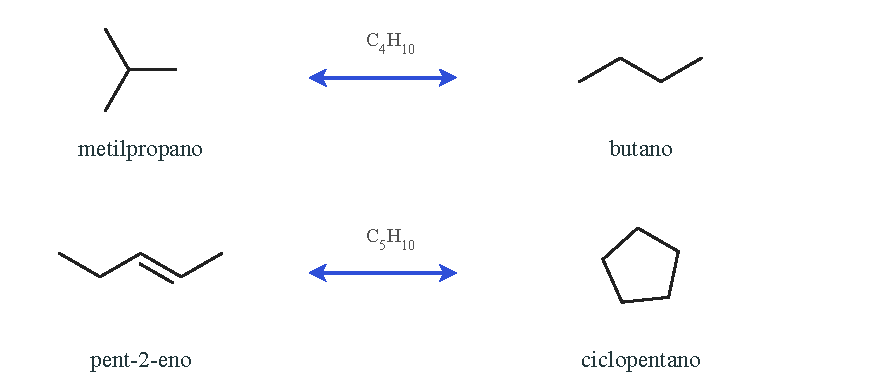
\includegraphics[width=0.70\linewidth]{FigurasSVG/UD9_Quimica_Organica/pdf/UD9_01_isomeria_cadena.pdf}
        \caption{Isomería de cadena}
    \end{figure}

    \item \negsubro{Isomería de posición}. Los compuestos presentan el \textbf{mismo grupo funcional}, pero la posición en la que se encuentra es distinta.

    \begin{figure}[H]
        \centering
        % [FIGURA ORIGINAL] \includegraphics[scale=1]{images/imagesUD9Organica/UD9_Teoria/isomeria_posicion.eps}
        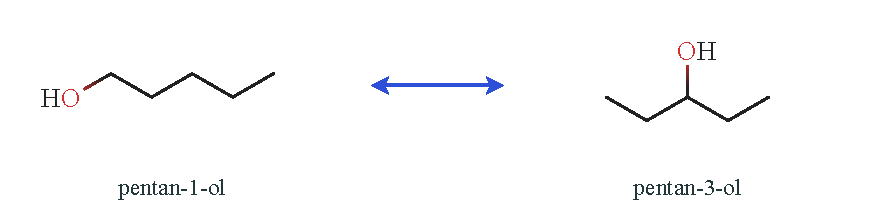
\includegraphics[width=0.70\linewidth]{FigurasSVG/UD9_Quimica_Organica/pdf/UD9_02_isomeria_posicion.pdf}
        \caption{Isomería de posición.}
    \end{figure}

    \item \negsubro{Isomería de función}. Son compuestos que tienen un grupo funcional diferente.

    \begin{figure}[H]
        \centering
        % [FIGURA ORIGINAL] \includegraphics[scale=1]{images/imagesUD9Organica/UD9_Teoria/isomeria_funcion_a.eps}
        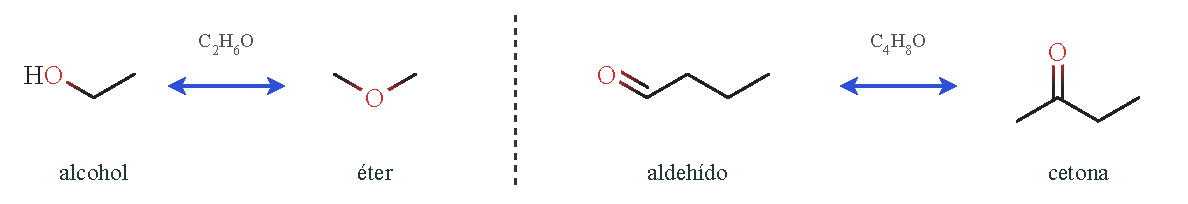
\includegraphics[width=0.95\linewidth]{FigurasSVG/UD9_Quimica_Organica/pdf/UD9_03_isomeria_funcion_a.pdf}
        \caption{Isomería de función. Alcoholes-éteres y aldehídos-cetonas}
    \end{figure}

    \begin{figure}[H]
        \centering
        % [FIGURA ORIGINAL] \includegraphics[scale=1]{images/imagesUD9Organica/UD9_Teoria/isomeria_funcion_b.eps}
        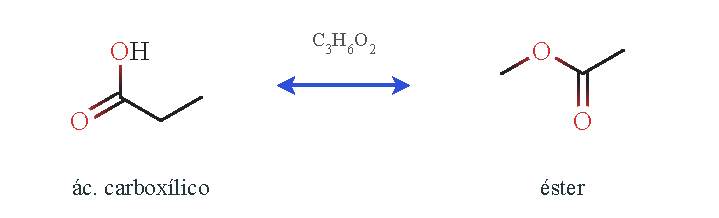
\includegraphics[width=0.57\linewidth]{FigurasSVG/UD9_Quimica_Organica/pdf/UD9_04_isomeria_funcion_b.pdf}
        \caption{Isomería de función. Ácidos carboxílicos-ésteres.}
    \end{figure}

    % \begin{figure}[H]
    %     \centering
    %     \includegraphics[scale=1]{UD9_Teoria/isomeria_funcion.eps}
    % \end{figure}

    Cuando nos pidan un isómero de función de un determinado grupo funcional los podemos asociar de la siguiente manera:

    \begin{enumerate}
        \item Alcoholes \(\iff\) éteres.
        \item Aldehídos \(\iff\) cetonas.
        \item Ácidos carboxílicos \(\iff\) ésteres.
    \end{enumerate}
\end{enumerate}

\subsubsection{Isomería espacial}

\begin{enumerate}[label=\numberballmDarkTeal]
    \item \negsubro{Isomería geométrica}.

    Esta isomería se produce en moléculas rígidas que tengan carbonos con hibridación \(sp^2\) (un alqueno, por ejemplo). Para ello debemos determinar los sustituyentes que están unidos tanto a la izquierda como a la derecha del doble enlace y ver su orientación.

    Antes de ver los tipos de isomería geométrica tenemos que determinar o dar prioridad a los grupos unidos a ese doble enlace. Para asignar la prioridad de los grupos seguiremos la regla de Cahn-Ingold-Prelog (CIP).

    \begin{itemize}
        \item La prioridad se establece según el número atómico del átomo sustituyente, es decir, el átomo unido al doble enlace. Un átomo tiene prioridad sobre otros de número atómico menor. Así pues, el hidrógeno es el que tiene una prioridad más baja.
        % En caso de isótopos, el de mayor masa atómica tiene prioridad.
        \item Si entre dos o más sustituyentes existe coincidencia en el número atómico del átomo unido directamente a la posición cuya prioridad se quiere establecer, se avanza a lo largo de la cadena de cada sustituyente hasta poder asignar un orden de prioridades.
        \begin{figure}[H]
            \centering
            % [FIGURA ORIGINAL] \includegraphics[scale=1]{images/imagesUD9Organica/UD9_Teoria/CIP.eps}
            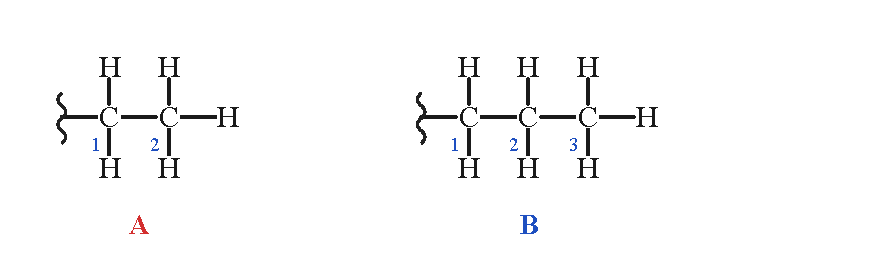
\includegraphics[width=0.70\linewidth]{FigurasSVG/UD9_Quimica_Organica/pdf/UD9_05_reglas_CIP.pdf}
        \end{figure}
    \end{itemize}

    En la siguiente imagen tenemos dos moléculas A y B como sustituyentes. La línea vertical ondulada nos indica donde se encuentra unido al doble enlace. Primero nos fijamos en el primer átomo de carbono (átomo 1) unido al doble enlace: en este caso, en las dos moléculas el átomo unido es el carbono y, por tanto, no podemos asignar una prioridad. Ahora nos centramos en ese átomo de carbono y vemos qué átomos tiene unidos; en ambos casos tiene dos hidrógenos y un átomo de carbono (átomo 2), así que tampoco podemos asignar una prioridad. Ahora nos fijamos en ese átomo 2 de carbono y vemos que el de la molécula A tiene unidos tres átomos de hidrógeno, mientras que el de la molécula B tiene dos átomos de hidrógeno y un átomo de carbono. En este caso sí hay una diferencia y, como la molécula B tiene un átomo con mayor número atómico, la molécula B tendrá prioridad.

    Si tenemos un doble enlace, se considerará ese doble enlace como dos enlaces \ch{C-C}, mientras que si tenemos un grupo carbonilo (\ch{C=O}) se considerará como dos enlaces \ch{C-O}.

    Tenemos dos tipos de isomería:

    \begin{enumerate}[label=\numberballmDarkTeal]
        \item \negsubro{Z o \textit{cis-}}: es aquella en la que los grupos prioritarios se encuentran en el mismo lado.
        \item  \negsubro{E o \textit{trans-}}: es aquella en la que los grupos prioritarios se encuentran en lados opuestos.
        \begin{figure}[H]
            \centering
            % [FIGURA ORIGINAL] \includegraphics[scale=1]{images/imagesUD9Organica/UD9_Teoria/cis_trans.eps}
            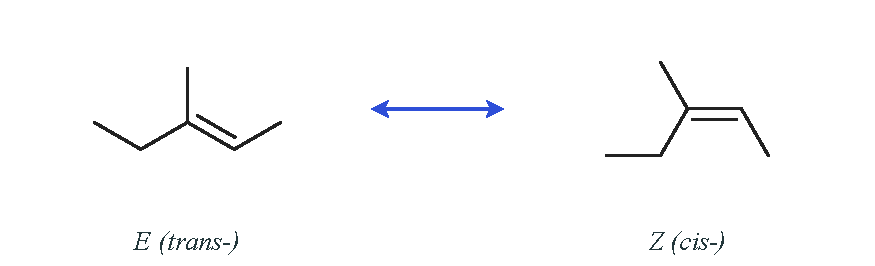
\includegraphics[width=0.70\linewidth]{FigurasSVG/UD9_Quimica_Organica/pdf/UD9_06_isomeria_cis_trans.pdf}
            \caption{Isomería Z/E (cis/trans)}
        \end{figure}
    \end{enumerate}

    Hoy en día, la nomenclatura \textit{cis-} / \textit{trans-} se usa más cuando esos grupos prioritarios son los mismos.

    \item \negsubro{Estereoisomería}. Este tipo de isomería espacial se da en compuestos que tengan un carbono \textbf{estereogénico} o centro \textbf{quiral}, que es aquel que tiene sus 4 sustituyentes diferentes. Estos compuestos se dicen que son compuestos \textbf{quirales}.

    \begin{figure}[H]
        \centering
        % [FIGURA ORIGINAL] \includegraphics[scale=1]{images/imagesUD9Organica/UD9_Teoria/quiralidad.eps}
        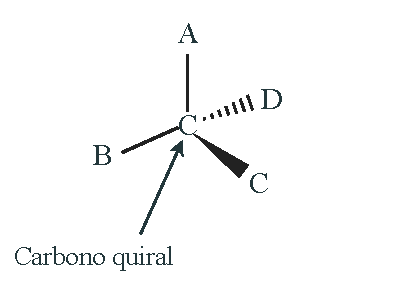
\includegraphics[width=0.33\linewidth]{FigurasSVG/UD9_Quimica_Organica/pdf/UD9_07_carbono_quiral.pdf}
        \caption{Carbono quiral.}
    \end{figure}

    En esta figura, tenemos un compuesto con un carbono quiral, siendo A, B, C y D cuatro sustituyentes distintos entre sí.

    Cuando tenemos un centro quiral, podemos tener dos isómeros llamados \textbf{estereoisómeros} que son el isómero \rectus{} (rectus) y el isómero \sinister{} (sinister). Para determinar si tenemos el isómero \rectus{} o el isómero \sinister{} debemos seguir las siguientes reglas:

    \begin{itemize}
        \item Primero asignamos la prioridad de cada átomo siguiendo las reglas CIP vistas anteriormente.
        \item El de menor prioridad lo situamos lo más alejado de nosotros, es decir, lo ponemos hacia dentro del plano (normalmente es el hidrógeno).
        \item Numeramos los sustituyentes según su prioridad. Al de mayor prioridad le pondremos el 1, al siguiente el 2 y el 3 será el que tenga menor prioridad, sin contar el grupo que hemos situado hacia dentro del plano.
        \item Luego unimos el grupo 1 y el grupo 3 pasando por el grupo 2. Si la dirección descrita sigue el sentido de las agujas del reloj, diremos que tenemos el isómero \rectus{}, mientras que si la dirección sigue el sentido contrario a las agujas del reloj, diremos que es el \sinister{}.
    \end{itemize}

    \begin{figure}[H]
        \centering
        % [FIGURA ORIGINAL] \includegraphics[scale=1]{images/imagesUD9Organica/UD9_Teoria/R_S.eps}
        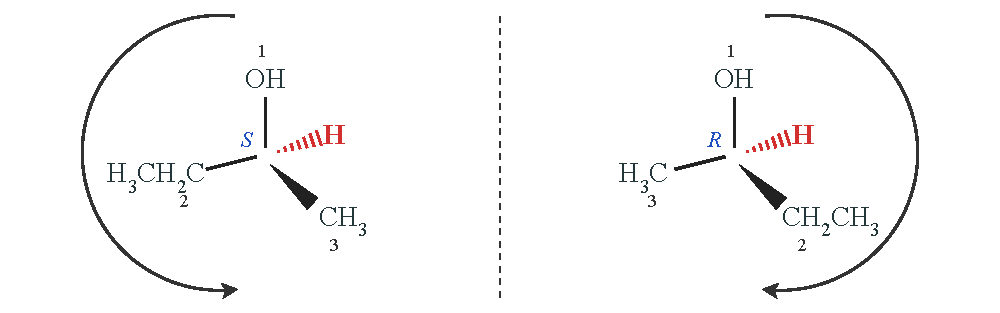
\includegraphics[width=0.80\linewidth]{FigurasSVG/UD9_Quimica_Organica/pdf/UD9_08_configuracion_R_S.pdf}
        \caption{Obtención de la configuración \rectus y \sinister}
    \end{figure}

    Los isómeros \rectus y \sinister diremos que son \textbf{enantiómeros} y son imágenes especulares, es decir, no son superponibles.

    \begin{figure}[H]
        \centering
        % [FIGURA ORIGINAL] \includegraphics[scale=0.5]{images/imagesUD9Organica/UD9_Teoria/imagen_especular.png}
        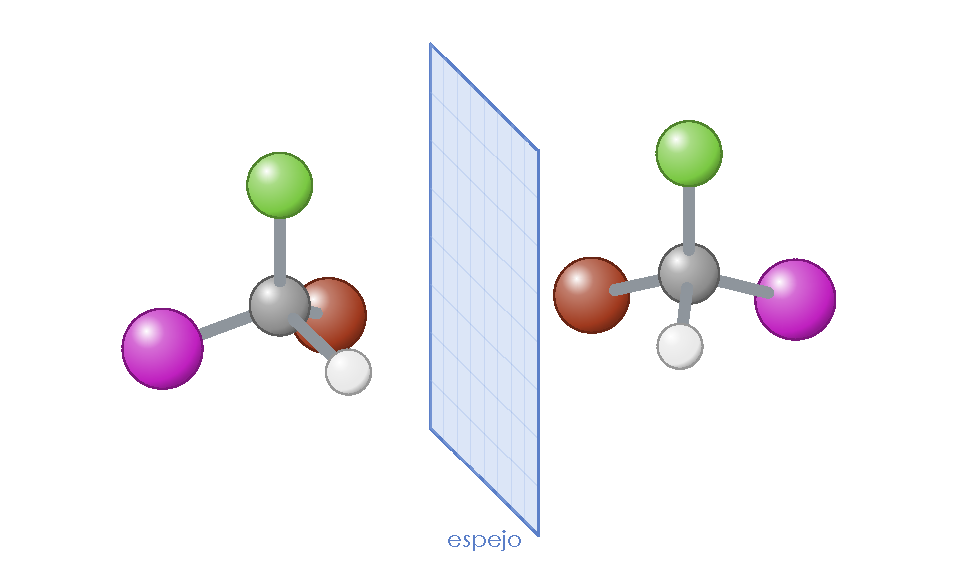
\includegraphics[width=0.6\linewidth]{FigurasSVG/UD9_Quimica_Organica/pdf/UD9_09_imagen_especular.pdf}
        \caption{Imágenes especulares de un compuesto.}
    \end{figure}
\end{enumerate}


\section{Reactividad de los compuestos orgánicos}

En una reacción orgánica, necesitaremos uno o varios compuestos orgánicos, así como una serie de reactivos que ayudarán a que se produzca esa reacción química para formar el producto deseado. Como en toda reacción química, se debe producir primero la ruptura de una serie de enlaces y posteriormente la formación de unos nuevos enlaces.

% \marcador{Breve introducción}

\subsection{Tipos de ruptura de los enlaces}

Tenemos dos tipos de ruptura:

\begin{enumerate}[label=\numberballmDarkTeal]
    \item \negsubro{Ruptura homolítica}: cada átomo que forma el enlace se lleva un electrón (el electrón que había compartido) formando dos radicales. Un radical es una especie que tiene un electrón solitario.
    \begin{figure}[H]
        \centering
        % [FIGURA ORIGINAL] \includegraphics[scale=1]{images/imagesUD9Organica/UD9_Teoria/homolitica.eps}
        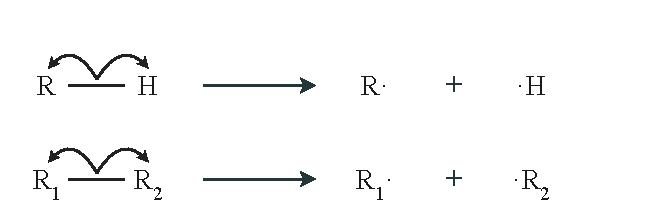
\includegraphics[width=0.53\linewidth]{FigurasSVG/UD9_Quimica_Organica/pdf/UD9_10_ruptura_homolitica.pdf}
    \end{figure}
    \item \negsubro{Ruptura heterolítica}: en este caso, el átomo más electronegativo se lleva los dos electrones del enlace, formando así un anión y un catión. Cuando el catión formado es un compuesto orgánico se llama \textbf{carbocatión}, y si es un anión, \textbf{carbanión}.
    \begin{figure}[H]
        \centering
        % [FIGURA ORIGINAL] \includegraphics[scale=1]{images/imagesUD9Organica/UD9_Teoria/heterolitica.eps}
        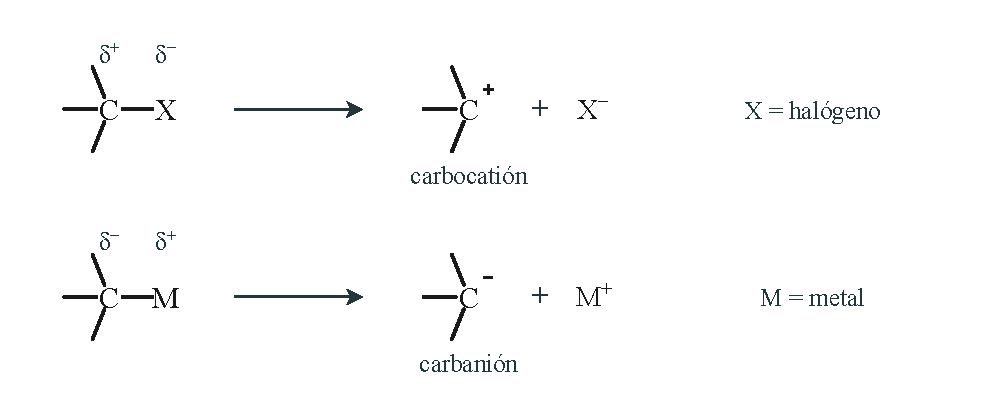
\includegraphics[width=0.80\linewidth]{FigurasSVG/UD9_Quimica_Organica/pdf/UD9_11_ruptura_heterolitica.pdf}
    \end{figure}
\end{enumerate}

\subsection{Tipos de reactivos: nucleófilos y electrófilos}

Tenemos dos tipos de reactivos principalmente:

\begin{enumerate}[label=\numberballmDarkTeal]
    \item \negsubro{Nucleófilos} (\ch{Nu-}). Son aquellos que contienen átomos que pueden ceder electrones y, por tanto, suelen tener carga negativa.

    \item \negsubro{Electrófilos} (\ch{E+}). Son aquellos que contienen átomos que pueden captar electrones.
\end{enumerate}


\begin{table}[H]
    \centering
    \caption{Ejemplos de nucleófilos y electrófilos}
    \vspace{-5pt}
    % --- tabla antigua ---
    % \begin{tblr}{
        % colspec = {| Q[c,m] | Q[c,m] | },
        % row{odd} = {bg=myOrange3!10},
        % row{1} = {bg=myOrange3!90,fg=white,font=\bfseries}
    % }
        % \hline
        % Reactivos nucleófilos & Reactivos electrófilos \\
        % \hline
        % \ch{H2O} & \ch{H3O+} \\
        % \ch{NH3} & \ch{R-CHO} \\
        % \ch{R-OH} & \ch{BF3} \\
        % \ch{R-NH2} & \ch{R_1-CO-R_2} \\
        % \ch{X-} & \ch{X2} (X = halógeno) \\
        % \ch{CN-} &  \\
        % \ch{OH-} &  \\
        % \ch{RO-} &  \\
        % \ch{R-COO-} &  \\
        % \hline
    % \end{tblr}
    % --- tabla nueva ---
    \begin{tabular}{@{}cc@{}}
        \toprule
        \textbf{Reactivos nucleófilos} & \textbf{Reactivos electrófilos} \\
        \midrule
        \ch{H2O} & \ch{H3O+} \\[3pt]
        \ch{NH3} & \ch{R-CHO} \\[3pt]
        \ch{R-OH} & \ch{BF3} \\[3pt]
        \ch{R-NH2} & \ch{R_1-CO-R_2} \\[3pt]
        \ch{X-} & \ch{X2} (X = halógeno) \\[3pt]
        \ch{CN-} &  \\[3pt]
        \ch{OH-} &  \\[3pt]
        \ch{RO-} &  \\[3pt]
        \ch{R-COO-} &  \\
        \bottomrule
    \end{tabular}
\end{table}


\section{Tipos de reacciones orgánicas}

\begin{enumerate}[label=\numberballmDarkTeal]
    \item \negsubro{Reacciones de sustitución}: Son reacciones en las que se sustituye un elemento por otro.
    \begin{figure}[H]
        \centering
        % [FIGURA ORIGINAL] \includegraphics[scale=1]{images/imagesUD9Organica/UD9_Teoria/sustitucion_general.eps}
        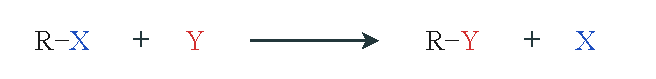
\includegraphics[width=0.53\linewidth]{FigurasSVG/UD9_Quimica_Organica/pdf/UD9_12_sustitucion_general.pdf}
    \end{figure}
    \begin{itemize}
        \item \negsubro{Sustitución radicalaria}: se produce una ruptura homolítica de los enlaces por acción de la luz (se representa por \(h\nu\)). Un ejemplo característico es la halogenación de alcanos, es decir la sustitución de un átomo de H por un halógeno.

        \begin{centeredequation}
            \ch{CH4 + Cl2 ->[\(h\nu\)] CH3Cl + HCl}
        \end{centeredequation}
        \item \negsubro{Sustitución nucleofílica}: se produce cuando un reactivo nucleófilo ataca a un carbono electrófilo. En la mayoría de las ocasiones no tendremos un carbono con la carga positiva, pero sí podemos intuir que el carbocatión se irá formando durante la reacción. Por norma general cuando existe un halógeno unido a un carbono, este se llevará los electrones produciendo una ruptura heterolítica formando así el carbocatión necesario.
        \begin{figure}[H]
            \centering
            % [FIGURA ORIGINAL] \includegraphics[scale=1]{images/imagesUD9Organica/UD9_Teoria/sustitucion_nucleofilica_general.eps}
            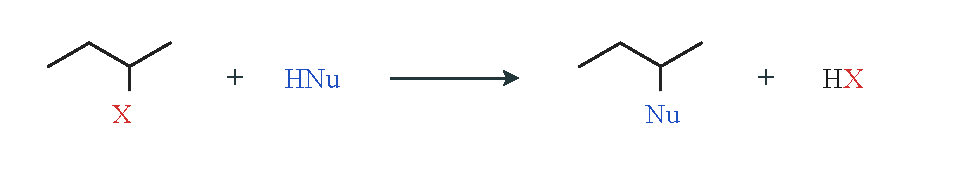
\includegraphics[width=0.77\linewidth]{FigurasSVG/UD9_Quimica_Organica/pdf/UD9_13_sustitucion_nucleofila.pdf}
        \end{figure}
        \begin{itemize}
            \item Sustitución de un halógeno por otro:
            \begin{figure}[H]
                \centering
                % [FIGURA ORIGINAL] \includegraphics[scale=1]{images/imagesUD9Organica/UD9_Teoria/sustitucion_halogeno.eps}
                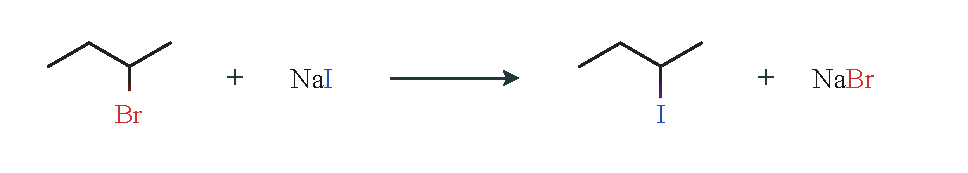
\includegraphics[width=0.77\linewidth]{FigurasSVG/UD9_Quimica_Organica/pdf/UD9_14_sustitucion_halogeno.pdf}
            \end{figure}
            \item Transformación de un derivado halogenado en un alcohol:
            \begin{figure}[H]
                \centering
                % [FIGURA ORIGINAL] \includegraphics[scale=1]{images/imagesUD9Organica/UD9_Teoria/halogeno_y_alcohol.eps}
                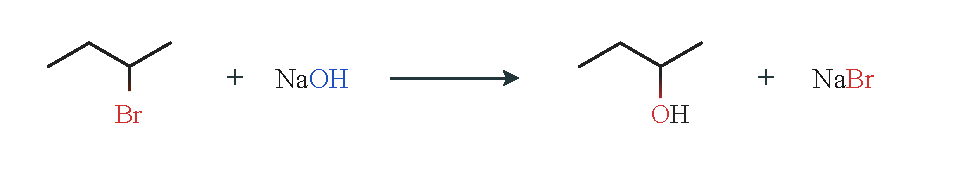
\includegraphics[width=0.77\linewidth]{FigurasSVG/UD9_Quimica_Organica/pdf/UD9_15_halogenuro_a_alcohol.pdf}
            \end{figure}
            \item Transformación de un derivado halogenado en un éter:
            \begin{figure}[H]
                \centering
                % [FIGURA ORIGINAL] \includegraphics[scale=1]{images/imagesUD9Organica/UD9_Teoria/halogeno_y_alcohol_2.eps}
                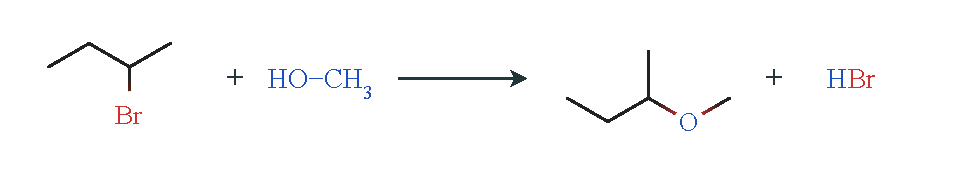
\includegraphics[width=0.77\linewidth]{FigurasSVG/UD9_Quimica_Organica/pdf/UD9_16_halogenuro_a_eter.pdf}
            \end{figure}
            \item Transformación de un derivado halogenado en una amina primaria:
            \begin{figure}[H]
                \centering
                % [FIGURA ORIGINAL] \includegraphics[scale=1]{images/imagesUD9Organica/UD9_Teoria/halogeno_y_amina.eps}
                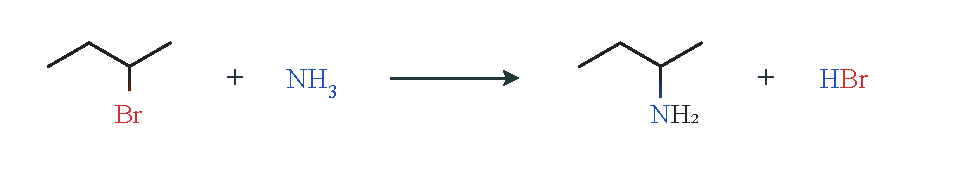
\includegraphics[width=0.77\linewidth]{FigurasSVG/UD9_Quimica_Organica/pdf/UD9_17_halogenuro_a_amina.pdf}
            \end{figure}
            \item Transformación de un derivado halogenado en una amina secundaria o terciaria:

        \end{itemize}
    \end{itemize}

    \item \negsubro{Reacciones de eliminación}: en este tipo de reacciones, se producirá la eliminación de dos átomos formando posteriormente un doble (lo más común) o un triple enlace. En este tipo de reacciones normalmente se requiere una \textbf{base}, a excepción de la deshidratación de alcoholes, que requiere un \textbf{ácido}.
    \begin{figure}[H]
        \centering
        % [FIGURA ORIGINAL] \includegraphics[scale=1]{images/imagesUD9Organica/UD9_Teoria/eliminacion_general.eps}
        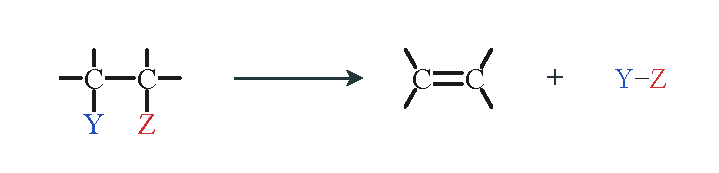
\includegraphics[width=0.57\linewidth]{FigurasSVG/UD9_Quimica_Organica/pdf/UD9_18_eliminacion_general.pdf}
    \end{figure}
    \begin{itemize}
        \item Deshidratación de alcoholes.
        \begin{figure}[H]
            \centering
            % [FIGURA ORIGINAL] \includegraphics[scale=1]{images/imagesUD9Organica/UD9_Teoria/deshidratacion_alcoholes.eps}
            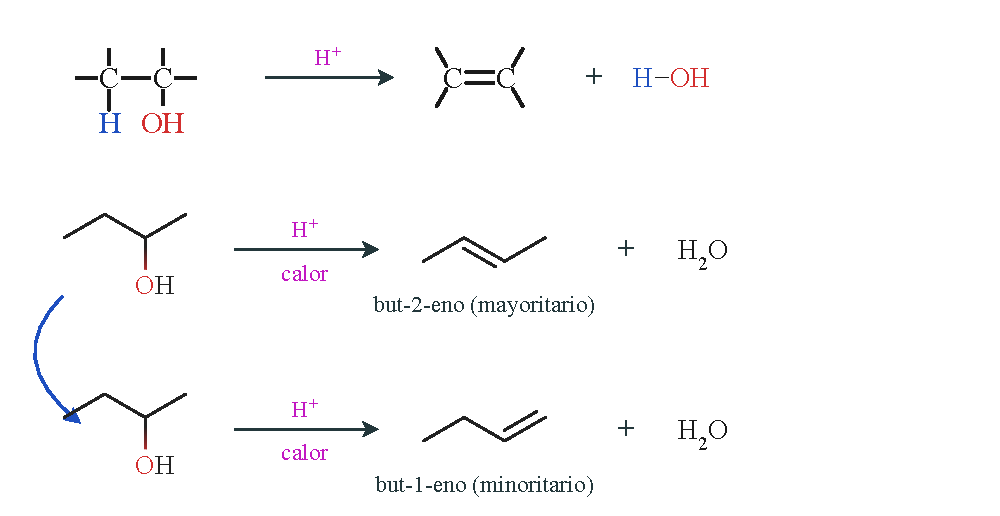
\includegraphics[width=0.80\linewidth]{FigurasSVG/UD9_Quimica_Organica/pdf/UD9_19_deshidratacion_alcoholes.pdf}
        \end{figure}
        \item Deshidrohalogenación de derivados halogenados. X representa el halógeno
        %   \begin{figure}[H]
        %       \centering
        %       \includegraphics[scale=1]{UD9_Teoria/deshalogenacion.eps}
        %   \end{figure}
        \begin{figure}[H]
            \centering
            % [FIGURA ORIGINAL] \includegraphics[scale=1]{images/imagesUD9Organica/UD9_Teoria/deshalogenacion_a.eps}
            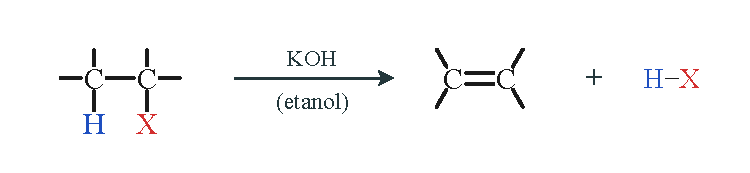
\includegraphics[width=0.60\linewidth]{FigurasSVG/UD9_Quimica_Organica/pdf/UD9_20_deshidrohalogenacion_general.pdf}
        \end{figure}
        \begin{figure}[H]
            \centering
            % [FIGURA ORIGINAL] \includegraphics[scale=1]{images/imagesUD9Organica/UD9_Teoria/deshalogenacion_b.eps}
            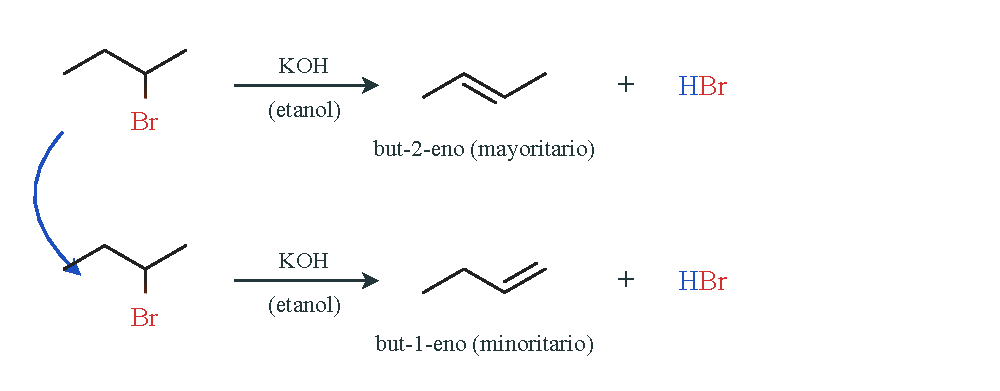
\includegraphics[width=0.80\linewidth]{FigurasSVG/UD9_Quimica_Organica/pdf/UD9_21_deshidrohalogenacion_ejemplo.pdf}
        \end{figure}
    \end{itemize}

        {\normalfont\large\sffamily\bfseries\color{darkblue!80} Formación de alquenos asimétricos}

    Un alqueno asimétrico es aquel que tiene sustituyentes diferentes a ambos lados del doble enlace. Para este tipo de reacciones se sigue la regla de \textbf{Saytzev} que dice que siempre se formará el alqueno más sustituido (por ser más estable). El alqueno más sustituido será aquel que tenga más sustituyentes diferentes al hidrógeno unidos a los carbonos que forman el doble enlace.

    \begin{figure}[H]
        \centering
        % [FIGURA ORIGINAL] \includegraphics[scale=1]{images/imagesUD9Organica/UD9_Teoria/saytzev.eps}
        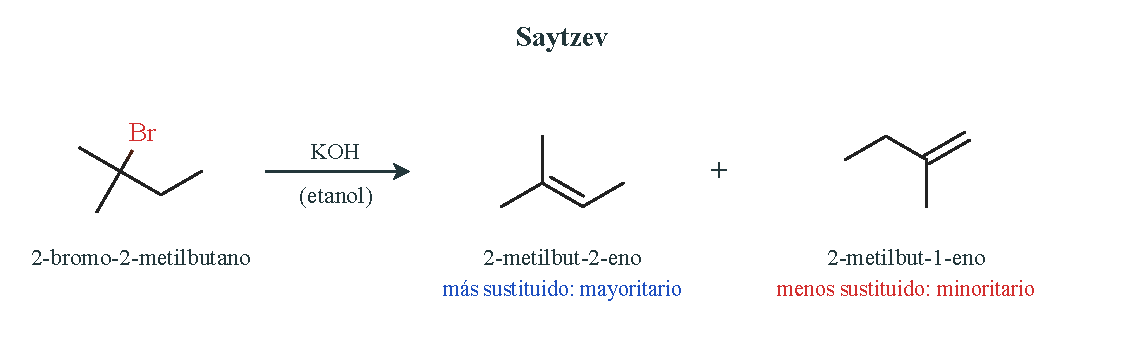
\includegraphics[width=0.90\linewidth]{FigurasSVG/UD9_Quimica_Organica/pdf/UD9_22_regla_saytzev.pdf}
    \end{figure}

    \item \negsubro{Reacciones de adición}: es la adición de un reactivo a un doble o triple enlace.
    \begin{figure}[H]
        \centering
        % [FIGURA ORIGINAL] \includegraphics[scale=1]{images/imagesUD9Organica/UD9_Teoria/adicion_general.eps}
        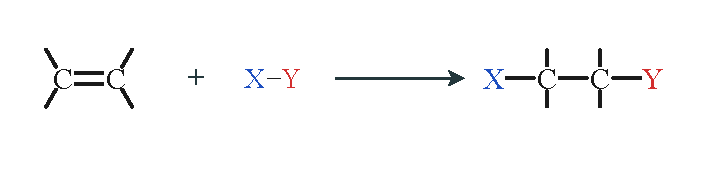
\includegraphics[width=0.57\linewidth]{FigurasSVG/UD9_Quimica_Organica/pdf/UD9_23_adicion_general.pdf}
    \end{figure}
    \begin{itemize}
        \item Hidrogenación de alquenos (adición de \ch{H2}) para dar alcanos:
        \begin{figure}[H]
            \centering
            % [FIGURA ORIGINAL] \includegraphics[scale=1]{images/imagesUD9Organica/UD9_Teoria/adicion_de_hidrogeno.eps}
            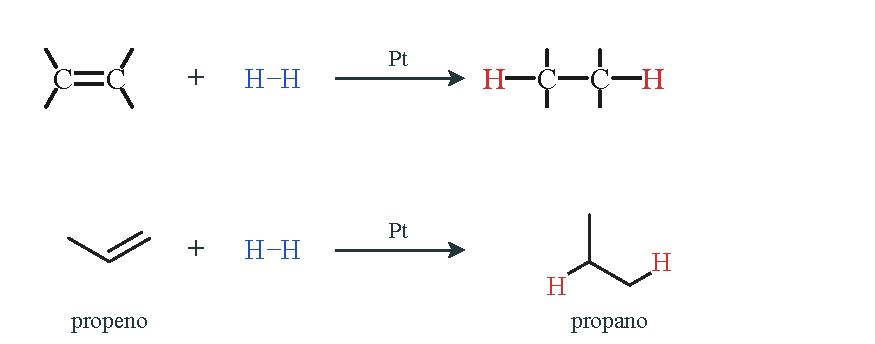
\includegraphics[width=0.70\linewidth]{FigurasSVG/UD9_Quimica_Organica/pdf/UD9_24_adicion_hidrogeno.pdf}
        \end{figure}
        \item Hidratación (adición de \ch{H2O}) de alquenos para dar alcoholes:
        \begin{figure}[H]
            \centering
            % [FIGURA ORIGINAL] \includegraphics[scale=1]{images/imagesUD9Organica/UD9_Teoria/adicion_de_agua.eps}
            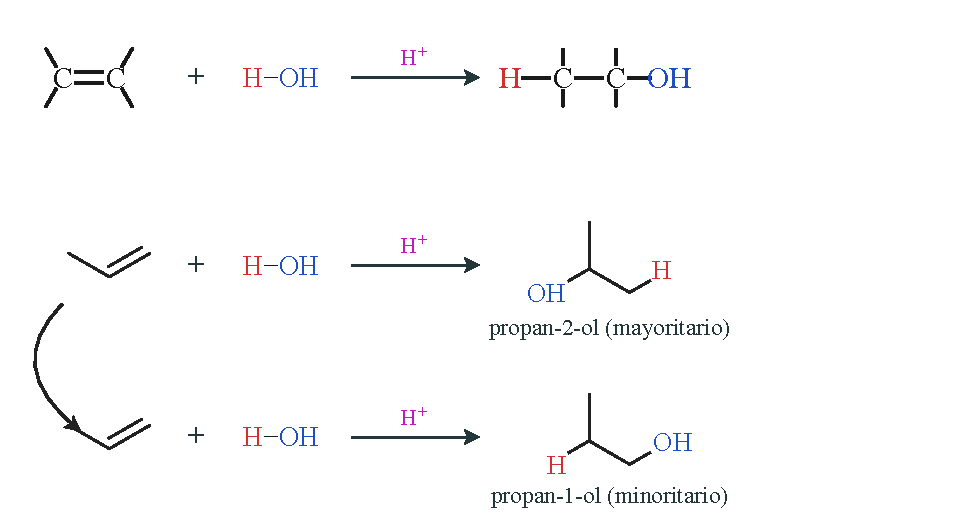
\includegraphics[width=0.77\linewidth]{FigurasSVG/UD9_Quimica_Organica/pdf/UD9_25_adicion_agua.pdf}
        \end{figure}
        \item Adición de haluros de hidrógeno (\ch{HX}) a alquenos para dar derivados halogenados:
        \begin{figure}[H]
            \centering
            % [FIGURA ORIGINAL] \includegraphics[scale=1]{images/imagesUD9Organica/UD9_Teoria/adicion_haluros_hidrogeno.eps}
            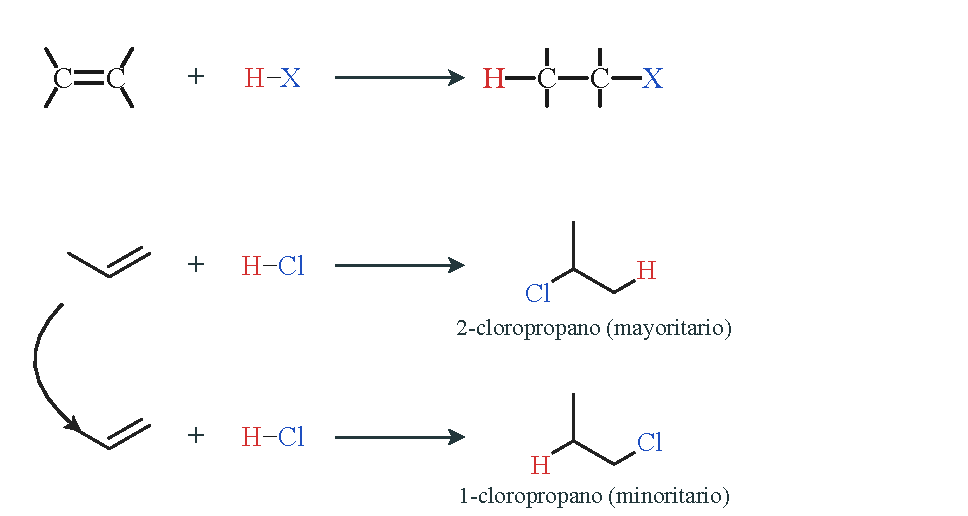
\includegraphics[width=0.77\linewidth]{FigurasSVG/UD9_Quimica_Organica/pdf/UD9_26_adicion_haluros_hidrogeno.pdf}
        \end{figure}
        \item Adición de halógenos (\ch{X2}) a alquenos para dar dihalógenos vecinales:
        \begin{figure}[H]
            \centering
            % [FIGURA ORIGINAL] \includegraphics[scale=1]{images/imagesUD9Organica/UD9_Teoria/adicion_halogenos.eps}
            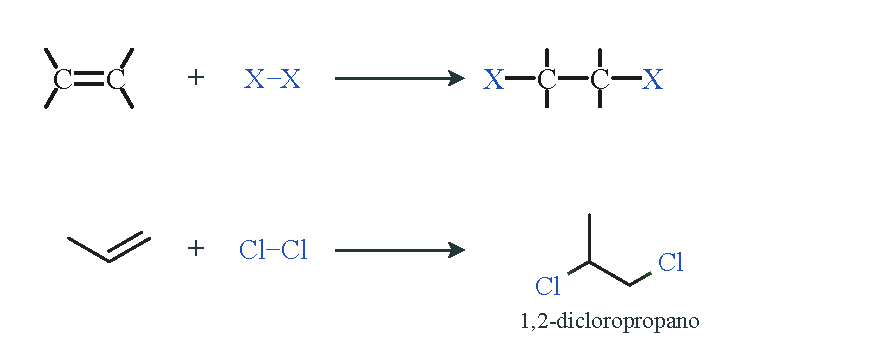
\includegraphics[width=0.70\linewidth]{FigurasSVG/UD9_Quimica_Organica/pdf/UD9_27_adicion_halogenos.pdf}
        \end{figure}
    \end{itemize}

        {\normalfont\large\sffamily\bfseries\color{darkblue!80} Adición en alquenos asimétricos}

    Cuando se produce la adición de un compuesto a un alqueno asimétrico (un alqueno que tienen grupos diferentes tanto a la izquierda como a la derecha del doble enlace), el nucleófilo atacará al átomo de carbono más sustituido mientras que el electrófilo será atacado por el carbono menos sustituido. En el caso de la adición de \ch{HCl} el \ch{Cl-} atacará al carbono de la izquierda mientras que el \ch{H+} se unirá al carbono de la derecha.

    \begin{figure}[H]
        \centering
        % [FIGURA ORIGINAL] \includegraphics[scale=1]{images/imagesUD9Organica/UD9_Teoria/markovnikov.eps}
        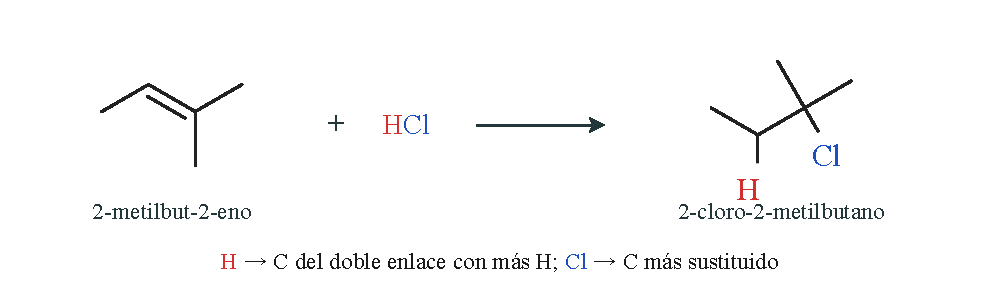
\includegraphics[width=0.80\linewidth]{FigurasSVG/UD9_Quimica_Organica/pdf/UD9_28_regla_markovnikov.pdf}
    \end{figure}

    \item \negsubro{Reacciones de sustitución electrofílica aromática}: son reacciones en las que un electrófilo se ve atacado por un anillo aromático (benceno).
    \begin{figure}[H]
        \centering
        % [FIGURA ORIGINAL] \includegraphics[scale=1]{images/imagesUD9Organica/UD9_Teoria/sustitucion_electrofilica_general.eps}
        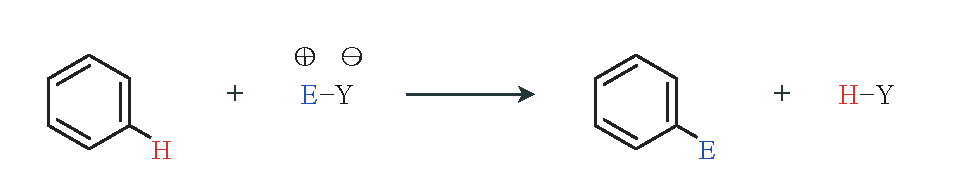
\includegraphics[width=0.77\linewidth]{FigurasSVG/UD9_Quimica_Organica/pdf/UD9_29_sustitucion_electrofila_general.pdf}
    \end{figure}
    Estas reacciones generalmente presentan un catalizador que hace que aumente el carácter electrófilo acelerando así la reacción.
    \begin{itemize}
        \item Halogenación aromática:
        \begin{figure}[H]
            \centering
            % [FIGURA ORIGINAL] \includegraphics[scale=1]{images/imagesUD9Organica/UD9_Teoria/halogenacion_aromatica.eps}
            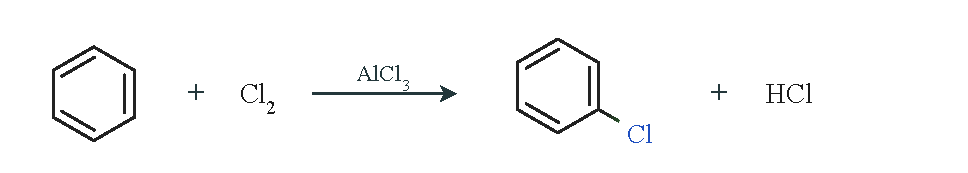
\includegraphics[width=0.77\linewidth]{FigurasSVG/UD9_Quimica_Organica/pdf/UD9_30_halogenacion_aromatica.pdf}
        \end{figure}
        \item Alquilación aromática:
        \begin{figure}[H]
            \centering
            % [FIGURA ORIGINAL] \includegraphics[scale=1]{images/imagesUD9Organica/UD9_Teoria/alquilacion_aromatica.eps}
            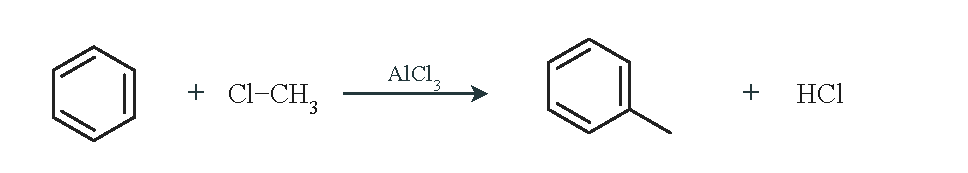
\includegraphics[width=0.77\linewidth]{FigurasSVG/UD9_Quimica_Organica/pdf/UD9_31_alquilacion_aromatica.pdf}
        \end{figure}
        \item Acilación aromática:
        \begin{figure}[H]
            \centering
            % [FIGURA ORIGINAL] \includegraphics[scale=1]{images/imagesUD9Organica/UD9_Teoria/acilacion_aromatica.eps}
            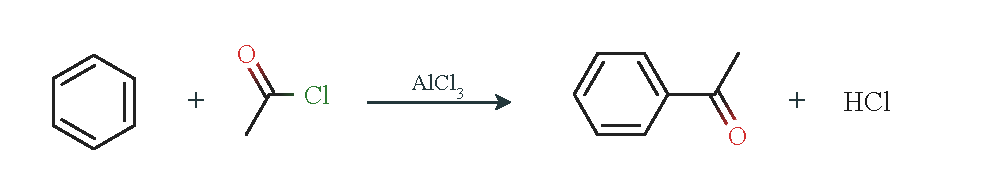
\includegraphics[width=0.80\linewidth]{FigurasSVG/UD9_Quimica_Organica/pdf/UD9_32_acilacion_aromatica.pdf}
        \end{figure}
        \item Nitración aromática:
        \begin{figure}[H]
            \centering
            % [FIGURA ORIGINAL] \includegraphics[scale=1]{images/imagesUD9Organica/UD9_Teoria/nitracion_aromatica.eps}
            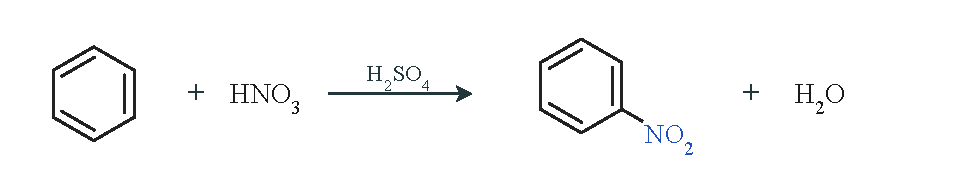
\includegraphics[width=0.77\linewidth]{FigurasSVG/UD9_Quimica_Organica/pdf/UD9_33_nitracion_aromatica.pdf}
        \end{figure}
        \item Sulfonación aromática:
        \begin{figure}[H]
            \centering
            % [FIGURA ORIGINAL] \includegraphics[scale=1]{images/imagesUD9Organica/UD9_Teoria/sulfonacion_aromatica.eps}
            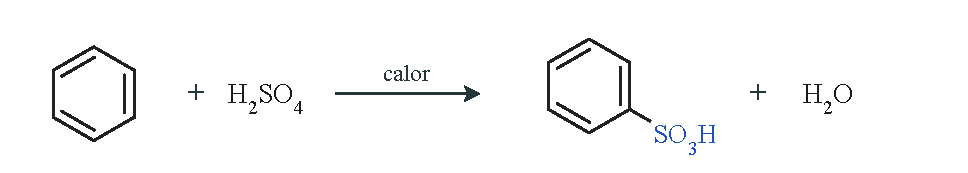
\includegraphics[width=0.77\linewidth]{FigurasSVG/UD9_Quimica_Organica/pdf/UD9_34_sulfonacion_aromatica.pdf}
        \end{figure}
    \end{itemize}
    \item \negsubro{Reacciones de Oxidación-Reducción}: una reacción de oxidación será aquella en la que aumenta el número de átomos de O o disminuye el número de átomos de H. En el caso de la reducción, será cuando aumenta el número de átomos de H o disminuye el número de átomos de O.
    \begin{itemize}
        \item \textbf{Oxidación}: se suelen usar reactivos del tipo \ch{KMnO4}, \ch{K2Cr2O7} o \ch{H2SO4} como oxidantes.

        \item \textbf{Reducción}: se utilizan reactivos del tipo \ch{LiH}, \ch{LiAlH4}, \ch{NaBH4} como reductores.
        \begin{figure}[H]
            \centering
            % [FIGURA ORIGINAL] \includegraphics[scale=1]{images/imagesUD9Organica/UD9_Teoria/oxidacion_reduccion_primarios.eps}
            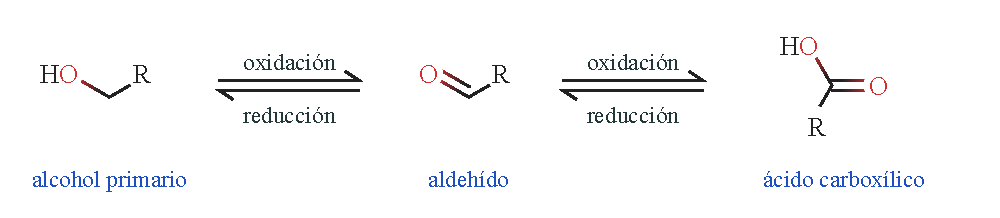
\includegraphics[width=0.80\linewidth]{FigurasSVG/UD9_Quimica_Organica/pdf/UD9_35_oxidacion_alcohol_primario.pdf}
        \end{figure}
        \begin{figure}[H]
            \centering
            % [FIGURA ORIGINAL] \includegraphics[scale=1]{images/imagesUD9Organica/UD9_Teoria/oxidacion_reduccion_secundario.eps}
            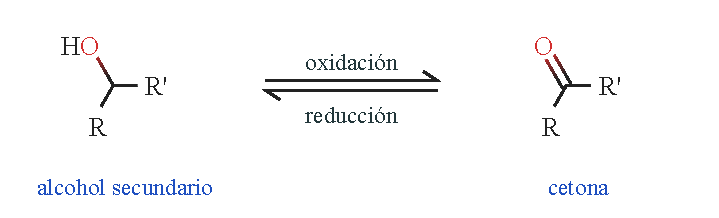
\includegraphics[width=0.57\linewidth]{FigurasSVG/UD9_Quimica_Organica/pdf/UD9_36_oxidacion_alcohol_secundario.pdf}
        \end{figure}
        \begin{figure}[H]
            \centering
            % [FIGURA ORIGINAL] \includegraphics[scale=1]{images/imagesUD9Organica/UD9_Teoria/oxidacion_reduccion_terciario.eps}
            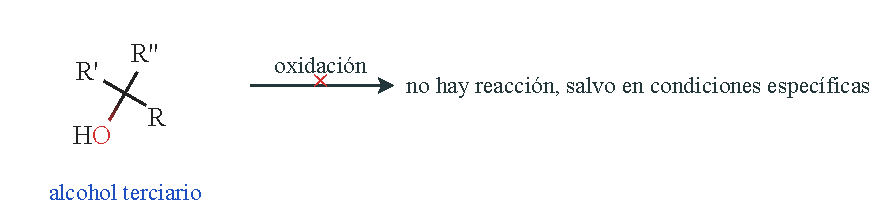
\includegraphics[width=0.70\linewidth]{FigurasSVG/UD9_Quimica_Organica/pdf/UD9_37_oxidacion_alcohol_terciario.pdf}
        \end{figure}
    \end{itemize}
    \item \negsubro{Reacciones de condensación}: son las reacciones en las que dos moléculas orgánicas se unen para formar una molécula de mayor tamaño, perdiéndose una molécula pequeña, generalmente \ch{H2O}.
    \begin{itemize}
        \item Reacción de condensación entre dos moléculas de alcohol para dar un éter.
        \begin{figure}[H]
            \centering
            % [FIGURA ORIGINAL] \includegraphics[scale=1]{images/imagesUD9Organica/UD9_Teoria/condensacion_alcohol_alcohol.eps}
            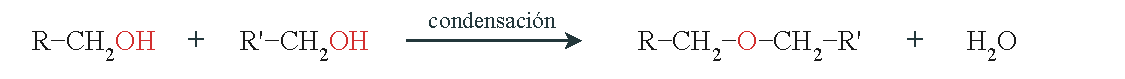
\includegraphics[width=0.90\linewidth]{FigurasSVG/UD9_Quimica_Organica/pdf/UD9_38_condensacion_alcoholes.pdf}
        \end{figure}
        \item Reacción de condensación entre una molécula de ácido carboxílico y un alcohol para formar un éster. A esta reacción se le conoce como \textbf{esterificación}.
        \begin{figure}[H]
            \centering
            % [FIGURA ORIGINAL] \includegraphics[scale=1]{images/imagesUD9Organica/UD9_Teoria/condensacion_acido_alcohol.eps}
            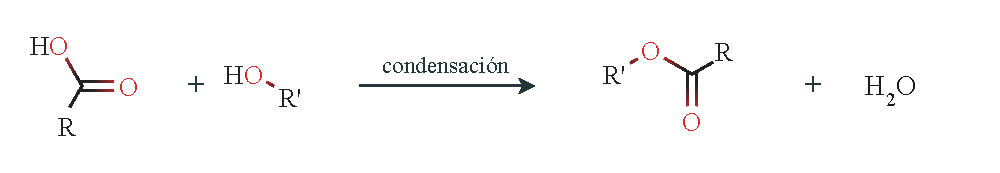
\includegraphics[width=0.80\linewidth]{FigurasSVG/UD9_Quimica_Organica/pdf/UD9_39_condensacion_acido_alcohol.pdf}
        \end{figure}
        \item Reacción entre aminas primarias o secundarias con ácidos carboxílicos para formar amidas.
        \begin{figure}[H]
            \centering
            % [FIGURA ORIGINAL] \includegraphics[scale=1]{images/imagesUD9Organica/UD9_Teoria/condensacion_acido_amina.eps}
            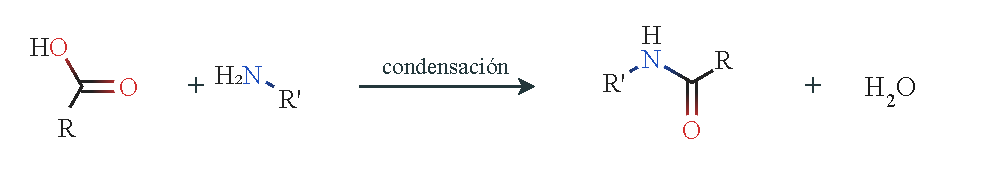
\includegraphics[width=0.80\linewidth]{FigurasSVG/UD9_Quimica_Organica/pdf/UD9_40_condensacion_acido_amina.pdf}
        \end{figure}
    \end{itemize}
    \item \negsubro{Reacciones de hidrólisis}: son reacciones de compuestos orgánicos con agua. Se puede considerar como la reacción opuesta a la reacción de condensación.
    \begin{itemize}
        \item Hidrólisis de éter:
        \begin{figure}[H]
            \centering
            % [FIGURA ORIGINAL] \includegraphics[scale=1]{images/imagesUD9Organica/UD9_Teoria/hidrolisis_eteres.eps}
            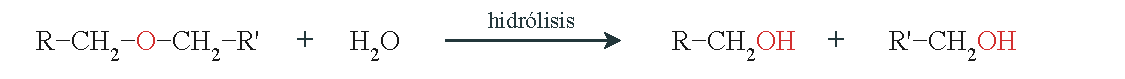
\includegraphics[width=0.90\linewidth]{FigurasSVG/UD9_Quimica_Organica/pdf/UD9_41_hidrolisis_eteres.pdf}
        \end{figure}
        \item Hidrólisis de un éster:
        \begin{figure}[H]
            \centering
            % [FIGURA ORIGINAL] \includegraphics[scale=1]{images/imagesUD9Organica/UD9_Teoria/hidrolisis_ester.eps}
            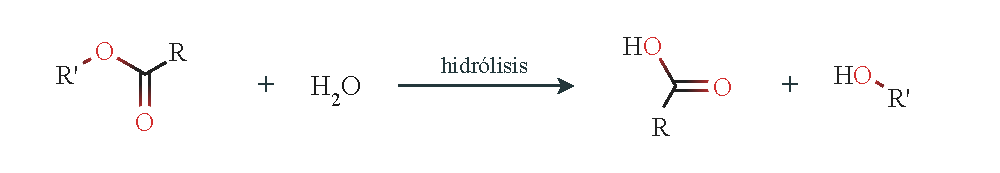
\includegraphics[width=0.80\linewidth]{FigurasSVG/UD9_Quimica_Organica/pdf/UD9_42_hidrolisis_ester.pdf}
        \end{figure}
        \item Hidrólisis de una amida:
        \begin{figure}[H]
            \centering
            % [FIGURA ORIGINAL] \includegraphics[scale=1]{images/imagesUD9Organica/UD9_Teoria/hidrolisis_amida.eps}
            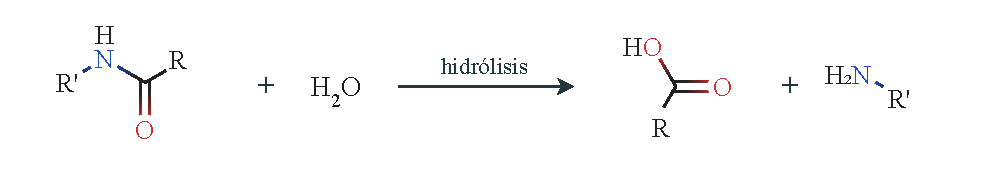
\includegraphics[width=0.80\linewidth]{FigurasSVG/UD9_Quimica_Organica/pdf/UD9_43_hidrolisis_amida.pdf}
        \end{figure}
    \end{itemize}
\end{enumerate}


    \newpage

    %! Author = Profesor
%! Date = 06/06/2024


\section{Ejercicios PAU}

\begin{exerciseEVAU}
    Complete las siguientes reacciones orgánicas:
    \begin{enumerate}[label=\letraminuscula]
        \item \ch{CH2=CH2 + HBr ->}
        \item \ch{CH3CH2CH2OH + H2SO4 ->}
        \item \ch{C4H10 + O2 ->}
        \item \ch{CH3CH2CH2COOH + CH3CH2CH2OH ->}
    \end{enumerate}
\begin{solu}
    
\end{solu}
\end{exerciseEVAU}

\begin{exerciseEVAU}
    De los siguientes pares de compuestos, ¿cuáles son isómeros? ¿Qué tipo de
    isomería presentan?
    \begin{enumerate}[label=\letraminuscula]
        \item
        \begin{figure}[H]
            \centering
            % [FIGURA ORIGINAL] \includegraphics{images/imagesUD9Organica/UD9_Problemas/T9_EvAU_02_a}
            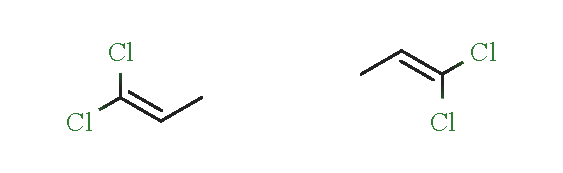
\includegraphics[width=0.45\linewidth]{FigurasSVG/UD9_Quimica_Organica/pdf/UD9_E01_dicloropropeno.pdf}
        \end{figure}
        \item
        \begin{figure}[H]
            \centering
            % [FIGURA ORIGINAL] \includegraphics{images/imagesUD9Organica/UD9_Problemas/T9_EvAU_02_b}
            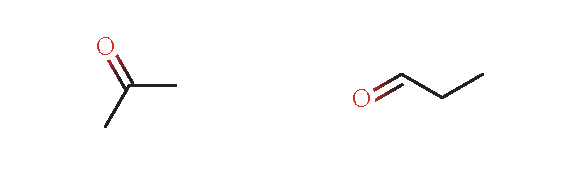
\includegraphics[width=0.45\linewidth]{FigurasSVG/UD9_Quimica_Organica/pdf/UD9_E02_propanona_propanal.pdf}
        \end{figure}
        \item
        \begin{figure}[H]
            \centering
            % [FIGURA ORIGINAL] \includegraphics{images/imagesUD9Organica/UD9_Problemas/T9_EvAU_02_C}
            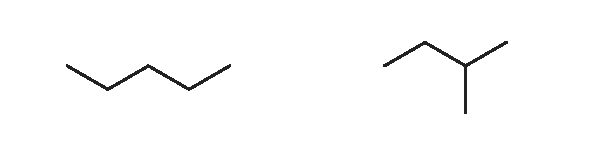
\includegraphics[width=0.47\linewidth]{FigurasSVG/UD9_Quimica_Organica/pdf/UD9_E03_pentano_metilbutano.pdf}
        \end{figure}
        \item
        \begin{figure}[H]
            \centering
            % [FIGURA ORIGINAL] \includegraphics{images/imagesUD9Organica/UD9_Problemas/T9_EvAU_02_D}
            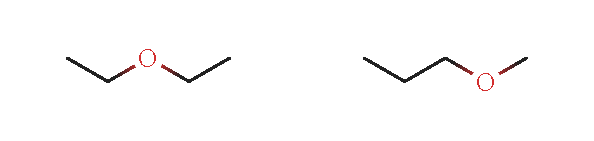
\includegraphics[width=0.47\linewidth]{FigurasSVG/UD9_Quimica_Organica/pdf/UD9_E04_eteres.pdf}
        \end{figure}
    \end{enumerate}

    \begin{solu}
        \begin{enumerate}[label=\letraminuscula]
            \item Ambas estructuras representan la molécula \ch{CH3-CH=CCl2} (1,1-dicloroprop-1-eno), dibujada de dos formas distintas (intercambiando las posiciones del \ch{H} y del \ch{CH3} sobre el carbono no clorado). Como el otro carbono del doble enlace lleva \textbf{dos sustituyentes iguales} (\ch{Cl} y \ch{Cl}), no existe posibilidad de isomería geométrica cis-trans en esta molécula: ambos dibujos son la \textbf{misma sustancia}, no son isómeros.

            \item La primera estructura es la propanona (acetona), \ch{CH3-CO-CH3}, y la segunda es el propanal, \ch{CH3-CH2-CHO}. Ambas tienen la misma fórmula molecular \ch{C3H6O} pero distinto grupo funcional (cetona frente a aldehído), por lo que son \textbf{isómeros de función}.

            \item La primera estructura es el pentano, \ch{CH3-CH2-CH2-CH2-CH3}, y la segunda es el 2-metilbutano, \ch{CH3-CH(CH3)-CH2-CH3}. Ambas responden a la fórmula molecular \ch{C5H12}: la primera es una cadena lineal y la segunda ramificada, por lo que son \textbf{isómeros de cadena}.

            \item La primera estructura es el dietil éter (etoxietano), \ch{CH3-CH2-O-CH2-CH3}, y la segunda es el metil propil éter (1-metoxipropano), \ch{CH3-O-CH2-CH2-CH3}. Ambas tienen fórmula molecular \ch{C4H10O} y el mismo grupo funcional (éter), pero el oxígeno ocupa una posición distinta de la cadena carbonada, por lo que son \textbf{isómeros de posición}.
        \end{enumerate}
    \end{solu}
\end{exerciseEVAU}

\begin{exerciseEVAU}
    Indique el nombre de cada grupo funcional en las siguientes moléculas.

    \begin{enumerate}[label=\letraminuscula]

    \item
    \begin{figure}[H]
        \centering
        % [FIGURA ORIGINAL] \includegraphics{images/imagesUD9Organica/UD9_Problemas/T9_EvAU_03_a}
        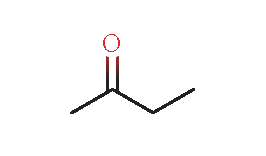
\includegraphics[width=0.21\linewidth]{FigurasSVG/UD9_Quimica_Organica/pdf/UD9_E05_butanona.pdf}
    \end{figure}
    \begin{figure}[H]
        \centering
        % [FIGURA ORIGINAL] \includegraphics{images/imagesUD9Organica/UD9_Problemas/T9_EvAU_03_b}
        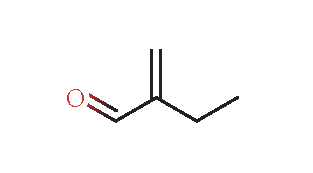
\includegraphics[width=0.25\linewidth]{FigurasSVG/UD9_Quimica_Organica/pdf/UD9_E06_aldehido_insaturado.pdf}
    \end{figure}

    \item \ch{HOOC-CH2-CH2-CHNH-CH3}

    \item
    \begin{figure}[H]
        \centering
        % [FIGURA ORIGINAL] \includegraphics{images/imagesUD9Organica/UD9_Problemas/T9_EvAU_03_d}
        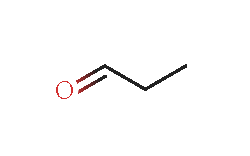
\includegraphics[width=0.20\linewidth]{FigurasSVG/UD9_Quimica_Organica/pdf/UD9_E07_propanal.pdf}
    \end{figure}
    \end{enumerate}
    \begin{solu}
        \begin{enumerate}[label=\letraminuscula]
            \item La primera estructura es el \ch{CH3-CH2-CO-CH3} (butan-2-ona): el grupo carbonilo está unido a dos átomos de carbono, por lo que se trata de una \textbf{cetona}. La segunda estructura representa una cadena carbonada con un grupo \ch{-CHO} terminal (\textbf{aldehído}) combinada con un doble enlace \ch{C=C} (\textbf{alqueno}); es decir, un \textbf{aldehído insaturado}.

            \item \(\ch{HOOC-CH2-CH2-CH(NH2)-CH3}\): la molécula presenta dos grupos funcionales: un grupo \ch{-COOH} (\textbf{ácido carboxílico}) en un extremo de la cadena y un grupo \ch{-NH2} (\textbf{amina primaria}) sobre el carbono próximo al otro extremo.

            \item La estructura es \ch{CH3-CH2-CHO} (propanal): el grupo carbonilo está unido a un átomo de H y a un átomo de C, por lo que se trata de un \textbf{aldehído}.
        \end{enumerate}
    \end{solu}
\end{exerciseEVAU}

\begin{exerciseEVAU}
    \begin{enumerate}[label=\letraminuscula]
        \item En los siguientes compuestos, indique qué tipo de hibridación presenta cada carbono:

        \ch{CH3-COOH}  y  \ch{CH3-C~C-CH3}
        \item De los siguientes compuestos, diga si son ópticamente activos y razone su respuesta.

        \ch{CH2OH-CHBr-COOH} Y \ch{CH3CH2-COOH}
    \end{enumerate}

    \begin{solu}
        \begin{enumerate}[label=\letraminuscula]
            \item En \ch{CH3-COOH} (ácido etanoico): el carbono del grupo \ch{CH3} está unido únicamente por enlaces sencillos (a 3 \ch{H} y al otro carbono), por lo que presenta hibridación \(sp^3\); el carbono del grupo \ch{-COOH} forma un doble enlace con el oxígeno (\ch{C=O}) y enlaces sencillos con \ch{-OH} y con \ch{-CH3}, por lo que presenta hibridación \(sp^2\).

            En \ch{CH3-C~C-CH3} (but-2-ino): los dos carbonos de los grupos \ch{CH3} (extremos) tienen hibridación \(sp^3\); los dos carbonos unidos por el triple enlace \ch{C~C} tienen hibridación \(sp\) (cada uno forma un enlace \(\sigma\) con un grupo metilo, un enlace \(\sigma\) con el otro carbono del triple enlace y dos enlaces \(\pi\) perpendiculares entre sí).

            \item \ch{CH2OH-CHBr-COOH} (ácido 3-hidroxi-2-bromopropanoico): el carbono central (\ch{CHBr}) está unido a cuatro sustituyentes distintos: \ch{-CH2OH}, \ch{-Br}, \ch{-COOH} y \ch{-H}. Al tener cuatro grupos diferentes se trata de un \textbf{carbono asimétrico o quiral}, por lo que la molécula es \textbf{ópticamente activa} (presenta dos enantiómeros).

            \ch{CH3-CH2-COOH} (ácido propanoico) no posee ningún carbono unido a cuatro sustituyentes distintos (el \ch{C2} tiene dos \ch{H} iguales), por lo que \textbf{no es ópticamente activo}.
        \end{enumerate}
    \end{solu}
\end{exerciseEVAU}

\begin{exerciseEVAU}
    \begin{enumerate}[label=\letraminuscula]
        \item
        \begin{enumerate}[label=\letraminuscula]
            \item  Dibuje los isómeros geométricos de la molécula

            \ch{CH3-CH2-CH2-CH=CH-CH2-CH2-CH3}

            \item  Dibuje los isómeros geométricos de la molécula

            \ch{CH3-CH2-CH2-COOH}
        \end{enumerate}
        \item
        \begin{enumerate}[label=\letraminuscula]
            \item Escriba un isómero de fórmula molecular C4H10O que presente actividad óptica Escriba un isómero de fórmula molecular \ch{C4H10O} que presente actividad óptica.
            \item
            \item Escriba dos isómeros correspondientes a la fórmula molecular \ch{5H12}
        \end{enumerate}
    \end{enumerate}

    \begin{solu}
        \begin{enumerate}[label=\letraminuscula]
            \item
            \begin{enumerate}[label=\letraminuscula]
                \item El oct-4-eno, \ch{CH3-CH2-CH2-CH=CH-CH2-CH2-CH3}, presenta isomería geométrica porque cada carbono del doble enlace lleva dos sustituyentes distintos (\ch{H} y \ch{CH2-CH2-CH3}):
                \begin{itemize}
                    \item \emph{cis}-oct-4-eno: los dos grupos propilo (\ch{-CH2CH2CH3}) quedan al mismo lado del doble enlace.
                    \item \emph{trans}-oct-4-eno: los dos grupos propilo quedan en lados opuestos del doble enlace.
                \end{itemize}

                \item \ch{CH3-CH2-CH2-COOH} (ácido butanoico) no presenta isomería geométrica, ya que no contiene ningún doble enlace \ch{C=C}: el único doble enlace de la molécula es el \ch{C=O} del grupo carboxilo, que no puede dar lugar a isomería cis-trans.
            \end{enumerate}

            \item
            \begin{enumerate}[label=\letraminuscula]
                \item Butan-2-ol, \ch{CH3-CH(OH)-CH2-CH3}, presenta actividad óptica: el carbono 2 está unido a cuatro sustituyentes distintos (\ch{-OH}, \ch{-CH3}, \ch{-CH2CH3} y \ch{-H}), por lo que es un carbono asimétrico.

                \item Para la fórmula molecular \ch{C5H12} (pentanos), dos isómeros posibles son:
                \begin{itemize}
                    \item Pentano: \ch{CH3-CH2-CH2-CH2-CH3}
                    \item 2-metilbutano: \ch{CH3-CH(CH3)-CH2-CH3}
                \end{itemize}
                (también sería válido el 2,2-dimetilpropano, \ch{C(CH3)4}).
            \end{enumerate}
        \end{enumerate}
    \end{solu}
\end{exerciseEVAU}

\begin{exerciseEVAU}
    \begin{enumerate}[label=\letraminuscula]
        \item Dibuje los isómeros geométricos cis-trans de 3-hexeno.
        \item Escriba todos los isómeros de fórmula molecular \ch{C5H12}.
        \item Escriba el producto resultante de las siguientes reacciones orgánicas:
        \begin{itemize}
            \item \ch{CH3-CH=CH-CH3 + HCl -> }
            \item \ch{CH3-CH2-CH2-CH2-OH + H2SO4 ->}
        \end{itemize}

    \end{enumerate}
    \begin{solu}
        \begin{enumerate}[label=\letraminuscula]
            \item El 3-hexeno, \ch{CH3-CH2-CH=CH-CH2-CH3}, tiene en cada carbono del doble enlace un \ch{H} y un grupo etilo (\ch{-CH2CH3}), sustituyentes distintos, por lo que presenta isomería cis-trans:
            \begin{itemize}
                \item \emph{cis}-3-hexeno: los dos grupos etilo al mismo lado del doble enlace.
                \item \emph{trans}-3-hexeno: los dos grupos etilo en lados opuestos.
            \end{itemize}

            \item Los isómeros de fórmula molecular \ch{C5H12} son tres:
            \begin{itemize}
                \item Pentano: \ch{CH3-CH2-CH2-CH2-CH3}
                \item 2-metilbutano (isopentano): \ch{CH3-CH(CH3)-CH2-CH3}
                \item 2,2-dimetilpropano (neopentano): \ch{C(CH3)4}
            \end{itemize}

            \item
            \begin{itemize}
                \item \ch{CH3-CH=CH-CH3 + HCl -> CH3-CH2-CHCl-CH3}. Es una reacción de adición electrófila de un hidrácido a un alqueno simétrico (but-2-eno); al ser los dos carbonos del doble enlace equivalentes, se obtiene un único producto: 2-clorobutano.

                \item \ch{CH3-CH2-CH2-CH2-OH + H2SO4 ->[Calor] CH3-CH2-CH=CH2 + H2O}. Es una reacción de eliminación (deshidratación intramolecular) del butan-1-ol catalizada por ácido sulfúrico concentrado en caliente, que da lugar al but-1-eno (y agua).
            \end{itemize}
        \end{enumerate}
    \end{solu}
\end{exerciseEVAU}


\begin{exerciseEVAU}
    Indique que tipo de reacción orgánica tiene lugar en cada uno de los siguientes procesos.
    \begin{enumerate}[label=\letraminuscula]
        \item \ch{CH3-CH2-CHO -> CH3-CH2-CH2-OH}
        \item \ch{CH3-CH2-CH2-OH -> CH3-CH=CH2}
        \item \ch{CH3-CH=CH2 - CH3-CH2-CH2-Br }
        \item \ch{CH3-CH2-COOH + CH3-CH2-CH2-OH -> CH3-CH2-COO-CH2-CH2-CH3 }
        \item \ch{CH3-CH2-CH2-OH -> CH3-CH3-CHO}
    \end{enumerate}
    \begin{solu}
        \begin{enumerate}[label=\letraminuscula]
            \item \textbf{Reducción} del propanal (\ch{CH3-CH2-CHO}) a propan-1-ol (\ch{CH3-CH2-CH2-OH}) por adición de hidrógeno al grupo carbonilo.

            \item \textbf{Eliminación} (deshidratación) del propan-1-ol para dar propeno (\ch{CH3-CH=CH2}), con pérdida de una molécula de agua.

            \item \textbf{Adición} electrófila de \ch{HBr} al propeno, que sigue la regla de Markovnikov y da 1-bromopropano como producto mayoritario (\ch{CH3-CH2-CH2-Br}).

            \item \textbf{Sustitución} (esterificación): el ácido propanoico reacciona con el propan-1-ol para dar el propanoato de propilo y agua, catalizada por medio ácido.

            \item \textbf{Oxidación} del propan-1-ol (alcohol primario) a propanal, \ch{CH3-CH2-CHO} (la fórmula del producto en el enunciado contiene una errata, pues debería ser \ch{CH3-CH2-CHO} y no \ch{CH3-CH3-CHO}).
        \end{enumerate}
    \end{solu}
\end{exerciseEVAU}


\begin{exerciseEVAU}
    \textbf{2024}.
    \begin{enumerate}[label=\letraminuscula]
         \item Escriba las fórmulas de un isómero de cadena y otro de posición del siguiente compuesto:

         \ch{CH3–CH=CH–CH2–CH3}.

         \item \item Escriba la fórmula de un isómero de función de la butanona: \ch{CH3–CH2–CO–CH3}

    \end{enumerate}

    \begin{solu}
        \begin{enumerate}[label=\letraminuscula]
            \item El compuesto \ch{CH3-CH=CH-CH2-CH3} es el pent-2-eno (\ch{C5H10}).
            \begin{itemize}
                \item Isómero de \textbf{cadena} (mismo grupo funcional alqueno, distinta ramificación del esqueleto carbonado): 2-metilbut-2-eno, \ch{CH3-C(CH3)=CH-CH3}.
                \item Isómero de \textbf{posición} (mismo esqueleto lineal y mismo grupo funcional, doble enlace en otra posición): pent-1-eno, \ch{CH2=CH-CH2-CH2-CH3}.
            \end{itemize}

            \item La butanona, \ch{CH3-CH2-CO-CH3} (\ch{C4H8O}), es una cetona. Un isómero de función (mismo \ch{C4H8O}, distinto grupo funcional) es el aldehído butanal: \ch{CH3-CH2-CH2-CHO}.
        \end{enumerate}
    \end{solu}
\end{exerciseEVAU}

\begin{exerciseEVAU}
    \begin{enumerate}[label=\letraminuscula]
        \item Escriba las fórmulas de un isómero de cadena y otro de posición del siguiente compuesto:

        \ch{CH3-CH=CH-CH2-CH3}
        \item Escriba la fórmula de un isómero de función de la butanona:
        
        \ch{CH3-CH2-CO-CH3}
    \end{enumerate}
    \begin{solu}

    \end{solu}
\end{exerciseEVAU}

\begin{exerciseEVAU}
    \textbf{2023}. Complete las siguientes reacciones orgánicas:
    \begin{enumerate}[label=\letraminuscula]
    \item \ch{CH3CH2COOH + CH3CH2OH ->}
    \item \ch{CH2=CH2 + Br2 -> }
    \item \ch{C4H10 + O2 -> }
    \item \ch{CH2=CH2 + H2O ->[\( H2SO4 \)]}
    \end{enumerate}
    \begin{solu}
        \begin{enumerate}[label=\letraminuscula]
            \item \ch{CH3-CH2-COOH + CH3-CH2-OH ->[H+] CH3-CH2-COO-CH2-CH3 + H2O}. Es una \textbf{esterificación} (reacción de sustitución) entre el ácido propanoico y el etanol; se obtiene propanoato de etilo y agua.

            \item \ch{CH2=CH2 + Br2 -> CH2Br-CH2Br}. Es una \textbf{adición electrófila} de dibromo al eteno, que da 1,2-dibromoetano.

            \item \ch{C4H10 + 13/2 O2 -> 4CO2 + 5H2O}. Es una reacción de \textbf{combustión} (oxidación total) del butano.

            \item \ch{CH2=CH2 + H2O ->[H2SO4] CH3-CH2-OH}. Es una \textbf{adición electrófila} (hidratación catalizada por ácido) del eteno, que da etanol.
        \end{enumerate}
    \end{solu}
\end{exerciseEVAU}


\begin{exerciseEVAU}
    Escriba la reacción y nombre los productos obtenidos al someter al 1-butanol (butan-1-ol) a un proceso de:

    \begin{enumerate}[label=\letraminuscula]
        \item Combustión.
        \item Un posible producto de oxidación.
        \item Deshidratación.
        \item Reacción con ácido etanoico.
    \end{enumerate}

    \begin{solu}

%        \begin{figure}[H]
%            \centering
%            \includegraphics[scale=.6]{images/imagesUD9Organica/UD9_Problemas/Organica_EvAU_01.png}
%            %\caption{}
%            %\label{fig:}
%        \end{figure}

        \begin{enumerate}[label=\letraminuscula]
            \item Combustión: \ch{CH3-CH2-CH2-CH2-OH + 6O2 -> 4CO2 + 5H2O}. Reacción de oxidación total, muy exotérmica.

            \item Oxidación (suave, con un oxidante como el dicromato): al ser un alcohol primario se oxida primero a aldehído y, si el oxidante es fuerte, a ácido carboxílico. \ch{CH3-CH2-CH2-CH2-OH ->[ [O] ] CH3-CH2-CH2-CHO} (butanal) \ch{->[ [O] ] CH3-CH2-CH2-COOH} (ácido butanoico).

            \item Deshidratación (eliminación intramolecular, medio ácido y calor): \ch{CH3-CH2-CH2-CH2-OH ->[H2SO4, calor] CH3-CH2-CH=CH2 + H2O}, obteniéndose but-1-eno.

            \item Reacción con ácido etanoico (esterificación): \ch{CH3-CH2-CH2-CH2-OH + CH3-COOH ->[H+] CH3-COO-CH2-CH2-CH2-CH3 + H2O}, obteniéndose el etanoato de butilo (un éster) y agua.
        \end{enumerate}
    \end{solu}
\end{exerciseEVAU}

\begin{exerciseEVAU}
    Escriba las fórmulas semidesarrolladas de las siguientes moléculas

    \begin{enumerate}[label=\letraminuscula]
        \item Butan-2-ol.
        \item 3-metil butan-2-ona
        \item ácido prop-2-enoico
        \item 2,5-dimetil hept-3-eno
        \item Justifique qué molécula o moléculas presenta isomería óptica.
    \end{enumerate}

    \begin{solu}

%        \begin{figure}[H]
%            \centering
%            \includegraphics[scale=.6]{images/imagesUD9Organica/UD9_Problemas/Organica_EvAU_02.png}
%            %\caption{}
%            %\label{fig:}
%        \end{figure}

        \begin{enumerate}[label=\letraminuscula]
            \item Butan-2-ol: \ch{CH3-CH(OH)-CH2-CH3}.
            \item 3-metilbutan-2-ona: \ch{CH3-CO-CH(CH3)-CH3}.
            \item Ácido prop-2-enoico (ácido acrílico): \ch{CH2=CH-COOH}.
            \item 2,5-dimetilhept-3-eno: \ch{CH3-CH(CH3)-CH=CH-CH(CH3)-CH2-CH3}.
            \item El butan-2-ol presenta isomería óptica: su \ch{C2} está unido a cuatro grupos distintos (\ch{-OH}, \ch{-CH3}, \ch{-CH2CH3} y \ch{-H}), luego es un carbono asimétrico. El 2,5-dimetilhept-3-eno también es ópticamente activo: su \ch{C5} está unido a cuatro sustituyentes distintos (\ch{-CH3}, \ch{-CH2CH3}, \ch{-H} y el resto de cadena \ch{-CH=CH-CH(CH3)-CH3}). En cambio, la 3-metilbutan-2-ona no es ópticamente activa, pues el \ch{C3} tiene dos grupos \ch{-CH3} idénticos; y el ácido prop-2-enoico tampoco lo es, ya que ninguno de sus carbonos está unido a cuatro sustituyentes distintos.
        \end{enumerate}
    \end{solu}
\end{exerciseEVAU}

\begin{exerciseEVAU}
    Considere el siguiente compuesto: ácido-2-hidroxipropanoico.

    \begin{enumerate}[label=\letraminuscula]
        \item Escriba su fórmula desarrollada y comente la hibridación de los átomos de carbono que componen esa molécula. Indique la posibilidad de enlaces \(\pi\) presentes en la molécula.
        \item ¿Qué tipo de isomería presenta? Justifique su respuesta
    \end{enumerate}

    \begin{solu}

%        \begin{figure}[H]
%            \centering
%            \includegraphics[scale=.6]{images/imagesUD9Organica/UD9_Problemas/Organica_EvAU_04.png}
%            %\caption{}
%            %\label{fig:}
%        \end{figure}

        \begin{enumerate}[label=\letraminuscula]
            \item El ácido 2-hidroxipropanoico (ácido láctico) tiene la fórmula \ch{CH3-CH(OH)-COOH}. El carbono 1 (\ch{-COOH}) forma un doble enlace con un oxígeno y enlaces sencillos con el \ch{-OH} y con el \ch{C2}, por lo que presenta hibridación \(sp^2\); el carbono 2 (\ch{-CH(OH)-}), unido a cuatro átomos por enlaces sencillos (\ch{C1}, \ch{OH}, \ch{CH3} y \ch{H}), presenta hibridación \(sp^3\); el carbono 3 (\ch{-CH3}), unido solo por enlaces sencillos, también es \(sp^3\). El único enlace \(\pi\) de la molécula es el que forma parte del doble enlace \ch{C=O} del grupo carboxilo.

            \item Presenta isomería óptica: el carbono 2 está unido a cuatro sustituyentes distintos (\ch{-OH}, \ch{-COOH}, \ch{-CH3} y \ch{-H}), por lo que es un carbono asimétrico y la molécula tiene dos enantiómeros (ácido D-láctico y ácido L-láctico).
        \end{enumerate}
    \end{solu}
\end{exerciseEVAU}

\begin{exerciseEVAU}
    El ácido propanoico y el etanoato de metilo son compuestos isómeros.

    \begin{enumerate}[label=\letraminuscula]
        \item Escribir sus fórmulas e indicar qué tipo de isomería presentan.
        \item Justifíquese cuál de ellos debe tener un mayor punto de fusión.
    \end{enumerate}

    El butan-1-ol y el etoxietano (dietil éter) son compuestos isómeros cuyos puntos de ebullición son, respectivamente, \qty{117}{\degreeCelsius} y \qty{42.5}{\degreeCelsius}.

    \begin{enumerate}[label=\letraminuscula]
        \item Escribe la fórmula semidesarrollada de ambos compuestos y explica qué tipo de isomería presentan.
        \item ¿Cómo justificarías la diferencia tan significativa de sus temperaturas de ebullición?
    \end{enumerate}

    \begin{solu}

%        \begin{figure}[H]
%            \centering
%            \includegraphics[scale=.6]{images/imagesUD9Organica/UD9_Problemas/Organica_EvAU_05.png}
%            %\caption{}
%            %\label{fig:}
%        \end{figure}

        \begin{enumerate}[label=\letraminuscula]
            \item El ácido propanoico es \ch{CH3-CH2-COOH} y el etanoato de metilo es \ch{CH3-COO-CH3}; ambos responden a la fórmula molecular \ch{C3H6O2} pero tienen distinto grupo funcional (ácido carboxílico frente a éster), por lo que son \textbf{isómeros de función}.

            \item El ácido propanoico tiene un punto de fusión mayor, ya que sus moléculas pueden formar \textbf{enlaces de hidrógeno} entre sí (a través del grupo \ch{-COOH}, muy polar y con \ch{H} unido a \ch{O}), mientras que el éster no puede formar enlaces de hidrógeno entre sus moléculas (no tiene \ch{H} unido directamente a un átomo muy electronegativo), solo presenta fuerzas dipolo-dipolo, más débiles.
        \end{enumerate}

        \begin{enumerate}[label=\letraminuscula]
            \item El butan-1-ol es \ch{CH3-CH2-CH2-CH2-OH} y el etoxietano es \ch{CH3-CH2-O-CH2-CH3}; ambos tienen fórmula molecular \ch{C4H10O} pero distinto grupo funcional (alcohol frente a éter), por lo que son \textbf{isómeros de función}.

            \item El butan-1-ol tiene un punto de ebullición mucho mayor porque sus moléculas están unidas por \textbf{enlaces de hidrógeno} (el grupo \ch{-OH} tiene un \ch{H} unido a un \ch{O} muy electronegativo), que son fuerzas intermoleculares intensas. El éter, al no tener ningún \ch{H} unido directamente al oxígeno, no puede formar enlaces de hidrógeno entre sus moléculas y solo presenta fuerzas dipolo-dipolo débiles, de ahí su punto de ebullición mucho más bajo.
        \end{enumerate}
    \end{solu}
\end{exerciseEVAU}

\begin{exerciseEVAU}
    Dadas las siguientes reacciones orgánicas, indica de qué tipo son y nombra los correspondientes reactivos y productos:

    \begin{enumerate}[label=\letraminuscula]
        \item \ch{CH3-CHBr-CH3 + KOH -> CH3-CH=CH2 + KBr + H2O}
        \item \ch{CH3-CH2-COOH + CH3-OH ->  CH3-CH2-COO-CH3 + H2O}
    \end{enumerate}

    \begin{solu}

%        \begin{figure}[H]
%            \centering
%            \includegraphics[scale=.6]{images/imagesUD9Organica/UD9_Problemas/Organica_EvAU_06.png}
%            %\caption{}
%            %\label{fig:}
%        \end{figure}

        \begin{enumerate}[label=\letraminuscula]
            \item Es una reacción de \textbf{eliminación}: el 2-bromopropano (\ch{CH3-CHBr-CH3}) reacciona con hidróxido de potasio (una base fuerte) y elimina \ch{HBr} para dar propeno (\ch{CH3-CH=CH2}), además de bromuro de potasio y agua.

            \item Es una reacción de \textbf{sustitución (esterificación)}: el ácido propanoico (\ch{CH3-CH2-COOH}) reacciona con metanol (\ch{CH3-OH}) para dar el propanoato de metilo (\ch{CH3-CH2-COO-CH3}) y agua, en medio ácido.
        \end{enumerate}
    \end{solu}
\end{exerciseEVAU}

\begin{exerciseEVAU}
    Escribe las ecuaciones químicas correspondientes a las siguientes reacciones orgánicas, indica de qué tipo son y nombra el producto orgánico obtenido:

    \begin{enumerate}[label=\letraminuscula]
        \item but-1-eno \ch{+ Br2 ->}
        \item \ch{ácido propanoico} \ch{+} metanol \ch{->}
    \end{enumerate}
    \begin{solu}
        \begin{enumerate}[label=\letraminuscula]
            \item \ch{CH2=CH-CH2-CH3 + Br2 -> CH2Br-CHBr-CH2-CH3}. Es una reacción de \textbf{adición electrófila} de dibromo al but-1-eno; el producto orgánico obtenido es el 1,2-dibromobutano.

            \item \ch{CH3-CH2-COOH + CH3-OH ->[H+] CH3-CH2-COO-CH3 + H2O}. Es una reacción de \textbf{sustitución (esterificación)}; el producto orgánico obtenido es el propanoato de metilo.
        \end{enumerate}
    \end{solu}
\end{exerciseEVAU}

\begin{exerciseEVAU}
    De los compuestos orgánicos con fórmula molecular \ch{C5H12O}, fórmula y nombra:
    \begin{enumerate}[label=\letraminuscula]
        \item Dos isómeros de cadena.
        \item Dos isómeros de función.
    \end{enumerate}

    \begin{solu}

%        \begin{figure}[H]
%            \centering
%            \includegraphics[scale=.6]{images/imagesUD9Organica/UD9_Problemas/Organica_EvAU_07.png}
%            %\caption{}
%            %\label{fig:}
%        \end{figure}

        \begin{enumerate}[label=\letraminuscula]
            \item Dos isómeros de cadena, ambos alcoholes con fórmula \ch{C5H12O} (mismo grupo funcional, distinta ramificación):
            \begin{itemize}
                \item Pentan-1-ol: \ch{CH3-CH2-CH2-CH2-CH2-OH}
                \item 2-metilbutan-1-ol: \ch{CH3-CH2-CH(CH3)-CH2-OH}
            \end{itemize}

            \item Dos isómeros de función (mismo \ch{C5H12O}, distinto grupo funcional):
            \begin{itemize}
                \item Pentan-1-ol (alcohol): \ch{CH3-CH2-CH2-CH2-CH2-OH}
                \item Metil butil éter, 1-metoxibutano (éter): \ch{CH3-O-CH2-CH2-CH2-CH3}
            \end{itemize}
        \end{enumerate}
    \end{solu}
\end{exerciseEVAU}

\begin{exerciseEVAU}
    Sea el ácido 2-cloropropanoico.

    \begin{enumerate}[label=\letraminuscula]
        \item Escribe su fórmula semidesarrollada.
        \item Indica la hibridación que presentan los átomos de carbono de su molécula. Existe algún enlace \(\pi\) en la misma?
        \item ¿Es ópticamente activo? En su caso, ¿cuántos isómeros ópticos tiene?
        \item Escribe la reacción de dicho ácido con el etanol y nombra el producto orgánico que se obtiene.
    \end{enumerate}

    \begin{solu}
        \begin{enumerate}[label=\letraminuscula]
            \item \ch{CH3-CHCl-COOH}

            \item El \ch{C1} (\ch{-COOH}) forma un doble enlace con un oxígeno y enlaces sencillos con \ch{-OH} y con \ch{C2}, por lo que tiene hibridación \(sp^2\); el \ch{C2} (\ch{-CHCl-}), unido por enlaces sencillos a \ch{C1}, \ch{Cl}, \ch{CH3} y \ch{H}, tiene hibridación \(sp^3\); el \ch{C3} (\ch{-CH3}) también es \(sp^3\). Existe un único enlace \(\pi\), el que forma parte del doble enlace \ch{C=O} del grupo carboxilo.

            \item Sí, es ópticamente activo: el \ch{C2} está unido a cuatro sustituyentes distintos (\ch{-Cl}, \ch{-COOH}, \ch{-CH3} y \ch{-H}), por lo que es un carbono asimétrico. Al tener un único carbono quiral, la molécula presenta \(2^1 = 2\) isómeros ópticos (un par de enantiómeros).

            \item \ch{CH3-CHCl-COOH + CH3-CH2-OH ->[H+] CH3-CHCl-COO-CH2-CH3 + H2O}. Es una reacción de esterificación (sustitución) que da lugar al 2-cloropropanoato de etilo.
        \end{enumerate}
    \end{solu}

\end{exerciseEVAU}

\begin{exerciseEVAU}
    Completa las siguientes reacciones, nombra los reactivos y productos e indica de que tipo son.

    \begin{enumerate}[label=\letraminuscula]
        \item \chemfig{CH_3-CH=CH_2} \ch{+ HBr ->}
        \item \chemfig{CH_3-CH_2-CH_2-OH} \ch{->[\( H2SO4\quad \Delta \)]}
        \item \chemfig[atom style={scale=0.4}]{*6(-=-=-=-)} \ch{+ HNO3 ->}
    \end{enumerate}

    \begin{solu}

%        \begin{figure}[H]
%            \centering
%            \includegraphics[scale=.6]{images/imagesUD9Organica/UD9_Problemas/Organica_EvAU_08.png}
%            %\caption{}
%            %\label{fig:}
%        \end{figure}

        \begin{enumerate}[label=\letraminuscula]
            \item \ch{CH3-CH=CH2 + HBr -> CH3-CHBr-CH3}. Reacción de \textbf{adición electrófila} del propeno con bromuro de hidrógeno; según la \textbf{regla de Markovnikov}, el \ch{H} se une al carbono con más hidrógenos (\ch{C1}) y el \ch{Br} al carbono más sustituido (\ch{C2}), formándose 2-bromopropano como producto mayoritario.

            \item \ch{CH3-CH2-CH2-OH ->[H2SO4, calor] CH3-CH=CH2 + H2O}. Reacción de \textbf{eliminación} (deshidratación intramolecular) del propan-1-ol, catalizada por ácido sulfúrico en caliente, que da propeno.

            \item \ch{C6H6 + HNO3 ->[H2SO4] C6H5NO2 + H2O}. Reacción de \textbf{sustitución electrófila aromática} (nitración) del benceno, que da nitrobenceno; el ácido sulfúrico actúa como catalizador generando el electrófilo \ch{NO2+}.
        \end{enumerate}
    \end{solu}
\end{exerciseEVAU}

\begin{exerciseEVAU}
    Indica, razonando la respuesta, si las siguientes reacciones orgánicas son de adición, eliminación o sustitución.
    \begin{enumerate}[label=\letraminuscula]
        \item Obtención de alquenos a partir de alcoholes.
        \item Obtención de derivados halogenados a partir de alquenos.
        \item Obtención de un derivado halogenado a partir de un alcano.
    \end{enumerate}

    \begin{solu}

%        \begin{figure}[H]
%            \centering
%            \includegraphics[scale=.6]{images/imagesUD9Organica/UD9_Problemas/Organica_EvAU_09.png}
%            %\caption{}
%            %\label{fig:}
%        \end{figure}

        \begin{enumerate}[label=\letraminuscula]
            \item Es una reacción de \textbf{eliminación}: a partir de un alcohol (\ch{R-CH2-CH2-OH}) se elimina una molécula de agua (el grupo \ch{-OH} y un \ch{H} de un carbono adyacente) formándose un doble enlace \ch{C=C}, por lo que el número de átomos unidos a la cadena disminuye.

            \item Es una reacción de \textbf{adición}: el alqueno, que posee un doble enlace \ch{C=C} rico en electrones, capta el halógeno (\ch{X2}) o el hidrácido (\ch{HX}), rompiéndose el enlace \(\pi\) para formar dos nuevos enlaces \(\sigma\) sencillos; no se pierde ningún átomo, todos se incorporan a la molécula.

            \item Es una reacción de \textbf{sustitución} (halogenación radicalaria): un átomo de hidrógeno del alcano es reemplazado por un átomo de halógeno, normalmente mediante un mecanismo en cadena de radicales libres iniciado por luz o calor.
        \end{enumerate}
    \end{solu}
\end{exerciseEVAU}

\begin{exerciseEVAU}
    Escribe y nombra 3 isómeros que responden a las siguientes fórmulas moleculares, indicando el tipo de isomería que presentan entre ellos: (a) \ch{C6H4Br2}; (b) \ch{C2H2Cl2}
    \vspace*{8pt}

    \begin{solu}

%        \begin{figure}[H]
%            \centering
%            \includegraphics[scale=.6]{images/imagesUD9Organica/UD9_Problemas/Organica_EvAU_10.png}
%            %\caption{}
%            %\label{fig:}
%        \end{figure}

        \begin{enumerate}[label=\letraminuscula]
            \item Para la fórmula molecular \ch{C6H4Br2} (dibromobenceno), tres isómeros posibles son:
            \begin{itemize}
                \item 1,2-dibromobenceno (\emph{orto}-dibromobenceno)
                \item 1,3-dibromobenceno (\emph{meta}-dibromobenceno)
                \item 1,4-dibromobenceno (\emph{para}-dibromobenceno)
            \end{itemize}
            Los tres tienen la misma fórmula molecular y el mismo tipo de sustituyentes, pero los átomos de bromo ocupan posiciones distintas en el anillo aromático, por lo que son \textbf{isómeros de posición}.

            \item Para la fórmula molecular \ch{C2H2Cl2} (dicloroeteno), tres isómeros posibles son:
            \begin{itemize}
                \item 1,1-dicloroeteno: \ch{CH2=CCl2}
                \item \emph{cis}-1,2-dicloroeteno: los dos \ch{Cl} al mismo lado del doble enlace \ch{CHCl=CHCl}
                \item \emph{trans}-1,2-dicloroeteno: los dos \ch{Cl} en lados opuestos del doble enlace \ch{CHCl=CHCl}
            \end{itemize}
            El 1,1-dicloroeteno es \textbf{isómero de posición} respecto de los otros dos (los dos cloros están sobre el mismo carbono en lugar de uno en cada carbono); a su vez, el \emph{cis}- y el \emph{trans}-1,2-dicloroeteno son \textbf{isómeros geométricos (cis-trans)} entre sí, ya que cada carbono del doble enlace lleva un \ch{Cl} y un \ch{H} (sustituyentes distintos).
        \end{enumerate}
    \end{solu}
\end{exerciseEVAU}

\begin{exerciseEVAU}
    Formula el compuesto 2-propenol (propen-2-ol, prop-1-en-2-ol) y responde a las siguientes cuestiones:

    \begin{enumerate}[label=\letraminuscula]
        \item ¿Cuál es la hibridación de los átomos de carbono 2 y 3?
        \item De todos los enlaces de esta molécula, cuál es el enlace más polar?
        Indica, además, un enlace sigma (\(\sigma\)) y un enlace pi (\(\pi\)).
        \item Formula y nombra un isómero de función del propen-2-ol.
    \end{enumerate}

    \begin{solu}
%        \begin{figure}[H]
%            \centering
%            \includegraphics[scale=.6]{images/imagesUD9Organica/UD9_Problemas/Organica_EvAU_11}
%            %\caption{}
%            %\label{fig:}
%        \end{figure}

        El prop-1-en-2-ol (2-propenol) es \ch{CH2=C(OH)-CH3}, numerando \ch{C1}(\ch{=CH2}), \ch{C2}(\ch{=C(OH)-}) y \ch{C3}(\ch{-CH3}).
        \begin{enumerate}[label=\letraminuscula]
            \item El \ch{C2} forma parte del doble enlace \ch{C1=C2} y está unido, además, al grupo \ch{-OH} y al \ch{-CH3}, por lo que presenta hibridación \(sp^2\). El \ch{C3} (\ch{-CH3}) está unido solo por enlaces sencillos, por lo que presenta hibridación \(sp^3\).

            \item El enlace más polar de la molécula es el enlace \ch{O-H} del grupo hidroxilo, ya que es el que presenta mayor diferencia de electronegatividad entre los átomos que lo forman. Un enlace sigma (\(\sigma\)) es, por ejemplo, el enlace \ch{C2-C3}; un enlace pi (\(\pi\)) es el que, junto con un enlace \(\sigma\), forma el doble enlace \ch{C1=C2}.

            \item El prop-1-en-2-ol es el tautómero enólico de la propanona (acetona), \ch{CH3-CO-CH3}, con la que comparte la fórmula molecular \ch{C3H6O} pero presenta un grupo funcional distinto (enol frente a cetona); por tanto, la propanona es un isómero de función del propen-2-ol.
        \end{enumerate}
    \end{solu}
\end{exerciseEVAU}


% \orbital{s} y ahora el p \orbital{p}

%         \begin{figure}[H]
%             \centering
%             \includegraphics[scale=0.5]{  images/imagesUD9Organica/UD9_Problemas/Organica_EvAU_01.png}
%         \end{figure}


% \begin{figure}[H]
%     \centering
%     \includegraphics[scale=0.5]{  images/imagesUD9Organica/UD9_Problemas/Organica_EvAU_02.png}
% \end{figure}

% \begin{figure}[H]
%     \centering
%     \includegraphics[scale=0.5]{  images/imagesUD9Organica/UD9_Problemas/Organica_EvAU_03.png}
% \end{figure}

% \begin{figure}[H]
%     \centering
%     \includegraphics[scale=0.5]{  images/imagesUD9Organica/UD9_Problemas/Organica_EvAU_04.png}
% \end{figure}





    \chapter{Polímeros}

    \vspace*{20pt}

\section{Polímeros o macromoléculas}

\subsection{¿Qué es un polímero?}

Los \textbf{polímeros} son macromoléculas formadas por la unión repetitiva de unidades
más pequeñas denominadas \textbf{monómeros}, enlazadas mediante enlaces covalentes.
Su masa molecular puede alcanzar millones de unidades de masa atómica, por lo que
presentan propiedades muy diferentes a las de las moléculas pequeñas.

La palabra polímero procede del griego \emph{poly} (muchos) y \emph{meros} (partes).

\begin{center}
\[
n\,\mathrm{M}\longrightarrow (\mathrm{M})_n
\]
\end{center}

Donde $M$ representa el monómero y $n$ el grado de polimerización.

\subsection{Estructura}

Las cadenas poliméricas pueden ser muy largas y establecer interacciones entre ellas
(fuerzas de Van der Waals, puentes de hidrógeno o enlaces cruzados). Estas
interacciones son responsables de propiedades como la rigidez, elasticidad o
temperatura de fusión.

\begin{center}
\begin{tabular}{c}
Monómero $\rightarrow$ Cadena polimérica $\rightarrow$ Material\\
CH$_2$=CH$_2$ $\rightarrow$ (-CH$_2$-CH$_2$-)$_n$ $\rightarrow$ Polietileno
\end{tabular}
\end{center}

\subsection{Características generales}

\begin{itemize}
\item Elevada masa molecular.
\item Baja densidad en comparación con los metales.
\item Buenos aislantes eléctricos y térmicos.
\item Gran resistencia química.
\item Facilidad para moldearse.
\end{itemize}

\subsection{Polímeros naturales y sintéticos}

Los polímeros aparecen tanto en la naturaleza como fabricados industrialmente.

\begin{center}
% --- tabla antigua ---
% \begin{tabular}{p{0.42\linewidth}p{0.42\linewidth}}
% \textbf{Naturales} & \textbf{Sintéticos}\\
% \hline
% Celulosa & Polietileno (PE)\\
% Almidón & PVC\\
% Proteínas & Polipropileno (PP)\\
% ADN & PET\\
% Caucho natural & Nailon\\
% \end{tabular}
% --- tabla nueva ---
\begin{tabular}{@{}p{0.42\linewidth}p{0.42\linewidth}@{}}
    \toprule
    \textbf{Naturales} & \textbf{Sintéticos} \\
    \midrule
    Celulosa & Polietileno (PE) \\[3pt]
    Almidón & PVC \\[3pt]
    Proteínas & Polipropileno (PP) \\[3pt]
    ADN & PET \\[3pt]
    Caucho natural & Nailon \\
    \bottomrule
\end{tabular}
\end{center}

\begin{tcolorbox}[title=Recuerda,colback=blue!5,colframe=blue]
Un polímero está formado por un gran número de monómeros unidos mediante enlaces
covalentes. Cuanto mayor es el número de monómeros, mayor suele ser la masa molecular
y mejores son sus propiedades mecánicas.
\end{tcolorbox}

\subsection*{Ejemplo}

El eteno es un monómero. Al unirse miles de moléculas de eteno mediante una reacción
de polimerización se obtiene polietileno:

\[
n\,CH_2=CH_2 \longrightarrow (-CH_2-CH_2-)_n
\]

Este plástico se emplea en bolsas, envases y recipientes.

\begin{figure}[H]
\centering

\begin{tikzpicture}[
>=Latex,
font=\small,
node distance=8mm,
monomer/.style={
draw,
rounded corners,
fill=cyan!20,
minimum width=2.2cm,
minimum height=0.9cm,
align=center
},
polymer/.style={
draw,
rounded corners,
fill=orange!20,
minimum width=10cm,
minimum height=1cm,
align=center
}
]

%%%%%%%%%%%%%%%%%%%%%%%%%%%%%%%%%%%%%%%%%%%%%%%%%%%%%%%%%%%%
% Monómeros
%%%%%%%%%%%%%%%%%%%%%%%%%%%%%%%%%%%%%%%%%%%%%%%%%%%%%%%%%%%%

\node[monomer] (m1) {Monómero};

\node[right=of m1] (plus1) {$+$};

\node[monomer,right=of plus1] (m2) {Monómero};

\node[right=of m2] (plus2) {$+$};

\node[monomer,right=of plus2] (m3) {Monómero};

\node[right=of m3] (dots) {$\cdots$};

%%%%%%%%%%%%%%%%%%%%%%%%%%%%%%%%%%%%%%%%%%%%%%%%%%%%%%%%%%%%
% Flecha
%%%%%%%%%%%%%%%%%%%%%%%%%%%%%%%%%%%%%%%%%%%%%%%%%%%%%%%%%%%%

\draw[->,very thick]
($(m2.south)+(0,-0.2)$)
--
node[right]{\textbf{Polimerización}}
++(0,-1.6);

%%%%%%%%%%%%%%%%%%%%%%%%%%%%%%%%%%%%%%%%%%%%%%%%%%%%%%%%%%%%
% Polímero
%%%%%%%%%%%%%%%%%%%%%%%%%%%%%%%%%%%%%%%%%%%%%%%%%%%%%%%%%%%%

\node[
polymer,
below=2.3cm of m2
] (poly)
{
Monómero -- Monómero -- Monómero -- Monómero -- Monómero -- Monómero
};

%%%%%%%%%%%%%%%%%%%%%%%%%%%%%%%%%%%%%%%%%%%%%%%%%%%%%%%%%%%%
% Texto inferior
%%%%%%%%%%%%%%%%%%%%%%%%%%%%%%%%%%%%%%%%%%%%%%%%%%%%%%%%%%%%

\node[
below=5mm of poly
]
{\textbf{Macromolécula (Polímero)}};

%%%%%%%%%%%%%%%%%%%%%%%%%%%%%%%%%%%%%%%%%%%%%%%%%%%%%%%%%%%%
% Flechas laterales
%%%%%%%%%%%%%%%%%%%%%%%%%%%%%%%%%%%%%%%%%%%%%%%%%%%%%%%%%%%%

\draw[->]
(m1.south)
to[out=-90,in=160]
(poly.west);

\draw[->]
(m3.south)
to[out=-90,in=20]
(poly.east);

%%%%%%%%%%%%%%%%%%%%%%%%%%%%%%%%%%%%%%%%%%%%%%%%%%%%%%%%%%%%

\node[
left=2.2cm of poly,
align=center
]
{Muchos\\monómeros};

\node[
right=2.2cm of poly,
align=center
]
{Cadena\\polimérica};

\end{tikzpicture}

\caption{Formación de un polímero por unión repetitiva de monómeros.}

\end{figure}

%%%%%%%%%%%%%%%%%%%%%%%%%%%%%%%%%%%%%%%%%%%%%%%%%%%%%%%%%%%%
%%%%%%%%%%%%%%%%%%%%% SECCIÓN 2 %%%%%%%%%%%%%%%%%%%%%%%%%%%%%
%%%%%%%%%%%%%%%%%%%%%%%%%%%%%%%%%%%%%%%%%%%%%%%%%%%%%%%%%%%%

\section{Clasificación de los polímeros}

Los polímeros pueden clasificarse atendiendo a diferentes criterios. Esta clasificación permite relacionar su estructura con sus propiedades físicas, químicas y sus aplicaciones industriales.

\begin{center}
\begin{tikzpicture}[
    node distance=10mm,
    every node/.style={
        draw,
        rounded corners,
        align=center,
        font=\small,
        minimum width=3cm
    },
    >={Latex}
]

% Nodo principal
\node (P) {Polímeros};

% Primer nivel
\node[below left=of P, xshift=-20mm] (O) {Según\\su origen};
\node[below=of P, xshift=-8mm] (C) {Según\\su composición};
\node[below right=of P, xshift=20mm] (E) {Según\\su estructura};

% Segundo nivel
\node[below=18mm of C, xshift=18mm] (T)
{Según su\\comportamiento\\frente al calor};

% Flechas
\draw[-Latex] (P) -- (O);
\draw[-Latex] (P) -- (C);
\draw[-Latex] (P) -- (E);
\draw[-Latex] (P) -- (T);

\end{tikzpicture}
\end{center}

\vspace{0.3cm}

%%%%%%%%%%%%%%%%%%%%%%%%%%%%%%%%%%%%%%%%%%%%%%%%%%%%%%%%%%%%%

\subsection{Clasificación según su origen}

Dependiendo de su procedencia, los polímeros pueden ser naturales o sintéticos.

\begin{enumerate}[label=\alph*)]

\item \textbf{Polímeros naturales}

Son aquellos que se encuentran en la naturaleza y son sintetizados por los seres vivos.

Algunos ejemplos son:

\begin{itemize}
\item Celulosa.
\item Almidón.
\item Proteínas.
\item ADN y ARN.
\item Caucho natural.
\end{itemize}

Estos materiales suelen ser biodegradables y desempeñan funciones estructurales o biológicas.

\item \textbf{Polímeros sintéticos}

Se obtienen mediante procesos industriales a partir de derivados del petróleo o, cada vez más, de materias primas renovables.

Los más importantes son:

\begin{itemize}
\item Polietileno (PE).
\item Polipropileno (PP).
\item Policloruro de vinilo (PVC).
\item Poliestireno (PS).
\item PET.
\item Nailon.
\item Teflón (PTFE).
\end{itemize}

Presentan una enorme importancia industrial debido a su bajo coste y facilidad de fabricación.

\end{enumerate}

%%%%%%%%%%%%%%%%%%%%%%%%%%%%%%%%%%%%%%%%%%%%%%%%%%%%%%%%%%%%%

\subsection{Clasificación según su composición}

Según el número de monómeros diferentes que participan en la polimerización, los polímeros pueden clasificarse en:

\begin{description}

\item[Homopolímeros]

Se forman por la repetición de un único tipo de monómero.

Por ejemplo:

\[
n\,CH_2=CH_2
\longrightarrow
(-CH_2-CH_2-)_n
\]

El polietileno es un homopolímero porque toda la cadena está formada por unidades de eteno.

\vspace{0.3cm}

\item[Heteropolímeros o copolímeros]

Se obtienen a partir de dos o más monómeros distintos.

Ejemplos:

\begin{itemize}

\item PET.

\item Nailon 6,6.

\item Resinas epoxi.

\end{itemize}

La combinación de diferentes monómeros permite modificar las propiedades del material final.

\end{description}

%%%%%%%%%%%%%%%%%%%%%%%%%%%%%%%%%%%%%%%%%%%%%%%%%%%%%%%%%%%%%

\subsection{Clasificación según su estructura}

La forma en que se organizan las cadenas poliméricas determina muchas de sus propiedades mecánicas.

\begin{enumerate}[label=\alph*)]

\item \textbf{Polímeros lineales}

Cada monómero se une únicamente a dos monómeros vecinos formando largas cadenas.

Presentan:

\begin{itemize}

\item Mayor flexibilidad.

\item Buena capacidad de deformación.

\item Pueden fundirse con facilidad.

\end{itemize}

Ejemplos:

PEAD, PVC y nailon.

\vspace{0.4cm}

\item \textbf{Polímeros ramificados}

Algunos monómeros se unen a tres o más posiciones formando ramas laterales.

Estas ramas dificultan el empaquetamiento de las cadenas y disminuyen la densidad del material.

Ejemplo:

PEBD.

\vspace{0.4cm}

\item \textbf{Polímeros reticulados}

Las cadenas se encuentran unidas mediante numerosos enlaces covalentes formando una red tridimensional.

Presentan:

\begin{itemize}

\item Gran rigidez.

\item Elevada resistencia térmica.

\item No pueden fundirse.

\end{itemize}

Ejemplos:

\begin{itemize}

\item Baquelita.

\item Resinas epoxi.

\end{itemize}

\end{enumerate}

%%%%%%%%%%%%%%%%%%%%%%%%%%%%%%%%%%%%%%%%%%%%%%%%%%%%%%%%%%%%%

\subsection{Clasificación según su comportamiento frente al calor}

Cuando aumenta la temperatura, los polímeros no responden todos de la misma forma.

\begin{center}
\begin{tabular}{p{3.5cm}p{7.5cm}}
\toprule
\textbf{Tipo} & \textbf{Características} \\
\midrule

Termoplásticos &
Se ablandan al calentarse y recuperan su forma al enfriarse. Pueden reciclarse mediante fusión.\\

\addlinespace

Termoestables &
Durante su fabricación forman enlaces entre cadenas que impiden volver a fundirlos. Son muy resistentes al calor.\\

\addlinespace

Elastómeros &
Presentan una ligera reticulación que les permite deformarse mucho y recuperar posteriormente su forma original.\\

\bottomrule
\end{tabular}
\end{center}

\vspace{0.3cm}

Ejemplos representativos:

\begin{itemize}

\item Termoplásticos: PE, PP, PVC, PET.

\item Termoestables: baquelita, melamina.

\item Elastómeros: caucho natural, neopreno y silicona.

\end{itemize}

%%%%%%%%%%%%%%%%%%%%%%%%%%%%%%%%%%%%%%%%%%%%%%%%%%%%%%%%%%%%%

\begin{tcolorbox}[
title=Recuerda,
colback=blue!5,
colframe=blue!70!black]

La clasificación de un polímero depende de varios criterios al mismo tiempo. Por ejemplo, el PET es un polímero sintético, copolímero, lineal y termoplástico.

\end{tcolorbox}

%%%%%%%%%%%%%%%%%%%%%%%%%%%%%%%%%%%%%%%%%%%%%%%%%%%%%%%%%%%%%

\begin{tcolorbox}[
title=Curiosidad,
colback=green!5,
colframe=green!50!black]

Aunque solemos asociar los polímeros con los plásticos, muchas biomoléculas esenciales para la vida también son polímeros. El ADN, las proteínas y la celulosa son algunos de los ejemplos más importantes.

\end{tcolorbox}

%
\begin{figure}[H]
\centering

\begin{tikzpicture}[
>=Latex,
font=\small,

main/.style={
rectangle,
rounded corners=3pt,
draw=DarkTeal,
very thick,
fill=DarkTeal!18,
minimum width=3.8cm,
minimum height=0.9cm,
align=center,
drop shadow
},

group/.style={
rectangle,
rounded corners=3pt,
draw=blue!70!black,
thick,
fill=blue!10,
minimum width=3.6cm,
minimum height=0.8cm,
align=center,
drop shadow
},

item/.style={
rectangle,
rounded corners=2pt,
draw=gray!70,
fill=gray!8,
minimum width=3.6cm,
minimum height=0.7cm,
align=left
},

line/.style={
-{Latex[length=3mm]},
thick
}
]

%%%%%%%%%%%%%%%%%%%%%%%%%%%%%%%%%%%%%%%%%%%%%%%%%%%%%%%%%%%%
% Nodo principal
%%%%%%%%%%%%%%%%%%%%%%%%%%%%%%%%%%%%%%%%%%%%%%%%%%%%%%%%%%%%

\node[main] (P) {POLÍMEROS};

%%%%%%%%%%%%%%%%%%%%%%%%%%%%%%%%%%%%%%%%%%%%%%%%%%%%%%%%%%%%
% Nivel 2
%%%%%%%%%%%%%%%%%%%%%%%%%%%%%%%%%%%%%%%%%%%%%%%%%%%%%%%%%%%%

\node[group,below left=2cm and 4.8cm of P] (O)
{Según su\\origen};

\node[group,below left=2cm and 1.5cm of P] (C)
{Según su\\composición};

\node[group,below right=2cm and 1.5cm of P] (E)
{Según su\\estructura};

\node[group,below right=2cm and 4.8cm of P] (T)
{Según su\\comportamiento térmico};

%%%%%%%%%%%%%%%%%%%%%%%%%%%%%%%%%%%%%%%%%%%%%%%%%%%%%%%%%%%%

\draw[line](P)--(O);
\draw[line](P)--(C);
\draw[line](P)--(E);
\draw[line](P)--(T);

%%%%%%%%%%%%%%%%%%%%%%%%%%%%%%%%%%%%%%%%%%%%%%%%%%%%%%%%%%%%
% ORIGEN
%%%%%%%%%%%%%%%%%%%%%%%%%%%%%%%%%%%%%%%%%%%%%%%%%%%%%%%%%%%%

\node[item,below=8mm of O]
(O1)
{• Naturales\\
Celulosa, proteínas, ADN, caucho};

\node[item,below=2mm of O1]
(O2)
{• Sintéticos\\
PE, PVC, PET, nailon};

\draw[line](O)--(O1);
\draw[line](O1)--(O2);

%%%%%%%%%%%%%%%%%%%%%%%%%%%%%%%%%%%%%%%%%%%%%%%%%%%%%%%%%%%%
% COMPOSICIÓN
%%%%%%%%%%%%%%%%%%%%%%%%%%%%%%%%%%%%%%%%%%%%%%%%%%%%%%%%%%%%

\node[item,below=8mm of C]
(C1)
{• Homopolímeros\\
Un único monómero};

\node[item,below=2mm of C1]
(C2)
{• Copolímeros\\
Dos o más monómeros};

\draw[line](C)--(C1);
\draw[line](C1)--(C2);

%%%%%%%%%%%%%%%%%%%%%%%%%%%%%%%%%%%%%%%%%%%%%%%%%%%%%%%%%%%%
% ESTRUCTURA
%%%%%%%%%%%%%%%%%%%%%%%%%%%%%%%%%%%%%%%%%%%%%%%%%%%%%%%%%%%%

\node[item,below=8mm of E]
(E1)
{• Lineales};

\node[item,below=2mm of E1]
(E2)
{• Ramificados};

\node[item,below=2mm of E2]
(E3)
{• Reticulados};

\draw[line](E)--(E1);
\draw[line](E1)--(E2);
\draw[line](E2)--(E3);

%%%%%%%%%%%%%%%%%%%%%%%%%%%%%%%%%%%%%%%%%%%%%%%%%%%%%%%%%%%%
% TÉRMICO
%%%%%%%%%%%%%%%%%%%%%%%%%%%%%%%%%%%%%%%%%%%%%%%%%%%%%%%%%%%%

\node[item,below=8mm of T]
(T1)
{• Termoplásticos};

\node[item,below=2mm of T1]
(T2)
{• Termoestables};

\node[item,below=2mm of T2]
(T3)
{• Elastómeros};

\draw[line](T)--(T1);
\draw[line](T1)--(T2);
\draw[line](T2)--(T3);

%%%%%%%%%%%%%%%%%%%%%%%%%%%%%%%%%%%%%%%%%%%%%%%%%%%%%%%%%%%%

\end{tikzpicture}

\caption{Principales criterios de clasificación de los polímeros.}

\end{figure}

%%%%%%%%%%%%%%%%%%%%%%%%%%%%%%%%%%%%%%%%%%%%%%%%%%%%%%%%%%%%
%%%%%%%%%%%%%%%%%%%%%%% SECCIÓN 3 %%%%%%%%%%%%%%%%%%%%%%%%%%%
%%%%%%%%%%%%%%%%%%%%%%%%%%%%%%%%%%%%%%%%%%%%%%%%%%%%%%%%%%%%

\section{Formación de los polímeros}

Los polímeros se obtienen mediante un conjunto de reacciones químicas denominadas
\textbf{reacciones de polimerización}. Durante estas reacciones, un gran número de
moléculas pequeñas (monómeros) se unen mediante enlaces covalentes para formar una
única macromolécula de gran tamaño.

En términos generales, el proceso puede representarse mediante la expresión:

\[
n\,\mathrm{M}\longrightarrow (\mathrm{M})_n
\]

donde:

\begin{itemize}
    \item \(M\) representa el monómero.
    \item \(n\) es el número de monómeros que forman la cadena.
\end{itemize}

Cuanto mayor sea el valor de \(n\), mayor será la longitud de la cadena y, en
general, mejores serán las propiedades mecánicas del polímero.

%%%%%%%%%%%%%%%%%%%%%%%%%%%%%%%%%%%%%%%%%%%%%%%%%%%%%%%%%%%%%

\subsection{Grado de polimerización}

El número de monómeros que forman una cadena recibe el nombre de
\textbf{grado de polimerización} (\(GP\)).

Matemáticamente se define como

\[
GP=\frac{M_{\rm polímero}}{M_{\rm monómero}}
\]

donde

\begin{itemize}
\item \(M_{\rm polímero}\) es la masa molecular media del polímero.
\item \(M_{\rm monómero}\) es la masa molecular del monómero.
\end{itemize}

En los polímeros industriales el grado de polimerización suele variar desde algunos
cientos hasta varios cientos de miles.

\begin{tcolorbox}[
title=Importante,
colback=yellow!8,
colframe=orange!70!black]

Dos muestras del mismo polímero pueden presentar propiedades diferentes si poseen
distintos grados de polimerización. Cuanto mayor es la longitud de las cadenas,
mayor suele ser la resistencia mecánica y la temperatura de reblandecimiento.

\end{tcolorbox}

%%%%%%%%%%%%%%%%%%%%%%%%%%%%%%%%%%%%%%%%%%%%%%%%%%%%%%%%%%%%%

\subsection{Esquema general de formación}

La formación de un polímero puede entenderse como una sucesión de uniones entre
monómeros.

\begin{center}

\begin{tikzpicture}[
    every node/.style={font=\small},
    box/.style={
        draw,
        rounded corners,
        minimum width=2.2cm,
        minimum height=8mm,
        align=center
    },
    node distance=6mm
]

\node[box] (M1) {Monómero};

\node[right=of M1] (plus) {$+$};

\node[box,right=of plus] (M2) {Monómero};

\node[right=of M2] (arrow) {$\Longrightarrow$};

\node[
    box,
    minimum width=3.8cm,
    right=of arrow
] (P) {$-\mathrm{M}-\mathrm{M}-\mathrm{M}-\cdots$};

\end{tikzpicture}

\end{center}

Durante la reacción, cada monómero aporta uno o varios enlaces que permiten su unión
con los monómeros vecinos, originando largas cadenas moleculares.

%%%%%%%%%%%%%%%%%%%%%%%%%%%%%%%%%%%%%%%%%%%%%%%%%%%%%%%%%%%%%

\subsection{Representación}

Un ejemplo sencillo es la formación del polietileno.

\[
\chemfig{CH_2=CH_2}
\qquad
\Longrightarrow
\qquad
\chemleft(
\chemfig{-CH_2-CH_2-}
\chemright)_n
\]

En esta reacción el doble enlace carbono-carbono desaparece y cada molécula de
eteno queda enlazada con las dos moléculas vecinas.

%%%%%%%%%%%%%%%%%%%%%%%%%%%%%%%%%%%%%%%%%%%%%%%%%%%%%%%%%%%%%

\subsection{Factores que influyen en la polimerización}

Las propiedades del polímero obtenido dependen de numerosos factores:

\begin{enumerate}[label=\alph*)]

\item Naturaleza química del monómero.

\item Temperatura de reacción.

\item Presión.

\item Catalizadores empleados.

\item Tiempo de reacción.

\item Presencia de impurezas.

\end{enumerate}

Modificando estas variables es posible obtener materiales con propiedades muy
diferentes a partir del mismo monómero.

%%%%%%%%%%%%%%%%%%%%%%%%%%%%%%%%%%%%%%%%%%%%%%%%%%%%%%%%%%%%%

\subsection{Relación entre estructura y propiedades}

Las propiedades de un polímero dependen no solamente del monómero utilizado, sino
también de cómo se organizan las cadenas.

\begin{center}

\begin{tabular}{p{4cm}p{8.2cm}}

\toprule

\textbf{Característica} & \textbf{Consecuencia} \\

\midrule

Cadenas largas &
Mayor resistencia mecánica. \\

\addlinespace

Mayor ramificación &
Disminuye la densidad y aumenta la flexibilidad. \\

\addlinespace

Mayor reticulación &
Incrementa la rigidez y la resistencia al calor. \\

\addlinespace

Mayor cristalinidad &
Aumenta la dureza y la temperatura de fusión. \\

\bottomrule

\end{tabular}

\end{center}

%%%%%%%%%%%%%%%%%%%%%%%%%%%%%%%%%%%%%%%%%%%%%%%%%%%%%%%%%%%%%

\subsection{Tipos de polimerización}

Dependiendo del mecanismo mediante el cual se unen los monómeros, las reacciones de
polimerización se clasifican en dos grandes grupos:

\begin{center}

\begin{tikzpicture}[
every node/.style={draw,rounded corners,align=center},
node distance=20mm]

\node (A){Polimerización};

\node[below left=of A,minimum width=4cm](B)
{Adición\\No se eliminan moléculas};

\node[below right=of A,minimum width=4cm](C)
{Condensación\\Se elimina una molécula pequeña};

\draw[-latex](A)--(B);

\draw[-latex](A)--(C);

\end{tikzpicture}

\end{center}

En los siguientes apartados se estudiarán con detalle ambos mecanismos de
polimerización y los polímeros más importantes que se obtienen mediante cada uno de
ellos.

%%%%%%%%%%%%%%%%%%%%%%%%%%%%%%%%%%%%%%%%%%%%%%%%%%%%%%%%%%%%%

\begin{tcolorbox}[
title=Recuerda,
colback=blue!5,
colframe=blue!70!black]

La polimerización consiste en unir un gran número de monómeros para formar una
macromolécula. Dependiendo de si durante el proceso se pierde o no una molécula
pequeña, distinguimos entre polimerización por adición y por condensación.

\end{tcolorbox}

%%%%%%%%%%%%%%%%%%%%%%%%%%%%%%%%%%%%%%%%%%%%%%%%%%%%%%%%%%%%
%%%%%%%%%%%%%%%%%%%%%% SECCIÓN 4A %%%%%%%%%%%%%%%%%%%%%%%%%%%
%%%%%%%%%%%%%%% POLIMERIZACIÓN POR ADICIÓN %%%%%%%%%%%%%%%%%%
%%%%%%%%%%%%%%%%%%%%%%%%%%%%%%%%%%%%%%%%%%%%%%%%%%%%%%%%%%%%

\section{Polimerización por adición}

La \textbf{polimerización por adición} es el proceso mediante el cual un gran número
de monómeros insaturados se unen para formar una macromolécula sin que se produzca la
pérdida de ningún átomo o molécula durante la reacción.

Los monómeros utilizados suelen contener un \textbf{doble} o un \textbf{triple enlace}
carbono-carbono. Durante la polimerización estos enlaces múltiples se rompen,
transformándose en enlaces sencillos que permiten la unión sucesiva de los monómeros.

En consecuencia,

\begin{itemize}
\item la masa del polímero es exactamente la suma de las masas de todos los
monómeros que lo forman;
\item no se generan productos secundarios;
\item el polímero conserva la misma composición elemental que el monómero.
\end{itemize}

Este tipo de polimerización es el más utilizado en la fabricación de plásticos de
gran consumo, como el polietileno o el PVC.

%%%%%%%%%%%%%%%%%%%%%%%%%%%%%%%%%%%%%%%%%%%%%%%%%%%%%%%%%%%%

\subsection{Características}

Las principales características de la polimerización por adición son:

\begin{enumerate}[label=\alph*)]

\item Los monómeros presentan enlaces múltiples (\(\mathrm{C=C}\) o
\(\mathrm{C\equiv C}\)).

\item No se desprenden moléculas pequeñas como agua, amoníaco o cloruro de
hidrógeno.

\item Se obtienen generalmente \textbf{homopolímeros}, ya que la cadena está formada
por la repetición del mismo monómero.

\item El proceso suele producir cadenas muy largas con masas moleculares muy
elevadas.

\end{enumerate}

%%%%%%%%%%%%%%%%%%%%%%%%%%%%%%%%%%%%%%%%%%%%%%%%%%%%%%%%%%%%

\subsection{Representación general}

La reacción general puede escribirse como

\[
n\,CH_2=CH-R
\longrightarrow
(-CH_2-CH(R)-)_n
\]

donde \(R\) representa cualquier átomo o grupo de átomos unido al doble enlace.

Cuando \(R=H\) se obtiene el polietileno; cuando \(R=Cl\), el PVC; y cuando
\(R=C_6H_5\), el poliestireno.

%%%%%%%%%%%%%%%%%%%%%%%%%%%%%%%%%%%%%%%%%%%%%%%%%%%%%%%%%%%%

\subsection{Mecanismo radicalario}

La mayoría de las polimerizaciones por adición tienen lugar mediante un mecanismo
radicalario.

En él intervienen especies químicas muy reactivas denominadas
\textbf{radicales libres}, que poseen un electrón desapareado.

El proceso consta de tres etapas.

%%%%%%%%%%%%%%%%%%%%%%%%%%%%%%%%%%%%%%%%%%%%%%%%%%%%%%%%%%%%

\subsubsection*{1. Iniciación}

La reacción comienza gracias a un iniciador, normalmente un peróxido, que se rompe
por acción del calor o de la luz formando radicales libres.

\[
ROOR
\longrightarrow
2RO\cdot
\]

Estos radicales atacan el doble enlace del primer monómero, originando un nuevo
radical en el extremo de la cadena.

\vspace{0.4cm}

\begin{center}


\begin{tikzpicture}[
    node distance=40mm,
    every node/.style={
        draw,
        rounded corners,
        minimum width=3cm,
        minimum height=8mm
    },
    >={Latex}
]

\node (A) {Iniciador};
\node[right=of A] (C) {Radical libre};

\draw[-Latex,thick] (A.east) -- (C.west);

\end{tikzpicture}


\end{center}

%%%%%%%%%%%%%%%%%%%%%%%%%%%%%%%%%%%%%%%%%%%%%%%%%%%%%%%%%%%%

\subsubsection*{2. Propagación}

El radical formado reacciona con otro monómero, que pasa a formar parte de la cadena.

El nuevo extremo continúa siendo un radical libre, por lo que el proceso puede
repetirse miles de veces.

\[
\cdot CH_2-CH_2
+
CH_2=CH_2
\longrightarrow
CH_2-CH_2-CH_2-CH_2\cdot
\]

Cada nueva incorporación aumenta la longitud de la cadena.

Esta etapa es la responsable del gran tamaño que alcanzan los polímeros.

%%%%%%%%%%%%%%%%%%%%%%%%%%%%%%%%%%%%%%%%%%%%%%%%%%%%%%%%%%%%

\subsubsection*{3. Terminación}

El crecimiento de la cadena finaliza cuando desaparece el radical libre del extremo.

Esto puede suceder de varias formas:

\begin{itemize}

\item Unión de dos cadenas radicalarias.

\item Reacción con una impureza.

\item Transferencia de un átomo de hidrógeno.

\end{itemize}

Una vez terminada la reacción, el polímero ya no puede seguir creciendo.

%%%%%%%%%%%%%%%%%%%%%%%%%%%%%%%%%%%%%%%%%%%%%%%%%%%%%%%%%%%%

\subsection{Esquema del mecanismo}

\begin{center}

\begin{tikzpicture}[node distance=12mm]

\node[draw,rounded corners,minimum width=3cm](A){Iniciación};

\node[right=of A,draw,rounded corners,minimum width=3cm](B){Propagación};

\node[right=of B,draw,rounded corners,minimum width=3cm](C){Terminación};

\draw[-latex,thick](A)--(B);

\draw[-latex,thick](B)--(C);

\end{tikzpicture}

\end{center}

%%%%%%%%%%%%%%%%%%%%%%%%%%%%%%%%%%%%%%%%%%%%%%%%%%%%%%%%%%%%

\subsection{Ejemplo: formación del polietileno}

El polietileno se obtiene por polimerización del eteno.

\[
n\,CH_2=CH_2
\longrightarrow
(-CH_2-CH_2-)_n
\]

Durante la reacción desaparece el doble enlace y cada molécula de eteno queda unida
a las moléculas vecinas mediante enlaces sencillos.

El resultado es una cadena muy larga formada únicamente por átomos de carbono e
hidrógeno.

%%%%%%%%%%%%%%%%%%%%%%%%%%%%%%%%%%%%%%%%%%%%%%%%%%%%%%%%%%%%

\begin{tcolorbox}[
title=Recuerda,
colback=blue!5,
colframe=blue!70!black]

En una polimerización por adición:

\begin{itemize}

\item No se pierde ninguna molécula.

\item Los monómeros poseen dobles o triples enlaces.

\item La masa del polímero es igual a la suma de las masas de los monómeros.

\item Generalmente se obtienen homopolímeros.

\end{itemize}

\end{tcolorbox}

%%%%%%%%%%%%%%%%%%%%%%%%%%%%%%%%%%%%%%%%%%%%%%%%%%%%%%%%%%%%

\begin{tcolorbox}[
title=Curiosidad,
colback=green!5,
colframe=green!60!black]

El polietileno es el plástico más producido del mundo. Cada año se fabrican más de
100 millones de toneladas y se utiliza en bolsas, botellas, envases, tuberías y una
gran variedad de productos cotidianos.

\end{tcolorbox}

%%%%%%%%%%%%%%%%%%%%%%%%%%%%%%%%%%%%%%%%%%%%%%%%%%%%%%%%%%%%
%%%%%%%%%%%%%%%%%%%%%%% SECCIÓN 4B %%%%%%%%%%%%%%%%%%%%%%%%%%
%%%%%%%%%%%% PRINCIPALES POLÍMEROS DE ADICIÓN %%%%%%%%%%%%%%%
%%%%%%%%%%%%%%%%%%%%%%%%%%%%%%%%%%%%%%%%%%%%%%%%%%%%%%%%%%%%

\section{Principales polímeros de adición}

La polimerización por adición permite obtener algunos de los materiales más utilizados
en la actualidad. La mayoría de ellos son termoplásticos, ligeros, resistentes a la
corrosión y fáciles de moldear, lo que explica su enorme importancia industrial.

%%%%%%%%%%%%%%%%%%%%%%%%%%%%%%%%%%%%%%%%%%%%%%%%%%%%%%%%%%%%

\subsection{Polietileno (PE)}

El polietileno es el polímero de mayor producción mundial. Se obtiene por
polimerización del eteno.

\[
n\,CH_2=CH_2
\longrightarrow
(-CH_2-CH_2-)_n
\]

Dependiendo de las condiciones de fabricación pueden obtenerse dos tipos principales:

\begin{itemize}
\item \textbf{PEBD (polietileno de baja densidad):} presenta cadenas muy ramificadas,
es flexible y ligero.
\item \textbf{PEAD (polietileno de alta densidad):} posee cadenas casi lineales,
presentando mayor resistencia mecánica y rigidez.
\end{itemize}

\textbf{Aplicaciones}

\begin{itemize}
\item Bolsas de plástico.
\item Botellas.
\item Envases alimentarios.
\item Tuberías.
\item Aislamiento de cables.
\end{itemize}

%%%%%%%%%%%%%%%%%%%%%%%%%%%%%%%%%%%%%%%%%%%%%%%%%%%%%%%%%%%%

\subsection{Polipropileno (PP)}

Se obtiene mediante la polimerización del propeno.

\[
n\,CH_2=CH-CH_3
\longrightarrow
(-CH_2-CH(CH_3)-)_n
\]

Es un plástico muy ligero, rígido y resistente a numerosos productos químicos.

\textbf{Aplicaciones}

\begin{itemize}
\item Tapones.
\item Envases reutilizables.
\item Material sanitario.
\item Componentes de automóviles.
\item Mobiliario.
\end{itemize}

%%%%%%%%%%%%%%%%%%%%%%%%%%%%%%%%%%%%%%%%%%%%%%%%%%%%%%%%%%%%

\subsection{Policloruro de vinilo (PVC)}

Se obtiene a partir del cloroeteno (cloruro de vinilo).

\[
n\,CH_2=CHCl
\longrightarrow
(-CH_2-CHCl-)_n
\]

La presencia del átomo de cloro aumenta su dureza y resistencia al envejecimiento.

Según los aditivos empleados puede obtenerse un PVC rígido o flexible.

\textbf{Aplicaciones}

\begin{itemize}
\item Tuberías.
\item Ventanas.
\item Aislamiento eléctrico.
\item Tarjetas.
\item Suelos vinílicos.
\end{itemize}

%%%%%%%%%%%%%%%%%%%%%%%%%%%%%%%%%%%%%%%%%%%%%%%%%%%%%%%%%%%%

\subsection{Poliestireno (PS)}

Procede de la polimerización del estireno.

\[
n\,CH_2=CH(C_6H_5)
\longrightarrow
(-CH_2-CH(C_6H_5)-)_n
\]

Es un material rígido y transparente.

Cuando contiene gran cantidad de aire recibe el nombre de
\textbf{poliestireno expandido (EPS)}, conocido comercialmente como
\emph{corcho blanco}.

\textbf{Aplicaciones}

\begin{itemize}
\item Embalajes.
\item Vasos desechables.
\item Bandejas para alimentos.
\item Aislamiento térmico.
\end{itemize}

%%%%%%%%%%%%%%%%%%%%%%%%%%%%%%%%%%%%%%%%%%%%%%%%%%%%%%%%%%%%

\subsection{Politetrafluoroetileno (PTFE)}

El PTFE, conocido comercialmente como \textbf{Teflón}, se obtiene a partir del
tetrafluoroeteno.

\[
n\,CF_2=CF_2
\longrightarrow
(-CF_2-CF_2-)_n
\]

Posee una extraordinaria resistencia química y un coeficiente de rozamiento muy bajo.

\textbf{Aplicaciones}

\begin{itemize}
\item Recubrimientos antiadherentes.
\item Juntas.
\item Válvulas.
\item Material de laboratorio.
\item Industria química.
\end{itemize}

%%%%%%%%%%%%%%%%%%%%%%%%%%%%%%%%%%%%%%%%%%%%%%%%%%%%%%%%%%%%

\subsection{Comparación de los principales polímeros}

\begin{center}

\renewcommand{\arraystretch}{1.3}

\begin{tabular}{p{2.6cm}p{2.9cm}p{3cm}p{4cm}}

\toprule

\textbf{Polímero} &
\textbf{Monómero} &
\textbf{Propiedad destacada} &
\textbf{Aplicaciones} \\

\midrule

Polietileno (PE)

& Eteno

& Flexible y ligero

& Bolsas, botellas, envases \\

\addlinespace

Polipropileno (PP)

& Propeno

& Muy resistente

& Tapones, recipientes, mobiliario \\

\addlinespace

PVC

& Cloroeteno

& Muy resistente al desgaste

& Tuberías, ventanas, cables \\

\addlinespace

Poliestireno (PS)

& Estireno

& Ligero y aislante

& Embalajes y envases \\

\addlinespace

PTFE

& Tetrafluoroeteno

& Antiadherente y resistente

& Sartenes, válvulas y juntas \\

\bottomrule

\end{tabular}

\end{center}

%%%%%%%%%%%%%%%%%%%%%%%%%%%%%%%%%%%%%%%%%%%%%%%%%%%%%%%%%%%%

\subsection{Ventajas de los polímeros de adición}

La enorme difusión de estos materiales se debe a que presentan numerosas ventajas:

\begin{itemize}

\item Baja densidad.

\item Elevada resistencia química.

\item Buenos aislantes eléctricos.

\item Facilidad de fabricación.

\item Bajo coste.

\item Gran variedad de propiedades.

\end{itemize}

No obstante, muchos de ellos son poco biodegradables, por lo que resulta imprescindible
su correcta reutilización y reciclaje.

%%%%%%%%%%%%%%%%%%%%%%%%%%%%%%%%%%%%%%%%%%%%%%%%%%%%%%%%%%%%

\begin{tcolorbox}[
title=Importante,
colback=blue!5,
colframe=blue!70!black]

Todos los polímeros estudiados en esta sección se obtienen mediante
\textbf{polimerización por adición}. En ellos no se elimina ninguna molécula durante
la reacción y la unidad repetitiva conserva todos los átomos del monómero original.

\end{tcolorbox}

%%%%%%%%%%%%%%%%%%%%%%%%%%%%%%%%%%%%%%%%%%%%%%%%%%%%%%%%%%%%

\begin{tcolorbox}[
title=Curiosidad,
colback=green!5,
colframe=green!60!black]

Aunque el Teflón es conocido por su uso en utensilios de cocina, también se emplea en
la industria aeroespacial, en equipos médicos y en componentes electrónicos debido a
su extraordinaria estabilidad química y térmica.

\end{tcolorbox}

%%%%%%%%%%%%%%%%%%%%%%%%%%%%%%%%%%%%%%%%%%%%%%%%%%%%%%%%%%%%
%%%%%%%%%%%%%%%%%%%%%%%% SECCIÓN 5 %%%%%%%%%%%%%%%%%%%%%%%%%%
%%%%%%%%%%%%%% POLIMERIZACIÓN POR CONDENSACIÓN %%%%%%%%%%%%%%
%%%%%%%%%%%%%%%%%%%%%%%%%%%%%%%%%%%%%%%%%%%%%%%%%%%%%%%%%%%%

\section{Polimerización por condensación}

La \textbf{polimerización por condensación} consiste en la unión sucesiva de dos o más
tipos de monómeros mediante reacciones en las que, además del polímero, se forma una
molécula pequeña como agua (\(\mathrm{H_2O}\)), cloruro de hidrógeno
(\(\mathrm{HCl}\)) o metanol (\(\mathrm{CH_3OH}\)).

A diferencia de la polimerización por adición, en este proceso la masa del polímero
\textbf{no coincide} exactamente con la suma de las masas de los monómeros, ya que
parte de la materia se elimina en forma de moléculas pequeñas.

En la mayoría de los casos intervienen monómeros que poseen dos grupos funcionales,
lo que permite que la reacción continúe en ambos extremos de la cadena.

%%%%%%%%%%%%%%%%%%%%%%%%%%%%%%%%%%%%%%%%%%%%%%%%%%%%%%%%%%%%

\subsection{Características}

Los polímeros obtenidos por condensación presentan las siguientes características:

\begin{itemize}

\item Se forman mediante reacciones entre grupos funcionales.

\item Durante la reacción se elimina una molécula pequeña.

\item Habitualmente intervienen dos monómeros diferentes.

\item Suelen originar \textbf{copolímeros}.

\item Muchos presentan una elevada resistencia mecánica y térmica.

\end{itemize}

%%%%%%%%%%%%%%%%%%%%%%%%%%%%%%%%%%%%%%%%%%%%%%%%%%%%%%%%%%%%

\subsection{Comparación entre adición y condensación}

\begin{center}

\renewcommand{\arraystretch}{1.3}

\begin{tabular}{p{5cm}p{5cm}}

\toprule

\textbf{Polimerización por adición} &
\textbf{Polimerización por condensación}

\\

\midrule

No se elimina ninguna molécula.

&
Se elimina una molécula pequeña.

\\

Monómeros con dobles enlaces.

&
Monómeros con grupos funcionales.

\\

Generalmente homopolímeros.

&
Generalmente copolímeros.

\\

La masa del polímero coincide con la suma de los monómeros.

&
La masa disminuye debido a la molécula eliminada.

\\

Ejemplos: PE, PVC, PP, PS.

&
Ejemplos: PET, nailon, baquelita.

\\

\bottomrule

\end{tabular}

\end{center}

%%%%%%%%%%%%%%%%%%%%%%%%%%%%%%%%%%%%%%%%%%%%%%%%%%%%%%%%%%%%

\subsection{Formación de un poliéster}

Los \textbf{poliésteres} se obtienen por reacción entre un diácido y un diol.

Cada vez que se forma un enlace éster se libera una molécula de agua.

De forma general:

\[
n\,HO-R-OH
+
n\,HOOC-R'-COOH
\longrightarrow
(-O-R-O-CO-R'-CO-)_n
+
2nH_2O
\]

%%%%%%%%%%%%%%%%%%%%%%%%%%%%%%%%%%%%%%%%%%%%%%%%%%%%%%%%%%%%

\subsubsection*{El PET}

El poli(etileno tereftalato), conocido como \textbf{PET}, es el poliéster más
importante desde el punto de vista industrial.

Se obtiene mediante la reacción entre:

\begin{itemize}

\item ácido tereftálico;

\item etilenglicol (etano-1,2-diol).

\end{itemize}

Sus principales propiedades son:

\begin{itemize}

\item Transparencia.

\item Gran resistencia mecánica.

\item Buena resistencia química.

\item Baja permeabilidad a los gases.

\end{itemize}

\textbf{Aplicaciones}

\begin{itemize}

\item Botellas de bebidas.

\item Envases alimentarios.

\item Fibras textiles (tergal).

\item Láminas plásticas.

\end{itemize}

%%%%%%%%%%%%%%%%%%%%%%%%%%%%%%%%%%%%%%%%%%%%%%%%%%%%%%%%%%%%

\subsection{Formación de una poliamida}

Las \textbf{poliamidas} contienen enlaces amida
(\(-CONH-\)) en la cadena principal.

Se obtienen por reacción entre un diácido y una diamina.

Cada nuevo enlace amida genera una molécula de agua.

De forma simplificada:

\[
n\,H_2N-R-NH_2
+
n\,HOOC-R'-COOH
\longrightarrow
(-NH-R-NH-CO-R'-CO-)_n
+
2nH_2O
\]

%%%%%%%%%%%%%%%%%%%%%%%%%%%%%%%%%%%%%%%%%%%%%%%%%%%%%%%%%%%%

\subsubsection*{Nailon 6,6}

El nailon 6,6 es la poliamida más conocida.

Se obtiene a partir de:

\begin{itemize}

\item ácido adípico;

\item hexano-1,6-diamina.

\end{itemize}

Presenta:

\begin{itemize}

\item elevada resistencia mecánica;

\item gran elasticidad;

\item resistencia al desgaste;

\item bajo rozamiento.

\end{itemize}

\textbf{Aplicaciones}

\begin{itemize}

\item Tejidos.

\item Cuerdas.

\item Sedales.

\item Paracaídas.

\item Engranajes.

\item Cepillos.

\end{itemize}

%%%%%%%%%%%%%%%%%%%%%%%%%%%%%%%%%%%%%%%%%%%%%%%%%%%%%%%%%%%%

\subsection{Otros polímeros de condensación}

Además del PET y del nailon, existen otros polímeros muy utilizados.

\subsubsection*{Baquelita}

Fue el primer plástico completamente sintético.

Es un polímero termoestable obtenido por condensación del fenol y el formaldehído.

Se emplea en:

\begin{itemize}

\item enchufes;

\item interruptores;

\item mangos de utensilios;

\item componentes eléctricos.

\end{itemize}

\vspace{0.3cm}

\subsubsection*{Poliuretanos}

Se obtienen por reacción entre polioles e isocianatos.

Dependiendo de su estructura pueden fabricarse:

\begin{itemize}

\item espumas flexibles;

\item espumas rígidas;

\item adhesivos;

\item pinturas;

\item aislantes térmicos.

\end{itemize}

%%%%%%%%%%%%%%%%%%%%%%%%%%%%%%%%%%%%%%%%%%%%%%%%%%%%%%%%%%%%

\subsection{Importancia industrial}

Los polímeros de condensación poseen aplicaciones muy variadas debido a sus buenas
propiedades mecánicas y químicas.

Muchas fibras textiles modernas, materiales compuestos y envases alimentarios están
fabricados con este tipo de polímeros.

Además, algunos de ellos pueden reciclarse mediante procesos químicos que permiten
recuperar parcialmente los monómeros originales.

%%%%%%%%%%%%%%%%%%%%%%%%%%%%%%%%%%%%%%%%%%%%%%%%%%%%%%%%%%%%

\begin{tcolorbox}[
title=Recuerda,
colback=blue!5,
colframe=blue!70!black]

En la polimerización por condensación siempre se produce la eliminación de una
molécula pequeña (normalmente agua). Los monómeros poseen grupos funcionales
reactivos y, generalmente, el polímero obtenido es un copolímero.

\end{tcolorbox}

%%%%%%%%%%%%%%%%%%%%%%%%%%%%%%%%%%%%%%%%%%%%%%%%%%%%%%%%%%%%

\begin{tcolorbox}[
title=Curiosidad,
colback=green!5,
colframe=green!60!black]

Las fibras de nailon revolucionaron la industria textil durante el siglo XX por su
gran resistencia y ligereza. Actualmente siguen empleándose en ropa deportiva,
paracaídas, airbags y numerosos componentes mecánicos.

\end{tcolorbox}

%%%%%%%%%%%%%%%%%%%%%%%%%%%%%%%%%%%%%%%%%%%%%%%%%%%%%%%%%%%%
%%%%%%%%%%%%%%%%%%%%%%%% SECCIÓN 6 %%%%%%%%%%%%%%%%%%%%%%%%%%
%%%%%%%%%%%%%%%%%% PROPIEDADES DE LOS POLÍMEROS %%%%%%%%%%%%%
%%%%%%%%%%%%%%%%%%%%%%%%%%%%%%%%%%%%%%%%%%%%%%%%%%%%%%%%%%%%

\section{Propiedades de los polímeros}

Los polímeros presentan una gran variedad de propiedades físicas y químicas que
dependen de su composición, de la longitud de sus cadenas y de las fuerzas que
actúan entre ellas. Estas propiedades determinan sus aplicaciones industriales y
su comportamiento frente al calor, la deformación o los agentes químicos.

En general, los polímeros poseen una menor densidad que los metales y las
cerámicas, son buenos aislantes y pueden fabricarse con propiedades muy diversas.

%%%%%%%%%%%%%%%%%%%%%%%%%%%%%%%%%%%%%%%%%%%%%%%%%%%%%%%%%%%%

\subsection{Factores que determinan sus propiedades}

Las propiedades de un polímero dependen principalmente de los siguientes factores.

\subsubsection*{Naturaleza del monómero}

La composición química del monómero determina los grupos funcionales presentes en
la cadena y, por tanto, las interacciones intermoleculares.

Por ejemplo:

\begin{itemize}

\item El polietileno, formado únicamente por carbono e hidrógeno, es flexible y
ligero.

\item El PVC contiene átomos de cloro, lo que aumenta su dureza y resistencia.

\item Las poliamidas presentan enlaces amida capaces de formar puentes de
hidrógeno, aumentando considerablemente su resistencia mecánica.

\end{itemize}

%%%%%%%%%%%%%%%%%%%%%%%%%%%%%%%%%%%%%%%%%%%%%%%%%%%%%%%%%%%%

\subsubsection*{Longitud de la cadena}

En general, cuanto mayor es el grado de polimerización:

\begin{itemize}

\item aumenta la resistencia mecánica;

\item aumenta la viscosidad cuando el material está fundido;

\item aumenta la temperatura de reblandecimiento.

\end{itemize}

%%%%%%%%%%%%%%%%%%%%%%%%%%%%%%%%%%%%%%%%%%%%%%%%%%%%%%%%%%%%

\subsubsection*{Ramificación}

La presencia de ramas dificulta el empaquetamiento de las cadenas.

Como consecuencia:

\begin{itemize}

\item disminuye la densidad;

\item aumenta la flexibilidad;

\item disminuye la resistencia mecánica.

\end{itemize}

Por ello, el polietileno de baja densidad (PEBD) es más flexible que el
polietileno de alta densidad (PEAD).

%%%%%%%%%%%%%%%%%%%%%%%%%%%%%%%%%%%%%%%%%%%%%%%%%%%%%%%%%%%%

\subsubsection*{Reticulación}

Cuando existen numerosos enlaces covalentes entre cadenas diferentes se forma una
estructura tridimensional denominada \textbf{red reticulada}.

Este tipo de estructura produce:

\begin{itemize}

\item gran rigidez;

\item elevada resistencia al calor;

\item imposibilidad de volver a fundir el material.

\end{itemize}

Los polímeros termoestables presentan un elevado grado de reticulación.

%%%%%%%%%%%%%%%%%%%%%%%%%%%%%%%%%%%%%%%%%%%%%%%%%%%%%%%%%%%%

\subsection{Propiedades físicas}

Las propiedades físicas más importantes son:

\begin{enumerate}[label=\alph*)]

\item \textbf{Baja densidad}

La mayoría de los polímeros presentan densidades comprendidas entre
\(0.9\) y \(1.5\ \mathrm{g\,cm^{-3}}\), muy inferiores a las de los metales.

\vspace{0.2cm}

\item \textbf{Elasticidad}

Muchos polímeros pueden deformarse considerablemente antes de romperse.

Los elastómeros son el mejor ejemplo de esta propiedad.

\vspace{0.2cm}

\item \textbf{Flexibilidad}

Las cadenas pueden deslizar unas sobre otras cuando las fuerzas intermoleculares
son débiles.

\vspace{0.2cm}

\item \textbf{Transparencia}

Algunos polímeros, como el PET o el policarbonato, son transparentes y permiten
el paso de la luz.

\vspace{0.2cm}

\item \textbf{Baja conductividad térmica}

Los polímeros son excelentes aislantes térmicos, por lo que se utilizan en la
fabricación de materiales aislantes.

\vspace{0.2cm}

\item \textbf{Baja conductividad eléctrica}

La mayoría son buenos aislantes eléctricos y se utilizan para recubrir cables y
fabricar componentes electrónicos.

\end{enumerate}

%%%%%%%%%%%%%%%%%%%%%%%%%%%%%%%%%%%%%%%%%%%%%%%%%%%%%%%%%%%%

\subsection{Propiedades químicas}

Desde el punto de vista químico destacan las siguientes características:

\begin{itemize}

\item Buena resistencia frente a numerosos ácidos y bases.

\item Resistencia a la corrosión.

\item Baja reactividad química.

\item Algunos polímeros pueden degradarse por acción de la radiación
ultravioleta o del oxígeno atmosférico.

\end{itemize}

Para aumentar su durabilidad suelen añadirse estabilizantes y antioxidantes
durante su fabricación.

%%%%%%%%%%%%%%%%%%%%%%%%%%%%%%%%%%%%%%%%%%%%%%%%%%%%%%%%%%%%

\subsection{Comportamiento frente al calor}

Según su respuesta al aumento de temperatura, los polímeros pueden clasificarse
en tres grandes grupos.

\begin{center}

\renewcommand{\arraystretch}{1.4}

\begin{tabular}{p{3.2cm}p{8.8cm}}

\toprule

\textbf{Tipo} &
\textbf{Características}

\\

\midrule

Termoplásticos

& Se ablandan al calentarse y pueden moldearse repetidamente.

\\

Termoestables

& Forman una red tridimensional y no vuelven a fundirse.

\\

Elastómeros

& Se deforman fácilmente y recuperan su forma inicial al cesar la fuerza.

\\

\bottomrule

\end{tabular}

\end{center}

%%%%%%%%%%%%%%%%%%%%%%%%%%%%%%%%%%%%%%%%%%%%%%%%%%%%%%%%%%%%

\subsection{Ventajas e inconvenientes}

\begin{minipage}{0.48\textwidth}

\textbf{Ventajas}

\begin{itemize}

\item Baja densidad.

\item Bajo coste.

\item Fácil fabricación.

\item Resistencia química.

\item Buenos aislantes.

\item Gran variedad de aplicaciones.

\end{itemize}

\end{minipage}
\hfill
\begin{minipage}{0.48\textwidth}

\textbf{Inconvenientes}

\begin{itemize}

\item Escasa resistencia a altas temperaturas.

\item Muchos proceden del petróleo.

\item Difícil degradación.

\item Formación de microplásticos.

\item Contaminación ambiental.

\end{itemize}

\end{minipage}

%%%%%%%%%%%%%%%%%%%%%%%%%%%%%%%%%%%%%%%%%%%%%%%%%%%%%%%%%%%%

\subsection{Relación entre estructura y propiedades}

La siguiente tabla resume cómo influye la estructura molecular en el
comportamiento del polímero.

\begin{center}

\renewcommand{\arraystretch}{1.3}

\begin{tabular}{p{5cm}p{7cm}}

\toprule

\textbf{Característica estructural} &
\textbf{Consecuencia}

\\

\midrule

Cadenas largas

& Mayor resistencia mecánica.

\\

Mayor ramificación

& Más flexibilidad y menor densidad.

\\

Mayor reticulación

& Mayor rigidez y resistencia térmica.

\\

Puentes de hidrógeno

& Mayor dureza y temperatura de fusión.

\\

Mayor cristalinidad

& Mayor dureza y resistencia.

\\

\bottomrule

\end{tabular}

\end{center}

%%%%%%%%%%%%%%%%%%%%%%%%%%%%%%%%%%%%%%%%%%%%%%%%%%%%%%%%%%%%

\begin{tcolorbox}[
title=Recuerda,
colback=blue!5,
colframe=blue!70!black]

Las propiedades de un polímero no dependen únicamente del monómero empleado.
También influyen la longitud de las cadenas, su grado de ramificación, la
reticulación y las fuerzas intermoleculares existentes entre ellas.

\end{tcolorbox}

%%%%%%%%%%%%%%%%%%%%%%%%%%%%%%%%%%%%%%%%%%%%%%%%%%%%%%%%%%%%

\begin{tcolorbox}[
title=Ejemplo,
colback=green!5,
colframe=green!60!black]

El PEAD y el PEBD están formados por el mismo monómero (eteno). Sin embargo,
el PEAD posee cadenas casi lineales, mientras que el PEBD presenta numerosas
ramificaciones. Esta diferencia estructural explica que el PEAD sea más rígido
y resistente, mientras que el PEBD es más flexible.

\end{tcolorbox}

%%%%%%%%%%%%%%%%%%%%%%%%%%%%%%%%%%%%%%%%%%%%%%%%%%%%%%%%%%%%
%%%%%%%%%%%%%%%%%%%%%%%% SECCIÓN 7 %%%%%%%%%%%%%%%%%%%%%%%%%%
%%%%%%%%%%% APLICACIONES, RECICLAJE E IMPACTO AMBIENTAL %%%%
%%%%%%%%%%%%%%%%%%%%%%%%%%%%%%%%%%%%%%%%%%%%%%%%%%%%%%%%%%%%

\section{Aplicaciones, impacto medioambiental y reciclaje}

Los polímeros forman parte de prácticamente todos los objetos que utilizamos a diario.
Su combinación de ligereza, resistencia, facilidad de fabricación y bajo coste ha
hecho posible el desarrollo de numerosos avances tecnológicos. Sin embargo, su uso
masivo también ha generado importantes problemas medioambientales.

%%%%%%%%%%%%%%%%%%%%%%%%%%%%%%%%%%%%%%%%%%%%%%%%%%%%%%%%%%%%

\subsection{Aplicaciones de los polímeros}

Actualmente los polímeros están presentes en casi todos los sectores industriales.

\subsubsection*{Industria del envase}

Los plásticos permiten fabricar envases ligeros, resistentes y económicos.

Ejemplos:

\begin{itemize}

\item Botellas de PET.

\item Bolsas de polietileno.

\item Envases de polipropileno.

\item Bandejas de poliestireno expandido.

\end{itemize}

%%%%%%%%%%%%%%%%%%%%%%%%%%%%%%%%%%%%%%%%%%%%%%%%%%%%%%%%%%%%

\subsubsection*{Construcción}

En construcción se emplean polímeros debido a su resistencia frente a la corrosión
y al agua.

Algunas aplicaciones son:

\begin{itemize}

\item Tuberías de PVC.

\item Aislantes térmicos.

\item Pinturas.

\item Espumas de poliuretano.

\item Ventanas y perfiles.

\end{itemize}

%%%%%%%%%%%%%%%%%%%%%%%%%%%%%%%%%%%%%%%%%%%%%%%%%%%%%%%%%%%%

\subsubsection*{Industria textil}

Muchas fibras textiles actuales son materiales poliméricos.

Entre las más utilizadas destacan:

\begin{itemize}

\item Nailon.

\item Poliéster.

\item Elastano.

\item Acrílicos.

\end{itemize}

Estas fibras presentan gran resistencia, elasticidad y facilidad de lavado.

%%%%%%%%%%%%%%%%%%%%%%%%%%%%%%%%%%%%%%%%%%%%%%%%%%%%%%%%%%%%

\subsubsection*{Medicina}

Los polímeros han revolucionado numerosos tratamientos médicos.

Se emplean en:

\begin{itemize}

\item Prótesis.

\item Suturas.

\item Catéteres.

\item Jeringuillas.

\item Bolsas para suero.

\item Impresión 3D de tejidos.

\end{itemize}

%%%%%%%%%%%%%%%%%%%%%%%%%%%%%%%%%%%%%%%%%%%%%%%%%%%%%%%%%%%%

\subsubsection*{Automoción y aeronáutica}

Muchos componentes metálicos han sido sustituidos por polímeros debido a su menor
peso.

Esto permite reducir el consumo de combustible y las emisiones de dióxido de carbono.

%%%%%%%%%%%%%%%%%%%%%%%%%%%%%%%%%%%%%%%%%%%%%%%%%%%%%%%%%%%%

\subsection{Ventajas del uso de polímeros}

El éxito industrial de estos materiales se debe a sus numerosas ventajas.

\begin{itemize}

\item Baja densidad.

\item Elevada resistencia química.

\item Buenos aislantes térmicos y eléctricos.

\item Gran facilidad de fabricación.

\item Bajo coste.

\item Amplia variedad de propiedades.

\end{itemize}

%%%%%%%%%%%%%%%%%%%%%%%%%%%%%%%%%%%%%%%%%%%%%%%%%%%%%%%%%%%%

\subsection{Problemas medioambientales}

El enorme consumo de plásticos también genera importantes impactos sobre el medio
ambiente.

Los principales problemas son:

\begin{enumerate}

\item Consumo de recursos fósiles para fabricar muchos polímeros.

\item Acumulación de residuos durante cientos de años.

\item Formación de microplásticos.

\item Contaminación de océanos, ríos y suelos.

\item Ingestión accidental por numerosos animales.

\item Emisión de gases contaminantes cuando se queman de forma incontrolada.

\end{enumerate}

%%%%%%%%%%%%%%%%%%%%%%%%%%%%%%%%%%%%%%%%%%%%%%%%%%%%%%%%%%%%

\subsection{Microplásticos}

Los microplásticos son fragmentos de plástico con un tamaño inferior a
5 mm.

Pueden originarse por:

\begin{itemize}

\item Fragmentación de objetos plásticos.

\item Desgaste de neumáticos.

\item Lavado de tejidos sintéticos.

\item Cosméticos y productos industriales.

\end{itemize}

Estos pequeños fragmentos pueden ser ingeridos por organismos acuáticos y entrar en
la cadena alimentaria.

%%%%%%%%%%%%%%%%%%%%%%%%%%%%%%%%%%%%%%%%%%%%%%%%%%%%%%%%%%%%

\subsection{Reciclaje de los polímeros}

El reciclaje constituye una de las estrategias más importantes para disminuir el
impacto ambiental de los residuos plásticos.

Existen tres procedimientos principales.

\subsubsection*{Reciclaje mecánico}

Consiste en triturar, fundir y volver a moldear el plástico.

Es el método más empleado para termoplásticos.

\vspace{0.3cm}

\subsubsection*{Reciclaje químico}

El polímero se transforma nuevamente en monómeros o en sustancias químicas de interés.

Permite obtener materiales de elevada calidad, aunque resulta más costoso.

\vspace{0.3cm}

\subsubsection*{Valorización energética}

Consiste en aprovechar la energía liberada durante la combustión controlada del
plástico.

Solo debe utilizarse cuando no sea posible reciclar el material.

%%%%%%%%%%%%%%%%%%%%%%%%%%%%%%%%%%%%%%%%%%%%%%%%%%%%%%%%%%%%

\subsection{Identificación de los plásticos}

Muchos envases incorporan un símbolo con un número que facilita su clasificación
durante el reciclaje.

\begin{center}

\renewcommand{\arraystretch}{1.3}

\begin{tabular}{ccl}

\toprule

\textbf{Código} &
\textbf{Polímero} &
\textbf{Ejemplo}

\\

\midrule

1 & PET & Botellas de bebidas \\

2 & PEAD & Garrafas y detergentes \\

3 & PVC & Tuberías y perfiles \\

4 & PEBD & Bolsas \\

5 & PP & Tapones y envases \\

6 & PS & Bandejas y vasos \\

7 & Otros & Policarbonato, PLA, etc. \\

\bottomrule

\end{tabular}

\end{center}

%%%%%%%%%%%%%%%%%%%%%%%%%%%%%%%%%%%%%%%%%%%%%%%%%%%%%%%%%%%%

\subsection{Bioplásticos y polímeros biodegradables}

Con el objetivo de reducir el impacto ambiental se están desarrollando nuevos
materiales obtenidos a partir de materias primas renovables.

Entre ellos destacan:

\begin{itemize}

\item PLA (ácido poliláctico).

\item PHA (polihidroxialcanoatos).

\item Plásticos obtenidos a partir de almidón.

\end{itemize}

Estos materiales pueden degradarse con mayor facilidad bajo determinadas condiciones,
aunque no todos son biodegradables en el medio natural.

%%%%%%%%%%%%%%%%%%%%%%%%%%%%%%%%%%%%%%%%%%%%%%%%%%%%%%%%%%%%

\subsection{Economía circular}

La gestión sostenible de los polímeros se basa en el modelo de economía circular,
cuyo objetivo es mantener los materiales en uso durante el mayor tiempo posible.

Las estrategias más importantes son las conocidas como las \textbf{5R}:

\begin{enumerate}

\item Rechazar.

\item Reducir.

\item Reutilizar.

\item Reparar.

\item Reciclar.

\end{enumerate}

Aplicar estas medidas permite disminuir el consumo de materias primas y reducir la
cantidad de residuos generados.

%%%%%%%%%%%%%%%%%%%%%%%%%%%%%%%%%%%%%%%%%%%%%%%%%%%%%%%%%%%%

\subsection{Resumen de los principales polímeros}

\begin{center}

\renewcommand{\arraystretch}{1.25}

\begin{tabular}{p{2.6cm}p{2.3cm}p{2cm}p{5cm}}

\toprule

\textbf{Polímero} &
\textbf{Tipo} &
\textbf{Obtención} &
\textbf{Aplicaciones}

\\

\midrule

PE &
Termoplástico &
Adición &
Bolsas, envases, tuberías

\\

PP &
Termoplástico &
Adición &
Tapones, recipientes

\\

PVC &
Termoplástico &
Adición &
Tuberías, cables

\\

PS &
Termoplástico &
Adición &
Embalajes

\\

PTFE &
Termoplástico &
Adición &
Recubrimientos antiadherentes

\\

PET &
Poliéster &
Condensación &
Botellas y fibras

\\

Nailon 6,6 &
Poliamida &
Condensación &
Tejidos y cuerdas

\\

Baquelita &
Termoestable &
Condensación &
Material eléctrico

\\

\bottomrule

\end{tabular}

\end{center}

%%%%%%%%%%%%%%%%%%%%%%%%%%%%%%%%%%%%%%%%%%%%%%%%%%%%%%%%%%%%

\begin{tcolorbox}[
title=Ideas clave,
colback=blue!5,
colframe=blue!70!black]

\begin{itemize}

\item Los polímeros son materiales indispensables en la sociedad actual.

\item Sus propiedades dependen de la estructura molecular y del tipo de polimerización.

\item El uso masivo de plásticos plantea importantes problemas ambientales.

\item El reciclaje, los bioplásticos y la economía circular constituyen estrategias
fundamentales para reducir su impacto.

\end{itemize}

\end{tcolorbox}

%%%%%%%%%%%%%%%%%%%%%%%%%%%%%%%%%%%%%%%%%%%%%%%%%%%%%%%%%%%%
%%%%%%%%%%%%%%%%%%%%%%%% SECCIÓN 8 %%%%%%%%%%%%%%%%%%%%%%%%%%
%%%%%%%%%%%%%%%%%%%%%%% RESUMEN FINAL %%%%%%%%%%%%%%%%%%%%%%%
%%%%%%%%%%%%%%%%%%%%%%%%%%%%%%%%%%%%%%%%%%%%%%%%%%%%%%%%%%%%

\section{Resumen}

Los polímeros son macromoléculas formadas por la unión repetitiva de unidades
más pequeñas llamadas \textbf{monómeros}. Gracias a su gran variedad de propiedades,
constituyen uno de los grupos de materiales más importantes de la industria moderna.

Dependiendo del mecanismo de formación, los polímeros se clasifican en dos grandes
grupos:

\begin{itemize}

\item \textbf{Polimerización por adición}: los monómeros, generalmente con dobles
enlaces, se unen sin desprender ninguna molécula.

\item \textbf{Polimerización por condensación}: la unión de los monómeros va
acompañada de la eliminación de una molécula pequeña, normalmente agua.

\end{itemize}

Las propiedades de un polímero dependen de:

\begin{itemize}

\item la naturaleza del monómero;

\item la longitud de las cadenas;

\item el grado de ramificación;

\item la reticulación;

\item las fuerzas intermoleculares.

\end{itemize}

Los polímeros presentan numerosas aplicaciones en la industria del envase, la
construcción, la medicina, el transporte y el sector textil. Sin embargo, su uso
masivo también plantea importantes problemas medioambientales relacionados con la
acumulación de residuos y la formación de microplásticos.

La reutilización, el reciclaje y el desarrollo de nuevos polímeros biodegradables
constituyen algunas de las principales estrategias para reducir su impacto sobre el
medio ambiente.

%%%%%%%%%%%%%%%%%%%%%%%%%%%%%%%%%%%%%%%%%%%%%%%%%%%%%%%%%%%%

\subsection{Mapa conceptual}

\begin{center}

\begin{tikzpicture}[
every node/.style={
draw,
rounded corners,
align=center,
font=\small
},
node distance=16mm
]

\node (A) {POLÍMEROS};

\node[below left=of A] (B)
{Clasificación};

\node[below=of A] (C)
{Polimerización};

\node[below right=of A] (D)
{Propiedades};

\node[below=of C] (E)
{Aplicaciones};

\node[right=of E] (F)
{Impacto\\ambiental};

\draw[-latex](A)--(B);
\draw[-latex](A)--(C);
\draw[-latex](A)--(D);
\draw[-latex](C)--(E);
\draw[-latex](E)--(F);

\end{tikzpicture}

\end{center}

%%%%%%%%%%%%%%%%%%%%%%%%%%%%%%%%%%%%%%%%%%%%%%%%%%%%%%%%%%%%

\subsection{Esquema general}

\begin{center}

\renewcommand{\arraystretch}{1.4}

\begin{tabular}{p{4cm}p{8cm}}

\toprule

\textbf{Aspecto}

&

\textbf{Idea clave}

\\

\midrule

Unidad básica

&

Monómero.

\\

Producto final

&

Polímero o macromolécula.

\\

Tipos de polimerización

&

Adición y condensación.

\\

Clasificación

&

Origen, composición, estructura y comportamiento térmico.

\\

Propiedades

&

Ligeros, resistentes y buenos aislantes.

\\

Problema ambiental

&

Residuos y microplásticos.

\\

Solución

&

Reducir, reutilizar, reciclar y desarrollar bioplásticos.

\\

\bottomrule

\end{tabular}

\end{center}

%%%%%%%%%%%%%%%%%%%%%%%%%%%%%%%%%%%%%%%%%%%%%%%%%%%%%%%%%%%%

\begin{tcolorbox}[
title=Ideas fundamentales para la EBAU,
colback=blue!5,
colframe=blue!70!black]

Para resolver correctamente los ejercicios sobre polímeros conviene recordar que:

\begin{enumerate}

\item En la polimerización por adición no se elimina ninguna molécula.

\item En la polimerización por condensación sí se elimina una molécula pequeña.

\item El nombre del polímero suele derivar del monómero del que procede.

\item La estructura molecular determina las propiedades del material.

\item El reciclaje y la economía circular son esenciales para disminuir el impacto
ambiental de los plásticos.

\end{enumerate}

\end{tcolorbox}

%%%%%%%%%%%%%%%%%%%%%%%%%%%%%%%%%%%%%%%%%%%%%%%%%%%%%%%%%%%%
%%%%%%%%%%%%%%%%%%%%%%% ANEXO %%%%%%%%%%%%%%%%%%%%%%%%%%%%%%%
%%%%%%%%%%%%%%%%%%%% TABLAS RESUMEN %%%%%%%%%%%%%%%%%%%%%%%%%
%%%%%%%%%%%%%%%%%%%%%%%%%%%%%%%%%%%%%%%%%%%%%%%%%%%%%%%%%%%%

\section*{Anexo. Tablas resumen}

\subsection*{1. Clasificación de los polímeros}

\begin{center}

\renewcommand{\arraystretch}{1.35}

\begin{tabular}{lll}

\toprule

\textbf{Criterio}

&

\textbf{Tipos}

&

\textbf{Ejemplos}

\\

\midrule

Origen

&

Naturales / Sintéticos

&

Celulosa, ADN / PE, PVC

\\

Composición

&

Homopolímeros / Copolímeros

&

PE / PET

\\

Estructura

&

Lineales / Ramificados / Reticulados

&

PEAD / PEBD / Baquelita

\\

Comportamiento térmico

&

Termoplásticos / Termoestables / Elastómeros

&

PET / Melamina / Caucho

\\

\bottomrule

\end{tabular}

\end{center}

%%%%%%%%%%%%%%%%%%%%%%%%%%%%%%%%%%%%%%%%%%%%%%%%%%%%%%%%%%%%

\subsection*{2. Tipos de polimerización}

\begin{center}

\renewcommand{\arraystretch}{1.35}

\begin{tabular}{p{4.3cm}p{4.2cm}p{4cm}}

\toprule

&

\textbf{Adición}

&

\textbf{Condensación}

\\

\midrule

Monómeros

&

Dobles enlaces

&

Grupos funcionales

\\

Pérdida de moléculas

&

No

&

Sí

\\

Productos secundarios

&

No

&

Sí

\\

Ejemplos

&

PE, PP, PVC, PS

&

PET, Nailon

\\

\bottomrule

\end{tabular}

\end{center}

%%%%%%%%%%%%%%%%%%%%%%%%%%%%%%%%%%%%%%%%%%%%%%%%%%%%%%%%%%%%

\subsection*{3. Principales polímeros}

\begin{center}

\scriptsize

\renewcommand{\arraystretch}{1.25}

\begin{tabular}{lllll}

\toprule

\textbf{Polímero}

&

\textbf{Monómero}

&

\textbf{Tipo}

&

\textbf{Propiedad}

&

\textbf{Aplicación}

\\

\midrule

PE

&

Eteno

&

Adición

&

Flexible

&

Bolsas

\\

PP

&

Propeno

&

Adición

&

Resistente

&

Envases

\\

PVC

&

Cloroeteno

&

Adición

&

Rígido

&

Tuberías

\\

PS

&

Estireno

&

Adición

&

Ligero

&

Embalajes

\\

PTFE

&

Tetrafluoroeteno

&

Adición

&

Antiadherente

&

Sartenes

\\

PET

&

Ácido tereftálico +
etanodiol

&

Condensación

&

Transparente

&

Botellas

\\

Nailon 6,6

&

Ácido adípico +
hexanodiamina

&

Condensación

&

Muy resistente

&

Fibras

\\

Baquelita

&

Fenol +
formaldehído

&

Condensación

&

Termoestable

&

Enchufes

\\

\bottomrule

\end{tabular}

\end{center}

%%%%%%%%%%%%%%%%%%%%%%%%%%%%%%%%%%%%%%%%%%%%%%%%%%%%%%%%%%%%

\subsection*{4. Las 5R}

\begin{center}

\Large

\textbf{
Rechazar
$\Longrightarrow$
Reducir
$\Longrightarrow$
Reutilizar
$\Longrightarrow$
Reparar
$\Longrightarrow$
Reciclar
}

\end{center}

%%%%%%%%%%%%%%%%%%%%%%%%%%%%%%%%%%%%%%%%%%%%%%%%%%%%%%%%%%%%

\begin{tcolorbox}[
title=Lo imprescindible para la EBAU,
colback=red!5,
colframe=red!70!black]

\begin{itemize}

\item Diferenciar claramente adición y condensación.

\item Conocer los monómeros de PE, PVC, PET y Nailon.

\item Saber representar la unidad repetitiva.

\item Relacionar estructura con propiedades.

\item Conocer las aplicaciones más importantes.

\item Explicar los problemas ambientales y las medidas para reducirlos.

\end{itemize}

\end{tcolorbox}

    

    \section{POLÍMEROS O MACROMOLÉCULAS. TIPOS}

    Son moléculas muy grandes, con una  masa molecular que puede alcanzar millones de umas, que se obtienen por la
    repetición de una o más unidades simples llamadas “\textbf{monómeros}” unidas entre sí mediante enlaces covalentes.

    Forman largas cadenas que se pueden unirentre sí por fuerzas de Van der Waals o puentes de hidrógeno.

    Se pueden clasificar según diversos criterios:

    \begin{enumerate}[label=\numberballmDarkTeal]
        \item \textbf{Según su origen}.
        \begin{enumerate}[label=\letraminuscula]
            \item \textbf{Naturales}.
            Caucho, polisacáridos (celulosa, almidón),
            proteínas, ácidos nucléicos..
            \item \textbf{Artificiales}. Plásticos,
            fibras textiles sintéticas, poliuretano, baquelita...


        \end{enumerate}
        \item \textbf{Según su composición}.
        \begin{enumerate}[label=\letraminuscula]
            \item \textbf{Homopolímeros}. Un solo monómero.
            \item \textbf{Heteropolímeros}. Varios monómeros. Si son monómeros diferentes se llaman \textbf{copolímeros}.
        \end{enumerate}
        \item \textbf{Según su estructura}.
        \begin{enumerate}[label=\letraminuscula]
            \item \textbf{Lineal}. Los monómeros se unen por dos sitios (cabeza y cola).
            \item \textbf{Ramificados}. Sei algún monómero se puede unir por tres o más sitios.
        \end{enumerate}
        \item \textbf{Por su comportamiento ante el calor}.
        \begin{enumerate}[label=\letraminuscula]
            \item \textbf{Termoplásticos}. Se reblandecen al calentar y recuperan sus propiedades al enfriar. Se moldean en caliente de forma repetida.
            \item \textbf{Termoestables}. Se reblandecen y moldean en caliente, pero quedan rígidos al ser enfriados por formar nuevos enlaces y no pueden volver a ser moldeados.
        \end{enumerate}
    \end{enumerate}


    \section{TIPOS DE POLIMERIZACIÓN}


    Existen dos tipos fundamentales de polimerización:

    \begin{enumerate}[label=\numberballmDarkTeal]
        \item \textbf{Adición}.
        \item \textbf{Condensación}.
    \end{enumerate}

%    \marcador{poner esquema con tipos}
    \begin{figure}[H]
        \centering
        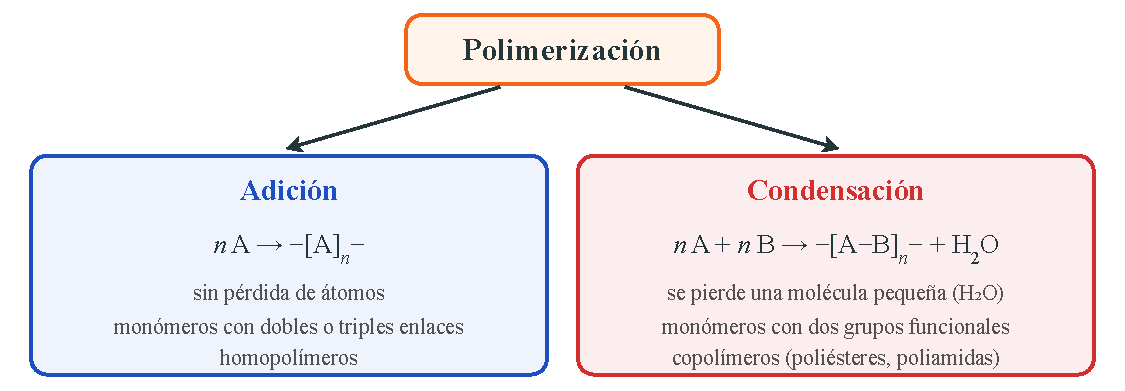
\includegraphics[width=0.85\linewidth]{FigurasSVG/UD10_Polimeros/pdf/UD10_01_tipos_polimerizacion.pdf}
        \caption{Tipos de polimerización}
        \label{fig:tipos-polimerizacion}
    \end{figure}


    \section{Polímeros de adición}

    La masa molecular del polímero es
    un múltiplo exacto de la masa molecular del monómero, pues al formarse la
    cadena los monómeros se unen sin perder ningún átomo. Los monómeros tienen
    insaturaciones (dobles o triples enlaces) que pasan a sencillos en el polímero.


    Suelen seguir un mecanismo en tres fases, con
    ruptura homolítica del enlace:

    \begin{itemize}
        \item \textbf{Iniciación}.% \marcador{poner esquema}
            \begin{figure}[H]
                \centering
                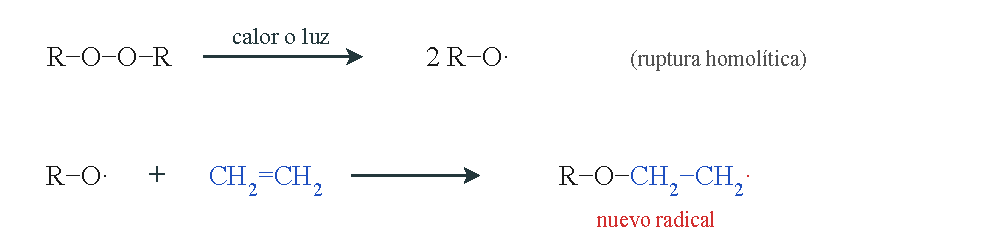
\includegraphics[width=0.8\linewidth]{FigurasSVG/UD10_Polimeros/pdf/UD10_02_iniciacion.pdf}
                \caption{Iniciación de la polimerización por adición}
                \label{fig:polimerizacion-iniciacion}
            \end{figure}
        \item \textbf{Propagación o crecimiento}. % \marcador{poner esquema}
            \begin{figure}[H]
                \centering
                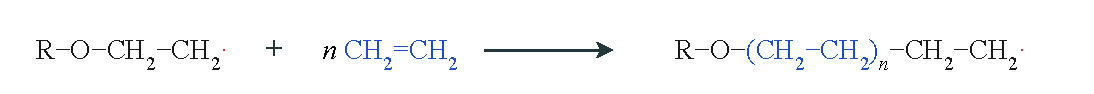
\includegraphics[width=0.9\linewidth]{FigurasSVG/UD10_Polimeros/pdf/UD10_03_propagacion.pdf}
                \caption{Propagación de la cadena}
                \label{fig:polimerizacion-propagacion}
            \end{figure}
        \item \textbf{Terminación}. Los radicales libres de los extremos se unen a impurezas o bien se unen dos cadenas con un terminal neutralizado.
            \begin{figure}[H]
                \centering
                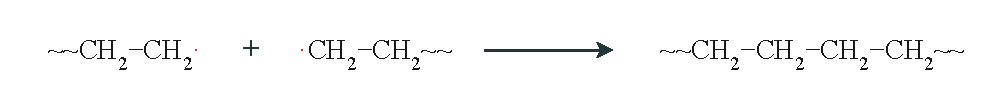
\includegraphics[width=0.8\linewidth]{FigurasSVG/UD10_Polimeros/pdf/UD10_04_terminacion.pdf}
                \caption{Terminación por combinación de dos radicales}
                \label{fig:polimerizacion-terminacion}
            \end{figure}
    \end{itemize}

    Veamos algunos de los polímeros de
    adición más importantes, sus principales aplicaciones, así como los monómeros
    de los que proceden. Nótese que los polímeros de adición son homopolímeros y basan
    su nomenclatura en el nombre comercial de los monómeros.

    \begin{figure}[H]
        \centering
        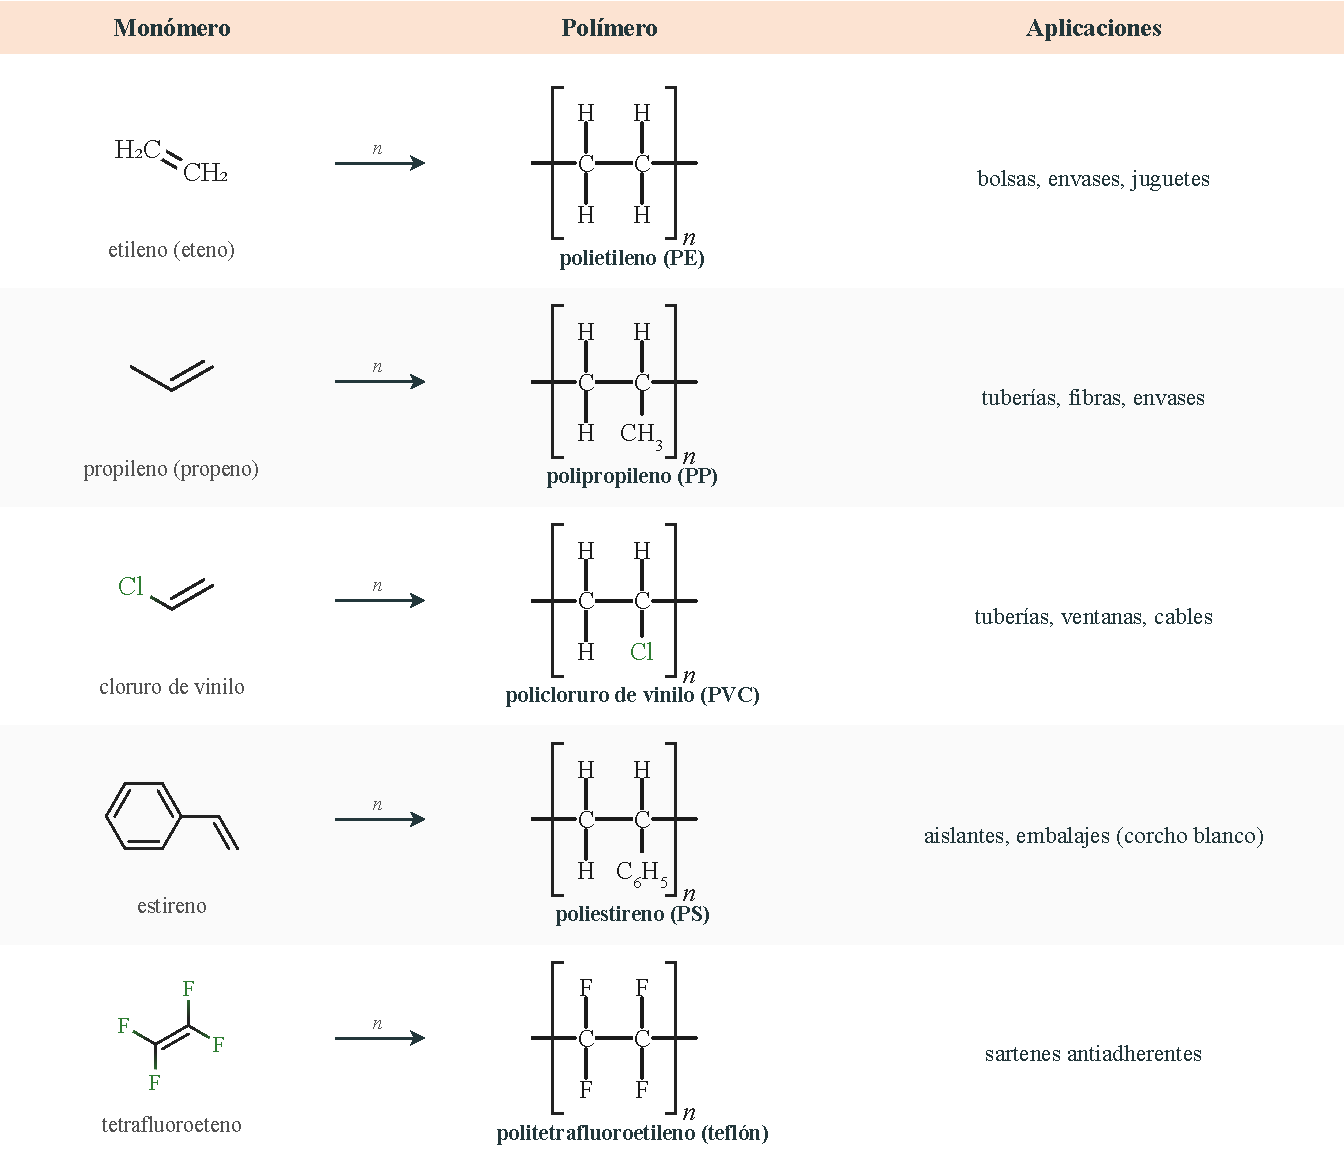
\includegraphics[width=1.0\linewidth]{FigurasSVG/UD10_Polimeros/pdf/UD10_05_polimeros_adicion.pdf}
        \caption{Principales polímeros de adición}
        \label{fig:polimeros-adicion}
    \end{figure}


    \section{Polímeros de condensación}

    Se produce por la unión de monómeros con pérdida de una molécula pequeña, por ejemplo agua. Por tanto, la masa molecular del polímero no es un múltiplo exacto de la masa molecular del monómero. Los polímeros son mucho más pequeños que los de adición y son heteropolímeros (copolímeros), ya que los monómeros de partida tienen que ser distintos.

	Los principales polímeros de condensación son:

    \begin{enumerate}[label=\numberballmDarkTeal]
        \item \negsubro{Poliésteres}. Los poliésteres son unos polímeros que contiene el grupo funcional éster en su cadena principal que se repite \( n \) veces.

        Se producen por sucesivas reacciones de esterificación (alcohol y ácido). Para formar la función éster a los dos lados de la cadena se requiere que uno de los monómeros sea un diácido y el otro un diol terminal.

        El poliéster más conocido es el formado por ácido tereftálico (ácido p-benceno-dicarboxilico) y el etilenglicol (etanodiol) que se puede obtener como fibra textil llamada tergal (dacrón) o como plástico que se conoce como PET:

        \begin{figure}[H]
            \centering
            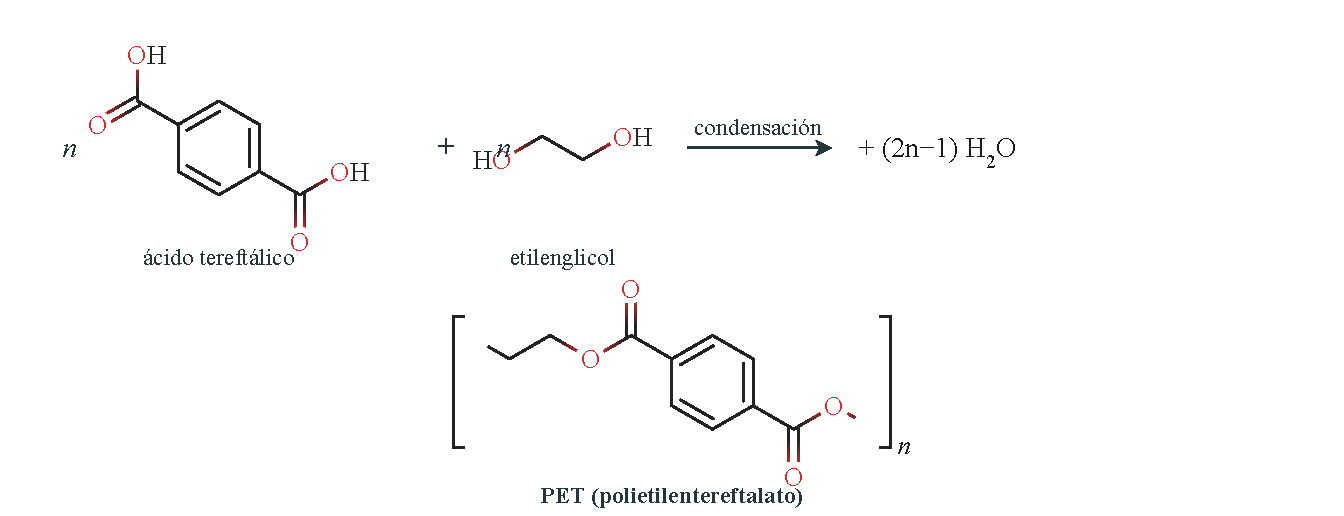
\includegraphics[width=0.95\linewidth]{FigurasSVG/UD10_Polimeros/pdf/UD10_06_formacion_PET.pdf}
            \caption{Formación del PET}
            \label{fig:formacion-pet}
        \end{figure}

        \textbf{Aplicaciones:}  fibra textil , envases de licores, medicamentos y alimentos, reparación de vasos sanguíneos…
        \item \negsubro{Poliamidas}. Son unos polímeros que contiene el grupo funcional amida en su cadena principal que se repite n veces.

        Se producen por sucesivas reacciones entre el grupo ácido y el amino. Para formar la función amida a los dos lados de la cadena se requiere que uno de los monómeros sea un diácido y el otro una diamina:

        La poliamida más conocida es el nailon 6,6  (conocido como seda artificial) formado por la copolimerización del ácido adípico  (ácido hexanodioico) y la 1,6-hexanodiamina:

        \begin{figure}[H]
            \centering
            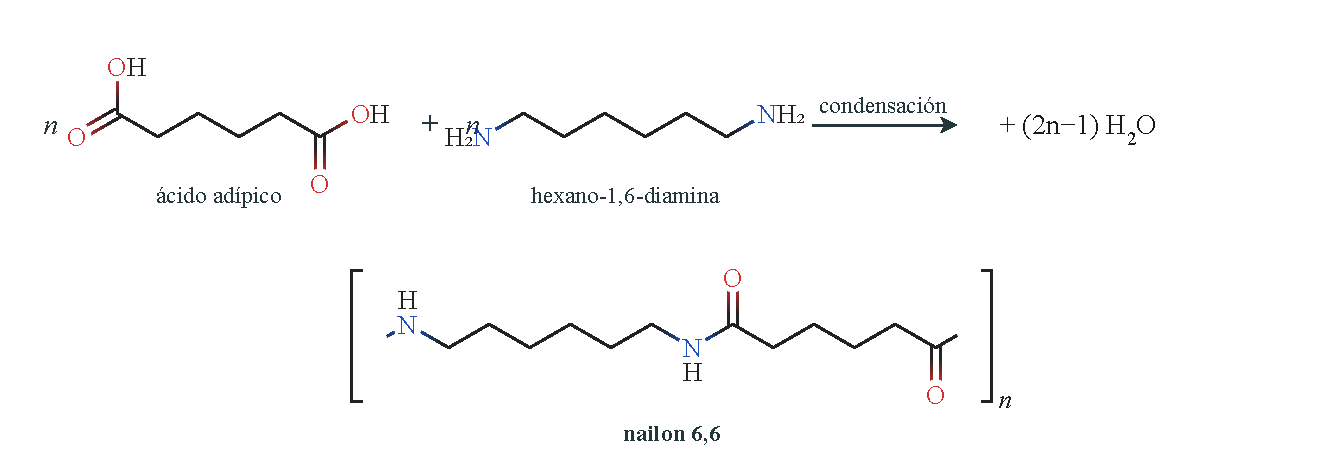
\includegraphics[width=0.95\linewidth]{FigurasSVG/UD10_Polimeros/pdf/UD10_07_formacion_nailon_66.pdf}
            \caption{Formación del nailon 6,6}
            \label{fig:formacion-nailon}
        \end{figure}

        Aplicaciones: Forma fibras muy resistentes por lo que se pueden utilizar para telas de paracaídas, sedales, medias, cepillos, cerdas, peines…


    \end{enumerate}








%----------------------------------------------------------------------------------------
%	TABLE OF CONTENTS

%----------------------------------------------------------------------------------------

    \pagestyle{empty} % Disable headers and footers for the following pages

    %\tableofcontents % Output the table of contents

    %\listoffigures % Output the list of figures, comment or remove this command if not required

    %\listoftables % Output the list of tables, comment or remove this command if not required

    %\pagestyle{fancy} % Enable default headers and footers again

    %\cleardoublepage % Start the following content on a new page


%----------------------------------------------------------------------------------------
%	SOLUTIONS
%----------------------------------------------------------------------------------------


    \part{Soluciones a los ejercicios}



%----------------------------------------------------------------------------------------
%	SECTIONING EXAMPLES CHAPTER
%----------------------------------------------------------------------------------------

    \chapterimage{orange3.jpg} % Chapter heading image
    \chapterspaceabove{6.75cm} % Whitespace from the top of the page to the chapter title on chapter pages
    \chapterspacebelow{7.25cm} % Amount of vertical whitespace from the top margin to the start of the text on chapter pages

%-----------------------------------------------

    \chapter{Soluciones}

    \pagestyle{fancy}

    \Closesolutionfile{ans}


    \input{soluciones}


%----------------------------------------------------------------------------------------
%	PART
%----------------------------------------------------------------------------------------



\end{document}
